\documentclass[12pt]{article}
\usepackage[utf8]{inputenc}
\usepackage{graphicx}
\usepackage{float}
\usepackage{booktabs,bigstrut}
\usepackage{multirow,multicol}
\usepackage{natbib}
\usepackage{amsmath,amssymb,amsfonts,latexsym,cancel}
\usepackage{tikz}
\usetikzlibrary{positioning}
\usepackage{pgfplots,caption}
\usepackage{comment}
\usepackage{pdflscape}
\usepackage{colortbl}
\usepackage{longtable}
\usepackage{xcolor}
\usepackage{rotating}
\usepackage{cancel}
\usepackage{parskip}
\usepackage{multicol}
\usepackage{hhline}
\usepackage{array}
\usepackage{longtable,lscape}
\usepackage[most]{tcolorbox}%Para colorear respuestas de ecuaciones
%\tcbset{enhanced,colframe=blue,colback={black!5!white},drop shadow}
%\tcboxmath[colframe=blue]{\mathbf{0.41\%}}


%All the packages the project needs
%--------------------------------------------
%Margins
\usepackage[top=1.5cm,
bottom=1.5cm,
left=2.5cm,
right=2cm,
headsep=15pt,
headheight=25pt,
letterpaper,
includehead,includefoot]{geometry} 
%-------------------------------------------

%-------------------------------------------
%Codification and language
%Document language
\usepackage[spanish,es-noshorthands]{babel}
% Required for including letters with accents
\usepackage[utf8]{inputenc} 
% Use 8-bit encoding that has 256 glyphs
\usepackage[T1]{fontenc}
%-------------------------------------------

%-------------------------------------------
%Colours
\usepackage{color}
\usepackage{xcolor}
%-------------------------------------------

%-------------------------------------------
%Fonts and text
%Add a new Font
\usepackage{addfont}
\addfont{OT1}{rsfs10}{\rsfs}
%Allows to modify the font of a section
\usepackage{sectsty}
%Latin Modern fonts - Allows to resize the font
\usepackage{lmodern}
%Allows to write code
\usepackage{verbatim}
%Dumb text
\usepackage{lipsum}
%Include currency symbols
\usepackage{textcomp} 
%-------------------------------------------

%-------------------------------------------
%Pictures and graphics
%Allows to include images
\usepackage{graphicx}
\usepackage{sidecap}
%Most powerful image package
\usepackage{tikz}
\usetikzlibrary{babel}
\usetikzlibrary{positioning}
%Sometimes used images packages

\usepackage{pst-all}
\usepackage{pstricks}
%Allows to position figures inside a paragraph
\usepackage{wrapfig}
%Information needed
%https://en.wikibooks.org/wiki/LaTeX/Floats,_Figures_and_Captions
%-------------------------------------------
%-------------------------------------------
%Math packages
\usepackage{mathtools}
%\usepackage{unicode-math}
\usepackage{amsmath}
\usepackage{amssymb}
\usepackage{amsfonts}
%Nice cancelations arrows
\usepackage{cancel}
%Vector arrows on a character
\usepackage{esvect}
%-------------------------------------------

%-------------------------------------------
%Table and listing packages
\usepackage{multirow}
\usepackage{array}
\usepackage{diagbox}
\usepackage{listings}
\usepackage[shortlabels]{enumitem} 
%Differents images and tables in the same space
\usepackage{subcaption}
%Use to places the float at precisely the location in the LaTeX code´and other stuff
\usepackage{float}
%Flexible tables
\usepackage{tabu}
\usepackage{multicol}
%-------------------------------------------

%-------------------------------------------
%Refs and cites
%\usepackage{achemso}
%\usepackage{natbib}
\usepackage{hyperref}
\hypersetup{
colorlinks=true,
urlcolor= blue,
citecolor=blue,
linkcolor= black,
bookmarks=true,
bookmarksopen=true,
}
\usepackage{csquotes}
\usepackage[backend=biber]{biblatex}
%\usepackage{cite}
%-------------------------------------------

%-------------------------------------------
%Boxes
\usepackage{tcolorbox}
\usepackage{fancybox}
\usepackage{colortbl}
%-------------------------------------------

%-------------------------------------------
%Page style
\usepackage[usestackEOL]{stackengine}
\usepackage{fancyhdr}
\pagestyle{fancy}
\newsavebox{\UNl}
\newsavebox{\UNd}
\setlength{\headheight}{2.5cm}
\lhead{\usebox{\UNl}\usebox{\UNd}}
\rhead{\slshape Proyecto de Tesis}
\cfoot{}
\rfoot{\thepage}
%\lfoot{\today}
\renewcommand{\headrulewidth}{1pt}

%-------------------------------------------

%-------------------------------------------
%others
\usepackage{pgfplots,caption}
\usepackage{comment}
\usepackage{pdflscape}
\usepackage{rotating}
\usepackage{parskip}
\usepackage{hhline}
\usepackage{longtable,lscape}
\usepackage{booktabs,bigstrut}
\usepackage{enumerate}
\usepackage{cleveref}
\usepackage{braket}

\title{TALLER1}
\author{Juan David Torres}
\date{\today}
%Inicio del documento
\pgfplotsset{compat=1.17}
\begin{document}
\renewcommand{\tablename}{Tabla}%% Para cambiar "Cuadro" a "Tabla"
\renewcommand{\listtablename}{Índice de tablas}
%Inicio de la portada
\begin{titlepage}
    \thispagestyle{empty}
    \begin{center}
        \begin{figure}
        \centering%
        
\includegraphics{images/EscudoUN.png}
    \end{figure}
    
    \vspace{1cm}
    
        \textbf{PROYECTO DISEÑO ESTRUCTURAL\\MEMORIAS DE CÁLCULO}\\[1.3in]
      
    JUAN MANUEL CÓRDOBA PEÑA \\  
    JUAN DAVID TORRES TURRIAGO \\
    EDUARDO ANDRÉS DELGADILLO MONSALVE \\  [1.5in]
 Trabajo presentado como requisito parcial de la asignatura\\  DISEÑO ESTRUCTURAL  al docente:\\[3mm] \textbf {\large{Ing. Ismael Santana Santana}}\\[1.5in]
   \textbf{UNIVERSIDAD NACIONAL DE COLOMBIA}\\
   FACULTAD DE INGENIERÍA CIVIL Y AGRÍCOLA\\
   BOGOTÁ D.C.\\
   \today
    \end{center}
\end{titlepage}

\newpage
\thispagestyle{empty}
\tableofcontents
\thispagestyle{empty}
\newpage

% \listoffigures

% \listoftables

\newpage

\setcounter{page}{1}
\section{Descripción del proyecto}

El proyecto se encuentra ubicado en la ciudad de Bogotá D.C en la microzonificación sísmica de "Lacustre 100". Consiste en una edificación  de cuatro pisos con una altura libre entre losas de 2.5 metros, que tiene un sistema estructural de pórtico de concreto reforzado resistente a momentos con capacidad moderada de disipación de energía (DMO) y cuyo tipo de uso es vivienda. La losa de entrepiso y de cubierta es aligerada y armada en una dirección.\\

Para encontrar el espesor mínimo de la losa se utilizaron las alturas promedio dadas por las tablas C.R.9.5 y C.9.5(a) de la NSR-10, para no incurrir en un costo alto de losa, obteniéndose un valor de $\mathbf{h_{losa}=0.5m}$. De acuerdo a C.8.13.2 se determina un ancho de viguetas de \textbf{0.10 m} y a partir de C.8.13.3 se encuentra una separación entre viguetas que no supere 1.2 m. Se colocan riostras transversales a las viguetas de manera tal que su separación no exceda 4.0 m de acuerdo con C.8.13.3.1. A partir de C.8.13.6, se determina un espesor de plaqueta superior de \textbf{0.05 m} que se vaciara en un casetón removible.\\


\section{Definición de la carga viva}

Para el cálculo de la carga viva en la estructura se utiliza el valor indicado en la norma NSR-10, específicamente en la \textit{tabla B.4.2.1.1-Cargas vivas  uniformemente distribuidas}, con el cual se obtiene que el valor de la carga viva corresponde a $ \mathbf{1.8 \tfrac{kN}{m^{2}}}$ para el uso de la edificación (residencial). Adicionalmente, de acuerdo con la norma, se establece una carga de $ \mathbf{3.0 \tfrac{kN}{m^{2}}}$ para la escalera. Con respecto a la cubierta se toma una carga viva mínima de $ \mathbf{1.8 \tfrac{kN}{m^{2}}}$ de acuerdo con la tabla B.4.2.1-2. Para el ascensor se considera una carga viva de $ \mathbf{20 \tfrac{kN}{m^{2}}}$  en donde se tiene en cuenta la carga de impacto.\\ 

\section{Evaluación de las cargas muertas}

La evaluación de la carga muerta se realiza teniendo en cuenta que el material que se utilizará para construir la estructura es el concreto armado, cuyo peso por unidad de volumen corresponde a 24 $\frac{kN}{m^{2}}$ de acuerdo con la tabla B.3.2-1 de la NSR-10.\\

\subsection{Evaluación carga muerta piso tipo}

Teniendo en cuenta que el material de la estructura consiste en concreto armado, se calcula la carga muerta del piso tipo por cada  elementos que compone a la losa aligerada en una dirección: la plaqueta, viguetas, riostras y el casetón. Esto se realiza teniendo en cuenta el peso de los muros divisorios, los acabados y las instalaciones que reposan sobre cada piso, pues con este se realiza el aligeramiento. A continuación, se presenta una tabla resumen de cada elemento y el peso por metro cuadrado con su correspondiente operación.



% Table generated by Excel2LaTeX from sheet 'Eval. Cargas'
\begin{table}[H]
  \centering
  
    \begin{tabular}{cc|r|c|}
    \rowcolor[rgb]{ .2,  .247,  .31} \multicolumn{4}{|c}{\textcolor[rgb]{ 1,  1,  1}{\textbf{CARGAS MUERTAS}}} \bigstrut[b]\\
    \hline
    \rowcolor[rgb]{ .2,  .247,  .31} \multicolumn{2}{|c|}{\textcolor[rgb]{ 1,  1,  1}{Elemento}} & \multicolumn{1}{c|}{\textcolor[rgb]{ 1,  1,  1}{Operación }} & \textcolor[rgb]{ 1,  1,  1}{Resultado} \bigstrut[b]\\
    \hline
    \rowcolor[rgb]{ .2,  .247,  .31} \multicolumn{2}{|c|}{\textcolor[rgb]{ 1,  1,  1}{Plaqueta [kN/m²]}} & \multicolumn{1}{c|}{\cellcolor[rgb]{ 1,  1,  1}0.05 $m\cdot $ 24$\frac{kN}{m^{3}}$} & \cellcolor[rgb]{ 1,  1,  1}1.2 \bigstrut\\
    \hline
    \rowcolor[rgb]{ .2,  .247,  .31} \multicolumn{2}{|c|}{\textcolor[rgb]{ 1,  1,  1}{Viguetas [kN/m²]}} & \multicolumn{1}{c|}{\cellcolor[rgb]{ 1,  1,  1}$\dfrac{0.1\;m\cdot0.45\;m\cdot 24\frac{kN}{m^{3}}}{ 0.87\; m}$} & \cellcolor[rgb]{ 1,  1,  1}1.24 \bigstrut\\
    \hline
    \rowcolor[rgb]{ .2,  .247,  .31} \multicolumn{2}{|c|}{\textcolor[rgb]{ 1,  1,  1}{Riostras [kN/m²]}} & \multicolumn{1}{c|}{\cellcolor[rgb]{ 1,  1,  1}$\dfrac{0.1\;m\cdot0.45\;m\cdot 24\frac{kN}{m^{3}}}{6.95\;m}$} & \cellcolor[rgb]{ 1,  1,  1}0.16 \bigstrut\\
    \hline
    \rowcolor[rgb]{ .2,  .247,  .31} \multicolumn{2}{|c|}{\textcolor[rgb]{ 1,  1,  1}{Casetón[kN/m²]}} & \multicolumn{1}{c|}{\cellcolor[rgb]{ 1,  1,  1}0.35} & \cellcolor[rgb]{ 1,  1,  1}0.35 \bigstrut\\
    \hline
    \rowcolor[rgb]{ .2,  .247,  .31} \multicolumn{2}{|c|}{\textcolor[rgb]{ 1,  1,  1}{Muros (residencial)[kN/m²]}} & \multicolumn{1}{c|}{\cellcolor[rgb]{ 1,  1,  1}3} & \cellcolor[rgb]{ 1,  1,  1}3 \bigstrut\\
    \hline
    \rowcolor[rgb]{ .2,  .247,  .31} \multicolumn{2}{|c|}{\textcolor[rgb]{ 1,  1,  1}{Acabado superior}} & \multicolumn{1}{c|}{\cellcolor[rgb]{ 1,  1,  1}$0.05\;m \cdot 21 \dfrac{kN}{m^3}$} & \cellcolor[rgb]{ 1,  1,  1}1.05 \bigstrut\\
    \hline
    \rowcolor[rgb]{ .2,  .247,  .31} \multicolumn{2}{|c|}{\textcolor[rgb]{ 1,  1,  1}{Acabado inferior}} & \multicolumn{1}{c|}{\cellcolor[rgb]{ 1,  1,  1}0.3} & \cellcolor[rgb]{ 1,  1,  1}0.3 \bigstrut\\
    \hline
    \rowcolor[rgb]{ .2,  .247,  .31} \multicolumn{2}{|c|}{\textcolor[rgb]{ 1,  1,  1}{Instalaciones}} & \multicolumn{1}{c|}{\cellcolor[rgb]{ 1,  1,  1}0.2} & \cellcolor[rgb]{ 1,  1,  1}0.2 \bigstrut\\
    \hline
    \rowcolor[rgb]{ .2,  .247,  .31} \multicolumn{2}{c|}{\textcolor[rgb]{ 1,  1,  1}{\textbf{TOTAL}}} & \cellcolor[rgb]{ 1,  1,  1} & \cellcolor[rgb]{ 1,  1,  1}7.50 \bigstrut\\
\cline{3-4}    \end{tabular}%
    \caption{Evaluación cargas muertas piso tipo}
  \label{tab:CMPT}%
\end{table}%




Sumando estos elementos tenemos los siguientes resultados por el piso tipo resumidos en la siguiente tabla, calculando la carga última como el resultado mayor entre $1.2D+1.6L$ y $1.4D$, el factor de carga como la división de la carga última entre la carga total.

% Table generated by Excel2LaTeX from sheet 'Eval. Cargas'
\begin{table}[H]
  \centering
  
    \begin{tabular}{|c|c|c|c|}
    \hline
    \rowcolor[rgb]{ .2,  .247,  .31} \multicolumn{2}{|c|}{\textcolor[rgb]{ 1,  1,  1}{\textbf{CARGA MUERTA (D) [kN/m²]}}} & \cellcolor[rgb]{ 1,  1,  1} ver tabla \ref{tab:CMPT} & \cellcolor[rgb]{ 1,  1,  1}7.5 \bigstrut\\
    \hline
    \rowcolor[rgb]{ .2,  .247,  .31} \multicolumn{2}{|c|}{\textcolor[rgb]{ 1,  1,  1}{\textbf{CARGA VIVA (L) [kN/m²]}}} & \cellcolor[rgb]{ 1,  1,  1}(tomado de la norma) & \cellcolor[rgb]{ 1,  1,  1}1.8 \bigstrut\\
    \hline
    \rowcolor[rgb]{ .2,  .247,  .31} \multicolumn{2}{|c|}{\textcolor[rgb]{ 1,  1,  1}{\textbf{CARGA TOTAL [kN/m²]}}} & \cellcolor[rgb]{ 1,  1,  1}$7.5 \tfrac{kN}{m^2} + 1.8  \tfrac{kN}{m^2}$  & \cellcolor[rgb]{ 1,  1,  1}9.30\bigstrut\\
    \hline
    \rowcolor[rgb]{ .2,  .247,  .31} \multicolumn{2}{|c|}{\textcolor[rgb]{ 1,  1,  1}{\textbf{CARGA ÚLTIMA [kN/m²]}}} & \cellcolor[rgb]{ 1,  1,  1}$1.2 \cdot7.5 \tfrac{kN}{m^2} + 1.6 \cdot 1.8  \tfrac{kN}{m^2}$ & \cellcolor[rgb]{ 1,  1,  1}11.88 \bigstrut\\
    \hline
    \rowcolor[rgb]{ .2,  .247,  .31} \multicolumn{2}{|c|}{\textcolor[rgb]{ 1,  1,  1}{\textbf{FACTOR DE CARGA}}} & \cellcolor[rgb]{ 1,  1,  1}$\dfrac{11.88}{9.30}$ & \cellcolor[rgb]{ 1,  1,  1}1.28 \bigstrut\\
    \hline
    \end{tabular}%
    \caption{Resultados de la carga del piso tipo}
  \label{tab:Resultados de la carga del piso tipo}%
\end{table}%



\subsection{Evaluación carga muerta de cubierta}

De manera análoga a la evaluación de carga muerta del piso tipo se realiza la evaluación de cargas de la cubierta, teniendo en cuenta los elementos que componen la losa aligerada en una dirección: la plaqueta, las viguetas, riostras y el casetón. Adicionalmente en este caso se aplicará un impermeabilizante, para evitar la exposición a la intemperie de los elementos internos de la edificación.   El material escogido es la tela asfáltica, que tiene un valor de $0.03\: kN/m^2$ de acuerdo a la tabla B.3.4.1-4.\\

Se realiza un análisis de los muros perimetrales de la edificación teniendo en cuenta la geometría de la misma. El peso de los muros corresponde al producto entre el peso que aportan los muros exteriores y la razón entre al área vertical y el área de la losa. Se toman muros exteriores con enchape en ladrillo tomando el valor de la tabla B.3.4.2-4, el cual corresponde a un valor de $2.5 kN/m^2$ por área vertical y para los muros internos se tomó mampostería pañetada de espesor de 15 cm que tiene el mismo peso de los muros perimetrales de acuerdo a la norma NSR-10. A continuación, se presenta una tabla resumen de cada elemento y el peso por metro cuadrado con su correspondiente operación.

% Table generated by Excel2LaTeX from sheet 'Eval. Cargas'
\begin{table}[H]
  \centering
 
    \begin{tabular}{cc|r|c|}
    \rowcolor[rgb]{ .2,  .247,  .31} \multicolumn{4}{|c}{\textcolor[rgb]{ 1,  1,  1}{\textbf{CARGAS MUERTAS}}} \bigstrut[b]\\
    \hline
    \rowcolor[rgb]{ .2,  .247,  .31} \multicolumn{2}{|c|}{\textcolor[rgb]{ 1,  1,  1}{Elemento}} & \multicolumn{1}{c|}{\textcolor[rgb]{ 1,  1,  1}{Operación }} & \textcolor[rgb]{ 1,  1,  1}{Resultado} \bigstrut[b]\\
    \hline
    \rowcolor[rgb]{ .2,  .247,  .31} \multicolumn{2}{|c|}{\textcolor[rgb]{ 1,  1,  1}{Plaqueta [kN/m²]}} & \multicolumn{1}{c|}{\cellcolor[rgb]{ 1,  1,  1}0.05 $m\cdot $ 24$\frac{kN}{m^{3}}$} & \cellcolor[rgb]{ 1,  1,  1}1.2 \bigstrut\\
    \hline
    \rowcolor[rgb]{ .2,  .247,  .31} \multicolumn{2}{|c|}{\textcolor[rgb]{ 1,  1,  1}{Viguetas [kN/m²]}} & \multicolumn{1}{c|}{\cellcolor[rgb]{ 1,  1,  1}$\dfrac{0.1\;m\cdot0.45\;m\cdot 24\frac{kN}{m^{3}}}{ 0.87\; m}$} & \cellcolor[rgb]{ 1,  1,  1}1.24 \bigstrut\\
    \hline
    \rowcolor[rgb]{ .2,  .247,  .31} \multicolumn{2}{|c|}{\textcolor[rgb]{ 1,  1,  1}{Riostras [kN/m²]}} & \multicolumn{1}{c|}{\cellcolor[rgb]{ 1,  1,  1}$\dfrac{0.1\;m\cdot0.45\;m\cdot 24\frac{kN}{m^{3}}}{6.95\;m}$} & \cellcolor[rgb]{ 1,  1,  1}0.16\bigstrut\\
    \hline
    \rowcolor[rgb]{ .2,  .247,  .31} \multicolumn{2}{|c|}{\textcolor[rgb]{ 1,  1,  1}{Casetón[kN/m²]}} & \multicolumn{1}{c|}{\cellcolor[rgb]{ 1,  1,  1}0.35} & \cellcolor[rgb]{ 1,  1,  1}0.35 \bigstrut\\
    \hline
    \rowcolor[rgb]{ .2,  .247,  .31} \multicolumn{2}{|c|}{\textcolor[rgb]{ 1,  1,  1}{Muros (perimetrales y de vacíos) [kN/m²]}} & \multicolumn{1}{c|}{\cellcolor[rgb]{ 1,  1,  1}$2.5\tfrac{kN}{m^2} \cdot\frac{(82.2\;m + 6.54\;m)\cdot 1.5\;m}{397.48\; m^2}$} & \cellcolor[rgb]{ 1,  1,  1}0.84 \bigstrut\\
    \hline
    \rowcolor[rgb]{ .2,  .247,  .31} \multicolumn{2}{|c|}{\textcolor[rgb]{ 1,  1,  1}{Pendientado}} & \multicolumn{1}{c|}{\cellcolor[rgb]{ 1,  1,  1}$0.05\;m \cdot 21 \dfrac{kN}{m^3}$} & \cellcolor[rgb]{ 1,  1,  1}1.05 \bigstrut\\
    \hline
    \rowcolor[rgb]{ .2,  .247,  .31} \multicolumn{2}{|c|}{\textcolor[rgb]{ 1,  1,  1}{Acabados inferior}} & \multicolumn{1}{c|}{\cellcolor[rgb]{ 1,  1,  1}0.3} & \cellcolor[rgb]{ 1,  1,  1}0.3 \bigstrut\\
    \hline
    \rowcolor[rgb]{ .2,  .247,  .31} \multicolumn{2}{|c|}{\textcolor[rgb]{ 1,  1,  1}{Acabados (impermeabilización)}} & \multicolumn{1}{c|}{\cellcolor[rgb]{ 1,  1,  1}0.03} & \cellcolor[rgb]{ 1,  1,  1}0.03 \bigstrut\\
    \hline
    \rowcolor[rgb]{ .2,  .247,  .31} \multicolumn{2}{|c|}{\textcolor[rgb]{ 1,  1,  1}{Instalaciones}} & \multicolumn{1}{c|}{\cellcolor[rgb]{ 1,  1,  1}0.2} & \cellcolor[rgb]{ 1,  1,  1}0.2 \bigstrut\\
    \hline
    \rowcolor[rgb]{ .2,  .247,  .31} \multicolumn{2}{c|}{\textcolor[rgb]{ 1,  1,  1}{\textbf{TOTAL}}} & \cellcolor[rgb]{ 1,  1,  1} & \cellcolor[rgb]{ 1,  1,  1}5.37 \bigstrut\\
\cline{3-4}    \end{tabular}%
 \caption{Evaluación de cargas muertas de cubierta}
  \label{tab:EvaDC}%
\end{table}%





De igual manera, se suman todos los elementos, se encuentra el valor de la carga última y el factor de carga.



% Table generated by Excel2LaTeX from sheet 'Eval. Cargas'
\begin{table}[H]
  \centering

    \begin{tabular}{|c|c|c|c|}
    
    \rowcolor[rgb]{ .2,  .247,  .31} \multicolumn{2}{|c|}{\textcolor[rgb]{ 1,  1,  1}{Elemento}} & \multicolumn{1}{c|}{\textcolor[rgb]{ 1,  1,  1}{Operación }} & \textcolor[rgb]{ 1,  1,  1}{Resultado} \bigstrut[b]\\
    \hline
    \rowcolor[rgb]{ .2,  .247,  .31} \multicolumn{2}{|c|}{\textcolor[rgb]{ 1,  1,  1}{\textbf{CARGA MUERTA (D) [kN/m²]}}} & \cellcolor[rgb]{ 1,  1,  1} Ver tabla \ref{tab:EvaDC} & \cellcolor[rgb]{ 1,  1,  1}5.37 \bigstrut\\
    \hline
    \rowcolor[rgb]{ .2,  .247,  .31} \multicolumn{2}{|c|}{\textcolor[rgb]{ 1,  1,  1}{\textbf{CARGA VIVA (L) [kN/m²]}}} & \cellcolor[rgb]{ 1,  1,  1} Tomado de la norma & \cellcolor[rgb]{ 1,  1,  1}1.8 \bigstrut\\
    \hline
    \rowcolor[rgb]{ .2,  .247,  .31} \multicolumn{2}{|c|}{\textcolor[rgb]{ 1,  1,  1}{\textbf{CARGA TOTAL [kN/m²]}}} & \cellcolor[rgb]{ 1,  1,  1}5.37 $\tfrac{kN}{m^2}$+1.8 $\frac{kN}{m^2}$ & \cellcolor[rgb]{ 1,  1,  1}7.17 \bigstrut\\
    \hline
    \rowcolor[rgb]{ .2,  .247,  .31} \multicolumn{2}{|c|}{\textcolor[rgb]{ 1,  1,  1}{\textbf{CARGA ÚLTIMA [kN/m²]}}} & \cellcolor[rgb]{ 1,  1,  1}$1.2\cdot5.37$ $\tfrac{kN}{m^2}$+$1.6\cdot1.8$ $\tfrac{kN}{m^2}$ & \cellcolor[rgb]{ 1,  1,  1}9.32 \bigstrut\\
    \hline
    \rowcolor[rgb]{ .2,  .247,  .31} \multicolumn{2}{|c|}{\textcolor[rgb]{ 1,  1,  1}{\textbf{FACTOR DE CARGA}}} & \cellcolor[rgb]{ 1,  1,  1}$\dfrac{9.32}{7.17}$ & \cellcolor[rgb]{ 1,  1,  1}1.30 \bigstrut\\
    \hline
    \end{tabular}%
      \caption{Resultados de la carga de cubierta}
  \label{tab:RDR}%
\end{table}%


\subsection{Evaluación de cargas de la escalera}


Partiendo de un ancho de huella de $0.28\;m$ se determina la altura de la contrahuella teniendo en cuenta los requisitos de K.3.8.3.4. Se establecen 18 escalones con una altura de contrahuella de $170\;mm$. La longitud del tramo inclinado es de $2.24\;m$ y la longitud del descanso de $1.2\;m$\\


Teniendo en cuenta las consideraciones del inciso C.9.5, el espesor de la losa de la escalera se calcula teniendo en cuenta que esta es simplemente apoyada, por lo que se toma un espesor de: $l/20$
\begin{equation}
    t=\frac{l}{20}=\frac{3.44\;m}{20}=0.172\;m \Rightarrow 0.15\;m
\end{equation}
Este valor se reduce a $0.15\;m$ \\ %justificar
Para encontrar la pendiente de la losa se toma la suma de las huellas ($2.24\;m$) y la altura de la contrahuella sin tomar la última ($1.33\;m$)

\begin{equation}
    \theta=tan^{-1}\left(\frac{1.33}{2.24}\right)=30.70^{\circ}
\end{equation}


\begin{table}[H]
\centering

\begin{tabular}{|c|c|c|} 
\hline
\multicolumn{3}{|c|}{{\cellcolor[rgb]{0.227,0.227,0.227}}\textcolor{white}{\textbf{EVALUACIÓN CARGAS TRAMO INCLINADO}}}                                 \\ 
\hline
\rowcolor[rgb]{0.227,0.227,0.227} \textcolor{white}{\textbf{Elemento}} & \textcolor{white}{\textbf{Operación}} & \textcolor{white}{\textbf{Resultado}}  \\ 
\hline
{\cellcolor[rgb]{1 ,1 ,1}}Peso propio losa
  kN/m²           &   $\frac{0.15\;m \cdot 24 \tfrac{KN}{m^3}}{\cos{30.70^{\circ}}}$                                  & 4.19                                 \\ 
\hline
{\cellcolor[rgb]{1,1,1}}Peso de peldaños
  kN/m²           & $\frac{0.17\;m \cdot 24 \tfrac{KN}{m^3}}{2}$                                     & 2.04                                 \\ 
\hline  
{\cellcolor[rgb]{1,1,1}}Acabado (baldosa 25
  mm) kN/m²    &  $\frac{0.28\;m + 0.17\;m}{0.28\;m}\cdot 1.1\tfrac{KN}{m^2}$                                    & 1.77                                   \\ 
\hline
{\cellcolor[rgb]{1,1,1}}Cielo raso falso kN/m²                   & $\frac{0.3}{\cos{30.70^{\circ}}}$                                      & 0.35                                   \\ 
\hline
{\cellcolor[rgb]{1,1,1}}Subtotal (Carga
  muerta~ kN/m²)   & $\mathbf{\sum}$                                    & \textbf{8.34  }                                 \\ 
\hline
{\cellcolor[rgb]{1,1,1}}Carga viva kN/m²                   & (Tomado de la norma)                                     & \textbf{3.00}                                   \\ 
\hline
{\cellcolor[rgb]{1,1,1}}\textbf{TOTAL}                     & ~                                     & \textbf{11.34}                         \\
\hline
\end{tabular}
\caption{Evaluación de cargas del tramo inclinado de la escalera}
\label{tab:evalINCLIN}
\end{table}

Con las dimensiones de contrahuella, huella y pendiente se analizan las cargas en $kN/m^2$ para el tramo inclinado,dando como resultado una carga muerta de: $\mathbf{8.34\; \tfrac{kN}{m^2}}$.\\

De acuerdo con la tabla B.4.2.1-1 de la NSR-10 se toma una carga viva para la la escalera de  $\mathbf{3.0 \tfrac{KN}{m^2}}$ \\

El procedimiento mostrado en la tabla \ref{tab:evalINCLIN} se realiza de la misma manera para el descanso de la escalera obteniendo una carga muerta de $\mathbf{5.00\tfrac{KN}{m^2}}$ 

\begin{table}[H]
\centering

\begin{tabular}{|c|c|c|} 
\hline
\multicolumn{3}{|c|}{{\cellcolor[rgb]{ .2,  .247,  .31}}\textcolor{white}{\textbf{EVALUACIÓN CARGAS DESCANSO}}}                                        \\ 
\hline
\rowcolor[rgb]{ .2,  .247,  .31} \textcolor{white}{\textbf{Elemento}} & \textcolor{white}{\textbf{Operación}} & \textcolor{white}{\textbf{Resultado}}  \\ 
\hline
{\cellcolor[rgb]{1,1,1}}Peso propio losa
  kN/m²        & $24\tfrac{KN}{m^3} \cdot 0.15\;m$                                     & 3.60                                   \\ 
\hline
{\cellcolor[rgb]{1,1,1}}Acabado (baldosa 25
  mm) kN/m² & (Tomado de la norma)                                     & 1.10                                   \\ 
\hline
{\cellcolor[rgb]{1,1,1}}Cielo raso falso                    & (Tomado de la norma)                                       & 0.30                                   \\ 
\hline
{\cellcolor[rgb]{1,1,1}}Subtotal (Carga
  muerta kN/m²) & $\mathbf{\sum}$                                     & \textbf{5.00 }                                  \\ 
\hline
{\cellcolor[rgb]{1,1,1}}Carga viva                      & (tomado de la norma)                                     & \textbf{3.00  }                                 \\ 
\hline
{\cellcolor[rgb]{1,1,1}}\textbf{TOTAL}                  & ~                                     & \textbf{8.00   }                                \\
\hline
\end{tabular}
\caption{Evaluación de cargas del descanso de la escalera }
\label{tab:Evaldescanso}
\end{table}




\subsection{Evaluación de cargas de la losa del ascensor}

Se realiza una evaluación del peso que ascensor transmite a la estructura, mostrando tanto el peso muerto como la carga viva sobre la losa que incluye el efecto de impacto. Dicha operación se resume en la siguiente tabla

% Table generated by Excel2LaTeX from sheet 'Eval. Cargas'
\begin{table}[H]
  \centering
    \begin{tabular}{|c|c|c|c|}
    \rowcolor[rgb]{ .2,  .247,  .31} \multicolumn{2}{|c|}{\textcolor[rgb]{ 1,  1,  1}{Elemento}} & \multicolumn{1}{c|}{\textcolor[rgb]{ 1,  1,  1}{Operación }} & \multicolumn{1}{c|}{\textcolor[rgb]{ 1,  1,  1}{Resultado}} \bigstrut[b]\\
    \hline
    \rowcolor[rgb]{ .2,  .247,  .31} \multicolumn{2}{|c|}{\textcolor[rgb]{ 1,  1,  1}{Peso Losa maciza [kN/m²]}} & \cellcolor[rgb]{ 1,  1,  1}$0.2~m\cdot24\tfrac{kN}{m^{3}}$ & \cellcolor[rgb]{ 1,  1,  1}4.8 \bigstrut\\
    \hline
    \rowcolor[rgb]{ .2,  .247,  .31} \multicolumn{2}{|c|}{\textcolor[rgb]{ 1,  1,  1}{Acabado [kN/m²]}} & \cellcolor[rgb]{ 1,  1,  1}$0.05\cdot21\tfrac{kN}{m^{3}}$ & \cellcolor[rgb]{ 1,  1,  1}1.05 \bigstrut\\
    \hline
  
    \rowcolor[rgb]{ .2,  .247,  .31} \multicolumn{2}{|c|}{\textcolor[rgb]{ 1,  1,  1}{TOTAL [kN/m²]}} & \cellcolor[rgb]{ 1,  1,  1}$(4.8+1.05)\tfrac{kN}{m^{2}}$ & \cellcolor[rgb]{ 1,  1,  1}5.85 \bigstrut\\
    \hline
    \rowcolor[rgb]{ .2,  .247,  .31} \multicolumn{2}{|c|}{\textcolor[rgb]{ 1,  1,  1}{Carga viva sobre la losa [kN/m²]}} & \cellcolor[rgb]{ 1,  1,  1}(incluye efecto de impacto) & \cellcolor[rgb]{ 1,  1,  1}20 \bigstrut\\
    \hline
    \end{tabular}%
  \caption{Peso de la losa del ascensor}
  \label{tab:PesoAscensor}%
\end{table}%



\subsection{Peso del piso tipo}

Para calcular el peso del piso tipo se utiliza el resultado de la evaluación de carga muerta del piso tipo junto con el área resultante de donde actúa, la cual se resume en la siguiente tabla.

% Table generated by Excel2LaTeX from sheet 'W_Edificio'
\begin{table}[H]
  \centering
    \begin{tabular}{|c|c|c|}
    \hline
    \rowcolor[rgb]{ .2,  .247,  .31} \multicolumn{3}{|c|}{\textcolor[rgb]{ 1,  1,  1}{\textbf{Áreas}}} \bigstrut\\
    \hline
    \rowcolor[rgb]{ .2,  .247,  .31} \multicolumn{1}{|c|}{\textcolor[rgb]{ 1,  1,  1}{Elemento}} & \multicolumn{1}{c|}{\textcolor[rgb]{ 1,  1,  1}{Operación }} & \multicolumn{1}{c|}{\textcolor[rgb]{ 1,  1,  1}{Resultado $m^{2}$}} \bigstrut[b]\\
    \hline
    \rowcolor[rgb]{ .2,  .247,  .31} \textcolor[rgb]{ 1,  1,  1}{\textbf{Área inicial}} & \cellcolor[rgb]{ 1,  1,  1}$(21.1\cdot17.95+6.1\cdot1.8+0.8\cdot5.6+1.25\cdot7.5)~m^{2}$ & \cellcolor[rgb]{ 1,  1,  1}403.58 \bigstrut\\
    \hline
    \rowcolor[rgb]{ .2,  .247,  .31} \textcolor[rgb]{ 1,  1,  1}{\textbf{Área vacío}} & \cellcolor[rgb]{ 1,  1,  1}$(5.5\cdot5.5)~m^{2}$ & \cellcolor[rgb]{ 1,  1,  1}30.25 \bigstrut\\
    \hline
    \rowcolor[rgb]{ .2,  .247,  .31} \textcolor[rgb]{ 1,  1,  1}{\textbf{Área ascensor}} & \cellcolor[rgb]{ 1,  1,  1}$(1.75\cdot1.75)~m^{2}$ & \cellcolor[rgb]{ 1,  1,  1}3.0625 \bigstrut\\
    \hline
    \rowcolor[rgb]{ .2,  .247,  .31} \textcolor[rgb]{ 1,  1,  1}{\textbf{Área escalera}} & \cellcolor[rgb]{ 1,  1,  1}$(2.4\cdot3.44)~m^{2}$ & \cellcolor[rgb]{ 1,  1,  1}8.256 \bigstrut\\
    \hline
    \rowcolor[rgb]{ .2,  .247,  .31} \textcolor[rgb]{ 1,  1,  1}{\textbf{Área neta}} & \cellcolor[rgb]{ 1,  1,  1}$(403.58-30.25-3.0625-8.256)~m^{2}$ & \cellcolor[rgb]{ 1,  1,  1}362.012 \bigstrut\\
    \hline
    \end{tabular}%
  \caption{Áreas consideradas para el peso del piso tipo}
  \label{tab:ÁreasPisoTipo}%
\end{table}%

Además del área calculada se tiene en cuenta el peso de las columnas  y el peso de las vigas el cual se calcula con las dimensiones del plano, de la siguiente manera:

\begin{gather*}
    \mathbf{W_{vigas}}=[(5.7+6.75)\cdot0.4+(1.25+5.7+5.5+6.75)\cdot0.5\cdot2+(5.7+5.5+6.75)\cdot0.4\\ +((6.75+7.5+6.85)\cdot4+1.8+1.8+0.8-(0.8+1)\cdot4)\cdot0.3]~m^{2}\cdot24\tfrac{kN}{m^{3}}\cdot0.45m=\mathbf{603.072~kN}
\end{gather*}

\begin{equation*}
    \mathbf{W_{col}}=[0.7\cdot0.6~m^{2}\cdot12+0.6\cdot0.5~m^{2}\cdot4]\cdot 24 \tfrac{kN}{m^{3}} \cdot 2.5 m=\mathbf{374.4~kN}
\end{equation*}
Finalmente, el peso de la escalera se calcula como se muestra a continuación, teniendo en cuenta tanto el tramo inclinado como el descanso
\begin{equation*}
    \mathbf{W_{escalera}}=(2.24\;m \cdot 2.4\;m )\cdot 8.344 \tfrac{kN}{m^2}+(1.2\;m \cdot 2.4\;m)\cdot 5.0 \tfrac{kN}{m^2} =\mathbf{59.255\;kN}
\end{equation*}
Teniendo esto en cuenta se calcula el peso del piso tipo con la siguiente ecuación

\begin{gather*}
    \mathbf{W}=Area\cdot D_{PT}+W_{col}+W_{vigas}+W_{escalera}\\
    \mathbf{W}=362.012~m^{2}\cdot 7.5\tfrac{kN}{m^{2}}+603.072~kN+374.4~kN+59.255~kN=\mathbf{3752.37~kN}
\end{gather*}

\subsection{Peso de la cubierta}

De la misma forma se calcula el peso de la cubierta teniendo en cuenta las diferencias en planta mostrados en los planos, y considerando el peso de la losa del ascensor

% Table generated by Excel2LaTeX from sheet 'W_Edificio'
\begin{table}[H]
  \centering
    \begin{tabular}{|c|c|c|}
    \hline
    \rowcolor[rgb]{ .2,  .247,  .31} \multicolumn{3}{|c|}{\textcolor[rgb]{ 1,  1,  1}{\textbf{Áreas}}} \bigstrut\\
    \hline
    \rowcolor[rgb]{ .2,  .247,  .31} \multicolumn{1}{|c|}{\textcolor[rgb]{ 1,  1,  1}{Elemento}} & \multicolumn{1}{c|}{\textcolor[rgb]{ 1,  1,  1}{Operación }} & \multicolumn{1}{c|}{\textcolor[rgb]{ 1,  1,  1}{Resultado $m^{2}$}} \bigstrut[b]\\
    \hline
    \rowcolor[rgb]{ .2,  .247,  .31} \textcolor[rgb]{ 1,  1,  1}{\textbf{Área inicial}} & \cellcolor[rgb]{ 1,  1,  1}$(21.1\cdot17.95+6.1\cdot0.8+0.8\cdot5.6+1.25\cdot7.5)~m^{2}$ & \cellcolor[rgb]{ 1,  1,  1}397.48 \bigstrut\\
    \hline
    \rowcolor[rgb]{ .2,  .247,  .31} \textcolor[rgb]{ 1,  1,  1}{\textbf{Área ascensor}} & \cellcolor[rgb]{ 1,  1,  1}$(1.75\cdot1.75)~m^{2}$ & \cellcolor[rgb]{ 1,  1,  1}3.0625 \bigstrut\\
    \hline
    \rowcolor[rgb]{ .2,  .247,  .31} \textcolor[rgb]{ 1,  1,  1}{\textbf{Área neta}} & \cellcolor[rgb]{ 1,  1,  1}$(397.48-3.0625-4.8)~m^{2}$ & \cellcolor[rgb]{ 1,  1,  1}389.6175 \bigstrut\\
    \hline
    \end{tabular}%
  \caption{Áreas consideradas para el peso de cubierta}
  \label{tab:ÁreasPisoCubierta}%
\end{table}%

Además del área calculada se tiene en cuenta el peso de las columnas  y el peso de las vigas el cual se calcula con las dimensiones del plano, de la siguiente manera:

\begin{gather*}
    \mathbf{W_{vigas}}=[(5.7+5.5+6.75)\cdot0.4+(1.25+5.7+5.5+6.75)\cdot0.5\cdot2+(5.7+5.5+6.75)\cdot0.4\\ +((6.75+7.5+6.85)\cdot4+0.8\cdot3-(0.8+1)\cdot4)\cdot0.3]~m^{2}\cdot24\tfrac{kN}{m^{3}}\cdot0.45m=\mathbf{620.352~kN}
\end{gather*}

\begin{equation*}
    \mathbf{W_{col}}=[0.7\cdot0.6~m^{2}\cdot12+0.6\cdot0.5~m^{2}\cdot4]\cdot 24 \tfrac{kN}{m^{3}} \cdot 2.5 m=\mathbf{374.4~kN}
\end{equation*}

\begin{equation*}
    \mathbf{W_{asc}}=3.0625\;m^2\cdot 5.85\tfrac{kN}{m^2}=\mathbf{17.916~kN}
\end{equation*}

Teniendo esto en cuenta se calcula el peso de cubierta con la siguiente ecuación

\begin{gather*}
    \mathbf{W}=Area\cdot D_{PT}+W_{col}+W_{vigas}+W_{asc}\\
    \mathbf{W}=389.6175~m^{2}\cdot 5.369\tfrac{kN}{m^{2}}+620.352~kN+374.4~kN+17.916~kN=\mathbf{3104.45~kN}
\end{gather*}

\subsection{Resumen peso del edificio por pisos y peso total}

Con los resultados anteriores del peso del piso tipo y el de cubierta se presenta el siguiente resumen:

% Table generated by Excel2LaTeX from sheet 'W_Edificio'
\begin{table}[H]
  \centering
    \begin{tabular}{|c|c|}
    \hline
    \rowcolor[rgb]{ .2,  .247,  .31} \textcolor[rgb]{ 1,  1,  1}{\textbf{Piso}} & \multicolumn{1}{c|}{\textcolor[rgb]{ 1,  1,  1}{\textbf{W (kN)}}} \bigstrut\\
    \hline
    \rowcolor[rgb]{ .2,  .247,  .31} \textcolor[rgb]{ 1,  1,  1}{\textbf{Cubierta}} & \cellcolor[rgb]{ 1,  1,  1}3104.45 \bigstrut\\
    \hline
    \rowcolor[rgb]{ .2,  .247,  .31} \textcolor[rgb]{ 1,  1,  1}{\textbf{4to piso}} & \cellcolor[rgb]{ 1,  1,  1}3752.37 \bigstrut\\
    \hline
    \rowcolor[rgb]{ .2,  .247,  .31} \textcolor[rgb]{ 1,  1, 1}{\textbf{3er piso}} & \cellcolor[rgb]{ 1,  1,  1}3752.37 \bigstrut\\
    \hline
    \rowcolor[rgb]{ .2,  .247,  .31} \textcolor[rgb]{ 1,  1,  1}{\textbf{2do piso}} & \cellcolor[rgb]{ 1,  1,  1}3752.37 \bigstrut\\
    \hline
    \rowcolor[rgb]{ .2,  .247,  .31} \textcolor[rgb]{ 1,  1,  1}{\textbf{TOTAL}} & \cellcolor[rgb]{ 1,  1,  1}14361.57 \bigstrut\\
    \hline
    \end{tabular}%
  \caption{Resumen peso del edificio}
  \label{tab:ResumenWEd}%
\end{table}%




\section{Evaluación de fuerzas sísmicas}
 \subsection{Amenaza sísmica $\mathbf{A_{a}}$, $\mathbf{A_{v}}$}
 A partir de la Tabla A.2.3-2 de la NSR-10 se obtienen los coeficientes de la aceleración pico efectiva  $A_{a}$ y la velocidad pico efectiva $A_{v}$ correspondientes para la ciudad de Bogotá D.C, la cual se encuentra en una zona de amenaza sísmica intermedia.
 \begin{itemize}
     \item $\mathbf{A_{a}}=0.15$
     \item $\mathbf{A_{v}}=0.20$
     
 \end{itemize}
 
\subsection{Micro Zonificación Sísmica de Bogotá}
 A partir de la microzonificación sísmica de Bogotá, dada por el decreto 523 de 2010 se obtienen los coeficientes de amplificación del suelo para períodos cortos del espectro y para periodos intermedios del espectro para Lacustre 100
 \begin{itemize}
     \item $\mathbf{F_{a}}=1.30$
     \item $\mathbf{F_{v}}=3.20$
     \item $\mathbf{T_{c}}=1.58~s$
     \item $\mathbf{T_{L}}=4.0~s$
     
 \end{itemize}
\subsection{Grupo de uso. Coeficiente de importancia}

Como se mencionó en la descripción del proyecto, este consiste en un edificio de tipo residencial y por lo tanto se encuentra catalogado dentro del grupo de uso \textbf{I}. Este grupo de uso está relacionado con un coeficiente de importancia de \textbf{1.00} de acuerdo a la sección A.2.5 de la NSR-10.

\subsection{Periodo de vibración}
Para determinar el período de vibración al cual inicia la zona de aceleraciones constantes del espectro se utiliza la ecuación \textit{A.2.6-6} de la NSR-10 como se muestra a continuación:

\begin{equation}
    T_{0}=0.1 \cdot \frac{A_{v}\cdot F_{v}}{A_{a}\cdot F_{a}}=0.1 \cdot \frac{0.2 \cdot 3.2}{0.15 \cdot 1.3}= 0.33\; s 
    \label{eq:calc_T0}
\end{equation}




Para el calculo del periodo fundamental aproximado de la estructura se emplean los coeficientes de la tabla \textit{A.4.2-1}. Como el sistema estructural de resistencia sísmica del proyecto consiste en pórticos resistentes a momentos de concreto reforzado con capacidad de disipación de energía moderada(DMO) se toman los valores de $C_{t}=0.047$ y $\alpha = 0.9$. Teniendo en cuenta que la altura que la altura total del edificio es de 12m, se encuentra un valor de $T_{a}=0.44~s$.
%completar
\begin{equation}
    T_{a}=C_{t}\cdot h^{\alpha}=0.047 \cdot 12 ^{0.9}=0.44\;s
\end{equation}





\subsection{Espectro de diseño y Sa}
\label{secc:espectro y sa}

Conocido el valor del periodo fundamental ($T_a$) de la estructura se calcula el valor de la aceleración teniendo en cuenta que para este periodo $S_a$ se encuentra en la parte de la meseta. Teniendo en cuenta lo anterior se calcula el valor de la aceleración de la siguiente manera:

\begin{equation*}
    S_{a}=2.5\cdot A_{a} \cdot F_{a} \cdot I= 2.5\cdot 0.15\cdot1.3\cdot1=0.4875
\end{equation*}

\begin{figure}[H]
    \centering
    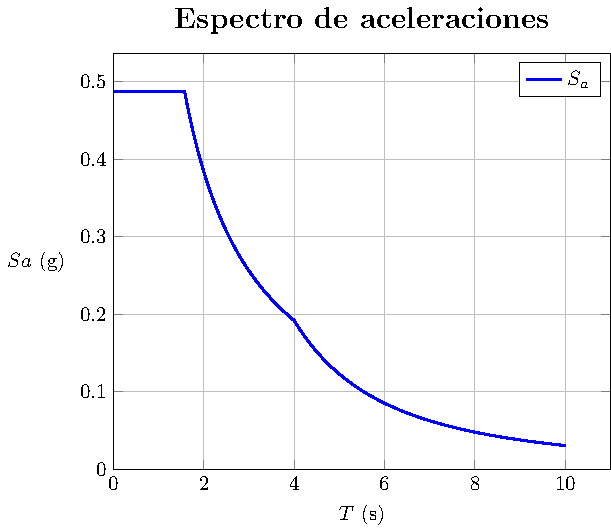
\includegraphics[scale=1.2]{images/Espectro_aceleraciones_DE.pdf}
    \caption{Espectro de aceleraciones }
    \label{fig:ESP}
\end{figure}


 \subsection{Cortante en la base}
 
 El cortante en la base se calcula con la ecuación (A.4.3.1) de la NSR-10 como se muestra a continuación, en donde se tiene que $Sa=0.4875$ (ver sección \ref{secc:espectro y sa}) y el peso del edificio $W=14361.57~kN$ (ver tabla \ref{tab:ResumenWEd})
 
 \begin{equation}
     V_{s}=S_{a}\cdot g \cdot M = 0.4875 \cdot 14361.57~kN= 7001.267~kN
 \end{equation}
 
\subsection{Distribución vertical de la fuerza sísmica}

Teniendo en cuenta la sección \textit{A.4.3.2} se realiza la distribución del cortante sísmico en la base para cada piso de la estructura utilizando el coeficiente $C_{vx}$ que se define de la siguiente manera:

\begin{equation}
    C_{vx}=\frac{m_{x}\cdot h_{x}^{k}}{\sum_{i=1}^{n}(m_{i}\cdot h_{i}^{k})}
\end{equation}
Donde se tiene que el coeficiente \textbf{k}, el cual se relaciona con el periodo fundamental T y para el caso de la estructura tiene un valor de $\mathbf{k=1.0}$ porque el periodo $T_{a}$ es menor a 0.5. A partir de $\mathbf{C_{vx}}$ se obtiene la fuerza sísmica que se le aplica a cada uno de los pisos.
\begin{equation}
    Fx=C_{vx}\cdot V_s
\end{equation}

Al utilizar esta formulación y con los datos obtenidos anteriormente este procedimiento se resume en la siguiente tabla:

% Table generated by Excel2LaTeX from sheet 'W_Edificio'
\begin{table}[H]
  \centering
  
    \begin{tabular}{rrr|c|c|c|r}
    \hline
    \rowcolor[rgb]{ .2,  .247,  .31} \multicolumn{1}{|c|}{\textcolor[rgb]{ 1,  1,  1}{\textbf{Nivel}}} & \multicolumn{1}{c|}{\textcolor[rgb]{ 1,  1,  1}{\textbf{mx (Wx)}}} & \multicolumn{1}{c|}{\textcolor[rgb]{ 1,  1,  1}{\textbf{hx}}} & \textcolor[rgb]{ 1,  1,  1}{\textbf{mxhxk}} & \textcolor[rgb]{ 1,  1,  1}{\textbf{Cvx}} & \textcolor[rgb]{ 1,  1,  1}{\textbf{Fx(kN)}} & \multicolumn{1}{c|}{\textcolor[rgb]{ 1,  1,  1}{\textbf{Vx (kN)}}} \bigstrut\\
    \hline
    \rowcolor[rgb]{ .2,  .247,  .31} \multicolumn{1}{|c|}{\textcolor[rgb]{ 1,  1,  1}{\textbf{Cubierta}}} & \multicolumn{1}{c|}{\cellcolor[rgb]{ 1,  1,  1}3104.45} & \multicolumn{1}{c|}{\cellcolor[rgb]{ 1,  1,  1}12.1} & \cellcolor[rgb]{ 1,  1,  1}37563.86 & \cellcolor[rgb]{ 1,  1,  1}0.354 & \cellcolor[rgb]{ 1,  1,  1}2475.66 & \multicolumn{1}{c|}{\cellcolor[rgb]{ 1,  1,  1}2475.66} \bigstrut\\
    \hline
    \rowcolor[rgb]{ .2,  .247,  .31} \multicolumn{1}{|c|}{\textcolor[rgb]{ 1,  1,  1}{\textbf{4°}}} & \multicolumn{1}{c|}{\cellcolor[rgb]{ 1,  1,  1}3752.37} & \multicolumn{1}{c|}{\cellcolor[rgb]{ 1,  1,  1}9.1} & \cellcolor[rgb]{ 1,  1,  1}34146.60 & \cellcolor[rgb]{ 1,  1,  1}0.321 & \cellcolor[rgb]{ 1,  1,  1}2250.44 & \multicolumn{1}{c|}{\cellcolor[rgb]{ 1,  1,  1}4726.10} \bigstrut\\
    \hline
    \rowcolor[rgb]{ .2,  .247,  .31} \multicolumn{1}{|c|}{\textcolor[rgb]{ 1,  1,  1}{\textbf{3°}}} & \multicolumn{1}{c|}{\cellcolor[rgb]{ 1,  1,  1}3752.37} & \multicolumn{1}{c|}{\cellcolor[rgb]{ 1,  1,  1}6.1} & \cellcolor[rgb]{ 1,  1,  1}22889.48 & \cellcolor[rgb]{ 1,  1,  1}0.215 & \cellcolor[rgb]{ 1,  1,  1}1508.54 & \multicolumn{1}{c|}{\cellcolor[rgb]{ 1,  1,  1}6234.63} \bigstrut\\
    \hline
    \rowcolor[rgb]{ .2,  .247,  .31} \multicolumn{1}{|c|}{\textcolor[rgb]{ 1,  1,  1}{\textbf{2°}}} & \multicolumn{1}{c|}{\cellcolor[rgb]{ 1,  1,  1}3752.37} & \multicolumn{1}{c|}{\cellcolor[rgb]{ 1,  1,  1}3.1} & \cellcolor[rgb]{ 1,  1,  1}11632.36 & \cellcolor[rgb]{ 1,  1,  1}0.109 & \cellcolor[rgb]{ 1,  1,  1}766.63 & \multicolumn{1}{c|}{\cellcolor[rgb]{ 1,  1,  1}7001.27} \bigstrut\\
    \hline
        &     &     & \textbf{106232.31} & \textbf{1.000} & \textbf{7001.27} &  \bigstrut\\
\cline{4-6}    \end{tabular}%
\caption{Distribución vertical de la fuerza sísmica}
  \label{tab:DVFS}%
\end{table}%



\subsection{Torsión accidental}

La torsión accidental se calcula suponiendo que la masa de casa piso está desplazada del centro de masa un 5\% de la longitud máxima en que se está analizando. Estas longitudes máximas se presentan en la tabla \ref{tab:LMAX_TA}

% Table generated by Excel2LaTeX from sheet 'W_Edificio'
\begin{table}[h]
  \centering
 
    \begin{tabular}{|c|c|}
    \hline
    \rowcolor[rgb]{ .2,  .247,  .31} \textcolor[rgb]{ 1,  1,  1}{\textbf{Lx}} & \cellcolor[rgb]{ 1,  1,  1}22.9 \bigstrut\\
    \hline
    \rowcolor[rgb]{ .2,  .247,  .31} \textcolor[rgb]{ 1,  1,  1}{\textbf{Ly}} & \cellcolor[rgb]{ 1,  1,  1}19.2 \bigstrut\\
    \hline
    \rowcolor[rgb]{ .2,  .247,  .31} \textcolor[rgb]{ 1,  1,  1}{\textbf{eax}} & \cellcolor[rgb]{ 1,  1,  1}1.145 \bigstrut\\
    \hline
    \rowcolor[rgb]{ .2,  .247,  .31} \textcolor[rgb]{ 1,  1,  1}{\textbf{eay}} & \cellcolor[rgb]{ 1,  1,  1}0.96 \bigstrut\\
    \hline
    \end{tabular}%
     \caption{Longitudes máximas para torsión accidental}
  \label{tab:LMAX_TA}%
\end{table}%

La torsión accidental se encuentra multiplicando la fuerza horizontal y las longitudes máximas, como se presenta a continuación.
% Table generated by Excel2LaTeX from sheet 'W_Edificio'
\begin{table}[h]
  \centering
  
    \begin{tabular}{|c|c|c|c|}
    \hline
    \rowcolor[rgb]{ .2,  .247,  .31} \textcolor[rgb]{ 1,  1,  1}{\textbf{Nivel}} & \textcolor[rgb]{ 1,  1,  1}{\textbf{Fx (kN)}} & \textcolor[rgb]{ 1,  1,  1}{\textbf{Tx}} & \textcolor[rgb]{ 1,  1,  1}{\textbf{Ty (kN)}} \bigstrut\\
    \hline
    \rowcolor[rgb]{ .2,  .247,  .31} \textcolor[rgb]{ 1,  1,  1}{\textbf{Cubierta}} & \cellcolor[rgb]{ 1,  1,  1}2475.66 & \cellcolor[rgb]{ 1,  1,  1}2376.63 & \cellcolor[rgb]{ 1,  1,  1}2834.63 \bigstrut\\
    \hline
    \rowcolor[rgb]{ .2,  .247,  .31} \textcolor[rgb]{ 1,  1,  1}{\textbf{4°}} & \cellcolor[rgb]{ 1,  1,  1}2250.44 & \cellcolor[rgb]{ 1,  1,  1}2160.42 & \cellcolor[rgb]{ 1,  1,  1}2576.75 \bigstrut\\
    \hline
    \rowcolor[rgb]{ .2,  .247,  .31} \textcolor[rgb]{ 1,  1,  1}{\textbf{3°}} & \cellcolor[rgb]{ 1,  1,  1}1508.54 & \cellcolor[rgb]{ 1,  1,  1}1448.20 & \cellcolor[rgb]{ 1,  1,  1}1727.27 \bigstrut\\
    \hline
    \rowcolor[rgb]{ .2,  .247,  .31} \textcolor[rgb]{ 1,  1,  1}{\textbf{2°}} & \cellcolor[rgb]{ 1,  1,  1}766.63 & \cellcolor[rgb]{ 1,  1,  1}735.97 & \cellcolor[rgb]{ 1,  1,  1}877.80 \bigstrut\\
    \hline
    \end{tabular}%
    \caption{Valores de torsión accidental}
  \label{tab:TorsiónAccidental}%
\end{table}%

\subsection{Irregularidades en planta, altura y por ausencia de redundancia}

\subsubsection{Irregularidades en planta}
\textbf{Tipo 1aP y 1bP- irregularidad torsional e irregularidad torsional extrema}\\

Para determinar si se presenta irregularidad torsional o irregularidad torsional extrema se compara la deriva mayor con la deriva promedio en cada uno de los lados de la estructura como se presenta a continuación:
% Table generated by Excel2LaTeX from sheet 'Irregularidades '
\begin{table}[H]
  \centering
  
    \begin{tabular}{|c|l|r|r|}
\cline{3-4}    \multicolumn{1}{r}{} &     & \multicolumn{1}{c|}{\cellcolor[rgb]{ .2,  .247,  .31}\textcolor[rgb]{ 1,  1,  1}{$\mathbf{\Delta X (m)}$}} & \multicolumn{1}{c|}{\cellcolor[rgb]{ .2,  .247,  .31}\textcolor[rgb]{ 1,  1,  1}{\textbf{$\mathbf{\Delta Y (m)}$}}} \bigstrut\\
    \hline
    \rowcolor[rgb]{ .2,  .247,  .31} \multicolumn{4}{|c|}{\textcolor[rgb]{ 1,  1,  1}{\textbf{A1-A4}}} \bigstrut\\
    \hline
    \multirow{2}[4]{*}{\textbf{CUB}} & Promedio & 0.0217 & 0.0153 \bigstrut\\
\cline{2-4}        & Relación & 1.00 & 1.14 \bigstrut\\
    \hline
    \multirow{2}[4]{*}{\textbf{4}} & Promedio & 0.0285 & 0.0234 \bigstrut\\
\cline{2-4}        & Relación & 1.00 & 1.12 \bigstrut\\
    \hline
    \multirow{2}[4]{*}{\textbf{3}} & Promedio & 0.0297 & 0.0268 \bigstrut\\
\cline{2-4}        & Relación & 1.00 & 1.09 \bigstrut\\
    \hline
    \multirow{2}[4]{*}{\textbf{2}} & Promedio & 0.0168 & 0.0169 \bigstrut\\
\cline{2-4}        & Relación & 1.00 & 1.07 \bigstrut\\
    \hline
    \end{tabular}%
    \caption{Comparación derivas para irregularidad torsional (A1-A4)}
  \label{tab:A1-A4}%
\end{table}%


% Table generated by Excel2LaTeX from sheet 'Irregularidades '
\begin{table}[H]
  \centering
    \begin{tabular}{|c|l|r|r|}
\cline{3-4}    \multicolumn{1}{r}{} &     & \multicolumn{1}{c|}{\cellcolor[rgb]{ .2,  .247,  .31}\textcolor[rgb]{ 1,  1,  1}{\textbf{$\mathbf{\Delta X (m)}$}}} & \multicolumn{1}{c|}{\cellcolor[rgb]{ .2,  .247,  .31}\textcolor[rgb]{ 1,  1,  1}{\textbf{$\mathbf{\Delta Y (m)}$}}} \bigstrut\\
    \hline
    \rowcolor[rgb]{ .2,  .247,  .31} \multicolumn{4}{|c|}{\textcolor[rgb]{ 1,  1,  1}{\textbf{A1-D1}}} \bigstrut\\
    \hline
    \multirow{2}[4]{*}{\textbf{CUB}} & Promedio & 0.0212 & 0.0175 \bigstrut\\
\cline{2-4}        & Relación & 1.02 & 1.00 \bigstrut\\
    \hline
    \multirow{2}[4]{*}{\textbf{4}} & Promedio & 0.0281 & 0.0261 \bigstrut\\
\cline{2-4}        & Relación & 1.02 & 1.00 \bigstrut\\
    \hline
    \multirow{2}[4]{*}{\textbf{3}} & Promedio & 0.0294 & 0.0293 \bigstrut\\
\cline{2-4}        & Relación & 1.01 & 1.00 \bigstrut\\
    \hline
    \multirow{2}[4]{*}{\textbf{2}} & Promedio & 0.0167 & 0.0180 \bigstrut\\
\cline{2-4}        & Relación & 1.00 & 1.00 \bigstrut\\
    \hline
    \end{tabular}%

    \caption{Comparación derivas para irregularidad torsional (A1-D1)}
  \label{tab:A1-D1}%
\end{table}%

% Table generated by Excel2LaTeX from sheet 'Irregularidades '
\begin{table}[H]
  \centering
    \begin{tabular}{|c|l|r|r|}
\cline{3-4}    \multicolumn{1}{r}{} &     & \multicolumn{1}{c|}{\cellcolor[rgb]{ .2,  .247,  .31}\textcolor[rgb]{ 1,  1,  1}{\textbf{$\mathbf{\Delta X (m)}$}}} & \multicolumn{1}{c|}{\cellcolor[rgb]{ .2,  .247,  .31}\textcolor[rgb]{ 1,  1,  1}{\textbf{$\mathbf{\Delta Y (m)}$}}} \bigstrut\\
    \hline
    \rowcolor[rgb]{ .2,  .247,  .31} \multicolumn{4}{|c|}{\textcolor[rgb]{ 1,  1,  1}{\textbf{D1-D4}}} \bigstrut\\
    \hline
    \multirow{2}[4]{*}{\textbf{CUB}} & Promedio & 0.0207 & 0.0153 \bigstrut\\
\cline{2-4}        & Relación & 1.00 & 1.14 \bigstrut\\
    \hline
    \multirow{2}[4]{*}{\textbf{4}} & Promedio & 0.0277 & 0.0234 \bigstrut\\
\cline{2-4}        & Relación & 1.00 & 1.12 \bigstrut\\
    \hline
    \multirow{2}[4]{*}{\textbf{3}} & Promedio & 0.0292 & 0.0268 \bigstrut\\
\cline{2-4}        & Relación & 1.00 & 1.09 \bigstrut\\
    \hline
    \multirow{2}[4]{*}{\textbf{2}} & Promedio & 0.0167 & 0.0169 \bigstrut\\
\cline{2-4}        & Relación & 0.02 & 0.02 \bigstrut\\
    \hline
    \end{tabular}%
    \caption{Comparación derivas para irregularidad torsional (D1-D4)}
  \label{tab:D1-D4}%
\end{table}%

% Table generated by Excel2LaTeX from sheet 'Irregularidades '
\begin{table}[H]
  \centering
    \begin{tabular}{|c|l|r|r|}
\cline{3-4}    \multicolumn{1}{r}{} &     & \multicolumn{1}{c|}{\cellcolor[rgb]{ .2,  .247,  .31}\textcolor[rgb]{ 1,  1,  1}{\textbf{$\mathbf{\Delta X (m)}$}}} & \multicolumn{1}{c|}{\cellcolor[rgb]{ .2,  .247,  .31}\textcolor[rgb]{ 1,  1,  1}{\textbf{$\mathbf{\Delta Y (m)}$}}} \bigstrut\\
    \hline
    \rowcolor[rgb]{ .2,  .247,  .31} \multicolumn{4}{|c|}{\textcolor[rgb]{ 1,  1,  1}{\textbf{D4-A4}}} \bigstrut\\
    \hline
    \multirow{2}[4]{*}{\textbf{CUB}} & Promedio & 0.0212 & 0.0132 \bigstrut\\
\cline{2-4}        & Relación & 1.02 & 1.00 \bigstrut\\
    \hline
    \multirow{2}[4]{*}{\textbf{4}} & Promedio & 0.0281 & 0.0207 \bigstrut\\
\cline{2-4}        & Relación & 1.02 & 1.00 \bigstrut\\
    \hline
    \multirow{2}[4]{*}{\textbf{3}} & Promedio & 0.0294 & 0.0243 \bigstrut\\
\cline{2-4}        & Relación & 1.01 & 1.00 \bigstrut\\
    \hline
    \multirow{2}[4]{*}{\textbf{2}} & Promedio & 0.0167 & 0.0157 \bigstrut\\
\cline{2-4}        & Relación & 1.00 & 1.00 \bigstrut\\
    \hline
    \end{tabular}%
    \caption{Comparación derivas para irregularidad torsional (D4-A4)}
  \label{tab:D4-A4}%
\end{table}%

La máxima relación entre la deriva máxima y la deriva promedio es de 1.14, como este valor es menor a 1.2 se concluye que no se presenta irregularidad torsional.\\

\textbf{Tipo 2P - Retrocesos en las esquinas}\\

De acuerdo a la geometría de la losa se verifica que la estructura no presenta irregularidad por retrocesos en las esquinas, por lo cual el valor de $\phi=1.0$

\textbf{Tipo 3P- Irregularidad del diafragma }\\

Como se muestra en los planos adjuntos a este documento, la estructura presenta diversos vacíos debido al ascensor, la escalera y los ductos. Sin embargo estos son menores al 50\% del área de cada piso, por lo que no se considera la irregularidad de diafragma.

\textbf{Tipo 4P- Desplazamiento de los planos de Acción }\\
No se presentan desplazamientos de los planos de acción porque las columnas transmiten el peso de manera continua desde la cubierta hasta el suelo.\\

\textbf{Tipo 5P- Sistemas no paralelos}
No se presentan sistemas no paralelos en la estructura de acuerdo a la distribución geométrica de los ejes de la estructura.

Una vez verificado los tipos de irregularidades que se presentan se determina un coeficiente de reducción de la capacidad de disipación de energía por irregularidades en planta de $\mathbf{\phi_{p}=1.0}$

\subsubsection{Irregularidades en la altura}

\textbf{Tipo 1aA y 1bA - Piso flexible y Piso flexible extremo}\\
Teniendo en cuenta que la altura del primer piso solo difiere en $10\;cm$ con respecto a la de los demás pisos, no se presenta irregularidad por piso flexible.\\

\textbf{Tipo 2A - Irregularidad en la distribución de masa }\\
 Debido a que la masa de entrepiso no es 1.5 veces mayor que la de cubierta no se presenta este tipo de irregularidad.\\
 
 \textbf{Tipo 3A - Irregularidad geométrica}\\
 De acuerdo a la distribución geométrica del sistema de resistencia sísmica de entrepisos y cubierta no se presenta una dimensión que sea mayor a 1.3 veces  la dimensión del piso adyacente. Por lo que se determina que la estructura no presenta este tipo de irregularidad\\
 
 \textbf{Tipo 4A - Desplazamiento dentro del plano de acción}\\
 Como se menciona anteriormente, las columnas son continuas a lo largo de todos los pisos , por lo que no se presenta este tipo de irregularidad.\\
 
 \textbf{Tipo 5aA y 5bA - Piso débil y piso débil extremo}\\
 
De acuerdo a la geometría de las plantas, la rigidez es similar en todos los pisos, por lo que no se considera irregularidad por piso débil.\\

Como no se presentan irregularidades en altura, se tiene que el coeficiente de reducción de la capacidad de disipación de energía por irregularidades en altura es igual a $\mathbf{\phi_{a}=1}$

\subsubsection{Irregularidades por ausencia de redundancia}


De acuerdo con el numeral A.3.3.8.2 de la NSR-10 no se tiene irregularidad por ausencia de redundancia debido a que no se presenta falta de repetición de elementos estructurales verticales por lo que no hay una pérdida de resistencia a momento en la conexión viga-columna de los dos extremos de la viga mayor al 33\% de la resistencia ante fuerzas horizontales del piso. Adicionalmente, no se produce ningún tipo de irregularidad torsional en planta extrema, por lo cual se considera un valor de $\mathbf{\phi_{r}=1}$

 
 
 


\subsection{Coeficiente de capacidad de disipación de energía, $R_{0}$}

De acuerdo al reglamento NSR-10, específicamente a la tabla \textit{A.3-3}, el tipo de sistema estructural y la zona del proyecto se determina que para una estructura de pórtico resistente a momentos en concreto reforzado en Bogotá, una zona de amenaza sísmica intermedia se tiene que $R_0=5.0$ y $\Omega=3.0$ teniendo en cuenta que la edificación está dentro de la categoría de capacidad moderada de disipación de energía (DMO).

\subsection{Capacidad de disipación de energía R}

Teniendo en cuenta la sección \textit{A.3.1.1} se calcula el coeficiente capacidad de disipación de energía teniendo en cuenta los coeficientes de reducción según sean aplicables al caso.

\begin{equation*}
    R=\phi_{a}\cdot \phi_{p}\cdot \phi_{r}\cdot R_{0}=1\cdot 1\cdot 1\cdot 5=\mathbf{5}
\end{equation*}

%AJUSTAR ESTO DE ACUERDO CON EL NUEVO MODELO
\subsection{Cálculo del período real de la estructura}
 El periodo fundamental de vibración de la estructura.

\begin{equation}
    T = 2\pi \sqrt{\frac{\displaystyle\sum_{i=1}^{n}\left( m_{i} \cdot  \delta_{i}^2\right)}{\displaystyle\sum_{i=1}^{n}\left(f_{i}  \cdot \delta_{i}\right)}}
    \label{eq:CalcT}
\end{equation}

El periodo fundamental se calcula  para los desplazamientos en x y en y, los cuales corresponden a los desplazamientos causados por las fuerzas sísmicas \textbf{F}. Los resultados obtenidos a partir de la aplicación de la ecuación \ref{eq:CalcT} son los siguientes:
\begin{table}[h]
\centering
\resizebox{\linewidth}{!}{
\begin{tabular}{|c|c|c|c|c|c|c|c|c|cc} 
\hhline{~----------|}
\multicolumn{1}{c|}{}                                                    & {\cellcolor[rgb]{0.243,0.243,0.243}}\textcolor{white}{\textbf{$m (Ton)$}} & {\cellcolor[rgb]{0.243,0.243,0.243}}\textcolor{white}{\textbf{$FX=FY (KN)$}} & {\cellcolor[rgb]{0.243,0.243,0.243}}\textcolor{white}{\textbf{$\delta x (m)$}} & {\cellcolor[rgb]{0.243,0.243,0.243}}\textcolor{white}{\textbf{$ \delta y (m)$}} & {\cellcolor[rgb]{0.243,0.243,0.243}}\textcolor{white}{\textbf{$F \cdot \delta x$}} & {\cellcolor[rgb]{0.243,0.243,0.243}}\textcolor{white}{\textbf{$F \cdot \delta y$}} & {\cellcolor[rgb]{0.243,0.243,0.243}}\textcolor{white}{\textbf{$m \cdot \delta x^2$}} & {\cellcolor[rgb]{0.243,0.243,0.243}}\textcolor{white}{\textbf{$m \cdot \delta y²$}} & \multicolumn{1}{c|}{{\cellcolor[rgb]{0.243,0.243,0.243}}\textcolor{white}{\textbf{$Tx$}}} & \multicolumn{1}{c|}{{\cellcolor[rgb]{0.243,0.243,0.243}}\textcolor{white}{\textbf{$Ty$}}}  \\ 
\hline
{\cellcolor[rgb]{0.255,0.255,0.255}}\textbf{\textcolor{white}{Cubierta}} & 316.458
                                               & 2475.656
                                                                     & 0.089
                                                                          & 0.074
                                                                           & 220.786
                                                                            & 182.642
                                                                            & 2.517
                                                                                & 1.722
                                                                               & \multicolumn{1}{c|}{{\cellcolor[rgb]{1,0.8,0.431}}\textbf{0.723}}                         & \multicolumn{1}{c|}{{\cellcolor[rgb]{1,0.8,0.431}}\textbf{0.620}}                          \\ 
\hline
{\cellcolor[rgb]{0.255,0.255,0.255}}\textbf{\textcolor{white}{Piso 4}}   & 382.505
                                                                   & 2250.440
                                                                     & 0.069
                                                                          & 0.060
                                                                           & 155.942
                                                                            & 135.735
                                                                           & 1.837
                                                                                & 1.392
                                                                              &                                                                                           &                                                                                            \\ 
\hhline{|---------~~}
{\cellcolor[rgb]{0.255,0.255,0.255}}\textbf{\textcolor{white}{Piso 3}}   & 382.505
                                                                   & 1508.537
                                                                     & 0.043                                                                          & 0.039
                                                                          & 64.900
                                                                             & 59.320
                                                                             & 0.708
                                                                                & 0.591
                                                                              &                                                                                           &                                                                                            \\ 
\hhline{|---------~~}
{\cellcolor[rgb]{0.255,0.255,0.255}}\textbf{\textcolor{white}{Piso 2}}   & 382.505
                                                                   & 766.634
                                                                     & 0.016                                                                          & 0.015                                                                           & 11.933
                                                                            & 11.688
                                                                            & 0.093
                                                                               & 0.089
                                                                              &                                                                                           &                                                                                            \\ 
\hhline{|---------~~}
{\cellcolor[rgb]{0.255,0.255,0.255}}\textbf{\textcolor{white}{Total}}    & 1463.973
                                                                 & \multicolumn{1}{c}{}                                                         & \multicolumn{1}{c}{}                                                           &                                                                                 & 453.561
                                                                            & 389.385
                                                                            & 5.154
                                                                                & 3.794
                                                                              & \multicolumn{1}{l}{}                                                                      & \multicolumn{1}{l}{}                                                                       \\
\hhline{|--~~~----~~}
\end{tabular}}
\caption{Cálculo del periodo fundamental de la estructura en x y en y}
\label{tab:CALCT}
\end{table}

De acuerdo con la sección A.4.2 el valor del periodo fundamental de la edificación \textbf{T} debe ser menor a $ \mathbf{C_{u} T_{a}} $, en donde $Cu$ se obtiene como se muestra en (\ref{eq:C_u}), y este tiene como valor mínimo 1.2

\begin{equation}
    C_{u}=1.75-A_{v}\cdot F_{v} =1.75-0.2 \cdot 3.20 =0.98 < 1.2 \Rightarrow C_{u}=1.2
    \label{eq:C_u}
\end{equation}

Como se observa en la tabla \ref{tab:CALCT}, se obtiene un periodo de \textbf{0.723 s} y \textbf{0.62 s} en x y en y respectivamente. Estos valores son mayores a $\mathbf{C_{u}T_{a}}$, sin embargo no se considera rigidizar la estructura porque el valor de la aceleración es mayor a la experimentada con el periodo actual de la estructura y con esta se cumplen derivas.

\section{Control de la deriva}

La sección \textit{A.6} de la NSR establece los requisitos necesarios para la deriva, dentro de los cuales se especifica que el máximo valor permitido corresponde a 1\% para estructuras de concreto reforzado. El método utilizado de cálculo consiste en la modelación de la estructura en el programa SAP2000 especificando un diafragma rígido en cada piso se calculan las derivas y mediante la siguiente ecuación se verifica que estas estén dentro del rango permisible.

\begin{equation}
    \Delta^{i}_{max}=\sqrt{\sum_{j=1}^{2}(\delta^{i}_{tot,j}-\delta^{i-1}_{tot,j})^{2}}
\end{equation}

 
\subsection{Combinaciones de carga para verificación de derivas}

Las combinaciones utilizadas para la verificación de derivas se muestran a continuación, teniendo en cuenta que $D$ es carga muerta, $L$ es carga viva, $F_{si}$ es la fuerza sísmica en i y $T_i$ es la torsión accidental en i

\begin{itemize}
    \item $D+L+F_{sx}+Tx$
    \item $D+L+F_{sx}-Tx$
    \item $D+L-F_{sx}+Tx$
    \item $D+L-F_{sx}-Tx$
    \item $D+L+F_{sy}+Ty$
    \item $D+L+F_{sy}-Ty$
    \item $D+L-F_{sy}+Ty$
    \item $D+L-F_{sy}-Ty$
\end{itemize}
%AJUSTAR DERIVAS DE ACUERDO AL NUEVO MODELO 
\subsection{Verificación de derivas}

% Table generated by Excel2LaTeX from sheet 'DERIVAS DEF.'
\begin{table}[H]
  \centering
    \scalebox{0.7}{\begin{tabular}{|c|c|c|c|c|c|c|c|c|}
    \hline
    \rowcolor[rgb]{ 0,  .69,  .941} \multicolumn{9}{|c|}{\textbf{A1}} \bigstrut\\
    \hline
    \rowcolor[rgb]{ .8,  1,  1} \textbf{Piso} & \textbf{Combinación} & \textbf{U1 (m)} & \textbf{U2 (m)} & \textbf{$\Delta X (m)$} & \textbf{$\Delta Y (m)$} & \textbf{$\Delta$ Total} & \textbf{$\Delta$ perm} &  \bigstrut\\
\cline{1-8}   \rowcolor[rgb]{ .8,  1,  1}       &       &       &       &       &       &       &       &\multirow{-2}[4]{*}{\textbf{Criterio}}  \bigstrut\\
    \hline
     Cubierta & D+L+FSX+TX & 0.0847 & -0.0064 & 0.0193 & -0.0010 & 0.019 & 0.030 & \cellcolor[rgb]{ .776,  .937,  .808}\textcolor[rgb]{ 0,  .38,  0}{OK} \bigstrut\\
    \hline
    P4  & D+L+FSX+TX & 0.0654 & -0.0054 & 0.0250 & -0.0018 & 0.025 & 0.030 & \cellcolor[rgb]{ .776,  .937,  .808}\textcolor[rgb]{ 0,  .38,  0}{OK} \bigstrut\\
    \hline
    P3  & D+L+FSX+TX & 0.0404 & -0.0036 & 0.0259 & -0.0022 & 0.026 & 0.030 & \cellcolor[rgb]{ .776,  .937,  .808}\textcolor[rgb]{ 0,  .38,  0}{OK} \bigstrut\\
    \hline
    P2  & D+L+FSX+TX & 0.0145 & -0.0014 & 0.0145 & -0.0014 & 0.015 & 0.031 & \cellcolor[rgb]{ .776,  .937,  .808}\textcolor[rgb]{ 0,  .38,  0}{OK} \bigstrut\\
    \hline
    \multicolumn{1}{|r}{} & \multicolumn{1}{r}{} & \multicolumn{1}{r}{} & \multicolumn{1}{r}{} & \multicolumn{1}{r}{} & \multicolumn{1}{r}{} & \multicolumn{1}{r}{} & \multicolumn{1}{r}{} &  \bigstrut\\
    \hline
    Cubierta & D+L+FSX-TX & 0.0968 & 0.0091 & 0.0217 & 0.0021 & 0.022 & 0.030 & \cellcolor[rgb]{ .776,  .937,  .808}\textcolor[rgb]{ 0,  .38,  0}{OK} \bigstrut\\
    \hline
    P4  & D+L+FSX-TX & 0.0750 & 0.0070 & 0.0285 & 0.0027 & 0.029 & 0.030 & \cellcolor[rgb]{ .776,  .937,  .808}\textcolor[rgb]{ 0,  .38,  0}{OK} \bigstrut\\
    \hline
    P3  & D+L+FSX-TX & 0.0465 & 0.0042 & 0.0297 & 0.0027 & 0.030 & 0.030 & \cellcolor[rgb]{ .776,  .937,  .808}\textcolor[rgb]{ 0,  .38,  0}{OK} \bigstrut\\
    \hline
    P2  & D+L+FSX-TX & 0.0168 & 0.0015 & 0.0168 & 0.0015 & 0.017 & 0.031 & \cellcolor[rgb]{ .776,  .937,  .808}\textcolor[rgb]{ 0,  .38,  0}{OK} \bigstrut\\
    \hline
    \multicolumn{1}{|r}{} & \multicolumn{1}{r}{} & \multicolumn{1}{r}{} & \multicolumn{1}{r}{} & \multicolumn{1}{r}{} & \multicolumn{1}{r}{} & \multicolumn{1}{r}{} & \multicolumn{1}{r}{} &  \bigstrut\\
    \hline
    Cubierta & D+L+FSY+TY & -0.0002 & 0.0724 & 0.0003 & 0.0138 & 0.014 & 0.030 & \cellcolor[rgb]{ .776,  .937,  .808}\textcolor[rgb]{ 0,  .38,  0}{OK} \bigstrut\\
    \hline
    P4  & D+L+FSY+TY & -0.0006 & 0.0587 & 0.0001 & 0.0207 & 0.021 & 0.030 & \cellcolor[rgb]{ .776,  .937,  .808}\textcolor[rgb]{ 0,  .38,  0}{OK} \bigstrut\\
    \hline
    P3  & D+L+FSY+TY & -0.0007 & 0.0379 & -0.0003 & 0.0234 & 0.023 & 0.030 & \cellcolor[rgb]{ .776,  .937,  .808}\textcolor[rgb]{ 0,  .38,  0}{OK} \bigstrut\\
    \hline
    P2  & D+L+FSY+TY & -0.0004 & 0.0146 & -0.0004 & 0.0146 & 0.015 & 0.031 & \cellcolor[rgb]{ .776,  .937,  .808}\textcolor[rgb]{ 0,  .38,  0}{OK} \bigstrut\\
    \hline
    \multicolumn{1}{|r}{} & \multicolumn{1}{r}{} & \multicolumn{1}{r}{} & \multicolumn{1}{r}{} & \multicolumn{1}{r}{} & \multicolumn{1}{r}{} & \multicolumn{1}{r}{} & \multicolumn{1}{r}{} &  \bigstrut\\
    \hline
    Cubierta & D+L+FSY-TY & 0.0142 & 0.0909 & 0.0032 & 0.0175 & 0.018 & 0.030 & \cellcolor[rgb]{ .776,  .937,  .808}\textcolor[rgb]{ 0,  .38,  0}{OK} \bigstrut\\
    \hline
    P4  & D+L+FSY-TY & 0.0109 & 0.0735 & 0.0043 & 0.0261 & 0.026 & 0.030 & \cellcolor[rgb]{ .776,  .937,  .808}\textcolor[rgb]{ 0,  .38,  0}{OK} \bigstrut\\
    \hline
    P3  & D+L+FSY-TY & 0.0066 & 0.0473 & 0.0043 & 0.0293 & 0.030 & 0.030 & \cellcolor[rgb]{ .776,  .937,  .808}\textcolor[rgb]{ 0,  .38,  0}{OK} \bigstrut\\
    \hline
    P2  & D+L+FSY-TY & 0.0023 & 0.0180 & 0.0023 & 0.0180 & 0.018 & 0.031 & \cellcolor[rgb]{ .776,  .937,  .808}\textcolor[rgb]{ 0,  .38,  0}{OK} \bigstrut\\
    \hline
    \multicolumn{1}{|r}{} & \multicolumn{1}{r}{} & \multicolumn{1}{r}{} & \multicolumn{1}{r}{} & \multicolumn{1}{r}{} & \multicolumn{1}{r}{} & \multicolumn{1}{r}{} & \multicolumn{1}{r}{} &  \bigstrut\\
    \hline
    Cubierta & D+L-FSX+TX & -0.0962 & -0.0096 & -0.0215 & -0.0023 & 0.022 & 0.030 & \cellcolor[rgb]{ .776,  .937,  .808}\textcolor[rgb]{ 0,  .38,  0}{OK} \bigstrut\\
    \hline
    P4  & D+L-FSX+TX & -0.0747 & -0.0073 & -0.0284 & -0.0029 & 0.029 & 0.030 & \cellcolor[rgb]{ .776,  .937,  .808}\textcolor[rgb]{ 0,  .38,  0}{OK} \bigstrut\\
    \hline
    P3  & D+L-FSX+TX & -0.0463 & -0.0044 & -0.0296 & -0.0029 & 0.030 & 0.030 & \cellcolor[rgb]{ .776,  .937,  .808}\textcolor[rgb]{ 0,  .38,  0}{OK} \bigstrut\\
    \hline
    P2  & D+L-FSX+TX & -0.0167 & -0.0016 & -0.0167 & -0.0016 & 0.017 & 0.031 & \cellcolor[rgb]{ .776,  .937,  .808}\textcolor[rgb]{ 0,  .38,  0}{OK} \bigstrut\\
    \hline
    \multicolumn{1}{|r}{} & \multicolumn{1}{r}{} & \multicolumn{1}{r}{} & \multicolumn{1}{r}{} & \multicolumn{1}{r}{} & \multicolumn{1}{r}{} & \multicolumn{1}{r}{} & \multicolumn{1}{r}{} &  \bigstrut\\
    \hline
    Cubierta & D+L-FSX-TX & -0.0841 & 0.0059 & -0.0191 & 0.0008 & 0.019 & 0.030 & \cellcolor[rgb]{ .776,  .937,  .808}\textcolor[rgb]{ 0,  .38,  0}{OK} \bigstrut\\
    \hline
    P4  & D+L-FSX-TX & -0.0650 & 0.0051 & -0.0249 & 0.0016 & 0.025 & 0.030 & \cellcolor[rgb]{ .776,  .937,  .808}\textcolor[rgb]{ 0,  .38,  0}{OK} \bigstrut\\
    \hline
    P3  & D+L-FSX-TX & -0.0402 & 0.0034 & -0.0257 & 0.0021 & 0.026 & 0.030 & \cellcolor[rgb]{ .776,  .937,  .808}\textcolor[rgb]{ 0,  .38,  0}{OK} \bigstrut\\
    \hline
    P2  & D+L-FSX-TX & -0.0144 & 0.0014 & -0.0144 & 0.0014 & 0.015 & 0.031 & \cellcolor[rgb]{ .776,  .937,  .808}\textcolor[rgb]{ 0,  .38,  0}{OK} \bigstrut\\
    \hline
    \multicolumn{1}{|r}{} & \multicolumn{1}{r}{} & \multicolumn{1}{r}{} & \multicolumn{1}{r}{} & \multicolumn{1}{r}{} & \multicolumn{1}{r}{} & \multicolumn{1}{r}{} & \multicolumn{1}{r}{} &  \bigstrut\\
    \hline
    Cubierta & D+L-FSY+TY & -0.0136 & -0.0915 & -0.0031 & -0.0176 & 0.018 & 0.030 & \cellcolor[rgb]{ .776,  .937,  .808}\textcolor[rgb]{ 0,  .38,  0}{OK} \bigstrut\\
    \hline
    P4  & D+L-FSY+TY & -0.0105 & -0.0738 & -0.0041 & -0.0263 & 0.027 & 0.030 & \cellcolor[rgb]{ .776,  .937,  .808}\textcolor[rgb]{ 0,  .38,  0}{OK} \bigstrut\\
    \hline
    P3  & D+L-FSY+TY & -0.0064 & -0.0475 & -0.0042 & -0.0294 & 0.030 & 0.030 & \cellcolor[rgb]{ .776,  .937,  .808}\textcolor[rgb]{ 0,  .38,  0}{OK} \bigstrut\\
    \hline
    P2  & D+L-FSY+TY & -0.0022 & -0.0181 & -0.0022 & -0.0181 & 0.018 & 0.031 & \cellcolor[rgb]{ .776,  .937,  .808}\textcolor[rgb]{ 0,  .38,  0}{OK} \bigstrut\\
    \hline
    \multicolumn{1}{|r}{} & \multicolumn{1}{r}{} & \multicolumn{1}{r}{} & \multicolumn{1}{r}{} & \multicolumn{1}{r}{} & \multicolumn{1}{r}{} & \multicolumn{1}{r}{} & \multicolumn{1}{r}{} &  \bigstrut\\
    \hline
    Cubierta & D+L-FSY-TY & 0.0008 & -0.0730 & -0.0001 & -0.0139 & 0.014 & 0.030 & \cellcolor[rgb]{ .776,  .937,  .808}\textcolor[rgb]{ 0,  .38,  0}{OK} \bigstrut\\
    \hline
    P4  & D+L-FSY-TY & 0.0010 & -0.0590 & 0.0001 & -0.0209 & 0.021 & 0.030 & \cellcolor[rgb]{ .776,  .937,  .808}\textcolor[rgb]{ 0,  .38,  0}{OK} \bigstrut\\
    \hline
    P3  & D+L-FSY-TY & 0.0009 & -0.0381 & 0.0004 & -0.0235 & 0.024 & 0.030 & \cellcolor[rgb]{ .776,  .937,  .808}\textcolor[rgb]{ 0,  .38,  0}{OK} \bigstrut\\
    \hline
    P2  & D+L-FSY-TY & 0.0005 & -0.0146 & 0.0005 & -0.0146 & 0.015 & 0.031 & \cellcolor[rgb]{ .776,  .937,  .808}\textcolor[rgb]{ 0,  .38,  0}{OK} \bigstrut\\
    \hline
    \end{tabular}}%
  \caption{Verificación de derivas columna A1}
  \label{tab:VDA1}%
\end{table}%

% Table generated by Excel2LaTeX from sheet 'DERIVAS DEF.'
\begin{table}[H]
  \centering
    \scalebox{0.7}{\begin{tabular}{|c|c|c|c|c|c|c|c|c|}
    \hline
    \rowcolor[rgb]{ 0,  .69,  .941} \multicolumn{9}{|c|}{\textbf{A4}} \bigstrut\\
    \hline
    \rowcolor[rgb]{ .8,  1,  1} \textbf{Piso} & \textbf{OutputCase} & \textbf{U1 (m)} & \textbf{U2 (m)} & \textbf{$\Delta X (m)$} & \textbf{$\Delta Y (m)$} & \textbf{$\Delta Total$} & \textbf{$\Delta perm$} &  \bigstrut\\
\cline{1-8}    \rowcolor[rgb]{ .8,  1,  1}       &       &       &       &       &       &       &       & \multirow{-2}[4]{*}{\textbf{Criterio}} \bigstrut\\
    \hline
     Cubierta & D+L+FSX+TX & 0.0847 & 0.0053 & 0.0193 & 0.0007 & 0.019 & 0.030 & \cellcolor[rgb]{ .776,  .937,  .808}\textcolor[rgb]{ 0,  .38,  0}{OK} \bigstrut\\
    \hline
    P4  & D+L+FSX+TX & 0.0654 & 0.0046 & 0.0250 & 0.0014 & 0.025 & 0.030 & \cellcolor[rgb]{ .776,  .937,  .808}\textcolor[rgb]{ 0,  .38,  0}{OK} \bigstrut\\
    \hline
    P3  & D+L+FSX+TX & 0.0404 & 0.0031 & 0.0259 & 0.0019 & 0.026 & 0.030 & \cellcolor[rgb]{ .776,  .937,  .808}\textcolor[rgb]{ 0,  .38,  0}{OK} \bigstrut\\
    \hline
    P2  & D+L+FSX+TX & 0.0145 & 0.0013 & 0.0145 & 0.0013 & 0.015 & 0.031 & \cellcolor[rgb]{ .776,  .937,  .808}\textcolor[rgb]{ 0,  .38,  0}{OK} \bigstrut\\
    \hline
    \multicolumn{1}{|r}{} & \multicolumn{1}{r}{} & \multicolumn{1}{r}{} & \multicolumn{1}{r}{} & \multicolumn{1}{r}{} & \multicolumn{1}{r}{} & \multicolumn{1}{r}{} & \multicolumn{1}{r}{} &  \bigstrut\\
    \hline
    Cubierta & D+L+FSX-TX & 0.0968 & -0.0084 & 0.0217 & -0.0020 & 0.022 & 0.030 & \cellcolor[rgb]{ .776,  .937,  .808}\textcolor[rgb]{ 0,  .38,  0}{OK} \bigstrut\\
    \hline
    P4  & D+L+FSX-TX & 0.0750 & -0.0064 & 0.0285 & -0.0025 & 0.029 & 0.030 & \cellcolor[rgb]{ .776,  .937,  .808}\textcolor[rgb]{ 0,  .38,  0}{OK} \bigstrut\\
    \hline
    P3  & D+L+FSX-TX & 0.0465 & -0.0039 & 0.0297 & -0.0025 & 0.030 & 0.030 & \cellcolor[rgb]{ .776,  .937,  .808}\textcolor[rgb]{ 0,  .38,  0}{OK} \bigstrut\\
    \hline
    P2  & D+L+FSX-TX & 0.0168 & -0.0014 & 0.0168 & -0.0014 & 0.017 & 0.031 & \cellcolor[rgb]{ .776,  .937,  .808}\textcolor[rgb]{ 0,  .38,  0}{OK} \bigstrut\\
    \hline
    \multicolumn{1}{|r}{} & \multicolumn{1}{r}{} & \multicolumn{1}{r}{} & \multicolumn{1}{r}{} & \multicolumn{1}{r}{} & \multicolumn{1}{r}{} & \multicolumn{1}{r}{} & \multicolumn{1}{r}{} &  \bigstrut\\
    \hline
    Cubierta & D+L+FSY+TY & -0.0002 & 0.0739 & 0.0003 & 0.0132 & 0.013 & 0.030 & \cellcolor[rgb]{ .776,  .937,  .808}\textcolor[rgb]{ 0,  .38,  0}{OK} \bigstrut\\
    \hline
    P4  & D+L+FSY+TY & -0.0006 & 0.0607 & 0.0001 & 0.0207 & 0.021 & 0.030 & \cellcolor[rgb]{ .776,  .937,  .808}\textcolor[rgb]{ 0,  .38,  0}{OK} \bigstrut\\
    \hline
    P3  & D+L+FSY+TY & -0.0007 & 0.0400 & -0.0003 & 0.0243 & 0.024 & 0.030 & \cellcolor[rgb]{ .776,  .937,  .808}\textcolor[rgb]{ 0,  .38,  0}{OK} \bigstrut\\
    \hline
    P2  & D+L+FSY+TY & -0.0004 & 0.0157 & -0.0004 & 0.0157 & 0.016 & 0.031 & \cellcolor[rgb]{ .776,  .937,  .808}\textcolor[rgb]{ 0,  .38,  0}{OK} \bigstrut\\
    \hline
    \multicolumn{1}{|r}{} & \multicolumn{1}{r}{} & \multicolumn{1}{r}{} & \multicolumn{1}{r}{} & \multicolumn{1}{r}{} & \multicolumn{1}{r}{} & \multicolumn{1}{r}{} & \multicolumn{1}{r}{} &  \bigstrut\\
    \hline
    Cubierta & D+L+FSY-TY & 0.0142 & 0.0576 & 0.0032 & 0.0100 & 0.010 & 0.030 & \cellcolor[rgb]{ .776,  .937,  .808}\textcolor[rgb]{ 0,  .38,  0}{OK} \bigstrut\\
    \hline
    P4  & D+L+FSY-TY & 0.0109 & 0.0476 & 0.0043 & 0.0160 & 0.017 & 0.030 & \cellcolor[rgb]{ .776,  .937,  .808}\textcolor[rgb]{ 0,  .38,  0}{OK} \bigstrut\\
    \hline
    P3  & D+L+FSY-TY & 0.0066 & 0.0316 & 0.0043 & 0.0191 & 0.020 & 0.030 & \cellcolor[rgb]{ .776,  .937,  .808}\textcolor[rgb]{ 0,  .38,  0}{OK} \bigstrut\\
    \hline
    P2  & D+L+FSY-TY & 0.0023 & 0.0125 & 0.0023 & 0.0125 & 0.013 & 0.031 & \cellcolor[rgb]{ .776,  .937,  .808}\textcolor[rgb]{ 0,  .38,  0}{OK} \bigstrut\\
    \hline
    \multicolumn{1}{|r}{} & \multicolumn{1}{r}{} & \multicolumn{1}{r}{} & \multicolumn{1}{r}{} & \multicolumn{1}{r}{} & \multicolumn{1}{r}{} & \multicolumn{1}{r}{} & \multicolumn{1}{r}{} &  \bigstrut\\
    \hline
    Cubierta & D+L-FSX+TX & -0.0962 & 0.0081 & -0.0215 & 0.0019 & 0.022 & 0.030 & \cellcolor[rgb]{ .776,  .937,  .808}\textcolor[rgb]{ 0,  .38,  0}{OK} \bigstrut\\
    \hline
    P4  & D+L-FSX+TX & -0.0747 & 0.0062 & -0.0284 & 0.0024 & 0.028 & 0.030 & \cellcolor[rgb]{ .776,  .937,  .808}\textcolor[rgb]{ 0,  .38,  0}{OK} \bigstrut\\
    \hline
    P3  & D+L-FSX+TX & -0.0463 & 0.0038 & -0.0296 & 0.0024 & 0.030 & 0.030 & \cellcolor[rgb]{ .776,  .937,  .808}\textcolor[rgb]{ 0,  .38,  0}{OK} \bigstrut\\
    \hline
    P2  & D+L-FSX+TX & -0.0167 & 0.0014 & -0.0167 & 0.0014 & 0.017 & 0.031 & \cellcolor[rgb]{ .776,  .937,  .808}\textcolor[rgb]{ 0,  .38,  0}{OK} \bigstrut\\
    \hline
    \multicolumn{1}{|r}{} & \multicolumn{1}{r}{} & \multicolumn{1}{r}{} & \multicolumn{1}{r}{} & \multicolumn{1}{r}{} & \multicolumn{1}{r}{} & \multicolumn{1}{r}{} & \multicolumn{1}{r}{} &  \bigstrut\\
    \hline
    Cubierta & D+L-FSX-TX & -0.0841 & -0.0056 & -0.0191 & -0.0008 & 0.019 & 0.030 & \cellcolor[rgb]{ .776,  .937,  .808}\textcolor[rgb]{ 0,  .38,  0}{OK} \bigstrut\\
    \hline
    P4  & D+L-FSX-TX & -0.0650 & -0.0048 & -0.0249 & -0.0015 & 0.025 & 0.030 & \cellcolor[rgb]{ .776,  .937,  .808}\textcolor[rgb]{ 0,  .38,  0}{OK} \bigstrut\\
    \hline
    P3  & D+L-FSX-TX & -0.0402 & -0.0032 & -0.0257 & -0.0019 & 0.026 & 0.030 & \cellcolor[rgb]{ .776,  .937,  .808}\textcolor[rgb]{ 0,  .38,  0}{OK} \bigstrut\\
    \hline
    P2  & D+L-FSX-TX & -0.0144 & -0.0013 & -0.0144 & -0.0013 & 0.014 & 0.031 & \cellcolor[rgb]{ .776,  .937,  .808}\textcolor[rgb]{ 0,  .38,  0}{OK} \bigstrut\\
    \hline
    \multicolumn{1}{|r}{} & \multicolumn{1}{r}{} & \multicolumn{1}{r}{} & \multicolumn{1}{r}{} & \multicolumn{1}{r}{} & \multicolumn{1}{r}{} & \multicolumn{1}{r}{} & \multicolumn{1}{r}{} &  \bigstrut\\
    \hline
    Cubierta & D+L-FSY+TY & -0.0136 & -0.0579 & -0.0031 & -0.0101 & 0.011 & 0.030 & \cellcolor[rgb]{ .776,  .937,  .808}\textcolor[rgb]{ 0,  .38,  0}{OK} \bigstrut\\
    \hline
    P4  & D+L-FSY+TY & -0.0105 & -0.0478 & -0.0041 & -0.0161 & 0.017 & 0.030 & \cellcolor[rgb]{ .776,  .937,  .808}\textcolor[rgb]{ 0,  .38,  0}{OK} \bigstrut\\
    \hline
    P3  & D+L-FSY+TY & -0.0064 & -0.0317 & -0.0042 & -0.0191 & 0.020 & 0.030 & \cellcolor[rgb]{ .776,  .937,  .808}\textcolor[rgb]{ 0,  .38,  0}{OK} \bigstrut\\
    \hline
    P2  & D+L-FSY+TY & -0.0022 & -0.0126 & -0.0022 & -0.0126 & 0.013 & 0.031 & \cellcolor[rgb]{ .776,  .937,  .808}\textcolor[rgb]{ 0,  .38,  0}{OK} \bigstrut\\
    \hline
    \multicolumn{1}{|r}{} & \multicolumn{1}{r}{} & \multicolumn{1}{r}{} & \multicolumn{1}{r}{} & \multicolumn{1}{r}{} & \multicolumn{1}{r}{} & \multicolumn{1}{r}{} & \multicolumn{1}{r}{} &  \bigstrut\\
    \hline
    Cubierta & D+L-FSY-TY & 0.0008 & -0.0742 & -0.0001 & -0.0133 & 0.013 & 0.030 & \cellcolor[rgb]{ .776,  .937,  .808}\textcolor[rgb]{ 0,  .38,  0}{OK} \bigstrut\\
    \hline
    P4  & D+L-FSY-TY & 0.0010 & -0.0609 & 0.0001 & -0.0208 & 0.021 & 0.030 & \cellcolor[rgb]{ .776,  .937,  .808}\textcolor[rgb]{ 0,  .38,  0}{OK} \bigstrut\\
    \hline
    P3  & D+L-FSY-TY & 0.0009 & -0.0401 & 0.0004 & -0.0243 & 0.024 & 0.030 & \cellcolor[rgb]{ .776,  .937,  .808}\textcolor[rgb]{ 0,  .38,  0}{OK} \bigstrut\\
    \hline
    P2  & D+L-FSY-TY & 0.0005 & -0.0157 & 0.0005 & -0.0157 & 0.016 & 0.031 & \cellcolor[rgb]{ .776,  .937,  .808}\textcolor[rgb]{ 0,  .38,  0}{OK} \bigstrut\\
    \hline
    \end{tabular}}%
  \caption{Verificación de derivas columna A4}
  \label{tab:VDA4}%
\end{table}%

% Table generated by Excel2LaTeX from sheet 'DERIVAS DEF.'
\begin{table}[H]
  \centering
    \scalebox{0.7}{\begin{tabular}{|c|c|c|c|c|c|c|c|c|}
    \hline
    \rowcolor[rgb]{ 0,  .69,  .941} \multicolumn{9}{|c|}{\textbf{D1}} \bigstrut\\
    \hline
    \rowcolor[rgb]{ .8,  1,  1} \textbf{Piso} & \textbf{OutputCase} & \textbf{U1 (m)} & \textbf{U2 (m)} & \textbf{$\Delta X (m)$} & \textbf{$\Delta Y (m)$} & \textbf{$\Delta Total$} & \textbf{$\Delta perm$} &  \bigstrut\\
\cline{1-8}    \rowcolor[rgb]{ .8,  1,  1}       &       &       &       &       &       &       &       &\multirow{-2}[4]{*}{\textbf{Criterio}}  \bigstrut\\
    \hline
    Cubierta & D+L+FSX+TX & 0.0942 & -0.0064 & 0.0207 & -0.0010 & 0.021 & 0.030 & \cellcolor[rgb]{ .776,  .937,  .808}\textcolor[rgb]{ 0,  .38,  0}{OK} \bigstrut\\
    \hline
    P4  & D+L+FSX+TX & 0.0735 & -0.0054 & 0.0277 & -0.0018 & 0.028 & 0.030 & \cellcolor[rgb]{ .776,  .937,  .808}\textcolor[rgb]{ 0,  .38,  0}{OK} \bigstrut\\
    \hline
    P3  & D+L+FSX+TX & 0.0459 & -0.0036 & 0.0292 & -0.0022 & 0.029 & 0.030 & \cellcolor[rgb]{ .776,  .937,  .808}\textcolor[rgb]{ 0,  .38,  0}{OK} \bigstrut\\
    \hline
    P2  & D+L+FSX+TX & 0.0167 & -0.0014 & 0.0167 & -0.0014 & 0.017 & 0.031 & \cellcolor[rgb]{ .776,  .937,  .808}\textcolor[rgb]{ 0,  .38,  0}{OK} \bigstrut\\
    \hline
    \multicolumn{1}{|r}{} & \multicolumn{1}{r}{} & \multicolumn{1}{r}{} & \multicolumn{1}{r}{} & \multicolumn{1}{r}{} & \multicolumn{1}{r}{} & \multicolumn{1}{r}{} & \multicolumn{1}{r}{} &  \bigstrut\\
    \hline
    Cubierta & D+L+FSX-TX & 0.0826 & 0.0091 & 0.0184 & 0.0021 & 0.019 & 0.030 & \cellcolor[rgb]{ .776,  .937,  .808}\textcolor[rgb]{ 0,  .38,  0}{OK} \bigstrut\\
    \hline
    P4  & D+L+FSX-TX & 0.0642 & 0.0070 & 0.0243 & 0.0027 & 0.024 & 0.030 & \cellcolor[rgb]{ .776,  .937,  .808}\textcolor[rgb]{ 0,  .38,  0}{OK} \bigstrut\\
    \hline
    P3  & D+L+FSX-TX & 0.0399 & 0.0042 & 0.0255 & 0.0027 & 0.026 & 0.030 & \cellcolor[rgb]{ .776,  .937,  .808}\textcolor[rgb]{ 0,  .38,  0}{OK} \bigstrut\\
    \hline
    P2  & D+L+FSX-TX & 0.0144 & 0.0015 & 0.0144 & 0.0015 & 0.015 & 0.031 & \cellcolor[rgb]{ .776,  .937,  .808}\textcolor[rgb]{ 0,  .38,  0}{OK} \bigstrut\\
    \hline
    \multicolumn{1}{|r}{} & \multicolumn{1}{r}{} & \multicolumn{1}{r}{} & \multicolumn{1}{r}{} & \multicolumn{1}{r}{} & \multicolumn{1}{r}{} & \multicolumn{1}{r}{} & \multicolumn{1}{r}{} &  \bigstrut\\
    \hline
    Cubierta & D+L+FSY+TY & 0.0009 & 0.0724 & -0.0001 & 0.0138 & 0.014 & 0.030 & \cellcolor[rgb]{ .776,  .937,  .808}\textcolor[rgb]{ 0,  .38,  0}{OK} \bigstrut\\
    \hline
    P4  & D+L+FSY+TY & 0.0010 & 0.0587 & 0.0001 & 0.0207 & 0.021 & 0.030 & \cellcolor[rgb]{ .776,  .937,  .808}\textcolor[rgb]{ 0,  .38,  0}{OK} \bigstrut\\
    \hline
    P3  & D+L+FSY+TY & 0.0009 & 0.0379 & 0.0004 & 0.0234 & 0.023 & 0.030 & \cellcolor[rgb]{ .776,  .937,  .808}\textcolor[rgb]{ 0,  .38,  0}{OK} \bigstrut\\
    \hline
    P2  & D+L+FSY+TY & 0.0005 & 0.0146 & 0.0005 & 0.0146 & 0.015 & 0.031 & \cellcolor[rgb]{ .776,  .937,  .808}\textcolor[rgb]{ 0,  .38,  0}{OK} \bigstrut\\
    \hline
    \multicolumn{1}{|r}{} & \multicolumn{1}{r}{} & \multicolumn{1}{r}{} & \multicolumn{1}{r}{} & \multicolumn{1}{r}{} & \multicolumn{1}{r}{} & \multicolumn{1}{r}{} & \multicolumn{1}{r}{} &  \bigstrut\\
    \hline
    Cubierta & D+L+FSY-TY & -0.0129 & 0.0909 & -0.0028 & 0.0175 & 0.018 & 0.030 & \cellcolor[rgb]{ .776,  .937,  .808}\textcolor[rgb]{ 0,  .38,  0}{OK} \bigstrut\\
    \hline
    P4  & D+L+FSY-TY & -0.0101 & 0.0735 & -0.0039 & 0.0261 & 0.026 & 0.030 & \cellcolor[rgb]{ .776,  .937,  .808}\textcolor[rgb]{ 0,  .38,  0}{OK} \bigstrut\\
    \hline
    P3  & D+L+FSY-TY & -0.0062 & 0.0473 & -0.0040 & 0.0293 & 0.030 & 0.030 & \cellcolor[rgb]{ .776,  .937,  .808}\textcolor[rgb]{ 0,  .38,  0}{OK} \bigstrut\\
    \hline
    P2  & D+L+FSY-TY & -0.0022 & 0.0180 & -0.0022 & 0.0180 & 0.018 & 0.031 & \cellcolor[rgb]{ .776,  .937,  .808}\textcolor[rgb]{ 0,  .38,  0}{OK} \bigstrut\\
    \hline
    \multicolumn{1}{|r}{} & \multicolumn{1}{r}{} & \multicolumn{1}{r}{} & \multicolumn{1}{r}{} & \multicolumn{1}{r}{} & \multicolumn{1}{r}{} & \multicolumn{1}{r}{} & \multicolumn{1}{r}{} &  \bigstrut\\
    \hline
    Cubierta & D+L-FSX+TX & -0.0818 & -0.0096 & -0.0181 & -0.0023 & 0.018 & 0.030 & \cellcolor[rgb]{ .776,  .937,  .808}\textcolor[rgb]{ 0,  .38,  0}{OK} \bigstrut\\
    \hline
    P4  & D+L-FSX+TX & -0.0637 & -0.0073 & -0.0241 & -0.0029 & 0.024 & 0.030 & \cellcolor[rgb]{ .776,  .937,  .808}\textcolor[rgb]{ 0,  .38,  0}{OK} \bigstrut\\
    \hline
    P3  & D+L-FSX+TX & -0.0396 & -0.0044 & -0.0253 & -0.0029 & 0.025 & 0.030 & \cellcolor[rgb]{ .776,  .937,  .808}\textcolor[rgb]{ 0,  .38,  0}{OK} \bigstrut\\
    \hline
    P2  & D+L-FSX+TX & -0.0143 & -0.0016 & -0.0143 & -0.0016 & 0.014 & 0.031 & \cellcolor[rgb]{ .776,  .937,  .808}\textcolor[rgb]{ 0,  .38,  0}{OK} \bigstrut\\
    \hline
    \multicolumn{1}{|r}{} & \multicolumn{1}{r}{} & \multicolumn{1}{r}{} & \multicolumn{1}{r}{} & \multicolumn{1}{r}{} & \multicolumn{1}{r}{} & \multicolumn{1}{r}{} & \multicolumn{1}{r}{} &  \bigstrut\\
    \hline
    Cubierta & D+L-FSX-TX & -0.0934 & 0.0059 & -0.0204 & 0.0008 & 0.020 & 0.030 & \cellcolor[rgb]{ .776,  .937,  .808}\textcolor[rgb]{ 0,  .38,  0}{OK} \bigstrut\\
    \hline
    P4  & D+L-FSX-TX & -0.0730 & 0.0051 & -0.0274 & 0.0016 & 0.027 & 0.030 & \cellcolor[rgb]{ .776,  .937,  .808}\textcolor[rgb]{ 0,  .38,  0}{OK} \bigstrut\\
    \hline
    P3  & D+L-FSX-TX & -0.0456 & 0.0034 & -0.0290 & 0.0021 & 0.029 & 0.030 & \cellcolor[rgb]{ .776,  .937,  .808}\textcolor[rgb]{ 0,  .38,  0}{OK} \bigstrut\\
    \hline
    P2  & D+L-FSX-TX & -0.0166 & 0.0014 & -0.0166 & 0.0014 & 0.017 & 0.031 & \cellcolor[rgb]{ .776,  .937,  .808}\textcolor[rgb]{ 0,  .38,  0}{OK} \bigstrut\\
    \hline
    \multicolumn{1}{|r}{} & \multicolumn{1}{r}{} & \multicolumn{1}{r}{} & \multicolumn{1}{r}{} & \multicolumn{1}{r}{} & \multicolumn{1}{r}{} & \multicolumn{1}{r}{} & \multicolumn{1}{r}{} &  \bigstrut\\
    \hline
    Cubierta & D+L-FSY+TY & 0.0137 & -0.0915 & 0.0031 & -0.0176 & 0.018 & 0.030 & \cellcolor[rgb]{ .776,  .937,  .808}\textcolor[rgb]{ 0,  .38,  0}{OK} \bigstrut\\
    \hline
    P4  & D+L-FSY+TY & 0.0106 & -0.0738 & 0.0041 & -0.0263 & 0.027 & 0.030 & \cellcolor[rgb]{ .776,  .937,  .808}\textcolor[rgb]{ 0,  .38,  0}{OK} \bigstrut\\
    \hline
    P3  & D+L-FSY+TY & 0.0064 & -0.0475 & 0.0042 & -0.0294 & 0.030 & 0.030 & \cellcolor[rgb]{ .776,  .937,  .808}\textcolor[rgb]{ 0,  .38,  0}{OK} \bigstrut\\
    \hline
    P2  & D+L-FSY+TY & 0.0023 & -0.0181 & 0.0023 & -0.0181 & 0.018 & 0.031 & \cellcolor[rgb]{ .776,  .937,  .808}\textcolor[rgb]{ 0,  .38,  0}{OK} \bigstrut\\
    \hline
    \multicolumn{1}{|r}{} & \multicolumn{1}{r}{} & \multicolumn{1}{r}{} & \multicolumn{1}{r}{} & \multicolumn{1}{r}{} & \multicolumn{1}{r}{} & \multicolumn{1}{r}{} & \multicolumn{1}{r}{} &  \bigstrut\\
    \hline
    Cubierta & D+L-FSY-TY & -0.0002 & -0.0730 & 0.0004 & -0.0139 & 0.014 & 0.030 & \cellcolor[rgb]{ .776,  .937,  .808}\textcolor[rgb]{ 0,  .38,  0}{OK} \bigstrut\\
    \hline
    P4  & D+L-FSY-TY & -0.0005 & -0.0590 & 0.0002 & -0.0209 & 0.021 & 0.030 & \cellcolor[rgb]{ .776,  .937,  .808}\textcolor[rgb]{ 0,  .38,  0}{OK} \bigstrut\\
    \hline
    P3  & D+L-FSY-TY & -0.0007 & -0.0381 & -0.0002 & -0.0235 & 0.024 & 0.030 & \cellcolor[rgb]{ .776,  .937,  .808}\textcolor[rgb]{ 0,  .38,  0}{OK} \bigstrut\\
    \hline
    P2  & D+L-FSY-TY & -0.0004 & -0.0146 & -0.0004 & -0.0146 & 0.015 & 0.031 & \cellcolor[rgb]{ .776,  .937,  .808}\textcolor[rgb]{ 0,  .38,  0}{OK} \bigstrut\\
    \hline
    \end{tabular}}%
  \caption{Verificación de derivas columna D1}
  \label{tab:VDD1}%
\end{table}%

% Table generated by Excel2LaTeX from sheet 'DERIVAS DEF.'
\begin{table}[H]
  \centering
    \scalebox{0.7}{\begin{tabular}{|c|c|c|c|c|c|c|c|c|}
    \hline
    \rowcolor[rgb]{ 0,  .69,  .941} \multicolumn{9}{|c|}{\textbf{D4}} \bigstrut\\
    \hline
    \rowcolor[rgb]{ .8,  1,  1} \textbf{Piso} & \textbf{OutputCase} & \textbf{U1 (m)} & \textbf{U2 (m)} & \textbf{$\Delta X (m)$} & \textbf{$\Delta Y (m)$} & \textbf{$\Delta Total$} & \textbf{$\Delta perm$} &  \bigstrut\\
\cline{1-8}    \rowcolor[rgb]{ .8,  1,  1}       &       &       &       &       &       &       &       &\multirow{-2}[4]{*}{\textbf{Criterio}}  \bigstrut\\
    \hline
    Cubierta & D+L+FSX+TX & 0.0942 & 0.0053 & 0.0207 & 0.0007 & 0.021 & 0.030 & \cellcolor[rgb]{ .776,  .937,  .808}\textcolor[rgb]{ 0,  .38,  0}{OK} \bigstrut\\
    \hline
    P4  & D+L+FSX+TX & 0.0735 & 0.0046 & 0.0277 & 0.0014 & 0.028 & 0.030 & \cellcolor[rgb]{ .776,  .937,  .808}\textcolor[rgb]{ 0,  .38,  0}{OK} \bigstrut\\
    \hline
    P3  & D+L+FSX+TX & 0.0459 & 0.0031 & 0.0292 & 0.0019 & 0.029 & 0.030 & \cellcolor[rgb]{ .776,  .937,  .808}\textcolor[rgb]{ 0,  .38,  0}{OK} \bigstrut\\
    \hline
    P2  & D+L+FSX+TX & 0.0167 & 0.0013 & 0.0167 & 0.0013 & 0.017 & 0.031 & \cellcolor[rgb]{ .776,  .937,  .808}\textcolor[rgb]{ 0,  .38,  0}{OK} \bigstrut\\
    \hline
    \multicolumn{1}{|r}{} & \multicolumn{1}{r}{} & \multicolumn{1}{r}{} & \multicolumn{1}{r}{} & \multicolumn{1}{r}{} & \multicolumn{1}{r}{} & \multicolumn{1}{r}{} & \multicolumn{1}{r}{} &  \bigstrut\\
    \hline
    Cubierta & D+L+FSX-TX & 0.0826 & -0.0084 & 0.0184 & -0.0020 & 0.018 & 0.030 & \cellcolor[rgb]{ .776,  .937,  .808}\textcolor[rgb]{ 0,  .38,  0}{OK} \bigstrut\\
    \hline
    P4  & D+L+FSX-TX & 0.0642 & -0.0064 & 0.0243 & -0.0025 & 0.024 & 0.030 & \cellcolor[rgb]{ .776,  .937,  .808}\textcolor[rgb]{ 0,  .38,  0}{OK} \bigstrut\\
    \hline
    P3  & D+L+FSX-TX & 0.0399 & -0.0039 & 0.0255 & -0.0025 & 0.026 & 0.030 & \cellcolor[rgb]{ .776,  .937,  .808}\textcolor[rgb]{ 0,  .38,  0}{OK} \bigstrut\\
    \hline
    P2  & D+L+FSX-TX & 0.0144 & -0.0014 & 0.0144 & -0.0014 & 0.015 & 0.031 & \cellcolor[rgb]{ .776,  .937,  .808}\textcolor[rgb]{ 0,  .38,  0}{OK} \bigstrut\\
    \hline
    \multicolumn{1}{|r}{} & \multicolumn{1}{r}{} & \multicolumn{1}{r}{} & \multicolumn{1}{r}{} & \multicolumn{1}{r}{} & \multicolumn{1}{r}{} & \multicolumn{1}{r}{} & \multicolumn{1}{r}{} &  \bigstrut\\
    \hline
    Cubierta & D+L+FSY+TY & 0.0009 & 0.0739 & -0.0001 & 0.0132 & 0.013 & 0.030 & \cellcolor[rgb]{ .776,  .937,  .808}\textcolor[rgb]{ 0,  .38,  0}{OK} \bigstrut\\
    \hline
    P4  & D+L+FSY+TY & 0.0010 & 0.0607 & 0.0001 & 0.0207 & 0.021 & 0.030 & \cellcolor[rgb]{ .776,  .937,  .808}\textcolor[rgb]{ 0,  .38,  0}{OK} \bigstrut\\
    \hline
    P3  & D+L+FSY+TY & 0.0009 & 0.0400 & 0.0004 & 0.0243 & 0.024 & 0.030 & \cellcolor[rgb]{ .776,  .937,  .808}\textcolor[rgb]{ 0,  .38,  0}{OK} \bigstrut\\
    \hline
    P2  & D+L+FSY+TY & 0.0005 & 0.0157 & 0.0005 & 0.0157 & 0.016 & 0.031 & \cellcolor[rgb]{ .776,  .937,  .808}\textcolor[rgb]{ 0,  .38,  0}{OK} \bigstrut\\
    \hline
    \multicolumn{1}{|r}{} & \multicolumn{1}{r}{} & \multicolumn{1}{r}{} & \multicolumn{1}{r}{} & \multicolumn{1}{r}{} & \multicolumn{1}{r}{} & \multicolumn{1}{r}{} & \multicolumn{1}{r}{} &  \bigstrut\\
    \hline
    Cubierta & D+L+FSY-TY & -0.0129 & 0.0576 & -0.0028 & 0.0100 & 0.010 & 0.030 & \cellcolor[rgb]{ .776,  .937,  .808}\textcolor[rgb]{ 0,  .38,  0}{OK} \bigstrut\\
    \hline
    P4  & D+L+FSY-TY & -0.0101 & 0.0476 & -0.0039 & 0.0160 & 0.016 & 0.030 & \cellcolor[rgb]{ .776,  .937,  .808}\textcolor[rgb]{ 0,  .38,  0}{OK} \bigstrut\\
    \hline
    P3  & D+L+FSY-TY & -0.0062 & 0.0316 & -0.0040 & 0.0191 & 0.019 & 0.030 & \cellcolor[rgb]{ .776,  .937,  .808}\textcolor[rgb]{ 0,  .38,  0}{OK} \bigstrut\\
    \hline
    P2  & D+L+FSY-TY & -0.0022 & 0.0125 & -0.0022 & 0.0125 & 0.013 & 0.031 & \cellcolor[rgb]{ .776,  .937,  .808}\textcolor[rgb]{ 0,  .38,  0}{OK} \bigstrut\\
    \hline
    \multicolumn{1}{|r}{} & \multicolumn{1}{r}{} & \multicolumn{1}{r}{} & \multicolumn{1}{r}{} & \multicolumn{1}{r}{} & \multicolumn{1}{r}{} & \multicolumn{1}{r}{} & \multicolumn{1}{r}{} &  \bigstrut\\
    \hline
    Cubierta & D+L-FSX+TX & -0.0818 & 0.0081 & -0.0181 & 0.0019 & 0.018 & 0.030 & \cellcolor[rgb]{ .776,  .937,  .808}\textcolor[rgb]{ 0,  .38,  0}{OK} \bigstrut\\
    \hline
    P4  & D+L-FSX+TX & -0.0637 & 0.0062 & -0.0241 & 0.0024 & 0.024 & 0.030 & \cellcolor[rgb]{ .776,  .937,  .808}\textcolor[rgb]{ 0,  .38,  0}{OK} \bigstrut\\
    \hline
    P3  & D+L-FSX+TX & -0.0396 & 0.0038 & -0.0253 & 0.0024 & 0.025 & 0.030 & \cellcolor[rgb]{ .776,  .937,  .808}\textcolor[rgb]{ 0,  .38,  0}{OK} \bigstrut\\
    \hline
    P2  & D+L-FSX+TX & -0.0143 & 0.0014 & -0.0143 & 0.0014 & 0.014 & 0.031 & \cellcolor[rgb]{ .776,  .937,  .808}\textcolor[rgb]{ 0,  .38,  0}{OK} \bigstrut\\
    \hline
    \multicolumn{1}{|r}{} & \multicolumn{1}{r}{} & \multicolumn{1}{r}{} & \multicolumn{1}{r}{} & \multicolumn{1}{r}{} & \multicolumn{1}{r}{} & \multicolumn{1}{r}{} & \multicolumn{1}{r}{} &  \bigstrut\\
    \hline
    Cubierta & D+L-FSX-TX & -0.0934 & -0.0056 & -0.0204 & -0.0008 & 0.020 & 0.030 & \cellcolor[rgb]{ .776,  .937,  .808}\textcolor[rgb]{ 0,  .38,  0}{OK} \bigstrut\\
    \hline
    P4  & D+L-FSX-TX & -0.0730 & -0.0048 & -0.0274 & -0.0015 & 0.027 & 0.030 & \cellcolor[rgb]{ .776,  .937,  .808}\textcolor[rgb]{ 0,  .38,  0}{OK} \bigstrut\\
    \hline
    P3  & D+L-FSX-TX & -0.0456 & -0.0032 & -0.0290 & -0.0019 & 0.029 & 0.030 & \cellcolor[rgb]{ .776,  .937,  .808}\textcolor[rgb]{ 0,  .38,  0}{OK} \bigstrut\\
    \hline
    P2  & D+L-FSX-TX & -0.0166 & -0.0013 & -0.0166 & -0.0013 & 0.017 & 0.031 & \cellcolor[rgb]{ .776,  .937,  .808}\textcolor[rgb]{ 0,  .38,  0}{OK} \bigstrut\\
    \hline
    \multicolumn{1}{|r}{} & \multicolumn{1}{r}{} & \multicolumn{1}{r}{} & \multicolumn{1}{r}{} & \multicolumn{1}{r}{} & \multicolumn{1}{r}{} & \multicolumn{1}{r}{} & \multicolumn{1}{r}{} &  \bigstrut\\
    \hline
    Cubierta & D+L-FSY+TY & 0.0137 & -0.0579 & 0.0031 & -0.0101 & 0.011 & 0.030 & \cellcolor[rgb]{ .776,  .937,  .808}\textcolor[rgb]{ 0,  .38,  0}{OK} \bigstrut\\
    \hline
    P4  & D+L-FSY+TY & 0.0106 & -0.0478 & 0.0041 & -0.0161 & 0.017 & 0.030 & \cellcolor[rgb]{ .776,  .937,  .808}\textcolor[rgb]{ 0,  .38,  0}{OK} \bigstrut\\
    \hline
    P3  & D+L-FSY+TY & 0.0064 & -0.0317 & 0.0042 & -0.0191 & 0.020 & 0.030 & \cellcolor[rgb]{ .776,  .937,  .808}\textcolor[rgb]{ 0,  .38,  0}{OK} \bigstrut\\
    \hline
    P2  & D+L-FSY+TY & 0.0023 & -0.0126 & 0.0023 & -0.0126 & 0.013 & 0.031 & \cellcolor[rgb]{ .776,  .937,  .808}\textcolor[rgb]{ 0,  .38,  0}{OK} \bigstrut\\
    \hline
    \multicolumn{1}{|r}{} & \multicolumn{1}{r}{} & \multicolumn{1}{r}{} & \multicolumn{1}{r}{} & \multicolumn{1}{r}{} & \multicolumn{1}{r}{} & \multicolumn{1}{r}{} & \multicolumn{1}{r}{} &  \bigstrut\\
    \hline
    Cubierta & D+L-FSY-TY & -0.0002 & -0.0742 & 0.0004 & -0.0133 & 0.013 & 0.030 & \cellcolor[rgb]{ .776,  .937,  .808}\textcolor[rgb]{ 0,  .38,  0}{OK} \bigstrut\\
    \hline
    P4  & D+L-FSY-TY & -0.0005 & -0.0609 & 0.0002 & -0.0208 & 0.021 & 0.030 & \cellcolor[rgb]{ .776,  .937,  .808}\textcolor[rgb]{ 0,  .38,  0}{OK} \bigstrut\\
    \hline
    P3  & D+L-FSY-TY & -0.0007 & -0.0401 & -0.0002 & -0.0243 & 0.024 & 0.030 & \cellcolor[rgb]{ .776,  .937,  .808}\textcolor[rgb]{ 0,  .38,  0}{OK} \bigstrut\\
    \hline
    P2  & D+L-FSY-TY & -0.0004 & -0.0157 & -0.0004 & -0.0157 & 0.016 & 0.031 & \cellcolor[rgb]{ .776,  .937,  .808}\textcolor[rgb]{ 0,  .38,  0}{OK} \bigstrut\\
    \hline
    \end{tabular}}%
  \caption{Verificación de derivas columna D4}
  \label{tab:VDD4}%
\end{table}%
 

% \subsection{Índice de estabilidad}

% En el análisis de la estructura es posible que se den efectos adicionales causados por los efectos de segundo orden, a los cuales la norma denomina, efectos P-delta, que causan un aumento en las deflexiones horizontales y las fuerzas internas de la estructura. El calculo de los efectos P-delta debe considerarse en las dos direcciones principales de la estructura. Un índice de estabilidad, $\mathbf{Q_{i}}$, mayor a 0.3 indica una estructura potencialmente inestable y seria necesario rigidizarse. El índice de estabilidad es un factor que depende de la altura del piso en análisis $\mathbf{h_{pi}}$, de la fuerza cortante en el mismo piso $\mathbf{V_{i}}$, de la sumatoria de las cargas soportadas por el piso incluyendo las propias y las superiores $\mathbf{P_{i}}$ y por ultimo de la deriva respecto al centro de masas del piso respecto al piso inmediatamente inferior en la misma dirección $\mathbf{\Delta_{cm}}$.

% \begin{equation}
%      Q_{i}=\frac{P_{i}\Delta_{cm}}{V_{i}h_{pi}}
% \end{equation}
 
%  % Table generated by Excel2LaTeX from sheet 'Indice de estabilidad'
\begin{table}[H]
  \centering
   \scalebox{0.7}{
    \begin{tabular}{|c|c|c|c|c|c|c|c|c|c|c|c|c|}
\cline{4-7}\cline{10-13}    \multicolumn{1}{r}{} & \multicolumn{1}{r}{} &     & \multicolumn{2}{c|}{\textbf{Fx}} & \multicolumn{2}{c|}{\textbf{Fy}} & \multicolumn{1}{r}{} &     & \multicolumn{4}{c|}{\textbf{Qi}} \bigstrut\\
\cline{2-13}    \multicolumn{1}{r|}{} & \multicolumn{1}{p{3.215em}|}{\cellcolor[rgb]{ .2,  .247,  .31}\textcolor[rgb]{ 1,  1,  1}{\textbf{m}}} & \cellcolor[rgb]{ .2,  .247,  .31}\textcolor[rgb]{ 1,  1,  1}{\textbf{Pi}} & \cellcolor[rgb]{ .2,  .247,  .31}\textcolor[rgb]{ 1,  1,  1}{\textbf{$\Delta cm-x$}} & \cellcolor[rgb]{ .2,  .247,  .31}\textcolor[rgb]{ 1,  1,  1}{\textbf{$\Delta cm-y$}} & \cellcolor[rgb]{ .2,  .247,  .31}\textcolor[rgb]{ 1,  1,  1}{\textbf{$\Delta cm-x$}} & \cellcolor[rgb]{ .2,  .247,  .31}\textcolor[rgb]{ 1,  1,  1}{\textbf{$\Delta cm-y$}} & \multicolumn{1}{p{3.43em}|}{\cellcolor[rgb]{ .2,  .247,  .31}\textcolor[rgb]{ 1,  1,  1}{\textbf{Vx  (kN)}}} & \multicolumn{1}{p{3em}|}{\cellcolor[rgb]{ .2,  .247,  .31}\textcolor[rgb]{ 1,  1,  1}{\textbf{hp(m)}}} & \cellcolor[rgb]{ .2,  .247,  .31}\textcolor[rgb]{ 1,  1,  1}{\textbf{Qi-x-Fx}} & \cellcolor[rgb]{ .2,  .247,  .31}\textcolor[rgb]{ 1,  1,  1}{\textbf{Qi-y - Fx}} & \cellcolor[rgb]{ .2,  .247,  .31}\textcolor[rgb]{ 1,  1,  1}{\textbf{Qi-x -Fy}} & \cellcolor[rgb]{ .2,  .247,  .31}\textcolor[rgb]{ 1,  1,  1}{\textbf{Qi-y -Fy}} \bigstrut\\
    \hline
    \rowcolor[rgb]{ .2,  .247,  .31} \textcolor[rgb]{ 1,  1,  1}{\textbf{Cubierta}} & \cellcolor[rgb]{ 1,  1,  1}3168.63 & \cellcolor[rgb]{ 1,  1,  1}3168.63 & \cellcolor[rgb]{ 1,  1,  1}9.0E-02 & \cellcolor[rgb]{ 1,  1,  1}7.2E-05 & \cellcolor[rgb]{ 1,  1,  1}-8.0E-05 & \cellcolor[rgb]{ 1,  1,  1}7.5E-02 & \cellcolor[rgb]{ 1,  1,  1}2521.29 & \cellcolor[rgb]{ 1,  1,  1}3.00 & \cellcolor[rgb]{ 1,  1,  1}0.03776 & \cellcolor[rgb]{ 1,  1,  1}0.00003 & \cellcolor[rgb]{ 1,  1,  1}-0.00003 & \cellcolor[rgb]{ 1,  1,  1}0.03123 \bigstrut\\
    \hline
    \rowcolor[rgb]{ .2,  .247,  .31} \textcolor[rgb]{ 1,  1,  1}{\textbf{Piso 4}} & \cellcolor[rgb]{ 1,  1,  1}3769.40 & \cellcolor[rgb]{ 1,  1,  1}6938.03 & \cellcolor[rgb]{ 1,  1,  1}7.0E-02 & \cellcolor[rgb]{ 1,  1,  1}8.1E-05 & \cellcolor[rgb]{ 1,  1,  1}-5.6E-05 & \cellcolor[rgb]{ 1,  1,  1}6.1E-02 & \cellcolor[rgb]{ 1,  1,  1}4776.98 & \cellcolor[rgb]{ 1,  1,  1}3.00 & \cellcolor[rgb]{ 1,  1,  1}0.03388 & \cellcolor[rgb]{ 1,  1,  1}0.00004 & \cellcolor[rgb]{ 1,  1,  1}-0.00003 & \cellcolor[rgb]{ 1,  1,  1}0.02948 \bigstrut\\
    \hline
    \rowcolor[rgb]{ .2,  .247,  .31} \textcolor[rgb]{ 1,  1,  1}{\textbf{Piso 3}} & \cellcolor[rgb]{ 1,  1,  1}3769.40 & \cellcolor[rgb]{ 1,  1,  1}10707.43 & \cellcolor[rgb]{ 1,  1,  1}4.3E-02 & \cellcolor[rgb]{ 1,  1,  1}3.9E-05 & \cellcolor[rgb]{ 1,  1,  1}-3.8E-05 & \cellcolor[rgb]{ 1,  1,  1}4.0E-02 & \cellcolor[rgb]{ 1,  1,  1}6289.03 & \cellcolor[rgb]{ 1,  1,  1}3.00 & \cellcolor[rgb]{ 1,  1,  1}0.02464 & \cellcolor[rgb]{ 1,  1,  1}0.00002 & \cellcolor[rgb]{ 1,  1,  1}-0.00002 & \cellcolor[rgb]{ 1,  1,  1}0.02252 \bigstrut\\
    \hline
    \rowcolor[rgb]{ .2,  .247,  .31} \textcolor[rgb]{ 1,  1,  1}{\textbf{Piso 2}} & \cellcolor[rgb]{ 1,  1,  1}3769.40 & \cellcolor[rgb]{ 1,  1,  1}14476.82 & \cellcolor[rgb]{ 1,  1,  1}1.6E-02 & \cellcolor[rgb]{ 1,  1,  1}9.7E-06 & \cellcolor[rgb]{ 1,  1,  1}-1.4E-05 & \cellcolor[rgb]{ 1,  1,  1}1.5E-02 & \cellcolor[rgb]{ 1,  1,  1}7057.45 & \cellcolor[rgb]{ 1,  1,  1}3.00 & \cellcolor[rgb]{ 1,  1,  1}0.01074 & \cellcolor[rgb]{ 1,  1,  1}0.00001 & \cellcolor[rgb]{ 1,  1,  1}-0.00001 & \cellcolor[rgb]{ 1,  1,  1}0.01051 \bigstrut\\
    \hline
    \end{tabular}}%
  \caption{Índice de estabilidad por piso en las dos direcciones principales del edificio}
  \label{tab:Indice de inestrabilidad}%
\end{table}%

\section{Cargas muertas y vivas aplicadas en los pórticos}
\subsection{Carga muerta}

\begin{figure}[H]
    \centering
    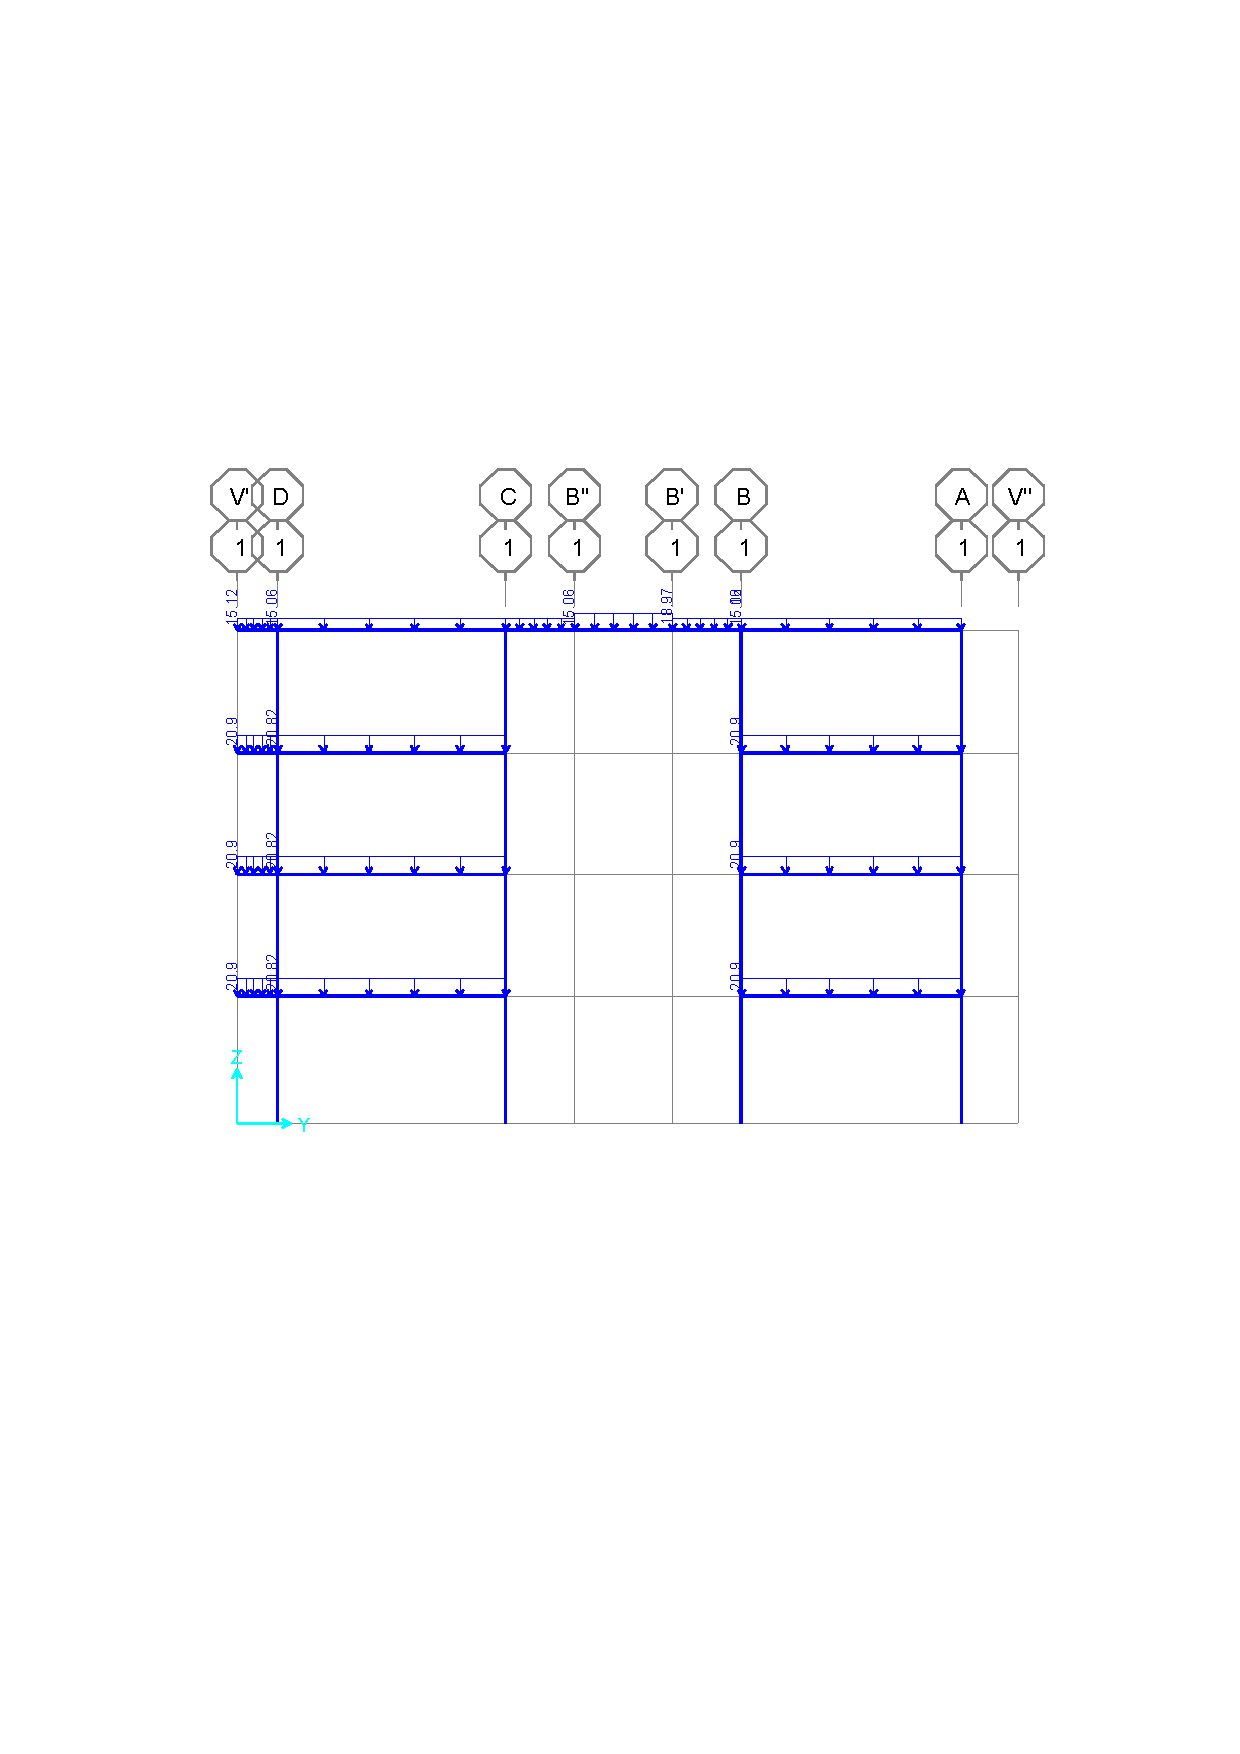
\includegraphics[scale=0.75]{images/CM 2.0/V1.pdf}
    \caption{Esquema de carga muerta viga en el eje 1}
    \label{fig:EsqVigaEje1}
\end{figure}

\begin{figure}[H]
    \centering
    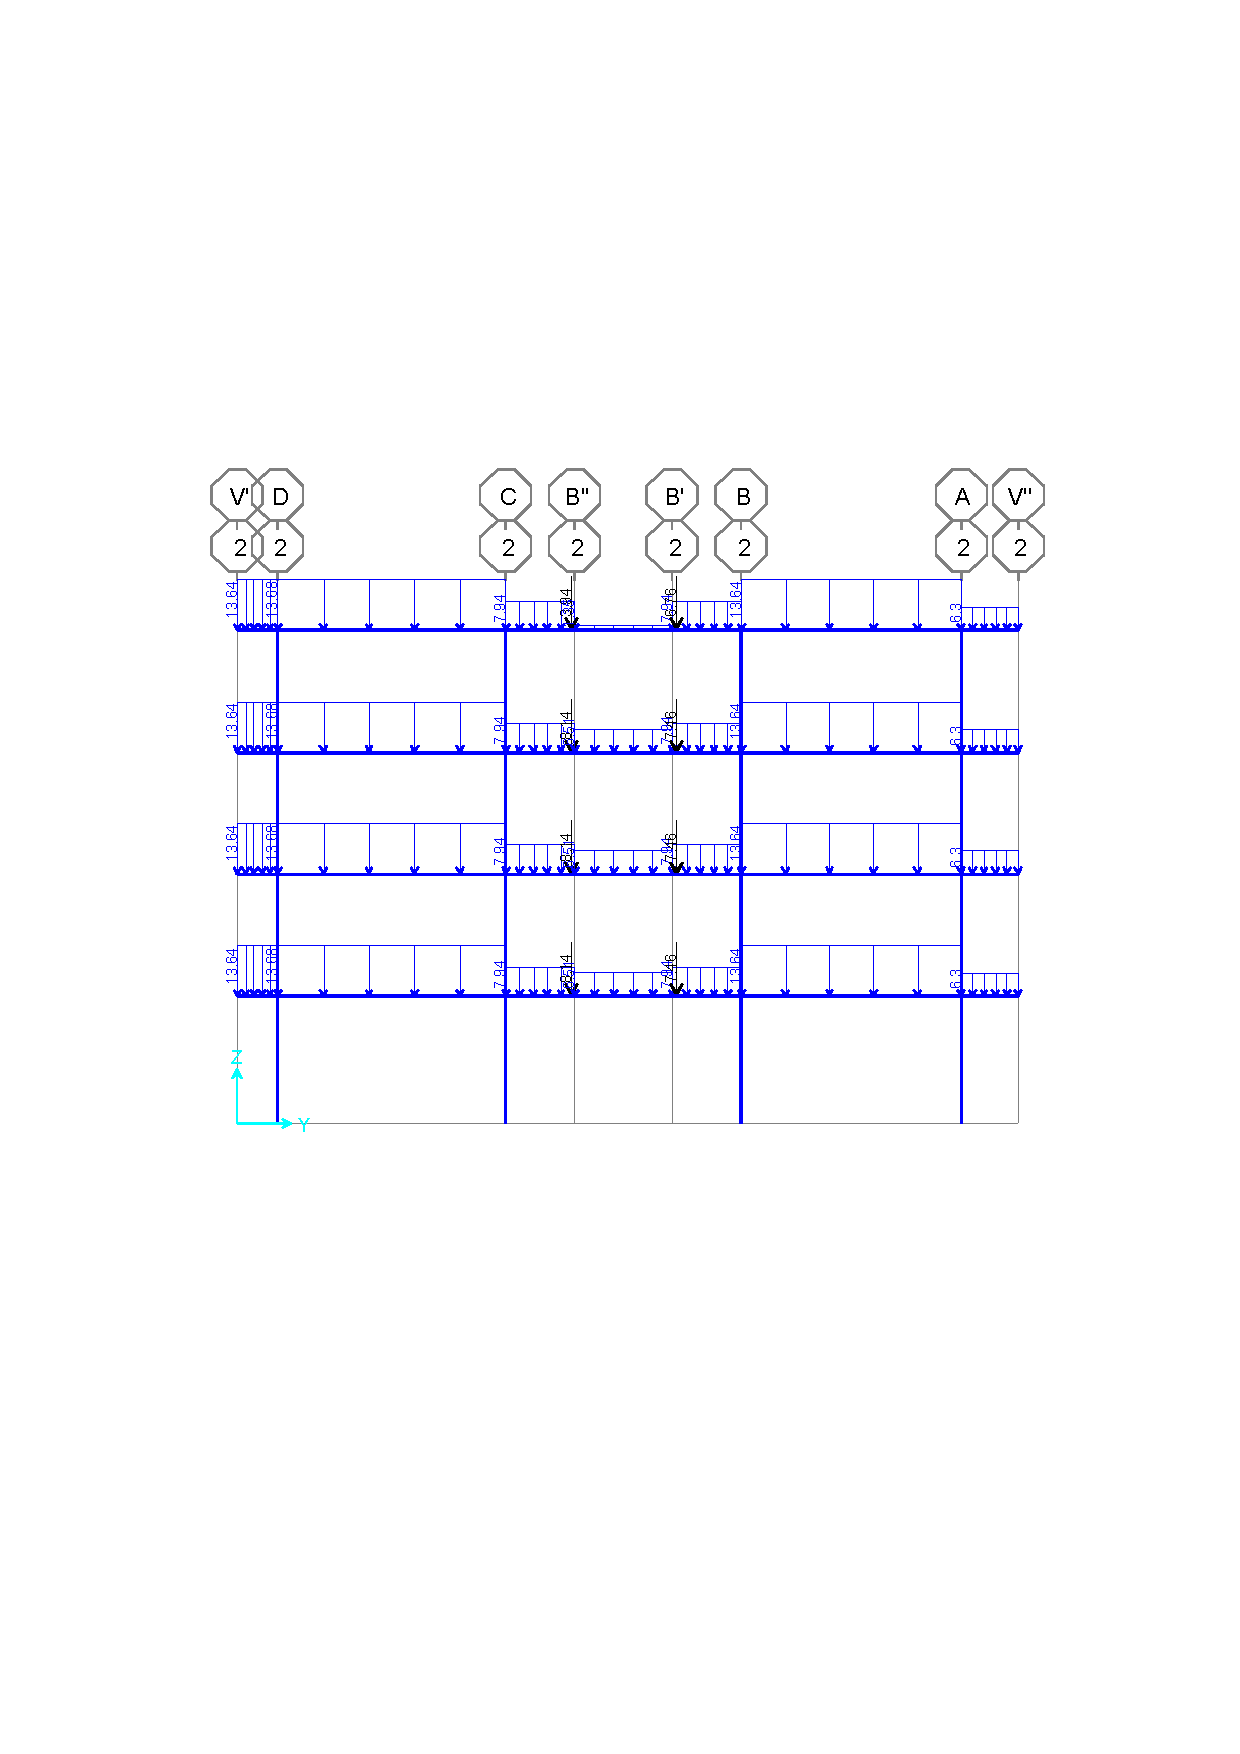
\includegraphics[scale=0.75]{images/CM 2.0/V2.pdf}
    \caption{Esquema de carga muerta viga en el eje 2}
    \label{fig:EsqVigaEje2}
\end{figure}

\begin{figure}[H]
    \centering
    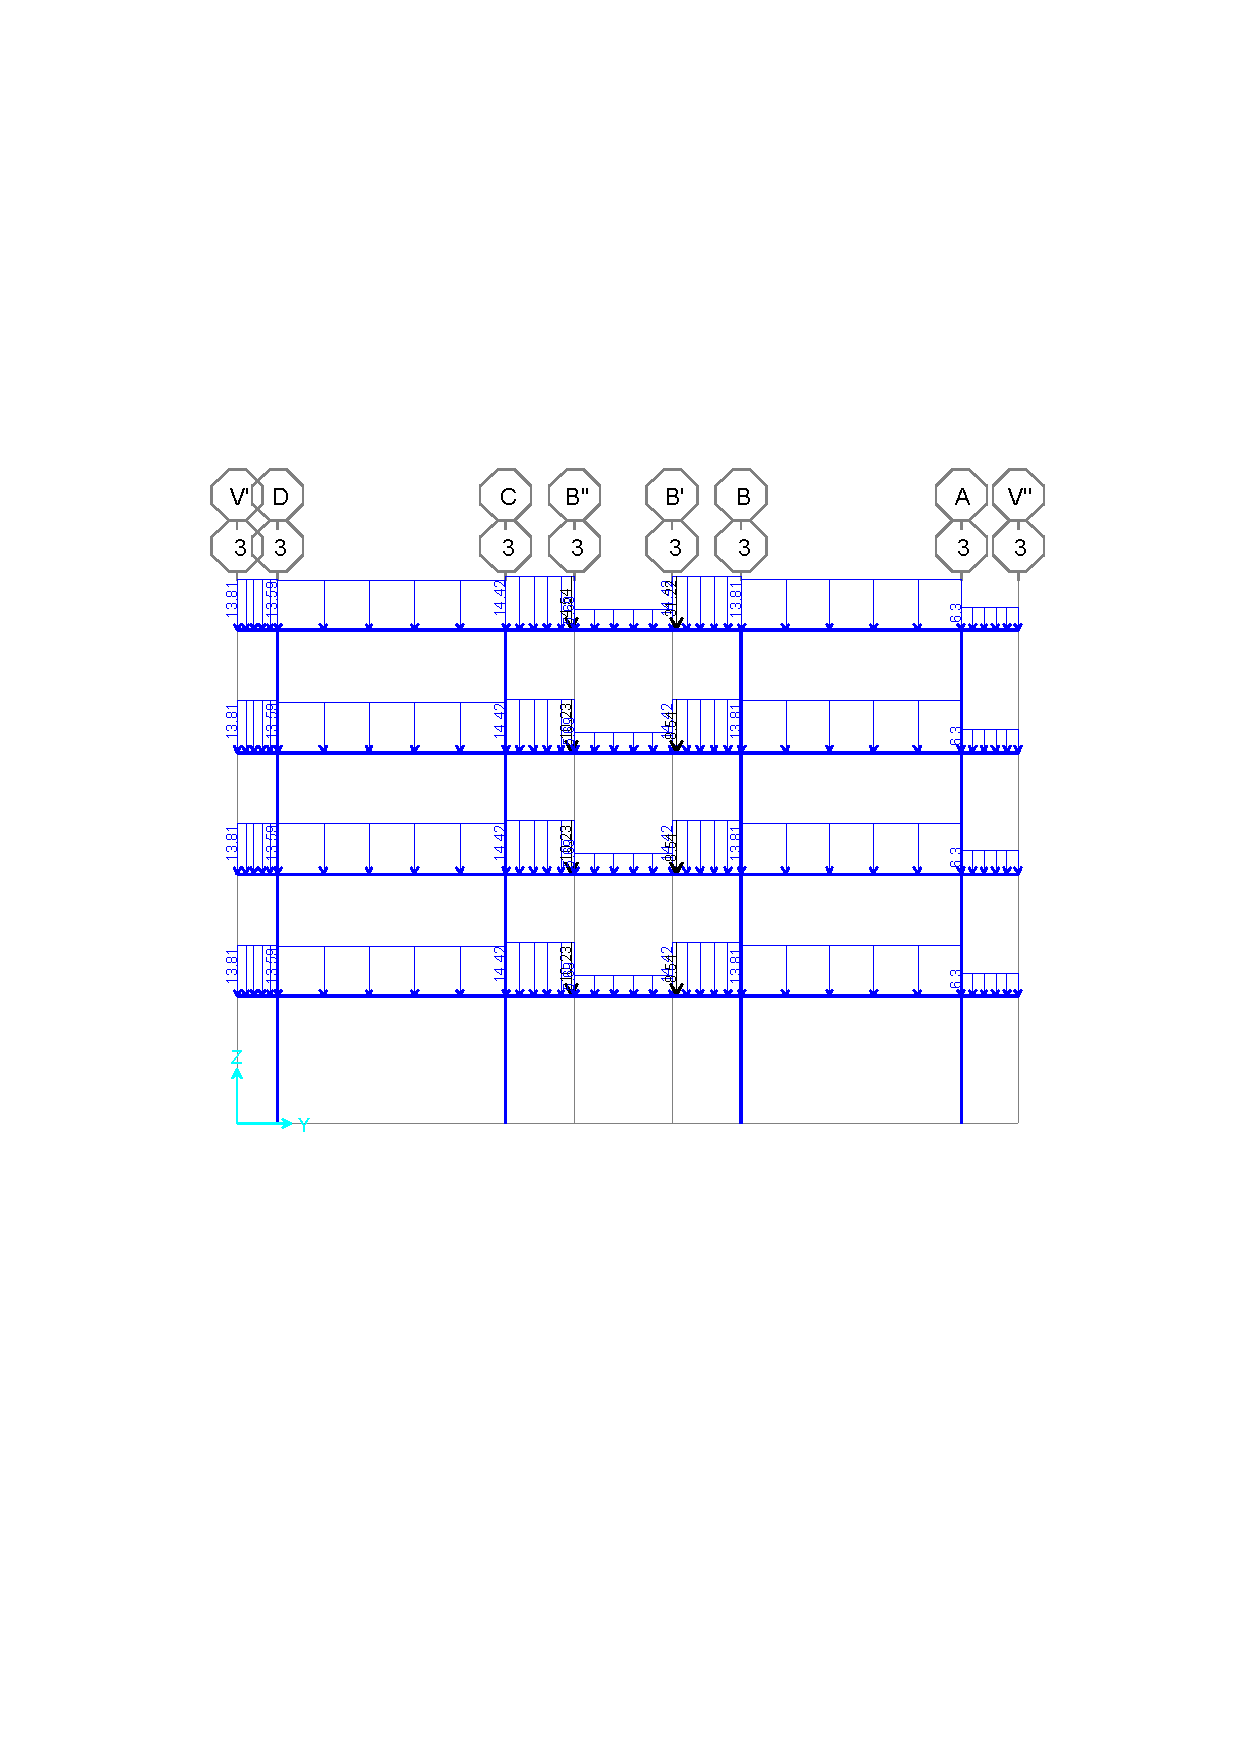
\includegraphics[scale=0.75]{images/CM 2.0/V3.pdf}
    \caption{Esquema de carga muerta viga en el eje 3}
    \label{fig:EsqVigaEje3}
\end{figure}

\begin{figure}[H]
    \centering
    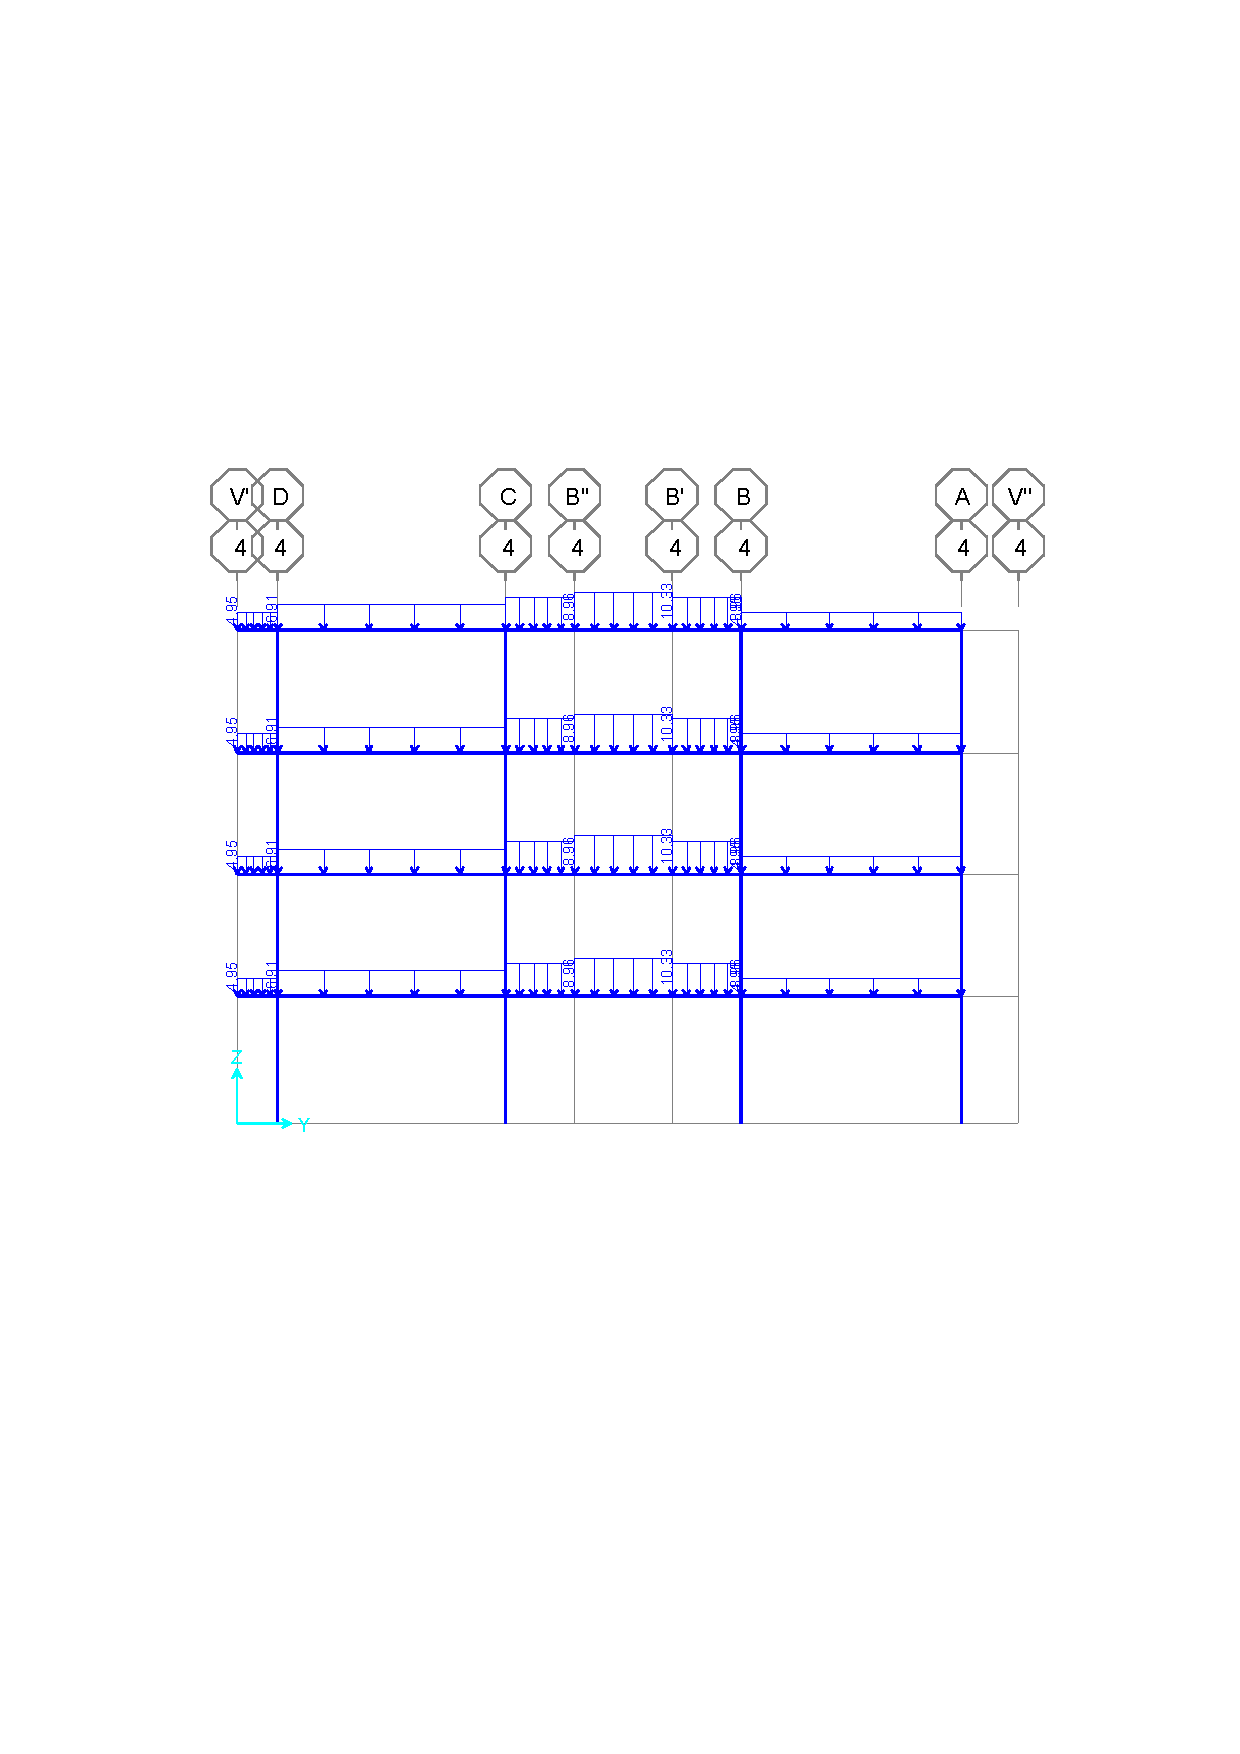
\includegraphics[scale=0.75]{images/CM 2.0/V4.pdf}
    \caption{Esquema de carga muerta viga en el eje 4}
    \label{fig:EsqVigaEje4}
\end{figure}

\begin{figure}[H]
    \centering
    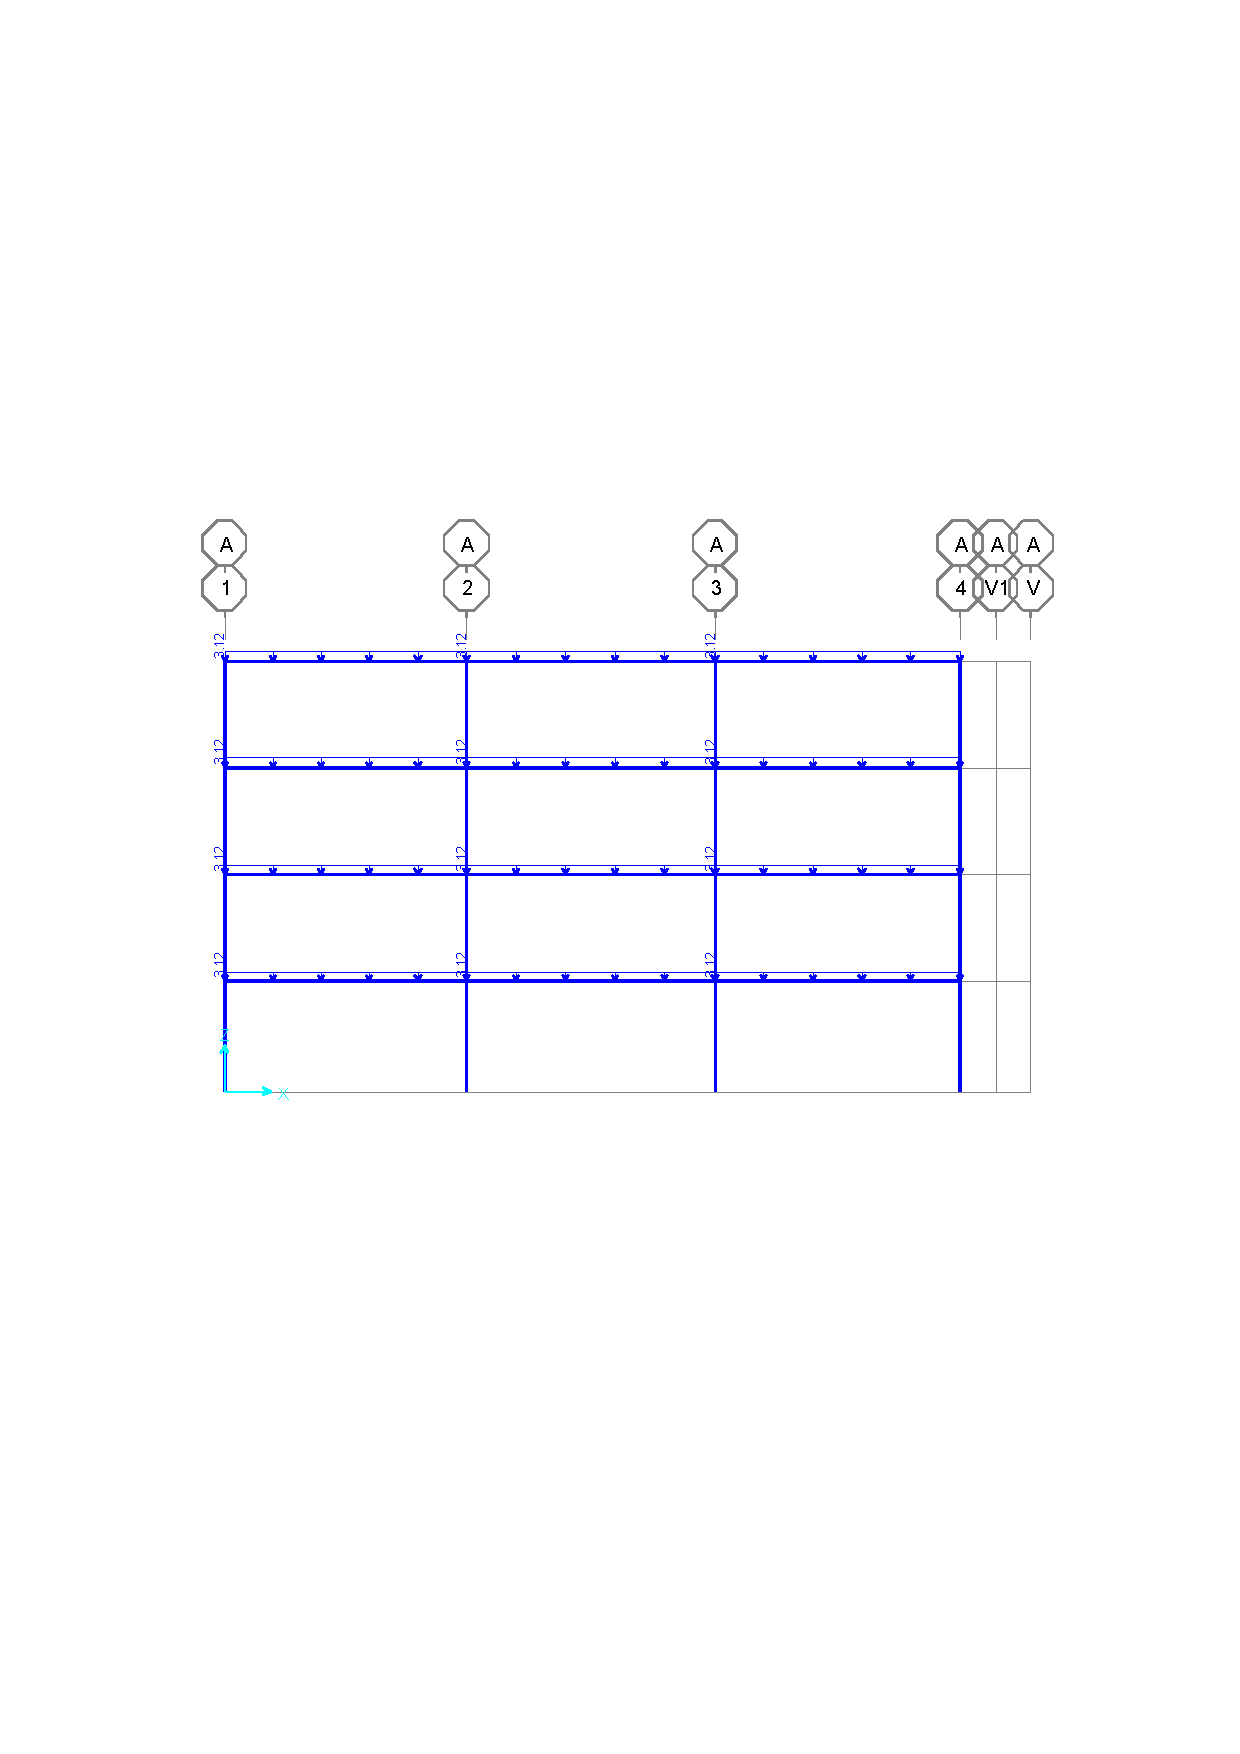
\includegraphics[scale=0.75]{images/CM 2.0/VA.pdf}
    \caption{Esquema de carga muerta viga en el eje A}
    \label{fig:EsqVigaEjeA}
\end{figure}

\begin{figure}[H]
    \centering
    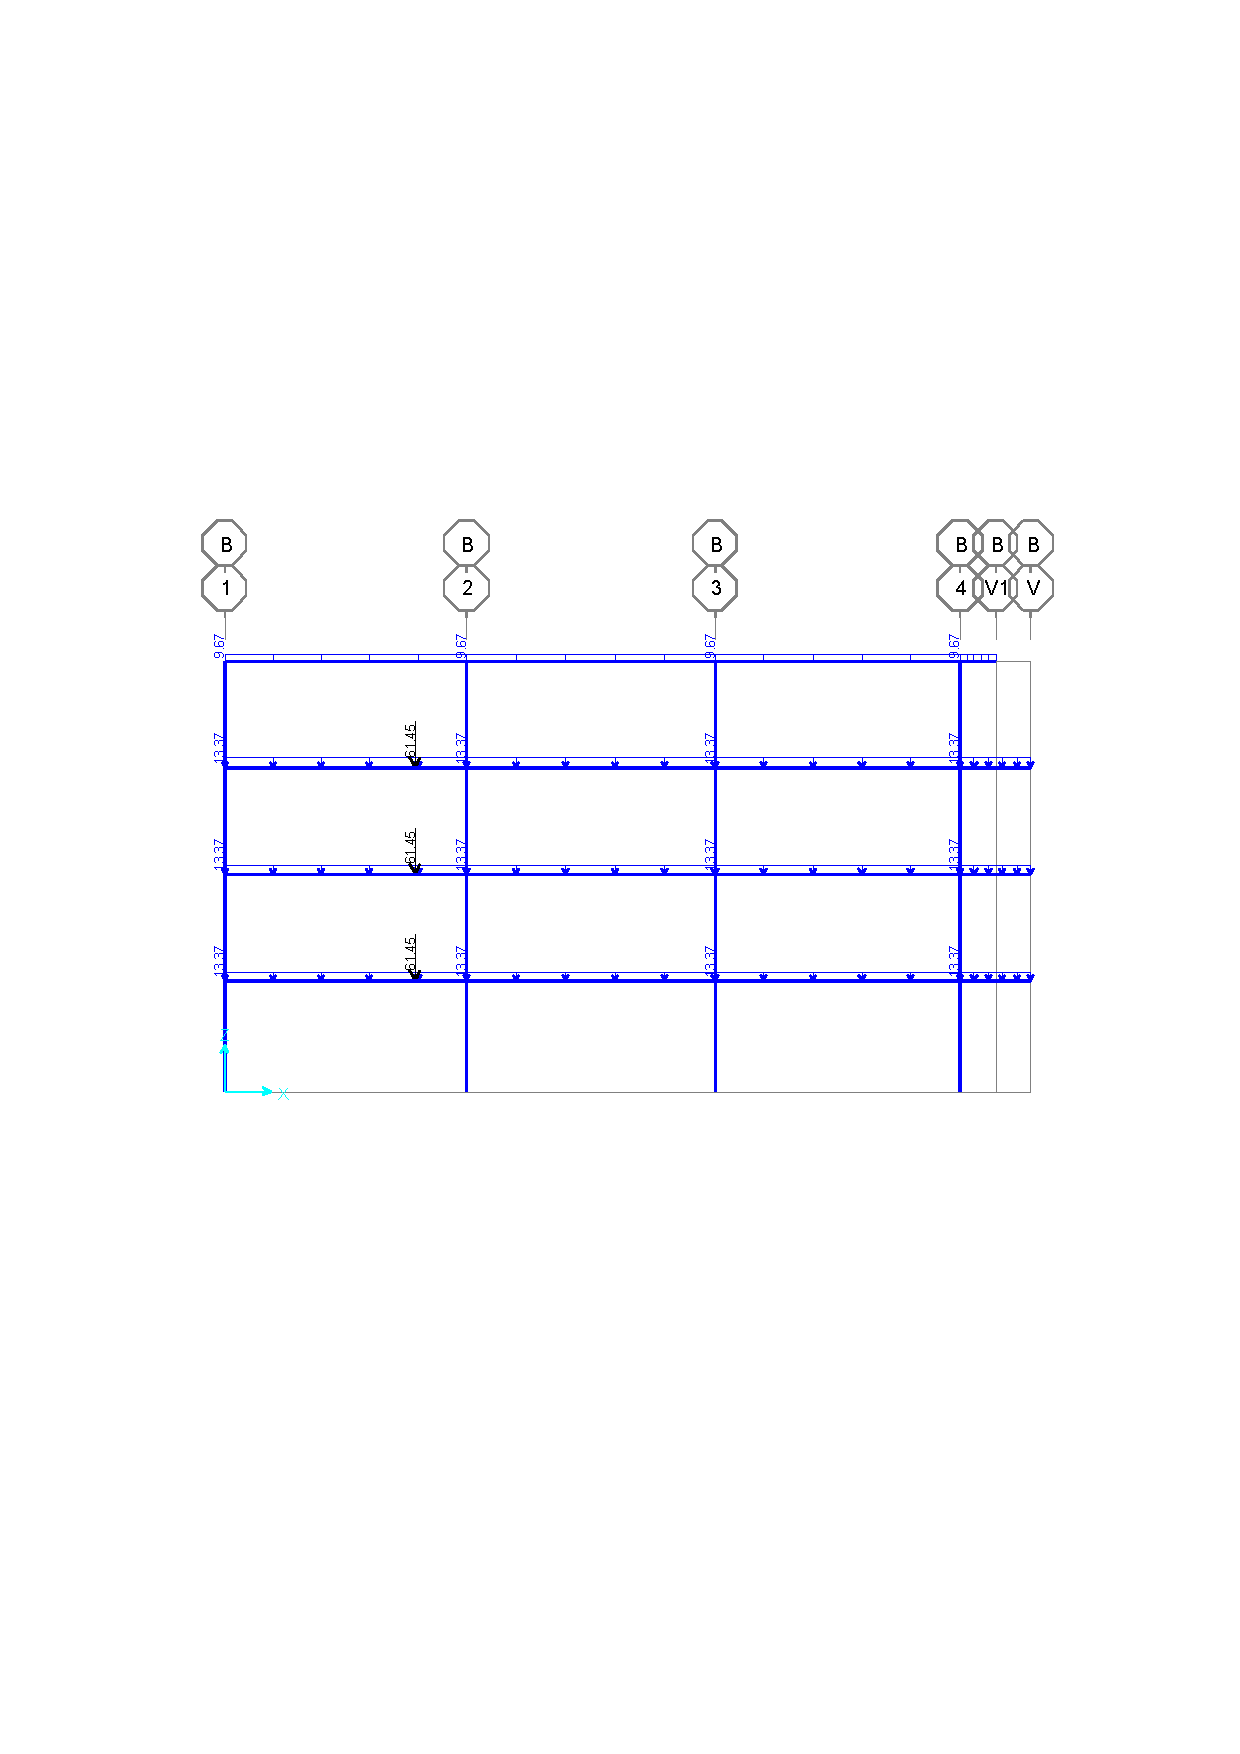
\includegraphics[scale=0.75]{images/CM 2.0/VB.pdf}
    \caption{Esquema de carga muerta viga en el eje B}
    \label{fig:EsqVigaEjeB}
\end{figure}

\begin{figure}[H]
    \centering
    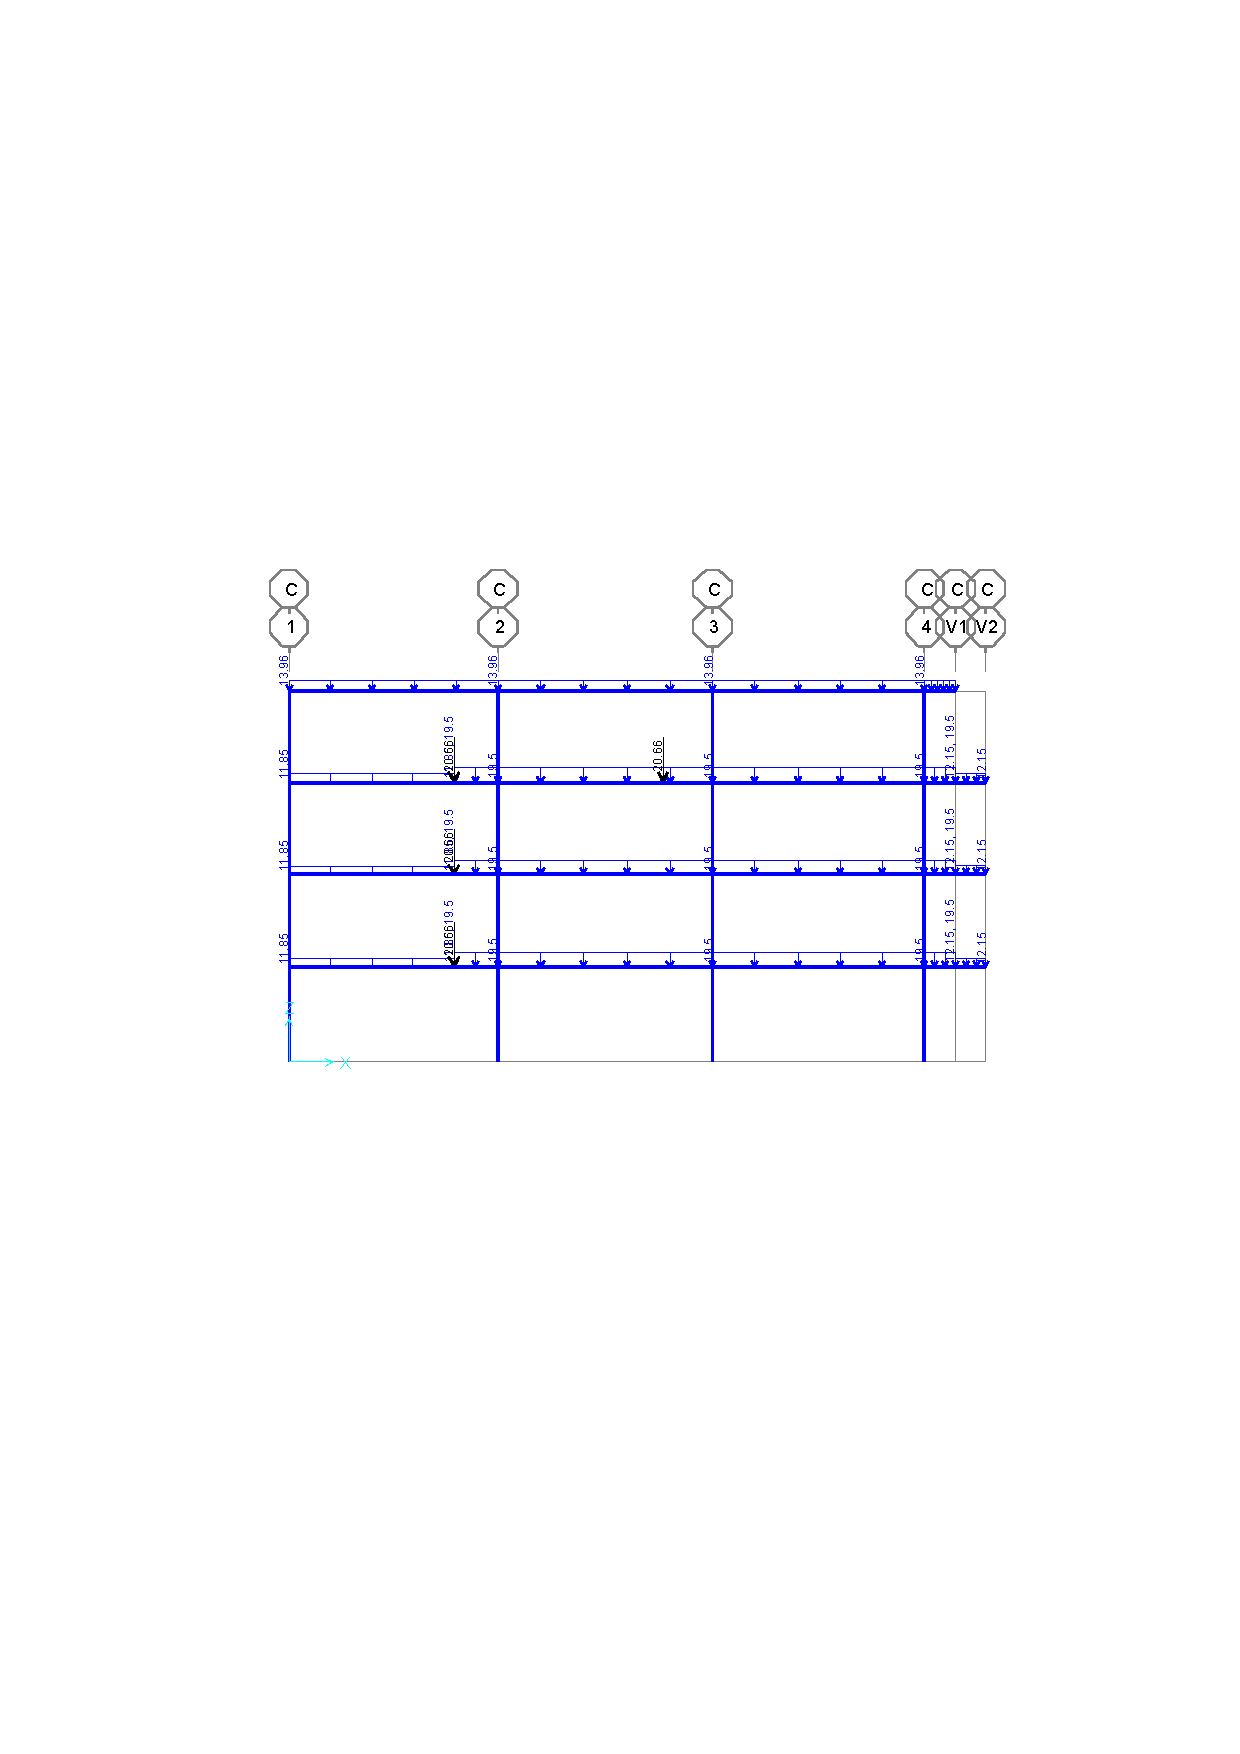
\includegraphics[scale=0.75]{images/CM 2.0/VC.pdf}
    \caption{Esquema de carga muerta viga en el eje C}
    \label{fig:EsqVigaEjeC}
\end{figure}

\begin{figure}[H]
    \centering
    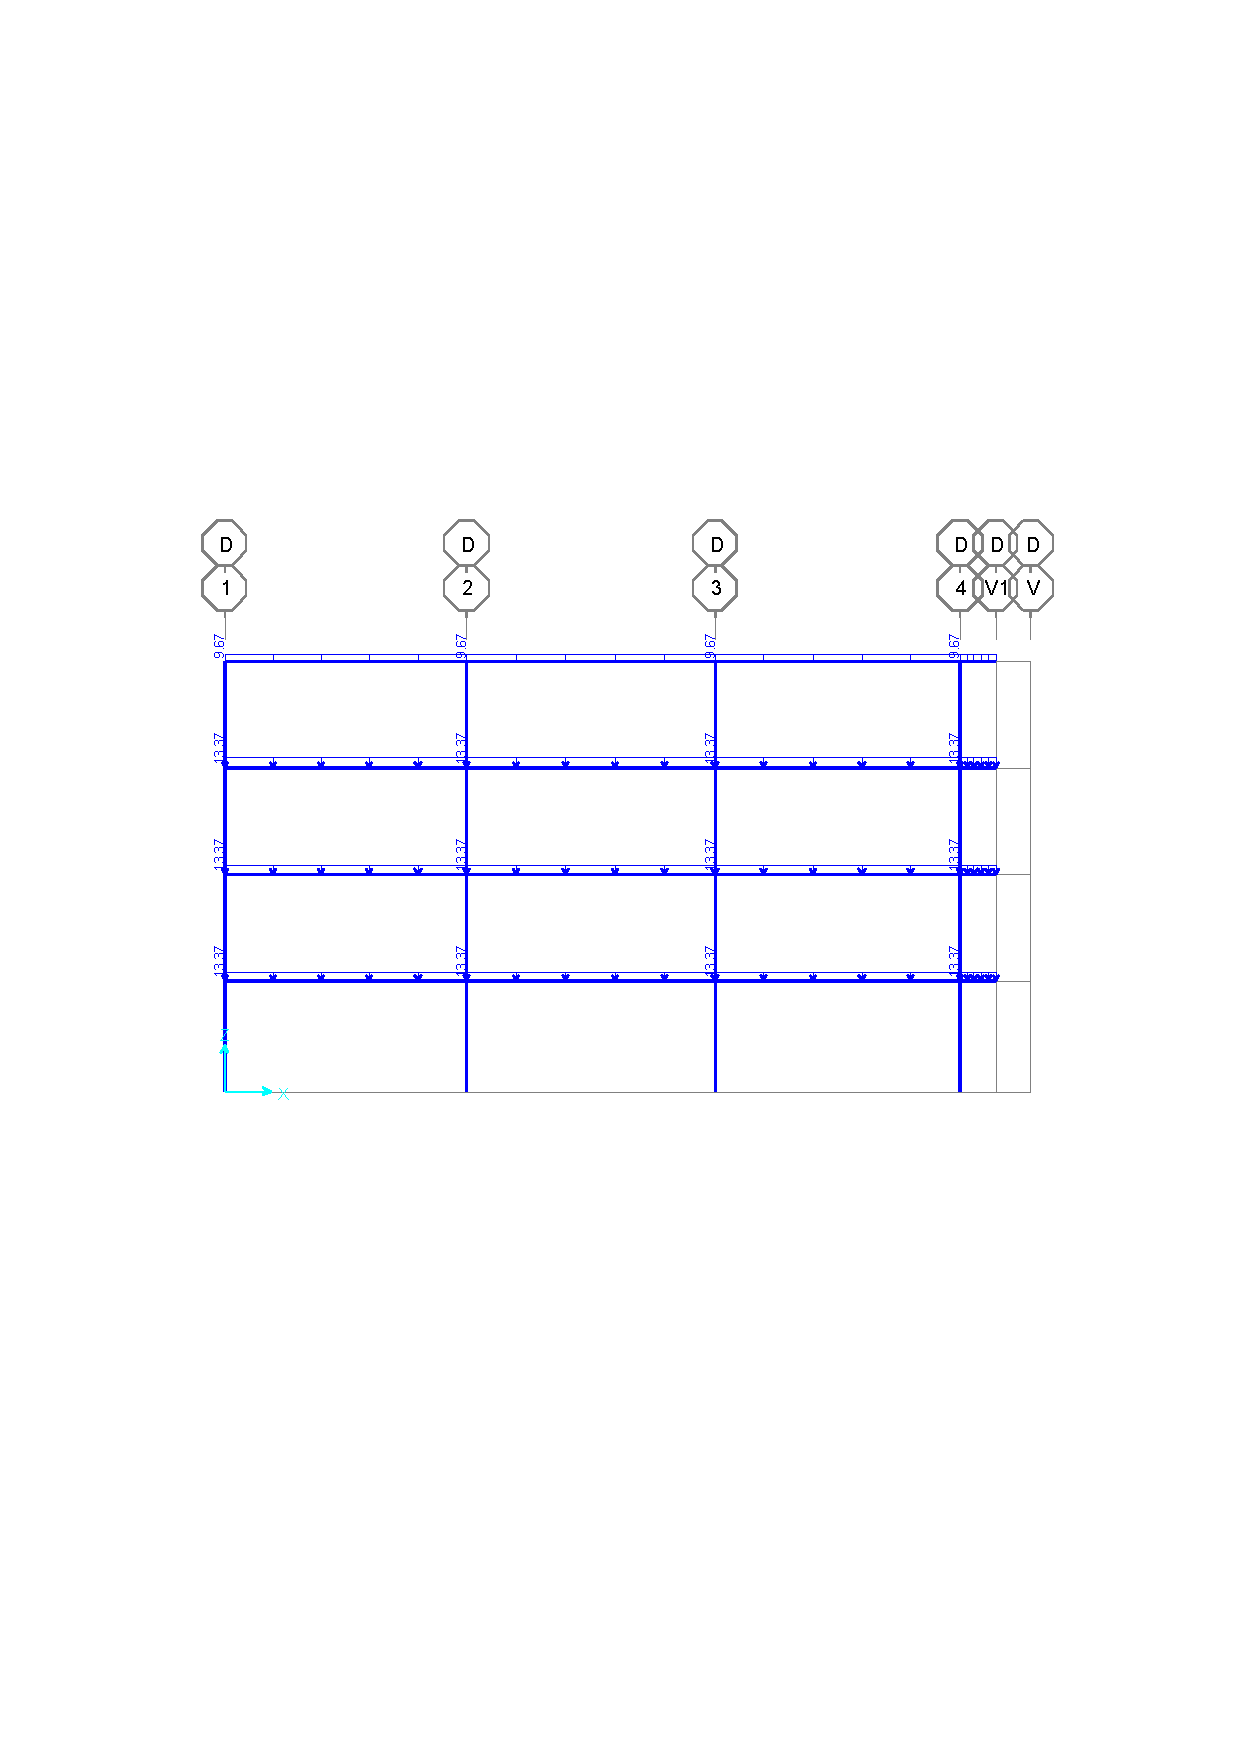
\includegraphics[scale=0.75]{images/CM 2.0/VD.pdf}
    \caption{Esquema de carga muerta viga en el eje D}
    \label{fig:EsqVigaEjeD}
\end{figure}

\subsection{Carga viva}

\begin{figure}[H]
    \centering
    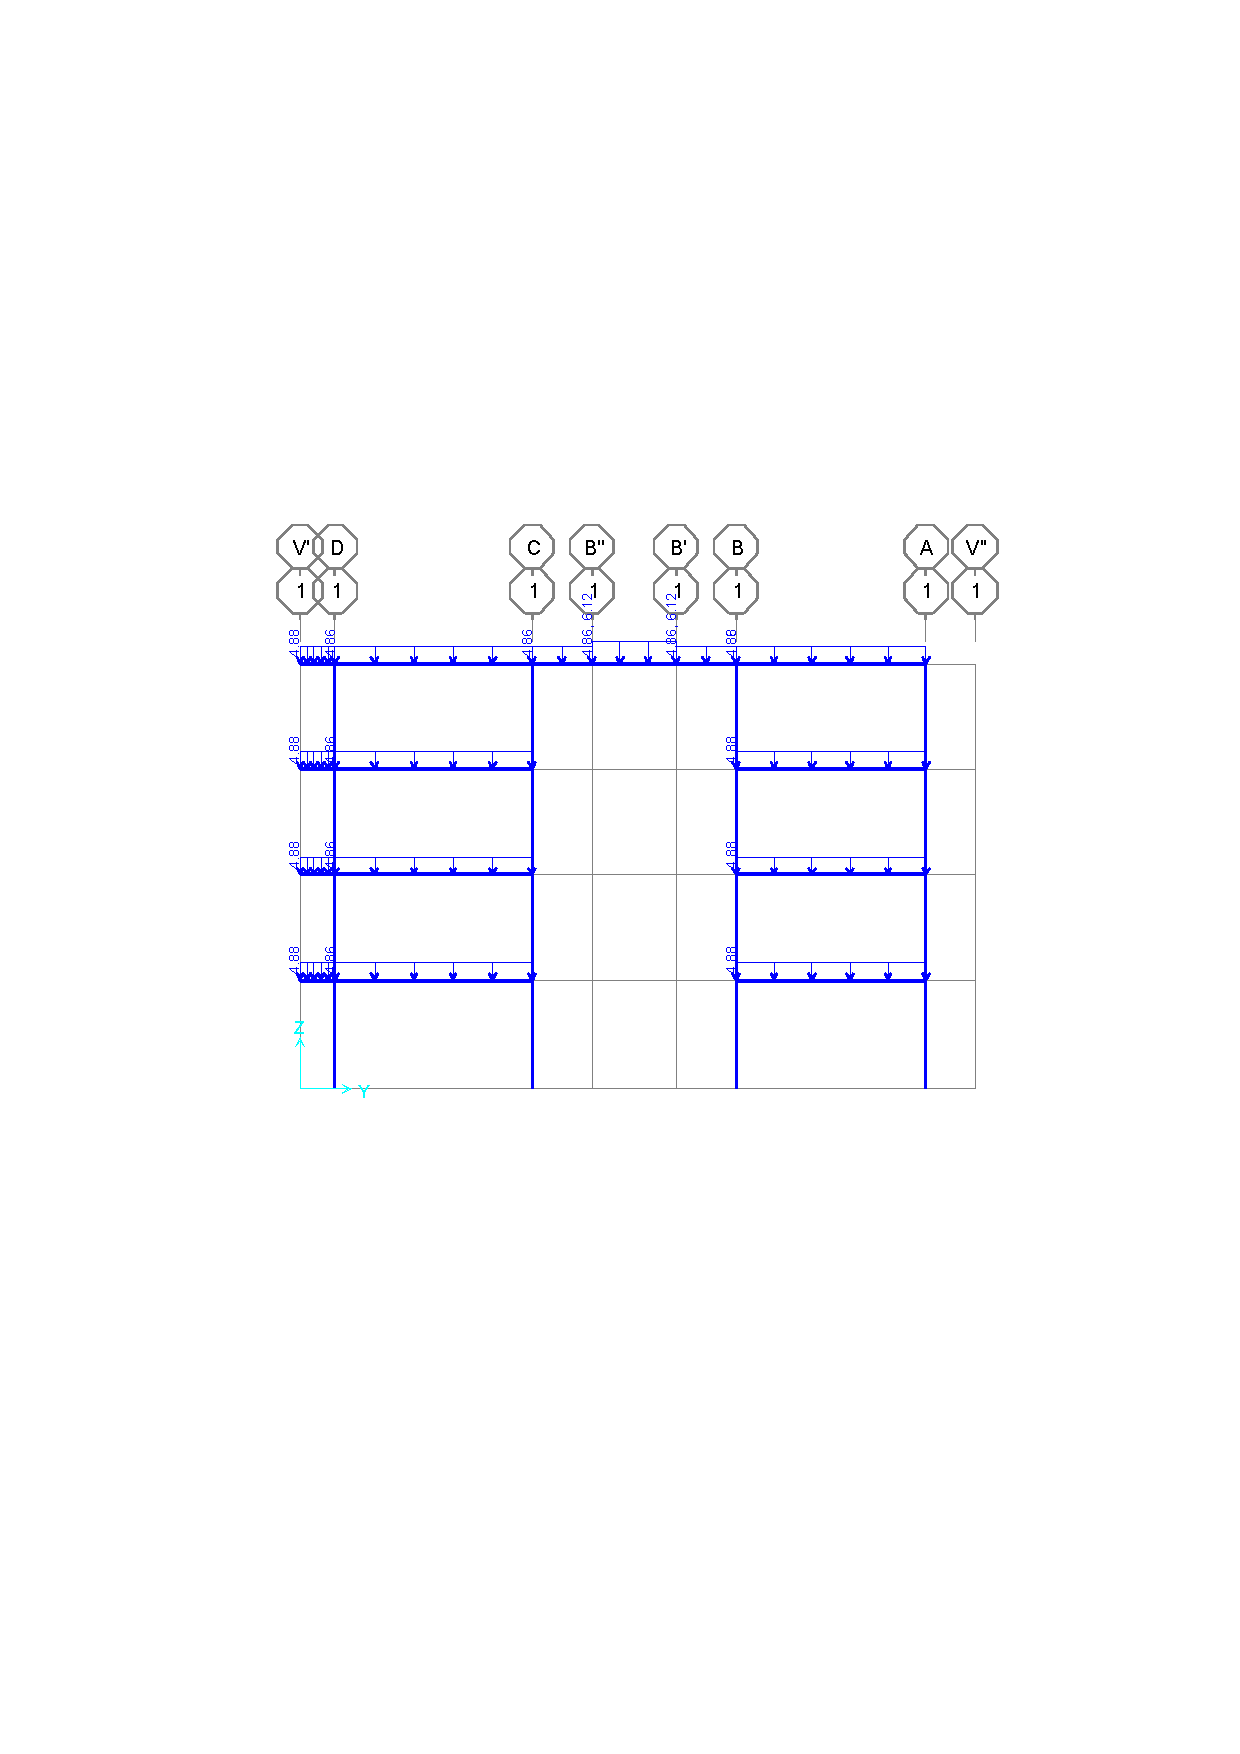
\includegraphics[scale=0.75]{images/CV 2.0/V1L.pdf}
    \caption{Esquema de carga viva viga en el eje 1}
    \label{fig:EsqVigaEje1V}
\end{figure}

\begin{figure}[H]
    \centering
    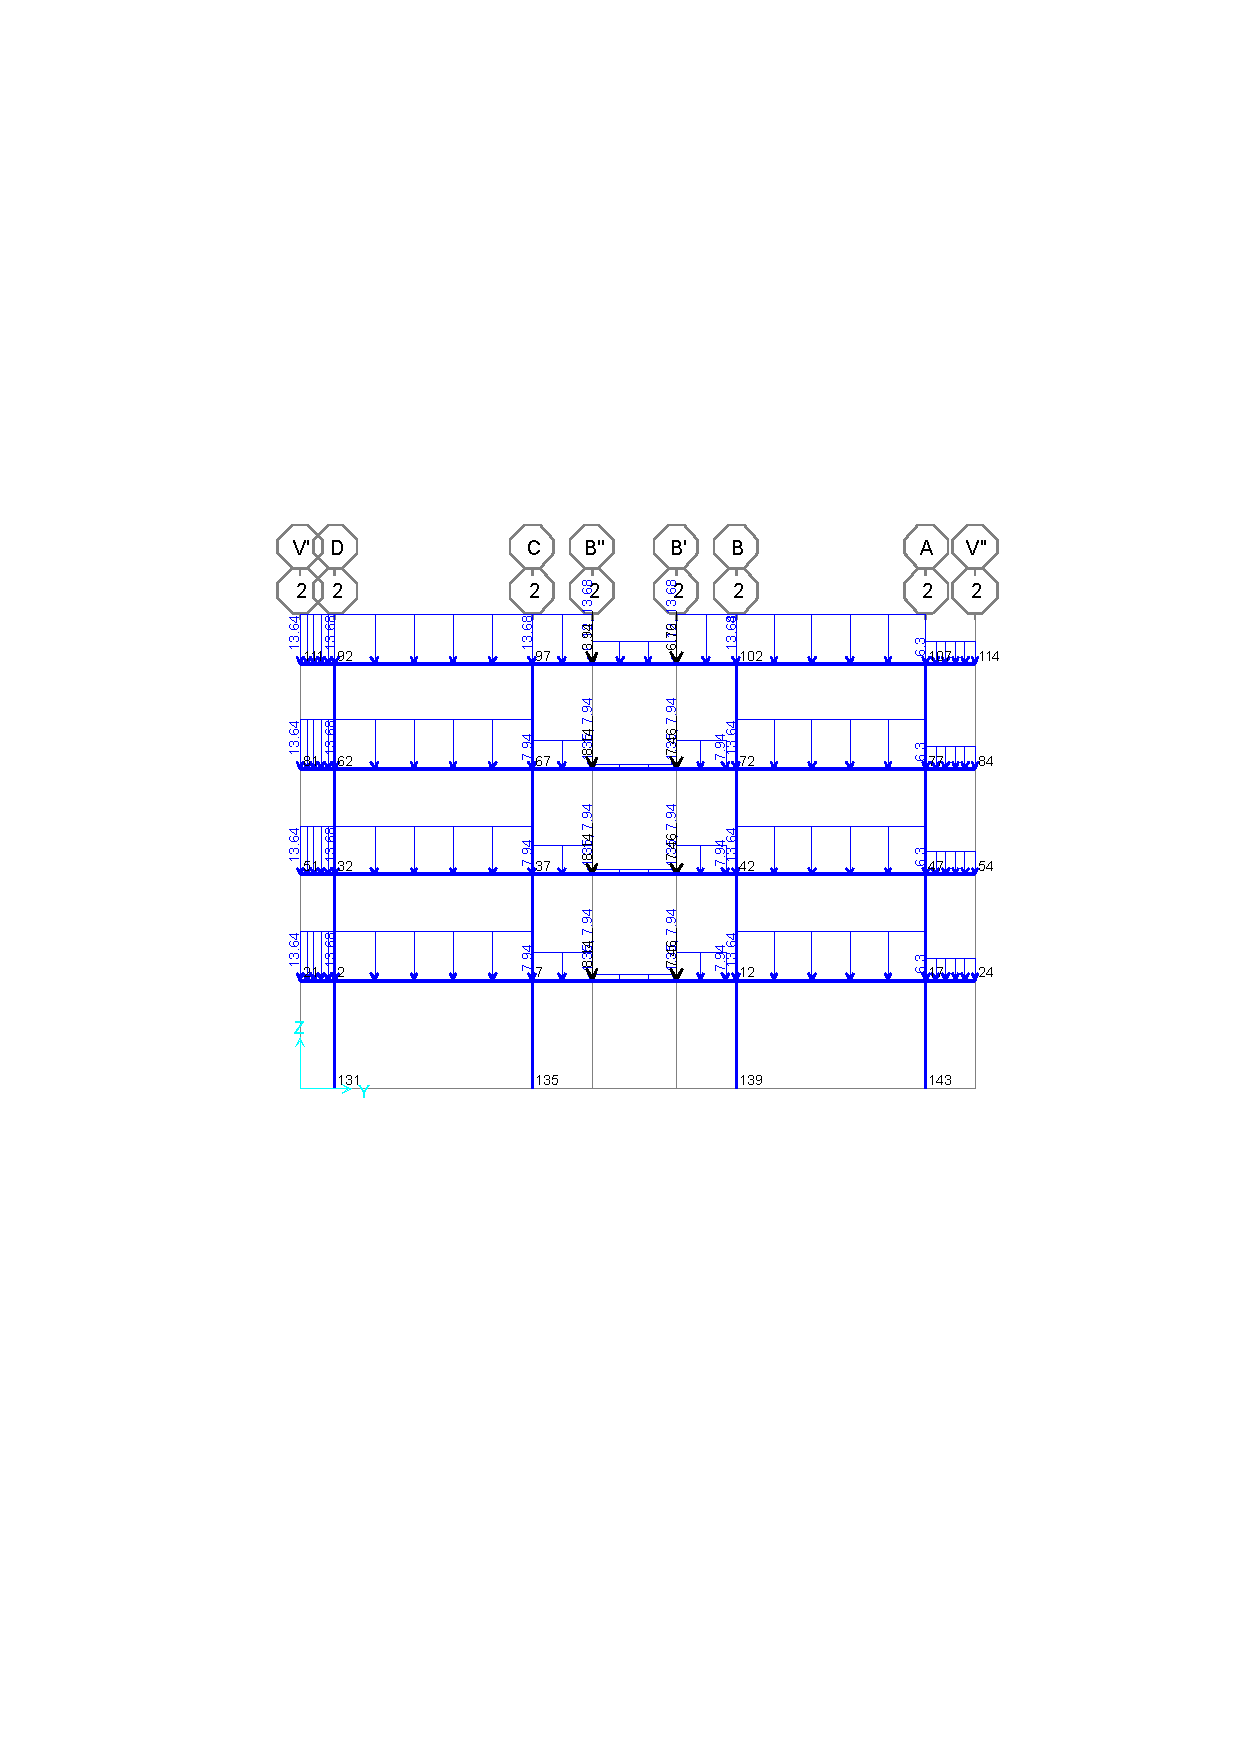
\includegraphics[scale=0.75]{images/CV 2.0/V2L.pdf}
    \caption{Esquema de carga viva viga en el eje 2}
    \label{fig:EsqVigaEje2V}
\end{figure}

\begin{figure}[H]
    \centering
    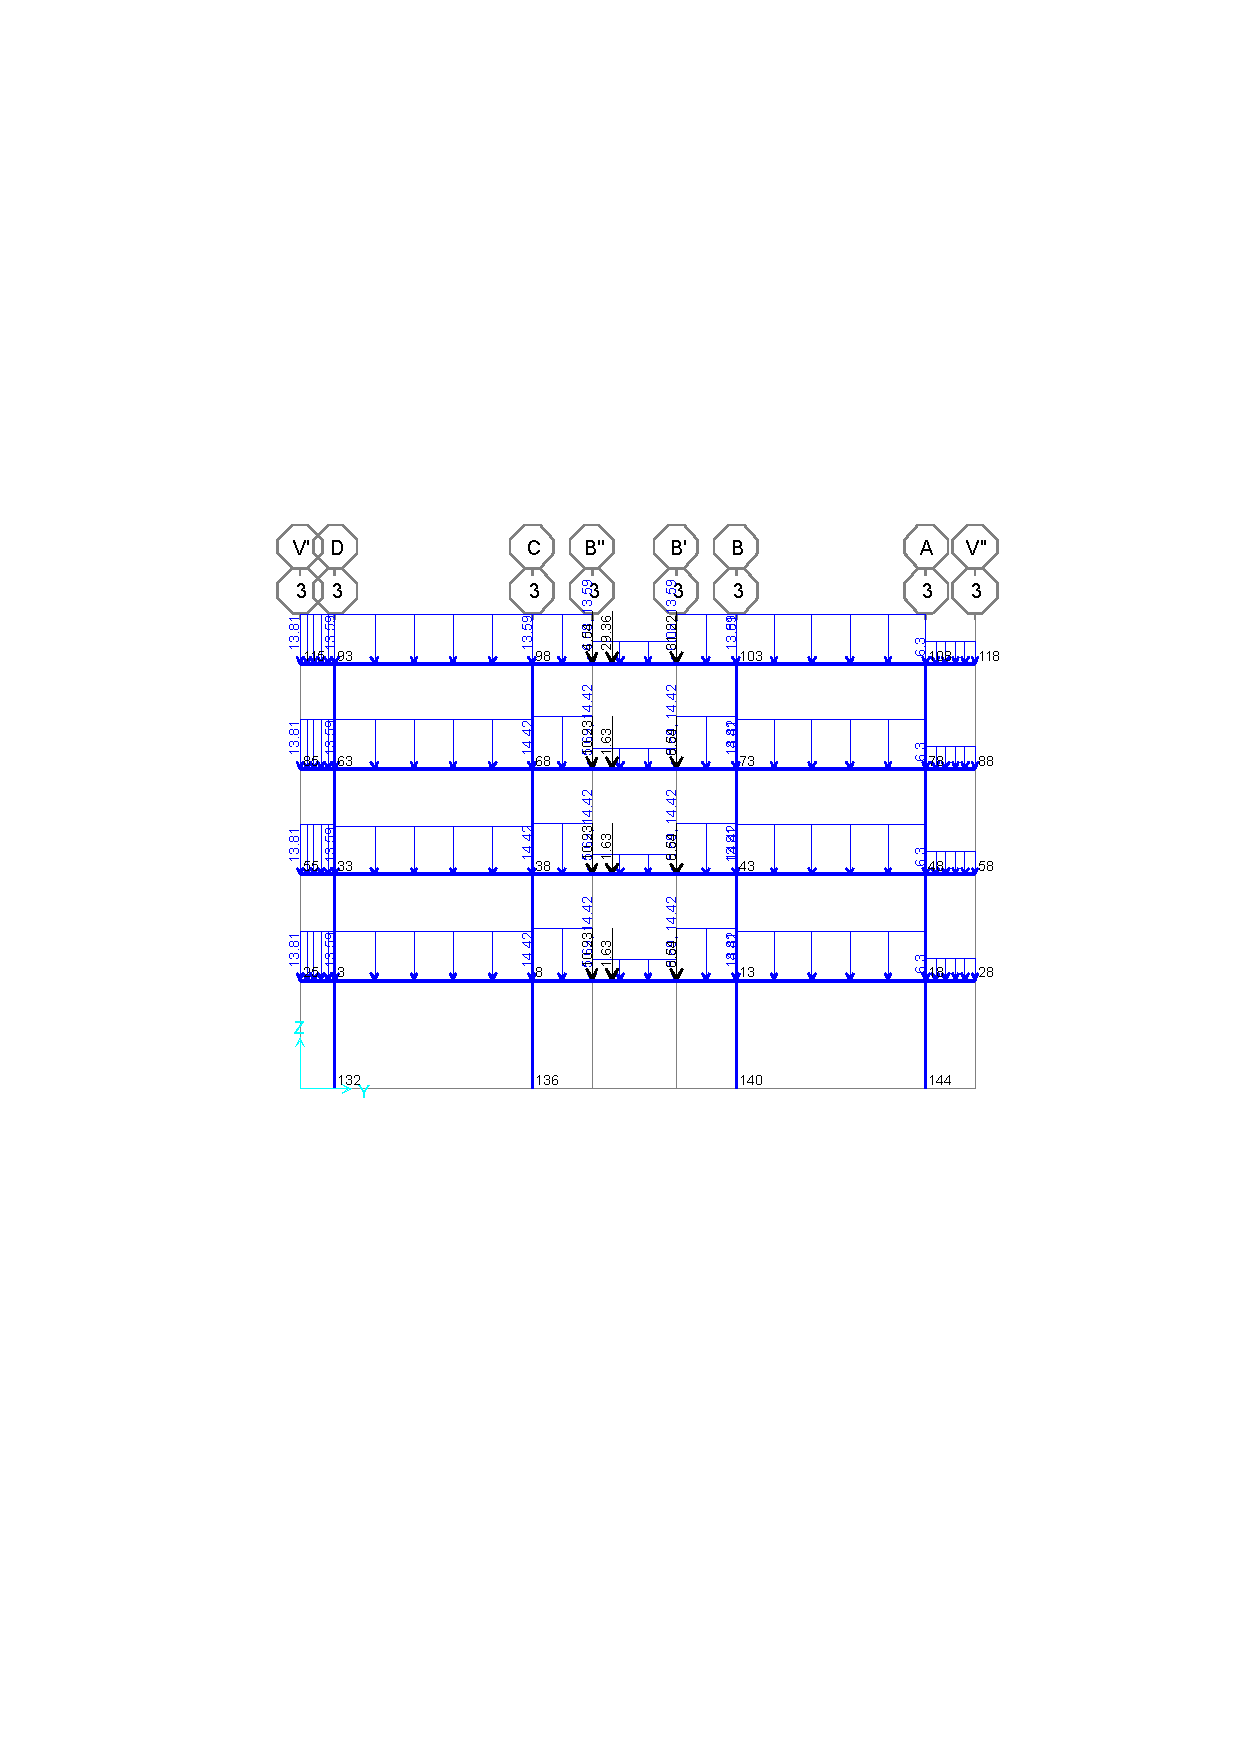
\includegraphics[scale=0.75]{images/CV 2.0/V3L.pdf}
    \caption{Esquema de carga viva viga en el eje 3}
    \label{fig:EsqVigaEje3V}
\end{figure}

\begin{figure}[H]
    \centering
    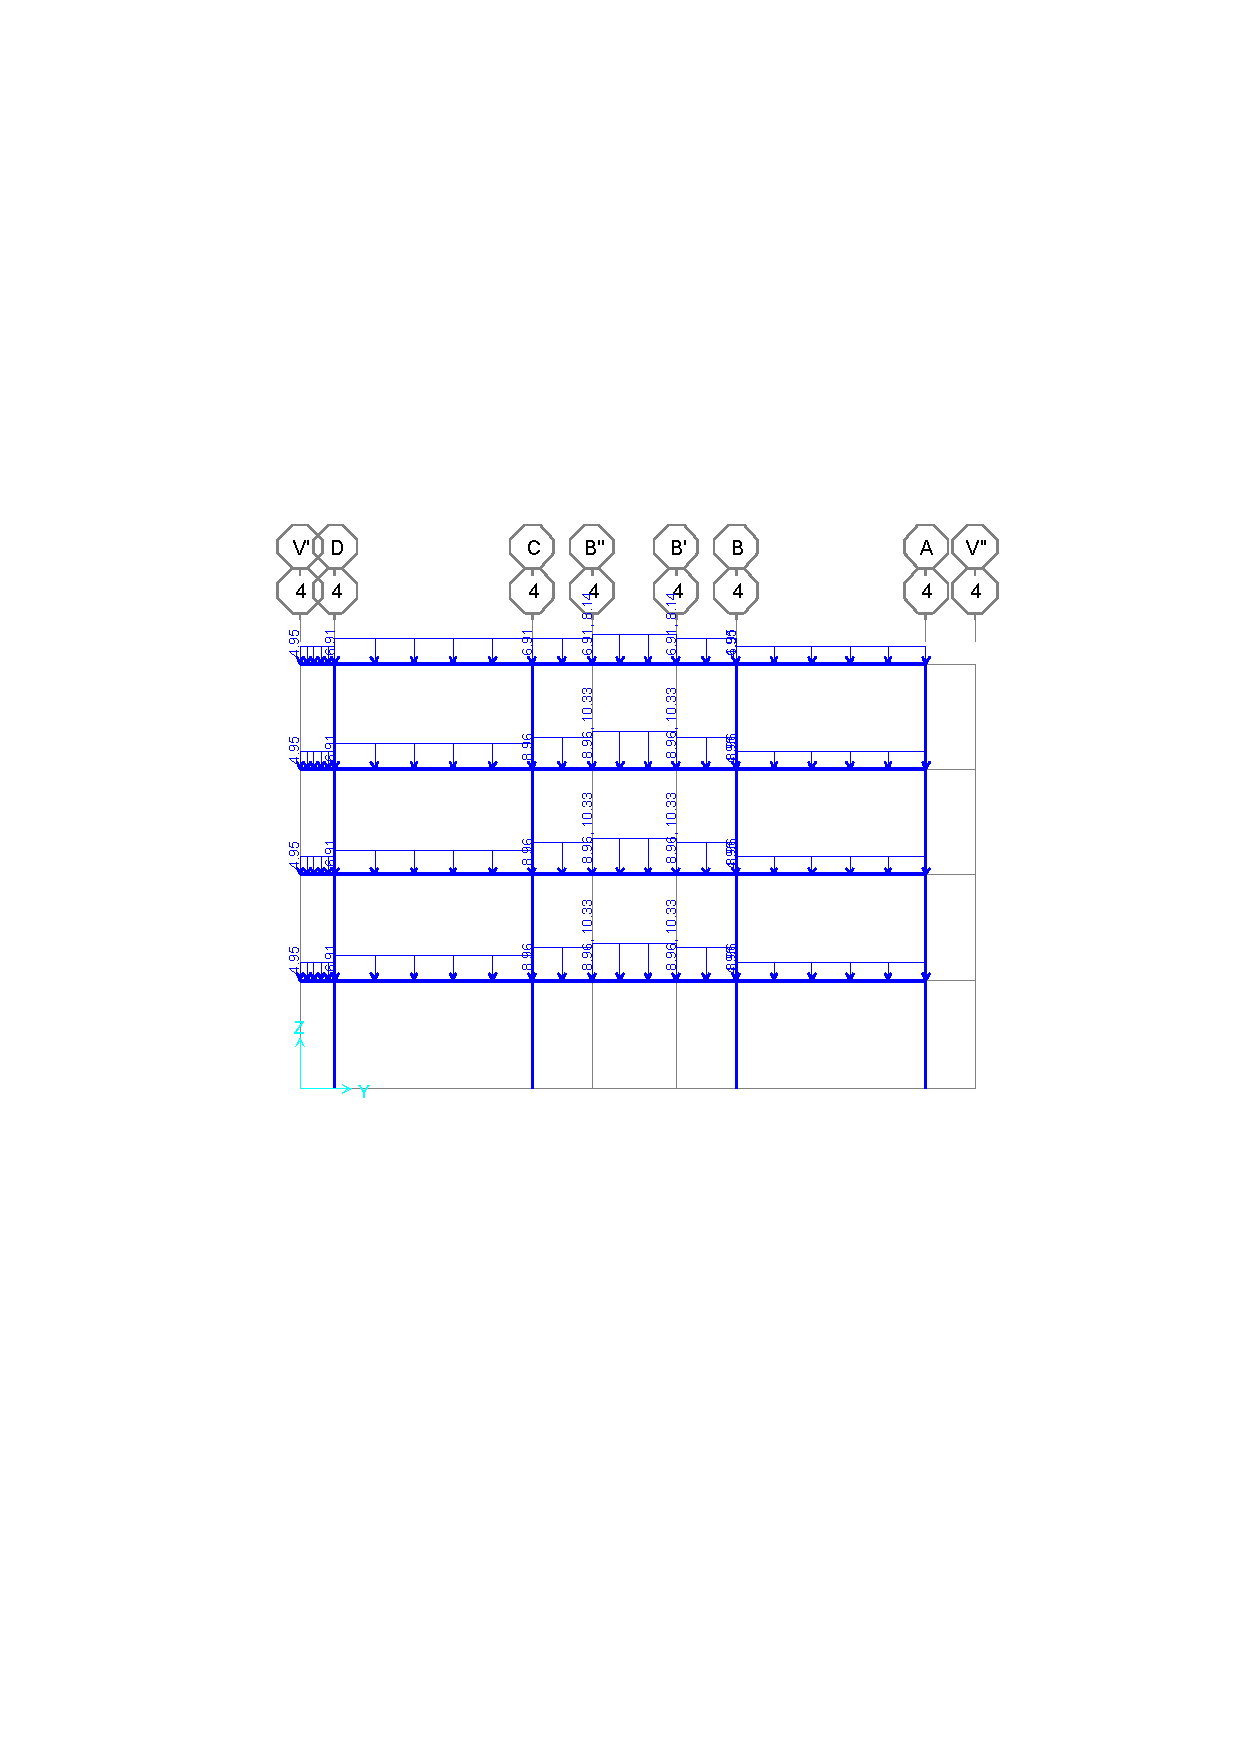
\includegraphics[scale=0.75]{images/CV 2.0/V4L.pdf}
    \caption{Esquema de carga viva viga en el eje 4}
    \label{fig:EsqVigaEje4V}
\end{figure}

\begin{figure}[H]
    \centering
    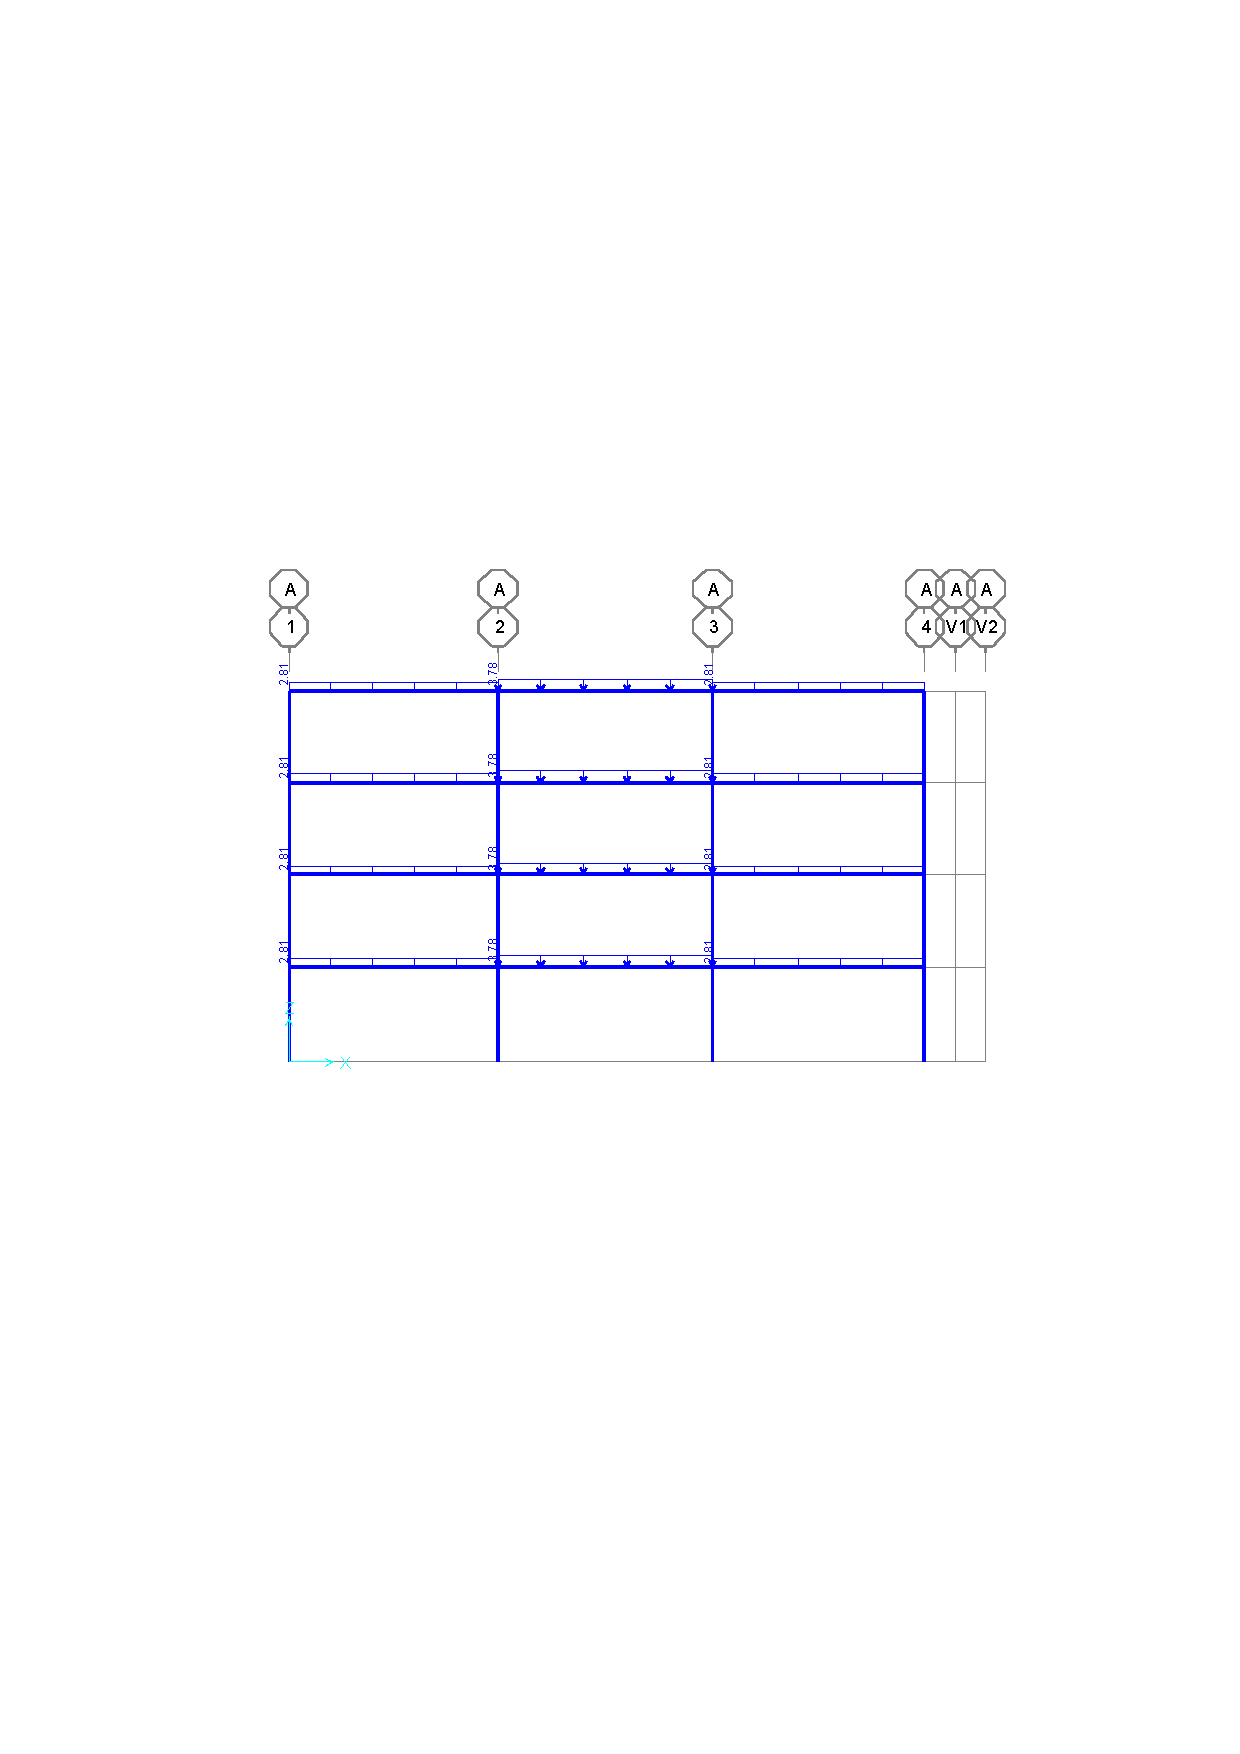
\includegraphics[scale=0.75]{images/CV 2.0/VAL.pdf}
    \caption{Esquema de carga viva viga en el eje A}
    \label{fig:EsqVigaEjeAV}
\end{figure}

\begin{figure}[H]
    \centering
    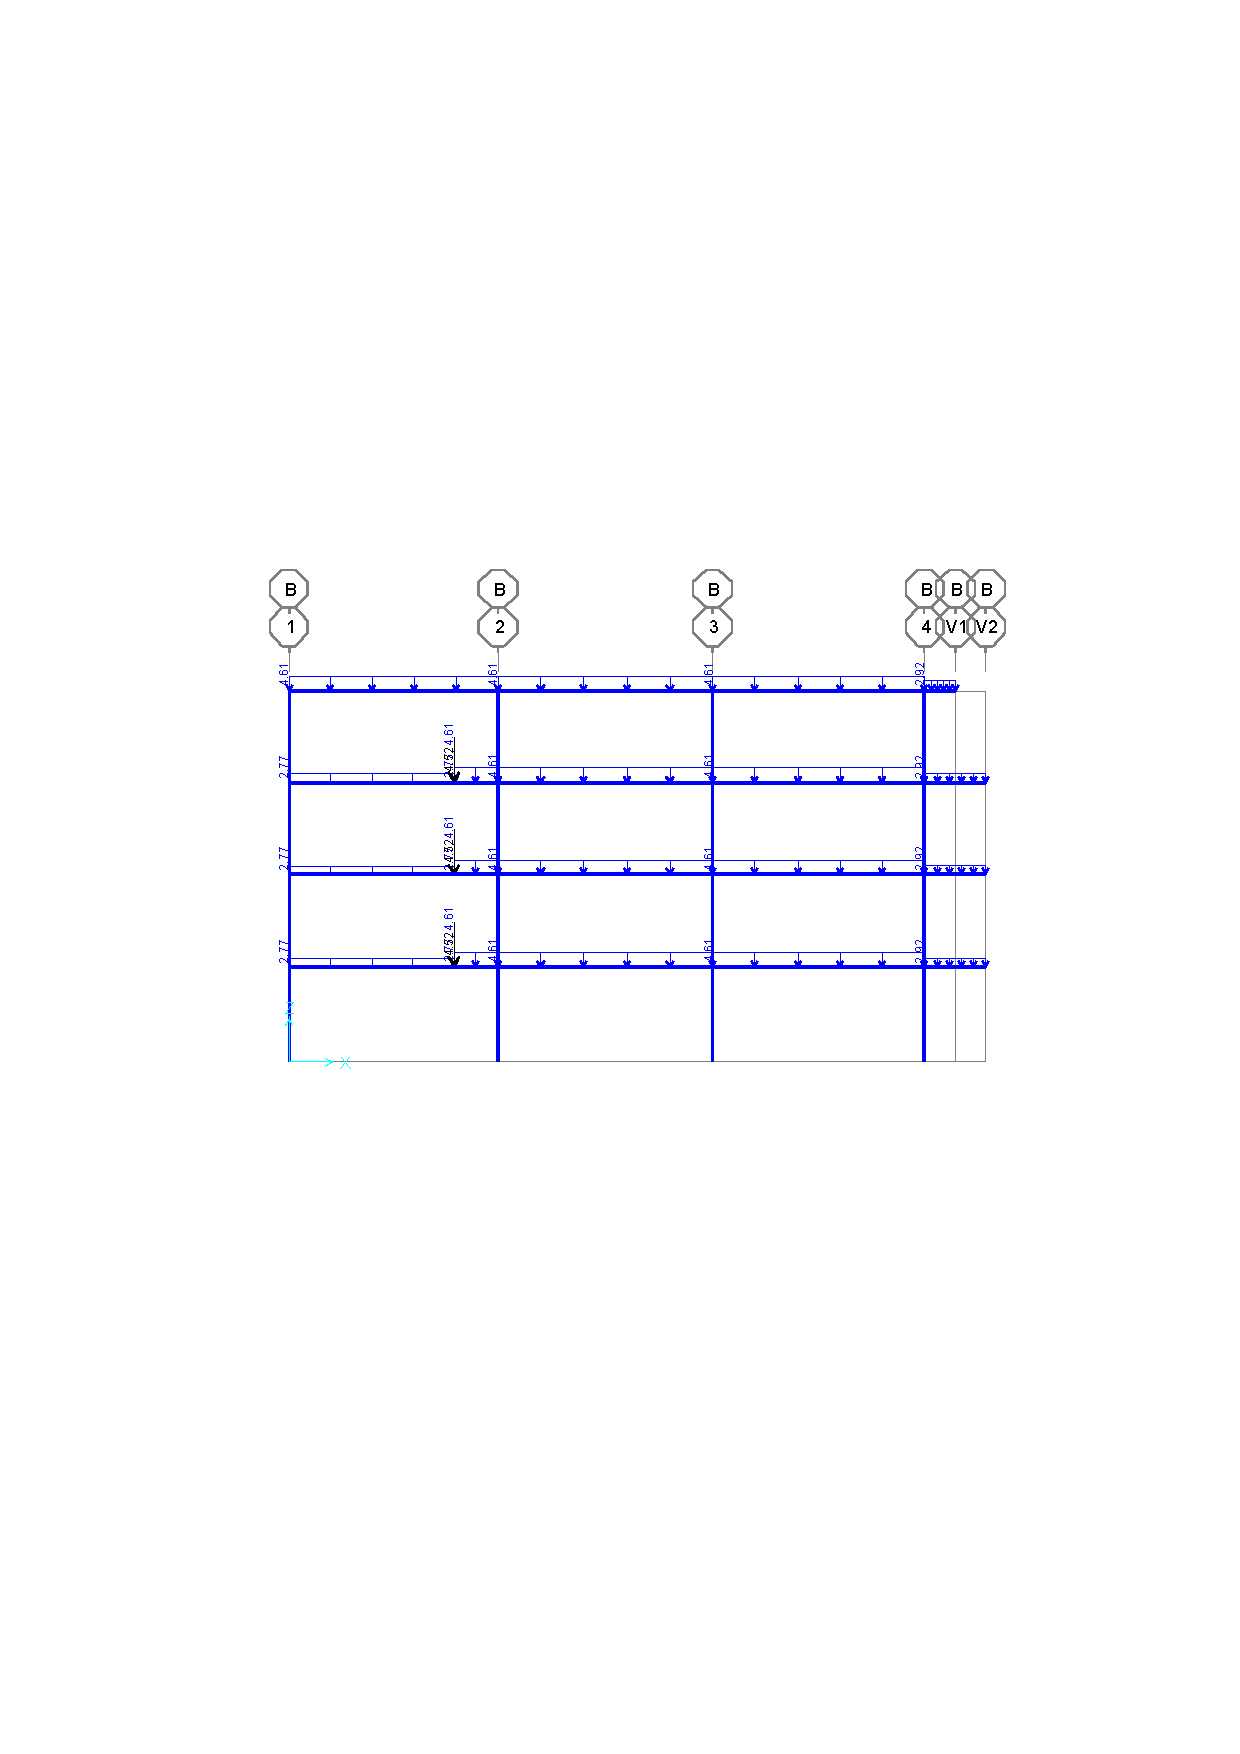
\includegraphics[scale=0.75]{images/CV 2.0/VBL.pdf}
    \caption{Esquema de carga viva viga en el eje B}
    \label{fig:EsqVigaEjeBV}
\end{figure}

\begin{figure}[H]
    \centering
    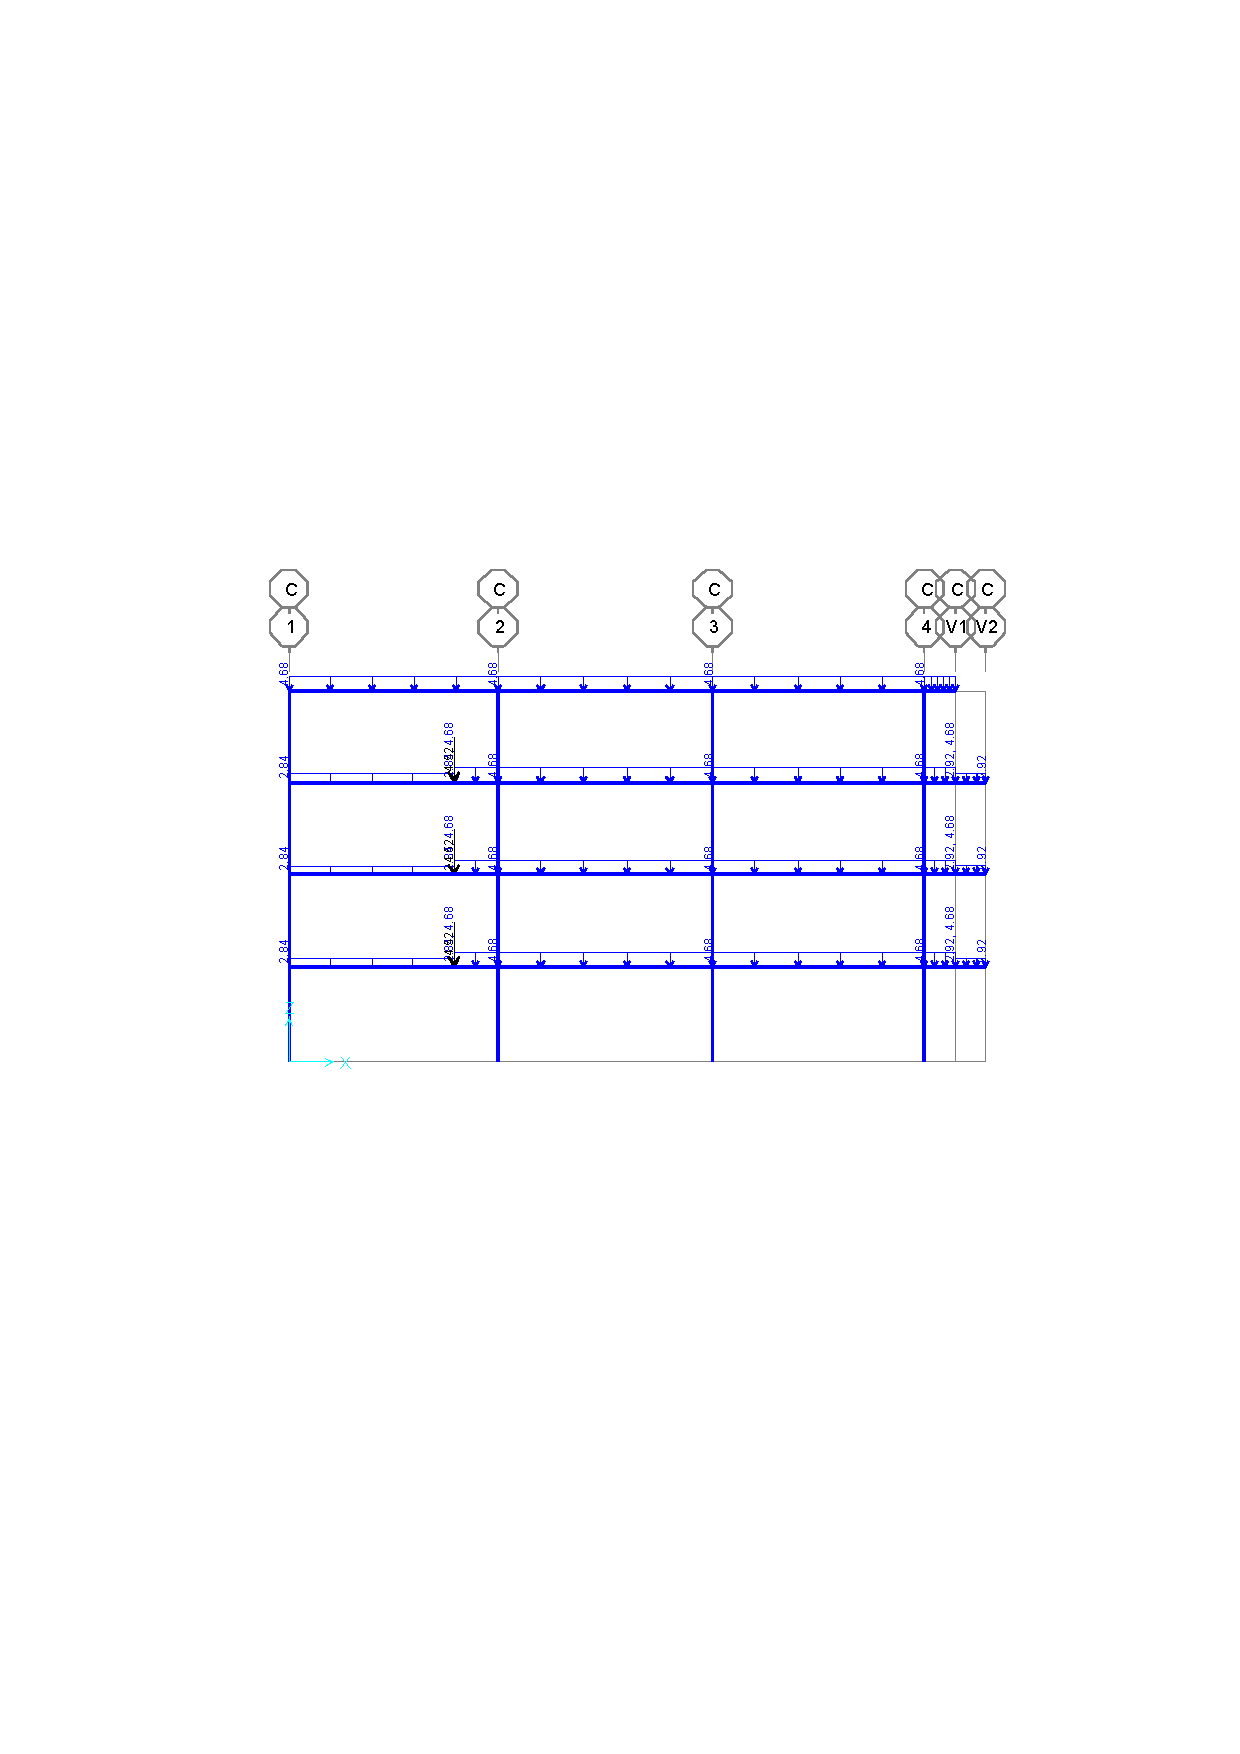
\includegraphics[scale=0.75]{images/CV 2.0/VCL.pdf}
    \caption{Esquema de carga viva viga en el eje C}
    \label{fig:EsqVigaEjeCV}
\end{figure}

\begin{figure}[H]
    \centering
    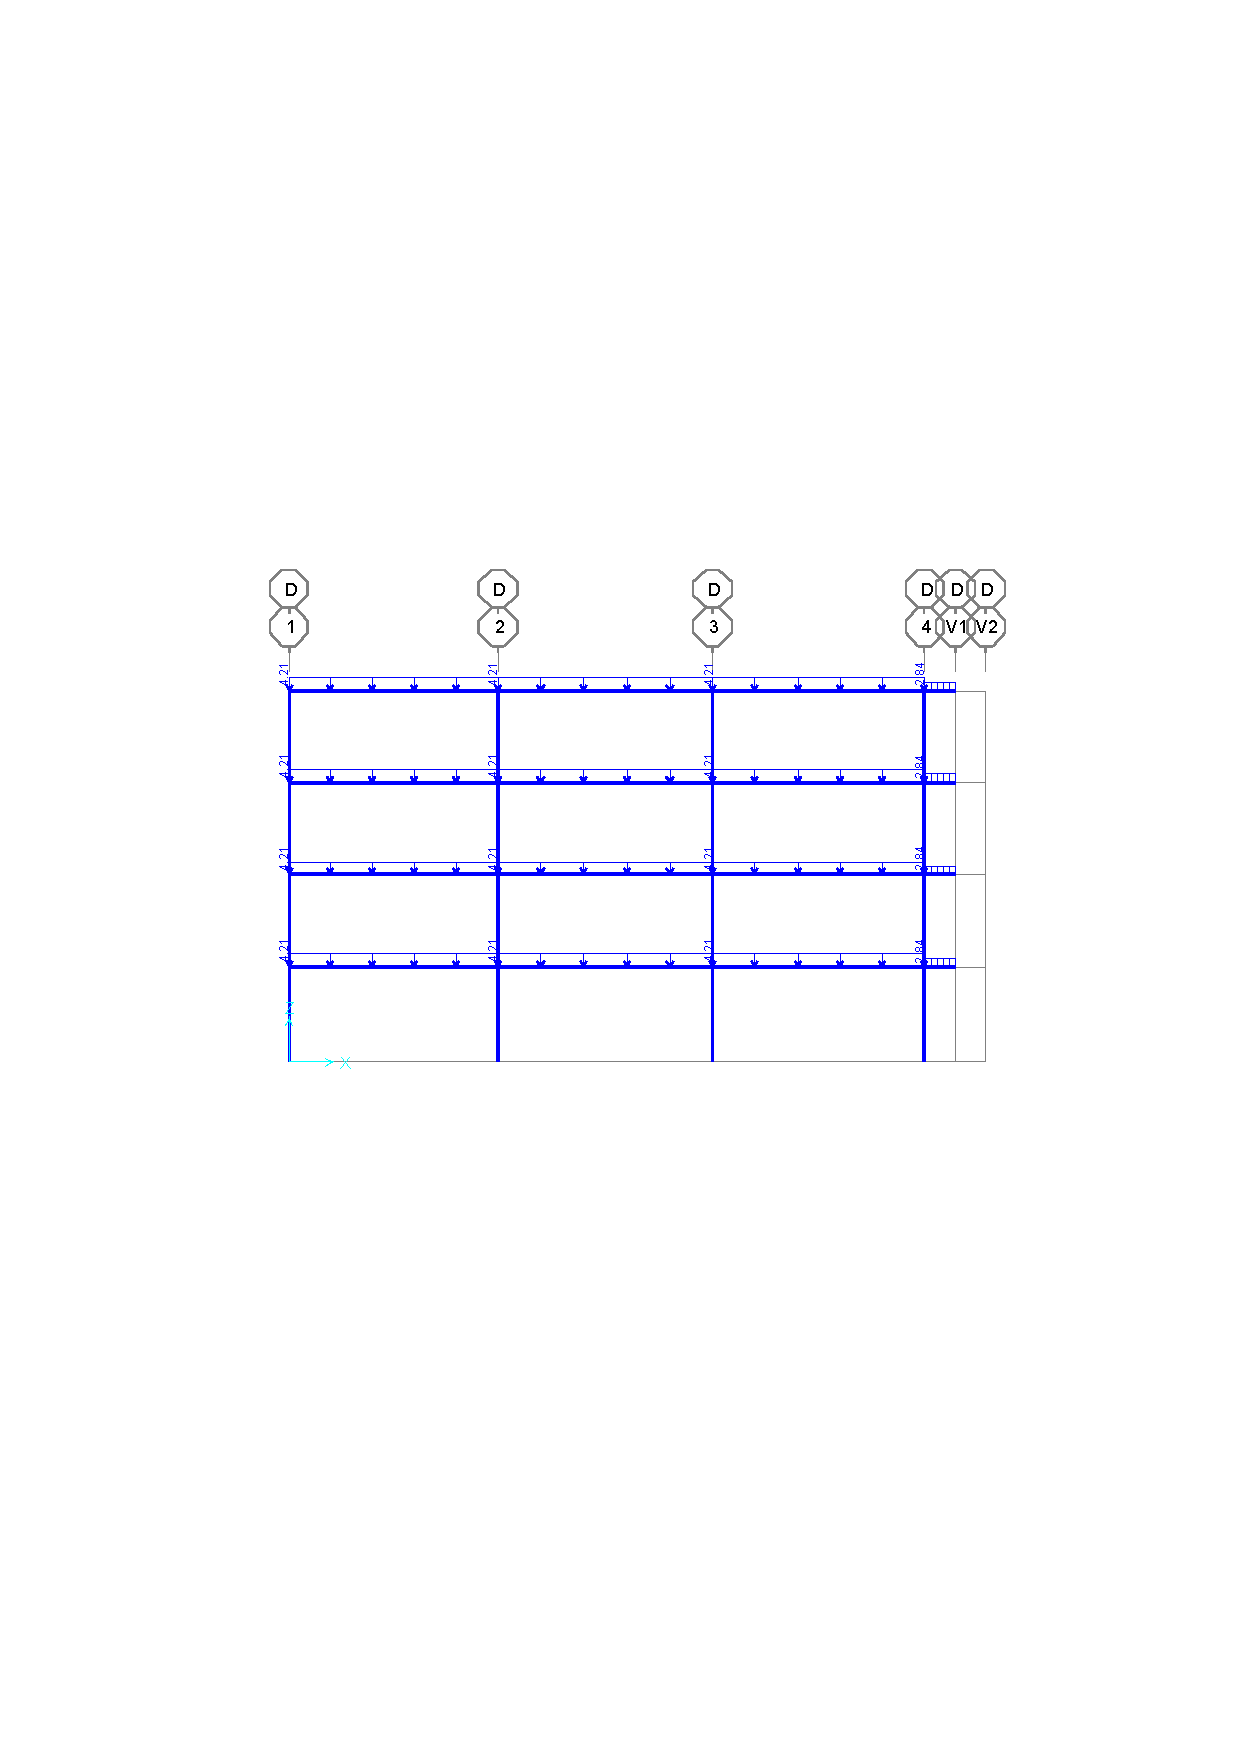
\includegraphics[scale=0.75]{images/CV 2.0/VDL.pdf}
    \caption{Esquema de carga viva viga en el eje D}
    \label{fig:EsqVigaEjeDV}
\end{figure}
%%%%7- viguetas 
\newpage
\section{Análisis y diseño de viguetas}
\subsection{Carga muerta y viva. Carga mayorada}

En la siguiente tabla se presenta un resumen de las cargas de la edificación, se tiene una carga mayorada 1.2D+1.6L
% Table generated by Excel2LaTeX from sheet 'Diagramas'
\begin{table}[H]
  \centering
  
    \begin{tabular}{|l|c|c|}
    \hline
    \rowcolor[rgb]{ .886,  .937,  .855} \multicolumn{3}{|c|}{\textbf{Resumen de cargas}} \bigstrut\\
    \hline
    \rowcolor[rgb]{ .886,  .937,  .855}     & \textbf{entrepiso} & \textbf{cubierta } \bigstrut\\
    \hline
    \rowcolor[rgb]{ .886,  .937,  .855} \textbf{$W_{D} (kN/m^2)$} & \cellcolor[rgb]{ 1,  1,  1}7.50 & \cellcolor[rgb]{ 1,  1,  1}5.37 \bigstrut\\
    \hline
    \rowcolor[rgb]{ .886,  .937,  .855} \textbf{$W_{L} (kN/m^2)$} & \cellcolor[rgb]{ 1,  1,  1}1.80 & \cellcolor[rgb]{ 1,  1,  1}1.8 \bigstrut\\
    \hline
    \rowcolor[rgb]{ .886,  .937,  .855} \textbf{$W_{U} (kN/m^2)$} & \cellcolor[rgb]{ 1,  1,  0}11.88 & \cellcolor[rgb]{ 1,  1,  0}9.32 \bigstrut\\
    \hline
    \end{tabular}%
    \caption{Carga muerta y viva del piso tipo y cubierta}
  \label{tab:addlabel}%
\end{table}%


Teniendo en cuenta la separación $S_{v}$ de cada una de las viguetas se determinan las siguientes cargas $q_{u}$ para cada uno de estas, tanto de entrepiso como de cubierta, las cuales se presentan a continuación:

% Table generated by Excel2LaTeX from sheet 'Diagramas'
\begin{table}[H]
  \centering
 
\begin{tabular}{|c|c|c|c|c|c|c|} 
\hhline{~------|}
\multicolumn{1}{c|}{}                           & \multicolumn{6}{c|}{{\cellcolor[rgb]{0.741,0.89,0.741}}\textbf{ENTREPISO}}                                                                                                                                                                                                                                       \\ 
\hhline{~------|}
\multicolumn{1}{c|}{}                           & \multicolumn{6}{c|}{{\cellcolor[rgb]{0.741,0.89,0.741}}\textbf{1.2D+1.6L}}                                                                                                                                                                                                                                       \\ 
\hhline{~------|}
\multicolumn{1}{c|}{}                           & {\cellcolor[rgb]{0.741,0.89,0.741}}\textbf{1-1'} & {\cellcolor[rgb]{0.741,0.89,0.741}}\textbf{1'-2} & {\cellcolor[rgb]{0.741,0.89,0.741}}\textbf{2-3} & {\cellcolor[rgb]{0.741,0.89,0.741}}\textbf{3-4} & {\cellcolor[rgb]{0.741,0.89,0.741}}\textbf{4-V41} & {\cellcolor[rgb]{0.741,0.89,0.741}}\textbf{4-V42}  \\ 
\hline
{\cellcolor[rgb]{0.741,0.89,0.741}}\textbf{VT1} & ~                                                & ~                                                & 7.43                                            & ~                                               & ~                                                 & ~                                                  \\ 
\hline
{\cellcolor[rgb]{0.741,0.89,0.741}}\textbf{VT2} & 12.36                                            & 12.36                                            & 12.36                                           & 12.36                                           & ~                                                 & ~                                                  \\ 
\hline
{\cellcolor[rgb]{0.741,0.89,0.741}}\textbf{VT3} & ~                                                & 13.31                                            & 8.61                                            & 13.31                                           & 13.31                                             & 13.31                                              \\ 
\hline
{\cellcolor[rgb]{0.741,0.89,0.741}}\textbf{VT4} & ~                                                & 13.31                                            & ~                                               & ~                                               & ~                                                 & ~                                                  \\ 
\hline
{\cellcolor[rgb]{0.741,0.89,0.741}}\textbf{VT5} & ~                                                & ~                                                & 10.99                                           & ~                                               & ~                                                 & ~                                                  \\ 
\hline
{\cellcolor[rgb]{0.741,0.89,0.741}}\textbf{VT6} & ~                                                & ~                                                & ~                                               & 13.31                                           & 13.31                                             & 13.31                                              \\ 
\hline
{\cellcolor[rgb]{0.741,0.89,0.741}}\textbf{VT7} & 12.83                                            & 12.83                                            & 12.83                                           & 12.83                                           & 12.83                                             & ~                                                  \\
\hline
\end{tabular}

     \caption{Cargas de viguetas para el piso-tipo }
  \label{tab:VTAPT}
  %
\end{table}%


% Table generated by Excel2LaTeX from sheet 'Diagramas'
\begin{table}[H]
  \centering
  % Table generated by Excel2LaTeX from sheet 'Diagramas'
\begin{tabular}{|c|c|c|c|c|c|c|} 
\hhline{~------|}
\multicolumn{1}{c|}{}                             & \multicolumn{6}{c|}{{\cellcolor[rgb]{0.741,0.89,0.741}}\textbf{CUBIERTA}}                                                                                                                                                                                                                                        \\ 
\hhline{~------|}
\multicolumn{1}{c|}{}                             & \multicolumn{6}{c|}{{\cellcolor[rgb]{0.741,0.89,0.741}}\textbf{1.2D+1.6L}}                                                                                                                                                                                                                                       \\ 
\hhline{~------|}
\multicolumn{1}{c|}{}                             & {\cellcolor[rgb]{0.741,0.89,0.741}}\textbf{1-1'} & {\cellcolor[rgb]{0.741,0.89,0.741}}\textbf{1'-2} & {\cellcolor[rgb]{0.741,0.89,0.741}}\textbf{2-3} & {\cellcolor[rgb]{0.741,0.89,0.741}}\textbf{3-4} & {\cellcolor[rgb]{0.741,0.89,0.741}}\textbf{4-V41} & {\cellcolor[rgb]{0.741,0.89,0.741}}\textbf{4-V42}  \\ 
\hline
{\cellcolor[rgb]{0.741,0.89,0.741}}\textbf{VT1}   & ~                                                & ~                                                & 5.83                                            & ~                                               & ~                                                 & ~                                                  \\ 
\hline
{\cellcolor[rgb]{0.741,0.89,0.741}}\textbf{VT2}   & 9.70                                             & 9.70                                             & 9.70                                            & 9.70                                            & ~                                                 & ~                                                  \\ 
\hline
{\cellcolor[rgb]{0.741,0.89,0.741}}\textbf{VT7 '} & 10.44                                            & 10.44                                            & 6.76                                            & 10.44                                           & 10.44                                             & ~                                                  \\ 
\hline
{\cellcolor[rgb]{0.741,0.89,0.741}}\textbf{VT7}   & 10.07                                            & 10.07                                            & 10.07                                           & 10.07                                           & 10.07                                             & ~                                                  \\ 
\hline
{\cellcolor[rgb]{0.741,0.89,0.741}}\textbf{VT8}   & 10.44                                            & 10.44                                            & ~                                               & ~                                               & ~                                                 & ~                                                  \\ 
\hline
{\cellcolor[rgb]{0.741,0.89,0.741}}\textbf{VT9}   & ~                                                & ~                                                & 8.62                                            & ~                                               & ~                                                 & ~                                                  \\ 
\hline
{\cellcolor[rgb]{0.741,0.89,0.741}}\textbf{VT10}  & ~                                                & ~                                                & ~                                               & 10.44                                           & 10.44                                             & ~                                                  \\
\hline
\end{tabular}
    \caption{Cargas de viguetas para cubierta}
  \label{tab:loadcub}%
\end{table}%

La vigueta \textbf{VT7'} corresponde a la vigueta 7, adyacente a la zona de los vacíos del ascensor y de la escalera.


\subsection{Diagramas de carga, cortante y momento de las viguetas}
A continuación se presentan los diagramas de carga, cortante y momento de cada una de las viguetas del proyecto para 1.2D+1.6L

\subsubsection{Viguetas piso tipo}
    \begin{itemize}
        \item \textbf{Vigueta 1}\\
            \begin{figure}[H]
                \centering
                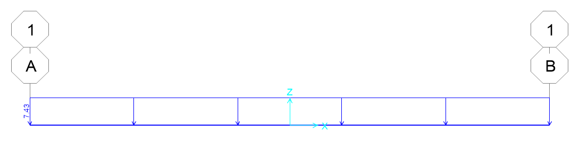
\includegraphics[width=0.9\linewidth]{images/viguetas/VT1 EP.png}
                \caption{Diagrama de carga (1.2D+1.6L) para la vigueta VT1 de entrepiso}
                \label{fig:W VT1 EP}
            \end{figure}
            
            \begin{figure}[H]
                \centering
                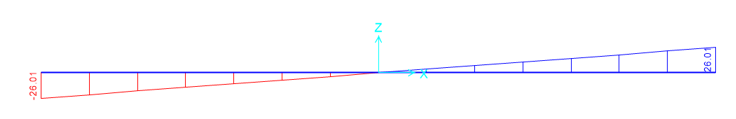
\includegraphics[width=0.9\linewidth]{images/viguetas/CORT VT1 EP.png}
                \caption{Diagrama de Cortante para la vigueta VT1 de entrepiso}
                \label{fig:v VT1 EP}
            \end{figure}
            
             \begin{figure}[H]
                \centering
                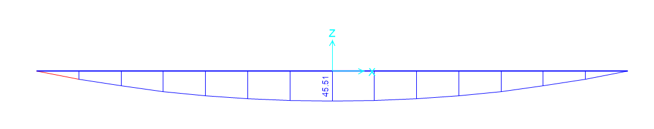
\includegraphics[width=0.9\linewidth]{images/viguetas/MOM VT1 EP.png}
                \caption{Diagrama de momento para la vigueta VT1 de entrepiso}
                \label{fig:M VT1 EP}
            \end{figure}
            
            \item \textbf{Vigueta 2}\\
            \begin{figure}[H]
                \centering
                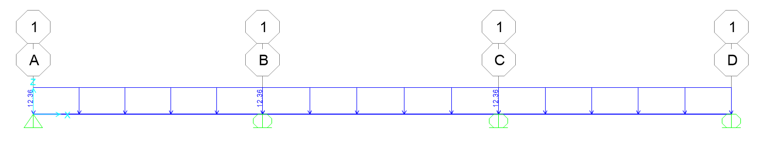
\includegraphics[width=0.9\linewidth]{images/viguetas/VT2 EP.png}
                \caption{Diagrama de carga (1.2D+1.6L) para la vigueta VT2 de entrepiso}
                \label{fig:W VT2 EP}
            \end{figure}
            
            \begin{figure}[H]
                \centering
                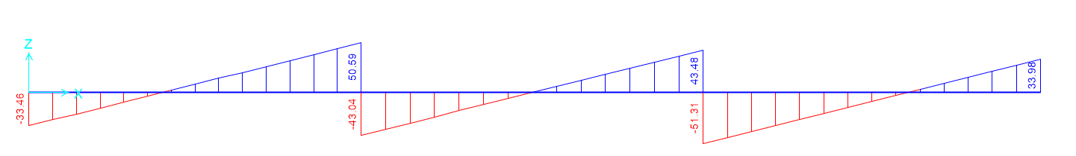
\includegraphics[width=0.9\linewidth]{images/viguetas/CORT VT2 EP.png} 
                \caption{Diagrama de Cortante para la vigueta VT2 de entrepiso}
                \label{fig:v VT2 EP}
            \end{figure}
            
             \begin{figure}[H]
                \centering
                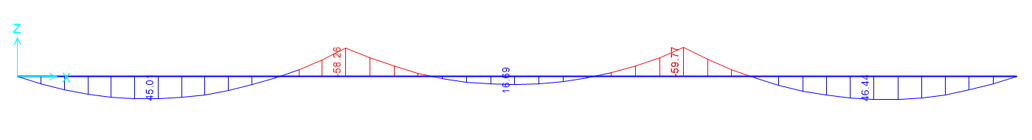
\includegraphics[width=0.9\linewidth]{images/viguetas/MOM VT2 EP.png} 
                \caption{Diagrama de momento para la vigueta VT2 de entrepiso}
                \label{fig:M VT2 EP}
            \end{figure}
            
             \item \textbf{Vigueta 3}\\
            \begin{figure}[H]
                \centering
                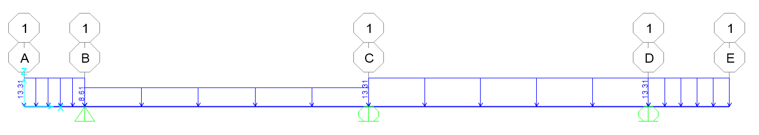
\includegraphics[width=0.9\linewidth]{images/viguetas/VT3 EP.png} 
                \caption{Diagrama de carga (1.2D+1.6L) para la vigueta VT3 de entrepiso}
                \label{fig:W VT3 EP}
            \end{figure}
            
            \begin{figure}[H]
                \centering
                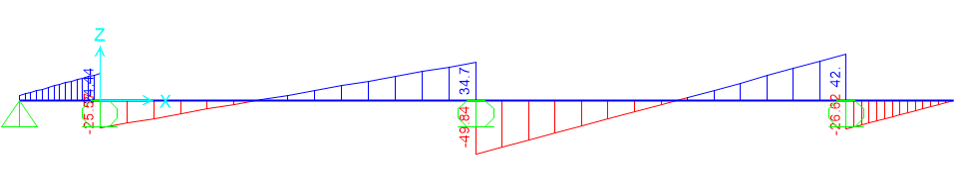
\includegraphics[width=0.9\linewidth]{images/viguetas/CORT VT3 EP.png} 
                \caption{Diagrama de Cortante para la vigueta VT3 de entrepiso}
                \label{fig:v VT3 EP}
            \end{figure}
            
             \begin{figure}[H]
                \centering
                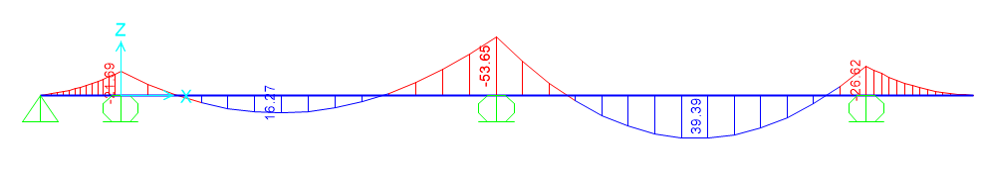
\includegraphics[width=0.9\linewidth]{images/viguetas/MOM VT3 EP.png} 
                \caption{Diagrama de momento para la vigueta VT3 de entrepiso}
                \label{fig:M VT3 EP}
            \end{figure}
            
            \item \textbf{Vigueta 4}\\
            \begin{figure}[H]
                \centering
                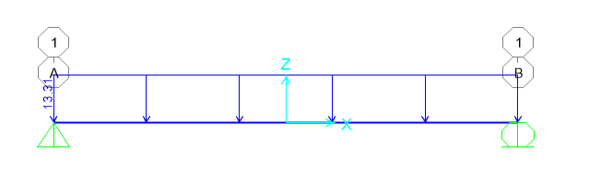
\includegraphics[width=0.9\linewidth]{images/viguetas/VT4 EP.png}
                \caption{Diagrama de carga (1.2D+1.6L) para la vigueta VT4 de entrepiso}
                \label{fig:W VT4 EP}
            \end{figure}
            
            \begin{figure}[H]
                \centering
                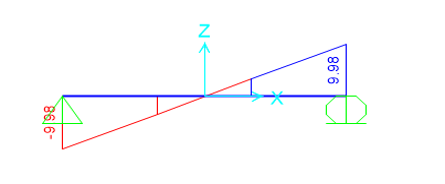
\includegraphics[width=0.9\linewidth]{images/viguetas/CORT VT4 EP.png} 
                \caption{Diagrama de Cortante para la vigueta VT4 de entrepiso}
                \label{fig:v VT4 EP}
            \end{figure}
            
             \begin{figure}[H]
                \centering
                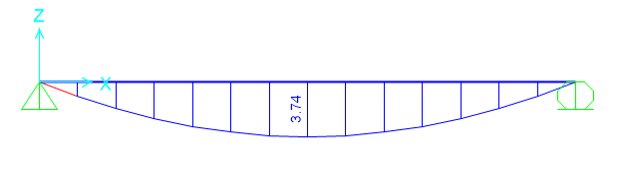
\includegraphics[width=0.9\linewidth]{images/viguetas/MOM VT4 EP.png} 
                \caption{Diagrama de momento para la vigueta VT4 de entrepiso}
                \label{fig:M VT4 EP}
            \end{figure}
            
            
            \item \textbf{Vigueta 5}\\
            \begin{figure}[H]
                \centering
                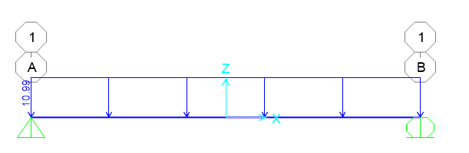
\includegraphics[width=0.9\linewidth]{images/viguetas/VT5 EP.png} 
                \caption{Diagrama de carga (1.2D+1.6L) para la vigueta VT5 de entrepiso}
                \label{fig:W VT5 EP}
            \end{figure}
            
            \begin{figure}[H]
                \centering
                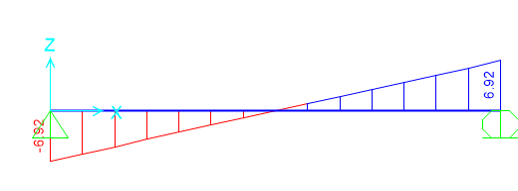
\includegraphics[width=0.9\linewidth]{images/viguetas/CORT VT5 EP.png} 
                \caption{Diagrama de Cortante para la vigueta VT5 de entrepiso}
                \label{fig:v VT5 EP}
            \end{figure}
            
             \begin{figure}[H]
                \centering
                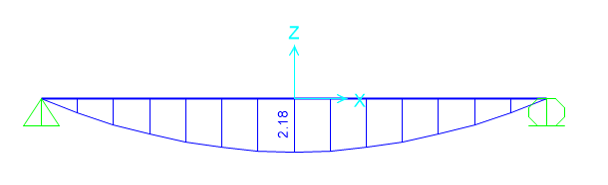
\includegraphics[width=0.9\linewidth]{images/viguetas/MOM VT5 EP.png} 
                \caption{Diagrama de momento para la vigueta VT5 de entrepiso}
                \label{fig:M VT5 EP}
            \end{figure}
            
            \item \textbf{Vigueta 6}\\
            \begin{figure}[H]
                \centering
                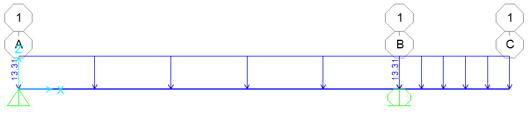
\includegraphics[width=0.9\linewidth]{images/viguetas/VT6 EP.png} 
                \caption{Diagrama de carga (1.2D+1.6L) para la vigueta VT6 de entrepiso}
                \label{fig:W VT6 EP}
            \end{figure}
            
            \begin{figure}[H]
                \centering
                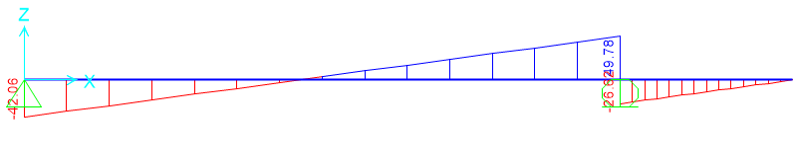
\includegraphics[width=0.9\linewidth]{images/viguetas/CORT VT6 EP.png} 
                \caption{Diagrama de Cortante para la vigueta VT6 de entrepiso}
                \label{fig:v VT6 EP}
            \end{figure}
            
             \begin{figure}[H]
                \centering
                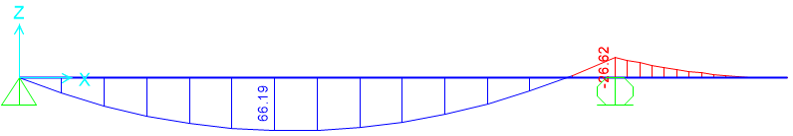
\includegraphics[width=0.9\linewidth]{images/viguetas/MOM VT6 EP.png} 
                \caption{Diagrama de momento para la vigueta VT6 de entrepiso}
                \label{fig:M VT6 EP}
            \end{figure}
            
            \item \textbf{Vigueta 7}\\
            \begin{figure}[H]
                \centering
                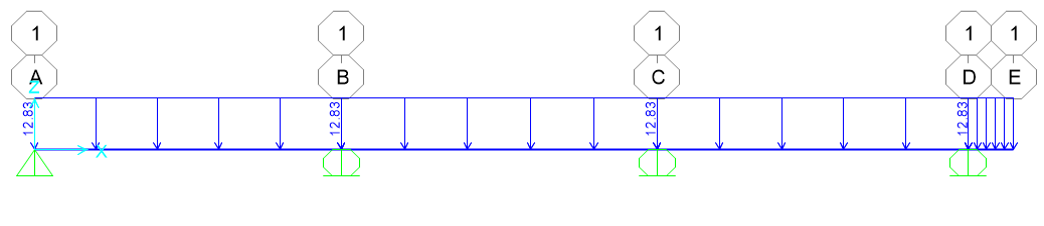
\includegraphics[width=0.9\linewidth]{images/viguetas/VT7 EP.png} 
                \caption{Diagrama de carga (1.2D+1.6L) para la vigueta VT7 de entrepiso}
                \label{fig:W VT7 EP}
            \end{figure}
            
            \begin{figure}[H]
                \centering
                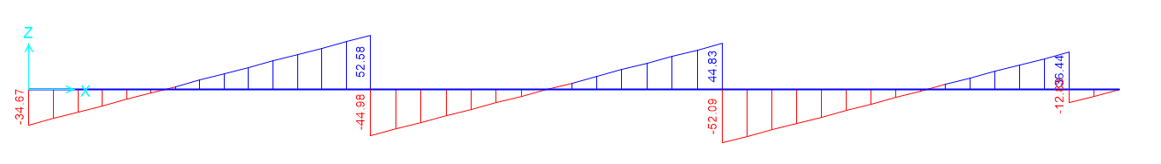
\includegraphics[width=0.9\linewidth]{images/viguetas/CORT VT7 EP.png}
                \caption{Diagrama de Cortante para la vigueta VT7 de entrepiso}
                \label{fig:v VT7 EP}
            \end{figure}
            
             \begin{figure}[H]
                \centering
                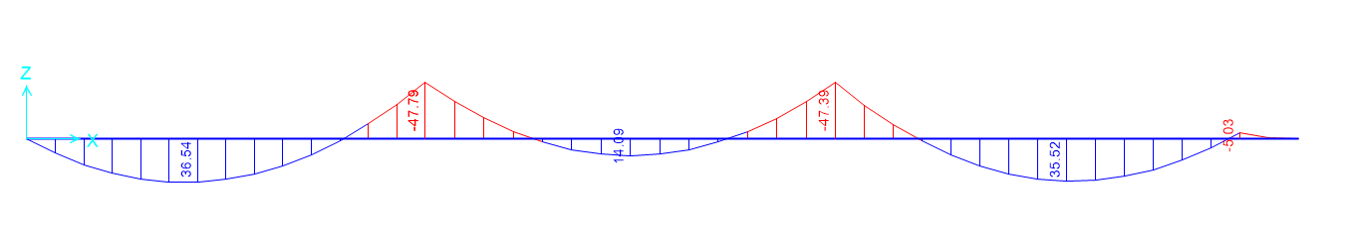
\includegraphics[width=0.9\linewidth]{images/viguetas/MOM VT7 CUB.png} 
                \caption{Diagrama de momento para la vigueta VT7 de entrepiso}
                \label{fig:M VT7 EP}
            \end{figure}
\end{itemize}

\subsubsection{Viguetas cubierta}

\begin{itemize}
    \item \textbf{Vigueta 1}\\
    \begin{figure}[H]
                \centering
                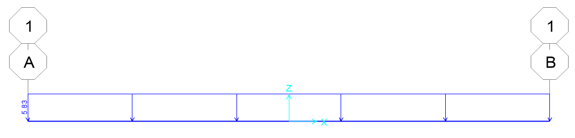
\includegraphics[width=0.9\linewidth]{images/viguetas/VT1 CUB.png} 
                \caption{Diagrama de carga (1.2D+1.6L) para la vigueta VT1 de cubierta}
                \label{fig:W VT1 CUB}
            \end{figure}
            
            \begin{figure}[H]
                \centering
                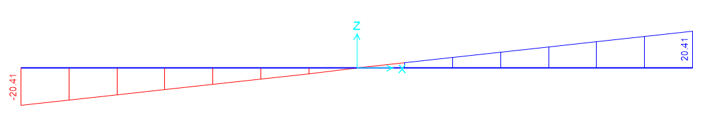
\includegraphics[width=0.9\linewidth]{images/viguetas/CORT VT1 CUB.png}
                \caption{Diagrama de Cortante para la vigueta VT1 de cubierta}
                \label{fig:v VT7 CUB}
            \end{figure}
            
             \begin{figure}[H]
                \centering
                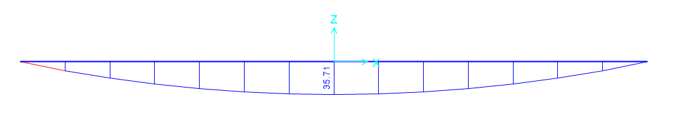
\includegraphics[width=0.9\linewidth]{images/viguetas/MOM VT1 CUB.png} 
                \caption{Diagrama de momento para la vigueta VT1 de cubierta}
                \label{fig:M VT1 CUB}
            \end{figure}
        
        \item \textbf{Vigueta 2}\\
        \begin{figure}[H]
                \centering
                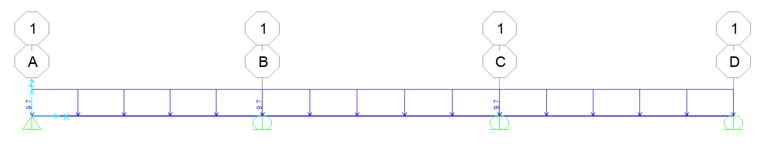
\includegraphics[width=0.9\linewidth]{images/viguetas/VT2 CUB.png} 
                \caption{Diagrama de carga (1.2D+1.6L) para la vigueta VT2 de cubierta}
                \label{fig:W VT2 CUB}
            \end{figure}
            
            \begin{figure}[H]
                \centering
                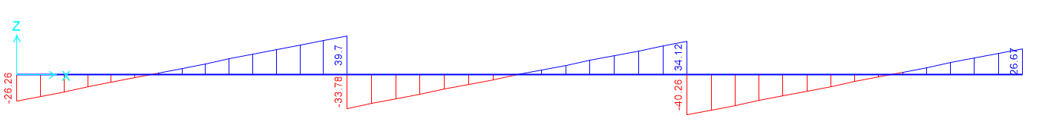
\includegraphics[width=0.9\linewidth]{images/viguetas/CORT VT2 CUB.png}
                \caption{Diagrama de Cortante para la vigueta VT2 de cubierta}
                \label{fig:v VT2 CUB}
            \end{figure}
            
             \begin{figure}[H]
                \centering
                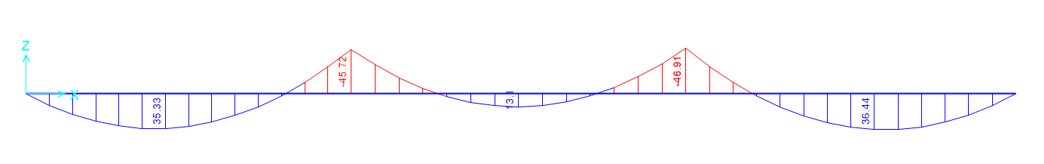
\includegraphics[width=0.9\linewidth]{images/viguetas/MOM VT2 CUB.png} 
                \caption{Diagrama de momento para la vigueta VT2 de cubierta}
                \label{fig:M VT2 CUB}
            \end{figure}
            
            \item \textbf{Vigueta 7'}\\
        \begin{figure}[H]
                \centering
                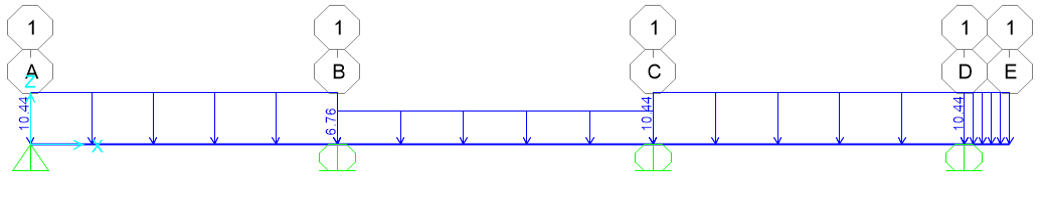
\includegraphics[width=0.9\linewidth]{images/viguetas/VT7 CUB'.png} 
                \caption{Diagrama de carga (1.2D+1.6L) para la vigueta VT7' de cubierta}
                \label{fig:W VT7' CUB}
            \end{figure}
            
            \begin{figure}[H]
                \centering
                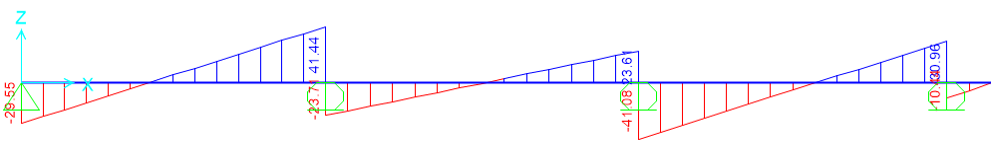
\includegraphics[width=0.9\linewidth]{images/viguetas/CORT VT 7 CUB'.png}
                \caption{Diagrama de Cortante para la vigueta VT7' de cubierta}
                \label{fig:v VT7' CUB}
            \end{figure}
            
             \begin{figure}[H]
                \centering
                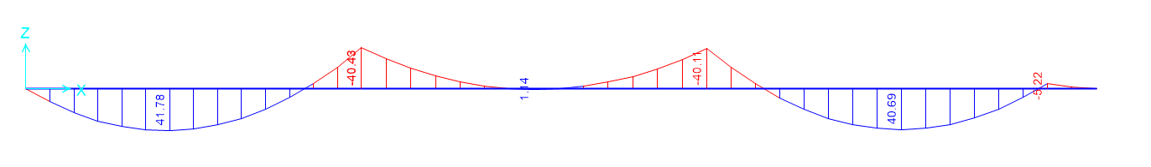
\includegraphics[width=0.9\linewidth]{images/viguetas/MOM VT7 CUB'.png} 
                \caption{Diagrama de momento para la vigueta VT7' de cubierta}
                \label{fig:M VT7' CUB}
            \end{figure}
            
            
               \item \textbf{Vigueta 7}\\
        \begin{figure}[H]
                \centering
                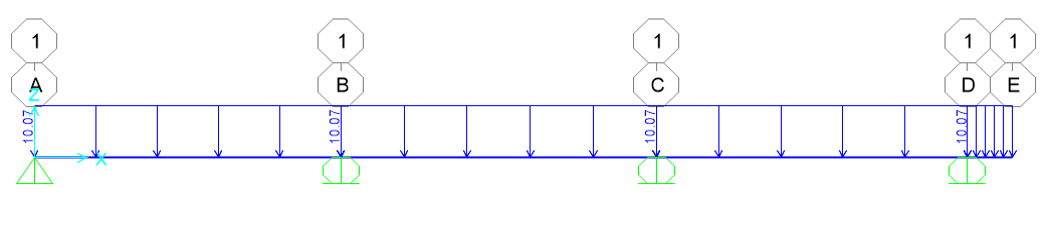
\includegraphics[width=0.9\linewidth]{images/viguetas/VT7 CUB.png} 
                \caption{Diagrama de carga (1.2D+1.6L) para la vigueta VT7 de cubierta}
                \label{fig:W VT7 CUB}
            \end{figure}
            
            \begin{figure}[H]
                \centering
                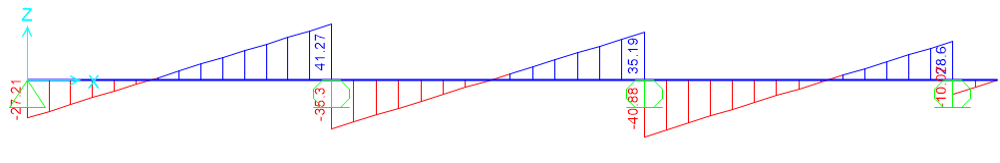
\includegraphics[width=0.9\linewidth]{images/viguetas/CORT VT 7 CUB.png}
                \caption{Diagrama de Cortante para la vigueta VT7 de cubierta}
                \label{fig:v VT7 CUB}
            \end{figure}
            
             \begin{figure}[H]
                \centering
                \includegraphics[width=0.9\linewidth]{images/viguetas/MOM VT7 CUB.png} 
                \caption{Diagrama de momento para la vigueta VT7 de cubierta}
                \label{fig:M VT7 CUB}
            \end{figure}
            
              \item \textbf{Vigueta 8}\\
        \begin{figure}[H]
                \centering
                \includegraphics[width=0.9\linewidth]{images/viguetas/VT8 CUB.png} 
                \caption{Diagrama de carga (1.2D+1.6L) para la vigueta VT8 de cubierta}
                \label{fig:W VT8 CUB}
            \end{figure}
            
            \begin{figure}[H]
                \centering
                \includegraphics[width=0.9\linewidth]{images/viguetas/CORT VT8 CUB.png}
                \caption{Diagrama de Cortante para la vigueta VT8 de cubierta}
                \label{fig:v VT8 CUB}
            \end{figure}
            
             \begin{figure}[H]
                \centering
                \includegraphics[width=0.9\linewidth]{images/viguetas/MOM VT8 CUB.png} 
                \caption{Diagrama de momento para la vigueta VT8 de cubierta}
                \label{fig:M VT8 CUB}
            \end{figure}
            
            
             \item \textbf{Vigueta 9}\\
        \begin{figure}[H]
                \centering
                \includegraphics[width=0.9\linewidth]{images/viguetas/VT9 CUB.png} 
                \caption{Diagrama de carga (1.2D+1.6L) para la vigueta VT9 de cubierta}
                \label{fig:W VT9 CUB}
            \end{figure}
            
            \begin{figure}[H]
                \centering
                \includegraphics[width=0.9\linewidth]{images/viguetas/CORT V9 CUB.png}
                \caption{Diagrama de Cortante para la vigueta VT9 de cubierta}
                \label{fig:v VT9 CUB}
            \end{figure}
            
             \begin{figure}[H]
                \centering
                \includegraphics[width=0.9\linewidth]{images/viguetas/MOM VT9 CUB.png} 
                \caption{Diagrama de momento para la vigueta VT9 de cubierta}
                \label{fig:M VT9 CUB}
            \end{figure}
            
             \item \textbf{Vigueta 10}\\
        \begin{figure}[H]
                \centering
                \includegraphics[width=0.9\linewidth]{images/viguetas/VT10 CUB.png} 
                \caption{Diagrama de carga (1.2D+1.6L) para la vigueta VT10 de cubierta}
                \label{fig:W VT10 CUB}
            \end{figure}
            
            \begin{figure}[H]
                \centering
                \includegraphics[width=0.9\linewidth]{images/viguetas/CORT VT10 CUB.png}
                \caption{Diagrama de Cortante para la vigueta VT10 de cubierta}
                \label{fig:v VT10 CUB}
            \end{figure}
            
             \begin{figure}[H]
                \centering
                \includegraphics[width=0.9\linewidth]{images/viguetas/MOM VT10 CUB.png} 
                \caption{Diagrama de momento para la vigueta VT10 de cubierta}
                \label{fig:M VT10 CUB}
            \end{figure}
    
\end{itemize}

\subsubsection{Vigas auxiliares}
De igual manera, para diseñar las vigas auxiliares se utilizaron las mismas combinaciones de carga y a continuación se muestran los diagramas de carga, cortante y momento para cada una de las vigas auxiliares del proyecto:

\subsubsection{Vigas auxiliares piso tipo}
\begin{itemize}
        \item \textbf{Viga auxiliar 10}\\
            \begin{figure}[H]
                \centering
                \includegraphics[width=0.9\linewidth]{images/viguetas/V-10.png}
                \caption{Diagrama de carga (1.2D+1.6L) para la viga auxiliar V-10 de entrepiso}
                \label{fig:W V-10 EP}
            \end{figure}
            
            \begin{figure}[H]
                \centering
                \includegraphics[width=0.9\linewidth]{images/viguetas/CORT-10.png}
                \caption{Diagrama de cortante (1.2D+1.6L) para la viga auxiliar V-10 de entrepiso}
                \label{fig:Cort V-10 EP}
            \end{figure}
            
            \begin{figure}[H]
                \centering
                \includegraphics[width=0.9\linewidth]{images/viguetas/MOM-10.png}
                \caption{Diagrama de momento (1.2D+1.6L) para la viga auxiliar V-10 de entrepiso}
                \label{fig:MOm V-10 EP}
            \end{figure}
            
            \item \textbf{Viga auxiliar 11}\\
            \begin{figure}[H]
                \centering
                \includegraphics[width=0.9\linewidth]{images/viguetas/V-11.png}
                \caption{Diagrama de carga (1.2D+1.6L) para la viga auxiliar V-11 de entrepiso}
                \label{fig:W V-11 EP}
            \end{figure}
            
            \begin{figure}[H]
                \centering
                \includegraphics[width=0.9\linewidth]{images/viguetas/CORT-11.png}
                \caption{Diagrama de cortante (1.2D+1.6L) para la viga auxiliar V-11 de entrepiso}
                \label{fig:Cort V-11 EP}
            \end{figure}
            
            \begin{figure}[H]
                \centering
                \includegraphics[width=0.9\linewidth]{images/viguetas/MOM-11.png}
                \caption{Diagrama de momento (1.2D+1.6L) para la viga auxiliar V-11 de entrepiso}
                \label{fig:Mom V-11 EP}
            \end{figure}
            
            \item \textbf{Viga auxiliar 12}\\
            \begin{figure}[H]
                \centering
                \includegraphics[width=0.9\linewidth]{images/viguetas/V-12.png}
                \caption{Diagrama de carga (1.2D+1.6L) para la viga auxiliar V-12 de entrepiso}
                \label{fig:W V-12 EP}
            \end{figure}
            
            \begin{figure}[H]
                \centering
                \includegraphics[width=0.9\linewidth]{images/viguetas/CORT-12.png}
                \caption{Diagrama de cortante (1.2D+1.6L) para la viga auxiliar V-12 de entrepiso}
                \label{fig:Cort V-12 EP}
            \end{figure}
            
            \begin{figure}[H]
                \centering
                \includegraphics[width=0.9\linewidth]{images/viguetas/MOM-12.png}
                \caption{Diagrama de momento (1.2D+1.6L) para la viga auxiliar V-12 de entrepiso}
                \label{fig:Mom V-12 EP}
            \end{figure}
            
            
            \item \textbf{Viga auxiliar 13}\\
            \begin{figure}[H]
                \centering
                \includegraphics[width=0.9\linewidth]{images/viguetas/V-13.png}
                \caption{Diagrama de carga (1.2D+1.6L) para la viga auxiliar V-13 de entrepiso}
                \label{fig:W V-13 EP}
            \end{figure}
            
            \begin{figure}[H]
                \centering
                \includegraphics[width=0.9\linewidth]{images/viguetas/CORT-13.png}
                \caption{Diagrama de cortante (1.2D+1.6L) para la viga auxiliar V-13 de entrepiso}
                \label{fig:Cort V-13 EP}
            \end{figure}
            
            \begin{figure}[H]
                \centering
                \includegraphics[width=0.9\linewidth]{images/viguetas/MOM-13.png}
                \caption{Diagrama de momento (1.2D+1.6L) para la viga auxiliar V-13 de entrepiso}
                \label{fig:Mom V-13 EP}
            \end{figure}
            
            \item \textbf{Viga auxiliar 14}\\
            \begin{figure}[H]
                \centering
                \includegraphics[width=0.9\linewidth]{images/viguetas/V-14.png}
                \caption{Diagrama de carga (1.2D+1.6L) para la viga auxiliar V-14 de entrepiso}
                \label{fig:W V-14 EP}
            \end{figure}
            
            \begin{figure}[H]
                \centering
                \includegraphics[width=0.9\linewidth]{images/viguetas/CORT-14.png}
                \caption{Diagrama de cortante (1.2D+1.6L) para la viga auxiliar V-14 de entrepiso}
                \label{fig:Cort V-14 EP}
            \end{figure}
            
            \begin{figure}[H]
                \centering
                \includegraphics[width=0.9\linewidth]{images/viguetas/MOM-14.png}
                \caption{Diagrama de momento (1.2D+1.6L) para la viga auxiliar V-14 de entrepiso}
                \label{fig:Mom V-14 EP}
            \end{figure}
            
\end{itemize}




\subsubsection{Vigas auxiliares cubierta}
\begin{itemize}
        % \item \textbf{Viga auxiliar 10}\\
        %     \begin{figure}[H]
        %         \centering
        %         \includegraphics[width=0.9\linewidth]{images/viguetas/V-10C.png}
        %         \caption{Diagrama de carga (1.2D+1.6L) para la viga auxiliar V-10 de cubierta}
        %         \label{fig:W V-10 EP}
        %     \end{figure}
            
        %     \begin{figure}[H]
        %         \centering
        %         \includegraphics[width=0.9\linewidth]{images/viguetas/CORT-10C.png}
        %         \caption{Diagrama de cortante (1.2D+1.6L) para la viga auxiliar V-10 de cubierta}
        %         \label{fig:Cort V-10 EP}
        %     \end{figure}
            
        %     \begin{figure}[H]
        %         \centering
        %         \includegraphics[width=0.9\linewidth]{images/viguetas/MOM-10C.png}
        %         \caption{Diagrama de momento (1.2D+1.6L) para la viga auxiliar V-10 de cubierta}
        %         \label{fig:MOm V-10 EP}
        %     \end{figure}
            
            \item \textbf{Viga auxiliar 11}\\
            \begin{figure}[H]
                \centering
                \includegraphics[width=0.9\linewidth]{images/viguetas/V-11C.png}
                \caption{Diagrama de carga (1.2D+1.6L) para la viga auxiliar V-11 de cubierta}
                \label{fig:W V-11 EP}
            \end{figure}
            
            \begin{figure}[H]
                \centering
                \includegraphics[width=0.9\linewidth]{images/viguetas/CORT-11C.png}
                \caption{Diagrama de cortante (1.2D+1.6L) para la viga auxiliar V-11 de cubierta}
                \label{fig:Cort V-11 EP}
            \end{figure}
            
            \begin{figure}[H]
                \centering
                \includegraphics[width=0.9\linewidth]{images/viguetas/MOM-11C.png}
                \caption{Diagrama de momento (1.2D+1.6L) para la viga auxiliar V-11 de cubierta}
                \label{fig:Mom V-11 EP}
            \end{figure}
            
            \item \textbf{Viga auxiliar 12}\\
            \begin{figure}[H]
                \centering
                \includegraphics[width=0.9\linewidth]{images/viguetas/V-12C.png}
                \caption{Diagrama de carga (1.2D+1.6L) para la viga auxiliar V-12 de cubierta}
                \label{fig:W V-12 EP}
            \end{figure}
            
            \begin{figure}[H]
                \centering
                \includegraphics[width=0.9\linewidth]{images/viguetas/CORT-12C.png}
                \caption{Diagrama de cortante (1.2D+1.6L) para la viga auxiliar V-12 de cubierta}
                \label{fig:Cort V-12 EP}
            \end{figure}
            
            \begin{figure}[H]
                \centering
                \includegraphics[width=0.9\linewidth]{images/viguetas/MOM-12C.png}
                \caption{Diagrama de momento (1.2D+1.6L) para la viga auxiliar V-12 de cubierta}
                \label{fig:Mom V-12 EP}
            \end{figure}
            
            
            \item \textbf{Viga auxiliar 13}\\
            \begin{figure}[H]
                \centering
                \includegraphics[width=0.9\linewidth]{images/viguetas/V-13C.png}
                \caption{Diagrama de carga (1.2D+1.6L) para la viga auxiliar V-13 de cubierta}
                \label{fig:W V-13 EP}
            \end{figure}
            
            \begin{figure}[H]
                \centering
                \includegraphics[width=0.9\linewidth]{images/viguetas/CORT-13C.png}
                \caption{Diagrama de cortante (1.2D+1.6L) para la viga auxiliar V-13 de cubierta}
                \label{fig:Cort V-13 EP}
            \end{figure}
            
            \begin{figure}[H]
                \centering
                \includegraphics[width=0.9\linewidth]{images/viguetas/MOM-13C.png}
                \caption{Diagrama de momento (1.2D+1.6L) para la viga auxiliar V-13 de cubierta}
                \label{fig:Mom V-13 EP}
            \end{figure}
            
            \item \textbf{Viga auxiliar 14}\\
            \begin{figure}[H]
                \centering
                \includegraphics[width=0.9\linewidth]{images/viguetas/V-14C.png}
                \caption{Diagrama de carga (1.2D+1.6L) para la viga auxiliar V-14 de cubierta}
                \label{fig:W V-14 EP}
            \end{figure}
            
            \begin{figure}[H]
                \centering
                \includegraphics[width=0.9\linewidth]{images/viguetas/CORT-14C.png}
                \caption{Diagrama de cortante (1.2D+1.6L) para la viga auxiliar V-14 de cubierta}
                \label{fig:Cort V-14 EP}
            \end{figure}
            
            \begin{figure}[H]
                \centering
                \includegraphics[width=0.9\linewidth]{images/viguetas/MOM-14C.png}
                \caption{Diagrama de momento (1.2D+1.6L) para la viga auxiliar V-14 de cubierta}
                \label{fig:Mom V-14 EP}
            \end{figure}
            
\end{itemize}

% FALTAN VIGAS AUXILIARES Y VIGUETA 7'
\newpage
\subsection{Diseño a cortante y diseño a flexión}

\subsubsection{Diseño a a flexión de viguetas}
\begin{itemize}
    \item \textbf{Piso Tipo}\\
      
        \vspace{1cm}
        % Table generated by Excel2LaTeX from sheet 'VTA 1'
\begin{table}[H]
  \centering
\resizebox{\linewidth}{!}{
    \    \begin{tabular}{|c|c|c|c|c|c|c|c|c|c|}
\cline{1-9}    \rowcolor[rgb]{ .859,  .859,  .859} \multicolumn{5}{|c|}{\textbf{VIGUETA VT1}} & \multicolumn{2}{c|}{\cellcolor[rgb]{ 1,  1,  1}\textbf{As suministrado}} & \multicolumn{2}{c|}{\cellcolor[rgb]{ 1,  1,  1}\textbf{Diseño}} & \multicolumn{1}{r}{\cellcolor[rgb]{ 1,  1,  1}} \bigstrut\\
    \hline
    \textbf{Distancia (m)} & \multicolumn{1}{p{6.855em}|}{\textbf{$M_{ SAP} (KN\cdot m)$}} & \multicolumn{1}{p{6.07em}|}{\textbf{$Mu (KN\cdot m)$}} & \textbf{$\rho$} & \textbf{$A_{s} (mm^2)$} & \textbf{$A_{s} (mm^2)$} & \textbf{cumple} & \textbf{Barra \#} & \textbf{Cantidad} & \textbf{Posición} \bigstrut\\
    \hline
    0   & 0.000 & 0.000 & 0.0033 & 146.667 & 387 & si  & 7   & 1   & Abajo \bigstrut\\
    \hline
    0.35 & 8.647 & 8.647 & 0.0033 & 146.667 & 387 & si  & 7   & 1   & Abajo \bigstrut\\
    \hline
    0.7 & 16.383 & 16.383 & 0.0033 & 146.667 & 387 & si  & 7   & 1   & Abajo \bigstrut\\
    \hline
    1.05 & 23.210 & 23.210 & 0.0045 & 199.914 & 387 & si  & 7   & 1   & Abajo \bigstrut\\
    \hline
    1.4 & 29.126 & 29.126 & 0.0057 & 252.864 & 387 & si  & 7   & 1   & Abajo \bigstrut\\
    \hline
    1.75 & 34.132 & 34.132 & 0.0068 & 298.360 & 387 & si  & 7   & 1   & Abajo \bigstrut\\
    \hline
    2.1 & 38.227 & 38.227 & 0.0076 & 336.077 & 387 & si  & 7   & 1   & Abajo \bigstrut\\
    \hline
    2.45 & 41.413 & 41.413 & 0.0083 & 365.730 & 387 & si  & 7   & 1   & Abajo \bigstrut\\
    \hline
    2.8 & 43.688 & 43.688 & 0.0088 & 387.085 & 510 & si  & 8   & 1   & Abajo \bigstrut\\
    \hline
    3.15 & 45.054 & 45.054 & 0.0091 & 399.971 & 510 & si  & 8   & 1   & Abajo \bigstrut\\
    \hline
    3.5 & 45.509 & 45.509 & 0.0092 & 404.278 & 510 & si  & 8   & 1   & Abajo \bigstrut\\
    \hline
    3.85 & 45.054 & 45.054 & 0.0091 & 399.971 & 510 & si  & 8   & 1   & Abajo \bigstrut\\
    \hline
    4.2 & 43.688 & 43.688 & 0.0088 & 387.085 & 510 & si  & 8   & 1   & Abajo \bigstrut\\
    \hline
    4.55 & 41.413 & 41.413 & 0.0083 & 365.730 & 387 & si  & 7   & 1   & Abajo \bigstrut\\
    \hline
    4.9 & 38.227 & 38.227 & 0.0076 & 336.077 & 387 & si  & 7   & 1   & Abajo \bigstrut\\
    \hline
    5.25 & 34.132 & 34.132 & 0.0068 & 298.360 & 387 & si  & 7   & 1   & Abajo \bigstrut\\
    \hline
    5.6 & 29.126 & 29.126 & 0.0057 & 252.864 & 387 & si  & 7   & 1   & Abajo \bigstrut\\
    \hline
    5.95 & 23.210 & 23.210 & 0.0045 & 199.914 & 387 & si  & 7   & 1   & Abajo \bigstrut\\
    \hline
    6.3 & 16.383 & 16.383 & 0.0033 & 146.667 & 387 & si  & 7   & 1   & Abajo \bigstrut\\
    \hline
    6.65 & 8.647 & 8.647 & 0.0033 & 146.667 & 387 & si  & 7   & 1   & Abajo \bigstrut\\
    \hline
    7   & 0.000 & 0.000 & 0.0033 & 146.667 & 387 & si  & 7   & 1   & Abajo \bigstrut\\
    \hline
    \end{tabular}%%
   }%
      \caption{Diseño por flexión de la vigueta 1 de entrepiso}
  \label{tab:F VT1 EP}%
\end{table}%

        

% \tiny  % Switch from 12pt to 11pt; otherwise, table won't fit
% \setlength\LTleft{-30pt}            % default: \fill
% \setlength\LTright{-30pt}           % default: \fill
% \begin{longtable}{@{\extracolsep{\fill}}|*{10}{c|}}
% \cline{6-9}    \multicolumn{1}{r}{} & \multicolumn{1}{r}{} & \multicolumn{1}{r}{} & \multicolumn{1}{r}{} &     & \multicolumn{2}{c|}{\textbf{As suministrado}} & \multicolumn{2}{c|}{\textbf{Diseño}} & \multicolumn{1}{r}{} \bigstrut\\
%     \hline
%     \textbf{Distancia (m)} & \multicolumn{1}{p{6.855em}|}{\textbf{$M_{SAP} (KN\cdot m)$}} & \multicolumn{1}{p{6.07em}|}{\textbf{$M_{u} (KN\cdot m)$}} & \textbf{$\rho$} & \textbf{$A_s (mm^2)$} & \textbf{$A_s (mm^2)$} & \textbf{cumple} & \textbf{Barra \#} & \textbf{Cantidad} & \textbf{Posición} \bigstrut\\
%     \hline
%     0.00 & 0.000 & 0.000 & 0.003333 & 146.667 & 387 & si  & 7   & 1   & Abajo \bigstrut\\
%     \hline
%     0.49 & 14.792 & 14.792 & 0.003333 & 146.667 & 387 & si  & 7   & 1   & Abajo \bigstrut\\
%     \hline
%     0.97 & 26.669 & 26.669 & 0.005245 & 230.768 & 387 & si  & 7   & 1   & Abajo \bigstrut\\
%     \hline
%     1.46 & 35.629 & 35.629 & 0.007093 & 312.097 & 387 & si  & 7   & 1   & Abajo \bigstrut\\
%     \hline
%     1.94 & 41.674 & 41.674 & 0.008367 & 368.167 & 387 & si  & 7   & 1   & Abajo \bigstrut\\
%     \hline
%     2.43 & 44.802 & 44.802 & 0.009036 & 397.591 & 774 & si  & 7   & 2   & Abajo \bigstrut\\
%     \hline
%     2.91 & 45.015 & 45.015 & 0.009082 & 399.600 & 774 & si  & 7   & 2   & Abajo \bigstrut\\
%     \hline
%     3.40 & 42.311 & 42.311 & 0.008503 & 374.141 & 387 & si  & 7   & 1   & Abajo \bigstrut\\
%     \hline
%     3.89 & 36.692 & 36.692 & 0.007316 & 321.882 & 387 & si  & 7   & 1   & Abajo \bigstrut\\
%     \hline
%     4.37 & 28.156 & 28.156 & 0.005548 & 244.130 & 387 & si  & 7   & 1   & Abajo \bigstrut\\
%     \hline
%     4.86 & 16.705 & 16.705 & 0.003333 & 146.667 & 387 & si  & 7   & 1   & Abajo \bigstrut\\
%     \hline
%     5.34 & 2.338 & 2.338 & 0.003333 & 146.667 & 387 & si  & 7   & 1   & Abajo \bigstrut\\
%     \hline
%     5.83 & -14.945 & 14.945 & 0.003333 & 146.667 & 387 & si  & 7   & 1   & Arriba \bigstrut\\
%     \hline
%     6.31 & -35.144 & 35.144 & 0.006992 & 307.644 & 387 & si  & 7   & 1   & Arriba \bigstrut\\
%     \hline
%     6.80 & -58.259 & 58.259 & 0.011989 & 527.522 & 774 & si  & 7   & 2   & Arriba \bigstrut\\
%     \hline
%     6.80 & -58.259 & 58.259 & 0.011989 & 527.522 & 774 & si  & 7   & 2   & Arriba \bigstrut\\
%     \hline
%     7.30 & -38.283 & 38.283 & 0.00765 & 336.589 & 387 & si  & 7   & 1   & Arriba \bigstrut\\
%     \hline
%     7.80 & -21.396 & 21.396 & 0.004178 & 183.853 & 387 & si  & 7   & 1   & Arriba \bigstrut\\
%     \hline
%     8.30 & -7.599 & 7.599 & 0.003333 & 146.667 & 387 & si  & 7   & 1   & Arriba \bigstrut\\
%     \hline
%     8.80 & 3.108 & 3.108 & 0.003333 & 146.667 & 387 & si  & 7   & 1   & Abajo \bigstrut\\
%     \hline
%     9.30 & 10.724 & 10.724 & 0.003333 & 146.667 & 387 & si  & 7   & 1   & Abajo \bigstrut\\
%     \hline
%     9.80 & 15.251 & 15.251 & 0.003333 & 146.667 & 510 & si  & 8   & 1   & Abajo \bigstrut\\
%     \hline
%     10.30 & 16.688 & 16.688 & 0.003333 & 146.667 & 510 & si  & 8   & 1   & Abajo \bigstrut\\
%     \hline
%     10.80 & 15.035 & 15.035 & 0.003333 & 146.667 & 387 & si  & 7   & 1   & Abajo \bigstrut\\
%     \hline
%     11.30 & 10.291 & 10.291 & 0.003333 & 146.667 & 387 & si  & 7   & 1   & Abajo \bigstrut\\
%     \hline
%     11.80 & 2.458 & 2.458 & 0.003333 & 146.667 & 387 & si  & 7   & 1   & Abajo \bigstrut\\
%     \hline
%     12.30 & -8.465 & 8.465 & 0.003333 & 146.667 & 387 & si  & 7   & 1   & Arriba \bigstrut\\
%     \hline
%     12.80 & -22.479 & 22.479 & 0.004396 & 193.431 & 387 & si  & 7   & 1   & Arriba \bigstrut\\
%     \hline
%     13.30 & -39.582 & 39.582 & 0.007924 & 348.649 & 387 & si  & 7   & 1   & Arriba \bigstrut\\
%     \hline
%     13.80 & -59.775 & 59.775 & 0.01233 & 542.517 & 645 & si  & 9   & 1   & Arriba \bigstrut\\
%     \hline
%     13.80 & -59.775 & 59.775 & 0.01233 & 542.517 & 645 & si  & 9   & 1   & Arriba \bigstrut\\
%     \hline
%     14.29 & -35.990 & 35.990 & 0.007169 & 315.419 & 387 & si  & 7   & 1   & Arriba \bigstrut\\
%     \hline
%     14.79 & -15.208 & 15.208 & 0.003333 & 146.667 & 387 & si  & 7   & 1   & Arriba \bigstrut\\
%     \hline
%     15.28 & 2.573 & 2.573 & 0.003333 & 146.667 & 387 & si  & 7   & 1   & Abajo \bigstrut\\
%     \hline
%     15.77 & 17.351 & 17.351 & 0.003371 & 148.309 & 387 & si  & 7   & 1   & Abajo \bigstrut\\
%     \hline
%     16.26 & 29.126 & 29.126 & 0.005747 & 252.867 & 387 & si  & 7   & 1   & Abajo \bigstrut\\
%     \hline
%     16.76 & 37.899 & 37.899 & 0.007569 & 333.037 & 387 & si  & 7   & 1   & Abajo \bigstrut\\
%     \hline
%     17.25 & 43.670 & 43.670 & 0.008793 & 386.912 & 387 & si  & 7   & 1   & Abajo \bigstrut\\
%     \hline
%     17.74 & 46.438 & 46.438 & 0.009389 & 413.095 & 510 & si  & 8   & 1   & Abajo \bigstrut\\
%     \hline
%     18.24 & 46.205 & 46.205 & 0.009338 & 410.874 & 510 & si  & 8   & 1   & Abajo \bigstrut\\
%     \hline
%     18.73 & 42.968 & 42.968 & 0.008643 & 380.311 & 387 & si  & 7   & 1   & Abajo \bigstrut\\
%     \hline
%     19.22 & 36.730 & 36.730 & 0.007323 & 322.234 & 387 & si  & 7   & 1   & Abajo \bigstrut\\
%     \hline
%     19.71 & 27.489 & 27.489 & 0.005412 & 238.128 & 387 & si  & 7   & 1   & Abajo \bigstrut\\
%     \hline
%     20.21 & 15.246 & 15.246 & 0.003333 & 146.667 & 387 & si  & 7   & 1   & Abajo \bigstrut\\
%     \hline
%     20.70 & 0.000 & 0.000 & 0.003333 & 146.667 & 387 & si  & 7   & 1   & Abajo \bigstrut\\
%     \hline
 
% \end{longtable}
% \normalsize

\newpage

% Table generated by Excel2LaTeX from sheet 'VTA 1'
\begin{table}[H]
  \centering
\resizebox{0.9\linewidth}{!}{
    \begin{tabular}{|c|c|c|c|c|c|c|c|c|c|}
\cline{1-9}    \rowcolor[rgb]{ .859,  .859,  .859} \multicolumn{5}{|c|}{\textbf{VIGUETA VT2}} & \multicolumn{2}{c|}{\cellcolor[rgb]{ 1,  1,  1}\textbf{As suministrado}} & \multicolumn{2}{c|}{\cellcolor[rgb]{ 1,  1,  1}\textbf{Diseño}} & \multicolumn{1}{r}{\cellcolor[rgb]{ 1,  1,  1}} \bigstrut\\
    \hline
    \textbf{Distancia (m)} & \multicolumn{1}{p{6.855em}|}{\textbf{$M_{ SAP} (KN\cdot m)$}} & \multicolumn{1}{p{6.07em}|}{\textbf{$Mu (KN\cdot m)$}} & \textbf{$\rho$} & \textbf{$A_{s} (mm^2)$} & \textbf{$A_{s} (mm^2)$} & \textbf{cumple} & \textbf{Barra \#} & \textbf{Cantidad} & \textbf{Posición} \bigstrut\\
    \hline
    0.00 & 0.000 & 0.000 & 0.003333 & 146.667 & 387 & si  & 7   & 1   & Abajo \bigstrut\\
    \hline
    0.49 & 14.792 & 14.792 & 0.003333 & 146.667 & 387 & si  & 7   & 1   & Abajo \bigstrut\\
    \hline
    0.97 & 26.669 & 26.669 & 0.005245 & 230.768 & 387 & si  & 7   & 1   & Abajo \bigstrut\\
    \hline
    1.46 & 35.629 & 35.629 & 0.007093 & 312.097 & 387 & si  & 7   & 1   & Abajo \bigstrut\\
    \hline
    1.94 & 41.674 & 41.674 & 0.008367 & 368.167 & 387 & si  & 7   & 1   & Abajo \bigstrut\\
    \hline
    2.43 & 44.802 & 44.802 & 0.009036 & 397.591 & 774 & si  & 7   & 2   & Abajo \bigstrut\\
    \hline
    2.91 & 45.015 & 45.015 & 0.009082 & 399.600 & 774 & si  & 7   & 2   & Abajo \bigstrut\\
    \hline
    3.40 & 42.311 & 42.311 & 0.008503 & 374.141 & 387 & si  & 7   & 1   & Abajo \bigstrut\\
    \hline
    3.89 & 36.692 & 36.692 & 0.007316 & 321.882 & 387 & si  & 7   & 1   & Abajo \bigstrut\\
    \hline
    4.37 & 28.156 & 28.156 & 0.005548 & 244.130 & 387 & si  & 7   & 1   & Abajo \bigstrut\\
    \hline
    4.86 & 16.705 & 16.705 & 0.003333 & 146.667 & 387 & si  & 7   & 1   & Abajo \bigstrut\\
    \hline
    5.34 & 2.338 & 2.338 & 0.003333 & 146.667 & 387 & si  & 7   & 1   & Abajo \bigstrut\\
    \hline
    5.83 & -14.945 & 14.945 & 0.003333 & 146.667 & 387 & si  & 7   & 1   & Arriba \bigstrut\\
    \hline
    6.31 & -35.144 & 35.144 & 0.006992 & 307.644 & 387 & si  & 7   & 1   & Arriba \bigstrut\\
    \hline
    6.80 & -58.259 & 58.259 & 0.011989 & 527.522 & 774 & si  & 7   & 2   & Arriba \bigstrut\\
    \hline
    6.80 & -58.259 & 58.259 & 0.011989 & 527.522 & 774 & si  & 7   & 2   & Arriba \bigstrut\\
    \hline
    7.30 & -38.283 & 38.283 & 0.00765 & 336.589 & 387 & si  & 7   & 1   & Arriba \bigstrut\\
    \hline
    7.80 & -21.396 & 21.396 & 0.004178 & 183.853 & 387 & si  & 7   & 1   & Arriba \bigstrut\\
    \hline
    8.30 & -7.599 & 7.599 & 0.003333 & 146.667 & 387 & si  & 7   & 1   & Arriba \bigstrut\\
    \hline
    8.80 & 3.108 & 3.108 & 0.003333 & 146.667 & 387 & si  & 7   & 1   & Abajo \bigstrut\\
    \hline
    9.30 & 10.724 & 10.724 & 0.003333 & 146.667 & 387 & si  & 7   & 1   & Abajo \bigstrut\\
    \hline
    9.80 & 15.251 & 15.251 & 0.003333 & 146.667 & 510 & si  & 8   & 1   & Abajo \bigstrut\\
    \hline
    10.30 & 16.688 & 16.688 & 0.003333 & 146.667 & 510 & si  & 8   & 1   & Abajo \bigstrut\\
    \hline
    10.80 & 15.035 & 15.035 & 0.003333 & 146.667 & 387 & si  & 7   & 1   & Abajo \bigstrut\\
    \hline
    11.30 & 10.291 & 10.291 & 0.003333 & 146.667 & 387 & si  & 7   & 1   & Abajo \bigstrut\\
    \hline
    11.80 & 2.458 & 2.458 & 0.003333 & 146.667 & 387 & si  & 7   & 1   & Abajo \bigstrut\\
    \hline
    12.30 & -8.465 & 8.465 & 0.003333 & 146.667 & 387 & si  & 7   & 1   & Arriba \bigstrut\\
    \hline
    12.80 & -22.479 & 22.479 & 0.004396 & 193.431 & 387 & si  & 7   & 1   & Arriba \bigstrut\\
    \hline
    13.30 & -39.582 & 39.582 & 0.007924 & 348.649 & 387 & si  & 7   & 1   & Arriba \bigstrut\\
    \hline
    13.80 & -59.775 & 59.775 & 0.01233 & 542.517 & 645 & si  & 9   & 1   & Arriba \bigstrut\\
    \hline
    13.80 & -59.775 & 59.775 & 0.01233 & 542.517 & 645 & si  & 9   & 1   & Arriba \bigstrut\\
    \hline
    14.29 & -35.990 & 35.990 & 0.007169 & 315.419 & 387 & si  & 7   & 1   & Arriba \bigstrut\\
    \hline
    14.79 & -15.208 & 15.208 & 0.003333 & 146.667 & 387 & si  & 7   & 1   & Arriba \bigstrut\\
    \hline
    15.28 & 2.573 & 2.573 & 0.003333 & 146.667 & 387 & si  & 7   & 1   & Abajo \bigstrut\\
    \hline
    15.77 & 17.351 & 17.351 & 0.003371 & 148.309 & 387 & si  & 7   & 1   & Abajo \bigstrut\\
    \hline
    16.26 & 29.126 & 29.126 & 0.005747 & 252.867 & 387 & si  & 7   & 1   & Abajo \bigstrut\\
    \hline
    16.76 & 37.899 & 37.899 & 0.007569 & 333.037 & 387 & si  & 7   & 1   & Abajo \bigstrut\\
    \hline
    17.25 & 43.670 & 43.670 & 0.008793 & 386.912 & 387 & si  & 7   & 1   & Abajo \bigstrut\\
    \hline
    17.74 & 46.438 & 46.438 & 0.009389 & 413.095 & 510 & si  & 8   & 1   & Abajo \bigstrut\\
    \hline
    18.24 & 46.205 & 46.205 & 0.009338 & 410.874 & 510 & si  & 8   & 1   & Abajo \bigstrut\\
    \hline
    18.73 & 42.968 & 42.968 & 0.008643 & 380.311 & 387 & si  & 7   & 1   & Abajo \bigstrut\\
    \hline
    19.22 & 36.730 & 36.730 & 0.007323 & 322.234 & 387 & si  & 7   & 1   & Abajo \bigstrut\\
    \hline
    19.71 & 27.489 & 27.489 & 0.005412 & 238.128 & 387 & si  & 7   & 1   & Abajo \bigstrut\\
    \hline
    20.21 & 15.246 & 15.246 & 0.003333 & 146.667 & 387 & si  & 7   & 1   & Abajo \bigstrut\\
    \hline
    20.70 & 0.000 & 0.000 & 0.003333 & 146.667 & 387 & si  & 7   & 1   & Abajo \bigstrut\\
    \hline
    \end{tabular}%

}%\
      \caption{Diseño por flexión de la vigueta 2 de entrepiso}
  \label{tab:F VT2 EP}%
\end{table}%

        \newpage

% Table generated by Excel2LaTeX from sheet 'VTA 1'
\begin{table}[H]
  \centering
\resizebox{0.68\linewidth}{!}{
    \begin{tabular}{|c|c|c|c|c|c|c|c|c|c|}
\cline{1-9}    \rowcolor[rgb]{ .859,  .859,  .859} \multicolumn{5}{|c|}{\textbf{VIGUETA VT3}} & \multicolumn{2}{c|}{\cellcolor[rgb]{ 1,  1,  1}\textbf{As suministrado}} & \multicolumn{2}{c|}{\cellcolor[rgb]{ 1,  1,  1}\textbf{Diseño}} & \multicolumn{1}{r}{\cellcolor[rgb]{ 1,  1,  1}} \bigstrut\\
    \hline
    \textbf{Distancia (m)} & \multicolumn{1}{p{6.855em}|}{\textbf{$M_{ SAP} (KN\cdot m)$}} & \multicolumn{1}{p{6.07em}|}{\textbf{$Mu (KN\cdot m)$}} & \textbf{$\rho$} & \textbf{$A_{s} (mm^2)$} & \textbf{$A_{s} (mm^2)$} & \textbf{cumple} & \textbf{Barra \#} & \textbf{Cantidad} & \textbf{Posición} \bigstrut\\
    \hline
    0.00 & 0.000 & 0.000 & 0.003333 & 146.6667 & 387 & si  & 7   & 1   & Arriba \bigstrut\\
    \hline
    0.11 & -0.556 & 0.556 & 0.003333 & 146.6667 & 387 & si  & 7   & 1   & Arriba \bigstrut\\
    \hline
    0.21 & -1.265 & 1.265 & 0.003333 & 146.6667 & 387 & si  & 7   & 1   & Arriba \bigstrut\\
    \hline
    0.32 & -2.127 & 2.127 & 0.003333 & 146.6667 & 387 & si  & 7   & 1   & Arriba \bigstrut\\
    \hline
    0.43 & -3.142 & 3.142 & 0.003333 & 146.6667 & 387 & si  & 7   & 1   & Arriba \bigstrut\\
    \hline
    0.54 & -4.309 & 4.309 & 0.003333 & 146.6667 & 387 & si  & 7   & 1   & Arriba \bigstrut\\
    \hline
    0.64 & -5.630 & 5.630 & 0.003333 & 146.6667 & 387 & si  & 7   & 1   & Arriba \bigstrut\\
    \hline
    0.75 & -7.103 & 7.103 & 0.003333 & 146.6667 & 387 & si  & 7   & 1   & Arriba \bigstrut\\
    \hline
    0.86 & -8.728 & 8.728 & 0.003333 & 146.6667 & 387 & si  & 7   & 1   & Arriba \bigstrut\\
    \hline
    0.96 & -10.507 & 10.507 & 0.003333 & 146.6667 & 387 & si  & 7   & 1   & Arriba \bigstrut\\
    \hline
    1.07 & -12.438 & 12.438 & 0.003333 & 146.6667 & 387 & si  & 7   & 1   & Arriba \bigstrut\\
    \hline
    1.18 & -14.523 & 14.523 & 0.003333 & 146.6667 & 387 & si  & 7   & 1   & Arriba \bigstrut\\
    \hline
    1.29 & -16.760 & 16.760 & 0.003333 & 146.6667 & 387 & si  & 7   & 1   & Arriba \bigstrut\\
    \hline
    1.39 & -19.149 & 19.149 & 0.003729 & 164.0669 & 387 & si  & 7   & 1   & Arriba \bigstrut\\
    \hline
    1.50 & -21.692 & 21.692 & 0.004238 & 186.4685 & 387 & si  & 7   & 1   & Arriba \bigstrut\\
    \hline
    1.50 & -21.692 & 21.692 & 0.004238 & 186.4685 & 387 & si  & 7   & 1   & Arriba \bigstrut\\
    \hline
    2.00 & -9.983 & 9.983 & 0.003333 & 146.6667 & 387 & si  & 7   & 1   & Arriba \bigstrut\\
    \hline
    2.50 & -0.427 & 0.427 & 0.003333 & 146.6667 & 387 & si  & 7   & 1   & Arriba \bigstrut\\
    \hline
    3.00 & 6.977 & 6.977 & 0.003333 & 146.6667 & 387 & si  & 7   & 1   & Abajo \bigstrut\\
    \hline
    3.50 & 12.228 & 12.228 & 0.003333 & 146.6667 & 387 & si  & 7   & 1   & Abajo \bigstrut\\
    \hline
    4.00 & 15.327 & 15.327 & 0.003333 & 146.6667 & 387 & si  & 7   & 1   & Abajo \bigstrut\\
    \hline
    4.50 & 16.273 & 16.273 & 0.003333 & 146.6667 & 387 & si  & 7   & 1   & Abajo \bigstrut\\
    \hline
    5.00 & 15.067 & 15.067 & 0.003333 & 146.6667 & 387 & si  & 7   & 1   & Abajo \bigstrut\\
    \hline
    5.50 & 11.708 & 11.708 & 0.003333 & 146.6667 & 387 & si  & 7   & 1   & Abajo \bigstrut\\
    \hline
    6.00 & 6.196 & 6.196 & 0.003333 & 146.6667 & 387 & si  & 7   & 1   & Abajo \bigstrut\\
    \hline
    6.50 & -1.468 & 1.468 & 0.003333 & 146.6667 & 387 & si  & 7   & 1   & Arriba \bigstrut\\
    \hline
    7.00 & -11.284 & 11.284 & 0.003333 & 146.6667 & 387 & si  & 7   & 1   & Arriba \bigstrut\\
    \hline
    7.50 & -23.253 & 23.253 & 0.004552 & 200.2967 & 387 & si  & 7   & 1   & Arriba \bigstrut\\
    \hline
    8.00 & -37.374 & 37.374 & 0.007459 & 328.1801 & 387 & si  & 7   & 1   & Arriba \bigstrut\\
    \hline
    8.50 & -53.648 & 53.648 & 0.010963 & 482.3576 & 510 & si  & 8   & 1   & Arriba \bigstrut\\
    \hline
    8.50 & -53.648 & 53.648 & 0.010963 & 482.3576 & 510 & si  & 8   & 1   & Arriba \bigstrut\\
    \hline
    8.99 & -30.702 & 30.702 & 0.006071 & 267.1208 & 387 & si  & 7   & 1   & Arriba \bigstrut\\
    \hline
    9.49 & -10.989 & 10.989 & 0.003333 & 146.6667 & 387 & si  & 7   & 1   & Arriba \bigstrut\\
    \hline
    9.98 & 5.490 & 5.490 & 0.003333 & 146.6667 & 387 & si  & 7   & 1   & Abajo \bigstrut\\
    \hline
    10.47 & 18.737 & 18.737 & 0.003646 & 160.445 & 387 & si  & 7   & 1   & Abajo \bigstrut\\
    \hline
    10.96 & 28.750 & 28.750 & 0.00567 & 249.4762 & 387 & si  & 7   & 1   & Abajo \bigstrut\\
    \hline
    11.46 & 35.530 & 35.530 & 0.007072 & 311.1887 & 387 & si  & 7   & 1   & Abajo \bigstrut\\
    \hline
    11.95 & 39.077 & 39.077 & 0.007817 & 343.9607 & 387 & si  & 7   & 1   & Abajo \bigstrut\\
    \hline
    12.44 & 39.391 & 39.391 & 0.007884 & 346.8784 & 387 & si  & 7   & 1   & Abajo \bigstrut\\
    \hline
    12.94 & 36.472 & 36.472 & 0.00727 & 319.8586 & 387 & si  & 7   & 1   & Abajo \bigstrut\\
    \hline
    13.43 & 30.320 & 30.320 & 0.005992 & 263.6593 & 387 & si  & 7   & 1   & Abajo \bigstrut\\
    \hline
    13.92 & 20.935 & 20.935 & 0.004086 & 179.7809 & 387 & si  & 7   & 1   & Abajo \bigstrut\\
    \hline
    14.41 & 8.316 & 8.316 & 0.003333 & 146.6667 & 387 & si  & 7   & 1   & Abajo \bigstrut\\
    \hline
    14.91 & -7.535 & 7.535 & 0.003333 & 146.6667 & 387 & si  & 7   & 1   & Arriba \bigstrut\\
    \hline
    15.40 & -26.620 & 26.620 & 0.005235 & 230.3325 & 387 & si  & 7   & 1   & Arriba \bigstrut\\
    \hline
    15.40 & -26.620 & 26.620 & 0.005235 & 230.3325 & 387 & si  & 7   & 1   & Arriba \bigstrut\\
    \hline
    15.54 & -22.953 & 22.953 & 0.004492 & 197.6378 & 387 & si  & 7   & 1   & Arriba \bigstrut\\
    \hline
    15.69 & -19.558 & 19.558 & 0.00381 & 167.6541 & 387 & si  & 7   & 1   & Arriba \bigstrut\\
    \hline
    15.83 & -16.434 & 16.434 & 0.003333 & 146.6667 & 387 & si  & 7   & 1   & Arriba \bigstrut\\
    \hline
    15.97 & -13.582 & 13.582 & 0.003333 & 146.6667 & 387 & si  & 7   & 1   & Arriba \bigstrut\\
    \hline
    16.11 & -11.001 & 11.001 & 0.003333 & 146.6667 & 387 & si  & 7   & 1   & Arriba \bigstrut\\
    \hline
    16.26 & -8.692 & 8.692 & 0.003333 & 146.6667 & 387 & si  & 7   & 1   & Arriba \bigstrut\\
    \hline
    16.40 & -6.655 & 6.655 & 0.003333 & 146.6667 & 387 & si  & 7   & 1   & Arriba \bigstrut\\
    \hline
    16.54 & -4.889 & 4.889 & 0.003333 & 146.6667 & 387 & si  & 7   & 1   & Arriba \bigstrut\\
    \hline
    16.69 & -3.395 & 3.395 & 0.003333 & 146.6667 & 387 & si  & 7   & 1   & Arriba \bigstrut\\
    \hline
    16.83 & -2.173 & 2.173 & 0.003333 & 146.6667 & 387 & si  & 7   & 1   & Arriba \bigstrut\\
    \hline
    16.97 & -1.222 & 1.222 & 0.003333 & 146.6667 & 387 & si  & 7   & 1   & Arriba \bigstrut\\
    \hline
    17.11 & -0.543 & 0.543 & 0.003333 & 146.6667 & 387 & si  & 7   & 1   & Arriba \bigstrut\\
    \hline
    17.26 & -0.136 & 0.136 & 0.003333 & 146.6667 & 387 & si  & 7   & 1   & Arriba \bigstrut\\
    \hline
    17.40 & 0.000 & 0.000 & 0.003333 & 146.6667 & 387 & si  & 7   & 1   & Arriba \bigstrut\\
    \hline
    \end{tabular}%
   
}%\
      \caption{Diseño por flexión de la vigueta 3 de entrepiso}
  \label{tab:F VT3 EP}%
\end{table}%

        \newpage

% Table generated by Excel2LaTeX from sheet 'VTA 1'
\begin{table}[H]
  \centering
\resizebox{\linewidth}{!}{
    \begin{tabular}{|c|c|c|c|c|c|c|c|c|c|}
\cline{1-9}    \rowcolor[rgb]{ .859,  .859,  .859} \multicolumn{5}{|c|}{\textbf{VIGUETA VT4}} & \multicolumn{2}{c|}{\cellcolor[rgb]{ 1,  1,  1}\textbf{As suministrado}} & \multicolumn{2}{c|}{\cellcolor[rgb]{ 1,  1,  1}\textbf{Diseño}} & \multicolumn{1}{r}{\cellcolor[rgb]{ 1,  1,  1}} \bigstrut\\
    \hline
    \textbf{Distancia (m)} & \multicolumn{1}{p{6.855em}|}{\textbf{$M_{ SAP} (KN\cdot m)$}} & \multicolumn{1}{p{6.07em}|}{\textbf{$Mu (KN\cdot m)$}} & \textbf{$\rho$} & \textbf{$A_{s} (mm^2)$} & \textbf{$A_{s} (mm^2)$} & \textbf{cumple} & \textbf{Barra \#} & \textbf{Cantidad} & \textbf{Posición} \bigstrut\\
    \hline
     0.000 & 0.000 & 0.000 & 0.0033 & 146.667 & 387 & si  & 7   & 1   & Arriba \bigstrut\\
    \hline
    0.107 & 0.993 & 0.993 & 0.0033 & 146.667 & 387 & si  & 7   & 1   & Abajo \bigstrut\\
    \hline
    0.214 & 1.834 & 1.834 & 0.0033 & 146.667 & 387 & si  & 7   & 1   & Abajo \bigstrut\\
    \hline
    0.321 & 2.521 & 2.521 & 0.0033 & 146.667 & 387 & si  & 7   & 1   & Abajo \bigstrut\\
    \hline
    0.429 & 3.056 & 3.056 & 0.0033 & 146.667 & 387 & si  & 7   & 1   & Abajo \bigstrut\\
    \hline
    0.536 & 3.438 & 3.438 & 0.0033 & 146.667 & 387 & si  & 7   & 1   & Abajo \bigstrut\\
    \hline
    0.643 & 3.667 & 3.667 & 0.0033 & 146.667 & 387 & si  & 7   & 1   & Abajo \bigstrut\\
    \hline
    0.750 & 3.743 & 3.743 & 0.0033 & 146.667 & 387 & si  & 7   & 1   & Abajo \bigstrut\\
    \hline
    0.857 & 3.667 & 3.667 & 0.0033 & 146.667 & 387 & si  & 7   & 1   & Abajo \bigstrut\\
    \hline
    0.964 & 3.438 & 3.438 & 0.0033 & 146.667 & 387 & si  & 7   & 1   & Abajo \bigstrut\\
    \hline
    1.071 & 3.056 & 3.056 & 0.0033 & 146.667 & 387 & si  & 7   & 1   & Abajo \bigstrut\\
    \hline
    1.179 & 2.521 & 2.521 & 0.0033 & 146.667 & 387 & si  & 7   & 1   & Abajo \bigstrut\\
    \hline
    1.286 & 1.834 & 1.834 & 0.0033 & 146.667 & 387 & si  & 7   & 1   & Abajo \bigstrut\\
    \hline
    1.393 & 0.993 & 0.993 & 0.0033 & 146.667 & 387 & si  & 7   & 1   & Abajo \bigstrut\\
    \hline
    1.500 & 0.000 & 0.000 & 0.0033 & 146.667 & 387 & si  & 7   & 1   & Arriba \bigstrut\\
    \hline
    \end{tabular}%%
   
}%\
      \caption{Diseño por flexión de la vigueta 4 de entrepiso}
  \label{tab:F VT4 EP}%
\end{table}%
        \newpage


% Table generated by Excel2LaTeX from sheet 'VTA 1'
\begin{table}[H]
  \centering
\resizebox{\linewidth}{!}{
    \begin{tabular}{|c|c|c|c|c|c|c|c|c|c|}
\cline{1-9}    \rowcolor[rgb]{ .859,  .859,  .859} \multicolumn{5}{|c|}{\textbf{VIGUETA VT5}} & \multicolumn{2}{c|}{\cellcolor[rgb]{ 1,  1,  1}\textbf{As suministrado}} & \multicolumn{2}{c|}{\cellcolor[rgb]{ 1,  1,  1}\textbf{Diseño}} & \multicolumn{1}{r}{\cellcolor[rgb]{ 1,  1,  1}} \bigstrut\\
    \hline
    \textbf{Distancia (m)} & \multicolumn{1}{p{6.855em}|}{\textbf{$M_{ SAP} (KN\cdot m)$}} & \multicolumn{1}{p{6.07em}|}{\textbf{$Mu (KN\cdot m)$}} & \textbf{$\rho$} & \textbf{$A_{s} (mm^2)$} & \textbf{$A_{s} (mm^2)$} & \textbf{cumple} & \textbf{Barra \#} & \textbf{Cantidad} & \textbf{Posición} \bigstrut\\
    \hline
   0   & 0.000 & 0.000 & 0.0033 & 146.667 & 387 & si  & 7   & 1   & Abajo \bigstrut\\
    \hline
    0.09 & 0.579 & 0.579 & 0.0033 & 146.667 & 387 & si  & 7   & 1   & Abajo \bigstrut\\
    \hline
    0.18 & 1.068 & 1.068 & 0.0033 & 146.667 & 387 & si  & 7   & 1   & Abajo \bigstrut\\
    \hline
    0.27 & 1.469 & 1.469 & 0.0033 & 146.667 & 387 & si  & 7   & 1   & Abajo \bigstrut\\
    \hline
    0.36 & 1.780 & 1.780 & 0.0033 & 146.667 & 387 & si  & 7   & 1   & Abajo \bigstrut\\
    \hline
    0.45 & 2.003 & 2.003 & 0.0033 & 146.667 & 387 & si  & 7   & 1   & Abajo \bigstrut\\
    \hline
    0.54 & 2.137 & 2.137 & 0.0033 & 146.667 & 387 & si  & 7   & 1   & Abajo \bigstrut\\
    \hline
    0.63 & 2.181 & 2.181 & 0.0033 & 146.667 & 387 & si  & 7   & 1   & Abajo \bigstrut\\
    \hline
    0.72 & 2.137 & 2.137 & 0.0033 & 146.667 & 387 & si  & 7   & 1   & Abajo \bigstrut\\
    \hline
    0.81 & 2.003 & 2.003 & 0.0033 & 146.667 & 387 & si  & 7   & 1   & Abajo \bigstrut\\
    \hline
    0.9 & 1.780 & 1.780 & 0.0033 & 146.667 & 387 & si  & 7   & 1   & Abajo \bigstrut\\
    \hline
    0.99 & 1.469 & 1.469 & 0.0033 & 146.667 & 387 & si  & 7   & 1   & Abajo \bigstrut\\
    \hline
    1.08 & 1.068 & 1.068 & 0.0033 & 146.667 & 387 & si  & 7   & 1   & Abajo \bigstrut\\
    \hline
    1.17 & 0.579 & 0.579 & 0.0033 & 146.667 & 387 & si  & 7   & 1   & Abajo \bigstrut\\
    \hline
    1.26 & 0.000 & 0.000 & 0.0033 & 146.667 & 387 & si  & 7   & 1   & Abajo \bigstrut\\
    \hline
    \end{tabular}%
   
}%\
      \caption{Diseño por flexión de la vigueta 5 de entrepiso}
  \label{tab:F VT5 EP}%
\end{table}%
        \newpage

% Table generated by Excel2LaTeX from sheet 'VTA 1'
\begin{table}[H]
  \centering
\resizebox{\linewidth}{!}{
    \begin{tabular}{|c|c|c|c|c|c|c|c|c|c|}
\cline{1-9}    \rowcolor[rgb]{ .859,  .859,  .859} \multicolumn{5}{|c|}{\textbf{VIGUETA VT6}} & \multicolumn{2}{c|}{\cellcolor[rgb]{ 1,  1,  1}\textbf{As suministrado}} & \multicolumn{2}{c|}{\cellcolor[rgb]{ 1,  1,  1}\textbf{Diseño}} & \multicolumn{1}{r}{\cellcolor[rgb]{ 1,  1,  1}} \bigstrut\\
    \hline
    \textbf{Distancia (m)} & \multicolumn{1}{p{6.855em}|}{\textbf{$M_{ SAP} (KN\cdot m)$}} & \multicolumn{1}{p{6.07em}|}{\textbf{$Mu (KN\cdot m)$}} & \textbf{$\rho$} & \textbf{$A_{s} (mm^2)$} & \textbf{$A_{s} (mm^2)$} & \textbf{cumple} & \textbf{Barra \#} & \textbf{Cantidad} & \textbf{Posición} \bigstrut\\
    \hline
    0.000 & 0.000 & 0.000 & 0.0033 & 146.667 & 387 & si  & 7   & 1   & Abajo \bigstrut\\
    \hline
    0.493 & 19.114 & 19.114 & 0.0037 & 163.755 & 387 & si  & 7   & 1   & Abajo \bigstrut\\
    \hline
    0.986 & 34.994 & 34.994 & 0.0070 & 306.268 & 387 & si  & 7   & 1   & Abajo \bigstrut\\
    \hline
    1.479 & 47.642 & 47.642 & 0.0096 & 424.548 & 510 & si  & 8   & 1   & Abajo \bigstrut\\
    \hline
    1.971 & 57.056 & 57.056 & 0.0117 & 515.674 & 645 & si  & 9   & 1   & Abajo \bigstrut\\
    \hline
    2.464 & 63.238 & 63.238 & 0.0131 & 577.071 & 645 & si  & 9   & 1   & Abajo \bigstrut\\
    \hline
    2.957 & 66.186 & 66.186 & 0.0138 & 606.819 & 645 & si  & 9   & 1   & Abajo \bigstrut\\
    \hline
    3.450 & 65.901 & 65.901 & 0.0137 & 603.931 & 645 & si  & 9   & 1   & Abajo \bigstrut\\
    \hline
    3.943 & 62.383 & 62.383 & 0.0129 & 568.505 & 645 & si  & 9   & 1   & Abajo \bigstrut\\
    \hline
    4.436 & 55.632 & 55.632 & 0.0114 & 501.707 & 645 & si  & 9   & 1   & Abajo \bigstrut\\
    \hline
    4.929 & 45.648 & 45.648 & 0.0092 & 405.595 & 645 & si  & 9   & 1   & Abajo \bigstrut\\
    \hline
    5.421 & 32.431 & 32.431 & 0.0064 & 282.828 & 387 & si  & 7   & 1   & Abajo \bigstrut\\
    \hline
    5.914 & 15.980 & 15.980 & 0.0033 & 146.667 & 387 & si  & 7   & 1   & Abajo \bigstrut\\
    \hline
    6.407 & -3.703 & 3.703 & 0.0033 & 146.667 & 387 & si  & 7   & 1   & Arriba \bigstrut\\
    \hline
    6.900 & -26.620 & 26.620 & 0.0052 & 230.332 & 387 & si  & 7   & 1   & Arriba \bigstrut\\
    \hline
    6.900 & -26.620 & 26.620 & 0.0052 & 230.332 & 387 & si  & 7   & 1   & Arriba \bigstrut\\
    \hline
    7.043 & -22.953 & 22.953 & 0.0045 & 197.638 & 387 & si  & 7   & 1   & Arriba \bigstrut\\
    \hline
    7.186 & -19.558 & 19.558 & 0.0038 & 167.654 & 387 & si  & 7   & 1   & Arriba \bigstrut\\
    \hline
    7.329 & -16.434 & 16.434 & 0.0033 & 146.667 & 387 & si  & 7   & 1   & Arriba \bigstrut\\
    \hline
    7.471 & -13.582 & 13.582 & 0.0033 & 146.667 & 387 & si  & 7   & 1   & Arriba \bigstrut\\
    \hline
    7.614 & -11.001 & 11.001 & 0.0033 & 146.667 & 387 & si  & 7   & 1   & Arriba \bigstrut\\
    \hline
    7.757 & -8.692 & 8.692 & 0.0033 & 146.667 & 387 & si  & 7   & 1   & Arriba \bigstrut\\
    \hline
    7.900 & -6.655 & 6.655 & 0.0033 & 146.667 & 387 & si  & 7   & 1   & Arriba \bigstrut\\
    \hline
    8.043 & -4.889 & 4.889 & 0.0033 & 146.667 & 387 & si  & 7   & 1   & Arriba \bigstrut\\
    \hline
    8.186 & -3.395 & 3.395 & 0.0033 & 146.667 & 387 & si  & 7   & 1   & Arriba \bigstrut\\
    \hline
    8.329 & -2.173 & 2.173 & 0.0033 & 146.667 & 387 & si  & 7   & 1   & Arriba \bigstrut\\
    \hline
    8.471 & -1.222 & 1.222 & 0.0033 & 146.667 & 387 & si  & 7   & 1   & Arriba \bigstrut\\
    \hline
    8.614 & -0.543 & 0.543 & 0.0033 & 146.667 & 387 & si  & 7   & 1   & Arriba \bigstrut\\
    \hline
    8.757 & -0.136 & 0.136 & 0.0033 & 146.667 & 387 & si  & 7   & 1   & Arriba \bigstrut\\
    \hline
    8.900 & 0.000 & 0.000 & 0.0033 & 146.667 & 387 & si  & 7   & 1   & Arriba \bigstrut\\
    \hline
    \end{tabular}%%%%
   
}%\
      \caption{Diseño por flexión de la vigueta 6 de entrepiso}
  \label{tab:F VT6 EP}%
\end{table}%
        \newpage

% Table generated by Excel2LaTeX from sheet 'VTA 1'
\begin{table}[H]
  \centering
\resizebox{0.75\linewidth}{!}{
    \begin{tabular}{|c|c|c|c|c|c|c|c|c|c|}
\cline{1-9}    \rowcolor[rgb]{ .859,  .859,  .859} \multicolumn{5}{|c|}{\textbf{VIGUETA VT7}} & \multicolumn{2}{c|}{\cellcolor[rgb]{ 1,  1,  1}\textbf{As suministrado}} & \multicolumn{2}{c|}{\cellcolor[rgb]{ 1,  1,  1}\textbf{Diseño}} & \multicolumn{1}{r}{\cellcolor[rgb]{ 1,  1,  1}} \bigstrut\\
    \hline
    \textbf{Distancia (m)} & \multicolumn{1}{p{6.855em}|}{\textbf{$M_{ SAP} (KN\cdot m)$}} & \multicolumn{1}{p{6.07em}|}{\textbf{$Mu (KN\cdot m)$}} & \textbf{$\rho$} & \textbf{$A_{s} (mm^2)$} & \textbf{$A_{s} (mm^2)$} & \textbf{cumple} & \textbf{Barra \#} & \textbf{Cantidad} & \textbf{Posición} \bigstrut\\
    \hline
    0.000 & 0.000 & 0.000 & 0.0033 & 146.667 & 387 & si  & 7   & 1   & Arriba \bigstrut\\
    \hline
    0.486 & 15.325 & 15.325 & 0.0033 & 146.667 & 387 & si  & 7   & 1   & Abajo \bigstrut\\
    \hline
    0.971 & 27.624 & 27.624 & 0.0054 & 239.338 & 387 & si  & 7   & 1   & Abajo \bigstrut\\
    \hline
    1.457 & 36.895 & 36.895 & 0.0074 & 323.759 & 387 & si  & 7   & 1   & Abajo \bigstrut\\
    \hline
    1.943 & 43.140 & 43.140 & 0.0087 & 381.923 & 387 & si  & 7   & 1   & Abajo \bigstrut\\
    \hline
    2.429 & 46.358 & 46.358 & 0.0094 & 412.328 & 510 & si  & 8   & 1   & Abajo \bigstrut\\
    \hline
    2.914 & 46.549 & 46.549 & 0.0094 & 414.142 & 510 & si  & 8   & 1   & Abajo \bigstrut\\
    \hline
    3.400 & 43.713 & 43.713 & 0.0088 & 387.316 & 510 & si  & 8   & 1   & Abajo \bigstrut\\
    \hline
    3.886 & 37.850 & 37.850 & 0.0076 & 332.586 & 387 & si  & 7   & 1   & Abajo \bigstrut\\
    \hline
    4.371 & 28.961 & 28.961 & 0.0057 & 251.377 & 387 & si  & 7   & 1   & Abajo \bigstrut\\
    \hline
    4.857 & 17.045 & 17.045 & 0.0033 & 146.667 & 387 & si  & 7   & 1   & Abajo \bigstrut\\
    \hline
    5.343 & 2.101 & 2.101 & 0.0033 & 146.667 & 387 & si  & 7   & 1   & Abajo \bigstrut\\
    \hline
    5.829 & -15.869 & 15.869 & 0.0033 & 146.667 & 387 & si  & 7   & 1   & Arriba \bigstrut\\
    \hline
    6.314 & -36.865 & 36.865 & 0.0074 & 323.485 & 387 & si  & 7   & 1   & Arriba \bigstrut\\
    \hline
    6.800 & -60.889 & 60.889 & 0.0126 & 553.588 & 645 & si  & 9   & 1   & Arriba \bigstrut\\
    \hline
    6.800 & -60.889 & 60.889 & 0.0126 & 553.588 & 645 & si  & 9   & 1   & Arriba \bigstrut\\
    \hline
    6.800 & -40.004 & 40.004 & 0.0080 & 352.580 & 387 & si  & 7   & 1   & Arriba \bigstrut\\
    \hline
    6.800 & -22.327 & 22.327 & 0.0044 & 192.087 & 387 & si  & 7   & 1   & Arriba \bigstrut\\
    \hline
    6.800 & -7.857 & 7.857 & 0.0033 & 146.667 & 387 & si  & 7   & 1   & Arriba \bigstrut\\
    \hline
    6.800 & 3.405 & 3.405 & 0.0033 & 146.667 & 387 & si  & 7   & 1   & Abajo \bigstrut\\
    \hline
    6.800 & 11.460 & 11.460 & 0.0033 & 146.667 & 387 & si  & 7   & 1   & Abajo \bigstrut\\
    \hline
    6.800 & 16.308 & 16.308 & 0.0033 & 146.667 & 387 & si  & 7   & 1   & Abajo \bigstrut\\
    \hline
    6.800 & 17.948 & 17.948 & 0.0035 & 153.531 & 387 & si  & 7   & 1   & Abajo \bigstrut\\
    \hline
    6.800 & 16.380 & 16.380 & 0.0033 & 146.667 & 387 & si  & 7   & 1   & Abajo \bigstrut\\
    \hline
    6.800 & 11.605 & 11.605 & 0.0033 & 146.667 & 387 & si  & 7   & 1   & Abajo \bigstrut\\
    \hline
    6.800 & 3.622 & 3.622 & 0.0033 & 146.667 & 387 & si  & 7   & 1   & Abajo \bigstrut\\
    \hline
    6.800 & -7.568 & 7.568 & 0.0033 & 146.667 & 387 & si  & 7   & 1   & Arriba \bigstrut\\
    \hline
    6.800 & -21.966 & 21.966 & 0.0043 & 188.892 & 387 & si  & 7   & 1   & Arriba \bigstrut\\
    \hline
    6.800 & -39.571 & 39.571 & 0.0079 & 348.548 & 387 & si  & 7   & 1   & Arriba \bigstrut\\
    \hline
    6.800 & -60.384 & 60.384 & 0.0125 & 548.560 & 645 & si  & 9   & 1   & Arriba \bigstrut\\
    \hline
    6.800 & -60.384 & 60.384 & 0.0125 & 548.560 & 645 & si  & 9   & 1   & Arriba \bigstrut\\
    \hline
    7.293 & -36.271 & 36.271 & 0.0072 & 318.009 & 387 & si  & 7   & 1   & Arriba \bigstrut\\
    \hline
    7.786 & -15.276 & 15.276 & 0.0033 & 146.667 & 387 & si  & 7   & 1   & Arriba \bigstrut\\
    \hline
    8.279 & 2.604 & 2.604 & 0.0033 & 146.667 & 387 & si  & 7   & 1   & Abajo \bigstrut\\
    \hline
    8.771 & 17.366 & 17.366 & 0.0034 & 148.447 & 387 & si  & 7   & 1   & Abajo \bigstrut\\
    \hline
    9.264 & 29.012 & 29.012 & 0.0057 & 251.842 & 387 & si  & 7   & 1   & Abajo \bigstrut\\
    \hline
    9.757 & 37.542 & 37.542 & 0.0075 & 329.735 & 387 & si  & 7   & 1   & Abajo \bigstrut\\
    \hline
    10.250 & 42.955 & 42.955 & 0.0086 & 380.188 & 387 & si  & 7   & 1   & Abajo \bigstrut\\
    \hline
    10.743 & 45.252 & 45.252 & 0.0091 & 401.846 & 645 & si  & 9   & 1   & Abajo \bigstrut\\
    \hline
    11.236 & 44.432 & 44.432 & 0.0090 & 394.096 & 645 & si  & 9   & 1   & Abajo \bigstrut\\
    \hline
    11.729 & 40.496 & 40.496 & 0.0081 & 357.161 & 387 & si  & 7   & 1   & Abajo \bigstrut\\
    \hline
    12.221 & 33.443 & 33.443 & 0.0066 & 292.061 & 387 & si  & 7   & 1   & Abajo \bigstrut\\
    \hline
    12.714 & 23.273 & 23.273 & 0.0046 & 200.481 & 387 & si  & 7   & 1   & Abajo \bigstrut\\
    \hline
    13.207 & 9.987 & 9.987 & 0.0033 & 146.667 & 387 & si  & 7   & 1   & Abajo \bigstrut\\
    \hline
    13.700 & -6.415 & 6.415 & 0.0033 & 146.667 & 387 & si  & 7   & 1   & Arriba \bigstrut\\
    \hline
    13.700 & -6.415 & 6.415 & 0.0033 & 146.667 & 387 & si  & 7   & 1   & Arriba \bigstrut\\
    \hline
    14.200 & -1.604 & 1.604 & 0.0033 & 146.667 & 387 & si  & 7   & 1   & Arriba \bigstrut\\
    \hline
    14.700 & 0.000 & 0.000 & 0.0033 & 146.667 & 387 & si  & 7   & 1   & Abajo \bigstrut\\
    \hline
    \end{tabular}%%
   
}%\
      \caption{Diseño por flexión de la vigueta 7 de entrepiso}
  \label{tab:F VT7 EP}%
\end{table}%
   \vspace{5cm}
    \item \textbf{Cubierta}\\
    
    
    % Table generated by Excel2LaTeX from sheet 'VTA 1'
\begin{table}[H]
  \centering
\resizebox{\linewidth}{!}{
    \    \begin{tabular}{|c|c|c|c|c|c|c|c|c|c|}
\cline{1-9}    \rowcolor[rgb]{ .859,  .859,  .859} \multicolumn{5}{|c|}{\textbf{VIGUETA VT1}} & \multicolumn{2}{c|}{\cellcolor[rgb]{ 1,  1,  1}\textbf{As suministrado}} & \multicolumn{2}{c|}{\cellcolor[rgb]{ 1,  1,  1}\textbf{Diseño}} & \multicolumn{1}{r}{\cellcolor[rgb]{ 1,  1,  1}} \bigstrut\\
    \hline
    \textbf{Distancia (m)} & \multicolumn{1}{p{6.855em}|}{\textbf{$M_{ SAP} (KN\cdot m)$}} & \multicolumn{1}{p{6.07em}|}{\textbf{$Mu (KN\cdot m)$}} & \textbf{$\rho$} & \textbf{$A_{s} (mm^2)$} & \textbf{$A_{s} (mm^2)$} & \textbf{cumple} & \textbf{Barra \#} & \textbf{Cantidad} & \textbf{Posición} \bigstrut\\
    \hline
   0   & 0.000 & 0.000 & 0.0033 & 146.667 & 387 & si  & 7   & 1   & Abajo \bigstrut\\
    \hline
    0.35 & 6.785 & 6.785 & 0.0033 & 146.667 & 387 & si  & 7   & 1   & Abajo \bigstrut\\
    \hline
    0.7 & 12.855 & 12.855 & 0.0033 & 146.667 & 387 & si  & 7   & 1   & Abajo \bigstrut\\
    \hline
    1.05 & 18.212 & 18.212 & 0.0035 & 155.842 & 387 & si  & 7   & 1   & Abajo \bigstrut\\
    \hline
    1.4 & 22.854 & 22.854 & 0.0045 & 196.756 & 387 & si  & 7   & 1   & Abajo \bigstrut\\
    \hline
    1.75 & 26.782 & 26.782 & 0.0053 & 231.781 & 387 & si  & 7   & 1   & Abajo \bigstrut\\
    \hline
    2.1 & 29.995 & 29.995 & 0.0059 & 260.722 & 387 & si  & 7   & 1   & Abajo \bigstrut\\
    \hline
    2.45 & 32.495 & 32.495 & 0.0064 & 283.415 & 387 & si  & 7   & 1   & Abajo \bigstrut\\
    \hline
    2.8 & 34.280 & 34.280 & 0.0068 & 299.723 & 387 & si  & 7   & 1   & Abajo \bigstrut\\
    \hline
    3.15 & 35.352 & 35.352 & 0.0070 & 309.549 & 387 & si  & 7   & 1   & Abajo \bigstrut\\
    \hline
    3.5 & 35.709 & 35.709 & 0.0071 & 312.831 & 387 & si  & 7   & 1   & Abajo \bigstrut\\
    \hline
    3.85 & 35.352 & 35.352 & 0.0070 & 309.549 & 387 & si  & 7   & 1   & Abajo \bigstrut\\
    \hline
    4.2 & 34.280 & 34.280 & 0.0068 & 299.723 & 387 & si  & 7   & 1   & Abajo \bigstrut\\
    \hline
    4.55 & 32.495 & 32.495 & 0.0064 & 283.415 & 387 & si  & 7   & 1   & Abajo \bigstrut\\
    \hline
    4.9 & 29.995 & 29.995 & 0.0059 & 260.722 & 387 & si  & 7   & 1   & Abajo \bigstrut\\
    \hline
    5.25 & 26.782 & 26.782 & 0.0053 & 231.781 & 387 & si  & 7   & 1   & Abajo \bigstrut\\
    \hline
    5.6 & 22.854 & 22.854 & 0.0045 & 196.756 & 387 & si  & 7   & 1   & Abajo \bigstrut\\
    \hline
    5.95 & 18.212 & 18.212 & 0.0035 & 155.842 & 387 & si  & 7   & 1   & Abajo \bigstrut\\
    \hline
    6.3 & 12.855 & 12.855 & 0.0033 & 146.667 & 387 & si  & 7   & 1   & Abajo \bigstrut\\
    \hline
    6.65 & 6.785 & 6.785 & 0.0033 & 146.667 & 387 & si  & 7   & 1   & Abajo \bigstrut\\
    \hline
    7   & 0.000 & 0.000 & 0.0033 & 146.667 & 387 & si  & 7   & 1   & Arriba \bigstrut\\
    \hline
    \end{tabular}%}%%
   }%
      \caption{Diseño por flexión de la vigueta 1 de cubierta}
  \label{tab:F VT1 CUB}%
\end{table}%

    % Table generated by Excel2LaTeX from sheet 'VTA 1'
\begin{table}[H]
  \centering
\resizebox{0.9\linewidth}{!}{
    \    \begin{tabular}{|c|c|c|c|c|c|c|c|c|c|}
\cline{1-9}    \rowcolor[rgb]{ .859,  .859,  .859} \multicolumn{5}{|c|}{\textbf{VIGUETA VT2}} & \multicolumn{2}{c|}{\cellcolor[rgb]{ 1,  1,  1}\textbf{As suministrado}} & \multicolumn{2}{c|}{\cellcolor[rgb]{ 1,  1,  1}\textbf{Diseño}} & \multicolumn{1}{r}{\cellcolor[rgb]{ 1,  1,  1}} \bigstrut\\
    \hline
    \textbf{Distancia (m)} & \multicolumn{1}{p{6.855em}|}{\textbf{$M_{ SAP} (KN\cdot m)$}} & \multicolumn{1}{p{6.07em}|}{\textbf{$Mu (KN\cdot m)$}} & \textbf{$\rho$} & \textbf{$A_{s} (mm^2)$} & \textbf{$A_{s} (mm^2)$} & \textbf{cumple} & \textbf{Barra \#} & \textbf{Cantidad} & \textbf{Posición} \bigstrut\\
    \hline

    0.00 & 0.000 & 0.000 & 0.003333 & 146.667 & 387 & si  & 7   & 1   & Abajo \bigstrut\\
    \hline
    0.49 & 11.609 & 11.609 & 0.003333 & 146.667 & 387 & si  & 7   & 1   & Abajo \bigstrut\\
    \hline
    0.97 & 20.929 & 20.929 & 0.004085 & 179.734 & 387 & si  & 7   & 1   & Abajo \bigstrut\\
    \hline
    1.46 & 27.961 & 27.961 & 0.005509 & 242.374 & 387 & si  & 7   & 1   & Abajo \bigstrut\\
    \hline
    1.94 & 32.705 & 32.705 & 0.006485 & 285.327 & 387 & si  & 7   & 1   & Abajo \bigstrut\\
    \hline
    2.43 & 35.160 & 35.160 & 0.006995 & 307.789 & 387 & si  & 7   & 1   & Abajo \bigstrut\\
    \hline
    2.91 & 35.327 & 35.327 & 0.00703 & 309.321 & 387 & si  & 7   & 1   & Abajo \bigstrut\\
    \hline
    3.40 & 33.205 & 33.205 & 0.006588 & 289.892 & 387 & si  & 7   & 1   & Abajo \bigstrut\\
    \hline
    3.89 & 28.795 & 28.795 & 0.005679 & 249.885 & 387 & si  & 7   & 1   & Abajo \bigstrut\\
    \hline
    4.37 & 22.097 & 22.097 & 0.004319 & 190.052 & 387 & si  & 7   & 1   & Abajo \bigstrut\\
    \hline
    4.86 & 13.110 & 13.110 & 0.003333 & 146.667 & 387 & si  & 7   & 1   & Abajo \bigstrut\\
    \hline
    5.34 & 1.835 & 1.835 & 0.003333 & 146.667 & 387 & si  & 7   & 1   & Abajo \bigstrut\\
    \hline
    5.83 & -11.729 & 11.729 & 0.003333 & 146.667 & 387 & si  & 7   & 1   & Arriba \bigstrut\\
    \hline
    6.31 & -27.581 & 27.581 & 0.005431 & 238.955 & 387 & si  & 7   & 1   & Arriba \bigstrut\\
    \hline
    6.80 & -45.721 & 45.721 & 0.009234 & 406.292 & 510 & si  & 8   & 1   & Arriba \bigstrut\\
    \hline
    6.80 & -45.721 & 45.721 & 0.009234 & 406.292 & 510 & si  & 8   & 1   & Arriba \bigstrut\\
    \hline
    7.30 & -30.044 & 30.044 & 0.005935 & 261.160 & 387 & si  & 7   & 1   & Arriba \bigstrut\\
    \hline
    7.80 & -16.791 & 16.791 & 0.003333 & 146.667 & 387 & si  & 7   & 1   & Arriba \bigstrut\\
    \hline
    8.30 & -5.964 & 5.964 & 0.003333 & 146.667 & 387 & si  & 7   & 1   & Arriba \bigstrut\\
    \hline
    8.80 & 2.439 & 2.439 & 0.003333 & 146.667 & 387 & si  & 7   & 1   & Abajo \bigstrut\\
    \hline
    9.30 & 8.416 & 8.416 & 0.003333 & 146.667 & 387 & si  & 7   & 1   & Abajo \bigstrut\\
    \hline
    9.80 & 11.969 & 11.969 & 0.003333 & 146.667 & 387 & si  & 7   & 1   & Abajo \bigstrut\\
    \hline
    10.30 & 13.096 & 13.096 & 0.003333 & 146.667 & 387 & si  & 7   & 1   & Abajo \bigstrut\\
    \hline
    10.80 & 11.799 & 11.799 & 0.003333 & 146.667 & 387 & si  & 7   & 1   & Abajo \bigstrut\\
    \hline
    11.30 & 8.077 & 8.077 & 0.003333 & 146.667 & 387 & si  & 7   & 1   & Abajo \bigstrut\\
    \hline
    11.80 & 1.929 & 1.929 & 0.003333 & 146.667 & 387 & si  & 7   & 1   & Abajo \bigstrut\\
    \hline
    12.30 & -6.643 & 6.643 & 0.003333 & 146.667 & 387 & si  & 7   & 1   & Arriba \bigstrut\\
    \hline
    12.80 & -17.641 & 17.641 & 0.003428 & 150.848 & 387 & si  & 7   & 1   & Arriba \bigstrut\\
    \hline
    13.30 & -31.063 & 31.063 & 0.006145 & 270.397 & 387 & si  & 7   & 1   & Arriba \bigstrut\\
    \hline
    13.80 & -46.911 & 46.911 & 0.009491 & 417.585 & 510 & si  & 8   & 1   & Arriba \bigstrut\\
    \hline
    13.80 & -46.911 & 46.911 & 0.009491 & 417.585 & 510 & si  & 8   & 1   & Arriba \bigstrut\\
    \hline
    14.29 & -28.245 & 28.245 & 0.005566 & 244.924 & 387 & si  & 7   & 1   & Arriba \bigstrut\\
    \hline
    14.79 & -11.935 & 11.935 & 0.003333 & 146.667 & 387 & si  & 7   & 1   & Arriba \bigstrut\\
    \hline
    15.28 & 2.019 & 2.019 & 0.003333 & 146.667 & 387 & si  & 7   & 1   & Abajo \bigstrut\\
    \hline
    15.77 & 13.617 & 13.617 & 0.003333 & 146.667 & 387 & si  & 7   & 1   & Abajo \bigstrut\\
    \hline
    16.26 & 22.858 & 22.858 & 0.004473 & 196.793 & 387 & si  & 7   & 1   & Abajo \bigstrut\\
    \hline
    16.76 & 29.743 & 29.743 & 0.005874 & 258.439 & 387 & si  & 7   & 1   & Abajo \bigstrut\\
    \hline
    17.25 & 34.272 & 34.272 & 0.00681 & 299.643 & 387 & si  & 7   & 1   & Abajo \bigstrut\\
    \hline
    17.74 & 36.444 & 36.444 & 0.007264 & 319.602 & 387 & si  & 7   & 1   & Abajo \bigstrut\\
    \hline
    18.24 & 36.261 & 36.261 & 0.007225 & 317.912 & 387 & si  & 7   & 1   & Abajo \bigstrut\\
    \hline
    18.73 & 33.721 & 33.721 & 0.006696 & 294.605 & 387 & si  & 7   & 1   & Abajo \bigstrut\\
    \hline
    19.22 & 28.825 & 28.825 & 0.005685 & 250.153 & 387 & si  & 7   & 1   & Abajo \bigstrut\\
    \hline
    19.71 & 21.573 & 21.573 & 0.004214 & 185.418 & 387 & si  & 7   & 1   & Abajo \bigstrut\\
    \hline
    20.21 & 11.965 & 11.965 & 0.003333 & 146.667 & 387 & si  & 7   & 1   & Abajo \bigstrut\\
    \hline
    20.70 & 0.000 & 0.000 & 0.003333 & 146.667 & 387 & si  & 7   & 1   & Arriba \bigstrut\\
    \hline
    \end{tabular}%%}%%
   }%
      \caption{Diseño por flexión de la vigueta 2 de cubierta}
  \label{tab:F VT2 CUB}%
\end{table}%

    \newpage

% Table generated by Excel2LaTeX from sheet 'VTA 1'
\begin{table}[H]
  \centering
\resizebox{0.8\linewidth}{!}{
    \begin{tabular}{|c|c|c|c|c|c|c|c|c|c|}
\cline{1-9}    \rowcolor[rgb]{ .859,  .859,  .859} \multicolumn{5}{|c|}{\textbf{VIGUETA VT7}} & \multicolumn{2}{c|}{\cellcolor[rgb]{ 1,  1,  1}\textbf{As suministrado}} & \multicolumn{2}{c|}{\cellcolor[rgb]{ 1,  1,  1}\textbf{Diseño}} & \multicolumn{1}{r}{\cellcolor[rgb]{ 1,  1,  1}} \bigstrut\\
    \hline
    \textbf{Distancia (m)} & \multicolumn{1}{p{6.855em}|}{\textbf{$M_{ SAP} (KN\cdot m)$}} & \multicolumn{1}{p{6.07em}|}{\textbf{$Mu (KN\cdot m)$}} & \textbf{$\rho$} & \textbf{$A_{s} (mm^2)$} & \textbf{$A_{s} (mm^2)$} & \textbf{cumple} & \textbf{Barra \#} & \textbf{Cantidad} & \textbf{Posición} \bigstrut\\
        \hline
    0.000 & 0.000 & 0.000 & 0.0033 & 146.667 & 387 & si  & 7   & 1   & Abajo \bigstrut\\
    \hline
    0.486 & 12.028 & 12.028 & 0.0033 & 146.667 & 387 & si  & 7   & 1   & Abajo \bigstrut\\
    \hline
    0.971 & 21.681 & 21.681 & 0.0042 & 186.375 & 387 & si  & 7   & 1   & Abajo \bigstrut\\
    \hline
    1.457 & 28.958 & 28.958 & 0.0057 & 251.354 & 387 & si  & 7   & 1   & Abajo \bigstrut\\
    \hline
    1.943 & 33.860 & 33.860 & 0.0067 & 295.871 & 387 & si  & 7   & 1   & Abajo \bigstrut\\
    \hline
    2.429 & 36.385 & 36.385 & 0.0073 & 319.057 & 387 & si  & 7   & 1   & Abajo \bigstrut\\
    \hline
    2.914 & 36.535 & 36.535 & 0.0073 & 320.438 & 387 & si  & 7   & 1   & Abajo \bigstrut\\
    \hline
    3.400 & 34.309 & 34.309 & 0.0068 & 299.987 & 387 & si  & 7   & 1   & Abajo \bigstrut\\
    \hline
    3.886 & 29.708 & 29.708 & 0.0059 & 258.123 & 387 & si  & 7   & 1   & Abajo \bigstrut\\
    \hline
    4.371 & 22.731 & 22.731 & 0.0044 & 195.666 & 387 & si  & 7   & 1   & Abajo \bigstrut\\
    \hline
    4.857 & 13.378 & 13.378 & 0.0033 & 146.667 & 387 & si  & 7   & 1   & Abajo \bigstrut\\
    \hline
    5.343 & 1.649 & 1.649 & 0.0033 & 146.667 & 387 & si  & 7   & 1   & Abajo \bigstrut\\
    \hline
    5.829 & -12.455 & 12.455 & 0.0033 & 146.667 & 387 & si  & 7   & 1   & Arriba \bigstrut\\
    \hline
    6.314 & -28.935 & 28.935 & 0.0057 & 251.143 & 387 & si  & 7   & 1   & Arriba \bigstrut\\
    \hline
    6.800 & -47.791 & 47.791 & 0.0097 & 425.964 & 510 & si  & 8   & 1   & Arriba \bigstrut\\
    \hline
    6.800 & -47.791 & 47.791 & 0.0097 & 425.964 & 510 & si  & 8   & 1   & Arriba \bigstrut\\
    \hline
    6.800 & -31.398 & 31.398 & 0.0062 & 273.439 & 387 & si  & 7   & 1   & Arriba \bigstrut\\
    \hline
    6.800 & -17.524 & 17.524 & 0.0034 & 149.824 & 387 & si  & 7   & 1   & Arriba \bigstrut\\
    \hline
    6.800 & -6.167 & 6.167 & 0.0033 & 146.667 & 387 & si  & 7   & 1   & Arriba \bigstrut\\
    \hline
    6.800 & 2.673 & 2.673 & 0.0033 & 146.667 & 387 & si  & 7   & 1   & Abajo \bigstrut\\
    \hline
    6.800 & 8.995 & 8.995 & 0.0033 & 146.667 & 387 & si  & 7   & 1   & Abajo \bigstrut\\
    \hline
    6.800 & 12.800 & 12.800 & 0.0033 & 146.667 & 387 & si  & 7   & 1   & Abajo \bigstrut\\
    \hline
    6.800 & 14.087 & 14.087 & 0.0033 & 146.667 & 387 & si  & 7   & 1   & Abajo \bigstrut\\
    \hline
    6.800 & 12.856 & 12.856 & 0.0033 & 146.667 & 387 & si  & 7   & 1   & Abajo \bigstrut\\
    \hline
    6.800 & 9.108 & 9.108 & 0.0033 & 146.667 & 387 & si  & 7   & 1   & Abajo \bigstrut\\
    \hline
    6.800 & 2.843 & 2.843 & 0.0033 & 146.667 & 387 & si  & 7   & 1   & Abajo \bigstrut\\
    \hline
    6.800 & -5.940 & 5.940 & 0.0033 & 146.667 & 387 & si  & 7   & 1   & Arriba \bigstrut\\
    \hline
    6.800 & -17.241 & 17.241 & 0.0033 & 147.348 & 387 & si  & 7   & 1   & Arriba \bigstrut\\
    \hline
    6.800 & -31.058 & 31.058 & 0.0061 & 270.353 & 387 & si  & 7   & 1   & Arriba \bigstrut\\
    \hline
    6.800 & -47.394 & 47.394 & 0.0096 & 422.183 & 510 & si  & 8   & 1   & Arriba \bigstrut\\
    \hline
    6.800 & -47.394 & 47.394 & 0.0096 & 422.183 & 510 & si  & 8   & 1   & Arriba \bigstrut\\
    \hline
    7.293 & -28.469 & 28.469 & 0.0056 & 246.941 & 387 & si  & 7   & 1   & Arriba \bigstrut\\
    \hline
    7.786 & -11.990 & 11.990 & 0.0033 & 146.667 & 387 & si  & 7   & 1   & Arriba \bigstrut\\
    \hline
    8.279 & 2.044 & 2.044 & 0.0033 & 146.667 & 387 & si  & 7   & 1   & Abajo \bigstrut\\
    \hline
    8.771 & 13.630 & 13.630 & 0.0033 & 146.667 & 387 & si  & 7   & 1   & Abajo \bigstrut\\
    \hline
    9.264 & 22.771 & 22.771 & 0.0045 & 196.025 & 387 & si  & 7   & 1   & Abajo \bigstrut\\
    \hline
    9.757 & 29.466 & 29.466 & 0.0058 & 255.937 & 387 & si  & 7   & 1   & Abajo \bigstrut\\
    \hline
    10.250 & 33.715 & 33.715 & 0.0067 & 294.546 & 387 & si  & 7   & 1   & Abajo \bigstrut\\
    \hline
    10.743 & 35.517 & 35.517 & 0.0071 & 311.070 & 387 & si  & 7   & 1   & Abajo \bigstrut\\
    \hline
    11.236 & 34.874 & 34.874 & 0.0069 & 305.161 & 387 & si  & 7   & 1   & Abajo \bigstrut\\
    \hline
    11.729 & 31.784 & 31.784 & 0.0063 & 276.945 & 387 & si  & 7   & 1   & Abajo \bigstrut\\
    \hline
    12.221 & 26.249 & 26.249 & 0.0052 & 227.005 & 387 & si  & 7   & 1   & Abajo \bigstrut\\
    \hline
    12.714 & 18.267 & 18.267 & 0.0036 & 156.327 & 387 & si  & 7   & 1   & Abajo \bigstrut\\
    \hline
    13.207 & 7.839 & 7.839 & 0.0033 & 146.667 & 387 & si  & 7   & 1   & Abajo \bigstrut\\
    \hline
    13.700 & -5.035 & 5.035 & 0.0033 & 146.667 & 387 & si  & 7   & 1   & Arriba \bigstrut\\
    \hline
    13.700 & -5.035 & 5.035 & 0.0033 & 146.667 & 387 & si  & 7   & 1   & Arriba \bigstrut\\
    \hline
    14.200 & -1.259 & 1.259 & 0.0033 & 146.667 & 387 & si  & 7   & 1   & Arriba \bigstrut\\
    \hline
    14.700 & 0.000 & 0.000 & 0.0033 & 146.667 & 387 & si  & 7   & 1   & Arriba \bigstrut\\
    \hline
 
    \end{tabular}%%%%
   
}%\
      \caption{Diseño por flexión de la vigueta 7 de cubierta}
  \label{tab:F VT7 CUB}%
\end{table}%

    
% Table generated by Excel2LaTeX from sheet 'VTA 1'
\begin{table}[H]
  \centering
\resizebox{0.75\linewidth}{!}{
    \begin{tabular}{|c|c|c|c|c|c|c|c|c|c|}
\cline{1-9}    \rowcolor[rgb]{ .859,  .859,  .859} \multicolumn{5}{|c|}{\textbf{VIGUETA VT7'}} & \multicolumn{2}{c|}{\cellcolor[rgb]{ 1,  1,  1}\textbf{As suministrado}} & \multicolumn{2}{c|}{\cellcolor[rgb]{ 1,  1,  1}\textbf{Diseño}} & \multicolumn{1}{r}{\cellcolor[rgb]{ 1,  1,  1}} \bigstrut\\
    \hline
    \textbf{Distancia (m)} & \multicolumn{1}{p{6.855em}|}{\textbf{$M_{ SAP} (KN\cdot m)$}} & \multicolumn{1}{p{6.07em}|}{\textbf{$Mu (KN\cdot m)$}} & \textbf{$\rho$} & \textbf{$A_{s} (mm^2)$} & \textbf{$A_{s} (mm^2)$} & \textbf{cumple} & \textbf{Barra \#} & \textbf{Cantidad} & \textbf{Posición} \bigstrut\\
    
        \hline
    0.000 & 0.000 & 0.000 & 0.0033 & 146.667 & 387 & si  & 7   & 1   & Arriba \bigstrut\\
    \hline
    0.486 & 13.121 & 13.121 & 0.0033 & 146.667 & 387 & si  & 7   & 1   & Abajo \bigstrut\\
    \hline
    0.971 & 23.780 & 23.780 & 0.0047 & 204.981 & 387 & si  & 7   & 1   & Abajo \bigstrut\\
    \hline
    1.457 & 31.975 & 31.975 & 0.0063 & 278.682 & 387 & si  & 7   & 1   & Abajo \bigstrut\\
    \hline
    1.943 & 37.708 & 37.708 & 0.0075 & 331.265 & 387 & si  & 7   & 1   & Abajo \bigstrut\\
    \hline
    2.429 & 40.977 & 40.977 & 0.0082 & 361.655 & 387 & si  & 7   & 1   & Abajo \bigstrut\\
    \hline
    2.914 & 41.783 & 41.783 & 0.0084 & 369.196 & 387 & si  & 7   & 1   & Abajo \bigstrut\\
    \hline
    3.400 & 40.127 & 40.127 & 0.0080 & 353.724 & 387 & si  & 7   & 1   & Abajo \bigstrut\\
    \hline
    3.886 & 36.007 & 36.007 & 0.0072 & 315.578 & 387 & si  & 7   & 1   & Abajo \bigstrut\\
    \hline
    4.371 & 29.425 & 29.425 & 0.0058 & 255.565 & 387 & si  & 7   & 1   & Abajo \bigstrut\\
    \hline
    4.857 & 20.379 & 20.379 & 0.0040 & 174.885 & 387 & si  & 7   & 1   & Abajo \bigstrut\\
    \hline
    5.343 & 8.871 & 8.871 & 0.0033 & 146.667 & 387 & si  & 7   & 1   & Abajo \bigstrut\\
    \hline
    5.829 & -5.101 & 5.101 & 0.0033 & 146.667 & 387 & si  & 7   & 1   & Arriba \bigstrut\\
    \hline
    6.314 & -21.535 & 21.535 & 0.0042 & 185.084 & 387 & si  & 7   & 1   & Arriba \bigstrut\\
    \hline
    6.800 & -40.433 & 40.433 & 0.0081 & 356.574 & 510 & si  & 8   & 1   & Arriba \bigstrut\\
    \hline
    6.800 & -40.433 & 40.433 & 0.0081 & 356.574 & 510 & si  & 8   & 1   & Arriba \bigstrut\\
    \hline
    6.800 & -29.424 & 29.424 & 0.0058 & 255.561 & 387 & si  & 7   & 1   & Arriba \bigstrut\\
    \hline
    6.800 & -20.106 & 20.106 & 0.0039 & 172.480 & 387 & si  & 7   & 1   & Arriba \bigstrut\\
    \hline
    6.800 & -12.478 & 12.478 & 0.0033 & 146.667 & 387 & si  & 7   & 1   & Arriba \bigstrut\\
    \hline
    6.800 & -6.540 & 6.540 & 0.0033 & 146.667 & 387 & si  & 7   & 1   & Arriba \bigstrut\\
    \hline
    6.800 & -2.292 & 2.292 & 0.0033 & 146.667 & 387 & si  & 7   & 1   & Arriba \bigstrut\\
    \hline
    6.800 & 0.267 & 0.267 & 0.0033 & 146.667 & 387 & si  & 7   & 1   & Abajo \bigstrut\\
    \hline
    6.800 & 1.135 & 1.135 & 0.0033 & 146.667 & 387 & si  & 7   & 1   & Abajo \bigstrut\\
    \hline
    6.800 & 0.313 & 0.313 & 0.0033 & 146.667 & 387 & si  & 7   & 1   & Abajo \bigstrut\\
    \hline
    6.800 & -2.199 & 2.199 & 0.0033 & 146.667 & 387 & si  & 7   & 1   & Arriba \bigstrut\\
    \hline
    6.800 & -6.400 & 6.400 & 0.0033 & 146.667 & 387 & si  & 7   & 1   & Arriba \bigstrut\\
    \hline
    6.800 & -12.292 & 12.292 & 0.0033 & 146.667 & 387 & si  & 7   & 1   & Arriba \bigstrut\\
    \hline
    6.800 & -19.874 & 19.874 & 0.0039 & 170.435 & 387 & si  & 7   & 1   & Arriba \bigstrut\\
    \hline
    6.800 & -29.146 & 29.146 & 0.0058 & 253.044 & 387 & si  & 7   & 1   & Arriba \bigstrut\\
    \hline
    6.800 & -40.107 & 40.107 & 0.0080 & 353.542 & 510 & si  & 8   & 1   & Arriba \bigstrut\\
    \hline
    6.800 & -40.107 & 40.107 & 0.0080 & 353.542 & 510 & si  & 8   & 1   & Arriba \bigstrut\\
    \hline
    7.293 & -21.132 & 21.132 & 0.0041 & 181.520 & 387 & si  & 7   & 1   & Arriba \bigstrut\\
    \hline
    7.786 & -4.692 & 4.692 & 0.0033 & 146.667 & 387 & si  & 7   & 1   & Arriba \bigstrut\\
    \hline
    8.279 & 9.212 & 9.212 & 0.0033 & 146.667 & 387 & si  & 7   & 1   & Abajo \bigstrut\\
    \hline
    8.771 & 20.580 & 20.580 & 0.0040 & 176.651 & 387 & si  & 7   & 1   & Abajo \bigstrut\\
    \hline
    9.264 & 29.412 & 29.412 & 0.0058 & 255.445 & 387 & si  & 7   & 1   & Abajo \bigstrut\\
    \hline
    9.757 & 35.707 & 35.707 & 0.0071 & 312.818 & 387 & si  & 7   & 1   & Abajo \bigstrut\\
    \hline
    10.250 & 39.467 & 39.467 & 0.0079 & 347.586 & 387 & si  & 7   & 1   & Abajo \bigstrut\\
    \hline
    10.743 & 40.691 & 40.691 & 0.0082 & 358.987 & 387 & si  & 7   & 1   & Abajo \bigstrut\\
    \hline
    11.236 & 39.379 & 39.379 & 0.0079 & 346.768 & 387 & si  & 7   & 1   & Abajo \bigstrut\\
    \hline
    11.729 & 35.531 & 35.531 & 0.0071 & 311.200 & 387 & si  & 7   & 1   & Abajo \bigstrut\\
    \hline
    12.221 & 29.148 & 29.148 & 0.0058 & 253.061 & 387 & si  & 7   & 1   & Abajo \bigstrut\\
    \hline
    12.714 & 20.228 & 20.228 & 0.0039 & 173.549 & 387 & si  & 7   & 1   & Abajo \bigstrut\\
    \hline
    13.207 & 8.772 & 8.772 & 0.0033 & 146.667 & 387 & si  & 7   & 1   & Abajo \bigstrut\\
    \hline
    13.700 & -5.220 & 5.220 & 0.0033 & 146.667 & 387 & si  & 7   & 1   & Arriba \bigstrut\\
    \hline
    13.700 & -5.220 & 5.220 & 0.0033 & 146.667 & 387 & si  & 7   & 1   & Arriba \bigstrut\\
    \hline
    14.200 & -1.305 & 1.305 & 0.0033 & 146.667 & 387 & si  & 7   & 1   & Arriba \bigstrut\\
    \hline
    14.700 & 0.000 & 0.000 & 0.0033 & 146.667 & 387 & si  & 7   & 1   & Arriba \bigstrut\\
    \hline
 
    \end{tabular}%%
    
   
}%\
      \caption{Diseño por flexión de la vigueta 7' de cubierta}
  \label{tab:F VT7' CUB}%
\end{table}%
    % Table generated by Excel2LaTeX from sheet 'VTA 1'
\begin{table}[H]
  \centering
\resizebox{\linewidth}{!}{
    \    \begin{tabular}{|c|c|c|c|c|c|c|c|c|c|}
\cline{1-9}    \rowcolor[rgb]{ .859,  .859,  .859} \multicolumn{5}{|c|}{\textbf{VIGUETA VT8}} & \multicolumn{2}{c|}{\cellcolor[rgb]{ 1,  1,  1}\textbf{As suministrado}} & \multicolumn{2}{c|}{\cellcolor[rgb]{ 1,  1,  1}\textbf{Diseño}} & \multicolumn{1}{r}{\cellcolor[rgb]{ 1,  1,  1}} \bigstrut\\
    \hline
    \textbf{Distancia (m)} & \multicolumn{1}{p{6.855em}|}{\textbf{$M_{ SAP} (KN\cdot m)$}} & \multicolumn{1}{p{6.07em}|}{\textbf{$Mu (KN\cdot m)$}} & \textbf{$\rho$} & \textbf{$A_{s} (mm^2)$} & \textbf{$A_{s} (mm^2)$} & \textbf{cumple} & \textbf{Barra \#} & \textbf{Cantidad} & \textbf{Posición} \bigstrut\\
    \hline

    0.000 & 0.000 & 0.000 & 0.0033 & 146.667 & 387 & si  & 7   & 1   & Abajo \bigstrut\\
    \hline
    0.486 & 16.009 & 16.009 & 0.0033 & 146.667 & 387 & si  & 7   & 1   & Abajo \bigstrut\\
    \hline
    0.971 & 29.556 & 29.556 & 0.0058 & 256.749 & 387 & si  & 7   & 1   & Abajo \bigstrut\\
    \hline
    1.457 & 40.639 & 40.639 & 0.0081 & 358.502 & 387 & si  & 7   & 1   & Abajo \bigstrut\\
    \hline
    1.943 & 49.260 & 49.260 & 0.0100 & 440.012 & 510 & si  & 8   & 1   & Abajo \bigstrut\\
    \hline
    2.429 & 55.417 & 55.417 & 0.0114 & 499.606 & 510 & si  & 8   & 1   & Abajo \bigstrut\\
    \hline
    2.914 & 59.112 & 59.112 & 0.0122 & 535.945 & 645 & si  & 9   & 1   & Abajo \bigstrut\\
    \hline
    3.400 & 60.343 & 60.343 & 0.0125 & 548.159 & 645 & si  & 9   & 1   & Abajo \bigstrut\\
    \hline
    3.886 & 59.112 & 59.112 & 0.0122 & 535.945 & 645 & si  & 9   & 1   & Abajo \bigstrut\\
    \hline
    4.371 & 55.417 & 55.417 & 0.0114 & 499.606 & 510 & si  & 8   & 1   & Abajo \bigstrut\\
    \hline
    4.857 & 49.260 & 49.260 & 0.0100 & 440.012 & 510 & si  & 8   & 1   & Abajo \bigstrut\\
    \hline
    5.343 & 40.639 & 40.639 & 0.0081 & 358.502 & 387 & si  & 7   & 1   & Abajo \bigstrut\\
    \hline
    5.829 & 29.556 & 29.556 & 0.0058 & 256.749 & 387 & si  & 7   & 1   & Abajo \bigstrut\\
    \hline
    6.314 & 16.009 & 16.009 & 0.0033 & 146.667 & 387 & si  & 7   & 1   & Abajo \bigstrut\\
    \hline
    6.800 & 0.000 & 0.000 & 0.0033 & 146.667 & 387 & si  & 7   & 1   & Arriba \bigstrut\\
    \hline
    \end{tabular}%%%%}%%
   }%
      \caption{Diseño por flexión de la vigueta 8 de cubierta}
  \label{tab:F VT8 CUB}%
\end{table}%

    % Table generated by Excel2LaTeX from sheet 'VTA 1'
\begin{table}[H]
  \centering
\resizebox{\linewidth}{!}{
    \    \begin{tabular}{|c|c|c|c|c|c|c|c|c|c|}
\cline{1-9}    \rowcolor[rgb]{ .859,  .859,  .859} \multicolumn{5}{|c|}{\textbf{VIGUETA VT9}} & \multicolumn{2}{c|}{\cellcolor[rgb]{ 1,  1,  1}\textbf{As suministrado}} & \multicolumn{2}{c|}{\cellcolor[rgb]{ 1,  1,  1}\textbf{Diseño}} & \multicolumn{1}{r}{\cellcolor[rgb]{ 1,  1,  1}} \bigstrut\\
    \hline
    \textbf{Distancia (m)} & \multicolumn{1}{p{6.855em}|}{\textbf{$M_{ SAP} (KN\cdot m)$}} & \multicolumn{1}{p{6.07em}|}{\textbf{$Mu (KN\cdot m)$}} & \textbf{$\rho$} & \textbf{$A_{s} (mm^2)$} & \textbf{$A_{s} (mm^2)$} & \textbf{cumple} & \textbf{Barra \#} & \textbf{Cantidad} & \textbf{Posición} \bigstrut\\
    \hline

    0.000 & 0.000 & 0.000 & 0.0033 & 146.667 & 387 & si  & 7   & 1   & Abajo \bigstrut\\
    \hline
    0.193 & 2.084 & 2.084 & 0.0033 & 146.667 & 387 & si  & 7   & 1   & Abajo \bigstrut\\
    \hline
    0.386 & 3.847 & 3.847 & 0.0033 & 146.667 & 387 & si  & 7   & 1   & Abajo \bigstrut\\
    \hline
    0.579 & 5.290 & 5.290 & 0.0033 & 146.667 & 387 & si  & 7   & 1   & Abajo \bigstrut\\
    \hline
    0.771 & 6.412 & 6.412 & 0.0033 & 146.667 & 387 & si  & 7   & 1   & Abajo \bigstrut\\
    \hline
    0.964 & 7.214 & 7.214 & 0.0033 & 146.667 & 387 & si  & 7   & 1   & Abajo \bigstrut\\
    \hline
    1.157 & 7.695 & 7.695 & 0.0033 & 146.667 & 387 & si  & 7   & 1   & Abajo \bigstrut\\
    \hline
    1.350 & 7.855 & 7.855 & 0.0033 & 146.667 & 387 & si  & 7   & 1   & Abajo \bigstrut\\
    \hline
    1.543 & 7.695 & 7.695 & 0.0033 & 146.667 & 387 & si  & 7   & 1   & Abajo \bigstrut\\
    \hline
    1.736 & 7.214 & 7.214 & 0.0033 & 146.667 & 387 & si  & 7   & 1   & Abajo \bigstrut\\
    \hline
    1.929 & 6.412 & 6.412 & 0.0033 & 146.667 & 387 & si  & 7   & 1   & Abajo \bigstrut\\
    \hline
    2.121 & 5.290 & 5.290 & 0.0033 & 146.667 & 387 & si  & 7   & 1   & Abajo \bigstrut\\
    \hline
    2.314 & 3.847 & 3.847 & 0.0033 & 146.667 & 387 & si  & 7   & 1   & Abajo \bigstrut\\
    \hline
    2.507 & 2.084 & 2.084 & 0.0033 & 146.667 & 387 & si  & 7   & 1   & Abajo \bigstrut\\
    \hline
    2.700 & 0.000 & 0.000 & 0.0033 & 146.667 & 387 & si  & 7   & 1   & Abajo \bigstrut\\
    \hline
    \end{tabular}%
   %%%%}%%
   }%
      \caption{Diseño por flexión de la vigueta 9 de cubierta}
  \label{tab:F VT9 CUB}%
\end{table}%

    % Table generated by Excel2LaTeX from sheet 'VTA 1'
\begin{table}[H]
  \centering
\resizebox{\linewidth}{!}{
    \    \begin{tabular}{|c|c|c|c|c|c|c|c|c|c|}
\cline{1-9}    \rowcolor[rgb]{ .859,  .859,  .859} \multicolumn{5}{|c|}{\textbf{VIGUETA VT10}} & \multicolumn{2}{c|}{\cellcolor[rgb]{ 1,  1,  1}\textbf{As suministrado}} & \multicolumn{2}{c|}{\cellcolor[rgb]{ 1,  1,  1}\textbf{Diseño}} & \multicolumn{1}{r}{\cellcolor[rgb]{ 1,  1,  1}} \bigstrut\\
    \hline
    \textbf{Distancia (m)} & \multicolumn{1}{p{6.855em}|}{\textbf{$M_{ SAP} (KN\cdot m)$}} & \multicolumn{1}{p{6.07em}|}{\textbf{$Mu (KN\cdot m)$}} & \textbf{$\rho$} & \textbf{$A_{s} (mm^2)$} & \textbf{$A_{s} (mm^2)$} & \textbf{cumple} & \textbf{Barra \#} & \textbf{Cantidad} & \textbf{Posición} \bigstrut\\
    \hline

       0.000 & 0.000 & 0.000 & 0.0033 & 146.667 & 387 & si  & 7   & 1   & Abajo \bigstrut\\
    \hline
    0.493 & 16.111 & 16.111 & 0.0033 & 146.667 & 387 & si  & 7   & 1   & Abajo \bigstrut\\
    \hline
    0.986 & 29.686 & 29.686 & 0.0059 & 257.923 & 387 & si  & 7   & 1   & Abajo \bigstrut\\
    \hline
    1.479 & 40.725 & 40.725 & 0.0082 & 359.300 & 387 & si  & 7   & 1   & Abajo \bigstrut\\
    \hline
    1.971 & 49.228 & 49.228 & 0.0100 & 439.705 & 774 & si  & 7   & 2   & Abajo \bigstrut\\
    \hline
    2.464 & 55.195 & 55.195 & 0.0113 & 497.432 & 774 & si  & 7   & 2   & Abajo \bigstrut\\
    \hline
    2.957 & 58.626 & 58.626 & 0.0121 & 531.141 & 774 & si  & 7   & 2   & Abajo \bigstrut\\
    \hline
    3.450 & 59.521 & 59.521 & 0.0123 & 540.000 & 774 & si  & 7   & 2   & Abajo \bigstrut\\
    \hline
    3.943 & 57.880 & 57.880 & 0.0119 & 523.782 & 774 & si  & 7   & 2   & Abajo \bigstrut\\
    \hline
    4.436 & 53.703 & 53.703 & 0.0110 & 482.899 & 774 & si  & 7   & 2   & Abajo \bigstrut\\
    \hline
    4.929 & 46.991 & 46.991 & 0.0095 & 418.345 & 774 & si  & 7   & 2   & Abajo \bigstrut\\
    \hline
    5.421 & 37.742 & 37.742 & 0.0075 & 331.583 & 387 & si  & 7   & 1   & Abajo \bigstrut\\
    \hline
    5.914 & 25.957 & 25.957 & 0.0051 & 224.399 & 387 & si  & 7   & 1   & Abajo \bigstrut\\
    \hline
    6.407 & 11.637 & 11.637 & 0.0033 & 146.667 & 387 & si  & 7   & 1   & Abajo \bigstrut\\
    \hline
    6.900 & -5.220 & 5.220 & 0.0033 & 146.667 & 387 & si  & 7   & 1   & Arriba \bigstrut\\
    \hline
    6.900 & -5.220 & 5.220 & 0.0033 & 146.667 & 387 & si  & 7   & 1   & Arriba \bigstrut\\
    \hline
    6.971 & -4.501 & 4.501 & 0.0033 & 146.667 & 387 & si  & 7   & 1   & Arriba \bigstrut\\
    \hline
    7.043 & -3.835 & 3.835 & 0.0033 & 146.667 & 387 & si  & 7   & 1   & Arriba \bigstrut\\
    \hline
    7.114 & -3.223 & 3.223 & 0.0033 & 146.667 & 387 & si  & 7   & 1   & Arriba \bigstrut\\
    \hline
    7.186 & -2.663 & 2.663 & 0.0033 & 146.667 & 387 & si  & 7   & 1   & Arriba \bigstrut\\
    \hline
    7.257 & -2.157 & 2.157 & 0.0033 & 146.667 & 387 & si  & 7   & 1   & Arriba \bigstrut\\
    \hline
    7.329 & -1.705 & 1.705 & 0.0033 & 146.667 & 387 & si  & 7   & 1   & Arriba \bigstrut\\
    \hline
    7.400 & -1.305 & 1.305 & 0.0033 & 146.667 & 387 & si  & 7   & 1   & Arriba \bigstrut\\
    \hline
    7.471 & -0.959 & 0.959 & 0.0033 & 146.667 & 387 & si  & 7   & 1   & Arriba \bigstrut\\
    \hline
    7.543 & -0.666 & 0.666 & 0.0033 & 146.667 & 387 & si  & 7   & 1   & Arriba \bigstrut\\
    \hline
    7.614 & -0.426 & 0.426 & 0.0033 & 146.667 & 387 & si  & 7   & 1   & Arriba \bigstrut\\
    \hline
    7.686 & -0.240 & 0.240 & 0.0033 & 146.667 & 387 & si  & 7   & 1   & Arriba \bigstrut\\
    \hline
    7.757 & -0.107 & 0.107 & 0.0033 & 146.667 & 387 & si  & 7   & 1   & Arriba \bigstrut\\
    \hline
    7.829 & -0.027 & 0.027 & 0.0033 & 146.667 & 387 & si  & 7   & 1   & Arriba \bigstrut\\
    \hline
    7.900 & 0.000 & 0.000 & 0.0033 & 146.667 & 387 & si  & 7   & 1   & Abajo \bigstrut\\
    \hline
    \end{tabular}%%
   %%%%}%%
   }%
      \caption{Diseño por flexión de la vigueta 10 de cubierta}
  \label{tab:F VT10 CUB}%
\end{table}%

\end{itemize}
\newpage
\subsubsection{Diseño a cortante de viguetas}

\begin{itemize}
    \item \textbf{Piso Tipo}
        \vspace{1cm}
        % Table generated by Excel2LaTeX from sheet 'VTA 1'
\begin{table}[h]
  \centering
  \resizebox{\linewidth}{!}{
    \begin{tabular}{|c|c|c|c|c|c|c|c|c|c|c|c|c|c|c|c|c|}
\cline{1-12}    \rowcolor[rgb]{ .859,  .859,  .859} \multicolumn{9}{|c|}{\textbf{VIGUETA VT1}}          & \multicolumn{3}{c|}{\cellcolor[rgb]{ 1,  1,  1}\textbf{Separación (mm)}} & \multicolumn{1}{c}{\cellcolor[rgb]{ 1,  1,  1}} & \multicolumn{1}{r}{\cellcolor[rgb]{ 1,  1,  1}} & \multicolumn{1}{r}{\cellcolor[rgb]{ 1,  1,  1}} & \multicolumn{1}{r}{\cellcolor[rgb]{ 1,  1,  1}} & \multicolumn{1}{r}{\cellcolor[rgb]{ 1,  1,  1}} \bigstrut\\
    \hline
    \textbf{Distancia (m)} & \boldmath{}\textbf{$V _{SAP} (kN)$}\unboldmath{} & \boldmath{}\textbf{$V_{u} (kN)$}\unboldmath{} & \boldmath{}\textbf{$V_{C} (kN)$}\unboldmath{} & \boldmath{}\textbf{$\phi V_{c} (kN)$}\unboldmath{} & \textbf{REFUERZO} & \boldmath{}\textbf{$V_{s} (kN)$}\unboldmath{} & \boldmath{}\textbf{$V_{s lim} (kN)$}\unboldmath{} & \multicolumn{1}{l|}{\boldmath{}\textbf{$V_{s lim}>V_{s}$}\unboldmath{}} & \textbf{d/2 o d/4} & \textbf{600 o 300} & \textbf{S (mm)} & \boldmath{}\textbf{$S_{max} (mm)$}\unboldmath{} & \textbf{Estribo N°} & \textbf{Ramas } & \boldmath{}\textbf{$A (mm^2)$}\unboldmath{} & \boldmath{}\textbf{$A_{v} (mm²)$}\unboldmath{} \bigstrut\\
    \hline
    0   & -26.005 & 26.005 & 39.58 & 29.69 & MIN & 0   & 153.67 & CUMPLE & 220 & 600 & 409.665 & 220 & 2   & 1   & 32  & 32 \bigstrut\\
    \hline
    0.35 & -23.405 & 23.405 & 39.58 & 29.69 & MIN & 0   & 153.67 & CUMPLE & 220 & 600 & 409.665 & 220 & 2   & 1   & 32  & 32 \bigstrut\\
    \hline
    0.7 & -20.804 & 20.804 & 39.58 & 29.69 & MIN & 0   & 153.67 & CUMPLE & 220 & 600 & 409.665 & 220 & 2   & 1   & 32  & 32 \bigstrut\\
    \hline
    1.05 & -18.204 & 18.204 & 39.58 & 29.69 & MIN & 0   & 153.67 & CUMPLE & 220 & 600 & 409.665 & 220 & 2   & 1   & 32  & 32 \bigstrut\\
    \hline
    1.4 & -15.603 & 15.603 & 39.58 & 29.69 & MIN & 0   & 153.67 & CUMPLE & 220 & 600 & 409.665 & 220 & 2   & 1   & 32  & 32 \bigstrut\\
    \hline
    1.75 & -13.003 & 13.003 & 39.58 & 29.69 & NO  & 0   & 153.67 & CUMPLE & 220 & 600 & NA  & 220 & NA  & NA  & NA  & NA \bigstrut\\
    \hline
    2.1 & -10.402 & 10.402 & 39.58 & 29.69 & NO  & 0   & 153.67 & CUMPLE & 220 & 600 & NA  & 220 & NA  & NA  & NA  & NA \bigstrut\\
    \hline
    2.45 & -7.802 & 7.802 & 39.58 & 29.69 & NO  & 0   & 153.67 & CUMPLE & 220 & 600 & NA  & 220 & NA  & NA  & NA  & NA \bigstrut\\
    \hline
    2.8 & -5.201 & 5.201 & 39.58 & 29.69 & NO  & 0   & 153.67 & CUMPLE & 220 & 600 & NA  & 220 & NA  & NA  & NA  & NA \bigstrut\\
    \hline
    3.15 & -2.601 & 2.601 & 39.58 & 29.69 & NO  & 0   & 153.67 & CUMPLE & 220 & 600 & NA  & 220 & NA  & NA  & NA  & NA \bigstrut\\
    \hline
    3.5 & 0   & 0   & 39.58 & 29.69 & NO  & 0   & 153.67 & CUMPLE & 220 & 600 & NA  & 220 & NA  & NA  & NA  & NA \bigstrut\\
    \hline
    3.85 & 2.601 & 2.601 & 39.58 & 29.69 & NO  & 0   & 153.67 & CUMPLE & 220 & 600 & NA  & 220 & NA  & NA  & NA  & NA \bigstrut\\
    \hline
    4.2 & 5.201 & 5.201 & 39.58 & 29.69 & NO  & 0   & 153.67 & CUMPLE & 220 & 600 & NA  & 220 & NA  & NA  & NA  & NA \bigstrut\\
    \hline
    4.55 & 7.802 & 7.802 & 39.58 & 29.69 & NO  & 0   & 153.67 & CUMPLE & 220 & 600 & NA  & 220 & NA  & NA  & NA  & NA \bigstrut\\
    \hline
    4.9 & 10.402 & 10.402 & 39.58 & 29.69 & NO  & 0   & 153.67 & CUMPLE & 220 & 600 & NA  & 220 & NA  & NA  & NA  & NA \bigstrut\\
    \hline
    5.25 & 13.003 & 13.003 & 39.58 & 29.69 & NO  & 0   & 153.67 & CUMPLE & 220 & 600 & NA  & 220 & NA  & NA  & NA  & NA \bigstrut\\
    \hline
    5.6 & 15.603 & 15.603 & 39.58 & 29.69 & MIN & 0   & 153.67 & CUMPLE & 220 & 600 & 409.665 & 220 & 2   & 1   & 32  & 32 \bigstrut\\
    \hline
    5.95 & 18.204 & 18.204 & 39.58 & 29.69 & MIN & 0   & 153.67 & CUMPLE & 220 & 600 & 409.665 & 220 & 2   & 1   & 32  & 32 \bigstrut\\
    \hline
    6.3 & 20.804 & 20.804 & 39.58 & 29.69 & MIN & 0   & 153.67 & CUMPLE & 220 & 600 & 409.665 & 220 & 2   & 1   & 32  & 32 \bigstrut\\
    \hline
    6.65 & 23.405 & 23.405 & 39.58 & 29.69 & MIN & 0   & 153.67 & CUMPLE & 220 & 600 & 409.665 & 220 & 2   & 1   & 32  & 32 \bigstrut\\
    \hline
    7   & 26.005 & 26.005 & 39.58 & 29.69 & MIN & 0   & 153.67 & CUMPLE & 220 & 600 & 409.665 & 220 & 2   & 1   & 32  & 32 \bigstrut\\
    \hline
    \end{tabular}}%
    \caption{Diseño por cortante de la vigueta 1 de entrepiso}
  \label{tab:CORT VT1 EP}%
\end{table}%

        % Table generated by Excel2LaTeX from sheet 'VTA 1'
\begin{table}[H]
  \centering
  \resizebox{\linewidth}{!}{
    \begin{tabular}{|c|c|c|c|c|c|c|c|c|c|c|c|c|c|c|c|c|}
\cline{1-12}    \rowcolor[rgb]{ .859,  .859,  .859} \multicolumn{9}{|c|}{\textbf{VIGUETA VT2}}          & \multicolumn{3}{c|}{\cellcolor[rgb]{ 1,  1,  1}\textbf{Separación (mm)}} & \multicolumn{1}{c}{\cellcolor[rgb]{ 1,  1,  1}} & \multicolumn{1}{r}{\cellcolor[rgb]{ 1,  1,  1}} & \multicolumn{1}{r}{\cellcolor[rgb]{ 1,  1,  1}} & \multicolumn{1}{r}{\cellcolor[rgb]{ 1,  1,  1}} & \multicolumn{1}{r}{\cellcolor[rgb]{ 1,  1,  1}} \bigstrut\\
    \hline
    \textbf{Distancia (m)} & \boldmath{}\textbf{$V _{SAP} (kN)$}\unboldmath{} & \boldmath{}\textbf{$V_{u} (kN)$}\unboldmath{} & \boldmath{}\textbf{$V_{C} (kN)$}\unboldmath{} & \boldmath{}\textbf{$\phi V_{c} (kN)$}\unboldmath{} & \textbf{REFUERZO} & \boldmath{}\textbf{$V_{s} (kN)$}\unboldmath{} & \boldmath{}\textbf{$V_{s lim} (kN)$}\unboldmath{} & \multicolumn{1}{l|}{\boldmath{}\textbf{$V_{s lim}>V_{s}$}\unboldmath{}} & \textbf{d/2 o d/4} & \textbf{600 o 300} & \textbf{S (mm)} & \boldmath{}\textbf{$S_{max} (mm)$}\unboldmath{} & \textbf{Estribo N°} & \textbf{Ramas } & \boldmath{}\textbf{$A (mm^2)$}\unboldmath{} & \boldmath{}\textbf{$A_{v} (mm²)$}\unboldmath{} \bigstrut\\
    
    \hline
    0   & -20.405 & 20.405 & 39.580 & 29.685 & MIN & 0   & 153.67 & CUMPLE & 220 & 600 & 409.665 & 220 & 2   & 1   & 32  & 32 \bigstrut\\
    \hline
    0.35 & -18.365 & 18.365 & 39.580 & 29.685 & MIN & 0   & 153.67 & CUMPLE & 220 & 600 & 409.665 & 220 & 2   & 1   & 32  & 32 \bigstrut\\
    \hline
    0.7 & -16.324 & 16.324 & 39.580 & 29.685 & MIN & 0   & 153.67 & CUMPLE & 220 & 600 & 409.665 & 220 & 2   & 1   & 32  & 32 \bigstrut\\
    \hline
    1.05 & -14.284 & 14.284 & 39.580 & 29.685 & NO  & 0   & 153.67 & CUMPLE & 220 & 600 & NA  & NA  & NA  & NA  & NA  & NA \bigstrut\\
    \hline
    1.4 & -12.243 & 12.243 & 39.580 & 29.685 & NO  & 0   & 153.67 & CUMPLE & 220 & 600 & NA  & NA  & NA  & NA  & NA  & NA \bigstrut\\
    \hline
    1.75 & -10.203 & 10.203 & 39.580 & 29.685 & NO  & 0   & 153.67 & CUMPLE & 220 & 600 & NA  & NA  & NA  & NA  & NA  & NA \bigstrut\\
    \hline
    2.1 & -8.162 & 8.162 & 39.580 & 29.685 & NO  & 0   & 153.67 & CUMPLE & 220 & 600 & NA  & NA  & NA  & NA  & NA  & NA \bigstrut\\
    \hline
    2.45 & -6.122 & 6.122 & 39.580 & 29.685 & NO  & 0   & 153.67 & CUMPLE & 220 & 600 & NA  & NA  & NA  & NA  & NA  & NA \bigstrut\\
    \hline
    2.8 & -4.081 & 4.081 & 39.580 & 29.685 & NO  & 0   & 153.67 & CUMPLE & 220 & 600 & NA  & NA  & NA  & NA  & NA  & NA \bigstrut\\
    \hline
    3.15 & -2.041 & 2.041 & 39.580 & 29.685 & NO  & 0   & 153.67 & CUMPLE & 220 & 600 & NA  & NA  & NA  & NA  & NA  & NA \bigstrut\\
    \hline
    3.5 & 0   & 0   & 39.580 & 29.685 & NO  & 0   & 153.67 & CUMPLE & 220 & 600 & NA  & NA  & NA  & NA  & NA  & NA \bigstrut\\
    \hline
    3.85 & 2.041 & 2.041 & 39.580 & 29.685 & NO  & 0   & 153.67 & CUMPLE & 220 & 600 & NA  & NA  & NA  & NA  & NA  & NA \bigstrut\\
    \hline
    4.2 & 4.081 & 4.081 & 39.580 & 29.685 & NO  & 0   & 153.67 & CUMPLE & 220 & 600 & NA  & NA  & NA  & NA  & NA  & NA \bigstrut\\
    \hline
    4.55 & 6.122 & 6.122 & 39.580 & 29.685 & NO  & 0   & 153.67 & CUMPLE & 220 & 600 & NA  & NA  & NA  & NA  & NA  & NA \bigstrut\\
    \hline
    4.9 & 8.162 & 8.162 & 39.580 & 29.685 & NO  & 0   & 153.67 & CUMPLE & 220 & 600 & NA  & NA  & NA  & NA  & NA  & NA \bigstrut\\
    \hline
    5.25 & 10.203 & 10.203 & 39.580 & 29.685 & NO  & 0   & 153.67 & CUMPLE & 220 & 600 & NA  & NA  & NA  & NA  & NA  & NA \bigstrut\\
    \hline
    5.6 & 12.243 & 12.243 & 39.580 & 29.685 & NO  & 0   & 153.67 & CUMPLE & 220 & 600 & NA  & NA  & NA  & NA  & NA  & NA \bigstrut\\
    \hline
    5.95 & 14.284 & 14.284 & 39.580 & 29.685 & NO  & 0   & 153.67 & CUMPLE & 220 & 600 & NA  & NA  & NA  & NA  & NA  & NA \bigstrut\\
    \hline
    6.3 & 16.324 & 16.324 & 39.580 & 29.685 & MIN & 0   & 153.67 & CUMPLE & 220 & 600 & 409.665 & 220 & 2   & 1   & 32  & 32 \bigstrut\\
    \hline
    6.65 & 18.365 & 18.365 & 39.580 & 29.685 & MIN & 0   & 153.67 & CUMPLE & 220 & 600 & 409.665 & 220 & 2   & 1   & 32  & 32 \bigstrut\\
    \hline
    7   & 20.405 & 20.405 & 39.580 & 29.685 & MIN & 0   & 153.67 & CUMPLE & 220 & 600 & 409.665 & 220 & 2   & 1   & 32  & 32 \bigstrut\\
    \hline
    
    \end{tabular}}%
    \caption{Diseño por cortante de la vigueta 2 de entrepiso}
  \label{tab:CORT VT2 EP}%
\end{table}%

        % Table generated by Excel2LaTeX from sheet 'VTA 1'
\begin{table}[H]
  \centering
  \resizebox{\linewidth}{!}{
    \begin{tabular}{|c|c|c|c|c|c|c|c|c|c|c|c|c|c|c|c|c|}
\cline{1-12}    \rowcolor[rgb]{ .859,  .859,  .859} \multicolumn{9}{|c|}{\textbf{VIGUETA VT3}}          & \multicolumn{3}{c|}{\cellcolor[rgb]{ 1,  1,  1}\textbf{Separación (mm)}} & \multicolumn{1}{c}{\cellcolor[rgb]{ 1,  1,  1}} & \multicolumn{1}{r}{\cellcolor[rgb]{ 1,  1,  1}} & \multicolumn{1}{r}{\cellcolor[rgb]{ 1,  1,  1}} & \multicolumn{1}{r}{\cellcolor[rgb]{ 1,  1,  1}} & \multicolumn{1}{r}{\cellcolor[rgb]{ 1,  1,  1}} \bigstrut\\
    \hline
    \textbf{Distancia (m)} & \boldmath{}\textbf{$V _{SAP} (kN)$}\unboldmath{} & \boldmath{}\textbf{$V_{u} (kN)$}\unboldmath{} & \boldmath{}\textbf{$V_{C} (kN)$}\unboldmath{} & \boldmath{}\textbf{$\phi V_{c} (kN)$}\unboldmath{} & \textbf{REFUERZO} & \boldmath{}\textbf{$V_{s} (kN)$}\unboldmath{} & \boldmath{}\textbf{$V_{s lim} (kN)$}\unboldmath{} & \multicolumn{1}{l|}{\boldmath{}\textbf{$V_{s lim}>V_{s}$}\unboldmath{}} & \textbf{d/2 o d/4} & \textbf{600 o 300} & \textbf{S (mm)} & \boldmath{}\textbf{$S_{max} (mm)$}\unboldmath{} & \textbf{Estribo N°} & \textbf{Ramas } & \boldmath{}\textbf{$A (mm^2)$}\unboldmath{} & \boldmath{}\textbf{$A_{v} (mm²)$}\unboldmath{} \bigstrut\\
        \hline
    0   & 4.479 & 4.479 & 39.580 & 29.685 & NO  & 0   & 153.67 & CUMPLE & 220 & 600 & NA  & 220 & 2   & 1   & 32  & 32 \bigstrut\\
    \hline
    0.10714 & 5.905 & 5.905 & 39.580 & 29.685 & NO  & 0   & 153.67 & CUMPLE & 220 & 600 & NA  & 220 & 2   & 1   & 32  & 32 \bigstrut\\
    \hline
    0.21429 & 7.331 & 7.331 & 39.580 & 29.685 & NO  & 0   & 153.67 & CUMPLE & 220 & 600 & NA  & 220 & 2   & 1   & 32  & 32 \bigstrut\\
    \hline
    0.32143 & 8.757 & 8.757 & 39.580 & 29.685 & NO  & 0   & 153.67 & CUMPLE & 220 & 600 & NA  & 220 & 2   & 1   & 32  & 32 \bigstrut\\
    \hline
    0.42857 & 10.183 & 10.183 & 39.580 & 29.685 & NO  & 0   & 153.67 & CUMPLE & 220 & 600 & NA  & 220 & 2   & 1   & 32  & 32 \bigstrut\\
    \hline
    0.53571 & 11.609 & 11.609 & 39.580 & 29.685 & NO  & 0   & 153.67 & CUMPLE & 220 & 600 & NA  & 220 & 2   & 1   & 32  & 32 \bigstrut\\
    \hline
    0.64286 & 13.035 & 13.035 & 39.580 & 29.685 & NO  & 0   & 153.67 & CUMPLE & 220 & 600 & NA  & 220 & 2   & 1   & 32  & 32 \bigstrut\\
    \hline
    0.75 & 14.461 & 14.461 & 39.580 & 29.685 & NO  & 0   & 153.67 & CUMPLE & 220 & 600 & NA  & 220 & 2   & 1   & 32  & 32 \bigstrut\\
    \hline
    0.85714 & 15.887 & 15.887 & 39.580 & 29.685 & MIN & 0   & 153.67 & CUMPLE & 220 & 600 & 409.665 & 220 & 2   & 1   & 32  & 32 \bigstrut\\
    \hline
    0.96429 & 17.313 & 17.313 & 39.580 & 29.685 & MIN & 0   & 153.67 & CUMPLE & 220 & 600 & 409.665 & 220 & 2   & 1   & 32  & 32 \bigstrut\\
    \hline
    1.07143 & 18.739 & 18.739 & 39.580 & 29.685 & MIN & 0   & 153.67 & CUMPLE & 220 & 600 & 409.665 & 220 & 2   & 1   & 32  & 32 \bigstrut\\
    \hline
    1.17857 & 20.166 & 20.166 & 39.580 & 29.685 & MIN & 0   & 153.67 & CUMPLE & 220 & 600 & 409.665 & 220 & 2   & 1   & 32  & 32 \bigstrut\\
    \hline
    1.28571 & 21.592 & 21.592 & 39.580 & 29.685 & MIN & 0   & 153.67 & CUMPLE & 220 & 600 & 409.665 & 220 & 2   & 1   & 32  & 32 \bigstrut\\
    \hline
    1.39286 & 23.018 & 23.018 & 39.580 & 29.685 & MIN & 0   & 153.67 & CUMPLE & 220 & 600 & 409.665 & 220 & 2   & 1   & 32  & 32 \bigstrut\\
    \hline
    1.5 & 24.444 & 24.444 & 39.580 & 29.685 & MIN & 0   & 153.67 & CUMPLE & 220 & 600 & 409.665 & 220 & 2   & 1   & 32  & 32 \bigstrut\\
    \hline
    1.5 & -25.57 & 25.57 & 39.580 & 29.685 & MIN & 0   & 153.67 & CUMPLE & 220 & 600 & 409.665 & 220 & 2   & 1   & 32  & 32 \bigstrut\\
    \hline
    2   & -21.265 & 21.265 & 39.580 & 29.685 & MIN & 0   & 153.67 & CUMPLE & 220 & 600 & 409.665 & 220 & 2   & 1   & 32  & 32 \bigstrut\\
    \hline
    2.5 & -16.96 & 16.96 & 39.580 & 29.685 & MIN & 0   & 153.67 & CUMPLE & 220 & 600 & 409.665 & 220 & 2   & 1   & 32  & 32 \bigstrut\\
    \hline
    3   & -12.655 & 12.655 & 39.580 & 29.685 & NO  & 0   & 153.67 & CUMPLE & 220 & 600 & NA  & 220 & 2   & 1   & 32  & 32 \bigstrut\\
    \hline
    3.5 & -8.35 & 8.35 & 39.580 & 29.685 & NO  & 0   & 153.67 & CUMPLE & 220 & 600 & NA  & 220 & 2   & 1   & 32  & 32 \bigstrut\\
    \hline
    4   & -4.045 & 4.045 & 39.580 & 29.685 & NO  & 0   & 153.67 & CUMPLE & 220 & 600 & NA  & 220 & 2   & 1   & 32  & 32 \bigstrut\\
    \hline
    4.5 & 0.26 & 0.26 & 39.580 & 29.685 & NO  & 0   & 153.67 & CUMPLE & 220 & 600 & NA  & 220 & 2   & 1   & 32  & 32 \bigstrut\\
    \hline
    5   & 4.565 & 4.565 & 39.580 & 29.685 & NO  & 0   & 153.67 & CUMPLE & 220 & 600 & NA  & 220 & 2   & 1   & 32  & 32 \bigstrut\\
    \hline
    5.5 & 8.87 & 8.87 & 39.580 & 29.685 & NO  & 0   & 153.67 & CUMPLE & 220 & 600 & NA  & 220 & 2   & 1   & 32  & 32 \bigstrut\\
    \hline
    6   & 13.175 & 13.175 & 39.580 & 29.685 & NO  & 0   & 153.67 & CUMPLE & 220 & 600 & NA  & 220 & 2   & 1   & 32  & 32 \bigstrut\\
    \hline
    6.5 & 17.48 & 17.48 & 39.580 & 29.685 & MIN & 0   & 153.67 & CUMPLE & 220 & 600 & 409.665 & 220 & 2   & 1   & 32  & 32 \bigstrut\\
    \hline
    7   & 21.785 & 21.785 & 39.580 & 29.685 & MIN & 0   & 153.67 & CUMPLE & 220 & 600 & 409.665 & 220 & 2   & 1   & 32  & 32 \bigstrut\\
    \hline
    7.5 & 26.09 & 26.09 & 39.580 & 29.685 & MIN & 0   & 153.67 & CUMPLE & 220 & 600 & 409.665 & 220 & 2   & 1   & 32  & 32 \bigstrut\\
    \hline
    8   & 30.395 & 30.395 & 39.580 & 29.685 & SI  & 0.946227 & 153.67 & CUMPLE & 220 & 600 & 6249.663 & 220 & 2   & 1   & 32  & 32 \bigstrut\\
    \hline
    8.5 & 34.7 & 34.7 & 39.580 & 29.685 & SI  & 6.686227 & 153.67 & CUMPLE & 220 & 600 & 884.445 & 220 & 2   & 1   & 32  & 32 \bigstrut\\
    \hline
    8.5 & -49.837 & 49.837 & 39.580 & 29.685 & SI  & 26.86889 & 153.67 & CUMPLE & 220 & 600 & 220.091 & 220 & 2   & 1   & 32  & 32 \bigstrut\\
    \hline
    8.99286 & -43.277 & 43.277 & 39.580 & 29.685 & SI  & 18.12223 & 153.67 & CUMPLE & 220 & 600 & 326.318 & 220 & 2   & 1   & 32  & 32 \bigstrut\\
    \hline
    9.48571 & -36.717 & 36.717 & 39.580 & 29.685 & SI  & 9.37556 & 153.67 & CUMPLE & 220 & 600 & 630.746 & 220 & 2   & 1   & 32  & 32 \bigstrut\\
    \hline
    9.97857 & -30.157 & 30.157 & 39.580 & 29.685 & SI  & 0.628894 & 153.67 & CUMPLE & 220 & 600 & 9403.179 & 220 & 2   & 1   & 32  & 32 \bigstrut\\
    \hline
    10.47143 & -23.597 & 23.597 & 39.580 & 29.685 & MIN & 0   & 153.67 & CUMPLE & 220 & 600 & 409.665 & 220 & 2   & 1   & 32  & 32 \bigstrut\\
    \hline
    10.96429 & -17.037 & 17.037 & 39.580 & 29.685 & MIN & 0   & 153.67 & CUMPLE & 220 & 600 & 409.665 & 220 & 2   & 1   & 32  & 32 \bigstrut\\
    \hline
    11.45714 & -10.477 & 10.477 & 39.580 & 29.685 & NO  & 0   & 153.67 & CUMPLE & 220 & 600 & NA  & 220 & 2   & 1   & 32  & 32 \bigstrut\\
    \hline
    11.95 & -3.917 & 3.917 & 39.580 & 29.685 & NO  & 0   & 153.67 & CUMPLE & 220 & 600 & NA  & 220 & 2   & 1   & 32  & 32 \bigstrut\\
    \hline
    12.44286 & 2.643 & 2.643 & 39.580 & 29.685 & NO  & 0   & 153.67 & CUMPLE & 220 & 600 & NA  & 220 & 2   & 1   & 32  & 32 \bigstrut\\
    \hline
    12.93571 & 9.203 & 9.203 & 39.580 & 29.685 & NO  & 0   & 153.67 & CUMPLE & 220 & 600 & NA  & 220 & 2   & 1   & 32  & 32 \bigstrut\\
    \hline
    13.42857 & 15.763 & 15.763 & 39.580 & 29.685 & MIN & 0   & 153.67 & CUMPLE & 220 & 600 & 409.665 & 220 & 2   & 1   & 32  & 32 \bigstrut\\
    \hline
    13.92143 & 22.323 & 22.323 & 39.580 & 29.685 & MIN & 0   & 153.67 & CUMPLE & 220 & 600 & 409.665 & 220 & 2   & 1   & 32  & 32 \bigstrut\\
    \hline
    14.41429 & 28.883 & 28.883 & 39.580 & 29.685 & MIN & 0   & 153.67 & CUMPLE & 220 & 600 & 409.665 & 220 & 2   & 1   & 32  & 32 \bigstrut\\
    \hline
    14.90714 & 35.443 & 35.443 & 39.580 & 29.685 & SI  & 7.676894 & 153.67 & CUMPLE & 220 & 600 & 770.312 & 220 & 2   & 1   & 32  & 32 \bigstrut\\
    \hline
    15.4 & 42.002 & 42.002 & 39.580 & 29.685 & SI  & 16.42223 & 153.67 & CUMPLE & 220 & 600 & 360.097 & 220 & 2   & 1   & 32  & 32 \bigstrut\\
    \hline
    15.4 & -26.62 & 26.62 & 39.580 & 29.685 & MIN & 0   & 153.67 & CUMPLE & 220 & 600 & 409.665 & 220 & 2   & 1   & 32  & 32 \bigstrut\\
    \hline
    15.54286 & -24.719 & 24.719 & 39.580 & 29.685 & MIN & 0   & 153.67 & CUMPLE & 220 & 600 & 409.665 & 220 & 2   & 1   & 32  & 32 \bigstrut\\
    \hline
    15.68571 & -22.817 & 22.817 & 39.580 & 29.685 & MIN & 0   & 153.67 & CUMPLE & 220 & 600 & 409.665 & 220 & 2   & 1   & 32  & 32 \bigstrut\\
    \hline
    15.82857 & -20.916 & 20.916 & 39.580 & 29.685 & MIN & 0   & 153.67 & CUMPLE & 220 & 600 & 409.665 & 220 & 2   & 1   & 32  & 32 \bigstrut\\
    \hline
    15.97143 & -19.014 & 19.014 & 39.580 & 29.685 & MIN & 0   & 153.67 & CUMPLE & 220 & 600 & 409.665 & 220 & 2   & 1   & 32  & 32 \bigstrut\\
    \hline
    16.11429 & -17.113 & 17.113 & 39.580 & 29.685 & MIN & 0   & 153.67 & CUMPLE & 220 & 600 & 409.665 & 220 & 2   & 1   & 32  & 32 \bigstrut\\
    \hline
    16.25714 & -15.211 & 15.211 & 39.580 & 29.685 & MIN & 0   & 153.67 & CUMPLE & 220 & 600 & 409.665 & 220 & 2   & 1   & 32  & 32 \bigstrut\\
    \hline
    16.4 & -13.31 & 13.31 & 39.580 & 29.685 & NO  & 0   & 153.67 & CUMPLE & 220 & 600 & NA  & 220 & 2   & 1   & 32  & 32 \bigstrut\\
    \hline
    16.54286 & -11.409 & 11.409 & 39.580 & 29.685 & NO  & 0   & 153.67 & CUMPLE & 220 & 600 & NA  & 220 & 2   & 1   & 32  & 32 \bigstrut\\
    \hline
    16.68571 & -9.507 & 9.507 & 39.580 & 29.685 & NO  & 0   & 153.67 & CUMPLE & 220 & 600 & NA  & 220 & 2   & 1   & 32  & 32 \bigstrut\\
    \hline
    16.82857 & -7.606 & 7.606 & 39.580 & 29.685 & NO  & 0   & 153.67 & CUMPLE & 220 & 600 & NA  & 220 & 2   & 1   & 32  & 32 \bigstrut\\
    \hline
    16.97143 & -5.704 & 5.704 & 39.580 & 29.685 & NO  & 0   & 153.67 & CUMPLE & 220 & 600 & NA  & 220 & 2   & 1   & 32  & 32 \bigstrut\\
    \hline
    17.11429 & -3.803 & 3.803 & 39.580 & 29.685 & NO  & 0   & 153.67 & CUMPLE & 220 & 600 & NA  & 220 & 2   & 1   & 32  & 32 \bigstrut\\
    \hline
    17.25714 & -1.901 & 1.901 & 39.580 & 29.685 & NO  & 0   & 153.67 & CUMPLE & 220 & 600 & NA  & 220 & 2   & 1   & 32  & 32 \bigstrut\\
    \hline
    17.4 & 0   & 0   & 39.580 & 29.685 & NO  & 0   & 153.67 & CUMPLE & 220 & 600 & NA  & 220 & 2   & 1   & 32  & 32 \bigstrut\\
    \hline
    
    
    \end{tabular}}%
    \caption{Diseño por cortante de la vigueta 3 de entrepiso}
  \label{tab:CORT VT3 EP}%
\end{table}%

        % Table generated by Excel2LaTeX from sheet 'VTA 1'
\begin{table}[H]
  \centering
  \resizebox{\linewidth}{!}{
    \begin{tabular}{|c|c|c|c|c|c|c|c|c|c|c|c|c|c|c|c|c|}
\cline{1-12}    \rowcolor[rgb]{ .859,  .859,  .859} \multicolumn{9}{|c|}{\textbf{VIGUETA VT4}}          & \multicolumn{3}{c|}{\cellcolor[rgb]{ 1,  1,  1}\textbf{Separación (mm)}} & \multicolumn{1}{c}{\cellcolor[rgb]{ 1,  1,  1}} & \multicolumn{1}{r}{\cellcolor[rgb]{ 1,  1,  1}} & \multicolumn{1}{r}{\cellcolor[rgb]{ 1,  1,  1}} & \multicolumn{1}{r}{\cellcolor[rgb]{ 1,  1,  1}} & \multicolumn{1}{r}{\cellcolor[rgb]{ 1,  1,  1}} \bigstrut\\
    \hline
    \textbf{Distancia (m)} & \boldmath{}\textbf{$V _{SAP} (kN)$}\unboldmath{} & \boldmath{}\textbf{$V_{u} (kN)$}\unboldmath{} & \boldmath{}\textbf{$V_{C} (kN)$}\unboldmath{} & \boldmath{}\textbf{$\phi V_{c} (kN)$}\unboldmath{} & \textbf{REFUERZO} & \boldmath{}\textbf{$V_{s} (kN)$}\unboldmath{} & \boldmath{}\textbf{$V_{s lim} (kN)$}\unboldmath{} & \multicolumn{1}{l|}{\boldmath{}\textbf{$V_{s lim}>V_{s}$}\unboldmath{}} & \textbf{d/2 o d/4} & \textbf{600 o 300} & \textbf{S (mm)} & \boldmath{}\textbf{$S_{max} (mm)$}\unboldmath{} & \textbf{Estribo N°} & \textbf{Ramas } & \boldmath{}\textbf{$A (mm^2)$}\unboldmath{} & \boldmath{}\textbf{$A_{v} (mm²)$}\unboldmath{} \bigstrut\\
    
    \hline
    0   & -9.983 & 9.983 & 39.580 & 29.685 & NO  & 0   & 153.67 & CUMPLE & 220 & 600 & NA  & 220 & 2   & 1   & 32  & 32 \bigstrut\\
    \hline
    0.10714 & -8.556 & 8.556 & 39.580 & 29.685 & NO  & 0   & 153.67 & CUMPLE & 220 & 600 & NA  & 220 & 2   & 1   & 32  & 32 \bigstrut\\
    \hline
    0.21429 & -7.13 & 7.13 & 39.580 & 29.685 & NO  & 0   & 153.67 & CUMPLE & 220 & 600 & NA  & 220 & 2   & 1   & 32  & 32 \bigstrut\\
    \hline
    0.32143 & -5.704 & 5.704 & 39.580 & 29.685 & NO  & 0   & 153.67 & CUMPLE & 220 & 600 & NA  & 220 & 2   & 1   & 32  & 32 \bigstrut\\
    \hline
    0.42857 & -4.278 & 4.278 & 39.580 & 29.685 & NO  & 0   & 153.67 & CUMPLE & 220 & 600 & NA  & 220 & 2   & 1   & 32  & 32 \bigstrut\\
    \hline
    0.53571 & -2.852 & 2.852 & 39.580 & 29.685 & NO  & 0   & 153.67 & CUMPLE & 220 & 600 & NA  & 220 & 2   & 1   & 32  & 32 \bigstrut\\
    \hline
    0.64286 & -1.426 & 1.426 & 39.580 & 29.685 & NO  & 0   & 153.67 & CUMPLE & 220 & 600 & NA  & 220 & 2   & 1   & 32  & 32 \bigstrut\\
    \hline
    0.75 & 0 & 0 & 39.580 & 29.685 & NO  & 0   & 153.67 & CUMPLE & 220 & 600 & NA  & 220 & 2   & 1   & 32  & 32 \bigstrut\\
    \hline
    0.85714 & 1.426 & 1.426 & 39.580 & 29.685 & NO  & 0   & 153.67 & CUMPLE & 220 & 600 & NA  & 220 & 2   & 1   & 32  & 32 \bigstrut\\
    \hline
    0.96429 & 2.852 & 2.852 & 39.580 & 29.685 & NO  & 0   & 153.67 & CUMPLE & 220 & 600 & NA  & 220 & 2   & 1   & 32  & 32 \bigstrut\\
    \hline
    1.07143 & 4.278 & 4.278 & 39.580 & 29.685 & NO  & 0   & 153.67 & CUMPLE & 220 & 600 & NA  & 220 & 2   & 1   & 32  & 32 \bigstrut\\
    \hline
    1.17857 & 5.704 & 5.704 & 39.580 & 29.685 & NO  & 0   & 153.67 & CUMPLE & 220 & 600 & NA  & 220 & 2   & 1   & 32  & 32 \bigstrut\\
    \hline
    1.28571 & 7.13 & 7.13 & 39.580 & 29.685 & NO  & 0   & 153.67 & CUMPLE & 220 & 600 & NA  & 220 & 2   & 1   & 32  & 32 \bigstrut\\
    \hline
    1.39286 & 8.556 & 8.556 & 39.580 & 29.685 & NO  & 0   & 153.67 & CUMPLE & 220 & 600 & NA  & 220 & 2   & 1   & 32  & 32 \bigstrut\\
    \hline
    1.5 & 9.983 & 9.983 & 39.580 & 29.685 & NO  & 0   & 153.67 & CUMPLE & 220 & 600 & NA  & 220 & 2   & 1   & 32  & 32 \bigstrut\\
    \hline
    
    \end{tabular}}%
    \caption{Diseño por cortante de la vigueta 4 de entrepiso}
  \label{tab:CORT VT4 EP}%
\end{table}%

        % Table generated by Excel2LaTeX from sheet 'VTA 1'
\begin{table}[H]
  \centering
  \resizebox{\linewidth}{!}{
    \begin{tabular}{|c|c|c|c|c|c|c|c|c|c|c|c|c|c|c|c|c|}
\cline{1-12}    \rowcolor[rgb]{ .859,  .859,  .859} \multicolumn{9}{|c|}{\textbf{VIGUETA VT5}}          & \multicolumn{3}{c|}{\cellcolor[rgb]{ 1,  1,  1}\textbf{Separación (mm)}} & \multicolumn{1}{c}{\cellcolor[rgb]{ 1,  1,  1}} & \multicolumn{1}{r}{\cellcolor[rgb]{ 1,  1,  1}} & \multicolumn{1}{r}{\cellcolor[rgb]{ 1,  1,  1}} & \multicolumn{1}{r}{\cellcolor[rgb]{ 1,  1,  1}} & \multicolumn{1}{r}{\cellcolor[rgb]{ 1,  1,  1}} \bigstrut\\
    \hline
    \textbf{Distancia (m)} & \boldmath{}\textbf{$V _{SAP} (kN)$}\unboldmath{} & \boldmath{}\textbf{$V_{u} (kN)$}\unboldmath{} & \boldmath{}\textbf{$V_{C} (kN)$}\unboldmath{} & \boldmath{}\textbf{$\phi V_{c} (kN)$}\unboldmath{} & \textbf{REFUERZO} & \boldmath{}\textbf{$V_{s} (kN)$}\unboldmath{} & \boldmath{}\textbf{$V_{s lim} (kN)$}\unboldmath{} & \multicolumn{1}{l|}{\boldmath{}\textbf{$V_{s lim}>V_{s}$}\unboldmath{}} & \textbf{d/2 o d/4} & \textbf{600 o 300} & \textbf{S (mm)} & \boldmath{}\textbf{$S_{max} (mm)$}\unboldmath{} & \textbf{Estribo N°} & \textbf{Ramas } & \boldmath{}\textbf{$A (mm^2)$}\unboldmath{} & \boldmath{}\textbf{$A_{v} (mm²)$}\unboldmath{} \bigstrut\\
    
        \hline
    0   & -6.924 & 6.924 & 39.580 & 29.685 & NO  & 0   & 153.67 & CUMPLE & 220 & 600 & NA  & 220 & 2   & 1   & 32  & 32 \bigstrut\\
    \hline
    0.09 & -5.935 & 5.935 & 39.580 & 29.685 & NO  & 0   & 153.67 & CUMPLE & 220 & 600 & NA  & 220 & 2   & 1   & 32  & 32 \bigstrut\\
    \hline
    0.18 & -4.946 & 4.946 & 39.580 & 29.685 & NO  & 0   & 153.67 & CUMPLE & 220 & 600 & NA  & 220 & 2   & 1   & 32  & 32 \bigstrut\\
    \hline
    0.27 & -3.956 & 3.956 & 39.580 & 29.685 & NO  & 0   & 153.67 & CUMPLE & 220 & 600 & NA  & 220 & 2   & 1   & 32  & 32 \bigstrut\\
    \hline
    0.36 & -2.967 & 2.967 & 39.580 & 29.685 & NO  & 0   & 153.67 & CUMPLE & 220 & 600 & NA  & 220 & 2   & 1   & 32  & 32 \bigstrut\\
    \hline
    0.45 & -1.978 & 1.978 & 39.580 & 29.685 & NO  & 0   & 153.67 & CUMPLE & 220 & 600 & NA  & 220 & 2   & 1   & 32  & 32 \bigstrut\\
    \hline
    0.54 & -0.989 & 0.989 & 39.580 & 29.685 & NO  & 0   & 153.67 & CUMPLE & 220 & 600 & NA  & 220 & 2   & 1   & 32  & 32 \bigstrut\\
    \hline
    0.63 & 0   & 0   & 39.580 & 29.685 & NO  & 0   & 153.67 & CUMPLE & 220 & 600 & NA  & 220 & 2   & 1   & 32  & 32 \bigstrut\\
    \hline
    0.72 & 0.989 & 0.989 & 39.580 & 29.685 & NO  & 0   & 153.67 & CUMPLE & 220 & 600 & NA  & 220 & 2   & 1   & 32  & 32 \bigstrut\\
    \hline
    0.81 & 1.978 & 1.978 & 39.580 & 29.685 & NO  & 0   & 153.67 & CUMPLE & 220 & 600 & NA  & 220 & 2   & 1   & 32  & 32 \bigstrut\\
    \hline
    0.9 & 2.967 & 2.967 & 39.580 & 29.685 & NO  & 0   & 153.67 & CUMPLE & 220 & 600 & NA  & 220 & 2   & 1   & 32  & 32 \bigstrut\\
    \hline
    0.99 & 3.956 & 3.956 & 39.580 & 29.685 & NO  & 0   & 153.67 & CUMPLE & 220 & 600 & NA  & 220 & 2   & 1   & 32  & 32 \bigstrut\\
    \hline
    1.08 & 4.946 & 4.946 & 39.580 & 29.685 & NO  & 0   & 153.67 & CUMPLE & 220 & 600 & NA  & 220 & 2   & 1   & 32  & 32 \bigstrut\\
    \hline
    1.17 & 5.935 & 5.935 & 39.580 & 29.685 & NO  & 0   & 153.67 & CUMPLE & 220 & 600 & NA  & 220 & 2   & 1   & 32  & 32 \bigstrut\\
    \hline
    1.26 & 6.924 & 6.924 & 39.580 & 29.685 & NO  & 0   & 153.67 & CUMPLE & 220 & 600 & NA  & 220 & 2   & 1   & 32  & 32 \bigstrut\\
    \hline
    
    \end{tabular}}%
    \caption{Diseño por cortante de la vigueta 5 de entrepiso}
  \label{tab:CORT VT5 EP}%
\end{table}%

        % Table generated by Excel2LaTeX from sheet 'VTA 1'
\begin{table}[H]
  \centering
  \resizebox{\linewidth}{!}{
    \begin{tabular}{|c|c|c|c|c|c|c|c|c|c|c|c|c|c|c|c|c|}
\cline{1-12}    \rowcolor[rgb]{ .859,  .859,  .859} \multicolumn{9}{|c|}{\textbf{VIGUETA VT6}}          & \multicolumn{3}{c|}{\cellcolor[rgb]{ 1,  1,  1}\textbf{Separación (mm)}} & \multicolumn{1}{c}{\cellcolor[rgb]{ 1,  1,  1}} & \multicolumn{1}{r}{\cellcolor[rgb]{ 1,  1,  1}} & \multicolumn{1}{r}{\cellcolor[rgb]{ 1,  1,  1}} & \multicolumn{1}{r}{\cellcolor[rgb]{ 1,  1,  1}} & \multicolumn{1}{r}{\cellcolor[rgb]{ 1,  1,  1}} \bigstrut\\
    \hline
    \textbf{Distancia (m)} & \boldmath{}\textbf{$V _{SAP} (kN)$}\unboldmath{} & \boldmath{}\textbf{$V_{u} (kN)$}\unboldmath{} & \boldmath{}\textbf{$V_{C} (kN)$}\unboldmath{} & \boldmath{}\textbf{$\phi V_{c} (kN)$}\unboldmath{} & \textbf{REFUERZO} & \boldmath{}\textbf{$V_{s} (kN)$}\unboldmath{} & \boldmath{}\textbf{$V_{s lim} (kN)$}\unboldmath{} & \multicolumn{1}{l|}{\boldmath{}\textbf{$V_{s lim}>V_{s}$}\unboldmath{}} & \textbf{d/2 o d/4} & \textbf{600 o 300} & \textbf{S (mm)} & \boldmath{}\textbf{$S_{max} (mm)$}\unboldmath{} & \textbf{Estribo N°} & \textbf{Ramas } & \boldmath{}\textbf{$A (mm^2)$}\unboldmath{} & \boldmath{}\textbf{$A_{v} (mm²)$}\unboldmath{} \bigstrut\\
    
        
    \hline
    0   & -42.062 & 42.062 & 39.580 & 29.685 & SI  & 16.502227 & 153.67 & CUMPLE & 220 & 600 & 358.35 & 220 & 2   & 1   & 32  & 32 \bigstrut\\
    \hline
    0.49286 & -35.502 & 35.502 & 39.580 & 29.685 & SI  & 7.7555604 & 153.67 & CUMPLE & 220 & 600 & 762.50 & 220 & 2   & 1   & 32  & 32 \bigstrut\\
    \hline
    0.98571 & -28.942 & 28.942 & 39.580 & 29.685 & MIN & 0   & 153.67 & CUMPLE & 220 & 600 & 409.66 & 220 & 2   & 1   & 32  & 32 \bigstrut\\
    \hline
    1.47857 & -22.382 & 22.382 & 39.580 & 29.685 & MIN & 0   & 153.67 & CUMPLE & 220 & 600 & 409.66 & 220 & 2   & 1   & 32  & 32 \bigstrut\\
    \hline
    1.97143 & -15.822 & 15.822 & 39.580 & 29.685 & MIN & 0   & 153.67 & CUMPLE & 220 & 600 & 409.66 & 220 & 2   & 1   & 32  & 32 \bigstrut\\
    \hline
    2.46429 & -9.262 & 9.262 & 39.580 & 29.685 & NO  & 0   & 153.67 & CUMPLE & 220 & 600 & NA  & 220 & 2   & 1   & 32  & 32 \bigstrut\\
    \hline
    2.95714 & -2.702 & 2.702 & 39.580 & 29.685 & NO  & 0   & 153.67 & CUMPLE & 220 & 600 & NA  & 220 & 2   & 1   & 32  & 32 \bigstrut\\
    \hline
    3.45 & 3.858 & 3.858 & 39.580 & 29.685 & NO  & 0   & 153.67 & CUMPLE & 220 & 600 & NA  & 220 & 2   & 1   & 32  & 32 \bigstrut\\
    \hline
    3.94286 & 10.418 & 10.418 & 39.580 & 29.685 & NO  & 0   & 153.67 & CUMPLE & 220 & 600 & NA  & 220 & 2   & 1   & 32  & 32 \bigstrut\\
    \hline
    4.43571 & 16.978 & 16.978 & 39.580 & 29.685 & MIN & 0   & 153.67 & CUMPLE & 220 & 600 & 409.66 & 220 & 2   & 1   & 32  & 32 \bigstrut\\
    \hline
    4.92857 & 23.538 & 23.538 & 39.580 & 29.685 & MIN & 0   & 153.67 & CUMPLE & 220 & 600 & 409.66 & 220 & 2   & 1   & 32  & 32 \bigstrut\\
    \hline
    5.42143 & 30.098 & 30.098 & 39.580 & 29.685 & SI  & 0.5502271 & 153.67 & CUMPLE & 220 & 600 & 10747.56 & 220 & 2   & 1   & 32  & 32 \bigstrut\\
    \hline
    5.91429 & 36.658 & 36.658 & 39.580 & 29.685 & SI  & 9.2968937 & 153.67 & CUMPLE & 220 & 600 & 636.08 & 220 & 2   & 1   & 32  & 32 \bigstrut\\
    \hline
    6.40714 & 43.218 & 43.218 & 39.580 & 29.685 & SI  & 18.04356 & 153.67 & CUMPLE & 220 & 600 & 327.74 & 220 & 2   & 1   & 32  & 32 \bigstrut\\
    \hline
    6.9 & 49.777 & 49.777 & 39.580 & 29.685 & SI  & 26.788894 & 153.67 & CUMPLE & 220 & 600 & 220.75 & 220 & 2   & 1   & 32  & 32 \bigstrut\\
    \hline
    6.9 & -26.62 & 26.62 & 39.580 & 29.685 & MIN & 0   & 153.67 & CUMPLE & 220 & 600 & 409.66 & 220 & 2   & 1   & 32  & 32 \bigstrut\\
    \hline
    7.04286 & -24.719 & 24.719 & 39.580 & 29.685 & MIN & 0   & 153.67 & CUMPLE & 220 & 600 & 409.66 & 220 & 2   & 1   & 32  & 32 \bigstrut\\
    \hline
    7.18571 & -22.817 & 22.817 & 39.580 & 29.685 & MIN & 0   & 153.67 & CUMPLE & 220 & 600 & 409.66 & 220 & 2   & 1   & 32  & 32 \bigstrut\\
    \hline
    7.32857 & -20.916 & 20.916 & 39.580 & 29.685 & MIN & 0   & 153.67 & CUMPLE & 220 & 600 & 409.66 & 220 & 2   & 1   & 32  & 32 \bigstrut\\
    \hline
    7.47143 & -19.014 & 19.014 & 39.580 & 29.685 & MIN & 0   & 153.67 & CUMPLE & 220 & 600 & 409.66 & 220 & 2   & 1   & 32  & 32 \bigstrut\\
    \hline
    7.61429 & -17.113 & 17.113 & 39.580 & 29.685 & MIN & 0   & 153.67 & CUMPLE & 220 & 600 & 409.66 & 220 & 2   & 1   & 32  & 32 \bigstrut\\
    \hline
    7.75714 & -15.211 & 15.211 & 39.580 & 29.685 & MIN & 0   & 153.67 & CUMPLE & 220 & 600 & 409.66 & 220 & 2   & 1   & 32  & 32 \bigstrut\\
    \hline
    7.9 & -13.31 & 13.31 & 39.580 & 29.685 & NO  & 0   & 153.67 & CUMPLE & 220 & 600 & NA  & 220 & 2   & 1   & 32  & 32 \bigstrut\\
    \hline
    8.04286 & -11.409 & 11.409 & 39.580 & 29.685 & NO  & 0   & 153.67 & CUMPLE & 220 & 600 & NA  & 220 & 2   & 1   & 32  & 32 \bigstrut\\
    \hline
    8.18571 & -9.507 & 9.507 & 39.580 & 29.685 & NO  & 0   & 153.67 & CUMPLE & 220 & 600 & NA  & 220 & 2   & 1   & 32  & 32 \bigstrut\\
    \hline
    8.32857 & -7.606 & 7.606 & 39.580 & 29.685 & NO  & 0   & 153.67 & CUMPLE & 220 & 600 & NA  & 220 & 2   & 1   & 32  & 32 \bigstrut\\
    \hline
    8.47143 & -5.704 & 5.704 & 39.580 & 29.685 & NO  & 0   & 153.67 & CUMPLE & 220 & 600 & NA  & 220 & 2   & 1   & 32  & 32 \bigstrut\\
    \hline
    8.61429 & -3.803 & 3.803 & 39.580 & 29.685 & NO  & 0   & 153.67 & CUMPLE & 220 & 600 & NA  & 220 & 2   & 1   & 32  & 32 \bigstrut\\
    \hline
    8.75714 & -1.901 & 1.901 & 39.580 & 29.685 & NO  & 0   & 153.67 & CUMPLE & 220 & 600 & NA  & 220 & 2   & 1   & 32  & 32 \bigstrut\\
    \hline
    8.9 & 0   & 0   & 39.580 & 29.685 & NO  & 0   & 153.67 & CUMPLE & 220 & 600 & NA  & 220 & 2   & 1   & 32  & 32 \bigstrut\\
    \hline
    
    \end{tabular}}%
    \caption{Diseño por cortante de la vigueta 6 de entrepiso}
  \label{tab:CORT VT6 EP}%
\end{table}%

        % Table generated by Excel2LaTeX from sheet 'VTA 1'
\begin{table}[H]
  \centering
  \resizebox{\linewidth}{!}{
    \begin{tabular}{|c|c|c|c|c|c|c|c|c|c|c|c|c|c|c|c|c|}
\cline{1-12}    \rowcolor[rgb]{ .859,  .859,  .859} \multicolumn{9}{|c|}{\textbf{VIGUETA VT7}}          & \multicolumn{3}{c|}{\cellcolor[rgb]{ 1,  1,  1}\textbf{Separación (mm)}} & \multicolumn{1}{c}{\cellcolor[rgb]{ 1,  1,  1}} & \multicolumn{1}{r}{\cellcolor[rgb]{ 1,  1,  1}} & \multicolumn{1}{r}{\cellcolor[rgb]{ 1,  1,  1}} & \multicolumn{1}{r}{\cellcolor[rgb]{ 1,  1,  1}} & \multicolumn{1}{r}{\cellcolor[rgb]{ 1,  1,  1}} \bigstrut\\
    \hline
    \textbf{Distancia (m)} & \boldmath{}\textbf{$V _{SAP} (kN)$}\unboldmath{} & \boldmath{}\textbf{$V_{u} (kN)$}\unboldmath{} & \boldmath{}\textbf{$V_{C} (kN)$}\unboldmath{} & \boldmath{}\textbf{$\phi V_{c} (kN)$}\unboldmath{} & \textbf{REFUERZO} & \boldmath{}\textbf{$V_{s} (kN)$}\unboldmath{} & \boldmath{}\textbf{$V_{s lim} (kN)$}\unboldmath{} & \multicolumn{1}{l|}{\boldmath{}\textbf{$V_{s lim}>V_{s}$}\unboldmath{}} & \textbf{d/2 o d/4} & \textbf{600 o 300} & \textbf{S (mm)} & \boldmath{}\textbf{$S_{max} (mm)$}\unboldmath{} & \textbf{Estribo N°} & \textbf{Ramas } & \boldmath{}\textbf{$A (mm^2)$}\unboldmath{} & \boldmath{}\textbf{$A_{v} (mm²)$}\unboldmath{} \bigstrut\\
    \hline
    0   & -34.668 & 34.668 & 39.580 & 29.685 & SI  & 6.64356 & 153.67 & CUMPLE & 220 & 600 & 890.1251 & 220 & 2   & 1   & 32  & 32 \bigstrut\\
    \hline
    0.48571 & -28.436 & 28.436 & 39.580 & 29.685 & MIN & 0   & 153.67 & CUMPLE & 220 & 600 & 409.6647 & 220 & 2   & 1   & 32  & 32 \bigstrut\\
    \hline
    0.97143 & -22.204 & 22.204 & 39.580 & 29.685 & MIN & 0   & 153.67 & CUMPLE & 220 & 600 & 409.6647 & 220 & 2   & 1   & 32  & 32 \bigstrut\\
    \hline
    1.45714 & -15.973 & 15.973 & 39.580 & 29.685 & MIN & 0   & 153.67 & CUMPLE & 220 & 600 & 409.6647 & 220 & 2   & 1   & 32  & 32 \bigstrut\\
    \hline
    1.94286 & -9.741 & 9.741 & 39.580 & 29.685 & NO  & 0   & 153.67 & CUMPLE & 220 & 600 & NA  & 220 & 2   & 1   & 32  & 32 \bigstrut\\
    \hline
    2.42857 & -3.509 & 3.509 & 39.580 & 29.685 & NO  & 0   & 153.67 & CUMPLE & 220 & 600 & NA  & 220 & 2   & 1   & 32  & 32 \bigstrut\\
    \hline
    2.91429 & 2.723 & 2.723 & 39.580 & 29.685 & NO  & 0   & 153.67 & CUMPLE & 220 & 600 & NA  & 220 & 2   & 1   & 32  & 32 \bigstrut\\
    \hline
    3.4 & 8.954 & 8.954 & 39.580 & 29.685 & NO  & 0   & 153.67 & CUMPLE & 220 & 600 & NA  & 220 & 2   & 1   & 32  & 32 \bigstrut\\
    \hline
    3.88571 & 15.186 & 15.186 & 39.580 & 29.685 & MIN & 0   & 153.67 & CUMPLE & 220 & 600 & 409.6647 & 220 & 2   & 1   & 32  & 32 \bigstrut\\
    \hline
    4.37143 & 21.418 & 21.418 & 39.580 & 29.685 & MIN & 0   & 153.67 & CUMPLE & 220 & 600 & 409.6647 & 220 & 2   & 1   & 32  & 32 \bigstrut\\
    \hline
    4.85714 & 27.649 & 27.649 & 39.580 & 29.685 & MIN & 0   & 153.67 & CUMPLE & 220 & 600 & 409.6647 & 220 & 2   & 1   & 32  & 32 \bigstrut\\
    \hline
    5.34286 & 33.881 & 33.881 & 39.580 & 29.685 & SI  & 5.594227 & 153.67 & CUMPLE & 220 & 600 & 1057.09 & 220 & 2   & 1   & 32  & 32 \bigstrut\\
    \hline
    5.82857 & 40.113 & 40.113 & 39.580 & 29.685 & SI  & 13.90356 & 153.67 & CUMPLE & 220 & 600 & 425.3299 & 220 & 2   & 1   & 32  & 32 \bigstrut\\
    \hline
    6.31429 & 46.345 & 46.345 & 39.580 & 29.685 & SI  & 22.21289 & 153.67 & CUMPLE & 220 & 600 & 266.2238 & 220 & 2   & 1   & 32  & 32 \bigstrut\\
    \hline
    6.8 & 52.576 & 52.576 & 39.580 & 29.685 & SI  & 30.52089 & 153.67 & CUMPLE & 220 & 600 & 193.7558 & 193.7558 & 2   & 1   & 32  & 32 \bigstrut\\
    \hline
    6.8 & -44.977 & 44.977 & 39.580 & 29.685 & SI  & 20.38889 & 153.67 & CUMPLE & 220 & 600 & 290.0403 & 220 & 2   & 1   & 32  & 32 \bigstrut\\
    \hline
    6.8 & -38.562 & 38.562 & 39.580 & 29.685 & SI  & 11.83556 & 153.67 & CUMPLE & 220 & 600 & 499.6468 & 220 & 2   & 1   & 32  & 32 \bigstrut\\
    \hline
    6.8 & -32.147 & 32.147 & 39.580 & 29.685 & SI  & 3.282227 & 153.67 & CUMPLE & 220 & 600 & 1801.704 & 220 & 2   & 1   & 32  & 32 \bigstrut\\
    \hline
    6.8 & -25.732 & 25.732 & 39.580 & 29.685 & MIN & 0   & 153.67 & CUMPLE & 220 & 600 & 409.6647 & 220 & 2   & 1   & 32  & 32 \bigstrut\\
    \hline
    6.8 & -19.317 & 19.317 & 39.580 & 29.685 & MIN & 0   & 153.67 & CUMPLE & 220 & 600 & 409.6647 & 220 & 2   & 1   & 32  & 32 \bigstrut\\
    \hline
    6.8 & -12.902 & 12.902 & 39.580 & 29.685 & NO  & 0   & 153.67 & CUMPLE & 220 & 600 & NA  & 220 & 2   & 1   & 32  & 32 \bigstrut\\
    \hline
    6.8 & -6.487 & 6.487 & 39.580 & 29.685 & NO  & 0   & 153.67 & CUMPLE & 220 & 600 & NA  & 220 & 2   & 1   & 32  & 32 \bigstrut\\
    \hline
    6.8 & -0.072 & 0.072 & 39.580 & 29.685 & NO  & 0   & 153.67 & CUMPLE & 220 & 600 & NA  & 220 & 2   & 1   & 32  & 32 \bigstrut\\
    \hline
    6.8 & 6.343 & 6.343 & 39.580 & 29.685 & NO  & 0   & 153.67 & CUMPLE & 220 & 600 & NA  & 220 & 2   & 1   & 32  & 32 \bigstrut\\
    \hline
    6.8 & 12.758 & 12.758 & 39.580 & 29.685 & NO  & 0   & 153.67 & CUMPLE & 220 & 600 & NA  & 220 & 2   & 1   & 32  & 32 \bigstrut\\
    \hline
    6.8 & 19.173 & 19.173 & 39.580 & 29.685 & MIN & 0   & 153.67 & CUMPLE & 220 & 600 & 409.6647 & 220 & 2   & 1   & 32  & 32 \bigstrut\\
    \hline
    6.8 & 25.588 & 25.588 & 39.580 & 29.685 & MIN & 0   & 153.67 & CUMPLE & 220 & 600 & 409.6647 & 220 & 2   & 1   & 32  & 32 \bigstrut\\
    \hline
    6.8 & 32.003 & 32.003 & 39.580 & 29.685 & SI  & 3.090227 & 153.67 & CUMPLE & 220 & 600 & 1913.646 & 220 & 2   & 1   & 32  & 32 \bigstrut\\
    \hline
    6.8 & 38.418 & 38.418 & 39.580 & 29.685 & SI  & 11.64356 & 153.67 & CUMPLE & 220 & 600 & 507.8859 & 220 & 2   & 1   & 32  & 32 \bigstrut\\
    \hline
    6.8 & 44.833 & 44.833 & 39.580 & 29.685 & SI  & 20.19689 & 153.67 & CUMPLE & 220 & 600 & 292.7975 & 220 & 2   & 1   & 32  & 32 \bigstrut\\
    \hline
    6.8 & -52.085 & 52.085 & 39.580 & 29.685 & SI  & 29.86623 & 153.67 & CUMPLE & 220 & 600 & 198.0029 & 198.0029 & 2   & 1   & 32  & 32 \bigstrut\\
    \hline
    7.29286 & -45.762 & 45.762 & 39.580 & 29.685 & SI  & 21.43556 & 153.67 & CUMPLE & 220 & 600 & 275.878 & 220 & 2   & 1   & 32  & 32 \bigstrut\\
    \hline
    7.78571 & -39.438 & 39.438 & 39.580 & 29.685 & SI  & 13.00356 & 153.67 & CUMPLE & 220 & 600 & 454.7678 & 220 & 2   & 1   & 32  & 32 \bigstrut\\
    \hline
    8.27857 & -33.115 & 33.115 & 39.580 & 29.685 & SI  & 4.572894 & 153.67 & CUMPLE & 220 & 600 & 1293.186 & 220 & 2   & 1   & 32  & 32 \bigstrut\\
    \hline
    8.77143 & -26.792 & 26.792 & 39.580 & 29.685 & MIN & 0   & 153.67 & CUMPLE & 220 & 600 & 409.6647 & 220 & 2   & 1   & 32  & 32 \bigstrut\\
    \hline
    9.26429 & -20.468 & 20.468 & 39.580 & 29.685 & MIN & 0   & 153.67 & CUMPLE & 220 & 600 & 409.6647 & 220 & 2   & 1   & 32  & 32 \bigstrut\\
    \hline
    9.75714 & -14.145 & 14.145 & 39.580 & 29.685 & NO  & 0   & 153.67 & CUMPLE & 220 & 600 & NA  & 220 & 2   & 1   & 32  & 32 \bigstrut\\
    \hline
    10.25 & -7.822 & 7.822 & 39.580 & 29.685 & NO  & 0   & 153.67 & CUMPLE & 220 & 600 & NA  & 220 & 2   & 1   & 32  & 32 \bigstrut\\
    \hline
    10.74286 & -1.498 & 1.498 & 39.580 & 29.685 & NO  & 0   & 153.67 & CUMPLE & 220 & 600 & NA  & 220 & 2   & 1   & 32  & 32 \bigstrut\\
    \hline
    11.23571 & 4.825 & 4.825 & 39.580 & 29.685 & NO  & 0   & 153.67 & CUMPLE & 220 & 600 & NA  & 220 & 2   & 1   & 32  & 32 \bigstrut\\
    \hline
    11.72857 & 11.149 & 11.149 & 39.580 & 29.685 & NO  & 0   & 153.67 & CUMPLE & 220 & 600 & NA  & 220 & 2   & 1   & 32  & 32 \bigstrut\\
    \hline
    12.22143 & 17.472 & 17.472 & 39.580 & 29.685 & MIN & 0   & 153.67 & CUMPLE & 220 & 600 & 409.6647 & 220 & 2   & 1   & 32  & 32 \bigstrut\\
    \hline
    12.71429 & 23.795 & 23.795 & 39.580 & 29.685 & MIN & 0   & 153.67 & CUMPLE & 220 & 600 & 409.6647 & 220 & 2   & 1   & 32  & 32 \bigstrut\\
    \hline
    13.20714 & 30.119 & 30.119 & 39.580 & 29.685 & SI  & 0.578227 & 153.67 & CUMPLE & 220 & 600 & 10227.12 & 220 & 2   & 1   & 32  & 32 \bigstrut\\
    \hline
    13.7 & 36.442 & 36.442 & 39.580 & 29.685 & SI  & 9.008894 & 153.67 & CUMPLE & 220 & 600 & 656.418 & 220 & 2   & 1   & 32  & 32 \bigstrut\\
    \hline
    13.7 & -12.83 & 12.83 & 39.580 & 29.685 & NO  & 0   & 153.67 & CUMPLE & 220 & 600 & NA  & 220 & 2   & 1   & 32  & 32 \bigstrut\\
    \hline
    14.2 & -6.415 & 6.415 & 39.580 & 29.685 & NO  & 0   & 153.67 & CUMPLE & 220 & 600 & NA  & 220 & 2   & 1   & 32  & 32 \bigstrut\\
    \hline
    14.7 & 0   & 0   & 39.580 & 29.685 & NO  & 0   & 153.67 & CUMPLE & 220 & 600 & NA  & 220 & 2   & 1   & 32  & 32 \bigstrut\\
    \hline
    \end{tabular}}%
    \caption{Diseño por cortante de la vigueta 7 de entrepiso}
  \label{tab:CORT VT7 EP}%
\end{table}%

   \vspace{5cm}
    \item \textbf{Cubierta}
    % Table generated by Excel2LaTeX from sheet 'VTA 1'


\begin{table}[h]
  \centering
  \resizebox{\linewidth}{!}{
    \begin{tabular}{|c|c|c|c|c|c|c|c|c|c|c|c|c|c|c|c|c|}
\cline{1-12}    \rowcolor[rgb]{ .859,  .859,  .859} \multicolumn{9}{|c|}{\textbf{VIGUETA VT1}}          & \multicolumn{3}{c|}{\cellcolor[rgb]{ 1,  1,  1}\textbf{Separación (mm)}} & \multicolumn{1}{c}{\cellcolor[rgb]{ 1,  1,  1}} & \multicolumn{1}{r}{\cellcolor[rgb]{ 1,  1,  1}} & \multicolumn{1}{r}{\cellcolor[rgb]{ 1,  1,  1}} & \multicolumn{1}{r}{\cellcolor[rgb]{ 1,  1,  1}} & \multicolumn{1}{r}{\cellcolor[rgb]{ 1,  1,  1}} \bigstrut\\
    \hline
    \textbf{Distancia (m)} & \boldmath{}\textbf{$V _{SAP} (kN)$}\unboldmath{} & \boldmath{}\textbf{$V_{u} (kN)$}\unboldmath{} & \boldmath{}\textbf{$V_{C} (kN)$}\unboldmath{} & \boldmath{}\textbf{$\phi V_{c} (kN)$}\unboldmath{} & \textbf{REFUERZO} & \boldmath{}\textbf{$V_{s} (kN)$}\unboldmath{} & \boldmath{}\textbf{$V_{s lim} (kN)$}\unboldmath{} & \multicolumn{1}{l|}{\boldmath{}\textbf{$V_{s lim}>V_{s}$}\unboldmath{}} & \textbf{d/2 o d/4} & \textbf{600 o 300} & \textbf{S (mm)} & \boldmath{}\textbf{$S_{max} (mm)$}\unboldmath{} & \textbf{Estribo N°} & \textbf{Ramas } & \boldmath{}\textbf{$A (mm^2)$}\unboldmath{} & \boldmath{}\textbf{$A_{v} (mm²)$}\unboldmath{} \bigstrut\\
       \hline
    0   & -20.405 & 20.405 & 39.580 & 29.685 & MIN & 0   & 153.67 & CUMPLE & 220 & 600 & 409.665 & 220 & 2   & 1   & 32  & 32 \bigstrut\\
    \hline
    0.35 & -18.365 & 18.365 & 39.580 & 29.685 & MIN & 0   & 153.67 & CUMPLE & 220 & 600 & 409.665 & 220 & 2   & 1   & 32  & 32 \bigstrut\\
    \hline
    0.7 & -16.324 & 16.324 & 39.580 & 29.685 & MIN & 0   & 153.67 & CUMPLE & 220 & 600 & 409.665 & 220 & 2   & 1   & 32  & 32 \bigstrut\\
    \hline
    1.05 & -14.284 & 14.284 & 39.580 & 29.685 & NO  & 0   & 153.67 & CUMPLE & 220 & 600 & NA  & NA  & NA  & NA  & NA  & NA \bigstrut\\
    \hline
    1.4 & -12.243 & 12.243 & 39.580 & 29.685 & NO  & 0   & 153.67 & CUMPLE & 220 & 600 & NA  & NA  & NA  & NA  & NA  & NA \bigstrut\\
    \hline
    1.75 & -10.203 & 10.203 & 39.580 & 29.685 & NO  & 0   & 153.67 & CUMPLE & 220 & 600 & NA  & NA  & NA  & NA  & NA  & NA \bigstrut\\
    \hline
    2.1 & -8.162 & 8.162 & 39.580 & 29.685 & NO  & 0   & 153.67 & CUMPLE & 220 & 600 & NA  & NA  & NA  & NA  & NA  & NA \bigstrut\\
    \hline
    2.45 & -6.122 & 6.122 & 39.580 & 29.685 & NO  & 0   & 153.67 & CUMPLE & 220 & 600 & NA  & NA  & NA  & NA  & NA  & NA \bigstrut\\
    \hline
    2.8 & -4.081 & 4.081 & 39.580 & 29.685 & NO  & 0   & 153.67 & CUMPLE & 220 & 600 & NA  & NA  & NA  & NA  & NA  & NA \bigstrut\\
    \hline
    3.15 & -2.041 & 2.041 & 39.580 & 29.685 & NO  & 0   & 153.67 & CUMPLE & 220 & 600 & NA  & NA  & NA  & NA  & NA  & NA \bigstrut\\
    \hline
    3.5 & 0   & 0   & 39.580 & 29.685 & NO  & 0   & 153.67 & CUMPLE & 220 & 600 & NA  & NA  & NA  & NA  & NA  & NA \bigstrut\\
    \hline
    3.85 & 2.041 & 2.041 & 39.580 & 29.685 & NO  & 0   & 153.67 & CUMPLE & 220 & 600 & NA  & NA  & NA  & NA  & NA  & NA \bigstrut\\
    \hline
    4.2 & 4.081 & 4.081 & 39.580 & 29.685 & NO  & 0   & 153.67 & CUMPLE & 220 & 600 & NA  & NA  & NA  & NA  & NA  & NA \bigstrut\\
    \hline
    4.55 & 6.122 & 6.122 & 39.580 & 29.685 & NO  & 0   & 153.67 & CUMPLE & 220 & 600 & NA  & NA  & NA  & NA  & NA  & NA \bigstrut\\
    \hline
    4.9 & 8.162 & 8.162 & 39.580 & 29.685 & NO  & 0   & 153.67 & CUMPLE & 220 & 600 & NA  & NA  & NA  & NA  & NA  & NA \bigstrut\\
    \hline
    5.25 & 10.203 & 10.203 & 39.580 & 29.685 & NO  & 0   & 153.67 & CUMPLE & 220 & 600 & NA  & NA  & NA  & NA  & NA  & NA \bigstrut\\
    \hline
    5.6 & 12.243 & 12.243 & 39.580 & 29.685 & NO  & 0   & 153.67 & CUMPLE & 220 & 600 & NA  & NA  & NA  & NA  & NA  & NA \bigstrut\\
    \hline
    5.95 & 14.284 & 14.284 & 39.580 & 29.685 & NO  & 0   & 153.67 & CUMPLE & 220 & 600 & NA  & NA  & NA  & NA  & NA  & NA \bigstrut\\
    \hline
    6.3 & 16.324 & 16.324 & 39.580 & 29.685 & MIN & 0   & 153.67 & CUMPLE & 220 & 600 & 409.665 & 220 & 2   & 1   & 32  & 32 \bigstrut\\
    \hline
    6.65 & 18.365 & 18.365 & 39.580 & 29.685 & MIN & 0   & 153.67 & CUMPLE & 220 & 600 & 409.665 & 220 & 2   & 1   & 32  & 32 \bigstrut\\
    \hline
    7   & 20.405 & 20.405 & 39.580 & 29.685 & MIN & 0   & 153.67 & CUMPLE & 220 & 600 & 409.665 & 220 & 2   & 1   & 32  & 32 \bigstrut\\
    \hline
    \end{tabular}}%
    \caption{Diseño por cortante de la vigueta 1 de cubierta}
  \label{tab:CORT VT1 CUB}%
\end{table}%

    \newpage
% Table generated by Excel2LaTeX from sheet 'VTA 1'
\begin{table}[h]
  \centering
  \resizebox{\linewidth}{!}{
    \begin{tabular}{|c|c|c|c|c|c|c|c|c|c|c|c|c|c|c|c|c|}
\cline{1-12}    \rowcolor[rgb]{ .859,  .859,  .859} \multicolumn{9}{|c|}{\textbf{VIGUETA VT2}}          & \multicolumn{3}{c|}{\cellcolor[rgb]{ 1,  1,  1}\textbf{Separación (mm)}} & \multicolumn{1}{c}{\cellcolor[rgb]{ 1,  1,  1}} & \multicolumn{1}{r}{\cellcolor[rgb]{ 1,  1,  1}} & \multicolumn{1}{r}{\cellcolor[rgb]{ 1,  1,  1}} & \multicolumn{1}{r}{\cellcolor[rgb]{ 1,  1,  1}} & \multicolumn{1}{r}{\cellcolor[rgb]{ 1,  1,  1}} \bigstrut\\
    \hline
    \textbf{Distancia (m)} & \boldmath{}\textbf{$V _{SAP} (kN)$}\unboldmath{} & \boldmath{}\textbf{$V_{u} (kN)$}\unboldmath{} & \boldmath{}\textbf{$V_{C} (kN)$}\unboldmath{} & \boldmath{}\textbf{$\phi V_{c} (kN)$}\unboldmath{} & \textbf{REFUERZO} & \boldmath{}\textbf{$V_{s} (kN)$}\unboldmath{} & \boldmath{}\textbf{$V_{s lim} (kN)$}\unboldmath{} & \multicolumn{1}{l|}{\boldmath{}\textbf{$V_{s lim}>V_{s}$}\unboldmath{}} & \textbf{d/2 o d/4} & \textbf{600 o 300} & \textbf{S (mm)} & \boldmath{}\textbf{$S_{max} (mm)$}\unboldmath{} & \textbf{Estribo N°} & \textbf{Ramas } & \boldmath{}\textbf{$A (mm^2)$}\unboldmath{} & \boldmath{}\textbf{$A_{v} (mm²)$}\unboldmath{} \bigstrut\\
             \hline
    0   & -26.256 & 26.256 & 39.580 & 29.685 & MIN & 0   & 153.67 & CUMPLE & 220 & 600 & 409.6647 & 220 & 2   & 1   & 32  & 32 \bigstrut\\
    \hline
    0.48571 & -21.545 & 21.545 & 39.580 & 29.685 & MIN & 0   & 153.67 & CUMPLE & 220 & 600 & 409.6647 & 220 & 2   & 1   & 32  & 32 \bigstrut\\
    \hline
    0.97143 & -16.833 & 16.833 & 39.580 & 29.685 & MIN & 0   & 153.67 & CUMPLE & 220 & 600 & 409.6647 & 220 & 2   & 1   & 32  & 32 \bigstrut\\
    \hline
    1.45714 & -12.122 & 12.122 & 39.580 & 29.685 & NO  & 0   & 153.67 & CUMPLE & 220 & 600 & NA  & 220 & 2   & 1   & 32  & 32 \bigstrut\\
    \hline
    1.94286 & -7.411 & 7.411 & 39.580 & 29.685 & NO  & 0   & 153.67 & CUMPLE & 220 & 600 & NA  & 220 & 2   & 1   & 32  & 32 \bigstrut\\
    \hline
    2.42857 & -2.699 & 2.699 & 39.580 & 29.685 & NO  & 0   & 153.67 & CUMPLE & 220 & 600 & NA  & 220 & 2   & 1   & 32  & 32 \bigstrut\\
    \hline
    2.91429 & 2.012 & 2.012 & 39.580 & 29.685 & NO  & 0   & 153.67 & CUMPLE & 220 & 600 & NA  & 220 & 2   & 1   & 32  & 32 \bigstrut\\
    \hline
    3.4 & 6.724 & 6.724 & 39.580 & 29.685 & NO  & 0   & 153.67 & CUMPLE & 220 & 600 & NA  & 220 & 2   & 1   & 32  & 32 \bigstrut\\
    \hline
    3.88571 & 11.435 & 11.435 & 39.580 & 29.685 & NO  & 0   & 153.67 & CUMPLE & 220 & 600 & NA  & 220 & 2   & 1   & 32  & 32 \bigstrut\\
    \hline
    4.37143 & 16.147 & 16.147 & 39.580 & 29.685 & MIN & 0   & 153.67 & CUMPLE & 220 & 600 & 409.66 & 220 & 2   & 1   & 32  & 32 \bigstrut\\
    \hline
    4.85714 & 20.858 & 20.858 & 39.580 & 29.685 & MIN & 0   & 153.67 & CUMPLE & 220 & 600 & 409.66 & 220 & 2   & 1   & 32  & 32 \bigstrut\\
    \hline
    5.34286 & 25.569 & 25.569 & 39.580 & 29.685 & MIN & 0   & 153.67 & CUMPLE & 220 & 600 & 409.66 & 220 & 2   & 1   & 32  & 32 \bigstrut\\
    \hline
    5.82857 & 30.281 & 30.281 & 39.580 & 29.685 & SI  & 0.794 & 153.67 & CUMPLE & 220 & 600 & 7445.73 & 220 & 2   & 1   & 32  & 32 \bigstrut\\
    \hline
    6.31429 & 34.992 & 34.992 & 39.580 & 29.685 & SI  & 7.076 & 153.67 & CUMPLE & 220 & 600 & 835.78 & 220 & 2   & 1   & 32  & 32 \bigstrut\\
    \hline
    6.8 & 39.704 & 39.704 & 39.580 & 29.685 & SI  & 13.358 & 153.67 & CUMPLE & 220 & 600 & 442.69 & 220 & 2   & 1   & 32  & 32 \bigstrut\\
    \hline
    6.8 & -33.78 & 33.78 & 39.580 & 29.685 & SI  & 5.460 & 153.67 & CUMPLE & 220 & 600 & 1083.16 & 220 & 2   & 1   & 32  & 32 \bigstrut\\
    \hline
    7.3 & -28.93 & 28.93 & 39.580 & 29.685 & MIN & 0   & 153.67 & CUMPLE & 220 & 600 & 409.66 & 220 & 2   & 1   & 32  & 32 \bigstrut\\
    \hline
    7.8 & -24.08 & 24.08 & 39.580 & 29.685 & MIN & 0   & 153.67 & CUMPLE & 220 & 600 & 409.66 & 220 & 2   & 1   & 32  & 32 \bigstrut\\
    \hline
    8.3 & -19.23 & 19.23 & 39.580 & 29.685 & MIN & 0   & 153.67 & CUMPLE & 220 & 600 & 409.66 & 220 & 2   & 1   & 32  & 32 \bigstrut\\
    \hline
    8.8 & -14.38 & 14.38 & 39.580 & 29.685 & NO  & 0   & 153.67 & CUMPLE & 220 & 600 & NA  & 220 & 2   & 1   & 32  & 32 \bigstrut\\
    \hline
    9.3 & -9.53 & 9.53 & 39.580 & 29.685 & NO  & 0   & 153.67 & CUMPLE & 220 & 600 & NA  & 220 & 2   & 1   & 32  & 32 \bigstrut\\
    \hline
    9.8 & -4.68 & 4.68 & 39.580 & 29.685 & NO  & 0   & 153.67 & CUMPLE & 220 & 600 & NA  & 220 & 2   & 1   & 32  & 32 \bigstrut\\
    \hline
    10.3 & 0.17 & 0.17 & 39.580 & 29.685 & NO  & 0   & 153.67 & CUMPLE & 220 & 600 & NA  & 220 & 2   & 1   & 32  & 32 \bigstrut\\
    \hline
    10.8 & 5.02 & 5.02 & 39.580 & 29.685 & NO  & 0   & 153.67 & CUMPLE & 220 & 600 & NA  & 220 & 2   & 1   & 32  & 32 \bigstrut\\
    \hline
    11.3 & 9.87 & 9.87 & 39.580 & 29.685 & NO  & 0   & 153.67 & CUMPLE & 220 & 600 & NA  & 220 & 2   & 1   & 32  & 32 \bigstrut\\
    \hline
    11.8 & 14.72 & 14.72 & 39.580 & 29.685 & NO  & 0   & 153.67 & CUMPLE & 220 & 600 & NA  & 220 & 2   & 1   & 32  & 32 \bigstrut\\
    \hline
    12.3 & 19.57 & 19.57 & 39.580 & 29.685 & MIN & 0   & 153.67 & CUMPLE & 220 & 600 & 409.66 & 220 & 2   & 1   & 32  & 32 \bigstrut\\
    \hline
    12.8 & 24.42 & 24.42 & 39.580 & 29.685 & MIN & 0   & 153.67 & CUMPLE & 220 & 600 & 409.66 & 220 & 2   & 1   & 32  & 32 \bigstrut\\
    \hline
    13.3 & 29.27 & 29.27 & 39.580 & 29.685 & MIN & 0   & 153.67 & CUMPLE & 220 & 600 & 409.66 & 220 & 2   & 1   & 32  & 32 \bigstrut\\
    \hline
    13.8 & 34.12 & 34.12 & 39.580 & 29.685 & SI  & 5.913 & 153.67 & CUMPLE & 220 & 600 & 1000.12 & 220 & 2   & 1   & 32  & 32 \bigstrut\\
    \hline
    13.8 & -40.264 & 40.264 & 39.580 & 29.685 & SI  & 14.105 & 153.67 & CUMPLE & 220 & 600 & 419.26 & 220 & 2   & 1   & 32  & 32 \bigstrut\\
    \hline
    14.29286 & -35.483 & 35.483 & 39.580 & 29.685 & SI  & 7.730 & 153.67 & CUMPLE & 220 & 600 & 765.00 & 220 & 2   & 1   & 32  & 32 \bigstrut\\
    \hline
    14.78571 & -30.702 & 30.702 & 39.580 & 29.685 & SI  & 1.356 & 153.67 & CUMPLE & 220 & 600 & 4362.48 & 220 & 2   & 1   & 32  & 32 \bigstrut\\
    \hline
    15.27857 & -25.922 & 25.922 & 39.580 & 29.685 & MIN & 0   & 153.67 & CUMPLE & 220 & 600 & 409.66 & 220 & 2   & 1   & 32  & 32 \bigstrut\\
    \hline
    15.77143 & -21.141 & 21.141 & 39.580 & 29.685 & MIN & 0   & 153.67 & CUMPLE & 220 & 600 & 409.66 & 220 & 2   & 1   & 32  & 32 \bigstrut\\
    \hline
    16.26429 & -16.36 & 16.36 & 39.580 & 29.685 & MIN & 0   & 153.67 & CUMPLE & 220 & 600 & 409.66 & 220 & 2   & 1   & 32  & 32 \bigstrut\\
    \hline
    16.75714 & -11.579 & 11.579 & 39.580 & 29.685 & NO  & 0   & 153.67 & CUMPLE & 220 & 600 & NA  & 220 & 2   & 1   & 32  & 32 \bigstrut\\
    \hline
    17.25 & -6.799 & 6.799 & 39.580 & 29.685 & NO  & 0   & 153.67 & CUMPLE & 220 & 600 & NA  & 220 & 2   & 1   & 32  & 32 \bigstrut\\
    \hline
    17.74286 & -2.018 & 2.018 & 39.580 & 29.685 & NO  & 0   & 153.67 & CUMPLE & 220 & 600 & NA  & 220 & 2   & 1   & 32  & 32 \bigstrut\\
    \hline
    18.23571 & 2.763 & 2.763 & 39.580 & 29.685 & NO  & 0   & 153.67 & CUMPLE & 220 & 600 & NA  & 220 & 2   & 1   & 32  & 32 \bigstrut\\
    \hline
    18.72857 & 7.543 & 7.543 & 39.580 & 29.685 & NO  & 0   & 153.67 & CUMPLE & 220 & 600 & NA  & 220 & 2   & 1   & 32  & 32 \bigstrut\\
    \hline
    19.22143 & 12.324 & 12.324 & 39.580 & 29.685 & NO  & 0   & 153.67 & CUMPLE & 220 & 600 & NA  & 220 & 2   & 1   & 32  & 32 \bigstrut\\
    \hline
    19.71429 & 17.105 & 17.105 & 39.580 & 29.685 & MIN & 0   & 153.67 & CUMPLE & 220 & 600 & 409.66 & 220 & 2   & 1   & 32  & 32 \bigstrut\\
    \hline
    20.20714 & 21.886 & 21.886 & 39.580 & 29.685 & MIN & 0   & 153.67 & CUMPLE & 220 & 600 & 409.66 & 220 & 2   & 1   & 32  & 32 \bigstrut\\
    \hline
    20.7 & 26.666 & 26.666 & 39.580 & 29.685 & MIN & 0   & 153.67 & CUMPLE & 220 & 600 & 409.66 & 220 & 2   & 1   & 32  & 32 \bigstrut\\
    \hline
    \end{tabular}}%
    \caption{Diseño por cortante de la vigueta 2 de cubierta}
  \label{tab:CORT VT2 CUB}%
\end{table}%

    \newpage
% Table generated by Excel2LaTeX from sheet 'VTA 1'
\begin{table}[h]
  \centering
  \resizebox{\linewidth}{!}{
    \begin{tabular}{|c|c|c|c|c|c|c|c|c|c|c|c|c|c|c|c|c|}
\cline{1-12}    \rowcolor[rgb]{ .859,  .859,  .859} \multicolumn{9}{|c|}{\textbf{VIGUETA VT7}}          & \multicolumn{3}{c|}{\cellcolor[rgb]{ 1,  1,  1}\textbf{Separación (mm)}} & \multicolumn{1}{c}{\cellcolor[rgb]{ 1,  1,  1}} & \multicolumn{1}{r}{\cellcolor[rgb]{ 1,  1,  1}} & \multicolumn{1}{r}{\cellcolor[rgb]{ 1,  1,  1}} & \multicolumn{1}{r}{\cellcolor[rgb]{ 1,  1,  1}} & \multicolumn{1}{r}{\cellcolor[rgb]{ 1,  1,  1}} \bigstrut\\
    \hline
    \textbf{Distancia (m)} & \boldmath{}\textbf{$V _{SAP} (kN)$}\unboldmath{} & \boldmath{}\textbf{$V_{u} (kN)$}\unboldmath{} & \boldmath{}\textbf{$V_{C} (kN)$}\unboldmath{} & \boldmath{}\textbf{$\phi V_{c} (kN)$}\unboldmath{} & \textbf{REFUERZO} & \boldmath{}\textbf{$V_{s} (kN)$}\unboldmath{} & \boldmath{}\textbf{$V_{s lim} (kN)$}\unboldmath{} & \multicolumn{1}{l|}{\boldmath{}\textbf{$V_{s lim}>V_{s}$}\unboldmath{}} & \textbf{d/2 o d/4} & \textbf{600 o 300} & \textbf{S (mm)} & \boldmath{}\textbf{$S_{max} (mm)$}\unboldmath{} & \textbf{Estribo N°} & \textbf{Ramas } & \boldmath{}\textbf{$A (mm^2)$}\unboldmath{} & \boldmath{}\textbf{$A_{v} (mm²)$}\unboldmath{} \bigstrut\\
        \hline
    0   & -27 & 27  & 39.580 & 29.685 & MIN & 0   & 153.67 & CUMPLE & 220 & 600 & 409.6647 & 220 & 2   & 1   & 32  & 32 \bigstrut\\
    \hline
    0.48571 & -22.319 & 22.319 & 39.580 & 29.685 & MIN & 0   & 153.67 & CUMPLE & 220 & 600 & 409.6647 & 220 & 2   & 1   & 32  & 32 \bigstrut\\
    \hline
    0.97143 & -17.428 & 17.428 & 39.580 & 29.685 & MIN & 0   & 153.67 & CUMPLE & 220 & 600 & 409.6647 & 220 & 2   & 1   & 32  & 32 \bigstrut\\
    \hline
    1.45714 & -12.537 & 12.537 & 39.580 & 29.685 & NO  & 0   & 153.67 & CUMPLE & 220 & 600 & NA  & 220 & 2   & 1   & 32  & 32 \bigstrut\\
    \hline
    1.94286 & -7.645 & 7.645 & 39.580 & 29.685 & NO  & 0   & 153.67 & CUMPLE & 220 & 600 & NA  & 220 & 2   & 1   & 32  & 32 \bigstrut\\
    \hline
    2.42857 & -2.754 & 2.754 & 39.580 & 29.685 & NO  & 0   & 153.67 & CUMPLE & 220 & 600 & NA  & 220 & 2   & 1   & 32  & 32 \bigstrut\\
    \hline
    2.91429 & 2.137 & 2.137 & 39.580 & 29.685 & NO  & 0   & 153.67 & CUMPLE & 220 & 600 & NA  & 220 & 2   & 1   & 32  & 32 \bigstrut\\
    \hline
    3.4 & 7.028 & 7.028 & 39.580 & 29.685 & NO  & 0   & 153.67 & CUMPLE & 220 & 600 & NA  & 220 & 2   & 1   & 32  & 32 \bigstrut\\
    \hline
    3.88571 & 11.919 & 11.919 & 39.580 & 29.685 & NO  & 0   & 153.67 & CUMPLE & 220 & 600 & NA  & 220 & 2   & 1   & 32  & 32 \bigstrut\\
    \hline
    4.37143 & 16.81 & 16.81 & 39.580 & 29.685 & MIN & 0   & 153.67 & CUMPLE & 220 & 600 & 409.6647 & 220 & 2   & 1   & 32  & 32 \bigstrut\\
    \hline
    4.85714 & 21.701 & 21.701 & 39.580 & 29.685 & MIN & 0   & 153.67 & CUMPLE & 220 & 600 & 409.6647 & 220 & 2   & 1   & 32  & 32 \bigstrut\\
    \hline
    5.34286 & 26.593 & 26.593 & 39.580 & 29.685 & MIN & 0   & 153.67 & CUMPLE & 220 & 600 & 409.6647 & 220 & 2   & 1   & 32  & 32 \bigstrut\\
    \hline
    5.82857 & 31.484 & 31.484 & 39.580 & 29.685 & SI  & 2.398227 & 153.67 & CUMPLE & 220 & 600 & 2465.822 & 220 & 2   & 1   & 32  & 32 \bigstrut\\
    \hline
    6.31429 & 36.375 & 36.375 & 39.580 & 29.685 & SI  & 8.91956 & 153.67 & CUMPLE & 220 & 600 & 662.9923 & 220 & 2   & 1   & 32  & 32 \bigstrut\\
    \hline
    6.8 & 41.266 & 41.266 & 39.580 & 29.685 & SI  & 15.44089 & 153.67 & CUMPLE & 220 & 600 & 382.983 & 220 & 2   & 1   & 32  & 32 \bigstrut\\
    \hline
    6.8 & -35.302 & 35.302 & 39.580 & 29.685 & SI  & 7.488894 & 153.67 & CUMPLE & 220 & 600 & 789.6493 & 220 & 2   & 1   & 32  & 32 \bigstrut\\
    \hline
    6.8 & -30.267 & 30.267 & 39.580 & 29.685 & SI  & 0.77556 & 153.67 & CUMPLE & 220 & 600 & 7624.938 & 220 & 2   & 1   & 32  & 32 \bigstrut\\
    \hline
    6.8 & -25.232 & 25.232 & 39.580 & 29.685 & MIN & 0   & 153.67 & CUMPLE & 220 & 600 & 409.6647 & 220 & 2   & 1   & 32  & 32 \bigstrut\\
    \hline
    6.8 & -20.197 & 20.197 & 39.580 & 29.685 & MIN & 0   & 153.67 & CUMPLE & 220 & 600 & 409.6647 & 220 & 2   & 1   & 32  & 32 \bigstrut\\
    \hline
    6.8 & -15.162 & 15.162 & 39.580 & 29.685 & MIN & 0   & 153.67 & CUMPLE & 220 & 600 & 409.6647 & 220 & 2   & 1   & 32  & 32 \bigstrut\\
    \hline
    6.8 & -10.127 & 10.127 & 39.580 & 29.685 & NO  & 0   & 153.67 & CUMPLE & 220 & 600 & NA  & 220 & 2   & 1   & 32  & 32 \bigstrut\\
    \hline
    6.8 & -5.092 & 5.092 & 39.580 & 29.685 & NO  & 0   & 153.67 & CUMPLE & 220 & 600 & NA  & 220 & 2   & 1   & 32  & 32 \bigstrut\\
    \hline
    6.8 & -0.057 & 0.057 & 39.580 & 29.685 & NO  & 0   & 153.67 & CUMPLE & 220 & 600 & NA  & 220 & 2   & 1   & 32  & 32 \bigstrut\\
    \hline
    6.8 & 4.978 & 4.978 & 39.580 & 29.685 & NO  & 0   & 153.67 & CUMPLE & 220 & 600 & NA  & 220 & 2   & 1   & 32  & 32 \bigstrut\\
    \hline
    6.8 & 10.013 & 10.013 & 39.580 & 29.685 & NO  & 0   & 153.67 & CUMPLE & 220 & 600 & NA  & 220 & 2   & 1   & 32  & 32 \bigstrut\\
    \hline
    6.8 & 15.048 & 15.048 & 39.580 & 29.685 & MIN & 0   & 153.67 & CUMPLE & 220 & 600 & 409.6647 & 220 & 2   & 1   & 32  & 32 \bigstrut\\
    \hline
    6.8 & 20.083 & 20.083 & 39.580 & 29.685 & MIN & 0   & 153.67 & CUMPLE & 220 & 600 & 409.6647 & 220 & 2   & 1   & 32  & 32 \bigstrut\\
    \hline
    6.8 & 25.118 & 25.118 & 39.580 & 29.685 & MIN & 0   & 153.67 & CUMPLE & 220 & 600 & 409.6647 & 220 & 2   & 1   & 32  & 32 \bigstrut\\
    \hline
    6.8 & 30.153 & 30.153 & 39.580 & 29.685 & SI  & 0.62356 & 153.67 & CUMPLE & 220 & 600 & 9483.604 & 220 & 2   & 1   & 32  & 32 \bigstrut\\
    \hline
    6.8 & 35.188 & 35.188 & 39.580 & 29.685 & SI  & 7.336894 & 153.67 & CUMPLE & 220 & 600 & 806.0087 & 220 & 2   & 1   & 32  & 32 \bigstrut\\
    \hline
    6.8 & -40.88 & 40.88 & 39.580 & 29.685 & SI  & 14.92623 & 153.67 & CUMPLE & 220 & 600 & 396.1885 & 220 & 2   & 1   & 32  & 32 \bigstrut\\
    \hline
    7.29286 & -35.917 & 35.917 & 39.580 & 29.685 & SI  & 8.308894 & 153.67 & CUMPLE & 220 & 600 & 711.7193 & 220 & 2   & 1   & 32  & 32 \bigstrut\\
    \hline
    7.78571 & -30.954 & 30.954 & 39.580 & 29.685 & SI  & 1.69156 & 153.67 & CUMPLE & 220 & 600 & 3495.944 & 220 & 2   & 1   & 32  & 32 \bigstrut\\
    \hline
    8.27857 & -25.991 & 25.991 & 39.580 & 29.685 & MIN & 0   & 153.67 & CUMPLE & 220 & 600 & 409.6647 & 220 & 2   & 1   & 32  & 32 \bigstrut\\
    \hline
    8.77143 & -21.028 & 21.028 & 39.580 & 29.685 & MIN & 0   & 153.67 & CUMPLE & 220 & 600 & 409.6647 & 220 & 2   & 1   & 32  & 32 \bigstrut\\
    \hline
    9.26429 & -16.065 & 16.065 & 39.580 & 29.685 & MIN & 0   & 153.67 & CUMPLE & 220 & 600 & 409.6647 & 220 & 2   & 1   & 32  & 32 \bigstrut\\
    \hline
    9.75714 & -11.102 & 11.102 & 39.580 & 29.685 & NO  & 0   & 153.67 & CUMPLE & 220 & 600 & NA  & 220 & 2   & 1   & 32  & 32 \bigstrut\\
    \hline
    10.25 & -6.139 & 6.139 & 39.580 & 29.685 & NO  & 0   & 153.67 & CUMPLE & 220 & 600 & NA  & 220 & 2   & 1   & 32  & 32 \bigstrut\\
    \hline
    10.74286 & -1.176 & 1.176 & 39.580 & 29.685 & NO  & 0   & 153.67 & CUMPLE & 220 & 600 & NA  & 220 & 2   & 1   & 32  & 32 \bigstrut\\
    \hline
    11.23571 & 3.787 & 3.787 & 39.580 & 29.685 & NO  & 0   & 153.67 & CUMPLE & 220 & 600 & NA  & 220 & 2   & 1   & 32  & 32 \bigstrut\\
    \hline
    11.72857 & 8.75 & 8.75 & 39.580 & 29.685 & NO  & 0   & 153.67 & CUMPLE & 220 & 600 & NA  & 220 & 2   & 1   & 32  & 32 \bigstrut\\
    \hline
    12.22143 & 13.713 & 13.713 & 39.580 & 29.685 & NO  & 0   & 153.67 & CUMPLE & 220 & 600 & NA  & 220 & 2   & 1   & 32  & 32 \bigstrut\\
    \hline
    12.71429 & 18.676 & 18.676 & 39.580 & 29.685 & MIN & 0   & 153.67 & CUMPLE & 220 & 600 & 409.6647 & 220 & 2   & 1   & 32  & 32 \bigstrut\\
    \hline
    13.20714 & 23.639 & 23.639 & 39.580 & 29.685 & MIN & 0   & 153.67 & CUMPLE & 220 & 600 & 409.6647 & 220 & 2   & 1   & 32  & 32 \bigstrut\\
    \hline
    13.7 & 28.603 & 28.603 & 39.580 & 29.685 & MIN & 0   & 153.67 & CUMPLE & 220 & 600 & 409.6647 & 220 & 2   & 1   & 32  & 32 \bigstrut\\
    \hline
    13.7 & -10.07 & 10.07 & 39.580 & 29.685 & NO  & 0   & 153.67 & CUMPLE & 220 & 600 & NA  & 220 & 2   & 1   & 32  & 32 \bigstrut\\
    \hline
    14.2 & -5.035 & 5.035 & 39.580 & 29.685 & NO  & 0   & 153.67 & CUMPLE & 220 & 600 & NA  & 220 & 2   & 1   & 32  & 32 \bigstrut\\
    \hline
    14.7 & 0   & 0   & 39.580 & 29.685 & NO  & 0   & 153.67 & CUMPLE & 220 & 600 & NA  & 220 & 2   & 1   & 32  & 32 \bigstrut\\
    \hline
    
    \end{tabular}}%
    \caption{Diseño por cortante de la vigueta 7 de cubierta}
  \label{tab:CORT VT7 CUB}%
\end{table}%

    \newpage
% Table generated by Excel2LaTeX from sheet 'VTA 1'
\begin{table}[h]
  \centering
  \resizebox{\linewidth}{!}{
    \begin{tabular}{|c|c|c|c|c|c|c|c|c|c|c|c|c|c|c|c|c|}
\cline{1-12}    \rowcolor[rgb]{ .859,  .859,  .859} \multicolumn{9}{|c|}{\textbf{VIGUETA VT7'}}          & \multicolumn{3}{c|}{\cellcolor[rgb]{ 1,  1,  1}\textbf{Separación (mm)}} & \multicolumn{1}{c}{\cellcolor[rgb]{ 1,  1,  1}} & \multicolumn{1}{r}{\cellcolor[rgb]{ 1,  1,  1}} & \multicolumn{1}{r}{\cellcolor[rgb]{ 1,  1,  1}} & \multicolumn{1}{r}{\cellcolor[rgb]{ 1,  1,  1}} & \multicolumn{1}{r}{\cellcolor[rgb]{ 1,  1,  1}} \bigstrut\\
    \hline
    \textbf{Distancia (m)} & \boldmath{}\textbf{$V _{SAP} (kN)$}\unboldmath{} & \boldmath{}\textbf{$V_{u} (kN)$}\unboldmath{} & \boldmath{}\textbf{$V_{C} (kN)$}\unboldmath{} & \boldmath{}\textbf{$\phi V_{c} (kN)$}\unboldmath{} & \textbf{REFUERZO} & \boldmath{}\textbf{$V_{s} (kN)$}\unboldmath{} & \boldmath{}\textbf{$V_{s lim} (kN)$}\unboldmath{} & \multicolumn{1}{l|}{\boldmath{}\textbf{$V_{s lim}>V_{s}$}\unboldmath{}} & \textbf{d/2 o d/4} & \textbf{600 o 300} & \textbf{S (mm)} & \boldmath{}\textbf{$S_{max} (mm)$}\unboldmath{} & \textbf{Estribo N°} & \textbf{Ramas } & \boldmath{}\textbf{$A (mm^2)$}\unboldmath{} & \boldmath{}\textbf{$A_{v} (mm²)$}\unboldmath{} \bigstrut\\
    
     \hline
    0   & -29.550 & 29.550 & 39.580 & 29.685 & MIN & 0   & 153.67 & CUMPLE & 220 & 600 & 409.6647 & 220 & 2   & 1   & 32  & 32 \bigstrut\\
    \hline
    0.48571 & -24.479 & 24.479 & 39.580 & 29.685 & MIN & 0   & 153.67 & CUMPLE & 220 & 600 & 409.6647 & 220 & 2   & 1   & 32  & 32 \bigstrut\\
    \hline
    0.97143 & -19.408 & 19.408 & 39.580 & 29.685 & MIN & 0   & 153.67 & CUMPLE & 220 & 600 & 409.6647 & 220 & 2   & 1   & 32  & 32 \bigstrut\\
    \hline
    1.45714 & -14.337 & 14.337 & 39.580 & 29.685 & NO  & 0   & 153.67 & CUMPLE & 220 & 600 & NA  & 220 & 2   & 1   & 32  & 32 \bigstrut\\
    \hline
    1.94286 & -9.267 & 9.267 & 39.580 & 29.685 & NO  & 0   & 153.67 & CUMPLE & 220 & 600 & NA  & 220 & 2   & 1   & 32  & 32 \bigstrut\\
    \hline
    2.42857 & -4.196 & 4.196 & 39.580 & 29.685 & NO  & 0   & 153.67 & CUMPLE & 220 & 600 & NA  & 220 & 2   & 1   & 32  & 32 \bigstrut\\
    \hline
    2.91429 & 0.875 & 0.875 & 39.580 & 29.685 & NO  & 0   & 153.67 & CUMPLE & 220 & 600 & NA  & 220 & 2   & 1   & 32  & 32 \bigstrut\\
    \hline
    3.4 & 5.946 & 5.946 & 39.580 & 29.685 & NO  & 0   & 153.67 & CUMPLE & 220 & 600 & NA  & 220 & 2   & 1   & 32  & 32 \bigstrut\\
    \hline
    3.88571 & 11.017 & 11.017 & 39.580 & 29.685 & NO  & 0   & 153.67 & CUMPLE & 220 & 600 & NA  & 220 & 2   & 1   & 32  & 32 \bigstrut\\
    \hline
    4.37143 & 16.088 & 16.088 & 39.580 & 29.685 & MIN & 0   & 153.67 & CUMPLE & 220 & 600 & 409.6647 & 220 & 2   & 1   & 32  & 32 \bigstrut\\
    \hline
    4.85714 & 21.159 & 21.159 & 39.580 & 29.685 & MIN & 0   & 153.67 & CUMPLE & 220 & 600 & 409.6647 & 220 & 2   & 1   & 32  & 32 \bigstrut\\
    \hline
    5.34286 & 26.229 & 26.229 & 39.580 & 29.685 & MIN & 0   & 153.67 & CUMPLE & 220 & 600 & 409.6647 & 220 & 2   & 1   & 32  & 32 \bigstrut\\
    \hline
    5.82857 & 31.300 & 31.3 & 39.580 & 29.685 & SI  & 2.152894 & 153.67 & CUMPLE & 220 & 600 & 2746.815 & 220 & 2   & 1   & 32  & 32 \bigstrut\\
    \hline
    6.31429 & 36.371 & 36.371 & 39.580 & 29.685 & SI  & 8.914227 & 153.67 & CUMPLE & 220 & 600 & 663.389 & 220 & 2   & 1   & 32  & 32 \bigstrut\\
    \hline
    6.8 & 41.442 & 41.442 & 39.580 & 29.685 & SI  & 15.67556 & 153.67 & CUMPLE & 220 & 600 & 377.2497 & 220 & 2   & 1   & 32  & 32 \bigstrut\\
    \hline
    6.8 & -23.706 & 23.706 & 39.580 & 29.685 & MIN & 0   & 153.67 & CUMPLE & 220 & 600 & 409.6647 & 220 & 2   & 1   & 32  & 32 \bigstrut\\
    \hline
    6.8 & -20.326 & 20.326 & 39.580 & 29.685 & MIN & 0   & 153.67 & CUMPLE & 220 & 600 & 409.6647 & 220 & 2   & 1   & 32  & 32 \bigstrut\\
    \hline
    6.8 & -16.946 & 16.946 & 39.580 & 29.685 & MIN & 0   & 153.67 & CUMPLE & 220 & 600 & 409.6647 & 220 & 2   & 1   & 32  & 32 \bigstrut\\
    \hline
    6.8 & -13.566 & 13.566 & 39.580 & 29.685 & NO  & 0   & 153.67 & CUMPLE & 220 & 600 & NA  & 220 & 2   & 1   & 32  & 32 \bigstrut\\
    \hline
    6.8 & -10.186 & 10.186 & 39.580 & 29.685 & NO  & 0   & 153.67 & CUMPLE & 220 & 600 & NA  & 220 & 2   & 1   & 32  & 32 \bigstrut\\
    \hline
    6.8 & -6.806 & 6.806 & 39.580 & 29.685 & NO  & 0   & 153.67 & CUMPLE & 220 & 600 & NA  & 220 & 2   & 1   & 32  & 32 \bigstrut\\
    \hline
    6.8 & -3.426 & 3.426 & 39.580 & 29.685 & NO  & 0   & 153.67 & CUMPLE & 220 & 600 & NA  & 220 & 2   & 1   & 32  & 32 \bigstrut\\
    \hline
    6.8 & -0.046 & 0.046 & 39.580 & 29.685 & NO  & 0   & 153.67 & CUMPLE & 220 & 600 & NA  & 220 & 2   & 1   & 32  & 32 \bigstrut\\
    \hline
    6.8 & 3.334 & 3.334 & 39.580 & 29.685 & NO  & 0   & 153.67 & CUMPLE & 220 & 600 & NA  & 220 & 2   & 1   & 32  & 32 \bigstrut\\
    \hline
    6.8 & 6.714 & 6.714 & 39.580 & 29.685 & NO  & 0   & 153.67 & CUMPLE & 220 & 600 & NA  & 220 & 2   & 1   & 32  & 32 \bigstrut\\
    \hline
    6.8 & 10.094 & 10.094 & 39.580 & 29.685 & NO  & 0   & 153.67 & CUMPLE & 220 & 600 & NA  & 220 & 2   & 1   & 32  & 32 \bigstrut\\
    \hline
    6.8 & 13.474 & 13.474 & 39.580 & 29.685 & NO  & 0   & 153.67 & CUMPLE & 220 & 600 & NA  & 220 & 2   & 1   & 32  & 32 \bigstrut\\
    \hline
    6.8 & 16.854 & 16.854 & 39.580 & 29.685 & MIN & 0   & 153.67 & CUMPLE & 220 & 600 & 409.6647 & 220 & 2   & 1   & 32  & 32 \bigstrut\\
    \hline
    6.8 & 20.234 & 20.234 & 39.580 & 29.685 & MIN & 0   & 153.67 & CUMPLE & 220 & 600 & 409.6647 & 220 & 2   & 1   & 32  & 32 \bigstrut\\
    \hline
    6.8 & 23.614 & 23.614 & 39.580 & 29.685 & MIN & 0   & 153.67 & CUMPLE & 220 & 600 & 409.6647 & 220 & 2   & 1   & 32  & 32 \bigstrut\\
    \hline
    6.8 & -41.074 & 41.074 & 39.580 & 29.685 & SI  & 15.18489 & 153.67 & CUMPLE & 220 & 600 & 389.4397 & 220 & 2   & 1   & 32  & 32 \bigstrut\\
    \hline
    7.29286 & -35.929 & 35.929 & 39.580 & 29.685 & SI  & 8.324894 & 153.67 & CUMPLE & 220 & 600 & 710.3514 & 220 & 2   & 1   & 32  & 32 \bigstrut\\
    \hline
    7.78571 & -30.783 & 30.783 & 39.580 & 29.685 & SI  & 1.46356 & 153.67 & CUMPLE & 220 & 600 & 4040.558 & 220 & 2   & 1   & 32  & 32 \bigstrut\\
    \hline
    8.27857 & -25.638 & 25.638 & 39.580 & 29.685 & MIN & 0   & 153.67 & CUMPLE & 220 & 600 & 409.6647 & 220 & 2   & 1   & 32  & 32 \bigstrut\\
    \hline
    8.77143 & -20.492 & 20.492 & 39.580 & 29.685 & MIN & 0   & 153.67 & CUMPLE & 220 & 600 & 409.6647 & 220 & 2   & 1   & 32  & 32 \bigstrut\\
    \hline
    9.26429 & -15.347 & 15.347 & 39.580 & 29.685 & MIN & 0   & 153.67 & CUMPLE & 220 & 600 & 409.6647 & 220 & 2   & 1   & 32  & 32 \bigstrut\\
    \hline
    9.75714 & -10.202 & 10.202 & 39.580 & 29.685 & NO  & 0   & 153.67 & CUMPLE & 220 & 600 & NA  & 220 & 2   & 1   & 32  & 32 \bigstrut\\
    \hline
    10.25 & -5.056 & 5.056 & 39.580 & 29.685 & NO  & 0   & 153.67 & CUMPLE & 220 & 600 & NA  & 220 & 2   & 1   & 32  & 32 \bigstrut\\
    \hline
    10.74286 & 0.089 & 0.089 & 39.580 & 29.685 & NO  & 0   & 153.67 & CUMPLE & 220 & 600 & NA  & 220 & 2   & 1   & 32  & 32 \bigstrut\\
    \hline
    11.23571 & 5.235 & 5.235 & 39.580 & 29.685 & NO  & 0   & 153.67 & CUMPLE & 220 & 600 & NA  & 220 & 2   & 1   & 32  & 32 \bigstrut\\
    \hline
    11.72857 & 10.380 & 10.38 & 39.580 & 29.685 & NO  & 0   & 153.67 & CUMPLE & 220 & 600 & NA  & 220 & 2   & 1   & 32  & 32 \bigstrut\\
    \hline
    12.22143 & 15.526 & 15.526 & 39.580 & 29.685 & MIN & 0   & 153.67 & CUMPLE & 220 & 600 & 409.6647 & 220 & 2   & 1   & 32  & 32 \bigstrut\\
    \hline
    12.71429 & 20.671 & 20.671 & 39.580 & 29.685 & MIN & 0   & 153.67 & CUMPLE & 220 & 600 & 409.6647 & 220 & 2   & 1   & 32  & 32 \bigstrut\\
    \hline
    13.20714 & 25.816 & 25.816 & 39.580 & 29.685 & MIN & 0   & 153.67 & CUMPLE & 220 & 600 & 409.6647 & 220 & 2   & 1   & 32  & 32 \bigstrut\\
    \hline
    13.7 & 30.962 & 30.962 & 39.580 & 29.685 & SI  & 1.702227 & 153.67 & CUMPLE & 220 & 600 & 3474.037 & 220 & 2   & 1   & 32  & 32 \bigstrut\\
    \hline
    13.7 & -10.440 & 10.44 & 39.580 & 29.685 & NO  & 0   & 153.67 & CUMPLE & 220 & 600 & NA  & 220 & 2   & 1   & 32  & 32 \bigstrut\\
    \hline
    14.2 & -5.220 & 5.22 & 39.580 & 29.685 & NO  & 0   & 153.67 & CUMPLE & 220 & 600 & NA  & 220 & 2   & 1   & 32  & 32 \bigstrut\\
    \hline
    14.7 & 0   & 0   & 39.580 & 29.685 & NO  & 0   & 153.67 & CUMPLE & 220 & 600 & NA  & 220 & 2   & 1   & 32  & 32 \bigstrut\\
    \hline
      
    
    \end{tabular}}%
    \caption{Diseño por cortante de la vigueta 7' de cubierta}
  \label{tab:CORT VT7' CUB}%
\end{table}%

    % Table generated by Excel2LaTeX from sheet 'VTA 1'
\begin{table}[H]
  \centering
  \resizebox{\linewidth}{!}{
    \begin{tabular}{|c|c|c|c|c|c|c|c|c|c|c|c|c|c|c|c|c|}
\cline{1-12}    \rowcolor[rgb]{ .859,  .859,  .859} \multicolumn{9}{|c|}{\textbf{VIGUETA VT8}}          & \multicolumn{3}{c|}{\cellcolor[rgb]{ 1,  1,  1}\textbf{Separación (mm)}} & \multicolumn{1}{c}{\cellcolor[rgb]{ 1,  1,  1}} & \multicolumn{1}{r}{\cellcolor[rgb]{ 1,  1,  1}} & \multicolumn{1}{r}{\cellcolor[rgb]{ 1,  1,  1}} & \multicolumn{1}{r}{\cellcolor[rgb]{ 1,  1,  1}} & \multicolumn{1}{r}{\cellcolor[rgb]{ 1,  1,  1}} \bigstrut\\
    \hline
    \textbf{Distancia (m)} & \boldmath{}\textbf{$V _{SAP} (kN)$}\unboldmath{} & \boldmath{}\textbf{$V_{u} (kN)$}\unboldmath{} & \boldmath{}\textbf{$V_{C} (kN)$}\unboldmath{} & \boldmath{}\textbf{$\phi V_{c} (kN)$}\unboldmath{} & \textbf{REFUERZO} & \boldmath{}\textbf{$V_{s} (kN)$}\unboldmath{} & \boldmath{}\textbf{$V_{s lim} (kN)$}\unboldmath{} & \multicolumn{1}{l|}{\boldmath{}\textbf{$V_{s lim}>V_{s}$}\unboldmath{}} & \textbf{d/2 o d/4} & \textbf{600 o 300} & \textbf{S (mm)} & \boldmath{}\textbf{$S_{max} (mm)$}\unboldmath{} & \textbf{Estribo N°} & \textbf{Ramas } & \boldmath{}\textbf{$A (mm^2)$}\unboldmath{} & \boldmath{}\textbf{$A_{v} (mm²)$}\unboldmath{} \bigstrut\\
        \hline
    0   & -35.496 & 35.496 & 39.580 & 29.685 & SI  & 7.74756 & 153.67 & CUMPLE & 220 & 600 & 763.2854 & 220 & 2   & 1   & 32  & 32 \bigstrut\\
    \hline
    0.48571 & -30.425 & 30.425 & 39.580 & 29.685 & SI  & 0.986227 & 153.67 & CUMPLE & 220 & 600 & 5996.185 & 220 & 2   & 1   & 32  & 32 \bigstrut\\
    \hline
    0.97143 & -25.354 & 25.354 & 39.580 & 29.685 & MIN & 0   & 153.67 & CUMPLE & 220 & 600 & 409.6647 & 220 & 2   & 1   & 32  & 32 \bigstrut\\
    \hline
    1.45714 & -20.283 & 20.283 & 39.580 & 29.685 & MIN & 0   & 153.67 & CUMPLE & 220 & 600 & 409.6647 & 220 & 2   & 1   & 32  & 32 \bigstrut\\
    \hline
    1.94286 & -15.213 & 15.213 & 39.580 & 29.685 & MIN & 0   & 153.67 & CUMPLE & 220 & 600 & 409.6647 & 220 & 2   & 1   & 32  & 32 \bigstrut\\
    \hline
    2.42857 & -10.142 & 10.142 & 39.580 & 29.685 & NO  & 0   & 153.67 & CUMPLE & 220 & 600 & NA  & 220 & 2   & 1   & 32  & 32 \bigstrut\\
    \hline
    2.91429 & -5.071 & 5.071 & 39.580 & 29.685 & NO  & 0   & 153.67 & CUMPLE & 220 & 600 & NA  & 220 & 2   & 1   & 32  & 32 \bigstrut\\
    \hline
    3.4 & 3.55E-15 & 3.55E-15 & 39.580 & 29.685 & NO  & 0   & 153.67 & CUMPLE & 220 & 600 & NA  & 220 & 2   & 1   & 32  & 32 \bigstrut\\
    \hline
    3.88571 & 5.071 & 5.071 & 39.580 & 29.685 & NO  & 0   & 153.67 & CUMPLE & 220 & 600 & NA  & 220 & 2   & 1   & 32  & 32 \bigstrut\\
    \hline
    4.37143 & 10.142 & 10.142 & 39.580 & 29.685 & NO  & 0   & 153.67 & CUMPLE & 220 & 600 & NA  & 220 & 2   & 1   & 32  & 32 \bigstrut\\
    \hline
    4.85714 & 15.213 & 15.213 & 39.580 & 29.685 & MIN & 0   & 153.67 & CUMPLE & 220 & 600 & 409.6647 & 220 & 2   & 1   & 32  & 32 \bigstrut\\
    \hline
    5.34286 & 20.283 & 20.283 & 39.580 & 29.685 & MIN & 0   & 153.67 & CUMPLE & 220 & 600 & 409.6647 & 220 & 2   & 1   & 32  & 32 \bigstrut\\
    \hline
    5.82857 & 25.354 & 25.354 & 39.580 & 29.685 & MIN & 0   & 153.67 & CUMPLE & 220 & 600 & 409.6647 & 220 & 2   & 1   & 32  & 32 \bigstrut\\
    \hline
    6.31429 & 30.425 & 30.425 & 39.580 & 29.685 & SI  & 0.986227 & 153.67 & CUMPLE & 220 & 600 & 5996.185 & 220 & 2   & 1   & 32  & 32 \bigstrut\\
    \hline
    6.8 & 35.496 & 35.496 & 39.580 & 29.685 & SI  & 7.74756 & 153.67 & CUMPLE & 220 & 600 & 763.2854 & 220 & 2   & 1   & 32  & 32 \bigstrut\\
    \hline
    \end{tabular}}%
    \caption{Diseño por cortante de la vigueta 8 de cubierta}
  \label{tab:CORT VT8 EP}%
\end{table}%
    % Table generated by Excel2LaTeX from sheet 'VTA 1'
\begin{table}[H]
  \centering
  \resizebox{\linewidth}{!}{
    \begin{tabular}{|c|c|c|c|c|c|c|c|c|c|c|c|c|c|c|c|c|}
\cline{1-12}    \rowcolor[rgb]{ .859,  .859,  .859} \multicolumn{9}{|c|}{\textbf{VIGUETA VT9}}          & \multicolumn{3}{c|}{\cellcolor[rgb]{ 1,  1,  1}\textbf{Separación (mm)}} & \multicolumn{1}{c}{\cellcolor[rgb]{ 1,  1,  1}} & \multicolumn{1}{r}{\cellcolor[rgb]{ 1,  1,  1}} & \multicolumn{1}{r}{\cellcolor[rgb]{ 1,  1,  1}} & \multicolumn{1}{r}{\cellcolor[rgb]{ 1,  1,  1}} & \multicolumn{1}{r}{\cellcolor[rgb]{ 1,  1,  1}} \bigstrut\\
    \hline
    \textbf{Distancia (m)} & \boldmath{}\textbf{$V _{SAP} (kN)$}\unboldmath{} & \boldmath{}\textbf{$V_{u} (kN)$}\unboldmath{} & \boldmath{}\textbf{$V_{C} (kN)$}\unboldmath{} & \boldmath{}\textbf{$\phi V_{c} (kN)$}\unboldmath{} & \textbf{REFUERZO} & \boldmath{}\textbf{$V_{s} (kN)$}\unboldmath{} & \boldmath{}\textbf{$V_{s lim} (kN)$}\unboldmath{} & \multicolumn{1}{l|}{\boldmath{}\textbf{$V_{s lim}>V_{s}$}\unboldmath{}} & \textbf{d/2 o d/4} & \textbf{600 o 300} & \textbf{S (mm)} & \boldmath{}\textbf{$S_{max} (mm)$}\unboldmath{} & \textbf{Estribo N°} & \textbf{Ramas } & \boldmath{}\textbf{$A (mm^2)$}\unboldmath{} & \boldmath{}\textbf{$A_{v} (mm²)$}\unboldmath{} \bigstrut\\
    \hline
    0   & -11.637 & 11.637 & 39.580 & 29.685 & NO  & 0   & 153.67 & CUMPLE & 220 & 600 & NA  & 220 & 2   & 1   & 32  & 32 \bigstrut\\
    \hline
    0.19286 & -9.975 & 9.975 & 39.580 & 29.685 & NO  & 0   & 153.67 & CUMPLE & 220 & 600 & NA  & 220 & 2   & 1   & 32  & 32 \bigstrut\\
    \hline
    0.38571 & -8.312 & 8.312 & 39.580 & 29.685 & NO  & 0   & 153.67 & CUMPLE & 220 & 600 & NA  & 220 & 2   & 1   & 32  & 32 \bigstrut\\
    \hline
    0.57857 & -6.65 & 6.65 & 39.580 & 29.685 & NO  & 0   & 153.67 & CUMPLE & 220 & 600 & NA  & 220 & 2   & 1   & 32  & 32 \bigstrut\\
    \hline
    0.77143 & -4.987 & 4.987 & 39.580 & 29.685 & NO  & 0   & 153.67 & CUMPLE & 220 & 600 & NA  & 220 & 2   & 1   & 32  & 32 \bigstrut\\
    \hline
    0.96429 & -3.325 & 3.325 & 39.580 & 29.685 & NO  & 0   & 153.67 & CUMPLE & 220 & 600 & NA  & 220 & 2   & 1   & 32  & 32 \bigstrut\\
    \hline
    1.15714 & -1.662 & 1.662 & 39.580 & 29.685 & NO  & 0   & 153.67 & CUMPLE & 220 & 600 & NA  & 220 & 2   & 1   & 32  & 32 \bigstrut\\
    \hline
    1.35 & -5.773E-15 & 5.773E-15 & 39.580 & 29.685 & NO  & 0   & 153.67 & CUMPLE & 220 & 600 & NA  & 220 & 2   & 1   & 32  & 32 \bigstrut\\
    \hline
    1.54286 & 1.662 & 1.662 & 39.580 & 29.685 & NO  & 0   & 153.67 & CUMPLE & 220 & 600 & NA  & 220 & 2   & 1   & 32  & 32 \bigstrut\\
    \hline
    1.73571 & 3.325 & 3.325 & 39.580 & 29.685 & NO  & 0   & 153.67 & CUMPLE & 220 & 600 & NA  & 220 & 2   & 1   & 32  & 32 \bigstrut\\
    \hline
    1.92857 & 4.987 & 4.987 & 39.580 & 29.685 & NO  & 0   & 153.67 & CUMPLE & 220 & 600 & NA  & 220 & 2   & 1   & 32  & 32 \bigstrut\\
    \hline
    2.12143 & 6.65 & 6.65 & 39.580 & 29.685 & NO  & 0   & 153.67 & CUMPLE & 220 & 600 & NA  & 220 & 2   & 1   & 32  & 32 \bigstrut\\
    \hline
    2.31429 & 8.312 & 8.312 & 39.580 & 29.685 & NO  & 0   & 153.67 & CUMPLE & 220 & 600 & NA  & 220 & 2   & 1   & 32  & 32 \bigstrut\\
    \hline
    2.50714 & 9.975 & 9.975 & 39.580 & 29.685 & NO  & 0   & 153.67 & CUMPLE & 220 & 600 & NA  & 220 & 2   & 1   & 32  & 32 \bigstrut\\
    \hline
    2.7 & 11.637 & 11.637 & 39.580 & 29.685 & NO  & 0   & 153.67 & CUMPLE & 220 & 600 & NA  & 220 & 2   & 1   & 32  & 32 \bigstrut\\
    \hline
  
    \end{tabular}}%
    \caption{Diseño por cortante de la vigueta 9 de cubierta}
  \label{tab:CORT VT9 EP}%
\end{table}%
    % Table generated by Excel2LaTeX from sheet 'VTA 1'
\begin{table}[H]
  \centering
  \resizebox{\linewidth}{!}{
    \begin{tabular}{|c|c|c|c|c|c|c|c|c|c|c|c|c|c|c|c|c|}
\cline{1-12}    \rowcolor[rgb]{ .859,  .859,  .859} \multicolumn{9}{|c|}{\textbf{VIGUETA VT10}}          & \multicolumn{3}{c|}{\cellcolor[rgb]{ 1,  1,  1}\textbf{Separación (mm)}} & \multicolumn{1}{c}{\cellcolor[rgb]{ 1,  1,  1}} & \multicolumn{1}{r}{\cellcolor[rgb]{ 1,  1,  1}} & \multicolumn{1}{r}{\cellcolor[rgb]{ 1,  1,  1}} & \multicolumn{1}{r}{\cellcolor[rgb]{ 1,  1,  1}} & \multicolumn{1}{r}{\cellcolor[rgb]{ 1,  1,  1}} \bigstrut\\
    \hline
    \textbf{Distancia (m)} & \boldmath{}\textbf{$V _{SAP} (kN)$}\unboldmath{} & \boldmath{}\textbf{$V_{u} (kN)$}\unboldmath{} & \boldmath{}\textbf{$V_{C} (kN)$}\unboldmath{} & \boldmath{}\textbf{$\phi V_{c} (kN)$}\unboldmath{} & \textbf{REFUERZO} & \boldmath{}\textbf{$V_{s} (kN)$}\unboldmath{} & \boldmath{}\textbf{$V_{s lim} (kN)$}\unboldmath{} & \multicolumn{1}{l|}{\boldmath{}\textbf{$V_{s lim}>V_{s}$}\unboldmath{}} & \textbf{d/2 o d/4} & \textbf{600 o 300} & \textbf{S (mm)} & \boldmath{}\textbf{$S_{max} (mm)$}\unboldmath{} & \textbf{Estribo N°} & \textbf{Ramas } & \boldmath{}\textbf{$A (mm^2)$}\unboldmath{} & \boldmath{}\textbf{$A_{v} (mm²)$}\unboldmath{} \bigstrut\\
       \hline
    0   & -35.261 & 35.261 & 39.580 & 29.685 & SI  & 7.43422705 & 153.67 & CUMPLE & 220 & 600 & 795.455931 & 220 & 2   & 1   & 32  & 32 \bigstrut\\
    \hline
    0.49286 & -30.116 & 30.116 & 39.580 & 29.685 & SI  & 0.57422705 & 153.67 & CUMPLE & 220 & 600 & 10298.3654 & 220 & 2   & 1   & 32  & 32 \bigstrut\\
    \hline
    0.98571 & -24.971 & 24.971 & 39.580 & 29.685 & MIN & 0   & 153.67 & CUMPLE & 220 & 600 & 409.664719 & 220 & 2   & 1   & 32  & 32 \bigstrut\\
    \hline
    1.47857 & -19.825 & 19.825 & 39.580 & 29.685 & MIN & 0   & 153.67 & CUMPLE & 220 & 600 & 409.664719 & 220 & 2   & 1   & 32  & 32 \bigstrut\\
    \hline
    1.97143 & -14.68 & 14.68 & 39.580 & 29.685 & NO  & 0   & 153.67 & CUMPLE & 220 & 600 & NA  & 220 & 2   & 1   & 32  & 32 \bigstrut\\
    \hline
    2.46429 & -9.534 & 9.534 & 39.580 & 29.685 & NO  & 0   & 153.67 & CUMPLE & 220 & 600 & NA  & 220 & 2   & 1   & 32  & 32 \bigstrut\\
    \hline
    2.95714 & -4.389 & 4.389 & 39.580 & 29.685 & NO  & 0   & 153.67 & CUMPLE & 220 & 600 & NA  & 220 & 2   & 1   & 32  & 32 \bigstrut\\
    \hline
    3.45 & 0.757 & 0.757 & 39.580 & 29.685 & NO  & 0   & 153.67 & CUMPLE & 220 & 600 & NA  & 220 & 2   & 1   & 32  & 32 \bigstrut\\
    \hline
    3.94286 & 5.902 & 5.902 & 39.580 & 29.685 & NO  & 0   & 153.67 & CUMPLE & 220 & 600 & NA  & 220 & 2   & 1   & 32  & 32 \bigstrut\\
    \hline
    4.43571 & 11.047 & 11.047 & 39.580 & 29.685 & NO  & 0   & 153.67 & CUMPLE & 220 & 600 & NA  & 220 & 2   & 1   & 32  & 32 \bigstrut\\
    \hline
    4.92857 & 16.193 & 16.193 & 39.580 & 29.685 & MIN & 0   & 153.67 & CUMPLE & 220 & 600 & 409.664719 & 220 & 2   & 1   & 32  & 32 \bigstrut\\
    \hline
    5.42143 & 21.338 & 21.338 & 39.580 & 29.685 & MIN & 0   & 153.67 & CUMPLE & 220 & 600 & 409.664719 & 220 & 2   & 1   & 32  & 32 \bigstrut\\
    \hline
    5.91429 & 26.484 & 26.484 & 39.580 & 29.685 & MIN & 0   & 153.67 & CUMPLE & 220 & 600 & 409.664719 & 220 & 2   & 1   & 32  & 32 \bigstrut\\
    \hline
    6.40714 & 31.629 & 31.629 & 39.580 & 29.685 & SI  & 2.59156039 & 153.67 & CUMPLE & 220 & 600 & 2281.8685 & 220 & 2   & 1   & 32  & 32 \bigstrut\\
    \hline
    6.9 & 36.775 & 36.775 & 39.580 & 29.685 & SI  & 9.45289372 & 153.67 & CUMPLE & 220 & 600 & 625.586215 & 220 & 2   & 1   & 32  & 32 \bigstrut\\
    \hline
    6.9 & -10.44 & 10.44 & 39.580 & 29.685 & NO  & 0   & 153.67 & CUMPLE & 220 & 600 & NA  & 220 & 2   & 1   & 32  & 32 \bigstrut\\
    \hline
    6.97143 & -9.694 & 9.694 & 39.580 & 29.685 & NO  & 0   & 153.67 & CUMPLE & 220 & 600 & NA  & 220 & 2   & 1   & 32  & 32 \bigstrut\\
    \hline
    7.04286 & -8.949 & 8.949 & 39.580 & 29.685 & NO  & 0   & 153.67 & CUMPLE & 220 & 600 & NA  & 220 & 2   & 1   & 32  & 32 \bigstrut\\
    \hline
    7.11429 & -8.203 & 8.203 & 39.580 & 29.685 & NO  & 0   & 153.67 & CUMPLE & 220 & 600 & NA  & 220 & 2   & 1   & 32  & 32 \bigstrut\\
    \hline
    7.18571 & -7.457 & 7.457 & 39.580 & 29.685 & NO  & 0   & 153.67 & CUMPLE & 220 & 600 & NA  & 220 & 2   & 1   & 32  & 32 \bigstrut\\
    \hline
    7.25714 & -6.711 & 6.711 & 39.580 & 29.685 & NO  & 0   & 153.67 & CUMPLE & 220 & 600 & NA  & 220 & 2   & 1   & 32  & 32 \bigstrut\\
    \hline
    7.32857 & -5.966 & 5.966 & 39.580 & 29.685 & NO  & 0   & 153.67 & CUMPLE & 220 & 600 & NA  & 220 & 2   & 1   & 32  & 32 \bigstrut\\
    \hline
    7.4 & -5.22 & 5.22 & 39.580 & 29.685 & NO  & 0   & 153.67 & CUMPLE & 220 & 600 & NA  & 220 & 2   & 1   & 32  & 32 \bigstrut\\
    \hline
    7.47143 & -4.474 & 4.474 & 39.580 & 29.685 & NO  & 0   & 153.67 & CUMPLE & 220 & 600 & NA  & 220 & 2   & 1   & 32  & 32 \bigstrut\\
    \hline
    7.54286 & -3.729 & 3.729 & 39.580 & 29.685 & NO  & 0   & 153.67 & CUMPLE & 220 & 600 & NA  & 220 & 2   & 1   & 32  & 32 \bigstrut\\
    \hline
    7.61429 & -2.983 & 2.983 & 39.580 & 29.685 & NO  & 0   & 153.67 & CUMPLE & 220 & 600 & NA  & 220 & 2   & 1   & 32  & 32 \bigstrut\\
    \hline
    7.68571 & -2.237 & 2.237 & 39.580 & 29.685 & NO  & 0   & 153.67 & CUMPLE & 220 & 600 & NA  & 220 & 2   & 1   & 32  & 32 \bigstrut\\
    \hline
    7.75714 & -1.491 & 1.491 & 39.580 & 29.685 & NO  & 0   & 153.67 & CUMPLE & 220 & 600 & NA  & 220 & 2   & 1   & 32  & 32 \bigstrut\\
    \hline
    7.82857 & -0.746 & 0.746 & 39.580 & 29.685 & NO  & 0   & 153.67 & CUMPLE & 220 & 600 & NA  & 220 & 2   & 1   & 32  & 32 \bigstrut\\
    \hline
    7.9 & 0   & 5.54E-14 & 39.580 & 29.685 & NO  & 0   & 153.67 & CUMPLE & 220 & 600 & NA  & 220 & 2   & 1   & 32  & 32 \bigstrut\\
    \hline
  
    \end{tabular}}%
    \caption{Diseño por cortante de la vigueta 10 de cubierta}
  \label{tab:CORT VT10 EP}%
\end{table}%
\end{itemize}

\subsubsection{Diseño a a flexión de vigas auxiliares}

\begin{itemize}
    \item \textbf{Piso tipo}\\
    \vspace{1cm}
    % Table generated by Excel2LaTeX from sheet 'VA 10 '
\begin{table}[H]
  \centering
    \resizebox{.95\linewidth}{!}{\begin{tabular}{|c|c|c|c|c|c|c|c|c|c|c|}
\cline{2-9}    \multicolumn{1}{r|}{} & \multicolumn{5}{c|}{\textbf{VIGA VT10}} & \multicolumn{2}{c|}{\textbf{As suministrado}} & \textbf{Diseño} & \multicolumn{1}{r}{} & \multicolumn{1}{c}{} \bigstrut\\
    \hline
    \multirow{14}[28]{*}{\begin{sideways}Entrepiso\end{sideways}} & \textbf{Distancia (m)} & \multicolumn{1}{p{5.355em}|}{\textbf{M SAP (KN-m)}} & \multicolumn{1}{p{5.355em}|}{\textbf{Mu (KN-m)}} & \textbf{$\rho$} & \textbf{As (mm²)} & \textbf{As (mm²)} & \textbf{cumple} & \textbf{Barra \#} & \textbf{Cantidad} & \textbf{Posición} \bigstrut\\
\cline{2-11}          & 0     & 8.53E-15 & 0.000 & 0.0033 & 220.000 & 510   & si    & 8     & 1     & Abajo \bigstrut\\
\cline{2-11}          & 0.48333 & 14.1917 & 14.192 & 0.0033 & 220.000 & 510   & si    & 8     & 1     & Abajo \bigstrut\\
\cline{2-11}          & 0.96667 & 25.8031 & 25.803 & 0.0033 & 220.519 & 510   & si    & 8     & 1     & Abajo \bigstrut\\
\cline{2-11}          & 1.45  & 34.8341 & 34.834 & 0.0045 & 300.047 & 510   & si    & 8     & 1     & Abajo \bigstrut\\
\cline{2-11}          & 1.93333 & 41.2849 & 41.285 & 0.0054 & 357.655 & 510   & si    & 8     & 1     & Abajo \bigstrut\\
\cline{2-11}          & 2.41667 & 45.1553 & 45.155 & 0.0059 & 392.551 & 510   & si    & 8     & 1     & Abajo \bigstrut\\
\cline{2-11}          & 2.9   & 46.4455 & 46.446 & 0.0061 & 404.240 & 510   & si    & 8     & 1     & Abajo \bigstrut\\
\cline{2-11}          & 3.38333 & 45.1553 & 45.155 & 0.0059 & 392.551 & 510   & si    & 8     & 1     & Abajo \bigstrut\\
\cline{2-11}          & 3.86667 & 41.2849 & 41.285 & 0.0054 & 357.655 & 510   & si    & 8     & 1     & Abajo \bigstrut\\
\cline{2-11}          & 4.35  & 34.8341 & 34.834 & 0.0045 & 300.047 & 510   & si    & 8     & 1     & Abajo \bigstrut\\
\cline{2-11}          & 4.83333 & 25.8031 & 25.803 & 0.0033 & 220.519 & 510   & si    & 8     & 1     & Abajo \bigstrut\\
\cline{2-11}          & 5.31667 & 14.1917 & 14.192 & 0.0033 & 220.000 & 510   & si    & 8     & 1     & Abajo \bigstrut\\
\cline{2-11}          & 5.8   & 1.43E-14 & 0.000 & 0.0033 & 220.000 & 510   & si    & 8     & 1     & Abajo \bigstrut\\
    \hline
    \end{tabular}}%
  \caption{Diseño por flexión viga 10 de entrepiso}
  \label{tab:F V10E}%
\end{table}%

    % Table generated by Excel2LaTeX from sheet 'VA 11'
\begin{table}[H]
  \centering
    \resizebox{.95\linewidth}{!}{\begin{tabular}{|c|c|c|c|c|c|c|c|c|c|c|}
\cline{2-9}    \multicolumn{1}{r|}{} & \multicolumn{5}{c|}{\textbf{VIGA VT11}} & \multicolumn{2}{c|}{\textbf{As suministrado}} & \textbf{Diseño} & \multicolumn{1}{r}{} & \multicolumn{1}{c}{} \bigstrut\\
    \hline
    \multirow{23}[46]{*}{\begin{sideways}Entrepiso\end{sideways}} & \textbf{Distancia (m)} & \multicolumn{1}{p{5.355em}|}{\textbf{M SAP (KN-m)}} & \multicolumn{1}{p{5.355em}|}{\textbf{Mu (KN-m)}} & \textbf{$\rho$} & \textbf{As (mm²)} & \textbf{As (mm²)} & \textbf{cumple} & \textbf{Barra \#} & \textbf{Cantidad} & \textbf{Posición} \bigstrut\\
\cline{2-11}          & 0.000 & 0.000 & 0.000 & 0.0033 & 220.000 & 645   & si    & 4     & 2     & Abajo \bigstrut\\
\cline{2-11}          & 0.455 & 20.729 & 20.729 & 0.0033 & 220.000 & 645   & si    & 9     & 1     & Abajo \bigstrut\\
\cline{2-11}          & 0.910 & 40.214 & 40.214 & 0.0053 & 348.046 & 645   & si    & 9     & 1     & Abajo \bigstrut\\
\cline{2-11}          & 1.365 & 58.454 & 58.454 & 0.0078 & 514.441 & 645   & si    & 9     & 1     & Abajo \bigstrut\\
\cline{2-11}          & 1.820 & 75.450 & 75.450 & 0.0102 & 674.994 & 1290  & si    & 9     & 2     & Abajo \bigstrut\\
\cline{2-11}          & 2.275 & 91.201 & 91.201 & 0.0126 & 829.062 & 1290  & si    & 9     & 2     & Abajo \bigstrut\\
\cline{2-11}          & 2.730 & 105.707 & 105.707 & 0.0148 & 975.931 & 1290  & si    & 9     & 2     & Abajo \bigstrut\\
\cline{2-11}          & 3.185 & 118.969 & 118.969 & 0.0169 & 1114.827 & 1290  & si    & 9     & 2     & Abajo \bigstrut\\
\cline{2-11}          & 3.640 & 130.986 & 130.986 & 0.0181 & 1193.060 & 1290  & si    & 9     & 2     & Abajo \bigstrut\\
\cline{2-11}          & 3.640 & 130.986 & 130.986 & 0.0181 & 1193.060 & 1290  & si    & 9     & 2     & Abajo \bigstrut\\
\cline{2-11}          & 3.750 & 133.668 & 133.668 & 0.0181 & 1193.060 & 1290  & si    & 9     & 2     & Abajo \bigstrut\\
\cline{2-11}          & 3.750 & 133.668 & 133.668 & 0.0181 & 1193.060 & 1290  & si    & 9     & 2     & Abajo \bigstrut\\
\cline{2-11}          & 4.183 & 121.671 & 121.671 & 0.0173 & 1143.715 & 1290  & si    & 9     & 2     & Abajo \bigstrut\\
\cline{2-11}          & 4.617 & 107.419 & 107.419 & 0.0151 & 993.601 & 1290  & si    & 9     & 2     & Abajo \bigstrut\\
\cline{2-11}          & 5.050 & 90.911 & 90.911 & 0.0125 & 826.176 & 1290  & si    & 9     & 2     & Abajo \bigstrut\\
\cline{2-11}          & 5.050 & 90.911 & 90.911 & 0.0125 & 826.176 & 1290  & si    & 9     & 2     & Abajo \bigstrut\\
\cline{2-11}          & 5.488 & 72.530 & 72.530 & 0.0098 & 647.009 & 1290  & si    & 9     & 2     & Abajo \bigstrut\\
\cline{2-11}          & 5.925 & 52.999 & 52.999 & 0.0070 & 464.060 & 645   & si    & 9     & 1     & Abajo \bigstrut\\
\cline{2-11}          & 6.363 & 32.317 & 32.317 & 0.0042 & 277.750 & 645   & si    & 9     & 1     & Abajo \bigstrut\\
\cline{2-11}          & 6.800 & 10.484 & 10.484 & 0.0033 & 220.000 & 645   & si    & 9     & 1     & Abajo \bigstrut\\
\cline{2-11}          & 5.050 & 10.484 & 10.484 & 0.0033 & 220.000 & 645   & si    & 9     & 1     & Abajo \bigstrut\\
\cline{2-11}          & 5.250 & 0.000 & 0.000 & 0.0033 & 220.000 & 645   & si    & 4     & 2     & Arriba \bigstrut\\
    \hline
    \end{tabular}}%
  \caption{Diseño por flexión viga 11 de entrepiso}
  \label{tab:F V11E}
\end{table}%

    % Table generated by Excel2LaTeX from sheet 'VA 12'
\begin{table}[H]
  \centering
    \resizebox{.95\linewidth}{!}{\begin{tabular}{|c|c|c|c|c|c|c|c|c|c|c|}
\cline{2-9}    \multicolumn{1}{r|}{} & \multicolumn{5}{c|}{\textbf{VIGA VT12}} & \multicolumn{2}{c|}{\textbf{As suministrado}} & \textbf{Diseño} & \multicolumn{1}{r}{} & \multicolumn{1}{c}{} \bigstrut\\
    \hline
    \multirow{20}[40]{*}{\begin{sideways}Entrepiso\end{sideways}} & \textbf{Distancia (m)} & \multicolumn{1}{p{5.355em}|}{\textbf{M SAP (KN-m)}} & \multicolumn{1}{p{5.355em}|}{\textbf{Mu (KN-m)}} & \textbf{$\rho$} & \textbf{As (mm²)} & \textbf{As (mm²)} & \textbf{cumple} & \textbf{Barra \#} & \textbf{Cantidad} & \textbf{Posición} \bigstrut\\
\cline{2-11}          & 0.000 & 0.000 & 0.000 & 0.0033 & 220.000 & 645   & si    & 4     & 2     & Arriba \bigstrut\\
\cline{2-11}          & 0.455 & 22.998 & 22.998 & 0.0033 & 220.000 & 645   & si    & 9     & 1     & Abajo \bigstrut\\
\cline{2-11}          & 0.910 & 44.752 & 44.752 & 0.0059 & 388.901 & 645   & si    & 9     & 1     & Abajo \bigstrut\\
\cline{2-11}          & 1.365 & 65.261 & 65.261 & 0.0088 & 578.069 & 645   & si    & 9     & 1     & Abajo \bigstrut\\
\cline{2-11}          & 1.820 & 84.525 & 84.525 & 0.0116 & 763.109 & 1290  & si    & 9     & 2     & Abajo \bigstrut\\
\cline{2-11}          & 2.275 & 102.545 & 102.545 & 0.0143 & 943.483 & 1290  & si    & 9     & 2     & Abajo \bigstrut\\
\cline{2-11}          & 2.730 & 119.320 & 119.320 & 0.0169 & 1118.569 & 1290  & si    & 9     & 2     & Abajo \bigstrut\\
\cline{2-11}          & 3.185 & 134.850 & 134.850 & 0.0181 & 1193.060 & 1290  & si    & 9     & 2     & Abajo \bigstrut\\
\cline{2-11}          & 3.640 & 149.136 & 149.136 & 0.0181 & 1193.060 & 1290  & si    & 9     & 2     & Abajo \bigstrut\\
\cline{2-11}          & 3.640 & 149.136 & 149.136 & 0.0181 & 1193.060 & 1290  & si    & 9     & 2     & Abajo \bigstrut\\
\cline{2-11}          & 3.750 & 152.367 & 152.367 & 0.0181 & 1193.060 & 1290  & si    & 9     & 2     & Abajo \bigstrut\\
\cline{2-11}          & 3.750 & 152.367 & 152.367 & 0.0181 & 1193.060 & 1290  & si    & 9     & 2     & Abajo \bigstrut\\
\cline{2-11}          & 4.214 & 138.368 & 138.368 & 0.0181 & 1193.060 & 1290  & si    & 9     & 2     & Abajo \bigstrut\\
\cline{2-11}          & 4.679 & 121.780 & 121.780 & 0.0173 & 1144.883 & 1290  & si    & 9     & 2     & Abajo \bigstrut\\
\cline{2-11}          & 5.143 & 102.603 & 102.603 & 0.0143 & 944.073 & 1290  & si    & 9     & 2     & Abajo \bigstrut\\
\cline{2-11}          & 5.607 & 80.836 & 80.836 & 0.0110 & 727.079 & 1290  & si    & 9     & 2     & Abajo \bigstrut\\
\cline{2-11}          & 6.071 & 56.480 & 56.480 & 0.0075 & 496.144 & 645   & si    & 9     & 1     & Abajo \bigstrut\\
\cline{2-11}          & 6.536 & 29.535 & 29.535 & 0.0038 & 253.224 & 645   & si    & 9     & 1     & Abajo \bigstrut\\
\cline{2-11}          & 7.000 & 0.000 & 0.000 & 0.0033 & 220.000 & 645   & si    & 4     & 2     & Arriba \bigstrut\\
    \hline
    \end{tabular}}%
  \caption{Diseño por flexión viga 12 de entrepiso}
  \label{tab:F V12E}
\end{table}%

    % Table generated by Excel2LaTeX from sheet 'VA 13'
\begin{table}[H]
  \centering
    \resizebox{.95\linewidth}{!}{\begin{tabular}{|c|c|c|c|c|c|c|c|c|c|c|}
\cline{2-9}    \multicolumn{1}{r|}{} & \multicolumn{5}{c|}{\textbf{VIGA VT13}} & \multicolumn{2}{c|}{\textbf{As suministrado}} & \textbf{Diseño} & \multicolumn{1}{r}{} & \multicolumn{1}{c}{} \bigstrut\\
    \hline
    \multirow{9}[18]{*}{\begin{sideways}Entrepiso\end{sideways}} & \textbf{Distancia (m)} & \multicolumn{1}{p{5.355em}|}{\textbf{M SAP (KN-m)}} & \multicolumn{1}{p{5.355em}|}{\textbf{Mu (KN-m)}} & \textbf{$\rho$} & \textbf{As (mm²)} & \textbf{As (mm²)} & \textbf{cumple} & \textbf{Barra \#} & \textbf{Cantidad} & \textbf{Posición} \bigstrut\\
\cline{2-11}          & 0.000 & 0.000 & 0.000 & 0.0033 & 220.000 & 387   & si    & 7     & 1     & Abajo \bigstrut\\
\cline{2-11}          & 0.481 & 19.489 & 19.489 & 0.0033 & 220.000 & 387   & si    & 7     & 1     & Abajo \bigstrut\\
\cline{2-11}          & 0.963 & 30.983 & 30.983 & 0.0040 & 265.975 & 387   & si    & 7     & 1     & Abajo \bigstrut\\
\cline{2-11}          & 1.444 & 34.481 & 34.481 & 0.0045 & 296.909 & 387   & si    & 7     & 1     & Abajo \bigstrut\\
\cline{2-11}          & 1.925 & 29.982 & 29.982 & 0.0039 & 257.163 & 387   & si    & 7     & 1     & Abajo \bigstrut\\
\cline{2-11}          & 1.925 & 29.982 & 29.982 & 0.0039 & 257.163 & 387   & si    & 7     & 1     & Abajo \bigstrut\\
\cline{2-11}          & 2.263 & 16.957 & 16.957 & 0.0033 & 220.000 & 387   & si    & 7     & 1     & Abajo \bigstrut\\
\cline{2-11}          & 2.600 & 0.000 & 0.000 & 0.0033 & 220.000 & 387   & si    & 7     & 1     & Arriba \bigstrut\\
    \hline
    \end{tabular}}%
  \caption{Diseño por flexión viga 13 de entrepiso}
  \label{tab:F V13E}
\end{table}%

    % Table generated by Excel2LaTeX from sheet 'VA 14'
\begin{table}[H]
  \centering
    \resizebox{.95\linewidth}{!}{\begin{tabular}{|c|c|c|c|c|c|c|c|c|c|c|}
\cline{2-9}    \multicolumn{1}{r|}{} & \multicolumn{5}{c|}{\textbf{VIGA VT14}} & \multicolumn{2}{c|}{\textbf{As suministrado}} & \textbf{Diseño} & \multicolumn{1}{r}{} & \multicolumn{1}{c}{} \bigstrut\\
    \hline
    \multirow{12}[24]{*}{\begin{sideways}Entrepiso\end{sideways}} & \textbf{Distancia (m)} & \multicolumn{1}{p{5.355em}|}{\textbf{M SAP (KN-m)}} & \multicolumn{1}{p{5.355em}|}{\textbf{Mu (KN-m)}} & \textbf{$\rho$} & \textbf{As (mm²)} & \textbf{As (mm²)} & \textbf{cumple} & \textbf{Barra \#} & \textbf{Cantidad} & \textbf{Posición} \bigstrut\\
\cline{2-11}          & 0.000 & 0.000 & 0.000 & 0.0033 & 220.000 & 387   & si    & 7     & 1     & Abajo \bigstrut\\
\cline{2-11}          & 0.437 & 5.525 & 5.525 & 0.0033 & 220.000 & 387   & si    & 7     & 1     & Abajo \bigstrut\\
\cline{2-11}          & 0.873 & 8.901 & 8.901 & 0.0033 & 220.000 & 387   & si    & 7     & 1     & Abajo \bigstrut\\
\cline{2-11}          & 1.310 & 10.128 & 10.128 & 0.0033 & 220.000 & 387   & si    & 7     & 1     & Abajo \bigstrut\\
\cline{2-11}          & 1.310 & 10.128 & 10.128 & 0.0033 & 220.000 & 387   & si    & 7     & 1     & Abajo \bigstrut\\
\cline{2-11}          & 1.748 & 9.743 & 9.743 & 0.0033 & 220.000 & 387   & si    & 7     & 1     & Abajo \bigstrut\\
\cline{2-11}          & 2.185 & 8.281 & 8.281 & 0.0033 & 220.000 & 387   & si    & 7     & 1     & Abajo \bigstrut\\
\cline{2-11}          & 2.623 & 5.742 & 5.742 & 0.0033 & 220.000 & 387   & si    & 7     & 1     & Abajo \bigstrut\\
\cline{2-11}          & 3.060 & 2.125 & 2.125 & 0.0033 & 220.000 & 387   & si    & 7     & 1     & Abajo \bigstrut\\
\cline{2-11}          & 3.060 & 2.125 & 2.125 & 0.0033 & 220.000 & 387   & si    & 7     & 1     & Abajo \bigstrut\\
\cline{2-11}          & 3.260 & 0.000 & 0.000 & 0.0033 & 220.000 & 387   & si    & 7     & 1     & Abajo \bigstrut\\
    \hline
    \end{tabular}}%
  \caption{Diseño por flexión viga 14 de entrepiso}
  \label{tab:F V14E}
\end{table}%

    \newpage
    \item \textbf{Cubierta}
    % Table generated by Excel2LaTeX from sheet 'VA 11'
\begin{table}[H]
  \centering
    \resizebox{.95\linewidth}{!}{\begin{tabular}{|c|c|c|c|c|c|c|c|c|c|c|}
\cline{2-9}    \multicolumn{1}{r|}{} & \multicolumn{5}{c|}{\textbf{VIGA VT11}} & \multicolumn{2}{c|}{\textbf{As suministrado}} & \textbf{Diseño} & \multicolumn{1}{r}{} & \multicolumn{1}{c}{} \bigstrut\\
    \hline
    \multirow{23}[46]{*}{\begin{sideways}Cubierta\end{sideways}} & \textbf{Distancia (m)} & \multicolumn{1}{p{5.355em}|}{\textbf{M SAP (KN-m)}} & \multicolumn{1}{p{5.355em}|}{\textbf{Mu (KN-m)}} & \textbf{$\rho$} & \textbf{As (mm²)} & \textbf{As (mm²)} & \textbf{cumple} & \textbf{Barra \#} & \textbf{Cantidad} & \textbf{Posición} \bigstrut\\
\cline{2-11}          & 0.000 & 0.000 & 0.000 & 0.0033 & 220.000 & 645   & si    & 4     & 2     & Arriba \bigstrut\\
\cline{2-11}          & 0.455 & 15.442 & 15.442 & 0.0033 & 220.000 & 645   & si    & 9     & 1     & Abajo \bigstrut\\
\cline{2-11}          & 0.910 & 29.825 & 29.825 & 0.0039 & 255.780 & 645   & si    & 9     & 1     & Abajo \bigstrut\\
\cline{2-11}          & 1.365 & 43.151 & 43.151 & 0.0057 & 374.445 & 645   & si    & 9     & 1     & Abajo \bigstrut\\
\cline{2-11}          & 1.820 & 55.418 & 55.418 & 0.0074 & 486.333 & 645   & si    & 9     & 1     & Abajo \bigstrut\\
\cline{2-11}          & 2.275 & 66.627 & 66.627 & 0.0090 & 590.948 & 645   & si    & 9     & 1     & Abajo \bigstrut\\
\cline{2-11}          & 2.730 & 76.778 & 76.778 & 0.0104 & 687.784 & 1290  & si    & 9     & 2     & Abajo \bigstrut\\
\cline{2-11}          & 3.185 & 85.871 & 85.871 & 0.0118 & 776.330 & 1290  & si    & 9     & 2     & Abajo \bigstrut\\
\cline{2-11}          & 3.640 & 93.906 & 93.906 & 0.0130 & 856.076 & 1290  & si    & 9     & 2     & Abajo \bigstrut\\
\cline{2-11}          & 3.640 & 93.906 & 93.906 & 0.0130 & 856.076 & 1290  & si    & 9     & 2     & Abajo \bigstrut\\
\cline{2-11}          & 3.750 & 95.659 & 95.659 & 0.0132 & 873.667 & 1290  & si    & 9     & 2     & Abajo \bigstrut\\
\cline{2-11}          & 3.750 & 95.659 & 95.659 & 0.0132 & 873.667 & 1290  & si    & 9     & 2     & Abajo \bigstrut\\
\cline{2-11}          & 4.183 & 90.496 & 90.496 & 0.0125 & 822.054 & 1290  & si    & 9     & 2     & Abajo \bigstrut\\
\cline{2-11}          & 4.617 & 83.413 & 83.413 & 0.0114 & 752.218 & 1290  & si    & 9     & 2     & Abajo \bigstrut\\
\cline{2-11}          & 5.050 & 74.410 & 74.410 & 0.0101 & 665.003 & 1290  & si    & 9     & 2     & Abajo \bigstrut\\
\cline{2-11}          & 5.050 & 74.410 & 74.410 & 0.0101 & 665.003 & 1290  & si    & 9     & 2     & Abajo \bigstrut\\
\cline{2-11}          & 5.488 & 62.856 & 62.856 & 0.0084 & 555.488 & 645   & si    & 9     & 1     & Abajo \bigstrut\\
\cline{2-11}          & 5.925 & 48.314 & 48.314 & 0.0064 & 421.223 & 645   & si    & 9     & 1     & Abajo \bigstrut\\
\cline{2-11}          & 6.363 & 30.785 & 30.785 & 0.0040 & 264.229 & 645   & si    & 9     & 1     & Abajo \bigstrut\\
\cline{2-11}          & 6.800 & 10.267 & 10.267 & 0.0033 & 220.000 & 645   & si    & 9     & 1     & Abajo \bigstrut\\
\cline{2-11}          & 5.050 & 10.267 & 10.267 & 0.0033 & 220.000 & 645   & si    & 9     & 1     & Abajo \bigstrut\\
\cline{2-11}          & 5.250 & 0.000 & 0.000 & 0.0033 & 220.000 & 645   & si    & 4     & 2     & Arriba \bigstrut\\
    \hline
    \end{tabular}}%
  \caption{Diseño por flexión viga 11 de cubierta}
  \label{tab:F V11C}%
\end{table}%

    % Table generated by Excel2LaTeX from sheet 'VA 12'
\begin{table}[H]
  \centering
    \resizebox{.95\linewidth}{!}{\begin{tabular}{|c|c|c|c|c|c|c|c|c|c|c|}
\cline{2-9}    \multicolumn{1}{r|}{} & \multicolumn{5}{c|}{\textbf{VIGA VT12}} & \multicolumn{2}{c|}{\textbf{As suministrado}} & \textbf{Diseño} & \multicolumn{1}{r}{} & \multicolumn{1}{c}{} \bigstrut\\
    \hline
    \multirow{20}[40]{*}{\begin{sideways}Cubierta\end{sideways}} & \textbf{Distancia (m)} & \multicolumn{1}{p{5.355em}|}{\textbf{M SAP (KN-m)}} & \multicolumn{1}{p{5.355em}|}{\textbf{Mu (KN-m)}} & \textbf{$\rho$} & \textbf{As (mm²)} & \textbf{As (mm²)} & \textbf{cumple} & \textbf{Barra \#} & \textbf{Cantidad} & \textbf{Posición} \bigstrut\\
\cline{2-11}          & 0.000 & 0.000 & 0.000 & 0.0033 & 220.000 & 645   & si    & 4     & 2     & Arriba \bigstrut\\
\cline{2-11}          & 0.455 & 17.047 & 17.047 & 0.0033 & 220.000 & 645   & si    & 9     & 1     & Abajo \bigstrut\\
\cline{2-11}          & 0.910 & 33.036 & 33.036 & 0.0043 & 284.107 & 645   & si    & 9     & 1     & Abajo \bigstrut\\
\cline{2-11}          & 1.365 & 47.966 & 47.966 & 0.0063 & 418.055 & 645   & si    & 9     & 1     & Abajo \bigstrut\\
\cline{2-11}          & 1.820 & 61.839 & 61.839 & 0.0083 & 545.970 & 645   & si    & 9     & 1     & Abajo \bigstrut\\
\cline{2-11}          & 2.275 & 74.653 & 74.653 & 0.0101 & 667.340 & 1290  & si    & 9     & 2     & Abajo \bigstrut\\
\cline{2-11}          & 2.730 & 86.410 & 86.410 & 0.0118 & 781.627 & 1290  & si    & 9     & 2     & Abajo \bigstrut\\
\cline{2-11}          & 3.185 & 97.108 & 97.108 & 0.0135 & 888.263 & 1290  & si    & 9     & 2     & Abajo \bigstrut\\
\cline{2-11}          & 3.640 & 106.748 & 106.748 & 0.0149 & 986.667 & 1290  & si    & 9     & 2     & Abajo \bigstrut\\
\cline{2-11}          & 3.640 & 106.748 & 106.748 & 0.0149 & 986.667 & 1290  & si    & 9     & 2     & Abajo \bigstrut\\
\cline{2-11}          & 3.750 & 108.889 & 108.889 & 0.0153 & 1008.834 & 1290  & si    & 9     & 2     & Abajo \bigstrut\\
\cline{2-11}          & 3.750 & 108.889 & 108.889 & 0.0153 & 1008.834 & 1290  & si    & 9     & 2     & Abajo \bigstrut\\
\cline{2-11}          & 4.214 & 99.947 & 99.947 & 0.0139 & 917.007 & 1290  & si    & 9     & 2     & Abajo \bigstrut\\
\cline{2-11}          & 4.679 & 88.800 & 88.800 & 0.0122 & 805.233 & 1290  & si    & 9     & 2     & Abajo \bigstrut\\
\cline{2-11}          & 5.143 & 75.449 & 75.449 & 0.0102 & 674.989 & 1290  & si    & 9     & 2     & Abajo \bigstrut\\
\cline{2-11}          & 5.607 & 59.894 & 59.894 & 0.0080 & 527.825 & 645   & si    & 9     & 1     & Abajo \bigstrut\\
\cline{2-11}          & 6.071 & 42.134 & 42.134 & 0.0055 & 365.287 & 645   & si    & 9     & 1     & Abajo \bigstrut\\
\cline{2-11}          & 6.536 & 22.169 & 22.169 & 0.0033 & 220.000 & 645   & si    & 9     & 1     & Abajo \bigstrut\\
\cline{2-11}          & 7.000 & 0.000 & 0.000 & 0.0033 & 220.000 & 645   & si    & 4     & 2     & Arriba \bigstrut\\
    \hline
    \end{tabular}}%
  \caption{Diseño por flexión viga 12 de cubierta}
  \label{tab:F V12C}%
\end{table}%

    % Table generated by Excel2LaTeX from sheet 'VA 13'
\begin{table}[H]
  \centering
    \resizebox{.95\linewidth}{!}{\begin{tabular}{|c|c|c|c|c|c|c|c|c|c|c|}
\cline{2-9}    \multicolumn{1}{r|}{} & \multicolumn{5}{c|}{\textbf{VIGA VT13}} & \multicolumn{2}{c|}{\textbf{As suministrado}} & \textbf{Diseño} & \multicolumn{1}{r}{} & \multicolumn{1}{c}{} \bigstrut\\
    \hline
    \multirow{9}[18]{*}{\begin{sideways}Cubierta\end{sideways}} & \textbf{Distancia (m)} & \multicolumn{1}{p{5.355em}|}{\textbf{M SAP (KN-m)}} & \multicolumn{1}{p{5.355em}|}{\textbf{Mu (KN-m)}} & \textbf{$\rho$} & \textbf{As (mm²)} & \textbf{As (mm²)} & \textbf{cumple} & \textbf{Barra \#} & \textbf{Cantidad} & \textbf{Posición} \bigstrut\\
\cline{2-11}          & 0.000 & 0.000 & 0.000 & 0.0033 & 220.000 & 387   & si    & 7     & 1     & Arriba \bigstrut\\
\cline{2-11}          & 0.455 & 10.347 & 10.347 & 0.0033 & 220.000 & 387   & si    & 7     & 1     & Abajo \bigstrut\\
\cline{2-11}          & 0.910 & 17.259 & 17.259 & 0.0033 & 220.000 & 387   & si    & 7     & 1     & Abajo \bigstrut\\
\cline{2-11}          & 1.365 & 20.735 & 20.735 & 0.0033 & 220.000 & 387   & si    & 7     & 1     & Abajo \bigstrut\\
\cline{2-11}          & 1.820 & 20.774 & 20.774 & 0.0033 & 220.000 & 387   & si    & 7     & 1     & Abajo \bigstrut\\
\cline{2-11}          & 2.275 & 20.774 & 20.774 & 0.0033 & 220.000 & 387   & si    & 7     & 1     & Abajo \bigstrut\\
\cline{2-11}          & 2.730 & 11.232 & 11.232 & 0.0033 & 220.000 & 387   & si    & 7     & 1     & Abajo \bigstrut\\
\cline{2-11}          & 3.185 & 0.000 & 0.000 & 0.0033 & 220.000 & 387   & si    & 7     & 1     & Arriba \bigstrut\\
    \hline
    \end{tabular}}%
  \caption{Diseño por flexión viga 13 de cubierta}
  \label{tab:F V13C}%
\end{table}%

    % Table generated by Excel2LaTeX from sheet 'VA 14'
\begin{table}[H]
  \centering
    \resizebox{.95\linewidth}{!}{\begin{tabular}{|c|r|c|c|c|c|c|c|c|c|c|}
\cline{2-9}    \multicolumn{1}{r|}{} & \multicolumn{5}{c|}{\textbf{VIGA VT14}} & \multicolumn{2}{c|}{\textbf{As suministrado}} & \textbf{Diseño} & \multicolumn{1}{r}{} & \multicolumn{1}{c}{} \bigstrut\\
    \hline
    \multirow{15}[30]{*}{\begin{sideways}Cubierta\end{sideways}} & \multicolumn{1}{c|}{\textbf{Distancia (m)}} & \multicolumn{1}{p{5.355em}|}{\textbf{M SAP (KN-m)}} & \multicolumn{1}{p{5.355em}|}{\textbf{Mu (KN-m)}} & \textbf{$\rho$} & \textbf{As (mm²)} & \textbf{As (mm²)} & \textbf{cumple} & \textbf{Barra \#} & \textbf{Cantidad} & \textbf{Posición} \bigstrut\\
\cline{2-11}          & \multicolumn{1}{c|}{0.000} & 0.000 & 0.000 & 0.0033 & 220.000 & 387   & si    & 7     & 1     & Arriba \bigstrut\\
\cline{2-11}          & \multicolumn{1}{c|}{0.442} & 9.748 & 9.748 & 0.0033 & 220.000 & 387   & si    & 7     & 1     & Abajo \bigstrut\\
\cline{2-11}          & \multicolumn{1}{c|}{0.883} & 17.646 & 17.646 & 0.0033 & 220.000 & 387   & si    & 7     & 1     & Abajo \bigstrut\\
\cline{2-11}          & \multicolumn{1}{c|}{1.325} & 23.694 & 23.694 & 0.0033 & 220.000 & 387   & si    & 7     & 1     & Abajo \bigstrut\\
\cline{2-11}          & \multicolumn{1}{c|}{1.767} & 27.893 & 27.893 & 0.0036 & 238.806 & 387   & si    & 7     & 1     & Abajo \bigstrut\\
\cline{2-11}          & \multicolumn{1}{c|}{2.208} & 30.241 & 30.241 & 0.0039 & 259.440 & 387   & si    & 7     & 1     & Abajo \bigstrut\\
\cline{2-11}          & \multicolumn{1}{c|}{2.650} & 30.740 & 30.740 & 0.0040 & 263.833 & 387   & si    & 7     & 1     & Abajo \bigstrut\\
\cline{2-11}          & \multicolumn{1}{c|}{2.650} & 30.740 & 30.740 & 0.0040 & 263.833 & 387   & si    & 7     & 1     & Abajo \bigstrut\\
\cline{2-11}          & \multicolumn{1}{c|}{3.088} & 28.859 & 28.859 & 0.0037 & 247.288 & 387   & si    & 7     & 1     & Abajo \bigstrut\\
\cline{2-11}          & \multicolumn{1}{c|}{3.525} & 24.062 & 24.062 & 0.0033 & 220.000 & 387   & si    & 7     & 1     & Abajo \bigstrut\\
\cline{2-11}          & \multicolumn{1}{c|}{3.963} & 16.348 & 16.348 & 0.0033 & 220.000 & 387   & si    & 7     & 1     & Abajo \bigstrut\\
\cline{2-11}          & 4.4   & 5.716 & 5.716 & 0.0033 & 220.000 & 387   & si    & 7     & 1     & Abajo \bigstrut\\
\cline{2-11}          & 4.4   & 5.716 & 5.716 & 0.0033 & 220.000 & 387   & si    & 7     & 1     & Abajo \bigstrut\\
\cline{2-11}          & 4.6   & 0.000 & 0.000 & 0.0033 & 220.000 & 387   & si    & 7     & 1     & Abajo \bigstrut\\
    \hline
    \end{tabular}}%
  \caption{Diseño por flexión viga 14 de cubierta}
  \label{tab:F V14C}%
\end{table}%

\end{itemize}


\subsubsection{Diseño a cortante de vigas auxiliares}

\begin{itemize}
    \item \textbf{Piso tipo}\\
    \vspace{1cm}
    % Table generated by Excel2LaTeX from sheet 'VA 10 '
\begin{table}[H]
  \centering
    \resizebox{.95\linewidth}{!}{\begin{tabular}{|c|c|c|c|c|c|c|c|c|c|c|c|c|c|c|c|c|c|}
\cline{11-13}    \multicolumn{1}{r}{} & \multicolumn{1}{c}{} & \multicolumn{1}{c}{} & \multicolumn{1}{c}{} & \multicolumn{1}{c}{} & \multicolumn{1}{c}{} & \multicolumn{1}{c}{} & \multicolumn{1}{c}{} & \multicolumn{1}{c}{} &       & \multicolumn{3}{c|}{\textbf{Separación (mm)}} & \multicolumn{1}{c}{} & \multicolumn{1}{c}{} & \multicolumn{1}{c}{} & \multicolumn{1}{c}{} & \multicolumn{1}{c}{} \bigstrut\\
    \hline
    \multirow{14}[28]{*}{\begin{sideways}Entrepiso\end{sideways}} & \textbf{Distancia (m)} & \textbf{V SAP (kN)} & \textbf{Vu (kN)} & \textbf{Vc (kN)} & \textbf{$\phi$ Vc (kN)} & \textbf{REFUERZO} & \textbf{Vs (kN)} & \textbf{Vs lim (kN)} & \textbf{Vs lim>Vs} & \textbf{d/2 o d/4} & \textbf{600 o 300} & \textbf{S (mm)} & \textbf{Smax (mm)} & \textbf{Estribo N°} & \textbf{Ramas } & \textbf{A(mm²)} & \textbf{Av (mm²)} \bigstrut\\
\cline{2-18}          & 0     & -32.031 & 32.031 & 59.371 & 44.528 & MIN   & 0     & 230.50 & CUMPLE & 220   & 600   & 273.1098 & 220   & 2     & 1     & 32    & 32 \bigstrut\\
\cline{2-18}          & 0.48333 & -26.693 & 26.693 & 59.371 & 44.528 & MIN   & 0     & 230.50 & CUMPLE & 220   & 600   & 273.1098 & 220   & 2     & 1     & 32    & 32 \bigstrut\\
\cline{2-18}          & 0.96667 & -21.354 & 21.354 & 59.371 & 44.528 & NO    & 0     & 230.50 & CUMPLE & 220   & 600   & NA    & 220   & 2     & 1     & 32    & 32 \bigstrut\\
\cline{2-18}          & 1.45  & -16.016 & 16.016 & 59.371 & 44.528 & NO    & 0     & 230.50 & CUMPLE & 220   & 600   & NA    & 220   & 2     & 1     & 32    & 32 \bigstrut\\
\cline{2-18}          & 1.93333 & -10.677 & 10.677 & 59.371 & 44.528 & NO    & 0     & 230.50 & CUMPLE & 220   & 600   & NA    & 220   & 2     & 1     & 32    & 32 \bigstrut\\
\cline{2-18}          & 2.41667 & -5.339 & 5.339 & 59.371 & 44.528 & NO    & 0     & 230.50 & CUMPLE & 220   & 600   & NA    & 220   & 2     & 1     & 32    & 32 \bigstrut\\
\cline{2-18}          & 2.9   & -1.776E-15 & 1.776E-15 & 59.371 & 44.528 & NO    & 0     & 230.50 & CUMPLE & 220   & 600   & NA    & 220   & 2     & 1     & 32    & 32 \bigstrut\\
\cline{2-18}          & 3.38333 & 5.339 & 5.339 & 59.371 & 44.528 & NO    & 0     & 230.50 & CUMPLE & 220   & 600   & NA    & 220   & 2     & 1     & 32    & 32 \bigstrut\\
\cline{2-18}          & 3.86667 & 10.677 & 10.677 & 59.371 & 44.528 & NO    & 0     & 230.50 & CUMPLE & 220   & 600   & NA    & 220   & 2     & 1     & 32    & 32 \bigstrut\\
\cline{2-18}          & 4.35  & 16.016 & 16.016 & 59.371 & 44.528 & NO    & 0     & 230.50 & CUMPLE & 220   & 600   & NA    & 220   & 2     & 1     & 32    & 32 \bigstrut\\
\cline{2-18}          & 4.83333 & 21.354 & 21.354 & 59.371 & 44.528 & NO    & 0     & 230.50 & CUMPLE & 220   & 600   & NA    & 220   & 2     & 1     & 32    & 32 \bigstrut\\
\cline{2-18}          & 5.31667 & 26.693 & 26.693 & 59.371 & 44.528 & MIN   & 0     & 230.50 & CUMPLE & 220   & 600   & 273.1098 & 220   & 2     & 1     & 32    & 32 \bigstrut\\
\cline{2-18}          & 5.8   & 32.031 & 32.031 & 59.371 & 44.528 & MIN   & 0     & 230.50 & CUMPLE & 220   & 600   & 273.1098 & 220   & 2     & 1     & 32    & 32 \bigstrut\\
    \hline
    \end{tabular}}%
  \caption{Diseño por cortante viga 10 de entrepiso}
  \label{tab:Cort V10E}%
\end{table}%

    % Table generated by Excel2LaTeX from sheet 'VA 11'
\begin{table}[H]
  \centering
    \resizebox{.95\linewidth}{!}{\begin{tabular}{|c|c|c|c|c|c|c|c|c|c|c|c|c|c|c|c|c|c|}
\cline{11-13}    \multicolumn{1}{r}{} & \multicolumn{1}{c}{} & \multicolumn{1}{c}{} & \multicolumn{1}{c}{} & \multicolumn{1}{c}{} & \multicolumn{1}{c}{} & \multicolumn{1}{c}{} & \multicolumn{1}{c}{} & \multicolumn{1}{c}{} &       & \multicolumn{3}{c|}{\textbf{Separación (mm)}} & \multicolumn{1}{c}{} & \multicolumn{1}{c}{} & \multicolumn{1}{c}{} & \multicolumn{1}{c}{} & \multicolumn{1}{c}{} \bigstrut\\
    \hline
    \multirow{23}[46]{*}{\begin{sideways}Entrepiso\end{sideways}} & \textbf{Distancia (m)} & \textbf{V SAP (kN)} & \textbf{Vu (kN)} & \textbf{Vc (kN)} & \textbf{$\phi$ Vc (kN)} & \textbf{REFUERZO} & \textbf{Vs (kN)} & \textbf{Vs lim (kN)} & \textbf{Vs lim>Vs} & \textbf{d/2 o d/4} & \textbf{600 o 300} & \textbf{S (mm)} & \textbf{Smax (mm)} & \textbf{Estribo N°} & \textbf{Ramas } & \textbf{A(mm²)} & \textbf{Av (mm²)} \bigstrut\\
\cline{2-18}          & 0     & -46.927 & 46.927 & 59.371 & 44.528 & SI    & 3.198674 & 230.50 & CUMPLE & 220   & 600   & 3697.532 & 220   & 2     & 2     & 32    & 64 \bigstrut\\
\cline{2-18}          & 0.455 & -44.191 & 44.191 & 59.371 & 44.528 & MIN   & 0     & 230.50 & CUMPLE & 220   & 600   & 546.2196 & 220   & 2     & 2     & 32    & 64 \bigstrut\\
\cline{2-18}          & 0.91  & -41.456 & 41.456 & 59.371 & 44.528 & MIN   & 0     & 230.50 & CUMPLE & 220   & 600   & 546.2196 & 220   & 2     & 2     & 32    & 64 \bigstrut\\
\cline{2-18}          & 1.365 & -38.721 & 38.721 & 59.371 & 44.528 & MIN   & 0     & 230.50 & CUMPLE & 220   & 600   & 546.2196 & 220   & 2     & 2     & 32    & 64 \bigstrut\\
\cline{2-18}          & 1.82  & -35.985 & 35.985 & 59.371 & 44.528 & MIN   & 0     & 230.50 & CUMPLE & 220   & 600   & 546.2196 & 220   & 2     & 2     & 32    & 64 \bigstrut\\
\cline{2-18}          & 2.275 & -33.25 & 33.25 & 59.371 & 44.528 & MIN   & 0     & 230.50 & CUMPLE & 220   & 600   & 546.2196 & 220   & 2     & 2     & 32    & 64 \bigstrut\\
\cline{2-18}          & 2.73  & -30.514 & 30.514 & 59.371 & 44.528 & MIN   & 0     & 230.50 & CUMPLE & 220   & 600   & 546.2196 & 220   & 2     & 2     & 32    & 64 \bigstrut\\
\cline{2-18}          & 3.185 & -27.779 & 27.779 & 59.371 & 44.528 & MIN   & 0     & 230.50 & CUMPLE & 220   & 600   & 546.2196 & 220   & 2     & 2     & 32    & 64 \bigstrut\\
\cline{2-18}          & 3.64  & -25.043 & 25.043 & 59.371 & 44.528 & MIN   & 0     & 230.50 & CUMPLE & 220   & 600   & 546.2196 & 220   & 2     & 2     & 32    & 64 \bigstrut\\
\cline{2-18}          & 3.64  & -25.043 & 25.043 & 59.371 & 44.528 & MIN   & 0     & 230.50 & CUMPLE & 220   & 600   & 546.2196 & 220   & 2     & 2     & 32    & 64 \bigstrut\\
\cline{2-18}          & 3.75  & -23.722 & 23.722 & 59.371 & 44.528 & MIN   & 0     & 230.50 & CUMPLE & 220   & 600   & 546.2196 & 220   & 2     & 2     & 32    & 64 \bigstrut\\
\cline{2-18}          & 3.75  & 25.082 & 25.082 & 59.371 & 44.528 & MIN   & 0     & 230.50 & CUMPLE & 220   & 600   & 546.2196 & 220   & 2     & 2     & 32    & 64 \bigstrut\\
\cline{2-18}          & 4.18333 & 30.287 & 30.287 & 59.371 & 44.528 & MIN   & 0     & 230.50 & CUMPLE & 220   & 600   & 546.2196 & 220   & 2     & 2     & 32    & 64 \bigstrut\\
\cline{2-18}          & 4.61667 & 35.492 & 35.492 & 59.371 & 44.528 & MIN   & 0     & 230.50 & CUMPLE & 220   & 600   & 546.2196 & 220   & 2     & 2     & 32    & 64 \bigstrut\\
\cline{2-18}          & 5.05  & 40.698 & 40.698 & 59.371 & 44.528 & MIN   & 0     & 230.50 & CUMPLE & 220   & 600   & 546.2196 & 220   & 2     & 2     & 32    & 64 \bigstrut\\
\cline{2-18}          & 5.05  & 40.698 & 40.698 & 59.371 & 44.528 & MIN   & 0     & 230.50 & CUMPLE & 220   & 600   & 546.2196 & 220   & 2     & 2     & 32    & 64 \bigstrut\\
\cline{2-18}          & 5.4875 & 43.328 & 43.328 & 59.371 & 44.528 & MIN   & 0     & 230.50 & CUMPLE & 220   & 600   & 546.2196 & 220   & 2     & 2     & 32    & 64 \bigstrut\\
\cline{2-18}          & 5.925 & 45.958 & 45.958 & 59.371 & 44.528 & SI    & 1.906674 & 230.50 & CUMPLE & 220   & 600   & 6203.053 & 220   & 2     & 2     & 32    & 64 \bigstrut\\
\cline{2-18}          & 6.3625 & 48.588 & 48.588 & 59.371 & 44.528 & SI    & 5.413341 & 230.50 & CUMPLE & 220   & 600   & 2184.825 & 220   & 2     & 2     & 32    & 64 \bigstrut\\
\cline{2-18}          & 6.8   & 51.219 & 51.219 & 59.371 & 44.528 & SI    & 8.921341 & 230.50 & CUMPLE & 220   & 600   & 1325.72 & 220   & 2     & 2     & 32    & 64 \bigstrut\\
\cline{2-18}          & 5.05  & 51.219 & 51.219 & 59.371 & 44.528 & SI    & 8.921341 & 230.50 & CUMPLE & 220   & 600   & 1325.72 & 220   & 2     & 2     & 32    & 64 \bigstrut\\
\cline{2-18}          & 5.25  & 53.621 & 53.621 & 59.371 & 44.528 & SI    & 12.12401 & 230.50 & CUMPLE & 220   & 600   & 975.519 & 220   & 2     & 2     & 32    & 64 \bigstrut\\
    \hline
    \end{tabular}}%
  \caption{Diseño por cortante viga 11 de entrepiso}
  \label{tab:Cort V11E}%
\end{table}%

    % Table generated by Excel2LaTeX from sheet 'VA 12'
\begin{table}[H]
  \centering
    \resizebox{.95\linewidth}{!}{\begin{tabular}{|c|c|c|c|c|c|c|c|c|c|c|c|c|c|c|c|c|}
\cline{10-12}    \multicolumn{1}{c}{} & \multicolumn{1}{c}{} & \multicolumn{1}{c}{} & \multicolumn{1}{c}{} & \multicolumn{1}{c}{} & \multicolumn{1}{c}{} & \multicolumn{1}{c}{} & \multicolumn{1}{c}{} &       & \multicolumn{3}{c|}{\textbf{Separación (mm)}} & \multicolumn{1}{c}{} & \multicolumn{1}{c}{} & \multicolumn{1}{c}{} & \multicolumn{1}{c}{} & \multicolumn{1}{c}{} \bigstrut\\
    \hline
    \textbf{Distancia (m)} & \textbf{V SAP (kN)} & \textbf{Vu (kN)} & \textbf{Vc (kN)} & \textbf{$\phi$ Vc (kN)} & \textbf{REFUERZO} & \textbf{Vs (kN)} & \textbf{Vs lim (kN)} & \textbf{Vs lim>Vs} & \textbf{d/2 o d/4} & \textbf{600 o 300} & \textbf{S (mm)} & \textbf{Smax (mm)} & \textbf{Estribo N°} & \textbf{Ramas } & \textbf{A(mm²)} & \textbf{Av (mm²)} \bigstrut\\
    \hline
    0     & -51.913 & 51.913 & 59.371 & 44.528 & SI    & 9.846674 & 230.50 & CUMPLE & 220   & 600   & 1201.137 & 220   & 2     & 2     & 32    & 64 \bigstrut\\
    \hline
    0.455 & -49.178 & 49.178 & 59.371 & 44.528 & SI    & 6.200007 & 230.50 & CUMPLE & 220   & 600   & 1907.611 & 220   & 2     & 2     & 32    & 64 \bigstrut\\
    \hline
    0.91  & -46.442 & 46.442 & 59.371 & 44.528 & SI    & 2.552007 & 230.50 & CUMPLE & 220   & 600   & 4634.47 & 220   & 2     & 2     & 32    & 64 \bigstrut\\
    \hline
    1.365 & -43.707 & 43.707 & 59.371 & 44.528 & MIN   & 0     & 230.50 & CUMPLE & 220   & 600   & 546.2196 & 220   & 2     & 2     & 32    & 64 \bigstrut\\
    \hline
    1.82  & -40.971 & 40.971 & 59.371 & 44.528 & MIN   & 0     & 230.50 & CUMPLE & 220   & 600   & 546.2196 & 220   & 2     & 2     & 32    & 64 \bigstrut\\
    \hline
    2.275 & -38.236 & 38.236 & 59.371 & 44.528 & MIN   & 0     & 230.50 & CUMPLE & 220   & 600   & 546.2196 & 220   & 2     & 2     & 32    & 64 \bigstrut\\
    \hline
    2.73  & -35.501 & 35.501 & 59.371 & 44.528 & MIN   & 0     & 230.50 & CUMPLE & 220   & 600   & 546.2196 & 220   & 2     & 2     & 32    & 64 \bigstrut\\
    \hline
    3.185 & -32.765 & 32.765 & 59.371 & 44.528 & MIN   & 0     & 230.50 & CUMPLE & 220   & 600   & 546.2196 & 220   & 2     & 2     & 32    & 64 \bigstrut\\
    \hline
    3.64  & -30.03 & 30.03 & 59.371 & 44.528 & MIN   & 0     & 230.50 & CUMPLE & 220   & 600   & 546.2196 & 220   & 2     & 2     & 32    & 64 \bigstrut\\
    \hline
    3.64  & -30.03 & 30.03 & 59.371 & 44.528 & MIN   & 0     & 230.50 & CUMPLE & 220   & 600   & 546.2196 & 220   & 2     & 2     & 32    & 64 \bigstrut\\
    \hline
    3.75  & -28.708 & 28.708 & 59.371 & 44.528 & MIN   & 0     & 230.50 & CUMPLE & 220   & 600   & 546.2196 & 220   & 2     & 2     & 32    & 64 \bigstrut\\
    \hline
    3.75  & 27.363 & 27.363 & 59.371 & 44.528 & MIN   & 0     & 230.50 & CUMPLE & 220   & 600   & 546.2196 & 220   & 2     & 2     & 32    & 64 \bigstrut\\
    \hline
    4.21429 & 32.94 & 32.94 & 59.371 & 44.528 & MIN   & 0     & 230.50 & CUMPLE & 220   & 600   & 546.2196 & 220   & 2     & 2     & 32    & 64 \bigstrut\\
    \hline
    4.67857 & 38.517 & 38.517 & 59.371 & 44.528 & MIN   & 0     & 230.50 & CUMPLE & 220   & 600   & 546.2196 & 220   & 2     & 2     & 32    & 64 \bigstrut\\
    \hline
    5.14286 & 44.094 & 44.094 & 59.371 & 44.528 & MIN   & 0     & 230.50 & CUMPLE & 220   & 600   & 546.2196 & 220   & 2     & 2     & 32    & 64 \bigstrut\\
    \hline
    5.60714 & 49.671 & 49.671 & 59.371 & 44.528 & SI    & 6.857341 & 230.50 & CUMPLE & 220   & 600   & 1724.75 & 220   & 2     & 2     & 32    & 64 \bigstrut\\
    \hline
    6.07143 & 55.248 & 55.248 & 59.371 & 44.528 & SI    & 14.29334 & 230.50 & CUMPLE & 220   & 600   & 827.4623 & 220   & 2     & 2     & 32    & 64 \bigstrut\\
    \hline
    6.53571 & 60.825 & 60.825 & 59.371 & 44.528 & SI    & 21.72934 & 230.50 & CUMPLE & 220   & 600   & 544.2963 & 220   & 2     & 2     & 32    & 64 \bigstrut\\
    \hline
    7     & 66.402 & 66.402 & 59.371 & 44.528 & SI    & 29.16534 & 230.50 & CUMPLE & 220   & 600   & 405.5224 & 220   & 2     & 2     & 32    & 64 \bigstrut\\
    \hline
    \end{tabular}}%
  \caption{Diseño por cortante viga 12 de entrepiso}
  \label{tab:Cort V12E}%
\end{table}%

    % Table generated by Excel2LaTeX from sheet 'VA 13'
\begin{table}[H]
  \centering
    \resizebox{.95\linewidth}{!}{\begin{tabular}{|c|c|c|c|c|c|c|c|c|c|c|c|c|c|c|c|c|}
\cline{10-12}    \multicolumn{1}{c}{} & \multicolumn{1}{c}{} & \multicolumn{1}{c}{} & \multicolumn{1}{c}{} & \multicolumn{1}{c}{} & \multicolumn{1}{c}{} & \multicolumn{1}{c}{} & \multicolumn{1}{c}{} &       & \multicolumn{3}{c|}{\textbf{Separación (mm)}} & \multicolumn{1}{c}{} & \multicolumn{1}{c}{} & \multicolumn{1}{c}{} & \multicolumn{1}{c}{} & \multicolumn{1}{c}{} \bigstrut\\
    \hline
    \textbf{Distancia (m)} & \textbf{V SAP (kN)} & \textbf{Vu (kN)} & \textbf{Vc (kN)} & \textbf{$\phi$ Vc (kN)} & \textbf{REFUERZO} & \textbf{Vs (kN)} & \textbf{Vs lim (kN)} & \textbf{Vs lim>Vs} & \textbf{d/2 o d/4} & \textbf{600 o 300} & \textbf{S (mm)} & \textbf{Smax (mm)} & \textbf{Estribo N°} & \textbf{Ramas } & \textbf{A(mm²)} & \textbf{Av (mm²)} \bigstrut\\
    \hline
    0     & -48.805 & 48.805 & 59.371 & 44.528 & SI    & 5.70267 & 230.50 & CUMPLE & 220   & 600   & 1036.99 & 220   & 2     & 1     & 32    & 32 \bigstrut\\
    \hline
    0.48125 & -32.190 & 32.19 & 59.371 & 44.528 & MIN   & 0     & 230.50 & CUMPLE & 220   & 600   & 273.11 & 220   & 2     & 1     & 32    & 32 \bigstrut\\
    \hline
    0.9625 & -15.575 & 15.575 & 59.371 & 44.528 & NO    & 0     & 230.50 & CUMPLE & 220   & 600   & NA    & 220   & 2     & 1     & 32    & 32 \bigstrut\\
    \hline
    1.44375 & 1.039 & 1.039 & 59.371 & 44.528 & NO    & 0     & 230.50 & CUMPLE & 220   & 600   & NA    & 220   & 2     & 1     & 32    & 32 \bigstrut\\
    \hline
    1.925 & 17.654 & 17.654 & 59.371 & 44.528 & NO    & 0     & 230.50 & CUMPLE & 220   & 600   & NA    & 220   & 2     & 1     & 32    & 32 \bigstrut\\
    \hline
    1.925 & 32.766 & 32.766 & 59.371 & 44.528 & MIN   & 0     & 230.50 & CUMPLE & 220   & 600   & 273.11 & 220   & 2     & 1     & 32    & 32 \bigstrut\\
    \hline
    2.2625 & 44.418 & 44.418 & 59.371 & 44.528 & MIN   & 0     & 230.50 & CUMPLE & 220   & 600   & 273.11 & 220   & 2     & 1     & 32    & 32 \bigstrut\\
    \hline
    2.6   & 56.070 & 56.07 & 59.371 & 44.528 & SI    & 15.3893 & 230.50 & CUMPLE & 220   & 600   & 384.266 & 220   & 2     & 1     & 32    & 32 \bigstrut\\
    \hline
    \end{tabular}}%
  \caption{Diseño por cortante viga 13 de entrepiso}
  \label{tab:Cort V13E}%
\end{table}%

    % Table generated by Excel2LaTeX from sheet 'VA 14'
\begin{table}[H]
  \centering
    \resizebox{.95\linewidth}{!}{\begin{tabular}{|c|c|c|c|c|c|c|c|c|c|c|c|c|c|c|c|c|}
\cline{10-12}    \multicolumn{1}{c}{} & \multicolumn{1}{c}{} & \multicolumn{1}{c}{} & \multicolumn{1}{c}{} & \multicolumn{1}{c}{} & \multicolumn{1}{c}{} & \multicolumn{1}{c}{} & \multicolumn{1}{c}{} &       & \multicolumn{3}{c|}{\textbf{Separación (mm)}} & \multicolumn{1}{c}{} & \multicolumn{1}{c}{} & \multicolumn{1}{c}{} & \multicolumn{1}{c}{} & \multicolumn{1}{c}{} \bigstrut\\
    \hline
    \textbf{Distancia (m)} & \textbf{V SAP (kN)} & \textbf{Vu (kN)} & \textbf{Vc (kN)} & \textbf{$\phi$ Vc (kN)} & \textbf{REFUERZO} & \textbf{Vs (kN)} & \textbf{Vs lim (kN)} & \textbf{Vs lim>Vs} & \textbf{d/2 o d/4} & \textbf{600 o 300} & \textbf{S (mm)} & \textbf{Smax (mm)} & \textbf{Estribo N°} & \textbf{Ramas } & \textbf{A(mm²)} & \textbf{Av (mm²)} \bigstrut\\
    \hline
    0     & -51.913 & -15.112 & 59.371 & 44.528 & NO    & 0     & 230.50 & CUMPLE & 220   & 600   & NA    & 220   & 2     & 1     & 32    & 32 \bigstrut\\
    \hline
    0.43667 & -49.178 & -10.192 & 59.371 & 44.528 & NO    & 0     & 230.50 & CUMPLE & 220   & 600   & NA    & 220   & 2     & 1     & 32    & 32 \bigstrut\\
    \hline
    0.87333 & -46.442 & -5.271 & 59.371 & 44.528 & NO    & 0     & 230.50 & CUMPLE & 220   & 600   & NA    & 220   & 2     & 1     & 32    & 32 \bigstrut\\
    \hline
    1.31  & -43.707 & -0.351 & 59.371 & 44.528 & NO    & 0     & 230.50 & CUMPLE & 220   & 600   & NA    & 220   & 2     & 1     & 32    & 32 \bigstrut\\
    \hline
    1.31  & -40.971 & -0.351 & 59.371 & 44.528 & NO    & 0     & 230.50 & CUMPLE & 220   & 600   & NA    & 220   & 2     & 1     & 32    & 32 \bigstrut\\
    \hline
    1.7475 & -38.236 & 2.111 & 59.371 & 44.528 & NO    & 0     & 230.50 & CUMPLE & 220   & 600   & NA    & 220   & 2     & 1     & 32    & 32 \bigstrut\\
    \hline
    2.185 & -35.501 & 4.573 & 59.371 & 44.528 & NO    & 0     & 230.50 & CUMPLE & 220   & 600   & NA    & 220   & 2     & 1     & 32    & 32 \bigstrut\\
    \hline
    2.6225 & -32.765 & 7.036 & 59.371 & 44.528 & NO    & 0     & 230.50 & CUMPLE & 220   & 600   & NA    & 220   & 2     & 1     & 32    & 32 \bigstrut\\
    \hline
    3.06  & -30.03 & 9.498 & 59.371 & 44.528 & NO    & 0     & 230.50 & CUMPLE & 220   & 600   & NA    & 220   & 2     & 1     & 32    & 32 \bigstrut\\
    \hline
    3.06  & -30.03 & 9.498 & 59.371 & 44.528 & NO    & 0     & 230.50 & CUMPLE & 220   & 600   & NA    & 220   & 2     & 1     & 32    & 32 \bigstrut\\
    \hline
    3.26  & -28.708 & 11.752 & 59.371 & 44.528 & NO    & 0     & 230.50 & CUMPLE & 220   & 600   & NA    & 220   & 2     & 1     & 32    & 32 \bigstrut\\
    \hline
    \end{tabular}}%
  \caption{Diseño por cortante viga 14 de entrepiso}
  \label{tab:Cort V14E}%
\end{table}%

    \vspace{5cm}
    \item \textbf{Cubierta}
    % Table generated by Excel2LaTeX from sheet 'VA 11'
\begin{table}[H]
  \centering
    \resizebox{.95\linewidth}{!}{\begin{tabular}{|c|c|c|c|c|c|c|c|c|c|c|c|c|c|c|c|c|c|}
\cline{11-13}    \multicolumn{1}{r}{} & \multicolumn{1}{c}{} & \multicolumn{1}{c}{} & \multicolumn{1}{c}{} & \multicolumn{1}{c}{} & \multicolumn{1}{c}{} & \multicolumn{1}{c}{} & \multicolumn{1}{c}{} & \multicolumn{1}{c}{} &       & \multicolumn{3}{c|}{\textbf{Separación (mm)}} & \multicolumn{1}{c}{} & \multicolumn{1}{c}{} & \multicolumn{1}{c}{} & \multicolumn{1}{c}{} & \multicolumn{1}{c}{} \bigstrut\\
    \hline
    \multirow{23}[46]{*}{\begin{sideways}Cubierta\end{sideways}} & \textbf{Distancia (m)} & \textbf{V SAP (kN)} & \textbf{Vu (kN)} & \textbf{Vc (kN)} & \textbf{$\phi$ Vc (kN)} & \textbf{REFUERZO} & \textbf{Vs (kN)} & \textbf{Vs lim (kN)} & \textbf{Vs lim>Vs} & \textbf{d/2 o d/4} & \textbf{600 o 300} & \textbf{S (mm)} & \textbf{Smax (mm)} & \textbf{Estribo N°} & \textbf{Ramas } & \textbf{A(mm²)} & \textbf{Av (mm²)} \bigstrut\\
\cline{2-18}          & 0     & -35.100 & 35.1  & 59.371 & 44.528 & MIN   & 0     & 230.50 & CUMPLE & 220   & 600   & 546.2196 & 220   & 2     & 2     & 32    & 64 \bigstrut\\
\cline{2-18}          & 0.455 & -32.775 & 32.775 & 59.371 & 44.528 & MIN   & 0     & 230.50 & CUMPLE & 220   & 600   & 546.2196 & 220   & 2     & 2     & 32    & 64 \bigstrut\\
\cline{2-18}          & 0.91  & -30.449 & 30.449 & 59.371 & 44.528 & MIN   & 0     & 230.50 & CUMPLE & 220   & 600   & 546.2196 & 220   & 2     & 2     & 32    & 64 \bigstrut\\
\cline{2-18}          & 1.365 & -28.124 & 28.124 & 59.371 & 44.528 & MIN   & 0     & 230.50 & CUMPLE & 220   & 600   & 546.2196 & 220   & 2     & 2     & 32    & 64 \bigstrut\\
\cline{2-18}          & 1.82  & -25.798 & 25.798 & 59.371 & 44.528 & MIN   & 0     & 230.50 & CUMPLE & 220   & 600   & 546.2196 & 220   & 2     & 2     & 32    & 64 \bigstrut\\
\cline{2-18}          & 2.275 & -23.473 & 23.473 & 59.371 & 44.528 & MIN   & 0     & 230.50 & CUMPLE & 220   & 600   & 546.2196 & 220   & 2     & 2     & 32    & 64 \bigstrut\\
\cline{2-18}          & 2.73  & -21.147 & 21.147 & 59.371 & 44.528 & NO    & 0     & 230.50 & CUMPLE & 220   & 600   & NA    & 220   & 2     & 2     & 32    & 64 \bigstrut\\
\cline{2-18}          & 3.185 & -18.822 & 18.822 & 59.371 & 44.528 & NO    & 0     & 230.50 & CUMPLE & 220   & 600   & NA    & 220   & 2     & 2     & 32    & 64 \bigstrut\\
\cline{2-18}          & 3.64  & -16.496 & 16.496 & 59.371 & 44.528 & NO    & 0     & 230.50 & CUMPLE & 220   & 600   & NA    & 220   & 2     & 2     & 32    & 64 \bigstrut\\
\cline{2-18}          & 3.64  & -16.496 & 16.496 & 59.371 & 44.528 & NO    & 0     & 230.50 & CUMPLE & 220   & 600   & NA    & 220   & 2     & 2     & 32    & 64 \bigstrut\\
\cline{2-18}          & 3.75  & -15.371 & 15.371 & 59.371 & 44.528 & NO    & 0     & 230.50 & CUMPLE & 220   & 600   & NA    & 220   & 2     & 2     & 32    & 64 \bigstrut\\
\cline{2-18}          & 3.75  & 9.698 & 9.698 & 59.371 & 44.528 & NO    & 0     & 230.50 & CUMPLE & 220   & 600   & NA    & 220   & 2     & 2     & 32    & 64 \bigstrut\\
\cline{2-18}          & 4.18333 & 14.130 & 14.13 & 59.371 & 44.528 & NO    & 0     & 230.50 & CUMPLE & 220   & 600   & NA    & 220   & 2     & 2     & 32    & 64 \bigstrut\\
\cline{2-18}          & 4.61667 & 18.562 & 18.562 & 59.371 & 44.528 & NO    & 0     & 230.50 & CUMPLE & 220   & 600   & NA    & 220   & 2     & 2     & 32    & 64 \bigstrut\\
\cline{2-18}          & 5.05  & 22.993 & 22.993 & 59.371 & 44.528 & MIN   & 0     & 230.50 & CUMPLE & 220   & 600   & 546.2196 & 220   & 2     & 2     & 32    & 64 \bigstrut\\
\cline{2-18}          & 5.05  & 22.993 & 22.993 & 59.371 & 44.528 & MIN   & 0     & 230.50 & CUMPLE & 220   & 600   & 546.2196 & 220   & 2     & 2     & 32    & 64 \bigstrut\\
\cline{2-18}          & 5.4875 & 29.823 & 29.823 & 59.371 & 44.528 & MIN   & 0     & 230.50 & CUMPLE & 220   & 600   & 546.2196 & 220   & 2     & 2     & 32    & 64 \bigstrut\\
\cline{2-18}          & 5.925 & 36.653 & 36.653 & 59.371 & 44.528 & MIN   & 0     & 230.50 & CUMPLE & 220   & 600   & 546.2196 & 220   & 2     & 2     & 32    & 64 \bigstrut\\
\cline{2-18}          & 6.3625 & 43.483 & 43.483 & 59.371 & 44.528 & MIN   & 0     & 230.50 & CUMPLE & 220   & 600   & 546.2196 & 220   & 2     & 2     & 32    & 64 \bigstrut\\
\cline{2-18}          & 6.8   & 50.313 & 50.313 & 59.371 & 44.528 & SI    & 7.713341 & 230.50 & CUMPLE & 220   & 600   & 1533.343 & 220   & 2     & 2     & 32    & 64 \bigstrut\\
\cline{2-18}          & 5.05  & 50.313 & 50.313 & 59.371 & 44.528 & SI    & 7.713341 & 230.50 & CUMPLE & 220   & 600   & 1533.343 & 220   & 2     & 2     & 32    & 64 \bigstrut\\
\cline{2-18}          & 5.25  & 52.358 & 52.358 & 59.371 & 44.528 & SI    & 10.44001 & 230.50 & CUMPLE & 220   & 600   & 1132.873 & 220   & 2     & 2     & 32    & 64 \bigstrut\\
    \hline
    \end{tabular}}%
  \caption{Diseño por cortante viga 11 de cubierta}
  \label{tab:Cort V10C}%
\end{table}%

    % Table generated by Excel2LaTeX from sheet 'VA 12'
\begin{table}[H]
  \centering
    \resizebox{.95\linewidth}{!}{\begin{tabular}{|c|c|c|c|c|c|c|c|c|c|c|c|c|c|c|c|c|}
\cline{10-12}    \multicolumn{1}{c}{} & \multicolumn{1}{c}{} & \multicolumn{1}{c}{} & \multicolumn{1}{c}{} & \multicolumn{1}{c}{} & \multicolumn{1}{c}{} & \multicolumn{1}{c}{} & \multicolumn{1}{c}{} &       & \multicolumn{3}{c|}{\textbf{Separación (mm)}} & \multicolumn{1}{c}{} & \multicolumn{1}{c}{} & \multicolumn{1}{c}{} & \multicolumn{1}{c}{} & \multicolumn{1}{c}{} \bigstrut\\
    \hline
    \textbf{Distancia (m)} & \textbf{V SAP (kN)} & \textbf{Vu (kN)} & \textbf{Vc (kN)} & \textbf{$\phi$ Vc (kN)} & \textbf{REFUERZO} & \textbf{Vs (kN)} & \textbf{Vs lim (kN)} & \textbf{Vs lim>Vs} & \textbf{d/2 o d/4} & \textbf{600 o 300} & \textbf{S (mm)} & \textbf{Smax (mm)} & \textbf{Estribo N°} & \textbf{Ramas } & \textbf{A(mm²)} & \textbf{Av (mm²)} \bigstrut\\
    \hline
    0     & -38.628 & 38.628 & 59.371 & 44.528 & MIN   & 0     & 230.50 & CUMPLE & 220   & 600   & 546.2196 & 220   & 2     & 2     & 32    & 64 \bigstrut\\
    \hline
    0.455 & -36.303 & 36.303 & 59.371 & 44.528 & MIN   & 0     & 230.50 & CUMPLE & 220   & 600   & 546.2196 & 220   & 2     & 2     & 32    & 64 \bigstrut\\
    \hline
    0.91  & -33.977 & 33.977 & 59.371 & 44.528 & MIN   & 0     & 230.50 & CUMPLE & 220   & 600   & 546.2196 & 220   & 2     & 2     & 32    & 64 \bigstrut\\
    \hline
    1.365 & -31.652 & 31.652 & 59.371 & 44.528 & MIN   & 0     & 230.50 & CUMPLE & 220   & 600   & 546.2196 & 220   & 2     & 2     & 32    & 64 \bigstrut\\
    \hline
    1.82  & -29.326 & 29.326 & 59.371 & 44.528 & MIN   & 0     & 230.50 & CUMPLE & 220   & 600   & 546.2196 & 220   & 2     & 2     & 32    & 64 \bigstrut\\
    \hline
    2.275 & -27.001 & 27.001 & 59.371 & 44.528 & MIN   & 0     & 230.50 & CUMPLE & 220   & 600   & 546.2196 & 220   & 2     & 2     & 32    & 64 \bigstrut\\
    \hline
    2.73  & -24.675 & 24.675 & 59.371 & 44.528 & MIN   & 0     & 230.50 & CUMPLE & 220   & 600   & 546.2196 & 220   & 2     & 2     & 32    & 64 \bigstrut\\
    \hline
    3.185 & -22.350 & 22.35 & 59.371 & 44.528 & MIN   & 0     & 230.50 & CUMPLE & 220   & 600   & 546.2196 & 220   & 2     & 2     & 32    & 64 \bigstrut\\
    \hline
    3.64  & -20.024 & 20.024 & 59.371 & 44.528 & NO    & 0     & 230.50 & CUMPLE & 220   & 600   & NA    & 220   & 2     & 2     & 32    & 64 \bigstrut\\
    \hline
    3.64  & -20.024 & 20.024 & 59.371 & 44.528 & NO    & 0     & 230.50 & CUMPLE & 220   & 600   & NA    & 220   & 2     & 2     & 32    & 64 \bigstrut\\
    \hline
    3.75  & -18.899 & 18.899 & 59.371 & 44.528 & NO    & 0     & 230.50 & CUMPLE & 220   & 600   & NA    & 220   & 2     & 2     & 32    & 64 \bigstrut\\
    \hline
    3.75  & 16.885 & 16.885 & 59.371 & 44.528 & NO    & 0     & 230.50 & CUMPLE & 220   & 600   & NA    & 220   & 2     & 2     & 32    & 64 \bigstrut\\
    \hline
    4.21429 & 21.634 & 21.634 & 59.371 & 44.528 & NO    & 0     & 230.50 & CUMPLE & 220   & 600   & NA    & 220   & 2     & 2     & 32    & 64 \bigstrut\\
    \hline
    4.67857 & 26.382 & 26.382 & 59.371 & 44.528 & MIN   & 0     & 230.50 & CUMPLE & 220   & 600   & 546.2196 & 220   & 2     & 2     & 32    & 64 \bigstrut\\
    \hline
    5.14286 & 31.130 & 31.13 & 59.371 & 44.528 & MIN   & 0     & 230.50 & CUMPLE & 220   & 600   & 546.2196 & 220   & 2     & 2     & 32    & 64 \bigstrut\\
    \hline
    5.60714 & 35.878 & 35.878 & 59.371 & 44.528 & MIN   & 0     & 230.50 & CUMPLE & 220   & 600   & 546.2196 & 220   & 2     & 2     & 32    & 64 \bigstrut\\
    \hline
    6.07143 & 40.627 & 40.627 & 59.371 & 44.528 & MIN   & 0     & 230.50 & CUMPLE & 220   & 600   & 546.2196 & 220   & 2     & 2     & 32    & 64 \bigstrut\\
    \hline
    6.53571 & 45.375 & 45.375 & 59.371 & 44.528 & SI    & 1.129341 & 230.50 & CUMPLE & 220   & 600   & 10472.66 & 220   & 2     & 2     & 32    & 64 \bigstrut\\
    \hline
    7     & 50.123 & 50.123 & 59.371 & 44.528 & SI    & 7.460007 & 230.50 & CUMPLE & 220   & 600   & 1585.414 & 220   & 2     & 2     & 32    & 64 \bigstrut\\
    \hline
    \end{tabular}}%
  \caption{Diseño por cortante viga 12 de cubierta}
  \label{tab:Cort V12C}%
\end{table}%

    % Table generated by Excel2LaTeX from sheet 'VA 13'
\begin{table}[H]
  \centering
    \resizebox{.95\linewidth}{!}{\begin{tabular}{|c|c|c|c|c|c|c|c|c|c|c|c|c|c|c|c|c|}
\cline{10-12}    \multicolumn{1}{c}{} & \multicolumn{1}{c}{} & \multicolumn{1}{c}{} & \multicolumn{1}{c}{} & \multicolumn{1}{c}{} & \multicolumn{1}{c}{} & \multicolumn{1}{c}{} & \multicolumn{1}{c}{} &       & \multicolumn{3}{c|}{\textbf{Separación (mm)}} & \multicolumn{1}{c}{} & \multicolumn{1}{c}{} & \multicolumn{1}{c}{} & \multicolumn{1}{c}{} & \multicolumn{1}{c}{} \bigstrut\\
    \hline
    \textbf{Distancia (m)} & \textbf{V SAP (kN)} & \textbf{Vu (kN)} & \textbf{Vc (kN)} & \textbf{$\phi$ Vc (kN)} & \textbf{REFUERZO} & \textbf{Vs (kN)} & \textbf{Vs lim (kN)} & \textbf{Vs lim>Vs} & \textbf{d/2 o d/4} & \textbf{600 o 300} & \textbf{S (mm)} & \textbf{Smax (mm)} & \textbf{Estribo N°} & \textbf{Ramas } & \textbf{A(mm²)} & \textbf{Av (mm²)} \bigstrut\\
    \hline
    0     & -25.071 & 25.071 & 59.371 & 44.528 & MIN   & 0     & 230.50 & CUMPLE & 220   & 600   & 273.11 & 220   & 2     & 1     & 32    & 32 \bigstrut\\
    \hline
    0.455 & -17.931 & 17.931 & 59.371 & 44.528 & NO    & 0     & 230.50 & CUMPLE & 220   & 600   & NA    & 220   & 2     & 1     & 32    & 32 \bigstrut\\
    \hline
    0.91  & -10.792 & 10.792 & 59.371 & 44.528 & NO    & 0     & 230.50 & CUMPLE & 220   & 600   & NA    & 220   & 2     & 1     & 32    & 32 \bigstrut\\
    \hline
    1.365 & -3.653 & 3.653 & 59.371 & 44.528 & NO    & 0     & 230.50 & CUMPLE & 220   & 600   & NA    & 220   & 2     & 1     & 32    & 32 \bigstrut\\
    \hline
    1.82  & 3.487 & 3.487 & 59.371 & 44.528 & NO    & 0     & 230.50 & CUMPLE & 220   & 600   & NA    & 220   & 2     & 1     & 32    & 32 \bigstrut\\
    \hline
    2.275 & 25.770 & 25.77 & 59.371 & 44.528 & MIN   & 0     & 230.50 & CUMPLE & 220   & 600   & 273.11 & 220   & 2     & 1     & 32    & 32 \bigstrut\\
    \hline
    2.73  & 30.777 & 30.777 & 59.371 & 44.528 & MIN   & 0     & 230.50 & CUMPLE & 220   & 600   & 273.11 & 220   & 2     & 1     & 32    & 32 \bigstrut\\
    \hline
    3.185 & 35.784 & 35.784 & 59.371 & 44.528 & MIN   & 0     & 230.50 & CUMPLE & 220   & 600   & 273.11 & 220   & 2     & 1     & 32    & 32 \bigstrut\\
    \hline
    \end{tabular}}%
  \caption{Diseño por cortante viga 13 de cubierta}
  \label{tab:Cort V13C}%
\end{table}%

    % Table generated by Excel2LaTeX from sheet 'VA 14'
\begin{table}[H]
  \centering
    \resizebox{.95\linewidth}{!}{\begin{tabular}{|c|c|c|c|c|c|c|c|c|c|c|c|c|c|c|c|c|}
\cline{10-12}    \multicolumn{1}{c}{} & \multicolumn{1}{c}{} & \multicolumn{1}{c}{} & \multicolumn{1}{c}{} & \multicolumn{1}{c}{} & \multicolumn{1}{c}{} & \multicolumn{1}{c}{} & \multicolumn{1}{c}{} &       & \multicolumn{3}{c|}{\textbf{Separación (mm)}} & \multicolumn{1}{c}{} & \multicolumn{1}{c}{} & \multicolumn{1}{c}{} & \multicolumn{1}{c}{} & \multicolumn{1}{c}{} \bigstrut\\
    \hline
    \textbf{Distancia (m)} & \textbf{V SAP (kN)} & \textbf{Vu (kN)} & \textbf{Vc (kN)} & \textbf{$\phi$ Vc (kN)} & \textbf{REFUERZO} & \textbf{Vs (kN)} & \textbf{Vs lim (kN)} & \textbf{Vs lim>Vs} & \textbf{d/2 o d/4} & \textbf{600 o 300} & \textbf{S (mm)} & \textbf{Smax (mm)} & \textbf{Estribo N°} & \textbf{Ramas } & \textbf{A(mm²)} & \textbf{Av (mm²)} \bigstrut\\
    \hline
    0     & -24.165 & 24.165 & 59.371 & 44.528 & MIN   & 0     & 230.50 & CUMPLE & 220   & 600   & 273.11 & 220   & 2     & 1     & 32    & 32 \bigstrut\\
    \hline
    0.44167 & -19.977 & 19.977 & 59.371 & 44.528 & NO    & 0     & 230.50 & CUMPLE & 220   & 600   & NA    & 220   & 2     & 1     & 32    & 32 \bigstrut\\
    \hline
    0.88333 & -15.788 & 15.788 & 59.371 & 44.528 & NO    & 0     & 230.50 & CUMPLE & 220   & 600   & NA    & 220   & 2     & 1     & 32    & 32 \bigstrut\\
    \hline
    1.325 & -11.6 & 11.6  & 59.371 & 44.528 & NO    & 0     & 230.50 & CUMPLE & 220   & 600   & NA    & 220   & 2     & 1     & 32    & 32 \bigstrut\\
    \hline
    1.76667 & -7.412 & 7.412 & 59.371 & 44.528 & NO    & 0     & 230.50 & CUMPLE & 220   & 600   & NA    & 220   & 2     & 1     & 32    & 32 \bigstrut\\
    \hline
    2.20833 & -3.223 & 3.223 & 59.371 & 44.528 & NO    & 0     & 230.50 & CUMPLE & 220   & 600   & NA    & 220   & 2     & 1     & 32    & 32 \bigstrut\\
    \hline
    2.65  & 0.965 & 0.965 & 59.371 & 44.528 & NO    & 0     & 230.50 & CUMPLE & 220   & 600   & NA    & 220   & 2     & 1     & 32    & 32 \bigstrut\\
    \hline
    2.65  & 0.965 & 0.965 & 59.371 & 44.528 & NO    & 0     & 230.50 & CUMPLE & 220   & 600   & NA    & 220   & 2     & 1     & 32    & 32 \bigstrut\\
    \hline
    3.0875 & 7.632 & 7.632 & 59.371 & 44.528 & NO    & 0     & 230.50 & CUMPLE & 220   & 600   & NA    & 220   & 2     & 1     & 32    & 32 \bigstrut\\
    \hline
    3.525 & 14.299 & 14.299 & 59.371 & 44.528 & NO    & 0     & 230.50 & CUMPLE & 220   & 600   & NA    & 220   & 2     & 1     & 32    & 32 \bigstrut\\
    \hline
    3.9625 & 20.966 & 20.966 & 59.371 & 44.528 & NO    & 0     & 230.50 & CUMPLE & 220   & 600   & NA    & 220   & 2     & 1     & 32    & 32 \bigstrut\\
    \hline
    4.4   & 27.633 & 27.633 & 59.371 & 44.528 & MIN   & 0     & 230.50 & CUMPLE & 220   & 600   & 273.11 & 220   & 2     & 1     & 32    & 32 \bigstrut\\
    \hline
    4.4   & 27.633 & 27.633 & 59.371 & 44.528 & MIN   & 0     & 230.50 & CUMPLE & 220   & 600   & 273.11 & 220   & 2     & 1     & 32    & 32 \bigstrut\\
    \hline
    4.6   & 29.53 & 29.53 & 59.371 & 44.528 & MIN   & 0     & 230.50 & CUMPLE & 220   & 600   & 273.11 & 220   & 2     & 1     & 32    & 32 \bigstrut\\
    \hline
    \end{tabular}}%
  \caption{Diseño por cortante viga 14 de cubierta}
  \label{tab:Cort V14C}%
\end{table}%

\end{itemize}



%%%%8- Escalera
\section{Análisis y diseño de la escalera}
A continuación se vuelven a presentar la evaluación de cargas del tramo inclinado y el descanso de la escalera

\begin{table}[H]
\centering

\begin{tabular}{|c|c|c|} 
\hline
\multicolumn{3}{|c|}{{\cellcolor[rgb]{0.227,0.227,0.227}}\textcolor{white}{\textbf{EVALUACIÓN CARGAS TRAMO INCLINADO}}}                                 \\ 
\hline
\rowcolor[rgb]{0.227,0.227,0.227} \textcolor{white}{\textbf{Elemento}} & \textcolor{white}{\textbf{Operación}} & \textcolor{white}{\textbf{Resultado}}  \\ 
\hline
{\cellcolor[rgb]{1 ,1 ,1}}Peso propio losa
  kN/m²           &   $\frac{0.15\;m \cdot 24 \tfrac{KN}{m^3}}{\cos{30.70^{\circ}}}$                                  & 4.19                                 \\ 
\hline
{\cellcolor[rgb]{1,1,1}}Peso de peldaños
  kN/m²           & $\frac{0.17\;m \cdot 24 \tfrac{KN}{m^3}}{2}$                                     & 2.04                                 \\ 
\hline  
{\cellcolor[rgb]{1,1,1}}Acabado (baldosa 25
  mm) kN/m²    &  $\frac{0.28\;m + 0.17\;m}{0.28\;m}\cdot 1.1\tfrac{KN}{m^2}$                                    & 1.77                                   \\ 
\hline
{\cellcolor[rgb]{1,1,1}}Cielo raso falso kN/m²                   & $\frac{0.3}{\cos{30.70^{\circ}}}$                                      & 0.35                                   \\ 
\hline
{\cellcolor[rgb]{1,1,1}}Subtotal (Carga
  muerta~ kN/m²)   & $\mathbf{\sum}$                                    & \textbf{8.34  }                                 \\ 
\hline
{\cellcolor[rgb]{1,1,1}}Carga viva kN/m²                   & (Tomado de la norma)                                     & \textbf{3.00}                                   \\ 
\hline
{\cellcolor[rgb]{1,1,1}}\textbf{TOTAL}                     & ~                                     & \textbf{11.34}                         \\
\hline
\end{tabular}
\end{table}

\begin{table}[H]
\centering

\begin{tabular}{|c|c|c|} 
\hline
\multicolumn{3}{|c|}{{\cellcolor[rgb]{ .2,  .247,  .31}}\textcolor{white}{\textbf{EVALUACIÓN CARGAS DESCANSO}}}                                        \\ 
\hline
\rowcolor[rgb]{ .2,  .247,  .31} \textcolor{white}{\textbf{Elemento}} & \textcolor{white}{\textbf{Operación}} & \textcolor{white}{\textbf{Resultado}}  \\ 
\hline
{\cellcolor[rgb]{1,1,1}}Peso propio losa
  kN/m²        & $24\tfrac{KN}{m^3} \cdot 0.15\;m$                                     & 3.60                                   \\ 
\hline
{\cellcolor[rgb]{1,1,1}}Acabado (baldosa 25
  mm) kN/m² & (Tomado de la norma)                                     & 1.10                                   \\ 
\hline
{\cellcolor[rgb]{1,1,1}}Cielo raso falso                    & (Tomado de la norma)                                       & 0.30                                   \\ 
\hline
{\cellcolor[rgb]{1,1,1}}Subtotal (Carga
  muerta kN/m²) & $\mathbf{\sum}$                                     & \textbf{5.00 }                                  \\ 
\hline
{\cellcolor[rgb]{1,1,1}}Carga viva                      & (tomado de la norma)                                     & \textbf{3.00  }                                 \\ 
\hline
{\cellcolor[rgb]{1,1,1}}\textbf{TOTAL}                  & ~                                     & \textbf{8.00   }                                \\
\hline
\end{tabular}
\end{table}

\begin{table}[H]
  \centering
      \begin{tabular}{|c|c|c|c|}
    \hline
    \rowcolor[rgb]{ .651,  .651,  .651} \multicolumn{4}{|c|}{\textbf{RESUMEN }} \bigstrut\\
    \hline
    \rowcolor[rgb]{ .851,  .851,  .851} TRAMO & $W_{D}$ & $W_{L}$ & $1.2D+1.6L$ \bigstrut\\
    \hline
    \textit{Inclinado} & 8.844 & 3.00 & 15.41 \bigstrut\\
    \hline
    \textit{Descanso} & 5.000 & 3.00 & 10.80 \bigstrut\\
    \hline
    \end{tabular}%
     \caption{Resumen de cargas en la escalera}
  \label{tab:cargasescalera}%
\end{table}%

\begin{figure}[H]
    \centering
    \includegraphics{images/Escalera_esquema.pdf}
    \caption{Esquema de distribución de carga en la escalera}
    \label{fig:escalera}
\end{figure}
A partir del esquema anterior se determinan las reacciones en los apoyos de la escalera, dando como resultado lo siguiente:
\begin{table}[H]
  \centering
    \begin{tabular}{c|c}
    \hline
    \rowcolor[rgb]{ .651,  .651,  .651} \multicolumn{2}{c}{\textbf{Reacciones}} \bigstrut\\
    \hline
    \rowcolor[rgb]{ .859,  .859,  .859} \multicolumn{1}{c|}{\textbf{RA (KN)}} & \multicolumn{1}{c}{\textbf{RB (KN)}} \bigstrut\\
    \hline
    25.54 & 21.94 \bigstrut\\
    \hline
    \end{tabular}%
    \caption{Reacciones en los apoyos de la escalera}
  \label{tab:reaccionesEscalera}%
\end{table}%

Una vez encontradas las reacciones, se encuentra la distancia en donde el momento es máximo de la siguiente manera
\begin{equation*}
    x_{v=0}=\frac{R_{A}}{w}=\frac{25.54}{15.41}=1.66~m
\end{equation*}
Ahora, se encuentra el momento máximo:
\begin{equation*}
    M_{máx}=R_{1}\cdot\frac{x}{2}=25.54\cdot\frac{1.66}{2}=21.17~kN\cdot m
\end{equation*}

A partir de este momento se realiza el diseño a flexión de la escalera teniendo en cuenta un ancho unitario y las siguientes propiedades:

    
    % Table generated by Excel2LaTeX from sheet 'Escalera'
\begin{table}[H]
  \centering
  
    \begin{tabular}{|l|c|}
    \hline
    \rowcolor[rgb]{ .851,  .851,  .851} b (m) = & \cellcolor[rgb]{ 1,  1,  1}1 \bigstrut\\
    \hline
    \rowcolor[rgb]{ .851,  .851,  .851} h (m) = & \cellcolor[rgb]{ 1,  1,  1}0.15 \bigstrut\\
    \hline
    \rowcolor[rgb]{ .851,  .851,  .851} d (m) = & \cellcolor[rgb]{ 1,  1,  1}0.12 \bigstrut\\
    \hline
    \rowcolor[rgb]{ .851,  .851,  .851} fy (Mpa)= & \cellcolor[rgb]{ 1,  1,  1}420 \bigstrut\\
    \hline
    \rowcolor[rgb]{ .851,  .851,  .851} f'c(Mpa)= & \cellcolor[rgb]{ 1,  1,  1}28 \bigstrut\\
    \hline
    \end{tabular}%
    \caption{Dimensiones y propiedades de la escalera}
  \label{tab:escalera}%
\end{table}%

\subsection*{Diseño a flexión}
\subsubsection*{Retracción de fraguado y cambios de temperatura}
\begin{itemize}
    \item cuantía:
    
    $\rho_{t}=0.0018$
    
    \item Área de refuerzo:
    
    $A_{st}=0.0018\cdot1000\cdot150=\mathbf{270\;mm^2/m}$
    
    \item Se escogen barras \#3 de $\mathbf{71\;mm^2}$
    
    \item Separación:
    
    $s=\dfrac{71}{270}=0.26 \rightarrow {\mathbf{\#3c/0.25}}$
 \end{itemize}   
    \subsubsection*{Diseño para momento máximo}
\begin{itemize}
 
 \item cuantía:
    
    $\rho=\left[1-\sqrt{1-\frac{2.62\cdot Mu}{b\cdot d^{2}\cdot f'c}} \right]\cdot \frac{f'c}{1.18\cdot fy}=\left[1-\sqrt{1-\frac{2.62\cdot 21.17\cdot10^{3}}{1m\cdot (0.15~m)^{2}\cdot 28\cdot 10^{6}Pa}} \right]\cdot \frac{28~MPa}{1.18\cdot 420~MPa}=\mathbf{0.00403}$

 \item Área de refuerzo:
 
 $A_{s}=0.00403\cdot1000\;mm\cdot120\;mm=\mathbf{483.50\;mm^2/m}$
\item Se escogen barras \#4 de $\mathbf{129\;mm^2}$
\item Separación:
$s=\dfrac{129}{483.50}=0.27$
\item Como $A_{s}>A_{st}$ $  \rightarrow {\mathbf{\#3c/0.25}}$
\end{itemize}

\subsection*{Diseño a cortante}

Se calcula el cortante actuante superior a una distancia d de las caras del apoyo.

\begin{itemize}
    
    \item $V_{max}=25.54 ~kN$
    
    \item $V_{dmax}=25.54~kN-15.41~kN/m\cdot(0.12~m)23.69~kN$
    
\end{itemize}

Estimando el cortante que resiste el concreto se determinará si hay necesidad de diseñar:

\begin{itemize}
    \item $\phi V_{c}=0.75\cdot  0.17\cdot 1\cdot \sqrt{28}\cdot 1000 \cdot 120\cdot 0.001=80.96~kN$
\end{itemize}

Al suceder que $\phi V_{c} > Vdmax$ no es necesario colocar acero que resista fuerza a cortante.

\subsection*{Control de deflexiones}
 Para el control de deflexiones primero se determina la inercia efectiva, dada por la ecuación \ref{eq:inerciae}
 
 \begin{equation}
     I_{e}=\left(\frac{M_{cr}}{M_{a}}\right)^3 \cdot I_{g} + \left[1- \left(\frac{M_{cr}}{M_{a}}\right)^3\right]\cdot I_{cr} \leq I_{g}
      \label{eq:inerciae}
 \end{equation}
 
 
\begin{align*}
I_{g}= &\frac{1}{12}bh^3=\frac{1}{12}\cdot 1 \cdot 0.15^3 = 0.00028~m^4\\
f_{r}=&  0.62\cdot 1 \cdot \sqrt{28} = 3.28\\  
E_{c}=& 3900\cdot \sqrt{28}=20636.86~MPa\\
n=& \frac{200000}{206363.86}=9.69\\
A_{t}=& n\cdot A_{s}=9.69 \cdot 483.5 = 4685.8~mm^2\\
\end{align*}

Para encontrar $I_{cr}$ se utiliza el método de la sección transformada. La profundidad al eje neutro se encuentra resolviendo la siguiente ecuación:
\begin{equation*}
    \frac{b}{2}x^2 -A_{t}(d-x)=0 \longrightarrow x \approx 0.12~m
\end{equation*}
Con el valor anterior se determina $I_{cr}$\\
\begin{align*}
    I_{cr}= &1 \cdot \frac{0.12^3}{3}+4685.8\cdot(0.12-0.12)^2=0.00058~m^4 \\
    M_{cr}=&\frac{f_{r}\cdot I_{g}}{y_{t}}= \frac{3.28 \cdot 0.00028}{0.075}=12.3~kNm\\
    I_{e}= & \left(\frac{12.3}{21.17}\right)^3 \cdot 0.00028 + \left[1- \left(\frac{12.3}{21.17}\right)^3\right]\cdot 0.00058 = 0.000518 > 0.00028 \longrightarrow  I_{e}=0.00028~m^4
\end{align*}

Una vez determinado el valor de $I_{e}$ se encuentra la deflexión de la siguiente manera

\begin{itemize}
    \item $\Delta_{D} = \frac{5}{384}\frac{wL^4}{EI}=\frac{5}{384}\frac{8.84 \cdot (3.44)^4}{20636.86\cdot 0.00028 \cdot 10^3}=0.002778~m = 2.78~mm$
    \item $\Delta_{L} = \frac{5}{384}\frac{wL^4}{EI}=\frac{5}{384}\frac{3.0 \cdot (3.44)^4}{20636.86\cdot 0.00028 \cdot 10^3}=0.000942~m = 0.94~mm$
    \item $ \lambda =\frac{\xi}{1+\rho'}=\frac{2}{1+0}=2$
     \item $\delta = \lambda\cdot \Delta_{D}+\Delta_{L}=2\cdot0.002778 + 0.000942 = 0.0065~m = 6.5~mm < 14.3 ~mm \longleftarrow \delta_{per}=\frac{3440}{240}$
\end{itemize}


\subsection{Losa ascensor}

La losa del ascensor se diseña como una losa maciza con las siguientes características:

% Table generated by Excel2LaTeX from sheet 'Losa ascensor'
\begin{table}[H]
  \centering
    \begin{tabular}{|c|r|}
    \rowcolor[rgb]{ .2,  .247,  .31} \multicolumn{2}{|c}{\textcolor[rgb]{ 1,  1,  1}{Dimensiones}} \bigstrut[b]\\
    \hline
    \rowcolor[rgb]{ .2,  .247,  .31} \textcolor[rgb]{ 1,  1,  1}{Luz} & \cellcolor[rgb]{ 1,  1,  1}1.75 \\
    \rowcolor[rgb]{ .2,  .247,  .31} \textcolor[rgb]{ 1,  1,  1}{t} & \cellcolor[rgb]{ 1,  1,  1}0.2 \bigstrut[b]\\
\cline{2-2}    \end{tabular}%
  \caption{Dimensión de la losa del ascensor}
  \label{tab:Dim losa}%
\end{table}%


% Table generated by Excel2LaTeX from sheet 'Losa ascensor'
\begin{table}[H]
  \centering
    \begin{tabular}{|c|c|}
    \rowcolor[rgb]{ .2,  .247,  .31} \multicolumn{2}{|c}{\textcolor[rgb]{ 1,  1,  1}{Características de materiales}} \bigstrut[b]\\
    \hline
    f'c [Mpa] & 28 \bigstrut\\
    \hline
    fy [Mpa] & 420 \bigstrut\\
    \hline
    \end{tabular}%
  \caption{Materiales de la losa}
  \label{tab:Mat losa}%
\end{table}%


De acuerdo a lo calculado en el capítulo de evaluación de cargas se realiza el diseño del refuerzo con las siguientes cargas

% Table generated by Excel2LaTeX from sheet 'Losa ascensor'
\begin{table}[H]
  \centering
    \begin{tabular}{|c|c|}
    \hline
    \rowcolor[rgb]{ .2,  .247,  .31} \textcolor[rgb]{ 1,  1,  1}{ítem} & \textcolor[rgb]{ 1,  1,  1}{[kN/m²]} \bigstrut[t]\\
    \rowcolor[rgb]{ .2,  .247,  .31} \textcolor[rgb]{ 1,  1,  1}{Peso losa} & \cellcolor[rgb]{ 1,  1,  1}4.8 \\
    \rowcolor[rgb]{ .2,  .247,  .31} \textcolor[rgb]{ 1,  1,  1}{Acabado superior} & \cellcolor[rgb]{ 1,  1,  1}1.05 \\
    \rowcolor[rgb]{ .2,  .247,  .31} \textcolor[rgb]{ 1,  1,  1}{qcm} & \cellcolor[rgb]{ 1,  1,  1}5.85 \\
    \rowcolor[rgb]{ .2,  .247,  .31} \textcolor[rgb]{ 1,  1,  1}{qcv} & \cellcolor[rgb]{ 1,  1,  1}20 \\
    \rowcolor[rgb]{ .2,  .247,  .31} \textcolor[rgb]{ 1,  1,  1}{Carga total} & \cellcolor[rgb]{ 1,  1,  1}25.85 \bigstrut[b]\\
\cline{2-2}    \multicolumn{1}{r}{} & \multicolumn{1}{r}{} \bigstrut[t]\\
    \rowcolor[rgb]{ .2,  .247,  .31} \textcolor[rgb]{ 1,  1,  1}{1.4D} & \cellcolor[rgb]{ 1,  1,  1}8.19 \\
    \rowcolor[rgb]{ .2,  .247,  .31} \textcolor[rgb]{ 1,  1,  1}{1.2D+1.6L} & \cellcolor[rgb]{ 1,  1,  1}39.02 \bigstrut[b]\\
\cline{2-2}    \end{tabular}%
  \caption{Cargas utilizadas para realizar el modelo}
  \label{tab:Cargas losa}%
\end{table}%


Se presenta el modelo de carga final de la losa maciza

\begin{figure}[H]
    \centering
    \includegraphics{images/Viga_losa_maciza.pdf}
    \caption{Diagrama de carga mayorada}
    \label{fig:Carga_Losa_Mayorada}
\end{figure}

% Table generated by Excel2LaTeX from sheet 'Losa ascensor'
\begin{table}[H]
  \centering
    \begin{tabular}{|c|c|c}
    \rowcolor[rgb]{ .2,  .247,  .31} \textcolor[rgb]{ 1,  1,  1}{Elemento} & \multicolumn{1}{c|}{\textcolor[rgb]{ 1,  1,  1}{Operación }} & \multicolumn{1}{c|}{\textcolor[rgb]{ 1,  1,  1}{Resultado}} \bigstrut[b]\\
    \hline
    \rowcolor[rgb]{ .2,  .247,  .31} \textcolor[rgb]{ 1,  1,  1}{M+u} & \cellcolor[rgb]{ 1,  1,  1}{$\tfrac{39.02\cdot 1.75^{2}}{8}$} & \multicolumn{1}{r|}{\cellcolor[rgb]{ 1,  1,  1}14.937} \bigstrut\\
    \hline
    \rowcolor[rgb]{ .2,  .247,  .31} \textcolor[rgb]{ 1,  1,  1}{d} & \cellcolor[rgb]{ 1,  1,  1}{200-20-6.3} & \multicolumn{1}{r|}{\cellcolor[rgb]{ 1,  1,  1}173.7} \bigstrut\\
\cline{2-3}    \multicolumn{1}{r}{} & \multicolumn{1}{r}{} &  \bigstrut\\
\cline{1-2}    \rowcolor[rgb]{ .2,  .247,  .31} \multicolumn{2}{|c|}{\textcolor[rgb]{ 1,  1,  1}{Momento positivo}} & \cellcolor[rgb]{ 1,  1,  1} \bigstrut\\
\cline{1-2}    \rowcolor[rgb]{ .2,  .247,  .31} \textcolor[rgb]{ 1,  1,  1}{$\rho$} & \cellcolor[rgb]{ 1,  1,  1}0.001324138 & \cellcolor[rgb]{ 1,  1,  1} \bigstrut\\
\cline{1-2}    \rowcolor[rgb]{ .2,  .247,  .31} \textcolor[rgb]{ 1,  1,  1}{As} & \cellcolor[rgb]{ 1,  1,  1}230 & \cellcolor[rgb]{ 1,  1,  1} \bigstrut\\
\cline{2-2}    \multicolumn{1}{r}{} & \multicolumn{1}{r}{} &  \bigstrut\\
\cline{1-2}    \rowcolor[rgb]{ .2,  .247,  .31} \textcolor[rgb]{ 1,  1,  1}{Diámetro} & \cellcolor[rgb]{ 1,  1,  1}3 & \cellcolor[rgb]{ 1,  1,  1} \bigstrut\\
\cline{1-2}    \rowcolor[rgb]{ .2,  .247,  .31} \textcolor[rgb]{ 1,  1,  1}{Área} & \cellcolor[rgb]{ 1,  1,  1}71 & \cellcolor[rgb]{ 1,  1,  1} \bigstrut\\
\cline{1-2}    \rowcolor[rgb]{ .2,  .247,  .31} \textcolor[rgb]{ 1,  1,  1}{Separación} & \cellcolor[rgb]{ 1,  1,  1}0.31 & \cellcolor[rgb]{ 1,  1,  1} \bigstrut\\
\cline{1-2}    \end{tabular}%
  \caption{Diseño a flexión de la losa macisa}
  \label{tab:D flexión losa macisa}%
\end{table}%


Por requisitos de la norma se realiza el cálculo del acero necesario para retracción por fraguado, teniendo en cuenta de que se colocará el mayor entre el diseño a flexión y el de retracción

% Table generated by Excel2LaTeX from sheet 'Losa ascensor'
\begin{table}[H]
  \centering
    \begin{tabular}{|c|c|}
    \hline
    \rowcolor[rgb]{ .2,  .247,  .31} \multicolumn{2}{|c|}{\textcolor[rgb]{ 1,  1,  1}{Retracción de fraguado}} \bigstrut\\
    \hline
    \rowcolor[rgb]{ .2,  .247,  .31} \textcolor[rgb]{ 1,  1,  1}{$\rho_{t}$} & \cellcolor[rgb]{ 1,  1,  1}0.0018 \bigstrut\\
    \hline
    \rowcolor[rgb]{ .2,  .247,  .31} \textcolor[rgb]{ 1,  1,  1}{Ast [mm²]} & \cellcolor[rgb]{ 1,  1,  1}360 \bigstrut\\
\cline{2-2}    \multicolumn{1}{r}{} & \multicolumn{1}{r}{} \bigstrut\\
    \hline
    \rowcolor[rgb]{ .2,  .247,  .31} \textcolor[rgb]{ 1,  1,  1}{Diámetro} & \cellcolor[rgb]{ 1,  1,  1}3 \bigstrut\\
    \hline
    \rowcolor[rgb]{ .2,  .247,  .31} \textcolor[rgb]{ 1,  1,  1}{Área} & \cellcolor[rgb]{ 1,  1,  1}71 \bigstrut\\
    \hline
    \rowcolor[rgb]{ .2,  .247,  .31} \textcolor[rgb]{ 1,  1,  1}{Separación} & \cellcolor[rgb]{ 1,  1,  1}0.20 \bigstrut\\
\cline{2-2}    \end{tabular}%
  \caption{Retracción de fraguado para la losa}
  \label{tab:R fraguado}%
\end{table}%


% Table generated by Excel2LaTeX from sheet 'Losa ascensor'
\begin{table}[H]
  \centering
    \begin{tabular}{|c|c|}
    \hline
    \rowcolor[rgb]{ .2,  .247,  .31} \textcolor[rgb]{ 1,  1,  1}{Vu} & \cellcolor[rgb]{ 1,  1,  1}34.14 \bigstrut\\
    \hline
    \rowcolor[rgb]{ .2,  .247,  .31} \textcolor[rgb]{ 1,  1,  1}{Vud} & \cellcolor[rgb]{ 1,  1,  1}27.36 \bigstrut\\
    \hline
    \rowcolor[rgb]{ .2,  .247,  .31} \textcolor[rgb]{ 1,  1,  1}{\$\textbackslash{}phi\$Vc} & \cellcolor[rgb]{ 1,  1,  1}117.19 \bigstrut\\
\cline{2-2}    \end{tabular}%
  \caption{Verificación a cortante}
  \label{tab:Cortante losa}%
\end{table}%


Se observa que la losa del ascensor no requiere cortante y se coloca el acero por retracción de fraguado.

% %%%%9- ELEMENTOS ESTRUCTURALES 
\section{Análisis estructural para diseño}
\subsection{Combinaciones de carga para diseño}
\subsubsection{Combinaciones de carga para el diseño de vigas}
\begin{multicols}{2}
\begin{enumerate}
    \item $1.4D$
    \item $1.2D+1.6L$
    \item $1.2D+1.0L+\frac{F_{sx}}{R}+\frac{T_{x}}{R}$
    \item $1.2D+1.0L+\frac{F_{sx}}{R}-\frac{T_{x}}{R}$
    \item $1.2D+1.0L-\frac{F_{sx}}{R}+\frac{T_{x}}{R}$
    \item $1.2D+1.0L-\frac{F_{sx}}{R}-\frac{T_{x}}{R}$
    \item $1.2D+1.0L+\frac{F_{sy}}{R}+\frac{T_{y}}{R}$
    \item $1.2D+1.0L+\frac{F_{sy}}{R}-\frac{T_{y}}{R}$
    \item $1.2D+1.0L-\frac{F_{sy}}{R}+\frac{T_{y}}{R}$
    \item $1.2D+1.0L-\frac{F_{sy}}{R}-\frac{T_{y}}{R}$
    \item $0.9D+\frac{F_{sx}}{R}+\frac{T_{x}}{R}$
    \item $0.9D+\frac{F_{sx}}{R}-\frac{T_{x}}{R}$
    \item $0.9D-\frac{F_{sx}}{R}+\frac{T_{x}}{R}$
    \item $0.9D-\frac{F_{sx}}{R}-\frac{T_{x}}{R}$
    \item $0.9D+\frac{F_{sy}}{R}+\frac{T_{y}}{R}$
    \item $0.9D+\frac{F_{sy}}{R}-\frac{T_{y}}{R}$
    \item $0.9D-\frac{F_{sy}}{R}+\frac{T_{y}}{R}$
    \item $0.9D-\frac{F_{sy}}{R}-\frac{T_{y}}{R}$
    
\end{enumerate}
\end{multicols}
\subsubsection{Combinaciones de carga para el diseño de columnas}
\begin{multicols}{2}
\begin{enumerate}
    \item $1.4D$
    \item $1.2D+1.6L$
    \item $1.2D+1.0L+\frac{(F_{sx}+T_{x})}{R}+0.3\frac{F_{sy}}{R}$
    \item $1.2D+1.0L+\frac{(F_{sx}-T_{x})}{R}+0.3\frac{F_{sy}}{R}$
    \item $1.2D+1.0L+\frac{(F_{sx}+T_{x})}{R}-0.3\frac{F_{sy}}{R}$
    \item $1.2D+1.0L+\frac{(F_{sx}-T_{x})}{R}-0.3\frac{F_{sy}}{R}$
    \item $1.2D+1.0L-\frac{(F_{sx}+T_{x})}{R}+0.3\frac{F_{sy}}{R}$
    \item $1.2D+1.0L-\frac{(F_{sx}-T_{x})}{R}+0.3\frac{F_{sy}}{R}$
    \item $1.2D+1.0L-\frac{(F_{sx}+T_{x})}{R}-0.3\frac{F_{sy}}{R}$
    \item $1.2D+1.0L-\frac{(F_{sx}-T_{x})}{R}-0.3\frac{F_{sy}}{R}$
    \item $1.2D+1.0L+\frac{(F_{sy}+T_{y})}{R}+0.3\frac{F_{sx}}{R}$
    \item $1.2D+1.0L+\frac{(F_{sy}-T_{y})}{R}+0.3\frac{F_{sx}}{R}$
    \item $1.2D+1.0L-\frac{(F_{sy}+T_{y})}{R}+0.3\frac{F_{sx}}{R}$
    \item $1.2D+1.0L-\frac{(F_{sy}-T_{y})}{R}+0.3\frac{F_{sx}}{R}$
    \item $1.2D+1.0L+\frac{(F_{sy}+T_{y})}{R}-0.3\frac{F_{sx}}{R}$
    \item $1.2D+1.0L+\frac{(F_{sy}-T_{y})}{R}-0.3\frac{F_{sx}}{R}$
    \item $1.2D+1.0L-\frac{(F_{sy}+T_{y})}{R}-0.3\frac{F_{sx}}{R}$
    \item $1.2D+1.0L-\frac{(F_{sy}-T_{y})}{R}-0.3\frac{F_{sx}}{R}$
    \item $0.9D+\frac{(F_{sx}+T_{x})}{R}+0.3\frac{F_{sy}}{R}$
    \item $0.9D+\frac{(F_{sx}-T_{x})}{R}+0.3\frac{F_{sy}}{R}$
    \item $0.9D+\frac{(F_{sx}+T_{x})}{R}-0.3\frac{F_{sy}}{R}$
    \item $0.9D+\frac{(F_{sx}-T_{x})}{R}-0.3\frac{F_{sy}}{R}$
    \item $0.9D-\frac{(F_{sx}+T_{x})}{R}+0.3\frac{F_{sy}}{R}$
    \item $0.9D-\frac{(F_{sx}-T_{x})}{R}+0.3\frac{F_{sy}}{R}$
    \item $0.9D-\frac{(F_{sx}+T_{x})}{R}-0.3\frac{F_{sy}}{R}$
    \item $0.9D-\frac{(F_{sx}-T_{x})}{R}-0.3\frac{F_{sy}}{R}$
    \item $0.9D+\frac{(F_{sy}+T_{y})}{R}+0.3\frac{F_{sx}}{R}$
    \item $0.9D+\frac{(F_{sy}-T_{y})}{R}+0.3\frac{F_{sx}}{R}$
    \item $0.9D+\frac{(F_{sy}+T_{y})}{R}-0.3\frac{F_{sx}}{R}$
    \item $0.9D+\frac{(F_{sy}-T_{y})}{R}-0.3\frac{F_{sx}}{R}$
    \item $0.9D-\frac{(F_{sy}+T_{y})}{R}+0.3\frac{F_{sx}}{R}$
    \item $0.9D-\frac{(F_{sy}-T_{y})}{R}+0.3\frac{F_{sx}}{R}$
    \item $0.9D-\frac{(F_{sy}+T_{y})}{R}-0.3\frac{F_{sx}}{R}$
    \item $0.9D-\frac{(F_{sy}-T_{y})}{R}-0.3\frac{F_{sx}}{R}$
\end{enumerate}
\end{multicols}

% %%%%10- Diseño de vigas
\section{Diseño de vigas}
Teniendo en cuenta que las vigas son elementos de resistencia sísmica, se realiza el diseño de estas a flexión y cortante teniendo en cuenta los requerimientos dados por la norma NSR-10, en el capitulo C.21.\\

\subsection{Diseño a flexión}
A partir de la envolvente obtenida de las combinaciones de carga mencionadas previamente se obtienen los momentos positivos y negativos con los cuales se diseñan las filas de refuerzo inferiores y superiores. Lo anterior se realiza teniendo en cuenta la envolvente de momentos siguiendo los requisitos de \textit{C.21.3.4.4}
\subsubsection*{Segundo Piso}
%MOMENTO POSITIVO
\textbf{Viga 1 -momento positivo}
\begin{table}[H]
  \centering
  \resizebox{\linewidth}{!}{
  
      \begin{tabular}{|c|c|c|c|c|c|c|c|c|c|c|c|c|c|c|c|c|}
\cline{7-17}    \multicolumn{1}{r}{} & \multicolumn{1}{r}{} & \multicolumn{1}{r}{} & \multicolumn{1}{r}{} & \multicolumn{1}{r}{} &     & \multicolumn{11}{c|}{\textbf{Momento Positivo}} \bigstrut\\
\cline{7-17}    \multicolumn{1}{r}{} & \multicolumn{1}{r}{} & \multicolumn{1}{r}{} & \multicolumn{1}{r}{} & \multicolumn{1}{r}{} &     &     &     &     & \multicolumn{3}{c|}{\textbf{Diseño}} &     & \multicolumn{4}{c|}{\textbf{Longitud de desarrollo}} \bigstrut\\
    \hline
    \multirow{46}[92]{*}{\begin{sideways}Tercer piso\end{sideways}} & \textbf{DISTANCIA (m)} & \boldmath{}\textbf{$M_{max}$}\unboldmath{} & \boldmath{}\textbf{$M_{min}$}\unboldmath{} & \cellcolor[rgb]{ .859,  .859,  .859}\boldmath{}\textbf{$M^{+}$}\unboldmath{} & \cellcolor[rgb]{ .859,  .859,  .859}\boldmath{}\textbf{$M^{-}$}\unboldmath{} & \boldmath{}\textbf{$\rho$}\unboldmath{} & \boldmath{}\textbf{$As1 (mm^2)$}\unboldmath{} & \multicolumn{1}{p{5.355em}|}{\textbf{Sec. Doblemente reforzada}} & \textbf{Barra \#} & \textbf{Cantidad} & \boldmath{}\textbf{$A_{suministrada}$}\unboldmath{} & \boldmath{}\textbf{$As_{sum}>As_{req}$}\unboldmath{} & \boldmath{}\textbf{$\Psi_{t}$}\unboldmath{} & \boldmath{}\textbf{$\Psi_{e}$}\unboldmath{} & \boldmath{}\textbf{$\Psi_{s}$}\unboldmath{} & \boldmath{}\textbf{$l_{d} (m)$}\unboldmath{} \bigstrut\\
\cline{2-17}        & 0   & 52.1728 & -187.968 & 62.656 & -187.968 & 0.003333 & 440.00 & No  & 6   & 2   & 568 & \cellcolor[rgb]{ .776,  .937,  .808}cumple & 1.00 & 1.00 & 0.8 & 0.441 \bigstrut\\
\cline{2-17}        & 0.48571 & 58.3836 & -140.469 & 58.384 & -140.469 & 0.003333 & 440.00 & No  & 6   & 2   & 568 & \cellcolor[rgb]{ .776,  .937,  .808}cumple & 1.00 & 1.00 & 0.8 & 0.441 \bigstrut\\
\cline{2-17}        & 0.97143 & 61.3598 & -97.9455 & 61.360 & -97.9455 & 0.003333 & 440.00 & No  & 6   & 2   & 568 & \cellcolor[rgb]{ .776,  .937,  .808}cumple & 1.00 & 1.00 & 0.8 & 0.441 \bigstrut\\
\cline{2-17}        & 1.45714 & 61.1784 & -60.4751 & 61.178 & -60.4751 & 0.003333 & 440.00 & No  & 6   & 2   & 568 & \cellcolor[rgb]{ .776,  .937,  .808}cumple & 1.00 & 1.00 & 0.8 & 0.441 \bigstrut\\
\cline{2-17}        & 1.94286 & 63.8687 & -34.0869 & 63.869 & -34.1538 & 0.003333 & 440.00 & No  & 6   & 2   & 568 & \cellcolor[rgb]{ .776,  .937,  .808}cumple & 1.00 & 1.00 & 0.8 & 0.441 \bigstrut\\
\cline{2-17}        & 2.42857 & 61.5831 & -10.9333 & 61.583 & -34.1538 & 0.003333 & 440.00 & No  & 6   & 2   & 568 & \cellcolor[rgb]{ .776,  .937,  .808}cumple & 1.00 & 1.00 & 0.8 & 0.441 \bigstrut\\
\cline{2-17}        & 2.91429 & 54.3218 & 8.9855 & 54.322 & -34.1538 & 0.003333 & 440.00 & No  & 6   & 2   & 568 & \cellcolor[rgb]{ .776,  .937,  .808}cumple & 1.00 & 1.00 & 0.8 & 0.441 \bigstrut\\
\cline{2-17}        & 3.4 & 44.3388 & 25.6697 & 44.339 & -34.1538 & 0.003333 & 440.00 & No  & 6   & 2   & 568 & \cellcolor[rgb]{ .776,  .937,  .808}cumple & 1.00 & 1.00 & 0.8 & 0.441 \bigstrut\\
\cline{2-17}        & 3.88571 & 52.7024 & 11.2884 & 52.702 & -34.1538 & 0.003333 & 440.00 & No  & 6   & 2   & 568 & \cellcolor[rgb]{ .776,  .937,  .808}cumple & 1.00 & 1.00 & 0.8 & 0.441 \bigstrut\\
\cline{2-17}        & 4.37143 & 60.3949 & -8.3783 & 60.395 & -34.1538 & 0.003333 & 440.00 & No  & 6   & 2   & 568 & \cellcolor[rgb]{ .776,  .937,  .808}cumple & 1.00 & 1.00 & 0.8 & 0.441 \bigstrut\\
\cline{2-17}        & 4.85714 & 63.1116 & -31.2796 & 63.112 & -34.1538 & 0.003333 & 440.00 & No  & 6   & 2   & 568 & \cellcolor[rgb]{ .776,  .937,  .808}cumple & 1.00 & 1.00 & 0.8 & 0.441 \bigstrut\\
\cline{2-17}        & 5.34286 & 60.8525 & -57.4156 & 60.853 & -57.4156 & 0.003333 & 440.00 & No  & 6   & 2   & 568 & \cellcolor[rgb]{ .776,  .937,  .808}cumple & 1.00 & 1.00 & 0.8 & 0.441 \bigstrut\\
\cline{2-17}        & 5.82857 & 60.5704 & -93.7392 & 60.570 & -93.7392 & 0.003333 & 440.00 & No  & 6   & 2   & 568 & \cellcolor[rgb]{ .776,  .937,  .808}cumple & 1.00 & 1.00 & 0.8 & 0.441 \bigstrut\\
\cline{2-17}        & 6.31429 & 57.8465 & -135.831 & 57.847 & -135.831 & 0.003333 & 440.00 & No  & 6   & 2   & 568 & \cellcolor[rgb]{ .776,  .937,  .808}cumple & 1.00 & 1.00 & 0.8 & 0.441 \bigstrut\\
\cline{2-17}        & \cellcolor[rgb]{ .851,  .882,  .949}6.8 & 51.8879 & -182.9 & 51.888 & -182.9 & 0.003333 & 440.00 & No  & 6   & 2   & 568 & \cellcolor[rgb]{ .776,  .937,  .808}cumple & 1.00 & 1.00 & 0.8 & 0.441 \bigstrut\\
\cline{2-17}        & \cellcolor[rgb]{ .851,  .882,  .949}6.8 & 29.5012 & -206.898 & 68.966 & -206.898 & 0.003333 & 440.00 & No  & 6   & 2   & 568 & \cellcolor[rgb]{ .776,  .937,  .808}cumple & 1.00 & 1.00 & 0.8 & 0.441 \bigstrut\\
\cline{2-17}        & 7.3 & 43.4052 & -149.231 & 43.405 & -149.231 & 0.003333 & 440.00 & No  & 6   & 2   & 568 & \cellcolor[rgb]{ .776,  .937,  .808}cumple & 1.00 & 1.00 & 0.8 & 0.441 \bigstrut\\
\cline{2-17}        & 7.8 & 52.9703 & -98.2945 & 52.970 & -98.2945 & 0.003333 & 440.00 & No  & 6   & 2   & 568 & \cellcolor[rgb]{ .776,  .937,  .808}cumple & 1.00 & 1.00 & 0.8 & 0.441 \bigstrut\\
\cline{2-17}        & 8.3 & 59.0879 & -54.98 & 59.088 & -54.98 & 0.003333 & 440.00 & No  & 6   & 2   & 568 & \cellcolor[rgb]{ .776,  .937,  .808}cumple & 1.00 & 1.00 & 0.8 & 0.441 \bigstrut\\
\cline{2-17}        & 8.8 & 68.2643 & -25.7935 & 68.264 & -39.0546 & 0.003333 & 440.00 & No  & 6   & 2   & 568 & \cellcolor[rgb]{ .776,  .937,  .808}cumple & 1.00 & 1.00 & 0.8 & 0.441 \bigstrut\\
\cline{2-17}        & 9.3 & 70.7102 & -0.946 & 70.710 & -39.0546 & 0.003333 & 440.00 & No  & 6   & 2   & 568 & \cellcolor[rgb]{ .776,  .937,  .808}cumple & 1.00 & 1.00 & 0.8 & 0.441 \bigstrut\\
\cline{2-17}        & 9.8 & 66.4258 & 19.5624 & 66.426 & -39.0546 & 0.003333 & 440.00 & No  & 6   & 2   & 568 & \cellcolor[rgb]{ .776,  .937,  .808}cumple & 1.00 & 1.00 & 0.8 & 0.441 \bigstrut\\
\cline{2-17}        & 10.3 & 60.098 & 35.7105 & 60.098 & -39.0546 & 0.003333 & 440.00 & No  & 6   & 2   & 568 & \cellcolor[rgb]{ .776,  .937,  .808}cumple & 1.00 & 1.00 & 0.8 & 0.441 \bigstrut\\
\cline{2-17}        & 10.8 & 65.987 & 19.2415 & 65.987 & -39.0546 & 0.003333 & 440.00 & No  & 6   & 2   & 568 & \cellcolor[rgb]{ .776,  .937,  .808}cumple & 1.00 & 1.00 & 0.8 & 0.441 \bigstrut\\
\cline{2-17}        & 11.3 & 69.811 & -1.5665 & 69.811 & -39.0546 & 0.003333 & 440.00 & No  & 6   & 2   & 568 & \cellcolor[rgb]{ .776,  .937,  .808}cumple & 1.00 & 1.00 & 0.8 & 0.441 \bigstrut\\
\cline{2-17}        & 11.8 & 66.9048 & -26.7135 & 66.905 & -39.0546 & 0.003333 & 440.00 & No  & 6   & 2   & 568 & \cellcolor[rgb]{ .776,  .937,  .808}cumple & 1.00 & 1.00 & 0.8 & 0.441 \bigstrut\\
\cline{2-17}        & 12.3 & 57.2681 & -56.1995 & 57.268 & -56.1995 & 0.003333 & 440.00 & No  & 6   & 2   & 568 & \cellcolor[rgb]{ .776,  .937,  .808}cumple & 1.00 & 1.00 & 0.8 & 0.441 \bigstrut\\
\cline{2-17}        & 12.8 & 51.4942 & -100.618 & 51.494 & -100.618 & 0.003333 & 440.00 & No  & 6   & 2   & 568 & \cellcolor[rgb]{ .776,  .937,  .808}cumple & 1.00 & 1.00 & 0.8 & 0.441 \bigstrut\\
\cline{2-17}        & 13.3 & 41.6297 & -152.014 & 41.630 & -152.014 & 0.003333 & 440.00 & No  & 6   & 2   & 568 & \cellcolor[rgb]{ .776,  .937,  .808}cumple & 1.00 & 1.00 & 0.8 & 0.441 \bigstrut\\
\cline{2-17}        & \cellcolor[rgb]{ .851,  .882,  .949}13.8 & 27.4261 & -210.141 & 70.047 & -210.141 & 0.003333 & 440.00 & No  & 6   & 2   & 568 & \cellcolor[rgb]{ .776,  .937,  .808}cumple & 1.00 & 1.00 & 0.8 & 0.441 \bigstrut\\
\cline{2-17}        & \cellcolor[rgb]{ .851,  .882,  .949}13.8 & 51.0684 & -180.733 & 60.244 & -180.733 & 0.003333 & 440.00 & No  & 6   & 2   & 568 & \cellcolor[rgb]{ .776,  .937,  .808}cumple & 1.00 & 1.00 & 0.8 & 0.441 \bigstrut\\
\cline{2-17}        & 14.29286 & 57.5452 & -133.363 & 57.545 & -133.363 & 0.003333 & 440.00 & No  & 6   & 2   & 568 & \cellcolor[rgb]{ .776,  .937,  .808}cumple & 1.00 & 1.00 & 0.8 & 0.441 \bigstrut\\
\cline{2-17}        & 14.78571 & 60.6916 & -91.1152 & 60.692 & -91.1152 & 0.003333 & 440.00 & No  & 6   & 2   & 568 & \cellcolor[rgb]{ .776,  .937,  .808}cumple & 1.00 & 1.00 & 0.8 & 0.441 \bigstrut\\
\cline{2-17}        & 15.27857 & 61.9444 & -55.4282 & 61.944 & -55.4282 & 0.003333 & 440.00 & No  & 6   & 2   & 568 & \cellcolor[rgb]{ .776,  .937,  .808}cumple & 1.00 & 1.00 & 0.8 & 0.441 \bigstrut\\
\cline{2-17}        & 15.77143 & 64.4558 & -29.4536 & 64.456 & -34.8211 & 0.003333 & 440.00 & No  & 6   & 2   & 568 & \cellcolor[rgb]{ .776,  .937,  .808}cumple & 1.00 & 1.00 & 0.8 & 0.441 \bigstrut\\
\cline{2-17}        & 16.26429 & 61.8441 & -6.8096 & 61.844 & -34.8211 & 0.003333 & 440.00 & No  & 6   & 2   & 568 & \cellcolor[rgb]{ .776,  .937,  .808}cumple & 1.00 & 1.00 & 0.8 & 0.441 \bigstrut\\
\cline{2-17}        & 16.75714 & 54.109 & 12.504 & 54.109 & -34.8211 & 0.003333 & 440.00 & No  & 6   & 2   & 568 & \cellcolor[rgb]{ .776,  .937,  .808}cumple & 1.00 & 1.00 & 0.8 & 0.441 \bigstrut\\
\cline{2-17}        & 17.25 & 45.6374 & 26.4654 & 45.637 & -34.8211 & 0.003333 & 440.00 & No  & 6   & 2   & 568 & \cellcolor[rgb]{ .776,  .937,  .808}cumple & 1.00 & 1.00 & 0.8 & 0.441 \bigstrut\\
\cline{2-17}        & 17.74286 & 54.78 & 9.6286 & 54.780 & -34.8211 & 0.003333 & 440.00 & No  & 6   & 2   & 568 & \cellcolor[rgb]{ .776,  .937,  .808}cumple & 1.00 & 1.00 & 0.8 & 0.441 \bigstrut\\
\cline{2-17}        & 18.23571 & 61.1644 & -10.5387 & 61.164 & -34.8211 & 0.003333 & 440.00 & No  & 6   & 2   & 568 & \cellcolor[rgb]{ .776,  .937,  .808}cumple & 1.00 & 1.00 & 0.8 & 0.441 \bigstrut\\
\cline{2-17}        & 18.72857 & 62.4256 & -34.0366 & 62.426 & -34.8211 & 0.003333 & 440.00 & No  & 6   & 2   & 568 & \cellcolor[rgb]{ .776,  .937,  .808}cumple & 1.00 & 1.00 & 0.8 & 0.441 \bigstrut\\
\cline{2-17}        & 19.22143 & 59.1139 & -61.4152 & 59.114 & -61.4152 & 0.003333 & 440.00 & No  & 6   & 2   & 568 & \cellcolor[rgb]{ .776,  .937,  .808}cumple & 1.00 & 1.00 & 0.8 & 0.441 \bigstrut\\
\cline{2-17}        & 19.71429 & 58.4443 & -99.8898 & 58.444 & -99.8898 & 0.003333 & 440.00 & No  & 6   & 2   & 568 & \cellcolor[rgb]{ .776,  .937,  .808}cumple & 1.00 & 1.00 & 0.8 & 0.441 \bigstrut\\
\cline{2-17}        & 20.20714 & 54.4442 & -143.488 & 54.444 & -143.488 & 0.003333 & 440.00 & No  & 6   & 2   & 568 & \cellcolor[rgb]{ .776,  .937,  .808}cumple & 1.00 & 1.00 & 0.8 & 0.441 \bigstrut\\
\cline{2-17}        & 20.7 & 47.1136 & -192.209 & 64.070 & -192.209 & 0.003333 & 440.00 & No  & 6   & 2   & 568 & \cellcolor[rgb]{ .776,  .937,  .808}cumple & 1.00 & 1.00 & 0.8 & 0.441 \bigstrut\\
    \hline
    \end{tabular}%
  

  }%
  %
    \caption{Diseño a flexión de la viga 1 para momento positivo (PISO 3) }
  \label{tab:F VG1 P3 M+}%
\end{table}%
\newpage
\textbf{Viga 1 -momento negativo}
\begin{table}[H]
  \centering
  \resizebox{\linewidth}{!}{
  
    \begin{tabular}{|c|c|c|c|c|c|r|c|c|c|c|c|c|c|c|c|c|c|c|}
\cline{7-19}    \multicolumn{1}{r}{} & \multicolumn{1}{r}{} & \multicolumn{1}{r}{} & \multicolumn{1}{r}{} & \multicolumn{1}{r}{} &     & \multicolumn{13}{c|}{\textbf{Momento Negativo}} \bigstrut\\
\cline{7-19}    \multicolumn{1}{r}{} & \multicolumn{1}{r}{} & \multicolumn{1}{r}{} & \multicolumn{1}{r}{} & \multicolumn{1}{r}{} &     &     &     &     & \multicolumn{5}{c|}{\textbf{Diseño}} &     & \multicolumn{4}{c|}{\textbf{Longitud de desarrollo}} \bigstrut\\
    \hline
    \multirow{46}[92]{*}{\begin{sideways}Tercer piso\end{sideways}} & \textbf{DISTANCIA (m)} & \boldmath{}\textbf{$M_{max}$}\unboldmath{} & \boldmath{}\textbf{$M_{min}$}\unboldmath{} & \cellcolor[rgb]{ .859,  .859,  .859}\boldmath{}\textbf{$M^{+}$}\unboldmath{} & \cellcolor[rgb]{ .859,  .859,  .859}\boldmath{}\textbf{$M^{-}$}\unboldmath{} & \multicolumn{1}{c|}{\boldmath{}\textbf{$\rho$}\unboldmath{}} & \boldmath{}\textbf{$As1 (mm^2)$}\unboldmath{} & \multicolumn{1}{p{5.355em}|}{\textbf{Sec. Doblemente reforzada}} & \textbf{Barra \#} & \textbf{Cantidad} & \textbf{Barra \#} & \textbf{Cantidad} & \boldmath{}\textbf{$A_{suministrada}$}\unboldmath{} & \boldmath{}\textbf{$As_{sum}>As_{req}$}\unboldmath{} & \boldmath{}\textbf{$\Psi_{t}$}\unboldmath{} & \boldmath{}\textbf{$\Psi_{e}$}\unboldmath{} & \boldmath{}\textbf{$\Psi_{s}$}\unboldmath{} & \boldmath{}\textbf{$l_{d} (m)$}\unboldmath{} \bigstrut\\
\cline{2-19}        & 0   & 52.1728 & -187.968 & 62.656 & -187.968 & 0.009324 & 1230.76 & No  & 7   & 2   & 8   & 1   & 1284 & \cellcolor[rgb]{ .776,  .937,  .808}cumple & 1.30 & 1.00 & 1   & 0.833 \bigstrut\\
\cline{2-19}        & 0.48571 & 58.3836 & -140.469 & 58.384 & -140.469 & 0.006802 & 897.91 & No  & 7   & 2   & 8   & 1   & 1284 & \cellcolor[rgb]{ .776,  .937,  .808}cumple & 1.30 & 1.00 & 1   & 0.833 \bigstrut\\
\cline{2-19}        & 0.97143 & 61.3598 & -97.9455 & 61.360 & -97.9455 & 0.004649 & 613.65 & No  & 7   & 2   & 8   & 1   & 1284 & \cellcolor[rgb]{ .776,  .937,  .808}cumple & 1.30 & 1.00 & 1   & 0.833 \bigstrut\\
\cline{2-19}        & 1.45714 & 61.1784 & -60.4751 & 61.178 & -60.4751 & 0.003333 & 440.00 & No  & 7   & 2   &     &     & 774 & \cellcolor[rgb]{ .776,  .937,  .808}cumple & 1.30 & 1.00 & 1   & 0.833 \bigstrut\\
\cline{2-19}        & 1.94286 & 63.8687 & -34.0869 & 63.869 & -34.1538 & 0.003333 & 440.00 & No  & 7   & 2   &     &     & 774 & \cellcolor[rgb]{ .776,  .937,  .808}cumple & 1.30 & 1.00 & 1   & 0.833 \bigstrut\\
\cline{2-19}        & 2.42857 & 61.5831 & -10.9333 & 61.583 & -34.1538 & 0.003333 & 440.00 & No  & 7   & 2   &     &     & 774 & \cellcolor[rgb]{ .776,  .937,  .808}cumple & 1.30 & 1.00 & 1   & 0.833 \bigstrut\\
\cline{2-19}        & 2.91429 & 54.3218 & 8.9855 & 54.322 & -34.1538 & 0.003333 & 440.00 & No  & 7   & 2   &     &     & 774 & \cellcolor[rgb]{ .776,  .937,  .808}cumple & 1.30 & 1.00 & 1   & 0.833 \bigstrut\\
\cline{2-19}        & 3.4 & 44.3388 & 25.6697 & 44.339 & -34.1538 & 0.003333 & 440.00 & No  & 7   & 2   &     &     & 774 & \cellcolor[rgb]{ .776,  .937,  .808}cumple & 1.30 & 1.00 & 1   & 0.833 \bigstrut\\
\cline{2-19}        & 3.88571 & 52.7024 & 11.2884 & 52.702 & -34.1538 & 0.003333 & 440.00 & No  & 7   & 2   &     &     & 774 & \cellcolor[rgb]{ .776,  .937,  .808}cumple & 1.30 & 1.00 & 1   & 0.833 \bigstrut\\
\cline{2-19}        & 4.37143 & 60.3949 & -8.3783 & 60.395 & -34.1538 & 0.003333 & 440.00 & No  & 7   & 2   &     &     & 774 & \cellcolor[rgb]{ .776,  .937,  .808}cumple & 1.30 & 1.00 & 1   & 0.833 \bigstrut\\
\cline{2-19}        & 4.85714 & 63.1116 & -31.2796 & 63.112 & -34.1538 & 0.003333 & 440.00 & No  & 7   & 2   &     &     & 774 & \cellcolor[rgb]{ .776,  .937,  .808}cumple & 1.30 & 1.00 & 1   & 0.833 \bigstrut\\
\cline{2-19}        & 5.34286 & 60.8525 & -57.4156 & 60.853 & -57.4156 & 0.003333 & 440.00 & No  & 7   & 2   &     &     & 774 & \cellcolor[rgb]{ .776,  .937,  .808}cumple & 1.30 & 1.00 & 1   & 0.833 \bigstrut\\
\cline{2-19}        & 5.82857 & 60.5704 & -93.7392 & 60.570 & -93.7392 & 0.004441 & 586.17 & No  & 7   & 2   & 7   & 2   & 1548 & \cellcolor[rgb]{ .776,  .937,  .808}cumple & 1.30 & 1.00 & 1   & 0.833 \bigstrut\\
\cline{2-19}        & 6.31429 & 57.8465 & -135.831 & 57.847 & -135.831 & 0.006563 & 866.31 & No  & 7   & 2   & 7   & 2   & 1548 & \cellcolor[rgb]{ .776,  .937,  .808}cumple & 1.30 & 1.00 & 1   & 0.833 \bigstrut\\
\cline{2-19}        & \cellcolor[rgb]{ .851,  .882,  .949}6.8 & 51.8879 & -182.9 & 51.888 & -182.9 & 0.009048 & 1194.40 & No  & 7   & 2   & 7   & 2   & 1548 & \cellcolor[rgb]{ .776,  .937,  .808}cumple & 1.30 & 1.00 & 1   & 0.833 \bigstrut\\
\cline{2-19}        & \cellcolor[rgb]{ .851,  .882,  .949}6.8 & 29.5012 & -206.898 & 68.966 & -206.898 & 0.010367 & 1368.48 & No  & 7   & 2   & 7   & 2   & 1548 & \cellcolor[rgb]{ .776,  .937,  .808}cumple & 1.30 & 1.00 & 1   & 0.833 \bigstrut\\
\cline{2-19}        & 7.3 & 43.4052 & -149.231 & 43.405 & -149.231 & 0.007258 & 958.03 & No  & 7   & 2   & 7   & 2   & 1548 & \cellcolor[rgb]{ .776,  .937,  .808}cumple & 1.30 & 1.00 & 1   & 0.833 \bigstrut\\
\cline{2-19}        & 7.8 & 52.9703 & -98.2945 & 52.970 & -98.2945 & 0.004666 & 615.93 & No  & 7   & 2   & 7   & 2   & 1548 & \cellcolor[rgb]{ .776,  .937,  .808}cumple & 1.30 & 1.00 & 1   & 0.833 \bigstrut\\
\cline{2-19}        & 8.3 & 59.0879 & -54.98 & 59.088 & -54.98 & 0.003333 & 440.00 & No  & 7   & 2   &     &     & 774 & \cellcolor[rgb]{ .776,  .937,  .808}cumple & 1.30 & 1.00 & 1   & 0.833 \bigstrut\\
\cline{2-19}        & 8.8 & 68.2643 & -25.7935 & 68.264 & -39.0546 & 0.003333 & 440.00 & No  & 7   & 2   &     &     & 774 & \cellcolor[rgb]{ .776,  .937,  .808}cumple & 1.30 & 1.00 & 1   & 0.833 \bigstrut\\
\cline{2-19}        & 9.3 & 70.7102 & -0.946 & 70.710 & -39.0546 & 0.003333 & 440.00 & No  & 7   & 2   &     &     & 774 & \cellcolor[rgb]{ .776,  .937,  .808}cumple & 1.30 & 1.00 & 1   & 0.833 \bigstrut\\
\cline{2-19}        & 9.8 & 66.4258 & 19.5624 & 66.426 & -39.0546 & 0.003333 & 440.00 & No  & 7   & 2   &     &     & 774 & \cellcolor[rgb]{ .776,  .937,  .808}cumple & 1.30 & 1.00 & 1   & 0.833 \bigstrut\\
\cline{2-19}        & 10.3 & 60.098 & 35.7105 & 60.098 & -39.0546 & 0.003333 & 440.00 & No  & 7   & 2   &     &     & 774 & \cellcolor[rgb]{ .776,  .937,  .808}cumple & 1.30 & 1.00 & 1   & 0.833 \bigstrut\\
\cline{2-19}        & 10.8 & 65.987 & 19.2415 & 65.987 & -39.0546 & 0.003333 & 440.00 & No  & 7   & 2   &     &     & 774 & \cellcolor[rgb]{ .776,  .937,  .808}cumple & 1.30 & 1.00 & 1   & 0.833 \bigstrut\\
\cline{2-19}        & 11.3 & 69.811 & -1.5665 & 69.811 & -39.0546 & 0.003333 & 440.00 & No  & 7   & 2   &     &     & 774 & \cellcolor[rgb]{ .776,  .937,  .808}cumple & 1.30 & 1.00 & 1   & 0.833 \bigstrut\\
\cline{2-19}        & 11.8 & 66.9048 & -26.7135 & 66.905 & -39.0546 & 0.003333 & 440.00 & No  & 7   & 2   &     &     & 774 & \cellcolor[rgb]{ .776,  .937,  .808}cumple & 1.30 & 1.00 & 1   & 0.833 \bigstrut\\
\cline{2-19}        & 12.3 & 57.2681 & -56.1995 & 57.268 & -56.1995 & 0.003333 & 440.00 & No  & 7   & 2   &     &     & 774 & \cellcolor[rgb]{ .776,  .937,  .808}cumple & 1.30 & 1.00 & 1   & 0.833 \bigstrut\\
\cline{2-19}        & 12.8 & 51.4942 & -100.618 & 51.494 & -100.618 & 0.004782 & 631.16 & No  & 7   & 2   & 7   & 2   & 1548 & \cellcolor[rgb]{ .776,  .937,  .808}cumple & 1.30 & 1.00 & 1   & 0.833 \bigstrut\\
\cline{2-19}        & 13.3 & 41.6297 & -152.014 & 41.630 & -152.014 & 0.007403 & 977.24 & No  & 7   & 2   & 7   & 2   & 1548 & \cellcolor[rgb]{ .776,  .937,  .808}cumple & 1.30 & 1.00 & 1   & 0.833 \bigstrut\\
\cline{2-19}        & \cellcolor[rgb]{ .851,  .882,  .949}13.8 & 27.4261 & -210.141 & 70.047 & -210.141 & 0.010548 & 1392.39 & No  & 7   & 2   & 7   & 2   & 1548 & \cellcolor[rgb]{ .776,  .937,  .808}cumple & 1.30 & 1.00 & 1   & 0.833 \bigstrut\\
\cline{2-19}        & \cellcolor[rgb]{ .851,  .882,  .949}13.8 & 51.0684 & -180.733 & 60.244 & -180.733 & 0.008931 & 1178.92 & No  & 7   & 2   & 7   & 2   & 1548 & \cellcolor[rgb]{ .776,  .937,  .808}cumple & 1.30 & 1.00 & 1   & 0.833 \bigstrut\\
\cline{2-19}        & 14.29286 & 57.5452 & -133.363 & 57.545 & -133.363 & 0.006436 & 849.55 & No  & 7   & 2   & 7   & 2   & 1548 & \cellcolor[rgb]{ .776,  .937,  .808}cumple & 1.30 & 1.00 & 1   & 0.833 \bigstrut\\
\cline{2-19}        & 14.78571 & 60.6916 & -91.1152 & 60.692 & -91.1152 & 0.004311 & 569.08 & No  & 7   & 2   & 7   & 2   & 1548 & \cellcolor[rgb]{ .776,  .937,  .808}cumple & 1.30 & 1.00 & 1   & 0.833 \bigstrut\\
\cline{2-19}        & 15.27857 & 61.9444 & -55.4282 & 61.944 & -55.4282 & 0.003333 & 440.00 & No  & 7   & 2   &     &     & 774 & \cellcolor[rgb]{ .776,  .937,  .808}cumple & 1.30 & 1.00 & 1   & 0.833 \bigstrut\\
\cline{2-19}        & 15.77143 & 64.4558 & -29.4536 & 64.456 & -34.8211 & 0.003333 & 440.00 & No  & 7   & 2   &     &     & 774 & \cellcolor[rgb]{ .776,  .937,  .808}cumple & 1.30 & 1.00 & 1   & 0.833 \bigstrut\\
\cline{2-19}        & 16.26429 & 61.8441 & -6.8096 & 61.844 & -34.8211 & 0.003333 & 440.00 & No  & 7   & 2   &     &     & 774 & \cellcolor[rgb]{ .776,  .937,  .808}cumple & 1.30 & 1.00 & 1   & 0.833 \bigstrut\\
\cline{2-19}        & 16.75714 & 54.109 & 12.504 & 54.109 & -34.8211 & 0.003333 & 440.00 & No  & 7   & 2   &     &     & 774 & \cellcolor[rgb]{ .776,  .937,  .808}cumple & 1.30 & 1.00 & 1   & 0.833 \bigstrut\\
\cline{2-19}        & 17.25 & 45.6374 & 26.4654 & 45.637 & -34.8211 & 0.003333 & 440.00 & No  & 7   & 2   &     &     & 774 & \cellcolor[rgb]{ .776,  .937,  .808}cumple & 1.30 & 1.00 & 1   & 0.833 \bigstrut\\
\cline{2-19}        & 17.74286 & 54.78 & 9.6286 & 54.780 & -34.8211 & 0.003333 & 440.00 & No  & 7   & 2   &     &     & 774 & \cellcolor[rgb]{ .776,  .937,  .808}cumple & 1.30 & 1.00 & 1   & 0.833 \bigstrut\\
\cline{2-19}        & 18.23571 & 61.1644 & -10.5387 & 61.164 & -34.8211 & 0.003333 & 440.00 & No  & 7   & 2   &     &     & 774 & \cellcolor[rgb]{ .776,  .937,  .808}cumple & 1.30 & 1.00 & 1   & 0.833 \bigstrut\\
\cline{2-19}        & 18.72857 & 62.4256 & -34.0366 & 62.426 & -34.8211 & 0.003333 & 440.00 & No  & 7   & 2   &     &     & 774 & \cellcolor[rgb]{ .776,  .937,  .808}cumple & 1.30 & 1.00 & 1   & 0.833 \bigstrut\\
\cline{2-19}        & 19.22143 & 59.1139 & -61.4152 & 59.114 & -61.4152 & 0.003333 & 440.00 & No  & 7   & 2   &     &     & 774 & \cellcolor[rgb]{ .776,  .937,  .808}cumple & 1.30 & 1.00 & 1   & 0.833 \bigstrut\\
\cline{2-19}        & 19.71429 & 58.4443 & -99.8898 & 58.444 & -99.8898 & 0.004745 & 626.38 & No  & 7   & 2   & 8   & 1   & 1284 & \cellcolor[rgb]{ .776,  .937,  .808}cumple & 1.30 & 1.00 & 1   & 0.833 \bigstrut\\
\cline{2-19}        & 20.20714 & 54.4442 & -143.488 & 54.444 & -143.488 & 0.006959 & 918.56 & No  & 7   & 2   & 8   & 1   & 1284 & \cellcolor[rgb]{ .776,  .937,  .808}cumple & 1.30 & 1.00 & 1   & 0.833 \bigstrut\\
\cline{2-19}        & 20.7 & 47.1136 & -192.209 & 64.070 & -192.209 & 0.009556 & 1261.35 & No  & 7   & 2   & 8   & 1   & 1284 & \cellcolor[rgb]{ .776,  .937,  .808}cumple & 1.30 & 1.00 & 1   & 0.833 \bigstrut\\
    \hline
    \end{tabular}%%
  }
      \caption{Diseño a flexión de la viga 1 para momento negativo (PISO 3) }
  \label{tab:F VG1 P3 M-}%
\end{table}%

%MOMENTO POSITIVO
\newpage
\textbf{Viga 2 -Diseño a cortante}
\begin{table}[H]
  \centering
  \resizebox{\linewidth}{!}{
  


% Table generated by Excel2LaTeX from sheet ' TABLAS LATEX '
\begin{tabular}{|c|c|c|c|c|c|c|c|c|c|c|c|c|c|c|}
\cline{2-4}\cline{8-10}\multicolumn{1}{r|}{} & \multicolumn{3}{c|}{\cellcolor[rgb]{ .651,  .651,  .651}\textbf{DISEÑO A CORTANTE}} & \multicolumn{1}{r}{} & \multicolumn{1}{r}{} &     & \multicolumn{3}{c|}{\cellcolor[rgb]{ .816,  .808,  .808}\textbf{Separación (mm)}} & \multicolumn{1}{r}{} & \multicolumn{1}{r}{} & \multicolumn{1}{r}{} & \multicolumn{1}{r}{} & \multicolumn{1}{r}{} \bigstrut\\
\hline
\multirow{51}[102]{*}{\begin{sideways}\textbf{Segundo piso}\end{sideways}} & \cellcolor[rgb]{ .816,  .808,  .808}\textbf{DISTANCIA (m)} & \cellcolor[rgb]{ .816,  .808,  .808}\boldmath{}\textbf{$V_{u}(kN)$}\unboldmath{} & \cellcolor[rgb]{ .816,  .808,  .808}\boldmath{}\textbf{$\phi V_{c} (kN)$}\unboldmath{} & \cellcolor[rgb]{ .816,  .808,  .808}\textbf{Requiere refuerzo} & \cellcolor[rgb]{ .816,  .808,  .808}\boldmath{}\textbf{$V_{s} (kN)$}\unboldmath{} & \cellcolor[rgb]{ .816,  .808,  .808}\boldmath{}\textbf{$Vs_{max} (kN)$}\unboldmath{} & \cellcolor[rgb]{ .816,  .808,  .808}\textbf{d/2 o d/4} & \cellcolor[rgb]{ .816,  .808,  .808}\textbf{600 o 300} & \cellcolor[rgb]{ .816,  .808,  .808}\textbf{S (mm)} & \cellcolor[rgb]{ .816,  .808,  .808}\boldmath{}\textbf{$S_{max} (mm)$}\unboldmath{} & \cellcolor[rgb]{ .816,  .808,  .808}\textbf{Estribo N°} & \cellcolor[rgb]{ .816,  .808,  .808}\textbf{Ramas } & \cellcolor[rgb]{ .816,  .808,  .808}\boldmath{}\textbf{$A (mm^2)$}\unboldmath{} & \cellcolor[rgb]{ .816,  .808,  .808}\boldmath{}\textbf{$A_{v} (mm^2)$}\unboldmath{} \bigstrut\\
\cline{2-15}    & 0   & 124.64 & 89.0559891 & SI  & 47.4453478 & 460.995708 & 220 & 600 & 553.091108 & 220 & 3   & 2   & 71  & 142 \bigstrut\\
\cline{2-15}    & 0.48864 & 114.441 & 89.0559891 & SI  & 33.8466812 & 460.995708 & 220 & 600 & 775.307921 & 220 & 3   & 2   & 71  & 142 \bigstrut\\
\cline{2-15}    & 0.97727 & 104.243 & 89.0559891 & SI  & 20.2493478 & 460.995708 & 220 & 600 & 1295.92322 & 220 & 3   & 2   & 71  & 142 \bigstrut\\
\cline{2-15}    & 1.46591 & 94.044 & 89.0559891 & SI  & 6.65068116 & 460.995708 & 220 & 600 & 3945.70111 & 220 & 3   & 2   & 71  & 142 \bigstrut\\
\cline{2-15}    & 1.95455 & 83.846 & 89.0559891 & MINIMO & 0   & 460.995708 & 220 & 600 & NA  & 220 & 3   & 2   & 71  & 142 \bigstrut\\
\cline{2-15}    & 2.44318 & 73.647 & 89.0559891 & MINIMO & 0   & 460.995708 & 220 & 600 & NA  & 220 & 3   & 2   & 71  & 142 \bigstrut\\
\cline{2-15}    & 2.93182 & 63.449 & 89.0559891 & MINIMO & 0   & 460.995708 & 220 & 600 & NA  & 220 & 3   & 2   & 71  & 142 \bigstrut\\
\cline{2-15}    & 3.42045 & 53.25 & 89.0559891 & MINIMO & 0   & 460.995708 & 220 & 600 & NA  & 220 & 3   & 2   & 71  & 142 \bigstrut\\
\cline{2-15}    & 3.90909 & 54.716 & 89.0559891 & MINIMO & 0   & 460.995708 & 220 & 600 & NA  & 220 & 3   & 2   & 71  & 142 \bigstrut\\
\cline{2-15}    & 4.39773 & 64.914 & 89.0559891 & MINIMO & 0   & 460.995708 & 220 & 600 & NA  & 220 & 3   & 2   & 71  & 142 \bigstrut\\
\cline{2-15}    & 4.88636 & 75.113 & 89.0559891 & MINIMO & 0   & 460.995708 & 220 & 600 & NA  & 220 & 3   & 2   & 71  & 142 \bigstrut\\
\cline{2-15}    & 5.375 & 114.623 & 89.0559891 & SI  & 34.0893478 & 460.995708 & 220 & 600 & 769.788854 & 220 & 3   & 2   & 71  & 142 \bigstrut\\
\cline{2-15}    & 5.85 & 129.772 & 89.0559891 & SI  & 54.2880145 & 460.995708 & 220 & 600 & 483.377413 & 220 & 3   & 2   & 71  & 142 \bigstrut\\
\cline{2-15}    & 6.325 & 144.92 & 89.0559891 & SI  & 74.4853478 & 460.995708 & 220 & 600 & 352.305531 & 220 & 3   & 2   & 71  & 142 \bigstrut\\
\cline{2-15}    & 6.8 & 160.069 & 89.0559891 & SI  & 94.6840145 & 460.995708 & 220 & 600 & 277.149212 & 220 & 3   & 2   & 71  & 142 \bigstrut\\
\cline{2-15}    & 6.8 & 155.015 & 89.0559891 & SI  & 87.9453478 & 460.995708 & 220 & 600 & 298.385311 & 220 & 3   & 2   & 71  & 142 \bigstrut\\
\cline{2-15}    & 7.3 & 139.07 & 89.0559891 & SI  & 66.6853478 & 460.995708 & 220 & 600 & 393.513731 & 220 & 3   & 2   & 71  & 142 \bigstrut\\
\cline{2-15}    & 7.8 & 123.124 & 89.0559891 & SI  & 45.4240145 & 460.995708 & 220 & 600 & 577.703232 & 220 & 3   & 2   & 71  & 142 \bigstrut\\
\cline{2-15}    & 8.3 & 107.178 & 89.0559891 & SI  & 24.1626812 & 460.995708 & 220 & 600 & 1086.03842 & 220 & 3   & 2   & 71  & 142 \bigstrut\\
\cline{2-15}    & 8.8 & 91.233 & 89.0559891 & SI  & 2.90268116 & 460.995708 & 220 & 600 & 9040.46933 & 220 & 3   & 2   & 71  & 142 \bigstrut\\
\cline{2-15}    & 9.3 & 75.287 & 89.0559891 & MINIMO & 0   & 460.995708 & 220 & 600 & NA  & 220 & 3   & 2   & 71  & 142 \bigstrut\\
\cline{2-15}    & 9.8 & 59.341 & 89.0559891 & MINIMO & 0   & 460.995708 & 220 & 600 & NA  & 220 & 3   & 2   & 71  & 142 \bigstrut\\
\cline{2-15}    & 10.3 & 43.543 & 89.0559891 & NO  & 0   & 460.995708 & 220 & 600 & NA  & 220 & 3   & 2   & 71  & 142 \bigstrut\\
\cline{2-15}    & 10.8 & 59.485 & 89.0559891 & MINIMO & 0   & 460.995708 & 220 & 600 & NA  & 220 & 3   & 2   & 71  & 142 \bigstrut\\
\cline{2-15}    & 11.3 & 75.431 & 89.0559891 & MINIMO & 0   & 460.995708 & 220 & 600 & NA  & 220 & 3   & 2   & 71  & 142 \bigstrut\\
\cline{2-15}    & 11.8 & 91.377 & 89.0559891 & SI  & 3.09468116 & 460.995708 & 220 & 600 & 8479.58114 & 220 & 3   & 2   & 71  & 142 \bigstrut\\
\cline{2-15}    & 12.3 & 107.322 & 89.0559891 & SI  & 24.3546812 & 460.995708 & 220 & 600 & 1077.47664 & 220 & 3   & 2   & 71  & 142 \bigstrut\\
\cline{2-15}    & 12.8 & 123.268 & 89.0559891 & SI  & 45.6160145 & 460.995708 & 220 & 600 & 575.271652 & 220 & 3   & 2   & 71  & 142 \bigstrut\\
\cline{2-15}    & 13.3 & 139.214 & 89.0559891 & SI  & 66.8773478 & 460.995708 & 220 & 600 & 392.383981 & 220 & 3   & 2   & 71  & 142 \bigstrut\\
\cline{2-15}    & 13.8 & 155.159 & 89.0559891 & SI  & 88.1373478 & 460.995708 & 220 & 600 & 297.735303 & 220 & 3   & 2   & 71  & 142 \bigstrut\\
\cline{2-15}    & 13.8 & 156.163 & 89.0559891 & SI  & 89.4760145 & 460.995708 & 220 & 600 & 293.280832 & 220 & 3   & 2   & 71  & 142 \bigstrut\\
\cline{2-15}    & 14.29286 & 140.445 & 89.0559891 & SI  & 68.5186812 & 460.995708 & 220 & 600 & 382.984604 & 220 & 3   & 2   & 71  & 142 \bigstrut\\
\cline{2-15}    & 14.78571 & 124.727 & 89.0559891 & SI  & 47.5613478 & 460.995708 & 220 & 600 & 551.742144 & 220 & 3   & 2   & 71  & 142 \bigstrut\\
\cline{2-15}    & 15.27857 & 109.01 & 89.0559891 & SI  & 26.6053478 & 460.995708 & 220 & 600 & 986.328018 & 220 & 3   & 2   & 71  & 142 \bigstrut\\
\cline{2-15}    & 15.77143 & 93.292 & 89.0559891 & SI  & 5.64801449 & 460.995708 & 220 & 600 & 4646.16372 & 220 & 3   & 2   & 71  & 142 \bigstrut\\
\cline{2-15}    & 16.26429 & 77.574 & 89.0559891 & MINIMO & 0   & 460.995708 & 220 & 600 & NA  & 220 & 3   & 2   & 71  & 142 \bigstrut\\
\cline{2-15}    & 16.75714 & 61.856 & 89.0559891 & MINIMO & 0   & 460.995708 & 220 & 600 & NA  & 220 & 3   & 2   & 71  & 142 \bigstrut\\
\cline{2-15}    & 17.25 & 48.982 & 89.0559891 & MINIMO & 0   & 460.995708 & 220 & 600 & NA  & 220 & 3   & 2   & 71  & 142 \bigstrut\\
\cline{2-15}    & 17.74286 & 64.7 & 89.0559891 & MINIMO & 0   & 460.995708 & 220 & 600 & NA  & 220 & 3   & 2   & 71  & 142 \bigstrut\\
\cline{2-15}    & 18.23571 & 80.418 & 89.0559891 & MINIMO & 0   & 460.995708 & 220 & 600 & NA  & 220 & 3   & 2   & 71  & 142 \bigstrut\\
\cline{2-15}    & 18.72857 & 96.136 & 89.0559891 & SI  & 9.44001449 & 460.995708 & 220 & 600 & 2779.82624 & 220 & 3   & 2   & 71  & 142 \bigstrut\\
\cline{2-15}    & 19.22143 & 111.853 & 89.0559891 & SI  & 30.3960145 & 460.995708 & 220 & 600 & 863.32371 & 220 & 3   & 2   & 71  & 142 \bigstrut\\
\cline{2-15}    & 19.71429 & 127.571 & 89.0559891 & SI  & 51.3533478 & 460.995708 & 220 & 600 & 511.000765 & 220 & 3   & 2   & 71  & 142 \bigstrut\\
\cline{2-15}    & 20.20714 & 143.289 & 89.0559891 & SI  & 72.3106812 & 460.995708 & 220 & 600 & 362.900744 & 220 & 3   & 2   & 71  & 142 \bigstrut\\
\cline{2-15}    & 20.7 & 159.007 & 89.0559891 & SI  & 93.2680145 & 460.995708 & 220 & 600 & 281.356906 & 220 & 3   & 2   & 71  & 142 \bigstrut\\
\cline{2-15}    & 20.7 & 46.985 & 89.0559891 & MINIMO & 0   & 460.995708 & 220 & 600 & NA  & 220 & 3   & 2   & 71  & 142 \bigstrut\\
\cline{2-15}    & 21.2 & 37.773 & 89.0559891 & NO  & 0   & 460.995708 & 220 & 600 & NA  & 220 & 3   & 2   & 71  & 142 \bigstrut\\
\cline{2-15}    & 21.7 & 26.902 & 89.0559891 & NO  & 0   & 460.995708 & 220 & 600 & NA  & 220 & 3   & 2   & 71  & 142 \bigstrut\\
\cline{2-15}    & 22.2 & 16.032 & 89.0559891 & NO  & 0   & 460.995708 & 220 & 600 & NA  & 220 & 3   & 2   & 71  & 142 \bigstrut\\
\cline{2-15}    & 22.7 & 5.163 & 89.0559891 & NO  & 0   & 460.995708 & 220 & 600 & NA  & 220 & 3   & 2   & 71  & 142 \bigstrut\\
\hline
\end{tabular}%


  

  }%
  %
    \caption{Diseño a cortante de la viga 2 (PISO 2) }
  \label{tab:C VG2 P2 }%
\end{table}%
\newpage
\textbf{Viga 2 -Diseño a torsión}
\begin{table}[H]
  \centering
  \resizebox{\linewidth}{!}{
  
  % Table generated by Excel2LaTeX from sheet ' TABLAS LATEX '
\begin{tabular}{|c|c|c|c|c|c|c|c|c|c|c|c|c|c|}
\cline{1-3}\rowcolor[rgb]{ .651,  .651,  .651} \multicolumn{3}{|c|}{\textbf{DISEÑO A TORSIÓN}} & \multicolumn{1}{r}{\cellcolor[rgb]{ 1,  1,  1}} & \multicolumn{1}{r}{\cellcolor[rgb]{ 1,  1,  1}} & \multicolumn{1}{r}{\cellcolor[rgb]{ 1,  1,  1}} & \multicolumn{1}{r}{\cellcolor[rgb]{ 1,  1,  1}} & \multicolumn{1}{r}{\cellcolor[rgb]{ 1,  1,  1}} & \multicolumn{1}{r}{\cellcolor[rgb]{ 1,  1,  1}} & \multicolumn{1}{r}{\cellcolor[rgb]{ 1,  1,  1}} & \multicolumn{1}{r}{\cellcolor[rgb]{ 1,  1,  1}} & \multicolumn{1}{r}{\cellcolor[rgb]{ 1,  1,  1}} & \multicolumn{1}{r}{\cellcolor[rgb]{ 1,  1,  1}} & \multicolumn{1}{r}{\cellcolor[rgb]{ 1,  1,  1}} \bigstrut\\
\hline
\rowcolor[rgb]{ .816,  .808,  .808} \textbf{DISTANCIA (m)} & \textbf{T} & \textbf{Considerar torsión} & \textbf{Sección con resistencia a torsión } & \boldmath{}\textbf{$Estribo N^{\circ}$}\unboldmath{} & \boldmath{}\textbf{$A_{t} (mm^2)$}\unboldmath{} & \boldmath{}\textbf{$Separación S_{t}  (mm)$}\unboldmath{} & \boldmath{}\textbf{$S_{max t}  (mm)$}\unboldmath{} & \boldmath{}\textbf{$A_{L}  (mm^2) $}\unboldmath{} & \boldmath{}\textbf{$A_{t min} (mm^2)$}\unboldmath{} & \boldmath{}\textbf{$A_{l min} (mm^2)$}\unboldmath{} & \boldmath{}\textbf{$S_{cortante} (mm)$}\unboldmath{} & \boldmath{}\textbf{$S_{torsión} (mm)$}\unboldmath{} & \boldmath{}\textbf{$S_{V+T}$}\unboldmath{} \bigstrut\\
\hline
0   & 2.341 & No  & Sí  &     &     &     &     &     &     &     & 220 &     & 220 \bigstrut\\
\hline
0.48864 & 2.341 & No  & Sí  &     &     &     &     &     &     &     & 220 &     & 220 \bigstrut\\
\hline
0.97727 & 2.341 & No  & Sí  &     &     &     &     &     &     &     & 220 &     & 220 \bigstrut\\
\hline
1.46591 & 2.341 & No  & Sí  &     &     &     &     &     &     &     & 220 &     & 220 \bigstrut\\
\hline
1.95455 & 2.341 & No  & Sí  &     &     &     &     &     &     &     &     &     &  \bigstrut\\
\hline
2.44318 & 2.341 & No  & Sí  &     &     &     &     &     &     &     &     &     &  \bigstrut\\
\hline
2.93182 & 2.341 & No  & Sí  &     &     &     &     &     &     &     &     &     &  \bigstrut\\
\hline
3.42045 & 2.341 & No  & Sí  &     &     &     &     &     &     &     &     &     &  \bigstrut\\
\hline
3.90909 & 2.341 & No  & Sí  &     &     &     &     &     &     &     &     &     &  \bigstrut\\
\hline
4.39773 & 2.341 & No  & Sí  &     &     &     &     &     &     &     &     &     &  \bigstrut\\
\hline
4.88636 & 2.341 & No  & Sí  &     &     &     &     &     &     &     &     &     &  \bigstrut\\
\hline
5.375 & 2.341 & No  & Sí  &     &     &     &     &     &     &     & 220 &     & 220 \bigstrut\\
\hline
5.85 & 2.341 & No  & Sí  &     &     &     &     &     &     &     & 220 &     & 220 \bigstrut\\
\hline
6.325 & 2.341 & No  & Sí  &     &     &     &     &     &     &     & 220 &     & 220 \bigstrut\\
\hline
6.8 & 2.341 & No  & Sí  &     &     &     &     &     &     &     & 220 &     & 220 \bigstrut\\
\hline
6.8 & 1.1753 & No  & Sí  &     &     &     &     &     &     &     & 220 &     & 220 \bigstrut\\
\hline
7.3 & 1.1753 & No  & Sí  &     &     &     &     &     &     &     & 220 &     & 220 \bigstrut\\
\hline
7.8 & 1.1753 & No  & Sí  &     &     &     &     &     &     &     & 220 &     & 220 \bigstrut\\
\hline
8.3 & 1.1753 & No  & Sí  &     &     &     &     &     &     &     & 220 &     & 220 \bigstrut\\
\hline
8.8 & 1.1753 & No  & Sí  &     &     &     &     &     &     &     & 220 &     & 220 \bigstrut\\
\hline
9.3 & 1.1753 & No  & Sí  &     &     &     &     &     &     &     &     &     &  \bigstrut\\
\hline
9.8 & 1.1753 & No  & Sí  &     &     &     &     &     &     &     &     &     &  \bigstrut\\
\hline
10.3 & 1.1753 & No  & Sí  &     &     &     &     &     &     &     &     &     &  \bigstrut\\
\hline
10.8 & 1.1753 & No  & Sí  &     &     &     &     &     &     &     &     &     &  \bigstrut\\
\hline
11.3 & 1.1753 & No  & Sí  &     &     &     &     &     &     &     &     &     &  \bigstrut\\
\hline
11.8 & 1.1753 & No  & Sí  &     &     &     &     &     &     &     & 220 &     & 220 \bigstrut\\
\hline
12.3 & 1.1753 & No  & Sí  &     &     &     &     &     &     &     & 220 &     & 220 \bigstrut\\
\hline
12.8 & 1.1753 & No  & Sí  &     &     &     &     &     &     &     & 220 &     & 220 \bigstrut\\
\hline
13.3 & 1.1753 & No  & Sí  &     &     &     &     &     &     &     & 220 &     & 220 \bigstrut\\
\hline
13.8 & 1.1753 & No  & Sí  &     &     &     &     &     &     &     & 220 &     & 220 \bigstrut\\
\hline
13.8 & 1.2046 & No  & Sí  &     &     &     &     &     &     &     & 220 &     & 220 \bigstrut\\
\hline
14.29286 & 1.2046 & No  & Sí  &     &     &     &     &     &     &     & 220 &     & 220 \bigstrut\\
\hline
14.78571 & 1.2046 & No  & Sí  &     &     &     &     &     &     &     & 220 &     & 220 \bigstrut\\
\hline
15.27857 & 1.2046 & No  & Sí  &     &     &     &     &     &     &     & 220 &     & 220 \bigstrut\\
\hline
15.77143 & 1.2046 & No  & Sí  &     &     &     &     &     &     &     & 220 &     & 220 \bigstrut\\
\hline
16.26429 & 1.2046 & No  & Sí  &     &     &     &     &     &     &     &     &     &  \bigstrut\\
\hline
16.75714 & 1.2046 & No  & Sí  &     &     &     &     &     &     &     &     &     &  \bigstrut\\
\hline
17.25 & 1.2046 & No  & Sí  &     &     &     &     &     &     &     &     &     &  \bigstrut\\
\hline
17.74286 & 1.2046 & No  & Sí  &     &     &     &     &     &     &     &     &     &  \bigstrut\\
\hline
18.23571 & 1.2046 & No  & Sí  &     &     &     &     &     &     &     &     &     &  \bigstrut\\
\hline
18.72857 & 1.2046 & No  & Sí  &     &     &     &     &     &     &     & 220 &     & 220 \bigstrut\\
\hline
19.22143 & 1.2046 & No  & Sí  &     &     &     &     &     &     &     & 220 &     & 220 \bigstrut\\
\hline
19.71429 & 1.2046 & No  & Sí  &     &     &     &     &     &     &     & 220 &     & 220 \bigstrut\\
\hline
20.20714 & 1.2046 & No  & Sí  &     &     &     &     &     &     &     & 220 &     & 220 \bigstrut\\
\hline
20.7 & 1.2046 & No  & Sí  &     &     &     &     &     &     &     & 220 &     & 220 \bigstrut\\
\hline
20.7 & 9.1246 & si  & Sí  & 3   & 71  & 586.29507 & 180 & 568 & 42.1808352 & 225.7253933 &     & 180 & 180 \bigstrut\\
\hline
21.2 & 9.1246 & si  & Sí  & 3   & 71  & 586.29507 & 180 & 568 & 42.1808352 & 225.7253933 &     & 180 & 180 \bigstrut\\
\hline
21.7 & 9.1246 & si  & Sí  & 3   & 71  & 586.29507 & 180 & 568 & 42.1808352 & 225.7253933 &     & 180 & 180 \bigstrut\\
\hline
22.2 & 9.1246 & si  & Sí  & 3   & 71  & 586.29507 & 180 & 568 & 42.1808352 & 225.7253933 &     & 180 & 180 \bigstrut\\
\hline
22.7 & 9.1246 & si  & Sí  & 3   & 71  & 586.29507 & 180 & 568 & 42.1808352 & 225.7253933 &     & 180 & 180 \bigstrut\\
\hline
\end{tabular}%

  
  

}
      \caption{Diseño a torsión de la viga 2 (PISO 2) }
  \label{tab:T VG2 P2 }%
\end{table}%

%MOMENTO POSITIVO
\newpage
\textbf{Viga 3 -momento positivo}
\begin{table}[H]
  \centering
  \resizebox{\linewidth}{!}{
  
  % Table generated by Excel2LaTeX from sheet ' TABLAS LATEX '
\begin{tabular}{|c|c|c|c|c|c|c|c|c|c|c|c|c|c|c|c|c|}
\cline{7-17}\multicolumn{1}{r}{} & \multicolumn{1}{r}{} & \multicolumn{1}{r}{} & \multicolumn{1}{r}{} & \multicolumn{1}{r}{} &     & \multicolumn{11}{c|}{\textbf{Momento Positivo}} \bigstrut\\
\cline{7-17}\multicolumn{1}{r}{} & \multicolumn{1}{r}{} & \multicolumn{1}{r}{} & \multicolumn{1}{r}{} & \multicolumn{1}{r}{} &     &     &     &     & \multicolumn{3}{c|}{\textbf{Diseño}} &     & \multicolumn{4}{c|}{\textbf{Longitud de desarrollo}} \bigstrut\\
\hline
\multirow{51}[102]{*}{\begin{sideways}Cuarto piso\end{sideways}} & \textbf{DISTANCIA (m)} & \boldmath{}\textbf{$M_{max}$}\unboldmath{} & \boldmath{}\textbf{$M_{min}$}\unboldmath{} & \cellcolor[rgb]{ .859,  .859,  .859}\boldmath{}\textbf{$M^{+}$}\unboldmath{} & \cellcolor[rgb]{ .859,  .859,  .859}\boldmath{}\textbf{$M^{-}$}\unboldmath{} & \boldmath{}\textbf{$\rho$}\unboldmath{} & \boldmath{}\textbf{$As1 (mm^2)$}\unboldmath{} & \multicolumn{1}{p{7.43em}|}{\textbf{Sec. Doblemente reforzada}} & \textbf{Barra \#} & \textbf{Cantidad} & \boldmath{}\textbf{$A_{suministrada}$}\unboldmath{} & \boldmath{}\textbf{$As_{sum}>As_{req}$}\unboldmath{} & \boldmath{}\textbf{$\Psi_{t}$}\unboldmath{} & \boldmath{}\textbf{$\Psi_{e}$}\unboldmath{} & \boldmath{}\textbf{$\Psi_{s}$}\unboldmath{} & \boldmath{}\textbf{$l_{d} (m)$}\unboldmath{} \bigstrut\\
\cline{2-17}    & 0   & 14.5624 & -181.959 & 60.653 & -181.959 & 0.003333 & 440.00 & No  & 6   & 2   & 568 & \cellcolor[rgb]{ .776,  .937,  .808}cumple & 1.00 & 1.00 & 0.8 & 0.441 \bigstrut\\
\cline{2-17}    & 0.48864 & 26.7998 & -134.204 & 38.735 & -134.204 & 0.003333 & 440.00 & No  & 6   & 2   & 568 & \cellcolor[rgb]{ .776,  .937,  .808}cumple & 1.00 & 1.00 & 0.8 & 0.441 \bigstrut\\
\cline{2-17}    & 0.97727 & 35.7313 & -91.5355 & 38.735 & -91.5355 & 0.003333 & 440.00 & No  & 6   & 2   & 568 & \cellcolor[rgb]{ .776,  .937,  .808}cumple & 1.00 & 1.00 & 0.8 & 0.441 \bigstrut\\
\cline{2-17}    & 1.46591 & 41.3568 & -53.9529 & 41.357 & -53.9529 & 0.003333 & 440.00 & No  & 6   & 2   & 568 & \cellcolor[rgb]{ .776,  .937,  .808}cumple & 1.00 & 1.00 & 0.8 & 0.441 \bigstrut\\
\cline{2-17}    & 1.95455 & 48.1563 & -25.9361 & 48.156 & -38.7352 & 0.003333 & 440.00 & No  & 6   & 2   & 568 & \cellcolor[rgb]{ .776,  .937,  .808}cumple & 1.00 & 1.00 & 0.8 & 0.441 \bigstrut\\
\cline{2-17}    & 2.44318 & 52.8848 & -4.2404 & 52.885 & -38.7352 & 0.003333 & 440.00 & No  & 6   & 2   & 568 & \cellcolor[rgb]{ .776,  .937,  .808}cumple & 1.00 & 1.00 & 0.8 & 0.441 \bigstrut\\
\cline{2-17}    & 2.93182 & 52.5272 & 14.1494 & 52.527 & -38.7352 & 0.003333 & 440.00 & No  & 6   & 2   & 568 & \cellcolor[rgb]{ .776,  .937,  .808}cumple & 1.00 & 1.00 & 0.8 & 0.441 \bigstrut\\
\cline{2-17}    & 3.42045 & 50.0679 & 29.2332 & 50.068 & -38.7352 & 0.003333 & 440.00 & No  & 6   & 2   & 568 & \cellcolor[rgb]{ .776,  .937,  .808}cumple & 1.00 & 1.00 & 0.8 & 0.441 \bigstrut\\
\cline{2-17}    & 3.90909 & 57.67 & 19.8952 & 57.670 & -38.7352 & 0.003333 & 440.00 & No  & 6   & 2   & 568 & \cellcolor[rgb]{ .776,  .937,  .808}cumple & 1.00 & 1.00 & 0.8 & 0.441 \bigstrut\\
\cline{2-17}    & 4.39773 & 64.7365 & 5.685 & 64.737 & -38.7352 & 0.003333 & 440.00 & No  & 6   & 2   & 568 & \cellcolor[rgb]{ .776,  .937,  .808}cumple & 1.00 & 1.00 & 0.8 & 0.441 \bigstrut\\
\cline{2-17}    & 4.88636 & 66.717 & -11.8312 & 66.717 & -38.7352 & 0.003333 & 440.00 & No  & 6   & 2   & 568 & \cellcolor[rgb]{ .776,  .937,  .808}cumple & 1.00 & 1.00 & 0.8 & 0.441 \bigstrut\\
\cline{2-17}    & 5.375 & 63.6114 & -32.6533 & 63.611 & -38.7352 & 0.003333 & 440.00 & No  & 6   & 2   & 568 & \cellcolor[rgb]{ .776,  .937,  .808}cumple & 1.00 & 1.00 & 0.8 & 0.441 \bigstrut\\
\cline{2-17}    & 5.85 & 45.5395 & -70.6605 & 45.540 & -70.6605 & 0.003333 & 440.00 & No  & 6   & 2   & 568 & \cellcolor[rgb]{ .776,  .937,  .808}cumple & 1.00 & 1.00 & 0.8 & 0.441 \bigstrut\\
\cline{2-17}    & 6.325 & 29.8925 & -123.063 & 38.735 & -123.063 & 0.003333 & 440.00 & No  & 6   & 2   & 568 & \cellcolor[rgb]{ .776,  .937,  .808}cumple & 1.00 & 1.00 & 0.8 & 0.441 \bigstrut\\
\cline{2-17}    & \cellcolor[rgb]{ .851,  .882,  .949}6.8 & 9.568 & -182.757 & 38.735 & -182.757 & 0.003333 & 440.00 & No  & 6   & 2   & 568 & \cellcolor[rgb]{ .776,  .937,  .808}cumple & 1.00 & 1.00 & 0.8 & 0.441 \bigstrut\\
\cline{2-17}    & \cellcolor[rgb]{ .851,  .882,  .949}6.8 & -16.1511 & -213.413 & 71.138 & -213.413 & 0.003336 & 440.35 & No  & 6   & 2   & 568 & \cellcolor[rgb]{ .776,  .937,  .808}cumple & 1.00 & 1.00 & 0.8 & 0.441 \bigstrut\\
\cline{2-17}    & 7.3 & 10.0355 & -143.757 & 41.465 & -143.757 & 0.003333 & 440.00 & No  & 6   & 2   & 568 & \cellcolor[rgb]{ .776,  .937,  .808}cumple & 1.00 & 1.00 & 0.8 & 0.441 \bigstrut\\
\cline{2-17}    & 7.8 & 30.2113 & -83.4727 & 41.465 & -83.4727 & 0.003333 & 440.00 & No  & 6   & 2   & 568 & \cellcolor[rgb]{ .776,  .937,  .808}cumple & 1.00 & 1.00 & 0.8 & 0.441 \bigstrut\\
\cline{2-17}    & 8.3 & 47.0849 & -35.268 & 47.085 & -41.4652 & 0.003333 & 440.00 & No  & 6   & 2   & 568 & \cellcolor[rgb]{ .776,  .937,  .808}cumple & 1.00 & 1.00 & 0.8 & 0.441 \bigstrut\\
\cline{2-17}    & 8.8 & 65.8651 & -4.3518 & 65.865 & -41.4652 & 0.003333 & 440.00 & No  & 6   & 2   & 568 & \cellcolor[rgb]{ .776,  .937,  .808}cumple & 1.00 & 1.00 & 0.8 & 0.441 \bigstrut\\
\cline{2-17}    & 9.3 & 75.2741 & 20.5536 & 75.274 & -41.4652 & 0.003536 & 466.81 & No  & 6   & 2   & 568 & \cellcolor[rgb]{ .776,  .937,  .808}cumple & 1.00 & 1.00 & 0.8 & 0.441 \bigstrut\\
\cline{2-17}    & 9.8 & 75.3117 & 39.4482 & 75.312 & -41.4652 & 0.003538 & 467.05 & No  & 6   & 2   & 568 & \cellcolor[rgb]{ .776,  .937,  .808}cumple & 1.00 & 1.00 & 0.8 & 0.441 \bigstrut\\
\cline{2-17}    & 10.3 & 77.3832 & 40.9287 & 77.383 & -41.4652 & 0.003639 & 480.34 & No  & 6   & 2   & 568 & \cellcolor[rgb]{ .776,  .937,  .808}cumple & 1.00 & 1.00 & 0.8 & 0.441 \bigstrut\\
\cline{2-17}    & 10.8 & 81.4383 & 25.0399 & 81.438 & -41.4652 & 0.003837 & 506.43 & No  & 6   & 2   & 568 & \cellcolor[rgb]{ .776,  .937,  .808}cumple & 1.00 & 1.00 & 0.8 & 0.441 \bigstrut\\
\cline{2-17}    & 11.3 & 76.1239 & 3.1403 & 76.124 & -41.4652 & 0.003578 & 472.26 & No  & 6   & 2   & 568 & \cellcolor[rgb]{ .776,  .937,  .808}cumple & 1.00 & 1.00 & 0.8 & 0.441 \bigstrut\\
\cline{2-17}    & 11.8 & 61.7828 & -24.2189 & 61.783 & -41.4652 & 0.003333 & 440.00 & No  & 6   & 2   & 568 & \cellcolor[rgb]{ .776,  .937,  .808}cumple & 1.00 & 1.00 & 0.8 & 0.441 \bigstrut\\
\cline{2-17}    & 12.3 & 61.1999 & -24.9488 & 61.200 & -41.4652 & 0.003333 & 440.00 & No  & 6   & 2   & 568 & \cellcolor[rgb]{ .776,  .937,  .808}cumple & 1.00 & 1.00 & 0.8 & 0.441 \bigstrut\\
\cline{2-17}    & 12.8 & 33.5687 & -78.6573 & 41.465 & -78.6573 & 0.003333 & 440.00 & No  & 6   & 2   & 568 & \cellcolor[rgb]{ .776,  .937,  .808}cumple & 1.00 & 1.00 & 0.8 & 0.441 \bigstrut\\
\cline{2-17}    & 13.3 & 6.3866 & -148.197 & 41.465 & -148.197 & 0.003333 & 440.00 & No  & 6   & 2   & 568 & \cellcolor[rgb]{ .776,  .937,  .808}cumple & 1.00 & 1.00 & 0.8 & 0.441 \bigstrut\\
\cline{2-17}    & \cellcolor[rgb]{ .851,  .882,  .949}13.8 & -26.8063 & -227.108 & 75.703 & -227.108 & 0.003557 & 469.56 & No  & 6   & 2   & 568 & \cellcolor[rgb]{ .776,  .937,  .808}cumple & 1.00 & 1.00 & 0.8 & 0.441 \bigstrut\\
\cline{2-17}    & \cellcolor[rgb]{ .851,  .882,  .949}13.8 & 1.9658 & -192.353 & 64.118 & -192.353 & 0.003333 & 440.00 & No  & 6   & 2   & 568 & \cellcolor[rgb]{ .776,  .937,  .808}cumple & 1.00 & 1.00 & 0.8 & 0.441 \bigstrut\\
\cline{2-17}    & 14.29286 & 22.4659 & -132.016 & 43.144 & -132.016 & 0.003333 & 440.00 & No  & 6   & 2   & 568 & \cellcolor[rgb]{ .776,  .937,  .808}cumple & 1.00 & 1.00 & 0.8 & 0.441 \bigstrut\\
\cline{2-17}    & 14.78571 & 37.9303 & -79.5302 & 43.144 & -79.5302 & 0.003333 & 440.00 & No  & 6   & 2   & 568 & \cellcolor[rgb]{ .776,  .937,  .808}cumple & 1.00 & 1.00 & 0.8 & 0.441 \bigstrut\\
\cline{2-17}    & 15.27857 & 51.7116 & -38.2482 & 51.712 & -43.1444 & 0.003333 & 440.00 & No  & 6   & 2   & 568 & \cellcolor[rgb]{ .776,  .937,  .808}cumple & 1.00 & 1.00 & 0.8 & 0.441 \bigstrut\\
\cline{2-17}    & 15.77143 & 66.228 & -10.588 & 66.228 & -43.1444 & 0.003333 & 440.00 & No  & 6   & 2   & 568 & \cellcolor[rgb]{ .776,  .937,  .808}cumple & 1.00 & 1.00 & 0.8 & 0.441 \bigstrut\\
\cline{2-17}    & 16.26429 & 72.8932 & 12.0364 & 72.893 & -43.1444 & 0.003421 & 451.57 & No  & 6   & 2   & 568 & \cellcolor[rgb]{ .776,  .937,  .808}cumple & 1.00 & 1.00 & 0.8 & 0.441 \bigstrut\\
\cline{2-17}    & 16.75714 & 71.7074 & 29.625 & 71.707 & -43.1444 & 0.003364 & 443.99 & No  & 6   & 2   & 568 & \cellcolor[rgb]{ .776,  .937,  .808}cumple & 1.00 & 1.00 & 0.8 & 0.441 \bigstrut\\
\cline{2-17}    & 17.25 & 69.4844 & 39.7162 & 69.484 & -43.1444 & 0.003333 & 440.00 & No  & 6   & 2   & 568 & \cellcolor[rgb]{ .776,  .937,  .808}cumple & 1.00 & 1.00 & 0.8 & 0.441 \bigstrut\\
\cline{2-17}    & 17.74286 & 70.5113 & 24.9661 & 70.511 & -43.1444 & 0.003333 & 440.00 & No  & 6   & 2   & 568 & \cellcolor[rgb]{ .776,  .937,  .808}cumple & 1.00 & 1.00 & 0.8 & 0.441 \bigstrut\\
\cline{2-17}    & 18.23571 & 68.0393 & 5.1803 & 68.039 & -43.1444 & 0.003333 & 440.00 & No  & 6   & 2   & 568 & \cellcolor[rgb]{ .776,  .937,  .808}cumple & 1.00 & 1.00 & 0.8 & 0.441 \bigstrut\\
\cline{2-17}    & 18.72857 & 57.7162 & -19.6412 & 57.716 & -43.1444 & 0.003333 & 440.00 & No  & 6   & 2   & 568 & \cellcolor[rgb]{ .776,  .937,  .808}cumple & 1.00 & 1.00 & 0.8 & 0.441 \bigstrut\\
\cline{2-17}    & 19.22143 & 42.0323 & -51.9888 & 43.144 & -51.9888 & 0.003333 & 440.00 & No  & 6   & 2   & 568 & \cellcolor[rgb]{ .776,  .937,  .808}cumple & 1.00 & 1.00 & 0.8 & 0.441 \bigstrut\\
\cline{2-17}    & 19.71429 & 29.4066 & -100.281 & 43.144 & -100.281 & 0.003333 & 440.00 & No  & 6   & 2   & 568 & \cellcolor[rgb]{ .776,  .937,  .808}cumple & 1.00 & 1.00 & 0.8 & 0.441 \bigstrut\\
\cline{2-17}    & 20.20714 & 11.7451 & -156.425 & 43.144 & -156.425 & 0.003333 & 440.00 & No  & 6   & 2   & 568 & \cellcolor[rgb]{ .776,  .937,  .808}cumple & 1.00 & 1.00 & 0.8 & 0.441 \bigstrut\\
\cline{2-17}    & \cellcolor[rgb]{ .851,  .882,  .949}20.7 & -10.9521 & -220.42 & 73.473 & -220.42 & 0.003449 & 455.28 & No  & 6   & 2   & 568 & \cellcolor[rgb]{ .776,  .937,  .808}cumple & 1.00 & 1.00 & 0.8 & 0.441 \bigstrut\\
\cline{2-17}    & \cellcolor[rgb]{ .851,  .882,  .949}20.7 & -30.797 & -52.1401 & 17.380 & -52.1401 & 0.003333 & 440.00 & No  & 6   & 2   & 568 & \cellcolor[rgb]{ .776,  .937,  .808}cumple & 1.00 & 1.00 & 0.8 & 0.441 \bigstrut\\
\cline{2-17}    & 21.2 & -15.3094 & -27.4666 & -15.309 & -27.4666 & 0.003333 & 440.00 & No  & 6   & 2   & 568 & \cellcolor[rgb]{ .776,  .937,  .808}cumple & 1.00 & 1.00 & 0.8 & 0.441 \bigstrut\\
\cline{2-17}    & 21.7 & -5.0046 & -12.7458 & -10.535 & -12.7458 & 0.003333 & 440.00 & No  & 6   & 2   & 568 & \cellcolor[rgb]{ .776,  .937,  .808}cumple & 1.00 & 1.00 & 0.8 & 0.441 \bigstrut\\
\cline{2-17}    & 22.2 & -0.777 & -3.6413 & -10.535 & -10.5354 & 0.003333 & 440.00 & No  & 6   & 2   & 568 & \cellcolor[rgb]{ .776,  .937,  .808}cumple & 1.00 & 1.00 & 0.8 & 0.441 \bigstrut\\
\cline{2-17}    & 22.7 & 0.0536 & -0.0449 & -10.535 & -10.5354 & 0.003333 & 440.00 & No  & 6   & 2   & 568 & \cellcolor[rgb]{ .776,  .937,  .808}cumple & 1.00 & 1.00 & 0.8 & 0.441 \bigstrut\\
\hline
\end{tabular}%

 

  }%
  %
    \caption{Diseño a flexión de la viga 3 para momento positivo (PISO 4) }
  \label{tab:F VG3 P4 M+}%
\end{table}%
\newpage
\textbf{Viga 3 -momento negativo}
\begin{table}[H]
  \centering
  \resizebox{\linewidth}{!}{
  
  % Table generated by Excel2LaTeX from sheet ' TABLAS LATEX '
\begin{tabular}{|c|c|c|c|c|c|r|c|c|c|c|c|c|c|c|c|c|c|c|}
\cline{7-19}\multicolumn{1}{r}{} & \multicolumn{1}{r}{} & \multicolumn{1}{r}{} & \multicolumn{1}{r}{} & \multicolumn{1}{r}{} &     & \multicolumn{13}{c|}{\textbf{Momento Negativo}} \bigstrut\\
\cline{7-19}\multicolumn{1}{r}{} & \multicolumn{1}{r}{} & \multicolumn{1}{r}{} & \multicolumn{1}{r}{} & \multicolumn{1}{r}{} &     &     &     &     & \multicolumn{5}{c|}{\textbf{Diseño}} &     & \multicolumn{4}{c|}{\textbf{Longitud de desarrollo}} \bigstrut\\
\hline
\multirow{51}[102]{*}{\begin{sideways}Cuarto piso\end{sideways}} & \textbf{DISTANCIA (m)} & \boldmath{}\textbf{$M_{max}$}\unboldmath{} & \boldmath{}\textbf{$M_{min}$}\unboldmath{} & \cellcolor[rgb]{ .859,  .859,  .859}\boldmath{}\textbf{$M^{+}$}\unboldmath{} & \cellcolor[rgb]{ .859,  .859,  .859}\boldmath{}\textbf{$M^{-}$}\unboldmath{} & \multicolumn{1}{c|}{\boldmath{}\textbf{$\rho$}\unboldmath{}} & \boldmath{}\textbf{$As1 (mm^2)$}\unboldmath{} & \multicolumn{1}{p{7.43em}|}{\textbf{Sec. Doblemente reforzada}} & \textbf{Barra \#} & \textbf{Cantidad} & \textbf{Barra \#} & \textbf{Cantidad} & \boldmath{}\textbf{$A_{suministrada}$}\unboldmath{} & \boldmath{}\textbf{$As_{sum}>As_{req}$}\unboldmath{} & \boldmath{}\textbf{$\Psi_{t}$}\unboldmath{} & \boldmath{}\textbf{$\Psi_{e}$}\unboldmath{} & \boldmath{}\textbf{$\Psi_{s}$}\unboldmath{} & \boldmath{}\textbf{$l_{d} (m)$}\unboldmath{} \bigstrut\\
\cline{2-19}    & 0   & 14.5624 & -181.959 & 60.653 & -181.959 & 0.008998 & 1187.67 & No  & 7   & 2   & 8   & 1   & 1284 & \cellcolor[rgb]{ .776,  .937,  .808}cumple & 1.30 & 1.00 & 1   & 0.833 \bigstrut\\
\cline{2-19}    & 0.48864 & 26.7998 & -134.204 & 38.735 & -134.204 & 0.006479 & 855.26 & No  & 7   & 2   & 8   & 1   & 1284 & \cellcolor[rgb]{ .776,  .937,  .808}cumple & 1.30 & 1.00 & 1   & 0.833 \bigstrut\\
\cline{2-19}    & 0.97727 & 35.7313 & -91.5355 & 38.735 & -91.5355 & 0.004332 & 571.81 & No  & 7   & 2   & 8   & 1   & 1284 & \cellcolor[rgb]{ .776,  .937,  .808}cumple & 1.30 & 1.00 & 1   & 0.833 \bigstrut\\
\cline{2-19}    & 1.46591 & 41.3568 & -53.9529 & 41.357 & -53.9529 & 0.003333 & 440.00 & No  & 7   & 2   &     &     & 774 & \cellcolor[rgb]{ .776,  .937,  .808}cumple & 1.30 & 1.00 & 1   & 0.833 \bigstrut\\
\cline{2-19}    & 1.95455 & 48.1563 & -25.9361 & 48.156 & -38.7352 & 0.003333 & 440.00 & No  & 7   & 2   &     &     & 774 & \cellcolor[rgb]{ .776,  .937,  .808}cumple & 1.30 & 1.00 & 1   & 0.833 \bigstrut\\
\cline{2-19}    & 2.44318 & 52.8848 & -4.2404 & 52.885 & -38.7352 & 0.003333 & 440.00 & No  & 7   & 2   &     &     & 774 & \cellcolor[rgb]{ .776,  .937,  .808}cumple & 1.30 & 1.00 & 1   & 0.833 \bigstrut\\
\cline{2-19}    & 2.93182 & 52.5272 & 14.1494 & 52.527 & -38.7352 & 0.003333 & 440.00 & No  & 7   & 2   &     &     & 774 & \cellcolor[rgb]{ .776,  .937,  .808}cumple & 1.30 & 1.00 & 1   & 0.833 \bigstrut\\
\cline{2-19}    & 3.42045 & 50.0679 & 29.2332 & 50.068 & -38.7352 & 0.003333 & 440.00 & No  & 7   & 2   &     &     & 774 & \cellcolor[rgb]{ .776,  .937,  .808}cumple & 1.30 & 1.00 & 1   & 0.833 \bigstrut\\
\cline{2-19}    & 3.90909 & 57.67 & 19.8952 & 57.670 & -38.7352 & 0.003333 & 440.00 & No  & 7   & 2   &     &     & 774 & \cellcolor[rgb]{ .776,  .937,  .808}cumple & 1.30 & 1.00 & 1   & 0.833 \bigstrut\\
\cline{2-19}    & 4.39773 & 64.7365 & 5.685 & 64.737 & -38.7352 & 0.003333 & 440.00 & No  & 7   & 2   &     &     & 774 & \cellcolor[rgb]{ .776,  .937,  .808}cumple & 1.30 & 1.00 & 1   & 0.833 \bigstrut\\
\cline{2-19}    & 4.88636 & 66.717 & -11.8312 & 66.717 & -38.7352 & 0.003333 & 440.00 & No  & 7   & 2   &     &     & 774 & \cellcolor[rgb]{ .776,  .937,  .808}cumple & 1.30 & 1.00 & 1   & 0.833 \bigstrut\\
\cline{2-19}    & 5.375 & 63.6114 & -32.6533 & 63.611 & -38.7352 & 0.003333 & 440.00 & No  & 7   & 2   &     &     & 774 & \cellcolor[rgb]{ .776,  .937,  .808}cumple & 1.30 & 1.00 & 1   & 0.833 \bigstrut\\
\cline{2-19}    & 5.85 & 45.5395 & -70.6605 & 45.540 & -70.6605 & 0.003333 & 440.00 & No  & 7   & 2   & 7   & 2   & 1548 & \cellcolor[rgb]{ .776,  .937,  .808}cumple & 1.30 & 1.00 & 1   & 0.833 \bigstrut\\
\cline{2-19}    & 6.325 & 29.8925 & -123.063 & 38.735 & -123.063 & 0.00591 & 780.09 & No  & 7   & 2   & 7   & 2   & 1548 & \cellcolor[rgb]{ .776,  .937,  .808}cumple & 1.30 & 1.00 & 1   & 0.833 \bigstrut\\
\cline{2-19}    & \cellcolor[rgb]{ .851,  .882,  .949}6.8 & 9.568 & -182.757 & 38.735 & -182.757 & 0.009041 & 1193.38 & No  & 7   & 2   & 7   & 2   & 1548 & \cellcolor[rgb]{ .776,  .937,  .808}cumple & 1.30 & 1.00 & 1   & 0.833 \bigstrut\\
\cline{2-19}    & \cellcolor[rgb]{ .851,  .882,  .949}6.8 & -16.1511 & -213.413 & 71.138 & -213.413 & 0.010732 & 1416.61 & No  & 7   & 2   & 7   & 2   & 1548 & \cellcolor[rgb]{ .776,  .937,  .808}cumple & 1.30 & 1.00 & 1   & 0.833 \bigstrut\\
\cline{2-19}    & 7.3 & 10.0355 & -143.757 & 41.465 & -143.757 & 0.006973 & 920.41 & No  & 7   & 2   & 7   & 2   & 1548 & \cellcolor[rgb]{ .776,  .937,  .808}cumple & 1.30 & 1.00 & 1   & 0.833 \bigstrut\\
\cline{2-19}    & 7.8 & 30.2113 & -83.4727 & 41.465 & -83.4727 & 0.003936 & 519.55 & No  & 7   & 2   & 7   & 2   & 1548 & \cellcolor[rgb]{ .776,  .937,  .808}cumple & 1.30 & 1.00 & 1   & 0.833 \bigstrut\\
\cline{2-19}    & 8.3 & 47.0849 & -35.268 & 47.085 & -41.4652 & 0.003333 & 440.00 & No  & 7   & 2   &     &     & 774 & \cellcolor[rgb]{ .776,  .937,  .808}cumple & 1.30 & 1.00 & 1   & 0.833 \bigstrut\\
\cline{2-19}    & 8.8 & 65.8651 & -4.3518 & 65.865 & -41.4652 & 0.003333 & 440.00 & No  & 7   & 2   &     &     & 774 & \cellcolor[rgb]{ .776,  .937,  .808}cumple & 1.30 & 1.00 & 1   & 0.833 \bigstrut\\
\cline{2-19}    & 9.3 & 75.2741 & 20.5536 & 75.274 & -41.4652 & 0.003333 & 440.00 & No  & 7   & 2   &     &     & 774 & \cellcolor[rgb]{ .776,  .937,  .808}cumple & 1.30 & 1.00 & 1   & 0.833 \bigstrut\\
\cline{2-19}    & 9.8 & 75.3117 & 39.4482 & 75.312 & -41.4652 & 0.003333 & 440.00 & No  & 7   & 2   &     &     & 774 & \cellcolor[rgb]{ .776,  .937,  .808}cumple & 1.30 & 1.00 & 1   & 0.833 \bigstrut\\
\cline{2-19}    & 10.3 & 77.3832 & 40.9287 & 77.383 & -41.4652 & 0.003333 & 440.00 & No  & 7   & 2   &     &     & 774 & \cellcolor[rgb]{ .776,  .937,  .808}cumple & 1.30 & 1.00 & 1   & 0.833 \bigstrut\\
\cline{2-19}    & 10.8 & 81.4383 & 25.0399 & 81.438 & -41.4652 & 0.003333 & 440.00 & No  & 7   & 2   &     &     & 774 & \cellcolor[rgb]{ .776,  .937,  .808}cumple & 1.30 & 1.00 & 1   & 0.833 \bigstrut\\
\cline{2-19}    & 11.3 & 76.1239 & 3.1403 & 76.124 & -41.4652 & 0.003333 & 440.00 & No  & 7   & 2   &     &     & 774 & \cellcolor[rgb]{ .776,  .937,  .808}cumple & 1.30 & 1.00 & 1   & 0.833 \bigstrut\\
\cline{2-19}    & 11.8 & 61.7828 & -24.2189 & 61.783 & -41.4652 & 0.003333 & 440.00 & No  & 7   & 2   &     &     & 774 & \cellcolor[rgb]{ .776,  .937,  .808}cumple & 1.30 & 1.00 & 1   & 0.833 \bigstrut\\
\cline{2-19}    & 12.3 & 61.1999 & -24.9488 & 61.200 & -41.4652 & 0.003333 & 440.00 & No  & 7   & 2   &     &     & 774 & \cellcolor[rgb]{ .776,  .937,  .808}cumple & 1.30 & 1.00 & 1   & 0.833 \bigstrut\\
\cline{2-19}    & 12.8 & 33.5687 & -78.6573 & 41.465 & -78.6573 & 0.003701 & 488.53 & No  & 7   & 2   & 7   & 2   & 1548 & \cellcolor[rgb]{ .776,  .937,  .808}cumple & 1.30 & 1.00 & 1   & 0.833 \bigstrut\\
\cline{2-19}    & 13.3 & 6.3866 & -148.197 & 41.465 & -148.197 & 0.007204 & 950.90 & No  & 7   & 2   & 7   & 2   & 1548 & \cellcolor[rgb]{ .776,  .937,  .808}cumple & 1.30 & 1.00 & 1   & 0.833 \bigstrut\\
\cline{2-19}    & \cellcolor[rgb]{ .851,  .882,  .949}13.8 & -26.8063 & -227.108 & 75.703 & -227.108 & 0.011508 & 1519.04 & No  & 7   & 2   & 7   & 2   & 1548 & \cellcolor[rgb]{ .776,  .937,  .808}cumple & 1.30 & 1.00 & 1   & 0.833 \bigstrut\\
\cline{2-19}    & \cellcolor[rgb]{ .851,  .882,  .949}13.8 & 1.9658 & -192.353 & 64.118 & -192.353 & 0.009564 & 1262.39 & No  & 7   & 2   & 7   & 2   & 1548 & \cellcolor[rgb]{ .776,  .937,  .808}cumple & 1.30 & 1.00 & 1   & 0.833 \bigstrut\\
\cline{2-19}    & 14.29286 & 22.4659 & -132.016 & 43.144 & -132.016 & 0.006367 & 840.43 & No  & 7   & 2   & 7   & 2   & 1548 & \cellcolor[rgb]{ .776,  .937,  .808}cumple & 1.30 & 1.00 & 1   & 0.833 \bigstrut\\
\cline{2-19}    & 14.78571 & 37.9303 & -79.5302 & 43.144 & -79.5302 & 0.003743 & 494.14 & No  & 7   & 2   & 7   & 2   & 1548 & \cellcolor[rgb]{ .776,  .937,  .808}cumple & 1.30 & 1.00 & 1   & 0.833 \bigstrut\\
\cline{2-19}    & 15.27857 & 51.7116 & -38.2482 & 51.712 & -43.1444 & 0.003333 & 440.00 & No  & 7   & 2   &     &     & 774 & \cellcolor[rgb]{ .776,  .937,  .808}cumple & 1.30 & 1.00 & 1   & 0.833 \bigstrut\\
\cline{2-19}    & 15.77143 & 66.228 & -10.588 & 66.228 & -43.1444 & 0.003333 & 440.00 & No  & 7   & 2   &     &     & 774 & \cellcolor[rgb]{ .776,  .937,  .808}cumple & 1.30 & 1.00 & 1   & 0.833 \bigstrut\\
\cline{2-19}    & 16.26429 & 72.8932 & 12.0364 & 72.893 & -43.1444 & 0.003333 & 440.00 & No  & 7   & 2   &     &     & 774 & \cellcolor[rgb]{ .776,  .937,  .808}cumple & 1.30 & 1.00 & 1   & 0.833 \bigstrut\\
\cline{2-19}    & 16.75714 & 71.7074 & 29.625 & 71.707 & -43.1444 & 0.003333 & 440.00 & No  & 7   & 2   &     &     & 774 & \cellcolor[rgb]{ .776,  .937,  .808}cumple & 1.30 & 1.00 & 1   & 0.833 \bigstrut\\
\cline{2-19}    & 17.25 & 69.4844 & 39.7162 & 69.484 & -43.1444 & 0.003333 & 440.00 & No  & 7   & 2   &     &     & 774 & \cellcolor[rgb]{ .776,  .937,  .808}cumple & 1.30 & 1.00 & 1   & 0.833 \bigstrut\\
\cline{2-19}    & 17.74286 & 70.5113 & 24.9661 & 70.511 & -43.1444 & 0.003333 & 440.00 & No  & 7   & 2   &     &     & 774 & \cellcolor[rgb]{ .776,  .937,  .808}cumple & 1.30 & 1.00 & 1   & 0.833 \bigstrut\\
\cline{2-19}    & 18.23571 & 68.0393 & 5.1803 & 68.039 & -43.1444 & 0.003333 & 440.00 & No  & 7   & 2   &     &     & 774 & \cellcolor[rgb]{ .776,  .937,  .808}cumple & 1.30 & 1.00 & 1   & 0.833 \bigstrut\\
\cline{2-19}    & 18.72857 & 57.7162 & -19.6412 & 57.716 & -43.1444 & 0.003333 & 440.00 & No  & 7   & 2   &     &     & 774 & \cellcolor[rgb]{ .776,  .937,  .808}cumple & 1.30 & 1.00 & 1   & 0.833 \bigstrut\\
\cline{2-19}    & 19.22143 & 42.0323 & -51.9888 & 43.144 & -51.9888 & 0.003333 & 440.00 & No  & 7   & 2   &     &     & 774 & \cellcolor[rgb]{ .776,  .937,  .808}cumple & 1.30 & 1.00 & 1   & 0.833 \bigstrut\\
\cline{2-19}    & 19.71429 & 29.4066 & -100.281 & 43.144 & -100.281 & 0.004765 & 628.95 & No  & 7   & 2   & 7   & 2   & 1548 & \cellcolor[rgb]{ .776,  .937,  .808}cumple & 1.30 & 1.00 & 1   & 0.833 \bigstrut\\
\cline{2-19}    & 20.20714 & 11.7451 & -156.425 & 43.144 & -156.425 & 0.007635 & 1007.81 & No  & 7   & 2   & 7   & 2   & 1548 & \cellcolor[rgb]{ .776,  .937,  .808}cumple & 1.30 & 1.00 & 1   & 0.833 \bigstrut\\
\cline{2-19}    & \cellcolor[rgb]{ .851,  .882,  .949}20.7 & -10.9521 & -220.42 & 73.473 & -220.42 & 0.011127 & 1468.79 & No  & 7   & 2   & 7   & 2   & 1548 & \cellcolor[rgb]{ .776,  .937,  .808}cumple & 1.30 & 1.00 & 1   & 0.833 \bigstrut\\
\cline{2-19}    & \cellcolor[rgb]{ .851,  .882,  .949}20.7 & -30.797 & -52.1401 & 17.380 & -52.1401 & 0.003333 & 440.00 & No  & 7   & 2   & 7   & 2   & 1548 & \cellcolor[rgb]{ .776,  .937,  .808}cumple & 1.30 & 1.00 & 1   & 0.833 \bigstrut\\
\cline{2-19}    & 21.2 & -15.3094 & -27.4666 & -15.309 & -27.4666 & 0.003333 & 440.00 & No  & 7   & 2   & 7   & 2   & 1548 & \cellcolor[rgb]{ .776,  .937,  .808}cumple & 1.30 & 1.00 & 1   & 0.833 \bigstrut\\
\cline{2-19}    & 21.7 & -5.0046 & -12.7458 & -10.535 & -12.7458 & 0.003333 & 440.00 & No  & 7   & 2   & 7   & 2   & 1548 & \cellcolor[rgb]{ .776,  .937,  .808}cumple & 1.30 & 1.00 & 1   & 0.833 \bigstrut\\
\cline{2-19}    & 22.2 & -0.777 & -3.6413 & -10.535 & -10.5354 & 0.003333 & 440.00 & No  & 7   & 2   &     &     & 774 & \cellcolor[rgb]{ .776,  .937,  .808}cumple & 1.30 & 1.00 & 1   & 0.833 \bigstrut\\
\cline{2-19}    & 22.7 & 0.0536 & -0.0449 & -10.535 & -10.5354 & 0.003333 & 440.00 & No  & 7   & 2   &     &     & 774 & \cellcolor[rgb]{ .776,  .937,  .808}cumple & 1.30 & 1.00 & 1   & 0.833 \bigstrut\\
\hline
\end{tabular}%


  }
      \caption{Diseño a flexión de la viga 3 para momento negativo (PISO 4) }
  \label{tab:F VG3 P4 M-}%
\end{table}%

%MOMENTO POSITIVO
\newpage
\textbf{Viga 4 -momento positivo}
\begin{table}[H]
  \centering
  \resizebox{\linewidth}{!}{
  
      \begin{tabular}{|c|c|c|c|c|c|c|c|c|c|c|c|c|c|c|c|c|}
\cline{7-17}    \multicolumn{1}{r}{} & \multicolumn{1}{r}{} & \multicolumn{1}{r}{} & \multicolumn{1}{r}{} & \multicolumn{1}{r}{} &     & \multicolumn{11}{c|}{\textbf{Momento Positivo}} \bigstrut\\
\cline{7-17}    \multicolumn{1}{r}{} & \multicolumn{1}{r}{} & \multicolumn{1}{r}{} & \multicolumn{1}{r}{} & \multicolumn{1}{r}{} &     &     &     &     & \multicolumn{3}{c|}{\textbf{Diseño}} &     & \multicolumn{4}{c|}{\textbf{Longitud de desarrollo}} \bigstrut\\
    \hline
    \multirow{49}[98]{*}{\begin{sideways}Segundo piso\end{sideways}} & \textbf{DISTANCIA (m)} & \boldmath{}\textbf{$M_{max}$}\unboldmath{} & \boldmath{}\textbf{$M_{min}$}\unboldmath{} & \cellcolor[rgb]{ .859,  .859,  .859}\boldmath{}\textbf{$M^{+}$}\unboldmath{} & \cellcolor[rgb]{ .859,  .859,  .859}\boldmath{}\textbf{$M^{-}$}\unboldmath{} & \boldmath{}\textbf{$\rho$}\unboldmath{} & \boldmath{}\textbf{$As1 (mm^2)$}\unboldmath{} & \multicolumn{1}{p{5.355em}|}{\textbf{Sec. Doblemente reforzada}} & \textbf{Barra \#} & \textbf{Cantidad} & \boldmath{}\textbf{$A_{suministrada}$}\unboldmath{} & \boldmath{}\textbf{$As_{sum}>As_{req}$}\unboldmath{} & \boldmath{}\textbf{$\Psi_{t}$}\unboldmath{} & \boldmath{}\textbf{$\Psi_{e}$}\unboldmath{} & \boldmath{}\textbf{$\Psi_{s}$}\unboldmath{} & \boldmath{}\textbf{$l_{d} (m)$}\unboldmath{} \bigstrut\\
\cline{2-17}        & 0   & 17.0086 & -199.7998 & 66.600 & -199.7998 & 0.003333 & 440.00 & No  & 6   & 2   & 568 & \cellcolor[rgb]{ .776,  .937,  .808}cumple & 1.00 & 1.00 & 0.8 & 0.441 \bigstrut\\
\cline{2-17}        & 0.48571 & 33.4567 & -142.2342 & 40.15468 & -142.2342 & 0.003333 & 440.00 & No  & 6   & 2   & 568 & \cellcolor[rgb]{ .776,  .937,  .808}cumple & 1.00 & 1.00 & 0.8 & 0.441 \bigstrut\\
\cline{2-17}        & 0.97143 & 45.428 & -91.6309 & 45.428 & -91.6309 & 0.003333 & 440.00 & No  & 6   & 2   & 568 & \cellcolor[rgb]{ .776,  .937,  .808}cumple & 1.00 & 1.00 & 0.8 & 0.441 \bigstrut\\
\cline{2-17}        & 1.45714 & 53.9442 & -49.0116 & 53.9442 & -49.0116 & 0.003333 & 440.00 & No  & 6   & 2   & 568 & \cellcolor[rgb]{ .776,  .937,  .808}cumple & 1.00 & 1.00 & 0.8 & 0.441 \bigstrut\\
\cline{2-17}        & 1.94286 & 65.5994 & -20.9703 & 65.599 & -40.15468 & 0.003333 & 440.00 & No  & 6   & 2   & 568 & \cellcolor[rgb]{ .776,  .937,  .808}cumple & 1.00 & 1.00 & 0.8 & 0.441 \bigstrut\\
\cline{2-17}        & 2.42857 & 70.2924 & 2.5942 & 70.2924 & -40.15468 & 0.003333 & 440.00 & No  & 6   & 2   & 568 & \cellcolor[rgb]{ .776,  .937,  .808}cumple & 1.00 & 1.00 & 0.8 & 0.441 \bigstrut\\
\cline{2-17}        & 2.91429 & 68.023 & 21.6819 & 68.023 & -40.15468 & 0.003333 & 440.00 & No  & 6   & 2   & 568 & \cellcolor[rgb]{ .776,  .937,  .808}cumple & 1.00 & 1.00 & 0.8 & 0.441 \bigstrut\\
\cline{2-17}        & 3.4 & 62.8243 & 36.2927 & 62.8243 & -40.15468 & 0.003333 & 440.00 & No  & 6   & 2   & 568 & \cellcolor[rgb]{ .776,  .937,  .808}cumple & 1.00 & 1.00 & 0.8 & 0.441 \bigstrut\\
\cline{2-17}        & 3.88571 & 65.7813 & 23.2431 & 65.781 & -40.15468 & 0.003333 & 440.00 & No  & 6   & 2   & 568 & \cellcolor[rgb]{ .776,  .937,  .808}cumple & 1.00 & 1.00 & 0.8 & 0.441 \bigstrut\\
\cline{2-17}        & 4.37143 & 67.6487 & 3.8768 & 67.6487 & -40.15468 & 0.003333 & 440.00 & No  & 6   & 2   & 568 & \cellcolor[rgb]{ .776,  .937,  .808}cumple & 1.00 & 1.00 & 0.8 & 0.441 \bigstrut\\
\cline{2-17}        & 4.85714 & 62.5538 & -19.9662 & 62.5538 & -40.15468 & 0.003333 & 440.00 & No  & 6   & 2   & 568 & \cellcolor[rgb]{ .776,  .937,  .808}cumple & 1.00 & 1.00 & 0.8 & 0.441 \bigstrut\\
\cline{2-17}        & 5.34286 & 50.4967 & -48.286 & 50.4967 & -48.286 & 0.003333 & 440.00 & No  & 6   & 2   & 568 & \cellcolor[rgb]{ .776,  .937,  .808}cumple & 1.00 & 1.00 & 0.8 & 0.441 \bigstrut\\
\cline{2-17}        & 5.82857 & 42.1953 & -91.8007 & 42.195 & -91.8007 & 0.003333 & 440.00 & No  & 6   & 2   & 568 & \cellcolor[rgb]{ .776,  .937,  .808}cumple & 1.00 & 1.00 & 0.8 & 0.441 \bigstrut\\
\cline{2-17}        & 6.31429 & 29.9454 & -142.8059 & 40.15468 & -142.8059 & 0.003333 & 440.00 & No  & 6   & 2   & 568 & \cellcolor[rgb]{ .776,  .937,  .808}cumple & 1.00 & 1.00 & 0.8 & 0.441 \bigstrut\\
\cline{2-17}        & \cellcolor[rgb]{ .851,  .882,  .949}6.8 & 13.2188 & -200.7734 & 66.92447 & -200.7734 & 0.003333 & 440.00 & No  & 6   & 2   & 568 & \cellcolor[rgb]{ .776,  .937,  .808}cumple & 1.00 & 1.00 & 0.8 & 0.441 \bigstrut\\
\cline{2-17}        & \cellcolor[rgb]{ .851,  .882,  .949}6.8 & 6.5337 & -201.8188 & 67.27293 & -201.8188 & 0.003333 & 440.00 & No  & 6   & 2   & 568 & \cellcolor[rgb]{ .776,  .937,  .808}cumple & 1.00 & 1.00 & 0.8 & 0.441 \bigstrut\\
\cline{2-17}        & 7.3 & 25.375 & -142.2298 & 40.982 & -142.2298 & 0.003333 & 440.00 & No  & 6   & 2   & 568 & \cellcolor[rgb]{ .776,  .937,  .808}cumple & 1.00 & 1.00 & 0.8 & 0.441 \bigstrut\\
\cline{2-17}        & 7.8 & 39.4722 & -90.0186 & 40.98212 & -90.0186 & 0.003333 & 440.00 & No  & 6   & 2   & 568 & \cellcolor[rgb]{ .776,  .937,  .808}cumple & 1.00 & 1.00 & 0.8 & 0.441 \bigstrut\\
\cline{2-17}        & 8.3 & 49.61 & -45.9698 & 49.61 & -45.9698 & 0.003333 & 440.00 & No  & 6   & 2   & 568 & \cellcolor[rgb]{ .776,  .937,  .808}cumple & 1.00 & 1.00 & 0.8 & 0.441 \bigstrut\\
\cline{2-17}        & 8.8 & 63.361 & -17.656 & 63.361 & -40.98212 & 0.003333 & 440.00 & No  & 6   & 2   & 568 & \cellcolor[rgb]{ .776,  .937,  .808}cumple & 1.00 & 1.00 & 0.8 & 0.441 \bigstrut\\
\cline{2-17}        & 9.3 & 69.7341 & 5.9138 & 69.734 & -40.98212 & 0.003333 & 440.00 & No  & 6   & 2   & 568 & \cellcolor[rgb]{ .776,  .937,  .808}cumple & 1.00 & 1.00 & 0.8 & 0.441 \bigstrut\\
\cline{2-17}        & 9.8 & 68.7294 & 24.7396 & 68.7294 & -40.98212 & 0.003333 & 440.00 & No  & 6   & 2   & 568 & \cellcolor[rgb]{ .776,  .937,  .808}cumple & 1.00 & 1.00 & 0.8 & 0.441 \bigstrut\\
\cline{2-17}        & 10.3 & 65.5254 & 38.7984 & 65.5254 & -40.98212 & 0.003333 & 440.00 & No  & 6   & 2   & 568 & \cellcolor[rgb]{ .776,  .937,  .808}cumple & 1.00 & 1.00 & 0.8 & 0.441 \bigstrut\\
\cline{2-17}        & 10.8 & 68.314 & 24.4316 & 68.314 & -40.98212 & 0.003333 & 440.00 & No  & 6   & 2   & 568 & \cellcolor[rgb]{ .776,  .937,  .808}cumple & 1.00 & 1.00 & 0.8 & 0.441 \bigstrut\\
\cline{2-17}        & 11.3 & 68.8803 & 5.3208 & 68.880 & -40.98212 & 0.003333 & 440.00 & No  & 6   & 2   & 568 & \cellcolor[rgb]{ .776,  .937,  .808}cumple & 1.00 & 1.00 & 0.8 & 0.441 \bigstrut\\
\cline{2-17}        & 11.8 & 62.0688 & -18.5339 & 62.0688 & -40.98212 & 0.003333 & 440.00 & No  & 6   & 2   & 568 & \cellcolor[rgb]{ .776,  .937,  .808}cumple & 1.00 & 1.00 & 0.8 & 0.441 \bigstrut\\
\cline{2-17}        & 12.3 & 47.8794 & -47.1327 & 47.8794 & -47.1327 & 0.003333 & 440.00 & No  & 6   & 2   & 568 & \cellcolor[rgb]{ .776,  .937,  .808}cumple & 1.00 & 1.00 & 0.8 & 0.441 \bigstrut\\
\cline{2-17}        & 12.8 & 38.0703 & -92.2336 & 40.98212 & -92.2336 & 0.003333 & 440.00 & No  & 6   & 2   & 568 & \cellcolor[rgb]{ .776,  .937,  .808}cumple & 1.00 & 1.00 & 0.8 & 0.441 \bigstrut\\
\cline{2-17}        & 13.3 & 23.688 & -144.8832 & 40.982 & -144.8832 & 0.003333 & 440.00 & No  & 6   & 2   & 568 & \cellcolor[rgb]{ .776,  .937,  .808}cumple & 1.00 & 1.00 & 0.8 & 0.441 \bigstrut\\
\cline{2-17}        & \cellcolor[rgb]{ .851,  .882,  .949}13.8 & 4.5618 & -204.9106 & 68.30353 & -204.9106 & 0.003333 & 440.00 & No  & 6   & 2   & 568 & \cellcolor[rgb]{ .776,  .937,  .808}cumple & 1.00 & 1.00 & 0.8 & 0.441 \bigstrut\\
\cline{2-17}        & \cellcolor[rgb]{ .851,  .882,  .949}13.8 & 11.6014 & -200.469 & 66.823 & -200.469 & 0.003333 & 440.00 & No  & 6   & 2   & 568 & \cellcolor[rgb]{ .776,  .937,  .808}cumple & 1.00 & 1.00 & 0.8 & 0.441 \bigstrut\\
\cline{2-17}        & 14.29286 & 29.1065 & -141.6994 & 40.94242 & -141.6994 & 0.003333 & 440.00 & No  & 6   & 2   & 568 & \cellcolor[rgb]{ .776,  .937,  .808}cumple & 1.00 & 1.00 & 0.8 & 0.441 \bigstrut\\
\cline{2-17}        & 14.78571 & 42.0023 & -90.0983 & 42.002 & -90.0983 & 0.003333 & 440.00 & No  & 6   & 2   & 568 & \cellcolor[rgb]{ .776,  .937,  .808}cumple & 1.00 & 1.00 & 0.8 & 0.441 \bigstrut\\
\cline{2-17}        & 15.27857 & 51.3123 & -46.6894 & 51.3123 & -46.6894 & 0.003333 & 440.00 & No  & 6   & 2   & 568 & \cellcolor[rgb]{ .776,  .937,  .808}cumple & 1.00 & 1.00 & 0.8 & 0.441 \bigstrut\\
\cline{2-17}        & 15.77143 & 63.8801 & -18.3164 & 63.8801 & -40.94242 & 0.003333 & 440.00 & No  & 6   & 2   & 568 & \cellcolor[rgb]{ .776,  .937,  .808}cumple & 1.00 & 1.00 & 0.8 & 0.441 \bigstrut\\
\cline{2-17}        & 16.26429 & 69.2794 & 5.4473 & 69.2794 & -40.94242 & 0.003333 & 440.00 & No  & 6   & 2   & 568 & \cellcolor[rgb]{ .776,  .937,  .808}cumple & 1.00 & 1.00 & 0.8 & 0.441 \bigstrut\\
\cline{2-17}        & 16.75714 & 67.5101 & 24.6015 & 67.510 & -40.94242 & 0.003333 & 440.00 & No  & 6   & 2   & 568 & \cellcolor[rgb]{ .776,  .937,  .808}cumple & 1.00 & 1.00 & 0.8 & 0.441 \bigstrut\\
\cline{2-17}        & 17.25 & 64.5667 & 37.3395 & 64.5667 & -40.94242 & 0.003333 & 440.00 & No  & 6   & 2   & 568 & \cellcolor[rgb]{ .776,  .937,  .808}cumple & 1.00 & 1.00 & 0.8 & 0.441 \bigstrut\\
\cline{2-17}        & 17.74286 & 68.9687 & 22.5787 & 68.9687 & -40.94242 & 0.003333 & 440.00 & No  & 6   & 2   & 568 & \cellcolor[rgb]{ .776,  .937,  .808}cumple & 1.00 & 1.00 & 0.8 & 0.441 \bigstrut\\
\cline{2-17}        & 18.23571 & 70.39 & 3.2084 & 70.39 & -40.94242 & 0.003333 & 440.00 & No  & 6   & 2   & 568 & \cellcolor[rgb]{ .776,  .937,  .808}cumple & 1.00 & 1.00 & 0.8 & 0.441 \bigstrut\\
\cline{2-17}        & 18.72857 & 64.6427 & -20.7713 & 64.643 & -40.94242 & 0.003333 & 440.00 & No  & 6   & 2   & 568 & \cellcolor[rgb]{ .776,  .937,  .808}cumple & 1.00 & 1.00 & 0.8 & 0.441 \bigstrut\\
\cline{2-17}        & 19.22143 & 51.7268 & -49.3605 & 51.7268 & -49.3605 & 0.003333 & 440.00 & No  & 6   & 2   & 568 & \cellcolor[rgb]{ .776,  .937,  .808}cumple & 1.00 & 1.00 & 0.8 & 0.441 \bigstrut\\
\cline{2-17}        & 19.71429 & 42.7286 & -93.6452 & 42.7286 & -93.6452 & 0.003333 & 440.00 & No  & 6   & 2   & 568 & \cellcolor[rgb]{ .776,  .937,  .808}cumple & 1.00 & 1.00 & 0.8 & 0.441 \bigstrut\\
\cline{2-17}        & 20.20714 & 29.6168 & -145.5944 & 40.94242 & -145.5944 & 0.003333 & 440.00 & No  & 6   & 2   & 568 & \cellcolor[rgb]{ .776,  .937,  .808}cumple & 1.00 & 1.00 & 0.8 & 0.441 \bigstrut\\
\cline{2-17}        & \cellcolor[rgb]{ .851,  .882,  .949}20.7 & 11.8956 & -204.7121 & 68.237 & -204.7121 & 0.003333 & 440.00 & No  & 6   & 2   & 568 & \cellcolor[rgb]{ .776,  .937,  .808}cumple & 1.00 & 1.00 & 0.8 & 0.441 \bigstrut\\
\cline{2-17}        & \cellcolor[rgb]{ .851,  .882,  .949}20.7 & -2.1555 & -15.6068 & 5.202267 & -40.94242 & 0.003333 & 440.00 & No  & 6   & 2   & 568 & \cellcolor[rgb]{ .776,  .937,  .808}cumple & 1.00 & 1.00 & 0.8 & 0.441 \bigstrut\\
\cline{2-17}        & 21.2 & 0.6254 & -5.1839 & 1.727967 & -40.94242 & 0.003333 & 440.00 & No  & 6   & 2   & 568 & \cellcolor[rgb]{ .776,  .937,  .808}cumple & 1.00 & 1.00 & 0.8 & 0.441 \bigstrut\\
\cline{2-17}        & 21.7 & -0.0188 & -0.1226 & 0.040867 & -40.94242 & 0.003333 & 440.00 & No  & 6   & 2   & 568 & \cellcolor[rgb]{ .776,  .937,  .808}cumple & 1.00 & 1.00 & 0.8 & 0.441 \bigstrut\\
    \hline
    \end{tabular}%
    
  
}%
  %
    \caption{Diseño a flexión de la viga 4 para momento positivo (PISO 2) }
  \label{tab:F VG4 P2 M+}%
\end{table}%
\newpage
\textbf{Viga 4 -momento negativo}
\begin{table}[H]
  \centering
  \resizebox{\linewidth}{!}{
  
      \begin{tabular}{|c|c|c|c|c|c|r|c|c|c|c|c|c|c|c|c|c|c|c|}
\cline{7-19}    \multicolumn{1}{r}{} & \multicolumn{1}{r}{} & \multicolumn{1}{r}{} & \multicolumn{1}{r}{} & \multicolumn{1}{r}{} &     & \multicolumn{13}{c|}{\textbf{Momento Negativo}} \bigstrut\\
\cline{7-19}    \multicolumn{1}{r}{} & \multicolumn{1}{r}{} & \multicolumn{1}{r}{} & \multicolumn{1}{r}{} & \multicolumn{1}{r}{} &     &     &     &     & \multicolumn{5}{c|}{\textbf{Diseño}} &     & \multicolumn{4}{c|}{\textbf{Longitud de desarrollo}} \bigstrut\\
    \hline
    \multirow{49}[98]{*}{\begin{sideways}Segundo piso\end{sideways}} & \textbf{DISTANCIA (m)} & \boldmath{}\textbf{$M_{max}$}\unboldmath{} & \boldmath{}\textbf{$M_{min}$}\unboldmath{} & \cellcolor[rgb]{ .859,  .859,  .859}\boldmath{}\textbf{$M^{+}$}\unboldmath{} & \cellcolor[rgb]{ .859,  .859,  .859}\boldmath{}\textbf{$M^{-}$}\unboldmath{} & \multicolumn{1}{c|}{\boldmath{}\textbf{$\rho$}\unboldmath{}} & \boldmath{}\textbf{$As1 (mm^2)$}\unboldmath{} & \multicolumn{1}{p{5.355em}|}{\textbf{Sec. Doblemente reforzada}} & \textbf{Barra \#} & \textbf{Cantidad} & \textbf{Barra \#} & \textbf{Cantidad} & \boldmath{}\textbf{$A_{suministrada}$}\unboldmath{} & \boldmath{}\textbf{$As_{sum}>As_{req}$}\unboldmath{} & \boldmath{}\textbf{$\Psi_{t}$}\unboldmath{} & \boldmath{}\textbf{$\Psi_{e}$}\unboldmath{} & \boldmath{}\textbf{$\Psi_{s}$}\unboldmath{} & \boldmath{}\textbf{$l_{d} (m)$}\unboldmath{} \bigstrut\\
\cline{2-19}        & 0   & 17.0086 & -199.7998 & 66.600 & -199.7998 & 0.009973 & 1316.48 & No  & 7   & 2   & 7   & 2   & 1548 & \cellcolor[rgb]{ .776,  .937,  .808}cumple & 1.30 & 1.00 & 1   & 0.833 \bigstrut\\
\cline{2-19}        & 0.48571 & 33.4567 & -142.2342 & 40.15468 & -142.2342 & 0.006894 & 909.98 & No  & 7   & 2   & 7   & 2   & 1548 & \cellcolor[rgb]{ .776,  .937,  .808}cumple & 1.30 & 1.00 & 1   & 0.833 \bigstrut\\
\cline{2-19}        & 0.97143 & 45.428 & -91.6309 & 45.428 & -91.6309 & 0.004337 & 572.43 & No  & 7   & 2   & 7   & 2   & 1548 & \cellcolor[rgb]{ .776,  .937,  .808}cumple & 1.30 & 1.00 & 1   & 0.833 \bigstrut\\
\cline{2-19}        & 1.45714 & 53.9442 & -49.0116 & 53.9442 & -49.0116 & 0.003333 & 440.00 & No  & 7   & 2   &     &     & 774 & \cellcolor[rgb]{ .776,  .937,  .808}cumple & 1.30 & 1.00 & 1   & 0.833 \bigstrut\\
\cline{2-19}        & 1.94286 & 65.5994 & -20.9703 & 65.599 & -40.15468 & 0.003333 & 440.00 & No  & 7   & 2   &     &     & 774 & \cellcolor[rgb]{ .776,  .937,  .808}cumple & 1.30 & 1.00 & 1   & 0.833 \bigstrut\\
\cline{2-19}        & 2.42857 & 70.2924 & 2.5942 & 70.2924 & -40.15468 & 0.003333 & 440.00 & No  & 7   & 2   &     &     & 774 & \cellcolor[rgb]{ .776,  .937,  .808}cumple & 1.30 & 1.00 & 1   & 0.833 \bigstrut\\
\cline{2-19}        & 2.91429 & 68.023 & 21.6819 & 68.023 & -40.15468 & 0.003333 & 440.00 & No  & 7   & 2   &     &     & 774 & \cellcolor[rgb]{ .776,  .937,  .808}cumple & 1.30 & 1.00 & 1   & 0.833 \bigstrut\\
\cline{2-19}        & 3.4 & 62.8243 & 36.2927 & 62.8243 & -40.15468 & 0.003333 & 440.00 & No  & 7   & 2   &     &     & 774 & \cellcolor[rgb]{ .776,  .937,  .808}cumple & 1.30 & 1.00 & 1   & 0.833 \bigstrut\\
\cline{2-19}        & 3.88571 & 65.7813 & 23.2431 & 65.781 & -40.15468 & 0.003333 & 440.00 & No  & 7   & 2   &     &     & 774 & \cellcolor[rgb]{ .776,  .937,  .808}cumple & 1.30 & 1.00 & 1   & 0.833 \bigstrut\\
\cline{2-19}        & 4.37143 & 67.6487 & 3.8768 & 67.6487 & -40.15468 & 0.003333 & 440.00 & No  & 7   & 2   &     &     & 774 & \cellcolor[rgb]{ .776,  .937,  .808}cumple & 1.30 & 1.00 & 1   & 0.833 \bigstrut\\
\cline{2-19}        & 4.85714 & 62.5538 & -19.9662 & 62.5538 & -40.15468 & 0.003333 & 440.00 & No  & 7   & 2   &     &     & 774 & \cellcolor[rgb]{ .776,  .937,  .808}cumple & 1.30 & 1.00 & 1   & 0.833 \bigstrut\\
\cline{2-19}        & 5.34286 & 50.4967 & -48.286 & 50.4967 & -48.286 & 0.003333 & 440.00 & No  & 7   & 2   &     &     & 774 & \cellcolor[rgb]{ .776,  .937,  .808}cumple & 1.30 & 1.00 & 1   & 0.833 \bigstrut\\
\cline{2-19}        & 5.82857 & 42.1953 & -91.8007 & 42.195 & -91.8007 & 0.004345 & 573.54 & No  & 7   & 2   & 7   & 2   & 1548 & \cellcolor[rgb]{ .776,  .937,  .808}cumple & 1.30 & 1.00 & 1   & 0.833 \bigstrut\\
\cline{2-19}        & 6.31429 & 29.9454 & -142.8059 & 40.15468 & -142.8059 & 0.006923 & 913.89 & No  & 7   & 2   & 7   & 2   & 1548 & \cellcolor[rgb]{ .776,  .937,  .808}cumple & 1.30 & 1.00 & 1   & 0.833 \bigstrut\\
\cline{2-19}        & \cellcolor[rgb]{ .851,  .882,  .949}6.8 & 13.2188 & -200.7734 & 66.92447 & -200.7734 & 0.010027 & 1323.58 & No  & 7   & 2   & 7   & 2   & 1548 & \cellcolor[rgb]{ .776,  .937,  .808}cumple & 1.30 & 1.00 & 1   & 0.833 \bigstrut\\
\cline{2-19}        & \cellcolor[rgb]{ .851,  .882,  .949}6.8 & 6.5337 & -201.8188 & 67.27293 & -201.8188 & 0.010085 & 1331.22 & No  & 7   & 2   & 7   & 2   & 1548 & \cellcolor[rgb]{ .776,  .937,  .808}cumple & 1.30 & 1.00 & 1   & 0.833 \bigstrut\\
\cline{2-19}        & 7.3 & 25.375 & -142.2298 & 40.982 & -142.2298 & 0.006894 & 909.95 & No  & 7   & 2   & 7   & 2   & 1548 & \cellcolor[rgb]{ .776,  .937,  .808}cumple & 1.30 & 1.00 & 1   & 0.833 \bigstrut\\
\cline{2-19}        & 7.8 & 39.4722 & -90.0186 & 40.98212 & -90.0186 & 0.004257 & 561.95 & No  & 7   & 2   & 7   & 2   & 1548 & \cellcolor[rgb]{ .776,  .937,  .808}cumple & 1.30 & 1.00 & 1   & 0.833 \bigstrut\\
\cline{2-19}        & 8.3 & 49.61 & -45.9698 & 49.61 & -45.9698 & 0.003333 & 440.00 & No  & 7   & 2   &     &     & 774 & \cellcolor[rgb]{ .776,  .937,  .808}cumple & 1.30 & 1.00 & 1   & 0.833 \bigstrut\\
\cline{2-19}        & 8.8 & 63.361 & -17.656 & 63.361 & -40.98212 & 0.003333 & 440.00 & No  & 7   & 2   &     &     & 774 & \cellcolor[rgb]{ .776,  .937,  .808}cumple & 1.30 & 1.00 & 1   & 0.833 \bigstrut\\
\cline{2-19}        & 9.3 & 69.7341 & 5.9138 & 69.734 & -40.98212 & 0.003333 & 440.00 & No  & 7   & 2   &     &     & 774 & \cellcolor[rgb]{ .776,  .937,  .808}cumple & 1.30 & 1.00 & 1   & 0.833 \bigstrut\\
\cline{2-19}        & 9.8 & 68.7294 & 24.7396 & 68.7294 & -40.98212 & 0.003333 & 440.00 & No  & 7   & 2   &     &     & 774 & \cellcolor[rgb]{ .776,  .937,  .808}cumple & 1.30 & 1.00 & 1   & 0.833 \bigstrut\\
\cline{2-19}        & 10.3 & 65.5254 & 38.7984 & 65.5254 & -40.98212 & 0.003333 & 440.00 & No  & 7   & 2   &     &     & 774 & \cellcolor[rgb]{ .776,  .937,  .808}cumple & 1.30 & 1.00 & 1   & 0.833 \bigstrut\\
\cline{2-19}        & 10.8 & 68.314 & 24.4316 & 68.314 & -40.98212 & 0.003333 & 440.00 & No  & 7   & 2   &     &     & 774 & \cellcolor[rgb]{ .776,  .937,  .808}cumple & 1.30 & 1.00 & 1   & 0.833 \bigstrut\\
\cline{2-19}        & 11.3 & 68.8803 & 5.3208 & 68.880 & -40.98212 & 0.003333 & 440.00 & No  & 7   & 2   &     &     & 774 & \cellcolor[rgb]{ .776,  .937,  .808}cumple & 1.30 & 1.00 & 1   & 0.833 \bigstrut\\
\cline{2-19}        & 11.8 & 62.0688 & -18.5339 & 62.0688 & -40.98212 & 0.003333 & 440.00 & No  & 7   & 2   &     &     & 774 & \cellcolor[rgb]{ .776,  .937,  .808}cumple & 1.30 & 1.00 & 1   & 0.833 \bigstrut\\
\cline{2-19}        & 12.3 & 47.8794 & -47.1327 & 47.8794 & -47.1327 & 0.003333 & 440.00 & No  & 7   & 2   &     &     & 774 & \cellcolor[rgb]{ .776,  .937,  .808}cumple & 1.30 & 1.00 & 1   & 0.833 \bigstrut\\
\cline{2-19}        & 12.8 & 38.0703 & -92.2336 & 40.98212 & -92.2336 & 0.004366 & 576.36 & No  & 7   & 2   & 7   & 2   & 1548 & \cellcolor[rgb]{ .776,  .937,  .808}cumple & 1.30 & 1.00 & 1   & 0.833 \bigstrut\\
\cline{2-19}        & 13.3 & 23.688 & -144.8832 & 40.982 & -144.8832 & 0.007031 & 928.13 & No  & 7   & 2   & 7   & 2   & 1548 & \cellcolor[rgb]{ .776,  .937,  .808}cumple & 1.30 & 1.00 & 1   & 0.833 \bigstrut\\
\cline{2-19}        & \cellcolor[rgb]{ .851,  .882,  .949}13.8 & 4.5618 & -204.9106 & 68.30353 & -204.9106 & 0.010257 & 1353.87 & No  & 7   & 2   & 7   & 2   & 1548 & \cellcolor[rgb]{ .776,  .937,  .808}cumple & 1.30 & 1.00 & 1   & 0.833 \bigstrut\\
\cline{2-19}        & \cellcolor[rgb]{ .851,  .882,  .949}13.8 & 11.6014 & -200.469 & 66.823 & -200.469 & 0.01001 & 1321.36 & No  & 7   & 2   & 7   & 2   & 1548 & \cellcolor[rgb]{ .776,  .937,  .808}cumple & 1.30 & 1.00 & 1   & 0.833 \bigstrut\\
\cline{2-19}        & 14.29286 & 29.1065 & -141.6994 & 40.94242 & -141.6994 & 0.006866 & 906.32 & No  & 7   & 2   & 7   & 2   & 1548 & \cellcolor[rgb]{ .776,  .937,  .808}cumple & 1.30 & 1.00 & 1   & 0.833 \bigstrut\\
\cline{2-19}        & 14.78571 & 42.0023 & -90.0983 & 42.002 & -90.0983 & 0.004261 & 562.47 & No  & 7   & 2   & 7   & 2   & 1548 & \cellcolor[rgb]{ .776,  .937,  .808}cumple & 1.30 & 1.00 & 1   & 0.833 \bigstrut\\
\cline{2-19}        & 15.27857 & 51.3123 & -46.6894 & 51.3123 & -46.6894 & 0.003333 & 440.00 & No  & 7   & 2   &     &     & 774 & \cellcolor[rgb]{ .776,  .937,  .808}cumple & 1.30 & 1.00 & 1   & 0.833 \bigstrut\\
\cline{2-19}        & 15.77143 & 63.8801 & -18.3164 & 63.8801 & -40.94242 & 0.003333 & 440.00 & No  & 7   & 2   &     &     & 774 & \cellcolor[rgb]{ .776,  .937,  .808}cumple & 1.30 & 1.00 & 1   & 0.833 \bigstrut\\
\cline{2-19}        & 16.26429 & 69.2794 & 5.4473 & 69.2794 & -40.94242 & 0.003333 & 440.00 & No  & 7   & 2   &     &     & 774 & \cellcolor[rgb]{ .776,  .937,  .808}cumple & 1.30 & 1.00 & 1   & 0.833 \bigstrut\\
\cline{2-19}        & 16.75714 & 67.5101 & 24.6015 & 67.510 & -40.94242 & 0.003333 & 440.00 & No  & 7   & 2   &     &     & 774 & \cellcolor[rgb]{ .776,  .937,  .808}cumple & 1.30 & 1.00 & 1   & 0.833 \bigstrut\\
\cline{2-19}        & 17.25 & 64.5667 & 37.3395 & 64.5667 & -40.94242 & 0.003333 & 440.00 & No  & 7   & 2   &     &     & 774 & \cellcolor[rgb]{ .776,  .937,  .808}cumple & 1.30 & 1.00 & 1   & 0.833 \bigstrut\\
\cline{2-19}        & 17.74286 & 68.9687 & 22.5787 & 68.9687 & -40.94242 & 0.003333 & 440.00 & No  & 7   & 2   &     &     & 774 & \cellcolor[rgb]{ .776,  .937,  .808}cumple & 1.30 & 1.00 & 1   & 0.833 \bigstrut\\
\cline{2-19}        & 18.23571 & 70.39 & 3.2084 & 70.39 & -40.94242 & 0.003333 & 440.00 & No  & 7   & 2   &     &     & 774 & \cellcolor[rgb]{ .776,  .937,  .808}cumple & 1.30 & 1.00 & 1   & 0.833 \bigstrut\\
\cline{2-19}        & 18.72857 & 64.6427 & -20.7713 & 64.643 & -40.94242 & 0.003333 & 440.00 & No  & 7   & 2   &     &     & 774 & \cellcolor[rgb]{ .776,  .937,  .808}cumple & 1.30 & 1.00 & 1   & 0.833 \bigstrut\\
\cline{2-19}        & 19.22143 & 51.7268 & -49.3605 & 51.7268 & -49.3605 & 0.003333 & 440.00 & No  & 7   & 2   &     &     & 774 & \cellcolor[rgb]{ .776,  .937,  .808}cumple & 1.30 & 1.00 & 1   & 0.833 \bigstrut\\
\cline{2-19}        & 19.71429 & 42.7286 & -93.6452 & 42.7286 & -93.6452 & 0.004436 & 585.55 & No  & 7   & 2   & 7   & 2   & 1548 & \cellcolor[rgb]{ .776,  .937,  .808}cumple & 1.30 & 1.00 & 1   & 0.833 \bigstrut\\
\cline{2-19}        & 20.20714 & 29.6168 & -145.5944 & 40.94242 & -145.5944 & 0.007068 & 933.01 & No  & 7   & 2   & 7   & 2   & 1548 & \cellcolor[rgb]{ .776,  .937,  .808}cumple & 1.30 & 1.00 & 1   & 0.833 \bigstrut\\
\cline{2-19}        & \cellcolor[rgb]{ .851,  .882,  .949}20.7 & 11.8956 & -204.7121 & 68.237 & -204.7121 & 0.010246 & 1352.42 & No  & 7   & 2   & 7   & 2   & 1548 & \cellcolor[rgb]{ .776,  .937,  .808}cumple & 1.30 & 1.00 & 1   & 0.833 \bigstrut\\
\cline{2-19}        & \cellcolor[rgb]{ .851,  .882,  .949}20.7 & -2.1555 & -15.6068 & 5.202267 & -40.94242 & 0.003333 & 440.00 & No  & 7   & 2   & 7   & 2   & 1548 & \cellcolor[rgb]{ .776,  .937,  .808}cumple & 1.30 & 1.00 & 1   & 0.833 \bigstrut\\
\cline{2-19}        & 21.2 & 0.6254 & -5.1839 & 1.727967 & -40.94242 & 0.003333 & 440.00 & No  & 7   & 2   & 7   & 2   & 1548 & \cellcolor[rgb]{ .776,  .937,  .808}cumple & 1.30 & 1.00 & 1   & 0.833 \bigstrut\\
\cline{2-19}        & 21.7 & -0.0188 & -0.1226 & 0.040867 & -40.94242 & 0.003333 & 440.00 & No  & 7   & 2   & 7   & 2   & 1548 & \cellcolor[rgb]{ .776,  .937,  .808}cumple & 1.30 & 1.00 & 1   & 0.833 \bigstrut\\
    \hline
    \end{tabular}%
  
  
%
  }
      \caption{Diseño a flexión de la viga 4 para momento negativo (PISO 2) }
  \label{tab:F VG4 P2 M-}%
\end{table}%

\newpage
\textbf{Viga 5 -Diseño a cortante}
\begin{table}[H]
  \centering
  \resizebox{\linewidth}{!}{
  
  % Table generated by Excel2LaTeX from sheet ' TABLAS LATEX '
\begin{tabular}{|c|c|c|c|c|c|c|c|c|c|c|c|c|c|c|}
\cline{2-4}\cline{8-10}\multicolumn{1}{r|}{} & \multicolumn{3}{c|}{\cellcolor[rgb]{ .651,  .651,  .651}\textbf{DISEÑO A CORTANTE}} & \multicolumn{1}{r}{} & \multicolumn{1}{r}{} &     & \multicolumn{3}{c|}{\cellcolor[rgb]{ .816,  .808,  .808}\textbf{Separación (mm)}} & \multicolumn{1}{r}{} & \multicolumn{1}{r}{} & \multicolumn{1}{r}{} & \multicolumn{1}{r}{} & \multicolumn{1}{r}{} \bigstrut\\
\hline
\multirow{42}[84]{*}{\begin{sideways}\textbf{CUBIERTA}\end{sideways}} & \cellcolor[rgb]{ .816,  .808,  .808}\textbf{DISTANCIA (m)} & \cellcolor[rgb]{ .816,  .808,  .808}\boldmath{}\textbf{$V_{u}(kN)$}\unboldmath{} & \cellcolor[rgb]{ .816,  .808,  .808}\boldmath{}\textbf{$\phi V_{c} (kN)$}\unboldmath{} & \cellcolor[rgb]{ .816,  .808,  .808}\textbf{Requiere refuerzo} & \cellcolor[rgb]{ .816,  .808,  .808}\boldmath{}\textbf{$V_{s} (kN)$}\unboldmath{} & \cellcolor[rgb]{ .816,  .808,  .808}\boldmath{}\textbf{$Vs_{max} (kN)$}\unboldmath{} & \cellcolor[rgb]{ .816,  .808,  .808}\textbf{d/2 o d/4} & \cellcolor[rgb]{ .816,  .808,  .808}\textbf{600 o 300} & \cellcolor[rgb]{ .816,  .808,  .808}\textbf{S (mm)} & \cellcolor[rgb]{ .816,  .808,  .808}\boldmath{}\textbf{$S_{max} (mm)$}\unboldmath{} & \cellcolor[rgb]{ .816,  .808,  .808}\textbf{Estribo N°} & \cellcolor[rgb]{ .816,  .808,  .808}\textbf{Ramas } & \cellcolor[rgb]{ .816,  .808,  .808}\boldmath{}\textbf{$A (mm^2)$}\unboldmath{} & \cellcolor[rgb]{ .816,  .808,  .808}\boldmath{}\textbf{$A_{v} (mm^2)$}\unboldmath{} \bigstrut\\
\cline{2-15}    & 0   & 8.01 & 118.741319 & NO  & 0   & 614.660945 & 220 & 600 & NA  & 220 & 3   & 2   & 71  & 142 \bigstrut\\
\cline{2-15}    & 0.5 & 21.905 & 118.741319 & NO  & 0   & 614.660945 & 220 & 600 & NA  & 220 & 3   & 2   & 71  & 142 \bigstrut\\
\cline{2-15}    & 1   & 31.9691 & 118.741319 & NO  & 0   & 614.660945 & 220 & 600 & NA  & 220 & 3   & 2   & 71  & 142 \bigstrut\\
\cline{2-15}    & 1   & 122.576 & 118.741319 & SI  & 5.11290821 & 614.660945 & 220 & 600 & 5132.42149 & 220 & 3   & 2   & 71  & 142 \bigstrut\\
\cline{2-15}    & 1.46667 & 109.549 & 118.741319 & MINIMO & 0   & 614.660945 & 220 & 600 & NA  & 220 & 3   & 2   & 71  & 142 \bigstrut\\
\cline{2-15}    & 1.93333 & 96.522 & 118.741319 & MINIMO & 0   & 614.660945 & 220 & 600 & NA  & 220 & 3   & 2   & 71  & 142 \bigstrut\\
\cline{2-15}    & 2.4 & 83.495 & 118.741319 & MINIMO & 0   & 614.660945 & 220 & 600 & NA  & 220 & 3   & 2   & 71  & 142 \bigstrut\\
\cline{2-15}    & 2.86667 & 70.468 & 118.741319 & MINIMO & 0   & 614.660945 & 220 & 600 & NA  & 220 & 3   & 2   & 71  & 142 \bigstrut\\
\cline{2-15}    & 3.33333 & 57.441 & 118.741319 & NO  & 0   & 614.660945 & 220 & 600 & NA  & 220 & 3   & 2   & 71  & 142 \bigstrut\\
\cline{2-15}    & 3.8 & 49.586 & 118.741319 & NO  & 0   & 614.660945 & 220 & 600 & NA  & 220 & 3   & 2   & 71  & 142 \bigstrut\\
\cline{2-15}    & 4.26667 & 62.613 & 118.741319 & MINIMO & 0   & 614.660945 & 220 & 600 & NA  & 220 & 3   & 2   & 71  & 142 \bigstrut\\
\cline{2-15}    & 4.73333 & 75.64 & 118.741319 & MINIMO & 0   & 614.660945 & 220 & 600 & NA  & 220 & 3   & 2   & 71  & 142 \bigstrut\\
\cline{2-15}    & 5.2 & 88.667 & 118.741319 & MINIMO & 0   & 614.660945 & 220 & 600 & NA  & 220 & 3   & 2   & 71  & 142 \bigstrut\\
\cline{2-15}    & 5.66667 & 101.694 & 118.741319 & MINIMO & 0   & 614.660945 & 220 & 600 & NA  & 220 & 3   & 2   & 71  & 142 \bigstrut\\
\cline{2-15}    & 6.13333 & 114.721 & 118.741319 & MINIMO & 0   & 614.660945 & 220 & 600 & NA  & 220 & 3   & 2   & 71  & 142 \bigstrut\\
\cline{2-15}    & 6.6 & 127.748 & 118.741319 & SI  & 12.0089082 & 614.660945 & 220 & 600 & 2185.17783 & 220 & 3   & 2   & 71  & 142 \bigstrut\\
\cline{2-15}    & 6.6 & 131.323 & 118.741319 & SI  & 16.7755749 & 614.660945 & 220 & 600 & 1564.27426 & 220 & 3   & 2   & 71  & 142 \bigstrut\\
\cline{2-15}    & 7.08333 & 117.83 & 118.741319 & MINIMO & 0   & 614.660945 & 220 & 600 & NA  & 220 & 3   & 2   & 71  & 142 \bigstrut\\
\cline{2-15}    & 7.56667 & 104.338 & 118.741319 & MINIMO & 0   & 614.660945 & 220 & 600 & NA  & 220 & 3   & 2   & 71  & 142 \bigstrut\\
\cline{2-15}    & 8.05 & 90.846 & 118.741319 & MINIMO & 0   & 614.660945 & 220 & 600 & NA  & 220 & 3   & 2   & 71  & 142 \bigstrut\\
\cline{2-15}    & 8.53333 & 76.009 & 118.741319 & MINIMO & 0   & 614.660945 & 220 & 600 & NA  & 220 & 3   & 2   & 71  & 142 \bigstrut\\
\cline{2-15}    & 9.01667 & 59.733 & 118.741319 & MINIMO & 0   & 614.660945 & 220 & 600 & NA  & 220 & 3   & 2   & 71  & 142 \bigstrut\\
\cline{2-15}    & 9.5 & 43.457 & 118.741319 & NO  & 0   & 614.660945 & 220 & 600 & NA  & 220 & 3   & 2   & 71  & 142 \bigstrut\\
\cline{2-15}    & 9.98333 & 58.274 & 118.741319 & NO  & 0   & 614.660945 & 220 & 600 & NA  & 220 & 3   & 2   & 71  & 142 \bigstrut\\
\cline{2-15}    & 10.46667 & 74.55 & 118.741319 & MINIMO & 0   & 614.660945 & 220 & 600 & NA  & 220 & 3   & 2   & 71  & 142 \bigstrut\\
\cline{2-15}    & 10.95 & 89.387 & 118.741319 & MINIMO & 0   & 614.660945 & 220 & 600 & NA  & 220 & 3   & 2   & 71  & 142 \bigstrut\\
\cline{2-15}    & 11.43333 & 102.879 & 118.741319 & MINIMO & 0   & 614.660945 & 220 & 600 & NA  & 220 & 3   & 2   & 71  & 142 \bigstrut\\
\cline{2-15}    & 11.91667 & 116.371 & 118.741319 & MINIMO & 0   & 614.660945 & 220 & 600 & NA  & 220 & 3   & 2   & 71  & 142 \bigstrut\\
\cline{2-15}    & 12.4 & 129.864 & 118.741319 & SI  & 14.8302415 & 614.660945 & 220 & 600 & 1769.46545 & 220 & 3   & 2   & 71  & 142 \bigstrut\\
\cline{2-15}    & 12.4 & 125.6292778 & 118.741319 & SI  & 9.18394525 & 614.660945 & 220 & 600 & 2857.33411 & 220 & 3   & 2   & 71  & 142 \bigstrut\\
\cline{2-15}    & 12.89091 & 115.458 & 118.741319 & MINIMO & 0   & 614.660945 & 220 & 600 & NA  & 220 & 3   & 2   & 71  & 142 \bigstrut\\
\cline{2-15}    & 13.38182 & 101.715 & 118.741319 & MINIMO & 0   & 614.660945 & 220 & 600 & NA  & 220 & 3   & 2   & 71  & 142 \bigstrut\\
\cline{2-15}    & 13.87273 & 87.972 & 118.741319 & MINIMO & 0   & 614.660945 & 220 & 600 & NA  & 220 & 3   & 2   & 71  & 142 \bigstrut\\
\cline{2-15}    & 14.36364 & 74.229 & 118.741319 & MINIMO & 0   & 614.660945 & 220 & 600 & NA  & 220 & 3   & 2   & 71  & 142 \bigstrut\\
\cline{2-15}    & 14.85455 & 60.486 & 118.741319 & MINIMO & 0   & 614.660945 & 220 & 600 & NA  & 220 & 3   & 2   & 71  & 142 \bigstrut\\
\cline{2-15}    & 15.34545 & 53.096 & 118.741319 & NO  & 0   & 614.660945 & 220 & 600 & NA  & 220 & 3   & 2   & 71  & 142 \bigstrut\\
\cline{2-15}    & 15.83636 & 66.839 & 118.741319 & MINIMO & 0   & 614.660945 & 220 & 600 & NA  & 220 & 3   & 2   & 71  & 142 \bigstrut\\
\cline{2-15}    & 16.32727 & 80.583 & 118.741319 & MINIMO & 0   & 614.660945 & 220 & 600 & NA  & 220 & 3   & 2   & 71  & 142 \bigstrut\\
\cline{2-15}    & 16.81818 & 94.326 & 118.741319 & MINIMO & 0   & 614.660945 & 220 & 600 & NA  & 220 & 3   & 2   & 71  & 142 \bigstrut\\
\cline{2-15}    & 17.30909 & 108.069 & 118.741319 & MINIMO & 0   & 614.660945 & 220 & 600 & NA  & 220 & 3   & 2   & 71  & 142 \bigstrut\\
\cline{2-15}    & 17.8 & 121.812 & 118.741319 & SI  & 4.09424155 & 614.660945 & 220 & 600 & 6409.39224 & 220 & 3   & 2   & 71  & 142 \bigstrut\\
\hline
\end{tabular}%



  
 
  }%
  %
    \caption{Diseño a cortante de la viga 5 (CUBIERTA) }
  \label{tab:C VG5 CUB }%
\end{table}%
\newpage
\textbf{Viga 5 -Diseño a torsión}
\begin{table}[H]
  \centering
  \resizebox{\linewidth}{!}{
  
  % Table generated by Excel2LaTeX from sheet ' TABLAS LATEX '
\begin{tabular}{|c|c|c|c|c|c|c|c|c|c|c|c|c|c|}
\cline{1-3}\rowcolor[rgb]{ .651,  .651,  .651} \multicolumn{3}{|c|}{\textbf{DISEÑO A TORSIÓN}} & \multicolumn{1}{r}{\cellcolor[rgb]{ 1,  1,  1}} & \multicolumn{1}{r}{\cellcolor[rgb]{ 1,  1,  1}} & \multicolumn{1}{r}{\cellcolor[rgb]{ 1,  1,  1}} & \multicolumn{1}{r}{\cellcolor[rgb]{ 1,  1,  1}} & \multicolumn{1}{r}{\cellcolor[rgb]{ 1,  1,  1}} & \multicolumn{1}{r}{\cellcolor[rgb]{ 1,  1,  1}} & \multicolumn{1}{r}{\cellcolor[rgb]{ 1,  1,  1}} & \multicolumn{1}{r}{\cellcolor[rgb]{ 1,  1,  1}} & \multicolumn{1}{r}{\cellcolor[rgb]{ 1,  1,  1}} & \multicolumn{1}{r}{\cellcolor[rgb]{ 1,  1,  1}} & \multicolumn{1}{r}{\cellcolor[rgb]{ 1,  1,  1}} \bigstrut\\
\hline
\rowcolor[rgb]{ .816,  .808,  .808} \textbf{DISTANCIA (m)} & \textbf{T} & \textbf{Considerar torsión} & \textbf{Sección con resistencia a torsión } & \boldmath{}\textbf{$Estribo N^{\circ}$}\unboldmath{} & \boldmath{}\textbf{$A_{t} (mm^2)$}\unboldmath{} & \boldmath{}\textbf{$Separación S_{t}  (mm)$}\unboldmath{} & \boldmath{}\textbf{$S_{max t}  (mm)$}\unboldmath{} & \boldmath{}\textbf{$A_{L}  (mm^2) $}\unboldmath{} & \boldmath{}\textbf{$A_{t min} (mm^2)$}\unboldmath{} & \boldmath{}\textbf{$A_{l min} (mm^2)$}\unboldmath{} & \boldmath{}\textbf{$S_{cortante} (mm)$}\unboldmath{} & \boldmath{}\textbf{$S_{torsión} (mm)$}\unboldmath{} & \boldmath{}\textbf{$S_{V+T}$}\unboldmath{} \bigstrut\\
\hline
0   & 14.7048 & si  & Sí  & 3   & 71  & 503.732659 & 205 & 568 & 64.0523794 & 490.3005244 &     & 205 & 205 \bigstrut\\
\hline
0.5 & 14.7048 & si  & Sí  & 3   & 71  & 503.732659 & 205 & 568 & 64.0523794 & 490.3005244 &     & 205 & 205 \bigstrut\\
\hline
1   & 14.7048 & si  & Sí  & 3   & 71  & 503.732659 & 205 & 568 & 64.0523794 & 490.3005244 &     & 205 & 205 \bigstrut\\
\hline
1   & 1.2765 & No  & Sí  &     &     &     &     &     &     &     & 220 &     & 220 \bigstrut\\
\hline
1.46667 & 1.2765 & No  & Sí  &     &     &     &     &     &     &     &     &     &  \bigstrut\\
\hline
1.93333 & 1.2765 & No  & Sí  &     &     &     &     &     &     &     &     &     &  \bigstrut\\
\hline
2.4 & 1.2765 & No  & Sí  &     &     &     &     &     &     &     &     &     &  \bigstrut\\
\hline
2.86667 & 1.2765 & No  & Sí  &     &     &     &     &     &     &     &     &     &  \bigstrut\\
\hline
3.33333 & 1.2765 & No  & Sí  &     &     &     &     &     &     &     &     &     &  \bigstrut\\
\hline
3.8 & 1.2765 & No  & Sí  &     &     &     &     &     &     &     &     &     &  \bigstrut\\
\hline
4.26667 & 1.2765 & No  & Sí  &     &     &     &     &     &     &     &     &     &  \bigstrut\\
\hline
4.73333 & 1.2765 & No  & Sí  &     &     &     &     &     &     &     &     &     &  \bigstrut\\
\hline
5.2 & 1.2765 & No  & Sí  &     &     &     &     &     &     &     &     &     &  \bigstrut\\
\hline
5.66667 & 1.2765 & No  & Sí  &     &     &     &     &     &     &     &     &     &  \bigstrut\\
\hline
6.13333 & 1.2765 & No  & Sí  &     &     &     &     &     &     &     &     &     &  \bigstrut\\
\hline
6.6 & 1.2765 & No  & Sí  &     &     &     &     &     &     &     & 220 &     & 220 \bigstrut\\
\hline
6.6 & 1.0157 & No  & Sí  &     &     &     &     &     &     &     & 220 &     & 220 \bigstrut\\
\hline
7.08333 & 1.0157 & No  & Sí  &     &     &     &     &     &     &     &     &     &  \bigstrut\\
\hline
7.56667 & 1.0157 & No  & Sí  &     &     &     &     &     &     &     &     &     &  \bigstrut\\
\hline
8.05 & 1.0157 & No  & Sí  &     &     &     &     &     &     &     &     &     &  \bigstrut\\
\hline
8.53333 & 1.0157 & No  & Sí  &     &     &     &     &     &     &     &     &     &  \bigstrut\\
\hline
9.01667 & 1.0157 & No  & Sí  &     &     &     &     &     &     &     &     &     &  \bigstrut\\
\hline
9.5 & 1.0157 & No  & Sí  &     &     &     &     &     &     &     &     &     &  \bigstrut\\
\hline
9.98333 & 1.0157 & No  & Sí  &     &     &     &     &     &     &     &     &     &  \bigstrut\\
\hline
10.46667 & 1.0157 & No  & Sí  &     &     &     &     &     &     &     &     &     &  \bigstrut\\
\hline
10.95 & 1.0157 & No  & Sí  &     &     &     &     &     &     &     &     &     &  \bigstrut\\
\hline
11.43333 & 1.0157 & No  & Sí  &     &     &     &     &     &     &     &     &     &  \bigstrut\\
\hline
11.91667 & 1.0157 & No  & Sí  &     &     &     &     &     &     &     &     &     &  \bigstrut\\
\hline
12.4 & 1.0157 & No  & Sí  &     &     &     &     &     &     &     & 220 &     & 220 \bigstrut\\
\hline
12.4 & 1.7089 & No  & Sí  &     &     &     &     &     &     &     & 220 &     & 220 \bigstrut\\
\hline
12.89091 & 1.7089 & No  & Sí  &     &     &     &     &     &     &     &     &     &  \bigstrut\\
\hline
13.38182 & 1.7089 & No  & Sí  &     &     &     &     &     &     &     &     &     &  \bigstrut\\
\hline
13.87273 & 1.7089 & No  & Sí  &     &     &     &     &     &     &     &     &     &  \bigstrut\\
\hline
14.36364 & 1.7089 & No  & Sí  &     &     &     &     &     &     &     &     &     &  \bigstrut\\
\hline
14.85455 & 1.7089 & No  & Sí  &     &     &     &     &     &     &     &     &     &  \bigstrut\\
\hline
15.34545 & 1.7089 & No  & Sí  &     &     &     &     &     &     &     &     &     &  \bigstrut\\
\hline
15.83636 & 1.7089 & No  & Sí  &     &     &     &     &     &     &     &     &     &  \bigstrut\\
\hline
16.32727 & 1.7089 & No  & Sí  &     &     &     &     &     &     &     &     &     &  \bigstrut\\
\hline
16.81818 & 1.7089 & No  & Sí  &     &     &     &     &     &     &     &     &     &  \bigstrut\\
\hline
17.30909 & 1.7089 & No  & Sí  &     &     &     &     &     &     &     &     &     &  \bigstrut\\
\hline
17.8 & 1.7089 & No  & Sí  &     &     &     &     &     &     &     & 220 &     & 220 \bigstrut\\
\hline
\end{tabular}%

  



  }
      \caption{Diseño a torsión de la viga 5 (CUBIERTA) }
  \label{tab:T VG5 CUB }%
\end{table}%
%MOMENTO POSITIVO
\newpage
\textbf{Viga 6 -Diseño a cortante}
\begin{table}[H]
  \centering
  \resizebox{\linewidth}{!}{
  
  % Table generated by Excel2LaTeX from sheet ' TABLAS LATEX '
\begin{tabular}{|c|c|c|c|c|c|c|c|c|c|c|c|c|c|c|}
\cline{2-4}\cline{8-10}\multicolumn{1}{r|}{} & \multicolumn{3}{c|}{\cellcolor[rgb]{ .651,  .651,  .651}\textbf{DISEÑO A CORTANTE}} & \multicolumn{1}{r}{} & \multicolumn{1}{r}{} &     & \multicolumn{3}{c|}{\cellcolor[rgb]{ .816,  .808,  .808}\textbf{Separación (mm)}} & \multicolumn{1}{r}{} & \multicolumn{1}{r}{} & \multicolumn{1}{r}{} & \multicolumn{1}{r}{} & \multicolumn{1}{r}{} \bigstrut\\
\hline
\multirow{13}[26]{*}{\begin{sideways}\textbf{Segundo piso}\end{sideways}} & \cellcolor[rgb]{ .816,  .808,  .808}\textbf{DISTANCIA (m)} & \cellcolor[rgb]{ .816,  .808,  .808}\boldmath{}\textbf{$V_{u}(kN)$}\unboldmath{} & \cellcolor[rgb]{ .816,  .808,  .808}\boldmath{}\textbf{$\phi V_{c} (kN)$}\unboldmath{} & \cellcolor[rgb]{ .816,  .808,  .808}\textbf{Requiere refuerzo} & \cellcolor[rgb]{ .816,  .808,  .808}\boldmath{}\textbf{$V_{s} (kN)$}\unboldmath{} & \cellcolor[rgb]{ .816,  .808,  .808}\boldmath{}\textbf{$Vs_{max} (kN)$}\unboldmath{} & \cellcolor[rgb]{ .816,  .808,  .808}\textbf{d/2 o d/4} & \cellcolor[rgb]{ .816,  .808,  .808}\textbf{600 o 300} & \cellcolor[rgb]{ .816,  .808,  .808}\textbf{S (mm)} & \cellcolor[rgb]{ .816,  .808,  .808}\boldmath{}\textbf{$S_{max} (mm)$}\unboldmath{} & \cellcolor[rgb]{ .816,  .808,  .808}\textbf{Estribo N°} & \cellcolor[rgb]{ .816,  .808,  .808}\textbf{Ramas } & \cellcolor[rgb]{ .816,  .808,  .808}\boldmath{}\textbf{$A (mm^2)$}\unboldmath{} & \cellcolor[rgb]{ .816,  .808,  .808}\boldmath{}\textbf{$A_{v} (mm^2)$}\unboldmath{} \bigstrut\\
\cline{2-15}    & 0   & 180.0356259 & 118.741319 & SI  & 81.7257428 & 614.660945 & 220 & 600 & 321.093441 & 220 & 3   & 2   & 71  & 142 \bigstrut\\
\cline{2-15}    & 0.49091 & 188.018 & 118.741319 & SI  & 92.3689082 & 614.660945 & 220 & 600 & 284.095596 & 220 & 3   & 2   & 71  & 142 \bigstrut\\
\cline{2-15}    & 0.98182 & 170.87 & 118.741319 & SI  & 69.5049082 & 614.660945 & 220 & 600 & 377.550315 & 220 & 3   & 2   & 71  & 142 \bigstrut\\
\cline{2-15}    & 1.47273 & 153.722 & 118.741319 & SI  & 46.6409082 & 614.660945 & 220 & 600 & 562.630553 & 220 & 3   & 2   & 71  & 142 \bigstrut\\
\cline{2-15}    & 1.96364 & 136.574 & 118.741319 & SI  & 23.7769082 & 614.660945 & 220 & 600 & 1103.65905 & 220 & 3   & 2   & 71  & 142 \bigstrut\\
\cline{2-15}    & 2.45455 & 119.426 & 118.741319 & SI  & 0.91290821 & 614.660945 & 220 & 600 & 28745.0585 & 220 & 3   & 2   & 71  & 142 \bigstrut\\
\cline{2-15}    & 2.94545 & 118.95 & 118.741319 & SI  & 0.27824155 & 614.660945 & 220 & 600 & 94312.2995 & 220 & 3   & 2   & 71  & 142 \bigstrut\\
\cline{2-15}    & 3.43636 & 136.098 & 118.741319 & SI  & 23.1422415 & 614.660945 & 220 & 600 & 1133.92646 & 220 & 3   & 2   & 71  & 142 \bigstrut\\
\cline{2-15}    & 3.92727 & 153.246 & 118.741319 & SI  & 46.0062415 & 614.660945 & 220 & 600 & 570.392171 & 220 & 3   & 2   & 71  & 142 \bigstrut\\
\cline{2-15}    & 4.41818 & 170.394 & 118.741319 & SI  & 68.8702415 & 614.660945 & 220 & 600 & 381.029591 & 220 & 3   & 2   & 71  & 142 \bigstrut\\
\cline{2-15}    & 4.90909 & 187.542 & 118.741319 & SI  & 91.7342415 & 614.660945 & 220 & 600 & 286.061121 & 220 & 3   & 2   & 71  & 142 \bigstrut\\
\cline{2-15}    & 5.4 & 180.0356259 & 118.741319 & SI  & 81.7257428 & 614.660945 & 220 & 600 & 321.093441 & 220 & 3   & 2   & 71  & 142 \bigstrut\\
\hline
\end{tabular}%



  }%
  %
    \caption{Diseño a cortante de la viga 6 (PISO 2) }
  \label{tab:C VG6 P2 }%
\end{table}%

\textbf{Viga 6 -Diseño a torsión}
\begin{table}[H]
  \centering
  \resizebox{\linewidth}{!}{


% Table generated by Excel2LaTeX from sheet ' TABLAS LATEX '
\begin{tabular}{|c|c|c|c|c|c|c|c|c|c|c|c|c|c|}
\cline{1-3}\rowcolor[rgb]{ .651,  .651,  .651} \multicolumn{3}{|c|}{\textbf{DISEÑO A TORSIÓN}} & \multicolumn{1}{r}{\cellcolor[rgb]{ 1,  1,  1}} & \multicolumn{1}{r}{\cellcolor[rgb]{ 1,  1,  1}} & \multicolumn{1}{r}{\cellcolor[rgb]{ 1,  1,  1}} & \multicolumn{1}{r}{\cellcolor[rgb]{ 1,  1,  1}} & \multicolumn{1}{r}{\cellcolor[rgb]{ 1,  1,  1}} & \multicolumn{1}{r}{\cellcolor[rgb]{ 1,  1,  1}} & \multicolumn{1}{r}{\cellcolor[rgb]{ 1,  1,  1}} & \multicolumn{1}{r}{\cellcolor[rgb]{ 1,  1,  1}} & \multicolumn{1}{r}{\cellcolor[rgb]{ 1,  1,  1}} & \multicolumn{1}{r}{\cellcolor[rgb]{ 1,  1,  1}} & \multicolumn{1}{r}{\cellcolor[rgb]{ 1,  1,  1}} \bigstrut\\
\hline
\rowcolor[rgb]{ .816,  .808,  .808} \textbf{DISTANCIA (m)} & \textbf{T} & \textbf{Considerar torsión} & \textbf{Sección con resistencia a torsión } & \boldmath{}\textbf{$Estribo N^{\circ}$}\unboldmath{} & \boldmath{}\textbf{$A_{t} (mm^2)$}\unboldmath{} & \boldmath{}\textbf{$Separación S_{t}  (mm)$}\unboldmath{} & \boldmath{}\textbf{$S_{max t}  (mm)$}\unboldmath{} & \boldmath{}\textbf{$A_{L}  (mm^2) $}\unboldmath{} & \boldmath{}\textbf{$A_{t min} (mm^2)$}\unboldmath{} & \boldmath{}\textbf{$A_{l min} (mm^2)$}\unboldmath{} & \boldmath{}\textbf{$S_{cortante} (mm)$}\unboldmath{} & \boldmath{}\textbf{$S_{torsión} (mm)$}\unboldmath{} & \boldmath{}\textbf{$S_{V+T}$}\unboldmath{} \bigstrut\\
\hline
0   & 1.3567 & No  & Sí  &     &     &     &     &     &     &     & 220 &     & 220 \bigstrut\\
\hline
0.49091 & 1.3567 & No  & Sí  &     &     &     &     &     &     &     & 220 &     & 220 \bigstrut\\
\hline
0.98182 & 1.3567 & No  & Sí  &     &     &     &     &     &     &     & 220 &     & 220 \bigstrut\\
\hline
1.47273 & 1.3567 & No  & Sí  &     &     &     &     &     &     &     & 220 &     & 220 \bigstrut\\
\hline
1.96364 & 1.3567 & No  & Sí  &     &     &     &     &     &     &     & 220 &     & 220 \bigstrut\\
\hline
2.45455 & 1.3567 & No  & Sí  &     &     &     &     &     &     &     & 220 &     & 220 \bigstrut\\
\hline
2.94545 & 1.3567 & No  & Sí  &     &     &     &     &     &     &     & 220 &     & 220 \bigstrut\\
\hline
3.43636 & 1.3567 & No  & Sí  &     &     &     &     &     &     &     & 220 &     & 220 \bigstrut\\
\hline
3.92727 & 1.3567 & No  & Sí  &     &     &     &     &     &     &     & 220 &     & 220 \bigstrut\\
\hline
4.41818 & 1.3567 & No  & Sí  &     &     &     &     &     &     &     & 220 &     & 220 \bigstrut\\
\hline
4.90909 & 1.3567 & No  & Sí  &     &     &     &     &     &     &     & 220 &     & 220 \bigstrut\\
\hline
5.4 & 1.3567 & No  & Sí  &     &     &     &     &     &     &     & 220 &     & 220 \bigstrut\\
\hline
\end{tabular}%

%
  }
      \caption{Diseño a torsión de la viga 6 (PISO 2) }
  \label{tab:T VG6 P2 }%
\end{table}%

\newpage
\textbf{Viga 7 -Diseño a cortante}
\begin{table}[H]
  \centering
  \resizebox{\linewidth}{!}{
  
  % Table generated by Excel2LaTeX from sheet ' TABLAS LATEX '
\begin{tabular}{|c|c|c|c|c|c|c|c|c|c|c|c|c|c|c|}
\cline{2-4}\cline{8-10}\multicolumn{1}{r|}{} & \multicolumn{3}{c|}{\cellcolor[rgb]{ .651,  .651,  .651}\textbf{DISEÑO A CORTANTE}} & \multicolumn{1}{r}{} & \multicolumn{1}{r}{} &     & \multicolumn{3}{c|}{\cellcolor[rgb]{ .816,  .808,  .808}\textbf{Separación (mm)}} & \multicolumn{1}{r}{} & \multicolumn{1}{r}{} & \multicolumn{1}{r}{} & \multicolumn{1}{r}{} & \multicolumn{1}{r}{} \bigstrut\\
\hline
\multirow{47}[94]{*}{\begin{sideways}\textbf{Cubierta}\end{sideways}} & \cellcolor[rgb]{ .816,  .808,  .808}\textbf{DISTANCIA (m)} & \cellcolor[rgb]{ .816,  .808,  .808}\boldmath{}\textbf{$V_{u}(kN)$}\unboldmath{} & \cellcolor[rgb]{ .816,  .808,  .808}\boldmath{}\textbf{$\phi V_{c} (kN)$}\unboldmath{} & \cellcolor[rgb]{ .816,  .808,  .808}\textbf{Requiere refuerzo} & \cellcolor[rgb]{ .816,  .808,  .808}\boldmath{}\textbf{$V_{s} (kN)$}\unboldmath{} & \cellcolor[rgb]{ .816,  .808,  .808}\boldmath{}\textbf{$Vs_{max} (kN)$}\unboldmath{} & \cellcolor[rgb]{ .816,  .808,  .808}\textbf{d/2 o d/4} & \cellcolor[rgb]{ .816,  .808,  .808}\textbf{600 o 300} & \cellcolor[rgb]{ .816,  .808,  .808}\textbf{S (mm)} & \cellcolor[rgb]{ .816,  .808,  .808}\boldmath{}\textbf{$S_{max} (mm)$}\unboldmath{} & \cellcolor[rgb]{ .816,  .808,  .808}\textbf{Estribo N°} & \cellcolor[rgb]{ .816,  .808,  .808}\textbf{Ramas } & \cellcolor[rgb]{ .816,  .808,  .808}\boldmath{}\textbf{$A (mm^2)$}\unboldmath{} & \cellcolor[rgb]{ .816,  .808,  .808}\boldmath{}\textbf{$A_{v} (mm^2)$}\unboldmath{} \bigstrut\\
\cline{2-15}    & 0   & 1.11 & 148.426649 & NO  & 0   & 768.326181 & 220 & 600 & NA  & 220 & 3   & 2   & 71  & 142 \bigstrut\\
\cline{2-15}    & 0.5 & 38.773 & 148.426649 & NO  & 0   & 768.326181 & 220 & 600 & NA  & 220 & 3   & 2   & 71  & 142 \bigstrut\\
\cline{2-15}    & 1   & 77.639 & 148.426649 & MINIMO & 0   & 768.326181 & 220 & 600 & NA  & 220 & 3   & 2   & 71  & 142 \bigstrut\\
\cline{2-15}    & 1   & 219.118 & 148.426649 & SI  & 94.2551353 & 768.326181 & 220 & 600 & 278.410295 & 220 & 3   & 2   & 71  & 142 \bigstrut\\
\cline{2-15}    & 1.46667 & 207.524 & 148.426649 & SI  & 78.7964686 & 768.326181 & 220 & 600 & 333.030153 & 220 & 3   & 2   & 71  & 142 \bigstrut\\
\cline{2-15}    & 1.93333 & 174.994 & 148.426649 & SI  & 35.4231353 & 768.326181 & 220 & 600 & 740.803992 & 220 & 3   & 2   & 71  & 142 \bigstrut\\
\cline{2-15}    & 2.4 & 142.463 & 148.426649 & MINIMO & 0   & 768.326181 & 220 & 600 & NA  & 220 & 3   & 2   & 71  & 142 \bigstrut\\
\cline{2-15}    & 2.86667 & 109.932 & 148.426649 & MINIMO & 0   & 768.326181 & 220 & 600 & NA  & 220 & 3   & 2   & 71  & 142 \bigstrut\\
\cline{2-15}    & 3.33333 & 77.401 & 148.426649 & MINIMO & 0   & 768.326181 & 220 & 600 & NA  & 220 & 3   & 2   & 71  & 142 \bigstrut\\
\cline{2-15}    & 3.8 & 44.87 & 148.426649 & NO  & 0   & 768.326181 & 220 & 600 & NA  & 220 & 3   & 2   & 71  & 142 \bigstrut\\
\cline{2-15}    & 4.26667 & 75.568 & 148.426649 & MINIMO & 0   & 768.326181 & 220 & 600 & NA  & 220 & 3   & 2   & 71  & 142 \bigstrut\\
\cline{2-15}    & 4.73333 & 108.099 & 148.426649 & MINIMO & 0   & 768.326181 & 220 & 600 & NA  & 220 & 3   & 2   & 71  & 142 \bigstrut\\
\cline{2-15}    & 5.2 & 140.63 & 148.426649 & MINIMO & 0   & 768.326181 & 220 & 600 & NA  & 220 & 3   & 2   & 71  & 142 \bigstrut\\
\cline{2-15}    & 5.66667 & 173.16 & 148.426649 & SI  & 32.9778019 & 768.326181 & 220 & 600 & 795.735266 & 220 & 3   & 2   & 71  & 142 \bigstrut\\
\cline{2-15}    & 6.13333 & 205.691 & 148.426649 & SI  & 76.3524686 & 768.326181 & 220 & 600 & 343.690263 & 220 & 3   & 2   & 71  & 142 \bigstrut\\
\cline{2-15}    & 6.6 & 238.222 & 148.426649 & SI  & 119.727135 & 768.326181 & 220 & 600 & 219.178384 & 219.1783838 & 3   & 2   & 71  & 142 \bigstrut\\
\cline{2-15}    & 6.6 & 220.303 & 148.426649 & SI  & 95.8351353 & 768.326181 & 220 & 600 & 273.820243 & 220 & 3   & 2   & 71  & 142 \bigstrut\\
\cline{2-15}    & 7.025 & 190.676 & 148.426649 & SI  & 56.3324686 & 768.326181 & 220 & 600 & 465.83437 & 220 & 3   & 2   & 71  & 142 \bigstrut\\
\cline{2-15}    & 7.45 & 161.05 & 148.426649 & SI  & 16.8311353 & 768.326181 & 220 & 600 & 1559.11052 & 220 & 3   & 2   & 71  & 142 \bigstrut\\
\cline{2-15}    & 7.875 & 131.424 & 148.426649 & MINIMO & 0   & 768.326181 & 220 & 600 & NA  & 220 & 3   & 2   & 71  & 142 \bigstrut\\
\cline{2-15}    & 8.3 & 101.797 & 148.426649 & MINIMO & 0   & 768.326181 & 220 & 600 & NA  & 220 & 3   & 2   & 71  & 142 \bigstrut\\
\cline{2-15}    & 8.78 & 58.427 & 148.426649 & NO  & 0   & 768.326181 & 220 & 600 & NA  & 220 & 3   & 2   & 71  & 142 \bigstrut\\
\cline{2-15}    & 9.26 & 41.924 & 148.426649 & NO  & 0   & 768.326181 & 220 & 600 & NA  & 220 & 3   & 2   & 71  & 142 \bigstrut\\
\cline{2-15}    & 9.74 & 39.966 & 148.426649 & NO  & 0   & 768.326181 & 220 & 600 & NA  & 220 & 3   & 2   & 71  & 142 \bigstrut\\
\cline{2-15}    & 10.22 & 56.47 & 148.426649 & NO  & 0   & 768.326181 & 220 & 600 & NA  & 220 & 3   & 2   & 71  & 142 \bigstrut\\
\cline{2-15}    & 10.7 & 99.991 & 148.426649 & MINIMO & 0   & 768.326181 & 220 & 600 & NA  & 220 & 3   & 2   & 71  & 142 \bigstrut\\
\cline{2-15}    & 11.125 & 129.618 & 148.426649 & MINIMO & 0   & 768.326181 & 220 & 600 & NA  & 220 & 3   & 2   & 71  & 142 \bigstrut\\
\cline{2-15}    & 11.55 & 159.244 & 148.426649 & SI  & 14.4231353 & 768.326181 & 220 & 600 & 1819.41024 & 220 & 3   & 2   & 71  & 142 \bigstrut\\
\cline{2-15}    & 11.975 & 188.87 & 148.426649 & SI  & 53.9244686 & 768.326181 & 220 & 600 & 486.636228 & 220 & 3   & 2   & 71  & 142 \bigstrut\\
\cline{2-15}    & 12.4 & 218.496 & 148.426649 & SI  & 93.4258019 & 768.326181 & 220 & 600 & 280.881721 & 220 & 3   & 2   & 71  & 142 \bigstrut\\
\cline{2-15}    & 12.4 & 233.807 & 148.426649 & SI  & 113.840469 & 768.326181 & 220 & 600 & 230.512052 & 220 & 3   & 2   & 71  & 142 \bigstrut\\
\cline{2-15}    & 12.89091 & 199.664 & 148.426649 & SI  & 68.3164686 & 768.326181 & 220 & 600 & 384.118215 & 220 & 3   & 2   & 71  & 142 \bigstrut\\
\cline{2-15}    & 13.38182 & 165.522 & 148.426649 & SI  & 22.7938019 & 768.326181 & 220 & 600 & 1151.26033 & 220 & 3   & 2   & 71  & 142 \bigstrut\\
\cline{2-15}    & 13.87273 & 131.38 & 148.426649 & MINIMO & 0   & 768.326181 & 220 & 600 & NA  & 220 & 3   & 2   & 71  & 142 \bigstrut\\
\cline{2-15}    & 14.36364 & 97.238 & 148.426649 & MINIMO & 0   & 768.326181 & 220 & 600 & NA  & 220 & 3   & 2   & 71  & 142 \bigstrut\\
\cline{2-15}    & 14.85455 & 63.096 & 148.426649 & NO  & 0   & 768.326181 & 220 & 600 & NA  & 220 & 3   & 2   & 71  & 142 \bigstrut\\
\cline{2-15}    & 15.34545 & 63.987 & 148.426649 & NO  & 0   & 768.326181 & 220 & 600 & NA  & 220 & 3   & 2   & 71  & 142 \bigstrut\\
\cline{2-15}    & 15.83636 & 98.129 & 148.426649 & MINIMO & 0   & 768.326181 & 220 & 600 & NA  & 220 & 3   & 2   & 71  & 142 \bigstrut\\
\cline{2-15}    & 16.32727 & 132.271 & 148.426649 & MINIMO & 0   & 768.326181 & 220 & 600 & NA  & 220 & 3   & 2   & 71  & 142 \bigstrut\\
\cline{2-15}    & 16.81818 & 166.414 & 148.426649 & SI  & 23.9831353 & 768.326181 & 220 & 600 & 1094.16887 & 220 & 3   & 2   & 71  & 142 \bigstrut\\
\cline{2-15}    & 17.30909 & 200.556 & 148.426649 & SI  & 69.5058019 & 768.326181 & 220 & 600 & 377.545461 & 220 & 3   & 2   & 71  & 142 \bigstrut\\
\cline{2-15}    & 17.8 & 234.698 & 148.426649 & SI  & 115.028469 & 768.326181 & 220 & 600 & 228.131351 & 220 & 3   & 2   & 71  & 142 \bigstrut\\
\cline{2-15}    & 17.8 & 55.45 & 148.426649 & NO  & 0   & 768.326181 & 220 & 600 & NA  & 220 & 3   & 2   & 71  & 142 \bigstrut\\
\cline{2-15}    & 18.26667 & 41.664 & 148.426649 & NO  & 0   & 768.326181 & 220 & 600 & NA  & 220 & 3   & 2   & 71  & 142 \bigstrut\\
\cline{2-15}    & 18.73333 & 24.903 & 148.426649 & NO  & 0   & 768.326181 & 220 & 600 & NA  & 220 & 3   & 2   & 71  & 142 \bigstrut\\
\cline{2-15}    & 19.2 & 8.378 & 148.426649 & NO  & 0   & 768.326181 & 220 & 600 & NA  & 220 & 3   & 2   & 71  & 142 \bigstrut\\
\hline
\end{tabular}%



  
 
  }%
  %
    \caption{Diseño a cortante de la viga 7 (CUBIERTA) }
  \label{tab:C VG7 CUB }%
\end{table}%
\newpage
\textbf{Viga 7 -Diseño a torsión}
\begin{table}[H]
  \centering
  \resizebox{\linewidth}{!}{
  
  % Table generated by Excel2LaTeX from sheet ' TABLAS LATEX '
\begin{tabular}{|c|c|c|c|c|c|c|c|c|c|c|c|c|c|}
\cline{1-3}\rowcolor[rgb]{ .651,  .651,  .651} \multicolumn{3}{|c|}{\textbf{DISEÑO A TORSIÓN}} & \multicolumn{1}{r}{\cellcolor[rgb]{ 1,  1,  1}} & \multicolumn{1}{r}{\cellcolor[rgb]{ 1,  1,  1}} & \multicolumn{1}{r}{\cellcolor[rgb]{ 1,  1,  1}} & \multicolumn{1}{r}{\cellcolor[rgb]{ 1,  1,  1}} & \multicolumn{1}{r}{\cellcolor[rgb]{ 1,  1,  1}} & \multicolumn{1}{r}{\cellcolor[rgb]{ 1,  1,  1}} & \multicolumn{1}{r}{\cellcolor[rgb]{ 1,  1,  1}} & \multicolumn{1}{r}{\cellcolor[rgb]{ 1,  1,  1}} & \multicolumn{1}{r}{\cellcolor[rgb]{ 1,  1,  1}} & \multicolumn{1}{r}{\cellcolor[rgb]{ 1,  1,  1}} & \multicolumn{1}{r}{\cellcolor[rgb]{ 1,  1,  1}} \bigstrut\\
\hline
\rowcolor[rgb]{ .816,  .808,  .808} \textbf{DISTANCIA (m)} & \textbf{T} & \textbf{Considerar torsión} & \textbf{Sección con resistencia a torsión } & \boldmath{}\textbf{$Estribo N^{\circ}$}\unboldmath{} & \boldmath{}\textbf{$A_{t} (mm^2)$}\unboldmath{} & \boldmath{}\textbf{$Separación S_{t}  (mm)$}\unboldmath{} & \boldmath{}\textbf{$S_{max t}  (mm)$}\unboldmath{} & \boldmath{}\textbf{$A_{L}  (mm^2) $}\unboldmath{} & \boldmath{}\textbf{$A_{t min} (mm^2)$}\unboldmath{} & \boldmath{}\textbf{$A_{l min} (mm^2)$}\unboldmath{} & \boldmath{}\textbf{$S_{cortante} (mm)$}\unboldmath{} & \boldmath{}\textbf{$S_{torsión} (mm)$}\unboldmath{} & \boldmath{}\textbf{$S_{V+T}$}\unboldmath{} \bigstrut\\
\hline
0   & 25.4986 & si  & Sí  & 3   & 71  & 371.191673 & 230 & 568 & 89.8295564 & 754.8756555 &     & 230 & 230 \bigstrut\\
\hline
0.5 & 25.4986 & si  & Sí  & 3   & 71  & 371.191673 & 230 & 568 & 89.8295564 & 754.8756555 &     & 230 & 230 \bigstrut\\
\hline
1   & 25.4986 & si  & Sí  & 3   & 71  & 371.191673 & 230 & 568 & 89.8295564 & 754.8756555 &     & 230 & 230 \bigstrut\\
\hline
1   & 1.9304 & No  & Sí  &     &     &     &     &     &     &     & 220 &     & 220 \bigstrut\\
\hline
1.46667 & 1.9304 & No  & Sí  &     &     &     &     &     &     &     & 220 &     & 220 \bigstrut\\
\hline
1.93333 & 1.9304 & No  & Sí  &     &     &     &     &     &     &     & 220 &     & 220 \bigstrut\\
\hline
2.4 & 1.9304 & No  & Sí  &     &     &     &     &     &     &     &     &     &  \bigstrut\\
\hline
2.86667 & 1.9304 & No  & Sí  &     &     &     &     &     &     &     &     &     &  \bigstrut\\
\hline
3.33333 & 1.9304 & No  & Sí  &     &     &     &     &     &     &     &     &     &  \bigstrut\\
\hline
3.8 & 1.9304 & No  & Sí  &     &     &     &     &     &     &     &     &     &  \bigstrut\\
\hline
4.26667 & 1.9304 & No  & Sí  &     &     &     &     &     &     &     &     &     &  \bigstrut\\
\hline
4.73333 & 1.9304 & No  & Sí  &     &     &     &     &     &     &     &     &     &  \bigstrut\\
\hline
5.2 & 1.9304 & No  & Sí  &     &     &     &     &     &     &     &     &     &  \bigstrut\\
\hline
5.66667 & 1.9304 & No  & Sí  &     &     &     &     &     &     &     & 220 &     & 220 \bigstrut\\
\hline
6.13333 & 1.9304 & No  & Sí  &     &     &     &     &     &     &     & 220 &     & 220 \bigstrut\\
\hline
6.6 & 1.9304 & No  & Sí  &     &     &     &     &     &     &     & 219.1783838 &     & 219.1783838 \bigstrut\\
\hline
6.6 & 1.1712 & No  & Sí  &     &     &     &     &     &     &     & 220 &     & 220 \bigstrut\\
\hline
7.025 & 1.1712 & No  & Sí  &     &     &     &     &     &     &     & 220 &     & 220 \bigstrut\\
\hline
7.45 & 1.1712 & No  & Sí  &     &     &     &     &     &     &     & 220 &     & 220 \bigstrut\\
\hline
7.875 & 1.1712 & No  & Sí  &     &     &     &     &     &     &     &     &     &  \bigstrut\\
\hline
8.3 & 1.1712 & No  & Sí  &     &     &     &     &     &     &     &     &     &  \bigstrut\\
\hline
8.78 & 1.1712 & No  & Sí  &     &     &     &     &     &     &     &     &     &  \bigstrut\\
\hline
9.26 & 1.1712 & No  & Sí  &     &     &     &     &     &     &     &     &     &  \bigstrut\\
\hline
9.74 & 1.1712 & No  & Sí  &     &     &     &     &     &     &     &     &     &  \bigstrut\\
\hline
10.22 & 1.1712 & No  & Sí  &     &     &     &     &     &     &     &     &     &  \bigstrut\\
\hline
10.7 & 1.1712 & No  & Sí  &     &     &     &     &     &     &     &     &     &  \bigstrut\\
\hline
11.125 & 1.1712 & No  & Sí  &     &     &     &     &     &     &     &     &     &  \bigstrut\\
\hline
11.55 & 1.1712 & No  & Sí  &     &     &     &     &     &     &     & 220 &     & 220 \bigstrut\\
\hline
11.975 & 1.1712 & No  & Sí  &     &     &     &     &     &     &     & 220 &     & 220 \bigstrut\\
\hline
12.4 & 1.1712 & No  & Sí  &     &     &     &     &     &     &     & 220 &     & 220 \bigstrut\\
\hline
12.4 & 2.4544 & No  & Sí  &     &     &     &     &     &     &     & 220 &     & 220 \bigstrut\\
\hline
12.89091 & 2.4544 & No  & Sí  &     &     &     &     &     &     &     & 220 &     & 220 \bigstrut\\
\hline
13.38182 & 2.4544 & No  & Sí  &     &     &     &     &     &     &     & 220 &     & 220 \bigstrut\\
\hline
13.87273 & 2.4544 & No  & Sí  &     &     &     &     &     &     &     &     &     &  \bigstrut\\
\hline
14.36364 & 2.4544 & No  & Sí  &     &     &     &     &     &     &     &     &     &  \bigstrut\\
\hline
14.85455 & 2.4544 & No  & Sí  &     &     &     &     &     &     &     &     &     &  \bigstrut\\
\hline
15.34545 & 2.4544 & No  & Sí  &     &     &     &     &     &     &     &     &     &  \bigstrut\\
\hline
15.83636 & 2.4544 & No  & Sí  &     &     &     &     &     &     &     &     &     &  \bigstrut\\
\hline
16.32727 & 2.4544 & No  & Sí  &     &     &     &     &     &     &     &     &     &  \bigstrut\\
\hline
16.81818 & 2.4544 & No  & Sí  &     &     &     &     &     &     &     & 220 &     & 220 \bigstrut\\
\hline
17.30909 & 2.4544 & No  & Sí  &     &     &     &     &     &     &     & 220 &     & 220 \bigstrut\\
\hline
17.8 & 2.4544 & No  & Sí  &     &     &     &     &     &     &     & 220 &     & 220 \bigstrut\\
\hline
17.8 & 15.118 & si  & Sí  & 3   & 71  & 626.066146 & 230 & 568 & 89.8295564 & 754.8756555 &     & 230 & 230 \bigstrut\\
\hline
18.26667 & 15.118 & si  & Sí  & 3   & 71  & 626.066146 & 230 & 568 & 89.8295564 & 754.8756555 &     & 230 & 230 \bigstrut\\
\hline
18.73333 & 15.118 & si  & Sí  & 3   & 71  & 626.066146 & 230 & 568 & 89.8295564 & 754.8756555 &     & 230 & 230 \bigstrut\\
\hline
19.2 & 15.118 & si  & Sí  & 3   & 71  & 626.066146 & 230 & 568 & 89.8295564 & 754.8756555 &     & 230 & 230 \bigstrut\\
\hline
\end{tabular}%

  



  }
      \caption{Diseño a torsión de la viga 7 (CUBIERTA) }
  \label{tab:T VG7 CUB }%
\end{table}%
\newpage
\textbf{Viga 8 -Diseño a cortante}
\begin{table}[H]
  \centering
  \resizebox{\linewidth}{!}{
  
  % Table generated by Excel2LaTeX from sheet ' TABLAS LATEX '
\begin{tabular}{|c|c|c|c|c|c|c|c|c|c|c|c|c|c|c|}
\cline{2-4}\cline{8-10}\multicolumn{1}{r|}{} & \multicolumn{3}{c|}{\cellcolor[rgb]{ .651,  .651,  .651}\textbf{DISEÑO A CORTANTE}} & \multicolumn{1}{r}{} & \multicolumn{1}{r}{} &     & \multicolumn{3}{c|}{\cellcolor[rgb]{ .816,  .808,  .808}\textbf{Separación (mm)}} & \multicolumn{1}{r}{} & \multicolumn{1}{r}{} & \multicolumn{1}{r}{} & \multicolumn{1}{r}{} & \multicolumn{1}{r}{} \bigstrut\\
\hline
\multirow{48}[96]{*}{\begin{sideways}\textbf{Tercer piso}\end{sideways}} & \cellcolor[rgb]{ .816,  .808,  .808}\textbf{DISTANCIA (m)} & \cellcolor[rgb]{ .816,  .808,  .808}\boldmath{}\textbf{$V_{u}(kN)$}\unboldmath{} & \cellcolor[rgb]{ .816,  .808,  .808}\boldmath{}\textbf{$\phi V_{c} (kN)$}\unboldmath{} & \cellcolor[rgb]{ .816,  .808,  .808}\textbf{Requiere refuerzo} & \cellcolor[rgb]{ .816,  .808,  .808}\boldmath{}\textbf{$V_{s} (kN)$}\unboldmath{} & \cellcolor[rgb]{ .816,  .808,  .808}\boldmath{}\textbf{$Vs_{max} (kN)$}\unboldmath{} & \cellcolor[rgb]{ .816,  .808,  .808}\textbf{d/2 o d/4} & \cellcolor[rgb]{ .816,  .808,  .808}\textbf{600 o 300} & \cellcolor[rgb]{ .816,  .808,  .808}\textbf{S (mm)} & \cellcolor[rgb]{ .816,  .808,  .808}\boldmath{}\textbf{$S_{max} (mm)$}\unboldmath{} & \cellcolor[rgb]{ .816,  .808,  .808}\textbf{Estribo N°} & \cellcolor[rgb]{ .816,  .808,  .808}\textbf{Ramas } & \cellcolor[rgb]{ .816,  .808,  .808}\boldmath{}\textbf{$A (mm^2)$}\unboldmath{} & \cellcolor[rgb]{ .816,  .808,  .808}\boldmath{}\textbf{$A_{v} (mm^2)$}\unboldmath{} \bigstrut\\
\cline{2-15}    & 0   & 1.281 & 148.426649 & NO  & 0   & 768.326181 & 220 & 600 & NA  & 220 & 3   & 2   & 71  & 142 \bigstrut\\
\cline{2-15}    & 0.5 & 48.943 & 148.426649 & NO  & 0   & 768.326181 & 220 & 600 & NA  & 220 & 3   & 2   & 71  & 142 \bigstrut\\
\cline{2-15}    & 1   & 98.05 & 148.426649 & MINIMO & 0   & 768.326181 & 220 & 600 & NA  & 220 & 3   & 2   & 71  & 142 \bigstrut\\
\cline{2-15}    & 1   & 299.747 & 148.426649 & SI  & 201.760469 & 768.326181 & 220 & 600 & 130.06314 & 130.0631396 & 3   & 2   & 71  & 142 \bigstrut\\
\cline{2-15}    & 1.46667 & 306.45 & 148.426649 & SI  & 210.697802 & 768.326181 & 220 & 600 & 124.54615 & 124.5461498 & 3   & 2   & 71  & 142 \bigstrut\\
\cline{2-15}    & 1.93333 & 265.09 & 148.426649 & SI  & 155.551135 & 768.326181 & 220 & 600 & 168.700794 & 168.7007938 & 3   & 2   & 71  & 142 \bigstrut\\
\cline{2-15}    & 2.4 & 223.731 & 148.426649 & SI  & 100.405802 & 768.326181 & 220 & 600 & 261.355415 & 220 & 3   & 2   & 71  & 142 \bigstrut\\
\cline{2-15}    & 2.86667 & 182.372 & 148.426649 & SI  & 45.2604686 & 768.326181 & 220 & 600 & 579.790727 & 220 & 3   & 2   & 71  & 142 \bigstrut\\
\cline{2-15}    & 3.33333 & 141.013 & 148.426649 & MINIMO & 0   & 768.326181 & 220 & 600 & NA  & 220 & 3   & 2   & 71  & 142 \bigstrut\\
\cline{2-15}    & 3.8 & 99.653 & 148.426649 & MINIMO & 0   & 768.326181 & 220 & 600 & NA  & 220 & 3   & 2   & 71  & 142 \bigstrut\\
\cline{2-15}    & 4.26667 & 133.954 & 148.426649 & MINIMO & 0   & 768.326181 & 220 & 600 & NA  & 220 & 3   & 2   & 71  & 142 \bigstrut\\
\cline{2-15}    & 4.73333 & 175.313 & 148.426649 & SI  & 35.8484686 & 768.326181 & 220 & 600 & 732.014533 & 220 & 3   & 2   & 71  & 142 \bigstrut\\
\cline{2-15}    & 5.2 & 216.672 & 148.426649 & SI  & 90.9938019 & 768.326181 & 220 & 600 & 288.388873 & 220 & 3   & 2   & 71  & 142 \bigstrut\\
\cline{2-15}    & 5.66667 & 258.032 & 148.426649 & SI  & 146.140469 & 768.326181 & 220 & 600 & 179.564225 & 179.5642251 & 3   & 2   & 71  & 142 \bigstrut\\
\cline{2-15}    & 6.13333 & 299.391 & 148.426649 & SI  & 201.285802 & 768.326181 & 220 & 600 & 130.369851 & 130.369851 & 3   & 2   & 71  & 142 \bigstrut\\
\cline{2-15}    & 6.6 & 340.75 & 148.426649 & SI  & 256.431135 & 768.326181 & 220 & 600 & 102.333907 & 102.3339072 & 3   & 2   & 71  & 142 \bigstrut\\
\cline{2-15}    & 6.6 & 347.554 & 148.426649 & SI  & 265.503135 & 768.326181 & 220 & 600 & 98.8372509 & 98.83725092 & 3   & 2   & 71  & 142 \bigstrut\\
\cline{2-15}    & 7.025 & 307.775 & 148.426649 & SI  & 212.464469 & 768.326181 & 220 & 600 & 123.510534 & 123.5105341 & 3   & 2   & 71  & 142 \bigstrut\\
\cline{2-15}    & 7.45 & 267.996 & 148.426649 & SI  & 159.425802 & 768.326181 & 220 & 600 & 164.600709 & 164.6007088 & 3   & 2   & 71  & 142 \bigstrut\\
\cline{2-15}    & 7.875 & 228.218 & 148.426649 & SI  & 106.388469 & 768.326181 & 220 & 600 & 246.658311 & 220 & 3   & 2   & 71  & 142 \bigstrut\\
\cline{2-15}    & 8.3 & 188.439 & 148.426649 & SI  & 53.3498019 & 768.326181 & 220 & 600 & 491.878115 & 220 & 3   & 2   & 71  & 142 \bigstrut\\
\cline{2-15}    & 8.59 & 119.134 & 148.426649 & MINIMO & 0   & 768.326181 & 220 & 600 & NA  & 220 & 3   & 2   & 71  & 142 \bigstrut\\
\cline{2-15}    & 8.88 & 107.391 & 148.426649 & MINIMO & 0   & 768.326181 & 220 & 600 & NA  & 220 & 3   & 2   & 71  & 142 \bigstrut\\
\cline{2-15}    & 9.335 & 78.423 & 148.426649 & MINIMO & 0   & 768.326181 & 220 & 600 & NA  & 220 & 3   & 2   & 71  & 142 \bigstrut\\
\cline{2-15}    & 9.79 & 94.894 & 148.426649 & MINIMO & 0   & 768.326181 & 220 & 600 & NA  & 220 & 3   & 2   & 71  & 142 \bigstrut\\
\cline{2-15}    & 10.245 & 113.318 & 148.426649 & MINIMO & 0   & 768.326181 & 220 & 600 & NA  & 220 & 3   & 2   & 71  & 142 \bigstrut\\
\cline{2-15}    & 10.7 & 177.762 & 148.426649 & SI  & 39.1138019 & 768.326181 & 220 & 600 & 670.903842 & 220 & 3   & 2   & 71  & 142 \bigstrut\\
\cline{2-15}    & 11.125 & 217.541 & 148.426649 & SI  & 92.1524686 & 768.326181 & 220 & 600 & 284.762854 & 220 & 3   & 2   & 71  & 142 \bigstrut\\
\cline{2-15}    & 11.55 & 257.319 & 148.426649 & SI  & 145.189802 & 768.326181 & 220 & 600 & 180.739967 & 180.7399669 & 3   & 2   & 71  & 142 \bigstrut\\
\cline{2-15}    & 11.975 & 297.098 & 148.426649 & SI  & 198.228469 & 768.326181 & 220 & 600 & 132.380582 & 132.3805818 & 3   & 2   & 71  & 142 \bigstrut\\
\cline{2-15}    & 12.4 & 336.877 & 148.426649 & SI  & 251.267135 & 768.326181 & 220 & 600 & 104.437056 & 104.4370565 & 3   & 2   & 71  & 142 \bigstrut\\
\cline{2-15}    & 12.4 & 341.812 & 148.426649 & SI  & 257.847135 & 768.326181 & 220 & 600 & 101.771928 & 101.7719277 & 3   & 2   & 71  & 142 \bigstrut\\
\cline{2-15}    & 12.89091 & 297.666 & 148.426649 & SI  & 198.985802 & 768.326181 & 220 & 600 & 131.876746 & 131.8767457 & 3   & 2   & 71  & 142 \bigstrut\\
\cline{2-15}    & 13.38182 & 253.52 & 148.426649 & SI  & 140.124469 & 768.326181 & 220 & 600 & 187.273502 & 187.2735024 & 3   & 2   & 71  & 142 \bigstrut\\
\cline{2-15}    & 13.87273 & 209.374 & 148.426649 & SI  & 81.2631353 & 768.326181 & 220 & 600 & 322.921333 & 220 & 3   & 2   & 71  & 142 \bigstrut\\
\cline{2-15}    & 14.36364 & 165.228 & 148.426649 & SI  & 22.4018019 & 768.326181 & 220 & 600 & 1171.40577 & 220 & 3   & 2   & 71  & 142 \bigstrut\\
\cline{2-15}    & 14.85455 & 121.082 & 148.426649 & MINIMO & 0   & 768.326181 & 220 & 600 & NA  & 220 & 3   & 2   & 71  & 142 \bigstrut\\
\cline{2-15}    & 15.34545 & 127.928 & 148.426649 & MINIMO & 0   & 768.326181 & 220 & 600 & NA  & 220 & 3   & 2   & 71  & 142 \bigstrut\\
\cline{2-15}    & 15.83636 & 172.074 & 148.426649 & SI  & 31.5298019 & 768.326181 & 220 & 600 & 832.279253 & 220 & 3   & 2   & 71  & 142 \bigstrut\\
\cline{2-15}    & 16.32727 & 216.22 & 148.426649 & SI  & 90.3911353 & 768.326181 & 220 & 600 & 290.311654 & 220 & 3   & 2   & 71  & 142 \bigstrut\\
\cline{2-15}    & 16.81818 & 260.366 & 148.426649 & SI  & 149.252469 & 768.326181 & 220 & 600 & 175.820208 & 175.8202075 & 3   & 2   & 71  & 142 \bigstrut\\
\cline{2-15}    & 17.30909 & 304.512 & 148.426649 & SI  & 208.113802 & 768.326181 & 220 & 600 & 126.09255 & 126.0925501 & 3   & 2   & 71  & 142 \bigstrut\\
\cline{2-15}    & 17.8 & 348.658 & 148.426649 & SI  & 266.975135 & 768.326181 & 220 & 600 & 98.2922997 & 98.29229967 & 3   & 2   & 71  & 142 \bigstrut\\
\cline{2-15}    & 17.8 & 70.11675714 & 148.426649 & NO  & 0   & 768.326181 & 220 & 600 & NA  & 220 & 3   & 2   & 71  & 142 \bigstrut\\
\cline{2-15}    & 18.26667 & 56.117 & 148.426649 & NO  & 0   & 768.326181 & 220 & 600 & NA  & 220 & 3   & 2   & 71  & 142 \bigstrut\\
\cline{2-15}    & 18.73333 & 35.173 & 148.426649 & NO  & 0   & 768.326181 & 220 & 600 & NA  & 220 & 3   & 2   & 71  & 142 \bigstrut\\
\cline{2-15}    & 19.2 & 14.228 & 148.426649 & NO  & 0   & 768.326181 & 220 & 600 & NA  & 220 & 3   & 2   & 71  & 142 \bigstrut\\
\hline
\end{tabular}%

  


  

  }%
  %
    \caption{Diseño a cortante de la viga 8 (PISO 3) }
  \label{tab:C VG8 P3 }%
\end{table}%
\newpage
\textbf{Viga 8 -Diseño a torsión}
\begin{table}[H]
  \centering
  \resizebox{\linewidth}{!}{
  
  % Table generated by Excel2LaTeX from sheet ' TABLAS LATEX '
\begin{tabular}{|c|c|c|c|c|c|c|c|c|c|c|c|c|c|}
\cline{1-3}\rowcolor[rgb]{ .651,  .651,  .651} \multicolumn{3}{|c|}{\textbf{DISEÑO A TORSIÓN}} & \multicolumn{1}{r}{\cellcolor[rgb]{ 1,  1,  1}} & \multicolumn{1}{r}{\cellcolor[rgb]{ 1,  1,  1}} & \multicolumn{1}{r}{\cellcolor[rgb]{ 1,  1,  1}} & \multicolumn{1}{r}{\cellcolor[rgb]{ 1,  1,  1}} & \multicolumn{1}{r}{\cellcolor[rgb]{ 1,  1,  1}} & \multicolumn{1}{r}{\cellcolor[rgb]{ 1,  1,  1}} & \multicolumn{1}{r}{\cellcolor[rgb]{ 1,  1,  1}} & \multicolumn{1}{r}{\cellcolor[rgb]{ 1,  1,  1}} & \multicolumn{1}{r}{\cellcolor[rgb]{ 1,  1,  1}} & \multicolumn{1}{r}{\cellcolor[rgb]{ 1,  1,  1}} & \multicolumn{1}{r}{\cellcolor[rgb]{ 1,  1,  1}} \bigstrut\\
\hline
\rowcolor[rgb]{ .816,  .808,  .808} \textbf{DISTANCIA (m)} & \textbf{T} & \textbf{Considerar torsión} & \textbf{Sección con resistencia a torsión } & \boldmath{}\textbf{$Estribo N^{\circ}$}\unboldmath{} & \boldmath{}\textbf{$A_{t} (mm^2)$}\unboldmath{} & \boldmath{}\textbf{$Separación S_{t}  (mm)$}\unboldmath{} & \boldmath{}\textbf{$S_{max t}  (mm)$}\unboldmath{} & \boldmath{}\textbf{$A_{L}  (mm^2) $}\unboldmath{} & \boldmath{}\textbf{$A_{t min} (mm^2)$}\unboldmath{} & \boldmath{}\textbf{$A_{l min} (mm^2)$}\unboldmath{} & \boldmath{}\textbf{$S_{cortante} (mm)$}\unboldmath{} & \boldmath{}\textbf{$S_{torsión} (mm)$}\unboldmath{} & \boldmath{}\textbf{$S_{V+T}$}\unboldmath{} \bigstrut\\
\hline
0   & 45.8996 & si  & Sí  & 3   & 71  & 206.208072 & 206.2080715 & 633.5348516 & 80.5373026 & 689.3408039 &     & 206.208072 & 206.2080715 \bigstrut\\
\hline
0.5 & 45.8996 & si  & Sí  & 3   & 71  & 206.208072 & 206.2080715 & 633.5348516 & 80.5373026 & 689.3408039 &     & 206.208072 & 206.2080715 \bigstrut\\
\hline
1   & 45.8996 & si  & Sí  & 3   & 71  & 206.208072 & 206.2080715 & 633.5348516 & 80.5373026 & 689.3408039 &     & 206.208072 & 206.2080715 \bigstrut\\
\hline
1   & 2.4097 & No  & Sí  &     &     &     &     &     &     &     & 130.0631396 &     & 130.0631396 \bigstrut\\
\hline
1.46667 & 2.4097 & No  & Sí  &     &     &     &     &     &     &     & 124.5461498 &     & 124.5461498 \bigstrut\\
\hline
1.93333 & 2.4097 & No  & Sí  &     &     &     &     &     &     &     & 168.7007938 &     & 168.7007938 \bigstrut\\
\hline
2.4 & 2.4097 & No  & Sí  &     &     &     &     &     &     &     & 220 &     & 220 \bigstrut\\
\hline
2.86667 & 2.4097 & No  & Sí  &     &     &     &     &     &     &     & 220 &     & 220 \bigstrut\\
\hline
3.33333 & 2.4097 & No  & Sí  &     &     &     &     &     &     &     &     &     &  \bigstrut\\
\hline
3.8 & 2.4097 & No  & Sí  &     &     &     &     &     &     &     &     &     &  \bigstrut\\
\hline
4.26667 & 2.4097 & No  & Sí  &     &     &     &     &     &     &     &     &     &  \bigstrut\\
\hline
4.73333 & 2.4097 & No  & Sí  &     &     &     &     &     &     &     & 220 &     & 220 \bigstrut\\
\hline
5.2 & 2.4097 & No  & Sí  &     &     &     &     &     &     &     & 220 &     & 220 \bigstrut\\
\hline
5.66667 & 2.4097 & No  & Sí  &     &     &     &     &     &     &     & 179.5642251 &     & 179.5642251 \bigstrut\\
\hline
6.13333 & 2.4097 & No  & Sí  &     &     &     &     &     &     &     & 130.369851 &     & 130.369851 \bigstrut\\
\hline
6.6 & 2.4097 & No  & Sí  &     &     &     &     &     &     &     & 102.3339072 &     & 102.3339072 \bigstrut\\
\hline
6.6 & 2.1765 & No  & Sí  &     &     &     &     &     &     &     & 98.83725092 &     & 98.83725092 \bigstrut\\
\hline
7.025 & 2.1765 & No  & Sí  &     &     &     &     &     &     &     & 123.5105341 &     & 123.5105341 \bigstrut\\
\hline
7.45 & 2.1765 & No  & Sí  &     &     &     &     &     &     &     & 164.6007088 &     & 164.6007088 \bigstrut\\
\hline
7.875 & 2.1765 & No  & Sí  &     &     &     &     &     &     &     & 220 &     & 220 \bigstrut\\
\hline
8.3 & 2.1765 & No  & Sí  &     &     &     &     &     &     &     & 220 &     & 220 \bigstrut\\
\hline
8.59 & 2.1765 & No  & Sí  &     &     &     &     &     &     &     &     &     &  \bigstrut\\
\hline
8.88 & 2.1765 & No  & Sí  &     &     &     &     &     &     &     &     &     &  \bigstrut\\
\hline
9.335 & 2.1765 & No  & Sí  &     &     &     &     &     &     &     &     &     &  \bigstrut\\
\hline
9.79 & 2.1765 & No  & Sí  &     &     &     &     &     &     &     &     &     &  \bigstrut\\
\hline
10.245 & 2.1765 & No  & Sí  &     &     &     &     &     &     &     &     &     &  \bigstrut\\
\hline
10.7 & 2.1765 & No  & Sí  &     &     &     &     &     &     &     & 220 &     & 220 \bigstrut\\
\hline
11.125 & 2.1765 & No  & Sí  &     &     &     &     &     &     &     & 220 &     & 220 \bigstrut\\
\hline
11.55 & 2.1765 & No  & Sí  &     &     &     &     &     &     &     & 180.7399669 &     & 180.7399669 \bigstrut\\
\hline
11.975 & 2.1765 & No  & Sí  &     &     &     &     &     &     &     & 132.3805818 &     & 132.3805818 \bigstrut\\
\hline
12.4 & 2.1765 & No  & Sí  &     &     &     &     &     &     &     & 104.4370565 &     & 104.4370565 \bigstrut\\
\hline
12.4 & 2.7105 & No  & Sí  &     &     &     &     &     &     &     & 101.7719277 &     & 101.7719277 \bigstrut\\
\hline
12.89091 & 2.7105 & No  & Sí  &     &     &     &     &     &     &     & 131.8767457 &     & 131.8767457 \bigstrut\\
\hline
13.38182 & 2.7105 & No  & Sí  &     &     &     &     &     &     &     & 187.2735024 &     & 187.2735024 \bigstrut\\
\hline
13.87273 & 2.7105 & No  & Sí  &     &     &     &     &     &     &     & 220 &     & 220 \bigstrut\\
\hline
14.36364 & 2.7105 & No  & Sí  &     &     &     &     &     &     &     & 220 &     & 220 \bigstrut\\
\hline
14.85455 & 2.7105 & No  & Sí  &     &     &     &     &     &     &     &     &     &  \bigstrut\\
\hline
15.34545 & 2.7105 & No  & Sí  &     &     &     &     &     &     &     &     &     &  \bigstrut\\
\hline
15.83636 & 2.7105 & No  & Sí  &     &     &     &     &     &     &     & 220 &     & 220 \bigstrut\\
\hline
16.32727 & 2.7105 & No  & Sí  &     &     &     &     &     &     &     & 220 &     & 220 \bigstrut\\
\hline
16.81818 & 2.7105 & No  & Sí  &     &     &     &     &     &     &     & 175.8202075 &     & 175.8202075 \bigstrut\\
\hline
17.30909 & 2.7105 & No  & Sí  &     &     &     &     &     &     &     & 126.0925501 &     & 126.0925501 \bigstrut\\
\hline
17.8 & 2.7105 & No  & Sí  &     &     &     &     &     &     &     & 98.29229967 &     & 98.29229967 \bigstrut\\
\hline
17.8 & 24.9638 & si  & Sí  & 3   & 71  & 379.14372 & 230 & 568 & 89.8295564 & 754.8756555 &     & 230 & 230 \bigstrut\\
\hline
18.26667 & 24.9638 & si  & Sí  & 3   & 71  & 379.14372 & 230 & 568 & 89.8295564 & 754.8756555 &     & 230 & 230 \bigstrut\\
\hline
18.73333 & 24.9638 & si  & Sí  & 3   & 71  & 379.14372 & 230 & 568 & 89.8295564 & 754.8756555 &     & 230 & 230 \bigstrut\\
\hline
19.2 & 24.9638 & si  & Sí  & 3   & 71  & 379.14372 & 230 & 568 & 89.8295564 & 754.8756555 &     & 230 & 230 \bigstrut\\
\hline
\end{tabular}%


  }
      \caption{Diseño a torsión de la viga 8 (PISO 3) }
  \label{tab:T VG8 P3 }%
\end{table}%

%MOMENTO POSITIVO
\newpage
\textbf{Viga 9 -momento positivo}
\begin{table}[H]
  \centering
  \resizebox{\linewidth}{!}{
  
  
    \begin{tabular}{|c|c|c|c|c|c|c|c|c|c|c|c|c|c|c|c|c|}
\cline{7-17}    \multicolumn{1}{r}{} & \multicolumn{1}{r}{} & \multicolumn{1}{r}{} & \multicolumn{1}{r}{} & \multicolumn{1}{r}{} &     & \multicolumn{11}{c|}{\textbf{Momento Positivo}} \bigstrut\\
\cline{7-17}    \multicolumn{1}{r}{} & \multicolumn{1}{r}{} & \multicolumn{1}{r}{} & \multicolumn{1}{r}{} & \multicolumn{1}{r}{} &     &     &     &     & \multicolumn{3}{c|}{\textbf{Diseño}} &     & \multicolumn{4}{c|}{\textbf{Longitud de desarrollo}} \bigstrut\\
    \hline
    \multirow{42}[84]{*}{\begin{sideways}Segundo Piso\end{sideways}} & \textbf{DISTANCIA (m)} & \boldmath{}\textbf{$M_{max}$}\unboldmath{} & \boldmath{}\textbf{$M_{min}$}\unboldmath{} & \cellcolor[rgb]{ .859,  .859,  .859}\boldmath{}\textbf{$M^{+}$}\unboldmath{} & \cellcolor[rgb]{ .859,  .859,  .859}\boldmath{}\textbf{$M^{-}$}\unboldmath{} & \boldmath{}\textbf{$\rho$}\unboldmath{} & \boldmath{}\textbf{$As1 (mm^2)$}\unboldmath{} & \multicolumn{1}{p{5.355em}|}{\textbf{Sec. Doblemente reforzada}} & \textbf{Barra \#} & \textbf{Cantidad} & \boldmath{}\textbf{$A_{suministrada}$}\unboldmath{} & \boldmath{}\textbf{$As_{sum}>As_{req}$}\unboldmath{} & \boldmath{}\textbf{$\Psi_{t}$}\unboldmath{} & \boldmath{}\textbf{$\Psi_{e}$}\unboldmath{} & \boldmath{}\textbf{$\Psi_{s}$}\unboldmath{} & \boldmath{}\textbf{$l_{d} (m)$}\unboldmath{} \bigstrut\\
\cline{2-17}        & 0   & 0.0353 & -0.0257 & 0.035 & -47.2733 & 0.003333 & 586.67 & No  & 7   & 2   & 774 & \cellcolor[rgb]{ .776,  .937,  .808}cumple & 1.00 & 1.00 & 1   & 0.641 \bigstrut\\
\cline{2-17}        & 0.5 & 0.0671 & -7.3803 & 1.476 & -7.3803 & 0.003333 & 586.67 & No  & 7   & 2   & 774 & \cellcolor[rgb]{ .776,  .937,  .808}cumple & 1.00 & 1.00 & 1   & 0.641 \bigstrut\\
\cline{2-17}        & \cellcolor[rgb]{ .851,  .882,  .949}1 & -5.5776 & -23.6009 & 7.867 & -47.2733 & 0.003333 & 586.67 & No  & 7   & 2   & 774 & \cellcolor[rgb]{ .776,  .937,  .808}cumple & 1.00 & 1.00 & 1   & 0.641 \bigstrut\\
\cline{2-17}        & \cellcolor[rgb]{ .851,  .882,  .949}1 & 43.239 & -236.367 & 78.789 & -236.367 & 0.003333 & 586.67 & No  & 7   & 2   & 774 & \cellcolor[rgb]{ .776,  .937,  .808}cumple & 1.00 & 1.00 & 1   & 0.641 \bigstrut\\
\cline{2-17}        & 1.46667 & 59.4986 & -161.243 & 59.499 & -161.243 & 0.003333 & 586.67 & No  & 7   & 2   & 774 & \cellcolor[rgb]{ .776,  .937,  .808}cumple & 1.00 & 1.00 & 1   & 0.641 \bigstrut\\
\cline{2-17}        & 1.93333 & 69.1878 & -96.3839 & 69.188 & -96.3839 & 0.003333 & 586.67 & No  & 7   & 2   & 774 & \cellcolor[rgb]{ .776,  .937,  .808}cumple & 1.00 & 1.00 & 1   & 0.641 \bigstrut\\
\cline{2-17}        & 2.4 & 78.9772 & -48.4613 & 78.977 & -48.4613 & 0.003333 & 586.67 & No  & 7   & 2   & 774 & \cellcolor[rgb]{ .776,  .937,  .808}cumple & 1.00 & 1.00 & 1   & 0.641 \bigstrut\\
\cline{2-17}        & 2.86667 & 84.5 & -13.1079 & 84.500 & -48.1746 & 0.003333 & 586.67 & No  & 7   & 2   & 774 & \cellcolor[rgb]{ .776,  .937,  .808}cumple & 1.00 & 1.00 & 1   & 0.641 \bigstrut\\
\cline{2-17}        & 3.33333 & 79.7573 & 15.675 & 79.757 & -48.1746 & 0.003333 & 586.67 & No  & 7   & 2   & 774 & \cellcolor[rgb]{ .776,  .937,  .808}cumple & 1.00 & 1.00 & 1   & 0.641 \bigstrut\\
\cline{2-17}        & 3.8 & 68.0655 & 37.8875 & 68.066 & -48.1746 & 0.003333 & 586.67 & No  & 7   & 2   & 774 & \cellcolor[rgb]{ .776,  .937,  .808}cumple & 1.00 & 1.00 & 1   & 0.641 \bigstrut\\
\cline{2-17}        & 4.26667 & 73.928 & 19.0773 & 73.928 & -48.1746 & 0.003333 & 586.67 & No  & 7   & 2   & 774 & \cellcolor[rgb]{ .776,  .937,  .808}cumple & 1.00 & 1.00 & 1   & 0.641 \bigstrut\\
\cline{2-17}        & 4.73333 & 77.1941 & -10.6561 & 77.194 & -48.1746 & 0.003333 & 586.67 & No  & 7   & 2   & 774 & \cellcolor[rgb]{ .776,  .937,  .808}cumple & 1.00 & 1.00 & 1   & 0.641 \bigstrut\\
\cline{2-17}        & 5.2 & 70.1948 & -46.96 & 70.195 & -48.1746 & 0.003333 & 586.67 & No  & 7   & 2   & 774 & \cellcolor[rgb]{ .776,  .937,  .808}cumple & 1.00 & 1.00 & 1   & 0.641 \bigstrut\\
\cline{2-17}        & 5.66667 & 61.033 & -97.9371 & 61.033 & -97.9371 & 0.003333 & 586.67 & No  & 7   & 2   & 774 & \cellcolor[rgb]{ .776,  .937,  .808}cumple & 1.00 & 1.00 & 1   & 0.641 \bigstrut\\
\cline{2-17}        & 6.13333 & 50.3933 & -164.272 & 50.393 & -164.272 & 0.003333 & 586.67 & No  & 7   & 2   & 774 & \cellcolor[rgb]{ .776,  .937,  .808}cumple & 1.00 & 1.00 & 1   & 0.641 \bigstrut\\
\cline{2-17}        & \cellcolor[rgb]{ .851,  .882,  .949}6.6 & 33.1831 & -240.873 & 80.291 & -240.873 & 0.003333 & 586.67 & No  & 7   & 2   & 774 & \cellcolor[rgb]{ .776,  .937,  .808}cumple & 1.00 & 1.00 & 1   & 0.641 \bigstrut\\
\cline{2-17}        & \cellcolor[rgb]{ .851,  .882,  .949}6.6 & -6.1489 & -286.688 & 95.563 & -286.688 & 0.003362 & 591.69 & No  & 7   & 2   & 774 & \cellcolor[rgb]{ .776,  .937,  .808}cumple & 1.00 & 1.00 & 1   & 0.641 \bigstrut\\
\cline{2-17}        & 7.08333 & 27.6728 & -187.321 & 57.338 & -187.321 & 0.003333 & 586.67 & No  & 7   & 2   & 774 & \cellcolor[rgb]{ .776,  .937,  .808}cumple & 1.00 & 1.00 & 1   & 0.641 \bigstrut\\
\cline{2-17}        & 7.56667 & 52.6488 & -101.841 & 57.338 & -101.841 & 0.003333 & 586.67 & No  & 7   & 2   & 774 & \cellcolor[rgb]{ .776,  .937,  .808}cumple & 1.00 & 1.00 & 1   & 0.641 \bigstrut\\
\cline{2-17}        & 8.05 & 77.3556 & -38.8257 & 77.356 & -57.3376 & 0.003333 & 586.67 & No  & 7   & 2   & 774 & \cellcolor[rgb]{ .776,  .937,  .808}cumple & 1.00 & 1.00 & 1   & 0.641 \bigstrut\\
\cline{2-17}        & 8.53333 & 98.9044 & 4.2514 & 98.904 & -57.3376 & 0.003483 & 613.06 & No  & 7   & 2   & 774 & \cellcolor[rgb]{ .776,  .937,  .808}cumple & 1.00 & 1.00 & 1   & 0.641 \bigstrut\\
\cline{2-17}        & 9.01667 & 104.9044 & 37.4446 & 104.904 & -57.3376 & 0.003702 & 651.55 & No  & 7   & 2   & 774 & \cellcolor[rgb]{ .776,  .937,  .808}cumple & 1.00 & 1.00 & 1   & 0.641 \bigstrut\\
\cline{2-17}        & 9.5 & 103.9138 & 60.4014 & 103.914 & 60.4014 & 0.003666 & 645.18 & No  & 7   & 2   & 774 & \cellcolor[rgb]{ .776,  .937,  .808}cumple & 1.00 & 1.00 & 1   & 0.641 \bigstrut\\
\cline{2-17}        & 9.98333 & 105.6123 & 37.574 & 105.612 & -57.3376 & 0.003728 & 656.10 & No  & 7   & 2   & 774 & \cellcolor[rgb]{ .776,  .937,  .808}cumple & 1.00 & 1.00 & 1   & 0.641 \bigstrut\\
\cline{2-17}        & 10.46667 & 100.1281 & 4.7023 & 100.128 & -57.3376 & 0.003528 & 620.90 & No  & 7   & 2   & 774 & \cellcolor[rgb]{ .776,  .937,  .808}cumple & 1.00 & 1.00 & 1   & 0.641 \bigstrut\\
\cline{2-17}        & 10.95 & 79.095 & -38.0533 & 79.095 & -57.3376 & 0.003333 & 586.67 & No  & 7   & 2   & 774 & \cellcolor[rgb]{ .776,  .937,  .808}cumple & 1.00 & 1.00 & 1   & 0.641 \bigstrut\\
\cline{2-17}        & 11.43333 & 54.1272 & -99.9705 & 57.338 & -99.9705 & 0.003333 & 586.67 & No  & 7   & 2   & 774 & \cellcolor[rgb]{ .776,  .937,  .808}cumple & 1.00 & 1.00 & 1   & 0.641 \bigstrut\\
\cline{2-17}        & 11.91667 & 29.4727 & -184.934 & 57.338 & -184.934 & 0.003333 & 586.67 & No  & 7   & 2   & 774 & \cellcolor[rgb]{ .776,  .937,  .808}cumple & 1.00 & 1.00 & 1   & 0.641 \bigstrut\\
\cline{2-17}        & \cellcolor[rgb]{ .851,  .882,  .949}12.4 & -4.0275 & -283.786 & 94.595 & -283.786 & 0.003333 & 586.67 & No  & 7   & 2   & 774 & \cellcolor[rgb]{ .776,  .937,  .808}cumple & 1.00 & 1.00 & 1   & 0.641 \bigstrut\\
\cline{2-17}        & \cellcolor[rgb]{ .851,  .882,  .949}12.4 & 60.4739 & -210.056 & 70.019 & -210.056 & 0.003333 & 586.67 & No  & 7   & 2   & 774 & \cellcolor[rgb]{ .776,  .937,  .808}cumple & 1.00 & 1.00 & 1   & 0.641 \bigstrut\\
\cline{2-17}        & 12.89091 & 66.4544 & -144.462 & 66.454 & -144.462 & 0.003333 & 586.67 & No  & 7   & 2   & 774 & \cellcolor[rgb]{ .776,  .937,  .808}cumple & 1.00 & 1.00 & 1   & 0.641 \bigstrut\\
\cline{2-17}        & 13.38182 & 66.9382 & -87.3904 & 66.938 & -87.3904 & 0.003333 & 586.67 & No  & 7   & 2   & 774 & \cellcolor[rgb]{ .776,  .937,  .808}cumple & 1.00 & 1.00 & 1   & 0.641 \bigstrut\\
\cline{2-17}        & 13.87273 & 66.8428 & -43.7575 & 66.843 & -43.7575 & 0.003333 & 586.67 & No  & 7   & 2   & 774 & \cellcolor[rgb]{ .776,  .937,  .808}cumple & 1.00 & 1.00 & 1   & 0.641 \bigstrut\\
\cline{2-17}        & 14.36364 & 62.7137 & -10.1094 & 62.714 & -42.0112 & 0.003333 & 586.67 & No  & 7   & 2   & 774 & \cellcolor[rgb]{ .776,  .937,  .808}cumple & 1.00 & 1.00 & 1   & 0.641 \bigstrut\\
\cline{2-17}        & 14.85455 & 50.063 & 18.0421 & 50.063 & -42.0112 & 0.003333 & 586.67 & No  & 7   & 2   & 774 & \cellcolor[rgb]{ .776,  .937,  .808}cumple & 1.00 & 1.00 & 1   & 0.641 \bigstrut\\
\cline{2-17}        & 15.34545 & 55.6801 & 13.9073 & 55.680 & -42.0112 & 0.003333 & 586.67 & No  & 7   & 2   & 774 & \cellcolor[rgb]{ .776,  .937,  .808}cumple & 1.00 & 1.00 & 1   & 0.641 \bigstrut\\
\cline{2-17}        & 15.83636 & 70.1433 & -13.092 & 70.143 & -42.0112 & 0.003333 & 586.67 & No  & 7   & 2   & 774 & \cellcolor[rgb]{ .776,  .937,  .808}cumple & 1.00 & 1.00 & 1   & 0.641 \bigstrut\\
\cline{2-17}        & 16.32727 & 76.0849 & -45.5879 & 76.085 & -45.5879 & 0.003333 & 586.67 & No  & 7   & 2   & 774 & \cellcolor[rgb]{ .776,  .937,  .808}cumple & 1.00 & 1.00 & 1   & 0.641 \bigstrut\\
\cline{2-17}        & 16.81818 & 75.6818 & -85.7576 & 75.682 & -85.7576 & 0.003333 & 586.67 & No  & 7   & 2   & 774 & \cellcolor[rgb]{ .776,  .937,  .808}cumple & 1.00 & 1.00 & 1   & 0.641 \bigstrut\\
\cline{2-17}        & 17.30909 & 76.3501 & -141.017 & 76.350 & -141.017 & 0.003333 & 586.67 & No  & 7   & 2   & 774 & \cellcolor[rgb]{ .776,  .937,  .808}cumple & 1.00 & 1.00 & 1   & 0.641 \bigstrut\\
\cline{2-17}        & 17.8 & 71.5219 & -204.798 & 71.522 & -204.798 & 0.003333 & 586.67 & No  & 7   & 2   & 774 & \cellcolor[rgb]{ .776,  .937,  .808}cumple & 1.00 & 1.00 & 1   & 0.641 \bigstrut\\
    \hline
    \end{tabular}%
  
  
  
}%
  %
    \caption{Diseño a flexión de la viga 9 para momento positivo (PISO 2) }
  \label{tab:F VG9 P2 M+}%
\end{table}%
\newpage
\textbf{Viga 9 -momento negativo}
\begin{table}[H]
  \centering
  \resizebox{\linewidth}{!}{
  \begin{tabular}{|c|c|c|c|c|c|r|c|c|c|c|c|c|c|c|c|c|c|c|}
\cline{7-19}    \multicolumn{1}{r}{} & \multicolumn{1}{r}{} & \multicolumn{1}{r}{} & \multicolumn{1}{r}{} & \multicolumn{1}{r}{} &     & \multicolumn{13}{c|}{\textbf{Momento Negativo}} \bigstrut\\
\cline{7-19}    \multicolumn{1}{r}{} & \multicolumn{1}{r}{} & \multicolumn{1}{r}{} & \multicolumn{1}{r}{} & \multicolumn{1}{r}{} &     &     &     &     & \multicolumn{5}{c|}{\textbf{Diseño}} &     & \multicolumn{4}{c|}{\textbf{Longitud de desarrollo}} \bigstrut\\
    \hline
    \multirow{42}[84]{*}{\begin{sideways}Segundo Piso\end{sideways}} & \textbf{DISTANCIA (m)} & \boldmath{}\textbf{$M_{max}$}\unboldmath{} & \boldmath{}\textbf{$M_{min}$}\unboldmath{} & \cellcolor[rgb]{ .859,  .859,  .859}\boldmath{}\textbf{$M^{+}$}\unboldmath{} & \cellcolor[rgb]{ .859,  .859,  .859}\boldmath{}\textbf{$M^{-}$}\unboldmath{} & \multicolumn{1}{c|}{\boldmath{}\textbf{$\rho$}\unboldmath{}} & \boldmath{}\textbf{$As1 (mm^2)$}\unboldmath{} & \multicolumn{1}{p{5.355em}|}{\textbf{Sec. Doblemente reforzada}} & \textbf{Barra \#} & \textbf{Cantidad} & \textbf{Barra \#} & \textbf{Cantidad} & \boldmath{}\textbf{$A_{suministrada}$}\unboldmath{} & \boldmath{}\textbf{$As_{sum}>As_{req}$}\unboldmath{} & \boldmath{}\textbf{$\Psi_{t}$}\unboldmath{} & \boldmath{}\textbf{$\Psi_{e}$}\unboldmath{} & \boldmath{}\textbf{$\Psi_{s}$}\unboldmath{} & \boldmath{}\textbf{$l_{d} (m)$}\unboldmath{} \bigstrut\\
\cline{2-19}        & 0   & 0.0353 & -0.0257 & 0.035 & -47.2733 & 0.003333 & 586.67 & No  & 7   & 2   & 7   & 2   & 1548 & \cellcolor[rgb]{ .776,  .937,  .808}cumple & 1.30 & 1.00 & 1   & 0.833 \bigstrut\\
\cline{2-19}        & 0.5 & 0.0671 & -7.3803 & 1.476 & -7.3803 & 0.003333 & 586.67 & No  & 7   & 2   & 7   & 2   & 1548 & \cellcolor[rgb]{ .776,  .937,  .808}cumple & 1.30 & 1.00 & 1   & 0.833 \bigstrut\\
\cline{2-19}        & \cellcolor[rgb]{ .851,  .882,  .949}1 & -5.5776 & -23.6009 & 7.867 & -47.2733 & 0.003333 & 586.67 & No  & 7   & 2   & 7   & 2   & 1548 & \cellcolor[rgb]{ .776,  .937,  .808}cumple & 1.30 & 1.00 & 1   & 0.833 \bigstrut\\
\cline{2-19}        & \cellcolor[rgb]{ .851,  .882,  .949}1 & 43.239 & -236.367 & 78.789 & -236.367 & 0.008745 & 1539.06 & No  & 7   & 2   & 7   & 2   & 1548 & \cellcolor[rgb]{ .776,  .937,  .808}cumple & 1.30 & 1.00 & 1   & 0.833 \bigstrut\\
\cline{2-19}        & 1.46667 & 59.4986 & -161.243 & 59.499 & -161.243 & 0.005802 & 1021.08 & No  & 7   & 2   & 7   & 2   & 1548 & \cellcolor[rgb]{ .776,  .937,  .808}cumple & 1.30 & 1.00 & 1   & 0.833 \bigstrut\\
\cline{2-19}        & 1.93333 & 69.1878 & -96.3839 & 69.188 & -96.3839 & 0.003392 & 596.94 & No  & 7   & 2   & 7   & 2   & 1548 & \cellcolor[rgb]{ .776,  .937,  .808}cumple & 1.30 & 1.00 & 1   & 0.833 \bigstrut\\
\cline{2-19}        & 2.4 & 78.9772 & -48.4613 & 78.977 & -48.4613 & 0.003333 & 586.67 & No  & 7   & 2   &     &     & 774 & \cellcolor[rgb]{ .776,  .937,  .808}cumple & 1.30 & 1.00 & 1   & 0.833 \bigstrut\\
\cline{2-19}        & 2.86667 & 84.5 & -13.1079 & 84.500 & -48.1746 & 0.003333 & 586.67 & No  & 7   & 2   &     &     & 774 & \cellcolor[rgb]{ .776,  .937,  .808}cumple & 1.30 & 1.00 & 1   & 0.833 \bigstrut\\
\cline{2-19}        & 3.33333 & 79.7573 & 15.675 & 79.757 & -48.1746 & 0.003333 & 586.67 & No  & 7   & 2   &     &     & 774 & \cellcolor[rgb]{ .776,  .937,  .808}cumple & 1.30 & 1.00 & 1   & 0.833 \bigstrut\\
\cline{2-19}        & 3.8 & 68.0655 & 37.8875 & 68.066 & -48.1746 & 0.003333 & 586.67 & No  & 7   & 2   &     &     & 774 & \cellcolor[rgb]{ .776,  .937,  .808}cumple & 1.30 & 1.00 & 1   & 0.833 \bigstrut\\
\cline{2-19}        & 4.26667 & 73.928 & 19.0773 & 73.928 & -48.1746 & 0.003333 & 586.67 & No  & 7   & 2   &     &     & 774 & \cellcolor[rgb]{ .776,  .937,  .808}cumple & 1.30 & 1.00 & 1   & 0.833 \bigstrut\\
\cline{2-19}        & 4.73333 & 77.1941 & -10.6561 & 77.194 & -48.1746 & 0.003333 & 586.67 & No  & 7   & 2   &     &     & 774 & \cellcolor[rgb]{ .776,  .937,  .808}cumple & 1.30 & 1.00 & 1   & 0.833 \bigstrut\\
\cline{2-19}        & 5.2 & 70.1948 & -46.96 & 70.195 & -48.1746 & 0.003333 & 586.67 & No  & 7   & 2   &     &     & 774 & \cellcolor[rgb]{ .776,  .937,  .808}cumple & 1.30 & 1.00 & 1   & 0.833 \bigstrut\\
\cline{2-19}        & 5.66667 & 61.033 & -97.9371 & 61.033 & -97.9371 & 0.003448 & 606.87 & No  & 7   & 2   & 7   & 3   & 1935 & \cellcolor[rgb]{ .776,  .937,  .808}cumple & 1.30 & 1.00 & 1   & 0.833 \bigstrut\\
\cline{2-19}        & 6.13333 & 50.3933 & -164.272 & 50.393 & -164.272 & 0.005917 & 1041.38 & No  & 7   & 2   & 7   & 3   & 1935 & \cellcolor[rgb]{ .776,  .937,  .808}cumple & 1.30 & 1.00 & 1   & 0.833 \bigstrut\\
\cline{2-19}        & \cellcolor[rgb]{ .851,  .882,  .949}6.6 & 33.1831 & -240.873 & 80.291 & -240.873 & 0.008927 & 1571.15 & No  & 7   & 2   & 7   & 3   & 1935 & \cellcolor[rgb]{ .776,  .937,  .808}cumple & 1.30 & 1.00 & 1   & 0.833 \bigstrut\\
\cline{2-19}        & \cellcolor[rgb]{ .851,  .882,  .949}6.6 & -6.1489 & -286.688 & 95.563 & -286.688 & 0.010822 & 1904.67 & No  & 7   & 2   & 7   & 3   & 1935 & \cellcolor[rgb]{ .776,  .937,  .808}cumple & 1.30 & 1.00 & 1   & 0.833 \bigstrut\\
\cline{2-19}        & 7.08333 & 27.6728 & -187.321 & 57.338 & -187.321 & 0.006803 & 1197.41 & No  & 7   & 2   & 7   & 3   & 1935 & \cellcolor[rgb]{ .776,  .937,  .808}cumple & 1.30 & 1.00 & 1   & 0.833 \bigstrut\\
\cline{2-19}        & 7.56667 & 52.6488 & -101.841 & 57.338 & -101.841 & 0.00359 & 631.88 & No  & 7   & 2   & 7   & 3   & 1935 & \cellcolor[rgb]{ .776,  .937,  .808}cumple & 1.30 & 1.00 & 1   & 0.833 \bigstrut\\
\cline{2-19}        & 8.05 & 77.3556 & -38.8257 & 77.356 & -57.3376 & 0.003333 & 586.67 & No  & 7   & 2   &     &     & 774 & \cellcolor[rgb]{ .776,  .937,  .808}cumple & 1.30 & 1.00 & 1   & 0.833 \bigstrut\\
\cline{2-19}        & 8.53333 & 98.9044 & 4.2514 & 98.904 & -57.3376 & 0.003333 & 586.67 & No  & 7   & 2   &     &     & 774 & \cellcolor[rgb]{ .776,  .937,  .808}cumple & 1.30 & 1.00 & 1   & 0.833 \bigstrut\\
\cline{2-19}        & 9.01667 & 104.9044 & 37.4446 & 104.904 & -57.3376 & 0.003333 & 586.67 & No  & 7   & 2   &     &     & 774 & \cellcolor[rgb]{ .776,  .937,  .808}cumple & 1.30 & 1.00 & 1   & 0.833 \bigstrut\\
\cline{2-19}        & 9.5 & 103.9138 & 60.4014 & 103.914 & 60.4014 & 0.003333 & 586.67 & No  & 7   & 2   &     &     & 774 & \cellcolor[rgb]{ .776,  .937,  .808}cumple & 1.30 & 1.00 & 1   & 0.833 \bigstrut\\
\cline{2-19}        & 9.98333 & 105.6123 & 37.574 & 105.612 & -57.3376 & 0.003333 & 586.67 & No  & 7   & 2   &     &     & 774 & \cellcolor[rgb]{ .776,  .937,  .808}cumple & 1.30 & 1.00 & 1   & 0.833 \bigstrut\\
\cline{2-19}        & 10.46667 & 100.1281 & 4.7023 & 100.128 & -57.3376 & 0.003333 & 586.67 & No  & 7   & 2   &     &     & 774 & \cellcolor[rgb]{ .776,  .937,  .808}cumple & 1.30 & 1.00 & 1   & 0.833 \bigstrut\\
\cline{2-19}        & 10.95 & 79.095 & -38.0533 & 79.095 & -57.3376 & 0.003333 & 586.67 & No  & 7   & 2   &     &     & 774 & \cellcolor[rgb]{ .776,  .937,  .808}cumple & 1.30 & 1.00 & 1   & 0.833 \bigstrut\\
\cline{2-19}        & 11.43333 & 54.1272 & -99.9705 & 57.338 & -99.9705 & 0.003522 & 619.89 & No  & 7   & 2   & 7   & 3   & 1935 & \cellcolor[rgb]{ .776,  .937,  .808}cumple & 1.30 & 1.00 & 1   & 0.833 \bigstrut\\
\cline{2-19}        & 11.91667 & 29.4727 & -184.934 & 57.338 & -184.934 & 0.006711 & 1181.13 & No  & 7   & 2   & 7   & 3   & 1935 & \cellcolor[rgb]{ .776,  .937,  .808}cumple & 1.30 & 1.00 & 1   & 0.833 \bigstrut\\
\cline{2-19}        & \cellcolor[rgb]{ .851,  .882,  .949}12.4 & -4.0275 & -283.786 & 94.595 & -283.786 & 0.0107 & 1883.14 & No  & 7   & 2   & 7   & 3   & 1935 & \cellcolor[rgb]{ .776,  .937,  .808}cumple & 1.30 & 1.00 & 1   & 0.833 \bigstrut\\
\cline{2-19}        & \cellcolor[rgb]{ .851,  .882,  .949}12.4 & 60.4739 & -210.056 & 70.019 & -210.056 & 0.007694 & 1354.09 & No  & 7   & 2   & 7   & 3   & 1935 & \cellcolor[rgb]{ .776,  .937,  .808}cumple & 1.30 & 1.00 & 1   & 0.833 \bigstrut\\
\cline{2-19}        & 12.89091 & 66.4544 & -144.462 & 66.454 & -144.462 & 0.005167 & 909.43 & No  & 7   & 2   & 7   & 3   & 1935 & \cellcolor[rgb]{ .776,  .937,  .808}cumple & 1.30 & 1.00 & 1   & 0.833 \bigstrut\\
\cline{2-19}        & 13.38182 & 66.9382 & -87.3904 & 66.938 & -87.3904 & 0.003333 & 586.67 & No  & 7   & 2   & 7   & 3   & 1935 & \cellcolor[rgb]{ .776,  .937,  .808}cumple & 1.30 & 1.00 & 1   & 0.833 \bigstrut\\
\cline{2-19}        & 13.87273 & 66.8428 & -43.7575 & 66.843 & -43.7575 & 0.003333 & 586.67 & No  & 7   & 2   &     &     & 774 & \cellcolor[rgb]{ .776,  .937,  .808}cumple & 1.30 & 1.00 & 1   & 0.833 \bigstrut\\
\cline{2-19}        & 14.36364 & 62.7137 & -10.1094 & 62.714 & -42.0112 & 0.003333 & 586.67 & No  & 7   & 2   &     &     & 774 & \cellcolor[rgb]{ .776,  .937,  .808}cumple & 1.30 & 1.00 & 1   & 0.833 \bigstrut\\
\cline{2-19}        & 14.85455 & 50.063 & 18.0421 & 50.063 & -42.0112 & 0.003333 & 586.67 & No  & 7   & 2   &     &     & 774 & \cellcolor[rgb]{ .776,  .937,  .808}cumple & 1.30 & 1.00 & 1   & 0.833 \bigstrut\\
\cline{2-19}        & 15.34545 & 55.6801 & 13.9073 & 55.680 & -42.0112 & 0.003333 & 586.67 & No  & 7   & 2   &     &     & 774 & \cellcolor[rgb]{ .776,  .937,  .808}cumple & 1.30 & 1.00 & 1   & 0.833 \bigstrut\\
\cline{2-19}        & 15.83636 & 70.1433 & -13.092 & 70.143 & -42.0112 & 0.003333 & 586.67 & No  & 7   & 2   &     &     & 774 & \cellcolor[rgb]{ .776,  .937,  .808}cumple & 1.30 & 1.00 & 1   & 0.833 \bigstrut\\
\cline{2-19}        & 16.32727 & 76.0849 & -45.5879 & 76.085 & -45.5879 & 0.003333 & 586.67 & No  & 7   & 2   &     &     & 774 & \cellcolor[rgb]{ .776,  .937,  .808}cumple & 1.30 & 1.00 & 1   & 0.833 \bigstrut\\
\cline{2-19}        & 16.81818 & 75.6818 & -85.7576 & 75.682 & -85.7576 & 0.003333 & 586.67 & No  & 7   & 2   & 7   & 2   & 1548 & \cellcolor[rgb]{ .776,  .937,  .808}cumple & 1.30 & 1.00 & 1   & 0.833 \bigstrut\\
\cline{2-19}        & 17.30909 & 76.3501 & -141.017 & 76.350 & -141.017 & 0.005038 & 886.68 & No  & 7   & 2   & 7   & 2   & 1548 & \cellcolor[rgb]{ .776,  .937,  .808}cumple & 1.30 & 1.00 & 1   & 0.833 \bigstrut\\
\cline{2-19}        & 17.8 & 71.5219 & -204.798 & 71.522 & -204.798 & 0.007486 & 1317.60 & No  & 7   & 2   & 7   & 2   & 1548 & \cellcolor[rgb]{ .776,  .937,  .808}cumple & 1.30 & 1.00 & 1   & 0.833 \bigstrut\\
    \hline
    \end{tabular}
  
  

  }
      \caption{Diseño a flexión de la viga 9 para momento negativo (PISO 2) }
  \label{tab:F VG9 P2 M-}%
\end{table}%


\newpage
\subsubsection*{Tercer Piso}

%MOMENTO POSITIVO
\textbf{Viga 1 -momento positivo}
\begin{table}[H]
  \centering
  \resizebox{\linewidth}{!}{
  
      \begin{tabular}{|c|c|c|c|c|c|c|c|c|c|c|c|c|c|c|c|c|}
\cline{7-17}    \multicolumn{1}{r}{} & \multicolumn{1}{r}{} & \multicolumn{1}{r}{} & \multicolumn{1}{r}{} & \multicolumn{1}{r}{} &     & \multicolumn{11}{c|}{\textbf{Momento Positivo}} \bigstrut\\
\cline{7-17}    \multicolumn{1}{r}{} & \multicolumn{1}{r}{} & \multicolumn{1}{r}{} & \multicolumn{1}{r}{} & \multicolumn{1}{r}{} &     &     &     &     & \multicolumn{3}{c|}{\textbf{Diseño}} &     & \multicolumn{4}{c|}{\textbf{Longitud de desarrollo}} \bigstrut\\
    \hline
    \multirow{46}[92]{*}{\begin{sideways}Tercer piso\end{sideways}} & \textbf{DISTANCIA (m)} & \boldmath{}\textbf{$M_{max}$}\unboldmath{} & \boldmath{}\textbf{$M_{min}$}\unboldmath{} & \cellcolor[rgb]{ .859,  .859,  .859}\boldmath{}\textbf{$M^{+}$}\unboldmath{} & \cellcolor[rgb]{ .859,  .859,  .859}\boldmath{}\textbf{$M^{-}$}\unboldmath{} & \boldmath{}\textbf{$\rho$}\unboldmath{} & \boldmath{}\textbf{$As1 (mm^2)$}\unboldmath{} & \multicolumn{1}{p{5.355em}|}{\textbf{Sec. Doblemente reforzada}} & \textbf{Barra \#} & \textbf{Cantidad} & \boldmath{}\textbf{$A_{suministrada}$}\unboldmath{} & \boldmath{}\textbf{$As_{sum}>As_{req}$}\unboldmath{} & \boldmath{}\textbf{$\Psi_{t}$}\unboldmath{} & \boldmath{}\textbf{$\Psi_{e}$}\unboldmath{} & \boldmath{}\textbf{$\Psi_{s}$}\unboldmath{} & \boldmath{}\textbf{$l_{d} (m)$}\unboldmath{} \bigstrut\\
\cline{2-17}        & 0   & 52.1728 & -187.968 & 62.656 & -187.968 & 0.003333 & 440.00 & No  & 6   & 2   & 568 & \cellcolor[rgb]{ .776,  .937,  .808}cumple & 1.00 & 1.00 & 0.8 & 0.441 \bigstrut\\
\cline{2-17}        & 0.48571 & 58.3836 & -140.469 & 58.384 & -140.469 & 0.003333 & 440.00 & No  & 6   & 2   & 568 & \cellcolor[rgb]{ .776,  .937,  .808}cumple & 1.00 & 1.00 & 0.8 & 0.441 \bigstrut\\
\cline{2-17}        & 0.97143 & 61.3598 & -97.9455 & 61.360 & -97.9455 & 0.003333 & 440.00 & No  & 6   & 2   & 568 & \cellcolor[rgb]{ .776,  .937,  .808}cumple & 1.00 & 1.00 & 0.8 & 0.441 \bigstrut\\
\cline{2-17}        & 1.45714 & 61.1784 & -60.4751 & 61.178 & -60.4751 & 0.003333 & 440.00 & No  & 6   & 2   & 568 & \cellcolor[rgb]{ .776,  .937,  .808}cumple & 1.00 & 1.00 & 0.8 & 0.441 \bigstrut\\
\cline{2-17}        & 1.94286 & 63.8687 & -34.0869 & 63.869 & -34.1538 & 0.003333 & 440.00 & No  & 6   & 2   & 568 & \cellcolor[rgb]{ .776,  .937,  .808}cumple & 1.00 & 1.00 & 0.8 & 0.441 \bigstrut\\
\cline{2-17}        & 2.42857 & 61.5831 & -10.9333 & 61.583 & -34.1538 & 0.003333 & 440.00 & No  & 6   & 2   & 568 & \cellcolor[rgb]{ .776,  .937,  .808}cumple & 1.00 & 1.00 & 0.8 & 0.441 \bigstrut\\
\cline{2-17}        & 2.91429 & 54.3218 & 8.9855 & 54.322 & -34.1538 & 0.003333 & 440.00 & No  & 6   & 2   & 568 & \cellcolor[rgb]{ .776,  .937,  .808}cumple & 1.00 & 1.00 & 0.8 & 0.441 \bigstrut\\
\cline{2-17}        & 3.4 & 44.3388 & 25.6697 & 44.339 & -34.1538 & 0.003333 & 440.00 & No  & 6   & 2   & 568 & \cellcolor[rgb]{ .776,  .937,  .808}cumple & 1.00 & 1.00 & 0.8 & 0.441 \bigstrut\\
\cline{2-17}        & 3.88571 & 52.7024 & 11.2884 & 52.702 & -34.1538 & 0.003333 & 440.00 & No  & 6   & 2   & 568 & \cellcolor[rgb]{ .776,  .937,  .808}cumple & 1.00 & 1.00 & 0.8 & 0.441 \bigstrut\\
\cline{2-17}        & 4.37143 & 60.3949 & -8.3783 & 60.395 & -34.1538 & 0.003333 & 440.00 & No  & 6   & 2   & 568 & \cellcolor[rgb]{ .776,  .937,  .808}cumple & 1.00 & 1.00 & 0.8 & 0.441 \bigstrut\\
\cline{2-17}        & 4.85714 & 63.1116 & -31.2796 & 63.112 & -34.1538 & 0.003333 & 440.00 & No  & 6   & 2   & 568 & \cellcolor[rgb]{ .776,  .937,  .808}cumple & 1.00 & 1.00 & 0.8 & 0.441 \bigstrut\\
\cline{2-17}        & 5.34286 & 60.8525 & -57.4156 & 60.853 & -57.4156 & 0.003333 & 440.00 & No  & 6   & 2   & 568 & \cellcolor[rgb]{ .776,  .937,  .808}cumple & 1.00 & 1.00 & 0.8 & 0.441 \bigstrut\\
\cline{2-17}        & 5.82857 & 60.5704 & -93.7392 & 60.570 & -93.7392 & 0.003333 & 440.00 & No  & 6   & 2   & 568 & \cellcolor[rgb]{ .776,  .937,  .808}cumple & 1.00 & 1.00 & 0.8 & 0.441 \bigstrut\\
\cline{2-17}        & 6.31429 & 57.8465 & -135.831 & 57.847 & -135.831 & 0.003333 & 440.00 & No  & 6   & 2   & 568 & \cellcolor[rgb]{ .776,  .937,  .808}cumple & 1.00 & 1.00 & 0.8 & 0.441 \bigstrut\\
\cline{2-17}        & \cellcolor[rgb]{ .851,  .882,  .949}6.8 & 51.8879 & -182.9 & 51.888 & -182.9 & 0.003333 & 440.00 & No  & 6   & 2   & 568 & \cellcolor[rgb]{ .776,  .937,  .808}cumple & 1.00 & 1.00 & 0.8 & 0.441 \bigstrut\\
\cline{2-17}        & \cellcolor[rgb]{ .851,  .882,  .949}6.8 & 29.5012 & -206.898 & 68.966 & -206.898 & 0.003333 & 440.00 & No  & 6   & 2   & 568 & \cellcolor[rgb]{ .776,  .937,  .808}cumple & 1.00 & 1.00 & 0.8 & 0.441 \bigstrut\\
\cline{2-17}        & 7.3 & 43.4052 & -149.231 & 43.405 & -149.231 & 0.003333 & 440.00 & No  & 6   & 2   & 568 & \cellcolor[rgb]{ .776,  .937,  .808}cumple & 1.00 & 1.00 & 0.8 & 0.441 \bigstrut\\
\cline{2-17}        & 7.8 & 52.9703 & -98.2945 & 52.970 & -98.2945 & 0.003333 & 440.00 & No  & 6   & 2   & 568 & \cellcolor[rgb]{ .776,  .937,  .808}cumple & 1.00 & 1.00 & 0.8 & 0.441 \bigstrut\\
\cline{2-17}        & 8.3 & 59.0879 & -54.98 & 59.088 & -54.98 & 0.003333 & 440.00 & No  & 6   & 2   & 568 & \cellcolor[rgb]{ .776,  .937,  .808}cumple & 1.00 & 1.00 & 0.8 & 0.441 \bigstrut\\
\cline{2-17}        & 8.8 & 68.2643 & -25.7935 & 68.264 & -39.0546 & 0.003333 & 440.00 & No  & 6   & 2   & 568 & \cellcolor[rgb]{ .776,  .937,  .808}cumple & 1.00 & 1.00 & 0.8 & 0.441 \bigstrut\\
\cline{2-17}        & 9.3 & 70.7102 & -0.946 & 70.710 & -39.0546 & 0.003333 & 440.00 & No  & 6   & 2   & 568 & \cellcolor[rgb]{ .776,  .937,  .808}cumple & 1.00 & 1.00 & 0.8 & 0.441 \bigstrut\\
\cline{2-17}        & 9.8 & 66.4258 & 19.5624 & 66.426 & -39.0546 & 0.003333 & 440.00 & No  & 6   & 2   & 568 & \cellcolor[rgb]{ .776,  .937,  .808}cumple & 1.00 & 1.00 & 0.8 & 0.441 \bigstrut\\
\cline{2-17}        & 10.3 & 60.098 & 35.7105 & 60.098 & -39.0546 & 0.003333 & 440.00 & No  & 6   & 2   & 568 & \cellcolor[rgb]{ .776,  .937,  .808}cumple & 1.00 & 1.00 & 0.8 & 0.441 \bigstrut\\
\cline{2-17}        & 10.8 & 65.987 & 19.2415 & 65.987 & -39.0546 & 0.003333 & 440.00 & No  & 6   & 2   & 568 & \cellcolor[rgb]{ .776,  .937,  .808}cumple & 1.00 & 1.00 & 0.8 & 0.441 \bigstrut\\
\cline{2-17}        & 11.3 & 69.811 & -1.5665 & 69.811 & -39.0546 & 0.003333 & 440.00 & No  & 6   & 2   & 568 & \cellcolor[rgb]{ .776,  .937,  .808}cumple & 1.00 & 1.00 & 0.8 & 0.441 \bigstrut\\
\cline{2-17}        & 11.8 & 66.9048 & -26.7135 & 66.905 & -39.0546 & 0.003333 & 440.00 & No  & 6   & 2   & 568 & \cellcolor[rgb]{ .776,  .937,  .808}cumple & 1.00 & 1.00 & 0.8 & 0.441 \bigstrut\\
\cline{2-17}        & 12.3 & 57.2681 & -56.1995 & 57.268 & -56.1995 & 0.003333 & 440.00 & No  & 6   & 2   & 568 & \cellcolor[rgb]{ .776,  .937,  .808}cumple & 1.00 & 1.00 & 0.8 & 0.441 \bigstrut\\
\cline{2-17}        & 12.8 & 51.4942 & -100.618 & 51.494 & -100.618 & 0.003333 & 440.00 & No  & 6   & 2   & 568 & \cellcolor[rgb]{ .776,  .937,  .808}cumple & 1.00 & 1.00 & 0.8 & 0.441 \bigstrut\\
\cline{2-17}        & 13.3 & 41.6297 & -152.014 & 41.630 & -152.014 & 0.003333 & 440.00 & No  & 6   & 2   & 568 & \cellcolor[rgb]{ .776,  .937,  .808}cumple & 1.00 & 1.00 & 0.8 & 0.441 \bigstrut\\
\cline{2-17}        & \cellcolor[rgb]{ .851,  .882,  .949}13.8 & 27.4261 & -210.141 & 70.047 & -210.141 & 0.003333 & 440.00 & No  & 6   & 2   & 568 & \cellcolor[rgb]{ .776,  .937,  .808}cumple & 1.00 & 1.00 & 0.8 & 0.441 \bigstrut\\
\cline{2-17}        & \cellcolor[rgb]{ .851,  .882,  .949}13.8 & 51.0684 & -180.733 & 60.244 & -180.733 & 0.003333 & 440.00 & No  & 6   & 2   & 568 & \cellcolor[rgb]{ .776,  .937,  .808}cumple & 1.00 & 1.00 & 0.8 & 0.441 \bigstrut\\
\cline{2-17}        & 14.29286 & 57.5452 & -133.363 & 57.545 & -133.363 & 0.003333 & 440.00 & No  & 6   & 2   & 568 & \cellcolor[rgb]{ .776,  .937,  .808}cumple & 1.00 & 1.00 & 0.8 & 0.441 \bigstrut\\
\cline{2-17}        & 14.78571 & 60.6916 & -91.1152 & 60.692 & -91.1152 & 0.003333 & 440.00 & No  & 6   & 2   & 568 & \cellcolor[rgb]{ .776,  .937,  .808}cumple & 1.00 & 1.00 & 0.8 & 0.441 \bigstrut\\
\cline{2-17}        & 15.27857 & 61.9444 & -55.4282 & 61.944 & -55.4282 & 0.003333 & 440.00 & No  & 6   & 2   & 568 & \cellcolor[rgb]{ .776,  .937,  .808}cumple & 1.00 & 1.00 & 0.8 & 0.441 \bigstrut\\
\cline{2-17}        & 15.77143 & 64.4558 & -29.4536 & 64.456 & -34.8211 & 0.003333 & 440.00 & No  & 6   & 2   & 568 & \cellcolor[rgb]{ .776,  .937,  .808}cumple & 1.00 & 1.00 & 0.8 & 0.441 \bigstrut\\
\cline{2-17}        & 16.26429 & 61.8441 & -6.8096 & 61.844 & -34.8211 & 0.003333 & 440.00 & No  & 6   & 2   & 568 & \cellcolor[rgb]{ .776,  .937,  .808}cumple & 1.00 & 1.00 & 0.8 & 0.441 \bigstrut\\
\cline{2-17}        & 16.75714 & 54.109 & 12.504 & 54.109 & -34.8211 & 0.003333 & 440.00 & No  & 6   & 2   & 568 & \cellcolor[rgb]{ .776,  .937,  .808}cumple & 1.00 & 1.00 & 0.8 & 0.441 \bigstrut\\
\cline{2-17}        & 17.25 & 45.6374 & 26.4654 & 45.637 & -34.8211 & 0.003333 & 440.00 & No  & 6   & 2   & 568 & \cellcolor[rgb]{ .776,  .937,  .808}cumple & 1.00 & 1.00 & 0.8 & 0.441 \bigstrut\\
\cline{2-17}        & 17.74286 & 54.78 & 9.6286 & 54.780 & -34.8211 & 0.003333 & 440.00 & No  & 6   & 2   & 568 & \cellcolor[rgb]{ .776,  .937,  .808}cumple & 1.00 & 1.00 & 0.8 & 0.441 \bigstrut\\
\cline{2-17}        & 18.23571 & 61.1644 & -10.5387 & 61.164 & -34.8211 & 0.003333 & 440.00 & No  & 6   & 2   & 568 & \cellcolor[rgb]{ .776,  .937,  .808}cumple & 1.00 & 1.00 & 0.8 & 0.441 \bigstrut\\
\cline{2-17}        & 18.72857 & 62.4256 & -34.0366 & 62.426 & -34.8211 & 0.003333 & 440.00 & No  & 6   & 2   & 568 & \cellcolor[rgb]{ .776,  .937,  .808}cumple & 1.00 & 1.00 & 0.8 & 0.441 \bigstrut\\
\cline{2-17}        & 19.22143 & 59.1139 & -61.4152 & 59.114 & -61.4152 & 0.003333 & 440.00 & No  & 6   & 2   & 568 & \cellcolor[rgb]{ .776,  .937,  .808}cumple & 1.00 & 1.00 & 0.8 & 0.441 \bigstrut\\
\cline{2-17}        & 19.71429 & 58.4443 & -99.8898 & 58.444 & -99.8898 & 0.003333 & 440.00 & No  & 6   & 2   & 568 & \cellcolor[rgb]{ .776,  .937,  .808}cumple & 1.00 & 1.00 & 0.8 & 0.441 \bigstrut\\
\cline{2-17}        & 20.20714 & 54.4442 & -143.488 & 54.444 & -143.488 & 0.003333 & 440.00 & No  & 6   & 2   & 568 & \cellcolor[rgb]{ .776,  .937,  .808}cumple & 1.00 & 1.00 & 0.8 & 0.441 \bigstrut\\
\cline{2-17}        & 20.7 & 47.1136 & -192.209 & 64.070 & -192.209 & 0.003333 & 440.00 & No  & 6   & 2   & 568 & \cellcolor[rgb]{ .776,  .937,  .808}cumple & 1.00 & 1.00 & 0.8 & 0.441 \bigstrut\\
    \hline
    \end{tabular}%
  

  }%
  %
    \caption{Diseño a flexión de la viga 1 para momento positivo (PISO 3) }
  \label{tab:F VG1 P3 M+}%
\end{table}%
\newpage
\textbf{Viga 1 -momento negativo}
\begin{table}[H]
  \centering
  \resizebox{\linewidth}{!}{
  
    \begin{tabular}{|c|c|c|c|c|c|r|c|c|c|c|c|c|c|c|c|c|c|c|}
\cline{7-19}    \multicolumn{1}{r}{} & \multicolumn{1}{r}{} & \multicolumn{1}{r}{} & \multicolumn{1}{r}{} & \multicolumn{1}{r}{} &     & \multicolumn{13}{c|}{\textbf{Momento Negativo}} \bigstrut\\
\cline{7-19}    \multicolumn{1}{r}{} & \multicolumn{1}{r}{} & \multicolumn{1}{r}{} & \multicolumn{1}{r}{} & \multicolumn{1}{r}{} &     &     &     &     & \multicolumn{5}{c|}{\textbf{Diseño}} &     & \multicolumn{4}{c|}{\textbf{Longitud de desarrollo}} \bigstrut\\
    \hline
    \multirow{46}[92]{*}{\begin{sideways}Tercer piso\end{sideways}} & \textbf{DISTANCIA (m)} & \boldmath{}\textbf{$M_{max}$}\unboldmath{} & \boldmath{}\textbf{$M_{min}$}\unboldmath{} & \cellcolor[rgb]{ .859,  .859,  .859}\boldmath{}\textbf{$M^{+}$}\unboldmath{} & \cellcolor[rgb]{ .859,  .859,  .859}\boldmath{}\textbf{$M^{-}$}\unboldmath{} & \multicolumn{1}{c|}{\boldmath{}\textbf{$\rho$}\unboldmath{}} & \boldmath{}\textbf{$As1 (mm^2)$}\unboldmath{} & \multicolumn{1}{p{5.355em}|}{\textbf{Sec. Doblemente reforzada}} & \textbf{Barra \#} & \textbf{Cantidad} & \textbf{Barra \#} & \textbf{Cantidad} & \boldmath{}\textbf{$A_{suministrada}$}\unboldmath{} & \boldmath{}\textbf{$As_{sum}>As_{req}$}\unboldmath{} & \boldmath{}\textbf{$\Psi_{t}$}\unboldmath{} & \boldmath{}\textbf{$\Psi_{e}$}\unboldmath{} & \boldmath{}\textbf{$\Psi_{s}$}\unboldmath{} & \boldmath{}\textbf{$l_{d} (m)$}\unboldmath{} \bigstrut\\
\cline{2-19}        & 0   & 52.1728 & -187.968 & 62.656 & -187.968 & 0.009324 & 1230.76 & No  & 7   & 2   & 8   & 1   & 1284 & \cellcolor[rgb]{ .776,  .937,  .808}cumple & 1.30 & 1.00 & 1   & 0.833 \bigstrut\\
\cline{2-19}        & 0.48571 & 58.3836 & -140.469 & 58.384 & -140.469 & 0.006802 & 897.91 & No  & 7   & 2   & 8   & 1   & 1284 & \cellcolor[rgb]{ .776,  .937,  .808}cumple & 1.30 & 1.00 & 1   & 0.833 \bigstrut\\
\cline{2-19}        & 0.97143 & 61.3598 & -97.9455 & 61.360 & -97.9455 & 0.004649 & 613.65 & No  & 7   & 2   & 8   & 1   & 1284 & \cellcolor[rgb]{ .776,  .937,  .808}cumple & 1.30 & 1.00 & 1   & 0.833 \bigstrut\\
\cline{2-19}        & 1.45714 & 61.1784 & -60.4751 & 61.178 & -60.4751 & 0.003333 & 440.00 & No  & 7   & 2   &     &     & 774 & \cellcolor[rgb]{ .776,  .937,  .808}cumple & 1.30 & 1.00 & 1   & 0.833 \bigstrut\\
\cline{2-19}        & 1.94286 & 63.8687 & -34.0869 & 63.869 & -34.1538 & 0.003333 & 440.00 & No  & 7   & 2   &     &     & 774 & \cellcolor[rgb]{ .776,  .937,  .808}cumple & 1.30 & 1.00 & 1   & 0.833 \bigstrut\\
\cline{2-19}        & 2.42857 & 61.5831 & -10.9333 & 61.583 & -34.1538 & 0.003333 & 440.00 & No  & 7   & 2   &     &     & 774 & \cellcolor[rgb]{ .776,  .937,  .808}cumple & 1.30 & 1.00 & 1   & 0.833 \bigstrut\\
\cline{2-19}        & 2.91429 & 54.3218 & 8.9855 & 54.322 & -34.1538 & 0.003333 & 440.00 & No  & 7   & 2   &     &     & 774 & \cellcolor[rgb]{ .776,  .937,  .808}cumple & 1.30 & 1.00 & 1   & 0.833 \bigstrut\\
\cline{2-19}        & 3.4 & 44.3388 & 25.6697 & 44.339 & -34.1538 & 0.003333 & 440.00 & No  & 7   & 2   &     &     & 774 & \cellcolor[rgb]{ .776,  .937,  .808}cumple & 1.30 & 1.00 & 1   & 0.833 \bigstrut\\
\cline{2-19}        & 3.88571 & 52.7024 & 11.2884 & 52.702 & -34.1538 & 0.003333 & 440.00 & No  & 7   & 2   &     &     & 774 & \cellcolor[rgb]{ .776,  .937,  .808}cumple & 1.30 & 1.00 & 1   & 0.833 \bigstrut\\
\cline{2-19}        & 4.37143 & 60.3949 & -8.3783 & 60.395 & -34.1538 & 0.003333 & 440.00 & No  & 7   & 2   &     &     & 774 & \cellcolor[rgb]{ .776,  .937,  .808}cumple & 1.30 & 1.00 & 1   & 0.833 \bigstrut\\
\cline{2-19}        & 4.85714 & 63.1116 & -31.2796 & 63.112 & -34.1538 & 0.003333 & 440.00 & No  & 7   & 2   &     &     & 774 & \cellcolor[rgb]{ .776,  .937,  .808}cumple & 1.30 & 1.00 & 1   & 0.833 \bigstrut\\
\cline{2-19}        & 5.34286 & 60.8525 & -57.4156 & 60.853 & -57.4156 & 0.003333 & 440.00 & No  & 7   & 2   &     &     & 774 & \cellcolor[rgb]{ .776,  .937,  .808}cumple & 1.30 & 1.00 & 1   & 0.833 \bigstrut\\
\cline{2-19}        & 5.82857 & 60.5704 & -93.7392 & 60.570 & -93.7392 & 0.004441 & 586.17 & No  & 7   & 2   & 7   & 2   & 1548 & \cellcolor[rgb]{ .776,  .937,  .808}cumple & 1.30 & 1.00 & 1   & 0.833 \bigstrut\\
\cline{2-19}        & 6.31429 & 57.8465 & -135.831 & 57.847 & -135.831 & 0.006563 & 866.31 & No  & 7   & 2   & 7   & 2   & 1548 & \cellcolor[rgb]{ .776,  .937,  .808}cumple & 1.30 & 1.00 & 1   & 0.833 \bigstrut\\
\cline{2-19}        & \cellcolor[rgb]{ .851,  .882,  .949}6.8 & 51.8879 & -182.9 & 51.888 & -182.9 & 0.009048 & 1194.40 & No  & 7   & 2   & 7   & 2   & 1548 & \cellcolor[rgb]{ .776,  .937,  .808}cumple & 1.30 & 1.00 & 1   & 0.833 \bigstrut\\
\cline{2-19}        & \cellcolor[rgb]{ .851,  .882,  .949}6.8 & 29.5012 & -206.898 & 68.966 & -206.898 & 0.010367 & 1368.48 & No  & 7   & 2   & 7   & 2   & 1548 & \cellcolor[rgb]{ .776,  .937,  .808}cumple & 1.30 & 1.00 & 1   & 0.833 \bigstrut\\
\cline{2-19}        & 7.3 & 43.4052 & -149.231 & 43.405 & -149.231 & 0.007258 & 958.03 & No  & 7   & 2   & 7   & 2   & 1548 & \cellcolor[rgb]{ .776,  .937,  .808}cumple & 1.30 & 1.00 & 1   & 0.833 \bigstrut\\
\cline{2-19}        & 7.8 & 52.9703 & -98.2945 & 52.970 & -98.2945 & 0.004666 & 615.93 & No  & 7   & 2   & 7   & 2   & 1548 & \cellcolor[rgb]{ .776,  .937,  .808}cumple & 1.30 & 1.00 & 1   & 0.833 \bigstrut\\
\cline{2-19}        & 8.3 & 59.0879 & -54.98 & 59.088 & -54.98 & 0.003333 & 440.00 & No  & 7   & 2   &     &     & 774 & \cellcolor[rgb]{ .776,  .937,  .808}cumple & 1.30 & 1.00 & 1   & 0.833 \bigstrut\\
\cline{2-19}        & 8.8 & 68.2643 & -25.7935 & 68.264 & -39.0546 & 0.003333 & 440.00 & No  & 7   & 2   &     &     & 774 & \cellcolor[rgb]{ .776,  .937,  .808}cumple & 1.30 & 1.00 & 1   & 0.833 \bigstrut\\
\cline{2-19}        & 9.3 & 70.7102 & -0.946 & 70.710 & -39.0546 & 0.003333 & 440.00 & No  & 7   & 2   &     &     & 774 & \cellcolor[rgb]{ .776,  .937,  .808}cumple & 1.30 & 1.00 & 1   & 0.833 \bigstrut\\
\cline{2-19}        & 9.8 & 66.4258 & 19.5624 & 66.426 & -39.0546 & 0.003333 & 440.00 & No  & 7   & 2   &     &     & 774 & \cellcolor[rgb]{ .776,  .937,  .808}cumple & 1.30 & 1.00 & 1   & 0.833 \bigstrut\\
\cline{2-19}        & 10.3 & 60.098 & 35.7105 & 60.098 & -39.0546 & 0.003333 & 440.00 & No  & 7   & 2   &     &     & 774 & \cellcolor[rgb]{ .776,  .937,  .808}cumple & 1.30 & 1.00 & 1   & 0.833 \bigstrut\\
\cline{2-19}        & 10.8 & 65.987 & 19.2415 & 65.987 & -39.0546 & 0.003333 & 440.00 & No  & 7   & 2   &     &     & 774 & \cellcolor[rgb]{ .776,  .937,  .808}cumple & 1.30 & 1.00 & 1   & 0.833 \bigstrut\\
\cline{2-19}        & 11.3 & 69.811 & -1.5665 & 69.811 & -39.0546 & 0.003333 & 440.00 & No  & 7   & 2   &     &     & 774 & \cellcolor[rgb]{ .776,  .937,  .808}cumple & 1.30 & 1.00 & 1   & 0.833 \bigstrut\\
\cline{2-19}        & 11.8 & 66.9048 & -26.7135 & 66.905 & -39.0546 & 0.003333 & 440.00 & No  & 7   & 2   &     &     & 774 & \cellcolor[rgb]{ .776,  .937,  .808}cumple & 1.30 & 1.00 & 1   & 0.833 \bigstrut\\
\cline{2-19}        & 12.3 & 57.2681 & -56.1995 & 57.268 & -56.1995 & 0.003333 & 440.00 & No  & 7   & 2   &     &     & 774 & \cellcolor[rgb]{ .776,  .937,  .808}cumple & 1.30 & 1.00 & 1   & 0.833 \bigstrut\\
\cline{2-19}        & 12.8 & 51.4942 & -100.618 & 51.494 & -100.618 & 0.004782 & 631.16 & No  & 7   & 2   & 7   & 2   & 1548 & \cellcolor[rgb]{ .776,  .937,  .808}cumple & 1.30 & 1.00 & 1   & 0.833 \bigstrut\\
\cline{2-19}        & 13.3 & 41.6297 & -152.014 & 41.630 & -152.014 & 0.007403 & 977.24 & No  & 7   & 2   & 7   & 2   & 1548 & \cellcolor[rgb]{ .776,  .937,  .808}cumple & 1.30 & 1.00 & 1   & 0.833 \bigstrut\\
\cline{2-19}        & \cellcolor[rgb]{ .851,  .882,  .949}13.8 & 27.4261 & -210.141 & 70.047 & -210.141 & 0.010548 & 1392.39 & No  & 7   & 2   & 7   & 2   & 1548 & \cellcolor[rgb]{ .776,  .937,  .808}cumple & 1.30 & 1.00 & 1   & 0.833 \bigstrut\\
\cline{2-19}        & \cellcolor[rgb]{ .851,  .882,  .949}13.8 & 51.0684 & -180.733 & 60.244 & -180.733 & 0.008931 & 1178.92 & No  & 7   & 2   & 7   & 2   & 1548 & \cellcolor[rgb]{ .776,  .937,  .808}cumple & 1.30 & 1.00 & 1   & 0.833 \bigstrut\\
\cline{2-19}        & 14.29286 & 57.5452 & -133.363 & 57.545 & -133.363 & 0.006436 & 849.55 & No  & 7   & 2   & 7   & 2   & 1548 & \cellcolor[rgb]{ .776,  .937,  .808}cumple & 1.30 & 1.00 & 1   & 0.833 \bigstrut\\
\cline{2-19}        & 14.78571 & 60.6916 & -91.1152 & 60.692 & -91.1152 & 0.004311 & 569.08 & No  & 7   & 2   & 7   & 2   & 1548 & \cellcolor[rgb]{ .776,  .937,  .808}cumple & 1.30 & 1.00 & 1   & 0.833 \bigstrut\\
\cline{2-19}        & 15.27857 & 61.9444 & -55.4282 & 61.944 & -55.4282 & 0.003333 & 440.00 & No  & 7   & 2   &     &     & 774 & \cellcolor[rgb]{ .776,  .937,  .808}cumple & 1.30 & 1.00 & 1   & 0.833 \bigstrut\\
\cline{2-19}        & 15.77143 & 64.4558 & -29.4536 & 64.456 & -34.8211 & 0.003333 & 440.00 & No  & 7   & 2   &     &     & 774 & \cellcolor[rgb]{ .776,  .937,  .808}cumple & 1.30 & 1.00 & 1   & 0.833 \bigstrut\\
\cline{2-19}        & 16.26429 & 61.8441 & -6.8096 & 61.844 & -34.8211 & 0.003333 & 440.00 & No  & 7   & 2   &     &     & 774 & \cellcolor[rgb]{ .776,  .937,  .808}cumple & 1.30 & 1.00 & 1   & 0.833 \bigstrut\\
\cline{2-19}        & 16.75714 & 54.109 & 12.504 & 54.109 & -34.8211 & 0.003333 & 440.00 & No  & 7   & 2   &     &     & 774 & \cellcolor[rgb]{ .776,  .937,  .808}cumple & 1.30 & 1.00 & 1   & 0.833 \bigstrut\\
\cline{2-19}        & 17.25 & 45.6374 & 26.4654 & 45.637 & -34.8211 & 0.003333 & 440.00 & No  & 7   & 2   &     &     & 774 & \cellcolor[rgb]{ .776,  .937,  .808}cumple & 1.30 & 1.00 & 1   & 0.833 \bigstrut\\
\cline{2-19}        & 17.74286 & 54.78 & 9.6286 & 54.780 & -34.8211 & 0.003333 & 440.00 & No  & 7   & 2   &     &     & 774 & \cellcolor[rgb]{ .776,  .937,  .808}cumple & 1.30 & 1.00 & 1   & 0.833 \bigstrut\\
\cline{2-19}        & 18.23571 & 61.1644 & -10.5387 & 61.164 & -34.8211 & 0.003333 & 440.00 & No  & 7   & 2   &     &     & 774 & \cellcolor[rgb]{ .776,  .937,  .808}cumple & 1.30 & 1.00 & 1   & 0.833 \bigstrut\\
\cline{2-19}        & 18.72857 & 62.4256 & -34.0366 & 62.426 & -34.8211 & 0.003333 & 440.00 & No  & 7   & 2   &     &     & 774 & \cellcolor[rgb]{ .776,  .937,  .808}cumple & 1.30 & 1.00 & 1   & 0.833 \bigstrut\\
\cline{2-19}        & 19.22143 & 59.1139 & -61.4152 & 59.114 & -61.4152 & 0.003333 & 440.00 & No  & 7   & 2   &     &     & 774 & \cellcolor[rgb]{ .776,  .937,  .808}cumple & 1.30 & 1.00 & 1   & 0.833 \bigstrut\\
\cline{2-19}        & 19.71429 & 58.4443 & -99.8898 & 58.444 & -99.8898 & 0.004745 & 626.38 & No  & 7   & 2   & 8   & 1   & 1284 & \cellcolor[rgb]{ .776,  .937,  .808}cumple & 1.30 & 1.00 & 1   & 0.833 \bigstrut\\
\cline{2-19}        & 20.20714 & 54.4442 & -143.488 & 54.444 & -143.488 & 0.006959 & 918.56 & No  & 7   & 2   & 8   & 1   & 1284 & \cellcolor[rgb]{ .776,  .937,  .808}cumple & 1.30 & 1.00 & 1   & 0.833 \bigstrut\\
\cline{2-19}        & 20.7 & 47.1136 & -192.209 & 64.070 & -192.209 & 0.009556 & 1261.35 & No  & 7   & 2   & 8   & 1   & 1284 & \cellcolor[rgb]{ .776,  .937,  .808}cumple & 1.30 & 1.00 & 1   & 0.833 \bigstrut\\
    \hline
    \end{tabular}%%
  }
      \caption{Diseño a flexión de la viga 1 para momento negativo (PISO 3) }
  \label{tab:F VG1 P3 M-}%
\end{table}%

%MOMENTO POSITIVO
\newpage
\textbf{Viga 2 -Diseño a cortante}
\begin{table}[H]
  \centering
  \resizebox{\linewidth}{!}{
  


% Table generated by Excel2LaTeX from sheet ' TABLAS LATEX '
\begin{tabular}{|c|c|c|c|c|c|c|c|c|c|c|c|c|c|c|}
\cline{2-4}\cline{8-10}\multicolumn{1}{r|}{} & \multicolumn{3}{c|}{\cellcolor[rgb]{ .651,  .651,  .651}\textbf{DISEÑO A CORTANTE}} & \multicolumn{1}{r}{} & \multicolumn{1}{r}{} &     & \multicolumn{3}{c|}{\cellcolor[rgb]{ .816,  .808,  .808}\textbf{Separación (mm)}} & \multicolumn{1}{r}{} & \multicolumn{1}{r}{} & \multicolumn{1}{r}{} & \multicolumn{1}{r}{} & \multicolumn{1}{r}{} \bigstrut\\
\hline
\multirow{51}[102]{*}{\begin{sideways}\textbf{Segundo piso}\end{sideways}} & \cellcolor[rgb]{ .816,  .808,  .808}\textbf{DISTANCIA (m)} & \cellcolor[rgb]{ .816,  .808,  .808}\boldmath{}\textbf{$V_{u}(kN)$}\unboldmath{} & \cellcolor[rgb]{ .816,  .808,  .808}\boldmath{}\textbf{$\phi V_{c} (kN)$}\unboldmath{} & \cellcolor[rgb]{ .816,  .808,  .808}\textbf{Requiere refuerzo} & \cellcolor[rgb]{ .816,  .808,  .808}\boldmath{}\textbf{$V_{s} (kN)$}\unboldmath{} & \cellcolor[rgb]{ .816,  .808,  .808}\boldmath{}\textbf{$Vs_{max} (kN)$}\unboldmath{} & \cellcolor[rgb]{ .816,  .808,  .808}\textbf{d/2 o d/4} & \cellcolor[rgb]{ .816,  .808,  .808}\textbf{600 o 300} & \cellcolor[rgb]{ .816,  .808,  .808}\textbf{S (mm)} & \cellcolor[rgb]{ .816,  .808,  .808}\boldmath{}\textbf{$S_{max} (mm)$}\unboldmath{} & \cellcolor[rgb]{ .816,  .808,  .808}\textbf{Estribo N°} & \cellcolor[rgb]{ .816,  .808,  .808}\textbf{Ramas } & \cellcolor[rgb]{ .816,  .808,  .808}\boldmath{}\textbf{$A (mm^2)$}\unboldmath{} & \cellcolor[rgb]{ .816,  .808,  .808}\boldmath{}\textbf{$A_{v} (mm^2)$}\unboldmath{} \bigstrut\\
\cline{2-15}    & 0   & 124.64 & 89.0559891 & SI  & 47.4453478 & 460.995708 & 220 & 600 & 553.091108 & 220 & 3   & 2   & 71  & 142 \bigstrut\\
\cline{2-15}    & 0.48864 & 114.441 & 89.0559891 & SI  & 33.8466812 & 460.995708 & 220 & 600 & 775.307921 & 220 & 3   & 2   & 71  & 142 \bigstrut\\
\cline{2-15}    & 0.97727 & 104.243 & 89.0559891 & SI  & 20.2493478 & 460.995708 & 220 & 600 & 1295.92322 & 220 & 3   & 2   & 71  & 142 \bigstrut\\
\cline{2-15}    & 1.46591 & 94.044 & 89.0559891 & SI  & 6.65068116 & 460.995708 & 220 & 600 & 3945.70111 & 220 & 3   & 2   & 71  & 142 \bigstrut\\
\cline{2-15}    & 1.95455 & 83.846 & 89.0559891 & MINIMO & 0   & 460.995708 & 220 & 600 & NA  & 220 & 3   & 2   & 71  & 142 \bigstrut\\
\cline{2-15}    & 2.44318 & 73.647 & 89.0559891 & MINIMO & 0   & 460.995708 & 220 & 600 & NA  & 220 & 3   & 2   & 71  & 142 \bigstrut\\
\cline{2-15}    & 2.93182 & 63.449 & 89.0559891 & MINIMO & 0   & 460.995708 & 220 & 600 & NA  & 220 & 3   & 2   & 71  & 142 \bigstrut\\
\cline{2-15}    & 3.42045 & 53.25 & 89.0559891 & MINIMO & 0   & 460.995708 & 220 & 600 & NA  & 220 & 3   & 2   & 71  & 142 \bigstrut\\
\cline{2-15}    & 3.90909 & 54.716 & 89.0559891 & MINIMO & 0   & 460.995708 & 220 & 600 & NA  & 220 & 3   & 2   & 71  & 142 \bigstrut\\
\cline{2-15}    & 4.39773 & 64.914 & 89.0559891 & MINIMO & 0   & 460.995708 & 220 & 600 & NA  & 220 & 3   & 2   & 71  & 142 \bigstrut\\
\cline{2-15}    & 4.88636 & 75.113 & 89.0559891 & MINIMO & 0   & 460.995708 & 220 & 600 & NA  & 220 & 3   & 2   & 71  & 142 \bigstrut\\
\cline{2-15}    & 5.375 & 114.623 & 89.0559891 & SI  & 34.0893478 & 460.995708 & 220 & 600 & 769.788854 & 220 & 3   & 2   & 71  & 142 \bigstrut\\
\cline{2-15}    & 5.85 & 129.772 & 89.0559891 & SI  & 54.2880145 & 460.995708 & 220 & 600 & 483.377413 & 220 & 3   & 2   & 71  & 142 \bigstrut\\
\cline{2-15}    & 6.325 & 144.92 & 89.0559891 & SI  & 74.4853478 & 460.995708 & 220 & 600 & 352.305531 & 220 & 3   & 2   & 71  & 142 \bigstrut\\
\cline{2-15}    & 6.8 & 160.069 & 89.0559891 & SI  & 94.6840145 & 460.995708 & 220 & 600 & 277.149212 & 220 & 3   & 2   & 71  & 142 \bigstrut\\
\cline{2-15}    & 6.8 & 155.015 & 89.0559891 & SI  & 87.9453478 & 460.995708 & 220 & 600 & 298.385311 & 220 & 3   & 2   & 71  & 142 \bigstrut\\
\cline{2-15}    & 7.3 & 139.07 & 89.0559891 & SI  & 66.6853478 & 460.995708 & 220 & 600 & 393.513731 & 220 & 3   & 2   & 71  & 142 \bigstrut\\
\cline{2-15}    & 7.8 & 123.124 & 89.0559891 & SI  & 45.4240145 & 460.995708 & 220 & 600 & 577.703232 & 220 & 3   & 2   & 71  & 142 \bigstrut\\
\cline{2-15}    & 8.3 & 107.178 & 89.0559891 & SI  & 24.1626812 & 460.995708 & 220 & 600 & 1086.03842 & 220 & 3   & 2   & 71  & 142 \bigstrut\\
\cline{2-15}    & 8.8 & 91.233 & 89.0559891 & SI  & 2.90268116 & 460.995708 & 220 & 600 & 9040.46933 & 220 & 3   & 2   & 71  & 142 \bigstrut\\
\cline{2-15}    & 9.3 & 75.287 & 89.0559891 & MINIMO & 0   & 460.995708 & 220 & 600 & NA  & 220 & 3   & 2   & 71  & 142 \bigstrut\\
\cline{2-15}    & 9.8 & 59.341 & 89.0559891 & MINIMO & 0   & 460.995708 & 220 & 600 & NA  & 220 & 3   & 2   & 71  & 142 \bigstrut\\
\cline{2-15}    & 10.3 & 43.543 & 89.0559891 & NO  & 0   & 460.995708 & 220 & 600 & NA  & 220 & 3   & 2   & 71  & 142 \bigstrut\\
\cline{2-15}    & 10.8 & 59.485 & 89.0559891 & MINIMO & 0   & 460.995708 & 220 & 600 & NA  & 220 & 3   & 2   & 71  & 142 \bigstrut\\
\cline{2-15}    & 11.3 & 75.431 & 89.0559891 & MINIMO & 0   & 460.995708 & 220 & 600 & NA  & 220 & 3   & 2   & 71  & 142 \bigstrut\\
\cline{2-15}    & 11.8 & 91.377 & 89.0559891 & SI  & 3.09468116 & 460.995708 & 220 & 600 & 8479.58114 & 220 & 3   & 2   & 71  & 142 \bigstrut\\
\cline{2-15}    & 12.3 & 107.322 & 89.0559891 & SI  & 24.3546812 & 460.995708 & 220 & 600 & 1077.47664 & 220 & 3   & 2   & 71  & 142 \bigstrut\\
\cline{2-15}    & 12.8 & 123.268 & 89.0559891 & SI  & 45.6160145 & 460.995708 & 220 & 600 & 575.271652 & 220 & 3   & 2   & 71  & 142 \bigstrut\\
\cline{2-15}    & 13.3 & 139.214 & 89.0559891 & SI  & 66.8773478 & 460.995708 & 220 & 600 & 392.383981 & 220 & 3   & 2   & 71  & 142 \bigstrut\\
\cline{2-15}    & 13.8 & 155.159 & 89.0559891 & SI  & 88.1373478 & 460.995708 & 220 & 600 & 297.735303 & 220 & 3   & 2   & 71  & 142 \bigstrut\\
\cline{2-15}    & 13.8 & 156.163 & 89.0559891 & SI  & 89.4760145 & 460.995708 & 220 & 600 & 293.280832 & 220 & 3   & 2   & 71  & 142 \bigstrut\\
\cline{2-15}    & 14.29286 & 140.445 & 89.0559891 & SI  & 68.5186812 & 460.995708 & 220 & 600 & 382.984604 & 220 & 3   & 2   & 71  & 142 \bigstrut\\
\cline{2-15}    & 14.78571 & 124.727 & 89.0559891 & SI  & 47.5613478 & 460.995708 & 220 & 600 & 551.742144 & 220 & 3   & 2   & 71  & 142 \bigstrut\\
\cline{2-15}    & 15.27857 & 109.01 & 89.0559891 & SI  & 26.6053478 & 460.995708 & 220 & 600 & 986.328018 & 220 & 3   & 2   & 71  & 142 \bigstrut\\
\cline{2-15}    & 15.77143 & 93.292 & 89.0559891 & SI  & 5.64801449 & 460.995708 & 220 & 600 & 4646.16372 & 220 & 3   & 2   & 71  & 142 \bigstrut\\
\cline{2-15}    & 16.26429 & 77.574 & 89.0559891 & MINIMO & 0   & 460.995708 & 220 & 600 & NA  & 220 & 3   & 2   & 71  & 142 \bigstrut\\
\cline{2-15}    & 16.75714 & 61.856 & 89.0559891 & MINIMO & 0   & 460.995708 & 220 & 600 & NA  & 220 & 3   & 2   & 71  & 142 \bigstrut\\
\cline{2-15}    & 17.25 & 48.982 & 89.0559891 & MINIMO & 0   & 460.995708 & 220 & 600 & NA  & 220 & 3   & 2   & 71  & 142 \bigstrut\\
\cline{2-15}    & 17.74286 & 64.7 & 89.0559891 & MINIMO & 0   & 460.995708 & 220 & 600 & NA  & 220 & 3   & 2   & 71  & 142 \bigstrut\\
\cline{2-15}    & 18.23571 & 80.418 & 89.0559891 & MINIMO & 0   & 460.995708 & 220 & 600 & NA  & 220 & 3   & 2   & 71  & 142 \bigstrut\\
\cline{2-15}    & 18.72857 & 96.136 & 89.0559891 & SI  & 9.44001449 & 460.995708 & 220 & 600 & 2779.82624 & 220 & 3   & 2   & 71  & 142 \bigstrut\\
\cline{2-15}    & 19.22143 & 111.853 & 89.0559891 & SI  & 30.3960145 & 460.995708 & 220 & 600 & 863.32371 & 220 & 3   & 2   & 71  & 142 \bigstrut\\
\cline{2-15}    & 19.71429 & 127.571 & 89.0559891 & SI  & 51.3533478 & 460.995708 & 220 & 600 & 511.000765 & 220 & 3   & 2   & 71  & 142 \bigstrut\\
\cline{2-15}    & 20.20714 & 143.289 & 89.0559891 & SI  & 72.3106812 & 460.995708 & 220 & 600 & 362.900744 & 220 & 3   & 2   & 71  & 142 \bigstrut\\
\cline{2-15}    & 20.7 & 159.007 & 89.0559891 & SI  & 93.2680145 & 460.995708 & 220 & 600 & 281.356906 & 220 & 3   & 2   & 71  & 142 \bigstrut\\
\cline{2-15}    & 20.7 & 46.985 & 89.0559891 & MINIMO & 0   & 460.995708 & 220 & 600 & NA  & 220 & 3   & 2   & 71  & 142 \bigstrut\\
\cline{2-15}    & 21.2 & 37.773 & 89.0559891 & NO  & 0   & 460.995708 & 220 & 600 & NA  & 220 & 3   & 2   & 71  & 142 \bigstrut\\
\cline{2-15}    & 21.7 & 26.902 & 89.0559891 & NO  & 0   & 460.995708 & 220 & 600 & NA  & 220 & 3   & 2   & 71  & 142 \bigstrut\\
\cline{2-15}    & 22.2 & 16.032 & 89.0559891 & NO  & 0   & 460.995708 & 220 & 600 & NA  & 220 & 3   & 2   & 71  & 142 \bigstrut\\
\cline{2-15}    & 22.7 & 5.163 & 89.0559891 & NO  & 0   & 460.995708 & 220 & 600 & NA  & 220 & 3   & 2   & 71  & 142 \bigstrut\\
\hline
\end{tabular}%


  

  }%
  %
    \caption{Diseño a cortante de la viga 2 (PISO 2) }
  \label{tab:C VG2 P2 }%
\end{table}%
\newpage
\textbf{Viga 2 -Diseño a torsión}
\begin{table}[H]
  \centering
  \resizebox{\linewidth}{!}{
  
  % Table generated by Excel2LaTeX from sheet ' TABLAS LATEX '
\begin{tabular}{|c|c|c|c|c|c|c|c|c|c|c|c|c|c|}
\cline{1-3}\rowcolor[rgb]{ .651,  .651,  .651} \multicolumn{3}{|c|}{\textbf{DISEÑO A TORSIÓN}} & \multicolumn{1}{r}{\cellcolor[rgb]{ 1,  1,  1}} & \multicolumn{1}{r}{\cellcolor[rgb]{ 1,  1,  1}} & \multicolumn{1}{r}{\cellcolor[rgb]{ 1,  1,  1}} & \multicolumn{1}{r}{\cellcolor[rgb]{ 1,  1,  1}} & \multicolumn{1}{r}{\cellcolor[rgb]{ 1,  1,  1}} & \multicolumn{1}{r}{\cellcolor[rgb]{ 1,  1,  1}} & \multicolumn{1}{r}{\cellcolor[rgb]{ 1,  1,  1}} & \multicolumn{1}{r}{\cellcolor[rgb]{ 1,  1,  1}} & \multicolumn{1}{r}{\cellcolor[rgb]{ 1,  1,  1}} & \multicolumn{1}{r}{\cellcolor[rgb]{ 1,  1,  1}} & \multicolumn{1}{r}{\cellcolor[rgb]{ 1,  1,  1}} \bigstrut\\
\hline
\rowcolor[rgb]{ .816,  .808,  .808} \textbf{DISTANCIA (m)} & \textbf{T} & \textbf{Considerar torsión} & \textbf{Sección con resistencia a torsión } & \boldmath{}\textbf{$Estribo N^{\circ}$}\unboldmath{} & \boldmath{}\textbf{$A_{t} (mm^2)$}\unboldmath{} & \boldmath{}\textbf{$Separación S_{t}  (mm)$}\unboldmath{} & \boldmath{}\textbf{$S_{max t}  (mm)$}\unboldmath{} & \boldmath{}\textbf{$A_{L}  (mm^2) $}\unboldmath{} & \boldmath{}\textbf{$A_{t min} (mm^2)$}\unboldmath{} & \boldmath{}\textbf{$A_{l min} (mm^2)$}\unboldmath{} & \boldmath{}\textbf{$S_{cortante} (mm)$}\unboldmath{} & \boldmath{}\textbf{$S_{torsión} (mm)$}\unboldmath{} & \boldmath{}\textbf{$S_{V+T}$}\unboldmath{} \bigstrut\\
\hline
0   & 2.341 & No  & Sí  &     &     &     &     &     &     &     & 220 &     & 220 \bigstrut\\
\hline
0.48864 & 2.341 & No  & Sí  &     &     &     &     &     &     &     & 220 &     & 220 \bigstrut\\
\hline
0.97727 & 2.341 & No  & Sí  &     &     &     &     &     &     &     & 220 &     & 220 \bigstrut\\
\hline
1.46591 & 2.341 & No  & Sí  &     &     &     &     &     &     &     & 220 &     & 220 \bigstrut\\
\hline
1.95455 & 2.341 & No  & Sí  &     &     &     &     &     &     &     &     &     &  \bigstrut\\
\hline
2.44318 & 2.341 & No  & Sí  &     &     &     &     &     &     &     &     &     &  \bigstrut\\
\hline
2.93182 & 2.341 & No  & Sí  &     &     &     &     &     &     &     &     &     &  \bigstrut\\
\hline
3.42045 & 2.341 & No  & Sí  &     &     &     &     &     &     &     &     &     &  \bigstrut\\
\hline
3.90909 & 2.341 & No  & Sí  &     &     &     &     &     &     &     &     &     &  \bigstrut\\
\hline
4.39773 & 2.341 & No  & Sí  &     &     &     &     &     &     &     &     &     &  \bigstrut\\
\hline
4.88636 & 2.341 & No  & Sí  &     &     &     &     &     &     &     &     &     &  \bigstrut\\
\hline
5.375 & 2.341 & No  & Sí  &     &     &     &     &     &     &     & 220 &     & 220 \bigstrut\\
\hline
5.85 & 2.341 & No  & Sí  &     &     &     &     &     &     &     & 220 &     & 220 \bigstrut\\
\hline
6.325 & 2.341 & No  & Sí  &     &     &     &     &     &     &     & 220 &     & 220 \bigstrut\\
\hline
6.8 & 2.341 & No  & Sí  &     &     &     &     &     &     &     & 220 &     & 220 \bigstrut\\
\hline
6.8 & 1.1753 & No  & Sí  &     &     &     &     &     &     &     & 220 &     & 220 \bigstrut\\
\hline
7.3 & 1.1753 & No  & Sí  &     &     &     &     &     &     &     & 220 &     & 220 \bigstrut\\
\hline
7.8 & 1.1753 & No  & Sí  &     &     &     &     &     &     &     & 220 &     & 220 \bigstrut\\
\hline
8.3 & 1.1753 & No  & Sí  &     &     &     &     &     &     &     & 220 &     & 220 \bigstrut\\
\hline
8.8 & 1.1753 & No  & Sí  &     &     &     &     &     &     &     & 220 &     & 220 \bigstrut\\
\hline
9.3 & 1.1753 & No  & Sí  &     &     &     &     &     &     &     &     &     &  \bigstrut\\
\hline
9.8 & 1.1753 & No  & Sí  &     &     &     &     &     &     &     &     &     &  \bigstrut\\
\hline
10.3 & 1.1753 & No  & Sí  &     &     &     &     &     &     &     &     &     &  \bigstrut\\
\hline
10.8 & 1.1753 & No  & Sí  &     &     &     &     &     &     &     &     &     &  \bigstrut\\
\hline
11.3 & 1.1753 & No  & Sí  &     &     &     &     &     &     &     &     &     &  \bigstrut\\
\hline
11.8 & 1.1753 & No  & Sí  &     &     &     &     &     &     &     & 220 &     & 220 \bigstrut\\
\hline
12.3 & 1.1753 & No  & Sí  &     &     &     &     &     &     &     & 220 &     & 220 \bigstrut\\
\hline
12.8 & 1.1753 & No  & Sí  &     &     &     &     &     &     &     & 220 &     & 220 \bigstrut\\
\hline
13.3 & 1.1753 & No  & Sí  &     &     &     &     &     &     &     & 220 &     & 220 \bigstrut\\
\hline
13.8 & 1.1753 & No  & Sí  &     &     &     &     &     &     &     & 220 &     & 220 \bigstrut\\
\hline
13.8 & 1.2046 & No  & Sí  &     &     &     &     &     &     &     & 220 &     & 220 \bigstrut\\
\hline
14.29286 & 1.2046 & No  & Sí  &     &     &     &     &     &     &     & 220 &     & 220 \bigstrut\\
\hline
14.78571 & 1.2046 & No  & Sí  &     &     &     &     &     &     &     & 220 &     & 220 \bigstrut\\
\hline
15.27857 & 1.2046 & No  & Sí  &     &     &     &     &     &     &     & 220 &     & 220 \bigstrut\\
\hline
15.77143 & 1.2046 & No  & Sí  &     &     &     &     &     &     &     & 220 &     & 220 \bigstrut\\
\hline
16.26429 & 1.2046 & No  & Sí  &     &     &     &     &     &     &     &     &     &  \bigstrut\\
\hline
16.75714 & 1.2046 & No  & Sí  &     &     &     &     &     &     &     &     &     &  \bigstrut\\
\hline
17.25 & 1.2046 & No  & Sí  &     &     &     &     &     &     &     &     &     &  \bigstrut\\
\hline
17.74286 & 1.2046 & No  & Sí  &     &     &     &     &     &     &     &     &     &  \bigstrut\\
\hline
18.23571 & 1.2046 & No  & Sí  &     &     &     &     &     &     &     &     &     &  \bigstrut\\
\hline
18.72857 & 1.2046 & No  & Sí  &     &     &     &     &     &     &     & 220 &     & 220 \bigstrut\\
\hline
19.22143 & 1.2046 & No  & Sí  &     &     &     &     &     &     &     & 220 &     & 220 \bigstrut\\
\hline
19.71429 & 1.2046 & No  & Sí  &     &     &     &     &     &     &     & 220 &     & 220 \bigstrut\\
\hline
20.20714 & 1.2046 & No  & Sí  &     &     &     &     &     &     &     & 220 &     & 220 \bigstrut\\
\hline
20.7 & 1.2046 & No  & Sí  &     &     &     &     &     &     &     & 220 &     & 220 \bigstrut\\
\hline
20.7 & 9.1246 & si  & Sí  & 3   & 71  & 586.29507 & 180 & 568 & 42.1808352 & 225.7253933 &     & 180 & 180 \bigstrut\\
\hline
21.2 & 9.1246 & si  & Sí  & 3   & 71  & 586.29507 & 180 & 568 & 42.1808352 & 225.7253933 &     & 180 & 180 \bigstrut\\
\hline
21.7 & 9.1246 & si  & Sí  & 3   & 71  & 586.29507 & 180 & 568 & 42.1808352 & 225.7253933 &     & 180 & 180 \bigstrut\\
\hline
22.2 & 9.1246 & si  & Sí  & 3   & 71  & 586.29507 & 180 & 568 & 42.1808352 & 225.7253933 &     & 180 & 180 \bigstrut\\
\hline
22.7 & 9.1246 & si  & Sí  & 3   & 71  & 586.29507 & 180 & 568 & 42.1808352 & 225.7253933 &     & 180 & 180 \bigstrut\\
\hline
\end{tabular}%

  
  

}
      \caption{Diseño a torsión de la viga 2 (PISO 2) }
  \label{tab:T VG2 P2 }%
\end{table}%

%MOMENTO POSITIVO
\newpage
\textbf{Viga 3 -momento positivo}
\begin{table}[H]
  \centering
  \resizebox{\linewidth}{!}{
  
  % Table generated by Excel2LaTeX from sheet ' TABLAS LATEX '
\begin{tabular}{|c|c|c|c|c|c|c|c|c|c|c|c|c|c|c|c|c|}
\cline{7-17}\multicolumn{1}{r}{} & \multicolumn{1}{r}{} & \multicolumn{1}{r}{} & \multicolumn{1}{r}{} & \multicolumn{1}{r}{} &     & \multicolumn{11}{c|}{\textbf{Momento Positivo}} \bigstrut\\
\cline{7-17}\multicolumn{1}{r}{} & \multicolumn{1}{r}{} & \multicolumn{1}{r}{} & \multicolumn{1}{r}{} & \multicolumn{1}{r}{} &     &     &     &     & \multicolumn{3}{c|}{\textbf{Diseño}} &     & \multicolumn{4}{c|}{\textbf{Longitud de desarrollo}} \bigstrut\\
\hline
\multirow{51}[102]{*}{\begin{sideways}Cuarto piso\end{sideways}} & \textbf{DISTANCIA (m)} & \boldmath{}\textbf{$M_{max}$}\unboldmath{} & \boldmath{}\textbf{$M_{min}$}\unboldmath{} & \cellcolor[rgb]{ .859,  .859,  .859}\boldmath{}\textbf{$M^{+}$}\unboldmath{} & \cellcolor[rgb]{ .859,  .859,  .859}\boldmath{}\textbf{$M^{-}$}\unboldmath{} & \boldmath{}\textbf{$\rho$}\unboldmath{} & \boldmath{}\textbf{$As1 (mm^2)$}\unboldmath{} & \multicolumn{1}{p{7.43em}|}{\textbf{Sec. Doblemente reforzada}} & \textbf{Barra \#} & \textbf{Cantidad} & \boldmath{}\textbf{$A_{suministrada}$}\unboldmath{} & \boldmath{}\textbf{$As_{sum}>As_{req}$}\unboldmath{} & \boldmath{}\textbf{$\Psi_{t}$}\unboldmath{} & \boldmath{}\textbf{$\Psi_{e}$}\unboldmath{} & \boldmath{}\textbf{$\Psi_{s}$}\unboldmath{} & \boldmath{}\textbf{$l_{d} (m)$}\unboldmath{} \bigstrut\\
\cline{2-17}    & 0   & 14.5624 & -181.959 & 60.653 & -181.959 & 0.003333 & 440.00 & No  & 6   & 2   & 568 & \cellcolor[rgb]{ .776,  .937,  .808}cumple & 1.00 & 1.00 & 0.8 & 0.441 \bigstrut\\
\cline{2-17}    & 0.48864 & 26.7998 & -134.204 & 38.735 & -134.204 & 0.003333 & 440.00 & No  & 6   & 2   & 568 & \cellcolor[rgb]{ .776,  .937,  .808}cumple & 1.00 & 1.00 & 0.8 & 0.441 \bigstrut\\
\cline{2-17}    & 0.97727 & 35.7313 & -91.5355 & 38.735 & -91.5355 & 0.003333 & 440.00 & No  & 6   & 2   & 568 & \cellcolor[rgb]{ .776,  .937,  .808}cumple & 1.00 & 1.00 & 0.8 & 0.441 \bigstrut\\
\cline{2-17}    & 1.46591 & 41.3568 & -53.9529 & 41.357 & -53.9529 & 0.003333 & 440.00 & No  & 6   & 2   & 568 & \cellcolor[rgb]{ .776,  .937,  .808}cumple & 1.00 & 1.00 & 0.8 & 0.441 \bigstrut\\
\cline{2-17}    & 1.95455 & 48.1563 & -25.9361 & 48.156 & -38.7352 & 0.003333 & 440.00 & No  & 6   & 2   & 568 & \cellcolor[rgb]{ .776,  .937,  .808}cumple & 1.00 & 1.00 & 0.8 & 0.441 \bigstrut\\
\cline{2-17}    & 2.44318 & 52.8848 & -4.2404 & 52.885 & -38.7352 & 0.003333 & 440.00 & No  & 6   & 2   & 568 & \cellcolor[rgb]{ .776,  .937,  .808}cumple & 1.00 & 1.00 & 0.8 & 0.441 \bigstrut\\
\cline{2-17}    & 2.93182 & 52.5272 & 14.1494 & 52.527 & -38.7352 & 0.003333 & 440.00 & No  & 6   & 2   & 568 & \cellcolor[rgb]{ .776,  .937,  .808}cumple & 1.00 & 1.00 & 0.8 & 0.441 \bigstrut\\
\cline{2-17}    & 3.42045 & 50.0679 & 29.2332 & 50.068 & -38.7352 & 0.003333 & 440.00 & No  & 6   & 2   & 568 & \cellcolor[rgb]{ .776,  .937,  .808}cumple & 1.00 & 1.00 & 0.8 & 0.441 \bigstrut\\
\cline{2-17}    & 3.90909 & 57.67 & 19.8952 & 57.670 & -38.7352 & 0.003333 & 440.00 & No  & 6   & 2   & 568 & \cellcolor[rgb]{ .776,  .937,  .808}cumple & 1.00 & 1.00 & 0.8 & 0.441 \bigstrut\\
\cline{2-17}    & 4.39773 & 64.7365 & 5.685 & 64.737 & -38.7352 & 0.003333 & 440.00 & No  & 6   & 2   & 568 & \cellcolor[rgb]{ .776,  .937,  .808}cumple & 1.00 & 1.00 & 0.8 & 0.441 \bigstrut\\
\cline{2-17}    & 4.88636 & 66.717 & -11.8312 & 66.717 & -38.7352 & 0.003333 & 440.00 & No  & 6   & 2   & 568 & \cellcolor[rgb]{ .776,  .937,  .808}cumple & 1.00 & 1.00 & 0.8 & 0.441 \bigstrut\\
\cline{2-17}    & 5.375 & 63.6114 & -32.6533 & 63.611 & -38.7352 & 0.003333 & 440.00 & No  & 6   & 2   & 568 & \cellcolor[rgb]{ .776,  .937,  .808}cumple & 1.00 & 1.00 & 0.8 & 0.441 \bigstrut\\
\cline{2-17}    & 5.85 & 45.5395 & -70.6605 & 45.540 & -70.6605 & 0.003333 & 440.00 & No  & 6   & 2   & 568 & \cellcolor[rgb]{ .776,  .937,  .808}cumple & 1.00 & 1.00 & 0.8 & 0.441 \bigstrut\\
\cline{2-17}    & 6.325 & 29.8925 & -123.063 & 38.735 & -123.063 & 0.003333 & 440.00 & No  & 6   & 2   & 568 & \cellcolor[rgb]{ .776,  .937,  .808}cumple & 1.00 & 1.00 & 0.8 & 0.441 \bigstrut\\
\cline{2-17}    & \cellcolor[rgb]{ .851,  .882,  .949}6.8 & 9.568 & -182.757 & 38.735 & -182.757 & 0.003333 & 440.00 & No  & 6   & 2   & 568 & \cellcolor[rgb]{ .776,  .937,  .808}cumple & 1.00 & 1.00 & 0.8 & 0.441 \bigstrut\\
\cline{2-17}    & \cellcolor[rgb]{ .851,  .882,  .949}6.8 & -16.1511 & -213.413 & 71.138 & -213.413 & 0.003336 & 440.35 & No  & 6   & 2   & 568 & \cellcolor[rgb]{ .776,  .937,  .808}cumple & 1.00 & 1.00 & 0.8 & 0.441 \bigstrut\\
\cline{2-17}    & 7.3 & 10.0355 & -143.757 & 41.465 & -143.757 & 0.003333 & 440.00 & No  & 6   & 2   & 568 & \cellcolor[rgb]{ .776,  .937,  .808}cumple & 1.00 & 1.00 & 0.8 & 0.441 \bigstrut\\
\cline{2-17}    & 7.8 & 30.2113 & -83.4727 & 41.465 & -83.4727 & 0.003333 & 440.00 & No  & 6   & 2   & 568 & \cellcolor[rgb]{ .776,  .937,  .808}cumple & 1.00 & 1.00 & 0.8 & 0.441 \bigstrut\\
\cline{2-17}    & 8.3 & 47.0849 & -35.268 & 47.085 & -41.4652 & 0.003333 & 440.00 & No  & 6   & 2   & 568 & \cellcolor[rgb]{ .776,  .937,  .808}cumple & 1.00 & 1.00 & 0.8 & 0.441 \bigstrut\\
\cline{2-17}    & 8.8 & 65.8651 & -4.3518 & 65.865 & -41.4652 & 0.003333 & 440.00 & No  & 6   & 2   & 568 & \cellcolor[rgb]{ .776,  .937,  .808}cumple & 1.00 & 1.00 & 0.8 & 0.441 \bigstrut\\
\cline{2-17}    & 9.3 & 75.2741 & 20.5536 & 75.274 & -41.4652 & 0.003536 & 466.81 & No  & 6   & 2   & 568 & \cellcolor[rgb]{ .776,  .937,  .808}cumple & 1.00 & 1.00 & 0.8 & 0.441 \bigstrut\\
\cline{2-17}    & 9.8 & 75.3117 & 39.4482 & 75.312 & -41.4652 & 0.003538 & 467.05 & No  & 6   & 2   & 568 & \cellcolor[rgb]{ .776,  .937,  .808}cumple & 1.00 & 1.00 & 0.8 & 0.441 \bigstrut\\
\cline{2-17}    & 10.3 & 77.3832 & 40.9287 & 77.383 & -41.4652 & 0.003639 & 480.34 & No  & 6   & 2   & 568 & \cellcolor[rgb]{ .776,  .937,  .808}cumple & 1.00 & 1.00 & 0.8 & 0.441 \bigstrut\\
\cline{2-17}    & 10.8 & 81.4383 & 25.0399 & 81.438 & -41.4652 & 0.003837 & 506.43 & No  & 6   & 2   & 568 & \cellcolor[rgb]{ .776,  .937,  .808}cumple & 1.00 & 1.00 & 0.8 & 0.441 \bigstrut\\
\cline{2-17}    & 11.3 & 76.1239 & 3.1403 & 76.124 & -41.4652 & 0.003578 & 472.26 & No  & 6   & 2   & 568 & \cellcolor[rgb]{ .776,  .937,  .808}cumple & 1.00 & 1.00 & 0.8 & 0.441 \bigstrut\\
\cline{2-17}    & 11.8 & 61.7828 & -24.2189 & 61.783 & -41.4652 & 0.003333 & 440.00 & No  & 6   & 2   & 568 & \cellcolor[rgb]{ .776,  .937,  .808}cumple & 1.00 & 1.00 & 0.8 & 0.441 \bigstrut\\
\cline{2-17}    & 12.3 & 61.1999 & -24.9488 & 61.200 & -41.4652 & 0.003333 & 440.00 & No  & 6   & 2   & 568 & \cellcolor[rgb]{ .776,  .937,  .808}cumple & 1.00 & 1.00 & 0.8 & 0.441 \bigstrut\\
\cline{2-17}    & 12.8 & 33.5687 & -78.6573 & 41.465 & -78.6573 & 0.003333 & 440.00 & No  & 6   & 2   & 568 & \cellcolor[rgb]{ .776,  .937,  .808}cumple & 1.00 & 1.00 & 0.8 & 0.441 \bigstrut\\
\cline{2-17}    & 13.3 & 6.3866 & -148.197 & 41.465 & -148.197 & 0.003333 & 440.00 & No  & 6   & 2   & 568 & \cellcolor[rgb]{ .776,  .937,  .808}cumple & 1.00 & 1.00 & 0.8 & 0.441 \bigstrut\\
\cline{2-17}    & \cellcolor[rgb]{ .851,  .882,  .949}13.8 & -26.8063 & -227.108 & 75.703 & -227.108 & 0.003557 & 469.56 & No  & 6   & 2   & 568 & \cellcolor[rgb]{ .776,  .937,  .808}cumple & 1.00 & 1.00 & 0.8 & 0.441 \bigstrut\\
\cline{2-17}    & \cellcolor[rgb]{ .851,  .882,  .949}13.8 & 1.9658 & -192.353 & 64.118 & -192.353 & 0.003333 & 440.00 & No  & 6   & 2   & 568 & \cellcolor[rgb]{ .776,  .937,  .808}cumple & 1.00 & 1.00 & 0.8 & 0.441 \bigstrut\\
\cline{2-17}    & 14.29286 & 22.4659 & -132.016 & 43.144 & -132.016 & 0.003333 & 440.00 & No  & 6   & 2   & 568 & \cellcolor[rgb]{ .776,  .937,  .808}cumple & 1.00 & 1.00 & 0.8 & 0.441 \bigstrut\\
\cline{2-17}    & 14.78571 & 37.9303 & -79.5302 & 43.144 & -79.5302 & 0.003333 & 440.00 & No  & 6   & 2   & 568 & \cellcolor[rgb]{ .776,  .937,  .808}cumple & 1.00 & 1.00 & 0.8 & 0.441 \bigstrut\\
\cline{2-17}    & 15.27857 & 51.7116 & -38.2482 & 51.712 & -43.1444 & 0.003333 & 440.00 & No  & 6   & 2   & 568 & \cellcolor[rgb]{ .776,  .937,  .808}cumple & 1.00 & 1.00 & 0.8 & 0.441 \bigstrut\\
\cline{2-17}    & 15.77143 & 66.228 & -10.588 & 66.228 & -43.1444 & 0.003333 & 440.00 & No  & 6   & 2   & 568 & \cellcolor[rgb]{ .776,  .937,  .808}cumple & 1.00 & 1.00 & 0.8 & 0.441 \bigstrut\\
\cline{2-17}    & 16.26429 & 72.8932 & 12.0364 & 72.893 & -43.1444 & 0.003421 & 451.57 & No  & 6   & 2   & 568 & \cellcolor[rgb]{ .776,  .937,  .808}cumple & 1.00 & 1.00 & 0.8 & 0.441 \bigstrut\\
\cline{2-17}    & 16.75714 & 71.7074 & 29.625 & 71.707 & -43.1444 & 0.003364 & 443.99 & No  & 6   & 2   & 568 & \cellcolor[rgb]{ .776,  .937,  .808}cumple & 1.00 & 1.00 & 0.8 & 0.441 \bigstrut\\
\cline{2-17}    & 17.25 & 69.4844 & 39.7162 & 69.484 & -43.1444 & 0.003333 & 440.00 & No  & 6   & 2   & 568 & \cellcolor[rgb]{ .776,  .937,  .808}cumple & 1.00 & 1.00 & 0.8 & 0.441 \bigstrut\\
\cline{2-17}    & 17.74286 & 70.5113 & 24.9661 & 70.511 & -43.1444 & 0.003333 & 440.00 & No  & 6   & 2   & 568 & \cellcolor[rgb]{ .776,  .937,  .808}cumple & 1.00 & 1.00 & 0.8 & 0.441 \bigstrut\\
\cline{2-17}    & 18.23571 & 68.0393 & 5.1803 & 68.039 & -43.1444 & 0.003333 & 440.00 & No  & 6   & 2   & 568 & \cellcolor[rgb]{ .776,  .937,  .808}cumple & 1.00 & 1.00 & 0.8 & 0.441 \bigstrut\\
\cline{2-17}    & 18.72857 & 57.7162 & -19.6412 & 57.716 & -43.1444 & 0.003333 & 440.00 & No  & 6   & 2   & 568 & \cellcolor[rgb]{ .776,  .937,  .808}cumple & 1.00 & 1.00 & 0.8 & 0.441 \bigstrut\\
\cline{2-17}    & 19.22143 & 42.0323 & -51.9888 & 43.144 & -51.9888 & 0.003333 & 440.00 & No  & 6   & 2   & 568 & \cellcolor[rgb]{ .776,  .937,  .808}cumple & 1.00 & 1.00 & 0.8 & 0.441 \bigstrut\\
\cline{2-17}    & 19.71429 & 29.4066 & -100.281 & 43.144 & -100.281 & 0.003333 & 440.00 & No  & 6   & 2   & 568 & \cellcolor[rgb]{ .776,  .937,  .808}cumple & 1.00 & 1.00 & 0.8 & 0.441 \bigstrut\\
\cline{2-17}    & 20.20714 & 11.7451 & -156.425 & 43.144 & -156.425 & 0.003333 & 440.00 & No  & 6   & 2   & 568 & \cellcolor[rgb]{ .776,  .937,  .808}cumple & 1.00 & 1.00 & 0.8 & 0.441 \bigstrut\\
\cline{2-17}    & \cellcolor[rgb]{ .851,  .882,  .949}20.7 & -10.9521 & -220.42 & 73.473 & -220.42 & 0.003449 & 455.28 & No  & 6   & 2   & 568 & \cellcolor[rgb]{ .776,  .937,  .808}cumple & 1.00 & 1.00 & 0.8 & 0.441 \bigstrut\\
\cline{2-17}    & \cellcolor[rgb]{ .851,  .882,  .949}20.7 & -30.797 & -52.1401 & 17.380 & -52.1401 & 0.003333 & 440.00 & No  & 6   & 2   & 568 & \cellcolor[rgb]{ .776,  .937,  .808}cumple & 1.00 & 1.00 & 0.8 & 0.441 \bigstrut\\
\cline{2-17}    & 21.2 & -15.3094 & -27.4666 & -15.309 & -27.4666 & 0.003333 & 440.00 & No  & 6   & 2   & 568 & \cellcolor[rgb]{ .776,  .937,  .808}cumple & 1.00 & 1.00 & 0.8 & 0.441 \bigstrut\\
\cline{2-17}    & 21.7 & -5.0046 & -12.7458 & -10.535 & -12.7458 & 0.003333 & 440.00 & No  & 6   & 2   & 568 & \cellcolor[rgb]{ .776,  .937,  .808}cumple & 1.00 & 1.00 & 0.8 & 0.441 \bigstrut\\
\cline{2-17}    & 22.2 & -0.777 & -3.6413 & -10.535 & -10.5354 & 0.003333 & 440.00 & No  & 6   & 2   & 568 & \cellcolor[rgb]{ .776,  .937,  .808}cumple & 1.00 & 1.00 & 0.8 & 0.441 \bigstrut\\
\cline{2-17}    & 22.7 & 0.0536 & -0.0449 & -10.535 & -10.5354 & 0.003333 & 440.00 & No  & 6   & 2   & 568 & \cellcolor[rgb]{ .776,  .937,  .808}cumple & 1.00 & 1.00 & 0.8 & 0.441 \bigstrut\\
\hline
\end{tabular}%

 

  }%
  %
    \caption{Diseño a flexión de la viga 3 para momento positivo (PISO 4) }
  \label{tab:F VG3 P4 M+}%
\end{table}%
\newpage
\textbf{Viga 3 -momento negativo}
\begin{table}[H]
  \centering
  \resizebox{\linewidth}{!}{
  
  % Table generated by Excel2LaTeX from sheet ' TABLAS LATEX '
\begin{tabular}{|c|c|c|c|c|c|r|c|c|c|c|c|c|c|c|c|c|c|c|}
\cline{7-19}\multicolumn{1}{r}{} & \multicolumn{1}{r}{} & \multicolumn{1}{r}{} & \multicolumn{1}{r}{} & \multicolumn{1}{r}{} &     & \multicolumn{13}{c|}{\textbf{Momento Negativo}} \bigstrut\\
\cline{7-19}\multicolumn{1}{r}{} & \multicolumn{1}{r}{} & \multicolumn{1}{r}{} & \multicolumn{1}{r}{} & \multicolumn{1}{r}{} &     &     &     &     & \multicolumn{5}{c|}{\textbf{Diseño}} &     & \multicolumn{4}{c|}{\textbf{Longitud de desarrollo}} \bigstrut\\
\hline
\multirow{51}[102]{*}{\begin{sideways}Cuarto piso\end{sideways}} & \textbf{DISTANCIA (m)} & \boldmath{}\textbf{$M_{max}$}\unboldmath{} & \boldmath{}\textbf{$M_{min}$}\unboldmath{} & \cellcolor[rgb]{ .859,  .859,  .859}\boldmath{}\textbf{$M^{+}$}\unboldmath{} & \cellcolor[rgb]{ .859,  .859,  .859}\boldmath{}\textbf{$M^{-}$}\unboldmath{} & \multicolumn{1}{c|}{\boldmath{}\textbf{$\rho$}\unboldmath{}} & \boldmath{}\textbf{$As1 (mm^2)$}\unboldmath{} & \multicolumn{1}{p{7.43em}|}{\textbf{Sec. Doblemente reforzada}} & \textbf{Barra \#} & \textbf{Cantidad} & \textbf{Barra \#} & \textbf{Cantidad} & \boldmath{}\textbf{$A_{suministrada}$}\unboldmath{} & \boldmath{}\textbf{$As_{sum}>As_{req}$}\unboldmath{} & \boldmath{}\textbf{$\Psi_{t}$}\unboldmath{} & \boldmath{}\textbf{$\Psi_{e}$}\unboldmath{} & \boldmath{}\textbf{$\Psi_{s}$}\unboldmath{} & \boldmath{}\textbf{$l_{d} (m)$}\unboldmath{} \bigstrut\\
\cline{2-19}    & 0   & 14.5624 & -181.959 & 60.653 & -181.959 & 0.008998 & 1187.67 & No  & 7   & 2   & 8   & 1   & 1284 & \cellcolor[rgb]{ .776,  .937,  .808}cumple & 1.30 & 1.00 & 1   & 0.833 \bigstrut\\
\cline{2-19}    & 0.48864 & 26.7998 & -134.204 & 38.735 & -134.204 & 0.006479 & 855.26 & No  & 7   & 2   & 8   & 1   & 1284 & \cellcolor[rgb]{ .776,  .937,  .808}cumple & 1.30 & 1.00 & 1   & 0.833 \bigstrut\\
\cline{2-19}    & 0.97727 & 35.7313 & -91.5355 & 38.735 & -91.5355 & 0.004332 & 571.81 & No  & 7   & 2   & 8   & 1   & 1284 & \cellcolor[rgb]{ .776,  .937,  .808}cumple & 1.30 & 1.00 & 1   & 0.833 \bigstrut\\
\cline{2-19}    & 1.46591 & 41.3568 & -53.9529 & 41.357 & -53.9529 & 0.003333 & 440.00 & No  & 7   & 2   &     &     & 774 & \cellcolor[rgb]{ .776,  .937,  .808}cumple & 1.30 & 1.00 & 1   & 0.833 \bigstrut\\
\cline{2-19}    & 1.95455 & 48.1563 & -25.9361 & 48.156 & -38.7352 & 0.003333 & 440.00 & No  & 7   & 2   &     &     & 774 & \cellcolor[rgb]{ .776,  .937,  .808}cumple & 1.30 & 1.00 & 1   & 0.833 \bigstrut\\
\cline{2-19}    & 2.44318 & 52.8848 & -4.2404 & 52.885 & -38.7352 & 0.003333 & 440.00 & No  & 7   & 2   &     &     & 774 & \cellcolor[rgb]{ .776,  .937,  .808}cumple & 1.30 & 1.00 & 1   & 0.833 \bigstrut\\
\cline{2-19}    & 2.93182 & 52.5272 & 14.1494 & 52.527 & -38.7352 & 0.003333 & 440.00 & No  & 7   & 2   &     &     & 774 & \cellcolor[rgb]{ .776,  .937,  .808}cumple & 1.30 & 1.00 & 1   & 0.833 \bigstrut\\
\cline{2-19}    & 3.42045 & 50.0679 & 29.2332 & 50.068 & -38.7352 & 0.003333 & 440.00 & No  & 7   & 2   &     &     & 774 & \cellcolor[rgb]{ .776,  .937,  .808}cumple & 1.30 & 1.00 & 1   & 0.833 \bigstrut\\
\cline{2-19}    & 3.90909 & 57.67 & 19.8952 & 57.670 & -38.7352 & 0.003333 & 440.00 & No  & 7   & 2   &     &     & 774 & \cellcolor[rgb]{ .776,  .937,  .808}cumple & 1.30 & 1.00 & 1   & 0.833 \bigstrut\\
\cline{2-19}    & 4.39773 & 64.7365 & 5.685 & 64.737 & -38.7352 & 0.003333 & 440.00 & No  & 7   & 2   &     &     & 774 & \cellcolor[rgb]{ .776,  .937,  .808}cumple & 1.30 & 1.00 & 1   & 0.833 \bigstrut\\
\cline{2-19}    & 4.88636 & 66.717 & -11.8312 & 66.717 & -38.7352 & 0.003333 & 440.00 & No  & 7   & 2   &     &     & 774 & \cellcolor[rgb]{ .776,  .937,  .808}cumple & 1.30 & 1.00 & 1   & 0.833 \bigstrut\\
\cline{2-19}    & 5.375 & 63.6114 & -32.6533 & 63.611 & -38.7352 & 0.003333 & 440.00 & No  & 7   & 2   &     &     & 774 & \cellcolor[rgb]{ .776,  .937,  .808}cumple & 1.30 & 1.00 & 1   & 0.833 \bigstrut\\
\cline{2-19}    & 5.85 & 45.5395 & -70.6605 & 45.540 & -70.6605 & 0.003333 & 440.00 & No  & 7   & 2   & 7   & 2   & 1548 & \cellcolor[rgb]{ .776,  .937,  .808}cumple & 1.30 & 1.00 & 1   & 0.833 \bigstrut\\
\cline{2-19}    & 6.325 & 29.8925 & -123.063 & 38.735 & -123.063 & 0.00591 & 780.09 & No  & 7   & 2   & 7   & 2   & 1548 & \cellcolor[rgb]{ .776,  .937,  .808}cumple & 1.30 & 1.00 & 1   & 0.833 \bigstrut\\
\cline{2-19}    & \cellcolor[rgb]{ .851,  .882,  .949}6.8 & 9.568 & -182.757 & 38.735 & -182.757 & 0.009041 & 1193.38 & No  & 7   & 2   & 7   & 2   & 1548 & \cellcolor[rgb]{ .776,  .937,  .808}cumple & 1.30 & 1.00 & 1   & 0.833 \bigstrut\\
\cline{2-19}    & \cellcolor[rgb]{ .851,  .882,  .949}6.8 & -16.1511 & -213.413 & 71.138 & -213.413 & 0.010732 & 1416.61 & No  & 7   & 2   & 7   & 2   & 1548 & \cellcolor[rgb]{ .776,  .937,  .808}cumple & 1.30 & 1.00 & 1   & 0.833 \bigstrut\\
\cline{2-19}    & 7.3 & 10.0355 & -143.757 & 41.465 & -143.757 & 0.006973 & 920.41 & No  & 7   & 2   & 7   & 2   & 1548 & \cellcolor[rgb]{ .776,  .937,  .808}cumple & 1.30 & 1.00 & 1   & 0.833 \bigstrut\\
\cline{2-19}    & 7.8 & 30.2113 & -83.4727 & 41.465 & -83.4727 & 0.003936 & 519.55 & No  & 7   & 2   & 7   & 2   & 1548 & \cellcolor[rgb]{ .776,  .937,  .808}cumple & 1.30 & 1.00 & 1   & 0.833 \bigstrut\\
\cline{2-19}    & 8.3 & 47.0849 & -35.268 & 47.085 & -41.4652 & 0.003333 & 440.00 & No  & 7   & 2   &     &     & 774 & \cellcolor[rgb]{ .776,  .937,  .808}cumple & 1.30 & 1.00 & 1   & 0.833 \bigstrut\\
\cline{2-19}    & 8.8 & 65.8651 & -4.3518 & 65.865 & -41.4652 & 0.003333 & 440.00 & No  & 7   & 2   &     &     & 774 & \cellcolor[rgb]{ .776,  .937,  .808}cumple & 1.30 & 1.00 & 1   & 0.833 \bigstrut\\
\cline{2-19}    & 9.3 & 75.2741 & 20.5536 & 75.274 & -41.4652 & 0.003333 & 440.00 & No  & 7   & 2   &     &     & 774 & \cellcolor[rgb]{ .776,  .937,  .808}cumple & 1.30 & 1.00 & 1   & 0.833 \bigstrut\\
\cline{2-19}    & 9.8 & 75.3117 & 39.4482 & 75.312 & -41.4652 & 0.003333 & 440.00 & No  & 7   & 2   &     &     & 774 & \cellcolor[rgb]{ .776,  .937,  .808}cumple & 1.30 & 1.00 & 1   & 0.833 \bigstrut\\
\cline{2-19}    & 10.3 & 77.3832 & 40.9287 & 77.383 & -41.4652 & 0.003333 & 440.00 & No  & 7   & 2   &     &     & 774 & \cellcolor[rgb]{ .776,  .937,  .808}cumple & 1.30 & 1.00 & 1   & 0.833 \bigstrut\\
\cline{2-19}    & 10.8 & 81.4383 & 25.0399 & 81.438 & -41.4652 & 0.003333 & 440.00 & No  & 7   & 2   &     &     & 774 & \cellcolor[rgb]{ .776,  .937,  .808}cumple & 1.30 & 1.00 & 1   & 0.833 \bigstrut\\
\cline{2-19}    & 11.3 & 76.1239 & 3.1403 & 76.124 & -41.4652 & 0.003333 & 440.00 & No  & 7   & 2   &     &     & 774 & \cellcolor[rgb]{ .776,  .937,  .808}cumple & 1.30 & 1.00 & 1   & 0.833 \bigstrut\\
\cline{2-19}    & 11.8 & 61.7828 & -24.2189 & 61.783 & -41.4652 & 0.003333 & 440.00 & No  & 7   & 2   &     &     & 774 & \cellcolor[rgb]{ .776,  .937,  .808}cumple & 1.30 & 1.00 & 1   & 0.833 \bigstrut\\
\cline{2-19}    & 12.3 & 61.1999 & -24.9488 & 61.200 & -41.4652 & 0.003333 & 440.00 & No  & 7   & 2   &     &     & 774 & \cellcolor[rgb]{ .776,  .937,  .808}cumple & 1.30 & 1.00 & 1   & 0.833 \bigstrut\\
\cline{2-19}    & 12.8 & 33.5687 & -78.6573 & 41.465 & -78.6573 & 0.003701 & 488.53 & No  & 7   & 2   & 7   & 2   & 1548 & \cellcolor[rgb]{ .776,  .937,  .808}cumple & 1.30 & 1.00 & 1   & 0.833 \bigstrut\\
\cline{2-19}    & 13.3 & 6.3866 & -148.197 & 41.465 & -148.197 & 0.007204 & 950.90 & No  & 7   & 2   & 7   & 2   & 1548 & \cellcolor[rgb]{ .776,  .937,  .808}cumple & 1.30 & 1.00 & 1   & 0.833 \bigstrut\\
\cline{2-19}    & \cellcolor[rgb]{ .851,  .882,  .949}13.8 & -26.8063 & -227.108 & 75.703 & -227.108 & 0.011508 & 1519.04 & No  & 7   & 2   & 7   & 2   & 1548 & \cellcolor[rgb]{ .776,  .937,  .808}cumple & 1.30 & 1.00 & 1   & 0.833 \bigstrut\\
\cline{2-19}    & \cellcolor[rgb]{ .851,  .882,  .949}13.8 & 1.9658 & -192.353 & 64.118 & -192.353 & 0.009564 & 1262.39 & No  & 7   & 2   & 7   & 2   & 1548 & \cellcolor[rgb]{ .776,  .937,  .808}cumple & 1.30 & 1.00 & 1   & 0.833 \bigstrut\\
\cline{2-19}    & 14.29286 & 22.4659 & -132.016 & 43.144 & -132.016 & 0.006367 & 840.43 & No  & 7   & 2   & 7   & 2   & 1548 & \cellcolor[rgb]{ .776,  .937,  .808}cumple & 1.30 & 1.00 & 1   & 0.833 \bigstrut\\
\cline{2-19}    & 14.78571 & 37.9303 & -79.5302 & 43.144 & -79.5302 & 0.003743 & 494.14 & No  & 7   & 2   & 7   & 2   & 1548 & \cellcolor[rgb]{ .776,  .937,  .808}cumple & 1.30 & 1.00 & 1   & 0.833 \bigstrut\\
\cline{2-19}    & 15.27857 & 51.7116 & -38.2482 & 51.712 & -43.1444 & 0.003333 & 440.00 & No  & 7   & 2   &     &     & 774 & \cellcolor[rgb]{ .776,  .937,  .808}cumple & 1.30 & 1.00 & 1   & 0.833 \bigstrut\\
\cline{2-19}    & 15.77143 & 66.228 & -10.588 & 66.228 & -43.1444 & 0.003333 & 440.00 & No  & 7   & 2   &     &     & 774 & \cellcolor[rgb]{ .776,  .937,  .808}cumple & 1.30 & 1.00 & 1   & 0.833 \bigstrut\\
\cline{2-19}    & 16.26429 & 72.8932 & 12.0364 & 72.893 & -43.1444 & 0.003333 & 440.00 & No  & 7   & 2   &     &     & 774 & \cellcolor[rgb]{ .776,  .937,  .808}cumple & 1.30 & 1.00 & 1   & 0.833 \bigstrut\\
\cline{2-19}    & 16.75714 & 71.7074 & 29.625 & 71.707 & -43.1444 & 0.003333 & 440.00 & No  & 7   & 2   &     &     & 774 & \cellcolor[rgb]{ .776,  .937,  .808}cumple & 1.30 & 1.00 & 1   & 0.833 \bigstrut\\
\cline{2-19}    & 17.25 & 69.4844 & 39.7162 & 69.484 & -43.1444 & 0.003333 & 440.00 & No  & 7   & 2   &     &     & 774 & \cellcolor[rgb]{ .776,  .937,  .808}cumple & 1.30 & 1.00 & 1   & 0.833 \bigstrut\\
\cline{2-19}    & 17.74286 & 70.5113 & 24.9661 & 70.511 & -43.1444 & 0.003333 & 440.00 & No  & 7   & 2   &     &     & 774 & \cellcolor[rgb]{ .776,  .937,  .808}cumple & 1.30 & 1.00 & 1   & 0.833 \bigstrut\\
\cline{2-19}    & 18.23571 & 68.0393 & 5.1803 & 68.039 & -43.1444 & 0.003333 & 440.00 & No  & 7   & 2   &     &     & 774 & \cellcolor[rgb]{ .776,  .937,  .808}cumple & 1.30 & 1.00 & 1   & 0.833 \bigstrut\\
\cline{2-19}    & 18.72857 & 57.7162 & -19.6412 & 57.716 & -43.1444 & 0.003333 & 440.00 & No  & 7   & 2   &     &     & 774 & \cellcolor[rgb]{ .776,  .937,  .808}cumple & 1.30 & 1.00 & 1   & 0.833 \bigstrut\\
\cline{2-19}    & 19.22143 & 42.0323 & -51.9888 & 43.144 & -51.9888 & 0.003333 & 440.00 & No  & 7   & 2   &     &     & 774 & \cellcolor[rgb]{ .776,  .937,  .808}cumple & 1.30 & 1.00 & 1   & 0.833 \bigstrut\\
\cline{2-19}    & 19.71429 & 29.4066 & -100.281 & 43.144 & -100.281 & 0.004765 & 628.95 & No  & 7   & 2   & 7   & 2   & 1548 & \cellcolor[rgb]{ .776,  .937,  .808}cumple & 1.30 & 1.00 & 1   & 0.833 \bigstrut\\
\cline{2-19}    & 20.20714 & 11.7451 & -156.425 & 43.144 & -156.425 & 0.007635 & 1007.81 & No  & 7   & 2   & 7   & 2   & 1548 & \cellcolor[rgb]{ .776,  .937,  .808}cumple & 1.30 & 1.00 & 1   & 0.833 \bigstrut\\
\cline{2-19}    & \cellcolor[rgb]{ .851,  .882,  .949}20.7 & -10.9521 & -220.42 & 73.473 & -220.42 & 0.011127 & 1468.79 & No  & 7   & 2   & 7   & 2   & 1548 & \cellcolor[rgb]{ .776,  .937,  .808}cumple & 1.30 & 1.00 & 1   & 0.833 \bigstrut\\
\cline{2-19}    & \cellcolor[rgb]{ .851,  .882,  .949}20.7 & -30.797 & -52.1401 & 17.380 & -52.1401 & 0.003333 & 440.00 & No  & 7   & 2   & 7   & 2   & 1548 & \cellcolor[rgb]{ .776,  .937,  .808}cumple & 1.30 & 1.00 & 1   & 0.833 \bigstrut\\
\cline{2-19}    & 21.2 & -15.3094 & -27.4666 & -15.309 & -27.4666 & 0.003333 & 440.00 & No  & 7   & 2   & 7   & 2   & 1548 & \cellcolor[rgb]{ .776,  .937,  .808}cumple & 1.30 & 1.00 & 1   & 0.833 \bigstrut\\
\cline{2-19}    & 21.7 & -5.0046 & -12.7458 & -10.535 & -12.7458 & 0.003333 & 440.00 & No  & 7   & 2   & 7   & 2   & 1548 & \cellcolor[rgb]{ .776,  .937,  .808}cumple & 1.30 & 1.00 & 1   & 0.833 \bigstrut\\
\cline{2-19}    & 22.2 & -0.777 & -3.6413 & -10.535 & -10.5354 & 0.003333 & 440.00 & No  & 7   & 2   &     &     & 774 & \cellcolor[rgb]{ .776,  .937,  .808}cumple & 1.30 & 1.00 & 1   & 0.833 \bigstrut\\
\cline{2-19}    & 22.7 & 0.0536 & -0.0449 & -10.535 & -10.5354 & 0.003333 & 440.00 & No  & 7   & 2   &     &     & 774 & \cellcolor[rgb]{ .776,  .937,  .808}cumple & 1.30 & 1.00 & 1   & 0.833 \bigstrut\\
\hline
\end{tabular}%


  }
      \caption{Diseño a flexión de la viga 3 para momento negativo (PISO 4) }
  \label{tab:F VG3 P4 M-}%
\end{table}%

%MOMENTO POSITIVO
\newpage
\textbf{Viga 4 -momento positivo}
\begin{table}[H]
  \centering
  \resizebox{\linewidth}{!}{
  
      \begin{tabular}{|c|c|c|c|c|c|c|c|c|c|c|c|c|c|c|c|c|}
\cline{7-17}    \multicolumn{1}{r}{} & \multicolumn{1}{r}{} & \multicolumn{1}{r}{} & \multicolumn{1}{r}{} & \multicolumn{1}{r}{} &     & \multicolumn{11}{c|}{\textbf{Momento Positivo}} \bigstrut\\
\cline{7-17}    \multicolumn{1}{r}{} & \multicolumn{1}{r}{} & \multicolumn{1}{r}{} & \multicolumn{1}{r}{} & \multicolumn{1}{r}{} &     &     &     &     & \multicolumn{3}{c|}{\textbf{Diseño}} &     & \multicolumn{4}{c|}{\textbf{Longitud de desarrollo}} \bigstrut\\
    \hline
    \multirow{49}[98]{*}{\begin{sideways}Segundo piso\end{sideways}} & \textbf{DISTANCIA (m)} & \boldmath{}\textbf{$M_{max}$}\unboldmath{} & \boldmath{}\textbf{$M_{min}$}\unboldmath{} & \cellcolor[rgb]{ .859,  .859,  .859}\boldmath{}\textbf{$M^{+}$}\unboldmath{} & \cellcolor[rgb]{ .859,  .859,  .859}\boldmath{}\textbf{$M^{-}$}\unboldmath{} & \boldmath{}\textbf{$\rho$}\unboldmath{} & \boldmath{}\textbf{$As1 (mm^2)$}\unboldmath{} & \multicolumn{1}{p{5.355em}|}{\textbf{Sec. Doblemente reforzada}} & \textbf{Barra \#} & \textbf{Cantidad} & \boldmath{}\textbf{$A_{suministrada}$}\unboldmath{} & \boldmath{}\textbf{$As_{sum}>As_{req}$}\unboldmath{} & \boldmath{}\textbf{$\Psi_{t}$}\unboldmath{} & \boldmath{}\textbf{$\Psi_{e}$}\unboldmath{} & \boldmath{}\textbf{$\Psi_{s}$}\unboldmath{} & \boldmath{}\textbf{$l_{d} (m)$}\unboldmath{} \bigstrut\\
\cline{2-17}        & 0   & 17.0086 & -199.7998 & 66.600 & -199.7998 & 0.003333 & 440.00 & No  & 6   & 2   & 568 & \cellcolor[rgb]{ .776,  .937,  .808}cumple & 1.00 & 1.00 & 0.8 & 0.441 \bigstrut\\
\cline{2-17}        & 0.48571 & 33.4567 & -142.2342 & 40.15468 & -142.2342 & 0.003333 & 440.00 & No  & 6   & 2   & 568 & \cellcolor[rgb]{ .776,  .937,  .808}cumple & 1.00 & 1.00 & 0.8 & 0.441 \bigstrut\\
\cline{2-17}        & 0.97143 & 45.428 & -91.6309 & 45.428 & -91.6309 & 0.003333 & 440.00 & No  & 6   & 2   & 568 & \cellcolor[rgb]{ .776,  .937,  .808}cumple & 1.00 & 1.00 & 0.8 & 0.441 \bigstrut\\
\cline{2-17}        & 1.45714 & 53.9442 & -49.0116 & 53.9442 & -49.0116 & 0.003333 & 440.00 & No  & 6   & 2   & 568 & \cellcolor[rgb]{ .776,  .937,  .808}cumple & 1.00 & 1.00 & 0.8 & 0.441 \bigstrut\\
\cline{2-17}        & 1.94286 & 65.5994 & -20.9703 & 65.599 & -40.15468 & 0.003333 & 440.00 & No  & 6   & 2   & 568 & \cellcolor[rgb]{ .776,  .937,  .808}cumple & 1.00 & 1.00 & 0.8 & 0.441 \bigstrut\\
\cline{2-17}        & 2.42857 & 70.2924 & 2.5942 & 70.2924 & -40.15468 & 0.003333 & 440.00 & No  & 6   & 2   & 568 & \cellcolor[rgb]{ .776,  .937,  .808}cumple & 1.00 & 1.00 & 0.8 & 0.441 \bigstrut\\
\cline{2-17}        & 2.91429 & 68.023 & 21.6819 & 68.023 & -40.15468 & 0.003333 & 440.00 & No  & 6   & 2   & 568 & \cellcolor[rgb]{ .776,  .937,  .808}cumple & 1.00 & 1.00 & 0.8 & 0.441 \bigstrut\\
\cline{2-17}        & 3.4 & 62.8243 & 36.2927 & 62.8243 & -40.15468 & 0.003333 & 440.00 & No  & 6   & 2   & 568 & \cellcolor[rgb]{ .776,  .937,  .808}cumple & 1.00 & 1.00 & 0.8 & 0.441 \bigstrut\\
\cline{2-17}        & 3.88571 & 65.7813 & 23.2431 & 65.781 & -40.15468 & 0.003333 & 440.00 & No  & 6   & 2   & 568 & \cellcolor[rgb]{ .776,  .937,  .808}cumple & 1.00 & 1.00 & 0.8 & 0.441 \bigstrut\\
\cline{2-17}        & 4.37143 & 67.6487 & 3.8768 & 67.6487 & -40.15468 & 0.003333 & 440.00 & No  & 6   & 2   & 568 & \cellcolor[rgb]{ .776,  .937,  .808}cumple & 1.00 & 1.00 & 0.8 & 0.441 \bigstrut\\
\cline{2-17}        & 4.85714 & 62.5538 & -19.9662 & 62.5538 & -40.15468 & 0.003333 & 440.00 & No  & 6   & 2   & 568 & \cellcolor[rgb]{ .776,  .937,  .808}cumple & 1.00 & 1.00 & 0.8 & 0.441 \bigstrut\\
\cline{2-17}        & 5.34286 & 50.4967 & -48.286 & 50.4967 & -48.286 & 0.003333 & 440.00 & No  & 6   & 2   & 568 & \cellcolor[rgb]{ .776,  .937,  .808}cumple & 1.00 & 1.00 & 0.8 & 0.441 \bigstrut\\
\cline{2-17}        & 5.82857 & 42.1953 & -91.8007 & 42.195 & -91.8007 & 0.003333 & 440.00 & No  & 6   & 2   & 568 & \cellcolor[rgb]{ .776,  .937,  .808}cumple & 1.00 & 1.00 & 0.8 & 0.441 \bigstrut\\
\cline{2-17}        & 6.31429 & 29.9454 & -142.8059 & 40.15468 & -142.8059 & 0.003333 & 440.00 & No  & 6   & 2   & 568 & \cellcolor[rgb]{ .776,  .937,  .808}cumple & 1.00 & 1.00 & 0.8 & 0.441 \bigstrut\\
\cline{2-17}        & \cellcolor[rgb]{ .851,  .882,  .949}6.8 & 13.2188 & -200.7734 & 66.92447 & -200.7734 & 0.003333 & 440.00 & No  & 6   & 2   & 568 & \cellcolor[rgb]{ .776,  .937,  .808}cumple & 1.00 & 1.00 & 0.8 & 0.441 \bigstrut\\
\cline{2-17}        & \cellcolor[rgb]{ .851,  .882,  .949}6.8 & 6.5337 & -201.8188 & 67.27293 & -201.8188 & 0.003333 & 440.00 & No  & 6   & 2   & 568 & \cellcolor[rgb]{ .776,  .937,  .808}cumple & 1.00 & 1.00 & 0.8 & 0.441 \bigstrut\\
\cline{2-17}        & 7.3 & 25.375 & -142.2298 & 40.982 & -142.2298 & 0.003333 & 440.00 & No  & 6   & 2   & 568 & \cellcolor[rgb]{ .776,  .937,  .808}cumple & 1.00 & 1.00 & 0.8 & 0.441 \bigstrut\\
\cline{2-17}        & 7.8 & 39.4722 & -90.0186 & 40.98212 & -90.0186 & 0.003333 & 440.00 & No  & 6   & 2   & 568 & \cellcolor[rgb]{ .776,  .937,  .808}cumple & 1.00 & 1.00 & 0.8 & 0.441 \bigstrut\\
\cline{2-17}        & 8.3 & 49.61 & -45.9698 & 49.61 & -45.9698 & 0.003333 & 440.00 & No  & 6   & 2   & 568 & \cellcolor[rgb]{ .776,  .937,  .808}cumple & 1.00 & 1.00 & 0.8 & 0.441 \bigstrut\\
\cline{2-17}        & 8.8 & 63.361 & -17.656 & 63.361 & -40.98212 & 0.003333 & 440.00 & No  & 6   & 2   & 568 & \cellcolor[rgb]{ .776,  .937,  .808}cumple & 1.00 & 1.00 & 0.8 & 0.441 \bigstrut\\
\cline{2-17}        & 9.3 & 69.7341 & 5.9138 & 69.734 & -40.98212 & 0.003333 & 440.00 & No  & 6   & 2   & 568 & \cellcolor[rgb]{ .776,  .937,  .808}cumple & 1.00 & 1.00 & 0.8 & 0.441 \bigstrut\\
\cline{2-17}        & 9.8 & 68.7294 & 24.7396 & 68.7294 & -40.98212 & 0.003333 & 440.00 & No  & 6   & 2   & 568 & \cellcolor[rgb]{ .776,  .937,  .808}cumple & 1.00 & 1.00 & 0.8 & 0.441 \bigstrut\\
\cline{2-17}        & 10.3 & 65.5254 & 38.7984 & 65.5254 & -40.98212 & 0.003333 & 440.00 & No  & 6   & 2   & 568 & \cellcolor[rgb]{ .776,  .937,  .808}cumple & 1.00 & 1.00 & 0.8 & 0.441 \bigstrut\\
\cline{2-17}        & 10.8 & 68.314 & 24.4316 & 68.314 & -40.98212 & 0.003333 & 440.00 & No  & 6   & 2   & 568 & \cellcolor[rgb]{ .776,  .937,  .808}cumple & 1.00 & 1.00 & 0.8 & 0.441 \bigstrut\\
\cline{2-17}        & 11.3 & 68.8803 & 5.3208 & 68.880 & -40.98212 & 0.003333 & 440.00 & No  & 6   & 2   & 568 & \cellcolor[rgb]{ .776,  .937,  .808}cumple & 1.00 & 1.00 & 0.8 & 0.441 \bigstrut\\
\cline{2-17}        & 11.8 & 62.0688 & -18.5339 & 62.0688 & -40.98212 & 0.003333 & 440.00 & No  & 6   & 2   & 568 & \cellcolor[rgb]{ .776,  .937,  .808}cumple & 1.00 & 1.00 & 0.8 & 0.441 \bigstrut\\
\cline{2-17}        & 12.3 & 47.8794 & -47.1327 & 47.8794 & -47.1327 & 0.003333 & 440.00 & No  & 6   & 2   & 568 & \cellcolor[rgb]{ .776,  .937,  .808}cumple & 1.00 & 1.00 & 0.8 & 0.441 \bigstrut\\
\cline{2-17}        & 12.8 & 38.0703 & -92.2336 & 40.98212 & -92.2336 & 0.003333 & 440.00 & No  & 6   & 2   & 568 & \cellcolor[rgb]{ .776,  .937,  .808}cumple & 1.00 & 1.00 & 0.8 & 0.441 \bigstrut\\
\cline{2-17}        & 13.3 & 23.688 & -144.8832 & 40.982 & -144.8832 & 0.003333 & 440.00 & No  & 6   & 2   & 568 & \cellcolor[rgb]{ .776,  .937,  .808}cumple & 1.00 & 1.00 & 0.8 & 0.441 \bigstrut\\
\cline{2-17}        & \cellcolor[rgb]{ .851,  .882,  .949}13.8 & 4.5618 & -204.9106 & 68.30353 & -204.9106 & 0.003333 & 440.00 & No  & 6   & 2   & 568 & \cellcolor[rgb]{ .776,  .937,  .808}cumple & 1.00 & 1.00 & 0.8 & 0.441 \bigstrut\\
\cline{2-17}        & \cellcolor[rgb]{ .851,  .882,  .949}13.8 & 11.6014 & -200.469 & 66.823 & -200.469 & 0.003333 & 440.00 & No  & 6   & 2   & 568 & \cellcolor[rgb]{ .776,  .937,  .808}cumple & 1.00 & 1.00 & 0.8 & 0.441 \bigstrut\\
\cline{2-17}        & 14.29286 & 29.1065 & -141.6994 & 40.94242 & -141.6994 & 0.003333 & 440.00 & No  & 6   & 2   & 568 & \cellcolor[rgb]{ .776,  .937,  .808}cumple & 1.00 & 1.00 & 0.8 & 0.441 \bigstrut\\
\cline{2-17}        & 14.78571 & 42.0023 & -90.0983 & 42.002 & -90.0983 & 0.003333 & 440.00 & No  & 6   & 2   & 568 & \cellcolor[rgb]{ .776,  .937,  .808}cumple & 1.00 & 1.00 & 0.8 & 0.441 \bigstrut\\
\cline{2-17}        & 15.27857 & 51.3123 & -46.6894 & 51.3123 & -46.6894 & 0.003333 & 440.00 & No  & 6   & 2   & 568 & \cellcolor[rgb]{ .776,  .937,  .808}cumple & 1.00 & 1.00 & 0.8 & 0.441 \bigstrut\\
\cline{2-17}        & 15.77143 & 63.8801 & -18.3164 & 63.8801 & -40.94242 & 0.003333 & 440.00 & No  & 6   & 2   & 568 & \cellcolor[rgb]{ .776,  .937,  .808}cumple & 1.00 & 1.00 & 0.8 & 0.441 \bigstrut\\
\cline{2-17}        & 16.26429 & 69.2794 & 5.4473 & 69.2794 & -40.94242 & 0.003333 & 440.00 & No  & 6   & 2   & 568 & \cellcolor[rgb]{ .776,  .937,  .808}cumple & 1.00 & 1.00 & 0.8 & 0.441 \bigstrut\\
\cline{2-17}        & 16.75714 & 67.5101 & 24.6015 & 67.510 & -40.94242 & 0.003333 & 440.00 & No  & 6   & 2   & 568 & \cellcolor[rgb]{ .776,  .937,  .808}cumple & 1.00 & 1.00 & 0.8 & 0.441 \bigstrut\\
\cline{2-17}        & 17.25 & 64.5667 & 37.3395 & 64.5667 & -40.94242 & 0.003333 & 440.00 & No  & 6   & 2   & 568 & \cellcolor[rgb]{ .776,  .937,  .808}cumple & 1.00 & 1.00 & 0.8 & 0.441 \bigstrut\\
\cline{2-17}        & 17.74286 & 68.9687 & 22.5787 & 68.9687 & -40.94242 & 0.003333 & 440.00 & No  & 6   & 2   & 568 & \cellcolor[rgb]{ .776,  .937,  .808}cumple & 1.00 & 1.00 & 0.8 & 0.441 \bigstrut\\
\cline{2-17}        & 18.23571 & 70.39 & 3.2084 & 70.39 & -40.94242 & 0.003333 & 440.00 & No  & 6   & 2   & 568 & \cellcolor[rgb]{ .776,  .937,  .808}cumple & 1.00 & 1.00 & 0.8 & 0.441 \bigstrut\\
\cline{2-17}        & 18.72857 & 64.6427 & -20.7713 & 64.643 & -40.94242 & 0.003333 & 440.00 & No  & 6   & 2   & 568 & \cellcolor[rgb]{ .776,  .937,  .808}cumple & 1.00 & 1.00 & 0.8 & 0.441 \bigstrut\\
\cline{2-17}        & 19.22143 & 51.7268 & -49.3605 & 51.7268 & -49.3605 & 0.003333 & 440.00 & No  & 6   & 2   & 568 & \cellcolor[rgb]{ .776,  .937,  .808}cumple & 1.00 & 1.00 & 0.8 & 0.441 \bigstrut\\
\cline{2-17}        & 19.71429 & 42.7286 & -93.6452 & 42.7286 & -93.6452 & 0.003333 & 440.00 & No  & 6   & 2   & 568 & \cellcolor[rgb]{ .776,  .937,  .808}cumple & 1.00 & 1.00 & 0.8 & 0.441 \bigstrut\\
\cline{2-17}        & 20.20714 & 29.6168 & -145.5944 & 40.94242 & -145.5944 & 0.003333 & 440.00 & No  & 6   & 2   & 568 & \cellcolor[rgb]{ .776,  .937,  .808}cumple & 1.00 & 1.00 & 0.8 & 0.441 \bigstrut\\
\cline{2-17}        & \cellcolor[rgb]{ .851,  .882,  .949}20.7 & 11.8956 & -204.7121 & 68.237 & -204.7121 & 0.003333 & 440.00 & No  & 6   & 2   & 568 & \cellcolor[rgb]{ .776,  .937,  .808}cumple & 1.00 & 1.00 & 0.8 & 0.441 \bigstrut\\
\cline{2-17}        & \cellcolor[rgb]{ .851,  .882,  .949}20.7 & -2.1555 & -15.6068 & 5.202267 & -40.94242 & 0.003333 & 440.00 & No  & 6   & 2   & 568 & \cellcolor[rgb]{ .776,  .937,  .808}cumple & 1.00 & 1.00 & 0.8 & 0.441 \bigstrut\\
\cline{2-17}        & 21.2 & 0.6254 & -5.1839 & 1.727967 & -40.94242 & 0.003333 & 440.00 & No  & 6   & 2   & 568 & \cellcolor[rgb]{ .776,  .937,  .808}cumple & 1.00 & 1.00 & 0.8 & 0.441 \bigstrut\\
\cline{2-17}        & 21.7 & -0.0188 & -0.1226 & 0.040867 & -40.94242 & 0.003333 & 440.00 & No  & 6   & 2   & 568 & \cellcolor[rgb]{ .776,  .937,  .808}cumple & 1.00 & 1.00 & 0.8 & 0.441 \bigstrut\\
    \hline
    \end{tabular}%
    
  
}%
  %
    \caption{Diseño a flexión de la viga 4 para momento positivo (PISO 2) }
  \label{tab:F VG4 P2 M+}%
\end{table}%
\newpage
\textbf{Viga 4 -momento negativo}
\begin{table}[H]
  \centering
  \resizebox{\linewidth}{!}{
  
      \begin{tabular}{|c|c|c|c|c|c|r|c|c|c|c|c|c|c|c|c|c|c|c|}
\cline{7-19}    \multicolumn{1}{r}{} & \multicolumn{1}{r}{} & \multicolumn{1}{r}{} & \multicolumn{1}{r}{} & \multicolumn{1}{r}{} &     & \multicolumn{13}{c|}{\textbf{Momento Negativo}} \bigstrut\\
\cline{7-19}    \multicolumn{1}{r}{} & \multicolumn{1}{r}{} & \multicolumn{1}{r}{} & \multicolumn{1}{r}{} & \multicolumn{1}{r}{} &     &     &     &     & \multicolumn{5}{c|}{\textbf{Diseño}} &     & \multicolumn{4}{c|}{\textbf{Longitud de desarrollo}} \bigstrut\\
    \hline
    \multirow{49}[98]{*}{\begin{sideways}Segundo piso\end{sideways}} & \textbf{DISTANCIA (m)} & \boldmath{}\textbf{$M_{max}$}\unboldmath{} & \boldmath{}\textbf{$M_{min}$}\unboldmath{} & \cellcolor[rgb]{ .859,  .859,  .859}\boldmath{}\textbf{$M^{+}$}\unboldmath{} & \cellcolor[rgb]{ .859,  .859,  .859}\boldmath{}\textbf{$M^{-}$}\unboldmath{} & \multicolumn{1}{c|}{\boldmath{}\textbf{$\rho$}\unboldmath{}} & \boldmath{}\textbf{$As1 (mm^2)$}\unboldmath{} & \multicolumn{1}{p{5.355em}|}{\textbf{Sec. Doblemente reforzada}} & \textbf{Barra \#} & \textbf{Cantidad} & \textbf{Barra \#} & \textbf{Cantidad} & \boldmath{}\textbf{$A_{suministrada}$}\unboldmath{} & \boldmath{}\textbf{$As_{sum}>As_{req}$}\unboldmath{} & \boldmath{}\textbf{$\Psi_{t}$}\unboldmath{} & \boldmath{}\textbf{$\Psi_{e}$}\unboldmath{} & \boldmath{}\textbf{$\Psi_{s}$}\unboldmath{} & \boldmath{}\textbf{$l_{d} (m)$}\unboldmath{} \bigstrut\\
\cline{2-19}        & 0   & 17.0086 & -199.7998 & 66.600 & -199.7998 & 0.009973 & 1316.48 & No  & 7   & 2   & 7   & 2   & 1548 & \cellcolor[rgb]{ .776,  .937,  .808}cumple & 1.30 & 1.00 & 1   & 0.833 \bigstrut\\
\cline{2-19}        & 0.48571 & 33.4567 & -142.2342 & 40.15468 & -142.2342 & 0.006894 & 909.98 & No  & 7   & 2   & 7   & 2   & 1548 & \cellcolor[rgb]{ .776,  .937,  .808}cumple & 1.30 & 1.00 & 1   & 0.833 \bigstrut\\
\cline{2-19}        & 0.97143 & 45.428 & -91.6309 & 45.428 & -91.6309 & 0.004337 & 572.43 & No  & 7   & 2   & 7   & 2   & 1548 & \cellcolor[rgb]{ .776,  .937,  .808}cumple & 1.30 & 1.00 & 1   & 0.833 \bigstrut\\
\cline{2-19}        & 1.45714 & 53.9442 & -49.0116 & 53.9442 & -49.0116 & 0.003333 & 440.00 & No  & 7   & 2   &     &     & 774 & \cellcolor[rgb]{ .776,  .937,  .808}cumple & 1.30 & 1.00 & 1   & 0.833 \bigstrut\\
\cline{2-19}        & 1.94286 & 65.5994 & -20.9703 & 65.599 & -40.15468 & 0.003333 & 440.00 & No  & 7   & 2   &     &     & 774 & \cellcolor[rgb]{ .776,  .937,  .808}cumple & 1.30 & 1.00 & 1   & 0.833 \bigstrut\\
\cline{2-19}        & 2.42857 & 70.2924 & 2.5942 & 70.2924 & -40.15468 & 0.003333 & 440.00 & No  & 7   & 2   &     &     & 774 & \cellcolor[rgb]{ .776,  .937,  .808}cumple & 1.30 & 1.00 & 1   & 0.833 \bigstrut\\
\cline{2-19}        & 2.91429 & 68.023 & 21.6819 & 68.023 & -40.15468 & 0.003333 & 440.00 & No  & 7   & 2   &     &     & 774 & \cellcolor[rgb]{ .776,  .937,  .808}cumple & 1.30 & 1.00 & 1   & 0.833 \bigstrut\\
\cline{2-19}        & 3.4 & 62.8243 & 36.2927 & 62.8243 & -40.15468 & 0.003333 & 440.00 & No  & 7   & 2   &     &     & 774 & \cellcolor[rgb]{ .776,  .937,  .808}cumple & 1.30 & 1.00 & 1   & 0.833 \bigstrut\\
\cline{2-19}        & 3.88571 & 65.7813 & 23.2431 & 65.781 & -40.15468 & 0.003333 & 440.00 & No  & 7   & 2   &     &     & 774 & \cellcolor[rgb]{ .776,  .937,  .808}cumple & 1.30 & 1.00 & 1   & 0.833 \bigstrut\\
\cline{2-19}        & 4.37143 & 67.6487 & 3.8768 & 67.6487 & -40.15468 & 0.003333 & 440.00 & No  & 7   & 2   &     &     & 774 & \cellcolor[rgb]{ .776,  .937,  .808}cumple & 1.30 & 1.00 & 1   & 0.833 \bigstrut\\
\cline{2-19}        & 4.85714 & 62.5538 & -19.9662 & 62.5538 & -40.15468 & 0.003333 & 440.00 & No  & 7   & 2   &     &     & 774 & \cellcolor[rgb]{ .776,  .937,  .808}cumple & 1.30 & 1.00 & 1   & 0.833 \bigstrut\\
\cline{2-19}        & 5.34286 & 50.4967 & -48.286 & 50.4967 & -48.286 & 0.003333 & 440.00 & No  & 7   & 2   &     &     & 774 & \cellcolor[rgb]{ .776,  .937,  .808}cumple & 1.30 & 1.00 & 1   & 0.833 \bigstrut\\
\cline{2-19}        & 5.82857 & 42.1953 & -91.8007 & 42.195 & -91.8007 & 0.004345 & 573.54 & No  & 7   & 2   & 7   & 2   & 1548 & \cellcolor[rgb]{ .776,  .937,  .808}cumple & 1.30 & 1.00 & 1   & 0.833 \bigstrut\\
\cline{2-19}        & 6.31429 & 29.9454 & -142.8059 & 40.15468 & -142.8059 & 0.006923 & 913.89 & No  & 7   & 2   & 7   & 2   & 1548 & \cellcolor[rgb]{ .776,  .937,  .808}cumple & 1.30 & 1.00 & 1   & 0.833 \bigstrut\\
\cline{2-19}        & \cellcolor[rgb]{ .851,  .882,  .949}6.8 & 13.2188 & -200.7734 & 66.92447 & -200.7734 & 0.010027 & 1323.58 & No  & 7   & 2   & 7   & 2   & 1548 & \cellcolor[rgb]{ .776,  .937,  .808}cumple & 1.30 & 1.00 & 1   & 0.833 \bigstrut\\
\cline{2-19}        & \cellcolor[rgb]{ .851,  .882,  .949}6.8 & 6.5337 & -201.8188 & 67.27293 & -201.8188 & 0.010085 & 1331.22 & No  & 7   & 2   & 7   & 2   & 1548 & \cellcolor[rgb]{ .776,  .937,  .808}cumple & 1.30 & 1.00 & 1   & 0.833 \bigstrut\\
\cline{2-19}        & 7.3 & 25.375 & -142.2298 & 40.982 & -142.2298 & 0.006894 & 909.95 & No  & 7   & 2   & 7   & 2   & 1548 & \cellcolor[rgb]{ .776,  .937,  .808}cumple & 1.30 & 1.00 & 1   & 0.833 \bigstrut\\
\cline{2-19}        & 7.8 & 39.4722 & -90.0186 & 40.98212 & -90.0186 & 0.004257 & 561.95 & No  & 7   & 2   & 7   & 2   & 1548 & \cellcolor[rgb]{ .776,  .937,  .808}cumple & 1.30 & 1.00 & 1   & 0.833 \bigstrut\\
\cline{2-19}        & 8.3 & 49.61 & -45.9698 & 49.61 & -45.9698 & 0.003333 & 440.00 & No  & 7   & 2   &     &     & 774 & \cellcolor[rgb]{ .776,  .937,  .808}cumple & 1.30 & 1.00 & 1   & 0.833 \bigstrut\\
\cline{2-19}        & 8.8 & 63.361 & -17.656 & 63.361 & -40.98212 & 0.003333 & 440.00 & No  & 7   & 2   &     &     & 774 & \cellcolor[rgb]{ .776,  .937,  .808}cumple & 1.30 & 1.00 & 1   & 0.833 \bigstrut\\
\cline{2-19}        & 9.3 & 69.7341 & 5.9138 & 69.734 & -40.98212 & 0.003333 & 440.00 & No  & 7   & 2   &     &     & 774 & \cellcolor[rgb]{ .776,  .937,  .808}cumple & 1.30 & 1.00 & 1   & 0.833 \bigstrut\\
\cline{2-19}        & 9.8 & 68.7294 & 24.7396 & 68.7294 & -40.98212 & 0.003333 & 440.00 & No  & 7   & 2   &     &     & 774 & \cellcolor[rgb]{ .776,  .937,  .808}cumple & 1.30 & 1.00 & 1   & 0.833 \bigstrut\\
\cline{2-19}        & 10.3 & 65.5254 & 38.7984 & 65.5254 & -40.98212 & 0.003333 & 440.00 & No  & 7   & 2   &     &     & 774 & \cellcolor[rgb]{ .776,  .937,  .808}cumple & 1.30 & 1.00 & 1   & 0.833 \bigstrut\\
\cline{2-19}        & 10.8 & 68.314 & 24.4316 & 68.314 & -40.98212 & 0.003333 & 440.00 & No  & 7   & 2   &     &     & 774 & \cellcolor[rgb]{ .776,  .937,  .808}cumple & 1.30 & 1.00 & 1   & 0.833 \bigstrut\\
\cline{2-19}        & 11.3 & 68.8803 & 5.3208 & 68.880 & -40.98212 & 0.003333 & 440.00 & No  & 7   & 2   &     &     & 774 & \cellcolor[rgb]{ .776,  .937,  .808}cumple & 1.30 & 1.00 & 1   & 0.833 \bigstrut\\
\cline{2-19}        & 11.8 & 62.0688 & -18.5339 & 62.0688 & -40.98212 & 0.003333 & 440.00 & No  & 7   & 2   &     &     & 774 & \cellcolor[rgb]{ .776,  .937,  .808}cumple & 1.30 & 1.00 & 1   & 0.833 \bigstrut\\
\cline{2-19}        & 12.3 & 47.8794 & -47.1327 & 47.8794 & -47.1327 & 0.003333 & 440.00 & No  & 7   & 2   &     &     & 774 & \cellcolor[rgb]{ .776,  .937,  .808}cumple & 1.30 & 1.00 & 1   & 0.833 \bigstrut\\
\cline{2-19}        & 12.8 & 38.0703 & -92.2336 & 40.98212 & -92.2336 & 0.004366 & 576.36 & No  & 7   & 2   & 7   & 2   & 1548 & \cellcolor[rgb]{ .776,  .937,  .808}cumple & 1.30 & 1.00 & 1   & 0.833 \bigstrut\\
\cline{2-19}        & 13.3 & 23.688 & -144.8832 & 40.982 & -144.8832 & 0.007031 & 928.13 & No  & 7   & 2   & 7   & 2   & 1548 & \cellcolor[rgb]{ .776,  .937,  .808}cumple & 1.30 & 1.00 & 1   & 0.833 \bigstrut\\
\cline{2-19}        & \cellcolor[rgb]{ .851,  .882,  .949}13.8 & 4.5618 & -204.9106 & 68.30353 & -204.9106 & 0.010257 & 1353.87 & No  & 7   & 2   & 7   & 2   & 1548 & \cellcolor[rgb]{ .776,  .937,  .808}cumple & 1.30 & 1.00 & 1   & 0.833 \bigstrut\\
\cline{2-19}        & \cellcolor[rgb]{ .851,  .882,  .949}13.8 & 11.6014 & -200.469 & 66.823 & -200.469 & 0.01001 & 1321.36 & No  & 7   & 2   & 7   & 2   & 1548 & \cellcolor[rgb]{ .776,  .937,  .808}cumple & 1.30 & 1.00 & 1   & 0.833 \bigstrut\\
\cline{2-19}        & 14.29286 & 29.1065 & -141.6994 & 40.94242 & -141.6994 & 0.006866 & 906.32 & No  & 7   & 2   & 7   & 2   & 1548 & \cellcolor[rgb]{ .776,  .937,  .808}cumple & 1.30 & 1.00 & 1   & 0.833 \bigstrut\\
\cline{2-19}        & 14.78571 & 42.0023 & -90.0983 & 42.002 & -90.0983 & 0.004261 & 562.47 & No  & 7   & 2   & 7   & 2   & 1548 & \cellcolor[rgb]{ .776,  .937,  .808}cumple & 1.30 & 1.00 & 1   & 0.833 \bigstrut\\
\cline{2-19}        & 15.27857 & 51.3123 & -46.6894 & 51.3123 & -46.6894 & 0.003333 & 440.00 & No  & 7   & 2   &     &     & 774 & \cellcolor[rgb]{ .776,  .937,  .808}cumple & 1.30 & 1.00 & 1   & 0.833 \bigstrut\\
\cline{2-19}        & 15.77143 & 63.8801 & -18.3164 & 63.8801 & -40.94242 & 0.003333 & 440.00 & No  & 7   & 2   &     &     & 774 & \cellcolor[rgb]{ .776,  .937,  .808}cumple & 1.30 & 1.00 & 1   & 0.833 \bigstrut\\
\cline{2-19}        & 16.26429 & 69.2794 & 5.4473 & 69.2794 & -40.94242 & 0.003333 & 440.00 & No  & 7   & 2   &     &     & 774 & \cellcolor[rgb]{ .776,  .937,  .808}cumple & 1.30 & 1.00 & 1   & 0.833 \bigstrut\\
\cline{2-19}        & 16.75714 & 67.5101 & 24.6015 & 67.510 & -40.94242 & 0.003333 & 440.00 & No  & 7   & 2   &     &     & 774 & \cellcolor[rgb]{ .776,  .937,  .808}cumple & 1.30 & 1.00 & 1   & 0.833 \bigstrut\\
\cline{2-19}        & 17.25 & 64.5667 & 37.3395 & 64.5667 & -40.94242 & 0.003333 & 440.00 & No  & 7   & 2   &     &     & 774 & \cellcolor[rgb]{ .776,  .937,  .808}cumple & 1.30 & 1.00 & 1   & 0.833 \bigstrut\\
\cline{2-19}        & 17.74286 & 68.9687 & 22.5787 & 68.9687 & -40.94242 & 0.003333 & 440.00 & No  & 7   & 2   &     &     & 774 & \cellcolor[rgb]{ .776,  .937,  .808}cumple & 1.30 & 1.00 & 1   & 0.833 \bigstrut\\
\cline{2-19}        & 18.23571 & 70.39 & 3.2084 & 70.39 & -40.94242 & 0.003333 & 440.00 & No  & 7   & 2   &     &     & 774 & \cellcolor[rgb]{ .776,  .937,  .808}cumple & 1.30 & 1.00 & 1   & 0.833 \bigstrut\\
\cline{2-19}        & 18.72857 & 64.6427 & -20.7713 & 64.643 & -40.94242 & 0.003333 & 440.00 & No  & 7   & 2   &     &     & 774 & \cellcolor[rgb]{ .776,  .937,  .808}cumple & 1.30 & 1.00 & 1   & 0.833 \bigstrut\\
\cline{2-19}        & 19.22143 & 51.7268 & -49.3605 & 51.7268 & -49.3605 & 0.003333 & 440.00 & No  & 7   & 2   &     &     & 774 & \cellcolor[rgb]{ .776,  .937,  .808}cumple & 1.30 & 1.00 & 1   & 0.833 \bigstrut\\
\cline{2-19}        & 19.71429 & 42.7286 & -93.6452 & 42.7286 & -93.6452 & 0.004436 & 585.55 & No  & 7   & 2   & 7   & 2   & 1548 & \cellcolor[rgb]{ .776,  .937,  .808}cumple & 1.30 & 1.00 & 1   & 0.833 \bigstrut\\
\cline{2-19}        & 20.20714 & 29.6168 & -145.5944 & 40.94242 & -145.5944 & 0.007068 & 933.01 & No  & 7   & 2   & 7   & 2   & 1548 & \cellcolor[rgb]{ .776,  .937,  .808}cumple & 1.30 & 1.00 & 1   & 0.833 \bigstrut\\
\cline{2-19}        & \cellcolor[rgb]{ .851,  .882,  .949}20.7 & 11.8956 & -204.7121 & 68.237 & -204.7121 & 0.010246 & 1352.42 & No  & 7   & 2   & 7   & 2   & 1548 & \cellcolor[rgb]{ .776,  .937,  .808}cumple & 1.30 & 1.00 & 1   & 0.833 \bigstrut\\
\cline{2-19}        & \cellcolor[rgb]{ .851,  .882,  .949}20.7 & -2.1555 & -15.6068 & 5.202267 & -40.94242 & 0.003333 & 440.00 & No  & 7   & 2   & 7   & 2   & 1548 & \cellcolor[rgb]{ .776,  .937,  .808}cumple & 1.30 & 1.00 & 1   & 0.833 \bigstrut\\
\cline{2-19}        & 21.2 & 0.6254 & -5.1839 & 1.727967 & -40.94242 & 0.003333 & 440.00 & No  & 7   & 2   & 7   & 2   & 1548 & \cellcolor[rgb]{ .776,  .937,  .808}cumple & 1.30 & 1.00 & 1   & 0.833 \bigstrut\\
\cline{2-19}        & 21.7 & -0.0188 & -0.1226 & 0.040867 & -40.94242 & 0.003333 & 440.00 & No  & 7   & 2   & 7   & 2   & 1548 & \cellcolor[rgb]{ .776,  .937,  .808}cumple & 1.30 & 1.00 & 1   & 0.833 \bigstrut\\
    \hline
    \end{tabular}%
  
  
%
  }
      \caption{Diseño a flexión de la viga 4 para momento negativo (PISO 2) }
  \label{tab:F VG4 P2 M-}%
\end{table}%

\newpage
\textbf{Viga 5 -Diseño a cortante}
\begin{table}[H]
  \centering
  \resizebox{\linewidth}{!}{
  
  % Table generated by Excel2LaTeX from sheet ' TABLAS LATEX '
\begin{tabular}{|c|c|c|c|c|c|c|c|c|c|c|c|c|c|c|}
\cline{2-4}\cline{8-10}\multicolumn{1}{r|}{} & \multicolumn{3}{c|}{\cellcolor[rgb]{ .651,  .651,  .651}\textbf{DISEÑO A CORTANTE}} & \multicolumn{1}{r}{} & \multicolumn{1}{r}{} &     & \multicolumn{3}{c|}{\cellcolor[rgb]{ .816,  .808,  .808}\textbf{Separación (mm)}} & \multicolumn{1}{r}{} & \multicolumn{1}{r}{} & \multicolumn{1}{r}{} & \multicolumn{1}{r}{} & \multicolumn{1}{r}{} \bigstrut\\
\hline
\multirow{42}[84]{*}{\begin{sideways}\textbf{CUBIERTA}\end{sideways}} & \cellcolor[rgb]{ .816,  .808,  .808}\textbf{DISTANCIA (m)} & \cellcolor[rgb]{ .816,  .808,  .808}\boldmath{}\textbf{$V_{u}(kN)$}\unboldmath{} & \cellcolor[rgb]{ .816,  .808,  .808}\boldmath{}\textbf{$\phi V_{c} (kN)$}\unboldmath{} & \cellcolor[rgb]{ .816,  .808,  .808}\textbf{Requiere refuerzo} & \cellcolor[rgb]{ .816,  .808,  .808}\boldmath{}\textbf{$V_{s} (kN)$}\unboldmath{} & \cellcolor[rgb]{ .816,  .808,  .808}\boldmath{}\textbf{$Vs_{max} (kN)$}\unboldmath{} & \cellcolor[rgb]{ .816,  .808,  .808}\textbf{d/2 o d/4} & \cellcolor[rgb]{ .816,  .808,  .808}\textbf{600 o 300} & \cellcolor[rgb]{ .816,  .808,  .808}\textbf{S (mm)} & \cellcolor[rgb]{ .816,  .808,  .808}\boldmath{}\textbf{$S_{max} (mm)$}\unboldmath{} & \cellcolor[rgb]{ .816,  .808,  .808}\textbf{Estribo N°} & \cellcolor[rgb]{ .816,  .808,  .808}\textbf{Ramas } & \cellcolor[rgb]{ .816,  .808,  .808}\boldmath{}\textbf{$A (mm^2)$}\unboldmath{} & \cellcolor[rgb]{ .816,  .808,  .808}\boldmath{}\textbf{$A_{v} (mm^2)$}\unboldmath{} \bigstrut\\
\cline{2-15}    & 0   & 8.01 & 118.741319 & NO  & 0   & 614.660945 & 220 & 600 & NA  & 220 & 3   & 2   & 71  & 142 \bigstrut\\
\cline{2-15}    & 0.5 & 21.905 & 118.741319 & NO  & 0   & 614.660945 & 220 & 600 & NA  & 220 & 3   & 2   & 71  & 142 \bigstrut\\
\cline{2-15}    & 1   & 31.9691 & 118.741319 & NO  & 0   & 614.660945 & 220 & 600 & NA  & 220 & 3   & 2   & 71  & 142 \bigstrut\\
\cline{2-15}    & 1   & 122.576 & 118.741319 & SI  & 5.11290821 & 614.660945 & 220 & 600 & 5132.42149 & 220 & 3   & 2   & 71  & 142 \bigstrut\\
\cline{2-15}    & 1.46667 & 109.549 & 118.741319 & MINIMO & 0   & 614.660945 & 220 & 600 & NA  & 220 & 3   & 2   & 71  & 142 \bigstrut\\
\cline{2-15}    & 1.93333 & 96.522 & 118.741319 & MINIMO & 0   & 614.660945 & 220 & 600 & NA  & 220 & 3   & 2   & 71  & 142 \bigstrut\\
\cline{2-15}    & 2.4 & 83.495 & 118.741319 & MINIMO & 0   & 614.660945 & 220 & 600 & NA  & 220 & 3   & 2   & 71  & 142 \bigstrut\\
\cline{2-15}    & 2.86667 & 70.468 & 118.741319 & MINIMO & 0   & 614.660945 & 220 & 600 & NA  & 220 & 3   & 2   & 71  & 142 \bigstrut\\
\cline{2-15}    & 3.33333 & 57.441 & 118.741319 & NO  & 0   & 614.660945 & 220 & 600 & NA  & 220 & 3   & 2   & 71  & 142 \bigstrut\\
\cline{2-15}    & 3.8 & 49.586 & 118.741319 & NO  & 0   & 614.660945 & 220 & 600 & NA  & 220 & 3   & 2   & 71  & 142 \bigstrut\\
\cline{2-15}    & 4.26667 & 62.613 & 118.741319 & MINIMO & 0   & 614.660945 & 220 & 600 & NA  & 220 & 3   & 2   & 71  & 142 \bigstrut\\
\cline{2-15}    & 4.73333 & 75.64 & 118.741319 & MINIMO & 0   & 614.660945 & 220 & 600 & NA  & 220 & 3   & 2   & 71  & 142 \bigstrut\\
\cline{2-15}    & 5.2 & 88.667 & 118.741319 & MINIMO & 0   & 614.660945 & 220 & 600 & NA  & 220 & 3   & 2   & 71  & 142 \bigstrut\\
\cline{2-15}    & 5.66667 & 101.694 & 118.741319 & MINIMO & 0   & 614.660945 & 220 & 600 & NA  & 220 & 3   & 2   & 71  & 142 \bigstrut\\
\cline{2-15}    & 6.13333 & 114.721 & 118.741319 & MINIMO & 0   & 614.660945 & 220 & 600 & NA  & 220 & 3   & 2   & 71  & 142 \bigstrut\\
\cline{2-15}    & 6.6 & 127.748 & 118.741319 & SI  & 12.0089082 & 614.660945 & 220 & 600 & 2185.17783 & 220 & 3   & 2   & 71  & 142 \bigstrut\\
\cline{2-15}    & 6.6 & 131.323 & 118.741319 & SI  & 16.7755749 & 614.660945 & 220 & 600 & 1564.27426 & 220 & 3   & 2   & 71  & 142 \bigstrut\\
\cline{2-15}    & 7.08333 & 117.83 & 118.741319 & MINIMO & 0   & 614.660945 & 220 & 600 & NA  & 220 & 3   & 2   & 71  & 142 \bigstrut\\
\cline{2-15}    & 7.56667 & 104.338 & 118.741319 & MINIMO & 0   & 614.660945 & 220 & 600 & NA  & 220 & 3   & 2   & 71  & 142 \bigstrut\\
\cline{2-15}    & 8.05 & 90.846 & 118.741319 & MINIMO & 0   & 614.660945 & 220 & 600 & NA  & 220 & 3   & 2   & 71  & 142 \bigstrut\\
\cline{2-15}    & 8.53333 & 76.009 & 118.741319 & MINIMO & 0   & 614.660945 & 220 & 600 & NA  & 220 & 3   & 2   & 71  & 142 \bigstrut\\
\cline{2-15}    & 9.01667 & 59.733 & 118.741319 & MINIMO & 0   & 614.660945 & 220 & 600 & NA  & 220 & 3   & 2   & 71  & 142 \bigstrut\\
\cline{2-15}    & 9.5 & 43.457 & 118.741319 & NO  & 0   & 614.660945 & 220 & 600 & NA  & 220 & 3   & 2   & 71  & 142 \bigstrut\\
\cline{2-15}    & 9.98333 & 58.274 & 118.741319 & NO  & 0   & 614.660945 & 220 & 600 & NA  & 220 & 3   & 2   & 71  & 142 \bigstrut\\
\cline{2-15}    & 10.46667 & 74.55 & 118.741319 & MINIMO & 0   & 614.660945 & 220 & 600 & NA  & 220 & 3   & 2   & 71  & 142 \bigstrut\\
\cline{2-15}    & 10.95 & 89.387 & 118.741319 & MINIMO & 0   & 614.660945 & 220 & 600 & NA  & 220 & 3   & 2   & 71  & 142 \bigstrut\\
\cline{2-15}    & 11.43333 & 102.879 & 118.741319 & MINIMO & 0   & 614.660945 & 220 & 600 & NA  & 220 & 3   & 2   & 71  & 142 \bigstrut\\
\cline{2-15}    & 11.91667 & 116.371 & 118.741319 & MINIMO & 0   & 614.660945 & 220 & 600 & NA  & 220 & 3   & 2   & 71  & 142 \bigstrut\\
\cline{2-15}    & 12.4 & 129.864 & 118.741319 & SI  & 14.8302415 & 614.660945 & 220 & 600 & 1769.46545 & 220 & 3   & 2   & 71  & 142 \bigstrut\\
\cline{2-15}    & 12.4 & 125.6292778 & 118.741319 & SI  & 9.18394525 & 614.660945 & 220 & 600 & 2857.33411 & 220 & 3   & 2   & 71  & 142 \bigstrut\\
\cline{2-15}    & 12.89091 & 115.458 & 118.741319 & MINIMO & 0   & 614.660945 & 220 & 600 & NA  & 220 & 3   & 2   & 71  & 142 \bigstrut\\
\cline{2-15}    & 13.38182 & 101.715 & 118.741319 & MINIMO & 0   & 614.660945 & 220 & 600 & NA  & 220 & 3   & 2   & 71  & 142 \bigstrut\\
\cline{2-15}    & 13.87273 & 87.972 & 118.741319 & MINIMO & 0   & 614.660945 & 220 & 600 & NA  & 220 & 3   & 2   & 71  & 142 \bigstrut\\
\cline{2-15}    & 14.36364 & 74.229 & 118.741319 & MINIMO & 0   & 614.660945 & 220 & 600 & NA  & 220 & 3   & 2   & 71  & 142 \bigstrut\\
\cline{2-15}    & 14.85455 & 60.486 & 118.741319 & MINIMO & 0   & 614.660945 & 220 & 600 & NA  & 220 & 3   & 2   & 71  & 142 \bigstrut\\
\cline{2-15}    & 15.34545 & 53.096 & 118.741319 & NO  & 0   & 614.660945 & 220 & 600 & NA  & 220 & 3   & 2   & 71  & 142 \bigstrut\\
\cline{2-15}    & 15.83636 & 66.839 & 118.741319 & MINIMO & 0   & 614.660945 & 220 & 600 & NA  & 220 & 3   & 2   & 71  & 142 \bigstrut\\
\cline{2-15}    & 16.32727 & 80.583 & 118.741319 & MINIMO & 0   & 614.660945 & 220 & 600 & NA  & 220 & 3   & 2   & 71  & 142 \bigstrut\\
\cline{2-15}    & 16.81818 & 94.326 & 118.741319 & MINIMO & 0   & 614.660945 & 220 & 600 & NA  & 220 & 3   & 2   & 71  & 142 \bigstrut\\
\cline{2-15}    & 17.30909 & 108.069 & 118.741319 & MINIMO & 0   & 614.660945 & 220 & 600 & NA  & 220 & 3   & 2   & 71  & 142 \bigstrut\\
\cline{2-15}    & 17.8 & 121.812 & 118.741319 & SI  & 4.09424155 & 614.660945 & 220 & 600 & 6409.39224 & 220 & 3   & 2   & 71  & 142 \bigstrut\\
\hline
\end{tabular}%



  
 
  }%
  %
    \caption{Diseño a cortante de la viga 5 (CUBIERTA) }
  \label{tab:C VG5 CUB }%
\end{table}%
\newpage
\textbf{Viga 5 -Diseño a torsión}
\begin{table}[H]
  \centering
  \resizebox{\linewidth}{!}{
  
  % Table generated by Excel2LaTeX from sheet ' TABLAS LATEX '
\begin{tabular}{|c|c|c|c|c|c|c|c|c|c|c|c|c|c|}
\cline{1-3}\rowcolor[rgb]{ .651,  .651,  .651} \multicolumn{3}{|c|}{\textbf{DISEÑO A TORSIÓN}} & \multicolumn{1}{r}{\cellcolor[rgb]{ 1,  1,  1}} & \multicolumn{1}{r}{\cellcolor[rgb]{ 1,  1,  1}} & \multicolumn{1}{r}{\cellcolor[rgb]{ 1,  1,  1}} & \multicolumn{1}{r}{\cellcolor[rgb]{ 1,  1,  1}} & \multicolumn{1}{r}{\cellcolor[rgb]{ 1,  1,  1}} & \multicolumn{1}{r}{\cellcolor[rgb]{ 1,  1,  1}} & \multicolumn{1}{r}{\cellcolor[rgb]{ 1,  1,  1}} & \multicolumn{1}{r}{\cellcolor[rgb]{ 1,  1,  1}} & \multicolumn{1}{r}{\cellcolor[rgb]{ 1,  1,  1}} & \multicolumn{1}{r}{\cellcolor[rgb]{ 1,  1,  1}} & \multicolumn{1}{r}{\cellcolor[rgb]{ 1,  1,  1}} \bigstrut\\
\hline
\rowcolor[rgb]{ .816,  .808,  .808} \textbf{DISTANCIA (m)} & \textbf{T} & \textbf{Considerar torsión} & \textbf{Sección con resistencia a torsión } & \boldmath{}\textbf{$Estribo N^{\circ}$}\unboldmath{} & \boldmath{}\textbf{$A_{t} (mm^2)$}\unboldmath{} & \boldmath{}\textbf{$Separación S_{t}  (mm)$}\unboldmath{} & \boldmath{}\textbf{$S_{max t}  (mm)$}\unboldmath{} & \boldmath{}\textbf{$A_{L}  (mm^2) $}\unboldmath{} & \boldmath{}\textbf{$A_{t min} (mm^2)$}\unboldmath{} & \boldmath{}\textbf{$A_{l min} (mm^2)$}\unboldmath{} & \boldmath{}\textbf{$S_{cortante} (mm)$}\unboldmath{} & \boldmath{}\textbf{$S_{torsión} (mm)$}\unboldmath{} & \boldmath{}\textbf{$S_{V+T}$}\unboldmath{} \bigstrut\\
\hline
0   & 14.7048 & si  & Sí  & 3   & 71  & 503.732659 & 205 & 568 & 64.0523794 & 490.3005244 &     & 205 & 205 \bigstrut\\
\hline
0.5 & 14.7048 & si  & Sí  & 3   & 71  & 503.732659 & 205 & 568 & 64.0523794 & 490.3005244 &     & 205 & 205 \bigstrut\\
\hline
1   & 14.7048 & si  & Sí  & 3   & 71  & 503.732659 & 205 & 568 & 64.0523794 & 490.3005244 &     & 205 & 205 \bigstrut\\
\hline
1   & 1.2765 & No  & Sí  &     &     &     &     &     &     &     & 220 &     & 220 \bigstrut\\
\hline
1.46667 & 1.2765 & No  & Sí  &     &     &     &     &     &     &     &     &     &  \bigstrut\\
\hline
1.93333 & 1.2765 & No  & Sí  &     &     &     &     &     &     &     &     &     &  \bigstrut\\
\hline
2.4 & 1.2765 & No  & Sí  &     &     &     &     &     &     &     &     &     &  \bigstrut\\
\hline
2.86667 & 1.2765 & No  & Sí  &     &     &     &     &     &     &     &     &     &  \bigstrut\\
\hline
3.33333 & 1.2765 & No  & Sí  &     &     &     &     &     &     &     &     &     &  \bigstrut\\
\hline
3.8 & 1.2765 & No  & Sí  &     &     &     &     &     &     &     &     &     &  \bigstrut\\
\hline
4.26667 & 1.2765 & No  & Sí  &     &     &     &     &     &     &     &     &     &  \bigstrut\\
\hline
4.73333 & 1.2765 & No  & Sí  &     &     &     &     &     &     &     &     &     &  \bigstrut\\
\hline
5.2 & 1.2765 & No  & Sí  &     &     &     &     &     &     &     &     &     &  \bigstrut\\
\hline
5.66667 & 1.2765 & No  & Sí  &     &     &     &     &     &     &     &     &     &  \bigstrut\\
\hline
6.13333 & 1.2765 & No  & Sí  &     &     &     &     &     &     &     &     &     &  \bigstrut\\
\hline
6.6 & 1.2765 & No  & Sí  &     &     &     &     &     &     &     & 220 &     & 220 \bigstrut\\
\hline
6.6 & 1.0157 & No  & Sí  &     &     &     &     &     &     &     & 220 &     & 220 \bigstrut\\
\hline
7.08333 & 1.0157 & No  & Sí  &     &     &     &     &     &     &     &     &     &  \bigstrut\\
\hline
7.56667 & 1.0157 & No  & Sí  &     &     &     &     &     &     &     &     &     &  \bigstrut\\
\hline
8.05 & 1.0157 & No  & Sí  &     &     &     &     &     &     &     &     &     &  \bigstrut\\
\hline
8.53333 & 1.0157 & No  & Sí  &     &     &     &     &     &     &     &     &     &  \bigstrut\\
\hline
9.01667 & 1.0157 & No  & Sí  &     &     &     &     &     &     &     &     &     &  \bigstrut\\
\hline
9.5 & 1.0157 & No  & Sí  &     &     &     &     &     &     &     &     &     &  \bigstrut\\
\hline
9.98333 & 1.0157 & No  & Sí  &     &     &     &     &     &     &     &     &     &  \bigstrut\\
\hline
10.46667 & 1.0157 & No  & Sí  &     &     &     &     &     &     &     &     &     &  \bigstrut\\
\hline
10.95 & 1.0157 & No  & Sí  &     &     &     &     &     &     &     &     &     &  \bigstrut\\
\hline
11.43333 & 1.0157 & No  & Sí  &     &     &     &     &     &     &     &     &     &  \bigstrut\\
\hline
11.91667 & 1.0157 & No  & Sí  &     &     &     &     &     &     &     &     &     &  \bigstrut\\
\hline
12.4 & 1.0157 & No  & Sí  &     &     &     &     &     &     &     & 220 &     & 220 \bigstrut\\
\hline
12.4 & 1.7089 & No  & Sí  &     &     &     &     &     &     &     & 220 &     & 220 \bigstrut\\
\hline
12.89091 & 1.7089 & No  & Sí  &     &     &     &     &     &     &     &     &     &  \bigstrut\\
\hline
13.38182 & 1.7089 & No  & Sí  &     &     &     &     &     &     &     &     &     &  \bigstrut\\
\hline
13.87273 & 1.7089 & No  & Sí  &     &     &     &     &     &     &     &     &     &  \bigstrut\\
\hline
14.36364 & 1.7089 & No  & Sí  &     &     &     &     &     &     &     &     &     &  \bigstrut\\
\hline
14.85455 & 1.7089 & No  & Sí  &     &     &     &     &     &     &     &     &     &  \bigstrut\\
\hline
15.34545 & 1.7089 & No  & Sí  &     &     &     &     &     &     &     &     &     &  \bigstrut\\
\hline
15.83636 & 1.7089 & No  & Sí  &     &     &     &     &     &     &     &     &     &  \bigstrut\\
\hline
16.32727 & 1.7089 & No  & Sí  &     &     &     &     &     &     &     &     &     &  \bigstrut\\
\hline
16.81818 & 1.7089 & No  & Sí  &     &     &     &     &     &     &     &     &     &  \bigstrut\\
\hline
17.30909 & 1.7089 & No  & Sí  &     &     &     &     &     &     &     &     &     &  \bigstrut\\
\hline
17.8 & 1.7089 & No  & Sí  &     &     &     &     &     &     &     & 220 &     & 220 \bigstrut\\
\hline
\end{tabular}%

  



  }
      \caption{Diseño a torsión de la viga 5 (CUBIERTA) }
  \label{tab:T VG5 CUB }%
\end{table}%
%MOMENTO POSITIVO
\newpage
\textbf{Viga 6 -Diseño a cortante}
\begin{table}[H]
  \centering
  \resizebox{\linewidth}{!}{
  
  % Table generated by Excel2LaTeX from sheet ' TABLAS LATEX '
\begin{tabular}{|c|c|c|c|c|c|c|c|c|c|c|c|c|c|c|}
\cline{2-4}\cline{8-10}\multicolumn{1}{r|}{} & \multicolumn{3}{c|}{\cellcolor[rgb]{ .651,  .651,  .651}\textbf{DISEÑO A CORTANTE}} & \multicolumn{1}{r}{} & \multicolumn{1}{r}{} &     & \multicolumn{3}{c|}{\cellcolor[rgb]{ .816,  .808,  .808}\textbf{Separación (mm)}} & \multicolumn{1}{r}{} & \multicolumn{1}{r}{} & \multicolumn{1}{r}{} & \multicolumn{1}{r}{} & \multicolumn{1}{r}{} \bigstrut\\
\hline
\multirow{13}[26]{*}{\begin{sideways}\textbf{Segundo piso}\end{sideways}} & \cellcolor[rgb]{ .816,  .808,  .808}\textbf{DISTANCIA (m)} & \cellcolor[rgb]{ .816,  .808,  .808}\boldmath{}\textbf{$V_{u}(kN)$}\unboldmath{} & \cellcolor[rgb]{ .816,  .808,  .808}\boldmath{}\textbf{$\phi V_{c} (kN)$}\unboldmath{} & \cellcolor[rgb]{ .816,  .808,  .808}\textbf{Requiere refuerzo} & \cellcolor[rgb]{ .816,  .808,  .808}\boldmath{}\textbf{$V_{s} (kN)$}\unboldmath{} & \cellcolor[rgb]{ .816,  .808,  .808}\boldmath{}\textbf{$Vs_{max} (kN)$}\unboldmath{} & \cellcolor[rgb]{ .816,  .808,  .808}\textbf{d/2 o d/4} & \cellcolor[rgb]{ .816,  .808,  .808}\textbf{600 o 300} & \cellcolor[rgb]{ .816,  .808,  .808}\textbf{S (mm)} & \cellcolor[rgb]{ .816,  .808,  .808}\boldmath{}\textbf{$S_{max} (mm)$}\unboldmath{} & \cellcolor[rgb]{ .816,  .808,  .808}\textbf{Estribo N°} & \cellcolor[rgb]{ .816,  .808,  .808}\textbf{Ramas } & \cellcolor[rgb]{ .816,  .808,  .808}\boldmath{}\textbf{$A (mm^2)$}\unboldmath{} & \cellcolor[rgb]{ .816,  .808,  .808}\boldmath{}\textbf{$A_{v} (mm^2)$}\unboldmath{} \bigstrut\\
\cline{2-15}    & 0   & 180.0356259 & 118.741319 & SI  & 81.7257428 & 614.660945 & 220 & 600 & 321.093441 & 220 & 3   & 2   & 71  & 142 \bigstrut\\
\cline{2-15}    & 0.49091 & 188.018 & 118.741319 & SI  & 92.3689082 & 614.660945 & 220 & 600 & 284.095596 & 220 & 3   & 2   & 71  & 142 \bigstrut\\
\cline{2-15}    & 0.98182 & 170.87 & 118.741319 & SI  & 69.5049082 & 614.660945 & 220 & 600 & 377.550315 & 220 & 3   & 2   & 71  & 142 \bigstrut\\
\cline{2-15}    & 1.47273 & 153.722 & 118.741319 & SI  & 46.6409082 & 614.660945 & 220 & 600 & 562.630553 & 220 & 3   & 2   & 71  & 142 \bigstrut\\
\cline{2-15}    & 1.96364 & 136.574 & 118.741319 & SI  & 23.7769082 & 614.660945 & 220 & 600 & 1103.65905 & 220 & 3   & 2   & 71  & 142 \bigstrut\\
\cline{2-15}    & 2.45455 & 119.426 & 118.741319 & SI  & 0.91290821 & 614.660945 & 220 & 600 & 28745.0585 & 220 & 3   & 2   & 71  & 142 \bigstrut\\
\cline{2-15}    & 2.94545 & 118.95 & 118.741319 & SI  & 0.27824155 & 614.660945 & 220 & 600 & 94312.2995 & 220 & 3   & 2   & 71  & 142 \bigstrut\\
\cline{2-15}    & 3.43636 & 136.098 & 118.741319 & SI  & 23.1422415 & 614.660945 & 220 & 600 & 1133.92646 & 220 & 3   & 2   & 71  & 142 \bigstrut\\
\cline{2-15}    & 3.92727 & 153.246 & 118.741319 & SI  & 46.0062415 & 614.660945 & 220 & 600 & 570.392171 & 220 & 3   & 2   & 71  & 142 \bigstrut\\
\cline{2-15}    & 4.41818 & 170.394 & 118.741319 & SI  & 68.8702415 & 614.660945 & 220 & 600 & 381.029591 & 220 & 3   & 2   & 71  & 142 \bigstrut\\
\cline{2-15}    & 4.90909 & 187.542 & 118.741319 & SI  & 91.7342415 & 614.660945 & 220 & 600 & 286.061121 & 220 & 3   & 2   & 71  & 142 \bigstrut\\
\cline{2-15}    & 5.4 & 180.0356259 & 118.741319 & SI  & 81.7257428 & 614.660945 & 220 & 600 & 321.093441 & 220 & 3   & 2   & 71  & 142 \bigstrut\\
\hline
\end{tabular}%



  }%
  %
    \caption{Diseño a cortante de la viga 6 (PISO 2) }
  \label{tab:C VG6 P2 }%
\end{table}%

\textbf{Viga 6 -Diseño a torsión}
\begin{table}[H]
  \centering
  \resizebox{\linewidth}{!}{


% Table generated by Excel2LaTeX from sheet ' TABLAS LATEX '
\begin{tabular}{|c|c|c|c|c|c|c|c|c|c|c|c|c|c|}
\cline{1-3}\rowcolor[rgb]{ .651,  .651,  .651} \multicolumn{3}{|c|}{\textbf{DISEÑO A TORSIÓN}} & \multicolumn{1}{r}{\cellcolor[rgb]{ 1,  1,  1}} & \multicolumn{1}{r}{\cellcolor[rgb]{ 1,  1,  1}} & \multicolumn{1}{r}{\cellcolor[rgb]{ 1,  1,  1}} & \multicolumn{1}{r}{\cellcolor[rgb]{ 1,  1,  1}} & \multicolumn{1}{r}{\cellcolor[rgb]{ 1,  1,  1}} & \multicolumn{1}{r}{\cellcolor[rgb]{ 1,  1,  1}} & \multicolumn{1}{r}{\cellcolor[rgb]{ 1,  1,  1}} & \multicolumn{1}{r}{\cellcolor[rgb]{ 1,  1,  1}} & \multicolumn{1}{r}{\cellcolor[rgb]{ 1,  1,  1}} & \multicolumn{1}{r}{\cellcolor[rgb]{ 1,  1,  1}} & \multicolumn{1}{r}{\cellcolor[rgb]{ 1,  1,  1}} \bigstrut\\
\hline
\rowcolor[rgb]{ .816,  .808,  .808} \textbf{DISTANCIA (m)} & \textbf{T} & \textbf{Considerar torsión} & \textbf{Sección con resistencia a torsión } & \boldmath{}\textbf{$Estribo N^{\circ}$}\unboldmath{} & \boldmath{}\textbf{$A_{t} (mm^2)$}\unboldmath{} & \boldmath{}\textbf{$Separación S_{t}  (mm)$}\unboldmath{} & \boldmath{}\textbf{$S_{max t}  (mm)$}\unboldmath{} & \boldmath{}\textbf{$A_{L}  (mm^2) $}\unboldmath{} & \boldmath{}\textbf{$A_{t min} (mm^2)$}\unboldmath{} & \boldmath{}\textbf{$A_{l min} (mm^2)$}\unboldmath{} & \boldmath{}\textbf{$S_{cortante} (mm)$}\unboldmath{} & \boldmath{}\textbf{$S_{torsión} (mm)$}\unboldmath{} & \boldmath{}\textbf{$S_{V+T}$}\unboldmath{} \bigstrut\\
\hline
0   & 1.3567 & No  & Sí  &     &     &     &     &     &     &     & 220 &     & 220 \bigstrut\\
\hline
0.49091 & 1.3567 & No  & Sí  &     &     &     &     &     &     &     & 220 &     & 220 \bigstrut\\
\hline
0.98182 & 1.3567 & No  & Sí  &     &     &     &     &     &     &     & 220 &     & 220 \bigstrut\\
\hline
1.47273 & 1.3567 & No  & Sí  &     &     &     &     &     &     &     & 220 &     & 220 \bigstrut\\
\hline
1.96364 & 1.3567 & No  & Sí  &     &     &     &     &     &     &     & 220 &     & 220 \bigstrut\\
\hline
2.45455 & 1.3567 & No  & Sí  &     &     &     &     &     &     &     & 220 &     & 220 \bigstrut\\
\hline
2.94545 & 1.3567 & No  & Sí  &     &     &     &     &     &     &     & 220 &     & 220 \bigstrut\\
\hline
3.43636 & 1.3567 & No  & Sí  &     &     &     &     &     &     &     & 220 &     & 220 \bigstrut\\
\hline
3.92727 & 1.3567 & No  & Sí  &     &     &     &     &     &     &     & 220 &     & 220 \bigstrut\\
\hline
4.41818 & 1.3567 & No  & Sí  &     &     &     &     &     &     &     & 220 &     & 220 \bigstrut\\
\hline
4.90909 & 1.3567 & No  & Sí  &     &     &     &     &     &     &     & 220 &     & 220 \bigstrut\\
\hline
5.4 & 1.3567 & No  & Sí  &     &     &     &     &     &     &     & 220 &     & 220 \bigstrut\\
\hline
\end{tabular}%

%
  }
      \caption{Diseño a torsión de la viga 6 (PISO 2) }
  \label{tab:T VG6 P2 }%
\end{table}%

\newpage
\textbf{Viga 7 -Diseño a cortante}
\begin{table}[H]
  \centering
  \resizebox{\linewidth}{!}{
  
  % Table generated by Excel2LaTeX from sheet ' TABLAS LATEX '
\begin{tabular}{|c|c|c|c|c|c|c|c|c|c|c|c|c|c|c|}
\cline{2-4}\cline{8-10}\multicolumn{1}{r|}{} & \multicolumn{3}{c|}{\cellcolor[rgb]{ .651,  .651,  .651}\textbf{DISEÑO A CORTANTE}} & \multicolumn{1}{r}{} & \multicolumn{1}{r}{} &     & \multicolumn{3}{c|}{\cellcolor[rgb]{ .816,  .808,  .808}\textbf{Separación (mm)}} & \multicolumn{1}{r}{} & \multicolumn{1}{r}{} & \multicolumn{1}{r}{} & \multicolumn{1}{r}{} & \multicolumn{1}{r}{} \bigstrut\\
\hline
\multirow{47}[94]{*}{\begin{sideways}\textbf{Cubierta}\end{sideways}} & \cellcolor[rgb]{ .816,  .808,  .808}\textbf{DISTANCIA (m)} & \cellcolor[rgb]{ .816,  .808,  .808}\boldmath{}\textbf{$V_{u}(kN)$}\unboldmath{} & \cellcolor[rgb]{ .816,  .808,  .808}\boldmath{}\textbf{$\phi V_{c} (kN)$}\unboldmath{} & \cellcolor[rgb]{ .816,  .808,  .808}\textbf{Requiere refuerzo} & \cellcolor[rgb]{ .816,  .808,  .808}\boldmath{}\textbf{$V_{s} (kN)$}\unboldmath{} & \cellcolor[rgb]{ .816,  .808,  .808}\boldmath{}\textbf{$Vs_{max} (kN)$}\unboldmath{} & \cellcolor[rgb]{ .816,  .808,  .808}\textbf{d/2 o d/4} & \cellcolor[rgb]{ .816,  .808,  .808}\textbf{600 o 300} & \cellcolor[rgb]{ .816,  .808,  .808}\textbf{S (mm)} & \cellcolor[rgb]{ .816,  .808,  .808}\boldmath{}\textbf{$S_{max} (mm)$}\unboldmath{} & \cellcolor[rgb]{ .816,  .808,  .808}\textbf{Estribo N°} & \cellcolor[rgb]{ .816,  .808,  .808}\textbf{Ramas } & \cellcolor[rgb]{ .816,  .808,  .808}\boldmath{}\textbf{$A (mm^2)$}\unboldmath{} & \cellcolor[rgb]{ .816,  .808,  .808}\boldmath{}\textbf{$A_{v} (mm^2)$}\unboldmath{} \bigstrut\\
\cline{2-15}    & 0   & 1.11 & 148.426649 & NO  & 0   & 768.326181 & 220 & 600 & NA  & 220 & 3   & 2   & 71  & 142 \bigstrut\\
\cline{2-15}    & 0.5 & 38.773 & 148.426649 & NO  & 0   & 768.326181 & 220 & 600 & NA  & 220 & 3   & 2   & 71  & 142 \bigstrut\\
\cline{2-15}    & 1   & 77.639 & 148.426649 & MINIMO & 0   & 768.326181 & 220 & 600 & NA  & 220 & 3   & 2   & 71  & 142 \bigstrut\\
\cline{2-15}    & 1   & 219.118 & 148.426649 & SI  & 94.2551353 & 768.326181 & 220 & 600 & 278.410295 & 220 & 3   & 2   & 71  & 142 \bigstrut\\
\cline{2-15}    & 1.46667 & 207.524 & 148.426649 & SI  & 78.7964686 & 768.326181 & 220 & 600 & 333.030153 & 220 & 3   & 2   & 71  & 142 \bigstrut\\
\cline{2-15}    & 1.93333 & 174.994 & 148.426649 & SI  & 35.4231353 & 768.326181 & 220 & 600 & 740.803992 & 220 & 3   & 2   & 71  & 142 \bigstrut\\
\cline{2-15}    & 2.4 & 142.463 & 148.426649 & MINIMO & 0   & 768.326181 & 220 & 600 & NA  & 220 & 3   & 2   & 71  & 142 \bigstrut\\
\cline{2-15}    & 2.86667 & 109.932 & 148.426649 & MINIMO & 0   & 768.326181 & 220 & 600 & NA  & 220 & 3   & 2   & 71  & 142 \bigstrut\\
\cline{2-15}    & 3.33333 & 77.401 & 148.426649 & MINIMO & 0   & 768.326181 & 220 & 600 & NA  & 220 & 3   & 2   & 71  & 142 \bigstrut\\
\cline{2-15}    & 3.8 & 44.87 & 148.426649 & NO  & 0   & 768.326181 & 220 & 600 & NA  & 220 & 3   & 2   & 71  & 142 \bigstrut\\
\cline{2-15}    & 4.26667 & 75.568 & 148.426649 & MINIMO & 0   & 768.326181 & 220 & 600 & NA  & 220 & 3   & 2   & 71  & 142 \bigstrut\\
\cline{2-15}    & 4.73333 & 108.099 & 148.426649 & MINIMO & 0   & 768.326181 & 220 & 600 & NA  & 220 & 3   & 2   & 71  & 142 \bigstrut\\
\cline{2-15}    & 5.2 & 140.63 & 148.426649 & MINIMO & 0   & 768.326181 & 220 & 600 & NA  & 220 & 3   & 2   & 71  & 142 \bigstrut\\
\cline{2-15}    & 5.66667 & 173.16 & 148.426649 & SI  & 32.9778019 & 768.326181 & 220 & 600 & 795.735266 & 220 & 3   & 2   & 71  & 142 \bigstrut\\
\cline{2-15}    & 6.13333 & 205.691 & 148.426649 & SI  & 76.3524686 & 768.326181 & 220 & 600 & 343.690263 & 220 & 3   & 2   & 71  & 142 \bigstrut\\
\cline{2-15}    & 6.6 & 238.222 & 148.426649 & SI  & 119.727135 & 768.326181 & 220 & 600 & 219.178384 & 219.1783838 & 3   & 2   & 71  & 142 \bigstrut\\
\cline{2-15}    & 6.6 & 220.303 & 148.426649 & SI  & 95.8351353 & 768.326181 & 220 & 600 & 273.820243 & 220 & 3   & 2   & 71  & 142 \bigstrut\\
\cline{2-15}    & 7.025 & 190.676 & 148.426649 & SI  & 56.3324686 & 768.326181 & 220 & 600 & 465.83437 & 220 & 3   & 2   & 71  & 142 \bigstrut\\
\cline{2-15}    & 7.45 & 161.05 & 148.426649 & SI  & 16.8311353 & 768.326181 & 220 & 600 & 1559.11052 & 220 & 3   & 2   & 71  & 142 \bigstrut\\
\cline{2-15}    & 7.875 & 131.424 & 148.426649 & MINIMO & 0   & 768.326181 & 220 & 600 & NA  & 220 & 3   & 2   & 71  & 142 \bigstrut\\
\cline{2-15}    & 8.3 & 101.797 & 148.426649 & MINIMO & 0   & 768.326181 & 220 & 600 & NA  & 220 & 3   & 2   & 71  & 142 \bigstrut\\
\cline{2-15}    & 8.78 & 58.427 & 148.426649 & NO  & 0   & 768.326181 & 220 & 600 & NA  & 220 & 3   & 2   & 71  & 142 \bigstrut\\
\cline{2-15}    & 9.26 & 41.924 & 148.426649 & NO  & 0   & 768.326181 & 220 & 600 & NA  & 220 & 3   & 2   & 71  & 142 \bigstrut\\
\cline{2-15}    & 9.74 & 39.966 & 148.426649 & NO  & 0   & 768.326181 & 220 & 600 & NA  & 220 & 3   & 2   & 71  & 142 \bigstrut\\
\cline{2-15}    & 10.22 & 56.47 & 148.426649 & NO  & 0   & 768.326181 & 220 & 600 & NA  & 220 & 3   & 2   & 71  & 142 \bigstrut\\
\cline{2-15}    & 10.7 & 99.991 & 148.426649 & MINIMO & 0   & 768.326181 & 220 & 600 & NA  & 220 & 3   & 2   & 71  & 142 \bigstrut\\
\cline{2-15}    & 11.125 & 129.618 & 148.426649 & MINIMO & 0   & 768.326181 & 220 & 600 & NA  & 220 & 3   & 2   & 71  & 142 \bigstrut\\
\cline{2-15}    & 11.55 & 159.244 & 148.426649 & SI  & 14.4231353 & 768.326181 & 220 & 600 & 1819.41024 & 220 & 3   & 2   & 71  & 142 \bigstrut\\
\cline{2-15}    & 11.975 & 188.87 & 148.426649 & SI  & 53.9244686 & 768.326181 & 220 & 600 & 486.636228 & 220 & 3   & 2   & 71  & 142 \bigstrut\\
\cline{2-15}    & 12.4 & 218.496 & 148.426649 & SI  & 93.4258019 & 768.326181 & 220 & 600 & 280.881721 & 220 & 3   & 2   & 71  & 142 \bigstrut\\
\cline{2-15}    & 12.4 & 233.807 & 148.426649 & SI  & 113.840469 & 768.326181 & 220 & 600 & 230.512052 & 220 & 3   & 2   & 71  & 142 \bigstrut\\
\cline{2-15}    & 12.89091 & 199.664 & 148.426649 & SI  & 68.3164686 & 768.326181 & 220 & 600 & 384.118215 & 220 & 3   & 2   & 71  & 142 \bigstrut\\
\cline{2-15}    & 13.38182 & 165.522 & 148.426649 & SI  & 22.7938019 & 768.326181 & 220 & 600 & 1151.26033 & 220 & 3   & 2   & 71  & 142 \bigstrut\\
\cline{2-15}    & 13.87273 & 131.38 & 148.426649 & MINIMO & 0   & 768.326181 & 220 & 600 & NA  & 220 & 3   & 2   & 71  & 142 \bigstrut\\
\cline{2-15}    & 14.36364 & 97.238 & 148.426649 & MINIMO & 0   & 768.326181 & 220 & 600 & NA  & 220 & 3   & 2   & 71  & 142 \bigstrut\\
\cline{2-15}    & 14.85455 & 63.096 & 148.426649 & NO  & 0   & 768.326181 & 220 & 600 & NA  & 220 & 3   & 2   & 71  & 142 \bigstrut\\
\cline{2-15}    & 15.34545 & 63.987 & 148.426649 & NO  & 0   & 768.326181 & 220 & 600 & NA  & 220 & 3   & 2   & 71  & 142 \bigstrut\\
\cline{2-15}    & 15.83636 & 98.129 & 148.426649 & MINIMO & 0   & 768.326181 & 220 & 600 & NA  & 220 & 3   & 2   & 71  & 142 \bigstrut\\
\cline{2-15}    & 16.32727 & 132.271 & 148.426649 & MINIMO & 0   & 768.326181 & 220 & 600 & NA  & 220 & 3   & 2   & 71  & 142 \bigstrut\\
\cline{2-15}    & 16.81818 & 166.414 & 148.426649 & SI  & 23.9831353 & 768.326181 & 220 & 600 & 1094.16887 & 220 & 3   & 2   & 71  & 142 \bigstrut\\
\cline{2-15}    & 17.30909 & 200.556 & 148.426649 & SI  & 69.5058019 & 768.326181 & 220 & 600 & 377.545461 & 220 & 3   & 2   & 71  & 142 \bigstrut\\
\cline{2-15}    & 17.8 & 234.698 & 148.426649 & SI  & 115.028469 & 768.326181 & 220 & 600 & 228.131351 & 220 & 3   & 2   & 71  & 142 \bigstrut\\
\cline{2-15}    & 17.8 & 55.45 & 148.426649 & NO  & 0   & 768.326181 & 220 & 600 & NA  & 220 & 3   & 2   & 71  & 142 \bigstrut\\
\cline{2-15}    & 18.26667 & 41.664 & 148.426649 & NO  & 0   & 768.326181 & 220 & 600 & NA  & 220 & 3   & 2   & 71  & 142 \bigstrut\\
\cline{2-15}    & 18.73333 & 24.903 & 148.426649 & NO  & 0   & 768.326181 & 220 & 600 & NA  & 220 & 3   & 2   & 71  & 142 \bigstrut\\
\cline{2-15}    & 19.2 & 8.378 & 148.426649 & NO  & 0   & 768.326181 & 220 & 600 & NA  & 220 & 3   & 2   & 71  & 142 \bigstrut\\
\hline
\end{tabular}%



  
 
  }%
  %
    \caption{Diseño a cortante de la viga 7 (CUBIERTA) }
  \label{tab:C VG7 CUB }%
\end{table}%
\newpage
\textbf{Viga 7 -Diseño a torsión}
\begin{table}[H]
  \centering
  \resizebox{\linewidth}{!}{
  
  % Table generated by Excel2LaTeX from sheet ' TABLAS LATEX '
\begin{tabular}{|c|c|c|c|c|c|c|c|c|c|c|c|c|c|}
\cline{1-3}\rowcolor[rgb]{ .651,  .651,  .651} \multicolumn{3}{|c|}{\textbf{DISEÑO A TORSIÓN}} & \multicolumn{1}{r}{\cellcolor[rgb]{ 1,  1,  1}} & \multicolumn{1}{r}{\cellcolor[rgb]{ 1,  1,  1}} & \multicolumn{1}{r}{\cellcolor[rgb]{ 1,  1,  1}} & \multicolumn{1}{r}{\cellcolor[rgb]{ 1,  1,  1}} & \multicolumn{1}{r}{\cellcolor[rgb]{ 1,  1,  1}} & \multicolumn{1}{r}{\cellcolor[rgb]{ 1,  1,  1}} & \multicolumn{1}{r}{\cellcolor[rgb]{ 1,  1,  1}} & \multicolumn{1}{r}{\cellcolor[rgb]{ 1,  1,  1}} & \multicolumn{1}{r}{\cellcolor[rgb]{ 1,  1,  1}} & \multicolumn{1}{r}{\cellcolor[rgb]{ 1,  1,  1}} & \multicolumn{1}{r}{\cellcolor[rgb]{ 1,  1,  1}} \bigstrut\\
\hline
\rowcolor[rgb]{ .816,  .808,  .808} \textbf{DISTANCIA (m)} & \textbf{T} & \textbf{Considerar torsión} & \textbf{Sección con resistencia a torsión } & \boldmath{}\textbf{$Estribo N^{\circ}$}\unboldmath{} & \boldmath{}\textbf{$A_{t} (mm^2)$}\unboldmath{} & \boldmath{}\textbf{$Separación S_{t}  (mm)$}\unboldmath{} & \boldmath{}\textbf{$S_{max t}  (mm)$}\unboldmath{} & \boldmath{}\textbf{$A_{L}  (mm^2) $}\unboldmath{} & \boldmath{}\textbf{$A_{t min} (mm^2)$}\unboldmath{} & \boldmath{}\textbf{$A_{l min} (mm^2)$}\unboldmath{} & \boldmath{}\textbf{$S_{cortante} (mm)$}\unboldmath{} & \boldmath{}\textbf{$S_{torsión} (mm)$}\unboldmath{} & \boldmath{}\textbf{$S_{V+T}$}\unboldmath{} \bigstrut\\
\hline
0   & 25.4986 & si  & Sí  & 3   & 71  & 371.191673 & 230 & 568 & 89.8295564 & 754.8756555 &     & 230 & 230 \bigstrut\\
\hline
0.5 & 25.4986 & si  & Sí  & 3   & 71  & 371.191673 & 230 & 568 & 89.8295564 & 754.8756555 &     & 230 & 230 \bigstrut\\
\hline
1   & 25.4986 & si  & Sí  & 3   & 71  & 371.191673 & 230 & 568 & 89.8295564 & 754.8756555 &     & 230 & 230 \bigstrut\\
\hline
1   & 1.9304 & No  & Sí  &     &     &     &     &     &     &     & 220 &     & 220 \bigstrut\\
\hline
1.46667 & 1.9304 & No  & Sí  &     &     &     &     &     &     &     & 220 &     & 220 \bigstrut\\
\hline
1.93333 & 1.9304 & No  & Sí  &     &     &     &     &     &     &     & 220 &     & 220 \bigstrut\\
\hline
2.4 & 1.9304 & No  & Sí  &     &     &     &     &     &     &     &     &     &  \bigstrut\\
\hline
2.86667 & 1.9304 & No  & Sí  &     &     &     &     &     &     &     &     &     &  \bigstrut\\
\hline
3.33333 & 1.9304 & No  & Sí  &     &     &     &     &     &     &     &     &     &  \bigstrut\\
\hline
3.8 & 1.9304 & No  & Sí  &     &     &     &     &     &     &     &     &     &  \bigstrut\\
\hline
4.26667 & 1.9304 & No  & Sí  &     &     &     &     &     &     &     &     &     &  \bigstrut\\
\hline
4.73333 & 1.9304 & No  & Sí  &     &     &     &     &     &     &     &     &     &  \bigstrut\\
\hline
5.2 & 1.9304 & No  & Sí  &     &     &     &     &     &     &     &     &     &  \bigstrut\\
\hline
5.66667 & 1.9304 & No  & Sí  &     &     &     &     &     &     &     & 220 &     & 220 \bigstrut\\
\hline
6.13333 & 1.9304 & No  & Sí  &     &     &     &     &     &     &     & 220 &     & 220 \bigstrut\\
\hline
6.6 & 1.9304 & No  & Sí  &     &     &     &     &     &     &     & 219.1783838 &     & 219.1783838 \bigstrut\\
\hline
6.6 & 1.1712 & No  & Sí  &     &     &     &     &     &     &     & 220 &     & 220 \bigstrut\\
\hline
7.025 & 1.1712 & No  & Sí  &     &     &     &     &     &     &     & 220 &     & 220 \bigstrut\\
\hline
7.45 & 1.1712 & No  & Sí  &     &     &     &     &     &     &     & 220 &     & 220 \bigstrut\\
\hline
7.875 & 1.1712 & No  & Sí  &     &     &     &     &     &     &     &     &     &  \bigstrut\\
\hline
8.3 & 1.1712 & No  & Sí  &     &     &     &     &     &     &     &     &     &  \bigstrut\\
\hline
8.78 & 1.1712 & No  & Sí  &     &     &     &     &     &     &     &     &     &  \bigstrut\\
\hline
9.26 & 1.1712 & No  & Sí  &     &     &     &     &     &     &     &     &     &  \bigstrut\\
\hline
9.74 & 1.1712 & No  & Sí  &     &     &     &     &     &     &     &     &     &  \bigstrut\\
\hline
10.22 & 1.1712 & No  & Sí  &     &     &     &     &     &     &     &     &     &  \bigstrut\\
\hline
10.7 & 1.1712 & No  & Sí  &     &     &     &     &     &     &     &     &     &  \bigstrut\\
\hline
11.125 & 1.1712 & No  & Sí  &     &     &     &     &     &     &     &     &     &  \bigstrut\\
\hline
11.55 & 1.1712 & No  & Sí  &     &     &     &     &     &     &     & 220 &     & 220 \bigstrut\\
\hline
11.975 & 1.1712 & No  & Sí  &     &     &     &     &     &     &     & 220 &     & 220 \bigstrut\\
\hline
12.4 & 1.1712 & No  & Sí  &     &     &     &     &     &     &     & 220 &     & 220 \bigstrut\\
\hline
12.4 & 2.4544 & No  & Sí  &     &     &     &     &     &     &     & 220 &     & 220 \bigstrut\\
\hline
12.89091 & 2.4544 & No  & Sí  &     &     &     &     &     &     &     & 220 &     & 220 \bigstrut\\
\hline
13.38182 & 2.4544 & No  & Sí  &     &     &     &     &     &     &     & 220 &     & 220 \bigstrut\\
\hline
13.87273 & 2.4544 & No  & Sí  &     &     &     &     &     &     &     &     &     &  \bigstrut\\
\hline
14.36364 & 2.4544 & No  & Sí  &     &     &     &     &     &     &     &     &     &  \bigstrut\\
\hline
14.85455 & 2.4544 & No  & Sí  &     &     &     &     &     &     &     &     &     &  \bigstrut\\
\hline
15.34545 & 2.4544 & No  & Sí  &     &     &     &     &     &     &     &     &     &  \bigstrut\\
\hline
15.83636 & 2.4544 & No  & Sí  &     &     &     &     &     &     &     &     &     &  \bigstrut\\
\hline
16.32727 & 2.4544 & No  & Sí  &     &     &     &     &     &     &     &     &     &  \bigstrut\\
\hline
16.81818 & 2.4544 & No  & Sí  &     &     &     &     &     &     &     & 220 &     & 220 \bigstrut\\
\hline
17.30909 & 2.4544 & No  & Sí  &     &     &     &     &     &     &     & 220 &     & 220 \bigstrut\\
\hline
17.8 & 2.4544 & No  & Sí  &     &     &     &     &     &     &     & 220 &     & 220 \bigstrut\\
\hline
17.8 & 15.118 & si  & Sí  & 3   & 71  & 626.066146 & 230 & 568 & 89.8295564 & 754.8756555 &     & 230 & 230 \bigstrut\\
\hline
18.26667 & 15.118 & si  & Sí  & 3   & 71  & 626.066146 & 230 & 568 & 89.8295564 & 754.8756555 &     & 230 & 230 \bigstrut\\
\hline
18.73333 & 15.118 & si  & Sí  & 3   & 71  & 626.066146 & 230 & 568 & 89.8295564 & 754.8756555 &     & 230 & 230 \bigstrut\\
\hline
19.2 & 15.118 & si  & Sí  & 3   & 71  & 626.066146 & 230 & 568 & 89.8295564 & 754.8756555 &     & 230 & 230 \bigstrut\\
\hline
\end{tabular}%

  



  }
      \caption{Diseño a torsión de la viga 7 (CUBIERTA) }
  \label{tab:T VG7 CUB }%
\end{table}%
\newpage
\textbf{Viga 8 -Diseño a cortante}
\begin{table}[H]
  \centering
  \resizebox{\linewidth}{!}{
  
  % Table generated by Excel2LaTeX from sheet ' TABLAS LATEX '
\begin{tabular}{|c|c|c|c|c|c|c|c|c|c|c|c|c|c|c|}
\cline{2-4}\cline{8-10}\multicolumn{1}{r|}{} & \multicolumn{3}{c|}{\cellcolor[rgb]{ .651,  .651,  .651}\textbf{DISEÑO A CORTANTE}} & \multicolumn{1}{r}{} & \multicolumn{1}{r}{} &     & \multicolumn{3}{c|}{\cellcolor[rgb]{ .816,  .808,  .808}\textbf{Separación (mm)}} & \multicolumn{1}{r}{} & \multicolumn{1}{r}{} & \multicolumn{1}{r}{} & \multicolumn{1}{r}{} & \multicolumn{1}{r}{} \bigstrut\\
\hline
\multirow{48}[96]{*}{\begin{sideways}\textbf{Tercer piso}\end{sideways}} & \cellcolor[rgb]{ .816,  .808,  .808}\textbf{DISTANCIA (m)} & \cellcolor[rgb]{ .816,  .808,  .808}\boldmath{}\textbf{$V_{u}(kN)$}\unboldmath{} & \cellcolor[rgb]{ .816,  .808,  .808}\boldmath{}\textbf{$\phi V_{c} (kN)$}\unboldmath{} & \cellcolor[rgb]{ .816,  .808,  .808}\textbf{Requiere refuerzo} & \cellcolor[rgb]{ .816,  .808,  .808}\boldmath{}\textbf{$V_{s} (kN)$}\unboldmath{} & \cellcolor[rgb]{ .816,  .808,  .808}\boldmath{}\textbf{$Vs_{max} (kN)$}\unboldmath{} & \cellcolor[rgb]{ .816,  .808,  .808}\textbf{d/2 o d/4} & \cellcolor[rgb]{ .816,  .808,  .808}\textbf{600 o 300} & \cellcolor[rgb]{ .816,  .808,  .808}\textbf{S (mm)} & \cellcolor[rgb]{ .816,  .808,  .808}\boldmath{}\textbf{$S_{max} (mm)$}\unboldmath{} & \cellcolor[rgb]{ .816,  .808,  .808}\textbf{Estribo N°} & \cellcolor[rgb]{ .816,  .808,  .808}\textbf{Ramas } & \cellcolor[rgb]{ .816,  .808,  .808}\boldmath{}\textbf{$A (mm^2)$}\unboldmath{} & \cellcolor[rgb]{ .816,  .808,  .808}\boldmath{}\textbf{$A_{v} (mm^2)$}\unboldmath{} \bigstrut\\
\cline{2-15}    & 0   & 1.281 & 148.426649 & NO  & 0   & 768.326181 & 220 & 600 & NA  & 220 & 3   & 2   & 71  & 142 \bigstrut\\
\cline{2-15}    & 0.5 & 48.943 & 148.426649 & NO  & 0   & 768.326181 & 220 & 600 & NA  & 220 & 3   & 2   & 71  & 142 \bigstrut\\
\cline{2-15}    & 1   & 98.05 & 148.426649 & MINIMO & 0   & 768.326181 & 220 & 600 & NA  & 220 & 3   & 2   & 71  & 142 \bigstrut\\
\cline{2-15}    & 1   & 299.747 & 148.426649 & SI  & 201.760469 & 768.326181 & 220 & 600 & 130.06314 & 130.0631396 & 3   & 2   & 71  & 142 \bigstrut\\
\cline{2-15}    & 1.46667 & 306.45 & 148.426649 & SI  & 210.697802 & 768.326181 & 220 & 600 & 124.54615 & 124.5461498 & 3   & 2   & 71  & 142 \bigstrut\\
\cline{2-15}    & 1.93333 & 265.09 & 148.426649 & SI  & 155.551135 & 768.326181 & 220 & 600 & 168.700794 & 168.7007938 & 3   & 2   & 71  & 142 \bigstrut\\
\cline{2-15}    & 2.4 & 223.731 & 148.426649 & SI  & 100.405802 & 768.326181 & 220 & 600 & 261.355415 & 220 & 3   & 2   & 71  & 142 \bigstrut\\
\cline{2-15}    & 2.86667 & 182.372 & 148.426649 & SI  & 45.2604686 & 768.326181 & 220 & 600 & 579.790727 & 220 & 3   & 2   & 71  & 142 \bigstrut\\
\cline{2-15}    & 3.33333 & 141.013 & 148.426649 & MINIMO & 0   & 768.326181 & 220 & 600 & NA  & 220 & 3   & 2   & 71  & 142 \bigstrut\\
\cline{2-15}    & 3.8 & 99.653 & 148.426649 & MINIMO & 0   & 768.326181 & 220 & 600 & NA  & 220 & 3   & 2   & 71  & 142 \bigstrut\\
\cline{2-15}    & 4.26667 & 133.954 & 148.426649 & MINIMO & 0   & 768.326181 & 220 & 600 & NA  & 220 & 3   & 2   & 71  & 142 \bigstrut\\
\cline{2-15}    & 4.73333 & 175.313 & 148.426649 & SI  & 35.8484686 & 768.326181 & 220 & 600 & 732.014533 & 220 & 3   & 2   & 71  & 142 \bigstrut\\
\cline{2-15}    & 5.2 & 216.672 & 148.426649 & SI  & 90.9938019 & 768.326181 & 220 & 600 & 288.388873 & 220 & 3   & 2   & 71  & 142 \bigstrut\\
\cline{2-15}    & 5.66667 & 258.032 & 148.426649 & SI  & 146.140469 & 768.326181 & 220 & 600 & 179.564225 & 179.5642251 & 3   & 2   & 71  & 142 \bigstrut\\
\cline{2-15}    & 6.13333 & 299.391 & 148.426649 & SI  & 201.285802 & 768.326181 & 220 & 600 & 130.369851 & 130.369851 & 3   & 2   & 71  & 142 \bigstrut\\
\cline{2-15}    & 6.6 & 340.75 & 148.426649 & SI  & 256.431135 & 768.326181 & 220 & 600 & 102.333907 & 102.3339072 & 3   & 2   & 71  & 142 \bigstrut\\
\cline{2-15}    & 6.6 & 347.554 & 148.426649 & SI  & 265.503135 & 768.326181 & 220 & 600 & 98.8372509 & 98.83725092 & 3   & 2   & 71  & 142 \bigstrut\\
\cline{2-15}    & 7.025 & 307.775 & 148.426649 & SI  & 212.464469 & 768.326181 & 220 & 600 & 123.510534 & 123.5105341 & 3   & 2   & 71  & 142 \bigstrut\\
\cline{2-15}    & 7.45 & 267.996 & 148.426649 & SI  & 159.425802 & 768.326181 & 220 & 600 & 164.600709 & 164.6007088 & 3   & 2   & 71  & 142 \bigstrut\\
\cline{2-15}    & 7.875 & 228.218 & 148.426649 & SI  & 106.388469 & 768.326181 & 220 & 600 & 246.658311 & 220 & 3   & 2   & 71  & 142 \bigstrut\\
\cline{2-15}    & 8.3 & 188.439 & 148.426649 & SI  & 53.3498019 & 768.326181 & 220 & 600 & 491.878115 & 220 & 3   & 2   & 71  & 142 \bigstrut\\
\cline{2-15}    & 8.59 & 119.134 & 148.426649 & MINIMO & 0   & 768.326181 & 220 & 600 & NA  & 220 & 3   & 2   & 71  & 142 \bigstrut\\
\cline{2-15}    & 8.88 & 107.391 & 148.426649 & MINIMO & 0   & 768.326181 & 220 & 600 & NA  & 220 & 3   & 2   & 71  & 142 \bigstrut\\
\cline{2-15}    & 9.335 & 78.423 & 148.426649 & MINIMO & 0   & 768.326181 & 220 & 600 & NA  & 220 & 3   & 2   & 71  & 142 \bigstrut\\
\cline{2-15}    & 9.79 & 94.894 & 148.426649 & MINIMO & 0   & 768.326181 & 220 & 600 & NA  & 220 & 3   & 2   & 71  & 142 \bigstrut\\
\cline{2-15}    & 10.245 & 113.318 & 148.426649 & MINIMO & 0   & 768.326181 & 220 & 600 & NA  & 220 & 3   & 2   & 71  & 142 \bigstrut\\
\cline{2-15}    & 10.7 & 177.762 & 148.426649 & SI  & 39.1138019 & 768.326181 & 220 & 600 & 670.903842 & 220 & 3   & 2   & 71  & 142 \bigstrut\\
\cline{2-15}    & 11.125 & 217.541 & 148.426649 & SI  & 92.1524686 & 768.326181 & 220 & 600 & 284.762854 & 220 & 3   & 2   & 71  & 142 \bigstrut\\
\cline{2-15}    & 11.55 & 257.319 & 148.426649 & SI  & 145.189802 & 768.326181 & 220 & 600 & 180.739967 & 180.7399669 & 3   & 2   & 71  & 142 \bigstrut\\
\cline{2-15}    & 11.975 & 297.098 & 148.426649 & SI  & 198.228469 & 768.326181 & 220 & 600 & 132.380582 & 132.3805818 & 3   & 2   & 71  & 142 \bigstrut\\
\cline{2-15}    & 12.4 & 336.877 & 148.426649 & SI  & 251.267135 & 768.326181 & 220 & 600 & 104.437056 & 104.4370565 & 3   & 2   & 71  & 142 \bigstrut\\
\cline{2-15}    & 12.4 & 341.812 & 148.426649 & SI  & 257.847135 & 768.326181 & 220 & 600 & 101.771928 & 101.7719277 & 3   & 2   & 71  & 142 \bigstrut\\
\cline{2-15}    & 12.89091 & 297.666 & 148.426649 & SI  & 198.985802 & 768.326181 & 220 & 600 & 131.876746 & 131.8767457 & 3   & 2   & 71  & 142 \bigstrut\\
\cline{2-15}    & 13.38182 & 253.52 & 148.426649 & SI  & 140.124469 & 768.326181 & 220 & 600 & 187.273502 & 187.2735024 & 3   & 2   & 71  & 142 \bigstrut\\
\cline{2-15}    & 13.87273 & 209.374 & 148.426649 & SI  & 81.2631353 & 768.326181 & 220 & 600 & 322.921333 & 220 & 3   & 2   & 71  & 142 \bigstrut\\
\cline{2-15}    & 14.36364 & 165.228 & 148.426649 & SI  & 22.4018019 & 768.326181 & 220 & 600 & 1171.40577 & 220 & 3   & 2   & 71  & 142 \bigstrut\\
\cline{2-15}    & 14.85455 & 121.082 & 148.426649 & MINIMO & 0   & 768.326181 & 220 & 600 & NA  & 220 & 3   & 2   & 71  & 142 \bigstrut\\
\cline{2-15}    & 15.34545 & 127.928 & 148.426649 & MINIMO & 0   & 768.326181 & 220 & 600 & NA  & 220 & 3   & 2   & 71  & 142 \bigstrut\\
\cline{2-15}    & 15.83636 & 172.074 & 148.426649 & SI  & 31.5298019 & 768.326181 & 220 & 600 & 832.279253 & 220 & 3   & 2   & 71  & 142 \bigstrut\\
\cline{2-15}    & 16.32727 & 216.22 & 148.426649 & SI  & 90.3911353 & 768.326181 & 220 & 600 & 290.311654 & 220 & 3   & 2   & 71  & 142 \bigstrut\\
\cline{2-15}    & 16.81818 & 260.366 & 148.426649 & SI  & 149.252469 & 768.326181 & 220 & 600 & 175.820208 & 175.8202075 & 3   & 2   & 71  & 142 \bigstrut\\
\cline{2-15}    & 17.30909 & 304.512 & 148.426649 & SI  & 208.113802 & 768.326181 & 220 & 600 & 126.09255 & 126.0925501 & 3   & 2   & 71  & 142 \bigstrut\\
\cline{2-15}    & 17.8 & 348.658 & 148.426649 & SI  & 266.975135 & 768.326181 & 220 & 600 & 98.2922997 & 98.29229967 & 3   & 2   & 71  & 142 \bigstrut\\
\cline{2-15}    & 17.8 & 70.11675714 & 148.426649 & NO  & 0   & 768.326181 & 220 & 600 & NA  & 220 & 3   & 2   & 71  & 142 \bigstrut\\
\cline{2-15}    & 18.26667 & 56.117 & 148.426649 & NO  & 0   & 768.326181 & 220 & 600 & NA  & 220 & 3   & 2   & 71  & 142 \bigstrut\\
\cline{2-15}    & 18.73333 & 35.173 & 148.426649 & NO  & 0   & 768.326181 & 220 & 600 & NA  & 220 & 3   & 2   & 71  & 142 \bigstrut\\
\cline{2-15}    & 19.2 & 14.228 & 148.426649 & NO  & 0   & 768.326181 & 220 & 600 & NA  & 220 & 3   & 2   & 71  & 142 \bigstrut\\
\hline
\end{tabular}%

  


  

  }%
  %
    \caption{Diseño a cortante de la viga 8 (PISO 3) }
  \label{tab:C VG8 P3 }%
\end{table}%
\newpage
\textbf{Viga 8 -Diseño a torsión}
\begin{table}[H]
  \centering
  \resizebox{\linewidth}{!}{
  
  % Table generated by Excel2LaTeX from sheet ' TABLAS LATEX '
\begin{tabular}{|c|c|c|c|c|c|c|c|c|c|c|c|c|c|}
\cline{1-3}\rowcolor[rgb]{ .651,  .651,  .651} \multicolumn{3}{|c|}{\textbf{DISEÑO A TORSIÓN}} & \multicolumn{1}{r}{\cellcolor[rgb]{ 1,  1,  1}} & \multicolumn{1}{r}{\cellcolor[rgb]{ 1,  1,  1}} & \multicolumn{1}{r}{\cellcolor[rgb]{ 1,  1,  1}} & \multicolumn{1}{r}{\cellcolor[rgb]{ 1,  1,  1}} & \multicolumn{1}{r}{\cellcolor[rgb]{ 1,  1,  1}} & \multicolumn{1}{r}{\cellcolor[rgb]{ 1,  1,  1}} & \multicolumn{1}{r}{\cellcolor[rgb]{ 1,  1,  1}} & \multicolumn{1}{r}{\cellcolor[rgb]{ 1,  1,  1}} & \multicolumn{1}{r}{\cellcolor[rgb]{ 1,  1,  1}} & \multicolumn{1}{r}{\cellcolor[rgb]{ 1,  1,  1}} & \multicolumn{1}{r}{\cellcolor[rgb]{ 1,  1,  1}} \bigstrut\\
\hline
\rowcolor[rgb]{ .816,  .808,  .808} \textbf{DISTANCIA (m)} & \textbf{T} & \textbf{Considerar torsión} & \textbf{Sección con resistencia a torsión } & \boldmath{}\textbf{$Estribo N^{\circ}$}\unboldmath{} & \boldmath{}\textbf{$A_{t} (mm^2)$}\unboldmath{} & \boldmath{}\textbf{$Separación S_{t}  (mm)$}\unboldmath{} & \boldmath{}\textbf{$S_{max t}  (mm)$}\unboldmath{} & \boldmath{}\textbf{$A_{L}  (mm^2) $}\unboldmath{} & \boldmath{}\textbf{$A_{t min} (mm^2)$}\unboldmath{} & \boldmath{}\textbf{$A_{l min} (mm^2)$}\unboldmath{} & \boldmath{}\textbf{$S_{cortante} (mm)$}\unboldmath{} & \boldmath{}\textbf{$S_{torsión} (mm)$}\unboldmath{} & \boldmath{}\textbf{$S_{V+T}$}\unboldmath{} \bigstrut\\
\hline
0   & 45.8996 & si  & Sí  & 3   & 71  & 206.208072 & 206.2080715 & 633.5348516 & 80.5373026 & 689.3408039 &     & 206.208072 & 206.2080715 \bigstrut\\
\hline
0.5 & 45.8996 & si  & Sí  & 3   & 71  & 206.208072 & 206.2080715 & 633.5348516 & 80.5373026 & 689.3408039 &     & 206.208072 & 206.2080715 \bigstrut\\
\hline
1   & 45.8996 & si  & Sí  & 3   & 71  & 206.208072 & 206.2080715 & 633.5348516 & 80.5373026 & 689.3408039 &     & 206.208072 & 206.2080715 \bigstrut\\
\hline
1   & 2.4097 & No  & Sí  &     &     &     &     &     &     &     & 130.0631396 &     & 130.0631396 \bigstrut\\
\hline
1.46667 & 2.4097 & No  & Sí  &     &     &     &     &     &     &     & 124.5461498 &     & 124.5461498 \bigstrut\\
\hline
1.93333 & 2.4097 & No  & Sí  &     &     &     &     &     &     &     & 168.7007938 &     & 168.7007938 \bigstrut\\
\hline
2.4 & 2.4097 & No  & Sí  &     &     &     &     &     &     &     & 220 &     & 220 \bigstrut\\
\hline
2.86667 & 2.4097 & No  & Sí  &     &     &     &     &     &     &     & 220 &     & 220 \bigstrut\\
\hline
3.33333 & 2.4097 & No  & Sí  &     &     &     &     &     &     &     &     &     &  \bigstrut\\
\hline
3.8 & 2.4097 & No  & Sí  &     &     &     &     &     &     &     &     &     &  \bigstrut\\
\hline
4.26667 & 2.4097 & No  & Sí  &     &     &     &     &     &     &     &     &     &  \bigstrut\\
\hline
4.73333 & 2.4097 & No  & Sí  &     &     &     &     &     &     &     & 220 &     & 220 \bigstrut\\
\hline
5.2 & 2.4097 & No  & Sí  &     &     &     &     &     &     &     & 220 &     & 220 \bigstrut\\
\hline
5.66667 & 2.4097 & No  & Sí  &     &     &     &     &     &     &     & 179.5642251 &     & 179.5642251 \bigstrut\\
\hline
6.13333 & 2.4097 & No  & Sí  &     &     &     &     &     &     &     & 130.369851 &     & 130.369851 \bigstrut\\
\hline
6.6 & 2.4097 & No  & Sí  &     &     &     &     &     &     &     & 102.3339072 &     & 102.3339072 \bigstrut\\
\hline
6.6 & 2.1765 & No  & Sí  &     &     &     &     &     &     &     & 98.83725092 &     & 98.83725092 \bigstrut\\
\hline
7.025 & 2.1765 & No  & Sí  &     &     &     &     &     &     &     & 123.5105341 &     & 123.5105341 \bigstrut\\
\hline
7.45 & 2.1765 & No  & Sí  &     &     &     &     &     &     &     & 164.6007088 &     & 164.6007088 \bigstrut\\
\hline
7.875 & 2.1765 & No  & Sí  &     &     &     &     &     &     &     & 220 &     & 220 \bigstrut\\
\hline
8.3 & 2.1765 & No  & Sí  &     &     &     &     &     &     &     & 220 &     & 220 \bigstrut\\
\hline
8.59 & 2.1765 & No  & Sí  &     &     &     &     &     &     &     &     &     &  \bigstrut\\
\hline
8.88 & 2.1765 & No  & Sí  &     &     &     &     &     &     &     &     &     &  \bigstrut\\
\hline
9.335 & 2.1765 & No  & Sí  &     &     &     &     &     &     &     &     &     &  \bigstrut\\
\hline
9.79 & 2.1765 & No  & Sí  &     &     &     &     &     &     &     &     &     &  \bigstrut\\
\hline
10.245 & 2.1765 & No  & Sí  &     &     &     &     &     &     &     &     &     &  \bigstrut\\
\hline
10.7 & 2.1765 & No  & Sí  &     &     &     &     &     &     &     & 220 &     & 220 \bigstrut\\
\hline
11.125 & 2.1765 & No  & Sí  &     &     &     &     &     &     &     & 220 &     & 220 \bigstrut\\
\hline
11.55 & 2.1765 & No  & Sí  &     &     &     &     &     &     &     & 180.7399669 &     & 180.7399669 \bigstrut\\
\hline
11.975 & 2.1765 & No  & Sí  &     &     &     &     &     &     &     & 132.3805818 &     & 132.3805818 \bigstrut\\
\hline
12.4 & 2.1765 & No  & Sí  &     &     &     &     &     &     &     & 104.4370565 &     & 104.4370565 \bigstrut\\
\hline
12.4 & 2.7105 & No  & Sí  &     &     &     &     &     &     &     & 101.7719277 &     & 101.7719277 \bigstrut\\
\hline
12.89091 & 2.7105 & No  & Sí  &     &     &     &     &     &     &     & 131.8767457 &     & 131.8767457 \bigstrut\\
\hline
13.38182 & 2.7105 & No  & Sí  &     &     &     &     &     &     &     & 187.2735024 &     & 187.2735024 \bigstrut\\
\hline
13.87273 & 2.7105 & No  & Sí  &     &     &     &     &     &     &     & 220 &     & 220 \bigstrut\\
\hline
14.36364 & 2.7105 & No  & Sí  &     &     &     &     &     &     &     & 220 &     & 220 \bigstrut\\
\hline
14.85455 & 2.7105 & No  & Sí  &     &     &     &     &     &     &     &     &     &  \bigstrut\\
\hline
15.34545 & 2.7105 & No  & Sí  &     &     &     &     &     &     &     &     &     &  \bigstrut\\
\hline
15.83636 & 2.7105 & No  & Sí  &     &     &     &     &     &     &     & 220 &     & 220 \bigstrut\\
\hline
16.32727 & 2.7105 & No  & Sí  &     &     &     &     &     &     &     & 220 &     & 220 \bigstrut\\
\hline
16.81818 & 2.7105 & No  & Sí  &     &     &     &     &     &     &     & 175.8202075 &     & 175.8202075 \bigstrut\\
\hline
17.30909 & 2.7105 & No  & Sí  &     &     &     &     &     &     &     & 126.0925501 &     & 126.0925501 \bigstrut\\
\hline
17.8 & 2.7105 & No  & Sí  &     &     &     &     &     &     &     & 98.29229967 &     & 98.29229967 \bigstrut\\
\hline
17.8 & 24.9638 & si  & Sí  & 3   & 71  & 379.14372 & 230 & 568 & 89.8295564 & 754.8756555 &     & 230 & 230 \bigstrut\\
\hline
18.26667 & 24.9638 & si  & Sí  & 3   & 71  & 379.14372 & 230 & 568 & 89.8295564 & 754.8756555 &     & 230 & 230 \bigstrut\\
\hline
18.73333 & 24.9638 & si  & Sí  & 3   & 71  & 379.14372 & 230 & 568 & 89.8295564 & 754.8756555 &     & 230 & 230 \bigstrut\\
\hline
19.2 & 24.9638 & si  & Sí  & 3   & 71  & 379.14372 & 230 & 568 & 89.8295564 & 754.8756555 &     & 230 & 230 \bigstrut\\
\hline
\end{tabular}%


  }
      \caption{Diseño a torsión de la viga 8 (PISO 3) }
  \label{tab:T VG8 P3 }%
\end{table}%

%MOMENTO POSITIVO
\newpage
\textbf{Viga 9 -momento positivo}
\begin{table}[H]
  \centering
  \resizebox{\linewidth}{!}{
  
  
    \begin{tabular}{|c|c|c|c|c|c|c|c|c|c|c|c|c|c|c|c|c|}
\cline{7-17}    \multicolumn{1}{r}{} & \multicolumn{1}{r}{} & \multicolumn{1}{r}{} & \multicolumn{1}{r}{} & \multicolumn{1}{r}{} &     & \multicolumn{11}{c|}{\textbf{Momento Positivo}} \bigstrut\\
\cline{7-17}    \multicolumn{1}{r}{} & \multicolumn{1}{r}{} & \multicolumn{1}{r}{} & \multicolumn{1}{r}{} & \multicolumn{1}{r}{} &     &     &     &     & \multicolumn{3}{c|}{\textbf{Diseño}} &     & \multicolumn{4}{c|}{\textbf{Longitud de desarrollo}} \bigstrut\\
    \hline
    \multirow{42}[84]{*}{\begin{sideways}Segundo Piso\end{sideways}} & \textbf{DISTANCIA (m)} & \boldmath{}\textbf{$M_{max}$}\unboldmath{} & \boldmath{}\textbf{$M_{min}$}\unboldmath{} & \cellcolor[rgb]{ .859,  .859,  .859}\boldmath{}\textbf{$M^{+}$}\unboldmath{} & \cellcolor[rgb]{ .859,  .859,  .859}\boldmath{}\textbf{$M^{-}$}\unboldmath{} & \boldmath{}\textbf{$\rho$}\unboldmath{} & \boldmath{}\textbf{$As1 (mm^2)$}\unboldmath{} & \multicolumn{1}{p{5.355em}|}{\textbf{Sec. Doblemente reforzada}} & \textbf{Barra \#} & \textbf{Cantidad} & \boldmath{}\textbf{$A_{suministrada}$}\unboldmath{} & \boldmath{}\textbf{$As_{sum}>As_{req}$}\unboldmath{} & \boldmath{}\textbf{$\Psi_{t}$}\unboldmath{} & \boldmath{}\textbf{$\Psi_{e}$}\unboldmath{} & \boldmath{}\textbf{$\Psi_{s}$}\unboldmath{} & \boldmath{}\textbf{$l_{d} (m)$}\unboldmath{} \bigstrut\\
\cline{2-17}        & 0   & 0.0353 & -0.0257 & 0.035 & -47.2733 & 0.003333 & 586.67 & No  & 7   & 2   & 774 & \cellcolor[rgb]{ .776,  .937,  .808}cumple & 1.00 & 1.00 & 1   & 0.641 \bigstrut\\
\cline{2-17}        & 0.5 & 0.0671 & -7.3803 & 1.476 & -7.3803 & 0.003333 & 586.67 & No  & 7   & 2   & 774 & \cellcolor[rgb]{ .776,  .937,  .808}cumple & 1.00 & 1.00 & 1   & 0.641 \bigstrut\\
\cline{2-17}        & \cellcolor[rgb]{ .851,  .882,  .949}1 & -5.5776 & -23.6009 & 7.867 & -47.2733 & 0.003333 & 586.67 & No  & 7   & 2   & 774 & \cellcolor[rgb]{ .776,  .937,  .808}cumple & 1.00 & 1.00 & 1   & 0.641 \bigstrut\\
\cline{2-17}        & \cellcolor[rgb]{ .851,  .882,  .949}1 & 43.239 & -236.367 & 78.789 & -236.367 & 0.003333 & 586.67 & No  & 7   & 2   & 774 & \cellcolor[rgb]{ .776,  .937,  .808}cumple & 1.00 & 1.00 & 1   & 0.641 \bigstrut\\
\cline{2-17}        & 1.46667 & 59.4986 & -161.243 & 59.499 & -161.243 & 0.003333 & 586.67 & No  & 7   & 2   & 774 & \cellcolor[rgb]{ .776,  .937,  .808}cumple & 1.00 & 1.00 & 1   & 0.641 \bigstrut\\
\cline{2-17}        & 1.93333 & 69.1878 & -96.3839 & 69.188 & -96.3839 & 0.003333 & 586.67 & No  & 7   & 2   & 774 & \cellcolor[rgb]{ .776,  .937,  .808}cumple & 1.00 & 1.00 & 1   & 0.641 \bigstrut\\
\cline{2-17}        & 2.4 & 78.9772 & -48.4613 & 78.977 & -48.4613 & 0.003333 & 586.67 & No  & 7   & 2   & 774 & \cellcolor[rgb]{ .776,  .937,  .808}cumple & 1.00 & 1.00 & 1   & 0.641 \bigstrut\\
\cline{2-17}        & 2.86667 & 84.5 & -13.1079 & 84.500 & -48.1746 & 0.003333 & 586.67 & No  & 7   & 2   & 774 & \cellcolor[rgb]{ .776,  .937,  .808}cumple & 1.00 & 1.00 & 1   & 0.641 \bigstrut\\
\cline{2-17}        & 3.33333 & 79.7573 & 15.675 & 79.757 & -48.1746 & 0.003333 & 586.67 & No  & 7   & 2   & 774 & \cellcolor[rgb]{ .776,  .937,  .808}cumple & 1.00 & 1.00 & 1   & 0.641 \bigstrut\\
\cline{2-17}        & 3.8 & 68.0655 & 37.8875 & 68.066 & -48.1746 & 0.003333 & 586.67 & No  & 7   & 2   & 774 & \cellcolor[rgb]{ .776,  .937,  .808}cumple & 1.00 & 1.00 & 1   & 0.641 \bigstrut\\
\cline{2-17}        & 4.26667 & 73.928 & 19.0773 & 73.928 & -48.1746 & 0.003333 & 586.67 & No  & 7   & 2   & 774 & \cellcolor[rgb]{ .776,  .937,  .808}cumple & 1.00 & 1.00 & 1   & 0.641 \bigstrut\\
\cline{2-17}        & 4.73333 & 77.1941 & -10.6561 & 77.194 & -48.1746 & 0.003333 & 586.67 & No  & 7   & 2   & 774 & \cellcolor[rgb]{ .776,  .937,  .808}cumple & 1.00 & 1.00 & 1   & 0.641 \bigstrut\\
\cline{2-17}        & 5.2 & 70.1948 & -46.96 & 70.195 & -48.1746 & 0.003333 & 586.67 & No  & 7   & 2   & 774 & \cellcolor[rgb]{ .776,  .937,  .808}cumple & 1.00 & 1.00 & 1   & 0.641 \bigstrut\\
\cline{2-17}        & 5.66667 & 61.033 & -97.9371 & 61.033 & -97.9371 & 0.003333 & 586.67 & No  & 7   & 2   & 774 & \cellcolor[rgb]{ .776,  .937,  .808}cumple & 1.00 & 1.00 & 1   & 0.641 \bigstrut\\
\cline{2-17}        & 6.13333 & 50.3933 & -164.272 & 50.393 & -164.272 & 0.003333 & 586.67 & No  & 7   & 2   & 774 & \cellcolor[rgb]{ .776,  .937,  .808}cumple & 1.00 & 1.00 & 1   & 0.641 \bigstrut\\
\cline{2-17}        & \cellcolor[rgb]{ .851,  .882,  .949}6.6 & 33.1831 & -240.873 & 80.291 & -240.873 & 0.003333 & 586.67 & No  & 7   & 2   & 774 & \cellcolor[rgb]{ .776,  .937,  .808}cumple & 1.00 & 1.00 & 1   & 0.641 \bigstrut\\
\cline{2-17}        & \cellcolor[rgb]{ .851,  .882,  .949}6.6 & -6.1489 & -286.688 & 95.563 & -286.688 & 0.003362 & 591.69 & No  & 7   & 2   & 774 & \cellcolor[rgb]{ .776,  .937,  .808}cumple & 1.00 & 1.00 & 1   & 0.641 \bigstrut\\
\cline{2-17}        & 7.08333 & 27.6728 & -187.321 & 57.338 & -187.321 & 0.003333 & 586.67 & No  & 7   & 2   & 774 & \cellcolor[rgb]{ .776,  .937,  .808}cumple & 1.00 & 1.00 & 1   & 0.641 \bigstrut\\
\cline{2-17}        & 7.56667 & 52.6488 & -101.841 & 57.338 & -101.841 & 0.003333 & 586.67 & No  & 7   & 2   & 774 & \cellcolor[rgb]{ .776,  .937,  .808}cumple & 1.00 & 1.00 & 1   & 0.641 \bigstrut\\
\cline{2-17}        & 8.05 & 77.3556 & -38.8257 & 77.356 & -57.3376 & 0.003333 & 586.67 & No  & 7   & 2   & 774 & \cellcolor[rgb]{ .776,  .937,  .808}cumple & 1.00 & 1.00 & 1   & 0.641 \bigstrut\\
\cline{2-17}        & 8.53333 & 98.9044 & 4.2514 & 98.904 & -57.3376 & 0.003483 & 613.06 & No  & 7   & 2   & 774 & \cellcolor[rgb]{ .776,  .937,  .808}cumple & 1.00 & 1.00 & 1   & 0.641 \bigstrut\\
\cline{2-17}        & 9.01667 & 104.9044 & 37.4446 & 104.904 & -57.3376 & 0.003702 & 651.55 & No  & 7   & 2   & 774 & \cellcolor[rgb]{ .776,  .937,  .808}cumple & 1.00 & 1.00 & 1   & 0.641 \bigstrut\\
\cline{2-17}        & 9.5 & 103.9138 & 60.4014 & 103.914 & 60.4014 & 0.003666 & 645.18 & No  & 7   & 2   & 774 & \cellcolor[rgb]{ .776,  .937,  .808}cumple & 1.00 & 1.00 & 1   & 0.641 \bigstrut\\
\cline{2-17}        & 9.98333 & 105.6123 & 37.574 & 105.612 & -57.3376 & 0.003728 & 656.10 & No  & 7   & 2   & 774 & \cellcolor[rgb]{ .776,  .937,  .808}cumple & 1.00 & 1.00 & 1   & 0.641 \bigstrut\\
\cline{2-17}        & 10.46667 & 100.1281 & 4.7023 & 100.128 & -57.3376 & 0.003528 & 620.90 & No  & 7   & 2   & 774 & \cellcolor[rgb]{ .776,  .937,  .808}cumple & 1.00 & 1.00 & 1   & 0.641 \bigstrut\\
\cline{2-17}        & 10.95 & 79.095 & -38.0533 & 79.095 & -57.3376 & 0.003333 & 586.67 & No  & 7   & 2   & 774 & \cellcolor[rgb]{ .776,  .937,  .808}cumple & 1.00 & 1.00 & 1   & 0.641 \bigstrut\\
\cline{2-17}        & 11.43333 & 54.1272 & -99.9705 & 57.338 & -99.9705 & 0.003333 & 586.67 & No  & 7   & 2   & 774 & \cellcolor[rgb]{ .776,  .937,  .808}cumple & 1.00 & 1.00 & 1   & 0.641 \bigstrut\\
\cline{2-17}        & 11.91667 & 29.4727 & -184.934 & 57.338 & -184.934 & 0.003333 & 586.67 & No  & 7   & 2   & 774 & \cellcolor[rgb]{ .776,  .937,  .808}cumple & 1.00 & 1.00 & 1   & 0.641 \bigstrut\\
\cline{2-17}        & \cellcolor[rgb]{ .851,  .882,  .949}12.4 & -4.0275 & -283.786 & 94.595 & -283.786 & 0.003333 & 586.67 & No  & 7   & 2   & 774 & \cellcolor[rgb]{ .776,  .937,  .808}cumple & 1.00 & 1.00 & 1   & 0.641 \bigstrut\\
\cline{2-17}        & \cellcolor[rgb]{ .851,  .882,  .949}12.4 & 60.4739 & -210.056 & 70.019 & -210.056 & 0.003333 & 586.67 & No  & 7   & 2   & 774 & \cellcolor[rgb]{ .776,  .937,  .808}cumple & 1.00 & 1.00 & 1   & 0.641 \bigstrut\\
\cline{2-17}        & 12.89091 & 66.4544 & -144.462 & 66.454 & -144.462 & 0.003333 & 586.67 & No  & 7   & 2   & 774 & \cellcolor[rgb]{ .776,  .937,  .808}cumple & 1.00 & 1.00 & 1   & 0.641 \bigstrut\\
\cline{2-17}        & 13.38182 & 66.9382 & -87.3904 & 66.938 & -87.3904 & 0.003333 & 586.67 & No  & 7   & 2   & 774 & \cellcolor[rgb]{ .776,  .937,  .808}cumple & 1.00 & 1.00 & 1   & 0.641 \bigstrut\\
\cline{2-17}        & 13.87273 & 66.8428 & -43.7575 & 66.843 & -43.7575 & 0.003333 & 586.67 & No  & 7   & 2   & 774 & \cellcolor[rgb]{ .776,  .937,  .808}cumple & 1.00 & 1.00 & 1   & 0.641 \bigstrut\\
\cline{2-17}        & 14.36364 & 62.7137 & -10.1094 & 62.714 & -42.0112 & 0.003333 & 586.67 & No  & 7   & 2   & 774 & \cellcolor[rgb]{ .776,  .937,  .808}cumple & 1.00 & 1.00 & 1   & 0.641 \bigstrut\\
\cline{2-17}        & 14.85455 & 50.063 & 18.0421 & 50.063 & -42.0112 & 0.003333 & 586.67 & No  & 7   & 2   & 774 & \cellcolor[rgb]{ .776,  .937,  .808}cumple & 1.00 & 1.00 & 1   & 0.641 \bigstrut\\
\cline{2-17}        & 15.34545 & 55.6801 & 13.9073 & 55.680 & -42.0112 & 0.003333 & 586.67 & No  & 7   & 2   & 774 & \cellcolor[rgb]{ .776,  .937,  .808}cumple & 1.00 & 1.00 & 1   & 0.641 \bigstrut\\
\cline{2-17}        & 15.83636 & 70.1433 & -13.092 & 70.143 & -42.0112 & 0.003333 & 586.67 & No  & 7   & 2   & 774 & \cellcolor[rgb]{ .776,  .937,  .808}cumple & 1.00 & 1.00 & 1   & 0.641 \bigstrut\\
\cline{2-17}        & 16.32727 & 76.0849 & -45.5879 & 76.085 & -45.5879 & 0.003333 & 586.67 & No  & 7   & 2   & 774 & \cellcolor[rgb]{ .776,  .937,  .808}cumple & 1.00 & 1.00 & 1   & 0.641 \bigstrut\\
\cline{2-17}        & 16.81818 & 75.6818 & -85.7576 & 75.682 & -85.7576 & 0.003333 & 586.67 & No  & 7   & 2   & 774 & \cellcolor[rgb]{ .776,  .937,  .808}cumple & 1.00 & 1.00 & 1   & 0.641 \bigstrut\\
\cline{2-17}        & 17.30909 & 76.3501 & -141.017 & 76.350 & -141.017 & 0.003333 & 586.67 & No  & 7   & 2   & 774 & \cellcolor[rgb]{ .776,  .937,  .808}cumple & 1.00 & 1.00 & 1   & 0.641 \bigstrut\\
\cline{2-17}        & 17.8 & 71.5219 & -204.798 & 71.522 & -204.798 & 0.003333 & 586.67 & No  & 7   & 2   & 774 & \cellcolor[rgb]{ .776,  .937,  .808}cumple & 1.00 & 1.00 & 1   & 0.641 \bigstrut\\
    \hline
    \end{tabular}%
  
  
  
}%
  %
    \caption{Diseño a flexión de la viga 9 para momento positivo (PISO 2) }
  \label{tab:F VG9 P2 M+}%
\end{table}%
\newpage
\textbf{Viga 9 -momento negativo}
\begin{table}[H]
  \centering
  \resizebox{\linewidth}{!}{
  \begin{tabular}{|c|c|c|c|c|c|r|c|c|c|c|c|c|c|c|c|c|c|c|}
\cline{7-19}    \multicolumn{1}{r}{} & \multicolumn{1}{r}{} & \multicolumn{1}{r}{} & \multicolumn{1}{r}{} & \multicolumn{1}{r}{} &     & \multicolumn{13}{c|}{\textbf{Momento Negativo}} \bigstrut\\
\cline{7-19}    \multicolumn{1}{r}{} & \multicolumn{1}{r}{} & \multicolumn{1}{r}{} & \multicolumn{1}{r}{} & \multicolumn{1}{r}{} &     &     &     &     & \multicolumn{5}{c|}{\textbf{Diseño}} &     & \multicolumn{4}{c|}{\textbf{Longitud de desarrollo}} \bigstrut\\
    \hline
    \multirow{42}[84]{*}{\begin{sideways}Segundo Piso\end{sideways}} & \textbf{DISTANCIA (m)} & \boldmath{}\textbf{$M_{max}$}\unboldmath{} & \boldmath{}\textbf{$M_{min}$}\unboldmath{} & \cellcolor[rgb]{ .859,  .859,  .859}\boldmath{}\textbf{$M^{+}$}\unboldmath{} & \cellcolor[rgb]{ .859,  .859,  .859}\boldmath{}\textbf{$M^{-}$}\unboldmath{} & \multicolumn{1}{c|}{\boldmath{}\textbf{$\rho$}\unboldmath{}} & \boldmath{}\textbf{$As1 (mm^2)$}\unboldmath{} & \multicolumn{1}{p{5.355em}|}{\textbf{Sec. Doblemente reforzada}} & \textbf{Barra \#} & \textbf{Cantidad} & \textbf{Barra \#} & \textbf{Cantidad} & \boldmath{}\textbf{$A_{suministrada}$}\unboldmath{} & \boldmath{}\textbf{$As_{sum}>As_{req}$}\unboldmath{} & \boldmath{}\textbf{$\Psi_{t}$}\unboldmath{} & \boldmath{}\textbf{$\Psi_{e}$}\unboldmath{} & \boldmath{}\textbf{$\Psi_{s}$}\unboldmath{} & \boldmath{}\textbf{$l_{d} (m)$}\unboldmath{} \bigstrut\\
\cline{2-19}        & 0   & 0.0353 & -0.0257 & 0.035 & -47.2733 & 0.003333 & 586.67 & No  & 7   & 2   & 7   & 2   & 1548 & \cellcolor[rgb]{ .776,  .937,  .808}cumple & 1.30 & 1.00 & 1   & 0.833 \bigstrut\\
\cline{2-19}        & 0.5 & 0.0671 & -7.3803 & 1.476 & -7.3803 & 0.003333 & 586.67 & No  & 7   & 2   & 7   & 2   & 1548 & \cellcolor[rgb]{ .776,  .937,  .808}cumple & 1.30 & 1.00 & 1   & 0.833 \bigstrut\\
\cline{2-19}        & \cellcolor[rgb]{ .851,  .882,  .949}1 & -5.5776 & -23.6009 & 7.867 & -47.2733 & 0.003333 & 586.67 & No  & 7   & 2   & 7   & 2   & 1548 & \cellcolor[rgb]{ .776,  .937,  .808}cumple & 1.30 & 1.00 & 1   & 0.833 \bigstrut\\
\cline{2-19}        & \cellcolor[rgb]{ .851,  .882,  .949}1 & 43.239 & -236.367 & 78.789 & -236.367 & 0.008745 & 1539.06 & No  & 7   & 2   & 7   & 2   & 1548 & \cellcolor[rgb]{ .776,  .937,  .808}cumple & 1.30 & 1.00 & 1   & 0.833 \bigstrut\\
\cline{2-19}        & 1.46667 & 59.4986 & -161.243 & 59.499 & -161.243 & 0.005802 & 1021.08 & No  & 7   & 2   & 7   & 2   & 1548 & \cellcolor[rgb]{ .776,  .937,  .808}cumple & 1.30 & 1.00 & 1   & 0.833 \bigstrut\\
\cline{2-19}        & 1.93333 & 69.1878 & -96.3839 & 69.188 & -96.3839 & 0.003392 & 596.94 & No  & 7   & 2   & 7   & 2   & 1548 & \cellcolor[rgb]{ .776,  .937,  .808}cumple & 1.30 & 1.00 & 1   & 0.833 \bigstrut\\
\cline{2-19}        & 2.4 & 78.9772 & -48.4613 & 78.977 & -48.4613 & 0.003333 & 586.67 & No  & 7   & 2   &     &     & 774 & \cellcolor[rgb]{ .776,  .937,  .808}cumple & 1.30 & 1.00 & 1   & 0.833 \bigstrut\\
\cline{2-19}        & 2.86667 & 84.5 & -13.1079 & 84.500 & -48.1746 & 0.003333 & 586.67 & No  & 7   & 2   &     &     & 774 & \cellcolor[rgb]{ .776,  .937,  .808}cumple & 1.30 & 1.00 & 1   & 0.833 \bigstrut\\
\cline{2-19}        & 3.33333 & 79.7573 & 15.675 & 79.757 & -48.1746 & 0.003333 & 586.67 & No  & 7   & 2   &     &     & 774 & \cellcolor[rgb]{ .776,  .937,  .808}cumple & 1.30 & 1.00 & 1   & 0.833 \bigstrut\\
\cline{2-19}        & 3.8 & 68.0655 & 37.8875 & 68.066 & -48.1746 & 0.003333 & 586.67 & No  & 7   & 2   &     &     & 774 & \cellcolor[rgb]{ .776,  .937,  .808}cumple & 1.30 & 1.00 & 1   & 0.833 \bigstrut\\
\cline{2-19}        & 4.26667 & 73.928 & 19.0773 & 73.928 & -48.1746 & 0.003333 & 586.67 & No  & 7   & 2   &     &     & 774 & \cellcolor[rgb]{ .776,  .937,  .808}cumple & 1.30 & 1.00 & 1   & 0.833 \bigstrut\\
\cline{2-19}        & 4.73333 & 77.1941 & -10.6561 & 77.194 & -48.1746 & 0.003333 & 586.67 & No  & 7   & 2   &     &     & 774 & \cellcolor[rgb]{ .776,  .937,  .808}cumple & 1.30 & 1.00 & 1   & 0.833 \bigstrut\\
\cline{2-19}        & 5.2 & 70.1948 & -46.96 & 70.195 & -48.1746 & 0.003333 & 586.67 & No  & 7   & 2   &     &     & 774 & \cellcolor[rgb]{ .776,  .937,  .808}cumple & 1.30 & 1.00 & 1   & 0.833 \bigstrut\\
\cline{2-19}        & 5.66667 & 61.033 & -97.9371 & 61.033 & -97.9371 & 0.003448 & 606.87 & No  & 7   & 2   & 7   & 3   & 1935 & \cellcolor[rgb]{ .776,  .937,  .808}cumple & 1.30 & 1.00 & 1   & 0.833 \bigstrut\\
\cline{2-19}        & 6.13333 & 50.3933 & -164.272 & 50.393 & -164.272 & 0.005917 & 1041.38 & No  & 7   & 2   & 7   & 3   & 1935 & \cellcolor[rgb]{ .776,  .937,  .808}cumple & 1.30 & 1.00 & 1   & 0.833 \bigstrut\\
\cline{2-19}        & \cellcolor[rgb]{ .851,  .882,  .949}6.6 & 33.1831 & -240.873 & 80.291 & -240.873 & 0.008927 & 1571.15 & No  & 7   & 2   & 7   & 3   & 1935 & \cellcolor[rgb]{ .776,  .937,  .808}cumple & 1.30 & 1.00 & 1   & 0.833 \bigstrut\\
\cline{2-19}        & \cellcolor[rgb]{ .851,  .882,  .949}6.6 & -6.1489 & -286.688 & 95.563 & -286.688 & 0.010822 & 1904.67 & No  & 7   & 2   & 7   & 3   & 1935 & \cellcolor[rgb]{ .776,  .937,  .808}cumple & 1.30 & 1.00 & 1   & 0.833 \bigstrut\\
\cline{2-19}        & 7.08333 & 27.6728 & -187.321 & 57.338 & -187.321 & 0.006803 & 1197.41 & No  & 7   & 2   & 7   & 3   & 1935 & \cellcolor[rgb]{ .776,  .937,  .808}cumple & 1.30 & 1.00 & 1   & 0.833 \bigstrut\\
\cline{2-19}        & 7.56667 & 52.6488 & -101.841 & 57.338 & -101.841 & 0.00359 & 631.88 & No  & 7   & 2   & 7   & 3   & 1935 & \cellcolor[rgb]{ .776,  .937,  .808}cumple & 1.30 & 1.00 & 1   & 0.833 \bigstrut\\
\cline{2-19}        & 8.05 & 77.3556 & -38.8257 & 77.356 & -57.3376 & 0.003333 & 586.67 & No  & 7   & 2   &     &     & 774 & \cellcolor[rgb]{ .776,  .937,  .808}cumple & 1.30 & 1.00 & 1   & 0.833 \bigstrut\\
\cline{2-19}        & 8.53333 & 98.9044 & 4.2514 & 98.904 & -57.3376 & 0.003333 & 586.67 & No  & 7   & 2   &     &     & 774 & \cellcolor[rgb]{ .776,  .937,  .808}cumple & 1.30 & 1.00 & 1   & 0.833 \bigstrut\\
\cline{2-19}        & 9.01667 & 104.9044 & 37.4446 & 104.904 & -57.3376 & 0.003333 & 586.67 & No  & 7   & 2   &     &     & 774 & \cellcolor[rgb]{ .776,  .937,  .808}cumple & 1.30 & 1.00 & 1   & 0.833 \bigstrut\\
\cline{2-19}        & 9.5 & 103.9138 & 60.4014 & 103.914 & 60.4014 & 0.003333 & 586.67 & No  & 7   & 2   &     &     & 774 & \cellcolor[rgb]{ .776,  .937,  .808}cumple & 1.30 & 1.00 & 1   & 0.833 \bigstrut\\
\cline{2-19}        & 9.98333 & 105.6123 & 37.574 & 105.612 & -57.3376 & 0.003333 & 586.67 & No  & 7   & 2   &     &     & 774 & \cellcolor[rgb]{ .776,  .937,  .808}cumple & 1.30 & 1.00 & 1   & 0.833 \bigstrut\\
\cline{2-19}        & 10.46667 & 100.1281 & 4.7023 & 100.128 & -57.3376 & 0.003333 & 586.67 & No  & 7   & 2   &     &     & 774 & \cellcolor[rgb]{ .776,  .937,  .808}cumple & 1.30 & 1.00 & 1   & 0.833 \bigstrut\\
\cline{2-19}        & 10.95 & 79.095 & -38.0533 & 79.095 & -57.3376 & 0.003333 & 586.67 & No  & 7   & 2   &     &     & 774 & \cellcolor[rgb]{ .776,  .937,  .808}cumple & 1.30 & 1.00 & 1   & 0.833 \bigstrut\\
\cline{2-19}        & 11.43333 & 54.1272 & -99.9705 & 57.338 & -99.9705 & 0.003522 & 619.89 & No  & 7   & 2   & 7   & 3   & 1935 & \cellcolor[rgb]{ .776,  .937,  .808}cumple & 1.30 & 1.00 & 1   & 0.833 \bigstrut\\
\cline{2-19}        & 11.91667 & 29.4727 & -184.934 & 57.338 & -184.934 & 0.006711 & 1181.13 & No  & 7   & 2   & 7   & 3   & 1935 & \cellcolor[rgb]{ .776,  .937,  .808}cumple & 1.30 & 1.00 & 1   & 0.833 \bigstrut\\
\cline{2-19}        & \cellcolor[rgb]{ .851,  .882,  .949}12.4 & -4.0275 & -283.786 & 94.595 & -283.786 & 0.0107 & 1883.14 & No  & 7   & 2   & 7   & 3   & 1935 & \cellcolor[rgb]{ .776,  .937,  .808}cumple & 1.30 & 1.00 & 1   & 0.833 \bigstrut\\
\cline{2-19}        & \cellcolor[rgb]{ .851,  .882,  .949}12.4 & 60.4739 & -210.056 & 70.019 & -210.056 & 0.007694 & 1354.09 & No  & 7   & 2   & 7   & 3   & 1935 & \cellcolor[rgb]{ .776,  .937,  .808}cumple & 1.30 & 1.00 & 1   & 0.833 \bigstrut\\
\cline{2-19}        & 12.89091 & 66.4544 & -144.462 & 66.454 & -144.462 & 0.005167 & 909.43 & No  & 7   & 2   & 7   & 3   & 1935 & \cellcolor[rgb]{ .776,  .937,  .808}cumple & 1.30 & 1.00 & 1   & 0.833 \bigstrut\\
\cline{2-19}        & 13.38182 & 66.9382 & -87.3904 & 66.938 & -87.3904 & 0.003333 & 586.67 & No  & 7   & 2   & 7   & 3   & 1935 & \cellcolor[rgb]{ .776,  .937,  .808}cumple & 1.30 & 1.00 & 1   & 0.833 \bigstrut\\
\cline{2-19}        & 13.87273 & 66.8428 & -43.7575 & 66.843 & -43.7575 & 0.003333 & 586.67 & No  & 7   & 2   &     &     & 774 & \cellcolor[rgb]{ .776,  .937,  .808}cumple & 1.30 & 1.00 & 1   & 0.833 \bigstrut\\
\cline{2-19}        & 14.36364 & 62.7137 & -10.1094 & 62.714 & -42.0112 & 0.003333 & 586.67 & No  & 7   & 2   &     &     & 774 & \cellcolor[rgb]{ .776,  .937,  .808}cumple & 1.30 & 1.00 & 1   & 0.833 \bigstrut\\
\cline{2-19}        & 14.85455 & 50.063 & 18.0421 & 50.063 & -42.0112 & 0.003333 & 586.67 & No  & 7   & 2   &     &     & 774 & \cellcolor[rgb]{ .776,  .937,  .808}cumple & 1.30 & 1.00 & 1   & 0.833 \bigstrut\\
\cline{2-19}        & 15.34545 & 55.6801 & 13.9073 & 55.680 & -42.0112 & 0.003333 & 586.67 & No  & 7   & 2   &     &     & 774 & \cellcolor[rgb]{ .776,  .937,  .808}cumple & 1.30 & 1.00 & 1   & 0.833 \bigstrut\\
\cline{2-19}        & 15.83636 & 70.1433 & -13.092 & 70.143 & -42.0112 & 0.003333 & 586.67 & No  & 7   & 2   &     &     & 774 & \cellcolor[rgb]{ .776,  .937,  .808}cumple & 1.30 & 1.00 & 1   & 0.833 \bigstrut\\
\cline{2-19}        & 16.32727 & 76.0849 & -45.5879 & 76.085 & -45.5879 & 0.003333 & 586.67 & No  & 7   & 2   &     &     & 774 & \cellcolor[rgb]{ .776,  .937,  .808}cumple & 1.30 & 1.00 & 1   & 0.833 \bigstrut\\
\cline{2-19}        & 16.81818 & 75.6818 & -85.7576 & 75.682 & -85.7576 & 0.003333 & 586.67 & No  & 7   & 2   & 7   & 2   & 1548 & \cellcolor[rgb]{ .776,  .937,  .808}cumple & 1.30 & 1.00 & 1   & 0.833 \bigstrut\\
\cline{2-19}        & 17.30909 & 76.3501 & -141.017 & 76.350 & -141.017 & 0.005038 & 886.68 & No  & 7   & 2   & 7   & 2   & 1548 & \cellcolor[rgb]{ .776,  .937,  .808}cumple & 1.30 & 1.00 & 1   & 0.833 \bigstrut\\
\cline{2-19}        & 17.8 & 71.5219 & -204.798 & 71.522 & -204.798 & 0.007486 & 1317.60 & No  & 7   & 2   & 7   & 2   & 1548 & \cellcolor[rgb]{ .776,  .937,  .808}cumple & 1.30 & 1.00 & 1   & 0.833 \bigstrut\\
    \hline
    \end{tabular}
  
  

  }
      \caption{Diseño a flexión de la viga 9 para momento negativo (PISO 2) }
  \label{tab:F VG9 P2 M-}%
\end{table}%


\newpage
\subsubsection*{Cuarto Piso}

%MOMENTO POSITIVO
\textbf{Viga 1 -momento positivo}
\begin{table}[H]
  \centering
  \resizebox{\linewidth}{!}{
  
      \begin{tabular}{|c|c|c|c|c|c|c|c|c|c|c|c|c|c|c|c|c|}
\cline{7-17}    \multicolumn{1}{r}{} & \multicolumn{1}{r}{} & \multicolumn{1}{r}{} & \multicolumn{1}{r}{} & \multicolumn{1}{r}{} &     & \multicolumn{11}{c|}{\textbf{Momento Positivo}} \bigstrut\\
\cline{7-17}    \multicolumn{1}{r}{} & \multicolumn{1}{r}{} & \multicolumn{1}{r}{} & \multicolumn{1}{r}{} & \multicolumn{1}{r}{} &     &     &     &     & \multicolumn{3}{c|}{\textbf{Diseño}} &     & \multicolumn{4}{c|}{\textbf{Longitud de desarrollo}} \bigstrut\\
    \hline
    \multirow{46}[92]{*}{\begin{sideways}Tercer piso\end{sideways}} & \textbf{DISTANCIA (m)} & \boldmath{}\textbf{$M_{max}$}\unboldmath{} & \boldmath{}\textbf{$M_{min}$}\unboldmath{} & \cellcolor[rgb]{ .859,  .859,  .859}\boldmath{}\textbf{$M^{+}$}\unboldmath{} & \cellcolor[rgb]{ .859,  .859,  .859}\boldmath{}\textbf{$M^{-}$}\unboldmath{} & \boldmath{}\textbf{$\rho$}\unboldmath{} & \boldmath{}\textbf{$As1 (mm^2)$}\unboldmath{} & \multicolumn{1}{p{5.355em}|}{\textbf{Sec. Doblemente reforzada}} & \textbf{Barra \#} & \textbf{Cantidad} & \boldmath{}\textbf{$A_{suministrada}$}\unboldmath{} & \boldmath{}\textbf{$As_{sum}>As_{req}$}\unboldmath{} & \boldmath{}\textbf{$\Psi_{t}$}\unboldmath{} & \boldmath{}\textbf{$\Psi_{e}$}\unboldmath{} & \boldmath{}\textbf{$\Psi_{s}$}\unboldmath{} & \boldmath{}\textbf{$l_{d} (m)$}\unboldmath{} \bigstrut\\
\cline{2-17}        & 0   & 52.1728 & -187.968 & 62.656 & -187.968 & 0.003333 & 440.00 & No  & 6   & 2   & 568 & \cellcolor[rgb]{ .776,  .937,  .808}cumple & 1.00 & 1.00 & 0.8 & 0.441 \bigstrut\\
\cline{2-17}        & 0.48571 & 58.3836 & -140.469 & 58.384 & -140.469 & 0.003333 & 440.00 & No  & 6   & 2   & 568 & \cellcolor[rgb]{ .776,  .937,  .808}cumple & 1.00 & 1.00 & 0.8 & 0.441 \bigstrut\\
\cline{2-17}        & 0.97143 & 61.3598 & -97.9455 & 61.360 & -97.9455 & 0.003333 & 440.00 & No  & 6   & 2   & 568 & \cellcolor[rgb]{ .776,  .937,  .808}cumple & 1.00 & 1.00 & 0.8 & 0.441 \bigstrut\\
\cline{2-17}        & 1.45714 & 61.1784 & -60.4751 & 61.178 & -60.4751 & 0.003333 & 440.00 & No  & 6   & 2   & 568 & \cellcolor[rgb]{ .776,  .937,  .808}cumple & 1.00 & 1.00 & 0.8 & 0.441 \bigstrut\\
\cline{2-17}        & 1.94286 & 63.8687 & -34.0869 & 63.869 & -34.1538 & 0.003333 & 440.00 & No  & 6   & 2   & 568 & \cellcolor[rgb]{ .776,  .937,  .808}cumple & 1.00 & 1.00 & 0.8 & 0.441 \bigstrut\\
\cline{2-17}        & 2.42857 & 61.5831 & -10.9333 & 61.583 & -34.1538 & 0.003333 & 440.00 & No  & 6   & 2   & 568 & \cellcolor[rgb]{ .776,  .937,  .808}cumple & 1.00 & 1.00 & 0.8 & 0.441 \bigstrut\\
\cline{2-17}        & 2.91429 & 54.3218 & 8.9855 & 54.322 & -34.1538 & 0.003333 & 440.00 & No  & 6   & 2   & 568 & \cellcolor[rgb]{ .776,  .937,  .808}cumple & 1.00 & 1.00 & 0.8 & 0.441 \bigstrut\\
\cline{2-17}        & 3.4 & 44.3388 & 25.6697 & 44.339 & -34.1538 & 0.003333 & 440.00 & No  & 6   & 2   & 568 & \cellcolor[rgb]{ .776,  .937,  .808}cumple & 1.00 & 1.00 & 0.8 & 0.441 \bigstrut\\
\cline{2-17}        & 3.88571 & 52.7024 & 11.2884 & 52.702 & -34.1538 & 0.003333 & 440.00 & No  & 6   & 2   & 568 & \cellcolor[rgb]{ .776,  .937,  .808}cumple & 1.00 & 1.00 & 0.8 & 0.441 \bigstrut\\
\cline{2-17}        & 4.37143 & 60.3949 & -8.3783 & 60.395 & -34.1538 & 0.003333 & 440.00 & No  & 6   & 2   & 568 & \cellcolor[rgb]{ .776,  .937,  .808}cumple & 1.00 & 1.00 & 0.8 & 0.441 \bigstrut\\
\cline{2-17}        & 4.85714 & 63.1116 & -31.2796 & 63.112 & -34.1538 & 0.003333 & 440.00 & No  & 6   & 2   & 568 & \cellcolor[rgb]{ .776,  .937,  .808}cumple & 1.00 & 1.00 & 0.8 & 0.441 \bigstrut\\
\cline{2-17}        & 5.34286 & 60.8525 & -57.4156 & 60.853 & -57.4156 & 0.003333 & 440.00 & No  & 6   & 2   & 568 & \cellcolor[rgb]{ .776,  .937,  .808}cumple & 1.00 & 1.00 & 0.8 & 0.441 \bigstrut\\
\cline{2-17}        & 5.82857 & 60.5704 & -93.7392 & 60.570 & -93.7392 & 0.003333 & 440.00 & No  & 6   & 2   & 568 & \cellcolor[rgb]{ .776,  .937,  .808}cumple & 1.00 & 1.00 & 0.8 & 0.441 \bigstrut\\
\cline{2-17}        & 6.31429 & 57.8465 & -135.831 & 57.847 & -135.831 & 0.003333 & 440.00 & No  & 6   & 2   & 568 & \cellcolor[rgb]{ .776,  .937,  .808}cumple & 1.00 & 1.00 & 0.8 & 0.441 \bigstrut\\
\cline{2-17}        & \cellcolor[rgb]{ .851,  .882,  .949}6.8 & 51.8879 & -182.9 & 51.888 & -182.9 & 0.003333 & 440.00 & No  & 6   & 2   & 568 & \cellcolor[rgb]{ .776,  .937,  .808}cumple & 1.00 & 1.00 & 0.8 & 0.441 \bigstrut\\
\cline{2-17}        & \cellcolor[rgb]{ .851,  .882,  .949}6.8 & 29.5012 & -206.898 & 68.966 & -206.898 & 0.003333 & 440.00 & No  & 6   & 2   & 568 & \cellcolor[rgb]{ .776,  .937,  .808}cumple & 1.00 & 1.00 & 0.8 & 0.441 \bigstrut\\
\cline{2-17}        & 7.3 & 43.4052 & -149.231 & 43.405 & -149.231 & 0.003333 & 440.00 & No  & 6   & 2   & 568 & \cellcolor[rgb]{ .776,  .937,  .808}cumple & 1.00 & 1.00 & 0.8 & 0.441 \bigstrut\\
\cline{2-17}        & 7.8 & 52.9703 & -98.2945 & 52.970 & -98.2945 & 0.003333 & 440.00 & No  & 6   & 2   & 568 & \cellcolor[rgb]{ .776,  .937,  .808}cumple & 1.00 & 1.00 & 0.8 & 0.441 \bigstrut\\
\cline{2-17}        & 8.3 & 59.0879 & -54.98 & 59.088 & -54.98 & 0.003333 & 440.00 & No  & 6   & 2   & 568 & \cellcolor[rgb]{ .776,  .937,  .808}cumple & 1.00 & 1.00 & 0.8 & 0.441 \bigstrut\\
\cline{2-17}        & 8.8 & 68.2643 & -25.7935 & 68.264 & -39.0546 & 0.003333 & 440.00 & No  & 6   & 2   & 568 & \cellcolor[rgb]{ .776,  .937,  .808}cumple & 1.00 & 1.00 & 0.8 & 0.441 \bigstrut\\
\cline{2-17}        & 9.3 & 70.7102 & -0.946 & 70.710 & -39.0546 & 0.003333 & 440.00 & No  & 6   & 2   & 568 & \cellcolor[rgb]{ .776,  .937,  .808}cumple & 1.00 & 1.00 & 0.8 & 0.441 \bigstrut\\
\cline{2-17}        & 9.8 & 66.4258 & 19.5624 & 66.426 & -39.0546 & 0.003333 & 440.00 & No  & 6   & 2   & 568 & \cellcolor[rgb]{ .776,  .937,  .808}cumple & 1.00 & 1.00 & 0.8 & 0.441 \bigstrut\\
\cline{2-17}        & 10.3 & 60.098 & 35.7105 & 60.098 & -39.0546 & 0.003333 & 440.00 & No  & 6   & 2   & 568 & \cellcolor[rgb]{ .776,  .937,  .808}cumple & 1.00 & 1.00 & 0.8 & 0.441 \bigstrut\\
\cline{2-17}        & 10.8 & 65.987 & 19.2415 & 65.987 & -39.0546 & 0.003333 & 440.00 & No  & 6   & 2   & 568 & \cellcolor[rgb]{ .776,  .937,  .808}cumple & 1.00 & 1.00 & 0.8 & 0.441 \bigstrut\\
\cline{2-17}        & 11.3 & 69.811 & -1.5665 & 69.811 & -39.0546 & 0.003333 & 440.00 & No  & 6   & 2   & 568 & \cellcolor[rgb]{ .776,  .937,  .808}cumple & 1.00 & 1.00 & 0.8 & 0.441 \bigstrut\\
\cline{2-17}        & 11.8 & 66.9048 & -26.7135 & 66.905 & -39.0546 & 0.003333 & 440.00 & No  & 6   & 2   & 568 & \cellcolor[rgb]{ .776,  .937,  .808}cumple & 1.00 & 1.00 & 0.8 & 0.441 \bigstrut\\
\cline{2-17}        & 12.3 & 57.2681 & -56.1995 & 57.268 & -56.1995 & 0.003333 & 440.00 & No  & 6   & 2   & 568 & \cellcolor[rgb]{ .776,  .937,  .808}cumple & 1.00 & 1.00 & 0.8 & 0.441 \bigstrut\\
\cline{2-17}        & 12.8 & 51.4942 & -100.618 & 51.494 & -100.618 & 0.003333 & 440.00 & No  & 6   & 2   & 568 & \cellcolor[rgb]{ .776,  .937,  .808}cumple & 1.00 & 1.00 & 0.8 & 0.441 \bigstrut\\
\cline{2-17}        & 13.3 & 41.6297 & -152.014 & 41.630 & -152.014 & 0.003333 & 440.00 & No  & 6   & 2   & 568 & \cellcolor[rgb]{ .776,  .937,  .808}cumple & 1.00 & 1.00 & 0.8 & 0.441 \bigstrut\\
\cline{2-17}        & \cellcolor[rgb]{ .851,  .882,  .949}13.8 & 27.4261 & -210.141 & 70.047 & -210.141 & 0.003333 & 440.00 & No  & 6   & 2   & 568 & \cellcolor[rgb]{ .776,  .937,  .808}cumple & 1.00 & 1.00 & 0.8 & 0.441 \bigstrut\\
\cline{2-17}        & \cellcolor[rgb]{ .851,  .882,  .949}13.8 & 51.0684 & -180.733 & 60.244 & -180.733 & 0.003333 & 440.00 & No  & 6   & 2   & 568 & \cellcolor[rgb]{ .776,  .937,  .808}cumple & 1.00 & 1.00 & 0.8 & 0.441 \bigstrut\\
\cline{2-17}        & 14.29286 & 57.5452 & -133.363 & 57.545 & -133.363 & 0.003333 & 440.00 & No  & 6   & 2   & 568 & \cellcolor[rgb]{ .776,  .937,  .808}cumple & 1.00 & 1.00 & 0.8 & 0.441 \bigstrut\\
\cline{2-17}        & 14.78571 & 60.6916 & -91.1152 & 60.692 & -91.1152 & 0.003333 & 440.00 & No  & 6   & 2   & 568 & \cellcolor[rgb]{ .776,  .937,  .808}cumple & 1.00 & 1.00 & 0.8 & 0.441 \bigstrut\\
\cline{2-17}        & 15.27857 & 61.9444 & -55.4282 & 61.944 & -55.4282 & 0.003333 & 440.00 & No  & 6   & 2   & 568 & \cellcolor[rgb]{ .776,  .937,  .808}cumple & 1.00 & 1.00 & 0.8 & 0.441 \bigstrut\\
\cline{2-17}        & 15.77143 & 64.4558 & -29.4536 & 64.456 & -34.8211 & 0.003333 & 440.00 & No  & 6   & 2   & 568 & \cellcolor[rgb]{ .776,  .937,  .808}cumple & 1.00 & 1.00 & 0.8 & 0.441 \bigstrut\\
\cline{2-17}        & 16.26429 & 61.8441 & -6.8096 & 61.844 & -34.8211 & 0.003333 & 440.00 & No  & 6   & 2   & 568 & \cellcolor[rgb]{ .776,  .937,  .808}cumple & 1.00 & 1.00 & 0.8 & 0.441 \bigstrut\\
\cline{2-17}        & 16.75714 & 54.109 & 12.504 & 54.109 & -34.8211 & 0.003333 & 440.00 & No  & 6   & 2   & 568 & \cellcolor[rgb]{ .776,  .937,  .808}cumple & 1.00 & 1.00 & 0.8 & 0.441 \bigstrut\\
\cline{2-17}        & 17.25 & 45.6374 & 26.4654 & 45.637 & -34.8211 & 0.003333 & 440.00 & No  & 6   & 2   & 568 & \cellcolor[rgb]{ .776,  .937,  .808}cumple & 1.00 & 1.00 & 0.8 & 0.441 \bigstrut\\
\cline{2-17}        & 17.74286 & 54.78 & 9.6286 & 54.780 & -34.8211 & 0.003333 & 440.00 & No  & 6   & 2   & 568 & \cellcolor[rgb]{ .776,  .937,  .808}cumple & 1.00 & 1.00 & 0.8 & 0.441 \bigstrut\\
\cline{2-17}        & 18.23571 & 61.1644 & -10.5387 & 61.164 & -34.8211 & 0.003333 & 440.00 & No  & 6   & 2   & 568 & \cellcolor[rgb]{ .776,  .937,  .808}cumple & 1.00 & 1.00 & 0.8 & 0.441 \bigstrut\\
\cline{2-17}        & 18.72857 & 62.4256 & -34.0366 & 62.426 & -34.8211 & 0.003333 & 440.00 & No  & 6   & 2   & 568 & \cellcolor[rgb]{ .776,  .937,  .808}cumple & 1.00 & 1.00 & 0.8 & 0.441 \bigstrut\\
\cline{2-17}        & 19.22143 & 59.1139 & -61.4152 & 59.114 & -61.4152 & 0.003333 & 440.00 & No  & 6   & 2   & 568 & \cellcolor[rgb]{ .776,  .937,  .808}cumple & 1.00 & 1.00 & 0.8 & 0.441 \bigstrut\\
\cline{2-17}        & 19.71429 & 58.4443 & -99.8898 & 58.444 & -99.8898 & 0.003333 & 440.00 & No  & 6   & 2   & 568 & \cellcolor[rgb]{ .776,  .937,  .808}cumple & 1.00 & 1.00 & 0.8 & 0.441 \bigstrut\\
\cline{2-17}        & 20.20714 & 54.4442 & -143.488 & 54.444 & -143.488 & 0.003333 & 440.00 & No  & 6   & 2   & 568 & \cellcolor[rgb]{ .776,  .937,  .808}cumple & 1.00 & 1.00 & 0.8 & 0.441 \bigstrut\\
\cline{2-17}        & 20.7 & 47.1136 & -192.209 & 64.070 & -192.209 & 0.003333 & 440.00 & No  & 6   & 2   & 568 & \cellcolor[rgb]{ .776,  .937,  .808}cumple & 1.00 & 1.00 & 0.8 & 0.441 \bigstrut\\
    \hline
    \end{tabular}%
  

  }%
  %
    \caption{Diseño a flexión de la viga 1 para momento positivo (PISO 3) }
  \label{tab:F VG1 P3 M+}%
\end{table}%
\newpage
\textbf{Viga 1 -momento negativo}
\begin{table}[H]
  \centering
  \resizebox{\linewidth}{!}{
  
    \begin{tabular}{|c|c|c|c|c|c|r|c|c|c|c|c|c|c|c|c|c|c|c|}
\cline{7-19}    \multicolumn{1}{r}{} & \multicolumn{1}{r}{} & \multicolumn{1}{r}{} & \multicolumn{1}{r}{} & \multicolumn{1}{r}{} &     & \multicolumn{13}{c|}{\textbf{Momento Negativo}} \bigstrut\\
\cline{7-19}    \multicolumn{1}{r}{} & \multicolumn{1}{r}{} & \multicolumn{1}{r}{} & \multicolumn{1}{r}{} & \multicolumn{1}{r}{} &     &     &     &     & \multicolumn{5}{c|}{\textbf{Diseño}} &     & \multicolumn{4}{c|}{\textbf{Longitud de desarrollo}} \bigstrut\\
    \hline
    \multirow{46}[92]{*}{\begin{sideways}Tercer piso\end{sideways}} & \textbf{DISTANCIA (m)} & \boldmath{}\textbf{$M_{max}$}\unboldmath{} & \boldmath{}\textbf{$M_{min}$}\unboldmath{} & \cellcolor[rgb]{ .859,  .859,  .859}\boldmath{}\textbf{$M^{+}$}\unboldmath{} & \cellcolor[rgb]{ .859,  .859,  .859}\boldmath{}\textbf{$M^{-}$}\unboldmath{} & \multicolumn{1}{c|}{\boldmath{}\textbf{$\rho$}\unboldmath{}} & \boldmath{}\textbf{$As1 (mm^2)$}\unboldmath{} & \multicolumn{1}{p{5.355em}|}{\textbf{Sec. Doblemente reforzada}} & \textbf{Barra \#} & \textbf{Cantidad} & \textbf{Barra \#} & \textbf{Cantidad} & \boldmath{}\textbf{$A_{suministrada}$}\unboldmath{} & \boldmath{}\textbf{$As_{sum}>As_{req}$}\unboldmath{} & \boldmath{}\textbf{$\Psi_{t}$}\unboldmath{} & \boldmath{}\textbf{$\Psi_{e}$}\unboldmath{} & \boldmath{}\textbf{$\Psi_{s}$}\unboldmath{} & \boldmath{}\textbf{$l_{d} (m)$}\unboldmath{} \bigstrut\\
\cline{2-19}        & 0   & 52.1728 & -187.968 & 62.656 & -187.968 & 0.009324 & 1230.76 & No  & 7   & 2   & 8   & 1   & 1284 & \cellcolor[rgb]{ .776,  .937,  .808}cumple & 1.30 & 1.00 & 1   & 0.833 \bigstrut\\
\cline{2-19}        & 0.48571 & 58.3836 & -140.469 & 58.384 & -140.469 & 0.006802 & 897.91 & No  & 7   & 2   & 8   & 1   & 1284 & \cellcolor[rgb]{ .776,  .937,  .808}cumple & 1.30 & 1.00 & 1   & 0.833 \bigstrut\\
\cline{2-19}        & 0.97143 & 61.3598 & -97.9455 & 61.360 & -97.9455 & 0.004649 & 613.65 & No  & 7   & 2   & 8   & 1   & 1284 & \cellcolor[rgb]{ .776,  .937,  .808}cumple & 1.30 & 1.00 & 1   & 0.833 \bigstrut\\
\cline{2-19}        & 1.45714 & 61.1784 & -60.4751 & 61.178 & -60.4751 & 0.003333 & 440.00 & No  & 7   & 2   &     &     & 774 & \cellcolor[rgb]{ .776,  .937,  .808}cumple & 1.30 & 1.00 & 1   & 0.833 \bigstrut\\
\cline{2-19}        & 1.94286 & 63.8687 & -34.0869 & 63.869 & -34.1538 & 0.003333 & 440.00 & No  & 7   & 2   &     &     & 774 & \cellcolor[rgb]{ .776,  .937,  .808}cumple & 1.30 & 1.00 & 1   & 0.833 \bigstrut\\
\cline{2-19}        & 2.42857 & 61.5831 & -10.9333 & 61.583 & -34.1538 & 0.003333 & 440.00 & No  & 7   & 2   &     &     & 774 & \cellcolor[rgb]{ .776,  .937,  .808}cumple & 1.30 & 1.00 & 1   & 0.833 \bigstrut\\
\cline{2-19}        & 2.91429 & 54.3218 & 8.9855 & 54.322 & -34.1538 & 0.003333 & 440.00 & No  & 7   & 2   &     &     & 774 & \cellcolor[rgb]{ .776,  .937,  .808}cumple & 1.30 & 1.00 & 1   & 0.833 \bigstrut\\
\cline{2-19}        & 3.4 & 44.3388 & 25.6697 & 44.339 & -34.1538 & 0.003333 & 440.00 & No  & 7   & 2   &     &     & 774 & \cellcolor[rgb]{ .776,  .937,  .808}cumple & 1.30 & 1.00 & 1   & 0.833 \bigstrut\\
\cline{2-19}        & 3.88571 & 52.7024 & 11.2884 & 52.702 & -34.1538 & 0.003333 & 440.00 & No  & 7   & 2   &     &     & 774 & \cellcolor[rgb]{ .776,  .937,  .808}cumple & 1.30 & 1.00 & 1   & 0.833 \bigstrut\\
\cline{2-19}        & 4.37143 & 60.3949 & -8.3783 & 60.395 & -34.1538 & 0.003333 & 440.00 & No  & 7   & 2   &     &     & 774 & \cellcolor[rgb]{ .776,  .937,  .808}cumple & 1.30 & 1.00 & 1   & 0.833 \bigstrut\\
\cline{2-19}        & 4.85714 & 63.1116 & -31.2796 & 63.112 & -34.1538 & 0.003333 & 440.00 & No  & 7   & 2   &     &     & 774 & \cellcolor[rgb]{ .776,  .937,  .808}cumple & 1.30 & 1.00 & 1   & 0.833 \bigstrut\\
\cline{2-19}        & 5.34286 & 60.8525 & -57.4156 & 60.853 & -57.4156 & 0.003333 & 440.00 & No  & 7   & 2   &     &     & 774 & \cellcolor[rgb]{ .776,  .937,  .808}cumple & 1.30 & 1.00 & 1   & 0.833 \bigstrut\\
\cline{2-19}        & 5.82857 & 60.5704 & -93.7392 & 60.570 & -93.7392 & 0.004441 & 586.17 & No  & 7   & 2   & 7   & 2   & 1548 & \cellcolor[rgb]{ .776,  .937,  .808}cumple & 1.30 & 1.00 & 1   & 0.833 \bigstrut\\
\cline{2-19}        & 6.31429 & 57.8465 & -135.831 & 57.847 & -135.831 & 0.006563 & 866.31 & No  & 7   & 2   & 7   & 2   & 1548 & \cellcolor[rgb]{ .776,  .937,  .808}cumple & 1.30 & 1.00 & 1   & 0.833 \bigstrut\\
\cline{2-19}        & \cellcolor[rgb]{ .851,  .882,  .949}6.8 & 51.8879 & -182.9 & 51.888 & -182.9 & 0.009048 & 1194.40 & No  & 7   & 2   & 7   & 2   & 1548 & \cellcolor[rgb]{ .776,  .937,  .808}cumple & 1.30 & 1.00 & 1   & 0.833 \bigstrut\\
\cline{2-19}        & \cellcolor[rgb]{ .851,  .882,  .949}6.8 & 29.5012 & -206.898 & 68.966 & -206.898 & 0.010367 & 1368.48 & No  & 7   & 2   & 7   & 2   & 1548 & \cellcolor[rgb]{ .776,  .937,  .808}cumple & 1.30 & 1.00 & 1   & 0.833 \bigstrut\\
\cline{2-19}        & 7.3 & 43.4052 & -149.231 & 43.405 & -149.231 & 0.007258 & 958.03 & No  & 7   & 2   & 7   & 2   & 1548 & \cellcolor[rgb]{ .776,  .937,  .808}cumple & 1.30 & 1.00 & 1   & 0.833 \bigstrut\\
\cline{2-19}        & 7.8 & 52.9703 & -98.2945 & 52.970 & -98.2945 & 0.004666 & 615.93 & No  & 7   & 2   & 7   & 2   & 1548 & \cellcolor[rgb]{ .776,  .937,  .808}cumple & 1.30 & 1.00 & 1   & 0.833 \bigstrut\\
\cline{2-19}        & 8.3 & 59.0879 & -54.98 & 59.088 & -54.98 & 0.003333 & 440.00 & No  & 7   & 2   &     &     & 774 & \cellcolor[rgb]{ .776,  .937,  .808}cumple & 1.30 & 1.00 & 1   & 0.833 \bigstrut\\
\cline{2-19}        & 8.8 & 68.2643 & -25.7935 & 68.264 & -39.0546 & 0.003333 & 440.00 & No  & 7   & 2   &     &     & 774 & \cellcolor[rgb]{ .776,  .937,  .808}cumple & 1.30 & 1.00 & 1   & 0.833 \bigstrut\\
\cline{2-19}        & 9.3 & 70.7102 & -0.946 & 70.710 & -39.0546 & 0.003333 & 440.00 & No  & 7   & 2   &     &     & 774 & \cellcolor[rgb]{ .776,  .937,  .808}cumple & 1.30 & 1.00 & 1   & 0.833 \bigstrut\\
\cline{2-19}        & 9.8 & 66.4258 & 19.5624 & 66.426 & -39.0546 & 0.003333 & 440.00 & No  & 7   & 2   &     &     & 774 & \cellcolor[rgb]{ .776,  .937,  .808}cumple & 1.30 & 1.00 & 1   & 0.833 \bigstrut\\
\cline{2-19}        & 10.3 & 60.098 & 35.7105 & 60.098 & -39.0546 & 0.003333 & 440.00 & No  & 7   & 2   &     &     & 774 & \cellcolor[rgb]{ .776,  .937,  .808}cumple & 1.30 & 1.00 & 1   & 0.833 \bigstrut\\
\cline{2-19}        & 10.8 & 65.987 & 19.2415 & 65.987 & -39.0546 & 0.003333 & 440.00 & No  & 7   & 2   &     &     & 774 & \cellcolor[rgb]{ .776,  .937,  .808}cumple & 1.30 & 1.00 & 1   & 0.833 \bigstrut\\
\cline{2-19}        & 11.3 & 69.811 & -1.5665 & 69.811 & -39.0546 & 0.003333 & 440.00 & No  & 7   & 2   &     &     & 774 & \cellcolor[rgb]{ .776,  .937,  .808}cumple & 1.30 & 1.00 & 1   & 0.833 \bigstrut\\
\cline{2-19}        & 11.8 & 66.9048 & -26.7135 & 66.905 & -39.0546 & 0.003333 & 440.00 & No  & 7   & 2   &     &     & 774 & \cellcolor[rgb]{ .776,  .937,  .808}cumple & 1.30 & 1.00 & 1   & 0.833 \bigstrut\\
\cline{2-19}        & 12.3 & 57.2681 & -56.1995 & 57.268 & -56.1995 & 0.003333 & 440.00 & No  & 7   & 2   &     &     & 774 & \cellcolor[rgb]{ .776,  .937,  .808}cumple & 1.30 & 1.00 & 1   & 0.833 \bigstrut\\
\cline{2-19}        & 12.8 & 51.4942 & -100.618 & 51.494 & -100.618 & 0.004782 & 631.16 & No  & 7   & 2   & 7   & 2   & 1548 & \cellcolor[rgb]{ .776,  .937,  .808}cumple & 1.30 & 1.00 & 1   & 0.833 \bigstrut\\
\cline{2-19}        & 13.3 & 41.6297 & -152.014 & 41.630 & -152.014 & 0.007403 & 977.24 & No  & 7   & 2   & 7   & 2   & 1548 & \cellcolor[rgb]{ .776,  .937,  .808}cumple & 1.30 & 1.00 & 1   & 0.833 \bigstrut\\
\cline{2-19}        & \cellcolor[rgb]{ .851,  .882,  .949}13.8 & 27.4261 & -210.141 & 70.047 & -210.141 & 0.010548 & 1392.39 & No  & 7   & 2   & 7   & 2   & 1548 & \cellcolor[rgb]{ .776,  .937,  .808}cumple & 1.30 & 1.00 & 1   & 0.833 \bigstrut\\
\cline{2-19}        & \cellcolor[rgb]{ .851,  .882,  .949}13.8 & 51.0684 & -180.733 & 60.244 & -180.733 & 0.008931 & 1178.92 & No  & 7   & 2   & 7   & 2   & 1548 & \cellcolor[rgb]{ .776,  .937,  .808}cumple & 1.30 & 1.00 & 1   & 0.833 \bigstrut\\
\cline{2-19}        & 14.29286 & 57.5452 & -133.363 & 57.545 & -133.363 & 0.006436 & 849.55 & No  & 7   & 2   & 7   & 2   & 1548 & \cellcolor[rgb]{ .776,  .937,  .808}cumple & 1.30 & 1.00 & 1   & 0.833 \bigstrut\\
\cline{2-19}        & 14.78571 & 60.6916 & -91.1152 & 60.692 & -91.1152 & 0.004311 & 569.08 & No  & 7   & 2   & 7   & 2   & 1548 & \cellcolor[rgb]{ .776,  .937,  .808}cumple & 1.30 & 1.00 & 1   & 0.833 \bigstrut\\
\cline{2-19}        & 15.27857 & 61.9444 & -55.4282 & 61.944 & -55.4282 & 0.003333 & 440.00 & No  & 7   & 2   &     &     & 774 & \cellcolor[rgb]{ .776,  .937,  .808}cumple & 1.30 & 1.00 & 1   & 0.833 \bigstrut\\
\cline{2-19}        & 15.77143 & 64.4558 & -29.4536 & 64.456 & -34.8211 & 0.003333 & 440.00 & No  & 7   & 2   &     &     & 774 & \cellcolor[rgb]{ .776,  .937,  .808}cumple & 1.30 & 1.00 & 1   & 0.833 \bigstrut\\
\cline{2-19}        & 16.26429 & 61.8441 & -6.8096 & 61.844 & -34.8211 & 0.003333 & 440.00 & No  & 7   & 2   &     &     & 774 & \cellcolor[rgb]{ .776,  .937,  .808}cumple & 1.30 & 1.00 & 1   & 0.833 \bigstrut\\
\cline{2-19}        & 16.75714 & 54.109 & 12.504 & 54.109 & -34.8211 & 0.003333 & 440.00 & No  & 7   & 2   &     &     & 774 & \cellcolor[rgb]{ .776,  .937,  .808}cumple & 1.30 & 1.00 & 1   & 0.833 \bigstrut\\
\cline{2-19}        & 17.25 & 45.6374 & 26.4654 & 45.637 & -34.8211 & 0.003333 & 440.00 & No  & 7   & 2   &     &     & 774 & \cellcolor[rgb]{ .776,  .937,  .808}cumple & 1.30 & 1.00 & 1   & 0.833 \bigstrut\\
\cline{2-19}        & 17.74286 & 54.78 & 9.6286 & 54.780 & -34.8211 & 0.003333 & 440.00 & No  & 7   & 2   &     &     & 774 & \cellcolor[rgb]{ .776,  .937,  .808}cumple & 1.30 & 1.00 & 1   & 0.833 \bigstrut\\
\cline{2-19}        & 18.23571 & 61.1644 & -10.5387 & 61.164 & -34.8211 & 0.003333 & 440.00 & No  & 7   & 2   &     &     & 774 & \cellcolor[rgb]{ .776,  .937,  .808}cumple & 1.30 & 1.00 & 1   & 0.833 \bigstrut\\
\cline{2-19}        & 18.72857 & 62.4256 & -34.0366 & 62.426 & -34.8211 & 0.003333 & 440.00 & No  & 7   & 2   &     &     & 774 & \cellcolor[rgb]{ .776,  .937,  .808}cumple & 1.30 & 1.00 & 1   & 0.833 \bigstrut\\
\cline{2-19}        & 19.22143 & 59.1139 & -61.4152 & 59.114 & -61.4152 & 0.003333 & 440.00 & No  & 7   & 2   &     &     & 774 & \cellcolor[rgb]{ .776,  .937,  .808}cumple & 1.30 & 1.00 & 1   & 0.833 \bigstrut\\
\cline{2-19}        & 19.71429 & 58.4443 & -99.8898 & 58.444 & -99.8898 & 0.004745 & 626.38 & No  & 7   & 2   & 8   & 1   & 1284 & \cellcolor[rgb]{ .776,  .937,  .808}cumple & 1.30 & 1.00 & 1   & 0.833 \bigstrut\\
\cline{2-19}        & 20.20714 & 54.4442 & -143.488 & 54.444 & -143.488 & 0.006959 & 918.56 & No  & 7   & 2   & 8   & 1   & 1284 & \cellcolor[rgb]{ .776,  .937,  .808}cumple & 1.30 & 1.00 & 1   & 0.833 \bigstrut\\
\cline{2-19}        & 20.7 & 47.1136 & -192.209 & 64.070 & -192.209 & 0.009556 & 1261.35 & No  & 7   & 2   & 8   & 1   & 1284 & \cellcolor[rgb]{ .776,  .937,  .808}cumple & 1.30 & 1.00 & 1   & 0.833 \bigstrut\\
    \hline
    \end{tabular}%%
  }
      \caption{Diseño a flexión de la viga 1 para momento negativo (PISO 3) }
  \label{tab:F VG1 P3 M-}%
\end{table}%

%MOMENTO POSITIVO
\newpage
\textbf{Viga 2 -Diseño a cortante}
\begin{table}[H]
  \centering
  \resizebox{\linewidth}{!}{
  


% Table generated by Excel2LaTeX from sheet ' TABLAS LATEX '
\begin{tabular}{|c|c|c|c|c|c|c|c|c|c|c|c|c|c|c|}
\cline{2-4}\cline{8-10}\multicolumn{1}{r|}{} & \multicolumn{3}{c|}{\cellcolor[rgb]{ .651,  .651,  .651}\textbf{DISEÑO A CORTANTE}} & \multicolumn{1}{r}{} & \multicolumn{1}{r}{} &     & \multicolumn{3}{c|}{\cellcolor[rgb]{ .816,  .808,  .808}\textbf{Separación (mm)}} & \multicolumn{1}{r}{} & \multicolumn{1}{r}{} & \multicolumn{1}{r}{} & \multicolumn{1}{r}{} & \multicolumn{1}{r}{} \bigstrut\\
\hline
\multirow{51}[102]{*}{\begin{sideways}\textbf{Segundo piso}\end{sideways}} & \cellcolor[rgb]{ .816,  .808,  .808}\textbf{DISTANCIA (m)} & \cellcolor[rgb]{ .816,  .808,  .808}\boldmath{}\textbf{$V_{u}(kN)$}\unboldmath{} & \cellcolor[rgb]{ .816,  .808,  .808}\boldmath{}\textbf{$\phi V_{c} (kN)$}\unboldmath{} & \cellcolor[rgb]{ .816,  .808,  .808}\textbf{Requiere refuerzo} & \cellcolor[rgb]{ .816,  .808,  .808}\boldmath{}\textbf{$V_{s} (kN)$}\unboldmath{} & \cellcolor[rgb]{ .816,  .808,  .808}\boldmath{}\textbf{$Vs_{max} (kN)$}\unboldmath{} & \cellcolor[rgb]{ .816,  .808,  .808}\textbf{d/2 o d/4} & \cellcolor[rgb]{ .816,  .808,  .808}\textbf{600 o 300} & \cellcolor[rgb]{ .816,  .808,  .808}\textbf{S (mm)} & \cellcolor[rgb]{ .816,  .808,  .808}\boldmath{}\textbf{$S_{max} (mm)$}\unboldmath{} & \cellcolor[rgb]{ .816,  .808,  .808}\textbf{Estribo N°} & \cellcolor[rgb]{ .816,  .808,  .808}\textbf{Ramas } & \cellcolor[rgb]{ .816,  .808,  .808}\boldmath{}\textbf{$A (mm^2)$}\unboldmath{} & \cellcolor[rgb]{ .816,  .808,  .808}\boldmath{}\textbf{$A_{v} (mm^2)$}\unboldmath{} \bigstrut\\
\cline{2-15}    & 0   & 124.64 & 89.0559891 & SI  & 47.4453478 & 460.995708 & 220 & 600 & 553.091108 & 220 & 3   & 2   & 71  & 142 \bigstrut\\
\cline{2-15}    & 0.48864 & 114.441 & 89.0559891 & SI  & 33.8466812 & 460.995708 & 220 & 600 & 775.307921 & 220 & 3   & 2   & 71  & 142 \bigstrut\\
\cline{2-15}    & 0.97727 & 104.243 & 89.0559891 & SI  & 20.2493478 & 460.995708 & 220 & 600 & 1295.92322 & 220 & 3   & 2   & 71  & 142 \bigstrut\\
\cline{2-15}    & 1.46591 & 94.044 & 89.0559891 & SI  & 6.65068116 & 460.995708 & 220 & 600 & 3945.70111 & 220 & 3   & 2   & 71  & 142 \bigstrut\\
\cline{2-15}    & 1.95455 & 83.846 & 89.0559891 & MINIMO & 0   & 460.995708 & 220 & 600 & NA  & 220 & 3   & 2   & 71  & 142 \bigstrut\\
\cline{2-15}    & 2.44318 & 73.647 & 89.0559891 & MINIMO & 0   & 460.995708 & 220 & 600 & NA  & 220 & 3   & 2   & 71  & 142 \bigstrut\\
\cline{2-15}    & 2.93182 & 63.449 & 89.0559891 & MINIMO & 0   & 460.995708 & 220 & 600 & NA  & 220 & 3   & 2   & 71  & 142 \bigstrut\\
\cline{2-15}    & 3.42045 & 53.25 & 89.0559891 & MINIMO & 0   & 460.995708 & 220 & 600 & NA  & 220 & 3   & 2   & 71  & 142 \bigstrut\\
\cline{2-15}    & 3.90909 & 54.716 & 89.0559891 & MINIMO & 0   & 460.995708 & 220 & 600 & NA  & 220 & 3   & 2   & 71  & 142 \bigstrut\\
\cline{2-15}    & 4.39773 & 64.914 & 89.0559891 & MINIMO & 0   & 460.995708 & 220 & 600 & NA  & 220 & 3   & 2   & 71  & 142 \bigstrut\\
\cline{2-15}    & 4.88636 & 75.113 & 89.0559891 & MINIMO & 0   & 460.995708 & 220 & 600 & NA  & 220 & 3   & 2   & 71  & 142 \bigstrut\\
\cline{2-15}    & 5.375 & 114.623 & 89.0559891 & SI  & 34.0893478 & 460.995708 & 220 & 600 & 769.788854 & 220 & 3   & 2   & 71  & 142 \bigstrut\\
\cline{2-15}    & 5.85 & 129.772 & 89.0559891 & SI  & 54.2880145 & 460.995708 & 220 & 600 & 483.377413 & 220 & 3   & 2   & 71  & 142 \bigstrut\\
\cline{2-15}    & 6.325 & 144.92 & 89.0559891 & SI  & 74.4853478 & 460.995708 & 220 & 600 & 352.305531 & 220 & 3   & 2   & 71  & 142 \bigstrut\\
\cline{2-15}    & 6.8 & 160.069 & 89.0559891 & SI  & 94.6840145 & 460.995708 & 220 & 600 & 277.149212 & 220 & 3   & 2   & 71  & 142 \bigstrut\\
\cline{2-15}    & 6.8 & 155.015 & 89.0559891 & SI  & 87.9453478 & 460.995708 & 220 & 600 & 298.385311 & 220 & 3   & 2   & 71  & 142 \bigstrut\\
\cline{2-15}    & 7.3 & 139.07 & 89.0559891 & SI  & 66.6853478 & 460.995708 & 220 & 600 & 393.513731 & 220 & 3   & 2   & 71  & 142 \bigstrut\\
\cline{2-15}    & 7.8 & 123.124 & 89.0559891 & SI  & 45.4240145 & 460.995708 & 220 & 600 & 577.703232 & 220 & 3   & 2   & 71  & 142 \bigstrut\\
\cline{2-15}    & 8.3 & 107.178 & 89.0559891 & SI  & 24.1626812 & 460.995708 & 220 & 600 & 1086.03842 & 220 & 3   & 2   & 71  & 142 \bigstrut\\
\cline{2-15}    & 8.8 & 91.233 & 89.0559891 & SI  & 2.90268116 & 460.995708 & 220 & 600 & 9040.46933 & 220 & 3   & 2   & 71  & 142 \bigstrut\\
\cline{2-15}    & 9.3 & 75.287 & 89.0559891 & MINIMO & 0   & 460.995708 & 220 & 600 & NA  & 220 & 3   & 2   & 71  & 142 \bigstrut\\
\cline{2-15}    & 9.8 & 59.341 & 89.0559891 & MINIMO & 0   & 460.995708 & 220 & 600 & NA  & 220 & 3   & 2   & 71  & 142 \bigstrut\\
\cline{2-15}    & 10.3 & 43.543 & 89.0559891 & NO  & 0   & 460.995708 & 220 & 600 & NA  & 220 & 3   & 2   & 71  & 142 \bigstrut\\
\cline{2-15}    & 10.8 & 59.485 & 89.0559891 & MINIMO & 0   & 460.995708 & 220 & 600 & NA  & 220 & 3   & 2   & 71  & 142 \bigstrut\\
\cline{2-15}    & 11.3 & 75.431 & 89.0559891 & MINIMO & 0   & 460.995708 & 220 & 600 & NA  & 220 & 3   & 2   & 71  & 142 \bigstrut\\
\cline{2-15}    & 11.8 & 91.377 & 89.0559891 & SI  & 3.09468116 & 460.995708 & 220 & 600 & 8479.58114 & 220 & 3   & 2   & 71  & 142 \bigstrut\\
\cline{2-15}    & 12.3 & 107.322 & 89.0559891 & SI  & 24.3546812 & 460.995708 & 220 & 600 & 1077.47664 & 220 & 3   & 2   & 71  & 142 \bigstrut\\
\cline{2-15}    & 12.8 & 123.268 & 89.0559891 & SI  & 45.6160145 & 460.995708 & 220 & 600 & 575.271652 & 220 & 3   & 2   & 71  & 142 \bigstrut\\
\cline{2-15}    & 13.3 & 139.214 & 89.0559891 & SI  & 66.8773478 & 460.995708 & 220 & 600 & 392.383981 & 220 & 3   & 2   & 71  & 142 \bigstrut\\
\cline{2-15}    & 13.8 & 155.159 & 89.0559891 & SI  & 88.1373478 & 460.995708 & 220 & 600 & 297.735303 & 220 & 3   & 2   & 71  & 142 \bigstrut\\
\cline{2-15}    & 13.8 & 156.163 & 89.0559891 & SI  & 89.4760145 & 460.995708 & 220 & 600 & 293.280832 & 220 & 3   & 2   & 71  & 142 \bigstrut\\
\cline{2-15}    & 14.29286 & 140.445 & 89.0559891 & SI  & 68.5186812 & 460.995708 & 220 & 600 & 382.984604 & 220 & 3   & 2   & 71  & 142 \bigstrut\\
\cline{2-15}    & 14.78571 & 124.727 & 89.0559891 & SI  & 47.5613478 & 460.995708 & 220 & 600 & 551.742144 & 220 & 3   & 2   & 71  & 142 \bigstrut\\
\cline{2-15}    & 15.27857 & 109.01 & 89.0559891 & SI  & 26.6053478 & 460.995708 & 220 & 600 & 986.328018 & 220 & 3   & 2   & 71  & 142 \bigstrut\\
\cline{2-15}    & 15.77143 & 93.292 & 89.0559891 & SI  & 5.64801449 & 460.995708 & 220 & 600 & 4646.16372 & 220 & 3   & 2   & 71  & 142 \bigstrut\\
\cline{2-15}    & 16.26429 & 77.574 & 89.0559891 & MINIMO & 0   & 460.995708 & 220 & 600 & NA  & 220 & 3   & 2   & 71  & 142 \bigstrut\\
\cline{2-15}    & 16.75714 & 61.856 & 89.0559891 & MINIMO & 0   & 460.995708 & 220 & 600 & NA  & 220 & 3   & 2   & 71  & 142 \bigstrut\\
\cline{2-15}    & 17.25 & 48.982 & 89.0559891 & MINIMO & 0   & 460.995708 & 220 & 600 & NA  & 220 & 3   & 2   & 71  & 142 \bigstrut\\
\cline{2-15}    & 17.74286 & 64.7 & 89.0559891 & MINIMO & 0   & 460.995708 & 220 & 600 & NA  & 220 & 3   & 2   & 71  & 142 \bigstrut\\
\cline{2-15}    & 18.23571 & 80.418 & 89.0559891 & MINIMO & 0   & 460.995708 & 220 & 600 & NA  & 220 & 3   & 2   & 71  & 142 \bigstrut\\
\cline{2-15}    & 18.72857 & 96.136 & 89.0559891 & SI  & 9.44001449 & 460.995708 & 220 & 600 & 2779.82624 & 220 & 3   & 2   & 71  & 142 \bigstrut\\
\cline{2-15}    & 19.22143 & 111.853 & 89.0559891 & SI  & 30.3960145 & 460.995708 & 220 & 600 & 863.32371 & 220 & 3   & 2   & 71  & 142 \bigstrut\\
\cline{2-15}    & 19.71429 & 127.571 & 89.0559891 & SI  & 51.3533478 & 460.995708 & 220 & 600 & 511.000765 & 220 & 3   & 2   & 71  & 142 \bigstrut\\
\cline{2-15}    & 20.20714 & 143.289 & 89.0559891 & SI  & 72.3106812 & 460.995708 & 220 & 600 & 362.900744 & 220 & 3   & 2   & 71  & 142 \bigstrut\\
\cline{2-15}    & 20.7 & 159.007 & 89.0559891 & SI  & 93.2680145 & 460.995708 & 220 & 600 & 281.356906 & 220 & 3   & 2   & 71  & 142 \bigstrut\\
\cline{2-15}    & 20.7 & 46.985 & 89.0559891 & MINIMO & 0   & 460.995708 & 220 & 600 & NA  & 220 & 3   & 2   & 71  & 142 \bigstrut\\
\cline{2-15}    & 21.2 & 37.773 & 89.0559891 & NO  & 0   & 460.995708 & 220 & 600 & NA  & 220 & 3   & 2   & 71  & 142 \bigstrut\\
\cline{2-15}    & 21.7 & 26.902 & 89.0559891 & NO  & 0   & 460.995708 & 220 & 600 & NA  & 220 & 3   & 2   & 71  & 142 \bigstrut\\
\cline{2-15}    & 22.2 & 16.032 & 89.0559891 & NO  & 0   & 460.995708 & 220 & 600 & NA  & 220 & 3   & 2   & 71  & 142 \bigstrut\\
\cline{2-15}    & 22.7 & 5.163 & 89.0559891 & NO  & 0   & 460.995708 & 220 & 600 & NA  & 220 & 3   & 2   & 71  & 142 \bigstrut\\
\hline
\end{tabular}%


  

  }%
  %
    \caption{Diseño a cortante de la viga 2 (PISO 2) }
  \label{tab:C VG2 P2 }%
\end{table}%
\newpage
\textbf{Viga 2 -Diseño a torsión}
\begin{table}[H]
  \centering
  \resizebox{\linewidth}{!}{
  
  % Table generated by Excel2LaTeX from sheet ' TABLAS LATEX '
\begin{tabular}{|c|c|c|c|c|c|c|c|c|c|c|c|c|c|}
\cline{1-3}\rowcolor[rgb]{ .651,  .651,  .651} \multicolumn{3}{|c|}{\textbf{DISEÑO A TORSIÓN}} & \multicolumn{1}{r}{\cellcolor[rgb]{ 1,  1,  1}} & \multicolumn{1}{r}{\cellcolor[rgb]{ 1,  1,  1}} & \multicolumn{1}{r}{\cellcolor[rgb]{ 1,  1,  1}} & \multicolumn{1}{r}{\cellcolor[rgb]{ 1,  1,  1}} & \multicolumn{1}{r}{\cellcolor[rgb]{ 1,  1,  1}} & \multicolumn{1}{r}{\cellcolor[rgb]{ 1,  1,  1}} & \multicolumn{1}{r}{\cellcolor[rgb]{ 1,  1,  1}} & \multicolumn{1}{r}{\cellcolor[rgb]{ 1,  1,  1}} & \multicolumn{1}{r}{\cellcolor[rgb]{ 1,  1,  1}} & \multicolumn{1}{r}{\cellcolor[rgb]{ 1,  1,  1}} & \multicolumn{1}{r}{\cellcolor[rgb]{ 1,  1,  1}} \bigstrut\\
\hline
\rowcolor[rgb]{ .816,  .808,  .808} \textbf{DISTANCIA (m)} & \textbf{T} & \textbf{Considerar torsión} & \textbf{Sección con resistencia a torsión } & \boldmath{}\textbf{$Estribo N^{\circ}$}\unboldmath{} & \boldmath{}\textbf{$A_{t} (mm^2)$}\unboldmath{} & \boldmath{}\textbf{$Separación S_{t}  (mm)$}\unboldmath{} & \boldmath{}\textbf{$S_{max t}  (mm)$}\unboldmath{} & \boldmath{}\textbf{$A_{L}  (mm^2) $}\unboldmath{} & \boldmath{}\textbf{$A_{t min} (mm^2)$}\unboldmath{} & \boldmath{}\textbf{$A_{l min} (mm^2)$}\unboldmath{} & \boldmath{}\textbf{$S_{cortante} (mm)$}\unboldmath{} & \boldmath{}\textbf{$S_{torsión} (mm)$}\unboldmath{} & \boldmath{}\textbf{$S_{V+T}$}\unboldmath{} \bigstrut\\
\hline
0   & 2.341 & No  & Sí  &     &     &     &     &     &     &     & 220 &     & 220 \bigstrut\\
\hline
0.48864 & 2.341 & No  & Sí  &     &     &     &     &     &     &     & 220 &     & 220 \bigstrut\\
\hline
0.97727 & 2.341 & No  & Sí  &     &     &     &     &     &     &     & 220 &     & 220 \bigstrut\\
\hline
1.46591 & 2.341 & No  & Sí  &     &     &     &     &     &     &     & 220 &     & 220 \bigstrut\\
\hline
1.95455 & 2.341 & No  & Sí  &     &     &     &     &     &     &     &     &     &  \bigstrut\\
\hline
2.44318 & 2.341 & No  & Sí  &     &     &     &     &     &     &     &     &     &  \bigstrut\\
\hline
2.93182 & 2.341 & No  & Sí  &     &     &     &     &     &     &     &     &     &  \bigstrut\\
\hline
3.42045 & 2.341 & No  & Sí  &     &     &     &     &     &     &     &     &     &  \bigstrut\\
\hline
3.90909 & 2.341 & No  & Sí  &     &     &     &     &     &     &     &     &     &  \bigstrut\\
\hline
4.39773 & 2.341 & No  & Sí  &     &     &     &     &     &     &     &     &     &  \bigstrut\\
\hline
4.88636 & 2.341 & No  & Sí  &     &     &     &     &     &     &     &     &     &  \bigstrut\\
\hline
5.375 & 2.341 & No  & Sí  &     &     &     &     &     &     &     & 220 &     & 220 \bigstrut\\
\hline
5.85 & 2.341 & No  & Sí  &     &     &     &     &     &     &     & 220 &     & 220 \bigstrut\\
\hline
6.325 & 2.341 & No  & Sí  &     &     &     &     &     &     &     & 220 &     & 220 \bigstrut\\
\hline
6.8 & 2.341 & No  & Sí  &     &     &     &     &     &     &     & 220 &     & 220 \bigstrut\\
\hline
6.8 & 1.1753 & No  & Sí  &     &     &     &     &     &     &     & 220 &     & 220 \bigstrut\\
\hline
7.3 & 1.1753 & No  & Sí  &     &     &     &     &     &     &     & 220 &     & 220 \bigstrut\\
\hline
7.8 & 1.1753 & No  & Sí  &     &     &     &     &     &     &     & 220 &     & 220 \bigstrut\\
\hline
8.3 & 1.1753 & No  & Sí  &     &     &     &     &     &     &     & 220 &     & 220 \bigstrut\\
\hline
8.8 & 1.1753 & No  & Sí  &     &     &     &     &     &     &     & 220 &     & 220 \bigstrut\\
\hline
9.3 & 1.1753 & No  & Sí  &     &     &     &     &     &     &     &     &     &  \bigstrut\\
\hline
9.8 & 1.1753 & No  & Sí  &     &     &     &     &     &     &     &     &     &  \bigstrut\\
\hline
10.3 & 1.1753 & No  & Sí  &     &     &     &     &     &     &     &     &     &  \bigstrut\\
\hline
10.8 & 1.1753 & No  & Sí  &     &     &     &     &     &     &     &     &     &  \bigstrut\\
\hline
11.3 & 1.1753 & No  & Sí  &     &     &     &     &     &     &     &     &     &  \bigstrut\\
\hline
11.8 & 1.1753 & No  & Sí  &     &     &     &     &     &     &     & 220 &     & 220 \bigstrut\\
\hline
12.3 & 1.1753 & No  & Sí  &     &     &     &     &     &     &     & 220 &     & 220 \bigstrut\\
\hline
12.8 & 1.1753 & No  & Sí  &     &     &     &     &     &     &     & 220 &     & 220 \bigstrut\\
\hline
13.3 & 1.1753 & No  & Sí  &     &     &     &     &     &     &     & 220 &     & 220 \bigstrut\\
\hline
13.8 & 1.1753 & No  & Sí  &     &     &     &     &     &     &     & 220 &     & 220 \bigstrut\\
\hline
13.8 & 1.2046 & No  & Sí  &     &     &     &     &     &     &     & 220 &     & 220 \bigstrut\\
\hline
14.29286 & 1.2046 & No  & Sí  &     &     &     &     &     &     &     & 220 &     & 220 \bigstrut\\
\hline
14.78571 & 1.2046 & No  & Sí  &     &     &     &     &     &     &     & 220 &     & 220 \bigstrut\\
\hline
15.27857 & 1.2046 & No  & Sí  &     &     &     &     &     &     &     & 220 &     & 220 \bigstrut\\
\hline
15.77143 & 1.2046 & No  & Sí  &     &     &     &     &     &     &     & 220 &     & 220 \bigstrut\\
\hline
16.26429 & 1.2046 & No  & Sí  &     &     &     &     &     &     &     &     &     &  \bigstrut\\
\hline
16.75714 & 1.2046 & No  & Sí  &     &     &     &     &     &     &     &     &     &  \bigstrut\\
\hline
17.25 & 1.2046 & No  & Sí  &     &     &     &     &     &     &     &     &     &  \bigstrut\\
\hline
17.74286 & 1.2046 & No  & Sí  &     &     &     &     &     &     &     &     &     &  \bigstrut\\
\hline
18.23571 & 1.2046 & No  & Sí  &     &     &     &     &     &     &     &     &     &  \bigstrut\\
\hline
18.72857 & 1.2046 & No  & Sí  &     &     &     &     &     &     &     & 220 &     & 220 \bigstrut\\
\hline
19.22143 & 1.2046 & No  & Sí  &     &     &     &     &     &     &     & 220 &     & 220 \bigstrut\\
\hline
19.71429 & 1.2046 & No  & Sí  &     &     &     &     &     &     &     & 220 &     & 220 \bigstrut\\
\hline
20.20714 & 1.2046 & No  & Sí  &     &     &     &     &     &     &     & 220 &     & 220 \bigstrut\\
\hline
20.7 & 1.2046 & No  & Sí  &     &     &     &     &     &     &     & 220 &     & 220 \bigstrut\\
\hline
20.7 & 9.1246 & si  & Sí  & 3   & 71  & 586.29507 & 180 & 568 & 42.1808352 & 225.7253933 &     & 180 & 180 \bigstrut\\
\hline
21.2 & 9.1246 & si  & Sí  & 3   & 71  & 586.29507 & 180 & 568 & 42.1808352 & 225.7253933 &     & 180 & 180 \bigstrut\\
\hline
21.7 & 9.1246 & si  & Sí  & 3   & 71  & 586.29507 & 180 & 568 & 42.1808352 & 225.7253933 &     & 180 & 180 \bigstrut\\
\hline
22.2 & 9.1246 & si  & Sí  & 3   & 71  & 586.29507 & 180 & 568 & 42.1808352 & 225.7253933 &     & 180 & 180 \bigstrut\\
\hline
22.7 & 9.1246 & si  & Sí  & 3   & 71  & 586.29507 & 180 & 568 & 42.1808352 & 225.7253933 &     & 180 & 180 \bigstrut\\
\hline
\end{tabular}%

  
  

}
      \caption{Diseño a torsión de la viga 2 (PISO 2) }
  \label{tab:T VG2 P2 }%
\end{table}%

%MOMENTO POSITIVO
\newpage
\textbf{Viga 3 -momento positivo}
\begin{table}[H]
  \centering
  \resizebox{\linewidth}{!}{
  
  % Table generated by Excel2LaTeX from sheet ' TABLAS LATEX '
\begin{tabular}{|c|c|c|c|c|c|c|c|c|c|c|c|c|c|c|c|c|}
\cline{7-17}\multicolumn{1}{r}{} & \multicolumn{1}{r}{} & \multicolumn{1}{r}{} & \multicolumn{1}{r}{} & \multicolumn{1}{r}{} &     & \multicolumn{11}{c|}{\textbf{Momento Positivo}} \bigstrut\\
\cline{7-17}\multicolumn{1}{r}{} & \multicolumn{1}{r}{} & \multicolumn{1}{r}{} & \multicolumn{1}{r}{} & \multicolumn{1}{r}{} &     &     &     &     & \multicolumn{3}{c|}{\textbf{Diseño}} &     & \multicolumn{4}{c|}{\textbf{Longitud de desarrollo}} \bigstrut\\
\hline
\multirow{51}[102]{*}{\begin{sideways}Cuarto piso\end{sideways}} & \textbf{DISTANCIA (m)} & \boldmath{}\textbf{$M_{max}$}\unboldmath{} & \boldmath{}\textbf{$M_{min}$}\unboldmath{} & \cellcolor[rgb]{ .859,  .859,  .859}\boldmath{}\textbf{$M^{+}$}\unboldmath{} & \cellcolor[rgb]{ .859,  .859,  .859}\boldmath{}\textbf{$M^{-}$}\unboldmath{} & \boldmath{}\textbf{$\rho$}\unboldmath{} & \boldmath{}\textbf{$As1 (mm^2)$}\unboldmath{} & \multicolumn{1}{p{7.43em}|}{\textbf{Sec. Doblemente reforzada}} & \textbf{Barra \#} & \textbf{Cantidad} & \boldmath{}\textbf{$A_{suministrada}$}\unboldmath{} & \boldmath{}\textbf{$As_{sum}>As_{req}$}\unboldmath{} & \boldmath{}\textbf{$\Psi_{t}$}\unboldmath{} & \boldmath{}\textbf{$\Psi_{e}$}\unboldmath{} & \boldmath{}\textbf{$\Psi_{s}$}\unboldmath{} & \boldmath{}\textbf{$l_{d} (m)$}\unboldmath{} \bigstrut\\
\cline{2-17}    & 0   & 14.5624 & -181.959 & 60.653 & -181.959 & 0.003333 & 440.00 & No  & 6   & 2   & 568 & \cellcolor[rgb]{ .776,  .937,  .808}cumple & 1.00 & 1.00 & 0.8 & 0.441 \bigstrut\\
\cline{2-17}    & 0.48864 & 26.7998 & -134.204 & 38.735 & -134.204 & 0.003333 & 440.00 & No  & 6   & 2   & 568 & \cellcolor[rgb]{ .776,  .937,  .808}cumple & 1.00 & 1.00 & 0.8 & 0.441 \bigstrut\\
\cline{2-17}    & 0.97727 & 35.7313 & -91.5355 & 38.735 & -91.5355 & 0.003333 & 440.00 & No  & 6   & 2   & 568 & \cellcolor[rgb]{ .776,  .937,  .808}cumple & 1.00 & 1.00 & 0.8 & 0.441 \bigstrut\\
\cline{2-17}    & 1.46591 & 41.3568 & -53.9529 & 41.357 & -53.9529 & 0.003333 & 440.00 & No  & 6   & 2   & 568 & \cellcolor[rgb]{ .776,  .937,  .808}cumple & 1.00 & 1.00 & 0.8 & 0.441 \bigstrut\\
\cline{2-17}    & 1.95455 & 48.1563 & -25.9361 & 48.156 & -38.7352 & 0.003333 & 440.00 & No  & 6   & 2   & 568 & \cellcolor[rgb]{ .776,  .937,  .808}cumple & 1.00 & 1.00 & 0.8 & 0.441 \bigstrut\\
\cline{2-17}    & 2.44318 & 52.8848 & -4.2404 & 52.885 & -38.7352 & 0.003333 & 440.00 & No  & 6   & 2   & 568 & \cellcolor[rgb]{ .776,  .937,  .808}cumple & 1.00 & 1.00 & 0.8 & 0.441 \bigstrut\\
\cline{2-17}    & 2.93182 & 52.5272 & 14.1494 & 52.527 & -38.7352 & 0.003333 & 440.00 & No  & 6   & 2   & 568 & \cellcolor[rgb]{ .776,  .937,  .808}cumple & 1.00 & 1.00 & 0.8 & 0.441 \bigstrut\\
\cline{2-17}    & 3.42045 & 50.0679 & 29.2332 & 50.068 & -38.7352 & 0.003333 & 440.00 & No  & 6   & 2   & 568 & \cellcolor[rgb]{ .776,  .937,  .808}cumple & 1.00 & 1.00 & 0.8 & 0.441 \bigstrut\\
\cline{2-17}    & 3.90909 & 57.67 & 19.8952 & 57.670 & -38.7352 & 0.003333 & 440.00 & No  & 6   & 2   & 568 & \cellcolor[rgb]{ .776,  .937,  .808}cumple & 1.00 & 1.00 & 0.8 & 0.441 \bigstrut\\
\cline{2-17}    & 4.39773 & 64.7365 & 5.685 & 64.737 & -38.7352 & 0.003333 & 440.00 & No  & 6   & 2   & 568 & \cellcolor[rgb]{ .776,  .937,  .808}cumple & 1.00 & 1.00 & 0.8 & 0.441 \bigstrut\\
\cline{2-17}    & 4.88636 & 66.717 & -11.8312 & 66.717 & -38.7352 & 0.003333 & 440.00 & No  & 6   & 2   & 568 & \cellcolor[rgb]{ .776,  .937,  .808}cumple & 1.00 & 1.00 & 0.8 & 0.441 \bigstrut\\
\cline{2-17}    & 5.375 & 63.6114 & -32.6533 & 63.611 & -38.7352 & 0.003333 & 440.00 & No  & 6   & 2   & 568 & \cellcolor[rgb]{ .776,  .937,  .808}cumple & 1.00 & 1.00 & 0.8 & 0.441 \bigstrut\\
\cline{2-17}    & 5.85 & 45.5395 & -70.6605 & 45.540 & -70.6605 & 0.003333 & 440.00 & No  & 6   & 2   & 568 & \cellcolor[rgb]{ .776,  .937,  .808}cumple & 1.00 & 1.00 & 0.8 & 0.441 \bigstrut\\
\cline{2-17}    & 6.325 & 29.8925 & -123.063 & 38.735 & -123.063 & 0.003333 & 440.00 & No  & 6   & 2   & 568 & \cellcolor[rgb]{ .776,  .937,  .808}cumple & 1.00 & 1.00 & 0.8 & 0.441 \bigstrut\\
\cline{2-17}    & \cellcolor[rgb]{ .851,  .882,  .949}6.8 & 9.568 & -182.757 & 38.735 & -182.757 & 0.003333 & 440.00 & No  & 6   & 2   & 568 & \cellcolor[rgb]{ .776,  .937,  .808}cumple & 1.00 & 1.00 & 0.8 & 0.441 \bigstrut\\
\cline{2-17}    & \cellcolor[rgb]{ .851,  .882,  .949}6.8 & -16.1511 & -213.413 & 71.138 & -213.413 & 0.003336 & 440.35 & No  & 6   & 2   & 568 & \cellcolor[rgb]{ .776,  .937,  .808}cumple & 1.00 & 1.00 & 0.8 & 0.441 \bigstrut\\
\cline{2-17}    & 7.3 & 10.0355 & -143.757 & 41.465 & -143.757 & 0.003333 & 440.00 & No  & 6   & 2   & 568 & \cellcolor[rgb]{ .776,  .937,  .808}cumple & 1.00 & 1.00 & 0.8 & 0.441 \bigstrut\\
\cline{2-17}    & 7.8 & 30.2113 & -83.4727 & 41.465 & -83.4727 & 0.003333 & 440.00 & No  & 6   & 2   & 568 & \cellcolor[rgb]{ .776,  .937,  .808}cumple & 1.00 & 1.00 & 0.8 & 0.441 \bigstrut\\
\cline{2-17}    & 8.3 & 47.0849 & -35.268 & 47.085 & -41.4652 & 0.003333 & 440.00 & No  & 6   & 2   & 568 & \cellcolor[rgb]{ .776,  .937,  .808}cumple & 1.00 & 1.00 & 0.8 & 0.441 \bigstrut\\
\cline{2-17}    & 8.8 & 65.8651 & -4.3518 & 65.865 & -41.4652 & 0.003333 & 440.00 & No  & 6   & 2   & 568 & \cellcolor[rgb]{ .776,  .937,  .808}cumple & 1.00 & 1.00 & 0.8 & 0.441 \bigstrut\\
\cline{2-17}    & 9.3 & 75.2741 & 20.5536 & 75.274 & -41.4652 & 0.003536 & 466.81 & No  & 6   & 2   & 568 & \cellcolor[rgb]{ .776,  .937,  .808}cumple & 1.00 & 1.00 & 0.8 & 0.441 \bigstrut\\
\cline{2-17}    & 9.8 & 75.3117 & 39.4482 & 75.312 & -41.4652 & 0.003538 & 467.05 & No  & 6   & 2   & 568 & \cellcolor[rgb]{ .776,  .937,  .808}cumple & 1.00 & 1.00 & 0.8 & 0.441 \bigstrut\\
\cline{2-17}    & 10.3 & 77.3832 & 40.9287 & 77.383 & -41.4652 & 0.003639 & 480.34 & No  & 6   & 2   & 568 & \cellcolor[rgb]{ .776,  .937,  .808}cumple & 1.00 & 1.00 & 0.8 & 0.441 \bigstrut\\
\cline{2-17}    & 10.8 & 81.4383 & 25.0399 & 81.438 & -41.4652 & 0.003837 & 506.43 & No  & 6   & 2   & 568 & \cellcolor[rgb]{ .776,  .937,  .808}cumple & 1.00 & 1.00 & 0.8 & 0.441 \bigstrut\\
\cline{2-17}    & 11.3 & 76.1239 & 3.1403 & 76.124 & -41.4652 & 0.003578 & 472.26 & No  & 6   & 2   & 568 & \cellcolor[rgb]{ .776,  .937,  .808}cumple & 1.00 & 1.00 & 0.8 & 0.441 \bigstrut\\
\cline{2-17}    & 11.8 & 61.7828 & -24.2189 & 61.783 & -41.4652 & 0.003333 & 440.00 & No  & 6   & 2   & 568 & \cellcolor[rgb]{ .776,  .937,  .808}cumple & 1.00 & 1.00 & 0.8 & 0.441 \bigstrut\\
\cline{2-17}    & 12.3 & 61.1999 & -24.9488 & 61.200 & -41.4652 & 0.003333 & 440.00 & No  & 6   & 2   & 568 & \cellcolor[rgb]{ .776,  .937,  .808}cumple & 1.00 & 1.00 & 0.8 & 0.441 \bigstrut\\
\cline{2-17}    & 12.8 & 33.5687 & -78.6573 & 41.465 & -78.6573 & 0.003333 & 440.00 & No  & 6   & 2   & 568 & \cellcolor[rgb]{ .776,  .937,  .808}cumple & 1.00 & 1.00 & 0.8 & 0.441 \bigstrut\\
\cline{2-17}    & 13.3 & 6.3866 & -148.197 & 41.465 & -148.197 & 0.003333 & 440.00 & No  & 6   & 2   & 568 & \cellcolor[rgb]{ .776,  .937,  .808}cumple & 1.00 & 1.00 & 0.8 & 0.441 \bigstrut\\
\cline{2-17}    & \cellcolor[rgb]{ .851,  .882,  .949}13.8 & -26.8063 & -227.108 & 75.703 & -227.108 & 0.003557 & 469.56 & No  & 6   & 2   & 568 & \cellcolor[rgb]{ .776,  .937,  .808}cumple & 1.00 & 1.00 & 0.8 & 0.441 \bigstrut\\
\cline{2-17}    & \cellcolor[rgb]{ .851,  .882,  .949}13.8 & 1.9658 & -192.353 & 64.118 & -192.353 & 0.003333 & 440.00 & No  & 6   & 2   & 568 & \cellcolor[rgb]{ .776,  .937,  .808}cumple & 1.00 & 1.00 & 0.8 & 0.441 \bigstrut\\
\cline{2-17}    & 14.29286 & 22.4659 & -132.016 & 43.144 & -132.016 & 0.003333 & 440.00 & No  & 6   & 2   & 568 & \cellcolor[rgb]{ .776,  .937,  .808}cumple & 1.00 & 1.00 & 0.8 & 0.441 \bigstrut\\
\cline{2-17}    & 14.78571 & 37.9303 & -79.5302 & 43.144 & -79.5302 & 0.003333 & 440.00 & No  & 6   & 2   & 568 & \cellcolor[rgb]{ .776,  .937,  .808}cumple & 1.00 & 1.00 & 0.8 & 0.441 \bigstrut\\
\cline{2-17}    & 15.27857 & 51.7116 & -38.2482 & 51.712 & -43.1444 & 0.003333 & 440.00 & No  & 6   & 2   & 568 & \cellcolor[rgb]{ .776,  .937,  .808}cumple & 1.00 & 1.00 & 0.8 & 0.441 \bigstrut\\
\cline{2-17}    & 15.77143 & 66.228 & -10.588 & 66.228 & -43.1444 & 0.003333 & 440.00 & No  & 6   & 2   & 568 & \cellcolor[rgb]{ .776,  .937,  .808}cumple & 1.00 & 1.00 & 0.8 & 0.441 \bigstrut\\
\cline{2-17}    & 16.26429 & 72.8932 & 12.0364 & 72.893 & -43.1444 & 0.003421 & 451.57 & No  & 6   & 2   & 568 & \cellcolor[rgb]{ .776,  .937,  .808}cumple & 1.00 & 1.00 & 0.8 & 0.441 \bigstrut\\
\cline{2-17}    & 16.75714 & 71.7074 & 29.625 & 71.707 & -43.1444 & 0.003364 & 443.99 & No  & 6   & 2   & 568 & \cellcolor[rgb]{ .776,  .937,  .808}cumple & 1.00 & 1.00 & 0.8 & 0.441 \bigstrut\\
\cline{2-17}    & 17.25 & 69.4844 & 39.7162 & 69.484 & -43.1444 & 0.003333 & 440.00 & No  & 6   & 2   & 568 & \cellcolor[rgb]{ .776,  .937,  .808}cumple & 1.00 & 1.00 & 0.8 & 0.441 \bigstrut\\
\cline{2-17}    & 17.74286 & 70.5113 & 24.9661 & 70.511 & -43.1444 & 0.003333 & 440.00 & No  & 6   & 2   & 568 & \cellcolor[rgb]{ .776,  .937,  .808}cumple & 1.00 & 1.00 & 0.8 & 0.441 \bigstrut\\
\cline{2-17}    & 18.23571 & 68.0393 & 5.1803 & 68.039 & -43.1444 & 0.003333 & 440.00 & No  & 6   & 2   & 568 & \cellcolor[rgb]{ .776,  .937,  .808}cumple & 1.00 & 1.00 & 0.8 & 0.441 \bigstrut\\
\cline{2-17}    & 18.72857 & 57.7162 & -19.6412 & 57.716 & -43.1444 & 0.003333 & 440.00 & No  & 6   & 2   & 568 & \cellcolor[rgb]{ .776,  .937,  .808}cumple & 1.00 & 1.00 & 0.8 & 0.441 \bigstrut\\
\cline{2-17}    & 19.22143 & 42.0323 & -51.9888 & 43.144 & -51.9888 & 0.003333 & 440.00 & No  & 6   & 2   & 568 & \cellcolor[rgb]{ .776,  .937,  .808}cumple & 1.00 & 1.00 & 0.8 & 0.441 \bigstrut\\
\cline{2-17}    & 19.71429 & 29.4066 & -100.281 & 43.144 & -100.281 & 0.003333 & 440.00 & No  & 6   & 2   & 568 & \cellcolor[rgb]{ .776,  .937,  .808}cumple & 1.00 & 1.00 & 0.8 & 0.441 \bigstrut\\
\cline{2-17}    & 20.20714 & 11.7451 & -156.425 & 43.144 & -156.425 & 0.003333 & 440.00 & No  & 6   & 2   & 568 & \cellcolor[rgb]{ .776,  .937,  .808}cumple & 1.00 & 1.00 & 0.8 & 0.441 \bigstrut\\
\cline{2-17}    & \cellcolor[rgb]{ .851,  .882,  .949}20.7 & -10.9521 & -220.42 & 73.473 & -220.42 & 0.003449 & 455.28 & No  & 6   & 2   & 568 & \cellcolor[rgb]{ .776,  .937,  .808}cumple & 1.00 & 1.00 & 0.8 & 0.441 \bigstrut\\
\cline{2-17}    & \cellcolor[rgb]{ .851,  .882,  .949}20.7 & -30.797 & -52.1401 & 17.380 & -52.1401 & 0.003333 & 440.00 & No  & 6   & 2   & 568 & \cellcolor[rgb]{ .776,  .937,  .808}cumple & 1.00 & 1.00 & 0.8 & 0.441 \bigstrut\\
\cline{2-17}    & 21.2 & -15.3094 & -27.4666 & -15.309 & -27.4666 & 0.003333 & 440.00 & No  & 6   & 2   & 568 & \cellcolor[rgb]{ .776,  .937,  .808}cumple & 1.00 & 1.00 & 0.8 & 0.441 \bigstrut\\
\cline{2-17}    & 21.7 & -5.0046 & -12.7458 & -10.535 & -12.7458 & 0.003333 & 440.00 & No  & 6   & 2   & 568 & \cellcolor[rgb]{ .776,  .937,  .808}cumple & 1.00 & 1.00 & 0.8 & 0.441 \bigstrut\\
\cline{2-17}    & 22.2 & -0.777 & -3.6413 & -10.535 & -10.5354 & 0.003333 & 440.00 & No  & 6   & 2   & 568 & \cellcolor[rgb]{ .776,  .937,  .808}cumple & 1.00 & 1.00 & 0.8 & 0.441 \bigstrut\\
\cline{2-17}    & 22.7 & 0.0536 & -0.0449 & -10.535 & -10.5354 & 0.003333 & 440.00 & No  & 6   & 2   & 568 & \cellcolor[rgb]{ .776,  .937,  .808}cumple & 1.00 & 1.00 & 0.8 & 0.441 \bigstrut\\
\hline
\end{tabular}%

 

  }%
  %
    \caption{Diseño a flexión de la viga 3 para momento positivo (PISO 4) }
  \label{tab:F VG3 P4 M+}%
\end{table}%
\newpage
\textbf{Viga 3 -momento negativo}
\begin{table}[H]
  \centering
  \resizebox{\linewidth}{!}{
  
  % Table generated by Excel2LaTeX from sheet ' TABLAS LATEX '
\begin{tabular}{|c|c|c|c|c|c|r|c|c|c|c|c|c|c|c|c|c|c|c|}
\cline{7-19}\multicolumn{1}{r}{} & \multicolumn{1}{r}{} & \multicolumn{1}{r}{} & \multicolumn{1}{r}{} & \multicolumn{1}{r}{} &     & \multicolumn{13}{c|}{\textbf{Momento Negativo}} \bigstrut\\
\cline{7-19}\multicolumn{1}{r}{} & \multicolumn{1}{r}{} & \multicolumn{1}{r}{} & \multicolumn{1}{r}{} & \multicolumn{1}{r}{} &     &     &     &     & \multicolumn{5}{c|}{\textbf{Diseño}} &     & \multicolumn{4}{c|}{\textbf{Longitud de desarrollo}} \bigstrut\\
\hline
\multirow{51}[102]{*}{\begin{sideways}Cuarto piso\end{sideways}} & \textbf{DISTANCIA (m)} & \boldmath{}\textbf{$M_{max}$}\unboldmath{} & \boldmath{}\textbf{$M_{min}$}\unboldmath{} & \cellcolor[rgb]{ .859,  .859,  .859}\boldmath{}\textbf{$M^{+}$}\unboldmath{} & \cellcolor[rgb]{ .859,  .859,  .859}\boldmath{}\textbf{$M^{-}$}\unboldmath{} & \multicolumn{1}{c|}{\boldmath{}\textbf{$\rho$}\unboldmath{}} & \boldmath{}\textbf{$As1 (mm^2)$}\unboldmath{} & \multicolumn{1}{p{7.43em}|}{\textbf{Sec. Doblemente reforzada}} & \textbf{Barra \#} & \textbf{Cantidad} & \textbf{Barra \#} & \textbf{Cantidad} & \boldmath{}\textbf{$A_{suministrada}$}\unboldmath{} & \boldmath{}\textbf{$As_{sum}>As_{req}$}\unboldmath{} & \boldmath{}\textbf{$\Psi_{t}$}\unboldmath{} & \boldmath{}\textbf{$\Psi_{e}$}\unboldmath{} & \boldmath{}\textbf{$\Psi_{s}$}\unboldmath{} & \boldmath{}\textbf{$l_{d} (m)$}\unboldmath{} \bigstrut\\
\cline{2-19}    & 0   & 14.5624 & -181.959 & 60.653 & -181.959 & 0.008998 & 1187.67 & No  & 7   & 2   & 8   & 1   & 1284 & \cellcolor[rgb]{ .776,  .937,  .808}cumple & 1.30 & 1.00 & 1   & 0.833 \bigstrut\\
\cline{2-19}    & 0.48864 & 26.7998 & -134.204 & 38.735 & -134.204 & 0.006479 & 855.26 & No  & 7   & 2   & 8   & 1   & 1284 & \cellcolor[rgb]{ .776,  .937,  .808}cumple & 1.30 & 1.00 & 1   & 0.833 \bigstrut\\
\cline{2-19}    & 0.97727 & 35.7313 & -91.5355 & 38.735 & -91.5355 & 0.004332 & 571.81 & No  & 7   & 2   & 8   & 1   & 1284 & \cellcolor[rgb]{ .776,  .937,  .808}cumple & 1.30 & 1.00 & 1   & 0.833 \bigstrut\\
\cline{2-19}    & 1.46591 & 41.3568 & -53.9529 & 41.357 & -53.9529 & 0.003333 & 440.00 & No  & 7   & 2   &     &     & 774 & \cellcolor[rgb]{ .776,  .937,  .808}cumple & 1.30 & 1.00 & 1   & 0.833 \bigstrut\\
\cline{2-19}    & 1.95455 & 48.1563 & -25.9361 & 48.156 & -38.7352 & 0.003333 & 440.00 & No  & 7   & 2   &     &     & 774 & \cellcolor[rgb]{ .776,  .937,  .808}cumple & 1.30 & 1.00 & 1   & 0.833 \bigstrut\\
\cline{2-19}    & 2.44318 & 52.8848 & -4.2404 & 52.885 & -38.7352 & 0.003333 & 440.00 & No  & 7   & 2   &     &     & 774 & \cellcolor[rgb]{ .776,  .937,  .808}cumple & 1.30 & 1.00 & 1   & 0.833 \bigstrut\\
\cline{2-19}    & 2.93182 & 52.5272 & 14.1494 & 52.527 & -38.7352 & 0.003333 & 440.00 & No  & 7   & 2   &     &     & 774 & \cellcolor[rgb]{ .776,  .937,  .808}cumple & 1.30 & 1.00 & 1   & 0.833 \bigstrut\\
\cline{2-19}    & 3.42045 & 50.0679 & 29.2332 & 50.068 & -38.7352 & 0.003333 & 440.00 & No  & 7   & 2   &     &     & 774 & \cellcolor[rgb]{ .776,  .937,  .808}cumple & 1.30 & 1.00 & 1   & 0.833 \bigstrut\\
\cline{2-19}    & 3.90909 & 57.67 & 19.8952 & 57.670 & -38.7352 & 0.003333 & 440.00 & No  & 7   & 2   &     &     & 774 & \cellcolor[rgb]{ .776,  .937,  .808}cumple & 1.30 & 1.00 & 1   & 0.833 \bigstrut\\
\cline{2-19}    & 4.39773 & 64.7365 & 5.685 & 64.737 & -38.7352 & 0.003333 & 440.00 & No  & 7   & 2   &     &     & 774 & \cellcolor[rgb]{ .776,  .937,  .808}cumple & 1.30 & 1.00 & 1   & 0.833 \bigstrut\\
\cline{2-19}    & 4.88636 & 66.717 & -11.8312 & 66.717 & -38.7352 & 0.003333 & 440.00 & No  & 7   & 2   &     &     & 774 & \cellcolor[rgb]{ .776,  .937,  .808}cumple & 1.30 & 1.00 & 1   & 0.833 \bigstrut\\
\cline{2-19}    & 5.375 & 63.6114 & -32.6533 & 63.611 & -38.7352 & 0.003333 & 440.00 & No  & 7   & 2   &     &     & 774 & \cellcolor[rgb]{ .776,  .937,  .808}cumple & 1.30 & 1.00 & 1   & 0.833 \bigstrut\\
\cline{2-19}    & 5.85 & 45.5395 & -70.6605 & 45.540 & -70.6605 & 0.003333 & 440.00 & No  & 7   & 2   & 7   & 2   & 1548 & \cellcolor[rgb]{ .776,  .937,  .808}cumple & 1.30 & 1.00 & 1   & 0.833 \bigstrut\\
\cline{2-19}    & 6.325 & 29.8925 & -123.063 & 38.735 & -123.063 & 0.00591 & 780.09 & No  & 7   & 2   & 7   & 2   & 1548 & \cellcolor[rgb]{ .776,  .937,  .808}cumple & 1.30 & 1.00 & 1   & 0.833 \bigstrut\\
\cline{2-19}    & \cellcolor[rgb]{ .851,  .882,  .949}6.8 & 9.568 & -182.757 & 38.735 & -182.757 & 0.009041 & 1193.38 & No  & 7   & 2   & 7   & 2   & 1548 & \cellcolor[rgb]{ .776,  .937,  .808}cumple & 1.30 & 1.00 & 1   & 0.833 \bigstrut\\
\cline{2-19}    & \cellcolor[rgb]{ .851,  .882,  .949}6.8 & -16.1511 & -213.413 & 71.138 & -213.413 & 0.010732 & 1416.61 & No  & 7   & 2   & 7   & 2   & 1548 & \cellcolor[rgb]{ .776,  .937,  .808}cumple & 1.30 & 1.00 & 1   & 0.833 \bigstrut\\
\cline{2-19}    & 7.3 & 10.0355 & -143.757 & 41.465 & -143.757 & 0.006973 & 920.41 & No  & 7   & 2   & 7   & 2   & 1548 & \cellcolor[rgb]{ .776,  .937,  .808}cumple & 1.30 & 1.00 & 1   & 0.833 \bigstrut\\
\cline{2-19}    & 7.8 & 30.2113 & -83.4727 & 41.465 & -83.4727 & 0.003936 & 519.55 & No  & 7   & 2   & 7   & 2   & 1548 & \cellcolor[rgb]{ .776,  .937,  .808}cumple & 1.30 & 1.00 & 1   & 0.833 \bigstrut\\
\cline{2-19}    & 8.3 & 47.0849 & -35.268 & 47.085 & -41.4652 & 0.003333 & 440.00 & No  & 7   & 2   &     &     & 774 & \cellcolor[rgb]{ .776,  .937,  .808}cumple & 1.30 & 1.00 & 1   & 0.833 \bigstrut\\
\cline{2-19}    & 8.8 & 65.8651 & -4.3518 & 65.865 & -41.4652 & 0.003333 & 440.00 & No  & 7   & 2   &     &     & 774 & \cellcolor[rgb]{ .776,  .937,  .808}cumple & 1.30 & 1.00 & 1   & 0.833 \bigstrut\\
\cline{2-19}    & 9.3 & 75.2741 & 20.5536 & 75.274 & -41.4652 & 0.003333 & 440.00 & No  & 7   & 2   &     &     & 774 & \cellcolor[rgb]{ .776,  .937,  .808}cumple & 1.30 & 1.00 & 1   & 0.833 \bigstrut\\
\cline{2-19}    & 9.8 & 75.3117 & 39.4482 & 75.312 & -41.4652 & 0.003333 & 440.00 & No  & 7   & 2   &     &     & 774 & \cellcolor[rgb]{ .776,  .937,  .808}cumple & 1.30 & 1.00 & 1   & 0.833 \bigstrut\\
\cline{2-19}    & 10.3 & 77.3832 & 40.9287 & 77.383 & -41.4652 & 0.003333 & 440.00 & No  & 7   & 2   &     &     & 774 & \cellcolor[rgb]{ .776,  .937,  .808}cumple & 1.30 & 1.00 & 1   & 0.833 \bigstrut\\
\cline{2-19}    & 10.8 & 81.4383 & 25.0399 & 81.438 & -41.4652 & 0.003333 & 440.00 & No  & 7   & 2   &     &     & 774 & \cellcolor[rgb]{ .776,  .937,  .808}cumple & 1.30 & 1.00 & 1   & 0.833 \bigstrut\\
\cline{2-19}    & 11.3 & 76.1239 & 3.1403 & 76.124 & -41.4652 & 0.003333 & 440.00 & No  & 7   & 2   &     &     & 774 & \cellcolor[rgb]{ .776,  .937,  .808}cumple & 1.30 & 1.00 & 1   & 0.833 \bigstrut\\
\cline{2-19}    & 11.8 & 61.7828 & -24.2189 & 61.783 & -41.4652 & 0.003333 & 440.00 & No  & 7   & 2   &     &     & 774 & \cellcolor[rgb]{ .776,  .937,  .808}cumple & 1.30 & 1.00 & 1   & 0.833 \bigstrut\\
\cline{2-19}    & 12.3 & 61.1999 & -24.9488 & 61.200 & -41.4652 & 0.003333 & 440.00 & No  & 7   & 2   &     &     & 774 & \cellcolor[rgb]{ .776,  .937,  .808}cumple & 1.30 & 1.00 & 1   & 0.833 \bigstrut\\
\cline{2-19}    & 12.8 & 33.5687 & -78.6573 & 41.465 & -78.6573 & 0.003701 & 488.53 & No  & 7   & 2   & 7   & 2   & 1548 & \cellcolor[rgb]{ .776,  .937,  .808}cumple & 1.30 & 1.00 & 1   & 0.833 \bigstrut\\
\cline{2-19}    & 13.3 & 6.3866 & -148.197 & 41.465 & -148.197 & 0.007204 & 950.90 & No  & 7   & 2   & 7   & 2   & 1548 & \cellcolor[rgb]{ .776,  .937,  .808}cumple & 1.30 & 1.00 & 1   & 0.833 \bigstrut\\
\cline{2-19}    & \cellcolor[rgb]{ .851,  .882,  .949}13.8 & -26.8063 & -227.108 & 75.703 & -227.108 & 0.011508 & 1519.04 & No  & 7   & 2   & 7   & 2   & 1548 & \cellcolor[rgb]{ .776,  .937,  .808}cumple & 1.30 & 1.00 & 1   & 0.833 \bigstrut\\
\cline{2-19}    & \cellcolor[rgb]{ .851,  .882,  .949}13.8 & 1.9658 & -192.353 & 64.118 & -192.353 & 0.009564 & 1262.39 & No  & 7   & 2   & 7   & 2   & 1548 & \cellcolor[rgb]{ .776,  .937,  .808}cumple & 1.30 & 1.00 & 1   & 0.833 \bigstrut\\
\cline{2-19}    & 14.29286 & 22.4659 & -132.016 & 43.144 & -132.016 & 0.006367 & 840.43 & No  & 7   & 2   & 7   & 2   & 1548 & \cellcolor[rgb]{ .776,  .937,  .808}cumple & 1.30 & 1.00 & 1   & 0.833 \bigstrut\\
\cline{2-19}    & 14.78571 & 37.9303 & -79.5302 & 43.144 & -79.5302 & 0.003743 & 494.14 & No  & 7   & 2   & 7   & 2   & 1548 & \cellcolor[rgb]{ .776,  .937,  .808}cumple & 1.30 & 1.00 & 1   & 0.833 \bigstrut\\
\cline{2-19}    & 15.27857 & 51.7116 & -38.2482 & 51.712 & -43.1444 & 0.003333 & 440.00 & No  & 7   & 2   &     &     & 774 & \cellcolor[rgb]{ .776,  .937,  .808}cumple & 1.30 & 1.00 & 1   & 0.833 \bigstrut\\
\cline{2-19}    & 15.77143 & 66.228 & -10.588 & 66.228 & -43.1444 & 0.003333 & 440.00 & No  & 7   & 2   &     &     & 774 & \cellcolor[rgb]{ .776,  .937,  .808}cumple & 1.30 & 1.00 & 1   & 0.833 \bigstrut\\
\cline{2-19}    & 16.26429 & 72.8932 & 12.0364 & 72.893 & -43.1444 & 0.003333 & 440.00 & No  & 7   & 2   &     &     & 774 & \cellcolor[rgb]{ .776,  .937,  .808}cumple & 1.30 & 1.00 & 1   & 0.833 \bigstrut\\
\cline{2-19}    & 16.75714 & 71.7074 & 29.625 & 71.707 & -43.1444 & 0.003333 & 440.00 & No  & 7   & 2   &     &     & 774 & \cellcolor[rgb]{ .776,  .937,  .808}cumple & 1.30 & 1.00 & 1   & 0.833 \bigstrut\\
\cline{2-19}    & 17.25 & 69.4844 & 39.7162 & 69.484 & -43.1444 & 0.003333 & 440.00 & No  & 7   & 2   &     &     & 774 & \cellcolor[rgb]{ .776,  .937,  .808}cumple & 1.30 & 1.00 & 1   & 0.833 \bigstrut\\
\cline{2-19}    & 17.74286 & 70.5113 & 24.9661 & 70.511 & -43.1444 & 0.003333 & 440.00 & No  & 7   & 2   &     &     & 774 & \cellcolor[rgb]{ .776,  .937,  .808}cumple & 1.30 & 1.00 & 1   & 0.833 \bigstrut\\
\cline{2-19}    & 18.23571 & 68.0393 & 5.1803 & 68.039 & -43.1444 & 0.003333 & 440.00 & No  & 7   & 2   &     &     & 774 & \cellcolor[rgb]{ .776,  .937,  .808}cumple & 1.30 & 1.00 & 1   & 0.833 \bigstrut\\
\cline{2-19}    & 18.72857 & 57.7162 & -19.6412 & 57.716 & -43.1444 & 0.003333 & 440.00 & No  & 7   & 2   &     &     & 774 & \cellcolor[rgb]{ .776,  .937,  .808}cumple & 1.30 & 1.00 & 1   & 0.833 \bigstrut\\
\cline{2-19}    & 19.22143 & 42.0323 & -51.9888 & 43.144 & -51.9888 & 0.003333 & 440.00 & No  & 7   & 2   &     &     & 774 & \cellcolor[rgb]{ .776,  .937,  .808}cumple & 1.30 & 1.00 & 1   & 0.833 \bigstrut\\
\cline{2-19}    & 19.71429 & 29.4066 & -100.281 & 43.144 & -100.281 & 0.004765 & 628.95 & No  & 7   & 2   & 7   & 2   & 1548 & \cellcolor[rgb]{ .776,  .937,  .808}cumple & 1.30 & 1.00 & 1   & 0.833 \bigstrut\\
\cline{2-19}    & 20.20714 & 11.7451 & -156.425 & 43.144 & -156.425 & 0.007635 & 1007.81 & No  & 7   & 2   & 7   & 2   & 1548 & \cellcolor[rgb]{ .776,  .937,  .808}cumple & 1.30 & 1.00 & 1   & 0.833 \bigstrut\\
\cline{2-19}    & \cellcolor[rgb]{ .851,  .882,  .949}20.7 & -10.9521 & -220.42 & 73.473 & -220.42 & 0.011127 & 1468.79 & No  & 7   & 2   & 7   & 2   & 1548 & \cellcolor[rgb]{ .776,  .937,  .808}cumple & 1.30 & 1.00 & 1   & 0.833 \bigstrut\\
\cline{2-19}    & \cellcolor[rgb]{ .851,  .882,  .949}20.7 & -30.797 & -52.1401 & 17.380 & -52.1401 & 0.003333 & 440.00 & No  & 7   & 2   & 7   & 2   & 1548 & \cellcolor[rgb]{ .776,  .937,  .808}cumple & 1.30 & 1.00 & 1   & 0.833 \bigstrut\\
\cline{2-19}    & 21.2 & -15.3094 & -27.4666 & -15.309 & -27.4666 & 0.003333 & 440.00 & No  & 7   & 2   & 7   & 2   & 1548 & \cellcolor[rgb]{ .776,  .937,  .808}cumple & 1.30 & 1.00 & 1   & 0.833 \bigstrut\\
\cline{2-19}    & 21.7 & -5.0046 & -12.7458 & -10.535 & -12.7458 & 0.003333 & 440.00 & No  & 7   & 2   & 7   & 2   & 1548 & \cellcolor[rgb]{ .776,  .937,  .808}cumple & 1.30 & 1.00 & 1   & 0.833 \bigstrut\\
\cline{2-19}    & 22.2 & -0.777 & -3.6413 & -10.535 & -10.5354 & 0.003333 & 440.00 & No  & 7   & 2   &     &     & 774 & \cellcolor[rgb]{ .776,  .937,  .808}cumple & 1.30 & 1.00 & 1   & 0.833 \bigstrut\\
\cline{2-19}    & 22.7 & 0.0536 & -0.0449 & -10.535 & -10.5354 & 0.003333 & 440.00 & No  & 7   & 2   &     &     & 774 & \cellcolor[rgb]{ .776,  .937,  .808}cumple & 1.30 & 1.00 & 1   & 0.833 \bigstrut\\
\hline
\end{tabular}%


  }
      \caption{Diseño a flexión de la viga 3 para momento negativo (PISO 4) }
  \label{tab:F VG3 P4 M-}%
\end{table}%

%MOMENTO POSITIVO
\newpage
\textbf{Viga 4 -momento positivo}
\begin{table}[H]
  \centering
  \resizebox{\linewidth}{!}{
  
      \begin{tabular}{|c|c|c|c|c|c|c|c|c|c|c|c|c|c|c|c|c|}
\cline{7-17}    \multicolumn{1}{r}{} & \multicolumn{1}{r}{} & \multicolumn{1}{r}{} & \multicolumn{1}{r}{} & \multicolumn{1}{r}{} &     & \multicolumn{11}{c|}{\textbf{Momento Positivo}} \bigstrut\\
\cline{7-17}    \multicolumn{1}{r}{} & \multicolumn{1}{r}{} & \multicolumn{1}{r}{} & \multicolumn{1}{r}{} & \multicolumn{1}{r}{} &     &     &     &     & \multicolumn{3}{c|}{\textbf{Diseño}} &     & \multicolumn{4}{c|}{\textbf{Longitud de desarrollo}} \bigstrut\\
    \hline
    \multirow{49}[98]{*}{\begin{sideways}Segundo piso\end{sideways}} & \textbf{DISTANCIA (m)} & \boldmath{}\textbf{$M_{max}$}\unboldmath{} & \boldmath{}\textbf{$M_{min}$}\unboldmath{} & \cellcolor[rgb]{ .859,  .859,  .859}\boldmath{}\textbf{$M^{+}$}\unboldmath{} & \cellcolor[rgb]{ .859,  .859,  .859}\boldmath{}\textbf{$M^{-}$}\unboldmath{} & \boldmath{}\textbf{$\rho$}\unboldmath{} & \boldmath{}\textbf{$As1 (mm^2)$}\unboldmath{} & \multicolumn{1}{p{5.355em}|}{\textbf{Sec. Doblemente reforzada}} & \textbf{Barra \#} & \textbf{Cantidad} & \boldmath{}\textbf{$A_{suministrada}$}\unboldmath{} & \boldmath{}\textbf{$As_{sum}>As_{req}$}\unboldmath{} & \boldmath{}\textbf{$\Psi_{t}$}\unboldmath{} & \boldmath{}\textbf{$\Psi_{e}$}\unboldmath{} & \boldmath{}\textbf{$\Psi_{s}$}\unboldmath{} & \boldmath{}\textbf{$l_{d} (m)$}\unboldmath{} \bigstrut\\
\cline{2-17}        & 0   & 17.0086 & -199.7998 & 66.600 & -199.7998 & 0.003333 & 440.00 & No  & 6   & 2   & 568 & \cellcolor[rgb]{ .776,  .937,  .808}cumple & 1.00 & 1.00 & 0.8 & 0.441 \bigstrut\\
\cline{2-17}        & 0.48571 & 33.4567 & -142.2342 & 40.15468 & -142.2342 & 0.003333 & 440.00 & No  & 6   & 2   & 568 & \cellcolor[rgb]{ .776,  .937,  .808}cumple & 1.00 & 1.00 & 0.8 & 0.441 \bigstrut\\
\cline{2-17}        & 0.97143 & 45.428 & -91.6309 & 45.428 & -91.6309 & 0.003333 & 440.00 & No  & 6   & 2   & 568 & \cellcolor[rgb]{ .776,  .937,  .808}cumple & 1.00 & 1.00 & 0.8 & 0.441 \bigstrut\\
\cline{2-17}        & 1.45714 & 53.9442 & -49.0116 & 53.9442 & -49.0116 & 0.003333 & 440.00 & No  & 6   & 2   & 568 & \cellcolor[rgb]{ .776,  .937,  .808}cumple & 1.00 & 1.00 & 0.8 & 0.441 \bigstrut\\
\cline{2-17}        & 1.94286 & 65.5994 & -20.9703 & 65.599 & -40.15468 & 0.003333 & 440.00 & No  & 6   & 2   & 568 & \cellcolor[rgb]{ .776,  .937,  .808}cumple & 1.00 & 1.00 & 0.8 & 0.441 \bigstrut\\
\cline{2-17}        & 2.42857 & 70.2924 & 2.5942 & 70.2924 & -40.15468 & 0.003333 & 440.00 & No  & 6   & 2   & 568 & \cellcolor[rgb]{ .776,  .937,  .808}cumple & 1.00 & 1.00 & 0.8 & 0.441 \bigstrut\\
\cline{2-17}        & 2.91429 & 68.023 & 21.6819 & 68.023 & -40.15468 & 0.003333 & 440.00 & No  & 6   & 2   & 568 & \cellcolor[rgb]{ .776,  .937,  .808}cumple & 1.00 & 1.00 & 0.8 & 0.441 \bigstrut\\
\cline{2-17}        & 3.4 & 62.8243 & 36.2927 & 62.8243 & -40.15468 & 0.003333 & 440.00 & No  & 6   & 2   & 568 & \cellcolor[rgb]{ .776,  .937,  .808}cumple & 1.00 & 1.00 & 0.8 & 0.441 \bigstrut\\
\cline{2-17}        & 3.88571 & 65.7813 & 23.2431 & 65.781 & -40.15468 & 0.003333 & 440.00 & No  & 6   & 2   & 568 & \cellcolor[rgb]{ .776,  .937,  .808}cumple & 1.00 & 1.00 & 0.8 & 0.441 \bigstrut\\
\cline{2-17}        & 4.37143 & 67.6487 & 3.8768 & 67.6487 & -40.15468 & 0.003333 & 440.00 & No  & 6   & 2   & 568 & \cellcolor[rgb]{ .776,  .937,  .808}cumple & 1.00 & 1.00 & 0.8 & 0.441 \bigstrut\\
\cline{2-17}        & 4.85714 & 62.5538 & -19.9662 & 62.5538 & -40.15468 & 0.003333 & 440.00 & No  & 6   & 2   & 568 & \cellcolor[rgb]{ .776,  .937,  .808}cumple & 1.00 & 1.00 & 0.8 & 0.441 \bigstrut\\
\cline{2-17}        & 5.34286 & 50.4967 & -48.286 & 50.4967 & -48.286 & 0.003333 & 440.00 & No  & 6   & 2   & 568 & \cellcolor[rgb]{ .776,  .937,  .808}cumple & 1.00 & 1.00 & 0.8 & 0.441 \bigstrut\\
\cline{2-17}        & 5.82857 & 42.1953 & -91.8007 & 42.195 & -91.8007 & 0.003333 & 440.00 & No  & 6   & 2   & 568 & \cellcolor[rgb]{ .776,  .937,  .808}cumple & 1.00 & 1.00 & 0.8 & 0.441 \bigstrut\\
\cline{2-17}        & 6.31429 & 29.9454 & -142.8059 & 40.15468 & -142.8059 & 0.003333 & 440.00 & No  & 6   & 2   & 568 & \cellcolor[rgb]{ .776,  .937,  .808}cumple & 1.00 & 1.00 & 0.8 & 0.441 \bigstrut\\
\cline{2-17}        & \cellcolor[rgb]{ .851,  .882,  .949}6.8 & 13.2188 & -200.7734 & 66.92447 & -200.7734 & 0.003333 & 440.00 & No  & 6   & 2   & 568 & \cellcolor[rgb]{ .776,  .937,  .808}cumple & 1.00 & 1.00 & 0.8 & 0.441 \bigstrut\\
\cline{2-17}        & \cellcolor[rgb]{ .851,  .882,  .949}6.8 & 6.5337 & -201.8188 & 67.27293 & -201.8188 & 0.003333 & 440.00 & No  & 6   & 2   & 568 & \cellcolor[rgb]{ .776,  .937,  .808}cumple & 1.00 & 1.00 & 0.8 & 0.441 \bigstrut\\
\cline{2-17}        & 7.3 & 25.375 & -142.2298 & 40.982 & -142.2298 & 0.003333 & 440.00 & No  & 6   & 2   & 568 & \cellcolor[rgb]{ .776,  .937,  .808}cumple & 1.00 & 1.00 & 0.8 & 0.441 \bigstrut\\
\cline{2-17}        & 7.8 & 39.4722 & -90.0186 & 40.98212 & -90.0186 & 0.003333 & 440.00 & No  & 6   & 2   & 568 & \cellcolor[rgb]{ .776,  .937,  .808}cumple & 1.00 & 1.00 & 0.8 & 0.441 \bigstrut\\
\cline{2-17}        & 8.3 & 49.61 & -45.9698 & 49.61 & -45.9698 & 0.003333 & 440.00 & No  & 6   & 2   & 568 & \cellcolor[rgb]{ .776,  .937,  .808}cumple & 1.00 & 1.00 & 0.8 & 0.441 \bigstrut\\
\cline{2-17}        & 8.8 & 63.361 & -17.656 & 63.361 & -40.98212 & 0.003333 & 440.00 & No  & 6   & 2   & 568 & \cellcolor[rgb]{ .776,  .937,  .808}cumple & 1.00 & 1.00 & 0.8 & 0.441 \bigstrut\\
\cline{2-17}        & 9.3 & 69.7341 & 5.9138 & 69.734 & -40.98212 & 0.003333 & 440.00 & No  & 6   & 2   & 568 & \cellcolor[rgb]{ .776,  .937,  .808}cumple & 1.00 & 1.00 & 0.8 & 0.441 \bigstrut\\
\cline{2-17}        & 9.8 & 68.7294 & 24.7396 & 68.7294 & -40.98212 & 0.003333 & 440.00 & No  & 6   & 2   & 568 & \cellcolor[rgb]{ .776,  .937,  .808}cumple & 1.00 & 1.00 & 0.8 & 0.441 \bigstrut\\
\cline{2-17}        & 10.3 & 65.5254 & 38.7984 & 65.5254 & -40.98212 & 0.003333 & 440.00 & No  & 6   & 2   & 568 & \cellcolor[rgb]{ .776,  .937,  .808}cumple & 1.00 & 1.00 & 0.8 & 0.441 \bigstrut\\
\cline{2-17}        & 10.8 & 68.314 & 24.4316 & 68.314 & -40.98212 & 0.003333 & 440.00 & No  & 6   & 2   & 568 & \cellcolor[rgb]{ .776,  .937,  .808}cumple & 1.00 & 1.00 & 0.8 & 0.441 \bigstrut\\
\cline{2-17}        & 11.3 & 68.8803 & 5.3208 & 68.880 & -40.98212 & 0.003333 & 440.00 & No  & 6   & 2   & 568 & \cellcolor[rgb]{ .776,  .937,  .808}cumple & 1.00 & 1.00 & 0.8 & 0.441 \bigstrut\\
\cline{2-17}        & 11.8 & 62.0688 & -18.5339 & 62.0688 & -40.98212 & 0.003333 & 440.00 & No  & 6   & 2   & 568 & \cellcolor[rgb]{ .776,  .937,  .808}cumple & 1.00 & 1.00 & 0.8 & 0.441 \bigstrut\\
\cline{2-17}        & 12.3 & 47.8794 & -47.1327 & 47.8794 & -47.1327 & 0.003333 & 440.00 & No  & 6   & 2   & 568 & \cellcolor[rgb]{ .776,  .937,  .808}cumple & 1.00 & 1.00 & 0.8 & 0.441 \bigstrut\\
\cline{2-17}        & 12.8 & 38.0703 & -92.2336 & 40.98212 & -92.2336 & 0.003333 & 440.00 & No  & 6   & 2   & 568 & \cellcolor[rgb]{ .776,  .937,  .808}cumple & 1.00 & 1.00 & 0.8 & 0.441 \bigstrut\\
\cline{2-17}        & 13.3 & 23.688 & -144.8832 & 40.982 & -144.8832 & 0.003333 & 440.00 & No  & 6   & 2   & 568 & \cellcolor[rgb]{ .776,  .937,  .808}cumple & 1.00 & 1.00 & 0.8 & 0.441 \bigstrut\\
\cline{2-17}        & \cellcolor[rgb]{ .851,  .882,  .949}13.8 & 4.5618 & -204.9106 & 68.30353 & -204.9106 & 0.003333 & 440.00 & No  & 6   & 2   & 568 & \cellcolor[rgb]{ .776,  .937,  .808}cumple & 1.00 & 1.00 & 0.8 & 0.441 \bigstrut\\
\cline{2-17}        & \cellcolor[rgb]{ .851,  .882,  .949}13.8 & 11.6014 & -200.469 & 66.823 & -200.469 & 0.003333 & 440.00 & No  & 6   & 2   & 568 & \cellcolor[rgb]{ .776,  .937,  .808}cumple & 1.00 & 1.00 & 0.8 & 0.441 \bigstrut\\
\cline{2-17}        & 14.29286 & 29.1065 & -141.6994 & 40.94242 & -141.6994 & 0.003333 & 440.00 & No  & 6   & 2   & 568 & \cellcolor[rgb]{ .776,  .937,  .808}cumple & 1.00 & 1.00 & 0.8 & 0.441 \bigstrut\\
\cline{2-17}        & 14.78571 & 42.0023 & -90.0983 & 42.002 & -90.0983 & 0.003333 & 440.00 & No  & 6   & 2   & 568 & \cellcolor[rgb]{ .776,  .937,  .808}cumple & 1.00 & 1.00 & 0.8 & 0.441 \bigstrut\\
\cline{2-17}        & 15.27857 & 51.3123 & -46.6894 & 51.3123 & -46.6894 & 0.003333 & 440.00 & No  & 6   & 2   & 568 & \cellcolor[rgb]{ .776,  .937,  .808}cumple & 1.00 & 1.00 & 0.8 & 0.441 \bigstrut\\
\cline{2-17}        & 15.77143 & 63.8801 & -18.3164 & 63.8801 & -40.94242 & 0.003333 & 440.00 & No  & 6   & 2   & 568 & \cellcolor[rgb]{ .776,  .937,  .808}cumple & 1.00 & 1.00 & 0.8 & 0.441 \bigstrut\\
\cline{2-17}        & 16.26429 & 69.2794 & 5.4473 & 69.2794 & -40.94242 & 0.003333 & 440.00 & No  & 6   & 2   & 568 & \cellcolor[rgb]{ .776,  .937,  .808}cumple & 1.00 & 1.00 & 0.8 & 0.441 \bigstrut\\
\cline{2-17}        & 16.75714 & 67.5101 & 24.6015 & 67.510 & -40.94242 & 0.003333 & 440.00 & No  & 6   & 2   & 568 & \cellcolor[rgb]{ .776,  .937,  .808}cumple & 1.00 & 1.00 & 0.8 & 0.441 \bigstrut\\
\cline{2-17}        & 17.25 & 64.5667 & 37.3395 & 64.5667 & -40.94242 & 0.003333 & 440.00 & No  & 6   & 2   & 568 & \cellcolor[rgb]{ .776,  .937,  .808}cumple & 1.00 & 1.00 & 0.8 & 0.441 \bigstrut\\
\cline{2-17}        & 17.74286 & 68.9687 & 22.5787 & 68.9687 & -40.94242 & 0.003333 & 440.00 & No  & 6   & 2   & 568 & \cellcolor[rgb]{ .776,  .937,  .808}cumple & 1.00 & 1.00 & 0.8 & 0.441 \bigstrut\\
\cline{2-17}        & 18.23571 & 70.39 & 3.2084 & 70.39 & -40.94242 & 0.003333 & 440.00 & No  & 6   & 2   & 568 & \cellcolor[rgb]{ .776,  .937,  .808}cumple & 1.00 & 1.00 & 0.8 & 0.441 \bigstrut\\
\cline{2-17}        & 18.72857 & 64.6427 & -20.7713 & 64.643 & -40.94242 & 0.003333 & 440.00 & No  & 6   & 2   & 568 & \cellcolor[rgb]{ .776,  .937,  .808}cumple & 1.00 & 1.00 & 0.8 & 0.441 \bigstrut\\
\cline{2-17}        & 19.22143 & 51.7268 & -49.3605 & 51.7268 & -49.3605 & 0.003333 & 440.00 & No  & 6   & 2   & 568 & \cellcolor[rgb]{ .776,  .937,  .808}cumple & 1.00 & 1.00 & 0.8 & 0.441 \bigstrut\\
\cline{2-17}        & 19.71429 & 42.7286 & -93.6452 & 42.7286 & -93.6452 & 0.003333 & 440.00 & No  & 6   & 2   & 568 & \cellcolor[rgb]{ .776,  .937,  .808}cumple & 1.00 & 1.00 & 0.8 & 0.441 \bigstrut\\
\cline{2-17}        & 20.20714 & 29.6168 & -145.5944 & 40.94242 & -145.5944 & 0.003333 & 440.00 & No  & 6   & 2   & 568 & \cellcolor[rgb]{ .776,  .937,  .808}cumple & 1.00 & 1.00 & 0.8 & 0.441 \bigstrut\\
\cline{2-17}        & \cellcolor[rgb]{ .851,  .882,  .949}20.7 & 11.8956 & -204.7121 & 68.237 & -204.7121 & 0.003333 & 440.00 & No  & 6   & 2   & 568 & \cellcolor[rgb]{ .776,  .937,  .808}cumple & 1.00 & 1.00 & 0.8 & 0.441 \bigstrut\\
\cline{2-17}        & \cellcolor[rgb]{ .851,  .882,  .949}20.7 & -2.1555 & -15.6068 & 5.202267 & -40.94242 & 0.003333 & 440.00 & No  & 6   & 2   & 568 & \cellcolor[rgb]{ .776,  .937,  .808}cumple & 1.00 & 1.00 & 0.8 & 0.441 \bigstrut\\
\cline{2-17}        & 21.2 & 0.6254 & -5.1839 & 1.727967 & -40.94242 & 0.003333 & 440.00 & No  & 6   & 2   & 568 & \cellcolor[rgb]{ .776,  .937,  .808}cumple & 1.00 & 1.00 & 0.8 & 0.441 \bigstrut\\
\cline{2-17}        & 21.7 & -0.0188 & -0.1226 & 0.040867 & -40.94242 & 0.003333 & 440.00 & No  & 6   & 2   & 568 & \cellcolor[rgb]{ .776,  .937,  .808}cumple & 1.00 & 1.00 & 0.8 & 0.441 \bigstrut\\
    \hline
    \end{tabular}%
    
  
}%
  %
    \caption{Diseño a flexión de la viga 4 para momento positivo (PISO 2) }
  \label{tab:F VG4 P2 M+}%
\end{table}%
\newpage
\textbf{Viga 4 -momento negativo}
\begin{table}[H]
  \centering
  \resizebox{\linewidth}{!}{
  
      \begin{tabular}{|c|c|c|c|c|c|r|c|c|c|c|c|c|c|c|c|c|c|c|}
\cline{7-19}    \multicolumn{1}{r}{} & \multicolumn{1}{r}{} & \multicolumn{1}{r}{} & \multicolumn{1}{r}{} & \multicolumn{1}{r}{} &     & \multicolumn{13}{c|}{\textbf{Momento Negativo}} \bigstrut\\
\cline{7-19}    \multicolumn{1}{r}{} & \multicolumn{1}{r}{} & \multicolumn{1}{r}{} & \multicolumn{1}{r}{} & \multicolumn{1}{r}{} &     &     &     &     & \multicolumn{5}{c|}{\textbf{Diseño}} &     & \multicolumn{4}{c|}{\textbf{Longitud de desarrollo}} \bigstrut\\
    \hline
    \multirow{49}[98]{*}{\begin{sideways}Segundo piso\end{sideways}} & \textbf{DISTANCIA (m)} & \boldmath{}\textbf{$M_{max}$}\unboldmath{} & \boldmath{}\textbf{$M_{min}$}\unboldmath{} & \cellcolor[rgb]{ .859,  .859,  .859}\boldmath{}\textbf{$M^{+}$}\unboldmath{} & \cellcolor[rgb]{ .859,  .859,  .859}\boldmath{}\textbf{$M^{-}$}\unboldmath{} & \multicolumn{1}{c|}{\boldmath{}\textbf{$\rho$}\unboldmath{}} & \boldmath{}\textbf{$As1 (mm^2)$}\unboldmath{} & \multicolumn{1}{p{5.355em}|}{\textbf{Sec. Doblemente reforzada}} & \textbf{Barra \#} & \textbf{Cantidad} & \textbf{Barra \#} & \textbf{Cantidad} & \boldmath{}\textbf{$A_{suministrada}$}\unboldmath{} & \boldmath{}\textbf{$As_{sum}>As_{req}$}\unboldmath{} & \boldmath{}\textbf{$\Psi_{t}$}\unboldmath{} & \boldmath{}\textbf{$\Psi_{e}$}\unboldmath{} & \boldmath{}\textbf{$\Psi_{s}$}\unboldmath{} & \boldmath{}\textbf{$l_{d} (m)$}\unboldmath{} \bigstrut\\
\cline{2-19}        & 0   & 17.0086 & -199.7998 & 66.600 & -199.7998 & 0.009973 & 1316.48 & No  & 7   & 2   & 7   & 2   & 1548 & \cellcolor[rgb]{ .776,  .937,  .808}cumple & 1.30 & 1.00 & 1   & 0.833 \bigstrut\\
\cline{2-19}        & 0.48571 & 33.4567 & -142.2342 & 40.15468 & -142.2342 & 0.006894 & 909.98 & No  & 7   & 2   & 7   & 2   & 1548 & \cellcolor[rgb]{ .776,  .937,  .808}cumple & 1.30 & 1.00 & 1   & 0.833 \bigstrut\\
\cline{2-19}        & 0.97143 & 45.428 & -91.6309 & 45.428 & -91.6309 & 0.004337 & 572.43 & No  & 7   & 2   & 7   & 2   & 1548 & \cellcolor[rgb]{ .776,  .937,  .808}cumple & 1.30 & 1.00 & 1   & 0.833 \bigstrut\\
\cline{2-19}        & 1.45714 & 53.9442 & -49.0116 & 53.9442 & -49.0116 & 0.003333 & 440.00 & No  & 7   & 2   &     &     & 774 & \cellcolor[rgb]{ .776,  .937,  .808}cumple & 1.30 & 1.00 & 1   & 0.833 \bigstrut\\
\cline{2-19}        & 1.94286 & 65.5994 & -20.9703 & 65.599 & -40.15468 & 0.003333 & 440.00 & No  & 7   & 2   &     &     & 774 & \cellcolor[rgb]{ .776,  .937,  .808}cumple & 1.30 & 1.00 & 1   & 0.833 \bigstrut\\
\cline{2-19}        & 2.42857 & 70.2924 & 2.5942 & 70.2924 & -40.15468 & 0.003333 & 440.00 & No  & 7   & 2   &     &     & 774 & \cellcolor[rgb]{ .776,  .937,  .808}cumple & 1.30 & 1.00 & 1   & 0.833 \bigstrut\\
\cline{2-19}        & 2.91429 & 68.023 & 21.6819 & 68.023 & -40.15468 & 0.003333 & 440.00 & No  & 7   & 2   &     &     & 774 & \cellcolor[rgb]{ .776,  .937,  .808}cumple & 1.30 & 1.00 & 1   & 0.833 \bigstrut\\
\cline{2-19}        & 3.4 & 62.8243 & 36.2927 & 62.8243 & -40.15468 & 0.003333 & 440.00 & No  & 7   & 2   &     &     & 774 & \cellcolor[rgb]{ .776,  .937,  .808}cumple & 1.30 & 1.00 & 1   & 0.833 \bigstrut\\
\cline{2-19}        & 3.88571 & 65.7813 & 23.2431 & 65.781 & -40.15468 & 0.003333 & 440.00 & No  & 7   & 2   &     &     & 774 & \cellcolor[rgb]{ .776,  .937,  .808}cumple & 1.30 & 1.00 & 1   & 0.833 \bigstrut\\
\cline{2-19}        & 4.37143 & 67.6487 & 3.8768 & 67.6487 & -40.15468 & 0.003333 & 440.00 & No  & 7   & 2   &     &     & 774 & \cellcolor[rgb]{ .776,  .937,  .808}cumple & 1.30 & 1.00 & 1   & 0.833 \bigstrut\\
\cline{2-19}        & 4.85714 & 62.5538 & -19.9662 & 62.5538 & -40.15468 & 0.003333 & 440.00 & No  & 7   & 2   &     &     & 774 & \cellcolor[rgb]{ .776,  .937,  .808}cumple & 1.30 & 1.00 & 1   & 0.833 \bigstrut\\
\cline{2-19}        & 5.34286 & 50.4967 & -48.286 & 50.4967 & -48.286 & 0.003333 & 440.00 & No  & 7   & 2   &     &     & 774 & \cellcolor[rgb]{ .776,  .937,  .808}cumple & 1.30 & 1.00 & 1   & 0.833 \bigstrut\\
\cline{2-19}        & 5.82857 & 42.1953 & -91.8007 & 42.195 & -91.8007 & 0.004345 & 573.54 & No  & 7   & 2   & 7   & 2   & 1548 & \cellcolor[rgb]{ .776,  .937,  .808}cumple & 1.30 & 1.00 & 1   & 0.833 \bigstrut\\
\cline{2-19}        & 6.31429 & 29.9454 & -142.8059 & 40.15468 & -142.8059 & 0.006923 & 913.89 & No  & 7   & 2   & 7   & 2   & 1548 & \cellcolor[rgb]{ .776,  .937,  .808}cumple & 1.30 & 1.00 & 1   & 0.833 \bigstrut\\
\cline{2-19}        & \cellcolor[rgb]{ .851,  .882,  .949}6.8 & 13.2188 & -200.7734 & 66.92447 & -200.7734 & 0.010027 & 1323.58 & No  & 7   & 2   & 7   & 2   & 1548 & \cellcolor[rgb]{ .776,  .937,  .808}cumple & 1.30 & 1.00 & 1   & 0.833 \bigstrut\\
\cline{2-19}        & \cellcolor[rgb]{ .851,  .882,  .949}6.8 & 6.5337 & -201.8188 & 67.27293 & -201.8188 & 0.010085 & 1331.22 & No  & 7   & 2   & 7   & 2   & 1548 & \cellcolor[rgb]{ .776,  .937,  .808}cumple & 1.30 & 1.00 & 1   & 0.833 \bigstrut\\
\cline{2-19}        & 7.3 & 25.375 & -142.2298 & 40.982 & -142.2298 & 0.006894 & 909.95 & No  & 7   & 2   & 7   & 2   & 1548 & \cellcolor[rgb]{ .776,  .937,  .808}cumple & 1.30 & 1.00 & 1   & 0.833 \bigstrut\\
\cline{2-19}        & 7.8 & 39.4722 & -90.0186 & 40.98212 & -90.0186 & 0.004257 & 561.95 & No  & 7   & 2   & 7   & 2   & 1548 & \cellcolor[rgb]{ .776,  .937,  .808}cumple & 1.30 & 1.00 & 1   & 0.833 \bigstrut\\
\cline{2-19}        & 8.3 & 49.61 & -45.9698 & 49.61 & -45.9698 & 0.003333 & 440.00 & No  & 7   & 2   &     &     & 774 & \cellcolor[rgb]{ .776,  .937,  .808}cumple & 1.30 & 1.00 & 1   & 0.833 \bigstrut\\
\cline{2-19}        & 8.8 & 63.361 & -17.656 & 63.361 & -40.98212 & 0.003333 & 440.00 & No  & 7   & 2   &     &     & 774 & \cellcolor[rgb]{ .776,  .937,  .808}cumple & 1.30 & 1.00 & 1   & 0.833 \bigstrut\\
\cline{2-19}        & 9.3 & 69.7341 & 5.9138 & 69.734 & -40.98212 & 0.003333 & 440.00 & No  & 7   & 2   &     &     & 774 & \cellcolor[rgb]{ .776,  .937,  .808}cumple & 1.30 & 1.00 & 1   & 0.833 \bigstrut\\
\cline{2-19}        & 9.8 & 68.7294 & 24.7396 & 68.7294 & -40.98212 & 0.003333 & 440.00 & No  & 7   & 2   &     &     & 774 & \cellcolor[rgb]{ .776,  .937,  .808}cumple & 1.30 & 1.00 & 1   & 0.833 \bigstrut\\
\cline{2-19}        & 10.3 & 65.5254 & 38.7984 & 65.5254 & -40.98212 & 0.003333 & 440.00 & No  & 7   & 2   &     &     & 774 & \cellcolor[rgb]{ .776,  .937,  .808}cumple & 1.30 & 1.00 & 1   & 0.833 \bigstrut\\
\cline{2-19}        & 10.8 & 68.314 & 24.4316 & 68.314 & -40.98212 & 0.003333 & 440.00 & No  & 7   & 2   &     &     & 774 & \cellcolor[rgb]{ .776,  .937,  .808}cumple & 1.30 & 1.00 & 1   & 0.833 \bigstrut\\
\cline{2-19}        & 11.3 & 68.8803 & 5.3208 & 68.880 & -40.98212 & 0.003333 & 440.00 & No  & 7   & 2   &     &     & 774 & \cellcolor[rgb]{ .776,  .937,  .808}cumple & 1.30 & 1.00 & 1   & 0.833 \bigstrut\\
\cline{2-19}        & 11.8 & 62.0688 & -18.5339 & 62.0688 & -40.98212 & 0.003333 & 440.00 & No  & 7   & 2   &     &     & 774 & \cellcolor[rgb]{ .776,  .937,  .808}cumple & 1.30 & 1.00 & 1   & 0.833 \bigstrut\\
\cline{2-19}        & 12.3 & 47.8794 & -47.1327 & 47.8794 & -47.1327 & 0.003333 & 440.00 & No  & 7   & 2   &     &     & 774 & \cellcolor[rgb]{ .776,  .937,  .808}cumple & 1.30 & 1.00 & 1   & 0.833 \bigstrut\\
\cline{2-19}        & 12.8 & 38.0703 & -92.2336 & 40.98212 & -92.2336 & 0.004366 & 576.36 & No  & 7   & 2   & 7   & 2   & 1548 & \cellcolor[rgb]{ .776,  .937,  .808}cumple & 1.30 & 1.00 & 1   & 0.833 \bigstrut\\
\cline{2-19}        & 13.3 & 23.688 & -144.8832 & 40.982 & -144.8832 & 0.007031 & 928.13 & No  & 7   & 2   & 7   & 2   & 1548 & \cellcolor[rgb]{ .776,  .937,  .808}cumple & 1.30 & 1.00 & 1   & 0.833 \bigstrut\\
\cline{2-19}        & \cellcolor[rgb]{ .851,  .882,  .949}13.8 & 4.5618 & -204.9106 & 68.30353 & -204.9106 & 0.010257 & 1353.87 & No  & 7   & 2   & 7   & 2   & 1548 & \cellcolor[rgb]{ .776,  .937,  .808}cumple & 1.30 & 1.00 & 1   & 0.833 \bigstrut\\
\cline{2-19}        & \cellcolor[rgb]{ .851,  .882,  .949}13.8 & 11.6014 & -200.469 & 66.823 & -200.469 & 0.01001 & 1321.36 & No  & 7   & 2   & 7   & 2   & 1548 & \cellcolor[rgb]{ .776,  .937,  .808}cumple & 1.30 & 1.00 & 1   & 0.833 \bigstrut\\
\cline{2-19}        & 14.29286 & 29.1065 & -141.6994 & 40.94242 & -141.6994 & 0.006866 & 906.32 & No  & 7   & 2   & 7   & 2   & 1548 & \cellcolor[rgb]{ .776,  .937,  .808}cumple & 1.30 & 1.00 & 1   & 0.833 \bigstrut\\
\cline{2-19}        & 14.78571 & 42.0023 & -90.0983 & 42.002 & -90.0983 & 0.004261 & 562.47 & No  & 7   & 2   & 7   & 2   & 1548 & \cellcolor[rgb]{ .776,  .937,  .808}cumple & 1.30 & 1.00 & 1   & 0.833 \bigstrut\\
\cline{2-19}        & 15.27857 & 51.3123 & -46.6894 & 51.3123 & -46.6894 & 0.003333 & 440.00 & No  & 7   & 2   &     &     & 774 & \cellcolor[rgb]{ .776,  .937,  .808}cumple & 1.30 & 1.00 & 1   & 0.833 \bigstrut\\
\cline{2-19}        & 15.77143 & 63.8801 & -18.3164 & 63.8801 & -40.94242 & 0.003333 & 440.00 & No  & 7   & 2   &     &     & 774 & \cellcolor[rgb]{ .776,  .937,  .808}cumple & 1.30 & 1.00 & 1   & 0.833 \bigstrut\\
\cline{2-19}        & 16.26429 & 69.2794 & 5.4473 & 69.2794 & -40.94242 & 0.003333 & 440.00 & No  & 7   & 2   &     &     & 774 & \cellcolor[rgb]{ .776,  .937,  .808}cumple & 1.30 & 1.00 & 1   & 0.833 \bigstrut\\
\cline{2-19}        & 16.75714 & 67.5101 & 24.6015 & 67.510 & -40.94242 & 0.003333 & 440.00 & No  & 7   & 2   &     &     & 774 & \cellcolor[rgb]{ .776,  .937,  .808}cumple & 1.30 & 1.00 & 1   & 0.833 \bigstrut\\
\cline{2-19}        & 17.25 & 64.5667 & 37.3395 & 64.5667 & -40.94242 & 0.003333 & 440.00 & No  & 7   & 2   &     &     & 774 & \cellcolor[rgb]{ .776,  .937,  .808}cumple & 1.30 & 1.00 & 1   & 0.833 \bigstrut\\
\cline{2-19}        & 17.74286 & 68.9687 & 22.5787 & 68.9687 & -40.94242 & 0.003333 & 440.00 & No  & 7   & 2   &     &     & 774 & \cellcolor[rgb]{ .776,  .937,  .808}cumple & 1.30 & 1.00 & 1   & 0.833 \bigstrut\\
\cline{2-19}        & 18.23571 & 70.39 & 3.2084 & 70.39 & -40.94242 & 0.003333 & 440.00 & No  & 7   & 2   &     &     & 774 & \cellcolor[rgb]{ .776,  .937,  .808}cumple & 1.30 & 1.00 & 1   & 0.833 \bigstrut\\
\cline{2-19}        & 18.72857 & 64.6427 & -20.7713 & 64.643 & -40.94242 & 0.003333 & 440.00 & No  & 7   & 2   &     &     & 774 & \cellcolor[rgb]{ .776,  .937,  .808}cumple & 1.30 & 1.00 & 1   & 0.833 \bigstrut\\
\cline{2-19}        & 19.22143 & 51.7268 & -49.3605 & 51.7268 & -49.3605 & 0.003333 & 440.00 & No  & 7   & 2   &     &     & 774 & \cellcolor[rgb]{ .776,  .937,  .808}cumple & 1.30 & 1.00 & 1   & 0.833 \bigstrut\\
\cline{2-19}        & 19.71429 & 42.7286 & -93.6452 & 42.7286 & -93.6452 & 0.004436 & 585.55 & No  & 7   & 2   & 7   & 2   & 1548 & \cellcolor[rgb]{ .776,  .937,  .808}cumple & 1.30 & 1.00 & 1   & 0.833 \bigstrut\\
\cline{2-19}        & 20.20714 & 29.6168 & -145.5944 & 40.94242 & -145.5944 & 0.007068 & 933.01 & No  & 7   & 2   & 7   & 2   & 1548 & \cellcolor[rgb]{ .776,  .937,  .808}cumple & 1.30 & 1.00 & 1   & 0.833 \bigstrut\\
\cline{2-19}        & \cellcolor[rgb]{ .851,  .882,  .949}20.7 & 11.8956 & -204.7121 & 68.237 & -204.7121 & 0.010246 & 1352.42 & No  & 7   & 2   & 7   & 2   & 1548 & \cellcolor[rgb]{ .776,  .937,  .808}cumple & 1.30 & 1.00 & 1   & 0.833 \bigstrut\\
\cline{2-19}        & \cellcolor[rgb]{ .851,  .882,  .949}20.7 & -2.1555 & -15.6068 & 5.202267 & -40.94242 & 0.003333 & 440.00 & No  & 7   & 2   & 7   & 2   & 1548 & \cellcolor[rgb]{ .776,  .937,  .808}cumple & 1.30 & 1.00 & 1   & 0.833 \bigstrut\\
\cline{2-19}        & 21.2 & 0.6254 & -5.1839 & 1.727967 & -40.94242 & 0.003333 & 440.00 & No  & 7   & 2   & 7   & 2   & 1548 & \cellcolor[rgb]{ .776,  .937,  .808}cumple & 1.30 & 1.00 & 1   & 0.833 \bigstrut\\
\cline{2-19}        & 21.7 & -0.0188 & -0.1226 & 0.040867 & -40.94242 & 0.003333 & 440.00 & No  & 7   & 2   & 7   & 2   & 1548 & \cellcolor[rgb]{ .776,  .937,  .808}cumple & 1.30 & 1.00 & 1   & 0.833 \bigstrut\\
    \hline
    \end{tabular}%
  
  
%
  }
      \caption{Diseño a flexión de la viga 4 para momento negativo (PISO 2) }
  \label{tab:F VG4 P2 M-}%
\end{table}%

\newpage
\textbf{Viga 5 -Diseño a cortante}
\begin{table}[H]
  \centering
  \resizebox{\linewidth}{!}{
  
  % Table generated by Excel2LaTeX from sheet ' TABLAS LATEX '
\begin{tabular}{|c|c|c|c|c|c|c|c|c|c|c|c|c|c|c|}
\cline{2-4}\cline{8-10}\multicolumn{1}{r|}{} & \multicolumn{3}{c|}{\cellcolor[rgb]{ .651,  .651,  .651}\textbf{DISEÑO A CORTANTE}} & \multicolumn{1}{r}{} & \multicolumn{1}{r}{} &     & \multicolumn{3}{c|}{\cellcolor[rgb]{ .816,  .808,  .808}\textbf{Separación (mm)}} & \multicolumn{1}{r}{} & \multicolumn{1}{r}{} & \multicolumn{1}{r}{} & \multicolumn{1}{r}{} & \multicolumn{1}{r}{} \bigstrut\\
\hline
\multirow{42}[84]{*}{\begin{sideways}\textbf{CUBIERTA}\end{sideways}} & \cellcolor[rgb]{ .816,  .808,  .808}\textbf{DISTANCIA (m)} & \cellcolor[rgb]{ .816,  .808,  .808}\boldmath{}\textbf{$V_{u}(kN)$}\unboldmath{} & \cellcolor[rgb]{ .816,  .808,  .808}\boldmath{}\textbf{$\phi V_{c} (kN)$}\unboldmath{} & \cellcolor[rgb]{ .816,  .808,  .808}\textbf{Requiere refuerzo} & \cellcolor[rgb]{ .816,  .808,  .808}\boldmath{}\textbf{$V_{s} (kN)$}\unboldmath{} & \cellcolor[rgb]{ .816,  .808,  .808}\boldmath{}\textbf{$Vs_{max} (kN)$}\unboldmath{} & \cellcolor[rgb]{ .816,  .808,  .808}\textbf{d/2 o d/4} & \cellcolor[rgb]{ .816,  .808,  .808}\textbf{600 o 300} & \cellcolor[rgb]{ .816,  .808,  .808}\textbf{S (mm)} & \cellcolor[rgb]{ .816,  .808,  .808}\boldmath{}\textbf{$S_{max} (mm)$}\unboldmath{} & \cellcolor[rgb]{ .816,  .808,  .808}\textbf{Estribo N°} & \cellcolor[rgb]{ .816,  .808,  .808}\textbf{Ramas } & \cellcolor[rgb]{ .816,  .808,  .808}\boldmath{}\textbf{$A (mm^2)$}\unboldmath{} & \cellcolor[rgb]{ .816,  .808,  .808}\boldmath{}\textbf{$A_{v} (mm^2)$}\unboldmath{} \bigstrut\\
\cline{2-15}    & 0   & 8.01 & 118.741319 & NO  & 0   & 614.660945 & 220 & 600 & NA  & 220 & 3   & 2   & 71  & 142 \bigstrut\\
\cline{2-15}    & 0.5 & 21.905 & 118.741319 & NO  & 0   & 614.660945 & 220 & 600 & NA  & 220 & 3   & 2   & 71  & 142 \bigstrut\\
\cline{2-15}    & 1   & 31.9691 & 118.741319 & NO  & 0   & 614.660945 & 220 & 600 & NA  & 220 & 3   & 2   & 71  & 142 \bigstrut\\
\cline{2-15}    & 1   & 122.576 & 118.741319 & SI  & 5.11290821 & 614.660945 & 220 & 600 & 5132.42149 & 220 & 3   & 2   & 71  & 142 \bigstrut\\
\cline{2-15}    & 1.46667 & 109.549 & 118.741319 & MINIMO & 0   & 614.660945 & 220 & 600 & NA  & 220 & 3   & 2   & 71  & 142 \bigstrut\\
\cline{2-15}    & 1.93333 & 96.522 & 118.741319 & MINIMO & 0   & 614.660945 & 220 & 600 & NA  & 220 & 3   & 2   & 71  & 142 \bigstrut\\
\cline{2-15}    & 2.4 & 83.495 & 118.741319 & MINIMO & 0   & 614.660945 & 220 & 600 & NA  & 220 & 3   & 2   & 71  & 142 \bigstrut\\
\cline{2-15}    & 2.86667 & 70.468 & 118.741319 & MINIMO & 0   & 614.660945 & 220 & 600 & NA  & 220 & 3   & 2   & 71  & 142 \bigstrut\\
\cline{2-15}    & 3.33333 & 57.441 & 118.741319 & NO  & 0   & 614.660945 & 220 & 600 & NA  & 220 & 3   & 2   & 71  & 142 \bigstrut\\
\cline{2-15}    & 3.8 & 49.586 & 118.741319 & NO  & 0   & 614.660945 & 220 & 600 & NA  & 220 & 3   & 2   & 71  & 142 \bigstrut\\
\cline{2-15}    & 4.26667 & 62.613 & 118.741319 & MINIMO & 0   & 614.660945 & 220 & 600 & NA  & 220 & 3   & 2   & 71  & 142 \bigstrut\\
\cline{2-15}    & 4.73333 & 75.64 & 118.741319 & MINIMO & 0   & 614.660945 & 220 & 600 & NA  & 220 & 3   & 2   & 71  & 142 \bigstrut\\
\cline{2-15}    & 5.2 & 88.667 & 118.741319 & MINIMO & 0   & 614.660945 & 220 & 600 & NA  & 220 & 3   & 2   & 71  & 142 \bigstrut\\
\cline{2-15}    & 5.66667 & 101.694 & 118.741319 & MINIMO & 0   & 614.660945 & 220 & 600 & NA  & 220 & 3   & 2   & 71  & 142 \bigstrut\\
\cline{2-15}    & 6.13333 & 114.721 & 118.741319 & MINIMO & 0   & 614.660945 & 220 & 600 & NA  & 220 & 3   & 2   & 71  & 142 \bigstrut\\
\cline{2-15}    & 6.6 & 127.748 & 118.741319 & SI  & 12.0089082 & 614.660945 & 220 & 600 & 2185.17783 & 220 & 3   & 2   & 71  & 142 \bigstrut\\
\cline{2-15}    & 6.6 & 131.323 & 118.741319 & SI  & 16.7755749 & 614.660945 & 220 & 600 & 1564.27426 & 220 & 3   & 2   & 71  & 142 \bigstrut\\
\cline{2-15}    & 7.08333 & 117.83 & 118.741319 & MINIMO & 0   & 614.660945 & 220 & 600 & NA  & 220 & 3   & 2   & 71  & 142 \bigstrut\\
\cline{2-15}    & 7.56667 & 104.338 & 118.741319 & MINIMO & 0   & 614.660945 & 220 & 600 & NA  & 220 & 3   & 2   & 71  & 142 \bigstrut\\
\cline{2-15}    & 8.05 & 90.846 & 118.741319 & MINIMO & 0   & 614.660945 & 220 & 600 & NA  & 220 & 3   & 2   & 71  & 142 \bigstrut\\
\cline{2-15}    & 8.53333 & 76.009 & 118.741319 & MINIMO & 0   & 614.660945 & 220 & 600 & NA  & 220 & 3   & 2   & 71  & 142 \bigstrut\\
\cline{2-15}    & 9.01667 & 59.733 & 118.741319 & MINIMO & 0   & 614.660945 & 220 & 600 & NA  & 220 & 3   & 2   & 71  & 142 \bigstrut\\
\cline{2-15}    & 9.5 & 43.457 & 118.741319 & NO  & 0   & 614.660945 & 220 & 600 & NA  & 220 & 3   & 2   & 71  & 142 \bigstrut\\
\cline{2-15}    & 9.98333 & 58.274 & 118.741319 & NO  & 0   & 614.660945 & 220 & 600 & NA  & 220 & 3   & 2   & 71  & 142 \bigstrut\\
\cline{2-15}    & 10.46667 & 74.55 & 118.741319 & MINIMO & 0   & 614.660945 & 220 & 600 & NA  & 220 & 3   & 2   & 71  & 142 \bigstrut\\
\cline{2-15}    & 10.95 & 89.387 & 118.741319 & MINIMO & 0   & 614.660945 & 220 & 600 & NA  & 220 & 3   & 2   & 71  & 142 \bigstrut\\
\cline{2-15}    & 11.43333 & 102.879 & 118.741319 & MINIMO & 0   & 614.660945 & 220 & 600 & NA  & 220 & 3   & 2   & 71  & 142 \bigstrut\\
\cline{2-15}    & 11.91667 & 116.371 & 118.741319 & MINIMO & 0   & 614.660945 & 220 & 600 & NA  & 220 & 3   & 2   & 71  & 142 \bigstrut\\
\cline{2-15}    & 12.4 & 129.864 & 118.741319 & SI  & 14.8302415 & 614.660945 & 220 & 600 & 1769.46545 & 220 & 3   & 2   & 71  & 142 \bigstrut\\
\cline{2-15}    & 12.4 & 125.6292778 & 118.741319 & SI  & 9.18394525 & 614.660945 & 220 & 600 & 2857.33411 & 220 & 3   & 2   & 71  & 142 \bigstrut\\
\cline{2-15}    & 12.89091 & 115.458 & 118.741319 & MINIMO & 0   & 614.660945 & 220 & 600 & NA  & 220 & 3   & 2   & 71  & 142 \bigstrut\\
\cline{2-15}    & 13.38182 & 101.715 & 118.741319 & MINIMO & 0   & 614.660945 & 220 & 600 & NA  & 220 & 3   & 2   & 71  & 142 \bigstrut\\
\cline{2-15}    & 13.87273 & 87.972 & 118.741319 & MINIMO & 0   & 614.660945 & 220 & 600 & NA  & 220 & 3   & 2   & 71  & 142 \bigstrut\\
\cline{2-15}    & 14.36364 & 74.229 & 118.741319 & MINIMO & 0   & 614.660945 & 220 & 600 & NA  & 220 & 3   & 2   & 71  & 142 \bigstrut\\
\cline{2-15}    & 14.85455 & 60.486 & 118.741319 & MINIMO & 0   & 614.660945 & 220 & 600 & NA  & 220 & 3   & 2   & 71  & 142 \bigstrut\\
\cline{2-15}    & 15.34545 & 53.096 & 118.741319 & NO  & 0   & 614.660945 & 220 & 600 & NA  & 220 & 3   & 2   & 71  & 142 \bigstrut\\
\cline{2-15}    & 15.83636 & 66.839 & 118.741319 & MINIMO & 0   & 614.660945 & 220 & 600 & NA  & 220 & 3   & 2   & 71  & 142 \bigstrut\\
\cline{2-15}    & 16.32727 & 80.583 & 118.741319 & MINIMO & 0   & 614.660945 & 220 & 600 & NA  & 220 & 3   & 2   & 71  & 142 \bigstrut\\
\cline{2-15}    & 16.81818 & 94.326 & 118.741319 & MINIMO & 0   & 614.660945 & 220 & 600 & NA  & 220 & 3   & 2   & 71  & 142 \bigstrut\\
\cline{2-15}    & 17.30909 & 108.069 & 118.741319 & MINIMO & 0   & 614.660945 & 220 & 600 & NA  & 220 & 3   & 2   & 71  & 142 \bigstrut\\
\cline{2-15}    & 17.8 & 121.812 & 118.741319 & SI  & 4.09424155 & 614.660945 & 220 & 600 & 6409.39224 & 220 & 3   & 2   & 71  & 142 \bigstrut\\
\hline
\end{tabular}%



  
 
  }%
  %
    \caption{Diseño a cortante de la viga 5 (CUBIERTA) }
  \label{tab:C VG5 CUB }%
\end{table}%
\newpage
\textbf{Viga 5 -Diseño a torsión}
\begin{table}[H]
  \centering
  \resizebox{\linewidth}{!}{
  
  % Table generated by Excel2LaTeX from sheet ' TABLAS LATEX '
\begin{tabular}{|c|c|c|c|c|c|c|c|c|c|c|c|c|c|}
\cline{1-3}\rowcolor[rgb]{ .651,  .651,  .651} \multicolumn{3}{|c|}{\textbf{DISEÑO A TORSIÓN}} & \multicolumn{1}{r}{\cellcolor[rgb]{ 1,  1,  1}} & \multicolumn{1}{r}{\cellcolor[rgb]{ 1,  1,  1}} & \multicolumn{1}{r}{\cellcolor[rgb]{ 1,  1,  1}} & \multicolumn{1}{r}{\cellcolor[rgb]{ 1,  1,  1}} & \multicolumn{1}{r}{\cellcolor[rgb]{ 1,  1,  1}} & \multicolumn{1}{r}{\cellcolor[rgb]{ 1,  1,  1}} & \multicolumn{1}{r}{\cellcolor[rgb]{ 1,  1,  1}} & \multicolumn{1}{r}{\cellcolor[rgb]{ 1,  1,  1}} & \multicolumn{1}{r}{\cellcolor[rgb]{ 1,  1,  1}} & \multicolumn{1}{r}{\cellcolor[rgb]{ 1,  1,  1}} & \multicolumn{1}{r}{\cellcolor[rgb]{ 1,  1,  1}} \bigstrut\\
\hline
\rowcolor[rgb]{ .816,  .808,  .808} \textbf{DISTANCIA (m)} & \textbf{T} & \textbf{Considerar torsión} & \textbf{Sección con resistencia a torsión } & \boldmath{}\textbf{$Estribo N^{\circ}$}\unboldmath{} & \boldmath{}\textbf{$A_{t} (mm^2)$}\unboldmath{} & \boldmath{}\textbf{$Separación S_{t}  (mm)$}\unboldmath{} & \boldmath{}\textbf{$S_{max t}  (mm)$}\unboldmath{} & \boldmath{}\textbf{$A_{L}  (mm^2) $}\unboldmath{} & \boldmath{}\textbf{$A_{t min} (mm^2)$}\unboldmath{} & \boldmath{}\textbf{$A_{l min} (mm^2)$}\unboldmath{} & \boldmath{}\textbf{$S_{cortante} (mm)$}\unboldmath{} & \boldmath{}\textbf{$S_{torsión} (mm)$}\unboldmath{} & \boldmath{}\textbf{$S_{V+T}$}\unboldmath{} \bigstrut\\
\hline
0   & 14.7048 & si  & Sí  & 3   & 71  & 503.732659 & 205 & 568 & 64.0523794 & 490.3005244 &     & 205 & 205 \bigstrut\\
\hline
0.5 & 14.7048 & si  & Sí  & 3   & 71  & 503.732659 & 205 & 568 & 64.0523794 & 490.3005244 &     & 205 & 205 \bigstrut\\
\hline
1   & 14.7048 & si  & Sí  & 3   & 71  & 503.732659 & 205 & 568 & 64.0523794 & 490.3005244 &     & 205 & 205 \bigstrut\\
\hline
1   & 1.2765 & No  & Sí  &     &     &     &     &     &     &     & 220 &     & 220 \bigstrut\\
\hline
1.46667 & 1.2765 & No  & Sí  &     &     &     &     &     &     &     &     &     &  \bigstrut\\
\hline
1.93333 & 1.2765 & No  & Sí  &     &     &     &     &     &     &     &     &     &  \bigstrut\\
\hline
2.4 & 1.2765 & No  & Sí  &     &     &     &     &     &     &     &     &     &  \bigstrut\\
\hline
2.86667 & 1.2765 & No  & Sí  &     &     &     &     &     &     &     &     &     &  \bigstrut\\
\hline
3.33333 & 1.2765 & No  & Sí  &     &     &     &     &     &     &     &     &     &  \bigstrut\\
\hline
3.8 & 1.2765 & No  & Sí  &     &     &     &     &     &     &     &     &     &  \bigstrut\\
\hline
4.26667 & 1.2765 & No  & Sí  &     &     &     &     &     &     &     &     &     &  \bigstrut\\
\hline
4.73333 & 1.2765 & No  & Sí  &     &     &     &     &     &     &     &     &     &  \bigstrut\\
\hline
5.2 & 1.2765 & No  & Sí  &     &     &     &     &     &     &     &     &     &  \bigstrut\\
\hline
5.66667 & 1.2765 & No  & Sí  &     &     &     &     &     &     &     &     &     &  \bigstrut\\
\hline
6.13333 & 1.2765 & No  & Sí  &     &     &     &     &     &     &     &     &     &  \bigstrut\\
\hline
6.6 & 1.2765 & No  & Sí  &     &     &     &     &     &     &     & 220 &     & 220 \bigstrut\\
\hline
6.6 & 1.0157 & No  & Sí  &     &     &     &     &     &     &     & 220 &     & 220 \bigstrut\\
\hline
7.08333 & 1.0157 & No  & Sí  &     &     &     &     &     &     &     &     &     &  \bigstrut\\
\hline
7.56667 & 1.0157 & No  & Sí  &     &     &     &     &     &     &     &     &     &  \bigstrut\\
\hline
8.05 & 1.0157 & No  & Sí  &     &     &     &     &     &     &     &     &     &  \bigstrut\\
\hline
8.53333 & 1.0157 & No  & Sí  &     &     &     &     &     &     &     &     &     &  \bigstrut\\
\hline
9.01667 & 1.0157 & No  & Sí  &     &     &     &     &     &     &     &     &     &  \bigstrut\\
\hline
9.5 & 1.0157 & No  & Sí  &     &     &     &     &     &     &     &     &     &  \bigstrut\\
\hline
9.98333 & 1.0157 & No  & Sí  &     &     &     &     &     &     &     &     &     &  \bigstrut\\
\hline
10.46667 & 1.0157 & No  & Sí  &     &     &     &     &     &     &     &     &     &  \bigstrut\\
\hline
10.95 & 1.0157 & No  & Sí  &     &     &     &     &     &     &     &     &     &  \bigstrut\\
\hline
11.43333 & 1.0157 & No  & Sí  &     &     &     &     &     &     &     &     &     &  \bigstrut\\
\hline
11.91667 & 1.0157 & No  & Sí  &     &     &     &     &     &     &     &     &     &  \bigstrut\\
\hline
12.4 & 1.0157 & No  & Sí  &     &     &     &     &     &     &     & 220 &     & 220 \bigstrut\\
\hline
12.4 & 1.7089 & No  & Sí  &     &     &     &     &     &     &     & 220 &     & 220 \bigstrut\\
\hline
12.89091 & 1.7089 & No  & Sí  &     &     &     &     &     &     &     &     &     &  \bigstrut\\
\hline
13.38182 & 1.7089 & No  & Sí  &     &     &     &     &     &     &     &     &     &  \bigstrut\\
\hline
13.87273 & 1.7089 & No  & Sí  &     &     &     &     &     &     &     &     &     &  \bigstrut\\
\hline
14.36364 & 1.7089 & No  & Sí  &     &     &     &     &     &     &     &     &     &  \bigstrut\\
\hline
14.85455 & 1.7089 & No  & Sí  &     &     &     &     &     &     &     &     &     &  \bigstrut\\
\hline
15.34545 & 1.7089 & No  & Sí  &     &     &     &     &     &     &     &     &     &  \bigstrut\\
\hline
15.83636 & 1.7089 & No  & Sí  &     &     &     &     &     &     &     &     &     &  \bigstrut\\
\hline
16.32727 & 1.7089 & No  & Sí  &     &     &     &     &     &     &     &     &     &  \bigstrut\\
\hline
16.81818 & 1.7089 & No  & Sí  &     &     &     &     &     &     &     &     &     &  \bigstrut\\
\hline
17.30909 & 1.7089 & No  & Sí  &     &     &     &     &     &     &     &     &     &  \bigstrut\\
\hline
17.8 & 1.7089 & No  & Sí  &     &     &     &     &     &     &     & 220 &     & 220 \bigstrut\\
\hline
\end{tabular}%

  



  }
      \caption{Diseño a torsión de la viga 5 (CUBIERTA) }
  \label{tab:T VG5 CUB }%
\end{table}%
%MOMENTO POSITIVO
\newpage
\textbf{Viga 6 -Diseño a cortante}
\begin{table}[H]
  \centering
  \resizebox{\linewidth}{!}{
  
  % Table generated by Excel2LaTeX from sheet ' TABLAS LATEX '
\begin{tabular}{|c|c|c|c|c|c|c|c|c|c|c|c|c|c|c|}
\cline{2-4}\cline{8-10}\multicolumn{1}{r|}{} & \multicolumn{3}{c|}{\cellcolor[rgb]{ .651,  .651,  .651}\textbf{DISEÑO A CORTANTE}} & \multicolumn{1}{r}{} & \multicolumn{1}{r}{} &     & \multicolumn{3}{c|}{\cellcolor[rgb]{ .816,  .808,  .808}\textbf{Separación (mm)}} & \multicolumn{1}{r}{} & \multicolumn{1}{r}{} & \multicolumn{1}{r}{} & \multicolumn{1}{r}{} & \multicolumn{1}{r}{} \bigstrut\\
\hline
\multirow{13}[26]{*}{\begin{sideways}\textbf{Segundo piso}\end{sideways}} & \cellcolor[rgb]{ .816,  .808,  .808}\textbf{DISTANCIA (m)} & \cellcolor[rgb]{ .816,  .808,  .808}\boldmath{}\textbf{$V_{u}(kN)$}\unboldmath{} & \cellcolor[rgb]{ .816,  .808,  .808}\boldmath{}\textbf{$\phi V_{c} (kN)$}\unboldmath{} & \cellcolor[rgb]{ .816,  .808,  .808}\textbf{Requiere refuerzo} & \cellcolor[rgb]{ .816,  .808,  .808}\boldmath{}\textbf{$V_{s} (kN)$}\unboldmath{} & \cellcolor[rgb]{ .816,  .808,  .808}\boldmath{}\textbf{$Vs_{max} (kN)$}\unboldmath{} & \cellcolor[rgb]{ .816,  .808,  .808}\textbf{d/2 o d/4} & \cellcolor[rgb]{ .816,  .808,  .808}\textbf{600 o 300} & \cellcolor[rgb]{ .816,  .808,  .808}\textbf{S (mm)} & \cellcolor[rgb]{ .816,  .808,  .808}\boldmath{}\textbf{$S_{max} (mm)$}\unboldmath{} & \cellcolor[rgb]{ .816,  .808,  .808}\textbf{Estribo N°} & \cellcolor[rgb]{ .816,  .808,  .808}\textbf{Ramas } & \cellcolor[rgb]{ .816,  .808,  .808}\boldmath{}\textbf{$A (mm^2)$}\unboldmath{} & \cellcolor[rgb]{ .816,  .808,  .808}\boldmath{}\textbf{$A_{v} (mm^2)$}\unboldmath{} \bigstrut\\
\cline{2-15}    & 0   & 180.0356259 & 118.741319 & SI  & 81.7257428 & 614.660945 & 220 & 600 & 321.093441 & 220 & 3   & 2   & 71  & 142 \bigstrut\\
\cline{2-15}    & 0.49091 & 188.018 & 118.741319 & SI  & 92.3689082 & 614.660945 & 220 & 600 & 284.095596 & 220 & 3   & 2   & 71  & 142 \bigstrut\\
\cline{2-15}    & 0.98182 & 170.87 & 118.741319 & SI  & 69.5049082 & 614.660945 & 220 & 600 & 377.550315 & 220 & 3   & 2   & 71  & 142 \bigstrut\\
\cline{2-15}    & 1.47273 & 153.722 & 118.741319 & SI  & 46.6409082 & 614.660945 & 220 & 600 & 562.630553 & 220 & 3   & 2   & 71  & 142 \bigstrut\\
\cline{2-15}    & 1.96364 & 136.574 & 118.741319 & SI  & 23.7769082 & 614.660945 & 220 & 600 & 1103.65905 & 220 & 3   & 2   & 71  & 142 \bigstrut\\
\cline{2-15}    & 2.45455 & 119.426 & 118.741319 & SI  & 0.91290821 & 614.660945 & 220 & 600 & 28745.0585 & 220 & 3   & 2   & 71  & 142 \bigstrut\\
\cline{2-15}    & 2.94545 & 118.95 & 118.741319 & SI  & 0.27824155 & 614.660945 & 220 & 600 & 94312.2995 & 220 & 3   & 2   & 71  & 142 \bigstrut\\
\cline{2-15}    & 3.43636 & 136.098 & 118.741319 & SI  & 23.1422415 & 614.660945 & 220 & 600 & 1133.92646 & 220 & 3   & 2   & 71  & 142 \bigstrut\\
\cline{2-15}    & 3.92727 & 153.246 & 118.741319 & SI  & 46.0062415 & 614.660945 & 220 & 600 & 570.392171 & 220 & 3   & 2   & 71  & 142 \bigstrut\\
\cline{2-15}    & 4.41818 & 170.394 & 118.741319 & SI  & 68.8702415 & 614.660945 & 220 & 600 & 381.029591 & 220 & 3   & 2   & 71  & 142 \bigstrut\\
\cline{2-15}    & 4.90909 & 187.542 & 118.741319 & SI  & 91.7342415 & 614.660945 & 220 & 600 & 286.061121 & 220 & 3   & 2   & 71  & 142 \bigstrut\\
\cline{2-15}    & 5.4 & 180.0356259 & 118.741319 & SI  & 81.7257428 & 614.660945 & 220 & 600 & 321.093441 & 220 & 3   & 2   & 71  & 142 \bigstrut\\
\hline
\end{tabular}%



  }%
  %
    \caption{Diseño a cortante de la viga 6 (PISO 2) }
  \label{tab:C VG6 P2 }%
\end{table}%

\textbf{Viga 6 -Diseño a torsión}
\begin{table}[H]
  \centering
  \resizebox{\linewidth}{!}{


% Table generated by Excel2LaTeX from sheet ' TABLAS LATEX '
\begin{tabular}{|c|c|c|c|c|c|c|c|c|c|c|c|c|c|}
\cline{1-3}\rowcolor[rgb]{ .651,  .651,  .651} \multicolumn{3}{|c|}{\textbf{DISEÑO A TORSIÓN}} & \multicolumn{1}{r}{\cellcolor[rgb]{ 1,  1,  1}} & \multicolumn{1}{r}{\cellcolor[rgb]{ 1,  1,  1}} & \multicolumn{1}{r}{\cellcolor[rgb]{ 1,  1,  1}} & \multicolumn{1}{r}{\cellcolor[rgb]{ 1,  1,  1}} & \multicolumn{1}{r}{\cellcolor[rgb]{ 1,  1,  1}} & \multicolumn{1}{r}{\cellcolor[rgb]{ 1,  1,  1}} & \multicolumn{1}{r}{\cellcolor[rgb]{ 1,  1,  1}} & \multicolumn{1}{r}{\cellcolor[rgb]{ 1,  1,  1}} & \multicolumn{1}{r}{\cellcolor[rgb]{ 1,  1,  1}} & \multicolumn{1}{r}{\cellcolor[rgb]{ 1,  1,  1}} & \multicolumn{1}{r}{\cellcolor[rgb]{ 1,  1,  1}} \bigstrut\\
\hline
\rowcolor[rgb]{ .816,  .808,  .808} \textbf{DISTANCIA (m)} & \textbf{T} & \textbf{Considerar torsión} & \textbf{Sección con resistencia a torsión } & \boldmath{}\textbf{$Estribo N^{\circ}$}\unboldmath{} & \boldmath{}\textbf{$A_{t} (mm^2)$}\unboldmath{} & \boldmath{}\textbf{$Separación S_{t}  (mm)$}\unboldmath{} & \boldmath{}\textbf{$S_{max t}  (mm)$}\unboldmath{} & \boldmath{}\textbf{$A_{L}  (mm^2) $}\unboldmath{} & \boldmath{}\textbf{$A_{t min} (mm^2)$}\unboldmath{} & \boldmath{}\textbf{$A_{l min} (mm^2)$}\unboldmath{} & \boldmath{}\textbf{$S_{cortante} (mm)$}\unboldmath{} & \boldmath{}\textbf{$S_{torsión} (mm)$}\unboldmath{} & \boldmath{}\textbf{$S_{V+T}$}\unboldmath{} \bigstrut\\
\hline
0   & 1.3567 & No  & Sí  &     &     &     &     &     &     &     & 220 &     & 220 \bigstrut\\
\hline
0.49091 & 1.3567 & No  & Sí  &     &     &     &     &     &     &     & 220 &     & 220 \bigstrut\\
\hline
0.98182 & 1.3567 & No  & Sí  &     &     &     &     &     &     &     & 220 &     & 220 \bigstrut\\
\hline
1.47273 & 1.3567 & No  & Sí  &     &     &     &     &     &     &     & 220 &     & 220 \bigstrut\\
\hline
1.96364 & 1.3567 & No  & Sí  &     &     &     &     &     &     &     & 220 &     & 220 \bigstrut\\
\hline
2.45455 & 1.3567 & No  & Sí  &     &     &     &     &     &     &     & 220 &     & 220 \bigstrut\\
\hline
2.94545 & 1.3567 & No  & Sí  &     &     &     &     &     &     &     & 220 &     & 220 \bigstrut\\
\hline
3.43636 & 1.3567 & No  & Sí  &     &     &     &     &     &     &     & 220 &     & 220 \bigstrut\\
\hline
3.92727 & 1.3567 & No  & Sí  &     &     &     &     &     &     &     & 220 &     & 220 \bigstrut\\
\hline
4.41818 & 1.3567 & No  & Sí  &     &     &     &     &     &     &     & 220 &     & 220 \bigstrut\\
\hline
4.90909 & 1.3567 & No  & Sí  &     &     &     &     &     &     &     & 220 &     & 220 \bigstrut\\
\hline
5.4 & 1.3567 & No  & Sí  &     &     &     &     &     &     &     & 220 &     & 220 \bigstrut\\
\hline
\end{tabular}%

%
  }
      \caption{Diseño a torsión de la viga 6 (PISO 2) }
  \label{tab:T VG6 P2 }%
\end{table}%

\newpage
\textbf{Viga 7 -Diseño a cortante}
\begin{table}[H]
  \centering
  \resizebox{\linewidth}{!}{
  
  % Table generated by Excel2LaTeX from sheet ' TABLAS LATEX '
\begin{tabular}{|c|c|c|c|c|c|c|c|c|c|c|c|c|c|c|}
\cline{2-4}\cline{8-10}\multicolumn{1}{r|}{} & \multicolumn{3}{c|}{\cellcolor[rgb]{ .651,  .651,  .651}\textbf{DISEÑO A CORTANTE}} & \multicolumn{1}{r}{} & \multicolumn{1}{r}{} &     & \multicolumn{3}{c|}{\cellcolor[rgb]{ .816,  .808,  .808}\textbf{Separación (mm)}} & \multicolumn{1}{r}{} & \multicolumn{1}{r}{} & \multicolumn{1}{r}{} & \multicolumn{1}{r}{} & \multicolumn{1}{r}{} \bigstrut\\
\hline
\multirow{47}[94]{*}{\begin{sideways}\textbf{Cubierta}\end{sideways}} & \cellcolor[rgb]{ .816,  .808,  .808}\textbf{DISTANCIA (m)} & \cellcolor[rgb]{ .816,  .808,  .808}\boldmath{}\textbf{$V_{u}(kN)$}\unboldmath{} & \cellcolor[rgb]{ .816,  .808,  .808}\boldmath{}\textbf{$\phi V_{c} (kN)$}\unboldmath{} & \cellcolor[rgb]{ .816,  .808,  .808}\textbf{Requiere refuerzo} & \cellcolor[rgb]{ .816,  .808,  .808}\boldmath{}\textbf{$V_{s} (kN)$}\unboldmath{} & \cellcolor[rgb]{ .816,  .808,  .808}\boldmath{}\textbf{$Vs_{max} (kN)$}\unboldmath{} & \cellcolor[rgb]{ .816,  .808,  .808}\textbf{d/2 o d/4} & \cellcolor[rgb]{ .816,  .808,  .808}\textbf{600 o 300} & \cellcolor[rgb]{ .816,  .808,  .808}\textbf{S (mm)} & \cellcolor[rgb]{ .816,  .808,  .808}\boldmath{}\textbf{$S_{max} (mm)$}\unboldmath{} & \cellcolor[rgb]{ .816,  .808,  .808}\textbf{Estribo N°} & \cellcolor[rgb]{ .816,  .808,  .808}\textbf{Ramas } & \cellcolor[rgb]{ .816,  .808,  .808}\boldmath{}\textbf{$A (mm^2)$}\unboldmath{} & \cellcolor[rgb]{ .816,  .808,  .808}\boldmath{}\textbf{$A_{v} (mm^2)$}\unboldmath{} \bigstrut\\
\cline{2-15}    & 0   & 1.11 & 148.426649 & NO  & 0   & 768.326181 & 220 & 600 & NA  & 220 & 3   & 2   & 71  & 142 \bigstrut\\
\cline{2-15}    & 0.5 & 38.773 & 148.426649 & NO  & 0   & 768.326181 & 220 & 600 & NA  & 220 & 3   & 2   & 71  & 142 \bigstrut\\
\cline{2-15}    & 1   & 77.639 & 148.426649 & MINIMO & 0   & 768.326181 & 220 & 600 & NA  & 220 & 3   & 2   & 71  & 142 \bigstrut\\
\cline{2-15}    & 1   & 219.118 & 148.426649 & SI  & 94.2551353 & 768.326181 & 220 & 600 & 278.410295 & 220 & 3   & 2   & 71  & 142 \bigstrut\\
\cline{2-15}    & 1.46667 & 207.524 & 148.426649 & SI  & 78.7964686 & 768.326181 & 220 & 600 & 333.030153 & 220 & 3   & 2   & 71  & 142 \bigstrut\\
\cline{2-15}    & 1.93333 & 174.994 & 148.426649 & SI  & 35.4231353 & 768.326181 & 220 & 600 & 740.803992 & 220 & 3   & 2   & 71  & 142 \bigstrut\\
\cline{2-15}    & 2.4 & 142.463 & 148.426649 & MINIMO & 0   & 768.326181 & 220 & 600 & NA  & 220 & 3   & 2   & 71  & 142 \bigstrut\\
\cline{2-15}    & 2.86667 & 109.932 & 148.426649 & MINIMO & 0   & 768.326181 & 220 & 600 & NA  & 220 & 3   & 2   & 71  & 142 \bigstrut\\
\cline{2-15}    & 3.33333 & 77.401 & 148.426649 & MINIMO & 0   & 768.326181 & 220 & 600 & NA  & 220 & 3   & 2   & 71  & 142 \bigstrut\\
\cline{2-15}    & 3.8 & 44.87 & 148.426649 & NO  & 0   & 768.326181 & 220 & 600 & NA  & 220 & 3   & 2   & 71  & 142 \bigstrut\\
\cline{2-15}    & 4.26667 & 75.568 & 148.426649 & MINIMO & 0   & 768.326181 & 220 & 600 & NA  & 220 & 3   & 2   & 71  & 142 \bigstrut\\
\cline{2-15}    & 4.73333 & 108.099 & 148.426649 & MINIMO & 0   & 768.326181 & 220 & 600 & NA  & 220 & 3   & 2   & 71  & 142 \bigstrut\\
\cline{2-15}    & 5.2 & 140.63 & 148.426649 & MINIMO & 0   & 768.326181 & 220 & 600 & NA  & 220 & 3   & 2   & 71  & 142 \bigstrut\\
\cline{2-15}    & 5.66667 & 173.16 & 148.426649 & SI  & 32.9778019 & 768.326181 & 220 & 600 & 795.735266 & 220 & 3   & 2   & 71  & 142 \bigstrut\\
\cline{2-15}    & 6.13333 & 205.691 & 148.426649 & SI  & 76.3524686 & 768.326181 & 220 & 600 & 343.690263 & 220 & 3   & 2   & 71  & 142 \bigstrut\\
\cline{2-15}    & 6.6 & 238.222 & 148.426649 & SI  & 119.727135 & 768.326181 & 220 & 600 & 219.178384 & 219.1783838 & 3   & 2   & 71  & 142 \bigstrut\\
\cline{2-15}    & 6.6 & 220.303 & 148.426649 & SI  & 95.8351353 & 768.326181 & 220 & 600 & 273.820243 & 220 & 3   & 2   & 71  & 142 \bigstrut\\
\cline{2-15}    & 7.025 & 190.676 & 148.426649 & SI  & 56.3324686 & 768.326181 & 220 & 600 & 465.83437 & 220 & 3   & 2   & 71  & 142 \bigstrut\\
\cline{2-15}    & 7.45 & 161.05 & 148.426649 & SI  & 16.8311353 & 768.326181 & 220 & 600 & 1559.11052 & 220 & 3   & 2   & 71  & 142 \bigstrut\\
\cline{2-15}    & 7.875 & 131.424 & 148.426649 & MINIMO & 0   & 768.326181 & 220 & 600 & NA  & 220 & 3   & 2   & 71  & 142 \bigstrut\\
\cline{2-15}    & 8.3 & 101.797 & 148.426649 & MINIMO & 0   & 768.326181 & 220 & 600 & NA  & 220 & 3   & 2   & 71  & 142 \bigstrut\\
\cline{2-15}    & 8.78 & 58.427 & 148.426649 & NO  & 0   & 768.326181 & 220 & 600 & NA  & 220 & 3   & 2   & 71  & 142 \bigstrut\\
\cline{2-15}    & 9.26 & 41.924 & 148.426649 & NO  & 0   & 768.326181 & 220 & 600 & NA  & 220 & 3   & 2   & 71  & 142 \bigstrut\\
\cline{2-15}    & 9.74 & 39.966 & 148.426649 & NO  & 0   & 768.326181 & 220 & 600 & NA  & 220 & 3   & 2   & 71  & 142 \bigstrut\\
\cline{2-15}    & 10.22 & 56.47 & 148.426649 & NO  & 0   & 768.326181 & 220 & 600 & NA  & 220 & 3   & 2   & 71  & 142 \bigstrut\\
\cline{2-15}    & 10.7 & 99.991 & 148.426649 & MINIMO & 0   & 768.326181 & 220 & 600 & NA  & 220 & 3   & 2   & 71  & 142 \bigstrut\\
\cline{2-15}    & 11.125 & 129.618 & 148.426649 & MINIMO & 0   & 768.326181 & 220 & 600 & NA  & 220 & 3   & 2   & 71  & 142 \bigstrut\\
\cline{2-15}    & 11.55 & 159.244 & 148.426649 & SI  & 14.4231353 & 768.326181 & 220 & 600 & 1819.41024 & 220 & 3   & 2   & 71  & 142 \bigstrut\\
\cline{2-15}    & 11.975 & 188.87 & 148.426649 & SI  & 53.9244686 & 768.326181 & 220 & 600 & 486.636228 & 220 & 3   & 2   & 71  & 142 \bigstrut\\
\cline{2-15}    & 12.4 & 218.496 & 148.426649 & SI  & 93.4258019 & 768.326181 & 220 & 600 & 280.881721 & 220 & 3   & 2   & 71  & 142 \bigstrut\\
\cline{2-15}    & 12.4 & 233.807 & 148.426649 & SI  & 113.840469 & 768.326181 & 220 & 600 & 230.512052 & 220 & 3   & 2   & 71  & 142 \bigstrut\\
\cline{2-15}    & 12.89091 & 199.664 & 148.426649 & SI  & 68.3164686 & 768.326181 & 220 & 600 & 384.118215 & 220 & 3   & 2   & 71  & 142 \bigstrut\\
\cline{2-15}    & 13.38182 & 165.522 & 148.426649 & SI  & 22.7938019 & 768.326181 & 220 & 600 & 1151.26033 & 220 & 3   & 2   & 71  & 142 \bigstrut\\
\cline{2-15}    & 13.87273 & 131.38 & 148.426649 & MINIMO & 0   & 768.326181 & 220 & 600 & NA  & 220 & 3   & 2   & 71  & 142 \bigstrut\\
\cline{2-15}    & 14.36364 & 97.238 & 148.426649 & MINIMO & 0   & 768.326181 & 220 & 600 & NA  & 220 & 3   & 2   & 71  & 142 \bigstrut\\
\cline{2-15}    & 14.85455 & 63.096 & 148.426649 & NO  & 0   & 768.326181 & 220 & 600 & NA  & 220 & 3   & 2   & 71  & 142 \bigstrut\\
\cline{2-15}    & 15.34545 & 63.987 & 148.426649 & NO  & 0   & 768.326181 & 220 & 600 & NA  & 220 & 3   & 2   & 71  & 142 \bigstrut\\
\cline{2-15}    & 15.83636 & 98.129 & 148.426649 & MINIMO & 0   & 768.326181 & 220 & 600 & NA  & 220 & 3   & 2   & 71  & 142 \bigstrut\\
\cline{2-15}    & 16.32727 & 132.271 & 148.426649 & MINIMO & 0   & 768.326181 & 220 & 600 & NA  & 220 & 3   & 2   & 71  & 142 \bigstrut\\
\cline{2-15}    & 16.81818 & 166.414 & 148.426649 & SI  & 23.9831353 & 768.326181 & 220 & 600 & 1094.16887 & 220 & 3   & 2   & 71  & 142 \bigstrut\\
\cline{2-15}    & 17.30909 & 200.556 & 148.426649 & SI  & 69.5058019 & 768.326181 & 220 & 600 & 377.545461 & 220 & 3   & 2   & 71  & 142 \bigstrut\\
\cline{2-15}    & 17.8 & 234.698 & 148.426649 & SI  & 115.028469 & 768.326181 & 220 & 600 & 228.131351 & 220 & 3   & 2   & 71  & 142 \bigstrut\\
\cline{2-15}    & 17.8 & 55.45 & 148.426649 & NO  & 0   & 768.326181 & 220 & 600 & NA  & 220 & 3   & 2   & 71  & 142 \bigstrut\\
\cline{2-15}    & 18.26667 & 41.664 & 148.426649 & NO  & 0   & 768.326181 & 220 & 600 & NA  & 220 & 3   & 2   & 71  & 142 \bigstrut\\
\cline{2-15}    & 18.73333 & 24.903 & 148.426649 & NO  & 0   & 768.326181 & 220 & 600 & NA  & 220 & 3   & 2   & 71  & 142 \bigstrut\\
\cline{2-15}    & 19.2 & 8.378 & 148.426649 & NO  & 0   & 768.326181 & 220 & 600 & NA  & 220 & 3   & 2   & 71  & 142 \bigstrut\\
\hline
\end{tabular}%



  
 
  }%
  %
    \caption{Diseño a cortante de la viga 7 (CUBIERTA) }
  \label{tab:C VG7 CUB }%
\end{table}%
\newpage
\textbf{Viga 7 -Diseño a torsión}
\begin{table}[H]
  \centering
  \resizebox{\linewidth}{!}{
  
  % Table generated by Excel2LaTeX from sheet ' TABLAS LATEX '
\begin{tabular}{|c|c|c|c|c|c|c|c|c|c|c|c|c|c|}
\cline{1-3}\rowcolor[rgb]{ .651,  .651,  .651} \multicolumn{3}{|c|}{\textbf{DISEÑO A TORSIÓN}} & \multicolumn{1}{r}{\cellcolor[rgb]{ 1,  1,  1}} & \multicolumn{1}{r}{\cellcolor[rgb]{ 1,  1,  1}} & \multicolumn{1}{r}{\cellcolor[rgb]{ 1,  1,  1}} & \multicolumn{1}{r}{\cellcolor[rgb]{ 1,  1,  1}} & \multicolumn{1}{r}{\cellcolor[rgb]{ 1,  1,  1}} & \multicolumn{1}{r}{\cellcolor[rgb]{ 1,  1,  1}} & \multicolumn{1}{r}{\cellcolor[rgb]{ 1,  1,  1}} & \multicolumn{1}{r}{\cellcolor[rgb]{ 1,  1,  1}} & \multicolumn{1}{r}{\cellcolor[rgb]{ 1,  1,  1}} & \multicolumn{1}{r}{\cellcolor[rgb]{ 1,  1,  1}} & \multicolumn{1}{r}{\cellcolor[rgb]{ 1,  1,  1}} \bigstrut\\
\hline
\rowcolor[rgb]{ .816,  .808,  .808} \textbf{DISTANCIA (m)} & \textbf{T} & \textbf{Considerar torsión} & \textbf{Sección con resistencia a torsión } & \boldmath{}\textbf{$Estribo N^{\circ}$}\unboldmath{} & \boldmath{}\textbf{$A_{t} (mm^2)$}\unboldmath{} & \boldmath{}\textbf{$Separación S_{t}  (mm)$}\unboldmath{} & \boldmath{}\textbf{$S_{max t}  (mm)$}\unboldmath{} & \boldmath{}\textbf{$A_{L}  (mm^2) $}\unboldmath{} & \boldmath{}\textbf{$A_{t min} (mm^2)$}\unboldmath{} & \boldmath{}\textbf{$A_{l min} (mm^2)$}\unboldmath{} & \boldmath{}\textbf{$S_{cortante} (mm)$}\unboldmath{} & \boldmath{}\textbf{$S_{torsión} (mm)$}\unboldmath{} & \boldmath{}\textbf{$S_{V+T}$}\unboldmath{} \bigstrut\\
\hline
0   & 25.4986 & si  & Sí  & 3   & 71  & 371.191673 & 230 & 568 & 89.8295564 & 754.8756555 &     & 230 & 230 \bigstrut\\
\hline
0.5 & 25.4986 & si  & Sí  & 3   & 71  & 371.191673 & 230 & 568 & 89.8295564 & 754.8756555 &     & 230 & 230 \bigstrut\\
\hline
1   & 25.4986 & si  & Sí  & 3   & 71  & 371.191673 & 230 & 568 & 89.8295564 & 754.8756555 &     & 230 & 230 \bigstrut\\
\hline
1   & 1.9304 & No  & Sí  &     &     &     &     &     &     &     & 220 &     & 220 \bigstrut\\
\hline
1.46667 & 1.9304 & No  & Sí  &     &     &     &     &     &     &     & 220 &     & 220 \bigstrut\\
\hline
1.93333 & 1.9304 & No  & Sí  &     &     &     &     &     &     &     & 220 &     & 220 \bigstrut\\
\hline
2.4 & 1.9304 & No  & Sí  &     &     &     &     &     &     &     &     &     &  \bigstrut\\
\hline
2.86667 & 1.9304 & No  & Sí  &     &     &     &     &     &     &     &     &     &  \bigstrut\\
\hline
3.33333 & 1.9304 & No  & Sí  &     &     &     &     &     &     &     &     &     &  \bigstrut\\
\hline
3.8 & 1.9304 & No  & Sí  &     &     &     &     &     &     &     &     &     &  \bigstrut\\
\hline
4.26667 & 1.9304 & No  & Sí  &     &     &     &     &     &     &     &     &     &  \bigstrut\\
\hline
4.73333 & 1.9304 & No  & Sí  &     &     &     &     &     &     &     &     &     &  \bigstrut\\
\hline
5.2 & 1.9304 & No  & Sí  &     &     &     &     &     &     &     &     &     &  \bigstrut\\
\hline
5.66667 & 1.9304 & No  & Sí  &     &     &     &     &     &     &     & 220 &     & 220 \bigstrut\\
\hline
6.13333 & 1.9304 & No  & Sí  &     &     &     &     &     &     &     & 220 &     & 220 \bigstrut\\
\hline
6.6 & 1.9304 & No  & Sí  &     &     &     &     &     &     &     & 219.1783838 &     & 219.1783838 \bigstrut\\
\hline
6.6 & 1.1712 & No  & Sí  &     &     &     &     &     &     &     & 220 &     & 220 \bigstrut\\
\hline
7.025 & 1.1712 & No  & Sí  &     &     &     &     &     &     &     & 220 &     & 220 \bigstrut\\
\hline
7.45 & 1.1712 & No  & Sí  &     &     &     &     &     &     &     & 220 &     & 220 \bigstrut\\
\hline
7.875 & 1.1712 & No  & Sí  &     &     &     &     &     &     &     &     &     &  \bigstrut\\
\hline
8.3 & 1.1712 & No  & Sí  &     &     &     &     &     &     &     &     &     &  \bigstrut\\
\hline
8.78 & 1.1712 & No  & Sí  &     &     &     &     &     &     &     &     &     &  \bigstrut\\
\hline
9.26 & 1.1712 & No  & Sí  &     &     &     &     &     &     &     &     &     &  \bigstrut\\
\hline
9.74 & 1.1712 & No  & Sí  &     &     &     &     &     &     &     &     &     &  \bigstrut\\
\hline
10.22 & 1.1712 & No  & Sí  &     &     &     &     &     &     &     &     &     &  \bigstrut\\
\hline
10.7 & 1.1712 & No  & Sí  &     &     &     &     &     &     &     &     &     &  \bigstrut\\
\hline
11.125 & 1.1712 & No  & Sí  &     &     &     &     &     &     &     &     &     &  \bigstrut\\
\hline
11.55 & 1.1712 & No  & Sí  &     &     &     &     &     &     &     & 220 &     & 220 \bigstrut\\
\hline
11.975 & 1.1712 & No  & Sí  &     &     &     &     &     &     &     & 220 &     & 220 \bigstrut\\
\hline
12.4 & 1.1712 & No  & Sí  &     &     &     &     &     &     &     & 220 &     & 220 \bigstrut\\
\hline
12.4 & 2.4544 & No  & Sí  &     &     &     &     &     &     &     & 220 &     & 220 \bigstrut\\
\hline
12.89091 & 2.4544 & No  & Sí  &     &     &     &     &     &     &     & 220 &     & 220 \bigstrut\\
\hline
13.38182 & 2.4544 & No  & Sí  &     &     &     &     &     &     &     & 220 &     & 220 \bigstrut\\
\hline
13.87273 & 2.4544 & No  & Sí  &     &     &     &     &     &     &     &     &     &  \bigstrut\\
\hline
14.36364 & 2.4544 & No  & Sí  &     &     &     &     &     &     &     &     &     &  \bigstrut\\
\hline
14.85455 & 2.4544 & No  & Sí  &     &     &     &     &     &     &     &     &     &  \bigstrut\\
\hline
15.34545 & 2.4544 & No  & Sí  &     &     &     &     &     &     &     &     &     &  \bigstrut\\
\hline
15.83636 & 2.4544 & No  & Sí  &     &     &     &     &     &     &     &     &     &  \bigstrut\\
\hline
16.32727 & 2.4544 & No  & Sí  &     &     &     &     &     &     &     &     &     &  \bigstrut\\
\hline
16.81818 & 2.4544 & No  & Sí  &     &     &     &     &     &     &     & 220 &     & 220 \bigstrut\\
\hline
17.30909 & 2.4544 & No  & Sí  &     &     &     &     &     &     &     & 220 &     & 220 \bigstrut\\
\hline
17.8 & 2.4544 & No  & Sí  &     &     &     &     &     &     &     & 220 &     & 220 \bigstrut\\
\hline
17.8 & 15.118 & si  & Sí  & 3   & 71  & 626.066146 & 230 & 568 & 89.8295564 & 754.8756555 &     & 230 & 230 \bigstrut\\
\hline
18.26667 & 15.118 & si  & Sí  & 3   & 71  & 626.066146 & 230 & 568 & 89.8295564 & 754.8756555 &     & 230 & 230 \bigstrut\\
\hline
18.73333 & 15.118 & si  & Sí  & 3   & 71  & 626.066146 & 230 & 568 & 89.8295564 & 754.8756555 &     & 230 & 230 \bigstrut\\
\hline
19.2 & 15.118 & si  & Sí  & 3   & 71  & 626.066146 & 230 & 568 & 89.8295564 & 754.8756555 &     & 230 & 230 \bigstrut\\
\hline
\end{tabular}%

  



  }
      \caption{Diseño a torsión de la viga 7 (CUBIERTA) }
  \label{tab:T VG7 CUB }%
\end{table}%
\newpage
\textbf{Viga 8 -Diseño a cortante}
\begin{table}[H]
  \centering
  \resizebox{\linewidth}{!}{
  
  % Table generated by Excel2LaTeX from sheet ' TABLAS LATEX '
\begin{tabular}{|c|c|c|c|c|c|c|c|c|c|c|c|c|c|c|}
\cline{2-4}\cline{8-10}\multicolumn{1}{r|}{} & \multicolumn{3}{c|}{\cellcolor[rgb]{ .651,  .651,  .651}\textbf{DISEÑO A CORTANTE}} & \multicolumn{1}{r}{} & \multicolumn{1}{r}{} &     & \multicolumn{3}{c|}{\cellcolor[rgb]{ .816,  .808,  .808}\textbf{Separación (mm)}} & \multicolumn{1}{r}{} & \multicolumn{1}{r}{} & \multicolumn{1}{r}{} & \multicolumn{1}{r}{} & \multicolumn{1}{r}{} \bigstrut\\
\hline
\multirow{48}[96]{*}{\begin{sideways}\textbf{Tercer piso}\end{sideways}} & \cellcolor[rgb]{ .816,  .808,  .808}\textbf{DISTANCIA (m)} & \cellcolor[rgb]{ .816,  .808,  .808}\boldmath{}\textbf{$V_{u}(kN)$}\unboldmath{} & \cellcolor[rgb]{ .816,  .808,  .808}\boldmath{}\textbf{$\phi V_{c} (kN)$}\unboldmath{} & \cellcolor[rgb]{ .816,  .808,  .808}\textbf{Requiere refuerzo} & \cellcolor[rgb]{ .816,  .808,  .808}\boldmath{}\textbf{$V_{s} (kN)$}\unboldmath{} & \cellcolor[rgb]{ .816,  .808,  .808}\boldmath{}\textbf{$Vs_{max} (kN)$}\unboldmath{} & \cellcolor[rgb]{ .816,  .808,  .808}\textbf{d/2 o d/4} & \cellcolor[rgb]{ .816,  .808,  .808}\textbf{600 o 300} & \cellcolor[rgb]{ .816,  .808,  .808}\textbf{S (mm)} & \cellcolor[rgb]{ .816,  .808,  .808}\boldmath{}\textbf{$S_{max} (mm)$}\unboldmath{} & \cellcolor[rgb]{ .816,  .808,  .808}\textbf{Estribo N°} & \cellcolor[rgb]{ .816,  .808,  .808}\textbf{Ramas } & \cellcolor[rgb]{ .816,  .808,  .808}\boldmath{}\textbf{$A (mm^2)$}\unboldmath{} & \cellcolor[rgb]{ .816,  .808,  .808}\boldmath{}\textbf{$A_{v} (mm^2)$}\unboldmath{} \bigstrut\\
\cline{2-15}    & 0   & 1.281 & 148.426649 & NO  & 0   & 768.326181 & 220 & 600 & NA  & 220 & 3   & 2   & 71  & 142 \bigstrut\\
\cline{2-15}    & 0.5 & 48.943 & 148.426649 & NO  & 0   & 768.326181 & 220 & 600 & NA  & 220 & 3   & 2   & 71  & 142 \bigstrut\\
\cline{2-15}    & 1   & 98.05 & 148.426649 & MINIMO & 0   & 768.326181 & 220 & 600 & NA  & 220 & 3   & 2   & 71  & 142 \bigstrut\\
\cline{2-15}    & 1   & 299.747 & 148.426649 & SI  & 201.760469 & 768.326181 & 220 & 600 & 130.06314 & 130.0631396 & 3   & 2   & 71  & 142 \bigstrut\\
\cline{2-15}    & 1.46667 & 306.45 & 148.426649 & SI  & 210.697802 & 768.326181 & 220 & 600 & 124.54615 & 124.5461498 & 3   & 2   & 71  & 142 \bigstrut\\
\cline{2-15}    & 1.93333 & 265.09 & 148.426649 & SI  & 155.551135 & 768.326181 & 220 & 600 & 168.700794 & 168.7007938 & 3   & 2   & 71  & 142 \bigstrut\\
\cline{2-15}    & 2.4 & 223.731 & 148.426649 & SI  & 100.405802 & 768.326181 & 220 & 600 & 261.355415 & 220 & 3   & 2   & 71  & 142 \bigstrut\\
\cline{2-15}    & 2.86667 & 182.372 & 148.426649 & SI  & 45.2604686 & 768.326181 & 220 & 600 & 579.790727 & 220 & 3   & 2   & 71  & 142 \bigstrut\\
\cline{2-15}    & 3.33333 & 141.013 & 148.426649 & MINIMO & 0   & 768.326181 & 220 & 600 & NA  & 220 & 3   & 2   & 71  & 142 \bigstrut\\
\cline{2-15}    & 3.8 & 99.653 & 148.426649 & MINIMO & 0   & 768.326181 & 220 & 600 & NA  & 220 & 3   & 2   & 71  & 142 \bigstrut\\
\cline{2-15}    & 4.26667 & 133.954 & 148.426649 & MINIMO & 0   & 768.326181 & 220 & 600 & NA  & 220 & 3   & 2   & 71  & 142 \bigstrut\\
\cline{2-15}    & 4.73333 & 175.313 & 148.426649 & SI  & 35.8484686 & 768.326181 & 220 & 600 & 732.014533 & 220 & 3   & 2   & 71  & 142 \bigstrut\\
\cline{2-15}    & 5.2 & 216.672 & 148.426649 & SI  & 90.9938019 & 768.326181 & 220 & 600 & 288.388873 & 220 & 3   & 2   & 71  & 142 \bigstrut\\
\cline{2-15}    & 5.66667 & 258.032 & 148.426649 & SI  & 146.140469 & 768.326181 & 220 & 600 & 179.564225 & 179.5642251 & 3   & 2   & 71  & 142 \bigstrut\\
\cline{2-15}    & 6.13333 & 299.391 & 148.426649 & SI  & 201.285802 & 768.326181 & 220 & 600 & 130.369851 & 130.369851 & 3   & 2   & 71  & 142 \bigstrut\\
\cline{2-15}    & 6.6 & 340.75 & 148.426649 & SI  & 256.431135 & 768.326181 & 220 & 600 & 102.333907 & 102.3339072 & 3   & 2   & 71  & 142 \bigstrut\\
\cline{2-15}    & 6.6 & 347.554 & 148.426649 & SI  & 265.503135 & 768.326181 & 220 & 600 & 98.8372509 & 98.83725092 & 3   & 2   & 71  & 142 \bigstrut\\
\cline{2-15}    & 7.025 & 307.775 & 148.426649 & SI  & 212.464469 & 768.326181 & 220 & 600 & 123.510534 & 123.5105341 & 3   & 2   & 71  & 142 \bigstrut\\
\cline{2-15}    & 7.45 & 267.996 & 148.426649 & SI  & 159.425802 & 768.326181 & 220 & 600 & 164.600709 & 164.6007088 & 3   & 2   & 71  & 142 \bigstrut\\
\cline{2-15}    & 7.875 & 228.218 & 148.426649 & SI  & 106.388469 & 768.326181 & 220 & 600 & 246.658311 & 220 & 3   & 2   & 71  & 142 \bigstrut\\
\cline{2-15}    & 8.3 & 188.439 & 148.426649 & SI  & 53.3498019 & 768.326181 & 220 & 600 & 491.878115 & 220 & 3   & 2   & 71  & 142 \bigstrut\\
\cline{2-15}    & 8.59 & 119.134 & 148.426649 & MINIMO & 0   & 768.326181 & 220 & 600 & NA  & 220 & 3   & 2   & 71  & 142 \bigstrut\\
\cline{2-15}    & 8.88 & 107.391 & 148.426649 & MINIMO & 0   & 768.326181 & 220 & 600 & NA  & 220 & 3   & 2   & 71  & 142 \bigstrut\\
\cline{2-15}    & 9.335 & 78.423 & 148.426649 & MINIMO & 0   & 768.326181 & 220 & 600 & NA  & 220 & 3   & 2   & 71  & 142 \bigstrut\\
\cline{2-15}    & 9.79 & 94.894 & 148.426649 & MINIMO & 0   & 768.326181 & 220 & 600 & NA  & 220 & 3   & 2   & 71  & 142 \bigstrut\\
\cline{2-15}    & 10.245 & 113.318 & 148.426649 & MINIMO & 0   & 768.326181 & 220 & 600 & NA  & 220 & 3   & 2   & 71  & 142 \bigstrut\\
\cline{2-15}    & 10.7 & 177.762 & 148.426649 & SI  & 39.1138019 & 768.326181 & 220 & 600 & 670.903842 & 220 & 3   & 2   & 71  & 142 \bigstrut\\
\cline{2-15}    & 11.125 & 217.541 & 148.426649 & SI  & 92.1524686 & 768.326181 & 220 & 600 & 284.762854 & 220 & 3   & 2   & 71  & 142 \bigstrut\\
\cline{2-15}    & 11.55 & 257.319 & 148.426649 & SI  & 145.189802 & 768.326181 & 220 & 600 & 180.739967 & 180.7399669 & 3   & 2   & 71  & 142 \bigstrut\\
\cline{2-15}    & 11.975 & 297.098 & 148.426649 & SI  & 198.228469 & 768.326181 & 220 & 600 & 132.380582 & 132.3805818 & 3   & 2   & 71  & 142 \bigstrut\\
\cline{2-15}    & 12.4 & 336.877 & 148.426649 & SI  & 251.267135 & 768.326181 & 220 & 600 & 104.437056 & 104.4370565 & 3   & 2   & 71  & 142 \bigstrut\\
\cline{2-15}    & 12.4 & 341.812 & 148.426649 & SI  & 257.847135 & 768.326181 & 220 & 600 & 101.771928 & 101.7719277 & 3   & 2   & 71  & 142 \bigstrut\\
\cline{2-15}    & 12.89091 & 297.666 & 148.426649 & SI  & 198.985802 & 768.326181 & 220 & 600 & 131.876746 & 131.8767457 & 3   & 2   & 71  & 142 \bigstrut\\
\cline{2-15}    & 13.38182 & 253.52 & 148.426649 & SI  & 140.124469 & 768.326181 & 220 & 600 & 187.273502 & 187.2735024 & 3   & 2   & 71  & 142 \bigstrut\\
\cline{2-15}    & 13.87273 & 209.374 & 148.426649 & SI  & 81.2631353 & 768.326181 & 220 & 600 & 322.921333 & 220 & 3   & 2   & 71  & 142 \bigstrut\\
\cline{2-15}    & 14.36364 & 165.228 & 148.426649 & SI  & 22.4018019 & 768.326181 & 220 & 600 & 1171.40577 & 220 & 3   & 2   & 71  & 142 \bigstrut\\
\cline{2-15}    & 14.85455 & 121.082 & 148.426649 & MINIMO & 0   & 768.326181 & 220 & 600 & NA  & 220 & 3   & 2   & 71  & 142 \bigstrut\\
\cline{2-15}    & 15.34545 & 127.928 & 148.426649 & MINIMO & 0   & 768.326181 & 220 & 600 & NA  & 220 & 3   & 2   & 71  & 142 \bigstrut\\
\cline{2-15}    & 15.83636 & 172.074 & 148.426649 & SI  & 31.5298019 & 768.326181 & 220 & 600 & 832.279253 & 220 & 3   & 2   & 71  & 142 \bigstrut\\
\cline{2-15}    & 16.32727 & 216.22 & 148.426649 & SI  & 90.3911353 & 768.326181 & 220 & 600 & 290.311654 & 220 & 3   & 2   & 71  & 142 \bigstrut\\
\cline{2-15}    & 16.81818 & 260.366 & 148.426649 & SI  & 149.252469 & 768.326181 & 220 & 600 & 175.820208 & 175.8202075 & 3   & 2   & 71  & 142 \bigstrut\\
\cline{2-15}    & 17.30909 & 304.512 & 148.426649 & SI  & 208.113802 & 768.326181 & 220 & 600 & 126.09255 & 126.0925501 & 3   & 2   & 71  & 142 \bigstrut\\
\cline{2-15}    & 17.8 & 348.658 & 148.426649 & SI  & 266.975135 & 768.326181 & 220 & 600 & 98.2922997 & 98.29229967 & 3   & 2   & 71  & 142 \bigstrut\\
\cline{2-15}    & 17.8 & 70.11675714 & 148.426649 & NO  & 0   & 768.326181 & 220 & 600 & NA  & 220 & 3   & 2   & 71  & 142 \bigstrut\\
\cline{2-15}    & 18.26667 & 56.117 & 148.426649 & NO  & 0   & 768.326181 & 220 & 600 & NA  & 220 & 3   & 2   & 71  & 142 \bigstrut\\
\cline{2-15}    & 18.73333 & 35.173 & 148.426649 & NO  & 0   & 768.326181 & 220 & 600 & NA  & 220 & 3   & 2   & 71  & 142 \bigstrut\\
\cline{2-15}    & 19.2 & 14.228 & 148.426649 & NO  & 0   & 768.326181 & 220 & 600 & NA  & 220 & 3   & 2   & 71  & 142 \bigstrut\\
\hline
\end{tabular}%

  


  

  }%
  %
    \caption{Diseño a cortante de la viga 8 (PISO 3) }
  \label{tab:C VG8 P3 }%
\end{table}%
\newpage
\textbf{Viga 8 -Diseño a torsión}
\begin{table}[H]
  \centering
  \resizebox{\linewidth}{!}{
  
  % Table generated by Excel2LaTeX from sheet ' TABLAS LATEX '
\begin{tabular}{|c|c|c|c|c|c|c|c|c|c|c|c|c|c|}
\cline{1-3}\rowcolor[rgb]{ .651,  .651,  .651} \multicolumn{3}{|c|}{\textbf{DISEÑO A TORSIÓN}} & \multicolumn{1}{r}{\cellcolor[rgb]{ 1,  1,  1}} & \multicolumn{1}{r}{\cellcolor[rgb]{ 1,  1,  1}} & \multicolumn{1}{r}{\cellcolor[rgb]{ 1,  1,  1}} & \multicolumn{1}{r}{\cellcolor[rgb]{ 1,  1,  1}} & \multicolumn{1}{r}{\cellcolor[rgb]{ 1,  1,  1}} & \multicolumn{1}{r}{\cellcolor[rgb]{ 1,  1,  1}} & \multicolumn{1}{r}{\cellcolor[rgb]{ 1,  1,  1}} & \multicolumn{1}{r}{\cellcolor[rgb]{ 1,  1,  1}} & \multicolumn{1}{r}{\cellcolor[rgb]{ 1,  1,  1}} & \multicolumn{1}{r}{\cellcolor[rgb]{ 1,  1,  1}} & \multicolumn{1}{r}{\cellcolor[rgb]{ 1,  1,  1}} \bigstrut\\
\hline
\rowcolor[rgb]{ .816,  .808,  .808} \textbf{DISTANCIA (m)} & \textbf{T} & \textbf{Considerar torsión} & \textbf{Sección con resistencia a torsión } & \boldmath{}\textbf{$Estribo N^{\circ}$}\unboldmath{} & \boldmath{}\textbf{$A_{t} (mm^2)$}\unboldmath{} & \boldmath{}\textbf{$Separación S_{t}  (mm)$}\unboldmath{} & \boldmath{}\textbf{$S_{max t}  (mm)$}\unboldmath{} & \boldmath{}\textbf{$A_{L}  (mm^2) $}\unboldmath{} & \boldmath{}\textbf{$A_{t min} (mm^2)$}\unboldmath{} & \boldmath{}\textbf{$A_{l min} (mm^2)$}\unboldmath{} & \boldmath{}\textbf{$S_{cortante} (mm)$}\unboldmath{} & \boldmath{}\textbf{$S_{torsión} (mm)$}\unboldmath{} & \boldmath{}\textbf{$S_{V+T}$}\unboldmath{} \bigstrut\\
\hline
0   & 45.8996 & si  & Sí  & 3   & 71  & 206.208072 & 206.2080715 & 633.5348516 & 80.5373026 & 689.3408039 &     & 206.208072 & 206.2080715 \bigstrut\\
\hline
0.5 & 45.8996 & si  & Sí  & 3   & 71  & 206.208072 & 206.2080715 & 633.5348516 & 80.5373026 & 689.3408039 &     & 206.208072 & 206.2080715 \bigstrut\\
\hline
1   & 45.8996 & si  & Sí  & 3   & 71  & 206.208072 & 206.2080715 & 633.5348516 & 80.5373026 & 689.3408039 &     & 206.208072 & 206.2080715 \bigstrut\\
\hline
1   & 2.4097 & No  & Sí  &     &     &     &     &     &     &     & 130.0631396 &     & 130.0631396 \bigstrut\\
\hline
1.46667 & 2.4097 & No  & Sí  &     &     &     &     &     &     &     & 124.5461498 &     & 124.5461498 \bigstrut\\
\hline
1.93333 & 2.4097 & No  & Sí  &     &     &     &     &     &     &     & 168.7007938 &     & 168.7007938 \bigstrut\\
\hline
2.4 & 2.4097 & No  & Sí  &     &     &     &     &     &     &     & 220 &     & 220 \bigstrut\\
\hline
2.86667 & 2.4097 & No  & Sí  &     &     &     &     &     &     &     & 220 &     & 220 \bigstrut\\
\hline
3.33333 & 2.4097 & No  & Sí  &     &     &     &     &     &     &     &     &     &  \bigstrut\\
\hline
3.8 & 2.4097 & No  & Sí  &     &     &     &     &     &     &     &     &     &  \bigstrut\\
\hline
4.26667 & 2.4097 & No  & Sí  &     &     &     &     &     &     &     &     &     &  \bigstrut\\
\hline
4.73333 & 2.4097 & No  & Sí  &     &     &     &     &     &     &     & 220 &     & 220 \bigstrut\\
\hline
5.2 & 2.4097 & No  & Sí  &     &     &     &     &     &     &     & 220 &     & 220 \bigstrut\\
\hline
5.66667 & 2.4097 & No  & Sí  &     &     &     &     &     &     &     & 179.5642251 &     & 179.5642251 \bigstrut\\
\hline
6.13333 & 2.4097 & No  & Sí  &     &     &     &     &     &     &     & 130.369851 &     & 130.369851 \bigstrut\\
\hline
6.6 & 2.4097 & No  & Sí  &     &     &     &     &     &     &     & 102.3339072 &     & 102.3339072 \bigstrut\\
\hline
6.6 & 2.1765 & No  & Sí  &     &     &     &     &     &     &     & 98.83725092 &     & 98.83725092 \bigstrut\\
\hline
7.025 & 2.1765 & No  & Sí  &     &     &     &     &     &     &     & 123.5105341 &     & 123.5105341 \bigstrut\\
\hline
7.45 & 2.1765 & No  & Sí  &     &     &     &     &     &     &     & 164.6007088 &     & 164.6007088 \bigstrut\\
\hline
7.875 & 2.1765 & No  & Sí  &     &     &     &     &     &     &     & 220 &     & 220 \bigstrut\\
\hline
8.3 & 2.1765 & No  & Sí  &     &     &     &     &     &     &     & 220 &     & 220 \bigstrut\\
\hline
8.59 & 2.1765 & No  & Sí  &     &     &     &     &     &     &     &     &     &  \bigstrut\\
\hline
8.88 & 2.1765 & No  & Sí  &     &     &     &     &     &     &     &     &     &  \bigstrut\\
\hline
9.335 & 2.1765 & No  & Sí  &     &     &     &     &     &     &     &     &     &  \bigstrut\\
\hline
9.79 & 2.1765 & No  & Sí  &     &     &     &     &     &     &     &     &     &  \bigstrut\\
\hline
10.245 & 2.1765 & No  & Sí  &     &     &     &     &     &     &     &     &     &  \bigstrut\\
\hline
10.7 & 2.1765 & No  & Sí  &     &     &     &     &     &     &     & 220 &     & 220 \bigstrut\\
\hline
11.125 & 2.1765 & No  & Sí  &     &     &     &     &     &     &     & 220 &     & 220 \bigstrut\\
\hline
11.55 & 2.1765 & No  & Sí  &     &     &     &     &     &     &     & 180.7399669 &     & 180.7399669 \bigstrut\\
\hline
11.975 & 2.1765 & No  & Sí  &     &     &     &     &     &     &     & 132.3805818 &     & 132.3805818 \bigstrut\\
\hline
12.4 & 2.1765 & No  & Sí  &     &     &     &     &     &     &     & 104.4370565 &     & 104.4370565 \bigstrut\\
\hline
12.4 & 2.7105 & No  & Sí  &     &     &     &     &     &     &     & 101.7719277 &     & 101.7719277 \bigstrut\\
\hline
12.89091 & 2.7105 & No  & Sí  &     &     &     &     &     &     &     & 131.8767457 &     & 131.8767457 \bigstrut\\
\hline
13.38182 & 2.7105 & No  & Sí  &     &     &     &     &     &     &     & 187.2735024 &     & 187.2735024 \bigstrut\\
\hline
13.87273 & 2.7105 & No  & Sí  &     &     &     &     &     &     &     & 220 &     & 220 \bigstrut\\
\hline
14.36364 & 2.7105 & No  & Sí  &     &     &     &     &     &     &     & 220 &     & 220 \bigstrut\\
\hline
14.85455 & 2.7105 & No  & Sí  &     &     &     &     &     &     &     &     &     &  \bigstrut\\
\hline
15.34545 & 2.7105 & No  & Sí  &     &     &     &     &     &     &     &     &     &  \bigstrut\\
\hline
15.83636 & 2.7105 & No  & Sí  &     &     &     &     &     &     &     & 220 &     & 220 \bigstrut\\
\hline
16.32727 & 2.7105 & No  & Sí  &     &     &     &     &     &     &     & 220 &     & 220 \bigstrut\\
\hline
16.81818 & 2.7105 & No  & Sí  &     &     &     &     &     &     &     & 175.8202075 &     & 175.8202075 \bigstrut\\
\hline
17.30909 & 2.7105 & No  & Sí  &     &     &     &     &     &     &     & 126.0925501 &     & 126.0925501 \bigstrut\\
\hline
17.8 & 2.7105 & No  & Sí  &     &     &     &     &     &     &     & 98.29229967 &     & 98.29229967 \bigstrut\\
\hline
17.8 & 24.9638 & si  & Sí  & 3   & 71  & 379.14372 & 230 & 568 & 89.8295564 & 754.8756555 &     & 230 & 230 \bigstrut\\
\hline
18.26667 & 24.9638 & si  & Sí  & 3   & 71  & 379.14372 & 230 & 568 & 89.8295564 & 754.8756555 &     & 230 & 230 \bigstrut\\
\hline
18.73333 & 24.9638 & si  & Sí  & 3   & 71  & 379.14372 & 230 & 568 & 89.8295564 & 754.8756555 &     & 230 & 230 \bigstrut\\
\hline
19.2 & 24.9638 & si  & Sí  & 3   & 71  & 379.14372 & 230 & 568 & 89.8295564 & 754.8756555 &     & 230 & 230 \bigstrut\\
\hline
\end{tabular}%


  }
      \caption{Diseño a torsión de la viga 8 (PISO 3) }
  \label{tab:T VG8 P3 }%
\end{table}%

%MOMENTO POSITIVO
\newpage
\textbf{Viga 9 -momento positivo}
\begin{table}[H]
  \centering
  \resizebox{\linewidth}{!}{
  
  
    \begin{tabular}{|c|c|c|c|c|c|c|c|c|c|c|c|c|c|c|c|c|}
\cline{7-17}    \multicolumn{1}{r}{} & \multicolumn{1}{r}{} & \multicolumn{1}{r}{} & \multicolumn{1}{r}{} & \multicolumn{1}{r}{} &     & \multicolumn{11}{c|}{\textbf{Momento Positivo}} \bigstrut\\
\cline{7-17}    \multicolumn{1}{r}{} & \multicolumn{1}{r}{} & \multicolumn{1}{r}{} & \multicolumn{1}{r}{} & \multicolumn{1}{r}{} &     &     &     &     & \multicolumn{3}{c|}{\textbf{Diseño}} &     & \multicolumn{4}{c|}{\textbf{Longitud de desarrollo}} \bigstrut\\
    \hline
    \multirow{42}[84]{*}{\begin{sideways}Segundo Piso\end{sideways}} & \textbf{DISTANCIA (m)} & \boldmath{}\textbf{$M_{max}$}\unboldmath{} & \boldmath{}\textbf{$M_{min}$}\unboldmath{} & \cellcolor[rgb]{ .859,  .859,  .859}\boldmath{}\textbf{$M^{+}$}\unboldmath{} & \cellcolor[rgb]{ .859,  .859,  .859}\boldmath{}\textbf{$M^{-}$}\unboldmath{} & \boldmath{}\textbf{$\rho$}\unboldmath{} & \boldmath{}\textbf{$As1 (mm^2)$}\unboldmath{} & \multicolumn{1}{p{5.355em}|}{\textbf{Sec. Doblemente reforzada}} & \textbf{Barra \#} & \textbf{Cantidad} & \boldmath{}\textbf{$A_{suministrada}$}\unboldmath{} & \boldmath{}\textbf{$As_{sum}>As_{req}$}\unboldmath{} & \boldmath{}\textbf{$\Psi_{t}$}\unboldmath{} & \boldmath{}\textbf{$\Psi_{e}$}\unboldmath{} & \boldmath{}\textbf{$\Psi_{s}$}\unboldmath{} & \boldmath{}\textbf{$l_{d} (m)$}\unboldmath{} \bigstrut\\
\cline{2-17}        & 0   & 0.0353 & -0.0257 & 0.035 & -47.2733 & 0.003333 & 586.67 & No  & 7   & 2   & 774 & \cellcolor[rgb]{ .776,  .937,  .808}cumple & 1.00 & 1.00 & 1   & 0.641 \bigstrut\\
\cline{2-17}        & 0.5 & 0.0671 & -7.3803 & 1.476 & -7.3803 & 0.003333 & 586.67 & No  & 7   & 2   & 774 & \cellcolor[rgb]{ .776,  .937,  .808}cumple & 1.00 & 1.00 & 1   & 0.641 \bigstrut\\
\cline{2-17}        & \cellcolor[rgb]{ .851,  .882,  .949}1 & -5.5776 & -23.6009 & 7.867 & -47.2733 & 0.003333 & 586.67 & No  & 7   & 2   & 774 & \cellcolor[rgb]{ .776,  .937,  .808}cumple & 1.00 & 1.00 & 1   & 0.641 \bigstrut\\
\cline{2-17}        & \cellcolor[rgb]{ .851,  .882,  .949}1 & 43.239 & -236.367 & 78.789 & -236.367 & 0.003333 & 586.67 & No  & 7   & 2   & 774 & \cellcolor[rgb]{ .776,  .937,  .808}cumple & 1.00 & 1.00 & 1   & 0.641 \bigstrut\\
\cline{2-17}        & 1.46667 & 59.4986 & -161.243 & 59.499 & -161.243 & 0.003333 & 586.67 & No  & 7   & 2   & 774 & \cellcolor[rgb]{ .776,  .937,  .808}cumple & 1.00 & 1.00 & 1   & 0.641 \bigstrut\\
\cline{2-17}        & 1.93333 & 69.1878 & -96.3839 & 69.188 & -96.3839 & 0.003333 & 586.67 & No  & 7   & 2   & 774 & \cellcolor[rgb]{ .776,  .937,  .808}cumple & 1.00 & 1.00 & 1   & 0.641 \bigstrut\\
\cline{2-17}        & 2.4 & 78.9772 & -48.4613 & 78.977 & -48.4613 & 0.003333 & 586.67 & No  & 7   & 2   & 774 & \cellcolor[rgb]{ .776,  .937,  .808}cumple & 1.00 & 1.00 & 1   & 0.641 \bigstrut\\
\cline{2-17}        & 2.86667 & 84.5 & -13.1079 & 84.500 & -48.1746 & 0.003333 & 586.67 & No  & 7   & 2   & 774 & \cellcolor[rgb]{ .776,  .937,  .808}cumple & 1.00 & 1.00 & 1   & 0.641 \bigstrut\\
\cline{2-17}        & 3.33333 & 79.7573 & 15.675 & 79.757 & -48.1746 & 0.003333 & 586.67 & No  & 7   & 2   & 774 & \cellcolor[rgb]{ .776,  .937,  .808}cumple & 1.00 & 1.00 & 1   & 0.641 \bigstrut\\
\cline{2-17}        & 3.8 & 68.0655 & 37.8875 & 68.066 & -48.1746 & 0.003333 & 586.67 & No  & 7   & 2   & 774 & \cellcolor[rgb]{ .776,  .937,  .808}cumple & 1.00 & 1.00 & 1   & 0.641 \bigstrut\\
\cline{2-17}        & 4.26667 & 73.928 & 19.0773 & 73.928 & -48.1746 & 0.003333 & 586.67 & No  & 7   & 2   & 774 & \cellcolor[rgb]{ .776,  .937,  .808}cumple & 1.00 & 1.00 & 1   & 0.641 \bigstrut\\
\cline{2-17}        & 4.73333 & 77.1941 & -10.6561 & 77.194 & -48.1746 & 0.003333 & 586.67 & No  & 7   & 2   & 774 & \cellcolor[rgb]{ .776,  .937,  .808}cumple & 1.00 & 1.00 & 1   & 0.641 \bigstrut\\
\cline{2-17}        & 5.2 & 70.1948 & -46.96 & 70.195 & -48.1746 & 0.003333 & 586.67 & No  & 7   & 2   & 774 & \cellcolor[rgb]{ .776,  .937,  .808}cumple & 1.00 & 1.00 & 1   & 0.641 \bigstrut\\
\cline{2-17}        & 5.66667 & 61.033 & -97.9371 & 61.033 & -97.9371 & 0.003333 & 586.67 & No  & 7   & 2   & 774 & \cellcolor[rgb]{ .776,  .937,  .808}cumple & 1.00 & 1.00 & 1   & 0.641 \bigstrut\\
\cline{2-17}        & 6.13333 & 50.3933 & -164.272 & 50.393 & -164.272 & 0.003333 & 586.67 & No  & 7   & 2   & 774 & \cellcolor[rgb]{ .776,  .937,  .808}cumple & 1.00 & 1.00 & 1   & 0.641 \bigstrut\\
\cline{2-17}        & \cellcolor[rgb]{ .851,  .882,  .949}6.6 & 33.1831 & -240.873 & 80.291 & -240.873 & 0.003333 & 586.67 & No  & 7   & 2   & 774 & \cellcolor[rgb]{ .776,  .937,  .808}cumple & 1.00 & 1.00 & 1   & 0.641 \bigstrut\\
\cline{2-17}        & \cellcolor[rgb]{ .851,  .882,  .949}6.6 & -6.1489 & -286.688 & 95.563 & -286.688 & 0.003362 & 591.69 & No  & 7   & 2   & 774 & \cellcolor[rgb]{ .776,  .937,  .808}cumple & 1.00 & 1.00 & 1   & 0.641 \bigstrut\\
\cline{2-17}        & 7.08333 & 27.6728 & -187.321 & 57.338 & -187.321 & 0.003333 & 586.67 & No  & 7   & 2   & 774 & \cellcolor[rgb]{ .776,  .937,  .808}cumple & 1.00 & 1.00 & 1   & 0.641 \bigstrut\\
\cline{2-17}        & 7.56667 & 52.6488 & -101.841 & 57.338 & -101.841 & 0.003333 & 586.67 & No  & 7   & 2   & 774 & \cellcolor[rgb]{ .776,  .937,  .808}cumple & 1.00 & 1.00 & 1   & 0.641 \bigstrut\\
\cline{2-17}        & 8.05 & 77.3556 & -38.8257 & 77.356 & -57.3376 & 0.003333 & 586.67 & No  & 7   & 2   & 774 & \cellcolor[rgb]{ .776,  .937,  .808}cumple & 1.00 & 1.00 & 1   & 0.641 \bigstrut\\
\cline{2-17}        & 8.53333 & 98.9044 & 4.2514 & 98.904 & -57.3376 & 0.003483 & 613.06 & No  & 7   & 2   & 774 & \cellcolor[rgb]{ .776,  .937,  .808}cumple & 1.00 & 1.00 & 1   & 0.641 \bigstrut\\
\cline{2-17}        & 9.01667 & 104.9044 & 37.4446 & 104.904 & -57.3376 & 0.003702 & 651.55 & No  & 7   & 2   & 774 & \cellcolor[rgb]{ .776,  .937,  .808}cumple & 1.00 & 1.00 & 1   & 0.641 \bigstrut\\
\cline{2-17}        & 9.5 & 103.9138 & 60.4014 & 103.914 & 60.4014 & 0.003666 & 645.18 & No  & 7   & 2   & 774 & \cellcolor[rgb]{ .776,  .937,  .808}cumple & 1.00 & 1.00 & 1   & 0.641 \bigstrut\\
\cline{2-17}        & 9.98333 & 105.6123 & 37.574 & 105.612 & -57.3376 & 0.003728 & 656.10 & No  & 7   & 2   & 774 & \cellcolor[rgb]{ .776,  .937,  .808}cumple & 1.00 & 1.00 & 1   & 0.641 \bigstrut\\
\cline{2-17}        & 10.46667 & 100.1281 & 4.7023 & 100.128 & -57.3376 & 0.003528 & 620.90 & No  & 7   & 2   & 774 & \cellcolor[rgb]{ .776,  .937,  .808}cumple & 1.00 & 1.00 & 1   & 0.641 \bigstrut\\
\cline{2-17}        & 10.95 & 79.095 & -38.0533 & 79.095 & -57.3376 & 0.003333 & 586.67 & No  & 7   & 2   & 774 & \cellcolor[rgb]{ .776,  .937,  .808}cumple & 1.00 & 1.00 & 1   & 0.641 \bigstrut\\
\cline{2-17}        & 11.43333 & 54.1272 & -99.9705 & 57.338 & -99.9705 & 0.003333 & 586.67 & No  & 7   & 2   & 774 & \cellcolor[rgb]{ .776,  .937,  .808}cumple & 1.00 & 1.00 & 1   & 0.641 \bigstrut\\
\cline{2-17}        & 11.91667 & 29.4727 & -184.934 & 57.338 & -184.934 & 0.003333 & 586.67 & No  & 7   & 2   & 774 & \cellcolor[rgb]{ .776,  .937,  .808}cumple & 1.00 & 1.00 & 1   & 0.641 \bigstrut\\
\cline{2-17}        & \cellcolor[rgb]{ .851,  .882,  .949}12.4 & -4.0275 & -283.786 & 94.595 & -283.786 & 0.003333 & 586.67 & No  & 7   & 2   & 774 & \cellcolor[rgb]{ .776,  .937,  .808}cumple & 1.00 & 1.00 & 1   & 0.641 \bigstrut\\
\cline{2-17}        & \cellcolor[rgb]{ .851,  .882,  .949}12.4 & 60.4739 & -210.056 & 70.019 & -210.056 & 0.003333 & 586.67 & No  & 7   & 2   & 774 & \cellcolor[rgb]{ .776,  .937,  .808}cumple & 1.00 & 1.00 & 1   & 0.641 \bigstrut\\
\cline{2-17}        & 12.89091 & 66.4544 & -144.462 & 66.454 & -144.462 & 0.003333 & 586.67 & No  & 7   & 2   & 774 & \cellcolor[rgb]{ .776,  .937,  .808}cumple & 1.00 & 1.00 & 1   & 0.641 \bigstrut\\
\cline{2-17}        & 13.38182 & 66.9382 & -87.3904 & 66.938 & -87.3904 & 0.003333 & 586.67 & No  & 7   & 2   & 774 & \cellcolor[rgb]{ .776,  .937,  .808}cumple & 1.00 & 1.00 & 1   & 0.641 \bigstrut\\
\cline{2-17}        & 13.87273 & 66.8428 & -43.7575 & 66.843 & -43.7575 & 0.003333 & 586.67 & No  & 7   & 2   & 774 & \cellcolor[rgb]{ .776,  .937,  .808}cumple & 1.00 & 1.00 & 1   & 0.641 \bigstrut\\
\cline{2-17}        & 14.36364 & 62.7137 & -10.1094 & 62.714 & -42.0112 & 0.003333 & 586.67 & No  & 7   & 2   & 774 & \cellcolor[rgb]{ .776,  .937,  .808}cumple & 1.00 & 1.00 & 1   & 0.641 \bigstrut\\
\cline{2-17}        & 14.85455 & 50.063 & 18.0421 & 50.063 & -42.0112 & 0.003333 & 586.67 & No  & 7   & 2   & 774 & \cellcolor[rgb]{ .776,  .937,  .808}cumple & 1.00 & 1.00 & 1   & 0.641 \bigstrut\\
\cline{2-17}        & 15.34545 & 55.6801 & 13.9073 & 55.680 & -42.0112 & 0.003333 & 586.67 & No  & 7   & 2   & 774 & \cellcolor[rgb]{ .776,  .937,  .808}cumple & 1.00 & 1.00 & 1   & 0.641 \bigstrut\\
\cline{2-17}        & 15.83636 & 70.1433 & -13.092 & 70.143 & -42.0112 & 0.003333 & 586.67 & No  & 7   & 2   & 774 & \cellcolor[rgb]{ .776,  .937,  .808}cumple & 1.00 & 1.00 & 1   & 0.641 \bigstrut\\
\cline{2-17}        & 16.32727 & 76.0849 & -45.5879 & 76.085 & -45.5879 & 0.003333 & 586.67 & No  & 7   & 2   & 774 & \cellcolor[rgb]{ .776,  .937,  .808}cumple & 1.00 & 1.00 & 1   & 0.641 \bigstrut\\
\cline{2-17}        & 16.81818 & 75.6818 & -85.7576 & 75.682 & -85.7576 & 0.003333 & 586.67 & No  & 7   & 2   & 774 & \cellcolor[rgb]{ .776,  .937,  .808}cumple & 1.00 & 1.00 & 1   & 0.641 \bigstrut\\
\cline{2-17}        & 17.30909 & 76.3501 & -141.017 & 76.350 & -141.017 & 0.003333 & 586.67 & No  & 7   & 2   & 774 & \cellcolor[rgb]{ .776,  .937,  .808}cumple & 1.00 & 1.00 & 1   & 0.641 \bigstrut\\
\cline{2-17}        & 17.8 & 71.5219 & -204.798 & 71.522 & -204.798 & 0.003333 & 586.67 & No  & 7   & 2   & 774 & \cellcolor[rgb]{ .776,  .937,  .808}cumple & 1.00 & 1.00 & 1   & 0.641 \bigstrut\\
    \hline
    \end{tabular}%
  
  
  
}%
  %
    \caption{Diseño a flexión de la viga 9 para momento positivo (PISO 2) }
  \label{tab:F VG9 P2 M+}%
\end{table}%
\newpage
\textbf{Viga 9 -momento negativo}
\begin{table}[H]
  \centering
  \resizebox{\linewidth}{!}{
  \begin{tabular}{|c|c|c|c|c|c|r|c|c|c|c|c|c|c|c|c|c|c|c|}
\cline{7-19}    \multicolumn{1}{r}{} & \multicolumn{1}{r}{} & \multicolumn{1}{r}{} & \multicolumn{1}{r}{} & \multicolumn{1}{r}{} &     & \multicolumn{13}{c|}{\textbf{Momento Negativo}} \bigstrut\\
\cline{7-19}    \multicolumn{1}{r}{} & \multicolumn{1}{r}{} & \multicolumn{1}{r}{} & \multicolumn{1}{r}{} & \multicolumn{1}{r}{} &     &     &     &     & \multicolumn{5}{c|}{\textbf{Diseño}} &     & \multicolumn{4}{c|}{\textbf{Longitud de desarrollo}} \bigstrut\\
    \hline
    \multirow{42}[84]{*}{\begin{sideways}Segundo Piso\end{sideways}} & \textbf{DISTANCIA (m)} & \boldmath{}\textbf{$M_{max}$}\unboldmath{} & \boldmath{}\textbf{$M_{min}$}\unboldmath{} & \cellcolor[rgb]{ .859,  .859,  .859}\boldmath{}\textbf{$M^{+}$}\unboldmath{} & \cellcolor[rgb]{ .859,  .859,  .859}\boldmath{}\textbf{$M^{-}$}\unboldmath{} & \multicolumn{1}{c|}{\boldmath{}\textbf{$\rho$}\unboldmath{}} & \boldmath{}\textbf{$As1 (mm^2)$}\unboldmath{} & \multicolumn{1}{p{5.355em}|}{\textbf{Sec. Doblemente reforzada}} & \textbf{Barra \#} & \textbf{Cantidad} & \textbf{Barra \#} & \textbf{Cantidad} & \boldmath{}\textbf{$A_{suministrada}$}\unboldmath{} & \boldmath{}\textbf{$As_{sum}>As_{req}$}\unboldmath{} & \boldmath{}\textbf{$\Psi_{t}$}\unboldmath{} & \boldmath{}\textbf{$\Psi_{e}$}\unboldmath{} & \boldmath{}\textbf{$\Psi_{s}$}\unboldmath{} & \boldmath{}\textbf{$l_{d} (m)$}\unboldmath{} \bigstrut\\
\cline{2-19}        & 0   & 0.0353 & -0.0257 & 0.035 & -47.2733 & 0.003333 & 586.67 & No  & 7   & 2   & 7   & 2   & 1548 & \cellcolor[rgb]{ .776,  .937,  .808}cumple & 1.30 & 1.00 & 1   & 0.833 \bigstrut\\
\cline{2-19}        & 0.5 & 0.0671 & -7.3803 & 1.476 & -7.3803 & 0.003333 & 586.67 & No  & 7   & 2   & 7   & 2   & 1548 & \cellcolor[rgb]{ .776,  .937,  .808}cumple & 1.30 & 1.00 & 1   & 0.833 \bigstrut\\
\cline{2-19}        & \cellcolor[rgb]{ .851,  .882,  .949}1 & -5.5776 & -23.6009 & 7.867 & -47.2733 & 0.003333 & 586.67 & No  & 7   & 2   & 7   & 2   & 1548 & \cellcolor[rgb]{ .776,  .937,  .808}cumple & 1.30 & 1.00 & 1   & 0.833 \bigstrut\\
\cline{2-19}        & \cellcolor[rgb]{ .851,  .882,  .949}1 & 43.239 & -236.367 & 78.789 & -236.367 & 0.008745 & 1539.06 & No  & 7   & 2   & 7   & 2   & 1548 & \cellcolor[rgb]{ .776,  .937,  .808}cumple & 1.30 & 1.00 & 1   & 0.833 \bigstrut\\
\cline{2-19}        & 1.46667 & 59.4986 & -161.243 & 59.499 & -161.243 & 0.005802 & 1021.08 & No  & 7   & 2   & 7   & 2   & 1548 & \cellcolor[rgb]{ .776,  .937,  .808}cumple & 1.30 & 1.00 & 1   & 0.833 \bigstrut\\
\cline{2-19}        & 1.93333 & 69.1878 & -96.3839 & 69.188 & -96.3839 & 0.003392 & 596.94 & No  & 7   & 2   & 7   & 2   & 1548 & \cellcolor[rgb]{ .776,  .937,  .808}cumple & 1.30 & 1.00 & 1   & 0.833 \bigstrut\\
\cline{2-19}        & 2.4 & 78.9772 & -48.4613 & 78.977 & -48.4613 & 0.003333 & 586.67 & No  & 7   & 2   &     &     & 774 & \cellcolor[rgb]{ .776,  .937,  .808}cumple & 1.30 & 1.00 & 1   & 0.833 \bigstrut\\
\cline{2-19}        & 2.86667 & 84.5 & -13.1079 & 84.500 & -48.1746 & 0.003333 & 586.67 & No  & 7   & 2   &     &     & 774 & \cellcolor[rgb]{ .776,  .937,  .808}cumple & 1.30 & 1.00 & 1   & 0.833 \bigstrut\\
\cline{2-19}        & 3.33333 & 79.7573 & 15.675 & 79.757 & -48.1746 & 0.003333 & 586.67 & No  & 7   & 2   &     &     & 774 & \cellcolor[rgb]{ .776,  .937,  .808}cumple & 1.30 & 1.00 & 1   & 0.833 \bigstrut\\
\cline{2-19}        & 3.8 & 68.0655 & 37.8875 & 68.066 & -48.1746 & 0.003333 & 586.67 & No  & 7   & 2   &     &     & 774 & \cellcolor[rgb]{ .776,  .937,  .808}cumple & 1.30 & 1.00 & 1   & 0.833 \bigstrut\\
\cline{2-19}        & 4.26667 & 73.928 & 19.0773 & 73.928 & -48.1746 & 0.003333 & 586.67 & No  & 7   & 2   &     &     & 774 & \cellcolor[rgb]{ .776,  .937,  .808}cumple & 1.30 & 1.00 & 1   & 0.833 \bigstrut\\
\cline{2-19}        & 4.73333 & 77.1941 & -10.6561 & 77.194 & -48.1746 & 0.003333 & 586.67 & No  & 7   & 2   &     &     & 774 & \cellcolor[rgb]{ .776,  .937,  .808}cumple & 1.30 & 1.00 & 1   & 0.833 \bigstrut\\
\cline{2-19}        & 5.2 & 70.1948 & -46.96 & 70.195 & -48.1746 & 0.003333 & 586.67 & No  & 7   & 2   &     &     & 774 & \cellcolor[rgb]{ .776,  .937,  .808}cumple & 1.30 & 1.00 & 1   & 0.833 \bigstrut\\
\cline{2-19}        & 5.66667 & 61.033 & -97.9371 & 61.033 & -97.9371 & 0.003448 & 606.87 & No  & 7   & 2   & 7   & 3   & 1935 & \cellcolor[rgb]{ .776,  .937,  .808}cumple & 1.30 & 1.00 & 1   & 0.833 \bigstrut\\
\cline{2-19}        & 6.13333 & 50.3933 & -164.272 & 50.393 & -164.272 & 0.005917 & 1041.38 & No  & 7   & 2   & 7   & 3   & 1935 & \cellcolor[rgb]{ .776,  .937,  .808}cumple & 1.30 & 1.00 & 1   & 0.833 \bigstrut\\
\cline{2-19}        & \cellcolor[rgb]{ .851,  .882,  .949}6.6 & 33.1831 & -240.873 & 80.291 & -240.873 & 0.008927 & 1571.15 & No  & 7   & 2   & 7   & 3   & 1935 & \cellcolor[rgb]{ .776,  .937,  .808}cumple & 1.30 & 1.00 & 1   & 0.833 \bigstrut\\
\cline{2-19}        & \cellcolor[rgb]{ .851,  .882,  .949}6.6 & -6.1489 & -286.688 & 95.563 & -286.688 & 0.010822 & 1904.67 & No  & 7   & 2   & 7   & 3   & 1935 & \cellcolor[rgb]{ .776,  .937,  .808}cumple & 1.30 & 1.00 & 1   & 0.833 \bigstrut\\
\cline{2-19}        & 7.08333 & 27.6728 & -187.321 & 57.338 & -187.321 & 0.006803 & 1197.41 & No  & 7   & 2   & 7   & 3   & 1935 & \cellcolor[rgb]{ .776,  .937,  .808}cumple & 1.30 & 1.00 & 1   & 0.833 \bigstrut\\
\cline{2-19}        & 7.56667 & 52.6488 & -101.841 & 57.338 & -101.841 & 0.00359 & 631.88 & No  & 7   & 2   & 7   & 3   & 1935 & \cellcolor[rgb]{ .776,  .937,  .808}cumple & 1.30 & 1.00 & 1   & 0.833 \bigstrut\\
\cline{2-19}        & 8.05 & 77.3556 & -38.8257 & 77.356 & -57.3376 & 0.003333 & 586.67 & No  & 7   & 2   &     &     & 774 & \cellcolor[rgb]{ .776,  .937,  .808}cumple & 1.30 & 1.00 & 1   & 0.833 \bigstrut\\
\cline{2-19}        & 8.53333 & 98.9044 & 4.2514 & 98.904 & -57.3376 & 0.003333 & 586.67 & No  & 7   & 2   &     &     & 774 & \cellcolor[rgb]{ .776,  .937,  .808}cumple & 1.30 & 1.00 & 1   & 0.833 \bigstrut\\
\cline{2-19}        & 9.01667 & 104.9044 & 37.4446 & 104.904 & -57.3376 & 0.003333 & 586.67 & No  & 7   & 2   &     &     & 774 & \cellcolor[rgb]{ .776,  .937,  .808}cumple & 1.30 & 1.00 & 1   & 0.833 \bigstrut\\
\cline{2-19}        & 9.5 & 103.9138 & 60.4014 & 103.914 & 60.4014 & 0.003333 & 586.67 & No  & 7   & 2   &     &     & 774 & \cellcolor[rgb]{ .776,  .937,  .808}cumple & 1.30 & 1.00 & 1   & 0.833 \bigstrut\\
\cline{2-19}        & 9.98333 & 105.6123 & 37.574 & 105.612 & -57.3376 & 0.003333 & 586.67 & No  & 7   & 2   &     &     & 774 & \cellcolor[rgb]{ .776,  .937,  .808}cumple & 1.30 & 1.00 & 1   & 0.833 \bigstrut\\
\cline{2-19}        & 10.46667 & 100.1281 & 4.7023 & 100.128 & -57.3376 & 0.003333 & 586.67 & No  & 7   & 2   &     &     & 774 & \cellcolor[rgb]{ .776,  .937,  .808}cumple & 1.30 & 1.00 & 1   & 0.833 \bigstrut\\
\cline{2-19}        & 10.95 & 79.095 & -38.0533 & 79.095 & -57.3376 & 0.003333 & 586.67 & No  & 7   & 2   &     &     & 774 & \cellcolor[rgb]{ .776,  .937,  .808}cumple & 1.30 & 1.00 & 1   & 0.833 \bigstrut\\
\cline{2-19}        & 11.43333 & 54.1272 & -99.9705 & 57.338 & -99.9705 & 0.003522 & 619.89 & No  & 7   & 2   & 7   & 3   & 1935 & \cellcolor[rgb]{ .776,  .937,  .808}cumple & 1.30 & 1.00 & 1   & 0.833 \bigstrut\\
\cline{2-19}        & 11.91667 & 29.4727 & -184.934 & 57.338 & -184.934 & 0.006711 & 1181.13 & No  & 7   & 2   & 7   & 3   & 1935 & \cellcolor[rgb]{ .776,  .937,  .808}cumple & 1.30 & 1.00 & 1   & 0.833 \bigstrut\\
\cline{2-19}        & \cellcolor[rgb]{ .851,  .882,  .949}12.4 & -4.0275 & -283.786 & 94.595 & -283.786 & 0.0107 & 1883.14 & No  & 7   & 2   & 7   & 3   & 1935 & \cellcolor[rgb]{ .776,  .937,  .808}cumple & 1.30 & 1.00 & 1   & 0.833 \bigstrut\\
\cline{2-19}        & \cellcolor[rgb]{ .851,  .882,  .949}12.4 & 60.4739 & -210.056 & 70.019 & -210.056 & 0.007694 & 1354.09 & No  & 7   & 2   & 7   & 3   & 1935 & \cellcolor[rgb]{ .776,  .937,  .808}cumple & 1.30 & 1.00 & 1   & 0.833 \bigstrut\\
\cline{2-19}        & 12.89091 & 66.4544 & -144.462 & 66.454 & -144.462 & 0.005167 & 909.43 & No  & 7   & 2   & 7   & 3   & 1935 & \cellcolor[rgb]{ .776,  .937,  .808}cumple & 1.30 & 1.00 & 1   & 0.833 \bigstrut\\
\cline{2-19}        & 13.38182 & 66.9382 & -87.3904 & 66.938 & -87.3904 & 0.003333 & 586.67 & No  & 7   & 2   & 7   & 3   & 1935 & \cellcolor[rgb]{ .776,  .937,  .808}cumple & 1.30 & 1.00 & 1   & 0.833 \bigstrut\\
\cline{2-19}        & 13.87273 & 66.8428 & -43.7575 & 66.843 & -43.7575 & 0.003333 & 586.67 & No  & 7   & 2   &     &     & 774 & \cellcolor[rgb]{ .776,  .937,  .808}cumple & 1.30 & 1.00 & 1   & 0.833 \bigstrut\\
\cline{2-19}        & 14.36364 & 62.7137 & -10.1094 & 62.714 & -42.0112 & 0.003333 & 586.67 & No  & 7   & 2   &     &     & 774 & \cellcolor[rgb]{ .776,  .937,  .808}cumple & 1.30 & 1.00 & 1   & 0.833 \bigstrut\\
\cline{2-19}        & 14.85455 & 50.063 & 18.0421 & 50.063 & -42.0112 & 0.003333 & 586.67 & No  & 7   & 2   &     &     & 774 & \cellcolor[rgb]{ .776,  .937,  .808}cumple & 1.30 & 1.00 & 1   & 0.833 \bigstrut\\
\cline{2-19}        & 15.34545 & 55.6801 & 13.9073 & 55.680 & -42.0112 & 0.003333 & 586.67 & No  & 7   & 2   &     &     & 774 & \cellcolor[rgb]{ .776,  .937,  .808}cumple & 1.30 & 1.00 & 1   & 0.833 \bigstrut\\
\cline{2-19}        & 15.83636 & 70.1433 & -13.092 & 70.143 & -42.0112 & 0.003333 & 586.67 & No  & 7   & 2   &     &     & 774 & \cellcolor[rgb]{ .776,  .937,  .808}cumple & 1.30 & 1.00 & 1   & 0.833 \bigstrut\\
\cline{2-19}        & 16.32727 & 76.0849 & -45.5879 & 76.085 & -45.5879 & 0.003333 & 586.67 & No  & 7   & 2   &     &     & 774 & \cellcolor[rgb]{ .776,  .937,  .808}cumple & 1.30 & 1.00 & 1   & 0.833 \bigstrut\\
\cline{2-19}        & 16.81818 & 75.6818 & -85.7576 & 75.682 & -85.7576 & 0.003333 & 586.67 & No  & 7   & 2   & 7   & 2   & 1548 & \cellcolor[rgb]{ .776,  .937,  .808}cumple & 1.30 & 1.00 & 1   & 0.833 \bigstrut\\
\cline{2-19}        & 17.30909 & 76.3501 & -141.017 & 76.350 & -141.017 & 0.005038 & 886.68 & No  & 7   & 2   & 7   & 2   & 1548 & \cellcolor[rgb]{ .776,  .937,  .808}cumple & 1.30 & 1.00 & 1   & 0.833 \bigstrut\\
\cline{2-19}        & 17.8 & 71.5219 & -204.798 & 71.522 & -204.798 & 0.007486 & 1317.60 & No  & 7   & 2   & 7   & 2   & 1548 & \cellcolor[rgb]{ .776,  .937,  .808}cumple & 1.30 & 1.00 & 1   & 0.833 \bigstrut\\
    \hline
    \end{tabular}
  
  

  }
      \caption{Diseño a flexión de la viga 9 para momento negativo (PISO 2) }
  \label{tab:F VG9 P2 M-}%
\end{table}%


\newpage
\subsubsection*{Cubierta}

%MOMENTO POSITIVO
\textbf{Viga 1 -momento positivo}
\begin{table}[H]
  \centering
  \resizebox{\linewidth}{!}{
  
      \begin{tabular}{|c|c|c|c|c|c|c|c|c|c|c|c|c|c|c|c|c|}
\cline{7-17}    \multicolumn{1}{r}{} & \multicolumn{1}{r}{} & \multicolumn{1}{r}{} & \multicolumn{1}{r}{} & \multicolumn{1}{r}{} &     & \multicolumn{11}{c|}{\textbf{Momento Positivo}} \bigstrut\\
\cline{7-17}    \multicolumn{1}{r}{} & \multicolumn{1}{r}{} & \multicolumn{1}{r}{} & \multicolumn{1}{r}{} & \multicolumn{1}{r}{} &     &     &     &     & \multicolumn{3}{c|}{\textbf{Diseño}} &     & \multicolumn{4}{c|}{\textbf{Longitud de desarrollo}} \bigstrut\\
    \hline
    \multirow{46}[92]{*}{\begin{sideways}Tercer piso\end{sideways}} & \textbf{DISTANCIA (m)} & \boldmath{}\textbf{$M_{max}$}\unboldmath{} & \boldmath{}\textbf{$M_{min}$}\unboldmath{} & \cellcolor[rgb]{ .859,  .859,  .859}\boldmath{}\textbf{$M^{+}$}\unboldmath{} & \cellcolor[rgb]{ .859,  .859,  .859}\boldmath{}\textbf{$M^{-}$}\unboldmath{} & \boldmath{}\textbf{$\rho$}\unboldmath{} & \boldmath{}\textbf{$As1 (mm^2)$}\unboldmath{} & \multicolumn{1}{p{5.355em}|}{\textbf{Sec. Doblemente reforzada}} & \textbf{Barra \#} & \textbf{Cantidad} & \boldmath{}\textbf{$A_{suministrada}$}\unboldmath{} & \boldmath{}\textbf{$As_{sum}>As_{req}$}\unboldmath{} & \boldmath{}\textbf{$\Psi_{t}$}\unboldmath{} & \boldmath{}\textbf{$\Psi_{e}$}\unboldmath{} & \boldmath{}\textbf{$\Psi_{s}$}\unboldmath{} & \boldmath{}\textbf{$l_{d} (m)$}\unboldmath{} \bigstrut\\
\cline{2-17}        & 0   & 52.1728 & -187.968 & 62.656 & -187.968 & 0.003333 & 440.00 & No  & 6   & 2   & 568 & \cellcolor[rgb]{ .776,  .937,  .808}cumple & 1.00 & 1.00 & 0.8 & 0.441 \bigstrut\\
\cline{2-17}        & 0.48571 & 58.3836 & -140.469 & 58.384 & -140.469 & 0.003333 & 440.00 & No  & 6   & 2   & 568 & \cellcolor[rgb]{ .776,  .937,  .808}cumple & 1.00 & 1.00 & 0.8 & 0.441 \bigstrut\\
\cline{2-17}        & 0.97143 & 61.3598 & -97.9455 & 61.360 & -97.9455 & 0.003333 & 440.00 & No  & 6   & 2   & 568 & \cellcolor[rgb]{ .776,  .937,  .808}cumple & 1.00 & 1.00 & 0.8 & 0.441 \bigstrut\\
\cline{2-17}        & 1.45714 & 61.1784 & -60.4751 & 61.178 & -60.4751 & 0.003333 & 440.00 & No  & 6   & 2   & 568 & \cellcolor[rgb]{ .776,  .937,  .808}cumple & 1.00 & 1.00 & 0.8 & 0.441 \bigstrut\\
\cline{2-17}        & 1.94286 & 63.8687 & -34.0869 & 63.869 & -34.1538 & 0.003333 & 440.00 & No  & 6   & 2   & 568 & \cellcolor[rgb]{ .776,  .937,  .808}cumple & 1.00 & 1.00 & 0.8 & 0.441 \bigstrut\\
\cline{2-17}        & 2.42857 & 61.5831 & -10.9333 & 61.583 & -34.1538 & 0.003333 & 440.00 & No  & 6   & 2   & 568 & \cellcolor[rgb]{ .776,  .937,  .808}cumple & 1.00 & 1.00 & 0.8 & 0.441 \bigstrut\\
\cline{2-17}        & 2.91429 & 54.3218 & 8.9855 & 54.322 & -34.1538 & 0.003333 & 440.00 & No  & 6   & 2   & 568 & \cellcolor[rgb]{ .776,  .937,  .808}cumple & 1.00 & 1.00 & 0.8 & 0.441 \bigstrut\\
\cline{2-17}        & 3.4 & 44.3388 & 25.6697 & 44.339 & -34.1538 & 0.003333 & 440.00 & No  & 6   & 2   & 568 & \cellcolor[rgb]{ .776,  .937,  .808}cumple & 1.00 & 1.00 & 0.8 & 0.441 \bigstrut\\
\cline{2-17}        & 3.88571 & 52.7024 & 11.2884 & 52.702 & -34.1538 & 0.003333 & 440.00 & No  & 6   & 2   & 568 & \cellcolor[rgb]{ .776,  .937,  .808}cumple & 1.00 & 1.00 & 0.8 & 0.441 \bigstrut\\
\cline{2-17}        & 4.37143 & 60.3949 & -8.3783 & 60.395 & -34.1538 & 0.003333 & 440.00 & No  & 6   & 2   & 568 & \cellcolor[rgb]{ .776,  .937,  .808}cumple & 1.00 & 1.00 & 0.8 & 0.441 \bigstrut\\
\cline{2-17}        & 4.85714 & 63.1116 & -31.2796 & 63.112 & -34.1538 & 0.003333 & 440.00 & No  & 6   & 2   & 568 & \cellcolor[rgb]{ .776,  .937,  .808}cumple & 1.00 & 1.00 & 0.8 & 0.441 \bigstrut\\
\cline{2-17}        & 5.34286 & 60.8525 & -57.4156 & 60.853 & -57.4156 & 0.003333 & 440.00 & No  & 6   & 2   & 568 & \cellcolor[rgb]{ .776,  .937,  .808}cumple & 1.00 & 1.00 & 0.8 & 0.441 \bigstrut\\
\cline{2-17}        & 5.82857 & 60.5704 & -93.7392 & 60.570 & -93.7392 & 0.003333 & 440.00 & No  & 6   & 2   & 568 & \cellcolor[rgb]{ .776,  .937,  .808}cumple & 1.00 & 1.00 & 0.8 & 0.441 \bigstrut\\
\cline{2-17}        & 6.31429 & 57.8465 & -135.831 & 57.847 & -135.831 & 0.003333 & 440.00 & No  & 6   & 2   & 568 & \cellcolor[rgb]{ .776,  .937,  .808}cumple & 1.00 & 1.00 & 0.8 & 0.441 \bigstrut\\
\cline{2-17}        & \cellcolor[rgb]{ .851,  .882,  .949}6.8 & 51.8879 & -182.9 & 51.888 & -182.9 & 0.003333 & 440.00 & No  & 6   & 2   & 568 & \cellcolor[rgb]{ .776,  .937,  .808}cumple & 1.00 & 1.00 & 0.8 & 0.441 \bigstrut\\
\cline{2-17}        & \cellcolor[rgb]{ .851,  .882,  .949}6.8 & 29.5012 & -206.898 & 68.966 & -206.898 & 0.003333 & 440.00 & No  & 6   & 2   & 568 & \cellcolor[rgb]{ .776,  .937,  .808}cumple & 1.00 & 1.00 & 0.8 & 0.441 \bigstrut\\
\cline{2-17}        & 7.3 & 43.4052 & -149.231 & 43.405 & -149.231 & 0.003333 & 440.00 & No  & 6   & 2   & 568 & \cellcolor[rgb]{ .776,  .937,  .808}cumple & 1.00 & 1.00 & 0.8 & 0.441 \bigstrut\\
\cline{2-17}        & 7.8 & 52.9703 & -98.2945 & 52.970 & -98.2945 & 0.003333 & 440.00 & No  & 6   & 2   & 568 & \cellcolor[rgb]{ .776,  .937,  .808}cumple & 1.00 & 1.00 & 0.8 & 0.441 \bigstrut\\
\cline{2-17}        & 8.3 & 59.0879 & -54.98 & 59.088 & -54.98 & 0.003333 & 440.00 & No  & 6   & 2   & 568 & \cellcolor[rgb]{ .776,  .937,  .808}cumple & 1.00 & 1.00 & 0.8 & 0.441 \bigstrut\\
\cline{2-17}        & 8.8 & 68.2643 & -25.7935 & 68.264 & -39.0546 & 0.003333 & 440.00 & No  & 6   & 2   & 568 & \cellcolor[rgb]{ .776,  .937,  .808}cumple & 1.00 & 1.00 & 0.8 & 0.441 \bigstrut\\
\cline{2-17}        & 9.3 & 70.7102 & -0.946 & 70.710 & -39.0546 & 0.003333 & 440.00 & No  & 6   & 2   & 568 & \cellcolor[rgb]{ .776,  .937,  .808}cumple & 1.00 & 1.00 & 0.8 & 0.441 \bigstrut\\
\cline{2-17}        & 9.8 & 66.4258 & 19.5624 & 66.426 & -39.0546 & 0.003333 & 440.00 & No  & 6   & 2   & 568 & \cellcolor[rgb]{ .776,  .937,  .808}cumple & 1.00 & 1.00 & 0.8 & 0.441 \bigstrut\\
\cline{2-17}        & 10.3 & 60.098 & 35.7105 & 60.098 & -39.0546 & 0.003333 & 440.00 & No  & 6   & 2   & 568 & \cellcolor[rgb]{ .776,  .937,  .808}cumple & 1.00 & 1.00 & 0.8 & 0.441 \bigstrut\\
\cline{2-17}        & 10.8 & 65.987 & 19.2415 & 65.987 & -39.0546 & 0.003333 & 440.00 & No  & 6   & 2   & 568 & \cellcolor[rgb]{ .776,  .937,  .808}cumple & 1.00 & 1.00 & 0.8 & 0.441 \bigstrut\\
\cline{2-17}        & 11.3 & 69.811 & -1.5665 & 69.811 & -39.0546 & 0.003333 & 440.00 & No  & 6   & 2   & 568 & \cellcolor[rgb]{ .776,  .937,  .808}cumple & 1.00 & 1.00 & 0.8 & 0.441 \bigstrut\\
\cline{2-17}        & 11.8 & 66.9048 & -26.7135 & 66.905 & -39.0546 & 0.003333 & 440.00 & No  & 6   & 2   & 568 & \cellcolor[rgb]{ .776,  .937,  .808}cumple & 1.00 & 1.00 & 0.8 & 0.441 \bigstrut\\
\cline{2-17}        & 12.3 & 57.2681 & -56.1995 & 57.268 & -56.1995 & 0.003333 & 440.00 & No  & 6   & 2   & 568 & \cellcolor[rgb]{ .776,  .937,  .808}cumple & 1.00 & 1.00 & 0.8 & 0.441 \bigstrut\\
\cline{2-17}        & 12.8 & 51.4942 & -100.618 & 51.494 & -100.618 & 0.003333 & 440.00 & No  & 6   & 2   & 568 & \cellcolor[rgb]{ .776,  .937,  .808}cumple & 1.00 & 1.00 & 0.8 & 0.441 \bigstrut\\
\cline{2-17}        & 13.3 & 41.6297 & -152.014 & 41.630 & -152.014 & 0.003333 & 440.00 & No  & 6   & 2   & 568 & \cellcolor[rgb]{ .776,  .937,  .808}cumple & 1.00 & 1.00 & 0.8 & 0.441 \bigstrut\\
\cline{2-17}        & \cellcolor[rgb]{ .851,  .882,  .949}13.8 & 27.4261 & -210.141 & 70.047 & -210.141 & 0.003333 & 440.00 & No  & 6   & 2   & 568 & \cellcolor[rgb]{ .776,  .937,  .808}cumple & 1.00 & 1.00 & 0.8 & 0.441 \bigstrut\\
\cline{2-17}        & \cellcolor[rgb]{ .851,  .882,  .949}13.8 & 51.0684 & -180.733 & 60.244 & -180.733 & 0.003333 & 440.00 & No  & 6   & 2   & 568 & \cellcolor[rgb]{ .776,  .937,  .808}cumple & 1.00 & 1.00 & 0.8 & 0.441 \bigstrut\\
\cline{2-17}        & 14.29286 & 57.5452 & -133.363 & 57.545 & -133.363 & 0.003333 & 440.00 & No  & 6   & 2   & 568 & \cellcolor[rgb]{ .776,  .937,  .808}cumple & 1.00 & 1.00 & 0.8 & 0.441 \bigstrut\\
\cline{2-17}        & 14.78571 & 60.6916 & -91.1152 & 60.692 & -91.1152 & 0.003333 & 440.00 & No  & 6   & 2   & 568 & \cellcolor[rgb]{ .776,  .937,  .808}cumple & 1.00 & 1.00 & 0.8 & 0.441 \bigstrut\\
\cline{2-17}        & 15.27857 & 61.9444 & -55.4282 & 61.944 & -55.4282 & 0.003333 & 440.00 & No  & 6   & 2   & 568 & \cellcolor[rgb]{ .776,  .937,  .808}cumple & 1.00 & 1.00 & 0.8 & 0.441 \bigstrut\\
\cline{2-17}        & 15.77143 & 64.4558 & -29.4536 & 64.456 & -34.8211 & 0.003333 & 440.00 & No  & 6   & 2   & 568 & \cellcolor[rgb]{ .776,  .937,  .808}cumple & 1.00 & 1.00 & 0.8 & 0.441 \bigstrut\\
\cline{2-17}        & 16.26429 & 61.8441 & -6.8096 & 61.844 & -34.8211 & 0.003333 & 440.00 & No  & 6   & 2   & 568 & \cellcolor[rgb]{ .776,  .937,  .808}cumple & 1.00 & 1.00 & 0.8 & 0.441 \bigstrut\\
\cline{2-17}        & 16.75714 & 54.109 & 12.504 & 54.109 & -34.8211 & 0.003333 & 440.00 & No  & 6   & 2   & 568 & \cellcolor[rgb]{ .776,  .937,  .808}cumple & 1.00 & 1.00 & 0.8 & 0.441 \bigstrut\\
\cline{2-17}        & 17.25 & 45.6374 & 26.4654 & 45.637 & -34.8211 & 0.003333 & 440.00 & No  & 6   & 2   & 568 & \cellcolor[rgb]{ .776,  .937,  .808}cumple & 1.00 & 1.00 & 0.8 & 0.441 \bigstrut\\
\cline{2-17}        & 17.74286 & 54.78 & 9.6286 & 54.780 & -34.8211 & 0.003333 & 440.00 & No  & 6   & 2   & 568 & \cellcolor[rgb]{ .776,  .937,  .808}cumple & 1.00 & 1.00 & 0.8 & 0.441 \bigstrut\\
\cline{2-17}        & 18.23571 & 61.1644 & -10.5387 & 61.164 & -34.8211 & 0.003333 & 440.00 & No  & 6   & 2   & 568 & \cellcolor[rgb]{ .776,  .937,  .808}cumple & 1.00 & 1.00 & 0.8 & 0.441 \bigstrut\\
\cline{2-17}        & 18.72857 & 62.4256 & -34.0366 & 62.426 & -34.8211 & 0.003333 & 440.00 & No  & 6   & 2   & 568 & \cellcolor[rgb]{ .776,  .937,  .808}cumple & 1.00 & 1.00 & 0.8 & 0.441 \bigstrut\\
\cline{2-17}        & 19.22143 & 59.1139 & -61.4152 & 59.114 & -61.4152 & 0.003333 & 440.00 & No  & 6   & 2   & 568 & \cellcolor[rgb]{ .776,  .937,  .808}cumple & 1.00 & 1.00 & 0.8 & 0.441 \bigstrut\\
\cline{2-17}        & 19.71429 & 58.4443 & -99.8898 & 58.444 & -99.8898 & 0.003333 & 440.00 & No  & 6   & 2   & 568 & \cellcolor[rgb]{ .776,  .937,  .808}cumple & 1.00 & 1.00 & 0.8 & 0.441 \bigstrut\\
\cline{2-17}        & 20.20714 & 54.4442 & -143.488 & 54.444 & -143.488 & 0.003333 & 440.00 & No  & 6   & 2   & 568 & \cellcolor[rgb]{ .776,  .937,  .808}cumple & 1.00 & 1.00 & 0.8 & 0.441 \bigstrut\\
\cline{2-17}        & 20.7 & 47.1136 & -192.209 & 64.070 & -192.209 & 0.003333 & 440.00 & No  & 6   & 2   & 568 & \cellcolor[rgb]{ .776,  .937,  .808}cumple & 1.00 & 1.00 & 0.8 & 0.441 \bigstrut\\
    \hline
    \end{tabular}%
  

  }%
  %
    \caption{Diseño a flexión de la viga 1 para momento positivo (PISO 3) }
  \label{tab:F VG1 P3 M+}%
\end{table}%
\newpage
\textbf{Viga 1 -momento negativo}
\begin{table}[H]
  \centering
  \resizebox{\linewidth}{!}{
  
    \begin{tabular}{|c|c|c|c|c|c|r|c|c|c|c|c|c|c|c|c|c|c|c|}
\cline{7-19}    \multicolumn{1}{r}{} & \multicolumn{1}{r}{} & \multicolumn{1}{r}{} & \multicolumn{1}{r}{} & \multicolumn{1}{r}{} &     & \multicolumn{13}{c|}{\textbf{Momento Negativo}} \bigstrut\\
\cline{7-19}    \multicolumn{1}{r}{} & \multicolumn{1}{r}{} & \multicolumn{1}{r}{} & \multicolumn{1}{r}{} & \multicolumn{1}{r}{} &     &     &     &     & \multicolumn{5}{c|}{\textbf{Diseño}} &     & \multicolumn{4}{c|}{\textbf{Longitud de desarrollo}} \bigstrut\\
    \hline
    \multirow{46}[92]{*}{\begin{sideways}Tercer piso\end{sideways}} & \textbf{DISTANCIA (m)} & \boldmath{}\textbf{$M_{max}$}\unboldmath{} & \boldmath{}\textbf{$M_{min}$}\unboldmath{} & \cellcolor[rgb]{ .859,  .859,  .859}\boldmath{}\textbf{$M^{+}$}\unboldmath{} & \cellcolor[rgb]{ .859,  .859,  .859}\boldmath{}\textbf{$M^{-}$}\unboldmath{} & \multicolumn{1}{c|}{\boldmath{}\textbf{$\rho$}\unboldmath{}} & \boldmath{}\textbf{$As1 (mm^2)$}\unboldmath{} & \multicolumn{1}{p{5.355em}|}{\textbf{Sec. Doblemente reforzada}} & \textbf{Barra \#} & \textbf{Cantidad} & \textbf{Barra \#} & \textbf{Cantidad} & \boldmath{}\textbf{$A_{suministrada}$}\unboldmath{} & \boldmath{}\textbf{$As_{sum}>As_{req}$}\unboldmath{} & \boldmath{}\textbf{$\Psi_{t}$}\unboldmath{} & \boldmath{}\textbf{$\Psi_{e}$}\unboldmath{} & \boldmath{}\textbf{$\Psi_{s}$}\unboldmath{} & \boldmath{}\textbf{$l_{d} (m)$}\unboldmath{} \bigstrut\\
\cline{2-19}        & 0   & 52.1728 & -187.968 & 62.656 & -187.968 & 0.009324 & 1230.76 & No  & 7   & 2   & 8   & 1   & 1284 & \cellcolor[rgb]{ .776,  .937,  .808}cumple & 1.30 & 1.00 & 1   & 0.833 \bigstrut\\
\cline{2-19}        & 0.48571 & 58.3836 & -140.469 & 58.384 & -140.469 & 0.006802 & 897.91 & No  & 7   & 2   & 8   & 1   & 1284 & \cellcolor[rgb]{ .776,  .937,  .808}cumple & 1.30 & 1.00 & 1   & 0.833 \bigstrut\\
\cline{2-19}        & 0.97143 & 61.3598 & -97.9455 & 61.360 & -97.9455 & 0.004649 & 613.65 & No  & 7   & 2   & 8   & 1   & 1284 & \cellcolor[rgb]{ .776,  .937,  .808}cumple & 1.30 & 1.00 & 1   & 0.833 \bigstrut\\
\cline{2-19}        & 1.45714 & 61.1784 & -60.4751 & 61.178 & -60.4751 & 0.003333 & 440.00 & No  & 7   & 2   &     &     & 774 & \cellcolor[rgb]{ .776,  .937,  .808}cumple & 1.30 & 1.00 & 1   & 0.833 \bigstrut\\
\cline{2-19}        & 1.94286 & 63.8687 & -34.0869 & 63.869 & -34.1538 & 0.003333 & 440.00 & No  & 7   & 2   &     &     & 774 & \cellcolor[rgb]{ .776,  .937,  .808}cumple & 1.30 & 1.00 & 1   & 0.833 \bigstrut\\
\cline{2-19}        & 2.42857 & 61.5831 & -10.9333 & 61.583 & -34.1538 & 0.003333 & 440.00 & No  & 7   & 2   &     &     & 774 & \cellcolor[rgb]{ .776,  .937,  .808}cumple & 1.30 & 1.00 & 1   & 0.833 \bigstrut\\
\cline{2-19}        & 2.91429 & 54.3218 & 8.9855 & 54.322 & -34.1538 & 0.003333 & 440.00 & No  & 7   & 2   &     &     & 774 & \cellcolor[rgb]{ .776,  .937,  .808}cumple & 1.30 & 1.00 & 1   & 0.833 \bigstrut\\
\cline{2-19}        & 3.4 & 44.3388 & 25.6697 & 44.339 & -34.1538 & 0.003333 & 440.00 & No  & 7   & 2   &     &     & 774 & \cellcolor[rgb]{ .776,  .937,  .808}cumple & 1.30 & 1.00 & 1   & 0.833 \bigstrut\\
\cline{2-19}        & 3.88571 & 52.7024 & 11.2884 & 52.702 & -34.1538 & 0.003333 & 440.00 & No  & 7   & 2   &     &     & 774 & \cellcolor[rgb]{ .776,  .937,  .808}cumple & 1.30 & 1.00 & 1   & 0.833 \bigstrut\\
\cline{2-19}        & 4.37143 & 60.3949 & -8.3783 & 60.395 & -34.1538 & 0.003333 & 440.00 & No  & 7   & 2   &     &     & 774 & \cellcolor[rgb]{ .776,  .937,  .808}cumple & 1.30 & 1.00 & 1   & 0.833 \bigstrut\\
\cline{2-19}        & 4.85714 & 63.1116 & -31.2796 & 63.112 & -34.1538 & 0.003333 & 440.00 & No  & 7   & 2   &     &     & 774 & \cellcolor[rgb]{ .776,  .937,  .808}cumple & 1.30 & 1.00 & 1   & 0.833 \bigstrut\\
\cline{2-19}        & 5.34286 & 60.8525 & -57.4156 & 60.853 & -57.4156 & 0.003333 & 440.00 & No  & 7   & 2   &     &     & 774 & \cellcolor[rgb]{ .776,  .937,  .808}cumple & 1.30 & 1.00 & 1   & 0.833 \bigstrut\\
\cline{2-19}        & 5.82857 & 60.5704 & -93.7392 & 60.570 & -93.7392 & 0.004441 & 586.17 & No  & 7   & 2   & 7   & 2   & 1548 & \cellcolor[rgb]{ .776,  .937,  .808}cumple & 1.30 & 1.00 & 1   & 0.833 \bigstrut\\
\cline{2-19}        & 6.31429 & 57.8465 & -135.831 & 57.847 & -135.831 & 0.006563 & 866.31 & No  & 7   & 2   & 7   & 2   & 1548 & \cellcolor[rgb]{ .776,  .937,  .808}cumple & 1.30 & 1.00 & 1   & 0.833 \bigstrut\\
\cline{2-19}        & \cellcolor[rgb]{ .851,  .882,  .949}6.8 & 51.8879 & -182.9 & 51.888 & -182.9 & 0.009048 & 1194.40 & No  & 7   & 2   & 7   & 2   & 1548 & \cellcolor[rgb]{ .776,  .937,  .808}cumple & 1.30 & 1.00 & 1   & 0.833 \bigstrut\\
\cline{2-19}        & \cellcolor[rgb]{ .851,  .882,  .949}6.8 & 29.5012 & -206.898 & 68.966 & -206.898 & 0.010367 & 1368.48 & No  & 7   & 2   & 7   & 2   & 1548 & \cellcolor[rgb]{ .776,  .937,  .808}cumple & 1.30 & 1.00 & 1   & 0.833 \bigstrut\\
\cline{2-19}        & 7.3 & 43.4052 & -149.231 & 43.405 & -149.231 & 0.007258 & 958.03 & No  & 7   & 2   & 7   & 2   & 1548 & \cellcolor[rgb]{ .776,  .937,  .808}cumple & 1.30 & 1.00 & 1   & 0.833 \bigstrut\\
\cline{2-19}        & 7.8 & 52.9703 & -98.2945 & 52.970 & -98.2945 & 0.004666 & 615.93 & No  & 7   & 2   & 7   & 2   & 1548 & \cellcolor[rgb]{ .776,  .937,  .808}cumple & 1.30 & 1.00 & 1   & 0.833 \bigstrut\\
\cline{2-19}        & 8.3 & 59.0879 & -54.98 & 59.088 & -54.98 & 0.003333 & 440.00 & No  & 7   & 2   &     &     & 774 & \cellcolor[rgb]{ .776,  .937,  .808}cumple & 1.30 & 1.00 & 1   & 0.833 \bigstrut\\
\cline{2-19}        & 8.8 & 68.2643 & -25.7935 & 68.264 & -39.0546 & 0.003333 & 440.00 & No  & 7   & 2   &     &     & 774 & \cellcolor[rgb]{ .776,  .937,  .808}cumple & 1.30 & 1.00 & 1   & 0.833 \bigstrut\\
\cline{2-19}        & 9.3 & 70.7102 & -0.946 & 70.710 & -39.0546 & 0.003333 & 440.00 & No  & 7   & 2   &     &     & 774 & \cellcolor[rgb]{ .776,  .937,  .808}cumple & 1.30 & 1.00 & 1   & 0.833 \bigstrut\\
\cline{2-19}        & 9.8 & 66.4258 & 19.5624 & 66.426 & -39.0546 & 0.003333 & 440.00 & No  & 7   & 2   &     &     & 774 & \cellcolor[rgb]{ .776,  .937,  .808}cumple & 1.30 & 1.00 & 1   & 0.833 \bigstrut\\
\cline{2-19}        & 10.3 & 60.098 & 35.7105 & 60.098 & -39.0546 & 0.003333 & 440.00 & No  & 7   & 2   &     &     & 774 & \cellcolor[rgb]{ .776,  .937,  .808}cumple & 1.30 & 1.00 & 1   & 0.833 \bigstrut\\
\cline{2-19}        & 10.8 & 65.987 & 19.2415 & 65.987 & -39.0546 & 0.003333 & 440.00 & No  & 7   & 2   &     &     & 774 & \cellcolor[rgb]{ .776,  .937,  .808}cumple & 1.30 & 1.00 & 1   & 0.833 \bigstrut\\
\cline{2-19}        & 11.3 & 69.811 & -1.5665 & 69.811 & -39.0546 & 0.003333 & 440.00 & No  & 7   & 2   &     &     & 774 & \cellcolor[rgb]{ .776,  .937,  .808}cumple & 1.30 & 1.00 & 1   & 0.833 \bigstrut\\
\cline{2-19}        & 11.8 & 66.9048 & -26.7135 & 66.905 & -39.0546 & 0.003333 & 440.00 & No  & 7   & 2   &     &     & 774 & \cellcolor[rgb]{ .776,  .937,  .808}cumple & 1.30 & 1.00 & 1   & 0.833 \bigstrut\\
\cline{2-19}        & 12.3 & 57.2681 & -56.1995 & 57.268 & -56.1995 & 0.003333 & 440.00 & No  & 7   & 2   &     &     & 774 & \cellcolor[rgb]{ .776,  .937,  .808}cumple & 1.30 & 1.00 & 1   & 0.833 \bigstrut\\
\cline{2-19}        & 12.8 & 51.4942 & -100.618 & 51.494 & -100.618 & 0.004782 & 631.16 & No  & 7   & 2   & 7   & 2   & 1548 & \cellcolor[rgb]{ .776,  .937,  .808}cumple & 1.30 & 1.00 & 1   & 0.833 \bigstrut\\
\cline{2-19}        & 13.3 & 41.6297 & -152.014 & 41.630 & -152.014 & 0.007403 & 977.24 & No  & 7   & 2   & 7   & 2   & 1548 & \cellcolor[rgb]{ .776,  .937,  .808}cumple & 1.30 & 1.00 & 1   & 0.833 \bigstrut\\
\cline{2-19}        & \cellcolor[rgb]{ .851,  .882,  .949}13.8 & 27.4261 & -210.141 & 70.047 & -210.141 & 0.010548 & 1392.39 & No  & 7   & 2   & 7   & 2   & 1548 & \cellcolor[rgb]{ .776,  .937,  .808}cumple & 1.30 & 1.00 & 1   & 0.833 \bigstrut\\
\cline{2-19}        & \cellcolor[rgb]{ .851,  .882,  .949}13.8 & 51.0684 & -180.733 & 60.244 & -180.733 & 0.008931 & 1178.92 & No  & 7   & 2   & 7   & 2   & 1548 & \cellcolor[rgb]{ .776,  .937,  .808}cumple & 1.30 & 1.00 & 1   & 0.833 \bigstrut\\
\cline{2-19}        & 14.29286 & 57.5452 & -133.363 & 57.545 & -133.363 & 0.006436 & 849.55 & No  & 7   & 2   & 7   & 2   & 1548 & \cellcolor[rgb]{ .776,  .937,  .808}cumple & 1.30 & 1.00 & 1   & 0.833 \bigstrut\\
\cline{2-19}        & 14.78571 & 60.6916 & -91.1152 & 60.692 & -91.1152 & 0.004311 & 569.08 & No  & 7   & 2   & 7   & 2   & 1548 & \cellcolor[rgb]{ .776,  .937,  .808}cumple & 1.30 & 1.00 & 1   & 0.833 \bigstrut\\
\cline{2-19}        & 15.27857 & 61.9444 & -55.4282 & 61.944 & -55.4282 & 0.003333 & 440.00 & No  & 7   & 2   &     &     & 774 & \cellcolor[rgb]{ .776,  .937,  .808}cumple & 1.30 & 1.00 & 1   & 0.833 \bigstrut\\
\cline{2-19}        & 15.77143 & 64.4558 & -29.4536 & 64.456 & -34.8211 & 0.003333 & 440.00 & No  & 7   & 2   &     &     & 774 & \cellcolor[rgb]{ .776,  .937,  .808}cumple & 1.30 & 1.00 & 1   & 0.833 \bigstrut\\
\cline{2-19}        & 16.26429 & 61.8441 & -6.8096 & 61.844 & -34.8211 & 0.003333 & 440.00 & No  & 7   & 2   &     &     & 774 & \cellcolor[rgb]{ .776,  .937,  .808}cumple & 1.30 & 1.00 & 1   & 0.833 \bigstrut\\
\cline{2-19}        & 16.75714 & 54.109 & 12.504 & 54.109 & -34.8211 & 0.003333 & 440.00 & No  & 7   & 2   &     &     & 774 & \cellcolor[rgb]{ .776,  .937,  .808}cumple & 1.30 & 1.00 & 1   & 0.833 \bigstrut\\
\cline{2-19}        & 17.25 & 45.6374 & 26.4654 & 45.637 & -34.8211 & 0.003333 & 440.00 & No  & 7   & 2   &     &     & 774 & \cellcolor[rgb]{ .776,  .937,  .808}cumple & 1.30 & 1.00 & 1   & 0.833 \bigstrut\\
\cline{2-19}        & 17.74286 & 54.78 & 9.6286 & 54.780 & -34.8211 & 0.003333 & 440.00 & No  & 7   & 2   &     &     & 774 & \cellcolor[rgb]{ .776,  .937,  .808}cumple & 1.30 & 1.00 & 1   & 0.833 \bigstrut\\
\cline{2-19}        & 18.23571 & 61.1644 & -10.5387 & 61.164 & -34.8211 & 0.003333 & 440.00 & No  & 7   & 2   &     &     & 774 & \cellcolor[rgb]{ .776,  .937,  .808}cumple & 1.30 & 1.00 & 1   & 0.833 \bigstrut\\
\cline{2-19}        & 18.72857 & 62.4256 & -34.0366 & 62.426 & -34.8211 & 0.003333 & 440.00 & No  & 7   & 2   &     &     & 774 & \cellcolor[rgb]{ .776,  .937,  .808}cumple & 1.30 & 1.00 & 1   & 0.833 \bigstrut\\
\cline{2-19}        & 19.22143 & 59.1139 & -61.4152 & 59.114 & -61.4152 & 0.003333 & 440.00 & No  & 7   & 2   &     &     & 774 & \cellcolor[rgb]{ .776,  .937,  .808}cumple & 1.30 & 1.00 & 1   & 0.833 \bigstrut\\
\cline{2-19}        & 19.71429 & 58.4443 & -99.8898 & 58.444 & -99.8898 & 0.004745 & 626.38 & No  & 7   & 2   & 8   & 1   & 1284 & \cellcolor[rgb]{ .776,  .937,  .808}cumple & 1.30 & 1.00 & 1   & 0.833 \bigstrut\\
\cline{2-19}        & 20.20714 & 54.4442 & -143.488 & 54.444 & -143.488 & 0.006959 & 918.56 & No  & 7   & 2   & 8   & 1   & 1284 & \cellcolor[rgb]{ .776,  .937,  .808}cumple & 1.30 & 1.00 & 1   & 0.833 \bigstrut\\
\cline{2-19}        & 20.7 & 47.1136 & -192.209 & 64.070 & -192.209 & 0.009556 & 1261.35 & No  & 7   & 2   & 8   & 1   & 1284 & \cellcolor[rgb]{ .776,  .937,  .808}cumple & 1.30 & 1.00 & 1   & 0.833 \bigstrut\\
    \hline
    \end{tabular}%%
  }
      \caption{Diseño a flexión de la viga 1 para momento negativo (PISO 3) }
  \label{tab:F VG1 P3 M-}%
\end{table}%

%MOMENTO POSITIVO
\newpage
\textbf{Viga 2 -Diseño a cortante}
\begin{table}[H]
  \centering
  \resizebox{\linewidth}{!}{
  


% Table generated by Excel2LaTeX from sheet ' TABLAS LATEX '
\begin{tabular}{|c|c|c|c|c|c|c|c|c|c|c|c|c|c|c|}
\cline{2-4}\cline{8-10}\multicolumn{1}{r|}{} & \multicolumn{3}{c|}{\cellcolor[rgb]{ .651,  .651,  .651}\textbf{DISEÑO A CORTANTE}} & \multicolumn{1}{r}{} & \multicolumn{1}{r}{} &     & \multicolumn{3}{c|}{\cellcolor[rgb]{ .816,  .808,  .808}\textbf{Separación (mm)}} & \multicolumn{1}{r}{} & \multicolumn{1}{r}{} & \multicolumn{1}{r}{} & \multicolumn{1}{r}{} & \multicolumn{1}{r}{} \bigstrut\\
\hline
\multirow{51}[102]{*}{\begin{sideways}\textbf{Segundo piso}\end{sideways}} & \cellcolor[rgb]{ .816,  .808,  .808}\textbf{DISTANCIA (m)} & \cellcolor[rgb]{ .816,  .808,  .808}\boldmath{}\textbf{$V_{u}(kN)$}\unboldmath{} & \cellcolor[rgb]{ .816,  .808,  .808}\boldmath{}\textbf{$\phi V_{c} (kN)$}\unboldmath{} & \cellcolor[rgb]{ .816,  .808,  .808}\textbf{Requiere refuerzo} & \cellcolor[rgb]{ .816,  .808,  .808}\boldmath{}\textbf{$V_{s} (kN)$}\unboldmath{} & \cellcolor[rgb]{ .816,  .808,  .808}\boldmath{}\textbf{$Vs_{max} (kN)$}\unboldmath{} & \cellcolor[rgb]{ .816,  .808,  .808}\textbf{d/2 o d/4} & \cellcolor[rgb]{ .816,  .808,  .808}\textbf{600 o 300} & \cellcolor[rgb]{ .816,  .808,  .808}\textbf{S (mm)} & \cellcolor[rgb]{ .816,  .808,  .808}\boldmath{}\textbf{$S_{max} (mm)$}\unboldmath{} & \cellcolor[rgb]{ .816,  .808,  .808}\textbf{Estribo N°} & \cellcolor[rgb]{ .816,  .808,  .808}\textbf{Ramas } & \cellcolor[rgb]{ .816,  .808,  .808}\boldmath{}\textbf{$A (mm^2)$}\unboldmath{} & \cellcolor[rgb]{ .816,  .808,  .808}\boldmath{}\textbf{$A_{v} (mm^2)$}\unboldmath{} \bigstrut\\
\cline{2-15}    & 0   & 124.64 & 89.0559891 & SI  & 47.4453478 & 460.995708 & 220 & 600 & 553.091108 & 220 & 3   & 2   & 71  & 142 \bigstrut\\
\cline{2-15}    & 0.48864 & 114.441 & 89.0559891 & SI  & 33.8466812 & 460.995708 & 220 & 600 & 775.307921 & 220 & 3   & 2   & 71  & 142 \bigstrut\\
\cline{2-15}    & 0.97727 & 104.243 & 89.0559891 & SI  & 20.2493478 & 460.995708 & 220 & 600 & 1295.92322 & 220 & 3   & 2   & 71  & 142 \bigstrut\\
\cline{2-15}    & 1.46591 & 94.044 & 89.0559891 & SI  & 6.65068116 & 460.995708 & 220 & 600 & 3945.70111 & 220 & 3   & 2   & 71  & 142 \bigstrut\\
\cline{2-15}    & 1.95455 & 83.846 & 89.0559891 & MINIMO & 0   & 460.995708 & 220 & 600 & NA  & 220 & 3   & 2   & 71  & 142 \bigstrut\\
\cline{2-15}    & 2.44318 & 73.647 & 89.0559891 & MINIMO & 0   & 460.995708 & 220 & 600 & NA  & 220 & 3   & 2   & 71  & 142 \bigstrut\\
\cline{2-15}    & 2.93182 & 63.449 & 89.0559891 & MINIMO & 0   & 460.995708 & 220 & 600 & NA  & 220 & 3   & 2   & 71  & 142 \bigstrut\\
\cline{2-15}    & 3.42045 & 53.25 & 89.0559891 & MINIMO & 0   & 460.995708 & 220 & 600 & NA  & 220 & 3   & 2   & 71  & 142 \bigstrut\\
\cline{2-15}    & 3.90909 & 54.716 & 89.0559891 & MINIMO & 0   & 460.995708 & 220 & 600 & NA  & 220 & 3   & 2   & 71  & 142 \bigstrut\\
\cline{2-15}    & 4.39773 & 64.914 & 89.0559891 & MINIMO & 0   & 460.995708 & 220 & 600 & NA  & 220 & 3   & 2   & 71  & 142 \bigstrut\\
\cline{2-15}    & 4.88636 & 75.113 & 89.0559891 & MINIMO & 0   & 460.995708 & 220 & 600 & NA  & 220 & 3   & 2   & 71  & 142 \bigstrut\\
\cline{2-15}    & 5.375 & 114.623 & 89.0559891 & SI  & 34.0893478 & 460.995708 & 220 & 600 & 769.788854 & 220 & 3   & 2   & 71  & 142 \bigstrut\\
\cline{2-15}    & 5.85 & 129.772 & 89.0559891 & SI  & 54.2880145 & 460.995708 & 220 & 600 & 483.377413 & 220 & 3   & 2   & 71  & 142 \bigstrut\\
\cline{2-15}    & 6.325 & 144.92 & 89.0559891 & SI  & 74.4853478 & 460.995708 & 220 & 600 & 352.305531 & 220 & 3   & 2   & 71  & 142 \bigstrut\\
\cline{2-15}    & 6.8 & 160.069 & 89.0559891 & SI  & 94.6840145 & 460.995708 & 220 & 600 & 277.149212 & 220 & 3   & 2   & 71  & 142 \bigstrut\\
\cline{2-15}    & 6.8 & 155.015 & 89.0559891 & SI  & 87.9453478 & 460.995708 & 220 & 600 & 298.385311 & 220 & 3   & 2   & 71  & 142 \bigstrut\\
\cline{2-15}    & 7.3 & 139.07 & 89.0559891 & SI  & 66.6853478 & 460.995708 & 220 & 600 & 393.513731 & 220 & 3   & 2   & 71  & 142 \bigstrut\\
\cline{2-15}    & 7.8 & 123.124 & 89.0559891 & SI  & 45.4240145 & 460.995708 & 220 & 600 & 577.703232 & 220 & 3   & 2   & 71  & 142 \bigstrut\\
\cline{2-15}    & 8.3 & 107.178 & 89.0559891 & SI  & 24.1626812 & 460.995708 & 220 & 600 & 1086.03842 & 220 & 3   & 2   & 71  & 142 \bigstrut\\
\cline{2-15}    & 8.8 & 91.233 & 89.0559891 & SI  & 2.90268116 & 460.995708 & 220 & 600 & 9040.46933 & 220 & 3   & 2   & 71  & 142 \bigstrut\\
\cline{2-15}    & 9.3 & 75.287 & 89.0559891 & MINIMO & 0   & 460.995708 & 220 & 600 & NA  & 220 & 3   & 2   & 71  & 142 \bigstrut\\
\cline{2-15}    & 9.8 & 59.341 & 89.0559891 & MINIMO & 0   & 460.995708 & 220 & 600 & NA  & 220 & 3   & 2   & 71  & 142 \bigstrut\\
\cline{2-15}    & 10.3 & 43.543 & 89.0559891 & NO  & 0   & 460.995708 & 220 & 600 & NA  & 220 & 3   & 2   & 71  & 142 \bigstrut\\
\cline{2-15}    & 10.8 & 59.485 & 89.0559891 & MINIMO & 0   & 460.995708 & 220 & 600 & NA  & 220 & 3   & 2   & 71  & 142 \bigstrut\\
\cline{2-15}    & 11.3 & 75.431 & 89.0559891 & MINIMO & 0   & 460.995708 & 220 & 600 & NA  & 220 & 3   & 2   & 71  & 142 \bigstrut\\
\cline{2-15}    & 11.8 & 91.377 & 89.0559891 & SI  & 3.09468116 & 460.995708 & 220 & 600 & 8479.58114 & 220 & 3   & 2   & 71  & 142 \bigstrut\\
\cline{2-15}    & 12.3 & 107.322 & 89.0559891 & SI  & 24.3546812 & 460.995708 & 220 & 600 & 1077.47664 & 220 & 3   & 2   & 71  & 142 \bigstrut\\
\cline{2-15}    & 12.8 & 123.268 & 89.0559891 & SI  & 45.6160145 & 460.995708 & 220 & 600 & 575.271652 & 220 & 3   & 2   & 71  & 142 \bigstrut\\
\cline{2-15}    & 13.3 & 139.214 & 89.0559891 & SI  & 66.8773478 & 460.995708 & 220 & 600 & 392.383981 & 220 & 3   & 2   & 71  & 142 \bigstrut\\
\cline{2-15}    & 13.8 & 155.159 & 89.0559891 & SI  & 88.1373478 & 460.995708 & 220 & 600 & 297.735303 & 220 & 3   & 2   & 71  & 142 \bigstrut\\
\cline{2-15}    & 13.8 & 156.163 & 89.0559891 & SI  & 89.4760145 & 460.995708 & 220 & 600 & 293.280832 & 220 & 3   & 2   & 71  & 142 \bigstrut\\
\cline{2-15}    & 14.29286 & 140.445 & 89.0559891 & SI  & 68.5186812 & 460.995708 & 220 & 600 & 382.984604 & 220 & 3   & 2   & 71  & 142 \bigstrut\\
\cline{2-15}    & 14.78571 & 124.727 & 89.0559891 & SI  & 47.5613478 & 460.995708 & 220 & 600 & 551.742144 & 220 & 3   & 2   & 71  & 142 \bigstrut\\
\cline{2-15}    & 15.27857 & 109.01 & 89.0559891 & SI  & 26.6053478 & 460.995708 & 220 & 600 & 986.328018 & 220 & 3   & 2   & 71  & 142 \bigstrut\\
\cline{2-15}    & 15.77143 & 93.292 & 89.0559891 & SI  & 5.64801449 & 460.995708 & 220 & 600 & 4646.16372 & 220 & 3   & 2   & 71  & 142 \bigstrut\\
\cline{2-15}    & 16.26429 & 77.574 & 89.0559891 & MINIMO & 0   & 460.995708 & 220 & 600 & NA  & 220 & 3   & 2   & 71  & 142 \bigstrut\\
\cline{2-15}    & 16.75714 & 61.856 & 89.0559891 & MINIMO & 0   & 460.995708 & 220 & 600 & NA  & 220 & 3   & 2   & 71  & 142 \bigstrut\\
\cline{2-15}    & 17.25 & 48.982 & 89.0559891 & MINIMO & 0   & 460.995708 & 220 & 600 & NA  & 220 & 3   & 2   & 71  & 142 \bigstrut\\
\cline{2-15}    & 17.74286 & 64.7 & 89.0559891 & MINIMO & 0   & 460.995708 & 220 & 600 & NA  & 220 & 3   & 2   & 71  & 142 \bigstrut\\
\cline{2-15}    & 18.23571 & 80.418 & 89.0559891 & MINIMO & 0   & 460.995708 & 220 & 600 & NA  & 220 & 3   & 2   & 71  & 142 \bigstrut\\
\cline{2-15}    & 18.72857 & 96.136 & 89.0559891 & SI  & 9.44001449 & 460.995708 & 220 & 600 & 2779.82624 & 220 & 3   & 2   & 71  & 142 \bigstrut\\
\cline{2-15}    & 19.22143 & 111.853 & 89.0559891 & SI  & 30.3960145 & 460.995708 & 220 & 600 & 863.32371 & 220 & 3   & 2   & 71  & 142 \bigstrut\\
\cline{2-15}    & 19.71429 & 127.571 & 89.0559891 & SI  & 51.3533478 & 460.995708 & 220 & 600 & 511.000765 & 220 & 3   & 2   & 71  & 142 \bigstrut\\
\cline{2-15}    & 20.20714 & 143.289 & 89.0559891 & SI  & 72.3106812 & 460.995708 & 220 & 600 & 362.900744 & 220 & 3   & 2   & 71  & 142 \bigstrut\\
\cline{2-15}    & 20.7 & 159.007 & 89.0559891 & SI  & 93.2680145 & 460.995708 & 220 & 600 & 281.356906 & 220 & 3   & 2   & 71  & 142 \bigstrut\\
\cline{2-15}    & 20.7 & 46.985 & 89.0559891 & MINIMO & 0   & 460.995708 & 220 & 600 & NA  & 220 & 3   & 2   & 71  & 142 \bigstrut\\
\cline{2-15}    & 21.2 & 37.773 & 89.0559891 & NO  & 0   & 460.995708 & 220 & 600 & NA  & 220 & 3   & 2   & 71  & 142 \bigstrut\\
\cline{2-15}    & 21.7 & 26.902 & 89.0559891 & NO  & 0   & 460.995708 & 220 & 600 & NA  & 220 & 3   & 2   & 71  & 142 \bigstrut\\
\cline{2-15}    & 22.2 & 16.032 & 89.0559891 & NO  & 0   & 460.995708 & 220 & 600 & NA  & 220 & 3   & 2   & 71  & 142 \bigstrut\\
\cline{2-15}    & 22.7 & 5.163 & 89.0559891 & NO  & 0   & 460.995708 & 220 & 600 & NA  & 220 & 3   & 2   & 71  & 142 \bigstrut\\
\hline
\end{tabular}%


  

  }%
  %
    \caption{Diseño a cortante de la viga 2 (PISO 2) }
  \label{tab:C VG2 P2 }%
\end{table}%
\newpage
\textbf{Viga 2 -Diseño a torsión}
\begin{table}[H]
  \centering
  \resizebox{\linewidth}{!}{
  
  % Table generated by Excel2LaTeX from sheet ' TABLAS LATEX '
\begin{tabular}{|c|c|c|c|c|c|c|c|c|c|c|c|c|c|}
\cline{1-3}\rowcolor[rgb]{ .651,  .651,  .651} \multicolumn{3}{|c|}{\textbf{DISEÑO A TORSIÓN}} & \multicolumn{1}{r}{\cellcolor[rgb]{ 1,  1,  1}} & \multicolumn{1}{r}{\cellcolor[rgb]{ 1,  1,  1}} & \multicolumn{1}{r}{\cellcolor[rgb]{ 1,  1,  1}} & \multicolumn{1}{r}{\cellcolor[rgb]{ 1,  1,  1}} & \multicolumn{1}{r}{\cellcolor[rgb]{ 1,  1,  1}} & \multicolumn{1}{r}{\cellcolor[rgb]{ 1,  1,  1}} & \multicolumn{1}{r}{\cellcolor[rgb]{ 1,  1,  1}} & \multicolumn{1}{r}{\cellcolor[rgb]{ 1,  1,  1}} & \multicolumn{1}{r}{\cellcolor[rgb]{ 1,  1,  1}} & \multicolumn{1}{r}{\cellcolor[rgb]{ 1,  1,  1}} & \multicolumn{1}{r}{\cellcolor[rgb]{ 1,  1,  1}} \bigstrut\\
\hline
\rowcolor[rgb]{ .816,  .808,  .808} \textbf{DISTANCIA (m)} & \textbf{T} & \textbf{Considerar torsión} & \textbf{Sección con resistencia a torsión } & \boldmath{}\textbf{$Estribo N^{\circ}$}\unboldmath{} & \boldmath{}\textbf{$A_{t} (mm^2)$}\unboldmath{} & \boldmath{}\textbf{$Separación S_{t}  (mm)$}\unboldmath{} & \boldmath{}\textbf{$S_{max t}  (mm)$}\unboldmath{} & \boldmath{}\textbf{$A_{L}  (mm^2) $}\unboldmath{} & \boldmath{}\textbf{$A_{t min} (mm^2)$}\unboldmath{} & \boldmath{}\textbf{$A_{l min} (mm^2)$}\unboldmath{} & \boldmath{}\textbf{$S_{cortante} (mm)$}\unboldmath{} & \boldmath{}\textbf{$S_{torsión} (mm)$}\unboldmath{} & \boldmath{}\textbf{$S_{V+T}$}\unboldmath{} \bigstrut\\
\hline
0   & 2.341 & No  & Sí  &     &     &     &     &     &     &     & 220 &     & 220 \bigstrut\\
\hline
0.48864 & 2.341 & No  & Sí  &     &     &     &     &     &     &     & 220 &     & 220 \bigstrut\\
\hline
0.97727 & 2.341 & No  & Sí  &     &     &     &     &     &     &     & 220 &     & 220 \bigstrut\\
\hline
1.46591 & 2.341 & No  & Sí  &     &     &     &     &     &     &     & 220 &     & 220 \bigstrut\\
\hline
1.95455 & 2.341 & No  & Sí  &     &     &     &     &     &     &     &     &     &  \bigstrut\\
\hline
2.44318 & 2.341 & No  & Sí  &     &     &     &     &     &     &     &     &     &  \bigstrut\\
\hline
2.93182 & 2.341 & No  & Sí  &     &     &     &     &     &     &     &     &     &  \bigstrut\\
\hline
3.42045 & 2.341 & No  & Sí  &     &     &     &     &     &     &     &     &     &  \bigstrut\\
\hline
3.90909 & 2.341 & No  & Sí  &     &     &     &     &     &     &     &     &     &  \bigstrut\\
\hline
4.39773 & 2.341 & No  & Sí  &     &     &     &     &     &     &     &     &     &  \bigstrut\\
\hline
4.88636 & 2.341 & No  & Sí  &     &     &     &     &     &     &     &     &     &  \bigstrut\\
\hline
5.375 & 2.341 & No  & Sí  &     &     &     &     &     &     &     & 220 &     & 220 \bigstrut\\
\hline
5.85 & 2.341 & No  & Sí  &     &     &     &     &     &     &     & 220 &     & 220 \bigstrut\\
\hline
6.325 & 2.341 & No  & Sí  &     &     &     &     &     &     &     & 220 &     & 220 \bigstrut\\
\hline
6.8 & 2.341 & No  & Sí  &     &     &     &     &     &     &     & 220 &     & 220 \bigstrut\\
\hline
6.8 & 1.1753 & No  & Sí  &     &     &     &     &     &     &     & 220 &     & 220 \bigstrut\\
\hline
7.3 & 1.1753 & No  & Sí  &     &     &     &     &     &     &     & 220 &     & 220 \bigstrut\\
\hline
7.8 & 1.1753 & No  & Sí  &     &     &     &     &     &     &     & 220 &     & 220 \bigstrut\\
\hline
8.3 & 1.1753 & No  & Sí  &     &     &     &     &     &     &     & 220 &     & 220 \bigstrut\\
\hline
8.8 & 1.1753 & No  & Sí  &     &     &     &     &     &     &     & 220 &     & 220 \bigstrut\\
\hline
9.3 & 1.1753 & No  & Sí  &     &     &     &     &     &     &     &     &     &  \bigstrut\\
\hline
9.8 & 1.1753 & No  & Sí  &     &     &     &     &     &     &     &     &     &  \bigstrut\\
\hline
10.3 & 1.1753 & No  & Sí  &     &     &     &     &     &     &     &     &     &  \bigstrut\\
\hline
10.8 & 1.1753 & No  & Sí  &     &     &     &     &     &     &     &     &     &  \bigstrut\\
\hline
11.3 & 1.1753 & No  & Sí  &     &     &     &     &     &     &     &     &     &  \bigstrut\\
\hline
11.8 & 1.1753 & No  & Sí  &     &     &     &     &     &     &     & 220 &     & 220 \bigstrut\\
\hline
12.3 & 1.1753 & No  & Sí  &     &     &     &     &     &     &     & 220 &     & 220 \bigstrut\\
\hline
12.8 & 1.1753 & No  & Sí  &     &     &     &     &     &     &     & 220 &     & 220 \bigstrut\\
\hline
13.3 & 1.1753 & No  & Sí  &     &     &     &     &     &     &     & 220 &     & 220 \bigstrut\\
\hline
13.8 & 1.1753 & No  & Sí  &     &     &     &     &     &     &     & 220 &     & 220 \bigstrut\\
\hline
13.8 & 1.2046 & No  & Sí  &     &     &     &     &     &     &     & 220 &     & 220 \bigstrut\\
\hline
14.29286 & 1.2046 & No  & Sí  &     &     &     &     &     &     &     & 220 &     & 220 \bigstrut\\
\hline
14.78571 & 1.2046 & No  & Sí  &     &     &     &     &     &     &     & 220 &     & 220 \bigstrut\\
\hline
15.27857 & 1.2046 & No  & Sí  &     &     &     &     &     &     &     & 220 &     & 220 \bigstrut\\
\hline
15.77143 & 1.2046 & No  & Sí  &     &     &     &     &     &     &     & 220 &     & 220 \bigstrut\\
\hline
16.26429 & 1.2046 & No  & Sí  &     &     &     &     &     &     &     &     &     &  \bigstrut\\
\hline
16.75714 & 1.2046 & No  & Sí  &     &     &     &     &     &     &     &     &     &  \bigstrut\\
\hline
17.25 & 1.2046 & No  & Sí  &     &     &     &     &     &     &     &     &     &  \bigstrut\\
\hline
17.74286 & 1.2046 & No  & Sí  &     &     &     &     &     &     &     &     &     &  \bigstrut\\
\hline
18.23571 & 1.2046 & No  & Sí  &     &     &     &     &     &     &     &     &     &  \bigstrut\\
\hline
18.72857 & 1.2046 & No  & Sí  &     &     &     &     &     &     &     & 220 &     & 220 \bigstrut\\
\hline
19.22143 & 1.2046 & No  & Sí  &     &     &     &     &     &     &     & 220 &     & 220 \bigstrut\\
\hline
19.71429 & 1.2046 & No  & Sí  &     &     &     &     &     &     &     & 220 &     & 220 \bigstrut\\
\hline
20.20714 & 1.2046 & No  & Sí  &     &     &     &     &     &     &     & 220 &     & 220 \bigstrut\\
\hline
20.7 & 1.2046 & No  & Sí  &     &     &     &     &     &     &     & 220 &     & 220 \bigstrut\\
\hline
20.7 & 9.1246 & si  & Sí  & 3   & 71  & 586.29507 & 180 & 568 & 42.1808352 & 225.7253933 &     & 180 & 180 \bigstrut\\
\hline
21.2 & 9.1246 & si  & Sí  & 3   & 71  & 586.29507 & 180 & 568 & 42.1808352 & 225.7253933 &     & 180 & 180 \bigstrut\\
\hline
21.7 & 9.1246 & si  & Sí  & 3   & 71  & 586.29507 & 180 & 568 & 42.1808352 & 225.7253933 &     & 180 & 180 \bigstrut\\
\hline
22.2 & 9.1246 & si  & Sí  & 3   & 71  & 586.29507 & 180 & 568 & 42.1808352 & 225.7253933 &     & 180 & 180 \bigstrut\\
\hline
22.7 & 9.1246 & si  & Sí  & 3   & 71  & 586.29507 & 180 & 568 & 42.1808352 & 225.7253933 &     & 180 & 180 \bigstrut\\
\hline
\end{tabular}%

  
  

}
      \caption{Diseño a torsión de la viga 2 (PISO 2) }
  \label{tab:T VG2 P2 }%
\end{table}%

%MOMENTO POSITIVO
\newpage
\textbf{Viga 3 -momento positivo}
\begin{table}[H]
  \centering
  \resizebox{\linewidth}{!}{
  
  % Table generated by Excel2LaTeX from sheet ' TABLAS LATEX '
\begin{tabular}{|c|c|c|c|c|c|c|c|c|c|c|c|c|c|c|c|c|}
\cline{7-17}\multicolumn{1}{r}{} & \multicolumn{1}{r}{} & \multicolumn{1}{r}{} & \multicolumn{1}{r}{} & \multicolumn{1}{r}{} &     & \multicolumn{11}{c|}{\textbf{Momento Positivo}} \bigstrut\\
\cline{7-17}\multicolumn{1}{r}{} & \multicolumn{1}{r}{} & \multicolumn{1}{r}{} & \multicolumn{1}{r}{} & \multicolumn{1}{r}{} &     &     &     &     & \multicolumn{3}{c|}{\textbf{Diseño}} &     & \multicolumn{4}{c|}{\textbf{Longitud de desarrollo}} \bigstrut\\
\hline
\multirow{51}[102]{*}{\begin{sideways}Cuarto piso\end{sideways}} & \textbf{DISTANCIA (m)} & \boldmath{}\textbf{$M_{max}$}\unboldmath{} & \boldmath{}\textbf{$M_{min}$}\unboldmath{} & \cellcolor[rgb]{ .859,  .859,  .859}\boldmath{}\textbf{$M^{+}$}\unboldmath{} & \cellcolor[rgb]{ .859,  .859,  .859}\boldmath{}\textbf{$M^{-}$}\unboldmath{} & \boldmath{}\textbf{$\rho$}\unboldmath{} & \boldmath{}\textbf{$As1 (mm^2)$}\unboldmath{} & \multicolumn{1}{p{7.43em}|}{\textbf{Sec. Doblemente reforzada}} & \textbf{Barra \#} & \textbf{Cantidad} & \boldmath{}\textbf{$A_{suministrada}$}\unboldmath{} & \boldmath{}\textbf{$As_{sum}>As_{req}$}\unboldmath{} & \boldmath{}\textbf{$\Psi_{t}$}\unboldmath{} & \boldmath{}\textbf{$\Psi_{e}$}\unboldmath{} & \boldmath{}\textbf{$\Psi_{s}$}\unboldmath{} & \boldmath{}\textbf{$l_{d} (m)$}\unboldmath{} \bigstrut\\
\cline{2-17}    & 0   & 14.5624 & -181.959 & 60.653 & -181.959 & 0.003333 & 440.00 & No  & 6   & 2   & 568 & \cellcolor[rgb]{ .776,  .937,  .808}cumple & 1.00 & 1.00 & 0.8 & 0.441 \bigstrut\\
\cline{2-17}    & 0.48864 & 26.7998 & -134.204 & 38.735 & -134.204 & 0.003333 & 440.00 & No  & 6   & 2   & 568 & \cellcolor[rgb]{ .776,  .937,  .808}cumple & 1.00 & 1.00 & 0.8 & 0.441 \bigstrut\\
\cline{2-17}    & 0.97727 & 35.7313 & -91.5355 & 38.735 & -91.5355 & 0.003333 & 440.00 & No  & 6   & 2   & 568 & \cellcolor[rgb]{ .776,  .937,  .808}cumple & 1.00 & 1.00 & 0.8 & 0.441 \bigstrut\\
\cline{2-17}    & 1.46591 & 41.3568 & -53.9529 & 41.357 & -53.9529 & 0.003333 & 440.00 & No  & 6   & 2   & 568 & \cellcolor[rgb]{ .776,  .937,  .808}cumple & 1.00 & 1.00 & 0.8 & 0.441 \bigstrut\\
\cline{2-17}    & 1.95455 & 48.1563 & -25.9361 & 48.156 & -38.7352 & 0.003333 & 440.00 & No  & 6   & 2   & 568 & \cellcolor[rgb]{ .776,  .937,  .808}cumple & 1.00 & 1.00 & 0.8 & 0.441 \bigstrut\\
\cline{2-17}    & 2.44318 & 52.8848 & -4.2404 & 52.885 & -38.7352 & 0.003333 & 440.00 & No  & 6   & 2   & 568 & \cellcolor[rgb]{ .776,  .937,  .808}cumple & 1.00 & 1.00 & 0.8 & 0.441 \bigstrut\\
\cline{2-17}    & 2.93182 & 52.5272 & 14.1494 & 52.527 & -38.7352 & 0.003333 & 440.00 & No  & 6   & 2   & 568 & \cellcolor[rgb]{ .776,  .937,  .808}cumple & 1.00 & 1.00 & 0.8 & 0.441 \bigstrut\\
\cline{2-17}    & 3.42045 & 50.0679 & 29.2332 & 50.068 & -38.7352 & 0.003333 & 440.00 & No  & 6   & 2   & 568 & \cellcolor[rgb]{ .776,  .937,  .808}cumple & 1.00 & 1.00 & 0.8 & 0.441 \bigstrut\\
\cline{2-17}    & 3.90909 & 57.67 & 19.8952 & 57.670 & -38.7352 & 0.003333 & 440.00 & No  & 6   & 2   & 568 & \cellcolor[rgb]{ .776,  .937,  .808}cumple & 1.00 & 1.00 & 0.8 & 0.441 \bigstrut\\
\cline{2-17}    & 4.39773 & 64.7365 & 5.685 & 64.737 & -38.7352 & 0.003333 & 440.00 & No  & 6   & 2   & 568 & \cellcolor[rgb]{ .776,  .937,  .808}cumple & 1.00 & 1.00 & 0.8 & 0.441 \bigstrut\\
\cline{2-17}    & 4.88636 & 66.717 & -11.8312 & 66.717 & -38.7352 & 0.003333 & 440.00 & No  & 6   & 2   & 568 & \cellcolor[rgb]{ .776,  .937,  .808}cumple & 1.00 & 1.00 & 0.8 & 0.441 \bigstrut\\
\cline{2-17}    & 5.375 & 63.6114 & -32.6533 & 63.611 & -38.7352 & 0.003333 & 440.00 & No  & 6   & 2   & 568 & \cellcolor[rgb]{ .776,  .937,  .808}cumple & 1.00 & 1.00 & 0.8 & 0.441 \bigstrut\\
\cline{2-17}    & 5.85 & 45.5395 & -70.6605 & 45.540 & -70.6605 & 0.003333 & 440.00 & No  & 6   & 2   & 568 & \cellcolor[rgb]{ .776,  .937,  .808}cumple & 1.00 & 1.00 & 0.8 & 0.441 \bigstrut\\
\cline{2-17}    & 6.325 & 29.8925 & -123.063 & 38.735 & -123.063 & 0.003333 & 440.00 & No  & 6   & 2   & 568 & \cellcolor[rgb]{ .776,  .937,  .808}cumple & 1.00 & 1.00 & 0.8 & 0.441 \bigstrut\\
\cline{2-17}    & \cellcolor[rgb]{ .851,  .882,  .949}6.8 & 9.568 & -182.757 & 38.735 & -182.757 & 0.003333 & 440.00 & No  & 6   & 2   & 568 & \cellcolor[rgb]{ .776,  .937,  .808}cumple & 1.00 & 1.00 & 0.8 & 0.441 \bigstrut\\
\cline{2-17}    & \cellcolor[rgb]{ .851,  .882,  .949}6.8 & -16.1511 & -213.413 & 71.138 & -213.413 & 0.003336 & 440.35 & No  & 6   & 2   & 568 & \cellcolor[rgb]{ .776,  .937,  .808}cumple & 1.00 & 1.00 & 0.8 & 0.441 \bigstrut\\
\cline{2-17}    & 7.3 & 10.0355 & -143.757 & 41.465 & -143.757 & 0.003333 & 440.00 & No  & 6   & 2   & 568 & \cellcolor[rgb]{ .776,  .937,  .808}cumple & 1.00 & 1.00 & 0.8 & 0.441 \bigstrut\\
\cline{2-17}    & 7.8 & 30.2113 & -83.4727 & 41.465 & -83.4727 & 0.003333 & 440.00 & No  & 6   & 2   & 568 & \cellcolor[rgb]{ .776,  .937,  .808}cumple & 1.00 & 1.00 & 0.8 & 0.441 \bigstrut\\
\cline{2-17}    & 8.3 & 47.0849 & -35.268 & 47.085 & -41.4652 & 0.003333 & 440.00 & No  & 6   & 2   & 568 & \cellcolor[rgb]{ .776,  .937,  .808}cumple & 1.00 & 1.00 & 0.8 & 0.441 \bigstrut\\
\cline{2-17}    & 8.8 & 65.8651 & -4.3518 & 65.865 & -41.4652 & 0.003333 & 440.00 & No  & 6   & 2   & 568 & \cellcolor[rgb]{ .776,  .937,  .808}cumple & 1.00 & 1.00 & 0.8 & 0.441 \bigstrut\\
\cline{2-17}    & 9.3 & 75.2741 & 20.5536 & 75.274 & -41.4652 & 0.003536 & 466.81 & No  & 6   & 2   & 568 & \cellcolor[rgb]{ .776,  .937,  .808}cumple & 1.00 & 1.00 & 0.8 & 0.441 \bigstrut\\
\cline{2-17}    & 9.8 & 75.3117 & 39.4482 & 75.312 & -41.4652 & 0.003538 & 467.05 & No  & 6   & 2   & 568 & \cellcolor[rgb]{ .776,  .937,  .808}cumple & 1.00 & 1.00 & 0.8 & 0.441 \bigstrut\\
\cline{2-17}    & 10.3 & 77.3832 & 40.9287 & 77.383 & -41.4652 & 0.003639 & 480.34 & No  & 6   & 2   & 568 & \cellcolor[rgb]{ .776,  .937,  .808}cumple & 1.00 & 1.00 & 0.8 & 0.441 \bigstrut\\
\cline{2-17}    & 10.8 & 81.4383 & 25.0399 & 81.438 & -41.4652 & 0.003837 & 506.43 & No  & 6   & 2   & 568 & \cellcolor[rgb]{ .776,  .937,  .808}cumple & 1.00 & 1.00 & 0.8 & 0.441 \bigstrut\\
\cline{2-17}    & 11.3 & 76.1239 & 3.1403 & 76.124 & -41.4652 & 0.003578 & 472.26 & No  & 6   & 2   & 568 & \cellcolor[rgb]{ .776,  .937,  .808}cumple & 1.00 & 1.00 & 0.8 & 0.441 \bigstrut\\
\cline{2-17}    & 11.8 & 61.7828 & -24.2189 & 61.783 & -41.4652 & 0.003333 & 440.00 & No  & 6   & 2   & 568 & \cellcolor[rgb]{ .776,  .937,  .808}cumple & 1.00 & 1.00 & 0.8 & 0.441 \bigstrut\\
\cline{2-17}    & 12.3 & 61.1999 & -24.9488 & 61.200 & -41.4652 & 0.003333 & 440.00 & No  & 6   & 2   & 568 & \cellcolor[rgb]{ .776,  .937,  .808}cumple & 1.00 & 1.00 & 0.8 & 0.441 \bigstrut\\
\cline{2-17}    & 12.8 & 33.5687 & -78.6573 & 41.465 & -78.6573 & 0.003333 & 440.00 & No  & 6   & 2   & 568 & \cellcolor[rgb]{ .776,  .937,  .808}cumple & 1.00 & 1.00 & 0.8 & 0.441 \bigstrut\\
\cline{2-17}    & 13.3 & 6.3866 & -148.197 & 41.465 & -148.197 & 0.003333 & 440.00 & No  & 6   & 2   & 568 & \cellcolor[rgb]{ .776,  .937,  .808}cumple & 1.00 & 1.00 & 0.8 & 0.441 \bigstrut\\
\cline{2-17}    & \cellcolor[rgb]{ .851,  .882,  .949}13.8 & -26.8063 & -227.108 & 75.703 & -227.108 & 0.003557 & 469.56 & No  & 6   & 2   & 568 & \cellcolor[rgb]{ .776,  .937,  .808}cumple & 1.00 & 1.00 & 0.8 & 0.441 \bigstrut\\
\cline{2-17}    & \cellcolor[rgb]{ .851,  .882,  .949}13.8 & 1.9658 & -192.353 & 64.118 & -192.353 & 0.003333 & 440.00 & No  & 6   & 2   & 568 & \cellcolor[rgb]{ .776,  .937,  .808}cumple & 1.00 & 1.00 & 0.8 & 0.441 \bigstrut\\
\cline{2-17}    & 14.29286 & 22.4659 & -132.016 & 43.144 & -132.016 & 0.003333 & 440.00 & No  & 6   & 2   & 568 & \cellcolor[rgb]{ .776,  .937,  .808}cumple & 1.00 & 1.00 & 0.8 & 0.441 \bigstrut\\
\cline{2-17}    & 14.78571 & 37.9303 & -79.5302 & 43.144 & -79.5302 & 0.003333 & 440.00 & No  & 6   & 2   & 568 & \cellcolor[rgb]{ .776,  .937,  .808}cumple & 1.00 & 1.00 & 0.8 & 0.441 \bigstrut\\
\cline{2-17}    & 15.27857 & 51.7116 & -38.2482 & 51.712 & -43.1444 & 0.003333 & 440.00 & No  & 6   & 2   & 568 & \cellcolor[rgb]{ .776,  .937,  .808}cumple & 1.00 & 1.00 & 0.8 & 0.441 \bigstrut\\
\cline{2-17}    & 15.77143 & 66.228 & -10.588 & 66.228 & -43.1444 & 0.003333 & 440.00 & No  & 6   & 2   & 568 & \cellcolor[rgb]{ .776,  .937,  .808}cumple & 1.00 & 1.00 & 0.8 & 0.441 \bigstrut\\
\cline{2-17}    & 16.26429 & 72.8932 & 12.0364 & 72.893 & -43.1444 & 0.003421 & 451.57 & No  & 6   & 2   & 568 & \cellcolor[rgb]{ .776,  .937,  .808}cumple & 1.00 & 1.00 & 0.8 & 0.441 \bigstrut\\
\cline{2-17}    & 16.75714 & 71.7074 & 29.625 & 71.707 & -43.1444 & 0.003364 & 443.99 & No  & 6   & 2   & 568 & \cellcolor[rgb]{ .776,  .937,  .808}cumple & 1.00 & 1.00 & 0.8 & 0.441 \bigstrut\\
\cline{2-17}    & 17.25 & 69.4844 & 39.7162 & 69.484 & -43.1444 & 0.003333 & 440.00 & No  & 6   & 2   & 568 & \cellcolor[rgb]{ .776,  .937,  .808}cumple & 1.00 & 1.00 & 0.8 & 0.441 \bigstrut\\
\cline{2-17}    & 17.74286 & 70.5113 & 24.9661 & 70.511 & -43.1444 & 0.003333 & 440.00 & No  & 6   & 2   & 568 & \cellcolor[rgb]{ .776,  .937,  .808}cumple & 1.00 & 1.00 & 0.8 & 0.441 \bigstrut\\
\cline{2-17}    & 18.23571 & 68.0393 & 5.1803 & 68.039 & -43.1444 & 0.003333 & 440.00 & No  & 6   & 2   & 568 & \cellcolor[rgb]{ .776,  .937,  .808}cumple & 1.00 & 1.00 & 0.8 & 0.441 \bigstrut\\
\cline{2-17}    & 18.72857 & 57.7162 & -19.6412 & 57.716 & -43.1444 & 0.003333 & 440.00 & No  & 6   & 2   & 568 & \cellcolor[rgb]{ .776,  .937,  .808}cumple & 1.00 & 1.00 & 0.8 & 0.441 \bigstrut\\
\cline{2-17}    & 19.22143 & 42.0323 & -51.9888 & 43.144 & -51.9888 & 0.003333 & 440.00 & No  & 6   & 2   & 568 & \cellcolor[rgb]{ .776,  .937,  .808}cumple & 1.00 & 1.00 & 0.8 & 0.441 \bigstrut\\
\cline{2-17}    & 19.71429 & 29.4066 & -100.281 & 43.144 & -100.281 & 0.003333 & 440.00 & No  & 6   & 2   & 568 & \cellcolor[rgb]{ .776,  .937,  .808}cumple & 1.00 & 1.00 & 0.8 & 0.441 \bigstrut\\
\cline{2-17}    & 20.20714 & 11.7451 & -156.425 & 43.144 & -156.425 & 0.003333 & 440.00 & No  & 6   & 2   & 568 & \cellcolor[rgb]{ .776,  .937,  .808}cumple & 1.00 & 1.00 & 0.8 & 0.441 \bigstrut\\
\cline{2-17}    & \cellcolor[rgb]{ .851,  .882,  .949}20.7 & -10.9521 & -220.42 & 73.473 & -220.42 & 0.003449 & 455.28 & No  & 6   & 2   & 568 & \cellcolor[rgb]{ .776,  .937,  .808}cumple & 1.00 & 1.00 & 0.8 & 0.441 \bigstrut\\
\cline{2-17}    & \cellcolor[rgb]{ .851,  .882,  .949}20.7 & -30.797 & -52.1401 & 17.380 & -52.1401 & 0.003333 & 440.00 & No  & 6   & 2   & 568 & \cellcolor[rgb]{ .776,  .937,  .808}cumple & 1.00 & 1.00 & 0.8 & 0.441 \bigstrut\\
\cline{2-17}    & 21.2 & -15.3094 & -27.4666 & -15.309 & -27.4666 & 0.003333 & 440.00 & No  & 6   & 2   & 568 & \cellcolor[rgb]{ .776,  .937,  .808}cumple & 1.00 & 1.00 & 0.8 & 0.441 \bigstrut\\
\cline{2-17}    & 21.7 & -5.0046 & -12.7458 & -10.535 & -12.7458 & 0.003333 & 440.00 & No  & 6   & 2   & 568 & \cellcolor[rgb]{ .776,  .937,  .808}cumple & 1.00 & 1.00 & 0.8 & 0.441 \bigstrut\\
\cline{2-17}    & 22.2 & -0.777 & -3.6413 & -10.535 & -10.5354 & 0.003333 & 440.00 & No  & 6   & 2   & 568 & \cellcolor[rgb]{ .776,  .937,  .808}cumple & 1.00 & 1.00 & 0.8 & 0.441 \bigstrut\\
\cline{2-17}    & 22.7 & 0.0536 & -0.0449 & -10.535 & -10.5354 & 0.003333 & 440.00 & No  & 6   & 2   & 568 & \cellcolor[rgb]{ .776,  .937,  .808}cumple & 1.00 & 1.00 & 0.8 & 0.441 \bigstrut\\
\hline
\end{tabular}%

 

  }%
  %
    \caption{Diseño a flexión de la viga 3 para momento positivo (PISO 4) }
  \label{tab:F VG3 P4 M+}%
\end{table}%
\newpage
\textbf{Viga 3 -momento negativo}
\begin{table}[H]
  \centering
  \resizebox{\linewidth}{!}{
  
  % Table generated by Excel2LaTeX from sheet ' TABLAS LATEX '
\begin{tabular}{|c|c|c|c|c|c|r|c|c|c|c|c|c|c|c|c|c|c|c|}
\cline{7-19}\multicolumn{1}{r}{} & \multicolumn{1}{r}{} & \multicolumn{1}{r}{} & \multicolumn{1}{r}{} & \multicolumn{1}{r}{} &     & \multicolumn{13}{c|}{\textbf{Momento Negativo}} \bigstrut\\
\cline{7-19}\multicolumn{1}{r}{} & \multicolumn{1}{r}{} & \multicolumn{1}{r}{} & \multicolumn{1}{r}{} & \multicolumn{1}{r}{} &     &     &     &     & \multicolumn{5}{c|}{\textbf{Diseño}} &     & \multicolumn{4}{c|}{\textbf{Longitud de desarrollo}} \bigstrut\\
\hline
\multirow{51}[102]{*}{\begin{sideways}Cuarto piso\end{sideways}} & \textbf{DISTANCIA (m)} & \boldmath{}\textbf{$M_{max}$}\unboldmath{} & \boldmath{}\textbf{$M_{min}$}\unboldmath{} & \cellcolor[rgb]{ .859,  .859,  .859}\boldmath{}\textbf{$M^{+}$}\unboldmath{} & \cellcolor[rgb]{ .859,  .859,  .859}\boldmath{}\textbf{$M^{-}$}\unboldmath{} & \multicolumn{1}{c|}{\boldmath{}\textbf{$\rho$}\unboldmath{}} & \boldmath{}\textbf{$As1 (mm^2)$}\unboldmath{} & \multicolumn{1}{p{7.43em}|}{\textbf{Sec. Doblemente reforzada}} & \textbf{Barra \#} & \textbf{Cantidad} & \textbf{Barra \#} & \textbf{Cantidad} & \boldmath{}\textbf{$A_{suministrada}$}\unboldmath{} & \boldmath{}\textbf{$As_{sum}>As_{req}$}\unboldmath{} & \boldmath{}\textbf{$\Psi_{t}$}\unboldmath{} & \boldmath{}\textbf{$\Psi_{e}$}\unboldmath{} & \boldmath{}\textbf{$\Psi_{s}$}\unboldmath{} & \boldmath{}\textbf{$l_{d} (m)$}\unboldmath{} \bigstrut\\
\cline{2-19}    & 0   & 14.5624 & -181.959 & 60.653 & -181.959 & 0.008998 & 1187.67 & No  & 7   & 2   & 8   & 1   & 1284 & \cellcolor[rgb]{ .776,  .937,  .808}cumple & 1.30 & 1.00 & 1   & 0.833 \bigstrut\\
\cline{2-19}    & 0.48864 & 26.7998 & -134.204 & 38.735 & -134.204 & 0.006479 & 855.26 & No  & 7   & 2   & 8   & 1   & 1284 & \cellcolor[rgb]{ .776,  .937,  .808}cumple & 1.30 & 1.00 & 1   & 0.833 \bigstrut\\
\cline{2-19}    & 0.97727 & 35.7313 & -91.5355 & 38.735 & -91.5355 & 0.004332 & 571.81 & No  & 7   & 2   & 8   & 1   & 1284 & \cellcolor[rgb]{ .776,  .937,  .808}cumple & 1.30 & 1.00 & 1   & 0.833 \bigstrut\\
\cline{2-19}    & 1.46591 & 41.3568 & -53.9529 & 41.357 & -53.9529 & 0.003333 & 440.00 & No  & 7   & 2   &     &     & 774 & \cellcolor[rgb]{ .776,  .937,  .808}cumple & 1.30 & 1.00 & 1   & 0.833 \bigstrut\\
\cline{2-19}    & 1.95455 & 48.1563 & -25.9361 & 48.156 & -38.7352 & 0.003333 & 440.00 & No  & 7   & 2   &     &     & 774 & \cellcolor[rgb]{ .776,  .937,  .808}cumple & 1.30 & 1.00 & 1   & 0.833 \bigstrut\\
\cline{2-19}    & 2.44318 & 52.8848 & -4.2404 & 52.885 & -38.7352 & 0.003333 & 440.00 & No  & 7   & 2   &     &     & 774 & \cellcolor[rgb]{ .776,  .937,  .808}cumple & 1.30 & 1.00 & 1   & 0.833 \bigstrut\\
\cline{2-19}    & 2.93182 & 52.5272 & 14.1494 & 52.527 & -38.7352 & 0.003333 & 440.00 & No  & 7   & 2   &     &     & 774 & \cellcolor[rgb]{ .776,  .937,  .808}cumple & 1.30 & 1.00 & 1   & 0.833 \bigstrut\\
\cline{2-19}    & 3.42045 & 50.0679 & 29.2332 & 50.068 & -38.7352 & 0.003333 & 440.00 & No  & 7   & 2   &     &     & 774 & \cellcolor[rgb]{ .776,  .937,  .808}cumple & 1.30 & 1.00 & 1   & 0.833 \bigstrut\\
\cline{2-19}    & 3.90909 & 57.67 & 19.8952 & 57.670 & -38.7352 & 0.003333 & 440.00 & No  & 7   & 2   &     &     & 774 & \cellcolor[rgb]{ .776,  .937,  .808}cumple & 1.30 & 1.00 & 1   & 0.833 \bigstrut\\
\cline{2-19}    & 4.39773 & 64.7365 & 5.685 & 64.737 & -38.7352 & 0.003333 & 440.00 & No  & 7   & 2   &     &     & 774 & \cellcolor[rgb]{ .776,  .937,  .808}cumple & 1.30 & 1.00 & 1   & 0.833 \bigstrut\\
\cline{2-19}    & 4.88636 & 66.717 & -11.8312 & 66.717 & -38.7352 & 0.003333 & 440.00 & No  & 7   & 2   &     &     & 774 & \cellcolor[rgb]{ .776,  .937,  .808}cumple & 1.30 & 1.00 & 1   & 0.833 \bigstrut\\
\cline{2-19}    & 5.375 & 63.6114 & -32.6533 & 63.611 & -38.7352 & 0.003333 & 440.00 & No  & 7   & 2   &     &     & 774 & \cellcolor[rgb]{ .776,  .937,  .808}cumple & 1.30 & 1.00 & 1   & 0.833 \bigstrut\\
\cline{2-19}    & 5.85 & 45.5395 & -70.6605 & 45.540 & -70.6605 & 0.003333 & 440.00 & No  & 7   & 2   & 7   & 2   & 1548 & \cellcolor[rgb]{ .776,  .937,  .808}cumple & 1.30 & 1.00 & 1   & 0.833 \bigstrut\\
\cline{2-19}    & 6.325 & 29.8925 & -123.063 & 38.735 & -123.063 & 0.00591 & 780.09 & No  & 7   & 2   & 7   & 2   & 1548 & \cellcolor[rgb]{ .776,  .937,  .808}cumple & 1.30 & 1.00 & 1   & 0.833 \bigstrut\\
\cline{2-19}    & \cellcolor[rgb]{ .851,  .882,  .949}6.8 & 9.568 & -182.757 & 38.735 & -182.757 & 0.009041 & 1193.38 & No  & 7   & 2   & 7   & 2   & 1548 & \cellcolor[rgb]{ .776,  .937,  .808}cumple & 1.30 & 1.00 & 1   & 0.833 \bigstrut\\
\cline{2-19}    & \cellcolor[rgb]{ .851,  .882,  .949}6.8 & -16.1511 & -213.413 & 71.138 & -213.413 & 0.010732 & 1416.61 & No  & 7   & 2   & 7   & 2   & 1548 & \cellcolor[rgb]{ .776,  .937,  .808}cumple & 1.30 & 1.00 & 1   & 0.833 \bigstrut\\
\cline{2-19}    & 7.3 & 10.0355 & -143.757 & 41.465 & -143.757 & 0.006973 & 920.41 & No  & 7   & 2   & 7   & 2   & 1548 & \cellcolor[rgb]{ .776,  .937,  .808}cumple & 1.30 & 1.00 & 1   & 0.833 \bigstrut\\
\cline{2-19}    & 7.8 & 30.2113 & -83.4727 & 41.465 & -83.4727 & 0.003936 & 519.55 & No  & 7   & 2   & 7   & 2   & 1548 & \cellcolor[rgb]{ .776,  .937,  .808}cumple & 1.30 & 1.00 & 1   & 0.833 \bigstrut\\
\cline{2-19}    & 8.3 & 47.0849 & -35.268 & 47.085 & -41.4652 & 0.003333 & 440.00 & No  & 7   & 2   &     &     & 774 & \cellcolor[rgb]{ .776,  .937,  .808}cumple & 1.30 & 1.00 & 1   & 0.833 \bigstrut\\
\cline{2-19}    & 8.8 & 65.8651 & -4.3518 & 65.865 & -41.4652 & 0.003333 & 440.00 & No  & 7   & 2   &     &     & 774 & \cellcolor[rgb]{ .776,  .937,  .808}cumple & 1.30 & 1.00 & 1   & 0.833 \bigstrut\\
\cline{2-19}    & 9.3 & 75.2741 & 20.5536 & 75.274 & -41.4652 & 0.003333 & 440.00 & No  & 7   & 2   &     &     & 774 & \cellcolor[rgb]{ .776,  .937,  .808}cumple & 1.30 & 1.00 & 1   & 0.833 \bigstrut\\
\cline{2-19}    & 9.8 & 75.3117 & 39.4482 & 75.312 & -41.4652 & 0.003333 & 440.00 & No  & 7   & 2   &     &     & 774 & \cellcolor[rgb]{ .776,  .937,  .808}cumple & 1.30 & 1.00 & 1   & 0.833 \bigstrut\\
\cline{2-19}    & 10.3 & 77.3832 & 40.9287 & 77.383 & -41.4652 & 0.003333 & 440.00 & No  & 7   & 2   &     &     & 774 & \cellcolor[rgb]{ .776,  .937,  .808}cumple & 1.30 & 1.00 & 1   & 0.833 \bigstrut\\
\cline{2-19}    & 10.8 & 81.4383 & 25.0399 & 81.438 & -41.4652 & 0.003333 & 440.00 & No  & 7   & 2   &     &     & 774 & \cellcolor[rgb]{ .776,  .937,  .808}cumple & 1.30 & 1.00 & 1   & 0.833 \bigstrut\\
\cline{2-19}    & 11.3 & 76.1239 & 3.1403 & 76.124 & -41.4652 & 0.003333 & 440.00 & No  & 7   & 2   &     &     & 774 & \cellcolor[rgb]{ .776,  .937,  .808}cumple & 1.30 & 1.00 & 1   & 0.833 \bigstrut\\
\cline{2-19}    & 11.8 & 61.7828 & -24.2189 & 61.783 & -41.4652 & 0.003333 & 440.00 & No  & 7   & 2   &     &     & 774 & \cellcolor[rgb]{ .776,  .937,  .808}cumple & 1.30 & 1.00 & 1   & 0.833 \bigstrut\\
\cline{2-19}    & 12.3 & 61.1999 & -24.9488 & 61.200 & -41.4652 & 0.003333 & 440.00 & No  & 7   & 2   &     &     & 774 & \cellcolor[rgb]{ .776,  .937,  .808}cumple & 1.30 & 1.00 & 1   & 0.833 \bigstrut\\
\cline{2-19}    & 12.8 & 33.5687 & -78.6573 & 41.465 & -78.6573 & 0.003701 & 488.53 & No  & 7   & 2   & 7   & 2   & 1548 & \cellcolor[rgb]{ .776,  .937,  .808}cumple & 1.30 & 1.00 & 1   & 0.833 \bigstrut\\
\cline{2-19}    & 13.3 & 6.3866 & -148.197 & 41.465 & -148.197 & 0.007204 & 950.90 & No  & 7   & 2   & 7   & 2   & 1548 & \cellcolor[rgb]{ .776,  .937,  .808}cumple & 1.30 & 1.00 & 1   & 0.833 \bigstrut\\
\cline{2-19}    & \cellcolor[rgb]{ .851,  .882,  .949}13.8 & -26.8063 & -227.108 & 75.703 & -227.108 & 0.011508 & 1519.04 & No  & 7   & 2   & 7   & 2   & 1548 & \cellcolor[rgb]{ .776,  .937,  .808}cumple & 1.30 & 1.00 & 1   & 0.833 \bigstrut\\
\cline{2-19}    & \cellcolor[rgb]{ .851,  .882,  .949}13.8 & 1.9658 & -192.353 & 64.118 & -192.353 & 0.009564 & 1262.39 & No  & 7   & 2   & 7   & 2   & 1548 & \cellcolor[rgb]{ .776,  .937,  .808}cumple & 1.30 & 1.00 & 1   & 0.833 \bigstrut\\
\cline{2-19}    & 14.29286 & 22.4659 & -132.016 & 43.144 & -132.016 & 0.006367 & 840.43 & No  & 7   & 2   & 7   & 2   & 1548 & \cellcolor[rgb]{ .776,  .937,  .808}cumple & 1.30 & 1.00 & 1   & 0.833 \bigstrut\\
\cline{2-19}    & 14.78571 & 37.9303 & -79.5302 & 43.144 & -79.5302 & 0.003743 & 494.14 & No  & 7   & 2   & 7   & 2   & 1548 & \cellcolor[rgb]{ .776,  .937,  .808}cumple & 1.30 & 1.00 & 1   & 0.833 \bigstrut\\
\cline{2-19}    & 15.27857 & 51.7116 & -38.2482 & 51.712 & -43.1444 & 0.003333 & 440.00 & No  & 7   & 2   &     &     & 774 & \cellcolor[rgb]{ .776,  .937,  .808}cumple & 1.30 & 1.00 & 1   & 0.833 \bigstrut\\
\cline{2-19}    & 15.77143 & 66.228 & -10.588 & 66.228 & -43.1444 & 0.003333 & 440.00 & No  & 7   & 2   &     &     & 774 & \cellcolor[rgb]{ .776,  .937,  .808}cumple & 1.30 & 1.00 & 1   & 0.833 \bigstrut\\
\cline{2-19}    & 16.26429 & 72.8932 & 12.0364 & 72.893 & -43.1444 & 0.003333 & 440.00 & No  & 7   & 2   &     &     & 774 & \cellcolor[rgb]{ .776,  .937,  .808}cumple & 1.30 & 1.00 & 1   & 0.833 \bigstrut\\
\cline{2-19}    & 16.75714 & 71.7074 & 29.625 & 71.707 & -43.1444 & 0.003333 & 440.00 & No  & 7   & 2   &     &     & 774 & \cellcolor[rgb]{ .776,  .937,  .808}cumple & 1.30 & 1.00 & 1   & 0.833 \bigstrut\\
\cline{2-19}    & 17.25 & 69.4844 & 39.7162 & 69.484 & -43.1444 & 0.003333 & 440.00 & No  & 7   & 2   &     &     & 774 & \cellcolor[rgb]{ .776,  .937,  .808}cumple & 1.30 & 1.00 & 1   & 0.833 \bigstrut\\
\cline{2-19}    & 17.74286 & 70.5113 & 24.9661 & 70.511 & -43.1444 & 0.003333 & 440.00 & No  & 7   & 2   &     &     & 774 & \cellcolor[rgb]{ .776,  .937,  .808}cumple & 1.30 & 1.00 & 1   & 0.833 \bigstrut\\
\cline{2-19}    & 18.23571 & 68.0393 & 5.1803 & 68.039 & -43.1444 & 0.003333 & 440.00 & No  & 7   & 2   &     &     & 774 & \cellcolor[rgb]{ .776,  .937,  .808}cumple & 1.30 & 1.00 & 1   & 0.833 \bigstrut\\
\cline{2-19}    & 18.72857 & 57.7162 & -19.6412 & 57.716 & -43.1444 & 0.003333 & 440.00 & No  & 7   & 2   &     &     & 774 & \cellcolor[rgb]{ .776,  .937,  .808}cumple & 1.30 & 1.00 & 1   & 0.833 \bigstrut\\
\cline{2-19}    & 19.22143 & 42.0323 & -51.9888 & 43.144 & -51.9888 & 0.003333 & 440.00 & No  & 7   & 2   &     &     & 774 & \cellcolor[rgb]{ .776,  .937,  .808}cumple & 1.30 & 1.00 & 1   & 0.833 \bigstrut\\
\cline{2-19}    & 19.71429 & 29.4066 & -100.281 & 43.144 & -100.281 & 0.004765 & 628.95 & No  & 7   & 2   & 7   & 2   & 1548 & \cellcolor[rgb]{ .776,  .937,  .808}cumple & 1.30 & 1.00 & 1   & 0.833 \bigstrut\\
\cline{2-19}    & 20.20714 & 11.7451 & -156.425 & 43.144 & -156.425 & 0.007635 & 1007.81 & No  & 7   & 2   & 7   & 2   & 1548 & \cellcolor[rgb]{ .776,  .937,  .808}cumple & 1.30 & 1.00 & 1   & 0.833 \bigstrut\\
\cline{2-19}    & \cellcolor[rgb]{ .851,  .882,  .949}20.7 & -10.9521 & -220.42 & 73.473 & -220.42 & 0.011127 & 1468.79 & No  & 7   & 2   & 7   & 2   & 1548 & \cellcolor[rgb]{ .776,  .937,  .808}cumple & 1.30 & 1.00 & 1   & 0.833 \bigstrut\\
\cline{2-19}    & \cellcolor[rgb]{ .851,  .882,  .949}20.7 & -30.797 & -52.1401 & 17.380 & -52.1401 & 0.003333 & 440.00 & No  & 7   & 2   & 7   & 2   & 1548 & \cellcolor[rgb]{ .776,  .937,  .808}cumple & 1.30 & 1.00 & 1   & 0.833 \bigstrut\\
\cline{2-19}    & 21.2 & -15.3094 & -27.4666 & -15.309 & -27.4666 & 0.003333 & 440.00 & No  & 7   & 2   & 7   & 2   & 1548 & \cellcolor[rgb]{ .776,  .937,  .808}cumple & 1.30 & 1.00 & 1   & 0.833 \bigstrut\\
\cline{2-19}    & 21.7 & -5.0046 & -12.7458 & -10.535 & -12.7458 & 0.003333 & 440.00 & No  & 7   & 2   & 7   & 2   & 1548 & \cellcolor[rgb]{ .776,  .937,  .808}cumple & 1.30 & 1.00 & 1   & 0.833 \bigstrut\\
\cline{2-19}    & 22.2 & -0.777 & -3.6413 & -10.535 & -10.5354 & 0.003333 & 440.00 & No  & 7   & 2   &     &     & 774 & \cellcolor[rgb]{ .776,  .937,  .808}cumple & 1.30 & 1.00 & 1   & 0.833 \bigstrut\\
\cline{2-19}    & 22.7 & 0.0536 & -0.0449 & -10.535 & -10.5354 & 0.003333 & 440.00 & No  & 7   & 2   &     &     & 774 & \cellcolor[rgb]{ .776,  .937,  .808}cumple & 1.30 & 1.00 & 1   & 0.833 \bigstrut\\
\hline
\end{tabular}%


  }
      \caption{Diseño a flexión de la viga 3 para momento negativo (PISO 4) }
  \label{tab:F VG3 P4 M-}%
\end{table}%

%MOMENTO POSITIVO
\newpage
\textbf{Viga 4 -momento positivo}
\begin{table}[H]
  \centering
  \resizebox{\linewidth}{!}{
  
      \begin{tabular}{|c|c|c|c|c|c|c|c|c|c|c|c|c|c|c|c|c|}
\cline{7-17}    \multicolumn{1}{r}{} & \multicolumn{1}{r}{} & \multicolumn{1}{r}{} & \multicolumn{1}{r}{} & \multicolumn{1}{r}{} &     & \multicolumn{11}{c|}{\textbf{Momento Positivo}} \bigstrut\\
\cline{7-17}    \multicolumn{1}{r}{} & \multicolumn{1}{r}{} & \multicolumn{1}{r}{} & \multicolumn{1}{r}{} & \multicolumn{1}{r}{} &     &     &     &     & \multicolumn{3}{c|}{\textbf{Diseño}} &     & \multicolumn{4}{c|}{\textbf{Longitud de desarrollo}} \bigstrut\\
    \hline
    \multirow{49}[98]{*}{\begin{sideways}Segundo piso\end{sideways}} & \textbf{DISTANCIA (m)} & \boldmath{}\textbf{$M_{max}$}\unboldmath{} & \boldmath{}\textbf{$M_{min}$}\unboldmath{} & \cellcolor[rgb]{ .859,  .859,  .859}\boldmath{}\textbf{$M^{+}$}\unboldmath{} & \cellcolor[rgb]{ .859,  .859,  .859}\boldmath{}\textbf{$M^{-}$}\unboldmath{} & \boldmath{}\textbf{$\rho$}\unboldmath{} & \boldmath{}\textbf{$As1 (mm^2)$}\unboldmath{} & \multicolumn{1}{p{5.355em}|}{\textbf{Sec. Doblemente reforzada}} & \textbf{Barra \#} & \textbf{Cantidad} & \boldmath{}\textbf{$A_{suministrada}$}\unboldmath{} & \boldmath{}\textbf{$As_{sum}>As_{req}$}\unboldmath{} & \boldmath{}\textbf{$\Psi_{t}$}\unboldmath{} & \boldmath{}\textbf{$\Psi_{e}$}\unboldmath{} & \boldmath{}\textbf{$\Psi_{s}$}\unboldmath{} & \boldmath{}\textbf{$l_{d} (m)$}\unboldmath{} \bigstrut\\
\cline{2-17}        & 0   & 17.0086 & -199.7998 & 66.600 & -199.7998 & 0.003333 & 440.00 & No  & 6   & 2   & 568 & \cellcolor[rgb]{ .776,  .937,  .808}cumple & 1.00 & 1.00 & 0.8 & 0.441 \bigstrut\\
\cline{2-17}        & 0.48571 & 33.4567 & -142.2342 & 40.15468 & -142.2342 & 0.003333 & 440.00 & No  & 6   & 2   & 568 & \cellcolor[rgb]{ .776,  .937,  .808}cumple & 1.00 & 1.00 & 0.8 & 0.441 \bigstrut\\
\cline{2-17}        & 0.97143 & 45.428 & -91.6309 & 45.428 & -91.6309 & 0.003333 & 440.00 & No  & 6   & 2   & 568 & \cellcolor[rgb]{ .776,  .937,  .808}cumple & 1.00 & 1.00 & 0.8 & 0.441 \bigstrut\\
\cline{2-17}        & 1.45714 & 53.9442 & -49.0116 & 53.9442 & -49.0116 & 0.003333 & 440.00 & No  & 6   & 2   & 568 & \cellcolor[rgb]{ .776,  .937,  .808}cumple & 1.00 & 1.00 & 0.8 & 0.441 \bigstrut\\
\cline{2-17}        & 1.94286 & 65.5994 & -20.9703 & 65.599 & -40.15468 & 0.003333 & 440.00 & No  & 6   & 2   & 568 & \cellcolor[rgb]{ .776,  .937,  .808}cumple & 1.00 & 1.00 & 0.8 & 0.441 \bigstrut\\
\cline{2-17}        & 2.42857 & 70.2924 & 2.5942 & 70.2924 & -40.15468 & 0.003333 & 440.00 & No  & 6   & 2   & 568 & \cellcolor[rgb]{ .776,  .937,  .808}cumple & 1.00 & 1.00 & 0.8 & 0.441 \bigstrut\\
\cline{2-17}        & 2.91429 & 68.023 & 21.6819 & 68.023 & -40.15468 & 0.003333 & 440.00 & No  & 6   & 2   & 568 & \cellcolor[rgb]{ .776,  .937,  .808}cumple & 1.00 & 1.00 & 0.8 & 0.441 \bigstrut\\
\cline{2-17}        & 3.4 & 62.8243 & 36.2927 & 62.8243 & -40.15468 & 0.003333 & 440.00 & No  & 6   & 2   & 568 & \cellcolor[rgb]{ .776,  .937,  .808}cumple & 1.00 & 1.00 & 0.8 & 0.441 \bigstrut\\
\cline{2-17}        & 3.88571 & 65.7813 & 23.2431 & 65.781 & -40.15468 & 0.003333 & 440.00 & No  & 6   & 2   & 568 & \cellcolor[rgb]{ .776,  .937,  .808}cumple & 1.00 & 1.00 & 0.8 & 0.441 \bigstrut\\
\cline{2-17}        & 4.37143 & 67.6487 & 3.8768 & 67.6487 & -40.15468 & 0.003333 & 440.00 & No  & 6   & 2   & 568 & \cellcolor[rgb]{ .776,  .937,  .808}cumple & 1.00 & 1.00 & 0.8 & 0.441 \bigstrut\\
\cline{2-17}        & 4.85714 & 62.5538 & -19.9662 & 62.5538 & -40.15468 & 0.003333 & 440.00 & No  & 6   & 2   & 568 & \cellcolor[rgb]{ .776,  .937,  .808}cumple & 1.00 & 1.00 & 0.8 & 0.441 \bigstrut\\
\cline{2-17}        & 5.34286 & 50.4967 & -48.286 & 50.4967 & -48.286 & 0.003333 & 440.00 & No  & 6   & 2   & 568 & \cellcolor[rgb]{ .776,  .937,  .808}cumple & 1.00 & 1.00 & 0.8 & 0.441 \bigstrut\\
\cline{2-17}        & 5.82857 & 42.1953 & -91.8007 & 42.195 & -91.8007 & 0.003333 & 440.00 & No  & 6   & 2   & 568 & \cellcolor[rgb]{ .776,  .937,  .808}cumple & 1.00 & 1.00 & 0.8 & 0.441 \bigstrut\\
\cline{2-17}        & 6.31429 & 29.9454 & -142.8059 & 40.15468 & -142.8059 & 0.003333 & 440.00 & No  & 6   & 2   & 568 & \cellcolor[rgb]{ .776,  .937,  .808}cumple & 1.00 & 1.00 & 0.8 & 0.441 \bigstrut\\
\cline{2-17}        & \cellcolor[rgb]{ .851,  .882,  .949}6.8 & 13.2188 & -200.7734 & 66.92447 & -200.7734 & 0.003333 & 440.00 & No  & 6   & 2   & 568 & \cellcolor[rgb]{ .776,  .937,  .808}cumple & 1.00 & 1.00 & 0.8 & 0.441 \bigstrut\\
\cline{2-17}        & \cellcolor[rgb]{ .851,  .882,  .949}6.8 & 6.5337 & -201.8188 & 67.27293 & -201.8188 & 0.003333 & 440.00 & No  & 6   & 2   & 568 & \cellcolor[rgb]{ .776,  .937,  .808}cumple & 1.00 & 1.00 & 0.8 & 0.441 \bigstrut\\
\cline{2-17}        & 7.3 & 25.375 & -142.2298 & 40.982 & -142.2298 & 0.003333 & 440.00 & No  & 6   & 2   & 568 & \cellcolor[rgb]{ .776,  .937,  .808}cumple & 1.00 & 1.00 & 0.8 & 0.441 \bigstrut\\
\cline{2-17}        & 7.8 & 39.4722 & -90.0186 & 40.98212 & -90.0186 & 0.003333 & 440.00 & No  & 6   & 2   & 568 & \cellcolor[rgb]{ .776,  .937,  .808}cumple & 1.00 & 1.00 & 0.8 & 0.441 \bigstrut\\
\cline{2-17}        & 8.3 & 49.61 & -45.9698 & 49.61 & -45.9698 & 0.003333 & 440.00 & No  & 6   & 2   & 568 & \cellcolor[rgb]{ .776,  .937,  .808}cumple & 1.00 & 1.00 & 0.8 & 0.441 \bigstrut\\
\cline{2-17}        & 8.8 & 63.361 & -17.656 & 63.361 & -40.98212 & 0.003333 & 440.00 & No  & 6   & 2   & 568 & \cellcolor[rgb]{ .776,  .937,  .808}cumple & 1.00 & 1.00 & 0.8 & 0.441 \bigstrut\\
\cline{2-17}        & 9.3 & 69.7341 & 5.9138 & 69.734 & -40.98212 & 0.003333 & 440.00 & No  & 6   & 2   & 568 & \cellcolor[rgb]{ .776,  .937,  .808}cumple & 1.00 & 1.00 & 0.8 & 0.441 \bigstrut\\
\cline{2-17}        & 9.8 & 68.7294 & 24.7396 & 68.7294 & -40.98212 & 0.003333 & 440.00 & No  & 6   & 2   & 568 & \cellcolor[rgb]{ .776,  .937,  .808}cumple & 1.00 & 1.00 & 0.8 & 0.441 \bigstrut\\
\cline{2-17}        & 10.3 & 65.5254 & 38.7984 & 65.5254 & -40.98212 & 0.003333 & 440.00 & No  & 6   & 2   & 568 & \cellcolor[rgb]{ .776,  .937,  .808}cumple & 1.00 & 1.00 & 0.8 & 0.441 \bigstrut\\
\cline{2-17}        & 10.8 & 68.314 & 24.4316 & 68.314 & -40.98212 & 0.003333 & 440.00 & No  & 6   & 2   & 568 & \cellcolor[rgb]{ .776,  .937,  .808}cumple & 1.00 & 1.00 & 0.8 & 0.441 \bigstrut\\
\cline{2-17}        & 11.3 & 68.8803 & 5.3208 & 68.880 & -40.98212 & 0.003333 & 440.00 & No  & 6   & 2   & 568 & \cellcolor[rgb]{ .776,  .937,  .808}cumple & 1.00 & 1.00 & 0.8 & 0.441 \bigstrut\\
\cline{2-17}        & 11.8 & 62.0688 & -18.5339 & 62.0688 & -40.98212 & 0.003333 & 440.00 & No  & 6   & 2   & 568 & \cellcolor[rgb]{ .776,  .937,  .808}cumple & 1.00 & 1.00 & 0.8 & 0.441 \bigstrut\\
\cline{2-17}        & 12.3 & 47.8794 & -47.1327 & 47.8794 & -47.1327 & 0.003333 & 440.00 & No  & 6   & 2   & 568 & \cellcolor[rgb]{ .776,  .937,  .808}cumple & 1.00 & 1.00 & 0.8 & 0.441 \bigstrut\\
\cline{2-17}        & 12.8 & 38.0703 & -92.2336 & 40.98212 & -92.2336 & 0.003333 & 440.00 & No  & 6   & 2   & 568 & \cellcolor[rgb]{ .776,  .937,  .808}cumple & 1.00 & 1.00 & 0.8 & 0.441 \bigstrut\\
\cline{2-17}        & 13.3 & 23.688 & -144.8832 & 40.982 & -144.8832 & 0.003333 & 440.00 & No  & 6   & 2   & 568 & \cellcolor[rgb]{ .776,  .937,  .808}cumple & 1.00 & 1.00 & 0.8 & 0.441 \bigstrut\\
\cline{2-17}        & \cellcolor[rgb]{ .851,  .882,  .949}13.8 & 4.5618 & -204.9106 & 68.30353 & -204.9106 & 0.003333 & 440.00 & No  & 6   & 2   & 568 & \cellcolor[rgb]{ .776,  .937,  .808}cumple & 1.00 & 1.00 & 0.8 & 0.441 \bigstrut\\
\cline{2-17}        & \cellcolor[rgb]{ .851,  .882,  .949}13.8 & 11.6014 & -200.469 & 66.823 & -200.469 & 0.003333 & 440.00 & No  & 6   & 2   & 568 & \cellcolor[rgb]{ .776,  .937,  .808}cumple & 1.00 & 1.00 & 0.8 & 0.441 \bigstrut\\
\cline{2-17}        & 14.29286 & 29.1065 & -141.6994 & 40.94242 & -141.6994 & 0.003333 & 440.00 & No  & 6   & 2   & 568 & \cellcolor[rgb]{ .776,  .937,  .808}cumple & 1.00 & 1.00 & 0.8 & 0.441 \bigstrut\\
\cline{2-17}        & 14.78571 & 42.0023 & -90.0983 & 42.002 & -90.0983 & 0.003333 & 440.00 & No  & 6   & 2   & 568 & \cellcolor[rgb]{ .776,  .937,  .808}cumple & 1.00 & 1.00 & 0.8 & 0.441 \bigstrut\\
\cline{2-17}        & 15.27857 & 51.3123 & -46.6894 & 51.3123 & -46.6894 & 0.003333 & 440.00 & No  & 6   & 2   & 568 & \cellcolor[rgb]{ .776,  .937,  .808}cumple & 1.00 & 1.00 & 0.8 & 0.441 \bigstrut\\
\cline{2-17}        & 15.77143 & 63.8801 & -18.3164 & 63.8801 & -40.94242 & 0.003333 & 440.00 & No  & 6   & 2   & 568 & \cellcolor[rgb]{ .776,  .937,  .808}cumple & 1.00 & 1.00 & 0.8 & 0.441 \bigstrut\\
\cline{2-17}        & 16.26429 & 69.2794 & 5.4473 & 69.2794 & -40.94242 & 0.003333 & 440.00 & No  & 6   & 2   & 568 & \cellcolor[rgb]{ .776,  .937,  .808}cumple & 1.00 & 1.00 & 0.8 & 0.441 \bigstrut\\
\cline{2-17}        & 16.75714 & 67.5101 & 24.6015 & 67.510 & -40.94242 & 0.003333 & 440.00 & No  & 6   & 2   & 568 & \cellcolor[rgb]{ .776,  .937,  .808}cumple & 1.00 & 1.00 & 0.8 & 0.441 \bigstrut\\
\cline{2-17}        & 17.25 & 64.5667 & 37.3395 & 64.5667 & -40.94242 & 0.003333 & 440.00 & No  & 6   & 2   & 568 & \cellcolor[rgb]{ .776,  .937,  .808}cumple & 1.00 & 1.00 & 0.8 & 0.441 \bigstrut\\
\cline{2-17}        & 17.74286 & 68.9687 & 22.5787 & 68.9687 & -40.94242 & 0.003333 & 440.00 & No  & 6   & 2   & 568 & \cellcolor[rgb]{ .776,  .937,  .808}cumple & 1.00 & 1.00 & 0.8 & 0.441 \bigstrut\\
\cline{2-17}        & 18.23571 & 70.39 & 3.2084 & 70.39 & -40.94242 & 0.003333 & 440.00 & No  & 6   & 2   & 568 & \cellcolor[rgb]{ .776,  .937,  .808}cumple & 1.00 & 1.00 & 0.8 & 0.441 \bigstrut\\
\cline{2-17}        & 18.72857 & 64.6427 & -20.7713 & 64.643 & -40.94242 & 0.003333 & 440.00 & No  & 6   & 2   & 568 & \cellcolor[rgb]{ .776,  .937,  .808}cumple & 1.00 & 1.00 & 0.8 & 0.441 \bigstrut\\
\cline{2-17}        & 19.22143 & 51.7268 & -49.3605 & 51.7268 & -49.3605 & 0.003333 & 440.00 & No  & 6   & 2   & 568 & \cellcolor[rgb]{ .776,  .937,  .808}cumple & 1.00 & 1.00 & 0.8 & 0.441 \bigstrut\\
\cline{2-17}        & 19.71429 & 42.7286 & -93.6452 & 42.7286 & -93.6452 & 0.003333 & 440.00 & No  & 6   & 2   & 568 & \cellcolor[rgb]{ .776,  .937,  .808}cumple & 1.00 & 1.00 & 0.8 & 0.441 \bigstrut\\
\cline{2-17}        & 20.20714 & 29.6168 & -145.5944 & 40.94242 & -145.5944 & 0.003333 & 440.00 & No  & 6   & 2   & 568 & \cellcolor[rgb]{ .776,  .937,  .808}cumple & 1.00 & 1.00 & 0.8 & 0.441 \bigstrut\\
\cline{2-17}        & \cellcolor[rgb]{ .851,  .882,  .949}20.7 & 11.8956 & -204.7121 & 68.237 & -204.7121 & 0.003333 & 440.00 & No  & 6   & 2   & 568 & \cellcolor[rgb]{ .776,  .937,  .808}cumple & 1.00 & 1.00 & 0.8 & 0.441 \bigstrut\\
\cline{2-17}        & \cellcolor[rgb]{ .851,  .882,  .949}20.7 & -2.1555 & -15.6068 & 5.202267 & -40.94242 & 0.003333 & 440.00 & No  & 6   & 2   & 568 & \cellcolor[rgb]{ .776,  .937,  .808}cumple & 1.00 & 1.00 & 0.8 & 0.441 \bigstrut\\
\cline{2-17}        & 21.2 & 0.6254 & -5.1839 & 1.727967 & -40.94242 & 0.003333 & 440.00 & No  & 6   & 2   & 568 & \cellcolor[rgb]{ .776,  .937,  .808}cumple & 1.00 & 1.00 & 0.8 & 0.441 \bigstrut\\
\cline{2-17}        & 21.7 & -0.0188 & -0.1226 & 0.040867 & -40.94242 & 0.003333 & 440.00 & No  & 6   & 2   & 568 & \cellcolor[rgb]{ .776,  .937,  .808}cumple & 1.00 & 1.00 & 0.8 & 0.441 \bigstrut\\
    \hline
    \end{tabular}%
    
  
}%
  %
    \caption{Diseño a flexión de la viga 4 para momento positivo (PISO 2) }
  \label{tab:F VG4 P2 M+}%
\end{table}%
\newpage
\textbf{Viga 4 -momento negativo}
\begin{table}[H]
  \centering
  \resizebox{\linewidth}{!}{
  
      \begin{tabular}{|c|c|c|c|c|c|r|c|c|c|c|c|c|c|c|c|c|c|c|}
\cline{7-19}    \multicolumn{1}{r}{} & \multicolumn{1}{r}{} & \multicolumn{1}{r}{} & \multicolumn{1}{r}{} & \multicolumn{1}{r}{} &     & \multicolumn{13}{c|}{\textbf{Momento Negativo}} \bigstrut\\
\cline{7-19}    \multicolumn{1}{r}{} & \multicolumn{1}{r}{} & \multicolumn{1}{r}{} & \multicolumn{1}{r}{} & \multicolumn{1}{r}{} &     &     &     &     & \multicolumn{5}{c|}{\textbf{Diseño}} &     & \multicolumn{4}{c|}{\textbf{Longitud de desarrollo}} \bigstrut\\
    \hline
    \multirow{49}[98]{*}{\begin{sideways}Segundo piso\end{sideways}} & \textbf{DISTANCIA (m)} & \boldmath{}\textbf{$M_{max}$}\unboldmath{} & \boldmath{}\textbf{$M_{min}$}\unboldmath{} & \cellcolor[rgb]{ .859,  .859,  .859}\boldmath{}\textbf{$M^{+}$}\unboldmath{} & \cellcolor[rgb]{ .859,  .859,  .859}\boldmath{}\textbf{$M^{-}$}\unboldmath{} & \multicolumn{1}{c|}{\boldmath{}\textbf{$\rho$}\unboldmath{}} & \boldmath{}\textbf{$As1 (mm^2)$}\unboldmath{} & \multicolumn{1}{p{5.355em}|}{\textbf{Sec. Doblemente reforzada}} & \textbf{Barra \#} & \textbf{Cantidad} & \textbf{Barra \#} & \textbf{Cantidad} & \boldmath{}\textbf{$A_{suministrada}$}\unboldmath{} & \boldmath{}\textbf{$As_{sum}>As_{req}$}\unboldmath{} & \boldmath{}\textbf{$\Psi_{t}$}\unboldmath{} & \boldmath{}\textbf{$\Psi_{e}$}\unboldmath{} & \boldmath{}\textbf{$\Psi_{s}$}\unboldmath{} & \boldmath{}\textbf{$l_{d} (m)$}\unboldmath{} \bigstrut\\
\cline{2-19}        & 0   & 17.0086 & -199.7998 & 66.600 & -199.7998 & 0.009973 & 1316.48 & No  & 7   & 2   & 7   & 2   & 1548 & \cellcolor[rgb]{ .776,  .937,  .808}cumple & 1.30 & 1.00 & 1   & 0.833 \bigstrut\\
\cline{2-19}        & 0.48571 & 33.4567 & -142.2342 & 40.15468 & -142.2342 & 0.006894 & 909.98 & No  & 7   & 2   & 7   & 2   & 1548 & \cellcolor[rgb]{ .776,  .937,  .808}cumple & 1.30 & 1.00 & 1   & 0.833 \bigstrut\\
\cline{2-19}        & 0.97143 & 45.428 & -91.6309 & 45.428 & -91.6309 & 0.004337 & 572.43 & No  & 7   & 2   & 7   & 2   & 1548 & \cellcolor[rgb]{ .776,  .937,  .808}cumple & 1.30 & 1.00 & 1   & 0.833 \bigstrut\\
\cline{2-19}        & 1.45714 & 53.9442 & -49.0116 & 53.9442 & -49.0116 & 0.003333 & 440.00 & No  & 7   & 2   &     &     & 774 & \cellcolor[rgb]{ .776,  .937,  .808}cumple & 1.30 & 1.00 & 1   & 0.833 \bigstrut\\
\cline{2-19}        & 1.94286 & 65.5994 & -20.9703 & 65.599 & -40.15468 & 0.003333 & 440.00 & No  & 7   & 2   &     &     & 774 & \cellcolor[rgb]{ .776,  .937,  .808}cumple & 1.30 & 1.00 & 1   & 0.833 \bigstrut\\
\cline{2-19}        & 2.42857 & 70.2924 & 2.5942 & 70.2924 & -40.15468 & 0.003333 & 440.00 & No  & 7   & 2   &     &     & 774 & \cellcolor[rgb]{ .776,  .937,  .808}cumple & 1.30 & 1.00 & 1   & 0.833 \bigstrut\\
\cline{2-19}        & 2.91429 & 68.023 & 21.6819 & 68.023 & -40.15468 & 0.003333 & 440.00 & No  & 7   & 2   &     &     & 774 & \cellcolor[rgb]{ .776,  .937,  .808}cumple & 1.30 & 1.00 & 1   & 0.833 \bigstrut\\
\cline{2-19}        & 3.4 & 62.8243 & 36.2927 & 62.8243 & -40.15468 & 0.003333 & 440.00 & No  & 7   & 2   &     &     & 774 & \cellcolor[rgb]{ .776,  .937,  .808}cumple & 1.30 & 1.00 & 1   & 0.833 \bigstrut\\
\cline{2-19}        & 3.88571 & 65.7813 & 23.2431 & 65.781 & -40.15468 & 0.003333 & 440.00 & No  & 7   & 2   &     &     & 774 & \cellcolor[rgb]{ .776,  .937,  .808}cumple & 1.30 & 1.00 & 1   & 0.833 \bigstrut\\
\cline{2-19}        & 4.37143 & 67.6487 & 3.8768 & 67.6487 & -40.15468 & 0.003333 & 440.00 & No  & 7   & 2   &     &     & 774 & \cellcolor[rgb]{ .776,  .937,  .808}cumple & 1.30 & 1.00 & 1   & 0.833 \bigstrut\\
\cline{2-19}        & 4.85714 & 62.5538 & -19.9662 & 62.5538 & -40.15468 & 0.003333 & 440.00 & No  & 7   & 2   &     &     & 774 & \cellcolor[rgb]{ .776,  .937,  .808}cumple & 1.30 & 1.00 & 1   & 0.833 \bigstrut\\
\cline{2-19}        & 5.34286 & 50.4967 & -48.286 & 50.4967 & -48.286 & 0.003333 & 440.00 & No  & 7   & 2   &     &     & 774 & \cellcolor[rgb]{ .776,  .937,  .808}cumple & 1.30 & 1.00 & 1   & 0.833 \bigstrut\\
\cline{2-19}        & 5.82857 & 42.1953 & -91.8007 & 42.195 & -91.8007 & 0.004345 & 573.54 & No  & 7   & 2   & 7   & 2   & 1548 & \cellcolor[rgb]{ .776,  .937,  .808}cumple & 1.30 & 1.00 & 1   & 0.833 \bigstrut\\
\cline{2-19}        & 6.31429 & 29.9454 & -142.8059 & 40.15468 & -142.8059 & 0.006923 & 913.89 & No  & 7   & 2   & 7   & 2   & 1548 & \cellcolor[rgb]{ .776,  .937,  .808}cumple & 1.30 & 1.00 & 1   & 0.833 \bigstrut\\
\cline{2-19}        & \cellcolor[rgb]{ .851,  .882,  .949}6.8 & 13.2188 & -200.7734 & 66.92447 & -200.7734 & 0.010027 & 1323.58 & No  & 7   & 2   & 7   & 2   & 1548 & \cellcolor[rgb]{ .776,  .937,  .808}cumple & 1.30 & 1.00 & 1   & 0.833 \bigstrut\\
\cline{2-19}        & \cellcolor[rgb]{ .851,  .882,  .949}6.8 & 6.5337 & -201.8188 & 67.27293 & -201.8188 & 0.010085 & 1331.22 & No  & 7   & 2   & 7   & 2   & 1548 & \cellcolor[rgb]{ .776,  .937,  .808}cumple & 1.30 & 1.00 & 1   & 0.833 \bigstrut\\
\cline{2-19}        & 7.3 & 25.375 & -142.2298 & 40.982 & -142.2298 & 0.006894 & 909.95 & No  & 7   & 2   & 7   & 2   & 1548 & \cellcolor[rgb]{ .776,  .937,  .808}cumple & 1.30 & 1.00 & 1   & 0.833 \bigstrut\\
\cline{2-19}        & 7.8 & 39.4722 & -90.0186 & 40.98212 & -90.0186 & 0.004257 & 561.95 & No  & 7   & 2   & 7   & 2   & 1548 & \cellcolor[rgb]{ .776,  .937,  .808}cumple & 1.30 & 1.00 & 1   & 0.833 \bigstrut\\
\cline{2-19}        & 8.3 & 49.61 & -45.9698 & 49.61 & -45.9698 & 0.003333 & 440.00 & No  & 7   & 2   &     &     & 774 & \cellcolor[rgb]{ .776,  .937,  .808}cumple & 1.30 & 1.00 & 1   & 0.833 \bigstrut\\
\cline{2-19}        & 8.8 & 63.361 & -17.656 & 63.361 & -40.98212 & 0.003333 & 440.00 & No  & 7   & 2   &     &     & 774 & \cellcolor[rgb]{ .776,  .937,  .808}cumple & 1.30 & 1.00 & 1   & 0.833 \bigstrut\\
\cline{2-19}        & 9.3 & 69.7341 & 5.9138 & 69.734 & -40.98212 & 0.003333 & 440.00 & No  & 7   & 2   &     &     & 774 & \cellcolor[rgb]{ .776,  .937,  .808}cumple & 1.30 & 1.00 & 1   & 0.833 \bigstrut\\
\cline{2-19}        & 9.8 & 68.7294 & 24.7396 & 68.7294 & -40.98212 & 0.003333 & 440.00 & No  & 7   & 2   &     &     & 774 & \cellcolor[rgb]{ .776,  .937,  .808}cumple & 1.30 & 1.00 & 1   & 0.833 \bigstrut\\
\cline{2-19}        & 10.3 & 65.5254 & 38.7984 & 65.5254 & -40.98212 & 0.003333 & 440.00 & No  & 7   & 2   &     &     & 774 & \cellcolor[rgb]{ .776,  .937,  .808}cumple & 1.30 & 1.00 & 1   & 0.833 \bigstrut\\
\cline{2-19}        & 10.8 & 68.314 & 24.4316 & 68.314 & -40.98212 & 0.003333 & 440.00 & No  & 7   & 2   &     &     & 774 & \cellcolor[rgb]{ .776,  .937,  .808}cumple & 1.30 & 1.00 & 1   & 0.833 \bigstrut\\
\cline{2-19}        & 11.3 & 68.8803 & 5.3208 & 68.880 & -40.98212 & 0.003333 & 440.00 & No  & 7   & 2   &     &     & 774 & \cellcolor[rgb]{ .776,  .937,  .808}cumple & 1.30 & 1.00 & 1   & 0.833 \bigstrut\\
\cline{2-19}        & 11.8 & 62.0688 & -18.5339 & 62.0688 & -40.98212 & 0.003333 & 440.00 & No  & 7   & 2   &     &     & 774 & \cellcolor[rgb]{ .776,  .937,  .808}cumple & 1.30 & 1.00 & 1   & 0.833 \bigstrut\\
\cline{2-19}        & 12.3 & 47.8794 & -47.1327 & 47.8794 & -47.1327 & 0.003333 & 440.00 & No  & 7   & 2   &     &     & 774 & \cellcolor[rgb]{ .776,  .937,  .808}cumple & 1.30 & 1.00 & 1   & 0.833 \bigstrut\\
\cline{2-19}        & 12.8 & 38.0703 & -92.2336 & 40.98212 & -92.2336 & 0.004366 & 576.36 & No  & 7   & 2   & 7   & 2   & 1548 & \cellcolor[rgb]{ .776,  .937,  .808}cumple & 1.30 & 1.00 & 1   & 0.833 \bigstrut\\
\cline{2-19}        & 13.3 & 23.688 & -144.8832 & 40.982 & -144.8832 & 0.007031 & 928.13 & No  & 7   & 2   & 7   & 2   & 1548 & \cellcolor[rgb]{ .776,  .937,  .808}cumple & 1.30 & 1.00 & 1   & 0.833 \bigstrut\\
\cline{2-19}        & \cellcolor[rgb]{ .851,  .882,  .949}13.8 & 4.5618 & -204.9106 & 68.30353 & -204.9106 & 0.010257 & 1353.87 & No  & 7   & 2   & 7   & 2   & 1548 & \cellcolor[rgb]{ .776,  .937,  .808}cumple & 1.30 & 1.00 & 1   & 0.833 \bigstrut\\
\cline{2-19}        & \cellcolor[rgb]{ .851,  .882,  .949}13.8 & 11.6014 & -200.469 & 66.823 & -200.469 & 0.01001 & 1321.36 & No  & 7   & 2   & 7   & 2   & 1548 & \cellcolor[rgb]{ .776,  .937,  .808}cumple & 1.30 & 1.00 & 1   & 0.833 \bigstrut\\
\cline{2-19}        & 14.29286 & 29.1065 & -141.6994 & 40.94242 & -141.6994 & 0.006866 & 906.32 & No  & 7   & 2   & 7   & 2   & 1548 & \cellcolor[rgb]{ .776,  .937,  .808}cumple & 1.30 & 1.00 & 1   & 0.833 \bigstrut\\
\cline{2-19}        & 14.78571 & 42.0023 & -90.0983 & 42.002 & -90.0983 & 0.004261 & 562.47 & No  & 7   & 2   & 7   & 2   & 1548 & \cellcolor[rgb]{ .776,  .937,  .808}cumple & 1.30 & 1.00 & 1   & 0.833 \bigstrut\\
\cline{2-19}        & 15.27857 & 51.3123 & -46.6894 & 51.3123 & -46.6894 & 0.003333 & 440.00 & No  & 7   & 2   &     &     & 774 & \cellcolor[rgb]{ .776,  .937,  .808}cumple & 1.30 & 1.00 & 1   & 0.833 \bigstrut\\
\cline{2-19}        & 15.77143 & 63.8801 & -18.3164 & 63.8801 & -40.94242 & 0.003333 & 440.00 & No  & 7   & 2   &     &     & 774 & \cellcolor[rgb]{ .776,  .937,  .808}cumple & 1.30 & 1.00 & 1   & 0.833 \bigstrut\\
\cline{2-19}        & 16.26429 & 69.2794 & 5.4473 & 69.2794 & -40.94242 & 0.003333 & 440.00 & No  & 7   & 2   &     &     & 774 & \cellcolor[rgb]{ .776,  .937,  .808}cumple & 1.30 & 1.00 & 1   & 0.833 \bigstrut\\
\cline{2-19}        & 16.75714 & 67.5101 & 24.6015 & 67.510 & -40.94242 & 0.003333 & 440.00 & No  & 7   & 2   &     &     & 774 & \cellcolor[rgb]{ .776,  .937,  .808}cumple & 1.30 & 1.00 & 1   & 0.833 \bigstrut\\
\cline{2-19}        & 17.25 & 64.5667 & 37.3395 & 64.5667 & -40.94242 & 0.003333 & 440.00 & No  & 7   & 2   &     &     & 774 & \cellcolor[rgb]{ .776,  .937,  .808}cumple & 1.30 & 1.00 & 1   & 0.833 \bigstrut\\
\cline{2-19}        & 17.74286 & 68.9687 & 22.5787 & 68.9687 & -40.94242 & 0.003333 & 440.00 & No  & 7   & 2   &     &     & 774 & \cellcolor[rgb]{ .776,  .937,  .808}cumple & 1.30 & 1.00 & 1   & 0.833 \bigstrut\\
\cline{2-19}        & 18.23571 & 70.39 & 3.2084 & 70.39 & -40.94242 & 0.003333 & 440.00 & No  & 7   & 2   &     &     & 774 & \cellcolor[rgb]{ .776,  .937,  .808}cumple & 1.30 & 1.00 & 1   & 0.833 \bigstrut\\
\cline{2-19}        & 18.72857 & 64.6427 & -20.7713 & 64.643 & -40.94242 & 0.003333 & 440.00 & No  & 7   & 2   &     &     & 774 & \cellcolor[rgb]{ .776,  .937,  .808}cumple & 1.30 & 1.00 & 1   & 0.833 \bigstrut\\
\cline{2-19}        & 19.22143 & 51.7268 & -49.3605 & 51.7268 & -49.3605 & 0.003333 & 440.00 & No  & 7   & 2   &     &     & 774 & \cellcolor[rgb]{ .776,  .937,  .808}cumple & 1.30 & 1.00 & 1   & 0.833 \bigstrut\\
\cline{2-19}        & 19.71429 & 42.7286 & -93.6452 & 42.7286 & -93.6452 & 0.004436 & 585.55 & No  & 7   & 2   & 7   & 2   & 1548 & \cellcolor[rgb]{ .776,  .937,  .808}cumple & 1.30 & 1.00 & 1   & 0.833 \bigstrut\\
\cline{2-19}        & 20.20714 & 29.6168 & -145.5944 & 40.94242 & -145.5944 & 0.007068 & 933.01 & No  & 7   & 2   & 7   & 2   & 1548 & \cellcolor[rgb]{ .776,  .937,  .808}cumple & 1.30 & 1.00 & 1   & 0.833 \bigstrut\\
\cline{2-19}        & \cellcolor[rgb]{ .851,  .882,  .949}20.7 & 11.8956 & -204.7121 & 68.237 & -204.7121 & 0.010246 & 1352.42 & No  & 7   & 2   & 7   & 2   & 1548 & \cellcolor[rgb]{ .776,  .937,  .808}cumple & 1.30 & 1.00 & 1   & 0.833 \bigstrut\\
\cline{2-19}        & \cellcolor[rgb]{ .851,  .882,  .949}20.7 & -2.1555 & -15.6068 & 5.202267 & -40.94242 & 0.003333 & 440.00 & No  & 7   & 2   & 7   & 2   & 1548 & \cellcolor[rgb]{ .776,  .937,  .808}cumple & 1.30 & 1.00 & 1   & 0.833 \bigstrut\\
\cline{2-19}        & 21.2 & 0.6254 & -5.1839 & 1.727967 & -40.94242 & 0.003333 & 440.00 & No  & 7   & 2   & 7   & 2   & 1548 & \cellcolor[rgb]{ .776,  .937,  .808}cumple & 1.30 & 1.00 & 1   & 0.833 \bigstrut\\
\cline{2-19}        & 21.7 & -0.0188 & -0.1226 & 0.040867 & -40.94242 & 0.003333 & 440.00 & No  & 7   & 2   & 7   & 2   & 1548 & \cellcolor[rgb]{ .776,  .937,  .808}cumple & 1.30 & 1.00 & 1   & 0.833 \bigstrut\\
    \hline
    \end{tabular}%
  
  
%
  }
      \caption{Diseño a flexión de la viga 4 para momento negativo (PISO 2) }
  \label{tab:F VG4 P2 M-}%
\end{table}%

\newpage
\textbf{Viga 5 -Diseño a cortante}
\begin{table}[H]
  \centering
  \resizebox{\linewidth}{!}{
  
  % Table generated by Excel2LaTeX from sheet ' TABLAS LATEX '
\begin{tabular}{|c|c|c|c|c|c|c|c|c|c|c|c|c|c|c|}
\cline{2-4}\cline{8-10}\multicolumn{1}{r|}{} & \multicolumn{3}{c|}{\cellcolor[rgb]{ .651,  .651,  .651}\textbf{DISEÑO A CORTANTE}} & \multicolumn{1}{r}{} & \multicolumn{1}{r}{} &     & \multicolumn{3}{c|}{\cellcolor[rgb]{ .816,  .808,  .808}\textbf{Separación (mm)}} & \multicolumn{1}{r}{} & \multicolumn{1}{r}{} & \multicolumn{1}{r}{} & \multicolumn{1}{r}{} & \multicolumn{1}{r}{} \bigstrut\\
\hline
\multirow{42}[84]{*}{\begin{sideways}\textbf{CUBIERTA}\end{sideways}} & \cellcolor[rgb]{ .816,  .808,  .808}\textbf{DISTANCIA (m)} & \cellcolor[rgb]{ .816,  .808,  .808}\boldmath{}\textbf{$V_{u}(kN)$}\unboldmath{} & \cellcolor[rgb]{ .816,  .808,  .808}\boldmath{}\textbf{$\phi V_{c} (kN)$}\unboldmath{} & \cellcolor[rgb]{ .816,  .808,  .808}\textbf{Requiere refuerzo} & \cellcolor[rgb]{ .816,  .808,  .808}\boldmath{}\textbf{$V_{s} (kN)$}\unboldmath{} & \cellcolor[rgb]{ .816,  .808,  .808}\boldmath{}\textbf{$Vs_{max} (kN)$}\unboldmath{} & \cellcolor[rgb]{ .816,  .808,  .808}\textbf{d/2 o d/4} & \cellcolor[rgb]{ .816,  .808,  .808}\textbf{600 o 300} & \cellcolor[rgb]{ .816,  .808,  .808}\textbf{S (mm)} & \cellcolor[rgb]{ .816,  .808,  .808}\boldmath{}\textbf{$S_{max} (mm)$}\unboldmath{} & \cellcolor[rgb]{ .816,  .808,  .808}\textbf{Estribo N°} & \cellcolor[rgb]{ .816,  .808,  .808}\textbf{Ramas } & \cellcolor[rgb]{ .816,  .808,  .808}\boldmath{}\textbf{$A (mm^2)$}\unboldmath{} & \cellcolor[rgb]{ .816,  .808,  .808}\boldmath{}\textbf{$A_{v} (mm^2)$}\unboldmath{} \bigstrut\\
\cline{2-15}    & 0   & 8.01 & 118.741319 & NO  & 0   & 614.660945 & 220 & 600 & NA  & 220 & 3   & 2   & 71  & 142 \bigstrut\\
\cline{2-15}    & 0.5 & 21.905 & 118.741319 & NO  & 0   & 614.660945 & 220 & 600 & NA  & 220 & 3   & 2   & 71  & 142 \bigstrut\\
\cline{2-15}    & 1   & 31.9691 & 118.741319 & NO  & 0   & 614.660945 & 220 & 600 & NA  & 220 & 3   & 2   & 71  & 142 \bigstrut\\
\cline{2-15}    & 1   & 122.576 & 118.741319 & SI  & 5.11290821 & 614.660945 & 220 & 600 & 5132.42149 & 220 & 3   & 2   & 71  & 142 \bigstrut\\
\cline{2-15}    & 1.46667 & 109.549 & 118.741319 & MINIMO & 0   & 614.660945 & 220 & 600 & NA  & 220 & 3   & 2   & 71  & 142 \bigstrut\\
\cline{2-15}    & 1.93333 & 96.522 & 118.741319 & MINIMO & 0   & 614.660945 & 220 & 600 & NA  & 220 & 3   & 2   & 71  & 142 \bigstrut\\
\cline{2-15}    & 2.4 & 83.495 & 118.741319 & MINIMO & 0   & 614.660945 & 220 & 600 & NA  & 220 & 3   & 2   & 71  & 142 \bigstrut\\
\cline{2-15}    & 2.86667 & 70.468 & 118.741319 & MINIMO & 0   & 614.660945 & 220 & 600 & NA  & 220 & 3   & 2   & 71  & 142 \bigstrut\\
\cline{2-15}    & 3.33333 & 57.441 & 118.741319 & NO  & 0   & 614.660945 & 220 & 600 & NA  & 220 & 3   & 2   & 71  & 142 \bigstrut\\
\cline{2-15}    & 3.8 & 49.586 & 118.741319 & NO  & 0   & 614.660945 & 220 & 600 & NA  & 220 & 3   & 2   & 71  & 142 \bigstrut\\
\cline{2-15}    & 4.26667 & 62.613 & 118.741319 & MINIMO & 0   & 614.660945 & 220 & 600 & NA  & 220 & 3   & 2   & 71  & 142 \bigstrut\\
\cline{2-15}    & 4.73333 & 75.64 & 118.741319 & MINIMO & 0   & 614.660945 & 220 & 600 & NA  & 220 & 3   & 2   & 71  & 142 \bigstrut\\
\cline{2-15}    & 5.2 & 88.667 & 118.741319 & MINIMO & 0   & 614.660945 & 220 & 600 & NA  & 220 & 3   & 2   & 71  & 142 \bigstrut\\
\cline{2-15}    & 5.66667 & 101.694 & 118.741319 & MINIMO & 0   & 614.660945 & 220 & 600 & NA  & 220 & 3   & 2   & 71  & 142 \bigstrut\\
\cline{2-15}    & 6.13333 & 114.721 & 118.741319 & MINIMO & 0   & 614.660945 & 220 & 600 & NA  & 220 & 3   & 2   & 71  & 142 \bigstrut\\
\cline{2-15}    & 6.6 & 127.748 & 118.741319 & SI  & 12.0089082 & 614.660945 & 220 & 600 & 2185.17783 & 220 & 3   & 2   & 71  & 142 \bigstrut\\
\cline{2-15}    & 6.6 & 131.323 & 118.741319 & SI  & 16.7755749 & 614.660945 & 220 & 600 & 1564.27426 & 220 & 3   & 2   & 71  & 142 \bigstrut\\
\cline{2-15}    & 7.08333 & 117.83 & 118.741319 & MINIMO & 0   & 614.660945 & 220 & 600 & NA  & 220 & 3   & 2   & 71  & 142 \bigstrut\\
\cline{2-15}    & 7.56667 & 104.338 & 118.741319 & MINIMO & 0   & 614.660945 & 220 & 600 & NA  & 220 & 3   & 2   & 71  & 142 \bigstrut\\
\cline{2-15}    & 8.05 & 90.846 & 118.741319 & MINIMO & 0   & 614.660945 & 220 & 600 & NA  & 220 & 3   & 2   & 71  & 142 \bigstrut\\
\cline{2-15}    & 8.53333 & 76.009 & 118.741319 & MINIMO & 0   & 614.660945 & 220 & 600 & NA  & 220 & 3   & 2   & 71  & 142 \bigstrut\\
\cline{2-15}    & 9.01667 & 59.733 & 118.741319 & MINIMO & 0   & 614.660945 & 220 & 600 & NA  & 220 & 3   & 2   & 71  & 142 \bigstrut\\
\cline{2-15}    & 9.5 & 43.457 & 118.741319 & NO  & 0   & 614.660945 & 220 & 600 & NA  & 220 & 3   & 2   & 71  & 142 \bigstrut\\
\cline{2-15}    & 9.98333 & 58.274 & 118.741319 & NO  & 0   & 614.660945 & 220 & 600 & NA  & 220 & 3   & 2   & 71  & 142 \bigstrut\\
\cline{2-15}    & 10.46667 & 74.55 & 118.741319 & MINIMO & 0   & 614.660945 & 220 & 600 & NA  & 220 & 3   & 2   & 71  & 142 \bigstrut\\
\cline{2-15}    & 10.95 & 89.387 & 118.741319 & MINIMO & 0   & 614.660945 & 220 & 600 & NA  & 220 & 3   & 2   & 71  & 142 \bigstrut\\
\cline{2-15}    & 11.43333 & 102.879 & 118.741319 & MINIMO & 0   & 614.660945 & 220 & 600 & NA  & 220 & 3   & 2   & 71  & 142 \bigstrut\\
\cline{2-15}    & 11.91667 & 116.371 & 118.741319 & MINIMO & 0   & 614.660945 & 220 & 600 & NA  & 220 & 3   & 2   & 71  & 142 \bigstrut\\
\cline{2-15}    & 12.4 & 129.864 & 118.741319 & SI  & 14.8302415 & 614.660945 & 220 & 600 & 1769.46545 & 220 & 3   & 2   & 71  & 142 \bigstrut\\
\cline{2-15}    & 12.4 & 125.6292778 & 118.741319 & SI  & 9.18394525 & 614.660945 & 220 & 600 & 2857.33411 & 220 & 3   & 2   & 71  & 142 \bigstrut\\
\cline{2-15}    & 12.89091 & 115.458 & 118.741319 & MINIMO & 0   & 614.660945 & 220 & 600 & NA  & 220 & 3   & 2   & 71  & 142 \bigstrut\\
\cline{2-15}    & 13.38182 & 101.715 & 118.741319 & MINIMO & 0   & 614.660945 & 220 & 600 & NA  & 220 & 3   & 2   & 71  & 142 \bigstrut\\
\cline{2-15}    & 13.87273 & 87.972 & 118.741319 & MINIMO & 0   & 614.660945 & 220 & 600 & NA  & 220 & 3   & 2   & 71  & 142 \bigstrut\\
\cline{2-15}    & 14.36364 & 74.229 & 118.741319 & MINIMO & 0   & 614.660945 & 220 & 600 & NA  & 220 & 3   & 2   & 71  & 142 \bigstrut\\
\cline{2-15}    & 14.85455 & 60.486 & 118.741319 & MINIMO & 0   & 614.660945 & 220 & 600 & NA  & 220 & 3   & 2   & 71  & 142 \bigstrut\\
\cline{2-15}    & 15.34545 & 53.096 & 118.741319 & NO  & 0   & 614.660945 & 220 & 600 & NA  & 220 & 3   & 2   & 71  & 142 \bigstrut\\
\cline{2-15}    & 15.83636 & 66.839 & 118.741319 & MINIMO & 0   & 614.660945 & 220 & 600 & NA  & 220 & 3   & 2   & 71  & 142 \bigstrut\\
\cline{2-15}    & 16.32727 & 80.583 & 118.741319 & MINIMO & 0   & 614.660945 & 220 & 600 & NA  & 220 & 3   & 2   & 71  & 142 \bigstrut\\
\cline{2-15}    & 16.81818 & 94.326 & 118.741319 & MINIMO & 0   & 614.660945 & 220 & 600 & NA  & 220 & 3   & 2   & 71  & 142 \bigstrut\\
\cline{2-15}    & 17.30909 & 108.069 & 118.741319 & MINIMO & 0   & 614.660945 & 220 & 600 & NA  & 220 & 3   & 2   & 71  & 142 \bigstrut\\
\cline{2-15}    & 17.8 & 121.812 & 118.741319 & SI  & 4.09424155 & 614.660945 & 220 & 600 & 6409.39224 & 220 & 3   & 2   & 71  & 142 \bigstrut\\
\hline
\end{tabular}%



  
 
  }%
  %
    \caption{Diseño a cortante de la viga 5 (CUBIERTA) }
  \label{tab:C VG5 CUB }%
\end{table}%
\newpage
\textbf{Viga 5 -Diseño a torsión}
\begin{table}[H]
  \centering
  \resizebox{\linewidth}{!}{
  
  % Table generated by Excel2LaTeX from sheet ' TABLAS LATEX '
\begin{tabular}{|c|c|c|c|c|c|c|c|c|c|c|c|c|c|}
\cline{1-3}\rowcolor[rgb]{ .651,  .651,  .651} \multicolumn{3}{|c|}{\textbf{DISEÑO A TORSIÓN}} & \multicolumn{1}{r}{\cellcolor[rgb]{ 1,  1,  1}} & \multicolumn{1}{r}{\cellcolor[rgb]{ 1,  1,  1}} & \multicolumn{1}{r}{\cellcolor[rgb]{ 1,  1,  1}} & \multicolumn{1}{r}{\cellcolor[rgb]{ 1,  1,  1}} & \multicolumn{1}{r}{\cellcolor[rgb]{ 1,  1,  1}} & \multicolumn{1}{r}{\cellcolor[rgb]{ 1,  1,  1}} & \multicolumn{1}{r}{\cellcolor[rgb]{ 1,  1,  1}} & \multicolumn{1}{r}{\cellcolor[rgb]{ 1,  1,  1}} & \multicolumn{1}{r}{\cellcolor[rgb]{ 1,  1,  1}} & \multicolumn{1}{r}{\cellcolor[rgb]{ 1,  1,  1}} & \multicolumn{1}{r}{\cellcolor[rgb]{ 1,  1,  1}} \bigstrut\\
\hline
\rowcolor[rgb]{ .816,  .808,  .808} \textbf{DISTANCIA (m)} & \textbf{T} & \textbf{Considerar torsión} & \textbf{Sección con resistencia a torsión } & \boldmath{}\textbf{$Estribo N^{\circ}$}\unboldmath{} & \boldmath{}\textbf{$A_{t} (mm^2)$}\unboldmath{} & \boldmath{}\textbf{$Separación S_{t}  (mm)$}\unboldmath{} & \boldmath{}\textbf{$S_{max t}  (mm)$}\unboldmath{} & \boldmath{}\textbf{$A_{L}  (mm^2) $}\unboldmath{} & \boldmath{}\textbf{$A_{t min} (mm^2)$}\unboldmath{} & \boldmath{}\textbf{$A_{l min} (mm^2)$}\unboldmath{} & \boldmath{}\textbf{$S_{cortante} (mm)$}\unboldmath{} & \boldmath{}\textbf{$S_{torsión} (mm)$}\unboldmath{} & \boldmath{}\textbf{$S_{V+T}$}\unboldmath{} \bigstrut\\
\hline
0   & 14.7048 & si  & Sí  & 3   & 71  & 503.732659 & 205 & 568 & 64.0523794 & 490.3005244 &     & 205 & 205 \bigstrut\\
\hline
0.5 & 14.7048 & si  & Sí  & 3   & 71  & 503.732659 & 205 & 568 & 64.0523794 & 490.3005244 &     & 205 & 205 \bigstrut\\
\hline
1   & 14.7048 & si  & Sí  & 3   & 71  & 503.732659 & 205 & 568 & 64.0523794 & 490.3005244 &     & 205 & 205 \bigstrut\\
\hline
1   & 1.2765 & No  & Sí  &     &     &     &     &     &     &     & 220 &     & 220 \bigstrut\\
\hline
1.46667 & 1.2765 & No  & Sí  &     &     &     &     &     &     &     &     &     &  \bigstrut\\
\hline
1.93333 & 1.2765 & No  & Sí  &     &     &     &     &     &     &     &     &     &  \bigstrut\\
\hline
2.4 & 1.2765 & No  & Sí  &     &     &     &     &     &     &     &     &     &  \bigstrut\\
\hline
2.86667 & 1.2765 & No  & Sí  &     &     &     &     &     &     &     &     &     &  \bigstrut\\
\hline
3.33333 & 1.2765 & No  & Sí  &     &     &     &     &     &     &     &     &     &  \bigstrut\\
\hline
3.8 & 1.2765 & No  & Sí  &     &     &     &     &     &     &     &     &     &  \bigstrut\\
\hline
4.26667 & 1.2765 & No  & Sí  &     &     &     &     &     &     &     &     &     &  \bigstrut\\
\hline
4.73333 & 1.2765 & No  & Sí  &     &     &     &     &     &     &     &     &     &  \bigstrut\\
\hline
5.2 & 1.2765 & No  & Sí  &     &     &     &     &     &     &     &     &     &  \bigstrut\\
\hline
5.66667 & 1.2765 & No  & Sí  &     &     &     &     &     &     &     &     &     &  \bigstrut\\
\hline
6.13333 & 1.2765 & No  & Sí  &     &     &     &     &     &     &     &     &     &  \bigstrut\\
\hline
6.6 & 1.2765 & No  & Sí  &     &     &     &     &     &     &     & 220 &     & 220 \bigstrut\\
\hline
6.6 & 1.0157 & No  & Sí  &     &     &     &     &     &     &     & 220 &     & 220 \bigstrut\\
\hline
7.08333 & 1.0157 & No  & Sí  &     &     &     &     &     &     &     &     &     &  \bigstrut\\
\hline
7.56667 & 1.0157 & No  & Sí  &     &     &     &     &     &     &     &     &     &  \bigstrut\\
\hline
8.05 & 1.0157 & No  & Sí  &     &     &     &     &     &     &     &     &     &  \bigstrut\\
\hline
8.53333 & 1.0157 & No  & Sí  &     &     &     &     &     &     &     &     &     &  \bigstrut\\
\hline
9.01667 & 1.0157 & No  & Sí  &     &     &     &     &     &     &     &     &     &  \bigstrut\\
\hline
9.5 & 1.0157 & No  & Sí  &     &     &     &     &     &     &     &     &     &  \bigstrut\\
\hline
9.98333 & 1.0157 & No  & Sí  &     &     &     &     &     &     &     &     &     &  \bigstrut\\
\hline
10.46667 & 1.0157 & No  & Sí  &     &     &     &     &     &     &     &     &     &  \bigstrut\\
\hline
10.95 & 1.0157 & No  & Sí  &     &     &     &     &     &     &     &     &     &  \bigstrut\\
\hline
11.43333 & 1.0157 & No  & Sí  &     &     &     &     &     &     &     &     &     &  \bigstrut\\
\hline
11.91667 & 1.0157 & No  & Sí  &     &     &     &     &     &     &     &     &     &  \bigstrut\\
\hline
12.4 & 1.0157 & No  & Sí  &     &     &     &     &     &     &     & 220 &     & 220 \bigstrut\\
\hline
12.4 & 1.7089 & No  & Sí  &     &     &     &     &     &     &     & 220 &     & 220 \bigstrut\\
\hline
12.89091 & 1.7089 & No  & Sí  &     &     &     &     &     &     &     &     &     &  \bigstrut\\
\hline
13.38182 & 1.7089 & No  & Sí  &     &     &     &     &     &     &     &     &     &  \bigstrut\\
\hline
13.87273 & 1.7089 & No  & Sí  &     &     &     &     &     &     &     &     &     &  \bigstrut\\
\hline
14.36364 & 1.7089 & No  & Sí  &     &     &     &     &     &     &     &     &     &  \bigstrut\\
\hline
14.85455 & 1.7089 & No  & Sí  &     &     &     &     &     &     &     &     &     &  \bigstrut\\
\hline
15.34545 & 1.7089 & No  & Sí  &     &     &     &     &     &     &     &     &     &  \bigstrut\\
\hline
15.83636 & 1.7089 & No  & Sí  &     &     &     &     &     &     &     &     &     &  \bigstrut\\
\hline
16.32727 & 1.7089 & No  & Sí  &     &     &     &     &     &     &     &     &     &  \bigstrut\\
\hline
16.81818 & 1.7089 & No  & Sí  &     &     &     &     &     &     &     &     &     &  \bigstrut\\
\hline
17.30909 & 1.7089 & No  & Sí  &     &     &     &     &     &     &     &     &     &  \bigstrut\\
\hline
17.8 & 1.7089 & No  & Sí  &     &     &     &     &     &     &     & 220 &     & 220 \bigstrut\\
\hline
\end{tabular}%

  



  }
      \caption{Diseño a torsión de la viga 5 (CUBIERTA) }
  \label{tab:T VG5 CUB }%
\end{table}%
\newpage
\textbf{Viga 7 -Diseño a cortante}
\begin{table}[H]
  \centering
  \resizebox{\linewidth}{!}{
  
  % Table generated by Excel2LaTeX from sheet ' TABLAS LATEX '
\begin{tabular}{|c|c|c|c|c|c|c|c|c|c|c|c|c|c|c|}
\cline{2-4}\cline{8-10}\multicolumn{1}{r|}{} & \multicolumn{3}{c|}{\cellcolor[rgb]{ .651,  .651,  .651}\textbf{DISEÑO A CORTANTE}} & \multicolumn{1}{r}{} & \multicolumn{1}{r}{} &     & \multicolumn{3}{c|}{\cellcolor[rgb]{ .816,  .808,  .808}\textbf{Separación (mm)}} & \multicolumn{1}{r}{} & \multicolumn{1}{r}{} & \multicolumn{1}{r}{} & \multicolumn{1}{r}{} & \multicolumn{1}{r}{} \bigstrut\\
\hline
\multirow{47}[94]{*}{\begin{sideways}\textbf{Cubierta}\end{sideways}} & \cellcolor[rgb]{ .816,  .808,  .808}\textbf{DISTANCIA (m)} & \cellcolor[rgb]{ .816,  .808,  .808}\boldmath{}\textbf{$V_{u}(kN)$}\unboldmath{} & \cellcolor[rgb]{ .816,  .808,  .808}\boldmath{}\textbf{$\phi V_{c} (kN)$}\unboldmath{} & \cellcolor[rgb]{ .816,  .808,  .808}\textbf{Requiere refuerzo} & \cellcolor[rgb]{ .816,  .808,  .808}\boldmath{}\textbf{$V_{s} (kN)$}\unboldmath{} & \cellcolor[rgb]{ .816,  .808,  .808}\boldmath{}\textbf{$Vs_{max} (kN)$}\unboldmath{} & \cellcolor[rgb]{ .816,  .808,  .808}\textbf{d/2 o d/4} & \cellcolor[rgb]{ .816,  .808,  .808}\textbf{600 o 300} & \cellcolor[rgb]{ .816,  .808,  .808}\textbf{S (mm)} & \cellcolor[rgb]{ .816,  .808,  .808}\boldmath{}\textbf{$S_{max} (mm)$}\unboldmath{} & \cellcolor[rgb]{ .816,  .808,  .808}\textbf{Estribo N°} & \cellcolor[rgb]{ .816,  .808,  .808}\textbf{Ramas } & \cellcolor[rgb]{ .816,  .808,  .808}\boldmath{}\textbf{$A (mm^2)$}\unboldmath{} & \cellcolor[rgb]{ .816,  .808,  .808}\boldmath{}\textbf{$A_{v} (mm^2)$}\unboldmath{} \bigstrut\\
\cline{2-15}    & 0   & 1.11 & 148.426649 & NO  & 0   & 768.326181 & 220 & 600 & NA  & 220 & 3   & 2   & 71  & 142 \bigstrut\\
\cline{2-15}    & 0.5 & 38.773 & 148.426649 & NO  & 0   & 768.326181 & 220 & 600 & NA  & 220 & 3   & 2   & 71  & 142 \bigstrut\\
\cline{2-15}    & 1   & 77.639 & 148.426649 & MINIMO & 0   & 768.326181 & 220 & 600 & NA  & 220 & 3   & 2   & 71  & 142 \bigstrut\\
\cline{2-15}    & 1   & 219.118 & 148.426649 & SI  & 94.2551353 & 768.326181 & 220 & 600 & 278.410295 & 220 & 3   & 2   & 71  & 142 \bigstrut\\
\cline{2-15}    & 1.46667 & 207.524 & 148.426649 & SI  & 78.7964686 & 768.326181 & 220 & 600 & 333.030153 & 220 & 3   & 2   & 71  & 142 \bigstrut\\
\cline{2-15}    & 1.93333 & 174.994 & 148.426649 & SI  & 35.4231353 & 768.326181 & 220 & 600 & 740.803992 & 220 & 3   & 2   & 71  & 142 \bigstrut\\
\cline{2-15}    & 2.4 & 142.463 & 148.426649 & MINIMO & 0   & 768.326181 & 220 & 600 & NA  & 220 & 3   & 2   & 71  & 142 \bigstrut\\
\cline{2-15}    & 2.86667 & 109.932 & 148.426649 & MINIMO & 0   & 768.326181 & 220 & 600 & NA  & 220 & 3   & 2   & 71  & 142 \bigstrut\\
\cline{2-15}    & 3.33333 & 77.401 & 148.426649 & MINIMO & 0   & 768.326181 & 220 & 600 & NA  & 220 & 3   & 2   & 71  & 142 \bigstrut\\
\cline{2-15}    & 3.8 & 44.87 & 148.426649 & NO  & 0   & 768.326181 & 220 & 600 & NA  & 220 & 3   & 2   & 71  & 142 \bigstrut\\
\cline{2-15}    & 4.26667 & 75.568 & 148.426649 & MINIMO & 0   & 768.326181 & 220 & 600 & NA  & 220 & 3   & 2   & 71  & 142 \bigstrut\\
\cline{2-15}    & 4.73333 & 108.099 & 148.426649 & MINIMO & 0   & 768.326181 & 220 & 600 & NA  & 220 & 3   & 2   & 71  & 142 \bigstrut\\
\cline{2-15}    & 5.2 & 140.63 & 148.426649 & MINIMO & 0   & 768.326181 & 220 & 600 & NA  & 220 & 3   & 2   & 71  & 142 \bigstrut\\
\cline{2-15}    & 5.66667 & 173.16 & 148.426649 & SI  & 32.9778019 & 768.326181 & 220 & 600 & 795.735266 & 220 & 3   & 2   & 71  & 142 \bigstrut\\
\cline{2-15}    & 6.13333 & 205.691 & 148.426649 & SI  & 76.3524686 & 768.326181 & 220 & 600 & 343.690263 & 220 & 3   & 2   & 71  & 142 \bigstrut\\
\cline{2-15}    & 6.6 & 238.222 & 148.426649 & SI  & 119.727135 & 768.326181 & 220 & 600 & 219.178384 & 219.1783838 & 3   & 2   & 71  & 142 \bigstrut\\
\cline{2-15}    & 6.6 & 220.303 & 148.426649 & SI  & 95.8351353 & 768.326181 & 220 & 600 & 273.820243 & 220 & 3   & 2   & 71  & 142 \bigstrut\\
\cline{2-15}    & 7.025 & 190.676 & 148.426649 & SI  & 56.3324686 & 768.326181 & 220 & 600 & 465.83437 & 220 & 3   & 2   & 71  & 142 \bigstrut\\
\cline{2-15}    & 7.45 & 161.05 & 148.426649 & SI  & 16.8311353 & 768.326181 & 220 & 600 & 1559.11052 & 220 & 3   & 2   & 71  & 142 \bigstrut\\
\cline{2-15}    & 7.875 & 131.424 & 148.426649 & MINIMO & 0   & 768.326181 & 220 & 600 & NA  & 220 & 3   & 2   & 71  & 142 \bigstrut\\
\cline{2-15}    & 8.3 & 101.797 & 148.426649 & MINIMO & 0   & 768.326181 & 220 & 600 & NA  & 220 & 3   & 2   & 71  & 142 \bigstrut\\
\cline{2-15}    & 8.78 & 58.427 & 148.426649 & NO  & 0   & 768.326181 & 220 & 600 & NA  & 220 & 3   & 2   & 71  & 142 \bigstrut\\
\cline{2-15}    & 9.26 & 41.924 & 148.426649 & NO  & 0   & 768.326181 & 220 & 600 & NA  & 220 & 3   & 2   & 71  & 142 \bigstrut\\
\cline{2-15}    & 9.74 & 39.966 & 148.426649 & NO  & 0   & 768.326181 & 220 & 600 & NA  & 220 & 3   & 2   & 71  & 142 \bigstrut\\
\cline{2-15}    & 10.22 & 56.47 & 148.426649 & NO  & 0   & 768.326181 & 220 & 600 & NA  & 220 & 3   & 2   & 71  & 142 \bigstrut\\
\cline{2-15}    & 10.7 & 99.991 & 148.426649 & MINIMO & 0   & 768.326181 & 220 & 600 & NA  & 220 & 3   & 2   & 71  & 142 \bigstrut\\
\cline{2-15}    & 11.125 & 129.618 & 148.426649 & MINIMO & 0   & 768.326181 & 220 & 600 & NA  & 220 & 3   & 2   & 71  & 142 \bigstrut\\
\cline{2-15}    & 11.55 & 159.244 & 148.426649 & SI  & 14.4231353 & 768.326181 & 220 & 600 & 1819.41024 & 220 & 3   & 2   & 71  & 142 \bigstrut\\
\cline{2-15}    & 11.975 & 188.87 & 148.426649 & SI  & 53.9244686 & 768.326181 & 220 & 600 & 486.636228 & 220 & 3   & 2   & 71  & 142 \bigstrut\\
\cline{2-15}    & 12.4 & 218.496 & 148.426649 & SI  & 93.4258019 & 768.326181 & 220 & 600 & 280.881721 & 220 & 3   & 2   & 71  & 142 \bigstrut\\
\cline{2-15}    & 12.4 & 233.807 & 148.426649 & SI  & 113.840469 & 768.326181 & 220 & 600 & 230.512052 & 220 & 3   & 2   & 71  & 142 \bigstrut\\
\cline{2-15}    & 12.89091 & 199.664 & 148.426649 & SI  & 68.3164686 & 768.326181 & 220 & 600 & 384.118215 & 220 & 3   & 2   & 71  & 142 \bigstrut\\
\cline{2-15}    & 13.38182 & 165.522 & 148.426649 & SI  & 22.7938019 & 768.326181 & 220 & 600 & 1151.26033 & 220 & 3   & 2   & 71  & 142 \bigstrut\\
\cline{2-15}    & 13.87273 & 131.38 & 148.426649 & MINIMO & 0   & 768.326181 & 220 & 600 & NA  & 220 & 3   & 2   & 71  & 142 \bigstrut\\
\cline{2-15}    & 14.36364 & 97.238 & 148.426649 & MINIMO & 0   & 768.326181 & 220 & 600 & NA  & 220 & 3   & 2   & 71  & 142 \bigstrut\\
\cline{2-15}    & 14.85455 & 63.096 & 148.426649 & NO  & 0   & 768.326181 & 220 & 600 & NA  & 220 & 3   & 2   & 71  & 142 \bigstrut\\
\cline{2-15}    & 15.34545 & 63.987 & 148.426649 & NO  & 0   & 768.326181 & 220 & 600 & NA  & 220 & 3   & 2   & 71  & 142 \bigstrut\\
\cline{2-15}    & 15.83636 & 98.129 & 148.426649 & MINIMO & 0   & 768.326181 & 220 & 600 & NA  & 220 & 3   & 2   & 71  & 142 \bigstrut\\
\cline{2-15}    & 16.32727 & 132.271 & 148.426649 & MINIMO & 0   & 768.326181 & 220 & 600 & NA  & 220 & 3   & 2   & 71  & 142 \bigstrut\\
\cline{2-15}    & 16.81818 & 166.414 & 148.426649 & SI  & 23.9831353 & 768.326181 & 220 & 600 & 1094.16887 & 220 & 3   & 2   & 71  & 142 \bigstrut\\
\cline{2-15}    & 17.30909 & 200.556 & 148.426649 & SI  & 69.5058019 & 768.326181 & 220 & 600 & 377.545461 & 220 & 3   & 2   & 71  & 142 \bigstrut\\
\cline{2-15}    & 17.8 & 234.698 & 148.426649 & SI  & 115.028469 & 768.326181 & 220 & 600 & 228.131351 & 220 & 3   & 2   & 71  & 142 \bigstrut\\
\cline{2-15}    & 17.8 & 55.45 & 148.426649 & NO  & 0   & 768.326181 & 220 & 600 & NA  & 220 & 3   & 2   & 71  & 142 \bigstrut\\
\cline{2-15}    & 18.26667 & 41.664 & 148.426649 & NO  & 0   & 768.326181 & 220 & 600 & NA  & 220 & 3   & 2   & 71  & 142 \bigstrut\\
\cline{2-15}    & 18.73333 & 24.903 & 148.426649 & NO  & 0   & 768.326181 & 220 & 600 & NA  & 220 & 3   & 2   & 71  & 142 \bigstrut\\
\cline{2-15}    & 19.2 & 8.378 & 148.426649 & NO  & 0   & 768.326181 & 220 & 600 & NA  & 220 & 3   & 2   & 71  & 142 \bigstrut\\
\hline
\end{tabular}%



  
 
  }%
  %
    \caption{Diseño a cortante de la viga 7 (CUBIERTA) }
  \label{tab:C VG7 CUB }%
\end{table}%
\newpage
\textbf{Viga 7 -Diseño a torsión}
\begin{table}[H]
  \centering
  \resizebox{\linewidth}{!}{
  
  % Table generated by Excel2LaTeX from sheet ' TABLAS LATEX '
\begin{tabular}{|c|c|c|c|c|c|c|c|c|c|c|c|c|c|}
\cline{1-3}\rowcolor[rgb]{ .651,  .651,  .651} \multicolumn{3}{|c|}{\textbf{DISEÑO A TORSIÓN}} & \multicolumn{1}{r}{\cellcolor[rgb]{ 1,  1,  1}} & \multicolumn{1}{r}{\cellcolor[rgb]{ 1,  1,  1}} & \multicolumn{1}{r}{\cellcolor[rgb]{ 1,  1,  1}} & \multicolumn{1}{r}{\cellcolor[rgb]{ 1,  1,  1}} & \multicolumn{1}{r}{\cellcolor[rgb]{ 1,  1,  1}} & \multicolumn{1}{r}{\cellcolor[rgb]{ 1,  1,  1}} & \multicolumn{1}{r}{\cellcolor[rgb]{ 1,  1,  1}} & \multicolumn{1}{r}{\cellcolor[rgb]{ 1,  1,  1}} & \multicolumn{1}{r}{\cellcolor[rgb]{ 1,  1,  1}} & \multicolumn{1}{r}{\cellcolor[rgb]{ 1,  1,  1}} & \multicolumn{1}{r}{\cellcolor[rgb]{ 1,  1,  1}} \bigstrut\\
\hline
\rowcolor[rgb]{ .816,  .808,  .808} \textbf{DISTANCIA (m)} & \textbf{T} & \textbf{Considerar torsión} & \textbf{Sección con resistencia a torsión } & \boldmath{}\textbf{$Estribo N^{\circ}$}\unboldmath{} & \boldmath{}\textbf{$A_{t} (mm^2)$}\unboldmath{} & \boldmath{}\textbf{$Separación S_{t}  (mm)$}\unboldmath{} & \boldmath{}\textbf{$S_{max t}  (mm)$}\unboldmath{} & \boldmath{}\textbf{$A_{L}  (mm^2) $}\unboldmath{} & \boldmath{}\textbf{$A_{t min} (mm^2)$}\unboldmath{} & \boldmath{}\textbf{$A_{l min} (mm^2)$}\unboldmath{} & \boldmath{}\textbf{$S_{cortante} (mm)$}\unboldmath{} & \boldmath{}\textbf{$S_{torsión} (mm)$}\unboldmath{} & \boldmath{}\textbf{$S_{V+T}$}\unboldmath{} \bigstrut\\
\hline
0   & 25.4986 & si  & Sí  & 3   & 71  & 371.191673 & 230 & 568 & 89.8295564 & 754.8756555 &     & 230 & 230 \bigstrut\\
\hline
0.5 & 25.4986 & si  & Sí  & 3   & 71  & 371.191673 & 230 & 568 & 89.8295564 & 754.8756555 &     & 230 & 230 \bigstrut\\
\hline
1   & 25.4986 & si  & Sí  & 3   & 71  & 371.191673 & 230 & 568 & 89.8295564 & 754.8756555 &     & 230 & 230 \bigstrut\\
\hline
1   & 1.9304 & No  & Sí  &     &     &     &     &     &     &     & 220 &     & 220 \bigstrut\\
\hline
1.46667 & 1.9304 & No  & Sí  &     &     &     &     &     &     &     & 220 &     & 220 \bigstrut\\
\hline
1.93333 & 1.9304 & No  & Sí  &     &     &     &     &     &     &     & 220 &     & 220 \bigstrut\\
\hline
2.4 & 1.9304 & No  & Sí  &     &     &     &     &     &     &     &     &     &  \bigstrut\\
\hline
2.86667 & 1.9304 & No  & Sí  &     &     &     &     &     &     &     &     &     &  \bigstrut\\
\hline
3.33333 & 1.9304 & No  & Sí  &     &     &     &     &     &     &     &     &     &  \bigstrut\\
\hline
3.8 & 1.9304 & No  & Sí  &     &     &     &     &     &     &     &     &     &  \bigstrut\\
\hline
4.26667 & 1.9304 & No  & Sí  &     &     &     &     &     &     &     &     &     &  \bigstrut\\
\hline
4.73333 & 1.9304 & No  & Sí  &     &     &     &     &     &     &     &     &     &  \bigstrut\\
\hline
5.2 & 1.9304 & No  & Sí  &     &     &     &     &     &     &     &     &     &  \bigstrut\\
\hline
5.66667 & 1.9304 & No  & Sí  &     &     &     &     &     &     &     & 220 &     & 220 \bigstrut\\
\hline
6.13333 & 1.9304 & No  & Sí  &     &     &     &     &     &     &     & 220 &     & 220 \bigstrut\\
\hline
6.6 & 1.9304 & No  & Sí  &     &     &     &     &     &     &     & 219.1783838 &     & 219.1783838 \bigstrut\\
\hline
6.6 & 1.1712 & No  & Sí  &     &     &     &     &     &     &     & 220 &     & 220 \bigstrut\\
\hline
7.025 & 1.1712 & No  & Sí  &     &     &     &     &     &     &     & 220 &     & 220 \bigstrut\\
\hline
7.45 & 1.1712 & No  & Sí  &     &     &     &     &     &     &     & 220 &     & 220 \bigstrut\\
\hline
7.875 & 1.1712 & No  & Sí  &     &     &     &     &     &     &     &     &     &  \bigstrut\\
\hline
8.3 & 1.1712 & No  & Sí  &     &     &     &     &     &     &     &     &     &  \bigstrut\\
\hline
8.78 & 1.1712 & No  & Sí  &     &     &     &     &     &     &     &     &     &  \bigstrut\\
\hline
9.26 & 1.1712 & No  & Sí  &     &     &     &     &     &     &     &     &     &  \bigstrut\\
\hline
9.74 & 1.1712 & No  & Sí  &     &     &     &     &     &     &     &     &     &  \bigstrut\\
\hline
10.22 & 1.1712 & No  & Sí  &     &     &     &     &     &     &     &     &     &  \bigstrut\\
\hline
10.7 & 1.1712 & No  & Sí  &     &     &     &     &     &     &     &     &     &  \bigstrut\\
\hline
11.125 & 1.1712 & No  & Sí  &     &     &     &     &     &     &     &     &     &  \bigstrut\\
\hline
11.55 & 1.1712 & No  & Sí  &     &     &     &     &     &     &     & 220 &     & 220 \bigstrut\\
\hline
11.975 & 1.1712 & No  & Sí  &     &     &     &     &     &     &     & 220 &     & 220 \bigstrut\\
\hline
12.4 & 1.1712 & No  & Sí  &     &     &     &     &     &     &     & 220 &     & 220 \bigstrut\\
\hline
12.4 & 2.4544 & No  & Sí  &     &     &     &     &     &     &     & 220 &     & 220 \bigstrut\\
\hline
12.89091 & 2.4544 & No  & Sí  &     &     &     &     &     &     &     & 220 &     & 220 \bigstrut\\
\hline
13.38182 & 2.4544 & No  & Sí  &     &     &     &     &     &     &     & 220 &     & 220 \bigstrut\\
\hline
13.87273 & 2.4544 & No  & Sí  &     &     &     &     &     &     &     &     &     &  \bigstrut\\
\hline
14.36364 & 2.4544 & No  & Sí  &     &     &     &     &     &     &     &     &     &  \bigstrut\\
\hline
14.85455 & 2.4544 & No  & Sí  &     &     &     &     &     &     &     &     &     &  \bigstrut\\
\hline
15.34545 & 2.4544 & No  & Sí  &     &     &     &     &     &     &     &     &     &  \bigstrut\\
\hline
15.83636 & 2.4544 & No  & Sí  &     &     &     &     &     &     &     &     &     &  \bigstrut\\
\hline
16.32727 & 2.4544 & No  & Sí  &     &     &     &     &     &     &     &     &     &  \bigstrut\\
\hline
16.81818 & 2.4544 & No  & Sí  &     &     &     &     &     &     &     & 220 &     & 220 \bigstrut\\
\hline
17.30909 & 2.4544 & No  & Sí  &     &     &     &     &     &     &     & 220 &     & 220 \bigstrut\\
\hline
17.8 & 2.4544 & No  & Sí  &     &     &     &     &     &     &     & 220 &     & 220 \bigstrut\\
\hline
17.8 & 15.118 & si  & Sí  & 3   & 71  & 626.066146 & 230 & 568 & 89.8295564 & 754.8756555 &     & 230 & 230 \bigstrut\\
\hline
18.26667 & 15.118 & si  & Sí  & 3   & 71  & 626.066146 & 230 & 568 & 89.8295564 & 754.8756555 &     & 230 & 230 \bigstrut\\
\hline
18.73333 & 15.118 & si  & Sí  & 3   & 71  & 626.066146 & 230 & 568 & 89.8295564 & 754.8756555 &     & 230 & 230 \bigstrut\\
\hline
19.2 & 15.118 & si  & Sí  & 3   & 71  & 626.066146 & 230 & 568 & 89.8295564 & 754.8756555 &     & 230 & 230 \bigstrut\\
\hline
\end{tabular}%

  



  }
      \caption{Diseño a torsión de la viga 7 (CUBIERTA) }
  \label{tab:T VG7 CUB }%
\end{table}%
\newpage
\textbf{Viga 8 -Diseño a cortante}
\begin{table}[H]
  \centering
  \resizebox{\linewidth}{!}{
  
  % Table generated by Excel2LaTeX from sheet ' TABLAS LATEX '
\begin{tabular}{|c|c|c|c|c|c|c|c|c|c|c|c|c|c|c|}
\cline{2-4}\cline{8-10}\multicolumn{1}{r|}{} & \multicolumn{3}{c|}{\cellcolor[rgb]{ .651,  .651,  .651}\textbf{DISEÑO A CORTANTE}} & \multicolumn{1}{r}{} & \multicolumn{1}{r}{} &     & \multicolumn{3}{c|}{\cellcolor[rgb]{ .816,  .808,  .808}\textbf{Separación (mm)}} & \multicolumn{1}{r}{} & \multicolumn{1}{r}{} & \multicolumn{1}{r}{} & \multicolumn{1}{r}{} & \multicolumn{1}{r}{} \bigstrut\\
\hline
\multirow{48}[96]{*}{\begin{sideways}\textbf{Tercer piso}\end{sideways}} & \cellcolor[rgb]{ .816,  .808,  .808}\textbf{DISTANCIA (m)} & \cellcolor[rgb]{ .816,  .808,  .808}\boldmath{}\textbf{$V_{u}(kN)$}\unboldmath{} & \cellcolor[rgb]{ .816,  .808,  .808}\boldmath{}\textbf{$\phi V_{c} (kN)$}\unboldmath{} & \cellcolor[rgb]{ .816,  .808,  .808}\textbf{Requiere refuerzo} & \cellcolor[rgb]{ .816,  .808,  .808}\boldmath{}\textbf{$V_{s} (kN)$}\unboldmath{} & \cellcolor[rgb]{ .816,  .808,  .808}\boldmath{}\textbf{$Vs_{max} (kN)$}\unboldmath{} & \cellcolor[rgb]{ .816,  .808,  .808}\textbf{d/2 o d/4} & \cellcolor[rgb]{ .816,  .808,  .808}\textbf{600 o 300} & \cellcolor[rgb]{ .816,  .808,  .808}\textbf{S (mm)} & \cellcolor[rgb]{ .816,  .808,  .808}\boldmath{}\textbf{$S_{max} (mm)$}\unboldmath{} & \cellcolor[rgb]{ .816,  .808,  .808}\textbf{Estribo N°} & \cellcolor[rgb]{ .816,  .808,  .808}\textbf{Ramas } & \cellcolor[rgb]{ .816,  .808,  .808}\boldmath{}\textbf{$A (mm^2)$}\unboldmath{} & \cellcolor[rgb]{ .816,  .808,  .808}\boldmath{}\textbf{$A_{v} (mm^2)$}\unboldmath{} \bigstrut\\
\cline{2-15}    & 0   & 1.281 & 148.426649 & NO  & 0   & 768.326181 & 220 & 600 & NA  & 220 & 3   & 2   & 71  & 142 \bigstrut\\
\cline{2-15}    & 0.5 & 48.943 & 148.426649 & NO  & 0   & 768.326181 & 220 & 600 & NA  & 220 & 3   & 2   & 71  & 142 \bigstrut\\
\cline{2-15}    & 1   & 98.05 & 148.426649 & MINIMO & 0   & 768.326181 & 220 & 600 & NA  & 220 & 3   & 2   & 71  & 142 \bigstrut\\
\cline{2-15}    & 1   & 299.747 & 148.426649 & SI  & 201.760469 & 768.326181 & 220 & 600 & 130.06314 & 130.0631396 & 3   & 2   & 71  & 142 \bigstrut\\
\cline{2-15}    & 1.46667 & 306.45 & 148.426649 & SI  & 210.697802 & 768.326181 & 220 & 600 & 124.54615 & 124.5461498 & 3   & 2   & 71  & 142 \bigstrut\\
\cline{2-15}    & 1.93333 & 265.09 & 148.426649 & SI  & 155.551135 & 768.326181 & 220 & 600 & 168.700794 & 168.7007938 & 3   & 2   & 71  & 142 \bigstrut\\
\cline{2-15}    & 2.4 & 223.731 & 148.426649 & SI  & 100.405802 & 768.326181 & 220 & 600 & 261.355415 & 220 & 3   & 2   & 71  & 142 \bigstrut\\
\cline{2-15}    & 2.86667 & 182.372 & 148.426649 & SI  & 45.2604686 & 768.326181 & 220 & 600 & 579.790727 & 220 & 3   & 2   & 71  & 142 \bigstrut\\
\cline{2-15}    & 3.33333 & 141.013 & 148.426649 & MINIMO & 0   & 768.326181 & 220 & 600 & NA  & 220 & 3   & 2   & 71  & 142 \bigstrut\\
\cline{2-15}    & 3.8 & 99.653 & 148.426649 & MINIMO & 0   & 768.326181 & 220 & 600 & NA  & 220 & 3   & 2   & 71  & 142 \bigstrut\\
\cline{2-15}    & 4.26667 & 133.954 & 148.426649 & MINIMO & 0   & 768.326181 & 220 & 600 & NA  & 220 & 3   & 2   & 71  & 142 \bigstrut\\
\cline{2-15}    & 4.73333 & 175.313 & 148.426649 & SI  & 35.8484686 & 768.326181 & 220 & 600 & 732.014533 & 220 & 3   & 2   & 71  & 142 \bigstrut\\
\cline{2-15}    & 5.2 & 216.672 & 148.426649 & SI  & 90.9938019 & 768.326181 & 220 & 600 & 288.388873 & 220 & 3   & 2   & 71  & 142 \bigstrut\\
\cline{2-15}    & 5.66667 & 258.032 & 148.426649 & SI  & 146.140469 & 768.326181 & 220 & 600 & 179.564225 & 179.5642251 & 3   & 2   & 71  & 142 \bigstrut\\
\cline{2-15}    & 6.13333 & 299.391 & 148.426649 & SI  & 201.285802 & 768.326181 & 220 & 600 & 130.369851 & 130.369851 & 3   & 2   & 71  & 142 \bigstrut\\
\cline{2-15}    & 6.6 & 340.75 & 148.426649 & SI  & 256.431135 & 768.326181 & 220 & 600 & 102.333907 & 102.3339072 & 3   & 2   & 71  & 142 \bigstrut\\
\cline{2-15}    & 6.6 & 347.554 & 148.426649 & SI  & 265.503135 & 768.326181 & 220 & 600 & 98.8372509 & 98.83725092 & 3   & 2   & 71  & 142 \bigstrut\\
\cline{2-15}    & 7.025 & 307.775 & 148.426649 & SI  & 212.464469 & 768.326181 & 220 & 600 & 123.510534 & 123.5105341 & 3   & 2   & 71  & 142 \bigstrut\\
\cline{2-15}    & 7.45 & 267.996 & 148.426649 & SI  & 159.425802 & 768.326181 & 220 & 600 & 164.600709 & 164.6007088 & 3   & 2   & 71  & 142 \bigstrut\\
\cline{2-15}    & 7.875 & 228.218 & 148.426649 & SI  & 106.388469 & 768.326181 & 220 & 600 & 246.658311 & 220 & 3   & 2   & 71  & 142 \bigstrut\\
\cline{2-15}    & 8.3 & 188.439 & 148.426649 & SI  & 53.3498019 & 768.326181 & 220 & 600 & 491.878115 & 220 & 3   & 2   & 71  & 142 \bigstrut\\
\cline{2-15}    & 8.59 & 119.134 & 148.426649 & MINIMO & 0   & 768.326181 & 220 & 600 & NA  & 220 & 3   & 2   & 71  & 142 \bigstrut\\
\cline{2-15}    & 8.88 & 107.391 & 148.426649 & MINIMO & 0   & 768.326181 & 220 & 600 & NA  & 220 & 3   & 2   & 71  & 142 \bigstrut\\
\cline{2-15}    & 9.335 & 78.423 & 148.426649 & MINIMO & 0   & 768.326181 & 220 & 600 & NA  & 220 & 3   & 2   & 71  & 142 \bigstrut\\
\cline{2-15}    & 9.79 & 94.894 & 148.426649 & MINIMO & 0   & 768.326181 & 220 & 600 & NA  & 220 & 3   & 2   & 71  & 142 \bigstrut\\
\cline{2-15}    & 10.245 & 113.318 & 148.426649 & MINIMO & 0   & 768.326181 & 220 & 600 & NA  & 220 & 3   & 2   & 71  & 142 \bigstrut\\
\cline{2-15}    & 10.7 & 177.762 & 148.426649 & SI  & 39.1138019 & 768.326181 & 220 & 600 & 670.903842 & 220 & 3   & 2   & 71  & 142 \bigstrut\\
\cline{2-15}    & 11.125 & 217.541 & 148.426649 & SI  & 92.1524686 & 768.326181 & 220 & 600 & 284.762854 & 220 & 3   & 2   & 71  & 142 \bigstrut\\
\cline{2-15}    & 11.55 & 257.319 & 148.426649 & SI  & 145.189802 & 768.326181 & 220 & 600 & 180.739967 & 180.7399669 & 3   & 2   & 71  & 142 \bigstrut\\
\cline{2-15}    & 11.975 & 297.098 & 148.426649 & SI  & 198.228469 & 768.326181 & 220 & 600 & 132.380582 & 132.3805818 & 3   & 2   & 71  & 142 \bigstrut\\
\cline{2-15}    & 12.4 & 336.877 & 148.426649 & SI  & 251.267135 & 768.326181 & 220 & 600 & 104.437056 & 104.4370565 & 3   & 2   & 71  & 142 \bigstrut\\
\cline{2-15}    & 12.4 & 341.812 & 148.426649 & SI  & 257.847135 & 768.326181 & 220 & 600 & 101.771928 & 101.7719277 & 3   & 2   & 71  & 142 \bigstrut\\
\cline{2-15}    & 12.89091 & 297.666 & 148.426649 & SI  & 198.985802 & 768.326181 & 220 & 600 & 131.876746 & 131.8767457 & 3   & 2   & 71  & 142 \bigstrut\\
\cline{2-15}    & 13.38182 & 253.52 & 148.426649 & SI  & 140.124469 & 768.326181 & 220 & 600 & 187.273502 & 187.2735024 & 3   & 2   & 71  & 142 \bigstrut\\
\cline{2-15}    & 13.87273 & 209.374 & 148.426649 & SI  & 81.2631353 & 768.326181 & 220 & 600 & 322.921333 & 220 & 3   & 2   & 71  & 142 \bigstrut\\
\cline{2-15}    & 14.36364 & 165.228 & 148.426649 & SI  & 22.4018019 & 768.326181 & 220 & 600 & 1171.40577 & 220 & 3   & 2   & 71  & 142 \bigstrut\\
\cline{2-15}    & 14.85455 & 121.082 & 148.426649 & MINIMO & 0   & 768.326181 & 220 & 600 & NA  & 220 & 3   & 2   & 71  & 142 \bigstrut\\
\cline{2-15}    & 15.34545 & 127.928 & 148.426649 & MINIMO & 0   & 768.326181 & 220 & 600 & NA  & 220 & 3   & 2   & 71  & 142 \bigstrut\\
\cline{2-15}    & 15.83636 & 172.074 & 148.426649 & SI  & 31.5298019 & 768.326181 & 220 & 600 & 832.279253 & 220 & 3   & 2   & 71  & 142 \bigstrut\\
\cline{2-15}    & 16.32727 & 216.22 & 148.426649 & SI  & 90.3911353 & 768.326181 & 220 & 600 & 290.311654 & 220 & 3   & 2   & 71  & 142 \bigstrut\\
\cline{2-15}    & 16.81818 & 260.366 & 148.426649 & SI  & 149.252469 & 768.326181 & 220 & 600 & 175.820208 & 175.8202075 & 3   & 2   & 71  & 142 \bigstrut\\
\cline{2-15}    & 17.30909 & 304.512 & 148.426649 & SI  & 208.113802 & 768.326181 & 220 & 600 & 126.09255 & 126.0925501 & 3   & 2   & 71  & 142 \bigstrut\\
\cline{2-15}    & 17.8 & 348.658 & 148.426649 & SI  & 266.975135 & 768.326181 & 220 & 600 & 98.2922997 & 98.29229967 & 3   & 2   & 71  & 142 \bigstrut\\
\cline{2-15}    & 17.8 & 70.11675714 & 148.426649 & NO  & 0   & 768.326181 & 220 & 600 & NA  & 220 & 3   & 2   & 71  & 142 \bigstrut\\
\cline{2-15}    & 18.26667 & 56.117 & 148.426649 & NO  & 0   & 768.326181 & 220 & 600 & NA  & 220 & 3   & 2   & 71  & 142 \bigstrut\\
\cline{2-15}    & 18.73333 & 35.173 & 148.426649 & NO  & 0   & 768.326181 & 220 & 600 & NA  & 220 & 3   & 2   & 71  & 142 \bigstrut\\
\cline{2-15}    & 19.2 & 14.228 & 148.426649 & NO  & 0   & 768.326181 & 220 & 600 & NA  & 220 & 3   & 2   & 71  & 142 \bigstrut\\
\hline
\end{tabular}%

  


  

  }%
  %
    \caption{Diseño a cortante de la viga 8 (PISO 3) }
  \label{tab:C VG8 P3 }%
\end{table}%
\newpage
\textbf{Viga 8 -Diseño a torsión}
\begin{table}[H]
  \centering
  \resizebox{\linewidth}{!}{
  
  % Table generated by Excel2LaTeX from sheet ' TABLAS LATEX '
\begin{tabular}{|c|c|c|c|c|c|c|c|c|c|c|c|c|c|}
\cline{1-3}\rowcolor[rgb]{ .651,  .651,  .651} \multicolumn{3}{|c|}{\textbf{DISEÑO A TORSIÓN}} & \multicolumn{1}{r}{\cellcolor[rgb]{ 1,  1,  1}} & \multicolumn{1}{r}{\cellcolor[rgb]{ 1,  1,  1}} & \multicolumn{1}{r}{\cellcolor[rgb]{ 1,  1,  1}} & \multicolumn{1}{r}{\cellcolor[rgb]{ 1,  1,  1}} & \multicolumn{1}{r}{\cellcolor[rgb]{ 1,  1,  1}} & \multicolumn{1}{r}{\cellcolor[rgb]{ 1,  1,  1}} & \multicolumn{1}{r}{\cellcolor[rgb]{ 1,  1,  1}} & \multicolumn{1}{r}{\cellcolor[rgb]{ 1,  1,  1}} & \multicolumn{1}{r}{\cellcolor[rgb]{ 1,  1,  1}} & \multicolumn{1}{r}{\cellcolor[rgb]{ 1,  1,  1}} & \multicolumn{1}{r}{\cellcolor[rgb]{ 1,  1,  1}} \bigstrut\\
\hline
\rowcolor[rgb]{ .816,  .808,  .808} \textbf{DISTANCIA (m)} & \textbf{T} & \textbf{Considerar torsión} & \textbf{Sección con resistencia a torsión } & \boldmath{}\textbf{$Estribo N^{\circ}$}\unboldmath{} & \boldmath{}\textbf{$A_{t} (mm^2)$}\unboldmath{} & \boldmath{}\textbf{$Separación S_{t}  (mm)$}\unboldmath{} & \boldmath{}\textbf{$S_{max t}  (mm)$}\unboldmath{} & \boldmath{}\textbf{$A_{L}  (mm^2) $}\unboldmath{} & \boldmath{}\textbf{$A_{t min} (mm^2)$}\unboldmath{} & \boldmath{}\textbf{$A_{l min} (mm^2)$}\unboldmath{} & \boldmath{}\textbf{$S_{cortante} (mm)$}\unboldmath{} & \boldmath{}\textbf{$S_{torsión} (mm)$}\unboldmath{} & \boldmath{}\textbf{$S_{V+T}$}\unboldmath{} \bigstrut\\
\hline
0   & 45.8996 & si  & Sí  & 3   & 71  & 206.208072 & 206.2080715 & 633.5348516 & 80.5373026 & 689.3408039 &     & 206.208072 & 206.2080715 \bigstrut\\
\hline
0.5 & 45.8996 & si  & Sí  & 3   & 71  & 206.208072 & 206.2080715 & 633.5348516 & 80.5373026 & 689.3408039 &     & 206.208072 & 206.2080715 \bigstrut\\
\hline
1   & 45.8996 & si  & Sí  & 3   & 71  & 206.208072 & 206.2080715 & 633.5348516 & 80.5373026 & 689.3408039 &     & 206.208072 & 206.2080715 \bigstrut\\
\hline
1   & 2.4097 & No  & Sí  &     &     &     &     &     &     &     & 130.0631396 &     & 130.0631396 \bigstrut\\
\hline
1.46667 & 2.4097 & No  & Sí  &     &     &     &     &     &     &     & 124.5461498 &     & 124.5461498 \bigstrut\\
\hline
1.93333 & 2.4097 & No  & Sí  &     &     &     &     &     &     &     & 168.7007938 &     & 168.7007938 \bigstrut\\
\hline
2.4 & 2.4097 & No  & Sí  &     &     &     &     &     &     &     & 220 &     & 220 \bigstrut\\
\hline
2.86667 & 2.4097 & No  & Sí  &     &     &     &     &     &     &     & 220 &     & 220 \bigstrut\\
\hline
3.33333 & 2.4097 & No  & Sí  &     &     &     &     &     &     &     &     &     &  \bigstrut\\
\hline
3.8 & 2.4097 & No  & Sí  &     &     &     &     &     &     &     &     &     &  \bigstrut\\
\hline
4.26667 & 2.4097 & No  & Sí  &     &     &     &     &     &     &     &     &     &  \bigstrut\\
\hline
4.73333 & 2.4097 & No  & Sí  &     &     &     &     &     &     &     & 220 &     & 220 \bigstrut\\
\hline
5.2 & 2.4097 & No  & Sí  &     &     &     &     &     &     &     & 220 &     & 220 \bigstrut\\
\hline
5.66667 & 2.4097 & No  & Sí  &     &     &     &     &     &     &     & 179.5642251 &     & 179.5642251 \bigstrut\\
\hline
6.13333 & 2.4097 & No  & Sí  &     &     &     &     &     &     &     & 130.369851 &     & 130.369851 \bigstrut\\
\hline
6.6 & 2.4097 & No  & Sí  &     &     &     &     &     &     &     & 102.3339072 &     & 102.3339072 \bigstrut\\
\hline
6.6 & 2.1765 & No  & Sí  &     &     &     &     &     &     &     & 98.83725092 &     & 98.83725092 \bigstrut\\
\hline
7.025 & 2.1765 & No  & Sí  &     &     &     &     &     &     &     & 123.5105341 &     & 123.5105341 \bigstrut\\
\hline
7.45 & 2.1765 & No  & Sí  &     &     &     &     &     &     &     & 164.6007088 &     & 164.6007088 \bigstrut\\
\hline
7.875 & 2.1765 & No  & Sí  &     &     &     &     &     &     &     & 220 &     & 220 \bigstrut\\
\hline
8.3 & 2.1765 & No  & Sí  &     &     &     &     &     &     &     & 220 &     & 220 \bigstrut\\
\hline
8.59 & 2.1765 & No  & Sí  &     &     &     &     &     &     &     &     &     &  \bigstrut\\
\hline
8.88 & 2.1765 & No  & Sí  &     &     &     &     &     &     &     &     &     &  \bigstrut\\
\hline
9.335 & 2.1765 & No  & Sí  &     &     &     &     &     &     &     &     &     &  \bigstrut\\
\hline
9.79 & 2.1765 & No  & Sí  &     &     &     &     &     &     &     &     &     &  \bigstrut\\
\hline
10.245 & 2.1765 & No  & Sí  &     &     &     &     &     &     &     &     &     &  \bigstrut\\
\hline
10.7 & 2.1765 & No  & Sí  &     &     &     &     &     &     &     & 220 &     & 220 \bigstrut\\
\hline
11.125 & 2.1765 & No  & Sí  &     &     &     &     &     &     &     & 220 &     & 220 \bigstrut\\
\hline
11.55 & 2.1765 & No  & Sí  &     &     &     &     &     &     &     & 180.7399669 &     & 180.7399669 \bigstrut\\
\hline
11.975 & 2.1765 & No  & Sí  &     &     &     &     &     &     &     & 132.3805818 &     & 132.3805818 \bigstrut\\
\hline
12.4 & 2.1765 & No  & Sí  &     &     &     &     &     &     &     & 104.4370565 &     & 104.4370565 \bigstrut\\
\hline
12.4 & 2.7105 & No  & Sí  &     &     &     &     &     &     &     & 101.7719277 &     & 101.7719277 \bigstrut\\
\hline
12.89091 & 2.7105 & No  & Sí  &     &     &     &     &     &     &     & 131.8767457 &     & 131.8767457 \bigstrut\\
\hline
13.38182 & 2.7105 & No  & Sí  &     &     &     &     &     &     &     & 187.2735024 &     & 187.2735024 \bigstrut\\
\hline
13.87273 & 2.7105 & No  & Sí  &     &     &     &     &     &     &     & 220 &     & 220 \bigstrut\\
\hline
14.36364 & 2.7105 & No  & Sí  &     &     &     &     &     &     &     & 220 &     & 220 \bigstrut\\
\hline
14.85455 & 2.7105 & No  & Sí  &     &     &     &     &     &     &     &     &     &  \bigstrut\\
\hline
15.34545 & 2.7105 & No  & Sí  &     &     &     &     &     &     &     &     &     &  \bigstrut\\
\hline
15.83636 & 2.7105 & No  & Sí  &     &     &     &     &     &     &     & 220 &     & 220 \bigstrut\\
\hline
16.32727 & 2.7105 & No  & Sí  &     &     &     &     &     &     &     & 220 &     & 220 \bigstrut\\
\hline
16.81818 & 2.7105 & No  & Sí  &     &     &     &     &     &     &     & 175.8202075 &     & 175.8202075 \bigstrut\\
\hline
17.30909 & 2.7105 & No  & Sí  &     &     &     &     &     &     &     & 126.0925501 &     & 126.0925501 \bigstrut\\
\hline
17.8 & 2.7105 & No  & Sí  &     &     &     &     &     &     &     & 98.29229967 &     & 98.29229967 \bigstrut\\
\hline
17.8 & 24.9638 & si  & Sí  & 3   & 71  & 379.14372 & 230 & 568 & 89.8295564 & 754.8756555 &     & 230 & 230 \bigstrut\\
\hline
18.26667 & 24.9638 & si  & Sí  & 3   & 71  & 379.14372 & 230 & 568 & 89.8295564 & 754.8756555 &     & 230 & 230 \bigstrut\\
\hline
18.73333 & 24.9638 & si  & Sí  & 3   & 71  & 379.14372 & 230 & 568 & 89.8295564 & 754.8756555 &     & 230 & 230 \bigstrut\\
\hline
19.2 & 24.9638 & si  & Sí  & 3   & 71  & 379.14372 & 230 & 568 & 89.8295564 & 754.8756555 &     & 230 & 230 \bigstrut\\
\hline
\end{tabular}%


  }
      \caption{Diseño a torsión de la viga 8 (PISO 3) }
  \label{tab:T VG8 P3 }%
\end{table}%

%MOMENTO POSITIVO
\newpage
\textbf{Viga 9 -momento positivo}
\begin{table}[H]
  \centering
  \resizebox{\linewidth}{!}{
  
  
    \begin{tabular}{|c|c|c|c|c|c|c|c|c|c|c|c|c|c|c|c|c|}
\cline{7-17}    \multicolumn{1}{r}{} & \multicolumn{1}{r}{} & \multicolumn{1}{r}{} & \multicolumn{1}{r}{} & \multicolumn{1}{r}{} &     & \multicolumn{11}{c|}{\textbf{Momento Positivo}} \bigstrut\\
\cline{7-17}    \multicolumn{1}{r}{} & \multicolumn{1}{r}{} & \multicolumn{1}{r}{} & \multicolumn{1}{r}{} & \multicolumn{1}{r}{} &     &     &     &     & \multicolumn{3}{c|}{\textbf{Diseño}} &     & \multicolumn{4}{c|}{\textbf{Longitud de desarrollo}} \bigstrut\\
    \hline
    \multirow{42}[84]{*}{\begin{sideways}Segundo Piso\end{sideways}} & \textbf{DISTANCIA (m)} & \boldmath{}\textbf{$M_{max}$}\unboldmath{} & \boldmath{}\textbf{$M_{min}$}\unboldmath{} & \cellcolor[rgb]{ .859,  .859,  .859}\boldmath{}\textbf{$M^{+}$}\unboldmath{} & \cellcolor[rgb]{ .859,  .859,  .859}\boldmath{}\textbf{$M^{-}$}\unboldmath{} & \boldmath{}\textbf{$\rho$}\unboldmath{} & \boldmath{}\textbf{$As1 (mm^2)$}\unboldmath{} & \multicolumn{1}{p{5.355em}|}{\textbf{Sec. Doblemente reforzada}} & \textbf{Barra \#} & \textbf{Cantidad} & \boldmath{}\textbf{$A_{suministrada}$}\unboldmath{} & \boldmath{}\textbf{$As_{sum}>As_{req}$}\unboldmath{} & \boldmath{}\textbf{$\Psi_{t}$}\unboldmath{} & \boldmath{}\textbf{$\Psi_{e}$}\unboldmath{} & \boldmath{}\textbf{$\Psi_{s}$}\unboldmath{} & \boldmath{}\textbf{$l_{d} (m)$}\unboldmath{} \bigstrut\\
\cline{2-17}        & 0   & 0.0353 & -0.0257 & 0.035 & -47.2733 & 0.003333 & 586.67 & No  & 7   & 2   & 774 & \cellcolor[rgb]{ .776,  .937,  .808}cumple & 1.00 & 1.00 & 1   & 0.641 \bigstrut\\
\cline{2-17}        & 0.5 & 0.0671 & -7.3803 & 1.476 & -7.3803 & 0.003333 & 586.67 & No  & 7   & 2   & 774 & \cellcolor[rgb]{ .776,  .937,  .808}cumple & 1.00 & 1.00 & 1   & 0.641 \bigstrut\\
\cline{2-17}        & \cellcolor[rgb]{ .851,  .882,  .949}1 & -5.5776 & -23.6009 & 7.867 & -47.2733 & 0.003333 & 586.67 & No  & 7   & 2   & 774 & \cellcolor[rgb]{ .776,  .937,  .808}cumple & 1.00 & 1.00 & 1   & 0.641 \bigstrut\\
\cline{2-17}        & \cellcolor[rgb]{ .851,  .882,  .949}1 & 43.239 & -236.367 & 78.789 & -236.367 & 0.003333 & 586.67 & No  & 7   & 2   & 774 & \cellcolor[rgb]{ .776,  .937,  .808}cumple & 1.00 & 1.00 & 1   & 0.641 \bigstrut\\
\cline{2-17}        & 1.46667 & 59.4986 & -161.243 & 59.499 & -161.243 & 0.003333 & 586.67 & No  & 7   & 2   & 774 & \cellcolor[rgb]{ .776,  .937,  .808}cumple & 1.00 & 1.00 & 1   & 0.641 \bigstrut\\
\cline{2-17}        & 1.93333 & 69.1878 & -96.3839 & 69.188 & -96.3839 & 0.003333 & 586.67 & No  & 7   & 2   & 774 & \cellcolor[rgb]{ .776,  .937,  .808}cumple & 1.00 & 1.00 & 1   & 0.641 \bigstrut\\
\cline{2-17}        & 2.4 & 78.9772 & -48.4613 & 78.977 & -48.4613 & 0.003333 & 586.67 & No  & 7   & 2   & 774 & \cellcolor[rgb]{ .776,  .937,  .808}cumple & 1.00 & 1.00 & 1   & 0.641 \bigstrut\\
\cline{2-17}        & 2.86667 & 84.5 & -13.1079 & 84.500 & -48.1746 & 0.003333 & 586.67 & No  & 7   & 2   & 774 & \cellcolor[rgb]{ .776,  .937,  .808}cumple & 1.00 & 1.00 & 1   & 0.641 \bigstrut\\
\cline{2-17}        & 3.33333 & 79.7573 & 15.675 & 79.757 & -48.1746 & 0.003333 & 586.67 & No  & 7   & 2   & 774 & \cellcolor[rgb]{ .776,  .937,  .808}cumple & 1.00 & 1.00 & 1   & 0.641 \bigstrut\\
\cline{2-17}        & 3.8 & 68.0655 & 37.8875 & 68.066 & -48.1746 & 0.003333 & 586.67 & No  & 7   & 2   & 774 & \cellcolor[rgb]{ .776,  .937,  .808}cumple & 1.00 & 1.00 & 1   & 0.641 \bigstrut\\
\cline{2-17}        & 4.26667 & 73.928 & 19.0773 & 73.928 & -48.1746 & 0.003333 & 586.67 & No  & 7   & 2   & 774 & \cellcolor[rgb]{ .776,  .937,  .808}cumple & 1.00 & 1.00 & 1   & 0.641 \bigstrut\\
\cline{2-17}        & 4.73333 & 77.1941 & -10.6561 & 77.194 & -48.1746 & 0.003333 & 586.67 & No  & 7   & 2   & 774 & \cellcolor[rgb]{ .776,  .937,  .808}cumple & 1.00 & 1.00 & 1   & 0.641 \bigstrut\\
\cline{2-17}        & 5.2 & 70.1948 & -46.96 & 70.195 & -48.1746 & 0.003333 & 586.67 & No  & 7   & 2   & 774 & \cellcolor[rgb]{ .776,  .937,  .808}cumple & 1.00 & 1.00 & 1   & 0.641 \bigstrut\\
\cline{2-17}        & 5.66667 & 61.033 & -97.9371 & 61.033 & -97.9371 & 0.003333 & 586.67 & No  & 7   & 2   & 774 & \cellcolor[rgb]{ .776,  .937,  .808}cumple & 1.00 & 1.00 & 1   & 0.641 \bigstrut\\
\cline{2-17}        & 6.13333 & 50.3933 & -164.272 & 50.393 & -164.272 & 0.003333 & 586.67 & No  & 7   & 2   & 774 & \cellcolor[rgb]{ .776,  .937,  .808}cumple & 1.00 & 1.00 & 1   & 0.641 \bigstrut\\
\cline{2-17}        & \cellcolor[rgb]{ .851,  .882,  .949}6.6 & 33.1831 & -240.873 & 80.291 & -240.873 & 0.003333 & 586.67 & No  & 7   & 2   & 774 & \cellcolor[rgb]{ .776,  .937,  .808}cumple & 1.00 & 1.00 & 1   & 0.641 \bigstrut\\
\cline{2-17}        & \cellcolor[rgb]{ .851,  .882,  .949}6.6 & -6.1489 & -286.688 & 95.563 & -286.688 & 0.003362 & 591.69 & No  & 7   & 2   & 774 & \cellcolor[rgb]{ .776,  .937,  .808}cumple & 1.00 & 1.00 & 1   & 0.641 \bigstrut\\
\cline{2-17}        & 7.08333 & 27.6728 & -187.321 & 57.338 & -187.321 & 0.003333 & 586.67 & No  & 7   & 2   & 774 & \cellcolor[rgb]{ .776,  .937,  .808}cumple & 1.00 & 1.00 & 1   & 0.641 \bigstrut\\
\cline{2-17}        & 7.56667 & 52.6488 & -101.841 & 57.338 & -101.841 & 0.003333 & 586.67 & No  & 7   & 2   & 774 & \cellcolor[rgb]{ .776,  .937,  .808}cumple & 1.00 & 1.00 & 1   & 0.641 \bigstrut\\
\cline{2-17}        & 8.05 & 77.3556 & -38.8257 & 77.356 & -57.3376 & 0.003333 & 586.67 & No  & 7   & 2   & 774 & \cellcolor[rgb]{ .776,  .937,  .808}cumple & 1.00 & 1.00 & 1   & 0.641 \bigstrut\\
\cline{2-17}        & 8.53333 & 98.9044 & 4.2514 & 98.904 & -57.3376 & 0.003483 & 613.06 & No  & 7   & 2   & 774 & \cellcolor[rgb]{ .776,  .937,  .808}cumple & 1.00 & 1.00 & 1   & 0.641 \bigstrut\\
\cline{2-17}        & 9.01667 & 104.9044 & 37.4446 & 104.904 & -57.3376 & 0.003702 & 651.55 & No  & 7   & 2   & 774 & \cellcolor[rgb]{ .776,  .937,  .808}cumple & 1.00 & 1.00 & 1   & 0.641 \bigstrut\\
\cline{2-17}        & 9.5 & 103.9138 & 60.4014 & 103.914 & 60.4014 & 0.003666 & 645.18 & No  & 7   & 2   & 774 & \cellcolor[rgb]{ .776,  .937,  .808}cumple & 1.00 & 1.00 & 1   & 0.641 \bigstrut\\
\cline{2-17}        & 9.98333 & 105.6123 & 37.574 & 105.612 & -57.3376 & 0.003728 & 656.10 & No  & 7   & 2   & 774 & \cellcolor[rgb]{ .776,  .937,  .808}cumple & 1.00 & 1.00 & 1   & 0.641 \bigstrut\\
\cline{2-17}        & 10.46667 & 100.1281 & 4.7023 & 100.128 & -57.3376 & 0.003528 & 620.90 & No  & 7   & 2   & 774 & \cellcolor[rgb]{ .776,  .937,  .808}cumple & 1.00 & 1.00 & 1   & 0.641 \bigstrut\\
\cline{2-17}        & 10.95 & 79.095 & -38.0533 & 79.095 & -57.3376 & 0.003333 & 586.67 & No  & 7   & 2   & 774 & \cellcolor[rgb]{ .776,  .937,  .808}cumple & 1.00 & 1.00 & 1   & 0.641 \bigstrut\\
\cline{2-17}        & 11.43333 & 54.1272 & -99.9705 & 57.338 & -99.9705 & 0.003333 & 586.67 & No  & 7   & 2   & 774 & \cellcolor[rgb]{ .776,  .937,  .808}cumple & 1.00 & 1.00 & 1   & 0.641 \bigstrut\\
\cline{2-17}        & 11.91667 & 29.4727 & -184.934 & 57.338 & -184.934 & 0.003333 & 586.67 & No  & 7   & 2   & 774 & \cellcolor[rgb]{ .776,  .937,  .808}cumple & 1.00 & 1.00 & 1   & 0.641 \bigstrut\\
\cline{2-17}        & \cellcolor[rgb]{ .851,  .882,  .949}12.4 & -4.0275 & -283.786 & 94.595 & -283.786 & 0.003333 & 586.67 & No  & 7   & 2   & 774 & \cellcolor[rgb]{ .776,  .937,  .808}cumple & 1.00 & 1.00 & 1   & 0.641 \bigstrut\\
\cline{2-17}        & \cellcolor[rgb]{ .851,  .882,  .949}12.4 & 60.4739 & -210.056 & 70.019 & -210.056 & 0.003333 & 586.67 & No  & 7   & 2   & 774 & \cellcolor[rgb]{ .776,  .937,  .808}cumple & 1.00 & 1.00 & 1   & 0.641 \bigstrut\\
\cline{2-17}        & 12.89091 & 66.4544 & -144.462 & 66.454 & -144.462 & 0.003333 & 586.67 & No  & 7   & 2   & 774 & \cellcolor[rgb]{ .776,  .937,  .808}cumple & 1.00 & 1.00 & 1   & 0.641 \bigstrut\\
\cline{2-17}        & 13.38182 & 66.9382 & -87.3904 & 66.938 & -87.3904 & 0.003333 & 586.67 & No  & 7   & 2   & 774 & \cellcolor[rgb]{ .776,  .937,  .808}cumple & 1.00 & 1.00 & 1   & 0.641 \bigstrut\\
\cline{2-17}        & 13.87273 & 66.8428 & -43.7575 & 66.843 & -43.7575 & 0.003333 & 586.67 & No  & 7   & 2   & 774 & \cellcolor[rgb]{ .776,  .937,  .808}cumple & 1.00 & 1.00 & 1   & 0.641 \bigstrut\\
\cline{2-17}        & 14.36364 & 62.7137 & -10.1094 & 62.714 & -42.0112 & 0.003333 & 586.67 & No  & 7   & 2   & 774 & \cellcolor[rgb]{ .776,  .937,  .808}cumple & 1.00 & 1.00 & 1   & 0.641 \bigstrut\\
\cline{2-17}        & 14.85455 & 50.063 & 18.0421 & 50.063 & -42.0112 & 0.003333 & 586.67 & No  & 7   & 2   & 774 & \cellcolor[rgb]{ .776,  .937,  .808}cumple & 1.00 & 1.00 & 1   & 0.641 \bigstrut\\
\cline{2-17}        & 15.34545 & 55.6801 & 13.9073 & 55.680 & -42.0112 & 0.003333 & 586.67 & No  & 7   & 2   & 774 & \cellcolor[rgb]{ .776,  .937,  .808}cumple & 1.00 & 1.00 & 1   & 0.641 \bigstrut\\
\cline{2-17}        & 15.83636 & 70.1433 & -13.092 & 70.143 & -42.0112 & 0.003333 & 586.67 & No  & 7   & 2   & 774 & \cellcolor[rgb]{ .776,  .937,  .808}cumple & 1.00 & 1.00 & 1   & 0.641 \bigstrut\\
\cline{2-17}        & 16.32727 & 76.0849 & -45.5879 & 76.085 & -45.5879 & 0.003333 & 586.67 & No  & 7   & 2   & 774 & \cellcolor[rgb]{ .776,  .937,  .808}cumple & 1.00 & 1.00 & 1   & 0.641 \bigstrut\\
\cline{2-17}        & 16.81818 & 75.6818 & -85.7576 & 75.682 & -85.7576 & 0.003333 & 586.67 & No  & 7   & 2   & 774 & \cellcolor[rgb]{ .776,  .937,  .808}cumple & 1.00 & 1.00 & 1   & 0.641 \bigstrut\\
\cline{2-17}        & 17.30909 & 76.3501 & -141.017 & 76.350 & -141.017 & 0.003333 & 586.67 & No  & 7   & 2   & 774 & \cellcolor[rgb]{ .776,  .937,  .808}cumple & 1.00 & 1.00 & 1   & 0.641 \bigstrut\\
\cline{2-17}        & 17.8 & 71.5219 & -204.798 & 71.522 & -204.798 & 0.003333 & 586.67 & No  & 7   & 2   & 774 & \cellcolor[rgb]{ .776,  .937,  .808}cumple & 1.00 & 1.00 & 1   & 0.641 \bigstrut\\
    \hline
    \end{tabular}%
  
  
  
}%
  %
    \caption{Diseño a flexión de la viga 9 para momento positivo (PISO 2) }
  \label{tab:F VG9 P2 M+}%
\end{table}%
\newpage
\textbf{Viga 9 -momento negativo}
\begin{table}[H]
  \centering
  \resizebox{\linewidth}{!}{
  \begin{tabular}{|c|c|c|c|c|c|r|c|c|c|c|c|c|c|c|c|c|c|c|}
\cline{7-19}    \multicolumn{1}{r}{} & \multicolumn{1}{r}{} & \multicolumn{1}{r}{} & \multicolumn{1}{r}{} & \multicolumn{1}{r}{} &     & \multicolumn{13}{c|}{\textbf{Momento Negativo}} \bigstrut\\
\cline{7-19}    \multicolumn{1}{r}{} & \multicolumn{1}{r}{} & \multicolumn{1}{r}{} & \multicolumn{1}{r}{} & \multicolumn{1}{r}{} &     &     &     &     & \multicolumn{5}{c|}{\textbf{Diseño}} &     & \multicolumn{4}{c|}{\textbf{Longitud de desarrollo}} \bigstrut\\
    \hline
    \multirow{42}[84]{*}{\begin{sideways}Segundo Piso\end{sideways}} & \textbf{DISTANCIA (m)} & \boldmath{}\textbf{$M_{max}$}\unboldmath{} & \boldmath{}\textbf{$M_{min}$}\unboldmath{} & \cellcolor[rgb]{ .859,  .859,  .859}\boldmath{}\textbf{$M^{+}$}\unboldmath{} & \cellcolor[rgb]{ .859,  .859,  .859}\boldmath{}\textbf{$M^{-}$}\unboldmath{} & \multicolumn{1}{c|}{\boldmath{}\textbf{$\rho$}\unboldmath{}} & \boldmath{}\textbf{$As1 (mm^2)$}\unboldmath{} & \multicolumn{1}{p{5.355em}|}{\textbf{Sec. Doblemente reforzada}} & \textbf{Barra \#} & \textbf{Cantidad} & \textbf{Barra \#} & \textbf{Cantidad} & \boldmath{}\textbf{$A_{suministrada}$}\unboldmath{} & \boldmath{}\textbf{$As_{sum}>As_{req}$}\unboldmath{} & \boldmath{}\textbf{$\Psi_{t}$}\unboldmath{} & \boldmath{}\textbf{$\Psi_{e}$}\unboldmath{} & \boldmath{}\textbf{$\Psi_{s}$}\unboldmath{} & \boldmath{}\textbf{$l_{d} (m)$}\unboldmath{} \bigstrut\\
\cline{2-19}        & 0   & 0.0353 & -0.0257 & 0.035 & -47.2733 & 0.003333 & 586.67 & No  & 7   & 2   & 7   & 2   & 1548 & \cellcolor[rgb]{ .776,  .937,  .808}cumple & 1.30 & 1.00 & 1   & 0.833 \bigstrut\\
\cline{2-19}        & 0.5 & 0.0671 & -7.3803 & 1.476 & -7.3803 & 0.003333 & 586.67 & No  & 7   & 2   & 7   & 2   & 1548 & \cellcolor[rgb]{ .776,  .937,  .808}cumple & 1.30 & 1.00 & 1   & 0.833 \bigstrut\\
\cline{2-19}        & \cellcolor[rgb]{ .851,  .882,  .949}1 & -5.5776 & -23.6009 & 7.867 & -47.2733 & 0.003333 & 586.67 & No  & 7   & 2   & 7   & 2   & 1548 & \cellcolor[rgb]{ .776,  .937,  .808}cumple & 1.30 & 1.00 & 1   & 0.833 \bigstrut\\
\cline{2-19}        & \cellcolor[rgb]{ .851,  .882,  .949}1 & 43.239 & -236.367 & 78.789 & -236.367 & 0.008745 & 1539.06 & No  & 7   & 2   & 7   & 2   & 1548 & \cellcolor[rgb]{ .776,  .937,  .808}cumple & 1.30 & 1.00 & 1   & 0.833 \bigstrut\\
\cline{2-19}        & 1.46667 & 59.4986 & -161.243 & 59.499 & -161.243 & 0.005802 & 1021.08 & No  & 7   & 2   & 7   & 2   & 1548 & \cellcolor[rgb]{ .776,  .937,  .808}cumple & 1.30 & 1.00 & 1   & 0.833 \bigstrut\\
\cline{2-19}        & 1.93333 & 69.1878 & -96.3839 & 69.188 & -96.3839 & 0.003392 & 596.94 & No  & 7   & 2   & 7   & 2   & 1548 & \cellcolor[rgb]{ .776,  .937,  .808}cumple & 1.30 & 1.00 & 1   & 0.833 \bigstrut\\
\cline{2-19}        & 2.4 & 78.9772 & -48.4613 & 78.977 & -48.4613 & 0.003333 & 586.67 & No  & 7   & 2   &     &     & 774 & \cellcolor[rgb]{ .776,  .937,  .808}cumple & 1.30 & 1.00 & 1   & 0.833 \bigstrut\\
\cline{2-19}        & 2.86667 & 84.5 & -13.1079 & 84.500 & -48.1746 & 0.003333 & 586.67 & No  & 7   & 2   &     &     & 774 & \cellcolor[rgb]{ .776,  .937,  .808}cumple & 1.30 & 1.00 & 1   & 0.833 \bigstrut\\
\cline{2-19}        & 3.33333 & 79.7573 & 15.675 & 79.757 & -48.1746 & 0.003333 & 586.67 & No  & 7   & 2   &     &     & 774 & \cellcolor[rgb]{ .776,  .937,  .808}cumple & 1.30 & 1.00 & 1   & 0.833 \bigstrut\\
\cline{2-19}        & 3.8 & 68.0655 & 37.8875 & 68.066 & -48.1746 & 0.003333 & 586.67 & No  & 7   & 2   &     &     & 774 & \cellcolor[rgb]{ .776,  .937,  .808}cumple & 1.30 & 1.00 & 1   & 0.833 \bigstrut\\
\cline{2-19}        & 4.26667 & 73.928 & 19.0773 & 73.928 & -48.1746 & 0.003333 & 586.67 & No  & 7   & 2   &     &     & 774 & \cellcolor[rgb]{ .776,  .937,  .808}cumple & 1.30 & 1.00 & 1   & 0.833 \bigstrut\\
\cline{2-19}        & 4.73333 & 77.1941 & -10.6561 & 77.194 & -48.1746 & 0.003333 & 586.67 & No  & 7   & 2   &     &     & 774 & \cellcolor[rgb]{ .776,  .937,  .808}cumple & 1.30 & 1.00 & 1   & 0.833 \bigstrut\\
\cline{2-19}        & 5.2 & 70.1948 & -46.96 & 70.195 & -48.1746 & 0.003333 & 586.67 & No  & 7   & 2   &     &     & 774 & \cellcolor[rgb]{ .776,  .937,  .808}cumple & 1.30 & 1.00 & 1   & 0.833 \bigstrut\\
\cline{2-19}        & 5.66667 & 61.033 & -97.9371 & 61.033 & -97.9371 & 0.003448 & 606.87 & No  & 7   & 2   & 7   & 3   & 1935 & \cellcolor[rgb]{ .776,  .937,  .808}cumple & 1.30 & 1.00 & 1   & 0.833 \bigstrut\\
\cline{2-19}        & 6.13333 & 50.3933 & -164.272 & 50.393 & -164.272 & 0.005917 & 1041.38 & No  & 7   & 2   & 7   & 3   & 1935 & \cellcolor[rgb]{ .776,  .937,  .808}cumple & 1.30 & 1.00 & 1   & 0.833 \bigstrut\\
\cline{2-19}        & \cellcolor[rgb]{ .851,  .882,  .949}6.6 & 33.1831 & -240.873 & 80.291 & -240.873 & 0.008927 & 1571.15 & No  & 7   & 2   & 7   & 3   & 1935 & \cellcolor[rgb]{ .776,  .937,  .808}cumple & 1.30 & 1.00 & 1   & 0.833 \bigstrut\\
\cline{2-19}        & \cellcolor[rgb]{ .851,  .882,  .949}6.6 & -6.1489 & -286.688 & 95.563 & -286.688 & 0.010822 & 1904.67 & No  & 7   & 2   & 7   & 3   & 1935 & \cellcolor[rgb]{ .776,  .937,  .808}cumple & 1.30 & 1.00 & 1   & 0.833 \bigstrut\\
\cline{2-19}        & 7.08333 & 27.6728 & -187.321 & 57.338 & -187.321 & 0.006803 & 1197.41 & No  & 7   & 2   & 7   & 3   & 1935 & \cellcolor[rgb]{ .776,  .937,  .808}cumple & 1.30 & 1.00 & 1   & 0.833 \bigstrut\\
\cline{2-19}        & 7.56667 & 52.6488 & -101.841 & 57.338 & -101.841 & 0.00359 & 631.88 & No  & 7   & 2   & 7   & 3   & 1935 & \cellcolor[rgb]{ .776,  .937,  .808}cumple & 1.30 & 1.00 & 1   & 0.833 \bigstrut\\
\cline{2-19}        & 8.05 & 77.3556 & -38.8257 & 77.356 & -57.3376 & 0.003333 & 586.67 & No  & 7   & 2   &     &     & 774 & \cellcolor[rgb]{ .776,  .937,  .808}cumple & 1.30 & 1.00 & 1   & 0.833 \bigstrut\\
\cline{2-19}        & 8.53333 & 98.9044 & 4.2514 & 98.904 & -57.3376 & 0.003333 & 586.67 & No  & 7   & 2   &     &     & 774 & \cellcolor[rgb]{ .776,  .937,  .808}cumple & 1.30 & 1.00 & 1   & 0.833 \bigstrut\\
\cline{2-19}        & 9.01667 & 104.9044 & 37.4446 & 104.904 & -57.3376 & 0.003333 & 586.67 & No  & 7   & 2   &     &     & 774 & \cellcolor[rgb]{ .776,  .937,  .808}cumple & 1.30 & 1.00 & 1   & 0.833 \bigstrut\\
\cline{2-19}        & 9.5 & 103.9138 & 60.4014 & 103.914 & 60.4014 & 0.003333 & 586.67 & No  & 7   & 2   &     &     & 774 & \cellcolor[rgb]{ .776,  .937,  .808}cumple & 1.30 & 1.00 & 1   & 0.833 \bigstrut\\
\cline{2-19}        & 9.98333 & 105.6123 & 37.574 & 105.612 & -57.3376 & 0.003333 & 586.67 & No  & 7   & 2   &     &     & 774 & \cellcolor[rgb]{ .776,  .937,  .808}cumple & 1.30 & 1.00 & 1   & 0.833 \bigstrut\\
\cline{2-19}        & 10.46667 & 100.1281 & 4.7023 & 100.128 & -57.3376 & 0.003333 & 586.67 & No  & 7   & 2   &     &     & 774 & \cellcolor[rgb]{ .776,  .937,  .808}cumple & 1.30 & 1.00 & 1   & 0.833 \bigstrut\\
\cline{2-19}        & 10.95 & 79.095 & -38.0533 & 79.095 & -57.3376 & 0.003333 & 586.67 & No  & 7   & 2   &     &     & 774 & \cellcolor[rgb]{ .776,  .937,  .808}cumple & 1.30 & 1.00 & 1   & 0.833 \bigstrut\\
\cline{2-19}        & 11.43333 & 54.1272 & -99.9705 & 57.338 & -99.9705 & 0.003522 & 619.89 & No  & 7   & 2   & 7   & 3   & 1935 & \cellcolor[rgb]{ .776,  .937,  .808}cumple & 1.30 & 1.00 & 1   & 0.833 \bigstrut\\
\cline{2-19}        & 11.91667 & 29.4727 & -184.934 & 57.338 & -184.934 & 0.006711 & 1181.13 & No  & 7   & 2   & 7   & 3   & 1935 & \cellcolor[rgb]{ .776,  .937,  .808}cumple & 1.30 & 1.00 & 1   & 0.833 \bigstrut\\
\cline{2-19}        & \cellcolor[rgb]{ .851,  .882,  .949}12.4 & -4.0275 & -283.786 & 94.595 & -283.786 & 0.0107 & 1883.14 & No  & 7   & 2   & 7   & 3   & 1935 & \cellcolor[rgb]{ .776,  .937,  .808}cumple & 1.30 & 1.00 & 1   & 0.833 \bigstrut\\
\cline{2-19}        & \cellcolor[rgb]{ .851,  .882,  .949}12.4 & 60.4739 & -210.056 & 70.019 & -210.056 & 0.007694 & 1354.09 & No  & 7   & 2   & 7   & 3   & 1935 & \cellcolor[rgb]{ .776,  .937,  .808}cumple & 1.30 & 1.00 & 1   & 0.833 \bigstrut\\
\cline{2-19}        & 12.89091 & 66.4544 & -144.462 & 66.454 & -144.462 & 0.005167 & 909.43 & No  & 7   & 2   & 7   & 3   & 1935 & \cellcolor[rgb]{ .776,  .937,  .808}cumple & 1.30 & 1.00 & 1   & 0.833 \bigstrut\\
\cline{2-19}        & 13.38182 & 66.9382 & -87.3904 & 66.938 & -87.3904 & 0.003333 & 586.67 & No  & 7   & 2   & 7   & 3   & 1935 & \cellcolor[rgb]{ .776,  .937,  .808}cumple & 1.30 & 1.00 & 1   & 0.833 \bigstrut\\
\cline{2-19}        & 13.87273 & 66.8428 & -43.7575 & 66.843 & -43.7575 & 0.003333 & 586.67 & No  & 7   & 2   &     &     & 774 & \cellcolor[rgb]{ .776,  .937,  .808}cumple & 1.30 & 1.00 & 1   & 0.833 \bigstrut\\
\cline{2-19}        & 14.36364 & 62.7137 & -10.1094 & 62.714 & -42.0112 & 0.003333 & 586.67 & No  & 7   & 2   &     &     & 774 & \cellcolor[rgb]{ .776,  .937,  .808}cumple & 1.30 & 1.00 & 1   & 0.833 \bigstrut\\
\cline{2-19}        & 14.85455 & 50.063 & 18.0421 & 50.063 & -42.0112 & 0.003333 & 586.67 & No  & 7   & 2   &     &     & 774 & \cellcolor[rgb]{ .776,  .937,  .808}cumple & 1.30 & 1.00 & 1   & 0.833 \bigstrut\\
\cline{2-19}        & 15.34545 & 55.6801 & 13.9073 & 55.680 & -42.0112 & 0.003333 & 586.67 & No  & 7   & 2   &     &     & 774 & \cellcolor[rgb]{ .776,  .937,  .808}cumple & 1.30 & 1.00 & 1   & 0.833 \bigstrut\\
\cline{2-19}        & 15.83636 & 70.1433 & -13.092 & 70.143 & -42.0112 & 0.003333 & 586.67 & No  & 7   & 2   &     &     & 774 & \cellcolor[rgb]{ .776,  .937,  .808}cumple & 1.30 & 1.00 & 1   & 0.833 \bigstrut\\
\cline{2-19}        & 16.32727 & 76.0849 & -45.5879 & 76.085 & -45.5879 & 0.003333 & 586.67 & No  & 7   & 2   &     &     & 774 & \cellcolor[rgb]{ .776,  .937,  .808}cumple & 1.30 & 1.00 & 1   & 0.833 \bigstrut\\
\cline{2-19}        & 16.81818 & 75.6818 & -85.7576 & 75.682 & -85.7576 & 0.003333 & 586.67 & No  & 7   & 2   & 7   & 2   & 1548 & \cellcolor[rgb]{ .776,  .937,  .808}cumple & 1.30 & 1.00 & 1   & 0.833 \bigstrut\\
\cline{2-19}        & 17.30909 & 76.3501 & -141.017 & 76.350 & -141.017 & 0.005038 & 886.68 & No  & 7   & 2   & 7   & 2   & 1548 & \cellcolor[rgb]{ .776,  .937,  .808}cumple & 1.30 & 1.00 & 1   & 0.833 \bigstrut\\
\cline{2-19}        & 17.8 & 71.5219 & -204.798 & 71.522 & -204.798 & 0.007486 & 1317.60 & No  & 7   & 2   & 7   & 2   & 1548 & \cellcolor[rgb]{ .776,  .937,  .808}cumple & 1.30 & 1.00 & 1   & 0.833 \bigstrut\\
    \hline
    \end{tabular}
  
  

  }
      \caption{Diseño a flexión de la viga 9 para momento negativo (PISO 2) }
  \label{tab:F VG9 P2 M-}%
\end{table}%


\newpage
\subsection{Diseño a cortante}
\subsection*{Segundo Piso}

%MOMENTO POSITIVO
\textbf{Viga 1 -momento positivo}
\begin{table}[H]
  \centering
  \resizebox{\linewidth}{!}{
  
      \begin{tabular}{|c|c|c|c|c|c|c|c|c|c|c|c|c|c|c|c|c|}
\cline{7-17}    \multicolumn{1}{r}{} & \multicolumn{1}{r}{} & \multicolumn{1}{r}{} & \multicolumn{1}{r}{} & \multicolumn{1}{r}{} &     & \multicolumn{11}{c|}{\textbf{Momento Positivo}} \bigstrut\\
\cline{7-17}    \multicolumn{1}{r}{} & \multicolumn{1}{r}{} & \multicolumn{1}{r}{} & \multicolumn{1}{r}{} & \multicolumn{1}{r}{} &     &     &     &     & \multicolumn{3}{c|}{\textbf{Diseño}} &     & \multicolumn{4}{c|}{\textbf{Longitud de desarrollo}} \bigstrut\\
    \hline
    \multirow{46}[92]{*}{\begin{sideways}Tercer piso\end{sideways}} & \textbf{DISTANCIA (m)} & \boldmath{}\textbf{$M_{max}$}\unboldmath{} & \boldmath{}\textbf{$M_{min}$}\unboldmath{} & \cellcolor[rgb]{ .859,  .859,  .859}\boldmath{}\textbf{$M^{+}$}\unboldmath{} & \cellcolor[rgb]{ .859,  .859,  .859}\boldmath{}\textbf{$M^{-}$}\unboldmath{} & \boldmath{}\textbf{$\rho$}\unboldmath{} & \boldmath{}\textbf{$As1 (mm^2)$}\unboldmath{} & \multicolumn{1}{p{5.355em}|}{\textbf{Sec. Doblemente reforzada}} & \textbf{Barra \#} & \textbf{Cantidad} & \boldmath{}\textbf{$A_{suministrada}$}\unboldmath{} & \boldmath{}\textbf{$As_{sum}>As_{req}$}\unboldmath{} & \boldmath{}\textbf{$\Psi_{t}$}\unboldmath{} & \boldmath{}\textbf{$\Psi_{e}$}\unboldmath{} & \boldmath{}\textbf{$\Psi_{s}$}\unboldmath{} & \boldmath{}\textbf{$l_{d} (m)$}\unboldmath{} \bigstrut\\
\cline{2-17}        & 0   & 52.1728 & -187.968 & 62.656 & -187.968 & 0.003333 & 440.00 & No  & 6   & 2   & 568 & \cellcolor[rgb]{ .776,  .937,  .808}cumple & 1.00 & 1.00 & 0.8 & 0.441 \bigstrut\\
\cline{2-17}        & 0.48571 & 58.3836 & -140.469 & 58.384 & -140.469 & 0.003333 & 440.00 & No  & 6   & 2   & 568 & \cellcolor[rgb]{ .776,  .937,  .808}cumple & 1.00 & 1.00 & 0.8 & 0.441 \bigstrut\\
\cline{2-17}        & 0.97143 & 61.3598 & -97.9455 & 61.360 & -97.9455 & 0.003333 & 440.00 & No  & 6   & 2   & 568 & \cellcolor[rgb]{ .776,  .937,  .808}cumple & 1.00 & 1.00 & 0.8 & 0.441 \bigstrut\\
\cline{2-17}        & 1.45714 & 61.1784 & -60.4751 & 61.178 & -60.4751 & 0.003333 & 440.00 & No  & 6   & 2   & 568 & \cellcolor[rgb]{ .776,  .937,  .808}cumple & 1.00 & 1.00 & 0.8 & 0.441 \bigstrut\\
\cline{2-17}        & 1.94286 & 63.8687 & -34.0869 & 63.869 & -34.1538 & 0.003333 & 440.00 & No  & 6   & 2   & 568 & \cellcolor[rgb]{ .776,  .937,  .808}cumple & 1.00 & 1.00 & 0.8 & 0.441 \bigstrut\\
\cline{2-17}        & 2.42857 & 61.5831 & -10.9333 & 61.583 & -34.1538 & 0.003333 & 440.00 & No  & 6   & 2   & 568 & \cellcolor[rgb]{ .776,  .937,  .808}cumple & 1.00 & 1.00 & 0.8 & 0.441 \bigstrut\\
\cline{2-17}        & 2.91429 & 54.3218 & 8.9855 & 54.322 & -34.1538 & 0.003333 & 440.00 & No  & 6   & 2   & 568 & \cellcolor[rgb]{ .776,  .937,  .808}cumple & 1.00 & 1.00 & 0.8 & 0.441 \bigstrut\\
\cline{2-17}        & 3.4 & 44.3388 & 25.6697 & 44.339 & -34.1538 & 0.003333 & 440.00 & No  & 6   & 2   & 568 & \cellcolor[rgb]{ .776,  .937,  .808}cumple & 1.00 & 1.00 & 0.8 & 0.441 \bigstrut\\
\cline{2-17}        & 3.88571 & 52.7024 & 11.2884 & 52.702 & -34.1538 & 0.003333 & 440.00 & No  & 6   & 2   & 568 & \cellcolor[rgb]{ .776,  .937,  .808}cumple & 1.00 & 1.00 & 0.8 & 0.441 \bigstrut\\
\cline{2-17}        & 4.37143 & 60.3949 & -8.3783 & 60.395 & -34.1538 & 0.003333 & 440.00 & No  & 6   & 2   & 568 & \cellcolor[rgb]{ .776,  .937,  .808}cumple & 1.00 & 1.00 & 0.8 & 0.441 \bigstrut\\
\cline{2-17}        & 4.85714 & 63.1116 & -31.2796 & 63.112 & -34.1538 & 0.003333 & 440.00 & No  & 6   & 2   & 568 & \cellcolor[rgb]{ .776,  .937,  .808}cumple & 1.00 & 1.00 & 0.8 & 0.441 \bigstrut\\
\cline{2-17}        & 5.34286 & 60.8525 & -57.4156 & 60.853 & -57.4156 & 0.003333 & 440.00 & No  & 6   & 2   & 568 & \cellcolor[rgb]{ .776,  .937,  .808}cumple & 1.00 & 1.00 & 0.8 & 0.441 \bigstrut\\
\cline{2-17}        & 5.82857 & 60.5704 & -93.7392 & 60.570 & -93.7392 & 0.003333 & 440.00 & No  & 6   & 2   & 568 & \cellcolor[rgb]{ .776,  .937,  .808}cumple & 1.00 & 1.00 & 0.8 & 0.441 \bigstrut\\
\cline{2-17}        & 6.31429 & 57.8465 & -135.831 & 57.847 & -135.831 & 0.003333 & 440.00 & No  & 6   & 2   & 568 & \cellcolor[rgb]{ .776,  .937,  .808}cumple & 1.00 & 1.00 & 0.8 & 0.441 \bigstrut\\
\cline{2-17}        & \cellcolor[rgb]{ .851,  .882,  .949}6.8 & 51.8879 & -182.9 & 51.888 & -182.9 & 0.003333 & 440.00 & No  & 6   & 2   & 568 & \cellcolor[rgb]{ .776,  .937,  .808}cumple & 1.00 & 1.00 & 0.8 & 0.441 \bigstrut\\
\cline{2-17}        & \cellcolor[rgb]{ .851,  .882,  .949}6.8 & 29.5012 & -206.898 & 68.966 & -206.898 & 0.003333 & 440.00 & No  & 6   & 2   & 568 & \cellcolor[rgb]{ .776,  .937,  .808}cumple & 1.00 & 1.00 & 0.8 & 0.441 \bigstrut\\
\cline{2-17}        & 7.3 & 43.4052 & -149.231 & 43.405 & -149.231 & 0.003333 & 440.00 & No  & 6   & 2   & 568 & \cellcolor[rgb]{ .776,  .937,  .808}cumple & 1.00 & 1.00 & 0.8 & 0.441 \bigstrut\\
\cline{2-17}        & 7.8 & 52.9703 & -98.2945 & 52.970 & -98.2945 & 0.003333 & 440.00 & No  & 6   & 2   & 568 & \cellcolor[rgb]{ .776,  .937,  .808}cumple & 1.00 & 1.00 & 0.8 & 0.441 \bigstrut\\
\cline{2-17}        & 8.3 & 59.0879 & -54.98 & 59.088 & -54.98 & 0.003333 & 440.00 & No  & 6   & 2   & 568 & \cellcolor[rgb]{ .776,  .937,  .808}cumple & 1.00 & 1.00 & 0.8 & 0.441 \bigstrut\\
\cline{2-17}        & 8.8 & 68.2643 & -25.7935 & 68.264 & -39.0546 & 0.003333 & 440.00 & No  & 6   & 2   & 568 & \cellcolor[rgb]{ .776,  .937,  .808}cumple & 1.00 & 1.00 & 0.8 & 0.441 \bigstrut\\
\cline{2-17}        & 9.3 & 70.7102 & -0.946 & 70.710 & -39.0546 & 0.003333 & 440.00 & No  & 6   & 2   & 568 & \cellcolor[rgb]{ .776,  .937,  .808}cumple & 1.00 & 1.00 & 0.8 & 0.441 \bigstrut\\
\cline{2-17}        & 9.8 & 66.4258 & 19.5624 & 66.426 & -39.0546 & 0.003333 & 440.00 & No  & 6   & 2   & 568 & \cellcolor[rgb]{ .776,  .937,  .808}cumple & 1.00 & 1.00 & 0.8 & 0.441 \bigstrut\\
\cline{2-17}        & 10.3 & 60.098 & 35.7105 & 60.098 & -39.0546 & 0.003333 & 440.00 & No  & 6   & 2   & 568 & \cellcolor[rgb]{ .776,  .937,  .808}cumple & 1.00 & 1.00 & 0.8 & 0.441 \bigstrut\\
\cline{2-17}        & 10.8 & 65.987 & 19.2415 & 65.987 & -39.0546 & 0.003333 & 440.00 & No  & 6   & 2   & 568 & \cellcolor[rgb]{ .776,  .937,  .808}cumple & 1.00 & 1.00 & 0.8 & 0.441 \bigstrut\\
\cline{2-17}        & 11.3 & 69.811 & -1.5665 & 69.811 & -39.0546 & 0.003333 & 440.00 & No  & 6   & 2   & 568 & \cellcolor[rgb]{ .776,  .937,  .808}cumple & 1.00 & 1.00 & 0.8 & 0.441 \bigstrut\\
\cline{2-17}        & 11.8 & 66.9048 & -26.7135 & 66.905 & -39.0546 & 0.003333 & 440.00 & No  & 6   & 2   & 568 & \cellcolor[rgb]{ .776,  .937,  .808}cumple & 1.00 & 1.00 & 0.8 & 0.441 \bigstrut\\
\cline{2-17}        & 12.3 & 57.2681 & -56.1995 & 57.268 & -56.1995 & 0.003333 & 440.00 & No  & 6   & 2   & 568 & \cellcolor[rgb]{ .776,  .937,  .808}cumple & 1.00 & 1.00 & 0.8 & 0.441 \bigstrut\\
\cline{2-17}        & 12.8 & 51.4942 & -100.618 & 51.494 & -100.618 & 0.003333 & 440.00 & No  & 6   & 2   & 568 & \cellcolor[rgb]{ .776,  .937,  .808}cumple & 1.00 & 1.00 & 0.8 & 0.441 \bigstrut\\
\cline{2-17}        & 13.3 & 41.6297 & -152.014 & 41.630 & -152.014 & 0.003333 & 440.00 & No  & 6   & 2   & 568 & \cellcolor[rgb]{ .776,  .937,  .808}cumple & 1.00 & 1.00 & 0.8 & 0.441 \bigstrut\\
\cline{2-17}        & \cellcolor[rgb]{ .851,  .882,  .949}13.8 & 27.4261 & -210.141 & 70.047 & -210.141 & 0.003333 & 440.00 & No  & 6   & 2   & 568 & \cellcolor[rgb]{ .776,  .937,  .808}cumple & 1.00 & 1.00 & 0.8 & 0.441 \bigstrut\\
\cline{2-17}        & \cellcolor[rgb]{ .851,  .882,  .949}13.8 & 51.0684 & -180.733 & 60.244 & -180.733 & 0.003333 & 440.00 & No  & 6   & 2   & 568 & \cellcolor[rgb]{ .776,  .937,  .808}cumple & 1.00 & 1.00 & 0.8 & 0.441 \bigstrut\\
\cline{2-17}        & 14.29286 & 57.5452 & -133.363 & 57.545 & -133.363 & 0.003333 & 440.00 & No  & 6   & 2   & 568 & \cellcolor[rgb]{ .776,  .937,  .808}cumple & 1.00 & 1.00 & 0.8 & 0.441 \bigstrut\\
\cline{2-17}        & 14.78571 & 60.6916 & -91.1152 & 60.692 & -91.1152 & 0.003333 & 440.00 & No  & 6   & 2   & 568 & \cellcolor[rgb]{ .776,  .937,  .808}cumple & 1.00 & 1.00 & 0.8 & 0.441 \bigstrut\\
\cline{2-17}        & 15.27857 & 61.9444 & -55.4282 & 61.944 & -55.4282 & 0.003333 & 440.00 & No  & 6   & 2   & 568 & \cellcolor[rgb]{ .776,  .937,  .808}cumple & 1.00 & 1.00 & 0.8 & 0.441 \bigstrut\\
\cline{2-17}        & 15.77143 & 64.4558 & -29.4536 & 64.456 & -34.8211 & 0.003333 & 440.00 & No  & 6   & 2   & 568 & \cellcolor[rgb]{ .776,  .937,  .808}cumple & 1.00 & 1.00 & 0.8 & 0.441 \bigstrut\\
\cline{2-17}        & 16.26429 & 61.8441 & -6.8096 & 61.844 & -34.8211 & 0.003333 & 440.00 & No  & 6   & 2   & 568 & \cellcolor[rgb]{ .776,  .937,  .808}cumple & 1.00 & 1.00 & 0.8 & 0.441 \bigstrut\\
\cline{2-17}        & 16.75714 & 54.109 & 12.504 & 54.109 & -34.8211 & 0.003333 & 440.00 & No  & 6   & 2   & 568 & \cellcolor[rgb]{ .776,  .937,  .808}cumple & 1.00 & 1.00 & 0.8 & 0.441 \bigstrut\\
\cline{2-17}        & 17.25 & 45.6374 & 26.4654 & 45.637 & -34.8211 & 0.003333 & 440.00 & No  & 6   & 2   & 568 & \cellcolor[rgb]{ .776,  .937,  .808}cumple & 1.00 & 1.00 & 0.8 & 0.441 \bigstrut\\
\cline{2-17}        & 17.74286 & 54.78 & 9.6286 & 54.780 & -34.8211 & 0.003333 & 440.00 & No  & 6   & 2   & 568 & \cellcolor[rgb]{ .776,  .937,  .808}cumple & 1.00 & 1.00 & 0.8 & 0.441 \bigstrut\\
\cline{2-17}        & 18.23571 & 61.1644 & -10.5387 & 61.164 & -34.8211 & 0.003333 & 440.00 & No  & 6   & 2   & 568 & \cellcolor[rgb]{ .776,  .937,  .808}cumple & 1.00 & 1.00 & 0.8 & 0.441 \bigstrut\\
\cline{2-17}        & 18.72857 & 62.4256 & -34.0366 & 62.426 & -34.8211 & 0.003333 & 440.00 & No  & 6   & 2   & 568 & \cellcolor[rgb]{ .776,  .937,  .808}cumple & 1.00 & 1.00 & 0.8 & 0.441 \bigstrut\\
\cline{2-17}        & 19.22143 & 59.1139 & -61.4152 & 59.114 & -61.4152 & 0.003333 & 440.00 & No  & 6   & 2   & 568 & \cellcolor[rgb]{ .776,  .937,  .808}cumple & 1.00 & 1.00 & 0.8 & 0.441 \bigstrut\\
\cline{2-17}        & 19.71429 & 58.4443 & -99.8898 & 58.444 & -99.8898 & 0.003333 & 440.00 & No  & 6   & 2   & 568 & \cellcolor[rgb]{ .776,  .937,  .808}cumple & 1.00 & 1.00 & 0.8 & 0.441 \bigstrut\\
\cline{2-17}        & 20.20714 & 54.4442 & -143.488 & 54.444 & -143.488 & 0.003333 & 440.00 & No  & 6   & 2   & 568 & \cellcolor[rgb]{ .776,  .937,  .808}cumple & 1.00 & 1.00 & 0.8 & 0.441 \bigstrut\\
\cline{2-17}        & 20.7 & 47.1136 & -192.209 & 64.070 & -192.209 & 0.003333 & 440.00 & No  & 6   & 2   & 568 & \cellcolor[rgb]{ .776,  .937,  .808}cumple & 1.00 & 1.00 & 0.8 & 0.441 \bigstrut\\
    \hline
    \end{tabular}%
  

  }%
  %
    \caption{Diseño a flexión de la viga 1 para momento positivo (PISO 3) }
  \label{tab:F VG1 P3 M+}%
\end{table}%
\newpage
\textbf{Viga 1 -momento negativo}
\begin{table}[H]
  \centering
  \resizebox{\linewidth}{!}{
  
    \begin{tabular}{|c|c|c|c|c|c|r|c|c|c|c|c|c|c|c|c|c|c|c|}
\cline{7-19}    \multicolumn{1}{r}{} & \multicolumn{1}{r}{} & \multicolumn{1}{r}{} & \multicolumn{1}{r}{} & \multicolumn{1}{r}{} &     & \multicolumn{13}{c|}{\textbf{Momento Negativo}} \bigstrut\\
\cline{7-19}    \multicolumn{1}{r}{} & \multicolumn{1}{r}{} & \multicolumn{1}{r}{} & \multicolumn{1}{r}{} & \multicolumn{1}{r}{} &     &     &     &     & \multicolumn{5}{c|}{\textbf{Diseño}} &     & \multicolumn{4}{c|}{\textbf{Longitud de desarrollo}} \bigstrut\\
    \hline
    \multirow{46}[92]{*}{\begin{sideways}Tercer piso\end{sideways}} & \textbf{DISTANCIA (m)} & \boldmath{}\textbf{$M_{max}$}\unboldmath{} & \boldmath{}\textbf{$M_{min}$}\unboldmath{} & \cellcolor[rgb]{ .859,  .859,  .859}\boldmath{}\textbf{$M^{+}$}\unboldmath{} & \cellcolor[rgb]{ .859,  .859,  .859}\boldmath{}\textbf{$M^{-}$}\unboldmath{} & \multicolumn{1}{c|}{\boldmath{}\textbf{$\rho$}\unboldmath{}} & \boldmath{}\textbf{$As1 (mm^2)$}\unboldmath{} & \multicolumn{1}{p{5.355em}|}{\textbf{Sec. Doblemente reforzada}} & \textbf{Barra \#} & \textbf{Cantidad} & \textbf{Barra \#} & \textbf{Cantidad} & \boldmath{}\textbf{$A_{suministrada}$}\unboldmath{} & \boldmath{}\textbf{$As_{sum}>As_{req}$}\unboldmath{} & \boldmath{}\textbf{$\Psi_{t}$}\unboldmath{} & \boldmath{}\textbf{$\Psi_{e}$}\unboldmath{} & \boldmath{}\textbf{$\Psi_{s}$}\unboldmath{} & \boldmath{}\textbf{$l_{d} (m)$}\unboldmath{} \bigstrut\\
\cline{2-19}        & 0   & 52.1728 & -187.968 & 62.656 & -187.968 & 0.009324 & 1230.76 & No  & 7   & 2   & 8   & 1   & 1284 & \cellcolor[rgb]{ .776,  .937,  .808}cumple & 1.30 & 1.00 & 1   & 0.833 \bigstrut\\
\cline{2-19}        & 0.48571 & 58.3836 & -140.469 & 58.384 & -140.469 & 0.006802 & 897.91 & No  & 7   & 2   & 8   & 1   & 1284 & \cellcolor[rgb]{ .776,  .937,  .808}cumple & 1.30 & 1.00 & 1   & 0.833 \bigstrut\\
\cline{2-19}        & 0.97143 & 61.3598 & -97.9455 & 61.360 & -97.9455 & 0.004649 & 613.65 & No  & 7   & 2   & 8   & 1   & 1284 & \cellcolor[rgb]{ .776,  .937,  .808}cumple & 1.30 & 1.00 & 1   & 0.833 \bigstrut\\
\cline{2-19}        & 1.45714 & 61.1784 & -60.4751 & 61.178 & -60.4751 & 0.003333 & 440.00 & No  & 7   & 2   &     &     & 774 & \cellcolor[rgb]{ .776,  .937,  .808}cumple & 1.30 & 1.00 & 1   & 0.833 \bigstrut\\
\cline{2-19}        & 1.94286 & 63.8687 & -34.0869 & 63.869 & -34.1538 & 0.003333 & 440.00 & No  & 7   & 2   &     &     & 774 & \cellcolor[rgb]{ .776,  .937,  .808}cumple & 1.30 & 1.00 & 1   & 0.833 \bigstrut\\
\cline{2-19}        & 2.42857 & 61.5831 & -10.9333 & 61.583 & -34.1538 & 0.003333 & 440.00 & No  & 7   & 2   &     &     & 774 & \cellcolor[rgb]{ .776,  .937,  .808}cumple & 1.30 & 1.00 & 1   & 0.833 \bigstrut\\
\cline{2-19}        & 2.91429 & 54.3218 & 8.9855 & 54.322 & -34.1538 & 0.003333 & 440.00 & No  & 7   & 2   &     &     & 774 & \cellcolor[rgb]{ .776,  .937,  .808}cumple & 1.30 & 1.00 & 1   & 0.833 \bigstrut\\
\cline{2-19}        & 3.4 & 44.3388 & 25.6697 & 44.339 & -34.1538 & 0.003333 & 440.00 & No  & 7   & 2   &     &     & 774 & \cellcolor[rgb]{ .776,  .937,  .808}cumple & 1.30 & 1.00 & 1   & 0.833 \bigstrut\\
\cline{2-19}        & 3.88571 & 52.7024 & 11.2884 & 52.702 & -34.1538 & 0.003333 & 440.00 & No  & 7   & 2   &     &     & 774 & \cellcolor[rgb]{ .776,  .937,  .808}cumple & 1.30 & 1.00 & 1   & 0.833 \bigstrut\\
\cline{2-19}        & 4.37143 & 60.3949 & -8.3783 & 60.395 & -34.1538 & 0.003333 & 440.00 & No  & 7   & 2   &     &     & 774 & \cellcolor[rgb]{ .776,  .937,  .808}cumple & 1.30 & 1.00 & 1   & 0.833 \bigstrut\\
\cline{2-19}        & 4.85714 & 63.1116 & -31.2796 & 63.112 & -34.1538 & 0.003333 & 440.00 & No  & 7   & 2   &     &     & 774 & \cellcolor[rgb]{ .776,  .937,  .808}cumple & 1.30 & 1.00 & 1   & 0.833 \bigstrut\\
\cline{2-19}        & 5.34286 & 60.8525 & -57.4156 & 60.853 & -57.4156 & 0.003333 & 440.00 & No  & 7   & 2   &     &     & 774 & \cellcolor[rgb]{ .776,  .937,  .808}cumple & 1.30 & 1.00 & 1   & 0.833 \bigstrut\\
\cline{2-19}        & 5.82857 & 60.5704 & -93.7392 & 60.570 & -93.7392 & 0.004441 & 586.17 & No  & 7   & 2   & 7   & 2   & 1548 & \cellcolor[rgb]{ .776,  .937,  .808}cumple & 1.30 & 1.00 & 1   & 0.833 \bigstrut\\
\cline{2-19}        & 6.31429 & 57.8465 & -135.831 & 57.847 & -135.831 & 0.006563 & 866.31 & No  & 7   & 2   & 7   & 2   & 1548 & \cellcolor[rgb]{ .776,  .937,  .808}cumple & 1.30 & 1.00 & 1   & 0.833 \bigstrut\\
\cline{2-19}        & \cellcolor[rgb]{ .851,  .882,  .949}6.8 & 51.8879 & -182.9 & 51.888 & -182.9 & 0.009048 & 1194.40 & No  & 7   & 2   & 7   & 2   & 1548 & \cellcolor[rgb]{ .776,  .937,  .808}cumple & 1.30 & 1.00 & 1   & 0.833 \bigstrut\\
\cline{2-19}        & \cellcolor[rgb]{ .851,  .882,  .949}6.8 & 29.5012 & -206.898 & 68.966 & -206.898 & 0.010367 & 1368.48 & No  & 7   & 2   & 7   & 2   & 1548 & \cellcolor[rgb]{ .776,  .937,  .808}cumple & 1.30 & 1.00 & 1   & 0.833 \bigstrut\\
\cline{2-19}        & 7.3 & 43.4052 & -149.231 & 43.405 & -149.231 & 0.007258 & 958.03 & No  & 7   & 2   & 7   & 2   & 1548 & \cellcolor[rgb]{ .776,  .937,  .808}cumple & 1.30 & 1.00 & 1   & 0.833 \bigstrut\\
\cline{2-19}        & 7.8 & 52.9703 & -98.2945 & 52.970 & -98.2945 & 0.004666 & 615.93 & No  & 7   & 2   & 7   & 2   & 1548 & \cellcolor[rgb]{ .776,  .937,  .808}cumple & 1.30 & 1.00 & 1   & 0.833 \bigstrut\\
\cline{2-19}        & 8.3 & 59.0879 & -54.98 & 59.088 & -54.98 & 0.003333 & 440.00 & No  & 7   & 2   &     &     & 774 & \cellcolor[rgb]{ .776,  .937,  .808}cumple & 1.30 & 1.00 & 1   & 0.833 \bigstrut\\
\cline{2-19}        & 8.8 & 68.2643 & -25.7935 & 68.264 & -39.0546 & 0.003333 & 440.00 & No  & 7   & 2   &     &     & 774 & \cellcolor[rgb]{ .776,  .937,  .808}cumple & 1.30 & 1.00 & 1   & 0.833 \bigstrut\\
\cline{2-19}        & 9.3 & 70.7102 & -0.946 & 70.710 & -39.0546 & 0.003333 & 440.00 & No  & 7   & 2   &     &     & 774 & \cellcolor[rgb]{ .776,  .937,  .808}cumple & 1.30 & 1.00 & 1   & 0.833 \bigstrut\\
\cline{2-19}        & 9.8 & 66.4258 & 19.5624 & 66.426 & -39.0546 & 0.003333 & 440.00 & No  & 7   & 2   &     &     & 774 & \cellcolor[rgb]{ .776,  .937,  .808}cumple & 1.30 & 1.00 & 1   & 0.833 \bigstrut\\
\cline{2-19}        & 10.3 & 60.098 & 35.7105 & 60.098 & -39.0546 & 0.003333 & 440.00 & No  & 7   & 2   &     &     & 774 & \cellcolor[rgb]{ .776,  .937,  .808}cumple & 1.30 & 1.00 & 1   & 0.833 \bigstrut\\
\cline{2-19}        & 10.8 & 65.987 & 19.2415 & 65.987 & -39.0546 & 0.003333 & 440.00 & No  & 7   & 2   &     &     & 774 & \cellcolor[rgb]{ .776,  .937,  .808}cumple & 1.30 & 1.00 & 1   & 0.833 \bigstrut\\
\cline{2-19}        & 11.3 & 69.811 & -1.5665 & 69.811 & -39.0546 & 0.003333 & 440.00 & No  & 7   & 2   &     &     & 774 & \cellcolor[rgb]{ .776,  .937,  .808}cumple & 1.30 & 1.00 & 1   & 0.833 \bigstrut\\
\cline{2-19}        & 11.8 & 66.9048 & -26.7135 & 66.905 & -39.0546 & 0.003333 & 440.00 & No  & 7   & 2   &     &     & 774 & \cellcolor[rgb]{ .776,  .937,  .808}cumple & 1.30 & 1.00 & 1   & 0.833 \bigstrut\\
\cline{2-19}        & 12.3 & 57.2681 & -56.1995 & 57.268 & -56.1995 & 0.003333 & 440.00 & No  & 7   & 2   &     &     & 774 & \cellcolor[rgb]{ .776,  .937,  .808}cumple & 1.30 & 1.00 & 1   & 0.833 \bigstrut\\
\cline{2-19}        & 12.8 & 51.4942 & -100.618 & 51.494 & -100.618 & 0.004782 & 631.16 & No  & 7   & 2   & 7   & 2   & 1548 & \cellcolor[rgb]{ .776,  .937,  .808}cumple & 1.30 & 1.00 & 1   & 0.833 \bigstrut\\
\cline{2-19}        & 13.3 & 41.6297 & -152.014 & 41.630 & -152.014 & 0.007403 & 977.24 & No  & 7   & 2   & 7   & 2   & 1548 & \cellcolor[rgb]{ .776,  .937,  .808}cumple & 1.30 & 1.00 & 1   & 0.833 \bigstrut\\
\cline{2-19}        & \cellcolor[rgb]{ .851,  .882,  .949}13.8 & 27.4261 & -210.141 & 70.047 & -210.141 & 0.010548 & 1392.39 & No  & 7   & 2   & 7   & 2   & 1548 & \cellcolor[rgb]{ .776,  .937,  .808}cumple & 1.30 & 1.00 & 1   & 0.833 \bigstrut\\
\cline{2-19}        & \cellcolor[rgb]{ .851,  .882,  .949}13.8 & 51.0684 & -180.733 & 60.244 & -180.733 & 0.008931 & 1178.92 & No  & 7   & 2   & 7   & 2   & 1548 & \cellcolor[rgb]{ .776,  .937,  .808}cumple & 1.30 & 1.00 & 1   & 0.833 \bigstrut\\
\cline{2-19}        & 14.29286 & 57.5452 & -133.363 & 57.545 & -133.363 & 0.006436 & 849.55 & No  & 7   & 2   & 7   & 2   & 1548 & \cellcolor[rgb]{ .776,  .937,  .808}cumple & 1.30 & 1.00 & 1   & 0.833 \bigstrut\\
\cline{2-19}        & 14.78571 & 60.6916 & -91.1152 & 60.692 & -91.1152 & 0.004311 & 569.08 & No  & 7   & 2   & 7   & 2   & 1548 & \cellcolor[rgb]{ .776,  .937,  .808}cumple & 1.30 & 1.00 & 1   & 0.833 \bigstrut\\
\cline{2-19}        & 15.27857 & 61.9444 & -55.4282 & 61.944 & -55.4282 & 0.003333 & 440.00 & No  & 7   & 2   &     &     & 774 & \cellcolor[rgb]{ .776,  .937,  .808}cumple & 1.30 & 1.00 & 1   & 0.833 \bigstrut\\
\cline{2-19}        & 15.77143 & 64.4558 & -29.4536 & 64.456 & -34.8211 & 0.003333 & 440.00 & No  & 7   & 2   &     &     & 774 & \cellcolor[rgb]{ .776,  .937,  .808}cumple & 1.30 & 1.00 & 1   & 0.833 \bigstrut\\
\cline{2-19}        & 16.26429 & 61.8441 & -6.8096 & 61.844 & -34.8211 & 0.003333 & 440.00 & No  & 7   & 2   &     &     & 774 & \cellcolor[rgb]{ .776,  .937,  .808}cumple & 1.30 & 1.00 & 1   & 0.833 \bigstrut\\
\cline{2-19}        & 16.75714 & 54.109 & 12.504 & 54.109 & -34.8211 & 0.003333 & 440.00 & No  & 7   & 2   &     &     & 774 & \cellcolor[rgb]{ .776,  .937,  .808}cumple & 1.30 & 1.00 & 1   & 0.833 \bigstrut\\
\cline{2-19}        & 17.25 & 45.6374 & 26.4654 & 45.637 & -34.8211 & 0.003333 & 440.00 & No  & 7   & 2   &     &     & 774 & \cellcolor[rgb]{ .776,  .937,  .808}cumple & 1.30 & 1.00 & 1   & 0.833 \bigstrut\\
\cline{2-19}        & 17.74286 & 54.78 & 9.6286 & 54.780 & -34.8211 & 0.003333 & 440.00 & No  & 7   & 2   &     &     & 774 & \cellcolor[rgb]{ .776,  .937,  .808}cumple & 1.30 & 1.00 & 1   & 0.833 \bigstrut\\
\cline{2-19}        & 18.23571 & 61.1644 & -10.5387 & 61.164 & -34.8211 & 0.003333 & 440.00 & No  & 7   & 2   &     &     & 774 & \cellcolor[rgb]{ .776,  .937,  .808}cumple & 1.30 & 1.00 & 1   & 0.833 \bigstrut\\
\cline{2-19}        & 18.72857 & 62.4256 & -34.0366 & 62.426 & -34.8211 & 0.003333 & 440.00 & No  & 7   & 2   &     &     & 774 & \cellcolor[rgb]{ .776,  .937,  .808}cumple & 1.30 & 1.00 & 1   & 0.833 \bigstrut\\
\cline{2-19}        & 19.22143 & 59.1139 & -61.4152 & 59.114 & -61.4152 & 0.003333 & 440.00 & No  & 7   & 2   &     &     & 774 & \cellcolor[rgb]{ .776,  .937,  .808}cumple & 1.30 & 1.00 & 1   & 0.833 \bigstrut\\
\cline{2-19}        & 19.71429 & 58.4443 & -99.8898 & 58.444 & -99.8898 & 0.004745 & 626.38 & No  & 7   & 2   & 8   & 1   & 1284 & \cellcolor[rgb]{ .776,  .937,  .808}cumple & 1.30 & 1.00 & 1   & 0.833 \bigstrut\\
\cline{2-19}        & 20.20714 & 54.4442 & -143.488 & 54.444 & -143.488 & 0.006959 & 918.56 & No  & 7   & 2   & 8   & 1   & 1284 & \cellcolor[rgb]{ .776,  .937,  .808}cumple & 1.30 & 1.00 & 1   & 0.833 \bigstrut\\
\cline{2-19}        & 20.7 & 47.1136 & -192.209 & 64.070 & -192.209 & 0.009556 & 1261.35 & No  & 7   & 2   & 8   & 1   & 1284 & \cellcolor[rgb]{ .776,  .937,  .808}cumple & 1.30 & 1.00 & 1   & 0.833 \bigstrut\\
    \hline
    \end{tabular}%%
  }
      \caption{Diseño a flexión de la viga 1 para momento negativo (PISO 3) }
  \label{tab:F VG1 P3 M-}%
\end{table}%

%MOMENTO POSITIVO
\newpage
\textbf{Viga 2 -Diseño a cortante}
\begin{table}[H]
  \centering
  \resizebox{\linewidth}{!}{
  


% Table generated by Excel2LaTeX from sheet ' TABLAS LATEX '
\begin{tabular}{|c|c|c|c|c|c|c|c|c|c|c|c|c|c|c|}
\cline{2-4}\cline{8-10}\multicolumn{1}{r|}{} & \multicolumn{3}{c|}{\cellcolor[rgb]{ .651,  .651,  .651}\textbf{DISEÑO A CORTANTE}} & \multicolumn{1}{r}{} & \multicolumn{1}{r}{} &     & \multicolumn{3}{c|}{\cellcolor[rgb]{ .816,  .808,  .808}\textbf{Separación (mm)}} & \multicolumn{1}{r}{} & \multicolumn{1}{r}{} & \multicolumn{1}{r}{} & \multicolumn{1}{r}{} & \multicolumn{1}{r}{} \bigstrut\\
\hline
\multirow{51}[102]{*}{\begin{sideways}\textbf{Segundo piso}\end{sideways}} & \cellcolor[rgb]{ .816,  .808,  .808}\textbf{DISTANCIA (m)} & \cellcolor[rgb]{ .816,  .808,  .808}\boldmath{}\textbf{$V_{u}(kN)$}\unboldmath{} & \cellcolor[rgb]{ .816,  .808,  .808}\boldmath{}\textbf{$\phi V_{c} (kN)$}\unboldmath{} & \cellcolor[rgb]{ .816,  .808,  .808}\textbf{Requiere refuerzo} & \cellcolor[rgb]{ .816,  .808,  .808}\boldmath{}\textbf{$V_{s} (kN)$}\unboldmath{} & \cellcolor[rgb]{ .816,  .808,  .808}\boldmath{}\textbf{$Vs_{max} (kN)$}\unboldmath{} & \cellcolor[rgb]{ .816,  .808,  .808}\textbf{d/2 o d/4} & \cellcolor[rgb]{ .816,  .808,  .808}\textbf{600 o 300} & \cellcolor[rgb]{ .816,  .808,  .808}\textbf{S (mm)} & \cellcolor[rgb]{ .816,  .808,  .808}\boldmath{}\textbf{$S_{max} (mm)$}\unboldmath{} & \cellcolor[rgb]{ .816,  .808,  .808}\textbf{Estribo N°} & \cellcolor[rgb]{ .816,  .808,  .808}\textbf{Ramas } & \cellcolor[rgb]{ .816,  .808,  .808}\boldmath{}\textbf{$A (mm^2)$}\unboldmath{} & \cellcolor[rgb]{ .816,  .808,  .808}\boldmath{}\textbf{$A_{v} (mm^2)$}\unboldmath{} \bigstrut\\
\cline{2-15}    & 0   & 124.64 & 89.0559891 & SI  & 47.4453478 & 460.995708 & 220 & 600 & 553.091108 & 220 & 3   & 2   & 71  & 142 \bigstrut\\
\cline{2-15}    & 0.48864 & 114.441 & 89.0559891 & SI  & 33.8466812 & 460.995708 & 220 & 600 & 775.307921 & 220 & 3   & 2   & 71  & 142 \bigstrut\\
\cline{2-15}    & 0.97727 & 104.243 & 89.0559891 & SI  & 20.2493478 & 460.995708 & 220 & 600 & 1295.92322 & 220 & 3   & 2   & 71  & 142 \bigstrut\\
\cline{2-15}    & 1.46591 & 94.044 & 89.0559891 & SI  & 6.65068116 & 460.995708 & 220 & 600 & 3945.70111 & 220 & 3   & 2   & 71  & 142 \bigstrut\\
\cline{2-15}    & 1.95455 & 83.846 & 89.0559891 & MINIMO & 0   & 460.995708 & 220 & 600 & NA  & 220 & 3   & 2   & 71  & 142 \bigstrut\\
\cline{2-15}    & 2.44318 & 73.647 & 89.0559891 & MINIMO & 0   & 460.995708 & 220 & 600 & NA  & 220 & 3   & 2   & 71  & 142 \bigstrut\\
\cline{2-15}    & 2.93182 & 63.449 & 89.0559891 & MINIMO & 0   & 460.995708 & 220 & 600 & NA  & 220 & 3   & 2   & 71  & 142 \bigstrut\\
\cline{2-15}    & 3.42045 & 53.25 & 89.0559891 & MINIMO & 0   & 460.995708 & 220 & 600 & NA  & 220 & 3   & 2   & 71  & 142 \bigstrut\\
\cline{2-15}    & 3.90909 & 54.716 & 89.0559891 & MINIMO & 0   & 460.995708 & 220 & 600 & NA  & 220 & 3   & 2   & 71  & 142 \bigstrut\\
\cline{2-15}    & 4.39773 & 64.914 & 89.0559891 & MINIMO & 0   & 460.995708 & 220 & 600 & NA  & 220 & 3   & 2   & 71  & 142 \bigstrut\\
\cline{2-15}    & 4.88636 & 75.113 & 89.0559891 & MINIMO & 0   & 460.995708 & 220 & 600 & NA  & 220 & 3   & 2   & 71  & 142 \bigstrut\\
\cline{2-15}    & 5.375 & 114.623 & 89.0559891 & SI  & 34.0893478 & 460.995708 & 220 & 600 & 769.788854 & 220 & 3   & 2   & 71  & 142 \bigstrut\\
\cline{2-15}    & 5.85 & 129.772 & 89.0559891 & SI  & 54.2880145 & 460.995708 & 220 & 600 & 483.377413 & 220 & 3   & 2   & 71  & 142 \bigstrut\\
\cline{2-15}    & 6.325 & 144.92 & 89.0559891 & SI  & 74.4853478 & 460.995708 & 220 & 600 & 352.305531 & 220 & 3   & 2   & 71  & 142 \bigstrut\\
\cline{2-15}    & 6.8 & 160.069 & 89.0559891 & SI  & 94.6840145 & 460.995708 & 220 & 600 & 277.149212 & 220 & 3   & 2   & 71  & 142 \bigstrut\\
\cline{2-15}    & 6.8 & 155.015 & 89.0559891 & SI  & 87.9453478 & 460.995708 & 220 & 600 & 298.385311 & 220 & 3   & 2   & 71  & 142 \bigstrut\\
\cline{2-15}    & 7.3 & 139.07 & 89.0559891 & SI  & 66.6853478 & 460.995708 & 220 & 600 & 393.513731 & 220 & 3   & 2   & 71  & 142 \bigstrut\\
\cline{2-15}    & 7.8 & 123.124 & 89.0559891 & SI  & 45.4240145 & 460.995708 & 220 & 600 & 577.703232 & 220 & 3   & 2   & 71  & 142 \bigstrut\\
\cline{2-15}    & 8.3 & 107.178 & 89.0559891 & SI  & 24.1626812 & 460.995708 & 220 & 600 & 1086.03842 & 220 & 3   & 2   & 71  & 142 \bigstrut\\
\cline{2-15}    & 8.8 & 91.233 & 89.0559891 & SI  & 2.90268116 & 460.995708 & 220 & 600 & 9040.46933 & 220 & 3   & 2   & 71  & 142 \bigstrut\\
\cline{2-15}    & 9.3 & 75.287 & 89.0559891 & MINIMO & 0   & 460.995708 & 220 & 600 & NA  & 220 & 3   & 2   & 71  & 142 \bigstrut\\
\cline{2-15}    & 9.8 & 59.341 & 89.0559891 & MINIMO & 0   & 460.995708 & 220 & 600 & NA  & 220 & 3   & 2   & 71  & 142 \bigstrut\\
\cline{2-15}    & 10.3 & 43.543 & 89.0559891 & NO  & 0   & 460.995708 & 220 & 600 & NA  & 220 & 3   & 2   & 71  & 142 \bigstrut\\
\cline{2-15}    & 10.8 & 59.485 & 89.0559891 & MINIMO & 0   & 460.995708 & 220 & 600 & NA  & 220 & 3   & 2   & 71  & 142 \bigstrut\\
\cline{2-15}    & 11.3 & 75.431 & 89.0559891 & MINIMO & 0   & 460.995708 & 220 & 600 & NA  & 220 & 3   & 2   & 71  & 142 \bigstrut\\
\cline{2-15}    & 11.8 & 91.377 & 89.0559891 & SI  & 3.09468116 & 460.995708 & 220 & 600 & 8479.58114 & 220 & 3   & 2   & 71  & 142 \bigstrut\\
\cline{2-15}    & 12.3 & 107.322 & 89.0559891 & SI  & 24.3546812 & 460.995708 & 220 & 600 & 1077.47664 & 220 & 3   & 2   & 71  & 142 \bigstrut\\
\cline{2-15}    & 12.8 & 123.268 & 89.0559891 & SI  & 45.6160145 & 460.995708 & 220 & 600 & 575.271652 & 220 & 3   & 2   & 71  & 142 \bigstrut\\
\cline{2-15}    & 13.3 & 139.214 & 89.0559891 & SI  & 66.8773478 & 460.995708 & 220 & 600 & 392.383981 & 220 & 3   & 2   & 71  & 142 \bigstrut\\
\cline{2-15}    & 13.8 & 155.159 & 89.0559891 & SI  & 88.1373478 & 460.995708 & 220 & 600 & 297.735303 & 220 & 3   & 2   & 71  & 142 \bigstrut\\
\cline{2-15}    & 13.8 & 156.163 & 89.0559891 & SI  & 89.4760145 & 460.995708 & 220 & 600 & 293.280832 & 220 & 3   & 2   & 71  & 142 \bigstrut\\
\cline{2-15}    & 14.29286 & 140.445 & 89.0559891 & SI  & 68.5186812 & 460.995708 & 220 & 600 & 382.984604 & 220 & 3   & 2   & 71  & 142 \bigstrut\\
\cline{2-15}    & 14.78571 & 124.727 & 89.0559891 & SI  & 47.5613478 & 460.995708 & 220 & 600 & 551.742144 & 220 & 3   & 2   & 71  & 142 \bigstrut\\
\cline{2-15}    & 15.27857 & 109.01 & 89.0559891 & SI  & 26.6053478 & 460.995708 & 220 & 600 & 986.328018 & 220 & 3   & 2   & 71  & 142 \bigstrut\\
\cline{2-15}    & 15.77143 & 93.292 & 89.0559891 & SI  & 5.64801449 & 460.995708 & 220 & 600 & 4646.16372 & 220 & 3   & 2   & 71  & 142 \bigstrut\\
\cline{2-15}    & 16.26429 & 77.574 & 89.0559891 & MINIMO & 0   & 460.995708 & 220 & 600 & NA  & 220 & 3   & 2   & 71  & 142 \bigstrut\\
\cline{2-15}    & 16.75714 & 61.856 & 89.0559891 & MINIMO & 0   & 460.995708 & 220 & 600 & NA  & 220 & 3   & 2   & 71  & 142 \bigstrut\\
\cline{2-15}    & 17.25 & 48.982 & 89.0559891 & MINIMO & 0   & 460.995708 & 220 & 600 & NA  & 220 & 3   & 2   & 71  & 142 \bigstrut\\
\cline{2-15}    & 17.74286 & 64.7 & 89.0559891 & MINIMO & 0   & 460.995708 & 220 & 600 & NA  & 220 & 3   & 2   & 71  & 142 \bigstrut\\
\cline{2-15}    & 18.23571 & 80.418 & 89.0559891 & MINIMO & 0   & 460.995708 & 220 & 600 & NA  & 220 & 3   & 2   & 71  & 142 \bigstrut\\
\cline{2-15}    & 18.72857 & 96.136 & 89.0559891 & SI  & 9.44001449 & 460.995708 & 220 & 600 & 2779.82624 & 220 & 3   & 2   & 71  & 142 \bigstrut\\
\cline{2-15}    & 19.22143 & 111.853 & 89.0559891 & SI  & 30.3960145 & 460.995708 & 220 & 600 & 863.32371 & 220 & 3   & 2   & 71  & 142 \bigstrut\\
\cline{2-15}    & 19.71429 & 127.571 & 89.0559891 & SI  & 51.3533478 & 460.995708 & 220 & 600 & 511.000765 & 220 & 3   & 2   & 71  & 142 \bigstrut\\
\cline{2-15}    & 20.20714 & 143.289 & 89.0559891 & SI  & 72.3106812 & 460.995708 & 220 & 600 & 362.900744 & 220 & 3   & 2   & 71  & 142 \bigstrut\\
\cline{2-15}    & 20.7 & 159.007 & 89.0559891 & SI  & 93.2680145 & 460.995708 & 220 & 600 & 281.356906 & 220 & 3   & 2   & 71  & 142 \bigstrut\\
\cline{2-15}    & 20.7 & 46.985 & 89.0559891 & MINIMO & 0   & 460.995708 & 220 & 600 & NA  & 220 & 3   & 2   & 71  & 142 \bigstrut\\
\cline{2-15}    & 21.2 & 37.773 & 89.0559891 & NO  & 0   & 460.995708 & 220 & 600 & NA  & 220 & 3   & 2   & 71  & 142 \bigstrut\\
\cline{2-15}    & 21.7 & 26.902 & 89.0559891 & NO  & 0   & 460.995708 & 220 & 600 & NA  & 220 & 3   & 2   & 71  & 142 \bigstrut\\
\cline{2-15}    & 22.2 & 16.032 & 89.0559891 & NO  & 0   & 460.995708 & 220 & 600 & NA  & 220 & 3   & 2   & 71  & 142 \bigstrut\\
\cline{2-15}    & 22.7 & 5.163 & 89.0559891 & NO  & 0   & 460.995708 & 220 & 600 & NA  & 220 & 3   & 2   & 71  & 142 \bigstrut\\
\hline
\end{tabular}%


  

  }%
  %
    \caption{Diseño a cortante de la viga 2 (PISO 2) }
  \label{tab:C VG2 P2 }%
\end{table}%
\newpage
\textbf{Viga 2 -Diseño a torsión}
\begin{table}[H]
  \centering
  \resizebox{\linewidth}{!}{
  
  % Table generated by Excel2LaTeX from sheet ' TABLAS LATEX '
\begin{tabular}{|c|c|c|c|c|c|c|c|c|c|c|c|c|c|}
\cline{1-3}\rowcolor[rgb]{ .651,  .651,  .651} \multicolumn{3}{|c|}{\textbf{DISEÑO A TORSIÓN}} & \multicolumn{1}{r}{\cellcolor[rgb]{ 1,  1,  1}} & \multicolumn{1}{r}{\cellcolor[rgb]{ 1,  1,  1}} & \multicolumn{1}{r}{\cellcolor[rgb]{ 1,  1,  1}} & \multicolumn{1}{r}{\cellcolor[rgb]{ 1,  1,  1}} & \multicolumn{1}{r}{\cellcolor[rgb]{ 1,  1,  1}} & \multicolumn{1}{r}{\cellcolor[rgb]{ 1,  1,  1}} & \multicolumn{1}{r}{\cellcolor[rgb]{ 1,  1,  1}} & \multicolumn{1}{r}{\cellcolor[rgb]{ 1,  1,  1}} & \multicolumn{1}{r}{\cellcolor[rgb]{ 1,  1,  1}} & \multicolumn{1}{r}{\cellcolor[rgb]{ 1,  1,  1}} & \multicolumn{1}{r}{\cellcolor[rgb]{ 1,  1,  1}} \bigstrut\\
\hline
\rowcolor[rgb]{ .816,  .808,  .808} \textbf{DISTANCIA (m)} & \textbf{T} & \textbf{Considerar torsión} & \textbf{Sección con resistencia a torsión } & \boldmath{}\textbf{$Estribo N^{\circ}$}\unboldmath{} & \boldmath{}\textbf{$A_{t} (mm^2)$}\unboldmath{} & \boldmath{}\textbf{$Separación S_{t}  (mm)$}\unboldmath{} & \boldmath{}\textbf{$S_{max t}  (mm)$}\unboldmath{} & \boldmath{}\textbf{$A_{L}  (mm^2) $}\unboldmath{} & \boldmath{}\textbf{$A_{t min} (mm^2)$}\unboldmath{} & \boldmath{}\textbf{$A_{l min} (mm^2)$}\unboldmath{} & \boldmath{}\textbf{$S_{cortante} (mm)$}\unboldmath{} & \boldmath{}\textbf{$S_{torsión} (mm)$}\unboldmath{} & \boldmath{}\textbf{$S_{V+T}$}\unboldmath{} \bigstrut\\
\hline
0   & 2.341 & No  & Sí  &     &     &     &     &     &     &     & 220 &     & 220 \bigstrut\\
\hline
0.48864 & 2.341 & No  & Sí  &     &     &     &     &     &     &     & 220 &     & 220 \bigstrut\\
\hline
0.97727 & 2.341 & No  & Sí  &     &     &     &     &     &     &     & 220 &     & 220 \bigstrut\\
\hline
1.46591 & 2.341 & No  & Sí  &     &     &     &     &     &     &     & 220 &     & 220 \bigstrut\\
\hline
1.95455 & 2.341 & No  & Sí  &     &     &     &     &     &     &     &     &     &  \bigstrut\\
\hline
2.44318 & 2.341 & No  & Sí  &     &     &     &     &     &     &     &     &     &  \bigstrut\\
\hline
2.93182 & 2.341 & No  & Sí  &     &     &     &     &     &     &     &     &     &  \bigstrut\\
\hline
3.42045 & 2.341 & No  & Sí  &     &     &     &     &     &     &     &     &     &  \bigstrut\\
\hline
3.90909 & 2.341 & No  & Sí  &     &     &     &     &     &     &     &     &     &  \bigstrut\\
\hline
4.39773 & 2.341 & No  & Sí  &     &     &     &     &     &     &     &     &     &  \bigstrut\\
\hline
4.88636 & 2.341 & No  & Sí  &     &     &     &     &     &     &     &     &     &  \bigstrut\\
\hline
5.375 & 2.341 & No  & Sí  &     &     &     &     &     &     &     & 220 &     & 220 \bigstrut\\
\hline
5.85 & 2.341 & No  & Sí  &     &     &     &     &     &     &     & 220 &     & 220 \bigstrut\\
\hline
6.325 & 2.341 & No  & Sí  &     &     &     &     &     &     &     & 220 &     & 220 \bigstrut\\
\hline
6.8 & 2.341 & No  & Sí  &     &     &     &     &     &     &     & 220 &     & 220 \bigstrut\\
\hline
6.8 & 1.1753 & No  & Sí  &     &     &     &     &     &     &     & 220 &     & 220 \bigstrut\\
\hline
7.3 & 1.1753 & No  & Sí  &     &     &     &     &     &     &     & 220 &     & 220 \bigstrut\\
\hline
7.8 & 1.1753 & No  & Sí  &     &     &     &     &     &     &     & 220 &     & 220 \bigstrut\\
\hline
8.3 & 1.1753 & No  & Sí  &     &     &     &     &     &     &     & 220 &     & 220 \bigstrut\\
\hline
8.8 & 1.1753 & No  & Sí  &     &     &     &     &     &     &     & 220 &     & 220 \bigstrut\\
\hline
9.3 & 1.1753 & No  & Sí  &     &     &     &     &     &     &     &     &     &  \bigstrut\\
\hline
9.8 & 1.1753 & No  & Sí  &     &     &     &     &     &     &     &     &     &  \bigstrut\\
\hline
10.3 & 1.1753 & No  & Sí  &     &     &     &     &     &     &     &     &     &  \bigstrut\\
\hline
10.8 & 1.1753 & No  & Sí  &     &     &     &     &     &     &     &     &     &  \bigstrut\\
\hline
11.3 & 1.1753 & No  & Sí  &     &     &     &     &     &     &     &     &     &  \bigstrut\\
\hline
11.8 & 1.1753 & No  & Sí  &     &     &     &     &     &     &     & 220 &     & 220 \bigstrut\\
\hline
12.3 & 1.1753 & No  & Sí  &     &     &     &     &     &     &     & 220 &     & 220 \bigstrut\\
\hline
12.8 & 1.1753 & No  & Sí  &     &     &     &     &     &     &     & 220 &     & 220 \bigstrut\\
\hline
13.3 & 1.1753 & No  & Sí  &     &     &     &     &     &     &     & 220 &     & 220 \bigstrut\\
\hline
13.8 & 1.1753 & No  & Sí  &     &     &     &     &     &     &     & 220 &     & 220 \bigstrut\\
\hline
13.8 & 1.2046 & No  & Sí  &     &     &     &     &     &     &     & 220 &     & 220 \bigstrut\\
\hline
14.29286 & 1.2046 & No  & Sí  &     &     &     &     &     &     &     & 220 &     & 220 \bigstrut\\
\hline
14.78571 & 1.2046 & No  & Sí  &     &     &     &     &     &     &     & 220 &     & 220 \bigstrut\\
\hline
15.27857 & 1.2046 & No  & Sí  &     &     &     &     &     &     &     & 220 &     & 220 \bigstrut\\
\hline
15.77143 & 1.2046 & No  & Sí  &     &     &     &     &     &     &     & 220 &     & 220 \bigstrut\\
\hline
16.26429 & 1.2046 & No  & Sí  &     &     &     &     &     &     &     &     &     &  \bigstrut\\
\hline
16.75714 & 1.2046 & No  & Sí  &     &     &     &     &     &     &     &     &     &  \bigstrut\\
\hline
17.25 & 1.2046 & No  & Sí  &     &     &     &     &     &     &     &     &     &  \bigstrut\\
\hline
17.74286 & 1.2046 & No  & Sí  &     &     &     &     &     &     &     &     &     &  \bigstrut\\
\hline
18.23571 & 1.2046 & No  & Sí  &     &     &     &     &     &     &     &     &     &  \bigstrut\\
\hline
18.72857 & 1.2046 & No  & Sí  &     &     &     &     &     &     &     & 220 &     & 220 \bigstrut\\
\hline
19.22143 & 1.2046 & No  & Sí  &     &     &     &     &     &     &     & 220 &     & 220 \bigstrut\\
\hline
19.71429 & 1.2046 & No  & Sí  &     &     &     &     &     &     &     & 220 &     & 220 \bigstrut\\
\hline
20.20714 & 1.2046 & No  & Sí  &     &     &     &     &     &     &     & 220 &     & 220 \bigstrut\\
\hline
20.7 & 1.2046 & No  & Sí  &     &     &     &     &     &     &     & 220 &     & 220 \bigstrut\\
\hline
20.7 & 9.1246 & si  & Sí  & 3   & 71  & 586.29507 & 180 & 568 & 42.1808352 & 225.7253933 &     & 180 & 180 \bigstrut\\
\hline
21.2 & 9.1246 & si  & Sí  & 3   & 71  & 586.29507 & 180 & 568 & 42.1808352 & 225.7253933 &     & 180 & 180 \bigstrut\\
\hline
21.7 & 9.1246 & si  & Sí  & 3   & 71  & 586.29507 & 180 & 568 & 42.1808352 & 225.7253933 &     & 180 & 180 \bigstrut\\
\hline
22.2 & 9.1246 & si  & Sí  & 3   & 71  & 586.29507 & 180 & 568 & 42.1808352 & 225.7253933 &     & 180 & 180 \bigstrut\\
\hline
22.7 & 9.1246 & si  & Sí  & 3   & 71  & 586.29507 & 180 & 568 & 42.1808352 & 225.7253933 &     & 180 & 180 \bigstrut\\
\hline
\end{tabular}%

  
  

}
      \caption{Diseño a torsión de la viga 2 (PISO 2) }
  \label{tab:T VG2 P2 }%
\end{table}%

%MOMENTO POSITIVO
\newpage
\textbf{Viga 3 -momento positivo}
\begin{table}[H]
  \centering
  \resizebox{\linewidth}{!}{
  
  % Table generated by Excel2LaTeX from sheet ' TABLAS LATEX '
\begin{tabular}{|c|c|c|c|c|c|c|c|c|c|c|c|c|c|c|c|c|}
\cline{7-17}\multicolumn{1}{r}{} & \multicolumn{1}{r}{} & \multicolumn{1}{r}{} & \multicolumn{1}{r}{} & \multicolumn{1}{r}{} &     & \multicolumn{11}{c|}{\textbf{Momento Positivo}} \bigstrut\\
\cline{7-17}\multicolumn{1}{r}{} & \multicolumn{1}{r}{} & \multicolumn{1}{r}{} & \multicolumn{1}{r}{} & \multicolumn{1}{r}{} &     &     &     &     & \multicolumn{3}{c|}{\textbf{Diseño}} &     & \multicolumn{4}{c|}{\textbf{Longitud de desarrollo}} \bigstrut\\
\hline
\multirow{51}[102]{*}{\begin{sideways}Cuarto piso\end{sideways}} & \textbf{DISTANCIA (m)} & \boldmath{}\textbf{$M_{max}$}\unboldmath{} & \boldmath{}\textbf{$M_{min}$}\unboldmath{} & \cellcolor[rgb]{ .859,  .859,  .859}\boldmath{}\textbf{$M^{+}$}\unboldmath{} & \cellcolor[rgb]{ .859,  .859,  .859}\boldmath{}\textbf{$M^{-}$}\unboldmath{} & \boldmath{}\textbf{$\rho$}\unboldmath{} & \boldmath{}\textbf{$As1 (mm^2)$}\unboldmath{} & \multicolumn{1}{p{7.43em}|}{\textbf{Sec. Doblemente reforzada}} & \textbf{Barra \#} & \textbf{Cantidad} & \boldmath{}\textbf{$A_{suministrada}$}\unboldmath{} & \boldmath{}\textbf{$As_{sum}>As_{req}$}\unboldmath{} & \boldmath{}\textbf{$\Psi_{t}$}\unboldmath{} & \boldmath{}\textbf{$\Psi_{e}$}\unboldmath{} & \boldmath{}\textbf{$\Psi_{s}$}\unboldmath{} & \boldmath{}\textbf{$l_{d} (m)$}\unboldmath{} \bigstrut\\
\cline{2-17}    & 0   & 14.5624 & -181.959 & 60.653 & -181.959 & 0.003333 & 440.00 & No  & 6   & 2   & 568 & \cellcolor[rgb]{ .776,  .937,  .808}cumple & 1.00 & 1.00 & 0.8 & 0.441 \bigstrut\\
\cline{2-17}    & 0.48864 & 26.7998 & -134.204 & 38.735 & -134.204 & 0.003333 & 440.00 & No  & 6   & 2   & 568 & \cellcolor[rgb]{ .776,  .937,  .808}cumple & 1.00 & 1.00 & 0.8 & 0.441 \bigstrut\\
\cline{2-17}    & 0.97727 & 35.7313 & -91.5355 & 38.735 & -91.5355 & 0.003333 & 440.00 & No  & 6   & 2   & 568 & \cellcolor[rgb]{ .776,  .937,  .808}cumple & 1.00 & 1.00 & 0.8 & 0.441 \bigstrut\\
\cline{2-17}    & 1.46591 & 41.3568 & -53.9529 & 41.357 & -53.9529 & 0.003333 & 440.00 & No  & 6   & 2   & 568 & \cellcolor[rgb]{ .776,  .937,  .808}cumple & 1.00 & 1.00 & 0.8 & 0.441 \bigstrut\\
\cline{2-17}    & 1.95455 & 48.1563 & -25.9361 & 48.156 & -38.7352 & 0.003333 & 440.00 & No  & 6   & 2   & 568 & \cellcolor[rgb]{ .776,  .937,  .808}cumple & 1.00 & 1.00 & 0.8 & 0.441 \bigstrut\\
\cline{2-17}    & 2.44318 & 52.8848 & -4.2404 & 52.885 & -38.7352 & 0.003333 & 440.00 & No  & 6   & 2   & 568 & \cellcolor[rgb]{ .776,  .937,  .808}cumple & 1.00 & 1.00 & 0.8 & 0.441 \bigstrut\\
\cline{2-17}    & 2.93182 & 52.5272 & 14.1494 & 52.527 & -38.7352 & 0.003333 & 440.00 & No  & 6   & 2   & 568 & \cellcolor[rgb]{ .776,  .937,  .808}cumple & 1.00 & 1.00 & 0.8 & 0.441 \bigstrut\\
\cline{2-17}    & 3.42045 & 50.0679 & 29.2332 & 50.068 & -38.7352 & 0.003333 & 440.00 & No  & 6   & 2   & 568 & \cellcolor[rgb]{ .776,  .937,  .808}cumple & 1.00 & 1.00 & 0.8 & 0.441 \bigstrut\\
\cline{2-17}    & 3.90909 & 57.67 & 19.8952 & 57.670 & -38.7352 & 0.003333 & 440.00 & No  & 6   & 2   & 568 & \cellcolor[rgb]{ .776,  .937,  .808}cumple & 1.00 & 1.00 & 0.8 & 0.441 \bigstrut\\
\cline{2-17}    & 4.39773 & 64.7365 & 5.685 & 64.737 & -38.7352 & 0.003333 & 440.00 & No  & 6   & 2   & 568 & \cellcolor[rgb]{ .776,  .937,  .808}cumple & 1.00 & 1.00 & 0.8 & 0.441 \bigstrut\\
\cline{2-17}    & 4.88636 & 66.717 & -11.8312 & 66.717 & -38.7352 & 0.003333 & 440.00 & No  & 6   & 2   & 568 & \cellcolor[rgb]{ .776,  .937,  .808}cumple & 1.00 & 1.00 & 0.8 & 0.441 \bigstrut\\
\cline{2-17}    & 5.375 & 63.6114 & -32.6533 & 63.611 & -38.7352 & 0.003333 & 440.00 & No  & 6   & 2   & 568 & \cellcolor[rgb]{ .776,  .937,  .808}cumple & 1.00 & 1.00 & 0.8 & 0.441 \bigstrut\\
\cline{2-17}    & 5.85 & 45.5395 & -70.6605 & 45.540 & -70.6605 & 0.003333 & 440.00 & No  & 6   & 2   & 568 & \cellcolor[rgb]{ .776,  .937,  .808}cumple & 1.00 & 1.00 & 0.8 & 0.441 \bigstrut\\
\cline{2-17}    & 6.325 & 29.8925 & -123.063 & 38.735 & -123.063 & 0.003333 & 440.00 & No  & 6   & 2   & 568 & \cellcolor[rgb]{ .776,  .937,  .808}cumple & 1.00 & 1.00 & 0.8 & 0.441 \bigstrut\\
\cline{2-17}    & \cellcolor[rgb]{ .851,  .882,  .949}6.8 & 9.568 & -182.757 & 38.735 & -182.757 & 0.003333 & 440.00 & No  & 6   & 2   & 568 & \cellcolor[rgb]{ .776,  .937,  .808}cumple & 1.00 & 1.00 & 0.8 & 0.441 \bigstrut\\
\cline{2-17}    & \cellcolor[rgb]{ .851,  .882,  .949}6.8 & -16.1511 & -213.413 & 71.138 & -213.413 & 0.003336 & 440.35 & No  & 6   & 2   & 568 & \cellcolor[rgb]{ .776,  .937,  .808}cumple & 1.00 & 1.00 & 0.8 & 0.441 \bigstrut\\
\cline{2-17}    & 7.3 & 10.0355 & -143.757 & 41.465 & -143.757 & 0.003333 & 440.00 & No  & 6   & 2   & 568 & \cellcolor[rgb]{ .776,  .937,  .808}cumple & 1.00 & 1.00 & 0.8 & 0.441 \bigstrut\\
\cline{2-17}    & 7.8 & 30.2113 & -83.4727 & 41.465 & -83.4727 & 0.003333 & 440.00 & No  & 6   & 2   & 568 & \cellcolor[rgb]{ .776,  .937,  .808}cumple & 1.00 & 1.00 & 0.8 & 0.441 \bigstrut\\
\cline{2-17}    & 8.3 & 47.0849 & -35.268 & 47.085 & -41.4652 & 0.003333 & 440.00 & No  & 6   & 2   & 568 & \cellcolor[rgb]{ .776,  .937,  .808}cumple & 1.00 & 1.00 & 0.8 & 0.441 \bigstrut\\
\cline{2-17}    & 8.8 & 65.8651 & -4.3518 & 65.865 & -41.4652 & 0.003333 & 440.00 & No  & 6   & 2   & 568 & \cellcolor[rgb]{ .776,  .937,  .808}cumple & 1.00 & 1.00 & 0.8 & 0.441 \bigstrut\\
\cline{2-17}    & 9.3 & 75.2741 & 20.5536 & 75.274 & -41.4652 & 0.003536 & 466.81 & No  & 6   & 2   & 568 & \cellcolor[rgb]{ .776,  .937,  .808}cumple & 1.00 & 1.00 & 0.8 & 0.441 \bigstrut\\
\cline{2-17}    & 9.8 & 75.3117 & 39.4482 & 75.312 & -41.4652 & 0.003538 & 467.05 & No  & 6   & 2   & 568 & \cellcolor[rgb]{ .776,  .937,  .808}cumple & 1.00 & 1.00 & 0.8 & 0.441 \bigstrut\\
\cline{2-17}    & 10.3 & 77.3832 & 40.9287 & 77.383 & -41.4652 & 0.003639 & 480.34 & No  & 6   & 2   & 568 & \cellcolor[rgb]{ .776,  .937,  .808}cumple & 1.00 & 1.00 & 0.8 & 0.441 \bigstrut\\
\cline{2-17}    & 10.8 & 81.4383 & 25.0399 & 81.438 & -41.4652 & 0.003837 & 506.43 & No  & 6   & 2   & 568 & \cellcolor[rgb]{ .776,  .937,  .808}cumple & 1.00 & 1.00 & 0.8 & 0.441 \bigstrut\\
\cline{2-17}    & 11.3 & 76.1239 & 3.1403 & 76.124 & -41.4652 & 0.003578 & 472.26 & No  & 6   & 2   & 568 & \cellcolor[rgb]{ .776,  .937,  .808}cumple & 1.00 & 1.00 & 0.8 & 0.441 \bigstrut\\
\cline{2-17}    & 11.8 & 61.7828 & -24.2189 & 61.783 & -41.4652 & 0.003333 & 440.00 & No  & 6   & 2   & 568 & \cellcolor[rgb]{ .776,  .937,  .808}cumple & 1.00 & 1.00 & 0.8 & 0.441 \bigstrut\\
\cline{2-17}    & 12.3 & 61.1999 & -24.9488 & 61.200 & -41.4652 & 0.003333 & 440.00 & No  & 6   & 2   & 568 & \cellcolor[rgb]{ .776,  .937,  .808}cumple & 1.00 & 1.00 & 0.8 & 0.441 \bigstrut\\
\cline{2-17}    & 12.8 & 33.5687 & -78.6573 & 41.465 & -78.6573 & 0.003333 & 440.00 & No  & 6   & 2   & 568 & \cellcolor[rgb]{ .776,  .937,  .808}cumple & 1.00 & 1.00 & 0.8 & 0.441 \bigstrut\\
\cline{2-17}    & 13.3 & 6.3866 & -148.197 & 41.465 & -148.197 & 0.003333 & 440.00 & No  & 6   & 2   & 568 & \cellcolor[rgb]{ .776,  .937,  .808}cumple & 1.00 & 1.00 & 0.8 & 0.441 \bigstrut\\
\cline{2-17}    & \cellcolor[rgb]{ .851,  .882,  .949}13.8 & -26.8063 & -227.108 & 75.703 & -227.108 & 0.003557 & 469.56 & No  & 6   & 2   & 568 & \cellcolor[rgb]{ .776,  .937,  .808}cumple & 1.00 & 1.00 & 0.8 & 0.441 \bigstrut\\
\cline{2-17}    & \cellcolor[rgb]{ .851,  .882,  .949}13.8 & 1.9658 & -192.353 & 64.118 & -192.353 & 0.003333 & 440.00 & No  & 6   & 2   & 568 & \cellcolor[rgb]{ .776,  .937,  .808}cumple & 1.00 & 1.00 & 0.8 & 0.441 \bigstrut\\
\cline{2-17}    & 14.29286 & 22.4659 & -132.016 & 43.144 & -132.016 & 0.003333 & 440.00 & No  & 6   & 2   & 568 & \cellcolor[rgb]{ .776,  .937,  .808}cumple & 1.00 & 1.00 & 0.8 & 0.441 \bigstrut\\
\cline{2-17}    & 14.78571 & 37.9303 & -79.5302 & 43.144 & -79.5302 & 0.003333 & 440.00 & No  & 6   & 2   & 568 & \cellcolor[rgb]{ .776,  .937,  .808}cumple & 1.00 & 1.00 & 0.8 & 0.441 \bigstrut\\
\cline{2-17}    & 15.27857 & 51.7116 & -38.2482 & 51.712 & -43.1444 & 0.003333 & 440.00 & No  & 6   & 2   & 568 & \cellcolor[rgb]{ .776,  .937,  .808}cumple & 1.00 & 1.00 & 0.8 & 0.441 \bigstrut\\
\cline{2-17}    & 15.77143 & 66.228 & -10.588 & 66.228 & -43.1444 & 0.003333 & 440.00 & No  & 6   & 2   & 568 & \cellcolor[rgb]{ .776,  .937,  .808}cumple & 1.00 & 1.00 & 0.8 & 0.441 \bigstrut\\
\cline{2-17}    & 16.26429 & 72.8932 & 12.0364 & 72.893 & -43.1444 & 0.003421 & 451.57 & No  & 6   & 2   & 568 & \cellcolor[rgb]{ .776,  .937,  .808}cumple & 1.00 & 1.00 & 0.8 & 0.441 \bigstrut\\
\cline{2-17}    & 16.75714 & 71.7074 & 29.625 & 71.707 & -43.1444 & 0.003364 & 443.99 & No  & 6   & 2   & 568 & \cellcolor[rgb]{ .776,  .937,  .808}cumple & 1.00 & 1.00 & 0.8 & 0.441 \bigstrut\\
\cline{2-17}    & 17.25 & 69.4844 & 39.7162 & 69.484 & -43.1444 & 0.003333 & 440.00 & No  & 6   & 2   & 568 & \cellcolor[rgb]{ .776,  .937,  .808}cumple & 1.00 & 1.00 & 0.8 & 0.441 \bigstrut\\
\cline{2-17}    & 17.74286 & 70.5113 & 24.9661 & 70.511 & -43.1444 & 0.003333 & 440.00 & No  & 6   & 2   & 568 & \cellcolor[rgb]{ .776,  .937,  .808}cumple & 1.00 & 1.00 & 0.8 & 0.441 \bigstrut\\
\cline{2-17}    & 18.23571 & 68.0393 & 5.1803 & 68.039 & -43.1444 & 0.003333 & 440.00 & No  & 6   & 2   & 568 & \cellcolor[rgb]{ .776,  .937,  .808}cumple & 1.00 & 1.00 & 0.8 & 0.441 \bigstrut\\
\cline{2-17}    & 18.72857 & 57.7162 & -19.6412 & 57.716 & -43.1444 & 0.003333 & 440.00 & No  & 6   & 2   & 568 & \cellcolor[rgb]{ .776,  .937,  .808}cumple & 1.00 & 1.00 & 0.8 & 0.441 \bigstrut\\
\cline{2-17}    & 19.22143 & 42.0323 & -51.9888 & 43.144 & -51.9888 & 0.003333 & 440.00 & No  & 6   & 2   & 568 & \cellcolor[rgb]{ .776,  .937,  .808}cumple & 1.00 & 1.00 & 0.8 & 0.441 \bigstrut\\
\cline{2-17}    & 19.71429 & 29.4066 & -100.281 & 43.144 & -100.281 & 0.003333 & 440.00 & No  & 6   & 2   & 568 & \cellcolor[rgb]{ .776,  .937,  .808}cumple & 1.00 & 1.00 & 0.8 & 0.441 \bigstrut\\
\cline{2-17}    & 20.20714 & 11.7451 & -156.425 & 43.144 & -156.425 & 0.003333 & 440.00 & No  & 6   & 2   & 568 & \cellcolor[rgb]{ .776,  .937,  .808}cumple & 1.00 & 1.00 & 0.8 & 0.441 \bigstrut\\
\cline{2-17}    & \cellcolor[rgb]{ .851,  .882,  .949}20.7 & -10.9521 & -220.42 & 73.473 & -220.42 & 0.003449 & 455.28 & No  & 6   & 2   & 568 & \cellcolor[rgb]{ .776,  .937,  .808}cumple & 1.00 & 1.00 & 0.8 & 0.441 \bigstrut\\
\cline{2-17}    & \cellcolor[rgb]{ .851,  .882,  .949}20.7 & -30.797 & -52.1401 & 17.380 & -52.1401 & 0.003333 & 440.00 & No  & 6   & 2   & 568 & \cellcolor[rgb]{ .776,  .937,  .808}cumple & 1.00 & 1.00 & 0.8 & 0.441 \bigstrut\\
\cline{2-17}    & 21.2 & -15.3094 & -27.4666 & -15.309 & -27.4666 & 0.003333 & 440.00 & No  & 6   & 2   & 568 & \cellcolor[rgb]{ .776,  .937,  .808}cumple & 1.00 & 1.00 & 0.8 & 0.441 \bigstrut\\
\cline{2-17}    & 21.7 & -5.0046 & -12.7458 & -10.535 & -12.7458 & 0.003333 & 440.00 & No  & 6   & 2   & 568 & \cellcolor[rgb]{ .776,  .937,  .808}cumple & 1.00 & 1.00 & 0.8 & 0.441 \bigstrut\\
\cline{2-17}    & 22.2 & -0.777 & -3.6413 & -10.535 & -10.5354 & 0.003333 & 440.00 & No  & 6   & 2   & 568 & \cellcolor[rgb]{ .776,  .937,  .808}cumple & 1.00 & 1.00 & 0.8 & 0.441 \bigstrut\\
\cline{2-17}    & 22.7 & 0.0536 & -0.0449 & -10.535 & -10.5354 & 0.003333 & 440.00 & No  & 6   & 2   & 568 & \cellcolor[rgb]{ .776,  .937,  .808}cumple & 1.00 & 1.00 & 0.8 & 0.441 \bigstrut\\
\hline
\end{tabular}%

 

  }%
  %
    \caption{Diseño a flexión de la viga 3 para momento positivo (PISO 4) }
  \label{tab:F VG3 P4 M+}%
\end{table}%
\newpage
\textbf{Viga 3 -momento negativo}
\begin{table}[H]
  \centering
  \resizebox{\linewidth}{!}{
  
  % Table generated by Excel2LaTeX from sheet ' TABLAS LATEX '
\begin{tabular}{|c|c|c|c|c|c|r|c|c|c|c|c|c|c|c|c|c|c|c|}
\cline{7-19}\multicolumn{1}{r}{} & \multicolumn{1}{r}{} & \multicolumn{1}{r}{} & \multicolumn{1}{r}{} & \multicolumn{1}{r}{} &     & \multicolumn{13}{c|}{\textbf{Momento Negativo}} \bigstrut\\
\cline{7-19}\multicolumn{1}{r}{} & \multicolumn{1}{r}{} & \multicolumn{1}{r}{} & \multicolumn{1}{r}{} & \multicolumn{1}{r}{} &     &     &     &     & \multicolumn{5}{c|}{\textbf{Diseño}} &     & \multicolumn{4}{c|}{\textbf{Longitud de desarrollo}} \bigstrut\\
\hline
\multirow{51}[102]{*}{\begin{sideways}Cuarto piso\end{sideways}} & \textbf{DISTANCIA (m)} & \boldmath{}\textbf{$M_{max}$}\unboldmath{} & \boldmath{}\textbf{$M_{min}$}\unboldmath{} & \cellcolor[rgb]{ .859,  .859,  .859}\boldmath{}\textbf{$M^{+}$}\unboldmath{} & \cellcolor[rgb]{ .859,  .859,  .859}\boldmath{}\textbf{$M^{-}$}\unboldmath{} & \multicolumn{1}{c|}{\boldmath{}\textbf{$\rho$}\unboldmath{}} & \boldmath{}\textbf{$As1 (mm^2)$}\unboldmath{} & \multicolumn{1}{p{7.43em}|}{\textbf{Sec. Doblemente reforzada}} & \textbf{Barra \#} & \textbf{Cantidad} & \textbf{Barra \#} & \textbf{Cantidad} & \boldmath{}\textbf{$A_{suministrada}$}\unboldmath{} & \boldmath{}\textbf{$As_{sum}>As_{req}$}\unboldmath{} & \boldmath{}\textbf{$\Psi_{t}$}\unboldmath{} & \boldmath{}\textbf{$\Psi_{e}$}\unboldmath{} & \boldmath{}\textbf{$\Psi_{s}$}\unboldmath{} & \boldmath{}\textbf{$l_{d} (m)$}\unboldmath{} \bigstrut\\
\cline{2-19}    & 0   & 14.5624 & -181.959 & 60.653 & -181.959 & 0.008998 & 1187.67 & No  & 7   & 2   & 8   & 1   & 1284 & \cellcolor[rgb]{ .776,  .937,  .808}cumple & 1.30 & 1.00 & 1   & 0.833 \bigstrut\\
\cline{2-19}    & 0.48864 & 26.7998 & -134.204 & 38.735 & -134.204 & 0.006479 & 855.26 & No  & 7   & 2   & 8   & 1   & 1284 & \cellcolor[rgb]{ .776,  .937,  .808}cumple & 1.30 & 1.00 & 1   & 0.833 \bigstrut\\
\cline{2-19}    & 0.97727 & 35.7313 & -91.5355 & 38.735 & -91.5355 & 0.004332 & 571.81 & No  & 7   & 2   & 8   & 1   & 1284 & \cellcolor[rgb]{ .776,  .937,  .808}cumple & 1.30 & 1.00 & 1   & 0.833 \bigstrut\\
\cline{2-19}    & 1.46591 & 41.3568 & -53.9529 & 41.357 & -53.9529 & 0.003333 & 440.00 & No  & 7   & 2   &     &     & 774 & \cellcolor[rgb]{ .776,  .937,  .808}cumple & 1.30 & 1.00 & 1   & 0.833 \bigstrut\\
\cline{2-19}    & 1.95455 & 48.1563 & -25.9361 & 48.156 & -38.7352 & 0.003333 & 440.00 & No  & 7   & 2   &     &     & 774 & \cellcolor[rgb]{ .776,  .937,  .808}cumple & 1.30 & 1.00 & 1   & 0.833 \bigstrut\\
\cline{2-19}    & 2.44318 & 52.8848 & -4.2404 & 52.885 & -38.7352 & 0.003333 & 440.00 & No  & 7   & 2   &     &     & 774 & \cellcolor[rgb]{ .776,  .937,  .808}cumple & 1.30 & 1.00 & 1   & 0.833 \bigstrut\\
\cline{2-19}    & 2.93182 & 52.5272 & 14.1494 & 52.527 & -38.7352 & 0.003333 & 440.00 & No  & 7   & 2   &     &     & 774 & \cellcolor[rgb]{ .776,  .937,  .808}cumple & 1.30 & 1.00 & 1   & 0.833 \bigstrut\\
\cline{2-19}    & 3.42045 & 50.0679 & 29.2332 & 50.068 & -38.7352 & 0.003333 & 440.00 & No  & 7   & 2   &     &     & 774 & \cellcolor[rgb]{ .776,  .937,  .808}cumple & 1.30 & 1.00 & 1   & 0.833 \bigstrut\\
\cline{2-19}    & 3.90909 & 57.67 & 19.8952 & 57.670 & -38.7352 & 0.003333 & 440.00 & No  & 7   & 2   &     &     & 774 & \cellcolor[rgb]{ .776,  .937,  .808}cumple & 1.30 & 1.00 & 1   & 0.833 \bigstrut\\
\cline{2-19}    & 4.39773 & 64.7365 & 5.685 & 64.737 & -38.7352 & 0.003333 & 440.00 & No  & 7   & 2   &     &     & 774 & \cellcolor[rgb]{ .776,  .937,  .808}cumple & 1.30 & 1.00 & 1   & 0.833 \bigstrut\\
\cline{2-19}    & 4.88636 & 66.717 & -11.8312 & 66.717 & -38.7352 & 0.003333 & 440.00 & No  & 7   & 2   &     &     & 774 & \cellcolor[rgb]{ .776,  .937,  .808}cumple & 1.30 & 1.00 & 1   & 0.833 \bigstrut\\
\cline{2-19}    & 5.375 & 63.6114 & -32.6533 & 63.611 & -38.7352 & 0.003333 & 440.00 & No  & 7   & 2   &     &     & 774 & \cellcolor[rgb]{ .776,  .937,  .808}cumple & 1.30 & 1.00 & 1   & 0.833 \bigstrut\\
\cline{2-19}    & 5.85 & 45.5395 & -70.6605 & 45.540 & -70.6605 & 0.003333 & 440.00 & No  & 7   & 2   & 7   & 2   & 1548 & \cellcolor[rgb]{ .776,  .937,  .808}cumple & 1.30 & 1.00 & 1   & 0.833 \bigstrut\\
\cline{2-19}    & 6.325 & 29.8925 & -123.063 & 38.735 & -123.063 & 0.00591 & 780.09 & No  & 7   & 2   & 7   & 2   & 1548 & \cellcolor[rgb]{ .776,  .937,  .808}cumple & 1.30 & 1.00 & 1   & 0.833 \bigstrut\\
\cline{2-19}    & \cellcolor[rgb]{ .851,  .882,  .949}6.8 & 9.568 & -182.757 & 38.735 & -182.757 & 0.009041 & 1193.38 & No  & 7   & 2   & 7   & 2   & 1548 & \cellcolor[rgb]{ .776,  .937,  .808}cumple & 1.30 & 1.00 & 1   & 0.833 \bigstrut\\
\cline{2-19}    & \cellcolor[rgb]{ .851,  .882,  .949}6.8 & -16.1511 & -213.413 & 71.138 & -213.413 & 0.010732 & 1416.61 & No  & 7   & 2   & 7   & 2   & 1548 & \cellcolor[rgb]{ .776,  .937,  .808}cumple & 1.30 & 1.00 & 1   & 0.833 \bigstrut\\
\cline{2-19}    & 7.3 & 10.0355 & -143.757 & 41.465 & -143.757 & 0.006973 & 920.41 & No  & 7   & 2   & 7   & 2   & 1548 & \cellcolor[rgb]{ .776,  .937,  .808}cumple & 1.30 & 1.00 & 1   & 0.833 \bigstrut\\
\cline{2-19}    & 7.8 & 30.2113 & -83.4727 & 41.465 & -83.4727 & 0.003936 & 519.55 & No  & 7   & 2   & 7   & 2   & 1548 & \cellcolor[rgb]{ .776,  .937,  .808}cumple & 1.30 & 1.00 & 1   & 0.833 \bigstrut\\
\cline{2-19}    & 8.3 & 47.0849 & -35.268 & 47.085 & -41.4652 & 0.003333 & 440.00 & No  & 7   & 2   &     &     & 774 & \cellcolor[rgb]{ .776,  .937,  .808}cumple & 1.30 & 1.00 & 1   & 0.833 \bigstrut\\
\cline{2-19}    & 8.8 & 65.8651 & -4.3518 & 65.865 & -41.4652 & 0.003333 & 440.00 & No  & 7   & 2   &     &     & 774 & \cellcolor[rgb]{ .776,  .937,  .808}cumple & 1.30 & 1.00 & 1   & 0.833 \bigstrut\\
\cline{2-19}    & 9.3 & 75.2741 & 20.5536 & 75.274 & -41.4652 & 0.003333 & 440.00 & No  & 7   & 2   &     &     & 774 & \cellcolor[rgb]{ .776,  .937,  .808}cumple & 1.30 & 1.00 & 1   & 0.833 \bigstrut\\
\cline{2-19}    & 9.8 & 75.3117 & 39.4482 & 75.312 & -41.4652 & 0.003333 & 440.00 & No  & 7   & 2   &     &     & 774 & \cellcolor[rgb]{ .776,  .937,  .808}cumple & 1.30 & 1.00 & 1   & 0.833 \bigstrut\\
\cline{2-19}    & 10.3 & 77.3832 & 40.9287 & 77.383 & -41.4652 & 0.003333 & 440.00 & No  & 7   & 2   &     &     & 774 & \cellcolor[rgb]{ .776,  .937,  .808}cumple & 1.30 & 1.00 & 1   & 0.833 \bigstrut\\
\cline{2-19}    & 10.8 & 81.4383 & 25.0399 & 81.438 & -41.4652 & 0.003333 & 440.00 & No  & 7   & 2   &     &     & 774 & \cellcolor[rgb]{ .776,  .937,  .808}cumple & 1.30 & 1.00 & 1   & 0.833 \bigstrut\\
\cline{2-19}    & 11.3 & 76.1239 & 3.1403 & 76.124 & -41.4652 & 0.003333 & 440.00 & No  & 7   & 2   &     &     & 774 & \cellcolor[rgb]{ .776,  .937,  .808}cumple & 1.30 & 1.00 & 1   & 0.833 \bigstrut\\
\cline{2-19}    & 11.8 & 61.7828 & -24.2189 & 61.783 & -41.4652 & 0.003333 & 440.00 & No  & 7   & 2   &     &     & 774 & \cellcolor[rgb]{ .776,  .937,  .808}cumple & 1.30 & 1.00 & 1   & 0.833 \bigstrut\\
\cline{2-19}    & 12.3 & 61.1999 & -24.9488 & 61.200 & -41.4652 & 0.003333 & 440.00 & No  & 7   & 2   &     &     & 774 & \cellcolor[rgb]{ .776,  .937,  .808}cumple & 1.30 & 1.00 & 1   & 0.833 \bigstrut\\
\cline{2-19}    & 12.8 & 33.5687 & -78.6573 & 41.465 & -78.6573 & 0.003701 & 488.53 & No  & 7   & 2   & 7   & 2   & 1548 & \cellcolor[rgb]{ .776,  .937,  .808}cumple & 1.30 & 1.00 & 1   & 0.833 \bigstrut\\
\cline{2-19}    & 13.3 & 6.3866 & -148.197 & 41.465 & -148.197 & 0.007204 & 950.90 & No  & 7   & 2   & 7   & 2   & 1548 & \cellcolor[rgb]{ .776,  .937,  .808}cumple & 1.30 & 1.00 & 1   & 0.833 \bigstrut\\
\cline{2-19}    & \cellcolor[rgb]{ .851,  .882,  .949}13.8 & -26.8063 & -227.108 & 75.703 & -227.108 & 0.011508 & 1519.04 & No  & 7   & 2   & 7   & 2   & 1548 & \cellcolor[rgb]{ .776,  .937,  .808}cumple & 1.30 & 1.00 & 1   & 0.833 \bigstrut\\
\cline{2-19}    & \cellcolor[rgb]{ .851,  .882,  .949}13.8 & 1.9658 & -192.353 & 64.118 & -192.353 & 0.009564 & 1262.39 & No  & 7   & 2   & 7   & 2   & 1548 & \cellcolor[rgb]{ .776,  .937,  .808}cumple & 1.30 & 1.00 & 1   & 0.833 \bigstrut\\
\cline{2-19}    & 14.29286 & 22.4659 & -132.016 & 43.144 & -132.016 & 0.006367 & 840.43 & No  & 7   & 2   & 7   & 2   & 1548 & \cellcolor[rgb]{ .776,  .937,  .808}cumple & 1.30 & 1.00 & 1   & 0.833 \bigstrut\\
\cline{2-19}    & 14.78571 & 37.9303 & -79.5302 & 43.144 & -79.5302 & 0.003743 & 494.14 & No  & 7   & 2   & 7   & 2   & 1548 & \cellcolor[rgb]{ .776,  .937,  .808}cumple & 1.30 & 1.00 & 1   & 0.833 \bigstrut\\
\cline{2-19}    & 15.27857 & 51.7116 & -38.2482 & 51.712 & -43.1444 & 0.003333 & 440.00 & No  & 7   & 2   &     &     & 774 & \cellcolor[rgb]{ .776,  .937,  .808}cumple & 1.30 & 1.00 & 1   & 0.833 \bigstrut\\
\cline{2-19}    & 15.77143 & 66.228 & -10.588 & 66.228 & -43.1444 & 0.003333 & 440.00 & No  & 7   & 2   &     &     & 774 & \cellcolor[rgb]{ .776,  .937,  .808}cumple & 1.30 & 1.00 & 1   & 0.833 \bigstrut\\
\cline{2-19}    & 16.26429 & 72.8932 & 12.0364 & 72.893 & -43.1444 & 0.003333 & 440.00 & No  & 7   & 2   &     &     & 774 & \cellcolor[rgb]{ .776,  .937,  .808}cumple & 1.30 & 1.00 & 1   & 0.833 \bigstrut\\
\cline{2-19}    & 16.75714 & 71.7074 & 29.625 & 71.707 & -43.1444 & 0.003333 & 440.00 & No  & 7   & 2   &     &     & 774 & \cellcolor[rgb]{ .776,  .937,  .808}cumple & 1.30 & 1.00 & 1   & 0.833 \bigstrut\\
\cline{2-19}    & 17.25 & 69.4844 & 39.7162 & 69.484 & -43.1444 & 0.003333 & 440.00 & No  & 7   & 2   &     &     & 774 & \cellcolor[rgb]{ .776,  .937,  .808}cumple & 1.30 & 1.00 & 1   & 0.833 \bigstrut\\
\cline{2-19}    & 17.74286 & 70.5113 & 24.9661 & 70.511 & -43.1444 & 0.003333 & 440.00 & No  & 7   & 2   &     &     & 774 & \cellcolor[rgb]{ .776,  .937,  .808}cumple & 1.30 & 1.00 & 1   & 0.833 \bigstrut\\
\cline{2-19}    & 18.23571 & 68.0393 & 5.1803 & 68.039 & -43.1444 & 0.003333 & 440.00 & No  & 7   & 2   &     &     & 774 & \cellcolor[rgb]{ .776,  .937,  .808}cumple & 1.30 & 1.00 & 1   & 0.833 \bigstrut\\
\cline{2-19}    & 18.72857 & 57.7162 & -19.6412 & 57.716 & -43.1444 & 0.003333 & 440.00 & No  & 7   & 2   &     &     & 774 & \cellcolor[rgb]{ .776,  .937,  .808}cumple & 1.30 & 1.00 & 1   & 0.833 \bigstrut\\
\cline{2-19}    & 19.22143 & 42.0323 & -51.9888 & 43.144 & -51.9888 & 0.003333 & 440.00 & No  & 7   & 2   &     &     & 774 & \cellcolor[rgb]{ .776,  .937,  .808}cumple & 1.30 & 1.00 & 1   & 0.833 \bigstrut\\
\cline{2-19}    & 19.71429 & 29.4066 & -100.281 & 43.144 & -100.281 & 0.004765 & 628.95 & No  & 7   & 2   & 7   & 2   & 1548 & \cellcolor[rgb]{ .776,  .937,  .808}cumple & 1.30 & 1.00 & 1   & 0.833 \bigstrut\\
\cline{2-19}    & 20.20714 & 11.7451 & -156.425 & 43.144 & -156.425 & 0.007635 & 1007.81 & No  & 7   & 2   & 7   & 2   & 1548 & \cellcolor[rgb]{ .776,  .937,  .808}cumple & 1.30 & 1.00 & 1   & 0.833 \bigstrut\\
\cline{2-19}    & \cellcolor[rgb]{ .851,  .882,  .949}20.7 & -10.9521 & -220.42 & 73.473 & -220.42 & 0.011127 & 1468.79 & No  & 7   & 2   & 7   & 2   & 1548 & \cellcolor[rgb]{ .776,  .937,  .808}cumple & 1.30 & 1.00 & 1   & 0.833 \bigstrut\\
\cline{2-19}    & \cellcolor[rgb]{ .851,  .882,  .949}20.7 & -30.797 & -52.1401 & 17.380 & -52.1401 & 0.003333 & 440.00 & No  & 7   & 2   & 7   & 2   & 1548 & \cellcolor[rgb]{ .776,  .937,  .808}cumple & 1.30 & 1.00 & 1   & 0.833 \bigstrut\\
\cline{2-19}    & 21.2 & -15.3094 & -27.4666 & -15.309 & -27.4666 & 0.003333 & 440.00 & No  & 7   & 2   & 7   & 2   & 1548 & \cellcolor[rgb]{ .776,  .937,  .808}cumple & 1.30 & 1.00 & 1   & 0.833 \bigstrut\\
\cline{2-19}    & 21.7 & -5.0046 & -12.7458 & -10.535 & -12.7458 & 0.003333 & 440.00 & No  & 7   & 2   & 7   & 2   & 1548 & \cellcolor[rgb]{ .776,  .937,  .808}cumple & 1.30 & 1.00 & 1   & 0.833 \bigstrut\\
\cline{2-19}    & 22.2 & -0.777 & -3.6413 & -10.535 & -10.5354 & 0.003333 & 440.00 & No  & 7   & 2   &     &     & 774 & \cellcolor[rgb]{ .776,  .937,  .808}cumple & 1.30 & 1.00 & 1   & 0.833 \bigstrut\\
\cline{2-19}    & 22.7 & 0.0536 & -0.0449 & -10.535 & -10.5354 & 0.003333 & 440.00 & No  & 7   & 2   &     &     & 774 & \cellcolor[rgb]{ .776,  .937,  .808}cumple & 1.30 & 1.00 & 1   & 0.833 \bigstrut\\
\hline
\end{tabular}%


  }
      \caption{Diseño a flexión de la viga 3 para momento negativo (PISO 4) }
  \label{tab:F VG3 P4 M-}%
\end{table}%

%MOMENTO POSITIVO
\newpage
\textbf{Viga 4 -momento positivo}
\begin{table}[H]
  \centering
  \resizebox{\linewidth}{!}{
  
      \begin{tabular}{|c|c|c|c|c|c|c|c|c|c|c|c|c|c|c|c|c|}
\cline{7-17}    \multicolumn{1}{r}{} & \multicolumn{1}{r}{} & \multicolumn{1}{r}{} & \multicolumn{1}{r}{} & \multicolumn{1}{r}{} &     & \multicolumn{11}{c|}{\textbf{Momento Positivo}} \bigstrut\\
\cline{7-17}    \multicolumn{1}{r}{} & \multicolumn{1}{r}{} & \multicolumn{1}{r}{} & \multicolumn{1}{r}{} & \multicolumn{1}{r}{} &     &     &     &     & \multicolumn{3}{c|}{\textbf{Diseño}} &     & \multicolumn{4}{c|}{\textbf{Longitud de desarrollo}} \bigstrut\\
    \hline
    \multirow{49}[98]{*}{\begin{sideways}Segundo piso\end{sideways}} & \textbf{DISTANCIA (m)} & \boldmath{}\textbf{$M_{max}$}\unboldmath{} & \boldmath{}\textbf{$M_{min}$}\unboldmath{} & \cellcolor[rgb]{ .859,  .859,  .859}\boldmath{}\textbf{$M^{+}$}\unboldmath{} & \cellcolor[rgb]{ .859,  .859,  .859}\boldmath{}\textbf{$M^{-}$}\unboldmath{} & \boldmath{}\textbf{$\rho$}\unboldmath{} & \boldmath{}\textbf{$As1 (mm^2)$}\unboldmath{} & \multicolumn{1}{p{5.355em}|}{\textbf{Sec. Doblemente reforzada}} & \textbf{Barra \#} & \textbf{Cantidad} & \boldmath{}\textbf{$A_{suministrada}$}\unboldmath{} & \boldmath{}\textbf{$As_{sum}>As_{req}$}\unboldmath{} & \boldmath{}\textbf{$\Psi_{t}$}\unboldmath{} & \boldmath{}\textbf{$\Psi_{e}$}\unboldmath{} & \boldmath{}\textbf{$\Psi_{s}$}\unboldmath{} & \boldmath{}\textbf{$l_{d} (m)$}\unboldmath{} \bigstrut\\
\cline{2-17}        & 0   & 17.0086 & -199.7998 & 66.600 & -199.7998 & 0.003333 & 440.00 & No  & 6   & 2   & 568 & \cellcolor[rgb]{ .776,  .937,  .808}cumple & 1.00 & 1.00 & 0.8 & 0.441 \bigstrut\\
\cline{2-17}        & 0.48571 & 33.4567 & -142.2342 & 40.15468 & -142.2342 & 0.003333 & 440.00 & No  & 6   & 2   & 568 & \cellcolor[rgb]{ .776,  .937,  .808}cumple & 1.00 & 1.00 & 0.8 & 0.441 \bigstrut\\
\cline{2-17}        & 0.97143 & 45.428 & -91.6309 & 45.428 & -91.6309 & 0.003333 & 440.00 & No  & 6   & 2   & 568 & \cellcolor[rgb]{ .776,  .937,  .808}cumple & 1.00 & 1.00 & 0.8 & 0.441 \bigstrut\\
\cline{2-17}        & 1.45714 & 53.9442 & -49.0116 & 53.9442 & -49.0116 & 0.003333 & 440.00 & No  & 6   & 2   & 568 & \cellcolor[rgb]{ .776,  .937,  .808}cumple & 1.00 & 1.00 & 0.8 & 0.441 \bigstrut\\
\cline{2-17}        & 1.94286 & 65.5994 & -20.9703 & 65.599 & -40.15468 & 0.003333 & 440.00 & No  & 6   & 2   & 568 & \cellcolor[rgb]{ .776,  .937,  .808}cumple & 1.00 & 1.00 & 0.8 & 0.441 \bigstrut\\
\cline{2-17}        & 2.42857 & 70.2924 & 2.5942 & 70.2924 & -40.15468 & 0.003333 & 440.00 & No  & 6   & 2   & 568 & \cellcolor[rgb]{ .776,  .937,  .808}cumple & 1.00 & 1.00 & 0.8 & 0.441 \bigstrut\\
\cline{2-17}        & 2.91429 & 68.023 & 21.6819 & 68.023 & -40.15468 & 0.003333 & 440.00 & No  & 6   & 2   & 568 & \cellcolor[rgb]{ .776,  .937,  .808}cumple & 1.00 & 1.00 & 0.8 & 0.441 \bigstrut\\
\cline{2-17}        & 3.4 & 62.8243 & 36.2927 & 62.8243 & -40.15468 & 0.003333 & 440.00 & No  & 6   & 2   & 568 & \cellcolor[rgb]{ .776,  .937,  .808}cumple & 1.00 & 1.00 & 0.8 & 0.441 \bigstrut\\
\cline{2-17}        & 3.88571 & 65.7813 & 23.2431 & 65.781 & -40.15468 & 0.003333 & 440.00 & No  & 6   & 2   & 568 & \cellcolor[rgb]{ .776,  .937,  .808}cumple & 1.00 & 1.00 & 0.8 & 0.441 \bigstrut\\
\cline{2-17}        & 4.37143 & 67.6487 & 3.8768 & 67.6487 & -40.15468 & 0.003333 & 440.00 & No  & 6   & 2   & 568 & \cellcolor[rgb]{ .776,  .937,  .808}cumple & 1.00 & 1.00 & 0.8 & 0.441 \bigstrut\\
\cline{2-17}        & 4.85714 & 62.5538 & -19.9662 & 62.5538 & -40.15468 & 0.003333 & 440.00 & No  & 6   & 2   & 568 & \cellcolor[rgb]{ .776,  .937,  .808}cumple & 1.00 & 1.00 & 0.8 & 0.441 \bigstrut\\
\cline{2-17}        & 5.34286 & 50.4967 & -48.286 & 50.4967 & -48.286 & 0.003333 & 440.00 & No  & 6   & 2   & 568 & \cellcolor[rgb]{ .776,  .937,  .808}cumple & 1.00 & 1.00 & 0.8 & 0.441 \bigstrut\\
\cline{2-17}        & 5.82857 & 42.1953 & -91.8007 & 42.195 & -91.8007 & 0.003333 & 440.00 & No  & 6   & 2   & 568 & \cellcolor[rgb]{ .776,  .937,  .808}cumple & 1.00 & 1.00 & 0.8 & 0.441 \bigstrut\\
\cline{2-17}        & 6.31429 & 29.9454 & -142.8059 & 40.15468 & -142.8059 & 0.003333 & 440.00 & No  & 6   & 2   & 568 & \cellcolor[rgb]{ .776,  .937,  .808}cumple & 1.00 & 1.00 & 0.8 & 0.441 \bigstrut\\
\cline{2-17}        & \cellcolor[rgb]{ .851,  .882,  .949}6.8 & 13.2188 & -200.7734 & 66.92447 & -200.7734 & 0.003333 & 440.00 & No  & 6   & 2   & 568 & \cellcolor[rgb]{ .776,  .937,  .808}cumple & 1.00 & 1.00 & 0.8 & 0.441 \bigstrut\\
\cline{2-17}        & \cellcolor[rgb]{ .851,  .882,  .949}6.8 & 6.5337 & -201.8188 & 67.27293 & -201.8188 & 0.003333 & 440.00 & No  & 6   & 2   & 568 & \cellcolor[rgb]{ .776,  .937,  .808}cumple & 1.00 & 1.00 & 0.8 & 0.441 \bigstrut\\
\cline{2-17}        & 7.3 & 25.375 & -142.2298 & 40.982 & -142.2298 & 0.003333 & 440.00 & No  & 6   & 2   & 568 & \cellcolor[rgb]{ .776,  .937,  .808}cumple & 1.00 & 1.00 & 0.8 & 0.441 \bigstrut\\
\cline{2-17}        & 7.8 & 39.4722 & -90.0186 & 40.98212 & -90.0186 & 0.003333 & 440.00 & No  & 6   & 2   & 568 & \cellcolor[rgb]{ .776,  .937,  .808}cumple & 1.00 & 1.00 & 0.8 & 0.441 \bigstrut\\
\cline{2-17}        & 8.3 & 49.61 & -45.9698 & 49.61 & -45.9698 & 0.003333 & 440.00 & No  & 6   & 2   & 568 & \cellcolor[rgb]{ .776,  .937,  .808}cumple & 1.00 & 1.00 & 0.8 & 0.441 \bigstrut\\
\cline{2-17}        & 8.8 & 63.361 & -17.656 & 63.361 & -40.98212 & 0.003333 & 440.00 & No  & 6   & 2   & 568 & \cellcolor[rgb]{ .776,  .937,  .808}cumple & 1.00 & 1.00 & 0.8 & 0.441 \bigstrut\\
\cline{2-17}        & 9.3 & 69.7341 & 5.9138 & 69.734 & -40.98212 & 0.003333 & 440.00 & No  & 6   & 2   & 568 & \cellcolor[rgb]{ .776,  .937,  .808}cumple & 1.00 & 1.00 & 0.8 & 0.441 \bigstrut\\
\cline{2-17}        & 9.8 & 68.7294 & 24.7396 & 68.7294 & -40.98212 & 0.003333 & 440.00 & No  & 6   & 2   & 568 & \cellcolor[rgb]{ .776,  .937,  .808}cumple & 1.00 & 1.00 & 0.8 & 0.441 \bigstrut\\
\cline{2-17}        & 10.3 & 65.5254 & 38.7984 & 65.5254 & -40.98212 & 0.003333 & 440.00 & No  & 6   & 2   & 568 & \cellcolor[rgb]{ .776,  .937,  .808}cumple & 1.00 & 1.00 & 0.8 & 0.441 \bigstrut\\
\cline{2-17}        & 10.8 & 68.314 & 24.4316 & 68.314 & -40.98212 & 0.003333 & 440.00 & No  & 6   & 2   & 568 & \cellcolor[rgb]{ .776,  .937,  .808}cumple & 1.00 & 1.00 & 0.8 & 0.441 \bigstrut\\
\cline{2-17}        & 11.3 & 68.8803 & 5.3208 & 68.880 & -40.98212 & 0.003333 & 440.00 & No  & 6   & 2   & 568 & \cellcolor[rgb]{ .776,  .937,  .808}cumple & 1.00 & 1.00 & 0.8 & 0.441 \bigstrut\\
\cline{2-17}        & 11.8 & 62.0688 & -18.5339 & 62.0688 & -40.98212 & 0.003333 & 440.00 & No  & 6   & 2   & 568 & \cellcolor[rgb]{ .776,  .937,  .808}cumple & 1.00 & 1.00 & 0.8 & 0.441 \bigstrut\\
\cline{2-17}        & 12.3 & 47.8794 & -47.1327 & 47.8794 & -47.1327 & 0.003333 & 440.00 & No  & 6   & 2   & 568 & \cellcolor[rgb]{ .776,  .937,  .808}cumple & 1.00 & 1.00 & 0.8 & 0.441 \bigstrut\\
\cline{2-17}        & 12.8 & 38.0703 & -92.2336 & 40.98212 & -92.2336 & 0.003333 & 440.00 & No  & 6   & 2   & 568 & \cellcolor[rgb]{ .776,  .937,  .808}cumple & 1.00 & 1.00 & 0.8 & 0.441 \bigstrut\\
\cline{2-17}        & 13.3 & 23.688 & -144.8832 & 40.982 & -144.8832 & 0.003333 & 440.00 & No  & 6   & 2   & 568 & \cellcolor[rgb]{ .776,  .937,  .808}cumple & 1.00 & 1.00 & 0.8 & 0.441 \bigstrut\\
\cline{2-17}        & \cellcolor[rgb]{ .851,  .882,  .949}13.8 & 4.5618 & -204.9106 & 68.30353 & -204.9106 & 0.003333 & 440.00 & No  & 6   & 2   & 568 & \cellcolor[rgb]{ .776,  .937,  .808}cumple & 1.00 & 1.00 & 0.8 & 0.441 \bigstrut\\
\cline{2-17}        & \cellcolor[rgb]{ .851,  .882,  .949}13.8 & 11.6014 & -200.469 & 66.823 & -200.469 & 0.003333 & 440.00 & No  & 6   & 2   & 568 & \cellcolor[rgb]{ .776,  .937,  .808}cumple & 1.00 & 1.00 & 0.8 & 0.441 \bigstrut\\
\cline{2-17}        & 14.29286 & 29.1065 & -141.6994 & 40.94242 & -141.6994 & 0.003333 & 440.00 & No  & 6   & 2   & 568 & \cellcolor[rgb]{ .776,  .937,  .808}cumple & 1.00 & 1.00 & 0.8 & 0.441 \bigstrut\\
\cline{2-17}        & 14.78571 & 42.0023 & -90.0983 & 42.002 & -90.0983 & 0.003333 & 440.00 & No  & 6   & 2   & 568 & \cellcolor[rgb]{ .776,  .937,  .808}cumple & 1.00 & 1.00 & 0.8 & 0.441 \bigstrut\\
\cline{2-17}        & 15.27857 & 51.3123 & -46.6894 & 51.3123 & -46.6894 & 0.003333 & 440.00 & No  & 6   & 2   & 568 & \cellcolor[rgb]{ .776,  .937,  .808}cumple & 1.00 & 1.00 & 0.8 & 0.441 \bigstrut\\
\cline{2-17}        & 15.77143 & 63.8801 & -18.3164 & 63.8801 & -40.94242 & 0.003333 & 440.00 & No  & 6   & 2   & 568 & \cellcolor[rgb]{ .776,  .937,  .808}cumple & 1.00 & 1.00 & 0.8 & 0.441 \bigstrut\\
\cline{2-17}        & 16.26429 & 69.2794 & 5.4473 & 69.2794 & -40.94242 & 0.003333 & 440.00 & No  & 6   & 2   & 568 & \cellcolor[rgb]{ .776,  .937,  .808}cumple & 1.00 & 1.00 & 0.8 & 0.441 \bigstrut\\
\cline{2-17}        & 16.75714 & 67.5101 & 24.6015 & 67.510 & -40.94242 & 0.003333 & 440.00 & No  & 6   & 2   & 568 & \cellcolor[rgb]{ .776,  .937,  .808}cumple & 1.00 & 1.00 & 0.8 & 0.441 \bigstrut\\
\cline{2-17}        & 17.25 & 64.5667 & 37.3395 & 64.5667 & -40.94242 & 0.003333 & 440.00 & No  & 6   & 2   & 568 & \cellcolor[rgb]{ .776,  .937,  .808}cumple & 1.00 & 1.00 & 0.8 & 0.441 \bigstrut\\
\cline{2-17}        & 17.74286 & 68.9687 & 22.5787 & 68.9687 & -40.94242 & 0.003333 & 440.00 & No  & 6   & 2   & 568 & \cellcolor[rgb]{ .776,  .937,  .808}cumple & 1.00 & 1.00 & 0.8 & 0.441 \bigstrut\\
\cline{2-17}        & 18.23571 & 70.39 & 3.2084 & 70.39 & -40.94242 & 0.003333 & 440.00 & No  & 6   & 2   & 568 & \cellcolor[rgb]{ .776,  .937,  .808}cumple & 1.00 & 1.00 & 0.8 & 0.441 \bigstrut\\
\cline{2-17}        & 18.72857 & 64.6427 & -20.7713 & 64.643 & -40.94242 & 0.003333 & 440.00 & No  & 6   & 2   & 568 & \cellcolor[rgb]{ .776,  .937,  .808}cumple & 1.00 & 1.00 & 0.8 & 0.441 \bigstrut\\
\cline{2-17}        & 19.22143 & 51.7268 & -49.3605 & 51.7268 & -49.3605 & 0.003333 & 440.00 & No  & 6   & 2   & 568 & \cellcolor[rgb]{ .776,  .937,  .808}cumple & 1.00 & 1.00 & 0.8 & 0.441 \bigstrut\\
\cline{2-17}        & 19.71429 & 42.7286 & -93.6452 & 42.7286 & -93.6452 & 0.003333 & 440.00 & No  & 6   & 2   & 568 & \cellcolor[rgb]{ .776,  .937,  .808}cumple & 1.00 & 1.00 & 0.8 & 0.441 \bigstrut\\
\cline{2-17}        & 20.20714 & 29.6168 & -145.5944 & 40.94242 & -145.5944 & 0.003333 & 440.00 & No  & 6   & 2   & 568 & \cellcolor[rgb]{ .776,  .937,  .808}cumple & 1.00 & 1.00 & 0.8 & 0.441 \bigstrut\\
\cline{2-17}        & \cellcolor[rgb]{ .851,  .882,  .949}20.7 & 11.8956 & -204.7121 & 68.237 & -204.7121 & 0.003333 & 440.00 & No  & 6   & 2   & 568 & \cellcolor[rgb]{ .776,  .937,  .808}cumple & 1.00 & 1.00 & 0.8 & 0.441 \bigstrut\\
\cline{2-17}        & \cellcolor[rgb]{ .851,  .882,  .949}20.7 & -2.1555 & -15.6068 & 5.202267 & -40.94242 & 0.003333 & 440.00 & No  & 6   & 2   & 568 & \cellcolor[rgb]{ .776,  .937,  .808}cumple & 1.00 & 1.00 & 0.8 & 0.441 \bigstrut\\
\cline{2-17}        & 21.2 & 0.6254 & -5.1839 & 1.727967 & -40.94242 & 0.003333 & 440.00 & No  & 6   & 2   & 568 & \cellcolor[rgb]{ .776,  .937,  .808}cumple & 1.00 & 1.00 & 0.8 & 0.441 \bigstrut\\
\cline{2-17}        & 21.7 & -0.0188 & -0.1226 & 0.040867 & -40.94242 & 0.003333 & 440.00 & No  & 6   & 2   & 568 & \cellcolor[rgb]{ .776,  .937,  .808}cumple & 1.00 & 1.00 & 0.8 & 0.441 \bigstrut\\
    \hline
    \end{tabular}%
    
  
}%
  %
    \caption{Diseño a flexión de la viga 4 para momento positivo (PISO 2) }
  \label{tab:F VG4 P2 M+}%
\end{table}%
\newpage
\textbf{Viga 4 -momento negativo}
\begin{table}[H]
  \centering
  \resizebox{\linewidth}{!}{
  
      \begin{tabular}{|c|c|c|c|c|c|r|c|c|c|c|c|c|c|c|c|c|c|c|}
\cline{7-19}    \multicolumn{1}{r}{} & \multicolumn{1}{r}{} & \multicolumn{1}{r}{} & \multicolumn{1}{r}{} & \multicolumn{1}{r}{} &     & \multicolumn{13}{c|}{\textbf{Momento Negativo}} \bigstrut\\
\cline{7-19}    \multicolumn{1}{r}{} & \multicolumn{1}{r}{} & \multicolumn{1}{r}{} & \multicolumn{1}{r}{} & \multicolumn{1}{r}{} &     &     &     &     & \multicolumn{5}{c|}{\textbf{Diseño}} &     & \multicolumn{4}{c|}{\textbf{Longitud de desarrollo}} \bigstrut\\
    \hline
    \multirow{49}[98]{*}{\begin{sideways}Segundo piso\end{sideways}} & \textbf{DISTANCIA (m)} & \boldmath{}\textbf{$M_{max}$}\unboldmath{} & \boldmath{}\textbf{$M_{min}$}\unboldmath{} & \cellcolor[rgb]{ .859,  .859,  .859}\boldmath{}\textbf{$M^{+}$}\unboldmath{} & \cellcolor[rgb]{ .859,  .859,  .859}\boldmath{}\textbf{$M^{-}$}\unboldmath{} & \multicolumn{1}{c|}{\boldmath{}\textbf{$\rho$}\unboldmath{}} & \boldmath{}\textbf{$As1 (mm^2)$}\unboldmath{} & \multicolumn{1}{p{5.355em}|}{\textbf{Sec. Doblemente reforzada}} & \textbf{Barra \#} & \textbf{Cantidad} & \textbf{Barra \#} & \textbf{Cantidad} & \boldmath{}\textbf{$A_{suministrada}$}\unboldmath{} & \boldmath{}\textbf{$As_{sum}>As_{req}$}\unboldmath{} & \boldmath{}\textbf{$\Psi_{t}$}\unboldmath{} & \boldmath{}\textbf{$\Psi_{e}$}\unboldmath{} & \boldmath{}\textbf{$\Psi_{s}$}\unboldmath{} & \boldmath{}\textbf{$l_{d} (m)$}\unboldmath{} \bigstrut\\
\cline{2-19}        & 0   & 17.0086 & -199.7998 & 66.600 & -199.7998 & 0.009973 & 1316.48 & No  & 7   & 2   & 7   & 2   & 1548 & \cellcolor[rgb]{ .776,  .937,  .808}cumple & 1.30 & 1.00 & 1   & 0.833 \bigstrut\\
\cline{2-19}        & 0.48571 & 33.4567 & -142.2342 & 40.15468 & -142.2342 & 0.006894 & 909.98 & No  & 7   & 2   & 7   & 2   & 1548 & \cellcolor[rgb]{ .776,  .937,  .808}cumple & 1.30 & 1.00 & 1   & 0.833 \bigstrut\\
\cline{2-19}        & 0.97143 & 45.428 & -91.6309 & 45.428 & -91.6309 & 0.004337 & 572.43 & No  & 7   & 2   & 7   & 2   & 1548 & \cellcolor[rgb]{ .776,  .937,  .808}cumple & 1.30 & 1.00 & 1   & 0.833 \bigstrut\\
\cline{2-19}        & 1.45714 & 53.9442 & -49.0116 & 53.9442 & -49.0116 & 0.003333 & 440.00 & No  & 7   & 2   &     &     & 774 & \cellcolor[rgb]{ .776,  .937,  .808}cumple & 1.30 & 1.00 & 1   & 0.833 \bigstrut\\
\cline{2-19}        & 1.94286 & 65.5994 & -20.9703 & 65.599 & -40.15468 & 0.003333 & 440.00 & No  & 7   & 2   &     &     & 774 & \cellcolor[rgb]{ .776,  .937,  .808}cumple & 1.30 & 1.00 & 1   & 0.833 \bigstrut\\
\cline{2-19}        & 2.42857 & 70.2924 & 2.5942 & 70.2924 & -40.15468 & 0.003333 & 440.00 & No  & 7   & 2   &     &     & 774 & \cellcolor[rgb]{ .776,  .937,  .808}cumple & 1.30 & 1.00 & 1   & 0.833 \bigstrut\\
\cline{2-19}        & 2.91429 & 68.023 & 21.6819 & 68.023 & -40.15468 & 0.003333 & 440.00 & No  & 7   & 2   &     &     & 774 & \cellcolor[rgb]{ .776,  .937,  .808}cumple & 1.30 & 1.00 & 1   & 0.833 \bigstrut\\
\cline{2-19}        & 3.4 & 62.8243 & 36.2927 & 62.8243 & -40.15468 & 0.003333 & 440.00 & No  & 7   & 2   &     &     & 774 & \cellcolor[rgb]{ .776,  .937,  .808}cumple & 1.30 & 1.00 & 1   & 0.833 \bigstrut\\
\cline{2-19}        & 3.88571 & 65.7813 & 23.2431 & 65.781 & -40.15468 & 0.003333 & 440.00 & No  & 7   & 2   &     &     & 774 & \cellcolor[rgb]{ .776,  .937,  .808}cumple & 1.30 & 1.00 & 1   & 0.833 \bigstrut\\
\cline{2-19}        & 4.37143 & 67.6487 & 3.8768 & 67.6487 & -40.15468 & 0.003333 & 440.00 & No  & 7   & 2   &     &     & 774 & \cellcolor[rgb]{ .776,  .937,  .808}cumple & 1.30 & 1.00 & 1   & 0.833 \bigstrut\\
\cline{2-19}        & 4.85714 & 62.5538 & -19.9662 & 62.5538 & -40.15468 & 0.003333 & 440.00 & No  & 7   & 2   &     &     & 774 & \cellcolor[rgb]{ .776,  .937,  .808}cumple & 1.30 & 1.00 & 1   & 0.833 \bigstrut\\
\cline{2-19}        & 5.34286 & 50.4967 & -48.286 & 50.4967 & -48.286 & 0.003333 & 440.00 & No  & 7   & 2   &     &     & 774 & \cellcolor[rgb]{ .776,  .937,  .808}cumple & 1.30 & 1.00 & 1   & 0.833 \bigstrut\\
\cline{2-19}        & 5.82857 & 42.1953 & -91.8007 & 42.195 & -91.8007 & 0.004345 & 573.54 & No  & 7   & 2   & 7   & 2   & 1548 & \cellcolor[rgb]{ .776,  .937,  .808}cumple & 1.30 & 1.00 & 1   & 0.833 \bigstrut\\
\cline{2-19}        & 6.31429 & 29.9454 & -142.8059 & 40.15468 & -142.8059 & 0.006923 & 913.89 & No  & 7   & 2   & 7   & 2   & 1548 & \cellcolor[rgb]{ .776,  .937,  .808}cumple & 1.30 & 1.00 & 1   & 0.833 \bigstrut\\
\cline{2-19}        & \cellcolor[rgb]{ .851,  .882,  .949}6.8 & 13.2188 & -200.7734 & 66.92447 & -200.7734 & 0.010027 & 1323.58 & No  & 7   & 2   & 7   & 2   & 1548 & \cellcolor[rgb]{ .776,  .937,  .808}cumple & 1.30 & 1.00 & 1   & 0.833 \bigstrut\\
\cline{2-19}        & \cellcolor[rgb]{ .851,  .882,  .949}6.8 & 6.5337 & -201.8188 & 67.27293 & -201.8188 & 0.010085 & 1331.22 & No  & 7   & 2   & 7   & 2   & 1548 & \cellcolor[rgb]{ .776,  .937,  .808}cumple & 1.30 & 1.00 & 1   & 0.833 \bigstrut\\
\cline{2-19}        & 7.3 & 25.375 & -142.2298 & 40.982 & -142.2298 & 0.006894 & 909.95 & No  & 7   & 2   & 7   & 2   & 1548 & \cellcolor[rgb]{ .776,  .937,  .808}cumple & 1.30 & 1.00 & 1   & 0.833 \bigstrut\\
\cline{2-19}        & 7.8 & 39.4722 & -90.0186 & 40.98212 & -90.0186 & 0.004257 & 561.95 & No  & 7   & 2   & 7   & 2   & 1548 & \cellcolor[rgb]{ .776,  .937,  .808}cumple & 1.30 & 1.00 & 1   & 0.833 \bigstrut\\
\cline{2-19}        & 8.3 & 49.61 & -45.9698 & 49.61 & -45.9698 & 0.003333 & 440.00 & No  & 7   & 2   &     &     & 774 & \cellcolor[rgb]{ .776,  .937,  .808}cumple & 1.30 & 1.00 & 1   & 0.833 \bigstrut\\
\cline{2-19}        & 8.8 & 63.361 & -17.656 & 63.361 & -40.98212 & 0.003333 & 440.00 & No  & 7   & 2   &     &     & 774 & \cellcolor[rgb]{ .776,  .937,  .808}cumple & 1.30 & 1.00 & 1   & 0.833 \bigstrut\\
\cline{2-19}        & 9.3 & 69.7341 & 5.9138 & 69.734 & -40.98212 & 0.003333 & 440.00 & No  & 7   & 2   &     &     & 774 & \cellcolor[rgb]{ .776,  .937,  .808}cumple & 1.30 & 1.00 & 1   & 0.833 \bigstrut\\
\cline{2-19}        & 9.8 & 68.7294 & 24.7396 & 68.7294 & -40.98212 & 0.003333 & 440.00 & No  & 7   & 2   &     &     & 774 & \cellcolor[rgb]{ .776,  .937,  .808}cumple & 1.30 & 1.00 & 1   & 0.833 \bigstrut\\
\cline{2-19}        & 10.3 & 65.5254 & 38.7984 & 65.5254 & -40.98212 & 0.003333 & 440.00 & No  & 7   & 2   &     &     & 774 & \cellcolor[rgb]{ .776,  .937,  .808}cumple & 1.30 & 1.00 & 1   & 0.833 \bigstrut\\
\cline{2-19}        & 10.8 & 68.314 & 24.4316 & 68.314 & -40.98212 & 0.003333 & 440.00 & No  & 7   & 2   &     &     & 774 & \cellcolor[rgb]{ .776,  .937,  .808}cumple & 1.30 & 1.00 & 1   & 0.833 \bigstrut\\
\cline{2-19}        & 11.3 & 68.8803 & 5.3208 & 68.880 & -40.98212 & 0.003333 & 440.00 & No  & 7   & 2   &     &     & 774 & \cellcolor[rgb]{ .776,  .937,  .808}cumple & 1.30 & 1.00 & 1   & 0.833 \bigstrut\\
\cline{2-19}        & 11.8 & 62.0688 & -18.5339 & 62.0688 & -40.98212 & 0.003333 & 440.00 & No  & 7   & 2   &     &     & 774 & \cellcolor[rgb]{ .776,  .937,  .808}cumple & 1.30 & 1.00 & 1   & 0.833 \bigstrut\\
\cline{2-19}        & 12.3 & 47.8794 & -47.1327 & 47.8794 & -47.1327 & 0.003333 & 440.00 & No  & 7   & 2   &     &     & 774 & \cellcolor[rgb]{ .776,  .937,  .808}cumple & 1.30 & 1.00 & 1   & 0.833 \bigstrut\\
\cline{2-19}        & 12.8 & 38.0703 & -92.2336 & 40.98212 & -92.2336 & 0.004366 & 576.36 & No  & 7   & 2   & 7   & 2   & 1548 & \cellcolor[rgb]{ .776,  .937,  .808}cumple & 1.30 & 1.00 & 1   & 0.833 \bigstrut\\
\cline{2-19}        & 13.3 & 23.688 & -144.8832 & 40.982 & -144.8832 & 0.007031 & 928.13 & No  & 7   & 2   & 7   & 2   & 1548 & \cellcolor[rgb]{ .776,  .937,  .808}cumple & 1.30 & 1.00 & 1   & 0.833 \bigstrut\\
\cline{2-19}        & \cellcolor[rgb]{ .851,  .882,  .949}13.8 & 4.5618 & -204.9106 & 68.30353 & -204.9106 & 0.010257 & 1353.87 & No  & 7   & 2   & 7   & 2   & 1548 & \cellcolor[rgb]{ .776,  .937,  .808}cumple & 1.30 & 1.00 & 1   & 0.833 \bigstrut\\
\cline{2-19}        & \cellcolor[rgb]{ .851,  .882,  .949}13.8 & 11.6014 & -200.469 & 66.823 & -200.469 & 0.01001 & 1321.36 & No  & 7   & 2   & 7   & 2   & 1548 & \cellcolor[rgb]{ .776,  .937,  .808}cumple & 1.30 & 1.00 & 1   & 0.833 \bigstrut\\
\cline{2-19}        & 14.29286 & 29.1065 & -141.6994 & 40.94242 & -141.6994 & 0.006866 & 906.32 & No  & 7   & 2   & 7   & 2   & 1548 & \cellcolor[rgb]{ .776,  .937,  .808}cumple & 1.30 & 1.00 & 1   & 0.833 \bigstrut\\
\cline{2-19}        & 14.78571 & 42.0023 & -90.0983 & 42.002 & -90.0983 & 0.004261 & 562.47 & No  & 7   & 2   & 7   & 2   & 1548 & \cellcolor[rgb]{ .776,  .937,  .808}cumple & 1.30 & 1.00 & 1   & 0.833 \bigstrut\\
\cline{2-19}        & 15.27857 & 51.3123 & -46.6894 & 51.3123 & -46.6894 & 0.003333 & 440.00 & No  & 7   & 2   &     &     & 774 & \cellcolor[rgb]{ .776,  .937,  .808}cumple & 1.30 & 1.00 & 1   & 0.833 \bigstrut\\
\cline{2-19}        & 15.77143 & 63.8801 & -18.3164 & 63.8801 & -40.94242 & 0.003333 & 440.00 & No  & 7   & 2   &     &     & 774 & \cellcolor[rgb]{ .776,  .937,  .808}cumple & 1.30 & 1.00 & 1   & 0.833 \bigstrut\\
\cline{2-19}        & 16.26429 & 69.2794 & 5.4473 & 69.2794 & -40.94242 & 0.003333 & 440.00 & No  & 7   & 2   &     &     & 774 & \cellcolor[rgb]{ .776,  .937,  .808}cumple & 1.30 & 1.00 & 1   & 0.833 \bigstrut\\
\cline{2-19}        & 16.75714 & 67.5101 & 24.6015 & 67.510 & -40.94242 & 0.003333 & 440.00 & No  & 7   & 2   &     &     & 774 & \cellcolor[rgb]{ .776,  .937,  .808}cumple & 1.30 & 1.00 & 1   & 0.833 \bigstrut\\
\cline{2-19}        & 17.25 & 64.5667 & 37.3395 & 64.5667 & -40.94242 & 0.003333 & 440.00 & No  & 7   & 2   &     &     & 774 & \cellcolor[rgb]{ .776,  .937,  .808}cumple & 1.30 & 1.00 & 1   & 0.833 \bigstrut\\
\cline{2-19}        & 17.74286 & 68.9687 & 22.5787 & 68.9687 & -40.94242 & 0.003333 & 440.00 & No  & 7   & 2   &     &     & 774 & \cellcolor[rgb]{ .776,  .937,  .808}cumple & 1.30 & 1.00 & 1   & 0.833 \bigstrut\\
\cline{2-19}        & 18.23571 & 70.39 & 3.2084 & 70.39 & -40.94242 & 0.003333 & 440.00 & No  & 7   & 2   &     &     & 774 & \cellcolor[rgb]{ .776,  .937,  .808}cumple & 1.30 & 1.00 & 1   & 0.833 \bigstrut\\
\cline{2-19}        & 18.72857 & 64.6427 & -20.7713 & 64.643 & -40.94242 & 0.003333 & 440.00 & No  & 7   & 2   &     &     & 774 & \cellcolor[rgb]{ .776,  .937,  .808}cumple & 1.30 & 1.00 & 1   & 0.833 \bigstrut\\
\cline{2-19}        & 19.22143 & 51.7268 & -49.3605 & 51.7268 & -49.3605 & 0.003333 & 440.00 & No  & 7   & 2   &     &     & 774 & \cellcolor[rgb]{ .776,  .937,  .808}cumple & 1.30 & 1.00 & 1   & 0.833 \bigstrut\\
\cline{2-19}        & 19.71429 & 42.7286 & -93.6452 & 42.7286 & -93.6452 & 0.004436 & 585.55 & No  & 7   & 2   & 7   & 2   & 1548 & \cellcolor[rgb]{ .776,  .937,  .808}cumple & 1.30 & 1.00 & 1   & 0.833 \bigstrut\\
\cline{2-19}        & 20.20714 & 29.6168 & -145.5944 & 40.94242 & -145.5944 & 0.007068 & 933.01 & No  & 7   & 2   & 7   & 2   & 1548 & \cellcolor[rgb]{ .776,  .937,  .808}cumple & 1.30 & 1.00 & 1   & 0.833 \bigstrut\\
\cline{2-19}        & \cellcolor[rgb]{ .851,  .882,  .949}20.7 & 11.8956 & -204.7121 & 68.237 & -204.7121 & 0.010246 & 1352.42 & No  & 7   & 2   & 7   & 2   & 1548 & \cellcolor[rgb]{ .776,  .937,  .808}cumple & 1.30 & 1.00 & 1   & 0.833 \bigstrut\\
\cline{2-19}        & \cellcolor[rgb]{ .851,  .882,  .949}20.7 & -2.1555 & -15.6068 & 5.202267 & -40.94242 & 0.003333 & 440.00 & No  & 7   & 2   & 7   & 2   & 1548 & \cellcolor[rgb]{ .776,  .937,  .808}cumple & 1.30 & 1.00 & 1   & 0.833 \bigstrut\\
\cline{2-19}        & 21.2 & 0.6254 & -5.1839 & 1.727967 & -40.94242 & 0.003333 & 440.00 & No  & 7   & 2   & 7   & 2   & 1548 & \cellcolor[rgb]{ .776,  .937,  .808}cumple & 1.30 & 1.00 & 1   & 0.833 \bigstrut\\
\cline{2-19}        & 21.7 & -0.0188 & -0.1226 & 0.040867 & -40.94242 & 0.003333 & 440.00 & No  & 7   & 2   & 7   & 2   & 1548 & \cellcolor[rgb]{ .776,  .937,  .808}cumple & 1.30 & 1.00 & 1   & 0.833 \bigstrut\\
    \hline
    \end{tabular}%
  
  
%
  }
      \caption{Diseño a flexión de la viga 4 para momento negativo (PISO 2) }
  \label{tab:F VG4 P2 M-}%
\end{table}%

\newpage
\textbf{Viga 5 -Diseño a cortante}
\begin{table}[H]
  \centering
  \resizebox{\linewidth}{!}{
  
  % Table generated by Excel2LaTeX from sheet ' TABLAS LATEX '
\begin{tabular}{|c|c|c|c|c|c|c|c|c|c|c|c|c|c|c|}
\cline{2-4}\cline{8-10}\multicolumn{1}{r|}{} & \multicolumn{3}{c|}{\cellcolor[rgb]{ .651,  .651,  .651}\textbf{DISEÑO A CORTANTE}} & \multicolumn{1}{r}{} & \multicolumn{1}{r}{} &     & \multicolumn{3}{c|}{\cellcolor[rgb]{ .816,  .808,  .808}\textbf{Separación (mm)}} & \multicolumn{1}{r}{} & \multicolumn{1}{r}{} & \multicolumn{1}{r}{} & \multicolumn{1}{r}{} & \multicolumn{1}{r}{} \bigstrut\\
\hline
\multirow{42}[84]{*}{\begin{sideways}\textbf{CUBIERTA}\end{sideways}} & \cellcolor[rgb]{ .816,  .808,  .808}\textbf{DISTANCIA (m)} & \cellcolor[rgb]{ .816,  .808,  .808}\boldmath{}\textbf{$V_{u}(kN)$}\unboldmath{} & \cellcolor[rgb]{ .816,  .808,  .808}\boldmath{}\textbf{$\phi V_{c} (kN)$}\unboldmath{} & \cellcolor[rgb]{ .816,  .808,  .808}\textbf{Requiere refuerzo} & \cellcolor[rgb]{ .816,  .808,  .808}\boldmath{}\textbf{$V_{s} (kN)$}\unboldmath{} & \cellcolor[rgb]{ .816,  .808,  .808}\boldmath{}\textbf{$Vs_{max} (kN)$}\unboldmath{} & \cellcolor[rgb]{ .816,  .808,  .808}\textbf{d/2 o d/4} & \cellcolor[rgb]{ .816,  .808,  .808}\textbf{600 o 300} & \cellcolor[rgb]{ .816,  .808,  .808}\textbf{S (mm)} & \cellcolor[rgb]{ .816,  .808,  .808}\boldmath{}\textbf{$S_{max} (mm)$}\unboldmath{} & \cellcolor[rgb]{ .816,  .808,  .808}\textbf{Estribo N°} & \cellcolor[rgb]{ .816,  .808,  .808}\textbf{Ramas } & \cellcolor[rgb]{ .816,  .808,  .808}\boldmath{}\textbf{$A (mm^2)$}\unboldmath{} & \cellcolor[rgb]{ .816,  .808,  .808}\boldmath{}\textbf{$A_{v} (mm^2)$}\unboldmath{} \bigstrut\\
\cline{2-15}    & 0   & 8.01 & 118.741319 & NO  & 0   & 614.660945 & 220 & 600 & NA  & 220 & 3   & 2   & 71  & 142 \bigstrut\\
\cline{2-15}    & 0.5 & 21.905 & 118.741319 & NO  & 0   & 614.660945 & 220 & 600 & NA  & 220 & 3   & 2   & 71  & 142 \bigstrut\\
\cline{2-15}    & 1   & 31.9691 & 118.741319 & NO  & 0   & 614.660945 & 220 & 600 & NA  & 220 & 3   & 2   & 71  & 142 \bigstrut\\
\cline{2-15}    & 1   & 122.576 & 118.741319 & SI  & 5.11290821 & 614.660945 & 220 & 600 & 5132.42149 & 220 & 3   & 2   & 71  & 142 \bigstrut\\
\cline{2-15}    & 1.46667 & 109.549 & 118.741319 & MINIMO & 0   & 614.660945 & 220 & 600 & NA  & 220 & 3   & 2   & 71  & 142 \bigstrut\\
\cline{2-15}    & 1.93333 & 96.522 & 118.741319 & MINIMO & 0   & 614.660945 & 220 & 600 & NA  & 220 & 3   & 2   & 71  & 142 \bigstrut\\
\cline{2-15}    & 2.4 & 83.495 & 118.741319 & MINIMO & 0   & 614.660945 & 220 & 600 & NA  & 220 & 3   & 2   & 71  & 142 \bigstrut\\
\cline{2-15}    & 2.86667 & 70.468 & 118.741319 & MINIMO & 0   & 614.660945 & 220 & 600 & NA  & 220 & 3   & 2   & 71  & 142 \bigstrut\\
\cline{2-15}    & 3.33333 & 57.441 & 118.741319 & NO  & 0   & 614.660945 & 220 & 600 & NA  & 220 & 3   & 2   & 71  & 142 \bigstrut\\
\cline{2-15}    & 3.8 & 49.586 & 118.741319 & NO  & 0   & 614.660945 & 220 & 600 & NA  & 220 & 3   & 2   & 71  & 142 \bigstrut\\
\cline{2-15}    & 4.26667 & 62.613 & 118.741319 & MINIMO & 0   & 614.660945 & 220 & 600 & NA  & 220 & 3   & 2   & 71  & 142 \bigstrut\\
\cline{2-15}    & 4.73333 & 75.64 & 118.741319 & MINIMO & 0   & 614.660945 & 220 & 600 & NA  & 220 & 3   & 2   & 71  & 142 \bigstrut\\
\cline{2-15}    & 5.2 & 88.667 & 118.741319 & MINIMO & 0   & 614.660945 & 220 & 600 & NA  & 220 & 3   & 2   & 71  & 142 \bigstrut\\
\cline{2-15}    & 5.66667 & 101.694 & 118.741319 & MINIMO & 0   & 614.660945 & 220 & 600 & NA  & 220 & 3   & 2   & 71  & 142 \bigstrut\\
\cline{2-15}    & 6.13333 & 114.721 & 118.741319 & MINIMO & 0   & 614.660945 & 220 & 600 & NA  & 220 & 3   & 2   & 71  & 142 \bigstrut\\
\cline{2-15}    & 6.6 & 127.748 & 118.741319 & SI  & 12.0089082 & 614.660945 & 220 & 600 & 2185.17783 & 220 & 3   & 2   & 71  & 142 \bigstrut\\
\cline{2-15}    & 6.6 & 131.323 & 118.741319 & SI  & 16.7755749 & 614.660945 & 220 & 600 & 1564.27426 & 220 & 3   & 2   & 71  & 142 \bigstrut\\
\cline{2-15}    & 7.08333 & 117.83 & 118.741319 & MINIMO & 0   & 614.660945 & 220 & 600 & NA  & 220 & 3   & 2   & 71  & 142 \bigstrut\\
\cline{2-15}    & 7.56667 & 104.338 & 118.741319 & MINIMO & 0   & 614.660945 & 220 & 600 & NA  & 220 & 3   & 2   & 71  & 142 \bigstrut\\
\cline{2-15}    & 8.05 & 90.846 & 118.741319 & MINIMO & 0   & 614.660945 & 220 & 600 & NA  & 220 & 3   & 2   & 71  & 142 \bigstrut\\
\cline{2-15}    & 8.53333 & 76.009 & 118.741319 & MINIMO & 0   & 614.660945 & 220 & 600 & NA  & 220 & 3   & 2   & 71  & 142 \bigstrut\\
\cline{2-15}    & 9.01667 & 59.733 & 118.741319 & MINIMO & 0   & 614.660945 & 220 & 600 & NA  & 220 & 3   & 2   & 71  & 142 \bigstrut\\
\cline{2-15}    & 9.5 & 43.457 & 118.741319 & NO  & 0   & 614.660945 & 220 & 600 & NA  & 220 & 3   & 2   & 71  & 142 \bigstrut\\
\cline{2-15}    & 9.98333 & 58.274 & 118.741319 & NO  & 0   & 614.660945 & 220 & 600 & NA  & 220 & 3   & 2   & 71  & 142 \bigstrut\\
\cline{2-15}    & 10.46667 & 74.55 & 118.741319 & MINIMO & 0   & 614.660945 & 220 & 600 & NA  & 220 & 3   & 2   & 71  & 142 \bigstrut\\
\cline{2-15}    & 10.95 & 89.387 & 118.741319 & MINIMO & 0   & 614.660945 & 220 & 600 & NA  & 220 & 3   & 2   & 71  & 142 \bigstrut\\
\cline{2-15}    & 11.43333 & 102.879 & 118.741319 & MINIMO & 0   & 614.660945 & 220 & 600 & NA  & 220 & 3   & 2   & 71  & 142 \bigstrut\\
\cline{2-15}    & 11.91667 & 116.371 & 118.741319 & MINIMO & 0   & 614.660945 & 220 & 600 & NA  & 220 & 3   & 2   & 71  & 142 \bigstrut\\
\cline{2-15}    & 12.4 & 129.864 & 118.741319 & SI  & 14.8302415 & 614.660945 & 220 & 600 & 1769.46545 & 220 & 3   & 2   & 71  & 142 \bigstrut\\
\cline{2-15}    & 12.4 & 125.6292778 & 118.741319 & SI  & 9.18394525 & 614.660945 & 220 & 600 & 2857.33411 & 220 & 3   & 2   & 71  & 142 \bigstrut\\
\cline{2-15}    & 12.89091 & 115.458 & 118.741319 & MINIMO & 0   & 614.660945 & 220 & 600 & NA  & 220 & 3   & 2   & 71  & 142 \bigstrut\\
\cline{2-15}    & 13.38182 & 101.715 & 118.741319 & MINIMO & 0   & 614.660945 & 220 & 600 & NA  & 220 & 3   & 2   & 71  & 142 \bigstrut\\
\cline{2-15}    & 13.87273 & 87.972 & 118.741319 & MINIMO & 0   & 614.660945 & 220 & 600 & NA  & 220 & 3   & 2   & 71  & 142 \bigstrut\\
\cline{2-15}    & 14.36364 & 74.229 & 118.741319 & MINIMO & 0   & 614.660945 & 220 & 600 & NA  & 220 & 3   & 2   & 71  & 142 \bigstrut\\
\cline{2-15}    & 14.85455 & 60.486 & 118.741319 & MINIMO & 0   & 614.660945 & 220 & 600 & NA  & 220 & 3   & 2   & 71  & 142 \bigstrut\\
\cline{2-15}    & 15.34545 & 53.096 & 118.741319 & NO  & 0   & 614.660945 & 220 & 600 & NA  & 220 & 3   & 2   & 71  & 142 \bigstrut\\
\cline{2-15}    & 15.83636 & 66.839 & 118.741319 & MINIMO & 0   & 614.660945 & 220 & 600 & NA  & 220 & 3   & 2   & 71  & 142 \bigstrut\\
\cline{2-15}    & 16.32727 & 80.583 & 118.741319 & MINIMO & 0   & 614.660945 & 220 & 600 & NA  & 220 & 3   & 2   & 71  & 142 \bigstrut\\
\cline{2-15}    & 16.81818 & 94.326 & 118.741319 & MINIMO & 0   & 614.660945 & 220 & 600 & NA  & 220 & 3   & 2   & 71  & 142 \bigstrut\\
\cline{2-15}    & 17.30909 & 108.069 & 118.741319 & MINIMO & 0   & 614.660945 & 220 & 600 & NA  & 220 & 3   & 2   & 71  & 142 \bigstrut\\
\cline{2-15}    & 17.8 & 121.812 & 118.741319 & SI  & 4.09424155 & 614.660945 & 220 & 600 & 6409.39224 & 220 & 3   & 2   & 71  & 142 \bigstrut\\
\hline
\end{tabular}%



  
 
  }%
  %
    \caption{Diseño a cortante de la viga 5 (CUBIERTA) }
  \label{tab:C VG5 CUB }%
\end{table}%
\newpage
\textbf{Viga 5 -Diseño a torsión}
\begin{table}[H]
  \centering
  \resizebox{\linewidth}{!}{
  
  % Table generated by Excel2LaTeX from sheet ' TABLAS LATEX '
\begin{tabular}{|c|c|c|c|c|c|c|c|c|c|c|c|c|c|}
\cline{1-3}\rowcolor[rgb]{ .651,  .651,  .651} \multicolumn{3}{|c|}{\textbf{DISEÑO A TORSIÓN}} & \multicolumn{1}{r}{\cellcolor[rgb]{ 1,  1,  1}} & \multicolumn{1}{r}{\cellcolor[rgb]{ 1,  1,  1}} & \multicolumn{1}{r}{\cellcolor[rgb]{ 1,  1,  1}} & \multicolumn{1}{r}{\cellcolor[rgb]{ 1,  1,  1}} & \multicolumn{1}{r}{\cellcolor[rgb]{ 1,  1,  1}} & \multicolumn{1}{r}{\cellcolor[rgb]{ 1,  1,  1}} & \multicolumn{1}{r}{\cellcolor[rgb]{ 1,  1,  1}} & \multicolumn{1}{r}{\cellcolor[rgb]{ 1,  1,  1}} & \multicolumn{1}{r}{\cellcolor[rgb]{ 1,  1,  1}} & \multicolumn{1}{r}{\cellcolor[rgb]{ 1,  1,  1}} & \multicolumn{1}{r}{\cellcolor[rgb]{ 1,  1,  1}} \bigstrut\\
\hline
\rowcolor[rgb]{ .816,  .808,  .808} \textbf{DISTANCIA (m)} & \textbf{T} & \textbf{Considerar torsión} & \textbf{Sección con resistencia a torsión } & \boldmath{}\textbf{$Estribo N^{\circ}$}\unboldmath{} & \boldmath{}\textbf{$A_{t} (mm^2)$}\unboldmath{} & \boldmath{}\textbf{$Separación S_{t}  (mm)$}\unboldmath{} & \boldmath{}\textbf{$S_{max t}  (mm)$}\unboldmath{} & \boldmath{}\textbf{$A_{L}  (mm^2) $}\unboldmath{} & \boldmath{}\textbf{$A_{t min} (mm^2)$}\unboldmath{} & \boldmath{}\textbf{$A_{l min} (mm^2)$}\unboldmath{} & \boldmath{}\textbf{$S_{cortante} (mm)$}\unboldmath{} & \boldmath{}\textbf{$S_{torsión} (mm)$}\unboldmath{} & \boldmath{}\textbf{$S_{V+T}$}\unboldmath{} \bigstrut\\
\hline
0   & 14.7048 & si  & Sí  & 3   & 71  & 503.732659 & 205 & 568 & 64.0523794 & 490.3005244 &     & 205 & 205 \bigstrut\\
\hline
0.5 & 14.7048 & si  & Sí  & 3   & 71  & 503.732659 & 205 & 568 & 64.0523794 & 490.3005244 &     & 205 & 205 \bigstrut\\
\hline
1   & 14.7048 & si  & Sí  & 3   & 71  & 503.732659 & 205 & 568 & 64.0523794 & 490.3005244 &     & 205 & 205 \bigstrut\\
\hline
1   & 1.2765 & No  & Sí  &     &     &     &     &     &     &     & 220 &     & 220 \bigstrut\\
\hline
1.46667 & 1.2765 & No  & Sí  &     &     &     &     &     &     &     &     &     &  \bigstrut\\
\hline
1.93333 & 1.2765 & No  & Sí  &     &     &     &     &     &     &     &     &     &  \bigstrut\\
\hline
2.4 & 1.2765 & No  & Sí  &     &     &     &     &     &     &     &     &     &  \bigstrut\\
\hline
2.86667 & 1.2765 & No  & Sí  &     &     &     &     &     &     &     &     &     &  \bigstrut\\
\hline
3.33333 & 1.2765 & No  & Sí  &     &     &     &     &     &     &     &     &     &  \bigstrut\\
\hline
3.8 & 1.2765 & No  & Sí  &     &     &     &     &     &     &     &     &     &  \bigstrut\\
\hline
4.26667 & 1.2765 & No  & Sí  &     &     &     &     &     &     &     &     &     &  \bigstrut\\
\hline
4.73333 & 1.2765 & No  & Sí  &     &     &     &     &     &     &     &     &     &  \bigstrut\\
\hline
5.2 & 1.2765 & No  & Sí  &     &     &     &     &     &     &     &     &     &  \bigstrut\\
\hline
5.66667 & 1.2765 & No  & Sí  &     &     &     &     &     &     &     &     &     &  \bigstrut\\
\hline
6.13333 & 1.2765 & No  & Sí  &     &     &     &     &     &     &     &     &     &  \bigstrut\\
\hline
6.6 & 1.2765 & No  & Sí  &     &     &     &     &     &     &     & 220 &     & 220 \bigstrut\\
\hline
6.6 & 1.0157 & No  & Sí  &     &     &     &     &     &     &     & 220 &     & 220 \bigstrut\\
\hline
7.08333 & 1.0157 & No  & Sí  &     &     &     &     &     &     &     &     &     &  \bigstrut\\
\hline
7.56667 & 1.0157 & No  & Sí  &     &     &     &     &     &     &     &     &     &  \bigstrut\\
\hline
8.05 & 1.0157 & No  & Sí  &     &     &     &     &     &     &     &     &     &  \bigstrut\\
\hline
8.53333 & 1.0157 & No  & Sí  &     &     &     &     &     &     &     &     &     &  \bigstrut\\
\hline
9.01667 & 1.0157 & No  & Sí  &     &     &     &     &     &     &     &     &     &  \bigstrut\\
\hline
9.5 & 1.0157 & No  & Sí  &     &     &     &     &     &     &     &     &     &  \bigstrut\\
\hline
9.98333 & 1.0157 & No  & Sí  &     &     &     &     &     &     &     &     &     &  \bigstrut\\
\hline
10.46667 & 1.0157 & No  & Sí  &     &     &     &     &     &     &     &     &     &  \bigstrut\\
\hline
10.95 & 1.0157 & No  & Sí  &     &     &     &     &     &     &     &     &     &  \bigstrut\\
\hline
11.43333 & 1.0157 & No  & Sí  &     &     &     &     &     &     &     &     &     &  \bigstrut\\
\hline
11.91667 & 1.0157 & No  & Sí  &     &     &     &     &     &     &     &     &     &  \bigstrut\\
\hline
12.4 & 1.0157 & No  & Sí  &     &     &     &     &     &     &     & 220 &     & 220 \bigstrut\\
\hline
12.4 & 1.7089 & No  & Sí  &     &     &     &     &     &     &     & 220 &     & 220 \bigstrut\\
\hline
12.89091 & 1.7089 & No  & Sí  &     &     &     &     &     &     &     &     &     &  \bigstrut\\
\hline
13.38182 & 1.7089 & No  & Sí  &     &     &     &     &     &     &     &     &     &  \bigstrut\\
\hline
13.87273 & 1.7089 & No  & Sí  &     &     &     &     &     &     &     &     &     &  \bigstrut\\
\hline
14.36364 & 1.7089 & No  & Sí  &     &     &     &     &     &     &     &     &     &  \bigstrut\\
\hline
14.85455 & 1.7089 & No  & Sí  &     &     &     &     &     &     &     &     &     &  \bigstrut\\
\hline
15.34545 & 1.7089 & No  & Sí  &     &     &     &     &     &     &     &     &     &  \bigstrut\\
\hline
15.83636 & 1.7089 & No  & Sí  &     &     &     &     &     &     &     &     &     &  \bigstrut\\
\hline
16.32727 & 1.7089 & No  & Sí  &     &     &     &     &     &     &     &     &     &  \bigstrut\\
\hline
16.81818 & 1.7089 & No  & Sí  &     &     &     &     &     &     &     &     &     &  \bigstrut\\
\hline
17.30909 & 1.7089 & No  & Sí  &     &     &     &     &     &     &     &     &     &  \bigstrut\\
\hline
17.8 & 1.7089 & No  & Sí  &     &     &     &     &     &     &     & 220 &     & 220 \bigstrut\\
\hline
\end{tabular}%

  



  }
      \caption{Diseño a torsión de la viga 5 (CUBIERTA) }
  \label{tab:T VG5 CUB }%
\end{table}%
%MOMENTO POSITIVO
\newpage
\textbf{Viga 6 -Diseño a cortante}
\begin{table}[H]
  \centering
  \resizebox{\linewidth}{!}{
  
  % Table generated by Excel2LaTeX from sheet ' TABLAS LATEX '
\begin{tabular}{|c|c|c|c|c|c|c|c|c|c|c|c|c|c|c|}
\cline{2-4}\cline{8-10}\multicolumn{1}{r|}{} & \multicolumn{3}{c|}{\cellcolor[rgb]{ .651,  .651,  .651}\textbf{DISEÑO A CORTANTE}} & \multicolumn{1}{r}{} & \multicolumn{1}{r}{} &     & \multicolumn{3}{c|}{\cellcolor[rgb]{ .816,  .808,  .808}\textbf{Separación (mm)}} & \multicolumn{1}{r}{} & \multicolumn{1}{r}{} & \multicolumn{1}{r}{} & \multicolumn{1}{r}{} & \multicolumn{1}{r}{} \bigstrut\\
\hline
\multirow{13}[26]{*}{\begin{sideways}\textbf{Segundo piso}\end{sideways}} & \cellcolor[rgb]{ .816,  .808,  .808}\textbf{DISTANCIA (m)} & \cellcolor[rgb]{ .816,  .808,  .808}\boldmath{}\textbf{$V_{u}(kN)$}\unboldmath{} & \cellcolor[rgb]{ .816,  .808,  .808}\boldmath{}\textbf{$\phi V_{c} (kN)$}\unboldmath{} & \cellcolor[rgb]{ .816,  .808,  .808}\textbf{Requiere refuerzo} & \cellcolor[rgb]{ .816,  .808,  .808}\boldmath{}\textbf{$V_{s} (kN)$}\unboldmath{} & \cellcolor[rgb]{ .816,  .808,  .808}\boldmath{}\textbf{$Vs_{max} (kN)$}\unboldmath{} & \cellcolor[rgb]{ .816,  .808,  .808}\textbf{d/2 o d/4} & \cellcolor[rgb]{ .816,  .808,  .808}\textbf{600 o 300} & \cellcolor[rgb]{ .816,  .808,  .808}\textbf{S (mm)} & \cellcolor[rgb]{ .816,  .808,  .808}\boldmath{}\textbf{$S_{max} (mm)$}\unboldmath{} & \cellcolor[rgb]{ .816,  .808,  .808}\textbf{Estribo N°} & \cellcolor[rgb]{ .816,  .808,  .808}\textbf{Ramas } & \cellcolor[rgb]{ .816,  .808,  .808}\boldmath{}\textbf{$A (mm^2)$}\unboldmath{} & \cellcolor[rgb]{ .816,  .808,  .808}\boldmath{}\textbf{$A_{v} (mm^2)$}\unboldmath{} \bigstrut\\
\cline{2-15}    & 0   & 180.0356259 & 118.741319 & SI  & 81.7257428 & 614.660945 & 220 & 600 & 321.093441 & 220 & 3   & 2   & 71  & 142 \bigstrut\\
\cline{2-15}    & 0.49091 & 188.018 & 118.741319 & SI  & 92.3689082 & 614.660945 & 220 & 600 & 284.095596 & 220 & 3   & 2   & 71  & 142 \bigstrut\\
\cline{2-15}    & 0.98182 & 170.87 & 118.741319 & SI  & 69.5049082 & 614.660945 & 220 & 600 & 377.550315 & 220 & 3   & 2   & 71  & 142 \bigstrut\\
\cline{2-15}    & 1.47273 & 153.722 & 118.741319 & SI  & 46.6409082 & 614.660945 & 220 & 600 & 562.630553 & 220 & 3   & 2   & 71  & 142 \bigstrut\\
\cline{2-15}    & 1.96364 & 136.574 & 118.741319 & SI  & 23.7769082 & 614.660945 & 220 & 600 & 1103.65905 & 220 & 3   & 2   & 71  & 142 \bigstrut\\
\cline{2-15}    & 2.45455 & 119.426 & 118.741319 & SI  & 0.91290821 & 614.660945 & 220 & 600 & 28745.0585 & 220 & 3   & 2   & 71  & 142 \bigstrut\\
\cline{2-15}    & 2.94545 & 118.95 & 118.741319 & SI  & 0.27824155 & 614.660945 & 220 & 600 & 94312.2995 & 220 & 3   & 2   & 71  & 142 \bigstrut\\
\cline{2-15}    & 3.43636 & 136.098 & 118.741319 & SI  & 23.1422415 & 614.660945 & 220 & 600 & 1133.92646 & 220 & 3   & 2   & 71  & 142 \bigstrut\\
\cline{2-15}    & 3.92727 & 153.246 & 118.741319 & SI  & 46.0062415 & 614.660945 & 220 & 600 & 570.392171 & 220 & 3   & 2   & 71  & 142 \bigstrut\\
\cline{2-15}    & 4.41818 & 170.394 & 118.741319 & SI  & 68.8702415 & 614.660945 & 220 & 600 & 381.029591 & 220 & 3   & 2   & 71  & 142 \bigstrut\\
\cline{2-15}    & 4.90909 & 187.542 & 118.741319 & SI  & 91.7342415 & 614.660945 & 220 & 600 & 286.061121 & 220 & 3   & 2   & 71  & 142 \bigstrut\\
\cline{2-15}    & 5.4 & 180.0356259 & 118.741319 & SI  & 81.7257428 & 614.660945 & 220 & 600 & 321.093441 & 220 & 3   & 2   & 71  & 142 \bigstrut\\
\hline
\end{tabular}%



  }%
  %
    \caption{Diseño a cortante de la viga 6 (PISO 2) }
  \label{tab:C VG6 P2 }%
\end{table}%

\textbf{Viga 6 -Diseño a torsión}
\begin{table}[H]
  \centering
  \resizebox{\linewidth}{!}{


% Table generated by Excel2LaTeX from sheet ' TABLAS LATEX '
\begin{tabular}{|c|c|c|c|c|c|c|c|c|c|c|c|c|c|}
\cline{1-3}\rowcolor[rgb]{ .651,  .651,  .651} \multicolumn{3}{|c|}{\textbf{DISEÑO A TORSIÓN}} & \multicolumn{1}{r}{\cellcolor[rgb]{ 1,  1,  1}} & \multicolumn{1}{r}{\cellcolor[rgb]{ 1,  1,  1}} & \multicolumn{1}{r}{\cellcolor[rgb]{ 1,  1,  1}} & \multicolumn{1}{r}{\cellcolor[rgb]{ 1,  1,  1}} & \multicolumn{1}{r}{\cellcolor[rgb]{ 1,  1,  1}} & \multicolumn{1}{r}{\cellcolor[rgb]{ 1,  1,  1}} & \multicolumn{1}{r}{\cellcolor[rgb]{ 1,  1,  1}} & \multicolumn{1}{r}{\cellcolor[rgb]{ 1,  1,  1}} & \multicolumn{1}{r}{\cellcolor[rgb]{ 1,  1,  1}} & \multicolumn{1}{r}{\cellcolor[rgb]{ 1,  1,  1}} & \multicolumn{1}{r}{\cellcolor[rgb]{ 1,  1,  1}} \bigstrut\\
\hline
\rowcolor[rgb]{ .816,  .808,  .808} \textbf{DISTANCIA (m)} & \textbf{T} & \textbf{Considerar torsión} & \textbf{Sección con resistencia a torsión } & \boldmath{}\textbf{$Estribo N^{\circ}$}\unboldmath{} & \boldmath{}\textbf{$A_{t} (mm^2)$}\unboldmath{} & \boldmath{}\textbf{$Separación S_{t}  (mm)$}\unboldmath{} & \boldmath{}\textbf{$S_{max t}  (mm)$}\unboldmath{} & \boldmath{}\textbf{$A_{L}  (mm^2) $}\unboldmath{} & \boldmath{}\textbf{$A_{t min} (mm^2)$}\unboldmath{} & \boldmath{}\textbf{$A_{l min} (mm^2)$}\unboldmath{} & \boldmath{}\textbf{$S_{cortante} (mm)$}\unboldmath{} & \boldmath{}\textbf{$S_{torsión} (mm)$}\unboldmath{} & \boldmath{}\textbf{$S_{V+T}$}\unboldmath{} \bigstrut\\
\hline
0   & 1.3567 & No  & Sí  &     &     &     &     &     &     &     & 220 &     & 220 \bigstrut\\
\hline
0.49091 & 1.3567 & No  & Sí  &     &     &     &     &     &     &     & 220 &     & 220 \bigstrut\\
\hline
0.98182 & 1.3567 & No  & Sí  &     &     &     &     &     &     &     & 220 &     & 220 \bigstrut\\
\hline
1.47273 & 1.3567 & No  & Sí  &     &     &     &     &     &     &     & 220 &     & 220 \bigstrut\\
\hline
1.96364 & 1.3567 & No  & Sí  &     &     &     &     &     &     &     & 220 &     & 220 \bigstrut\\
\hline
2.45455 & 1.3567 & No  & Sí  &     &     &     &     &     &     &     & 220 &     & 220 \bigstrut\\
\hline
2.94545 & 1.3567 & No  & Sí  &     &     &     &     &     &     &     & 220 &     & 220 \bigstrut\\
\hline
3.43636 & 1.3567 & No  & Sí  &     &     &     &     &     &     &     & 220 &     & 220 \bigstrut\\
\hline
3.92727 & 1.3567 & No  & Sí  &     &     &     &     &     &     &     & 220 &     & 220 \bigstrut\\
\hline
4.41818 & 1.3567 & No  & Sí  &     &     &     &     &     &     &     & 220 &     & 220 \bigstrut\\
\hline
4.90909 & 1.3567 & No  & Sí  &     &     &     &     &     &     &     & 220 &     & 220 \bigstrut\\
\hline
5.4 & 1.3567 & No  & Sí  &     &     &     &     &     &     &     & 220 &     & 220 \bigstrut\\
\hline
\end{tabular}%

%
  }
      \caption{Diseño a torsión de la viga 6 (PISO 2) }
  \label{tab:T VG6 P2 }%
\end{table}%

\newpage
\textbf{Viga 7 -Diseño a cortante}
\begin{table}[H]
  \centering
  \resizebox{\linewidth}{!}{
  
  % Table generated by Excel2LaTeX from sheet ' TABLAS LATEX '
\begin{tabular}{|c|c|c|c|c|c|c|c|c|c|c|c|c|c|c|}
\cline{2-4}\cline{8-10}\multicolumn{1}{r|}{} & \multicolumn{3}{c|}{\cellcolor[rgb]{ .651,  .651,  .651}\textbf{DISEÑO A CORTANTE}} & \multicolumn{1}{r}{} & \multicolumn{1}{r}{} &     & \multicolumn{3}{c|}{\cellcolor[rgb]{ .816,  .808,  .808}\textbf{Separación (mm)}} & \multicolumn{1}{r}{} & \multicolumn{1}{r}{} & \multicolumn{1}{r}{} & \multicolumn{1}{r}{} & \multicolumn{1}{r}{} \bigstrut\\
\hline
\multirow{47}[94]{*}{\begin{sideways}\textbf{Cubierta}\end{sideways}} & \cellcolor[rgb]{ .816,  .808,  .808}\textbf{DISTANCIA (m)} & \cellcolor[rgb]{ .816,  .808,  .808}\boldmath{}\textbf{$V_{u}(kN)$}\unboldmath{} & \cellcolor[rgb]{ .816,  .808,  .808}\boldmath{}\textbf{$\phi V_{c} (kN)$}\unboldmath{} & \cellcolor[rgb]{ .816,  .808,  .808}\textbf{Requiere refuerzo} & \cellcolor[rgb]{ .816,  .808,  .808}\boldmath{}\textbf{$V_{s} (kN)$}\unboldmath{} & \cellcolor[rgb]{ .816,  .808,  .808}\boldmath{}\textbf{$Vs_{max} (kN)$}\unboldmath{} & \cellcolor[rgb]{ .816,  .808,  .808}\textbf{d/2 o d/4} & \cellcolor[rgb]{ .816,  .808,  .808}\textbf{600 o 300} & \cellcolor[rgb]{ .816,  .808,  .808}\textbf{S (mm)} & \cellcolor[rgb]{ .816,  .808,  .808}\boldmath{}\textbf{$S_{max} (mm)$}\unboldmath{} & \cellcolor[rgb]{ .816,  .808,  .808}\textbf{Estribo N°} & \cellcolor[rgb]{ .816,  .808,  .808}\textbf{Ramas } & \cellcolor[rgb]{ .816,  .808,  .808}\boldmath{}\textbf{$A (mm^2)$}\unboldmath{} & \cellcolor[rgb]{ .816,  .808,  .808}\boldmath{}\textbf{$A_{v} (mm^2)$}\unboldmath{} \bigstrut\\
\cline{2-15}    & 0   & 1.11 & 148.426649 & NO  & 0   & 768.326181 & 220 & 600 & NA  & 220 & 3   & 2   & 71  & 142 \bigstrut\\
\cline{2-15}    & 0.5 & 38.773 & 148.426649 & NO  & 0   & 768.326181 & 220 & 600 & NA  & 220 & 3   & 2   & 71  & 142 \bigstrut\\
\cline{2-15}    & 1   & 77.639 & 148.426649 & MINIMO & 0   & 768.326181 & 220 & 600 & NA  & 220 & 3   & 2   & 71  & 142 \bigstrut\\
\cline{2-15}    & 1   & 219.118 & 148.426649 & SI  & 94.2551353 & 768.326181 & 220 & 600 & 278.410295 & 220 & 3   & 2   & 71  & 142 \bigstrut\\
\cline{2-15}    & 1.46667 & 207.524 & 148.426649 & SI  & 78.7964686 & 768.326181 & 220 & 600 & 333.030153 & 220 & 3   & 2   & 71  & 142 \bigstrut\\
\cline{2-15}    & 1.93333 & 174.994 & 148.426649 & SI  & 35.4231353 & 768.326181 & 220 & 600 & 740.803992 & 220 & 3   & 2   & 71  & 142 \bigstrut\\
\cline{2-15}    & 2.4 & 142.463 & 148.426649 & MINIMO & 0   & 768.326181 & 220 & 600 & NA  & 220 & 3   & 2   & 71  & 142 \bigstrut\\
\cline{2-15}    & 2.86667 & 109.932 & 148.426649 & MINIMO & 0   & 768.326181 & 220 & 600 & NA  & 220 & 3   & 2   & 71  & 142 \bigstrut\\
\cline{2-15}    & 3.33333 & 77.401 & 148.426649 & MINIMO & 0   & 768.326181 & 220 & 600 & NA  & 220 & 3   & 2   & 71  & 142 \bigstrut\\
\cline{2-15}    & 3.8 & 44.87 & 148.426649 & NO  & 0   & 768.326181 & 220 & 600 & NA  & 220 & 3   & 2   & 71  & 142 \bigstrut\\
\cline{2-15}    & 4.26667 & 75.568 & 148.426649 & MINIMO & 0   & 768.326181 & 220 & 600 & NA  & 220 & 3   & 2   & 71  & 142 \bigstrut\\
\cline{2-15}    & 4.73333 & 108.099 & 148.426649 & MINIMO & 0   & 768.326181 & 220 & 600 & NA  & 220 & 3   & 2   & 71  & 142 \bigstrut\\
\cline{2-15}    & 5.2 & 140.63 & 148.426649 & MINIMO & 0   & 768.326181 & 220 & 600 & NA  & 220 & 3   & 2   & 71  & 142 \bigstrut\\
\cline{2-15}    & 5.66667 & 173.16 & 148.426649 & SI  & 32.9778019 & 768.326181 & 220 & 600 & 795.735266 & 220 & 3   & 2   & 71  & 142 \bigstrut\\
\cline{2-15}    & 6.13333 & 205.691 & 148.426649 & SI  & 76.3524686 & 768.326181 & 220 & 600 & 343.690263 & 220 & 3   & 2   & 71  & 142 \bigstrut\\
\cline{2-15}    & 6.6 & 238.222 & 148.426649 & SI  & 119.727135 & 768.326181 & 220 & 600 & 219.178384 & 219.1783838 & 3   & 2   & 71  & 142 \bigstrut\\
\cline{2-15}    & 6.6 & 220.303 & 148.426649 & SI  & 95.8351353 & 768.326181 & 220 & 600 & 273.820243 & 220 & 3   & 2   & 71  & 142 \bigstrut\\
\cline{2-15}    & 7.025 & 190.676 & 148.426649 & SI  & 56.3324686 & 768.326181 & 220 & 600 & 465.83437 & 220 & 3   & 2   & 71  & 142 \bigstrut\\
\cline{2-15}    & 7.45 & 161.05 & 148.426649 & SI  & 16.8311353 & 768.326181 & 220 & 600 & 1559.11052 & 220 & 3   & 2   & 71  & 142 \bigstrut\\
\cline{2-15}    & 7.875 & 131.424 & 148.426649 & MINIMO & 0   & 768.326181 & 220 & 600 & NA  & 220 & 3   & 2   & 71  & 142 \bigstrut\\
\cline{2-15}    & 8.3 & 101.797 & 148.426649 & MINIMO & 0   & 768.326181 & 220 & 600 & NA  & 220 & 3   & 2   & 71  & 142 \bigstrut\\
\cline{2-15}    & 8.78 & 58.427 & 148.426649 & NO  & 0   & 768.326181 & 220 & 600 & NA  & 220 & 3   & 2   & 71  & 142 \bigstrut\\
\cline{2-15}    & 9.26 & 41.924 & 148.426649 & NO  & 0   & 768.326181 & 220 & 600 & NA  & 220 & 3   & 2   & 71  & 142 \bigstrut\\
\cline{2-15}    & 9.74 & 39.966 & 148.426649 & NO  & 0   & 768.326181 & 220 & 600 & NA  & 220 & 3   & 2   & 71  & 142 \bigstrut\\
\cline{2-15}    & 10.22 & 56.47 & 148.426649 & NO  & 0   & 768.326181 & 220 & 600 & NA  & 220 & 3   & 2   & 71  & 142 \bigstrut\\
\cline{2-15}    & 10.7 & 99.991 & 148.426649 & MINIMO & 0   & 768.326181 & 220 & 600 & NA  & 220 & 3   & 2   & 71  & 142 \bigstrut\\
\cline{2-15}    & 11.125 & 129.618 & 148.426649 & MINIMO & 0   & 768.326181 & 220 & 600 & NA  & 220 & 3   & 2   & 71  & 142 \bigstrut\\
\cline{2-15}    & 11.55 & 159.244 & 148.426649 & SI  & 14.4231353 & 768.326181 & 220 & 600 & 1819.41024 & 220 & 3   & 2   & 71  & 142 \bigstrut\\
\cline{2-15}    & 11.975 & 188.87 & 148.426649 & SI  & 53.9244686 & 768.326181 & 220 & 600 & 486.636228 & 220 & 3   & 2   & 71  & 142 \bigstrut\\
\cline{2-15}    & 12.4 & 218.496 & 148.426649 & SI  & 93.4258019 & 768.326181 & 220 & 600 & 280.881721 & 220 & 3   & 2   & 71  & 142 \bigstrut\\
\cline{2-15}    & 12.4 & 233.807 & 148.426649 & SI  & 113.840469 & 768.326181 & 220 & 600 & 230.512052 & 220 & 3   & 2   & 71  & 142 \bigstrut\\
\cline{2-15}    & 12.89091 & 199.664 & 148.426649 & SI  & 68.3164686 & 768.326181 & 220 & 600 & 384.118215 & 220 & 3   & 2   & 71  & 142 \bigstrut\\
\cline{2-15}    & 13.38182 & 165.522 & 148.426649 & SI  & 22.7938019 & 768.326181 & 220 & 600 & 1151.26033 & 220 & 3   & 2   & 71  & 142 \bigstrut\\
\cline{2-15}    & 13.87273 & 131.38 & 148.426649 & MINIMO & 0   & 768.326181 & 220 & 600 & NA  & 220 & 3   & 2   & 71  & 142 \bigstrut\\
\cline{2-15}    & 14.36364 & 97.238 & 148.426649 & MINIMO & 0   & 768.326181 & 220 & 600 & NA  & 220 & 3   & 2   & 71  & 142 \bigstrut\\
\cline{2-15}    & 14.85455 & 63.096 & 148.426649 & NO  & 0   & 768.326181 & 220 & 600 & NA  & 220 & 3   & 2   & 71  & 142 \bigstrut\\
\cline{2-15}    & 15.34545 & 63.987 & 148.426649 & NO  & 0   & 768.326181 & 220 & 600 & NA  & 220 & 3   & 2   & 71  & 142 \bigstrut\\
\cline{2-15}    & 15.83636 & 98.129 & 148.426649 & MINIMO & 0   & 768.326181 & 220 & 600 & NA  & 220 & 3   & 2   & 71  & 142 \bigstrut\\
\cline{2-15}    & 16.32727 & 132.271 & 148.426649 & MINIMO & 0   & 768.326181 & 220 & 600 & NA  & 220 & 3   & 2   & 71  & 142 \bigstrut\\
\cline{2-15}    & 16.81818 & 166.414 & 148.426649 & SI  & 23.9831353 & 768.326181 & 220 & 600 & 1094.16887 & 220 & 3   & 2   & 71  & 142 \bigstrut\\
\cline{2-15}    & 17.30909 & 200.556 & 148.426649 & SI  & 69.5058019 & 768.326181 & 220 & 600 & 377.545461 & 220 & 3   & 2   & 71  & 142 \bigstrut\\
\cline{2-15}    & 17.8 & 234.698 & 148.426649 & SI  & 115.028469 & 768.326181 & 220 & 600 & 228.131351 & 220 & 3   & 2   & 71  & 142 \bigstrut\\
\cline{2-15}    & 17.8 & 55.45 & 148.426649 & NO  & 0   & 768.326181 & 220 & 600 & NA  & 220 & 3   & 2   & 71  & 142 \bigstrut\\
\cline{2-15}    & 18.26667 & 41.664 & 148.426649 & NO  & 0   & 768.326181 & 220 & 600 & NA  & 220 & 3   & 2   & 71  & 142 \bigstrut\\
\cline{2-15}    & 18.73333 & 24.903 & 148.426649 & NO  & 0   & 768.326181 & 220 & 600 & NA  & 220 & 3   & 2   & 71  & 142 \bigstrut\\
\cline{2-15}    & 19.2 & 8.378 & 148.426649 & NO  & 0   & 768.326181 & 220 & 600 & NA  & 220 & 3   & 2   & 71  & 142 \bigstrut\\
\hline
\end{tabular}%



  
 
  }%
  %
    \caption{Diseño a cortante de la viga 7 (CUBIERTA) }
  \label{tab:C VG7 CUB }%
\end{table}%
\newpage
\textbf{Viga 7 -Diseño a torsión}
\begin{table}[H]
  \centering
  \resizebox{\linewidth}{!}{
  
  % Table generated by Excel2LaTeX from sheet ' TABLAS LATEX '
\begin{tabular}{|c|c|c|c|c|c|c|c|c|c|c|c|c|c|}
\cline{1-3}\rowcolor[rgb]{ .651,  .651,  .651} \multicolumn{3}{|c|}{\textbf{DISEÑO A TORSIÓN}} & \multicolumn{1}{r}{\cellcolor[rgb]{ 1,  1,  1}} & \multicolumn{1}{r}{\cellcolor[rgb]{ 1,  1,  1}} & \multicolumn{1}{r}{\cellcolor[rgb]{ 1,  1,  1}} & \multicolumn{1}{r}{\cellcolor[rgb]{ 1,  1,  1}} & \multicolumn{1}{r}{\cellcolor[rgb]{ 1,  1,  1}} & \multicolumn{1}{r}{\cellcolor[rgb]{ 1,  1,  1}} & \multicolumn{1}{r}{\cellcolor[rgb]{ 1,  1,  1}} & \multicolumn{1}{r}{\cellcolor[rgb]{ 1,  1,  1}} & \multicolumn{1}{r}{\cellcolor[rgb]{ 1,  1,  1}} & \multicolumn{1}{r}{\cellcolor[rgb]{ 1,  1,  1}} & \multicolumn{1}{r}{\cellcolor[rgb]{ 1,  1,  1}} \bigstrut\\
\hline
\rowcolor[rgb]{ .816,  .808,  .808} \textbf{DISTANCIA (m)} & \textbf{T} & \textbf{Considerar torsión} & \textbf{Sección con resistencia a torsión } & \boldmath{}\textbf{$Estribo N^{\circ}$}\unboldmath{} & \boldmath{}\textbf{$A_{t} (mm^2)$}\unboldmath{} & \boldmath{}\textbf{$Separación S_{t}  (mm)$}\unboldmath{} & \boldmath{}\textbf{$S_{max t}  (mm)$}\unboldmath{} & \boldmath{}\textbf{$A_{L}  (mm^2) $}\unboldmath{} & \boldmath{}\textbf{$A_{t min} (mm^2)$}\unboldmath{} & \boldmath{}\textbf{$A_{l min} (mm^2)$}\unboldmath{} & \boldmath{}\textbf{$S_{cortante} (mm)$}\unboldmath{} & \boldmath{}\textbf{$S_{torsión} (mm)$}\unboldmath{} & \boldmath{}\textbf{$S_{V+T}$}\unboldmath{} \bigstrut\\
\hline
0   & 25.4986 & si  & Sí  & 3   & 71  & 371.191673 & 230 & 568 & 89.8295564 & 754.8756555 &     & 230 & 230 \bigstrut\\
\hline
0.5 & 25.4986 & si  & Sí  & 3   & 71  & 371.191673 & 230 & 568 & 89.8295564 & 754.8756555 &     & 230 & 230 \bigstrut\\
\hline
1   & 25.4986 & si  & Sí  & 3   & 71  & 371.191673 & 230 & 568 & 89.8295564 & 754.8756555 &     & 230 & 230 \bigstrut\\
\hline
1   & 1.9304 & No  & Sí  &     &     &     &     &     &     &     & 220 &     & 220 \bigstrut\\
\hline
1.46667 & 1.9304 & No  & Sí  &     &     &     &     &     &     &     & 220 &     & 220 \bigstrut\\
\hline
1.93333 & 1.9304 & No  & Sí  &     &     &     &     &     &     &     & 220 &     & 220 \bigstrut\\
\hline
2.4 & 1.9304 & No  & Sí  &     &     &     &     &     &     &     &     &     &  \bigstrut\\
\hline
2.86667 & 1.9304 & No  & Sí  &     &     &     &     &     &     &     &     &     &  \bigstrut\\
\hline
3.33333 & 1.9304 & No  & Sí  &     &     &     &     &     &     &     &     &     &  \bigstrut\\
\hline
3.8 & 1.9304 & No  & Sí  &     &     &     &     &     &     &     &     &     &  \bigstrut\\
\hline
4.26667 & 1.9304 & No  & Sí  &     &     &     &     &     &     &     &     &     &  \bigstrut\\
\hline
4.73333 & 1.9304 & No  & Sí  &     &     &     &     &     &     &     &     &     &  \bigstrut\\
\hline
5.2 & 1.9304 & No  & Sí  &     &     &     &     &     &     &     &     &     &  \bigstrut\\
\hline
5.66667 & 1.9304 & No  & Sí  &     &     &     &     &     &     &     & 220 &     & 220 \bigstrut\\
\hline
6.13333 & 1.9304 & No  & Sí  &     &     &     &     &     &     &     & 220 &     & 220 \bigstrut\\
\hline
6.6 & 1.9304 & No  & Sí  &     &     &     &     &     &     &     & 219.1783838 &     & 219.1783838 \bigstrut\\
\hline
6.6 & 1.1712 & No  & Sí  &     &     &     &     &     &     &     & 220 &     & 220 \bigstrut\\
\hline
7.025 & 1.1712 & No  & Sí  &     &     &     &     &     &     &     & 220 &     & 220 \bigstrut\\
\hline
7.45 & 1.1712 & No  & Sí  &     &     &     &     &     &     &     & 220 &     & 220 \bigstrut\\
\hline
7.875 & 1.1712 & No  & Sí  &     &     &     &     &     &     &     &     &     &  \bigstrut\\
\hline
8.3 & 1.1712 & No  & Sí  &     &     &     &     &     &     &     &     &     &  \bigstrut\\
\hline
8.78 & 1.1712 & No  & Sí  &     &     &     &     &     &     &     &     &     &  \bigstrut\\
\hline
9.26 & 1.1712 & No  & Sí  &     &     &     &     &     &     &     &     &     &  \bigstrut\\
\hline
9.74 & 1.1712 & No  & Sí  &     &     &     &     &     &     &     &     &     &  \bigstrut\\
\hline
10.22 & 1.1712 & No  & Sí  &     &     &     &     &     &     &     &     &     &  \bigstrut\\
\hline
10.7 & 1.1712 & No  & Sí  &     &     &     &     &     &     &     &     &     &  \bigstrut\\
\hline
11.125 & 1.1712 & No  & Sí  &     &     &     &     &     &     &     &     &     &  \bigstrut\\
\hline
11.55 & 1.1712 & No  & Sí  &     &     &     &     &     &     &     & 220 &     & 220 \bigstrut\\
\hline
11.975 & 1.1712 & No  & Sí  &     &     &     &     &     &     &     & 220 &     & 220 \bigstrut\\
\hline
12.4 & 1.1712 & No  & Sí  &     &     &     &     &     &     &     & 220 &     & 220 \bigstrut\\
\hline
12.4 & 2.4544 & No  & Sí  &     &     &     &     &     &     &     & 220 &     & 220 \bigstrut\\
\hline
12.89091 & 2.4544 & No  & Sí  &     &     &     &     &     &     &     & 220 &     & 220 \bigstrut\\
\hline
13.38182 & 2.4544 & No  & Sí  &     &     &     &     &     &     &     & 220 &     & 220 \bigstrut\\
\hline
13.87273 & 2.4544 & No  & Sí  &     &     &     &     &     &     &     &     &     &  \bigstrut\\
\hline
14.36364 & 2.4544 & No  & Sí  &     &     &     &     &     &     &     &     &     &  \bigstrut\\
\hline
14.85455 & 2.4544 & No  & Sí  &     &     &     &     &     &     &     &     &     &  \bigstrut\\
\hline
15.34545 & 2.4544 & No  & Sí  &     &     &     &     &     &     &     &     &     &  \bigstrut\\
\hline
15.83636 & 2.4544 & No  & Sí  &     &     &     &     &     &     &     &     &     &  \bigstrut\\
\hline
16.32727 & 2.4544 & No  & Sí  &     &     &     &     &     &     &     &     &     &  \bigstrut\\
\hline
16.81818 & 2.4544 & No  & Sí  &     &     &     &     &     &     &     & 220 &     & 220 \bigstrut\\
\hline
17.30909 & 2.4544 & No  & Sí  &     &     &     &     &     &     &     & 220 &     & 220 \bigstrut\\
\hline
17.8 & 2.4544 & No  & Sí  &     &     &     &     &     &     &     & 220 &     & 220 \bigstrut\\
\hline
17.8 & 15.118 & si  & Sí  & 3   & 71  & 626.066146 & 230 & 568 & 89.8295564 & 754.8756555 &     & 230 & 230 \bigstrut\\
\hline
18.26667 & 15.118 & si  & Sí  & 3   & 71  & 626.066146 & 230 & 568 & 89.8295564 & 754.8756555 &     & 230 & 230 \bigstrut\\
\hline
18.73333 & 15.118 & si  & Sí  & 3   & 71  & 626.066146 & 230 & 568 & 89.8295564 & 754.8756555 &     & 230 & 230 \bigstrut\\
\hline
19.2 & 15.118 & si  & Sí  & 3   & 71  & 626.066146 & 230 & 568 & 89.8295564 & 754.8756555 &     & 230 & 230 \bigstrut\\
\hline
\end{tabular}%

  



  }
      \caption{Diseño a torsión de la viga 7 (CUBIERTA) }
  \label{tab:T VG7 CUB }%
\end{table}%
\newpage
\textbf{Viga 8 -Diseño a cortante}
\begin{table}[H]
  \centering
  \resizebox{\linewidth}{!}{
  
  % Table generated by Excel2LaTeX from sheet ' TABLAS LATEX '
\begin{tabular}{|c|c|c|c|c|c|c|c|c|c|c|c|c|c|c|}
\cline{2-4}\cline{8-10}\multicolumn{1}{r|}{} & \multicolumn{3}{c|}{\cellcolor[rgb]{ .651,  .651,  .651}\textbf{DISEÑO A CORTANTE}} & \multicolumn{1}{r}{} & \multicolumn{1}{r}{} &     & \multicolumn{3}{c|}{\cellcolor[rgb]{ .816,  .808,  .808}\textbf{Separación (mm)}} & \multicolumn{1}{r}{} & \multicolumn{1}{r}{} & \multicolumn{1}{r}{} & \multicolumn{1}{r}{} & \multicolumn{1}{r}{} \bigstrut\\
\hline
\multirow{48}[96]{*}{\begin{sideways}\textbf{Tercer piso}\end{sideways}} & \cellcolor[rgb]{ .816,  .808,  .808}\textbf{DISTANCIA (m)} & \cellcolor[rgb]{ .816,  .808,  .808}\boldmath{}\textbf{$V_{u}(kN)$}\unboldmath{} & \cellcolor[rgb]{ .816,  .808,  .808}\boldmath{}\textbf{$\phi V_{c} (kN)$}\unboldmath{} & \cellcolor[rgb]{ .816,  .808,  .808}\textbf{Requiere refuerzo} & \cellcolor[rgb]{ .816,  .808,  .808}\boldmath{}\textbf{$V_{s} (kN)$}\unboldmath{} & \cellcolor[rgb]{ .816,  .808,  .808}\boldmath{}\textbf{$Vs_{max} (kN)$}\unboldmath{} & \cellcolor[rgb]{ .816,  .808,  .808}\textbf{d/2 o d/4} & \cellcolor[rgb]{ .816,  .808,  .808}\textbf{600 o 300} & \cellcolor[rgb]{ .816,  .808,  .808}\textbf{S (mm)} & \cellcolor[rgb]{ .816,  .808,  .808}\boldmath{}\textbf{$S_{max} (mm)$}\unboldmath{} & \cellcolor[rgb]{ .816,  .808,  .808}\textbf{Estribo N°} & \cellcolor[rgb]{ .816,  .808,  .808}\textbf{Ramas } & \cellcolor[rgb]{ .816,  .808,  .808}\boldmath{}\textbf{$A (mm^2)$}\unboldmath{} & \cellcolor[rgb]{ .816,  .808,  .808}\boldmath{}\textbf{$A_{v} (mm^2)$}\unboldmath{} \bigstrut\\
\cline{2-15}    & 0   & 1.281 & 148.426649 & NO  & 0   & 768.326181 & 220 & 600 & NA  & 220 & 3   & 2   & 71  & 142 \bigstrut\\
\cline{2-15}    & 0.5 & 48.943 & 148.426649 & NO  & 0   & 768.326181 & 220 & 600 & NA  & 220 & 3   & 2   & 71  & 142 \bigstrut\\
\cline{2-15}    & 1   & 98.05 & 148.426649 & MINIMO & 0   & 768.326181 & 220 & 600 & NA  & 220 & 3   & 2   & 71  & 142 \bigstrut\\
\cline{2-15}    & 1   & 299.747 & 148.426649 & SI  & 201.760469 & 768.326181 & 220 & 600 & 130.06314 & 130.0631396 & 3   & 2   & 71  & 142 \bigstrut\\
\cline{2-15}    & 1.46667 & 306.45 & 148.426649 & SI  & 210.697802 & 768.326181 & 220 & 600 & 124.54615 & 124.5461498 & 3   & 2   & 71  & 142 \bigstrut\\
\cline{2-15}    & 1.93333 & 265.09 & 148.426649 & SI  & 155.551135 & 768.326181 & 220 & 600 & 168.700794 & 168.7007938 & 3   & 2   & 71  & 142 \bigstrut\\
\cline{2-15}    & 2.4 & 223.731 & 148.426649 & SI  & 100.405802 & 768.326181 & 220 & 600 & 261.355415 & 220 & 3   & 2   & 71  & 142 \bigstrut\\
\cline{2-15}    & 2.86667 & 182.372 & 148.426649 & SI  & 45.2604686 & 768.326181 & 220 & 600 & 579.790727 & 220 & 3   & 2   & 71  & 142 \bigstrut\\
\cline{2-15}    & 3.33333 & 141.013 & 148.426649 & MINIMO & 0   & 768.326181 & 220 & 600 & NA  & 220 & 3   & 2   & 71  & 142 \bigstrut\\
\cline{2-15}    & 3.8 & 99.653 & 148.426649 & MINIMO & 0   & 768.326181 & 220 & 600 & NA  & 220 & 3   & 2   & 71  & 142 \bigstrut\\
\cline{2-15}    & 4.26667 & 133.954 & 148.426649 & MINIMO & 0   & 768.326181 & 220 & 600 & NA  & 220 & 3   & 2   & 71  & 142 \bigstrut\\
\cline{2-15}    & 4.73333 & 175.313 & 148.426649 & SI  & 35.8484686 & 768.326181 & 220 & 600 & 732.014533 & 220 & 3   & 2   & 71  & 142 \bigstrut\\
\cline{2-15}    & 5.2 & 216.672 & 148.426649 & SI  & 90.9938019 & 768.326181 & 220 & 600 & 288.388873 & 220 & 3   & 2   & 71  & 142 \bigstrut\\
\cline{2-15}    & 5.66667 & 258.032 & 148.426649 & SI  & 146.140469 & 768.326181 & 220 & 600 & 179.564225 & 179.5642251 & 3   & 2   & 71  & 142 \bigstrut\\
\cline{2-15}    & 6.13333 & 299.391 & 148.426649 & SI  & 201.285802 & 768.326181 & 220 & 600 & 130.369851 & 130.369851 & 3   & 2   & 71  & 142 \bigstrut\\
\cline{2-15}    & 6.6 & 340.75 & 148.426649 & SI  & 256.431135 & 768.326181 & 220 & 600 & 102.333907 & 102.3339072 & 3   & 2   & 71  & 142 \bigstrut\\
\cline{2-15}    & 6.6 & 347.554 & 148.426649 & SI  & 265.503135 & 768.326181 & 220 & 600 & 98.8372509 & 98.83725092 & 3   & 2   & 71  & 142 \bigstrut\\
\cline{2-15}    & 7.025 & 307.775 & 148.426649 & SI  & 212.464469 & 768.326181 & 220 & 600 & 123.510534 & 123.5105341 & 3   & 2   & 71  & 142 \bigstrut\\
\cline{2-15}    & 7.45 & 267.996 & 148.426649 & SI  & 159.425802 & 768.326181 & 220 & 600 & 164.600709 & 164.6007088 & 3   & 2   & 71  & 142 \bigstrut\\
\cline{2-15}    & 7.875 & 228.218 & 148.426649 & SI  & 106.388469 & 768.326181 & 220 & 600 & 246.658311 & 220 & 3   & 2   & 71  & 142 \bigstrut\\
\cline{2-15}    & 8.3 & 188.439 & 148.426649 & SI  & 53.3498019 & 768.326181 & 220 & 600 & 491.878115 & 220 & 3   & 2   & 71  & 142 \bigstrut\\
\cline{2-15}    & 8.59 & 119.134 & 148.426649 & MINIMO & 0   & 768.326181 & 220 & 600 & NA  & 220 & 3   & 2   & 71  & 142 \bigstrut\\
\cline{2-15}    & 8.88 & 107.391 & 148.426649 & MINIMO & 0   & 768.326181 & 220 & 600 & NA  & 220 & 3   & 2   & 71  & 142 \bigstrut\\
\cline{2-15}    & 9.335 & 78.423 & 148.426649 & MINIMO & 0   & 768.326181 & 220 & 600 & NA  & 220 & 3   & 2   & 71  & 142 \bigstrut\\
\cline{2-15}    & 9.79 & 94.894 & 148.426649 & MINIMO & 0   & 768.326181 & 220 & 600 & NA  & 220 & 3   & 2   & 71  & 142 \bigstrut\\
\cline{2-15}    & 10.245 & 113.318 & 148.426649 & MINIMO & 0   & 768.326181 & 220 & 600 & NA  & 220 & 3   & 2   & 71  & 142 \bigstrut\\
\cline{2-15}    & 10.7 & 177.762 & 148.426649 & SI  & 39.1138019 & 768.326181 & 220 & 600 & 670.903842 & 220 & 3   & 2   & 71  & 142 \bigstrut\\
\cline{2-15}    & 11.125 & 217.541 & 148.426649 & SI  & 92.1524686 & 768.326181 & 220 & 600 & 284.762854 & 220 & 3   & 2   & 71  & 142 \bigstrut\\
\cline{2-15}    & 11.55 & 257.319 & 148.426649 & SI  & 145.189802 & 768.326181 & 220 & 600 & 180.739967 & 180.7399669 & 3   & 2   & 71  & 142 \bigstrut\\
\cline{2-15}    & 11.975 & 297.098 & 148.426649 & SI  & 198.228469 & 768.326181 & 220 & 600 & 132.380582 & 132.3805818 & 3   & 2   & 71  & 142 \bigstrut\\
\cline{2-15}    & 12.4 & 336.877 & 148.426649 & SI  & 251.267135 & 768.326181 & 220 & 600 & 104.437056 & 104.4370565 & 3   & 2   & 71  & 142 \bigstrut\\
\cline{2-15}    & 12.4 & 341.812 & 148.426649 & SI  & 257.847135 & 768.326181 & 220 & 600 & 101.771928 & 101.7719277 & 3   & 2   & 71  & 142 \bigstrut\\
\cline{2-15}    & 12.89091 & 297.666 & 148.426649 & SI  & 198.985802 & 768.326181 & 220 & 600 & 131.876746 & 131.8767457 & 3   & 2   & 71  & 142 \bigstrut\\
\cline{2-15}    & 13.38182 & 253.52 & 148.426649 & SI  & 140.124469 & 768.326181 & 220 & 600 & 187.273502 & 187.2735024 & 3   & 2   & 71  & 142 \bigstrut\\
\cline{2-15}    & 13.87273 & 209.374 & 148.426649 & SI  & 81.2631353 & 768.326181 & 220 & 600 & 322.921333 & 220 & 3   & 2   & 71  & 142 \bigstrut\\
\cline{2-15}    & 14.36364 & 165.228 & 148.426649 & SI  & 22.4018019 & 768.326181 & 220 & 600 & 1171.40577 & 220 & 3   & 2   & 71  & 142 \bigstrut\\
\cline{2-15}    & 14.85455 & 121.082 & 148.426649 & MINIMO & 0   & 768.326181 & 220 & 600 & NA  & 220 & 3   & 2   & 71  & 142 \bigstrut\\
\cline{2-15}    & 15.34545 & 127.928 & 148.426649 & MINIMO & 0   & 768.326181 & 220 & 600 & NA  & 220 & 3   & 2   & 71  & 142 \bigstrut\\
\cline{2-15}    & 15.83636 & 172.074 & 148.426649 & SI  & 31.5298019 & 768.326181 & 220 & 600 & 832.279253 & 220 & 3   & 2   & 71  & 142 \bigstrut\\
\cline{2-15}    & 16.32727 & 216.22 & 148.426649 & SI  & 90.3911353 & 768.326181 & 220 & 600 & 290.311654 & 220 & 3   & 2   & 71  & 142 \bigstrut\\
\cline{2-15}    & 16.81818 & 260.366 & 148.426649 & SI  & 149.252469 & 768.326181 & 220 & 600 & 175.820208 & 175.8202075 & 3   & 2   & 71  & 142 \bigstrut\\
\cline{2-15}    & 17.30909 & 304.512 & 148.426649 & SI  & 208.113802 & 768.326181 & 220 & 600 & 126.09255 & 126.0925501 & 3   & 2   & 71  & 142 \bigstrut\\
\cline{2-15}    & 17.8 & 348.658 & 148.426649 & SI  & 266.975135 & 768.326181 & 220 & 600 & 98.2922997 & 98.29229967 & 3   & 2   & 71  & 142 \bigstrut\\
\cline{2-15}    & 17.8 & 70.11675714 & 148.426649 & NO  & 0   & 768.326181 & 220 & 600 & NA  & 220 & 3   & 2   & 71  & 142 \bigstrut\\
\cline{2-15}    & 18.26667 & 56.117 & 148.426649 & NO  & 0   & 768.326181 & 220 & 600 & NA  & 220 & 3   & 2   & 71  & 142 \bigstrut\\
\cline{2-15}    & 18.73333 & 35.173 & 148.426649 & NO  & 0   & 768.326181 & 220 & 600 & NA  & 220 & 3   & 2   & 71  & 142 \bigstrut\\
\cline{2-15}    & 19.2 & 14.228 & 148.426649 & NO  & 0   & 768.326181 & 220 & 600 & NA  & 220 & 3   & 2   & 71  & 142 \bigstrut\\
\hline
\end{tabular}%

  


  

  }%
  %
    \caption{Diseño a cortante de la viga 8 (PISO 3) }
  \label{tab:C VG8 P3 }%
\end{table}%
\newpage
\textbf{Viga 8 -Diseño a torsión}
\begin{table}[H]
  \centering
  \resizebox{\linewidth}{!}{
  
  % Table generated by Excel2LaTeX from sheet ' TABLAS LATEX '
\begin{tabular}{|c|c|c|c|c|c|c|c|c|c|c|c|c|c|}
\cline{1-3}\rowcolor[rgb]{ .651,  .651,  .651} \multicolumn{3}{|c|}{\textbf{DISEÑO A TORSIÓN}} & \multicolumn{1}{r}{\cellcolor[rgb]{ 1,  1,  1}} & \multicolumn{1}{r}{\cellcolor[rgb]{ 1,  1,  1}} & \multicolumn{1}{r}{\cellcolor[rgb]{ 1,  1,  1}} & \multicolumn{1}{r}{\cellcolor[rgb]{ 1,  1,  1}} & \multicolumn{1}{r}{\cellcolor[rgb]{ 1,  1,  1}} & \multicolumn{1}{r}{\cellcolor[rgb]{ 1,  1,  1}} & \multicolumn{1}{r}{\cellcolor[rgb]{ 1,  1,  1}} & \multicolumn{1}{r}{\cellcolor[rgb]{ 1,  1,  1}} & \multicolumn{1}{r}{\cellcolor[rgb]{ 1,  1,  1}} & \multicolumn{1}{r}{\cellcolor[rgb]{ 1,  1,  1}} & \multicolumn{1}{r}{\cellcolor[rgb]{ 1,  1,  1}} \bigstrut\\
\hline
\rowcolor[rgb]{ .816,  .808,  .808} \textbf{DISTANCIA (m)} & \textbf{T} & \textbf{Considerar torsión} & \textbf{Sección con resistencia a torsión } & \boldmath{}\textbf{$Estribo N^{\circ}$}\unboldmath{} & \boldmath{}\textbf{$A_{t} (mm^2)$}\unboldmath{} & \boldmath{}\textbf{$Separación S_{t}  (mm)$}\unboldmath{} & \boldmath{}\textbf{$S_{max t}  (mm)$}\unboldmath{} & \boldmath{}\textbf{$A_{L}  (mm^2) $}\unboldmath{} & \boldmath{}\textbf{$A_{t min} (mm^2)$}\unboldmath{} & \boldmath{}\textbf{$A_{l min} (mm^2)$}\unboldmath{} & \boldmath{}\textbf{$S_{cortante} (mm)$}\unboldmath{} & \boldmath{}\textbf{$S_{torsión} (mm)$}\unboldmath{} & \boldmath{}\textbf{$S_{V+T}$}\unboldmath{} \bigstrut\\
\hline
0   & 45.8996 & si  & Sí  & 3   & 71  & 206.208072 & 206.2080715 & 633.5348516 & 80.5373026 & 689.3408039 &     & 206.208072 & 206.2080715 \bigstrut\\
\hline
0.5 & 45.8996 & si  & Sí  & 3   & 71  & 206.208072 & 206.2080715 & 633.5348516 & 80.5373026 & 689.3408039 &     & 206.208072 & 206.2080715 \bigstrut\\
\hline
1   & 45.8996 & si  & Sí  & 3   & 71  & 206.208072 & 206.2080715 & 633.5348516 & 80.5373026 & 689.3408039 &     & 206.208072 & 206.2080715 \bigstrut\\
\hline
1   & 2.4097 & No  & Sí  &     &     &     &     &     &     &     & 130.0631396 &     & 130.0631396 \bigstrut\\
\hline
1.46667 & 2.4097 & No  & Sí  &     &     &     &     &     &     &     & 124.5461498 &     & 124.5461498 \bigstrut\\
\hline
1.93333 & 2.4097 & No  & Sí  &     &     &     &     &     &     &     & 168.7007938 &     & 168.7007938 \bigstrut\\
\hline
2.4 & 2.4097 & No  & Sí  &     &     &     &     &     &     &     & 220 &     & 220 \bigstrut\\
\hline
2.86667 & 2.4097 & No  & Sí  &     &     &     &     &     &     &     & 220 &     & 220 \bigstrut\\
\hline
3.33333 & 2.4097 & No  & Sí  &     &     &     &     &     &     &     &     &     &  \bigstrut\\
\hline
3.8 & 2.4097 & No  & Sí  &     &     &     &     &     &     &     &     &     &  \bigstrut\\
\hline
4.26667 & 2.4097 & No  & Sí  &     &     &     &     &     &     &     &     &     &  \bigstrut\\
\hline
4.73333 & 2.4097 & No  & Sí  &     &     &     &     &     &     &     & 220 &     & 220 \bigstrut\\
\hline
5.2 & 2.4097 & No  & Sí  &     &     &     &     &     &     &     & 220 &     & 220 \bigstrut\\
\hline
5.66667 & 2.4097 & No  & Sí  &     &     &     &     &     &     &     & 179.5642251 &     & 179.5642251 \bigstrut\\
\hline
6.13333 & 2.4097 & No  & Sí  &     &     &     &     &     &     &     & 130.369851 &     & 130.369851 \bigstrut\\
\hline
6.6 & 2.4097 & No  & Sí  &     &     &     &     &     &     &     & 102.3339072 &     & 102.3339072 \bigstrut\\
\hline
6.6 & 2.1765 & No  & Sí  &     &     &     &     &     &     &     & 98.83725092 &     & 98.83725092 \bigstrut\\
\hline
7.025 & 2.1765 & No  & Sí  &     &     &     &     &     &     &     & 123.5105341 &     & 123.5105341 \bigstrut\\
\hline
7.45 & 2.1765 & No  & Sí  &     &     &     &     &     &     &     & 164.6007088 &     & 164.6007088 \bigstrut\\
\hline
7.875 & 2.1765 & No  & Sí  &     &     &     &     &     &     &     & 220 &     & 220 \bigstrut\\
\hline
8.3 & 2.1765 & No  & Sí  &     &     &     &     &     &     &     & 220 &     & 220 \bigstrut\\
\hline
8.59 & 2.1765 & No  & Sí  &     &     &     &     &     &     &     &     &     &  \bigstrut\\
\hline
8.88 & 2.1765 & No  & Sí  &     &     &     &     &     &     &     &     &     &  \bigstrut\\
\hline
9.335 & 2.1765 & No  & Sí  &     &     &     &     &     &     &     &     &     &  \bigstrut\\
\hline
9.79 & 2.1765 & No  & Sí  &     &     &     &     &     &     &     &     &     &  \bigstrut\\
\hline
10.245 & 2.1765 & No  & Sí  &     &     &     &     &     &     &     &     &     &  \bigstrut\\
\hline
10.7 & 2.1765 & No  & Sí  &     &     &     &     &     &     &     & 220 &     & 220 \bigstrut\\
\hline
11.125 & 2.1765 & No  & Sí  &     &     &     &     &     &     &     & 220 &     & 220 \bigstrut\\
\hline
11.55 & 2.1765 & No  & Sí  &     &     &     &     &     &     &     & 180.7399669 &     & 180.7399669 \bigstrut\\
\hline
11.975 & 2.1765 & No  & Sí  &     &     &     &     &     &     &     & 132.3805818 &     & 132.3805818 \bigstrut\\
\hline
12.4 & 2.1765 & No  & Sí  &     &     &     &     &     &     &     & 104.4370565 &     & 104.4370565 \bigstrut\\
\hline
12.4 & 2.7105 & No  & Sí  &     &     &     &     &     &     &     & 101.7719277 &     & 101.7719277 \bigstrut\\
\hline
12.89091 & 2.7105 & No  & Sí  &     &     &     &     &     &     &     & 131.8767457 &     & 131.8767457 \bigstrut\\
\hline
13.38182 & 2.7105 & No  & Sí  &     &     &     &     &     &     &     & 187.2735024 &     & 187.2735024 \bigstrut\\
\hline
13.87273 & 2.7105 & No  & Sí  &     &     &     &     &     &     &     & 220 &     & 220 \bigstrut\\
\hline
14.36364 & 2.7105 & No  & Sí  &     &     &     &     &     &     &     & 220 &     & 220 \bigstrut\\
\hline
14.85455 & 2.7105 & No  & Sí  &     &     &     &     &     &     &     &     &     &  \bigstrut\\
\hline
15.34545 & 2.7105 & No  & Sí  &     &     &     &     &     &     &     &     &     &  \bigstrut\\
\hline
15.83636 & 2.7105 & No  & Sí  &     &     &     &     &     &     &     & 220 &     & 220 \bigstrut\\
\hline
16.32727 & 2.7105 & No  & Sí  &     &     &     &     &     &     &     & 220 &     & 220 \bigstrut\\
\hline
16.81818 & 2.7105 & No  & Sí  &     &     &     &     &     &     &     & 175.8202075 &     & 175.8202075 \bigstrut\\
\hline
17.30909 & 2.7105 & No  & Sí  &     &     &     &     &     &     &     & 126.0925501 &     & 126.0925501 \bigstrut\\
\hline
17.8 & 2.7105 & No  & Sí  &     &     &     &     &     &     &     & 98.29229967 &     & 98.29229967 \bigstrut\\
\hline
17.8 & 24.9638 & si  & Sí  & 3   & 71  & 379.14372 & 230 & 568 & 89.8295564 & 754.8756555 &     & 230 & 230 \bigstrut\\
\hline
18.26667 & 24.9638 & si  & Sí  & 3   & 71  & 379.14372 & 230 & 568 & 89.8295564 & 754.8756555 &     & 230 & 230 \bigstrut\\
\hline
18.73333 & 24.9638 & si  & Sí  & 3   & 71  & 379.14372 & 230 & 568 & 89.8295564 & 754.8756555 &     & 230 & 230 \bigstrut\\
\hline
19.2 & 24.9638 & si  & Sí  & 3   & 71  & 379.14372 & 230 & 568 & 89.8295564 & 754.8756555 &     & 230 & 230 \bigstrut\\
\hline
\end{tabular}%


  }
      \caption{Diseño a torsión de la viga 8 (PISO 3) }
  \label{tab:T VG8 P3 }%
\end{table}%

%MOMENTO POSITIVO
\newpage
\textbf{Viga 9 -momento positivo}
\begin{table}[H]
  \centering
  \resizebox{\linewidth}{!}{
  
  
    \begin{tabular}{|c|c|c|c|c|c|c|c|c|c|c|c|c|c|c|c|c|}
\cline{7-17}    \multicolumn{1}{r}{} & \multicolumn{1}{r}{} & \multicolumn{1}{r}{} & \multicolumn{1}{r}{} & \multicolumn{1}{r}{} &     & \multicolumn{11}{c|}{\textbf{Momento Positivo}} \bigstrut\\
\cline{7-17}    \multicolumn{1}{r}{} & \multicolumn{1}{r}{} & \multicolumn{1}{r}{} & \multicolumn{1}{r}{} & \multicolumn{1}{r}{} &     &     &     &     & \multicolumn{3}{c|}{\textbf{Diseño}} &     & \multicolumn{4}{c|}{\textbf{Longitud de desarrollo}} \bigstrut\\
    \hline
    \multirow{42}[84]{*}{\begin{sideways}Segundo Piso\end{sideways}} & \textbf{DISTANCIA (m)} & \boldmath{}\textbf{$M_{max}$}\unboldmath{} & \boldmath{}\textbf{$M_{min}$}\unboldmath{} & \cellcolor[rgb]{ .859,  .859,  .859}\boldmath{}\textbf{$M^{+}$}\unboldmath{} & \cellcolor[rgb]{ .859,  .859,  .859}\boldmath{}\textbf{$M^{-}$}\unboldmath{} & \boldmath{}\textbf{$\rho$}\unboldmath{} & \boldmath{}\textbf{$As1 (mm^2)$}\unboldmath{} & \multicolumn{1}{p{5.355em}|}{\textbf{Sec. Doblemente reforzada}} & \textbf{Barra \#} & \textbf{Cantidad} & \boldmath{}\textbf{$A_{suministrada}$}\unboldmath{} & \boldmath{}\textbf{$As_{sum}>As_{req}$}\unboldmath{} & \boldmath{}\textbf{$\Psi_{t}$}\unboldmath{} & \boldmath{}\textbf{$\Psi_{e}$}\unboldmath{} & \boldmath{}\textbf{$\Psi_{s}$}\unboldmath{} & \boldmath{}\textbf{$l_{d} (m)$}\unboldmath{} \bigstrut\\
\cline{2-17}        & 0   & 0.0353 & -0.0257 & 0.035 & -47.2733 & 0.003333 & 586.67 & No  & 7   & 2   & 774 & \cellcolor[rgb]{ .776,  .937,  .808}cumple & 1.00 & 1.00 & 1   & 0.641 \bigstrut\\
\cline{2-17}        & 0.5 & 0.0671 & -7.3803 & 1.476 & -7.3803 & 0.003333 & 586.67 & No  & 7   & 2   & 774 & \cellcolor[rgb]{ .776,  .937,  .808}cumple & 1.00 & 1.00 & 1   & 0.641 \bigstrut\\
\cline{2-17}        & \cellcolor[rgb]{ .851,  .882,  .949}1 & -5.5776 & -23.6009 & 7.867 & -47.2733 & 0.003333 & 586.67 & No  & 7   & 2   & 774 & \cellcolor[rgb]{ .776,  .937,  .808}cumple & 1.00 & 1.00 & 1   & 0.641 \bigstrut\\
\cline{2-17}        & \cellcolor[rgb]{ .851,  .882,  .949}1 & 43.239 & -236.367 & 78.789 & -236.367 & 0.003333 & 586.67 & No  & 7   & 2   & 774 & \cellcolor[rgb]{ .776,  .937,  .808}cumple & 1.00 & 1.00 & 1   & 0.641 \bigstrut\\
\cline{2-17}        & 1.46667 & 59.4986 & -161.243 & 59.499 & -161.243 & 0.003333 & 586.67 & No  & 7   & 2   & 774 & \cellcolor[rgb]{ .776,  .937,  .808}cumple & 1.00 & 1.00 & 1   & 0.641 \bigstrut\\
\cline{2-17}        & 1.93333 & 69.1878 & -96.3839 & 69.188 & -96.3839 & 0.003333 & 586.67 & No  & 7   & 2   & 774 & \cellcolor[rgb]{ .776,  .937,  .808}cumple & 1.00 & 1.00 & 1   & 0.641 \bigstrut\\
\cline{2-17}        & 2.4 & 78.9772 & -48.4613 & 78.977 & -48.4613 & 0.003333 & 586.67 & No  & 7   & 2   & 774 & \cellcolor[rgb]{ .776,  .937,  .808}cumple & 1.00 & 1.00 & 1   & 0.641 \bigstrut\\
\cline{2-17}        & 2.86667 & 84.5 & -13.1079 & 84.500 & -48.1746 & 0.003333 & 586.67 & No  & 7   & 2   & 774 & \cellcolor[rgb]{ .776,  .937,  .808}cumple & 1.00 & 1.00 & 1   & 0.641 \bigstrut\\
\cline{2-17}        & 3.33333 & 79.7573 & 15.675 & 79.757 & -48.1746 & 0.003333 & 586.67 & No  & 7   & 2   & 774 & \cellcolor[rgb]{ .776,  .937,  .808}cumple & 1.00 & 1.00 & 1   & 0.641 \bigstrut\\
\cline{2-17}        & 3.8 & 68.0655 & 37.8875 & 68.066 & -48.1746 & 0.003333 & 586.67 & No  & 7   & 2   & 774 & \cellcolor[rgb]{ .776,  .937,  .808}cumple & 1.00 & 1.00 & 1   & 0.641 \bigstrut\\
\cline{2-17}        & 4.26667 & 73.928 & 19.0773 & 73.928 & -48.1746 & 0.003333 & 586.67 & No  & 7   & 2   & 774 & \cellcolor[rgb]{ .776,  .937,  .808}cumple & 1.00 & 1.00 & 1   & 0.641 \bigstrut\\
\cline{2-17}        & 4.73333 & 77.1941 & -10.6561 & 77.194 & -48.1746 & 0.003333 & 586.67 & No  & 7   & 2   & 774 & \cellcolor[rgb]{ .776,  .937,  .808}cumple & 1.00 & 1.00 & 1   & 0.641 \bigstrut\\
\cline{2-17}        & 5.2 & 70.1948 & -46.96 & 70.195 & -48.1746 & 0.003333 & 586.67 & No  & 7   & 2   & 774 & \cellcolor[rgb]{ .776,  .937,  .808}cumple & 1.00 & 1.00 & 1   & 0.641 \bigstrut\\
\cline{2-17}        & 5.66667 & 61.033 & -97.9371 & 61.033 & -97.9371 & 0.003333 & 586.67 & No  & 7   & 2   & 774 & \cellcolor[rgb]{ .776,  .937,  .808}cumple & 1.00 & 1.00 & 1   & 0.641 \bigstrut\\
\cline{2-17}        & 6.13333 & 50.3933 & -164.272 & 50.393 & -164.272 & 0.003333 & 586.67 & No  & 7   & 2   & 774 & \cellcolor[rgb]{ .776,  .937,  .808}cumple & 1.00 & 1.00 & 1   & 0.641 \bigstrut\\
\cline{2-17}        & \cellcolor[rgb]{ .851,  .882,  .949}6.6 & 33.1831 & -240.873 & 80.291 & -240.873 & 0.003333 & 586.67 & No  & 7   & 2   & 774 & \cellcolor[rgb]{ .776,  .937,  .808}cumple & 1.00 & 1.00 & 1   & 0.641 \bigstrut\\
\cline{2-17}        & \cellcolor[rgb]{ .851,  .882,  .949}6.6 & -6.1489 & -286.688 & 95.563 & -286.688 & 0.003362 & 591.69 & No  & 7   & 2   & 774 & \cellcolor[rgb]{ .776,  .937,  .808}cumple & 1.00 & 1.00 & 1   & 0.641 \bigstrut\\
\cline{2-17}        & 7.08333 & 27.6728 & -187.321 & 57.338 & -187.321 & 0.003333 & 586.67 & No  & 7   & 2   & 774 & \cellcolor[rgb]{ .776,  .937,  .808}cumple & 1.00 & 1.00 & 1   & 0.641 \bigstrut\\
\cline{2-17}        & 7.56667 & 52.6488 & -101.841 & 57.338 & -101.841 & 0.003333 & 586.67 & No  & 7   & 2   & 774 & \cellcolor[rgb]{ .776,  .937,  .808}cumple & 1.00 & 1.00 & 1   & 0.641 \bigstrut\\
\cline{2-17}        & 8.05 & 77.3556 & -38.8257 & 77.356 & -57.3376 & 0.003333 & 586.67 & No  & 7   & 2   & 774 & \cellcolor[rgb]{ .776,  .937,  .808}cumple & 1.00 & 1.00 & 1   & 0.641 \bigstrut\\
\cline{2-17}        & 8.53333 & 98.9044 & 4.2514 & 98.904 & -57.3376 & 0.003483 & 613.06 & No  & 7   & 2   & 774 & \cellcolor[rgb]{ .776,  .937,  .808}cumple & 1.00 & 1.00 & 1   & 0.641 \bigstrut\\
\cline{2-17}        & 9.01667 & 104.9044 & 37.4446 & 104.904 & -57.3376 & 0.003702 & 651.55 & No  & 7   & 2   & 774 & \cellcolor[rgb]{ .776,  .937,  .808}cumple & 1.00 & 1.00 & 1   & 0.641 \bigstrut\\
\cline{2-17}        & 9.5 & 103.9138 & 60.4014 & 103.914 & 60.4014 & 0.003666 & 645.18 & No  & 7   & 2   & 774 & \cellcolor[rgb]{ .776,  .937,  .808}cumple & 1.00 & 1.00 & 1   & 0.641 \bigstrut\\
\cline{2-17}        & 9.98333 & 105.6123 & 37.574 & 105.612 & -57.3376 & 0.003728 & 656.10 & No  & 7   & 2   & 774 & \cellcolor[rgb]{ .776,  .937,  .808}cumple & 1.00 & 1.00 & 1   & 0.641 \bigstrut\\
\cline{2-17}        & 10.46667 & 100.1281 & 4.7023 & 100.128 & -57.3376 & 0.003528 & 620.90 & No  & 7   & 2   & 774 & \cellcolor[rgb]{ .776,  .937,  .808}cumple & 1.00 & 1.00 & 1   & 0.641 \bigstrut\\
\cline{2-17}        & 10.95 & 79.095 & -38.0533 & 79.095 & -57.3376 & 0.003333 & 586.67 & No  & 7   & 2   & 774 & \cellcolor[rgb]{ .776,  .937,  .808}cumple & 1.00 & 1.00 & 1   & 0.641 \bigstrut\\
\cline{2-17}        & 11.43333 & 54.1272 & -99.9705 & 57.338 & -99.9705 & 0.003333 & 586.67 & No  & 7   & 2   & 774 & \cellcolor[rgb]{ .776,  .937,  .808}cumple & 1.00 & 1.00 & 1   & 0.641 \bigstrut\\
\cline{2-17}        & 11.91667 & 29.4727 & -184.934 & 57.338 & -184.934 & 0.003333 & 586.67 & No  & 7   & 2   & 774 & \cellcolor[rgb]{ .776,  .937,  .808}cumple & 1.00 & 1.00 & 1   & 0.641 \bigstrut\\
\cline{2-17}        & \cellcolor[rgb]{ .851,  .882,  .949}12.4 & -4.0275 & -283.786 & 94.595 & -283.786 & 0.003333 & 586.67 & No  & 7   & 2   & 774 & \cellcolor[rgb]{ .776,  .937,  .808}cumple & 1.00 & 1.00 & 1   & 0.641 \bigstrut\\
\cline{2-17}        & \cellcolor[rgb]{ .851,  .882,  .949}12.4 & 60.4739 & -210.056 & 70.019 & -210.056 & 0.003333 & 586.67 & No  & 7   & 2   & 774 & \cellcolor[rgb]{ .776,  .937,  .808}cumple & 1.00 & 1.00 & 1   & 0.641 \bigstrut\\
\cline{2-17}        & 12.89091 & 66.4544 & -144.462 & 66.454 & -144.462 & 0.003333 & 586.67 & No  & 7   & 2   & 774 & \cellcolor[rgb]{ .776,  .937,  .808}cumple & 1.00 & 1.00 & 1   & 0.641 \bigstrut\\
\cline{2-17}        & 13.38182 & 66.9382 & -87.3904 & 66.938 & -87.3904 & 0.003333 & 586.67 & No  & 7   & 2   & 774 & \cellcolor[rgb]{ .776,  .937,  .808}cumple & 1.00 & 1.00 & 1   & 0.641 \bigstrut\\
\cline{2-17}        & 13.87273 & 66.8428 & -43.7575 & 66.843 & -43.7575 & 0.003333 & 586.67 & No  & 7   & 2   & 774 & \cellcolor[rgb]{ .776,  .937,  .808}cumple & 1.00 & 1.00 & 1   & 0.641 \bigstrut\\
\cline{2-17}        & 14.36364 & 62.7137 & -10.1094 & 62.714 & -42.0112 & 0.003333 & 586.67 & No  & 7   & 2   & 774 & \cellcolor[rgb]{ .776,  .937,  .808}cumple & 1.00 & 1.00 & 1   & 0.641 \bigstrut\\
\cline{2-17}        & 14.85455 & 50.063 & 18.0421 & 50.063 & -42.0112 & 0.003333 & 586.67 & No  & 7   & 2   & 774 & \cellcolor[rgb]{ .776,  .937,  .808}cumple & 1.00 & 1.00 & 1   & 0.641 \bigstrut\\
\cline{2-17}        & 15.34545 & 55.6801 & 13.9073 & 55.680 & -42.0112 & 0.003333 & 586.67 & No  & 7   & 2   & 774 & \cellcolor[rgb]{ .776,  .937,  .808}cumple & 1.00 & 1.00 & 1   & 0.641 \bigstrut\\
\cline{2-17}        & 15.83636 & 70.1433 & -13.092 & 70.143 & -42.0112 & 0.003333 & 586.67 & No  & 7   & 2   & 774 & \cellcolor[rgb]{ .776,  .937,  .808}cumple & 1.00 & 1.00 & 1   & 0.641 \bigstrut\\
\cline{2-17}        & 16.32727 & 76.0849 & -45.5879 & 76.085 & -45.5879 & 0.003333 & 586.67 & No  & 7   & 2   & 774 & \cellcolor[rgb]{ .776,  .937,  .808}cumple & 1.00 & 1.00 & 1   & 0.641 \bigstrut\\
\cline{2-17}        & 16.81818 & 75.6818 & -85.7576 & 75.682 & -85.7576 & 0.003333 & 586.67 & No  & 7   & 2   & 774 & \cellcolor[rgb]{ .776,  .937,  .808}cumple & 1.00 & 1.00 & 1   & 0.641 \bigstrut\\
\cline{2-17}        & 17.30909 & 76.3501 & -141.017 & 76.350 & -141.017 & 0.003333 & 586.67 & No  & 7   & 2   & 774 & \cellcolor[rgb]{ .776,  .937,  .808}cumple & 1.00 & 1.00 & 1   & 0.641 \bigstrut\\
\cline{2-17}        & 17.8 & 71.5219 & -204.798 & 71.522 & -204.798 & 0.003333 & 586.67 & No  & 7   & 2   & 774 & \cellcolor[rgb]{ .776,  .937,  .808}cumple & 1.00 & 1.00 & 1   & 0.641 \bigstrut\\
    \hline
    \end{tabular}%
  
  
  
}%
  %
    \caption{Diseño a flexión de la viga 9 para momento positivo (PISO 2) }
  \label{tab:F VG9 P2 M+}%
\end{table}%
\newpage
\textbf{Viga 9 -momento negativo}
\begin{table}[H]
  \centering
  \resizebox{\linewidth}{!}{
  \begin{tabular}{|c|c|c|c|c|c|r|c|c|c|c|c|c|c|c|c|c|c|c|}
\cline{7-19}    \multicolumn{1}{r}{} & \multicolumn{1}{r}{} & \multicolumn{1}{r}{} & \multicolumn{1}{r}{} & \multicolumn{1}{r}{} &     & \multicolumn{13}{c|}{\textbf{Momento Negativo}} \bigstrut\\
\cline{7-19}    \multicolumn{1}{r}{} & \multicolumn{1}{r}{} & \multicolumn{1}{r}{} & \multicolumn{1}{r}{} & \multicolumn{1}{r}{} &     &     &     &     & \multicolumn{5}{c|}{\textbf{Diseño}} &     & \multicolumn{4}{c|}{\textbf{Longitud de desarrollo}} \bigstrut\\
    \hline
    \multirow{42}[84]{*}{\begin{sideways}Segundo Piso\end{sideways}} & \textbf{DISTANCIA (m)} & \boldmath{}\textbf{$M_{max}$}\unboldmath{} & \boldmath{}\textbf{$M_{min}$}\unboldmath{} & \cellcolor[rgb]{ .859,  .859,  .859}\boldmath{}\textbf{$M^{+}$}\unboldmath{} & \cellcolor[rgb]{ .859,  .859,  .859}\boldmath{}\textbf{$M^{-}$}\unboldmath{} & \multicolumn{1}{c|}{\boldmath{}\textbf{$\rho$}\unboldmath{}} & \boldmath{}\textbf{$As1 (mm^2)$}\unboldmath{} & \multicolumn{1}{p{5.355em}|}{\textbf{Sec. Doblemente reforzada}} & \textbf{Barra \#} & \textbf{Cantidad} & \textbf{Barra \#} & \textbf{Cantidad} & \boldmath{}\textbf{$A_{suministrada}$}\unboldmath{} & \boldmath{}\textbf{$As_{sum}>As_{req}$}\unboldmath{} & \boldmath{}\textbf{$\Psi_{t}$}\unboldmath{} & \boldmath{}\textbf{$\Psi_{e}$}\unboldmath{} & \boldmath{}\textbf{$\Psi_{s}$}\unboldmath{} & \boldmath{}\textbf{$l_{d} (m)$}\unboldmath{} \bigstrut\\
\cline{2-19}        & 0   & 0.0353 & -0.0257 & 0.035 & -47.2733 & 0.003333 & 586.67 & No  & 7   & 2   & 7   & 2   & 1548 & \cellcolor[rgb]{ .776,  .937,  .808}cumple & 1.30 & 1.00 & 1   & 0.833 \bigstrut\\
\cline{2-19}        & 0.5 & 0.0671 & -7.3803 & 1.476 & -7.3803 & 0.003333 & 586.67 & No  & 7   & 2   & 7   & 2   & 1548 & \cellcolor[rgb]{ .776,  .937,  .808}cumple & 1.30 & 1.00 & 1   & 0.833 \bigstrut\\
\cline{2-19}        & \cellcolor[rgb]{ .851,  .882,  .949}1 & -5.5776 & -23.6009 & 7.867 & -47.2733 & 0.003333 & 586.67 & No  & 7   & 2   & 7   & 2   & 1548 & \cellcolor[rgb]{ .776,  .937,  .808}cumple & 1.30 & 1.00 & 1   & 0.833 \bigstrut\\
\cline{2-19}        & \cellcolor[rgb]{ .851,  .882,  .949}1 & 43.239 & -236.367 & 78.789 & -236.367 & 0.008745 & 1539.06 & No  & 7   & 2   & 7   & 2   & 1548 & \cellcolor[rgb]{ .776,  .937,  .808}cumple & 1.30 & 1.00 & 1   & 0.833 \bigstrut\\
\cline{2-19}        & 1.46667 & 59.4986 & -161.243 & 59.499 & -161.243 & 0.005802 & 1021.08 & No  & 7   & 2   & 7   & 2   & 1548 & \cellcolor[rgb]{ .776,  .937,  .808}cumple & 1.30 & 1.00 & 1   & 0.833 \bigstrut\\
\cline{2-19}        & 1.93333 & 69.1878 & -96.3839 & 69.188 & -96.3839 & 0.003392 & 596.94 & No  & 7   & 2   & 7   & 2   & 1548 & \cellcolor[rgb]{ .776,  .937,  .808}cumple & 1.30 & 1.00 & 1   & 0.833 \bigstrut\\
\cline{2-19}        & 2.4 & 78.9772 & -48.4613 & 78.977 & -48.4613 & 0.003333 & 586.67 & No  & 7   & 2   &     &     & 774 & \cellcolor[rgb]{ .776,  .937,  .808}cumple & 1.30 & 1.00 & 1   & 0.833 \bigstrut\\
\cline{2-19}        & 2.86667 & 84.5 & -13.1079 & 84.500 & -48.1746 & 0.003333 & 586.67 & No  & 7   & 2   &     &     & 774 & \cellcolor[rgb]{ .776,  .937,  .808}cumple & 1.30 & 1.00 & 1   & 0.833 \bigstrut\\
\cline{2-19}        & 3.33333 & 79.7573 & 15.675 & 79.757 & -48.1746 & 0.003333 & 586.67 & No  & 7   & 2   &     &     & 774 & \cellcolor[rgb]{ .776,  .937,  .808}cumple & 1.30 & 1.00 & 1   & 0.833 \bigstrut\\
\cline{2-19}        & 3.8 & 68.0655 & 37.8875 & 68.066 & -48.1746 & 0.003333 & 586.67 & No  & 7   & 2   &     &     & 774 & \cellcolor[rgb]{ .776,  .937,  .808}cumple & 1.30 & 1.00 & 1   & 0.833 \bigstrut\\
\cline{2-19}        & 4.26667 & 73.928 & 19.0773 & 73.928 & -48.1746 & 0.003333 & 586.67 & No  & 7   & 2   &     &     & 774 & \cellcolor[rgb]{ .776,  .937,  .808}cumple & 1.30 & 1.00 & 1   & 0.833 \bigstrut\\
\cline{2-19}        & 4.73333 & 77.1941 & -10.6561 & 77.194 & -48.1746 & 0.003333 & 586.67 & No  & 7   & 2   &     &     & 774 & \cellcolor[rgb]{ .776,  .937,  .808}cumple & 1.30 & 1.00 & 1   & 0.833 \bigstrut\\
\cline{2-19}        & 5.2 & 70.1948 & -46.96 & 70.195 & -48.1746 & 0.003333 & 586.67 & No  & 7   & 2   &     &     & 774 & \cellcolor[rgb]{ .776,  .937,  .808}cumple & 1.30 & 1.00 & 1   & 0.833 \bigstrut\\
\cline{2-19}        & 5.66667 & 61.033 & -97.9371 & 61.033 & -97.9371 & 0.003448 & 606.87 & No  & 7   & 2   & 7   & 3   & 1935 & \cellcolor[rgb]{ .776,  .937,  .808}cumple & 1.30 & 1.00 & 1   & 0.833 \bigstrut\\
\cline{2-19}        & 6.13333 & 50.3933 & -164.272 & 50.393 & -164.272 & 0.005917 & 1041.38 & No  & 7   & 2   & 7   & 3   & 1935 & \cellcolor[rgb]{ .776,  .937,  .808}cumple & 1.30 & 1.00 & 1   & 0.833 \bigstrut\\
\cline{2-19}        & \cellcolor[rgb]{ .851,  .882,  .949}6.6 & 33.1831 & -240.873 & 80.291 & -240.873 & 0.008927 & 1571.15 & No  & 7   & 2   & 7   & 3   & 1935 & \cellcolor[rgb]{ .776,  .937,  .808}cumple & 1.30 & 1.00 & 1   & 0.833 \bigstrut\\
\cline{2-19}        & \cellcolor[rgb]{ .851,  .882,  .949}6.6 & -6.1489 & -286.688 & 95.563 & -286.688 & 0.010822 & 1904.67 & No  & 7   & 2   & 7   & 3   & 1935 & \cellcolor[rgb]{ .776,  .937,  .808}cumple & 1.30 & 1.00 & 1   & 0.833 \bigstrut\\
\cline{2-19}        & 7.08333 & 27.6728 & -187.321 & 57.338 & -187.321 & 0.006803 & 1197.41 & No  & 7   & 2   & 7   & 3   & 1935 & \cellcolor[rgb]{ .776,  .937,  .808}cumple & 1.30 & 1.00 & 1   & 0.833 \bigstrut\\
\cline{2-19}        & 7.56667 & 52.6488 & -101.841 & 57.338 & -101.841 & 0.00359 & 631.88 & No  & 7   & 2   & 7   & 3   & 1935 & \cellcolor[rgb]{ .776,  .937,  .808}cumple & 1.30 & 1.00 & 1   & 0.833 \bigstrut\\
\cline{2-19}        & 8.05 & 77.3556 & -38.8257 & 77.356 & -57.3376 & 0.003333 & 586.67 & No  & 7   & 2   &     &     & 774 & \cellcolor[rgb]{ .776,  .937,  .808}cumple & 1.30 & 1.00 & 1   & 0.833 \bigstrut\\
\cline{2-19}        & 8.53333 & 98.9044 & 4.2514 & 98.904 & -57.3376 & 0.003333 & 586.67 & No  & 7   & 2   &     &     & 774 & \cellcolor[rgb]{ .776,  .937,  .808}cumple & 1.30 & 1.00 & 1   & 0.833 \bigstrut\\
\cline{2-19}        & 9.01667 & 104.9044 & 37.4446 & 104.904 & -57.3376 & 0.003333 & 586.67 & No  & 7   & 2   &     &     & 774 & \cellcolor[rgb]{ .776,  .937,  .808}cumple & 1.30 & 1.00 & 1   & 0.833 \bigstrut\\
\cline{2-19}        & 9.5 & 103.9138 & 60.4014 & 103.914 & 60.4014 & 0.003333 & 586.67 & No  & 7   & 2   &     &     & 774 & \cellcolor[rgb]{ .776,  .937,  .808}cumple & 1.30 & 1.00 & 1   & 0.833 \bigstrut\\
\cline{2-19}        & 9.98333 & 105.6123 & 37.574 & 105.612 & -57.3376 & 0.003333 & 586.67 & No  & 7   & 2   &     &     & 774 & \cellcolor[rgb]{ .776,  .937,  .808}cumple & 1.30 & 1.00 & 1   & 0.833 \bigstrut\\
\cline{2-19}        & 10.46667 & 100.1281 & 4.7023 & 100.128 & -57.3376 & 0.003333 & 586.67 & No  & 7   & 2   &     &     & 774 & \cellcolor[rgb]{ .776,  .937,  .808}cumple & 1.30 & 1.00 & 1   & 0.833 \bigstrut\\
\cline{2-19}        & 10.95 & 79.095 & -38.0533 & 79.095 & -57.3376 & 0.003333 & 586.67 & No  & 7   & 2   &     &     & 774 & \cellcolor[rgb]{ .776,  .937,  .808}cumple & 1.30 & 1.00 & 1   & 0.833 \bigstrut\\
\cline{2-19}        & 11.43333 & 54.1272 & -99.9705 & 57.338 & -99.9705 & 0.003522 & 619.89 & No  & 7   & 2   & 7   & 3   & 1935 & \cellcolor[rgb]{ .776,  .937,  .808}cumple & 1.30 & 1.00 & 1   & 0.833 \bigstrut\\
\cline{2-19}        & 11.91667 & 29.4727 & -184.934 & 57.338 & -184.934 & 0.006711 & 1181.13 & No  & 7   & 2   & 7   & 3   & 1935 & \cellcolor[rgb]{ .776,  .937,  .808}cumple & 1.30 & 1.00 & 1   & 0.833 \bigstrut\\
\cline{2-19}        & \cellcolor[rgb]{ .851,  .882,  .949}12.4 & -4.0275 & -283.786 & 94.595 & -283.786 & 0.0107 & 1883.14 & No  & 7   & 2   & 7   & 3   & 1935 & \cellcolor[rgb]{ .776,  .937,  .808}cumple & 1.30 & 1.00 & 1   & 0.833 \bigstrut\\
\cline{2-19}        & \cellcolor[rgb]{ .851,  .882,  .949}12.4 & 60.4739 & -210.056 & 70.019 & -210.056 & 0.007694 & 1354.09 & No  & 7   & 2   & 7   & 3   & 1935 & \cellcolor[rgb]{ .776,  .937,  .808}cumple & 1.30 & 1.00 & 1   & 0.833 \bigstrut\\
\cline{2-19}        & 12.89091 & 66.4544 & -144.462 & 66.454 & -144.462 & 0.005167 & 909.43 & No  & 7   & 2   & 7   & 3   & 1935 & \cellcolor[rgb]{ .776,  .937,  .808}cumple & 1.30 & 1.00 & 1   & 0.833 \bigstrut\\
\cline{2-19}        & 13.38182 & 66.9382 & -87.3904 & 66.938 & -87.3904 & 0.003333 & 586.67 & No  & 7   & 2   & 7   & 3   & 1935 & \cellcolor[rgb]{ .776,  .937,  .808}cumple & 1.30 & 1.00 & 1   & 0.833 \bigstrut\\
\cline{2-19}        & 13.87273 & 66.8428 & -43.7575 & 66.843 & -43.7575 & 0.003333 & 586.67 & No  & 7   & 2   &     &     & 774 & \cellcolor[rgb]{ .776,  .937,  .808}cumple & 1.30 & 1.00 & 1   & 0.833 \bigstrut\\
\cline{2-19}        & 14.36364 & 62.7137 & -10.1094 & 62.714 & -42.0112 & 0.003333 & 586.67 & No  & 7   & 2   &     &     & 774 & \cellcolor[rgb]{ .776,  .937,  .808}cumple & 1.30 & 1.00 & 1   & 0.833 \bigstrut\\
\cline{2-19}        & 14.85455 & 50.063 & 18.0421 & 50.063 & -42.0112 & 0.003333 & 586.67 & No  & 7   & 2   &     &     & 774 & \cellcolor[rgb]{ .776,  .937,  .808}cumple & 1.30 & 1.00 & 1   & 0.833 \bigstrut\\
\cline{2-19}        & 15.34545 & 55.6801 & 13.9073 & 55.680 & -42.0112 & 0.003333 & 586.67 & No  & 7   & 2   &     &     & 774 & \cellcolor[rgb]{ .776,  .937,  .808}cumple & 1.30 & 1.00 & 1   & 0.833 \bigstrut\\
\cline{2-19}        & 15.83636 & 70.1433 & -13.092 & 70.143 & -42.0112 & 0.003333 & 586.67 & No  & 7   & 2   &     &     & 774 & \cellcolor[rgb]{ .776,  .937,  .808}cumple & 1.30 & 1.00 & 1   & 0.833 \bigstrut\\
\cline{2-19}        & 16.32727 & 76.0849 & -45.5879 & 76.085 & -45.5879 & 0.003333 & 586.67 & No  & 7   & 2   &     &     & 774 & \cellcolor[rgb]{ .776,  .937,  .808}cumple & 1.30 & 1.00 & 1   & 0.833 \bigstrut\\
\cline{2-19}        & 16.81818 & 75.6818 & -85.7576 & 75.682 & -85.7576 & 0.003333 & 586.67 & No  & 7   & 2   & 7   & 2   & 1548 & \cellcolor[rgb]{ .776,  .937,  .808}cumple & 1.30 & 1.00 & 1   & 0.833 \bigstrut\\
\cline{2-19}        & 17.30909 & 76.3501 & -141.017 & 76.350 & -141.017 & 0.005038 & 886.68 & No  & 7   & 2   & 7   & 2   & 1548 & \cellcolor[rgb]{ .776,  .937,  .808}cumple & 1.30 & 1.00 & 1   & 0.833 \bigstrut\\
\cline{2-19}        & 17.8 & 71.5219 & -204.798 & 71.522 & -204.798 & 0.007486 & 1317.60 & No  & 7   & 2   & 7   & 2   & 1548 & \cellcolor[rgb]{ .776,  .937,  .808}cumple & 1.30 & 1.00 & 1   & 0.833 \bigstrut\\
    \hline
    \end{tabular}
  
  

  }
      \caption{Diseño a flexión de la viga 9 para momento negativo (PISO 2) }
  \label{tab:F VG9 P2 M-}%
\end{table}%


\newpage
\subsection*{Tercer Piso}

%MOMENTO POSITIVO
\textbf{Viga 1 -momento positivo}
\begin{table}[H]
  \centering
  \resizebox{\linewidth}{!}{
  
      \begin{tabular}{|c|c|c|c|c|c|c|c|c|c|c|c|c|c|c|c|c|}
\cline{7-17}    \multicolumn{1}{r}{} & \multicolumn{1}{r}{} & \multicolumn{1}{r}{} & \multicolumn{1}{r}{} & \multicolumn{1}{r}{} &     & \multicolumn{11}{c|}{\textbf{Momento Positivo}} \bigstrut\\
\cline{7-17}    \multicolumn{1}{r}{} & \multicolumn{1}{r}{} & \multicolumn{1}{r}{} & \multicolumn{1}{r}{} & \multicolumn{1}{r}{} &     &     &     &     & \multicolumn{3}{c|}{\textbf{Diseño}} &     & \multicolumn{4}{c|}{\textbf{Longitud de desarrollo}} \bigstrut\\
    \hline
    \multirow{46}[92]{*}{\begin{sideways}Tercer piso\end{sideways}} & \textbf{DISTANCIA (m)} & \boldmath{}\textbf{$M_{max}$}\unboldmath{} & \boldmath{}\textbf{$M_{min}$}\unboldmath{} & \cellcolor[rgb]{ .859,  .859,  .859}\boldmath{}\textbf{$M^{+}$}\unboldmath{} & \cellcolor[rgb]{ .859,  .859,  .859}\boldmath{}\textbf{$M^{-}$}\unboldmath{} & \boldmath{}\textbf{$\rho$}\unboldmath{} & \boldmath{}\textbf{$As1 (mm^2)$}\unboldmath{} & \multicolumn{1}{p{5.355em}|}{\textbf{Sec. Doblemente reforzada}} & \textbf{Barra \#} & \textbf{Cantidad} & \boldmath{}\textbf{$A_{suministrada}$}\unboldmath{} & \boldmath{}\textbf{$As_{sum}>As_{req}$}\unboldmath{} & \boldmath{}\textbf{$\Psi_{t}$}\unboldmath{} & \boldmath{}\textbf{$\Psi_{e}$}\unboldmath{} & \boldmath{}\textbf{$\Psi_{s}$}\unboldmath{} & \boldmath{}\textbf{$l_{d} (m)$}\unboldmath{} \bigstrut\\
\cline{2-17}        & 0   & 52.1728 & -187.968 & 62.656 & -187.968 & 0.003333 & 440.00 & No  & 6   & 2   & 568 & \cellcolor[rgb]{ .776,  .937,  .808}cumple & 1.00 & 1.00 & 0.8 & 0.441 \bigstrut\\
\cline{2-17}        & 0.48571 & 58.3836 & -140.469 & 58.384 & -140.469 & 0.003333 & 440.00 & No  & 6   & 2   & 568 & \cellcolor[rgb]{ .776,  .937,  .808}cumple & 1.00 & 1.00 & 0.8 & 0.441 \bigstrut\\
\cline{2-17}        & 0.97143 & 61.3598 & -97.9455 & 61.360 & -97.9455 & 0.003333 & 440.00 & No  & 6   & 2   & 568 & \cellcolor[rgb]{ .776,  .937,  .808}cumple & 1.00 & 1.00 & 0.8 & 0.441 \bigstrut\\
\cline{2-17}        & 1.45714 & 61.1784 & -60.4751 & 61.178 & -60.4751 & 0.003333 & 440.00 & No  & 6   & 2   & 568 & \cellcolor[rgb]{ .776,  .937,  .808}cumple & 1.00 & 1.00 & 0.8 & 0.441 \bigstrut\\
\cline{2-17}        & 1.94286 & 63.8687 & -34.0869 & 63.869 & -34.1538 & 0.003333 & 440.00 & No  & 6   & 2   & 568 & \cellcolor[rgb]{ .776,  .937,  .808}cumple & 1.00 & 1.00 & 0.8 & 0.441 \bigstrut\\
\cline{2-17}        & 2.42857 & 61.5831 & -10.9333 & 61.583 & -34.1538 & 0.003333 & 440.00 & No  & 6   & 2   & 568 & \cellcolor[rgb]{ .776,  .937,  .808}cumple & 1.00 & 1.00 & 0.8 & 0.441 \bigstrut\\
\cline{2-17}        & 2.91429 & 54.3218 & 8.9855 & 54.322 & -34.1538 & 0.003333 & 440.00 & No  & 6   & 2   & 568 & \cellcolor[rgb]{ .776,  .937,  .808}cumple & 1.00 & 1.00 & 0.8 & 0.441 \bigstrut\\
\cline{2-17}        & 3.4 & 44.3388 & 25.6697 & 44.339 & -34.1538 & 0.003333 & 440.00 & No  & 6   & 2   & 568 & \cellcolor[rgb]{ .776,  .937,  .808}cumple & 1.00 & 1.00 & 0.8 & 0.441 \bigstrut\\
\cline{2-17}        & 3.88571 & 52.7024 & 11.2884 & 52.702 & -34.1538 & 0.003333 & 440.00 & No  & 6   & 2   & 568 & \cellcolor[rgb]{ .776,  .937,  .808}cumple & 1.00 & 1.00 & 0.8 & 0.441 \bigstrut\\
\cline{2-17}        & 4.37143 & 60.3949 & -8.3783 & 60.395 & -34.1538 & 0.003333 & 440.00 & No  & 6   & 2   & 568 & \cellcolor[rgb]{ .776,  .937,  .808}cumple & 1.00 & 1.00 & 0.8 & 0.441 \bigstrut\\
\cline{2-17}        & 4.85714 & 63.1116 & -31.2796 & 63.112 & -34.1538 & 0.003333 & 440.00 & No  & 6   & 2   & 568 & \cellcolor[rgb]{ .776,  .937,  .808}cumple & 1.00 & 1.00 & 0.8 & 0.441 \bigstrut\\
\cline{2-17}        & 5.34286 & 60.8525 & -57.4156 & 60.853 & -57.4156 & 0.003333 & 440.00 & No  & 6   & 2   & 568 & \cellcolor[rgb]{ .776,  .937,  .808}cumple & 1.00 & 1.00 & 0.8 & 0.441 \bigstrut\\
\cline{2-17}        & 5.82857 & 60.5704 & -93.7392 & 60.570 & -93.7392 & 0.003333 & 440.00 & No  & 6   & 2   & 568 & \cellcolor[rgb]{ .776,  .937,  .808}cumple & 1.00 & 1.00 & 0.8 & 0.441 \bigstrut\\
\cline{2-17}        & 6.31429 & 57.8465 & -135.831 & 57.847 & -135.831 & 0.003333 & 440.00 & No  & 6   & 2   & 568 & \cellcolor[rgb]{ .776,  .937,  .808}cumple & 1.00 & 1.00 & 0.8 & 0.441 \bigstrut\\
\cline{2-17}        & \cellcolor[rgb]{ .851,  .882,  .949}6.8 & 51.8879 & -182.9 & 51.888 & -182.9 & 0.003333 & 440.00 & No  & 6   & 2   & 568 & \cellcolor[rgb]{ .776,  .937,  .808}cumple & 1.00 & 1.00 & 0.8 & 0.441 \bigstrut\\
\cline{2-17}        & \cellcolor[rgb]{ .851,  .882,  .949}6.8 & 29.5012 & -206.898 & 68.966 & -206.898 & 0.003333 & 440.00 & No  & 6   & 2   & 568 & \cellcolor[rgb]{ .776,  .937,  .808}cumple & 1.00 & 1.00 & 0.8 & 0.441 \bigstrut\\
\cline{2-17}        & 7.3 & 43.4052 & -149.231 & 43.405 & -149.231 & 0.003333 & 440.00 & No  & 6   & 2   & 568 & \cellcolor[rgb]{ .776,  .937,  .808}cumple & 1.00 & 1.00 & 0.8 & 0.441 \bigstrut\\
\cline{2-17}        & 7.8 & 52.9703 & -98.2945 & 52.970 & -98.2945 & 0.003333 & 440.00 & No  & 6   & 2   & 568 & \cellcolor[rgb]{ .776,  .937,  .808}cumple & 1.00 & 1.00 & 0.8 & 0.441 \bigstrut\\
\cline{2-17}        & 8.3 & 59.0879 & -54.98 & 59.088 & -54.98 & 0.003333 & 440.00 & No  & 6   & 2   & 568 & \cellcolor[rgb]{ .776,  .937,  .808}cumple & 1.00 & 1.00 & 0.8 & 0.441 \bigstrut\\
\cline{2-17}        & 8.8 & 68.2643 & -25.7935 & 68.264 & -39.0546 & 0.003333 & 440.00 & No  & 6   & 2   & 568 & \cellcolor[rgb]{ .776,  .937,  .808}cumple & 1.00 & 1.00 & 0.8 & 0.441 \bigstrut\\
\cline{2-17}        & 9.3 & 70.7102 & -0.946 & 70.710 & -39.0546 & 0.003333 & 440.00 & No  & 6   & 2   & 568 & \cellcolor[rgb]{ .776,  .937,  .808}cumple & 1.00 & 1.00 & 0.8 & 0.441 \bigstrut\\
\cline{2-17}        & 9.8 & 66.4258 & 19.5624 & 66.426 & -39.0546 & 0.003333 & 440.00 & No  & 6   & 2   & 568 & \cellcolor[rgb]{ .776,  .937,  .808}cumple & 1.00 & 1.00 & 0.8 & 0.441 \bigstrut\\
\cline{2-17}        & 10.3 & 60.098 & 35.7105 & 60.098 & -39.0546 & 0.003333 & 440.00 & No  & 6   & 2   & 568 & \cellcolor[rgb]{ .776,  .937,  .808}cumple & 1.00 & 1.00 & 0.8 & 0.441 \bigstrut\\
\cline{2-17}        & 10.8 & 65.987 & 19.2415 & 65.987 & -39.0546 & 0.003333 & 440.00 & No  & 6   & 2   & 568 & \cellcolor[rgb]{ .776,  .937,  .808}cumple & 1.00 & 1.00 & 0.8 & 0.441 \bigstrut\\
\cline{2-17}        & 11.3 & 69.811 & -1.5665 & 69.811 & -39.0546 & 0.003333 & 440.00 & No  & 6   & 2   & 568 & \cellcolor[rgb]{ .776,  .937,  .808}cumple & 1.00 & 1.00 & 0.8 & 0.441 \bigstrut\\
\cline{2-17}        & 11.8 & 66.9048 & -26.7135 & 66.905 & -39.0546 & 0.003333 & 440.00 & No  & 6   & 2   & 568 & \cellcolor[rgb]{ .776,  .937,  .808}cumple & 1.00 & 1.00 & 0.8 & 0.441 \bigstrut\\
\cline{2-17}        & 12.3 & 57.2681 & -56.1995 & 57.268 & -56.1995 & 0.003333 & 440.00 & No  & 6   & 2   & 568 & \cellcolor[rgb]{ .776,  .937,  .808}cumple & 1.00 & 1.00 & 0.8 & 0.441 \bigstrut\\
\cline{2-17}        & 12.8 & 51.4942 & -100.618 & 51.494 & -100.618 & 0.003333 & 440.00 & No  & 6   & 2   & 568 & \cellcolor[rgb]{ .776,  .937,  .808}cumple & 1.00 & 1.00 & 0.8 & 0.441 \bigstrut\\
\cline{2-17}        & 13.3 & 41.6297 & -152.014 & 41.630 & -152.014 & 0.003333 & 440.00 & No  & 6   & 2   & 568 & \cellcolor[rgb]{ .776,  .937,  .808}cumple & 1.00 & 1.00 & 0.8 & 0.441 \bigstrut\\
\cline{2-17}        & \cellcolor[rgb]{ .851,  .882,  .949}13.8 & 27.4261 & -210.141 & 70.047 & -210.141 & 0.003333 & 440.00 & No  & 6   & 2   & 568 & \cellcolor[rgb]{ .776,  .937,  .808}cumple & 1.00 & 1.00 & 0.8 & 0.441 \bigstrut\\
\cline{2-17}        & \cellcolor[rgb]{ .851,  .882,  .949}13.8 & 51.0684 & -180.733 & 60.244 & -180.733 & 0.003333 & 440.00 & No  & 6   & 2   & 568 & \cellcolor[rgb]{ .776,  .937,  .808}cumple & 1.00 & 1.00 & 0.8 & 0.441 \bigstrut\\
\cline{2-17}        & 14.29286 & 57.5452 & -133.363 & 57.545 & -133.363 & 0.003333 & 440.00 & No  & 6   & 2   & 568 & \cellcolor[rgb]{ .776,  .937,  .808}cumple & 1.00 & 1.00 & 0.8 & 0.441 \bigstrut\\
\cline{2-17}        & 14.78571 & 60.6916 & -91.1152 & 60.692 & -91.1152 & 0.003333 & 440.00 & No  & 6   & 2   & 568 & \cellcolor[rgb]{ .776,  .937,  .808}cumple & 1.00 & 1.00 & 0.8 & 0.441 \bigstrut\\
\cline{2-17}        & 15.27857 & 61.9444 & -55.4282 & 61.944 & -55.4282 & 0.003333 & 440.00 & No  & 6   & 2   & 568 & \cellcolor[rgb]{ .776,  .937,  .808}cumple & 1.00 & 1.00 & 0.8 & 0.441 \bigstrut\\
\cline{2-17}        & 15.77143 & 64.4558 & -29.4536 & 64.456 & -34.8211 & 0.003333 & 440.00 & No  & 6   & 2   & 568 & \cellcolor[rgb]{ .776,  .937,  .808}cumple & 1.00 & 1.00 & 0.8 & 0.441 \bigstrut\\
\cline{2-17}        & 16.26429 & 61.8441 & -6.8096 & 61.844 & -34.8211 & 0.003333 & 440.00 & No  & 6   & 2   & 568 & \cellcolor[rgb]{ .776,  .937,  .808}cumple & 1.00 & 1.00 & 0.8 & 0.441 \bigstrut\\
\cline{2-17}        & 16.75714 & 54.109 & 12.504 & 54.109 & -34.8211 & 0.003333 & 440.00 & No  & 6   & 2   & 568 & \cellcolor[rgb]{ .776,  .937,  .808}cumple & 1.00 & 1.00 & 0.8 & 0.441 \bigstrut\\
\cline{2-17}        & 17.25 & 45.6374 & 26.4654 & 45.637 & -34.8211 & 0.003333 & 440.00 & No  & 6   & 2   & 568 & \cellcolor[rgb]{ .776,  .937,  .808}cumple & 1.00 & 1.00 & 0.8 & 0.441 \bigstrut\\
\cline{2-17}        & 17.74286 & 54.78 & 9.6286 & 54.780 & -34.8211 & 0.003333 & 440.00 & No  & 6   & 2   & 568 & \cellcolor[rgb]{ .776,  .937,  .808}cumple & 1.00 & 1.00 & 0.8 & 0.441 \bigstrut\\
\cline{2-17}        & 18.23571 & 61.1644 & -10.5387 & 61.164 & -34.8211 & 0.003333 & 440.00 & No  & 6   & 2   & 568 & \cellcolor[rgb]{ .776,  .937,  .808}cumple & 1.00 & 1.00 & 0.8 & 0.441 \bigstrut\\
\cline{2-17}        & 18.72857 & 62.4256 & -34.0366 & 62.426 & -34.8211 & 0.003333 & 440.00 & No  & 6   & 2   & 568 & \cellcolor[rgb]{ .776,  .937,  .808}cumple & 1.00 & 1.00 & 0.8 & 0.441 \bigstrut\\
\cline{2-17}        & 19.22143 & 59.1139 & -61.4152 & 59.114 & -61.4152 & 0.003333 & 440.00 & No  & 6   & 2   & 568 & \cellcolor[rgb]{ .776,  .937,  .808}cumple & 1.00 & 1.00 & 0.8 & 0.441 \bigstrut\\
\cline{2-17}        & 19.71429 & 58.4443 & -99.8898 & 58.444 & -99.8898 & 0.003333 & 440.00 & No  & 6   & 2   & 568 & \cellcolor[rgb]{ .776,  .937,  .808}cumple & 1.00 & 1.00 & 0.8 & 0.441 \bigstrut\\
\cline{2-17}        & 20.20714 & 54.4442 & -143.488 & 54.444 & -143.488 & 0.003333 & 440.00 & No  & 6   & 2   & 568 & \cellcolor[rgb]{ .776,  .937,  .808}cumple & 1.00 & 1.00 & 0.8 & 0.441 \bigstrut\\
\cline{2-17}        & 20.7 & 47.1136 & -192.209 & 64.070 & -192.209 & 0.003333 & 440.00 & No  & 6   & 2   & 568 & \cellcolor[rgb]{ .776,  .937,  .808}cumple & 1.00 & 1.00 & 0.8 & 0.441 \bigstrut\\
    \hline
    \end{tabular}%
  

  }%
  %
    \caption{Diseño a flexión de la viga 1 para momento positivo (PISO 3) }
  \label{tab:F VG1 P3 M+}%
\end{table}%
\newpage
\textbf{Viga 1 -momento negativo}
\begin{table}[H]
  \centering
  \resizebox{\linewidth}{!}{
  
    \begin{tabular}{|c|c|c|c|c|c|r|c|c|c|c|c|c|c|c|c|c|c|c|}
\cline{7-19}    \multicolumn{1}{r}{} & \multicolumn{1}{r}{} & \multicolumn{1}{r}{} & \multicolumn{1}{r}{} & \multicolumn{1}{r}{} &     & \multicolumn{13}{c|}{\textbf{Momento Negativo}} \bigstrut\\
\cline{7-19}    \multicolumn{1}{r}{} & \multicolumn{1}{r}{} & \multicolumn{1}{r}{} & \multicolumn{1}{r}{} & \multicolumn{1}{r}{} &     &     &     &     & \multicolumn{5}{c|}{\textbf{Diseño}} &     & \multicolumn{4}{c|}{\textbf{Longitud de desarrollo}} \bigstrut\\
    \hline
    \multirow{46}[92]{*}{\begin{sideways}Tercer piso\end{sideways}} & \textbf{DISTANCIA (m)} & \boldmath{}\textbf{$M_{max}$}\unboldmath{} & \boldmath{}\textbf{$M_{min}$}\unboldmath{} & \cellcolor[rgb]{ .859,  .859,  .859}\boldmath{}\textbf{$M^{+}$}\unboldmath{} & \cellcolor[rgb]{ .859,  .859,  .859}\boldmath{}\textbf{$M^{-}$}\unboldmath{} & \multicolumn{1}{c|}{\boldmath{}\textbf{$\rho$}\unboldmath{}} & \boldmath{}\textbf{$As1 (mm^2)$}\unboldmath{} & \multicolumn{1}{p{5.355em}|}{\textbf{Sec. Doblemente reforzada}} & \textbf{Barra \#} & \textbf{Cantidad} & \textbf{Barra \#} & \textbf{Cantidad} & \boldmath{}\textbf{$A_{suministrada}$}\unboldmath{} & \boldmath{}\textbf{$As_{sum}>As_{req}$}\unboldmath{} & \boldmath{}\textbf{$\Psi_{t}$}\unboldmath{} & \boldmath{}\textbf{$\Psi_{e}$}\unboldmath{} & \boldmath{}\textbf{$\Psi_{s}$}\unboldmath{} & \boldmath{}\textbf{$l_{d} (m)$}\unboldmath{} \bigstrut\\
\cline{2-19}        & 0   & 52.1728 & -187.968 & 62.656 & -187.968 & 0.009324 & 1230.76 & No  & 7   & 2   & 8   & 1   & 1284 & \cellcolor[rgb]{ .776,  .937,  .808}cumple & 1.30 & 1.00 & 1   & 0.833 \bigstrut\\
\cline{2-19}        & 0.48571 & 58.3836 & -140.469 & 58.384 & -140.469 & 0.006802 & 897.91 & No  & 7   & 2   & 8   & 1   & 1284 & \cellcolor[rgb]{ .776,  .937,  .808}cumple & 1.30 & 1.00 & 1   & 0.833 \bigstrut\\
\cline{2-19}        & 0.97143 & 61.3598 & -97.9455 & 61.360 & -97.9455 & 0.004649 & 613.65 & No  & 7   & 2   & 8   & 1   & 1284 & \cellcolor[rgb]{ .776,  .937,  .808}cumple & 1.30 & 1.00 & 1   & 0.833 \bigstrut\\
\cline{2-19}        & 1.45714 & 61.1784 & -60.4751 & 61.178 & -60.4751 & 0.003333 & 440.00 & No  & 7   & 2   &     &     & 774 & \cellcolor[rgb]{ .776,  .937,  .808}cumple & 1.30 & 1.00 & 1   & 0.833 \bigstrut\\
\cline{2-19}        & 1.94286 & 63.8687 & -34.0869 & 63.869 & -34.1538 & 0.003333 & 440.00 & No  & 7   & 2   &     &     & 774 & \cellcolor[rgb]{ .776,  .937,  .808}cumple & 1.30 & 1.00 & 1   & 0.833 \bigstrut\\
\cline{2-19}        & 2.42857 & 61.5831 & -10.9333 & 61.583 & -34.1538 & 0.003333 & 440.00 & No  & 7   & 2   &     &     & 774 & \cellcolor[rgb]{ .776,  .937,  .808}cumple & 1.30 & 1.00 & 1   & 0.833 \bigstrut\\
\cline{2-19}        & 2.91429 & 54.3218 & 8.9855 & 54.322 & -34.1538 & 0.003333 & 440.00 & No  & 7   & 2   &     &     & 774 & \cellcolor[rgb]{ .776,  .937,  .808}cumple & 1.30 & 1.00 & 1   & 0.833 \bigstrut\\
\cline{2-19}        & 3.4 & 44.3388 & 25.6697 & 44.339 & -34.1538 & 0.003333 & 440.00 & No  & 7   & 2   &     &     & 774 & \cellcolor[rgb]{ .776,  .937,  .808}cumple & 1.30 & 1.00 & 1   & 0.833 \bigstrut\\
\cline{2-19}        & 3.88571 & 52.7024 & 11.2884 & 52.702 & -34.1538 & 0.003333 & 440.00 & No  & 7   & 2   &     &     & 774 & \cellcolor[rgb]{ .776,  .937,  .808}cumple & 1.30 & 1.00 & 1   & 0.833 \bigstrut\\
\cline{2-19}        & 4.37143 & 60.3949 & -8.3783 & 60.395 & -34.1538 & 0.003333 & 440.00 & No  & 7   & 2   &     &     & 774 & \cellcolor[rgb]{ .776,  .937,  .808}cumple & 1.30 & 1.00 & 1   & 0.833 \bigstrut\\
\cline{2-19}        & 4.85714 & 63.1116 & -31.2796 & 63.112 & -34.1538 & 0.003333 & 440.00 & No  & 7   & 2   &     &     & 774 & \cellcolor[rgb]{ .776,  .937,  .808}cumple & 1.30 & 1.00 & 1   & 0.833 \bigstrut\\
\cline{2-19}        & 5.34286 & 60.8525 & -57.4156 & 60.853 & -57.4156 & 0.003333 & 440.00 & No  & 7   & 2   &     &     & 774 & \cellcolor[rgb]{ .776,  .937,  .808}cumple & 1.30 & 1.00 & 1   & 0.833 \bigstrut\\
\cline{2-19}        & 5.82857 & 60.5704 & -93.7392 & 60.570 & -93.7392 & 0.004441 & 586.17 & No  & 7   & 2   & 7   & 2   & 1548 & \cellcolor[rgb]{ .776,  .937,  .808}cumple & 1.30 & 1.00 & 1   & 0.833 \bigstrut\\
\cline{2-19}        & 6.31429 & 57.8465 & -135.831 & 57.847 & -135.831 & 0.006563 & 866.31 & No  & 7   & 2   & 7   & 2   & 1548 & \cellcolor[rgb]{ .776,  .937,  .808}cumple & 1.30 & 1.00 & 1   & 0.833 \bigstrut\\
\cline{2-19}        & \cellcolor[rgb]{ .851,  .882,  .949}6.8 & 51.8879 & -182.9 & 51.888 & -182.9 & 0.009048 & 1194.40 & No  & 7   & 2   & 7   & 2   & 1548 & \cellcolor[rgb]{ .776,  .937,  .808}cumple & 1.30 & 1.00 & 1   & 0.833 \bigstrut\\
\cline{2-19}        & \cellcolor[rgb]{ .851,  .882,  .949}6.8 & 29.5012 & -206.898 & 68.966 & -206.898 & 0.010367 & 1368.48 & No  & 7   & 2   & 7   & 2   & 1548 & \cellcolor[rgb]{ .776,  .937,  .808}cumple & 1.30 & 1.00 & 1   & 0.833 \bigstrut\\
\cline{2-19}        & 7.3 & 43.4052 & -149.231 & 43.405 & -149.231 & 0.007258 & 958.03 & No  & 7   & 2   & 7   & 2   & 1548 & \cellcolor[rgb]{ .776,  .937,  .808}cumple & 1.30 & 1.00 & 1   & 0.833 \bigstrut\\
\cline{2-19}        & 7.8 & 52.9703 & -98.2945 & 52.970 & -98.2945 & 0.004666 & 615.93 & No  & 7   & 2   & 7   & 2   & 1548 & \cellcolor[rgb]{ .776,  .937,  .808}cumple & 1.30 & 1.00 & 1   & 0.833 \bigstrut\\
\cline{2-19}        & 8.3 & 59.0879 & -54.98 & 59.088 & -54.98 & 0.003333 & 440.00 & No  & 7   & 2   &     &     & 774 & \cellcolor[rgb]{ .776,  .937,  .808}cumple & 1.30 & 1.00 & 1   & 0.833 \bigstrut\\
\cline{2-19}        & 8.8 & 68.2643 & -25.7935 & 68.264 & -39.0546 & 0.003333 & 440.00 & No  & 7   & 2   &     &     & 774 & \cellcolor[rgb]{ .776,  .937,  .808}cumple & 1.30 & 1.00 & 1   & 0.833 \bigstrut\\
\cline{2-19}        & 9.3 & 70.7102 & -0.946 & 70.710 & -39.0546 & 0.003333 & 440.00 & No  & 7   & 2   &     &     & 774 & \cellcolor[rgb]{ .776,  .937,  .808}cumple & 1.30 & 1.00 & 1   & 0.833 \bigstrut\\
\cline{2-19}        & 9.8 & 66.4258 & 19.5624 & 66.426 & -39.0546 & 0.003333 & 440.00 & No  & 7   & 2   &     &     & 774 & \cellcolor[rgb]{ .776,  .937,  .808}cumple & 1.30 & 1.00 & 1   & 0.833 \bigstrut\\
\cline{2-19}        & 10.3 & 60.098 & 35.7105 & 60.098 & -39.0546 & 0.003333 & 440.00 & No  & 7   & 2   &     &     & 774 & \cellcolor[rgb]{ .776,  .937,  .808}cumple & 1.30 & 1.00 & 1   & 0.833 \bigstrut\\
\cline{2-19}        & 10.8 & 65.987 & 19.2415 & 65.987 & -39.0546 & 0.003333 & 440.00 & No  & 7   & 2   &     &     & 774 & \cellcolor[rgb]{ .776,  .937,  .808}cumple & 1.30 & 1.00 & 1   & 0.833 \bigstrut\\
\cline{2-19}        & 11.3 & 69.811 & -1.5665 & 69.811 & -39.0546 & 0.003333 & 440.00 & No  & 7   & 2   &     &     & 774 & \cellcolor[rgb]{ .776,  .937,  .808}cumple & 1.30 & 1.00 & 1   & 0.833 \bigstrut\\
\cline{2-19}        & 11.8 & 66.9048 & -26.7135 & 66.905 & -39.0546 & 0.003333 & 440.00 & No  & 7   & 2   &     &     & 774 & \cellcolor[rgb]{ .776,  .937,  .808}cumple & 1.30 & 1.00 & 1   & 0.833 \bigstrut\\
\cline{2-19}        & 12.3 & 57.2681 & -56.1995 & 57.268 & -56.1995 & 0.003333 & 440.00 & No  & 7   & 2   &     &     & 774 & \cellcolor[rgb]{ .776,  .937,  .808}cumple & 1.30 & 1.00 & 1   & 0.833 \bigstrut\\
\cline{2-19}        & 12.8 & 51.4942 & -100.618 & 51.494 & -100.618 & 0.004782 & 631.16 & No  & 7   & 2   & 7   & 2   & 1548 & \cellcolor[rgb]{ .776,  .937,  .808}cumple & 1.30 & 1.00 & 1   & 0.833 \bigstrut\\
\cline{2-19}        & 13.3 & 41.6297 & -152.014 & 41.630 & -152.014 & 0.007403 & 977.24 & No  & 7   & 2   & 7   & 2   & 1548 & \cellcolor[rgb]{ .776,  .937,  .808}cumple & 1.30 & 1.00 & 1   & 0.833 \bigstrut\\
\cline{2-19}        & \cellcolor[rgb]{ .851,  .882,  .949}13.8 & 27.4261 & -210.141 & 70.047 & -210.141 & 0.010548 & 1392.39 & No  & 7   & 2   & 7   & 2   & 1548 & \cellcolor[rgb]{ .776,  .937,  .808}cumple & 1.30 & 1.00 & 1   & 0.833 \bigstrut\\
\cline{2-19}        & \cellcolor[rgb]{ .851,  .882,  .949}13.8 & 51.0684 & -180.733 & 60.244 & -180.733 & 0.008931 & 1178.92 & No  & 7   & 2   & 7   & 2   & 1548 & \cellcolor[rgb]{ .776,  .937,  .808}cumple & 1.30 & 1.00 & 1   & 0.833 \bigstrut\\
\cline{2-19}        & 14.29286 & 57.5452 & -133.363 & 57.545 & -133.363 & 0.006436 & 849.55 & No  & 7   & 2   & 7   & 2   & 1548 & \cellcolor[rgb]{ .776,  .937,  .808}cumple & 1.30 & 1.00 & 1   & 0.833 \bigstrut\\
\cline{2-19}        & 14.78571 & 60.6916 & -91.1152 & 60.692 & -91.1152 & 0.004311 & 569.08 & No  & 7   & 2   & 7   & 2   & 1548 & \cellcolor[rgb]{ .776,  .937,  .808}cumple & 1.30 & 1.00 & 1   & 0.833 \bigstrut\\
\cline{2-19}        & 15.27857 & 61.9444 & -55.4282 & 61.944 & -55.4282 & 0.003333 & 440.00 & No  & 7   & 2   &     &     & 774 & \cellcolor[rgb]{ .776,  .937,  .808}cumple & 1.30 & 1.00 & 1   & 0.833 \bigstrut\\
\cline{2-19}        & 15.77143 & 64.4558 & -29.4536 & 64.456 & -34.8211 & 0.003333 & 440.00 & No  & 7   & 2   &     &     & 774 & \cellcolor[rgb]{ .776,  .937,  .808}cumple & 1.30 & 1.00 & 1   & 0.833 \bigstrut\\
\cline{2-19}        & 16.26429 & 61.8441 & -6.8096 & 61.844 & -34.8211 & 0.003333 & 440.00 & No  & 7   & 2   &     &     & 774 & \cellcolor[rgb]{ .776,  .937,  .808}cumple & 1.30 & 1.00 & 1   & 0.833 \bigstrut\\
\cline{2-19}        & 16.75714 & 54.109 & 12.504 & 54.109 & -34.8211 & 0.003333 & 440.00 & No  & 7   & 2   &     &     & 774 & \cellcolor[rgb]{ .776,  .937,  .808}cumple & 1.30 & 1.00 & 1   & 0.833 \bigstrut\\
\cline{2-19}        & 17.25 & 45.6374 & 26.4654 & 45.637 & -34.8211 & 0.003333 & 440.00 & No  & 7   & 2   &     &     & 774 & \cellcolor[rgb]{ .776,  .937,  .808}cumple & 1.30 & 1.00 & 1   & 0.833 \bigstrut\\
\cline{2-19}        & 17.74286 & 54.78 & 9.6286 & 54.780 & -34.8211 & 0.003333 & 440.00 & No  & 7   & 2   &     &     & 774 & \cellcolor[rgb]{ .776,  .937,  .808}cumple & 1.30 & 1.00 & 1   & 0.833 \bigstrut\\
\cline{2-19}        & 18.23571 & 61.1644 & -10.5387 & 61.164 & -34.8211 & 0.003333 & 440.00 & No  & 7   & 2   &     &     & 774 & \cellcolor[rgb]{ .776,  .937,  .808}cumple & 1.30 & 1.00 & 1   & 0.833 \bigstrut\\
\cline{2-19}        & 18.72857 & 62.4256 & -34.0366 & 62.426 & -34.8211 & 0.003333 & 440.00 & No  & 7   & 2   &     &     & 774 & \cellcolor[rgb]{ .776,  .937,  .808}cumple & 1.30 & 1.00 & 1   & 0.833 \bigstrut\\
\cline{2-19}        & 19.22143 & 59.1139 & -61.4152 & 59.114 & -61.4152 & 0.003333 & 440.00 & No  & 7   & 2   &     &     & 774 & \cellcolor[rgb]{ .776,  .937,  .808}cumple & 1.30 & 1.00 & 1   & 0.833 \bigstrut\\
\cline{2-19}        & 19.71429 & 58.4443 & -99.8898 & 58.444 & -99.8898 & 0.004745 & 626.38 & No  & 7   & 2   & 8   & 1   & 1284 & \cellcolor[rgb]{ .776,  .937,  .808}cumple & 1.30 & 1.00 & 1   & 0.833 \bigstrut\\
\cline{2-19}        & 20.20714 & 54.4442 & -143.488 & 54.444 & -143.488 & 0.006959 & 918.56 & No  & 7   & 2   & 8   & 1   & 1284 & \cellcolor[rgb]{ .776,  .937,  .808}cumple & 1.30 & 1.00 & 1   & 0.833 \bigstrut\\
\cline{2-19}        & 20.7 & 47.1136 & -192.209 & 64.070 & -192.209 & 0.009556 & 1261.35 & No  & 7   & 2   & 8   & 1   & 1284 & \cellcolor[rgb]{ .776,  .937,  .808}cumple & 1.30 & 1.00 & 1   & 0.833 \bigstrut\\
    \hline
    \end{tabular}%%
  }
      \caption{Diseño a flexión de la viga 1 para momento negativo (PISO 3) }
  \label{tab:F VG1 P3 M-}%
\end{table}%

%MOMENTO POSITIVO
\newpage
\textbf{Viga 2 -Diseño a cortante}
\begin{table}[H]
  \centering
  \resizebox{\linewidth}{!}{
  


% Table generated by Excel2LaTeX from sheet ' TABLAS LATEX '
\begin{tabular}{|c|c|c|c|c|c|c|c|c|c|c|c|c|c|c|}
\cline{2-4}\cline{8-10}\multicolumn{1}{r|}{} & \multicolumn{3}{c|}{\cellcolor[rgb]{ .651,  .651,  .651}\textbf{DISEÑO A CORTANTE}} & \multicolumn{1}{r}{} & \multicolumn{1}{r}{} &     & \multicolumn{3}{c|}{\cellcolor[rgb]{ .816,  .808,  .808}\textbf{Separación (mm)}} & \multicolumn{1}{r}{} & \multicolumn{1}{r}{} & \multicolumn{1}{r}{} & \multicolumn{1}{r}{} & \multicolumn{1}{r}{} \bigstrut\\
\hline
\multirow{51}[102]{*}{\begin{sideways}\textbf{Segundo piso}\end{sideways}} & \cellcolor[rgb]{ .816,  .808,  .808}\textbf{DISTANCIA (m)} & \cellcolor[rgb]{ .816,  .808,  .808}\boldmath{}\textbf{$V_{u}(kN)$}\unboldmath{} & \cellcolor[rgb]{ .816,  .808,  .808}\boldmath{}\textbf{$\phi V_{c} (kN)$}\unboldmath{} & \cellcolor[rgb]{ .816,  .808,  .808}\textbf{Requiere refuerzo} & \cellcolor[rgb]{ .816,  .808,  .808}\boldmath{}\textbf{$V_{s} (kN)$}\unboldmath{} & \cellcolor[rgb]{ .816,  .808,  .808}\boldmath{}\textbf{$Vs_{max} (kN)$}\unboldmath{} & \cellcolor[rgb]{ .816,  .808,  .808}\textbf{d/2 o d/4} & \cellcolor[rgb]{ .816,  .808,  .808}\textbf{600 o 300} & \cellcolor[rgb]{ .816,  .808,  .808}\textbf{S (mm)} & \cellcolor[rgb]{ .816,  .808,  .808}\boldmath{}\textbf{$S_{max} (mm)$}\unboldmath{} & \cellcolor[rgb]{ .816,  .808,  .808}\textbf{Estribo N°} & \cellcolor[rgb]{ .816,  .808,  .808}\textbf{Ramas } & \cellcolor[rgb]{ .816,  .808,  .808}\boldmath{}\textbf{$A (mm^2)$}\unboldmath{} & \cellcolor[rgb]{ .816,  .808,  .808}\boldmath{}\textbf{$A_{v} (mm^2)$}\unboldmath{} \bigstrut\\
\cline{2-15}    & 0   & 124.64 & 89.0559891 & SI  & 47.4453478 & 460.995708 & 220 & 600 & 553.091108 & 220 & 3   & 2   & 71  & 142 \bigstrut\\
\cline{2-15}    & 0.48864 & 114.441 & 89.0559891 & SI  & 33.8466812 & 460.995708 & 220 & 600 & 775.307921 & 220 & 3   & 2   & 71  & 142 \bigstrut\\
\cline{2-15}    & 0.97727 & 104.243 & 89.0559891 & SI  & 20.2493478 & 460.995708 & 220 & 600 & 1295.92322 & 220 & 3   & 2   & 71  & 142 \bigstrut\\
\cline{2-15}    & 1.46591 & 94.044 & 89.0559891 & SI  & 6.65068116 & 460.995708 & 220 & 600 & 3945.70111 & 220 & 3   & 2   & 71  & 142 \bigstrut\\
\cline{2-15}    & 1.95455 & 83.846 & 89.0559891 & MINIMO & 0   & 460.995708 & 220 & 600 & NA  & 220 & 3   & 2   & 71  & 142 \bigstrut\\
\cline{2-15}    & 2.44318 & 73.647 & 89.0559891 & MINIMO & 0   & 460.995708 & 220 & 600 & NA  & 220 & 3   & 2   & 71  & 142 \bigstrut\\
\cline{2-15}    & 2.93182 & 63.449 & 89.0559891 & MINIMO & 0   & 460.995708 & 220 & 600 & NA  & 220 & 3   & 2   & 71  & 142 \bigstrut\\
\cline{2-15}    & 3.42045 & 53.25 & 89.0559891 & MINIMO & 0   & 460.995708 & 220 & 600 & NA  & 220 & 3   & 2   & 71  & 142 \bigstrut\\
\cline{2-15}    & 3.90909 & 54.716 & 89.0559891 & MINIMO & 0   & 460.995708 & 220 & 600 & NA  & 220 & 3   & 2   & 71  & 142 \bigstrut\\
\cline{2-15}    & 4.39773 & 64.914 & 89.0559891 & MINIMO & 0   & 460.995708 & 220 & 600 & NA  & 220 & 3   & 2   & 71  & 142 \bigstrut\\
\cline{2-15}    & 4.88636 & 75.113 & 89.0559891 & MINIMO & 0   & 460.995708 & 220 & 600 & NA  & 220 & 3   & 2   & 71  & 142 \bigstrut\\
\cline{2-15}    & 5.375 & 114.623 & 89.0559891 & SI  & 34.0893478 & 460.995708 & 220 & 600 & 769.788854 & 220 & 3   & 2   & 71  & 142 \bigstrut\\
\cline{2-15}    & 5.85 & 129.772 & 89.0559891 & SI  & 54.2880145 & 460.995708 & 220 & 600 & 483.377413 & 220 & 3   & 2   & 71  & 142 \bigstrut\\
\cline{2-15}    & 6.325 & 144.92 & 89.0559891 & SI  & 74.4853478 & 460.995708 & 220 & 600 & 352.305531 & 220 & 3   & 2   & 71  & 142 \bigstrut\\
\cline{2-15}    & 6.8 & 160.069 & 89.0559891 & SI  & 94.6840145 & 460.995708 & 220 & 600 & 277.149212 & 220 & 3   & 2   & 71  & 142 \bigstrut\\
\cline{2-15}    & 6.8 & 155.015 & 89.0559891 & SI  & 87.9453478 & 460.995708 & 220 & 600 & 298.385311 & 220 & 3   & 2   & 71  & 142 \bigstrut\\
\cline{2-15}    & 7.3 & 139.07 & 89.0559891 & SI  & 66.6853478 & 460.995708 & 220 & 600 & 393.513731 & 220 & 3   & 2   & 71  & 142 \bigstrut\\
\cline{2-15}    & 7.8 & 123.124 & 89.0559891 & SI  & 45.4240145 & 460.995708 & 220 & 600 & 577.703232 & 220 & 3   & 2   & 71  & 142 \bigstrut\\
\cline{2-15}    & 8.3 & 107.178 & 89.0559891 & SI  & 24.1626812 & 460.995708 & 220 & 600 & 1086.03842 & 220 & 3   & 2   & 71  & 142 \bigstrut\\
\cline{2-15}    & 8.8 & 91.233 & 89.0559891 & SI  & 2.90268116 & 460.995708 & 220 & 600 & 9040.46933 & 220 & 3   & 2   & 71  & 142 \bigstrut\\
\cline{2-15}    & 9.3 & 75.287 & 89.0559891 & MINIMO & 0   & 460.995708 & 220 & 600 & NA  & 220 & 3   & 2   & 71  & 142 \bigstrut\\
\cline{2-15}    & 9.8 & 59.341 & 89.0559891 & MINIMO & 0   & 460.995708 & 220 & 600 & NA  & 220 & 3   & 2   & 71  & 142 \bigstrut\\
\cline{2-15}    & 10.3 & 43.543 & 89.0559891 & NO  & 0   & 460.995708 & 220 & 600 & NA  & 220 & 3   & 2   & 71  & 142 \bigstrut\\
\cline{2-15}    & 10.8 & 59.485 & 89.0559891 & MINIMO & 0   & 460.995708 & 220 & 600 & NA  & 220 & 3   & 2   & 71  & 142 \bigstrut\\
\cline{2-15}    & 11.3 & 75.431 & 89.0559891 & MINIMO & 0   & 460.995708 & 220 & 600 & NA  & 220 & 3   & 2   & 71  & 142 \bigstrut\\
\cline{2-15}    & 11.8 & 91.377 & 89.0559891 & SI  & 3.09468116 & 460.995708 & 220 & 600 & 8479.58114 & 220 & 3   & 2   & 71  & 142 \bigstrut\\
\cline{2-15}    & 12.3 & 107.322 & 89.0559891 & SI  & 24.3546812 & 460.995708 & 220 & 600 & 1077.47664 & 220 & 3   & 2   & 71  & 142 \bigstrut\\
\cline{2-15}    & 12.8 & 123.268 & 89.0559891 & SI  & 45.6160145 & 460.995708 & 220 & 600 & 575.271652 & 220 & 3   & 2   & 71  & 142 \bigstrut\\
\cline{2-15}    & 13.3 & 139.214 & 89.0559891 & SI  & 66.8773478 & 460.995708 & 220 & 600 & 392.383981 & 220 & 3   & 2   & 71  & 142 \bigstrut\\
\cline{2-15}    & 13.8 & 155.159 & 89.0559891 & SI  & 88.1373478 & 460.995708 & 220 & 600 & 297.735303 & 220 & 3   & 2   & 71  & 142 \bigstrut\\
\cline{2-15}    & 13.8 & 156.163 & 89.0559891 & SI  & 89.4760145 & 460.995708 & 220 & 600 & 293.280832 & 220 & 3   & 2   & 71  & 142 \bigstrut\\
\cline{2-15}    & 14.29286 & 140.445 & 89.0559891 & SI  & 68.5186812 & 460.995708 & 220 & 600 & 382.984604 & 220 & 3   & 2   & 71  & 142 \bigstrut\\
\cline{2-15}    & 14.78571 & 124.727 & 89.0559891 & SI  & 47.5613478 & 460.995708 & 220 & 600 & 551.742144 & 220 & 3   & 2   & 71  & 142 \bigstrut\\
\cline{2-15}    & 15.27857 & 109.01 & 89.0559891 & SI  & 26.6053478 & 460.995708 & 220 & 600 & 986.328018 & 220 & 3   & 2   & 71  & 142 \bigstrut\\
\cline{2-15}    & 15.77143 & 93.292 & 89.0559891 & SI  & 5.64801449 & 460.995708 & 220 & 600 & 4646.16372 & 220 & 3   & 2   & 71  & 142 \bigstrut\\
\cline{2-15}    & 16.26429 & 77.574 & 89.0559891 & MINIMO & 0   & 460.995708 & 220 & 600 & NA  & 220 & 3   & 2   & 71  & 142 \bigstrut\\
\cline{2-15}    & 16.75714 & 61.856 & 89.0559891 & MINIMO & 0   & 460.995708 & 220 & 600 & NA  & 220 & 3   & 2   & 71  & 142 \bigstrut\\
\cline{2-15}    & 17.25 & 48.982 & 89.0559891 & MINIMO & 0   & 460.995708 & 220 & 600 & NA  & 220 & 3   & 2   & 71  & 142 \bigstrut\\
\cline{2-15}    & 17.74286 & 64.7 & 89.0559891 & MINIMO & 0   & 460.995708 & 220 & 600 & NA  & 220 & 3   & 2   & 71  & 142 \bigstrut\\
\cline{2-15}    & 18.23571 & 80.418 & 89.0559891 & MINIMO & 0   & 460.995708 & 220 & 600 & NA  & 220 & 3   & 2   & 71  & 142 \bigstrut\\
\cline{2-15}    & 18.72857 & 96.136 & 89.0559891 & SI  & 9.44001449 & 460.995708 & 220 & 600 & 2779.82624 & 220 & 3   & 2   & 71  & 142 \bigstrut\\
\cline{2-15}    & 19.22143 & 111.853 & 89.0559891 & SI  & 30.3960145 & 460.995708 & 220 & 600 & 863.32371 & 220 & 3   & 2   & 71  & 142 \bigstrut\\
\cline{2-15}    & 19.71429 & 127.571 & 89.0559891 & SI  & 51.3533478 & 460.995708 & 220 & 600 & 511.000765 & 220 & 3   & 2   & 71  & 142 \bigstrut\\
\cline{2-15}    & 20.20714 & 143.289 & 89.0559891 & SI  & 72.3106812 & 460.995708 & 220 & 600 & 362.900744 & 220 & 3   & 2   & 71  & 142 \bigstrut\\
\cline{2-15}    & 20.7 & 159.007 & 89.0559891 & SI  & 93.2680145 & 460.995708 & 220 & 600 & 281.356906 & 220 & 3   & 2   & 71  & 142 \bigstrut\\
\cline{2-15}    & 20.7 & 46.985 & 89.0559891 & MINIMO & 0   & 460.995708 & 220 & 600 & NA  & 220 & 3   & 2   & 71  & 142 \bigstrut\\
\cline{2-15}    & 21.2 & 37.773 & 89.0559891 & NO  & 0   & 460.995708 & 220 & 600 & NA  & 220 & 3   & 2   & 71  & 142 \bigstrut\\
\cline{2-15}    & 21.7 & 26.902 & 89.0559891 & NO  & 0   & 460.995708 & 220 & 600 & NA  & 220 & 3   & 2   & 71  & 142 \bigstrut\\
\cline{2-15}    & 22.2 & 16.032 & 89.0559891 & NO  & 0   & 460.995708 & 220 & 600 & NA  & 220 & 3   & 2   & 71  & 142 \bigstrut\\
\cline{2-15}    & 22.7 & 5.163 & 89.0559891 & NO  & 0   & 460.995708 & 220 & 600 & NA  & 220 & 3   & 2   & 71  & 142 \bigstrut\\
\hline
\end{tabular}%


  

  }%
  %
    \caption{Diseño a cortante de la viga 2 (PISO 2) }
  \label{tab:C VG2 P2 }%
\end{table}%
\newpage
\textbf{Viga 2 -Diseño a torsión}
\begin{table}[H]
  \centering
  \resizebox{\linewidth}{!}{
  
  % Table generated by Excel2LaTeX from sheet ' TABLAS LATEX '
\begin{tabular}{|c|c|c|c|c|c|c|c|c|c|c|c|c|c|}
\cline{1-3}\rowcolor[rgb]{ .651,  .651,  .651} \multicolumn{3}{|c|}{\textbf{DISEÑO A TORSIÓN}} & \multicolumn{1}{r}{\cellcolor[rgb]{ 1,  1,  1}} & \multicolumn{1}{r}{\cellcolor[rgb]{ 1,  1,  1}} & \multicolumn{1}{r}{\cellcolor[rgb]{ 1,  1,  1}} & \multicolumn{1}{r}{\cellcolor[rgb]{ 1,  1,  1}} & \multicolumn{1}{r}{\cellcolor[rgb]{ 1,  1,  1}} & \multicolumn{1}{r}{\cellcolor[rgb]{ 1,  1,  1}} & \multicolumn{1}{r}{\cellcolor[rgb]{ 1,  1,  1}} & \multicolumn{1}{r}{\cellcolor[rgb]{ 1,  1,  1}} & \multicolumn{1}{r}{\cellcolor[rgb]{ 1,  1,  1}} & \multicolumn{1}{r}{\cellcolor[rgb]{ 1,  1,  1}} & \multicolumn{1}{r}{\cellcolor[rgb]{ 1,  1,  1}} \bigstrut\\
\hline
\rowcolor[rgb]{ .816,  .808,  .808} \textbf{DISTANCIA (m)} & \textbf{T} & \textbf{Considerar torsión} & \textbf{Sección con resistencia a torsión } & \boldmath{}\textbf{$Estribo N^{\circ}$}\unboldmath{} & \boldmath{}\textbf{$A_{t} (mm^2)$}\unboldmath{} & \boldmath{}\textbf{$Separación S_{t}  (mm)$}\unboldmath{} & \boldmath{}\textbf{$S_{max t}  (mm)$}\unboldmath{} & \boldmath{}\textbf{$A_{L}  (mm^2) $}\unboldmath{} & \boldmath{}\textbf{$A_{t min} (mm^2)$}\unboldmath{} & \boldmath{}\textbf{$A_{l min} (mm^2)$}\unboldmath{} & \boldmath{}\textbf{$S_{cortante} (mm)$}\unboldmath{} & \boldmath{}\textbf{$S_{torsión} (mm)$}\unboldmath{} & \boldmath{}\textbf{$S_{V+T}$}\unboldmath{} \bigstrut\\
\hline
0   & 2.341 & No  & Sí  &     &     &     &     &     &     &     & 220 &     & 220 \bigstrut\\
\hline
0.48864 & 2.341 & No  & Sí  &     &     &     &     &     &     &     & 220 &     & 220 \bigstrut\\
\hline
0.97727 & 2.341 & No  & Sí  &     &     &     &     &     &     &     & 220 &     & 220 \bigstrut\\
\hline
1.46591 & 2.341 & No  & Sí  &     &     &     &     &     &     &     & 220 &     & 220 \bigstrut\\
\hline
1.95455 & 2.341 & No  & Sí  &     &     &     &     &     &     &     &     &     &  \bigstrut\\
\hline
2.44318 & 2.341 & No  & Sí  &     &     &     &     &     &     &     &     &     &  \bigstrut\\
\hline
2.93182 & 2.341 & No  & Sí  &     &     &     &     &     &     &     &     &     &  \bigstrut\\
\hline
3.42045 & 2.341 & No  & Sí  &     &     &     &     &     &     &     &     &     &  \bigstrut\\
\hline
3.90909 & 2.341 & No  & Sí  &     &     &     &     &     &     &     &     &     &  \bigstrut\\
\hline
4.39773 & 2.341 & No  & Sí  &     &     &     &     &     &     &     &     &     &  \bigstrut\\
\hline
4.88636 & 2.341 & No  & Sí  &     &     &     &     &     &     &     &     &     &  \bigstrut\\
\hline
5.375 & 2.341 & No  & Sí  &     &     &     &     &     &     &     & 220 &     & 220 \bigstrut\\
\hline
5.85 & 2.341 & No  & Sí  &     &     &     &     &     &     &     & 220 &     & 220 \bigstrut\\
\hline
6.325 & 2.341 & No  & Sí  &     &     &     &     &     &     &     & 220 &     & 220 \bigstrut\\
\hline
6.8 & 2.341 & No  & Sí  &     &     &     &     &     &     &     & 220 &     & 220 \bigstrut\\
\hline
6.8 & 1.1753 & No  & Sí  &     &     &     &     &     &     &     & 220 &     & 220 \bigstrut\\
\hline
7.3 & 1.1753 & No  & Sí  &     &     &     &     &     &     &     & 220 &     & 220 \bigstrut\\
\hline
7.8 & 1.1753 & No  & Sí  &     &     &     &     &     &     &     & 220 &     & 220 \bigstrut\\
\hline
8.3 & 1.1753 & No  & Sí  &     &     &     &     &     &     &     & 220 &     & 220 \bigstrut\\
\hline
8.8 & 1.1753 & No  & Sí  &     &     &     &     &     &     &     & 220 &     & 220 \bigstrut\\
\hline
9.3 & 1.1753 & No  & Sí  &     &     &     &     &     &     &     &     &     &  \bigstrut\\
\hline
9.8 & 1.1753 & No  & Sí  &     &     &     &     &     &     &     &     &     &  \bigstrut\\
\hline
10.3 & 1.1753 & No  & Sí  &     &     &     &     &     &     &     &     &     &  \bigstrut\\
\hline
10.8 & 1.1753 & No  & Sí  &     &     &     &     &     &     &     &     &     &  \bigstrut\\
\hline
11.3 & 1.1753 & No  & Sí  &     &     &     &     &     &     &     &     &     &  \bigstrut\\
\hline
11.8 & 1.1753 & No  & Sí  &     &     &     &     &     &     &     & 220 &     & 220 \bigstrut\\
\hline
12.3 & 1.1753 & No  & Sí  &     &     &     &     &     &     &     & 220 &     & 220 \bigstrut\\
\hline
12.8 & 1.1753 & No  & Sí  &     &     &     &     &     &     &     & 220 &     & 220 \bigstrut\\
\hline
13.3 & 1.1753 & No  & Sí  &     &     &     &     &     &     &     & 220 &     & 220 \bigstrut\\
\hline
13.8 & 1.1753 & No  & Sí  &     &     &     &     &     &     &     & 220 &     & 220 \bigstrut\\
\hline
13.8 & 1.2046 & No  & Sí  &     &     &     &     &     &     &     & 220 &     & 220 \bigstrut\\
\hline
14.29286 & 1.2046 & No  & Sí  &     &     &     &     &     &     &     & 220 &     & 220 \bigstrut\\
\hline
14.78571 & 1.2046 & No  & Sí  &     &     &     &     &     &     &     & 220 &     & 220 \bigstrut\\
\hline
15.27857 & 1.2046 & No  & Sí  &     &     &     &     &     &     &     & 220 &     & 220 \bigstrut\\
\hline
15.77143 & 1.2046 & No  & Sí  &     &     &     &     &     &     &     & 220 &     & 220 \bigstrut\\
\hline
16.26429 & 1.2046 & No  & Sí  &     &     &     &     &     &     &     &     &     &  \bigstrut\\
\hline
16.75714 & 1.2046 & No  & Sí  &     &     &     &     &     &     &     &     &     &  \bigstrut\\
\hline
17.25 & 1.2046 & No  & Sí  &     &     &     &     &     &     &     &     &     &  \bigstrut\\
\hline
17.74286 & 1.2046 & No  & Sí  &     &     &     &     &     &     &     &     &     &  \bigstrut\\
\hline
18.23571 & 1.2046 & No  & Sí  &     &     &     &     &     &     &     &     &     &  \bigstrut\\
\hline
18.72857 & 1.2046 & No  & Sí  &     &     &     &     &     &     &     & 220 &     & 220 \bigstrut\\
\hline
19.22143 & 1.2046 & No  & Sí  &     &     &     &     &     &     &     & 220 &     & 220 \bigstrut\\
\hline
19.71429 & 1.2046 & No  & Sí  &     &     &     &     &     &     &     & 220 &     & 220 \bigstrut\\
\hline
20.20714 & 1.2046 & No  & Sí  &     &     &     &     &     &     &     & 220 &     & 220 \bigstrut\\
\hline
20.7 & 1.2046 & No  & Sí  &     &     &     &     &     &     &     & 220 &     & 220 \bigstrut\\
\hline
20.7 & 9.1246 & si  & Sí  & 3   & 71  & 586.29507 & 180 & 568 & 42.1808352 & 225.7253933 &     & 180 & 180 \bigstrut\\
\hline
21.2 & 9.1246 & si  & Sí  & 3   & 71  & 586.29507 & 180 & 568 & 42.1808352 & 225.7253933 &     & 180 & 180 \bigstrut\\
\hline
21.7 & 9.1246 & si  & Sí  & 3   & 71  & 586.29507 & 180 & 568 & 42.1808352 & 225.7253933 &     & 180 & 180 \bigstrut\\
\hline
22.2 & 9.1246 & si  & Sí  & 3   & 71  & 586.29507 & 180 & 568 & 42.1808352 & 225.7253933 &     & 180 & 180 \bigstrut\\
\hline
22.7 & 9.1246 & si  & Sí  & 3   & 71  & 586.29507 & 180 & 568 & 42.1808352 & 225.7253933 &     & 180 & 180 \bigstrut\\
\hline
\end{tabular}%

  
  

}
      \caption{Diseño a torsión de la viga 2 (PISO 2) }
  \label{tab:T VG2 P2 }%
\end{table}%

%MOMENTO POSITIVO
\newpage
\textbf{Viga 3 -momento positivo}
\begin{table}[H]
  \centering
  \resizebox{\linewidth}{!}{
  
  % Table generated by Excel2LaTeX from sheet ' TABLAS LATEX '
\begin{tabular}{|c|c|c|c|c|c|c|c|c|c|c|c|c|c|c|c|c|}
\cline{7-17}\multicolumn{1}{r}{} & \multicolumn{1}{r}{} & \multicolumn{1}{r}{} & \multicolumn{1}{r}{} & \multicolumn{1}{r}{} &     & \multicolumn{11}{c|}{\textbf{Momento Positivo}} \bigstrut\\
\cline{7-17}\multicolumn{1}{r}{} & \multicolumn{1}{r}{} & \multicolumn{1}{r}{} & \multicolumn{1}{r}{} & \multicolumn{1}{r}{} &     &     &     &     & \multicolumn{3}{c|}{\textbf{Diseño}} &     & \multicolumn{4}{c|}{\textbf{Longitud de desarrollo}} \bigstrut\\
\hline
\multirow{51}[102]{*}{\begin{sideways}Cuarto piso\end{sideways}} & \textbf{DISTANCIA (m)} & \boldmath{}\textbf{$M_{max}$}\unboldmath{} & \boldmath{}\textbf{$M_{min}$}\unboldmath{} & \cellcolor[rgb]{ .859,  .859,  .859}\boldmath{}\textbf{$M^{+}$}\unboldmath{} & \cellcolor[rgb]{ .859,  .859,  .859}\boldmath{}\textbf{$M^{-}$}\unboldmath{} & \boldmath{}\textbf{$\rho$}\unboldmath{} & \boldmath{}\textbf{$As1 (mm^2)$}\unboldmath{} & \multicolumn{1}{p{7.43em}|}{\textbf{Sec. Doblemente reforzada}} & \textbf{Barra \#} & \textbf{Cantidad} & \boldmath{}\textbf{$A_{suministrada}$}\unboldmath{} & \boldmath{}\textbf{$As_{sum}>As_{req}$}\unboldmath{} & \boldmath{}\textbf{$\Psi_{t}$}\unboldmath{} & \boldmath{}\textbf{$\Psi_{e}$}\unboldmath{} & \boldmath{}\textbf{$\Psi_{s}$}\unboldmath{} & \boldmath{}\textbf{$l_{d} (m)$}\unboldmath{} \bigstrut\\
\cline{2-17}    & 0   & 14.5624 & -181.959 & 60.653 & -181.959 & 0.003333 & 440.00 & No  & 6   & 2   & 568 & \cellcolor[rgb]{ .776,  .937,  .808}cumple & 1.00 & 1.00 & 0.8 & 0.441 \bigstrut\\
\cline{2-17}    & 0.48864 & 26.7998 & -134.204 & 38.735 & -134.204 & 0.003333 & 440.00 & No  & 6   & 2   & 568 & \cellcolor[rgb]{ .776,  .937,  .808}cumple & 1.00 & 1.00 & 0.8 & 0.441 \bigstrut\\
\cline{2-17}    & 0.97727 & 35.7313 & -91.5355 & 38.735 & -91.5355 & 0.003333 & 440.00 & No  & 6   & 2   & 568 & \cellcolor[rgb]{ .776,  .937,  .808}cumple & 1.00 & 1.00 & 0.8 & 0.441 \bigstrut\\
\cline{2-17}    & 1.46591 & 41.3568 & -53.9529 & 41.357 & -53.9529 & 0.003333 & 440.00 & No  & 6   & 2   & 568 & \cellcolor[rgb]{ .776,  .937,  .808}cumple & 1.00 & 1.00 & 0.8 & 0.441 \bigstrut\\
\cline{2-17}    & 1.95455 & 48.1563 & -25.9361 & 48.156 & -38.7352 & 0.003333 & 440.00 & No  & 6   & 2   & 568 & \cellcolor[rgb]{ .776,  .937,  .808}cumple & 1.00 & 1.00 & 0.8 & 0.441 \bigstrut\\
\cline{2-17}    & 2.44318 & 52.8848 & -4.2404 & 52.885 & -38.7352 & 0.003333 & 440.00 & No  & 6   & 2   & 568 & \cellcolor[rgb]{ .776,  .937,  .808}cumple & 1.00 & 1.00 & 0.8 & 0.441 \bigstrut\\
\cline{2-17}    & 2.93182 & 52.5272 & 14.1494 & 52.527 & -38.7352 & 0.003333 & 440.00 & No  & 6   & 2   & 568 & \cellcolor[rgb]{ .776,  .937,  .808}cumple & 1.00 & 1.00 & 0.8 & 0.441 \bigstrut\\
\cline{2-17}    & 3.42045 & 50.0679 & 29.2332 & 50.068 & -38.7352 & 0.003333 & 440.00 & No  & 6   & 2   & 568 & \cellcolor[rgb]{ .776,  .937,  .808}cumple & 1.00 & 1.00 & 0.8 & 0.441 \bigstrut\\
\cline{2-17}    & 3.90909 & 57.67 & 19.8952 & 57.670 & -38.7352 & 0.003333 & 440.00 & No  & 6   & 2   & 568 & \cellcolor[rgb]{ .776,  .937,  .808}cumple & 1.00 & 1.00 & 0.8 & 0.441 \bigstrut\\
\cline{2-17}    & 4.39773 & 64.7365 & 5.685 & 64.737 & -38.7352 & 0.003333 & 440.00 & No  & 6   & 2   & 568 & \cellcolor[rgb]{ .776,  .937,  .808}cumple & 1.00 & 1.00 & 0.8 & 0.441 \bigstrut\\
\cline{2-17}    & 4.88636 & 66.717 & -11.8312 & 66.717 & -38.7352 & 0.003333 & 440.00 & No  & 6   & 2   & 568 & \cellcolor[rgb]{ .776,  .937,  .808}cumple & 1.00 & 1.00 & 0.8 & 0.441 \bigstrut\\
\cline{2-17}    & 5.375 & 63.6114 & -32.6533 & 63.611 & -38.7352 & 0.003333 & 440.00 & No  & 6   & 2   & 568 & \cellcolor[rgb]{ .776,  .937,  .808}cumple & 1.00 & 1.00 & 0.8 & 0.441 \bigstrut\\
\cline{2-17}    & 5.85 & 45.5395 & -70.6605 & 45.540 & -70.6605 & 0.003333 & 440.00 & No  & 6   & 2   & 568 & \cellcolor[rgb]{ .776,  .937,  .808}cumple & 1.00 & 1.00 & 0.8 & 0.441 \bigstrut\\
\cline{2-17}    & 6.325 & 29.8925 & -123.063 & 38.735 & -123.063 & 0.003333 & 440.00 & No  & 6   & 2   & 568 & \cellcolor[rgb]{ .776,  .937,  .808}cumple & 1.00 & 1.00 & 0.8 & 0.441 \bigstrut\\
\cline{2-17}    & \cellcolor[rgb]{ .851,  .882,  .949}6.8 & 9.568 & -182.757 & 38.735 & -182.757 & 0.003333 & 440.00 & No  & 6   & 2   & 568 & \cellcolor[rgb]{ .776,  .937,  .808}cumple & 1.00 & 1.00 & 0.8 & 0.441 \bigstrut\\
\cline{2-17}    & \cellcolor[rgb]{ .851,  .882,  .949}6.8 & -16.1511 & -213.413 & 71.138 & -213.413 & 0.003336 & 440.35 & No  & 6   & 2   & 568 & \cellcolor[rgb]{ .776,  .937,  .808}cumple & 1.00 & 1.00 & 0.8 & 0.441 \bigstrut\\
\cline{2-17}    & 7.3 & 10.0355 & -143.757 & 41.465 & -143.757 & 0.003333 & 440.00 & No  & 6   & 2   & 568 & \cellcolor[rgb]{ .776,  .937,  .808}cumple & 1.00 & 1.00 & 0.8 & 0.441 \bigstrut\\
\cline{2-17}    & 7.8 & 30.2113 & -83.4727 & 41.465 & -83.4727 & 0.003333 & 440.00 & No  & 6   & 2   & 568 & \cellcolor[rgb]{ .776,  .937,  .808}cumple & 1.00 & 1.00 & 0.8 & 0.441 \bigstrut\\
\cline{2-17}    & 8.3 & 47.0849 & -35.268 & 47.085 & -41.4652 & 0.003333 & 440.00 & No  & 6   & 2   & 568 & \cellcolor[rgb]{ .776,  .937,  .808}cumple & 1.00 & 1.00 & 0.8 & 0.441 \bigstrut\\
\cline{2-17}    & 8.8 & 65.8651 & -4.3518 & 65.865 & -41.4652 & 0.003333 & 440.00 & No  & 6   & 2   & 568 & \cellcolor[rgb]{ .776,  .937,  .808}cumple & 1.00 & 1.00 & 0.8 & 0.441 \bigstrut\\
\cline{2-17}    & 9.3 & 75.2741 & 20.5536 & 75.274 & -41.4652 & 0.003536 & 466.81 & No  & 6   & 2   & 568 & \cellcolor[rgb]{ .776,  .937,  .808}cumple & 1.00 & 1.00 & 0.8 & 0.441 \bigstrut\\
\cline{2-17}    & 9.8 & 75.3117 & 39.4482 & 75.312 & -41.4652 & 0.003538 & 467.05 & No  & 6   & 2   & 568 & \cellcolor[rgb]{ .776,  .937,  .808}cumple & 1.00 & 1.00 & 0.8 & 0.441 \bigstrut\\
\cline{2-17}    & 10.3 & 77.3832 & 40.9287 & 77.383 & -41.4652 & 0.003639 & 480.34 & No  & 6   & 2   & 568 & \cellcolor[rgb]{ .776,  .937,  .808}cumple & 1.00 & 1.00 & 0.8 & 0.441 \bigstrut\\
\cline{2-17}    & 10.8 & 81.4383 & 25.0399 & 81.438 & -41.4652 & 0.003837 & 506.43 & No  & 6   & 2   & 568 & \cellcolor[rgb]{ .776,  .937,  .808}cumple & 1.00 & 1.00 & 0.8 & 0.441 \bigstrut\\
\cline{2-17}    & 11.3 & 76.1239 & 3.1403 & 76.124 & -41.4652 & 0.003578 & 472.26 & No  & 6   & 2   & 568 & \cellcolor[rgb]{ .776,  .937,  .808}cumple & 1.00 & 1.00 & 0.8 & 0.441 \bigstrut\\
\cline{2-17}    & 11.8 & 61.7828 & -24.2189 & 61.783 & -41.4652 & 0.003333 & 440.00 & No  & 6   & 2   & 568 & \cellcolor[rgb]{ .776,  .937,  .808}cumple & 1.00 & 1.00 & 0.8 & 0.441 \bigstrut\\
\cline{2-17}    & 12.3 & 61.1999 & -24.9488 & 61.200 & -41.4652 & 0.003333 & 440.00 & No  & 6   & 2   & 568 & \cellcolor[rgb]{ .776,  .937,  .808}cumple & 1.00 & 1.00 & 0.8 & 0.441 \bigstrut\\
\cline{2-17}    & 12.8 & 33.5687 & -78.6573 & 41.465 & -78.6573 & 0.003333 & 440.00 & No  & 6   & 2   & 568 & \cellcolor[rgb]{ .776,  .937,  .808}cumple & 1.00 & 1.00 & 0.8 & 0.441 \bigstrut\\
\cline{2-17}    & 13.3 & 6.3866 & -148.197 & 41.465 & -148.197 & 0.003333 & 440.00 & No  & 6   & 2   & 568 & \cellcolor[rgb]{ .776,  .937,  .808}cumple & 1.00 & 1.00 & 0.8 & 0.441 \bigstrut\\
\cline{2-17}    & \cellcolor[rgb]{ .851,  .882,  .949}13.8 & -26.8063 & -227.108 & 75.703 & -227.108 & 0.003557 & 469.56 & No  & 6   & 2   & 568 & \cellcolor[rgb]{ .776,  .937,  .808}cumple & 1.00 & 1.00 & 0.8 & 0.441 \bigstrut\\
\cline{2-17}    & \cellcolor[rgb]{ .851,  .882,  .949}13.8 & 1.9658 & -192.353 & 64.118 & -192.353 & 0.003333 & 440.00 & No  & 6   & 2   & 568 & \cellcolor[rgb]{ .776,  .937,  .808}cumple & 1.00 & 1.00 & 0.8 & 0.441 \bigstrut\\
\cline{2-17}    & 14.29286 & 22.4659 & -132.016 & 43.144 & -132.016 & 0.003333 & 440.00 & No  & 6   & 2   & 568 & \cellcolor[rgb]{ .776,  .937,  .808}cumple & 1.00 & 1.00 & 0.8 & 0.441 \bigstrut\\
\cline{2-17}    & 14.78571 & 37.9303 & -79.5302 & 43.144 & -79.5302 & 0.003333 & 440.00 & No  & 6   & 2   & 568 & \cellcolor[rgb]{ .776,  .937,  .808}cumple & 1.00 & 1.00 & 0.8 & 0.441 \bigstrut\\
\cline{2-17}    & 15.27857 & 51.7116 & -38.2482 & 51.712 & -43.1444 & 0.003333 & 440.00 & No  & 6   & 2   & 568 & \cellcolor[rgb]{ .776,  .937,  .808}cumple & 1.00 & 1.00 & 0.8 & 0.441 \bigstrut\\
\cline{2-17}    & 15.77143 & 66.228 & -10.588 & 66.228 & -43.1444 & 0.003333 & 440.00 & No  & 6   & 2   & 568 & \cellcolor[rgb]{ .776,  .937,  .808}cumple & 1.00 & 1.00 & 0.8 & 0.441 \bigstrut\\
\cline{2-17}    & 16.26429 & 72.8932 & 12.0364 & 72.893 & -43.1444 & 0.003421 & 451.57 & No  & 6   & 2   & 568 & \cellcolor[rgb]{ .776,  .937,  .808}cumple & 1.00 & 1.00 & 0.8 & 0.441 \bigstrut\\
\cline{2-17}    & 16.75714 & 71.7074 & 29.625 & 71.707 & -43.1444 & 0.003364 & 443.99 & No  & 6   & 2   & 568 & \cellcolor[rgb]{ .776,  .937,  .808}cumple & 1.00 & 1.00 & 0.8 & 0.441 \bigstrut\\
\cline{2-17}    & 17.25 & 69.4844 & 39.7162 & 69.484 & -43.1444 & 0.003333 & 440.00 & No  & 6   & 2   & 568 & \cellcolor[rgb]{ .776,  .937,  .808}cumple & 1.00 & 1.00 & 0.8 & 0.441 \bigstrut\\
\cline{2-17}    & 17.74286 & 70.5113 & 24.9661 & 70.511 & -43.1444 & 0.003333 & 440.00 & No  & 6   & 2   & 568 & \cellcolor[rgb]{ .776,  .937,  .808}cumple & 1.00 & 1.00 & 0.8 & 0.441 \bigstrut\\
\cline{2-17}    & 18.23571 & 68.0393 & 5.1803 & 68.039 & -43.1444 & 0.003333 & 440.00 & No  & 6   & 2   & 568 & \cellcolor[rgb]{ .776,  .937,  .808}cumple & 1.00 & 1.00 & 0.8 & 0.441 \bigstrut\\
\cline{2-17}    & 18.72857 & 57.7162 & -19.6412 & 57.716 & -43.1444 & 0.003333 & 440.00 & No  & 6   & 2   & 568 & \cellcolor[rgb]{ .776,  .937,  .808}cumple & 1.00 & 1.00 & 0.8 & 0.441 \bigstrut\\
\cline{2-17}    & 19.22143 & 42.0323 & -51.9888 & 43.144 & -51.9888 & 0.003333 & 440.00 & No  & 6   & 2   & 568 & \cellcolor[rgb]{ .776,  .937,  .808}cumple & 1.00 & 1.00 & 0.8 & 0.441 \bigstrut\\
\cline{2-17}    & 19.71429 & 29.4066 & -100.281 & 43.144 & -100.281 & 0.003333 & 440.00 & No  & 6   & 2   & 568 & \cellcolor[rgb]{ .776,  .937,  .808}cumple & 1.00 & 1.00 & 0.8 & 0.441 \bigstrut\\
\cline{2-17}    & 20.20714 & 11.7451 & -156.425 & 43.144 & -156.425 & 0.003333 & 440.00 & No  & 6   & 2   & 568 & \cellcolor[rgb]{ .776,  .937,  .808}cumple & 1.00 & 1.00 & 0.8 & 0.441 \bigstrut\\
\cline{2-17}    & \cellcolor[rgb]{ .851,  .882,  .949}20.7 & -10.9521 & -220.42 & 73.473 & -220.42 & 0.003449 & 455.28 & No  & 6   & 2   & 568 & \cellcolor[rgb]{ .776,  .937,  .808}cumple & 1.00 & 1.00 & 0.8 & 0.441 \bigstrut\\
\cline{2-17}    & \cellcolor[rgb]{ .851,  .882,  .949}20.7 & -30.797 & -52.1401 & 17.380 & -52.1401 & 0.003333 & 440.00 & No  & 6   & 2   & 568 & \cellcolor[rgb]{ .776,  .937,  .808}cumple & 1.00 & 1.00 & 0.8 & 0.441 \bigstrut\\
\cline{2-17}    & 21.2 & -15.3094 & -27.4666 & -15.309 & -27.4666 & 0.003333 & 440.00 & No  & 6   & 2   & 568 & \cellcolor[rgb]{ .776,  .937,  .808}cumple & 1.00 & 1.00 & 0.8 & 0.441 \bigstrut\\
\cline{2-17}    & 21.7 & -5.0046 & -12.7458 & -10.535 & -12.7458 & 0.003333 & 440.00 & No  & 6   & 2   & 568 & \cellcolor[rgb]{ .776,  .937,  .808}cumple & 1.00 & 1.00 & 0.8 & 0.441 \bigstrut\\
\cline{2-17}    & 22.2 & -0.777 & -3.6413 & -10.535 & -10.5354 & 0.003333 & 440.00 & No  & 6   & 2   & 568 & \cellcolor[rgb]{ .776,  .937,  .808}cumple & 1.00 & 1.00 & 0.8 & 0.441 \bigstrut\\
\cline{2-17}    & 22.7 & 0.0536 & -0.0449 & -10.535 & -10.5354 & 0.003333 & 440.00 & No  & 6   & 2   & 568 & \cellcolor[rgb]{ .776,  .937,  .808}cumple & 1.00 & 1.00 & 0.8 & 0.441 \bigstrut\\
\hline
\end{tabular}%

 

  }%
  %
    \caption{Diseño a flexión de la viga 3 para momento positivo (PISO 4) }
  \label{tab:F VG3 P4 M+}%
\end{table}%
\newpage
\textbf{Viga 3 -momento negativo}
\begin{table}[H]
  \centering
  \resizebox{\linewidth}{!}{
  
  % Table generated by Excel2LaTeX from sheet ' TABLAS LATEX '
\begin{tabular}{|c|c|c|c|c|c|r|c|c|c|c|c|c|c|c|c|c|c|c|}
\cline{7-19}\multicolumn{1}{r}{} & \multicolumn{1}{r}{} & \multicolumn{1}{r}{} & \multicolumn{1}{r}{} & \multicolumn{1}{r}{} &     & \multicolumn{13}{c|}{\textbf{Momento Negativo}} \bigstrut\\
\cline{7-19}\multicolumn{1}{r}{} & \multicolumn{1}{r}{} & \multicolumn{1}{r}{} & \multicolumn{1}{r}{} & \multicolumn{1}{r}{} &     &     &     &     & \multicolumn{5}{c|}{\textbf{Diseño}} &     & \multicolumn{4}{c|}{\textbf{Longitud de desarrollo}} \bigstrut\\
\hline
\multirow{51}[102]{*}{\begin{sideways}Cuarto piso\end{sideways}} & \textbf{DISTANCIA (m)} & \boldmath{}\textbf{$M_{max}$}\unboldmath{} & \boldmath{}\textbf{$M_{min}$}\unboldmath{} & \cellcolor[rgb]{ .859,  .859,  .859}\boldmath{}\textbf{$M^{+}$}\unboldmath{} & \cellcolor[rgb]{ .859,  .859,  .859}\boldmath{}\textbf{$M^{-}$}\unboldmath{} & \multicolumn{1}{c|}{\boldmath{}\textbf{$\rho$}\unboldmath{}} & \boldmath{}\textbf{$As1 (mm^2)$}\unboldmath{} & \multicolumn{1}{p{7.43em}|}{\textbf{Sec. Doblemente reforzada}} & \textbf{Barra \#} & \textbf{Cantidad} & \textbf{Barra \#} & \textbf{Cantidad} & \boldmath{}\textbf{$A_{suministrada}$}\unboldmath{} & \boldmath{}\textbf{$As_{sum}>As_{req}$}\unboldmath{} & \boldmath{}\textbf{$\Psi_{t}$}\unboldmath{} & \boldmath{}\textbf{$\Psi_{e}$}\unboldmath{} & \boldmath{}\textbf{$\Psi_{s}$}\unboldmath{} & \boldmath{}\textbf{$l_{d} (m)$}\unboldmath{} \bigstrut\\
\cline{2-19}    & 0   & 14.5624 & -181.959 & 60.653 & -181.959 & 0.008998 & 1187.67 & No  & 7   & 2   & 8   & 1   & 1284 & \cellcolor[rgb]{ .776,  .937,  .808}cumple & 1.30 & 1.00 & 1   & 0.833 \bigstrut\\
\cline{2-19}    & 0.48864 & 26.7998 & -134.204 & 38.735 & -134.204 & 0.006479 & 855.26 & No  & 7   & 2   & 8   & 1   & 1284 & \cellcolor[rgb]{ .776,  .937,  .808}cumple & 1.30 & 1.00 & 1   & 0.833 \bigstrut\\
\cline{2-19}    & 0.97727 & 35.7313 & -91.5355 & 38.735 & -91.5355 & 0.004332 & 571.81 & No  & 7   & 2   & 8   & 1   & 1284 & \cellcolor[rgb]{ .776,  .937,  .808}cumple & 1.30 & 1.00 & 1   & 0.833 \bigstrut\\
\cline{2-19}    & 1.46591 & 41.3568 & -53.9529 & 41.357 & -53.9529 & 0.003333 & 440.00 & No  & 7   & 2   &     &     & 774 & \cellcolor[rgb]{ .776,  .937,  .808}cumple & 1.30 & 1.00 & 1   & 0.833 \bigstrut\\
\cline{2-19}    & 1.95455 & 48.1563 & -25.9361 & 48.156 & -38.7352 & 0.003333 & 440.00 & No  & 7   & 2   &     &     & 774 & \cellcolor[rgb]{ .776,  .937,  .808}cumple & 1.30 & 1.00 & 1   & 0.833 \bigstrut\\
\cline{2-19}    & 2.44318 & 52.8848 & -4.2404 & 52.885 & -38.7352 & 0.003333 & 440.00 & No  & 7   & 2   &     &     & 774 & \cellcolor[rgb]{ .776,  .937,  .808}cumple & 1.30 & 1.00 & 1   & 0.833 \bigstrut\\
\cline{2-19}    & 2.93182 & 52.5272 & 14.1494 & 52.527 & -38.7352 & 0.003333 & 440.00 & No  & 7   & 2   &     &     & 774 & \cellcolor[rgb]{ .776,  .937,  .808}cumple & 1.30 & 1.00 & 1   & 0.833 \bigstrut\\
\cline{2-19}    & 3.42045 & 50.0679 & 29.2332 & 50.068 & -38.7352 & 0.003333 & 440.00 & No  & 7   & 2   &     &     & 774 & \cellcolor[rgb]{ .776,  .937,  .808}cumple & 1.30 & 1.00 & 1   & 0.833 \bigstrut\\
\cline{2-19}    & 3.90909 & 57.67 & 19.8952 & 57.670 & -38.7352 & 0.003333 & 440.00 & No  & 7   & 2   &     &     & 774 & \cellcolor[rgb]{ .776,  .937,  .808}cumple & 1.30 & 1.00 & 1   & 0.833 \bigstrut\\
\cline{2-19}    & 4.39773 & 64.7365 & 5.685 & 64.737 & -38.7352 & 0.003333 & 440.00 & No  & 7   & 2   &     &     & 774 & \cellcolor[rgb]{ .776,  .937,  .808}cumple & 1.30 & 1.00 & 1   & 0.833 \bigstrut\\
\cline{2-19}    & 4.88636 & 66.717 & -11.8312 & 66.717 & -38.7352 & 0.003333 & 440.00 & No  & 7   & 2   &     &     & 774 & \cellcolor[rgb]{ .776,  .937,  .808}cumple & 1.30 & 1.00 & 1   & 0.833 \bigstrut\\
\cline{2-19}    & 5.375 & 63.6114 & -32.6533 & 63.611 & -38.7352 & 0.003333 & 440.00 & No  & 7   & 2   &     &     & 774 & \cellcolor[rgb]{ .776,  .937,  .808}cumple & 1.30 & 1.00 & 1   & 0.833 \bigstrut\\
\cline{2-19}    & 5.85 & 45.5395 & -70.6605 & 45.540 & -70.6605 & 0.003333 & 440.00 & No  & 7   & 2   & 7   & 2   & 1548 & \cellcolor[rgb]{ .776,  .937,  .808}cumple & 1.30 & 1.00 & 1   & 0.833 \bigstrut\\
\cline{2-19}    & 6.325 & 29.8925 & -123.063 & 38.735 & -123.063 & 0.00591 & 780.09 & No  & 7   & 2   & 7   & 2   & 1548 & \cellcolor[rgb]{ .776,  .937,  .808}cumple & 1.30 & 1.00 & 1   & 0.833 \bigstrut\\
\cline{2-19}    & \cellcolor[rgb]{ .851,  .882,  .949}6.8 & 9.568 & -182.757 & 38.735 & -182.757 & 0.009041 & 1193.38 & No  & 7   & 2   & 7   & 2   & 1548 & \cellcolor[rgb]{ .776,  .937,  .808}cumple & 1.30 & 1.00 & 1   & 0.833 \bigstrut\\
\cline{2-19}    & \cellcolor[rgb]{ .851,  .882,  .949}6.8 & -16.1511 & -213.413 & 71.138 & -213.413 & 0.010732 & 1416.61 & No  & 7   & 2   & 7   & 2   & 1548 & \cellcolor[rgb]{ .776,  .937,  .808}cumple & 1.30 & 1.00 & 1   & 0.833 \bigstrut\\
\cline{2-19}    & 7.3 & 10.0355 & -143.757 & 41.465 & -143.757 & 0.006973 & 920.41 & No  & 7   & 2   & 7   & 2   & 1548 & \cellcolor[rgb]{ .776,  .937,  .808}cumple & 1.30 & 1.00 & 1   & 0.833 \bigstrut\\
\cline{2-19}    & 7.8 & 30.2113 & -83.4727 & 41.465 & -83.4727 & 0.003936 & 519.55 & No  & 7   & 2   & 7   & 2   & 1548 & \cellcolor[rgb]{ .776,  .937,  .808}cumple & 1.30 & 1.00 & 1   & 0.833 \bigstrut\\
\cline{2-19}    & 8.3 & 47.0849 & -35.268 & 47.085 & -41.4652 & 0.003333 & 440.00 & No  & 7   & 2   &     &     & 774 & \cellcolor[rgb]{ .776,  .937,  .808}cumple & 1.30 & 1.00 & 1   & 0.833 \bigstrut\\
\cline{2-19}    & 8.8 & 65.8651 & -4.3518 & 65.865 & -41.4652 & 0.003333 & 440.00 & No  & 7   & 2   &     &     & 774 & \cellcolor[rgb]{ .776,  .937,  .808}cumple & 1.30 & 1.00 & 1   & 0.833 \bigstrut\\
\cline{2-19}    & 9.3 & 75.2741 & 20.5536 & 75.274 & -41.4652 & 0.003333 & 440.00 & No  & 7   & 2   &     &     & 774 & \cellcolor[rgb]{ .776,  .937,  .808}cumple & 1.30 & 1.00 & 1   & 0.833 \bigstrut\\
\cline{2-19}    & 9.8 & 75.3117 & 39.4482 & 75.312 & -41.4652 & 0.003333 & 440.00 & No  & 7   & 2   &     &     & 774 & \cellcolor[rgb]{ .776,  .937,  .808}cumple & 1.30 & 1.00 & 1   & 0.833 \bigstrut\\
\cline{2-19}    & 10.3 & 77.3832 & 40.9287 & 77.383 & -41.4652 & 0.003333 & 440.00 & No  & 7   & 2   &     &     & 774 & \cellcolor[rgb]{ .776,  .937,  .808}cumple & 1.30 & 1.00 & 1   & 0.833 \bigstrut\\
\cline{2-19}    & 10.8 & 81.4383 & 25.0399 & 81.438 & -41.4652 & 0.003333 & 440.00 & No  & 7   & 2   &     &     & 774 & \cellcolor[rgb]{ .776,  .937,  .808}cumple & 1.30 & 1.00 & 1   & 0.833 \bigstrut\\
\cline{2-19}    & 11.3 & 76.1239 & 3.1403 & 76.124 & -41.4652 & 0.003333 & 440.00 & No  & 7   & 2   &     &     & 774 & \cellcolor[rgb]{ .776,  .937,  .808}cumple & 1.30 & 1.00 & 1   & 0.833 \bigstrut\\
\cline{2-19}    & 11.8 & 61.7828 & -24.2189 & 61.783 & -41.4652 & 0.003333 & 440.00 & No  & 7   & 2   &     &     & 774 & \cellcolor[rgb]{ .776,  .937,  .808}cumple & 1.30 & 1.00 & 1   & 0.833 \bigstrut\\
\cline{2-19}    & 12.3 & 61.1999 & -24.9488 & 61.200 & -41.4652 & 0.003333 & 440.00 & No  & 7   & 2   &     &     & 774 & \cellcolor[rgb]{ .776,  .937,  .808}cumple & 1.30 & 1.00 & 1   & 0.833 \bigstrut\\
\cline{2-19}    & 12.8 & 33.5687 & -78.6573 & 41.465 & -78.6573 & 0.003701 & 488.53 & No  & 7   & 2   & 7   & 2   & 1548 & \cellcolor[rgb]{ .776,  .937,  .808}cumple & 1.30 & 1.00 & 1   & 0.833 \bigstrut\\
\cline{2-19}    & 13.3 & 6.3866 & -148.197 & 41.465 & -148.197 & 0.007204 & 950.90 & No  & 7   & 2   & 7   & 2   & 1548 & \cellcolor[rgb]{ .776,  .937,  .808}cumple & 1.30 & 1.00 & 1   & 0.833 \bigstrut\\
\cline{2-19}    & \cellcolor[rgb]{ .851,  .882,  .949}13.8 & -26.8063 & -227.108 & 75.703 & -227.108 & 0.011508 & 1519.04 & No  & 7   & 2   & 7   & 2   & 1548 & \cellcolor[rgb]{ .776,  .937,  .808}cumple & 1.30 & 1.00 & 1   & 0.833 \bigstrut\\
\cline{2-19}    & \cellcolor[rgb]{ .851,  .882,  .949}13.8 & 1.9658 & -192.353 & 64.118 & -192.353 & 0.009564 & 1262.39 & No  & 7   & 2   & 7   & 2   & 1548 & \cellcolor[rgb]{ .776,  .937,  .808}cumple & 1.30 & 1.00 & 1   & 0.833 \bigstrut\\
\cline{2-19}    & 14.29286 & 22.4659 & -132.016 & 43.144 & -132.016 & 0.006367 & 840.43 & No  & 7   & 2   & 7   & 2   & 1548 & \cellcolor[rgb]{ .776,  .937,  .808}cumple & 1.30 & 1.00 & 1   & 0.833 \bigstrut\\
\cline{2-19}    & 14.78571 & 37.9303 & -79.5302 & 43.144 & -79.5302 & 0.003743 & 494.14 & No  & 7   & 2   & 7   & 2   & 1548 & \cellcolor[rgb]{ .776,  .937,  .808}cumple & 1.30 & 1.00 & 1   & 0.833 \bigstrut\\
\cline{2-19}    & 15.27857 & 51.7116 & -38.2482 & 51.712 & -43.1444 & 0.003333 & 440.00 & No  & 7   & 2   &     &     & 774 & \cellcolor[rgb]{ .776,  .937,  .808}cumple & 1.30 & 1.00 & 1   & 0.833 \bigstrut\\
\cline{2-19}    & 15.77143 & 66.228 & -10.588 & 66.228 & -43.1444 & 0.003333 & 440.00 & No  & 7   & 2   &     &     & 774 & \cellcolor[rgb]{ .776,  .937,  .808}cumple & 1.30 & 1.00 & 1   & 0.833 \bigstrut\\
\cline{2-19}    & 16.26429 & 72.8932 & 12.0364 & 72.893 & -43.1444 & 0.003333 & 440.00 & No  & 7   & 2   &     &     & 774 & \cellcolor[rgb]{ .776,  .937,  .808}cumple & 1.30 & 1.00 & 1   & 0.833 \bigstrut\\
\cline{2-19}    & 16.75714 & 71.7074 & 29.625 & 71.707 & -43.1444 & 0.003333 & 440.00 & No  & 7   & 2   &     &     & 774 & \cellcolor[rgb]{ .776,  .937,  .808}cumple & 1.30 & 1.00 & 1   & 0.833 \bigstrut\\
\cline{2-19}    & 17.25 & 69.4844 & 39.7162 & 69.484 & -43.1444 & 0.003333 & 440.00 & No  & 7   & 2   &     &     & 774 & \cellcolor[rgb]{ .776,  .937,  .808}cumple & 1.30 & 1.00 & 1   & 0.833 \bigstrut\\
\cline{2-19}    & 17.74286 & 70.5113 & 24.9661 & 70.511 & -43.1444 & 0.003333 & 440.00 & No  & 7   & 2   &     &     & 774 & \cellcolor[rgb]{ .776,  .937,  .808}cumple & 1.30 & 1.00 & 1   & 0.833 \bigstrut\\
\cline{2-19}    & 18.23571 & 68.0393 & 5.1803 & 68.039 & -43.1444 & 0.003333 & 440.00 & No  & 7   & 2   &     &     & 774 & \cellcolor[rgb]{ .776,  .937,  .808}cumple & 1.30 & 1.00 & 1   & 0.833 \bigstrut\\
\cline{2-19}    & 18.72857 & 57.7162 & -19.6412 & 57.716 & -43.1444 & 0.003333 & 440.00 & No  & 7   & 2   &     &     & 774 & \cellcolor[rgb]{ .776,  .937,  .808}cumple & 1.30 & 1.00 & 1   & 0.833 \bigstrut\\
\cline{2-19}    & 19.22143 & 42.0323 & -51.9888 & 43.144 & -51.9888 & 0.003333 & 440.00 & No  & 7   & 2   &     &     & 774 & \cellcolor[rgb]{ .776,  .937,  .808}cumple & 1.30 & 1.00 & 1   & 0.833 \bigstrut\\
\cline{2-19}    & 19.71429 & 29.4066 & -100.281 & 43.144 & -100.281 & 0.004765 & 628.95 & No  & 7   & 2   & 7   & 2   & 1548 & \cellcolor[rgb]{ .776,  .937,  .808}cumple & 1.30 & 1.00 & 1   & 0.833 \bigstrut\\
\cline{2-19}    & 20.20714 & 11.7451 & -156.425 & 43.144 & -156.425 & 0.007635 & 1007.81 & No  & 7   & 2   & 7   & 2   & 1548 & \cellcolor[rgb]{ .776,  .937,  .808}cumple & 1.30 & 1.00 & 1   & 0.833 \bigstrut\\
\cline{2-19}    & \cellcolor[rgb]{ .851,  .882,  .949}20.7 & -10.9521 & -220.42 & 73.473 & -220.42 & 0.011127 & 1468.79 & No  & 7   & 2   & 7   & 2   & 1548 & \cellcolor[rgb]{ .776,  .937,  .808}cumple & 1.30 & 1.00 & 1   & 0.833 \bigstrut\\
\cline{2-19}    & \cellcolor[rgb]{ .851,  .882,  .949}20.7 & -30.797 & -52.1401 & 17.380 & -52.1401 & 0.003333 & 440.00 & No  & 7   & 2   & 7   & 2   & 1548 & \cellcolor[rgb]{ .776,  .937,  .808}cumple & 1.30 & 1.00 & 1   & 0.833 \bigstrut\\
\cline{2-19}    & 21.2 & -15.3094 & -27.4666 & -15.309 & -27.4666 & 0.003333 & 440.00 & No  & 7   & 2   & 7   & 2   & 1548 & \cellcolor[rgb]{ .776,  .937,  .808}cumple & 1.30 & 1.00 & 1   & 0.833 \bigstrut\\
\cline{2-19}    & 21.7 & -5.0046 & -12.7458 & -10.535 & -12.7458 & 0.003333 & 440.00 & No  & 7   & 2   & 7   & 2   & 1548 & \cellcolor[rgb]{ .776,  .937,  .808}cumple & 1.30 & 1.00 & 1   & 0.833 \bigstrut\\
\cline{2-19}    & 22.2 & -0.777 & -3.6413 & -10.535 & -10.5354 & 0.003333 & 440.00 & No  & 7   & 2   &     &     & 774 & \cellcolor[rgb]{ .776,  .937,  .808}cumple & 1.30 & 1.00 & 1   & 0.833 \bigstrut\\
\cline{2-19}    & 22.7 & 0.0536 & -0.0449 & -10.535 & -10.5354 & 0.003333 & 440.00 & No  & 7   & 2   &     &     & 774 & \cellcolor[rgb]{ .776,  .937,  .808}cumple & 1.30 & 1.00 & 1   & 0.833 \bigstrut\\
\hline
\end{tabular}%


  }
      \caption{Diseño a flexión de la viga 3 para momento negativo (PISO 4) }
  \label{tab:F VG3 P4 M-}%
\end{table}%

%MOMENTO POSITIVO
\newpage
\textbf{Viga 4 -momento positivo}
\begin{table}[H]
  \centering
  \resizebox{\linewidth}{!}{
  
      \begin{tabular}{|c|c|c|c|c|c|c|c|c|c|c|c|c|c|c|c|c|}
\cline{7-17}    \multicolumn{1}{r}{} & \multicolumn{1}{r}{} & \multicolumn{1}{r}{} & \multicolumn{1}{r}{} & \multicolumn{1}{r}{} &     & \multicolumn{11}{c|}{\textbf{Momento Positivo}} \bigstrut\\
\cline{7-17}    \multicolumn{1}{r}{} & \multicolumn{1}{r}{} & \multicolumn{1}{r}{} & \multicolumn{1}{r}{} & \multicolumn{1}{r}{} &     &     &     &     & \multicolumn{3}{c|}{\textbf{Diseño}} &     & \multicolumn{4}{c|}{\textbf{Longitud de desarrollo}} \bigstrut\\
    \hline
    \multirow{49}[98]{*}{\begin{sideways}Segundo piso\end{sideways}} & \textbf{DISTANCIA (m)} & \boldmath{}\textbf{$M_{max}$}\unboldmath{} & \boldmath{}\textbf{$M_{min}$}\unboldmath{} & \cellcolor[rgb]{ .859,  .859,  .859}\boldmath{}\textbf{$M^{+}$}\unboldmath{} & \cellcolor[rgb]{ .859,  .859,  .859}\boldmath{}\textbf{$M^{-}$}\unboldmath{} & \boldmath{}\textbf{$\rho$}\unboldmath{} & \boldmath{}\textbf{$As1 (mm^2)$}\unboldmath{} & \multicolumn{1}{p{5.355em}|}{\textbf{Sec. Doblemente reforzada}} & \textbf{Barra \#} & \textbf{Cantidad} & \boldmath{}\textbf{$A_{suministrada}$}\unboldmath{} & \boldmath{}\textbf{$As_{sum}>As_{req}$}\unboldmath{} & \boldmath{}\textbf{$\Psi_{t}$}\unboldmath{} & \boldmath{}\textbf{$\Psi_{e}$}\unboldmath{} & \boldmath{}\textbf{$\Psi_{s}$}\unboldmath{} & \boldmath{}\textbf{$l_{d} (m)$}\unboldmath{} \bigstrut\\
\cline{2-17}        & 0   & 17.0086 & -199.7998 & 66.600 & -199.7998 & 0.003333 & 440.00 & No  & 6   & 2   & 568 & \cellcolor[rgb]{ .776,  .937,  .808}cumple & 1.00 & 1.00 & 0.8 & 0.441 \bigstrut\\
\cline{2-17}        & 0.48571 & 33.4567 & -142.2342 & 40.15468 & -142.2342 & 0.003333 & 440.00 & No  & 6   & 2   & 568 & \cellcolor[rgb]{ .776,  .937,  .808}cumple & 1.00 & 1.00 & 0.8 & 0.441 \bigstrut\\
\cline{2-17}        & 0.97143 & 45.428 & -91.6309 & 45.428 & -91.6309 & 0.003333 & 440.00 & No  & 6   & 2   & 568 & \cellcolor[rgb]{ .776,  .937,  .808}cumple & 1.00 & 1.00 & 0.8 & 0.441 \bigstrut\\
\cline{2-17}        & 1.45714 & 53.9442 & -49.0116 & 53.9442 & -49.0116 & 0.003333 & 440.00 & No  & 6   & 2   & 568 & \cellcolor[rgb]{ .776,  .937,  .808}cumple & 1.00 & 1.00 & 0.8 & 0.441 \bigstrut\\
\cline{2-17}        & 1.94286 & 65.5994 & -20.9703 & 65.599 & -40.15468 & 0.003333 & 440.00 & No  & 6   & 2   & 568 & \cellcolor[rgb]{ .776,  .937,  .808}cumple & 1.00 & 1.00 & 0.8 & 0.441 \bigstrut\\
\cline{2-17}        & 2.42857 & 70.2924 & 2.5942 & 70.2924 & -40.15468 & 0.003333 & 440.00 & No  & 6   & 2   & 568 & \cellcolor[rgb]{ .776,  .937,  .808}cumple & 1.00 & 1.00 & 0.8 & 0.441 \bigstrut\\
\cline{2-17}        & 2.91429 & 68.023 & 21.6819 & 68.023 & -40.15468 & 0.003333 & 440.00 & No  & 6   & 2   & 568 & \cellcolor[rgb]{ .776,  .937,  .808}cumple & 1.00 & 1.00 & 0.8 & 0.441 \bigstrut\\
\cline{2-17}        & 3.4 & 62.8243 & 36.2927 & 62.8243 & -40.15468 & 0.003333 & 440.00 & No  & 6   & 2   & 568 & \cellcolor[rgb]{ .776,  .937,  .808}cumple & 1.00 & 1.00 & 0.8 & 0.441 \bigstrut\\
\cline{2-17}        & 3.88571 & 65.7813 & 23.2431 & 65.781 & -40.15468 & 0.003333 & 440.00 & No  & 6   & 2   & 568 & \cellcolor[rgb]{ .776,  .937,  .808}cumple & 1.00 & 1.00 & 0.8 & 0.441 \bigstrut\\
\cline{2-17}        & 4.37143 & 67.6487 & 3.8768 & 67.6487 & -40.15468 & 0.003333 & 440.00 & No  & 6   & 2   & 568 & \cellcolor[rgb]{ .776,  .937,  .808}cumple & 1.00 & 1.00 & 0.8 & 0.441 \bigstrut\\
\cline{2-17}        & 4.85714 & 62.5538 & -19.9662 & 62.5538 & -40.15468 & 0.003333 & 440.00 & No  & 6   & 2   & 568 & \cellcolor[rgb]{ .776,  .937,  .808}cumple & 1.00 & 1.00 & 0.8 & 0.441 \bigstrut\\
\cline{2-17}        & 5.34286 & 50.4967 & -48.286 & 50.4967 & -48.286 & 0.003333 & 440.00 & No  & 6   & 2   & 568 & \cellcolor[rgb]{ .776,  .937,  .808}cumple & 1.00 & 1.00 & 0.8 & 0.441 \bigstrut\\
\cline{2-17}        & 5.82857 & 42.1953 & -91.8007 & 42.195 & -91.8007 & 0.003333 & 440.00 & No  & 6   & 2   & 568 & \cellcolor[rgb]{ .776,  .937,  .808}cumple & 1.00 & 1.00 & 0.8 & 0.441 \bigstrut\\
\cline{2-17}        & 6.31429 & 29.9454 & -142.8059 & 40.15468 & -142.8059 & 0.003333 & 440.00 & No  & 6   & 2   & 568 & \cellcolor[rgb]{ .776,  .937,  .808}cumple & 1.00 & 1.00 & 0.8 & 0.441 \bigstrut\\
\cline{2-17}        & \cellcolor[rgb]{ .851,  .882,  .949}6.8 & 13.2188 & -200.7734 & 66.92447 & -200.7734 & 0.003333 & 440.00 & No  & 6   & 2   & 568 & \cellcolor[rgb]{ .776,  .937,  .808}cumple & 1.00 & 1.00 & 0.8 & 0.441 \bigstrut\\
\cline{2-17}        & \cellcolor[rgb]{ .851,  .882,  .949}6.8 & 6.5337 & -201.8188 & 67.27293 & -201.8188 & 0.003333 & 440.00 & No  & 6   & 2   & 568 & \cellcolor[rgb]{ .776,  .937,  .808}cumple & 1.00 & 1.00 & 0.8 & 0.441 \bigstrut\\
\cline{2-17}        & 7.3 & 25.375 & -142.2298 & 40.982 & -142.2298 & 0.003333 & 440.00 & No  & 6   & 2   & 568 & \cellcolor[rgb]{ .776,  .937,  .808}cumple & 1.00 & 1.00 & 0.8 & 0.441 \bigstrut\\
\cline{2-17}        & 7.8 & 39.4722 & -90.0186 & 40.98212 & -90.0186 & 0.003333 & 440.00 & No  & 6   & 2   & 568 & \cellcolor[rgb]{ .776,  .937,  .808}cumple & 1.00 & 1.00 & 0.8 & 0.441 \bigstrut\\
\cline{2-17}        & 8.3 & 49.61 & -45.9698 & 49.61 & -45.9698 & 0.003333 & 440.00 & No  & 6   & 2   & 568 & \cellcolor[rgb]{ .776,  .937,  .808}cumple & 1.00 & 1.00 & 0.8 & 0.441 \bigstrut\\
\cline{2-17}        & 8.8 & 63.361 & -17.656 & 63.361 & -40.98212 & 0.003333 & 440.00 & No  & 6   & 2   & 568 & \cellcolor[rgb]{ .776,  .937,  .808}cumple & 1.00 & 1.00 & 0.8 & 0.441 \bigstrut\\
\cline{2-17}        & 9.3 & 69.7341 & 5.9138 & 69.734 & -40.98212 & 0.003333 & 440.00 & No  & 6   & 2   & 568 & \cellcolor[rgb]{ .776,  .937,  .808}cumple & 1.00 & 1.00 & 0.8 & 0.441 \bigstrut\\
\cline{2-17}        & 9.8 & 68.7294 & 24.7396 & 68.7294 & -40.98212 & 0.003333 & 440.00 & No  & 6   & 2   & 568 & \cellcolor[rgb]{ .776,  .937,  .808}cumple & 1.00 & 1.00 & 0.8 & 0.441 \bigstrut\\
\cline{2-17}        & 10.3 & 65.5254 & 38.7984 & 65.5254 & -40.98212 & 0.003333 & 440.00 & No  & 6   & 2   & 568 & \cellcolor[rgb]{ .776,  .937,  .808}cumple & 1.00 & 1.00 & 0.8 & 0.441 \bigstrut\\
\cline{2-17}        & 10.8 & 68.314 & 24.4316 & 68.314 & -40.98212 & 0.003333 & 440.00 & No  & 6   & 2   & 568 & \cellcolor[rgb]{ .776,  .937,  .808}cumple & 1.00 & 1.00 & 0.8 & 0.441 \bigstrut\\
\cline{2-17}        & 11.3 & 68.8803 & 5.3208 & 68.880 & -40.98212 & 0.003333 & 440.00 & No  & 6   & 2   & 568 & \cellcolor[rgb]{ .776,  .937,  .808}cumple & 1.00 & 1.00 & 0.8 & 0.441 \bigstrut\\
\cline{2-17}        & 11.8 & 62.0688 & -18.5339 & 62.0688 & -40.98212 & 0.003333 & 440.00 & No  & 6   & 2   & 568 & \cellcolor[rgb]{ .776,  .937,  .808}cumple & 1.00 & 1.00 & 0.8 & 0.441 \bigstrut\\
\cline{2-17}        & 12.3 & 47.8794 & -47.1327 & 47.8794 & -47.1327 & 0.003333 & 440.00 & No  & 6   & 2   & 568 & \cellcolor[rgb]{ .776,  .937,  .808}cumple & 1.00 & 1.00 & 0.8 & 0.441 \bigstrut\\
\cline{2-17}        & 12.8 & 38.0703 & -92.2336 & 40.98212 & -92.2336 & 0.003333 & 440.00 & No  & 6   & 2   & 568 & \cellcolor[rgb]{ .776,  .937,  .808}cumple & 1.00 & 1.00 & 0.8 & 0.441 \bigstrut\\
\cline{2-17}        & 13.3 & 23.688 & -144.8832 & 40.982 & -144.8832 & 0.003333 & 440.00 & No  & 6   & 2   & 568 & \cellcolor[rgb]{ .776,  .937,  .808}cumple & 1.00 & 1.00 & 0.8 & 0.441 \bigstrut\\
\cline{2-17}        & \cellcolor[rgb]{ .851,  .882,  .949}13.8 & 4.5618 & -204.9106 & 68.30353 & -204.9106 & 0.003333 & 440.00 & No  & 6   & 2   & 568 & \cellcolor[rgb]{ .776,  .937,  .808}cumple & 1.00 & 1.00 & 0.8 & 0.441 \bigstrut\\
\cline{2-17}        & \cellcolor[rgb]{ .851,  .882,  .949}13.8 & 11.6014 & -200.469 & 66.823 & -200.469 & 0.003333 & 440.00 & No  & 6   & 2   & 568 & \cellcolor[rgb]{ .776,  .937,  .808}cumple & 1.00 & 1.00 & 0.8 & 0.441 \bigstrut\\
\cline{2-17}        & 14.29286 & 29.1065 & -141.6994 & 40.94242 & -141.6994 & 0.003333 & 440.00 & No  & 6   & 2   & 568 & \cellcolor[rgb]{ .776,  .937,  .808}cumple & 1.00 & 1.00 & 0.8 & 0.441 \bigstrut\\
\cline{2-17}        & 14.78571 & 42.0023 & -90.0983 & 42.002 & -90.0983 & 0.003333 & 440.00 & No  & 6   & 2   & 568 & \cellcolor[rgb]{ .776,  .937,  .808}cumple & 1.00 & 1.00 & 0.8 & 0.441 \bigstrut\\
\cline{2-17}        & 15.27857 & 51.3123 & -46.6894 & 51.3123 & -46.6894 & 0.003333 & 440.00 & No  & 6   & 2   & 568 & \cellcolor[rgb]{ .776,  .937,  .808}cumple & 1.00 & 1.00 & 0.8 & 0.441 \bigstrut\\
\cline{2-17}        & 15.77143 & 63.8801 & -18.3164 & 63.8801 & -40.94242 & 0.003333 & 440.00 & No  & 6   & 2   & 568 & \cellcolor[rgb]{ .776,  .937,  .808}cumple & 1.00 & 1.00 & 0.8 & 0.441 \bigstrut\\
\cline{2-17}        & 16.26429 & 69.2794 & 5.4473 & 69.2794 & -40.94242 & 0.003333 & 440.00 & No  & 6   & 2   & 568 & \cellcolor[rgb]{ .776,  .937,  .808}cumple & 1.00 & 1.00 & 0.8 & 0.441 \bigstrut\\
\cline{2-17}        & 16.75714 & 67.5101 & 24.6015 & 67.510 & -40.94242 & 0.003333 & 440.00 & No  & 6   & 2   & 568 & \cellcolor[rgb]{ .776,  .937,  .808}cumple & 1.00 & 1.00 & 0.8 & 0.441 \bigstrut\\
\cline{2-17}        & 17.25 & 64.5667 & 37.3395 & 64.5667 & -40.94242 & 0.003333 & 440.00 & No  & 6   & 2   & 568 & \cellcolor[rgb]{ .776,  .937,  .808}cumple & 1.00 & 1.00 & 0.8 & 0.441 \bigstrut\\
\cline{2-17}        & 17.74286 & 68.9687 & 22.5787 & 68.9687 & -40.94242 & 0.003333 & 440.00 & No  & 6   & 2   & 568 & \cellcolor[rgb]{ .776,  .937,  .808}cumple & 1.00 & 1.00 & 0.8 & 0.441 \bigstrut\\
\cline{2-17}        & 18.23571 & 70.39 & 3.2084 & 70.39 & -40.94242 & 0.003333 & 440.00 & No  & 6   & 2   & 568 & \cellcolor[rgb]{ .776,  .937,  .808}cumple & 1.00 & 1.00 & 0.8 & 0.441 \bigstrut\\
\cline{2-17}        & 18.72857 & 64.6427 & -20.7713 & 64.643 & -40.94242 & 0.003333 & 440.00 & No  & 6   & 2   & 568 & \cellcolor[rgb]{ .776,  .937,  .808}cumple & 1.00 & 1.00 & 0.8 & 0.441 \bigstrut\\
\cline{2-17}        & 19.22143 & 51.7268 & -49.3605 & 51.7268 & -49.3605 & 0.003333 & 440.00 & No  & 6   & 2   & 568 & \cellcolor[rgb]{ .776,  .937,  .808}cumple & 1.00 & 1.00 & 0.8 & 0.441 \bigstrut\\
\cline{2-17}        & 19.71429 & 42.7286 & -93.6452 & 42.7286 & -93.6452 & 0.003333 & 440.00 & No  & 6   & 2   & 568 & \cellcolor[rgb]{ .776,  .937,  .808}cumple & 1.00 & 1.00 & 0.8 & 0.441 \bigstrut\\
\cline{2-17}        & 20.20714 & 29.6168 & -145.5944 & 40.94242 & -145.5944 & 0.003333 & 440.00 & No  & 6   & 2   & 568 & \cellcolor[rgb]{ .776,  .937,  .808}cumple & 1.00 & 1.00 & 0.8 & 0.441 \bigstrut\\
\cline{2-17}        & \cellcolor[rgb]{ .851,  .882,  .949}20.7 & 11.8956 & -204.7121 & 68.237 & -204.7121 & 0.003333 & 440.00 & No  & 6   & 2   & 568 & \cellcolor[rgb]{ .776,  .937,  .808}cumple & 1.00 & 1.00 & 0.8 & 0.441 \bigstrut\\
\cline{2-17}        & \cellcolor[rgb]{ .851,  .882,  .949}20.7 & -2.1555 & -15.6068 & 5.202267 & -40.94242 & 0.003333 & 440.00 & No  & 6   & 2   & 568 & \cellcolor[rgb]{ .776,  .937,  .808}cumple & 1.00 & 1.00 & 0.8 & 0.441 \bigstrut\\
\cline{2-17}        & 21.2 & 0.6254 & -5.1839 & 1.727967 & -40.94242 & 0.003333 & 440.00 & No  & 6   & 2   & 568 & \cellcolor[rgb]{ .776,  .937,  .808}cumple & 1.00 & 1.00 & 0.8 & 0.441 \bigstrut\\
\cline{2-17}        & 21.7 & -0.0188 & -0.1226 & 0.040867 & -40.94242 & 0.003333 & 440.00 & No  & 6   & 2   & 568 & \cellcolor[rgb]{ .776,  .937,  .808}cumple & 1.00 & 1.00 & 0.8 & 0.441 \bigstrut\\
    \hline
    \end{tabular}%
    
  
}%
  %
    \caption{Diseño a flexión de la viga 4 para momento positivo (PISO 2) }
  \label{tab:F VG4 P2 M+}%
\end{table}%
\newpage
\textbf{Viga 4 -momento negativo}
\begin{table}[H]
  \centering
  \resizebox{\linewidth}{!}{
  
      \begin{tabular}{|c|c|c|c|c|c|r|c|c|c|c|c|c|c|c|c|c|c|c|}
\cline{7-19}    \multicolumn{1}{r}{} & \multicolumn{1}{r}{} & \multicolumn{1}{r}{} & \multicolumn{1}{r}{} & \multicolumn{1}{r}{} &     & \multicolumn{13}{c|}{\textbf{Momento Negativo}} \bigstrut\\
\cline{7-19}    \multicolumn{1}{r}{} & \multicolumn{1}{r}{} & \multicolumn{1}{r}{} & \multicolumn{1}{r}{} & \multicolumn{1}{r}{} &     &     &     &     & \multicolumn{5}{c|}{\textbf{Diseño}} &     & \multicolumn{4}{c|}{\textbf{Longitud de desarrollo}} \bigstrut\\
    \hline
    \multirow{49}[98]{*}{\begin{sideways}Segundo piso\end{sideways}} & \textbf{DISTANCIA (m)} & \boldmath{}\textbf{$M_{max}$}\unboldmath{} & \boldmath{}\textbf{$M_{min}$}\unboldmath{} & \cellcolor[rgb]{ .859,  .859,  .859}\boldmath{}\textbf{$M^{+}$}\unboldmath{} & \cellcolor[rgb]{ .859,  .859,  .859}\boldmath{}\textbf{$M^{-}$}\unboldmath{} & \multicolumn{1}{c|}{\boldmath{}\textbf{$\rho$}\unboldmath{}} & \boldmath{}\textbf{$As1 (mm^2)$}\unboldmath{} & \multicolumn{1}{p{5.355em}|}{\textbf{Sec. Doblemente reforzada}} & \textbf{Barra \#} & \textbf{Cantidad} & \textbf{Barra \#} & \textbf{Cantidad} & \boldmath{}\textbf{$A_{suministrada}$}\unboldmath{} & \boldmath{}\textbf{$As_{sum}>As_{req}$}\unboldmath{} & \boldmath{}\textbf{$\Psi_{t}$}\unboldmath{} & \boldmath{}\textbf{$\Psi_{e}$}\unboldmath{} & \boldmath{}\textbf{$\Psi_{s}$}\unboldmath{} & \boldmath{}\textbf{$l_{d} (m)$}\unboldmath{} \bigstrut\\
\cline{2-19}        & 0   & 17.0086 & -199.7998 & 66.600 & -199.7998 & 0.009973 & 1316.48 & No  & 7   & 2   & 7   & 2   & 1548 & \cellcolor[rgb]{ .776,  .937,  .808}cumple & 1.30 & 1.00 & 1   & 0.833 \bigstrut\\
\cline{2-19}        & 0.48571 & 33.4567 & -142.2342 & 40.15468 & -142.2342 & 0.006894 & 909.98 & No  & 7   & 2   & 7   & 2   & 1548 & \cellcolor[rgb]{ .776,  .937,  .808}cumple & 1.30 & 1.00 & 1   & 0.833 \bigstrut\\
\cline{2-19}        & 0.97143 & 45.428 & -91.6309 & 45.428 & -91.6309 & 0.004337 & 572.43 & No  & 7   & 2   & 7   & 2   & 1548 & \cellcolor[rgb]{ .776,  .937,  .808}cumple & 1.30 & 1.00 & 1   & 0.833 \bigstrut\\
\cline{2-19}        & 1.45714 & 53.9442 & -49.0116 & 53.9442 & -49.0116 & 0.003333 & 440.00 & No  & 7   & 2   &     &     & 774 & \cellcolor[rgb]{ .776,  .937,  .808}cumple & 1.30 & 1.00 & 1   & 0.833 \bigstrut\\
\cline{2-19}        & 1.94286 & 65.5994 & -20.9703 & 65.599 & -40.15468 & 0.003333 & 440.00 & No  & 7   & 2   &     &     & 774 & \cellcolor[rgb]{ .776,  .937,  .808}cumple & 1.30 & 1.00 & 1   & 0.833 \bigstrut\\
\cline{2-19}        & 2.42857 & 70.2924 & 2.5942 & 70.2924 & -40.15468 & 0.003333 & 440.00 & No  & 7   & 2   &     &     & 774 & \cellcolor[rgb]{ .776,  .937,  .808}cumple & 1.30 & 1.00 & 1   & 0.833 \bigstrut\\
\cline{2-19}        & 2.91429 & 68.023 & 21.6819 & 68.023 & -40.15468 & 0.003333 & 440.00 & No  & 7   & 2   &     &     & 774 & \cellcolor[rgb]{ .776,  .937,  .808}cumple & 1.30 & 1.00 & 1   & 0.833 \bigstrut\\
\cline{2-19}        & 3.4 & 62.8243 & 36.2927 & 62.8243 & -40.15468 & 0.003333 & 440.00 & No  & 7   & 2   &     &     & 774 & \cellcolor[rgb]{ .776,  .937,  .808}cumple & 1.30 & 1.00 & 1   & 0.833 \bigstrut\\
\cline{2-19}        & 3.88571 & 65.7813 & 23.2431 & 65.781 & -40.15468 & 0.003333 & 440.00 & No  & 7   & 2   &     &     & 774 & \cellcolor[rgb]{ .776,  .937,  .808}cumple & 1.30 & 1.00 & 1   & 0.833 \bigstrut\\
\cline{2-19}        & 4.37143 & 67.6487 & 3.8768 & 67.6487 & -40.15468 & 0.003333 & 440.00 & No  & 7   & 2   &     &     & 774 & \cellcolor[rgb]{ .776,  .937,  .808}cumple & 1.30 & 1.00 & 1   & 0.833 \bigstrut\\
\cline{2-19}        & 4.85714 & 62.5538 & -19.9662 & 62.5538 & -40.15468 & 0.003333 & 440.00 & No  & 7   & 2   &     &     & 774 & \cellcolor[rgb]{ .776,  .937,  .808}cumple & 1.30 & 1.00 & 1   & 0.833 \bigstrut\\
\cline{2-19}        & 5.34286 & 50.4967 & -48.286 & 50.4967 & -48.286 & 0.003333 & 440.00 & No  & 7   & 2   &     &     & 774 & \cellcolor[rgb]{ .776,  .937,  .808}cumple & 1.30 & 1.00 & 1   & 0.833 \bigstrut\\
\cline{2-19}        & 5.82857 & 42.1953 & -91.8007 & 42.195 & -91.8007 & 0.004345 & 573.54 & No  & 7   & 2   & 7   & 2   & 1548 & \cellcolor[rgb]{ .776,  .937,  .808}cumple & 1.30 & 1.00 & 1   & 0.833 \bigstrut\\
\cline{2-19}        & 6.31429 & 29.9454 & -142.8059 & 40.15468 & -142.8059 & 0.006923 & 913.89 & No  & 7   & 2   & 7   & 2   & 1548 & \cellcolor[rgb]{ .776,  .937,  .808}cumple & 1.30 & 1.00 & 1   & 0.833 \bigstrut\\
\cline{2-19}        & \cellcolor[rgb]{ .851,  .882,  .949}6.8 & 13.2188 & -200.7734 & 66.92447 & -200.7734 & 0.010027 & 1323.58 & No  & 7   & 2   & 7   & 2   & 1548 & \cellcolor[rgb]{ .776,  .937,  .808}cumple & 1.30 & 1.00 & 1   & 0.833 \bigstrut\\
\cline{2-19}        & \cellcolor[rgb]{ .851,  .882,  .949}6.8 & 6.5337 & -201.8188 & 67.27293 & -201.8188 & 0.010085 & 1331.22 & No  & 7   & 2   & 7   & 2   & 1548 & \cellcolor[rgb]{ .776,  .937,  .808}cumple & 1.30 & 1.00 & 1   & 0.833 \bigstrut\\
\cline{2-19}        & 7.3 & 25.375 & -142.2298 & 40.982 & -142.2298 & 0.006894 & 909.95 & No  & 7   & 2   & 7   & 2   & 1548 & \cellcolor[rgb]{ .776,  .937,  .808}cumple & 1.30 & 1.00 & 1   & 0.833 \bigstrut\\
\cline{2-19}        & 7.8 & 39.4722 & -90.0186 & 40.98212 & -90.0186 & 0.004257 & 561.95 & No  & 7   & 2   & 7   & 2   & 1548 & \cellcolor[rgb]{ .776,  .937,  .808}cumple & 1.30 & 1.00 & 1   & 0.833 \bigstrut\\
\cline{2-19}        & 8.3 & 49.61 & -45.9698 & 49.61 & -45.9698 & 0.003333 & 440.00 & No  & 7   & 2   &     &     & 774 & \cellcolor[rgb]{ .776,  .937,  .808}cumple & 1.30 & 1.00 & 1   & 0.833 \bigstrut\\
\cline{2-19}        & 8.8 & 63.361 & -17.656 & 63.361 & -40.98212 & 0.003333 & 440.00 & No  & 7   & 2   &     &     & 774 & \cellcolor[rgb]{ .776,  .937,  .808}cumple & 1.30 & 1.00 & 1   & 0.833 \bigstrut\\
\cline{2-19}        & 9.3 & 69.7341 & 5.9138 & 69.734 & -40.98212 & 0.003333 & 440.00 & No  & 7   & 2   &     &     & 774 & \cellcolor[rgb]{ .776,  .937,  .808}cumple & 1.30 & 1.00 & 1   & 0.833 \bigstrut\\
\cline{2-19}        & 9.8 & 68.7294 & 24.7396 & 68.7294 & -40.98212 & 0.003333 & 440.00 & No  & 7   & 2   &     &     & 774 & \cellcolor[rgb]{ .776,  .937,  .808}cumple & 1.30 & 1.00 & 1   & 0.833 \bigstrut\\
\cline{2-19}        & 10.3 & 65.5254 & 38.7984 & 65.5254 & -40.98212 & 0.003333 & 440.00 & No  & 7   & 2   &     &     & 774 & \cellcolor[rgb]{ .776,  .937,  .808}cumple & 1.30 & 1.00 & 1   & 0.833 \bigstrut\\
\cline{2-19}        & 10.8 & 68.314 & 24.4316 & 68.314 & -40.98212 & 0.003333 & 440.00 & No  & 7   & 2   &     &     & 774 & \cellcolor[rgb]{ .776,  .937,  .808}cumple & 1.30 & 1.00 & 1   & 0.833 \bigstrut\\
\cline{2-19}        & 11.3 & 68.8803 & 5.3208 & 68.880 & -40.98212 & 0.003333 & 440.00 & No  & 7   & 2   &     &     & 774 & \cellcolor[rgb]{ .776,  .937,  .808}cumple & 1.30 & 1.00 & 1   & 0.833 \bigstrut\\
\cline{2-19}        & 11.8 & 62.0688 & -18.5339 & 62.0688 & -40.98212 & 0.003333 & 440.00 & No  & 7   & 2   &     &     & 774 & \cellcolor[rgb]{ .776,  .937,  .808}cumple & 1.30 & 1.00 & 1   & 0.833 \bigstrut\\
\cline{2-19}        & 12.3 & 47.8794 & -47.1327 & 47.8794 & -47.1327 & 0.003333 & 440.00 & No  & 7   & 2   &     &     & 774 & \cellcolor[rgb]{ .776,  .937,  .808}cumple & 1.30 & 1.00 & 1   & 0.833 \bigstrut\\
\cline{2-19}        & 12.8 & 38.0703 & -92.2336 & 40.98212 & -92.2336 & 0.004366 & 576.36 & No  & 7   & 2   & 7   & 2   & 1548 & \cellcolor[rgb]{ .776,  .937,  .808}cumple & 1.30 & 1.00 & 1   & 0.833 \bigstrut\\
\cline{2-19}        & 13.3 & 23.688 & -144.8832 & 40.982 & -144.8832 & 0.007031 & 928.13 & No  & 7   & 2   & 7   & 2   & 1548 & \cellcolor[rgb]{ .776,  .937,  .808}cumple & 1.30 & 1.00 & 1   & 0.833 \bigstrut\\
\cline{2-19}        & \cellcolor[rgb]{ .851,  .882,  .949}13.8 & 4.5618 & -204.9106 & 68.30353 & -204.9106 & 0.010257 & 1353.87 & No  & 7   & 2   & 7   & 2   & 1548 & \cellcolor[rgb]{ .776,  .937,  .808}cumple & 1.30 & 1.00 & 1   & 0.833 \bigstrut\\
\cline{2-19}        & \cellcolor[rgb]{ .851,  .882,  .949}13.8 & 11.6014 & -200.469 & 66.823 & -200.469 & 0.01001 & 1321.36 & No  & 7   & 2   & 7   & 2   & 1548 & \cellcolor[rgb]{ .776,  .937,  .808}cumple & 1.30 & 1.00 & 1   & 0.833 \bigstrut\\
\cline{2-19}        & 14.29286 & 29.1065 & -141.6994 & 40.94242 & -141.6994 & 0.006866 & 906.32 & No  & 7   & 2   & 7   & 2   & 1548 & \cellcolor[rgb]{ .776,  .937,  .808}cumple & 1.30 & 1.00 & 1   & 0.833 \bigstrut\\
\cline{2-19}        & 14.78571 & 42.0023 & -90.0983 & 42.002 & -90.0983 & 0.004261 & 562.47 & No  & 7   & 2   & 7   & 2   & 1548 & \cellcolor[rgb]{ .776,  .937,  .808}cumple & 1.30 & 1.00 & 1   & 0.833 \bigstrut\\
\cline{2-19}        & 15.27857 & 51.3123 & -46.6894 & 51.3123 & -46.6894 & 0.003333 & 440.00 & No  & 7   & 2   &     &     & 774 & \cellcolor[rgb]{ .776,  .937,  .808}cumple & 1.30 & 1.00 & 1   & 0.833 \bigstrut\\
\cline{2-19}        & 15.77143 & 63.8801 & -18.3164 & 63.8801 & -40.94242 & 0.003333 & 440.00 & No  & 7   & 2   &     &     & 774 & \cellcolor[rgb]{ .776,  .937,  .808}cumple & 1.30 & 1.00 & 1   & 0.833 \bigstrut\\
\cline{2-19}        & 16.26429 & 69.2794 & 5.4473 & 69.2794 & -40.94242 & 0.003333 & 440.00 & No  & 7   & 2   &     &     & 774 & \cellcolor[rgb]{ .776,  .937,  .808}cumple & 1.30 & 1.00 & 1   & 0.833 \bigstrut\\
\cline{2-19}        & 16.75714 & 67.5101 & 24.6015 & 67.510 & -40.94242 & 0.003333 & 440.00 & No  & 7   & 2   &     &     & 774 & \cellcolor[rgb]{ .776,  .937,  .808}cumple & 1.30 & 1.00 & 1   & 0.833 \bigstrut\\
\cline{2-19}        & 17.25 & 64.5667 & 37.3395 & 64.5667 & -40.94242 & 0.003333 & 440.00 & No  & 7   & 2   &     &     & 774 & \cellcolor[rgb]{ .776,  .937,  .808}cumple & 1.30 & 1.00 & 1   & 0.833 \bigstrut\\
\cline{2-19}        & 17.74286 & 68.9687 & 22.5787 & 68.9687 & -40.94242 & 0.003333 & 440.00 & No  & 7   & 2   &     &     & 774 & \cellcolor[rgb]{ .776,  .937,  .808}cumple & 1.30 & 1.00 & 1   & 0.833 \bigstrut\\
\cline{2-19}        & 18.23571 & 70.39 & 3.2084 & 70.39 & -40.94242 & 0.003333 & 440.00 & No  & 7   & 2   &     &     & 774 & \cellcolor[rgb]{ .776,  .937,  .808}cumple & 1.30 & 1.00 & 1   & 0.833 \bigstrut\\
\cline{2-19}        & 18.72857 & 64.6427 & -20.7713 & 64.643 & -40.94242 & 0.003333 & 440.00 & No  & 7   & 2   &     &     & 774 & \cellcolor[rgb]{ .776,  .937,  .808}cumple & 1.30 & 1.00 & 1   & 0.833 \bigstrut\\
\cline{2-19}        & 19.22143 & 51.7268 & -49.3605 & 51.7268 & -49.3605 & 0.003333 & 440.00 & No  & 7   & 2   &     &     & 774 & \cellcolor[rgb]{ .776,  .937,  .808}cumple & 1.30 & 1.00 & 1   & 0.833 \bigstrut\\
\cline{2-19}        & 19.71429 & 42.7286 & -93.6452 & 42.7286 & -93.6452 & 0.004436 & 585.55 & No  & 7   & 2   & 7   & 2   & 1548 & \cellcolor[rgb]{ .776,  .937,  .808}cumple & 1.30 & 1.00 & 1   & 0.833 \bigstrut\\
\cline{2-19}        & 20.20714 & 29.6168 & -145.5944 & 40.94242 & -145.5944 & 0.007068 & 933.01 & No  & 7   & 2   & 7   & 2   & 1548 & \cellcolor[rgb]{ .776,  .937,  .808}cumple & 1.30 & 1.00 & 1   & 0.833 \bigstrut\\
\cline{2-19}        & \cellcolor[rgb]{ .851,  .882,  .949}20.7 & 11.8956 & -204.7121 & 68.237 & -204.7121 & 0.010246 & 1352.42 & No  & 7   & 2   & 7   & 2   & 1548 & \cellcolor[rgb]{ .776,  .937,  .808}cumple & 1.30 & 1.00 & 1   & 0.833 \bigstrut\\
\cline{2-19}        & \cellcolor[rgb]{ .851,  .882,  .949}20.7 & -2.1555 & -15.6068 & 5.202267 & -40.94242 & 0.003333 & 440.00 & No  & 7   & 2   & 7   & 2   & 1548 & \cellcolor[rgb]{ .776,  .937,  .808}cumple & 1.30 & 1.00 & 1   & 0.833 \bigstrut\\
\cline{2-19}        & 21.2 & 0.6254 & -5.1839 & 1.727967 & -40.94242 & 0.003333 & 440.00 & No  & 7   & 2   & 7   & 2   & 1548 & \cellcolor[rgb]{ .776,  .937,  .808}cumple & 1.30 & 1.00 & 1   & 0.833 \bigstrut\\
\cline{2-19}        & 21.7 & -0.0188 & -0.1226 & 0.040867 & -40.94242 & 0.003333 & 440.00 & No  & 7   & 2   & 7   & 2   & 1548 & \cellcolor[rgb]{ .776,  .937,  .808}cumple & 1.30 & 1.00 & 1   & 0.833 \bigstrut\\
    \hline
    \end{tabular}%
  
  
%
  }
      \caption{Diseño a flexión de la viga 4 para momento negativo (PISO 2) }
  \label{tab:F VG4 P2 M-}%
\end{table}%

\newpage
\textbf{Viga 5 -Diseño a cortante}
\begin{table}[H]
  \centering
  \resizebox{\linewidth}{!}{
  
  % Table generated by Excel2LaTeX from sheet ' TABLAS LATEX '
\begin{tabular}{|c|c|c|c|c|c|c|c|c|c|c|c|c|c|c|}
\cline{2-4}\cline{8-10}\multicolumn{1}{r|}{} & \multicolumn{3}{c|}{\cellcolor[rgb]{ .651,  .651,  .651}\textbf{DISEÑO A CORTANTE}} & \multicolumn{1}{r}{} & \multicolumn{1}{r}{} &     & \multicolumn{3}{c|}{\cellcolor[rgb]{ .816,  .808,  .808}\textbf{Separación (mm)}} & \multicolumn{1}{r}{} & \multicolumn{1}{r}{} & \multicolumn{1}{r}{} & \multicolumn{1}{r}{} & \multicolumn{1}{r}{} \bigstrut\\
\hline
\multirow{42}[84]{*}{\begin{sideways}\textbf{CUBIERTA}\end{sideways}} & \cellcolor[rgb]{ .816,  .808,  .808}\textbf{DISTANCIA (m)} & \cellcolor[rgb]{ .816,  .808,  .808}\boldmath{}\textbf{$V_{u}(kN)$}\unboldmath{} & \cellcolor[rgb]{ .816,  .808,  .808}\boldmath{}\textbf{$\phi V_{c} (kN)$}\unboldmath{} & \cellcolor[rgb]{ .816,  .808,  .808}\textbf{Requiere refuerzo} & \cellcolor[rgb]{ .816,  .808,  .808}\boldmath{}\textbf{$V_{s} (kN)$}\unboldmath{} & \cellcolor[rgb]{ .816,  .808,  .808}\boldmath{}\textbf{$Vs_{max} (kN)$}\unboldmath{} & \cellcolor[rgb]{ .816,  .808,  .808}\textbf{d/2 o d/4} & \cellcolor[rgb]{ .816,  .808,  .808}\textbf{600 o 300} & \cellcolor[rgb]{ .816,  .808,  .808}\textbf{S (mm)} & \cellcolor[rgb]{ .816,  .808,  .808}\boldmath{}\textbf{$S_{max} (mm)$}\unboldmath{} & \cellcolor[rgb]{ .816,  .808,  .808}\textbf{Estribo N°} & \cellcolor[rgb]{ .816,  .808,  .808}\textbf{Ramas } & \cellcolor[rgb]{ .816,  .808,  .808}\boldmath{}\textbf{$A (mm^2)$}\unboldmath{} & \cellcolor[rgb]{ .816,  .808,  .808}\boldmath{}\textbf{$A_{v} (mm^2)$}\unboldmath{} \bigstrut\\
\cline{2-15}    & 0   & 8.01 & 118.741319 & NO  & 0   & 614.660945 & 220 & 600 & NA  & 220 & 3   & 2   & 71  & 142 \bigstrut\\
\cline{2-15}    & 0.5 & 21.905 & 118.741319 & NO  & 0   & 614.660945 & 220 & 600 & NA  & 220 & 3   & 2   & 71  & 142 \bigstrut\\
\cline{2-15}    & 1   & 31.9691 & 118.741319 & NO  & 0   & 614.660945 & 220 & 600 & NA  & 220 & 3   & 2   & 71  & 142 \bigstrut\\
\cline{2-15}    & 1   & 122.576 & 118.741319 & SI  & 5.11290821 & 614.660945 & 220 & 600 & 5132.42149 & 220 & 3   & 2   & 71  & 142 \bigstrut\\
\cline{2-15}    & 1.46667 & 109.549 & 118.741319 & MINIMO & 0   & 614.660945 & 220 & 600 & NA  & 220 & 3   & 2   & 71  & 142 \bigstrut\\
\cline{2-15}    & 1.93333 & 96.522 & 118.741319 & MINIMO & 0   & 614.660945 & 220 & 600 & NA  & 220 & 3   & 2   & 71  & 142 \bigstrut\\
\cline{2-15}    & 2.4 & 83.495 & 118.741319 & MINIMO & 0   & 614.660945 & 220 & 600 & NA  & 220 & 3   & 2   & 71  & 142 \bigstrut\\
\cline{2-15}    & 2.86667 & 70.468 & 118.741319 & MINIMO & 0   & 614.660945 & 220 & 600 & NA  & 220 & 3   & 2   & 71  & 142 \bigstrut\\
\cline{2-15}    & 3.33333 & 57.441 & 118.741319 & NO  & 0   & 614.660945 & 220 & 600 & NA  & 220 & 3   & 2   & 71  & 142 \bigstrut\\
\cline{2-15}    & 3.8 & 49.586 & 118.741319 & NO  & 0   & 614.660945 & 220 & 600 & NA  & 220 & 3   & 2   & 71  & 142 \bigstrut\\
\cline{2-15}    & 4.26667 & 62.613 & 118.741319 & MINIMO & 0   & 614.660945 & 220 & 600 & NA  & 220 & 3   & 2   & 71  & 142 \bigstrut\\
\cline{2-15}    & 4.73333 & 75.64 & 118.741319 & MINIMO & 0   & 614.660945 & 220 & 600 & NA  & 220 & 3   & 2   & 71  & 142 \bigstrut\\
\cline{2-15}    & 5.2 & 88.667 & 118.741319 & MINIMO & 0   & 614.660945 & 220 & 600 & NA  & 220 & 3   & 2   & 71  & 142 \bigstrut\\
\cline{2-15}    & 5.66667 & 101.694 & 118.741319 & MINIMO & 0   & 614.660945 & 220 & 600 & NA  & 220 & 3   & 2   & 71  & 142 \bigstrut\\
\cline{2-15}    & 6.13333 & 114.721 & 118.741319 & MINIMO & 0   & 614.660945 & 220 & 600 & NA  & 220 & 3   & 2   & 71  & 142 \bigstrut\\
\cline{2-15}    & 6.6 & 127.748 & 118.741319 & SI  & 12.0089082 & 614.660945 & 220 & 600 & 2185.17783 & 220 & 3   & 2   & 71  & 142 \bigstrut\\
\cline{2-15}    & 6.6 & 131.323 & 118.741319 & SI  & 16.7755749 & 614.660945 & 220 & 600 & 1564.27426 & 220 & 3   & 2   & 71  & 142 \bigstrut\\
\cline{2-15}    & 7.08333 & 117.83 & 118.741319 & MINIMO & 0   & 614.660945 & 220 & 600 & NA  & 220 & 3   & 2   & 71  & 142 \bigstrut\\
\cline{2-15}    & 7.56667 & 104.338 & 118.741319 & MINIMO & 0   & 614.660945 & 220 & 600 & NA  & 220 & 3   & 2   & 71  & 142 \bigstrut\\
\cline{2-15}    & 8.05 & 90.846 & 118.741319 & MINIMO & 0   & 614.660945 & 220 & 600 & NA  & 220 & 3   & 2   & 71  & 142 \bigstrut\\
\cline{2-15}    & 8.53333 & 76.009 & 118.741319 & MINIMO & 0   & 614.660945 & 220 & 600 & NA  & 220 & 3   & 2   & 71  & 142 \bigstrut\\
\cline{2-15}    & 9.01667 & 59.733 & 118.741319 & MINIMO & 0   & 614.660945 & 220 & 600 & NA  & 220 & 3   & 2   & 71  & 142 \bigstrut\\
\cline{2-15}    & 9.5 & 43.457 & 118.741319 & NO  & 0   & 614.660945 & 220 & 600 & NA  & 220 & 3   & 2   & 71  & 142 \bigstrut\\
\cline{2-15}    & 9.98333 & 58.274 & 118.741319 & NO  & 0   & 614.660945 & 220 & 600 & NA  & 220 & 3   & 2   & 71  & 142 \bigstrut\\
\cline{2-15}    & 10.46667 & 74.55 & 118.741319 & MINIMO & 0   & 614.660945 & 220 & 600 & NA  & 220 & 3   & 2   & 71  & 142 \bigstrut\\
\cline{2-15}    & 10.95 & 89.387 & 118.741319 & MINIMO & 0   & 614.660945 & 220 & 600 & NA  & 220 & 3   & 2   & 71  & 142 \bigstrut\\
\cline{2-15}    & 11.43333 & 102.879 & 118.741319 & MINIMO & 0   & 614.660945 & 220 & 600 & NA  & 220 & 3   & 2   & 71  & 142 \bigstrut\\
\cline{2-15}    & 11.91667 & 116.371 & 118.741319 & MINIMO & 0   & 614.660945 & 220 & 600 & NA  & 220 & 3   & 2   & 71  & 142 \bigstrut\\
\cline{2-15}    & 12.4 & 129.864 & 118.741319 & SI  & 14.8302415 & 614.660945 & 220 & 600 & 1769.46545 & 220 & 3   & 2   & 71  & 142 \bigstrut\\
\cline{2-15}    & 12.4 & 125.6292778 & 118.741319 & SI  & 9.18394525 & 614.660945 & 220 & 600 & 2857.33411 & 220 & 3   & 2   & 71  & 142 \bigstrut\\
\cline{2-15}    & 12.89091 & 115.458 & 118.741319 & MINIMO & 0   & 614.660945 & 220 & 600 & NA  & 220 & 3   & 2   & 71  & 142 \bigstrut\\
\cline{2-15}    & 13.38182 & 101.715 & 118.741319 & MINIMO & 0   & 614.660945 & 220 & 600 & NA  & 220 & 3   & 2   & 71  & 142 \bigstrut\\
\cline{2-15}    & 13.87273 & 87.972 & 118.741319 & MINIMO & 0   & 614.660945 & 220 & 600 & NA  & 220 & 3   & 2   & 71  & 142 \bigstrut\\
\cline{2-15}    & 14.36364 & 74.229 & 118.741319 & MINIMO & 0   & 614.660945 & 220 & 600 & NA  & 220 & 3   & 2   & 71  & 142 \bigstrut\\
\cline{2-15}    & 14.85455 & 60.486 & 118.741319 & MINIMO & 0   & 614.660945 & 220 & 600 & NA  & 220 & 3   & 2   & 71  & 142 \bigstrut\\
\cline{2-15}    & 15.34545 & 53.096 & 118.741319 & NO  & 0   & 614.660945 & 220 & 600 & NA  & 220 & 3   & 2   & 71  & 142 \bigstrut\\
\cline{2-15}    & 15.83636 & 66.839 & 118.741319 & MINIMO & 0   & 614.660945 & 220 & 600 & NA  & 220 & 3   & 2   & 71  & 142 \bigstrut\\
\cline{2-15}    & 16.32727 & 80.583 & 118.741319 & MINIMO & 0   & 614.660945 & 220 & 600 & NA  & 220 & 3   & 2   & 71  & 142 \bigstrut\\
\cline{2-15}    & 16.81818 & 94.326 & 118.741319 & MINIMO & 0   & 614.660945 & 220 & 600 & NA  & 220 & 3   & 2   & 71  & 142 \bigstrut\\
\cline{2-15}    & 17.30909 & 108.069 & 118.741319 & MINIMO & 0   & 614.660945 & 220 & 600 & NA  & 220 & 3   & 2   & 71  & 142 \bigstrut\\
\cline{2-15}    & 17.8 & 121.812 & 118.741319 & SI  & 4.09424155 & 614.660945 & 220 & 600 & 6409.39224 & 220 & 3   & 2   & 71  & 142 \bigstrut\\
\hline
\end{tabular}%



  
 
  }%
  %
    \caption{Diseño a cortante de la viga 5 (CUBIERTA) }
  \label{tab:C VG5 CUB }%
\end{table}%
\newpage
\textbf{Viga 5 -Diseño a torsión}
\begin{table}[H]
  \centering
  \resizebox{\linewidth}{!}{
  
  % Table generated by Excel2LaTeX from sheet ' TABLAS LATEX '
\begin{tabular}{|c|c|c|c|c|c|c|c|c|c|c|c|c|c|}
\cline{1-3}\rowcolor[rgb]{ .651,  .651,  .651} \multicolumn{3}{|c|}{\textbf{DISEÑO A TORSIÓN}} & \multicolumn{1}{r}{\cellcolor[rgb]{ 1,  1,  1}} & \multicolumn{1}{r}{\cellcolor[rgb]{ 1,  1,  1}} & \multicolumn{1}{r}{\cellcolor[rgb]{ 1,  1,  1}} & \multicolumn{1}{r}{\cellcolor[rgb]{ 1,  1,  1}} & \multicolumn{1}{r}{\cellcolor[rgb]{ 1,  1,  1}} & \multicolumn{1}{r}{\cellcolor[rgb]{ 1,  1,  1}} & \multicolumn{1}{r}{\cellcolor[rgb]{ 1,  1,  1}} & \multicolumn{1}{r}{\cellcolor[rgb]{ 1,  1,  1}} & \multicolumn{1}{r}{\cellcolor[rgb]{ 1,  1,  1}} & \multicolumn{1}{r}{\cellcolor[rgb]{ 1,  1,  1}} & \multicolumn{1}{r}{\cellcolor[rgb]{ 1,  1,  1}} \bigstrut\\
\hline
\rowcolor[rgb]{ .816,  .808,  .808} \textbf{DISTANCIA (m)} & \textbf{T} & \textbf{Considerar torsión} & \textbf{Sección con resistencia a torsión } & \boldmath{}\textbf{$Estribo N^{\circ}$}\unboldmath{} & \boldmath{}\textbf{$A_{t} (mm^2)$}\unboldmath{} & \boldmath{}\textbf{$Separación S_{t}  (mm)$}\unboldmath{} & \boldmath{}\textbf{$S_{max t}  (mm)$}\unboldmath{} & \boldmath{}\textbf{$A_{L}  (mm^2) $}\unboldmath{} & \boldmath{}\textbf{$A_{t min} (mm^2)$}\unboldmath{} & \boldmath{}\textbf{$A_{l min} (mm^2)$}\unboldmath{} & \boldmath{}\textbf{$S_{cortante} (mm)$}\unboldmath{} & \boldmath{}\textbf{$S_{torsión} (mm)$}\unboldmath{} & \boldmath{}\textbf{$S_{V+T}$}\unboldmath{} \bigstrut\\
\hline
0   & 14.7048 & si  & Sí  & 3   & 71  & 503.732659 & 205 & 568 & 64.0523794 & 490.3005244 &     & 205 & 205 \bigstrut\\
\hline
0.5 & 14.7048 & si  & Sí  & 3   & 71  & 503.732659 & 205 & 568 & 64.0523794 & 490.3005244 &     & 205 & 205 \bigstrut\\
\hline
1   & 14.7048 & si  & Sí  & 3   & 71  & 503.732659 & 205 & 568 & 64.0523794 & 490.3005244 &     & 205 & 205 \bigstrut\\
\hline
1   & 1.2765 & No  & Sí  &     &     &     &     &     &     &     & 220 &     & 220 \bigstrut\\
\hline
1.46667 & 1.2765 & No  & Sí  &     &     &     &     &     &     &     &     &     &  \bigstrut\\
\hline
1.93333 & 1.2765 & No  & Sí  &     &     &     &     &     &     &     &     &     &  \bigstrut\\
\hline
2.4 & 1.2765 & No  & Sí  &     &     &     &     &     &     &     &     &     &  \bigstrut\\
\hline
2.86667 & 1.2765 & No  & Sí  &     &     &     &     &     &     &     &     &     &  \bigstrut\\
\hline
3.33333 & 1.2765 & No  & Sí  &     &     &     &     &     &     &     &     &     &  \bigstrut\\
\hline
3.8 & 1.2765 & No  & Sí  &     &     &     &     &     &     &     &     &     &  \bigstrut\\
\hline
4.26667 & 1.2765 & No  & Sí  &     &     &     &     &     &     &     &     &     &  \bigstrut\\
\hline
4.73333 & 1.2765 & No  & Sí  &     &     &     &     &     &     &     &     &     &  \bigstrut\\
\hline
5.2 & 1.2765 & No  & Sí  &     &     &     &     &     &     &     &     &     &  \bigstrut\\
\hline
5.66667 & 1.2765 & No  & Sí  &     &     &     &     &     &     &     &     &     &  \bigstrut\\
\hline
6.13333 & 1.2765 & No  & Sí  &     &     &     &     &     &     &     &     &     &  \bigstrut\\
\hline
6.6 & 1.2765 & No  & Sí  &     &     &     &     &     &     &     & 220 &     & 220 \bigstrut\\
\hline
6.6 & 1.0157 & No  & Sí  &     &     &     &     &     &     &     & 220 &     & 220 \bigstrut\\
\hline
7.08333 & 1.0157 & No  & Sí  &     &     &     &     &     &     &     &     &     &  \bigstrut\\
\hline
7.56667 & 1.0157 & No  & Sí  &     &     &     &     &     &     &     &     &     &  \bigstrut\\
\hline
8.05 & 1.0157 & No  & Sí  &     &     &     &     &     &     &     &     &     &  \bigstrut\\
\hline
8.53333 & 1.0157 & No  & Sí  &     &     &     &     &     &     &     &     &     &  \bigstrut\\
\hline
9.01667 & 1.0157 & No  & Sí  &     &     &     &     &     &     &     &     &     &  \bigstrut\\
\hline
9.5 & 1.0157 & No  & Sí  &     &     &     &     &     &     &     &     &     &  \bigstrut\\
\hline
9.98333 & 1.0157 & No  & Sí  &     &     &     &     &     &     &     &     &     &  \bigstrut\\
\hline
10.46667 & 1.0157 & No  & Sí  &     &     &     &     &     &     &     &     &     &  \bigstrut\\
\hline
10.95 & 1.0157 & No  & Sí  &     &     &     &     &     &     &     &     &     &  \bigstrut\\
\hline
11.43333 & 1.0157 & No  & Sí  &     &     &     &     &     &     &     &     &     &  \bigstrut\\
\hline
11.91667 & 1.0157 & No  & Sí  &     &     &     &     &     &     &     &     &     &  \bigstrut\\
\hline
12.4 & 1.0157 & No  & Sí  &     &     &     &     &     &     &     & 220 &     & 220 \bigstrut\\
\hline
12.4 & 1.7089 & No  & Sí  &     &     &     &     &     &     &     & 220 &     & 220 \bigstrut\\
\hline
12.89091 & 1.7089 & No  & Sí  &     &     &     &     &     &     &     &     &     &  \bigstrut\\
\hline
13.38182 & 1.7089 & No  & Sí  &     &     &     &     &     &     &     &     &     &  \bigstrut\\
\hline
13.87273 & 1.7089 & No  & Sí  &     &     &     &     &     &     &     &     &     &  \bigstrut\\
\hline
14.36364 & 1.7089 & No  & Sí  &     &     &     &     &     &     &     &     &     &  \bigstrut\\
\hline
14.85455 & 1.7089 & No  & Sí  &     &     &     &     &     &     &     &     &     &  \bigstrut\\
\hline
15.34545 & 1.7089 & No  & Sí  &     &     &     &     &     &     &     &     &     &  \bigstrut\\
\hline
15.83636 & 1.7089 & No  & Sí  &     &     &     &     &     &     &     &     &     &  \bigstrut\\
\hline
16.32727 & 1.7089 & No  & Sí  &     &     &     &     &     &     &     &     &     &  \bigstrut\\
\hline
16.81818 & 1.7089 & No  & Sí  &     &     &     &     &     &     &     &     &     &  \bigstrut\\
\hline
17.30909 & 1.7089 & No  & Sí  &     &     &     &     &     &     &     &     &     &  \bigstrut\\
\hline
17.8 & 1.7089 & No  & Sí  &     &     &     &     &     &     &     & 220 &     & 220 \bigstrut\\
\hline
\end{tabular}%

  



  }
      \caption{Diseño a torsión de la viga 5 (CUBIERTA) }
  \label{tab:T VG5 CUB }%
\end{table}%
%MOMENTO POSITIVO
\newpage
\textbf{Viga 6 -Diseño a cortante}
\begin{table}[H]
  \centering
  \resizebox{\linewidth}{!}{
  
  % Table generated by Excel2LaTeX from sheet ' TABLAS LATEX '
\begin{tabular}{|c|c|c|c|c|c|c|c|c|c|c|c|c|c|c|}
\cline{2-4}\cline{8-10}\multicolumn{1}{r|}{} & \multicolumn{3}{c|}{\cellcolor[rgb]{ .651,  .651,  .651}\textbf{DISEÑO A CORTANTE}} & \multicolumn{1}{r}{} & \multicolumn{1}{r}{} &     & \multicolumn{3}{c|}{\cellcolor[rgb]{ .816,  .808,  .808}\textbf{Separación (mm)}} & \multicolumn{1}{r}{} & \multicolumn{1}{r}{} & \multicolumn{1}{r}{} & \multicolumn{1}{r}{} & \multicolumn{1}{r}{} \bigstrut\\
\hline
\multirow{13}[26]{*}{\begin{sideways}\textbf{Segundo piso}\end{sideways}} & \cellcolor[rgb]{ .816,  .808,  .808}\textbf{DISTANCIA (m)} & \cellcolor[rgb]{ .816,  .808,  .808}\boldmath{}\textbf{$V_{u}(kN)$}\unboldmath{} & \cellcolor[rgb]{ .816,  .808,  .808}\boldmath{}\textbf{$\phi V_{c} (kN)$}\unboldmath{} & \cellcolor[rgb]{ .816,  .808,  .808}\textbf{Requiere refuerzo} & \cellcolor[rgb]{ .816,  .808,  .808}\boldmath{}\textbf{$V_{s} (kN)$}\unboldmath{} & \cellcolor[rgb]{ .816,  .808,  .808}\boldmath{}\textbf{$Vs_{max} (kN)$}\unboldmath{} & \cellcolor[rgb]{ .816,  .808,  .808}\textbf{d/2 o d/4} & \cellcolor[rgb]{ .816,  .808,  .808}\textbf{600 o 300} & \cellcolor[rgb]{ .816,  .808,  .808}\textbf{S (mm)} & \cellcolor[rgb]{ .816,  .808,  .808}\boldmath{}\textbf{$S_{max} (mm)$}\unboldmath{} & \cellcolor[rgb]{ .816,  .808,  .808}\textbf{Estribo N°} & \cellcolor[rgb]{ .816,  .808,  .808}\textbf{Ramas } & \cellcolor[rgb]{ .816,  .808,  .808}\boldmath{}\textbf{$A (mm^2)$}\unboldmath{} & \cellcolor[rgb]{ .816,  .808,  .808}\boldmath{}\textbf{$A_{v} (mm^2)$}\unboldmath{} \bigstrut\\
\cline{2-15}    & 0   & 180.0356259 & 118.741319 & SI  & 81.7257428 & 614.660945 & 220 & 600 & 321.093441 & 220 & 3   & 2   & 71  & 142 \bigstrut\\
\cline{2-15}    & 0.49091 & 188.018 & 118.741319 & SI  & 92.3689082 & 614.660945 & 220 & 600 & 284.095596 & 220 & 3   & 2   & 71  & 142 \bigstrut\\
\cline{2-15}    & 0.98182 & 170.87 & 118.741319 & SI  & 69.5049082 & 614.660945 & 220 & 600 & 377.550315 & 220 & 3   & 2   & 71  & 142 \bigstrut\\
\cline{2-15}    & 1.47273 & 153.722 & 118.741319 & SI  & 46.6409082 & 614.660945 & 220 & 600 & 562.630553 & 220 & 3   & 2   & 71  & 142 \bigstrut\\
\cline{2-15}    & 1.96364 & 136.574 & 118.741319 & SI  & 23.7769082 & 614.660945 & 220 & 600 & 1103.65905 & 220 & 3   & 2   & 71  & 142 \bigstrut\\
\cline{2-15}    & 2.45455 & 119.426 & 118.741319 & SI  & 0.91290821 & 614.660945 & 220 & 600 & 28745.0585 & 220 & 3   & 2   & 71  & 142 \bigstrut\\
\cline{2-15}    & 2.94545 & 118.95 & 118.741319 & SI  & 0.27824155 & 614.660945 & 220 & 600 & 94312.2995 & 220 & 3   & 2   & 71  & 142 \bigstrut\\
\cline{2-15}    & 3.43636 & 136.098 & 118.741319 & SI  & 23.1422415 & 614.660945 & 220 & 600 & 1133.92646 & 220 & 3   & 2   & 71  & 142 \bigstrut\\
\cline{2-15}    & 3.92727 & 153.246 & 118.741319 & SI  & 46.0062415 & 614.660945 & 220 & 600 & 570.392171 & 220 & 3   & 2   & 71  & 142 \bigstrut\\
\cline{2-15}    & 4.41818 & 170.394 & 118.741319 & SI  & 68.8702415 & 614.660945 & 220 & 600 & 381.029591 & 220 & 3   & 2   & 71  & 142 \bigstrut\\
\cline{2-15}    & 4.90909 & 187.542 & 118.741319 & SI  & 91.7342415 & 614.660945 & 220 & 600 & 286.061121 & 220 & 3   & 2   & 71  & 142 \bigstrut\\
\cline{2-15}    & 5.4 & 180.0356259 & 118.741319 & SI  & 81.7257428 & 614.660945 & 220 & 600 & 321.093441 & 220 & 3   & 2   & 71  & 142 \bigstrut\\
\hline
\end{tabular}%



  }%
  %
    \caption{Diseño a cortante de la viga 6 (PISO 2) }
  \label{tab:C VG6 P2 }%
\end{table}%

\textbf{Viga 6 -Diseño a torsión}
\begin{table}[H]
  \centering
  \resizebox{\linewidth}{!}{


% Table generated by Excel2LaTeX from sheet ' TABLAS LATEX '
\begin{tabular}{|c|c|c|c|c|c|c|c|c|c|c|c|c|c|}
\cline{1-3}\rowcolor[rgb]{ .651,  .651,  .651} \multicolumn{3}{|c|}{\textbf{DISEÑO A TORSIÓN}} & \multicolumn{1}{r}{\cellcolor[rgb]{ 1,  1,  1}} & \multicolumn{1}{r}{\cellcolor[rgb]{ 1,  1,  1}} & \multicolumn{1}{r}{\cellcolor[rgb]{ 1,  1,  1}} & \multicolumn{1}{r}{\cellcolor[rgb]{ 1,  1,  1}} & \multicolumn{1}{r}{\cellcolor[rgb]{ 1,  1,  1}} & \multicolumn{1}{r}{\cellcolor[rgb]{ 1,  1,  1}} & \multicolumn{1}{r}{\cellcolor[rgb]{ 1,  1,  1}} & \multicolumn{1}{r}{\cellcolor[rgb]{ 1,  1,  1}} & \multicolumn{1}{r}{\cellcolor[rgb]{ 1,  1,  1}} & \multicolumn{1}{r}{\cellcolor[rgb]{ 1,  1,  1}} & \multicolumn{1}{r}{\cellcolor[rgb]{ 1,  1,  1}} \bigstrut\\
\hline
\rowcolor[rgb]{ .816,  .808,  .808} \textbf{DISTANCIA (m)} & \textbf{T} & \textbf{Considerar torsión} & \textbf{Sección con resistencia a torsión } & \boldmath{}\textbf{$Estribo N^{\circ}$}\unboldmath{} & \boldmath{}\textbf{$A_{t} (mm^2)$}\unboldmath{} & \boldmath{}\textbf{$Separación S_{t}  (mm)$}\unboldmath{} & \boldmath{}\textbf{$S_{max t}  (mm)$}\unboldmath{} & \boldmath{}\textbf{$A_{L}  (mm^2) $}\unboldmath{} & \boldmath{}\textbf{$A_{t min} (mm^2)$}\unboldmath{} & \boldmath{}\textbf{$A_{l min} (mm^2)$}\unboldmath{} & \boldmath{}\textbf{$S_{cortante} (mm)$}\unboldmath{} & \boldmath{}\textbf{$S_{torsión} (mm)$}\unboldmath{} & \boldmath{}\textbf{$S_{V+T}$}\unboldmath{} \bigstrut\\
\hline
0   & 1.3567 & No  & Sí  &     &     &     &     &     &     &     & 220 &     & 220 \bigstrut\\
\hline
0.49091 & 1.3567 & No  & Sí  &     &     &     &     &     &     &     & 220 &     & 220 \bigstrut\\
\hline
0.98182 & 1.3567 & No  & Sí  &     &     &     &     &     &     &     & 220 &     & 220 \bigstrut\\
\hline
1.47273 & 1.3567 & No  & Sí  &     &     &     &     &     &     &     & 220 &     & 220 \bigstrut\\
\hline
1.96364 & 1.3567 & No  & Sí  &     &     &     &     &     &     &     & 220 &     & 220 \bigstrut\\
\hline
2.45455 & 1.3567 & No  & Sí  &     &     &     &     &     &     &     & 220 &     & 220 \bigstrut\\
\hline
2.94545 & 1.3567 & No  & Sí  &     &     &     &     &     &     &     & 220 &     & 220 \bigstrut\\
\hline
3.43636 & 1.3567 & No  & Sí  &     &     &     &     &     &     &     & 220 &     & 220 \bigstrut\\
\hline
3.92727 & 1.3567 & No  & Sí  &     &     &     &     &     &     &     & 220 &     & 220 \bigstrut\\
\hline
4.41818 & 1.3567 & No  & Sí  &     &     &     &     &     &     &     & 220 &     & 220 \bigstrut\\
\hline
4.90909 & 1.3567 & No  & Sí  &     &     &     &     &     &     &     & 220 &     & 220 \bigstrut\\
\hline
5.4 & 1.3567 & No  & Sí  &     &     &     &     &     &     &     & 220 &     & 220 \bigstrut\\
\hline
\end{tabular}%

%
  }
      \caption{Diseño a torsión de la viga 6 (PISO 2) }
  \label{tab:T VG6 P2 }%
\end{table}%

\newpage
\textbf{Viga 7 -Diseño a cortante}
\begin{table}[H]
  \centering
  \resizebox{\linewidth}{!}{
  
  % Table generated by Excel2LaTeX from sheet ' TABLAS LATEX '
\begin{tabular}{|c|c|c|c|c|c|c|c|c|c|c|c|c|c|c|}
\cline{2-4}\cline{8-10}\multicolumn{1}{r|}{} & \multicolumn{3}{c|}{\cellcolor[rgb]{ .651,  .651,  .651}\textbf{DISEÑO A CORTANTE}} & \multicolumn{1}{r}{} & \multicolumn{1}{r}{} &     & \multicolumn{3}{c|}{\cellcolor[rgb]{ .816,  .808,  .808}\textbf{Separación (mm)}} & \multicolumn{1}{r}{} & \multicolumn{1}{r}{} & \multicolumn{1}{r}{} & \multicolumn{1}{r}{} & \multicolumn{1}{r}{} \bigstrut\\
\hline
\multirow{47}[94]{*}{\begin{sideways}\textbf{Cubierta}\end{sideways}} & \cellcolor[rgb]{ .816,  .808,  .808}\textbf{DISTANCIA (m)} & \cellcolor[rgb]{ .816,  .808,  .808}\boldmath{}\textbf{$V_{u}(kN)$}\unboldmath{} & \cellcolor[rgb]{ .816,  .808,  .808}\boldmath{}\textbf{$\phi V_{c} (kN)$}\unboldmath{} & \cellcolor[rgb]{ .816,  .808,  .808}\textbf{Requiere refuerzo} & \cellcolor[rgb]{ .816,  .808,  .808}\boldmath{}\textbf{$V_{s} (kN)$}\unboldmath{} & \cellcolor[rgb]{ .816,  .808,  .808}\boldmath{}\textbf{$Vs_{max} (kN)$}\unboldmath{} & \cellcolor[rgb]{ .816,  .808,  .808}\textbf{d/2 o d/4} & \cellcolor[rgb]{ .816,  .808,  .808}\textbf{600 o 300} & \cellcolor[rgb]{ .816,  .808,  .808}\textbf{S (mm)} & \cellcolor[rgb]{ .816,  .808,  .808}\boldmath{}\textbf{$S_{max} (mm)$}\unboldmath{} & \cellcolor[rgb]{ .816,  .808,  .808}\textbf{Estribo N°} & \cellcolor[rgb]{ .816,  .808,  .808}\textbf{Ramas } & \cellcolor[rgb]{ .816,  .808,  .808}\boldmath{}\textbf{$A (mm^2)$}\unboldmath{} & \cellcolor[rgb]{ .816,  .808,  .808}\boldmath{}\textbf{$A_{v} (mm^2)$}\unboldmath{} \bigstrut\\
\cline{2-15}    & 0   & 1.11 & 148.426649 & NO  & 0   & 768.326181 & 220 & 600 & NA  & 220 & 3   & 2   & 71  & 142 \bigstrut\\
\cline{2-15}    & 0.5 & 38.773 & 148.426649 & NO  & 0   & 768.326181 & 220 & 600 & NA  & 220 & 3   & 2   & 71  & 142 \bigstrut\\
\cline{2-15}    & 1   & 77.639 & 148.426649 & MINIMO & 0   & 768.326181 & 220 & 600 & NA  & 220 & 3   & 2   & 71  & 142 \bigstrut\\
\cline{2-15}    & 1   & 219.118 & 148.426649 & SI  & 94.2551353 & 768.326181 & 220 & 600 & 278.410295 & 220 & 3   & 2   & 71  & 142 \bigstrut\\
\cline{2-15}    & 1.46667 & 207.524 & 148.426649 & SI  & 78.7964686 & 768.326181 & 220 & 600 & 333.030153 & 220 & 3   & 2   & 71  & 142 \bigstrut\\
\cline{2-15}    & 1.93333 & 174.994 & 148.426649 & SI  & 35.4231353 & 768.326181 & 220 & 600 & 740.803992 & 220 & 3   & 2   & 71  & 142 \bigstrut\\
\cline{2-15}    & 2.4 & 142.463 & 148.426649 & MINIMO & 0   & 768.326181 & 220 & 600 & NA  & 220 & 3   & 2   & 71  & 142 \bigstrut\\
\cline{2-15}    & 2.86667 & 109.932 & 148.426649 & MINIMO & 0   & 768.326181 & 220 & 600 & NA  & 220 & 3   & 2   & 71  & 142 \bigstrut\\
\cline{2-15}    & 3.33333 & 77.401 & 148.426649 & MINIMO & 0   & 768.326181 & 220 & 600 & NA  & 220 & 3   & 2   & 71  & 142 \bigstrut\\
\cline{2-15}    & 3.8 & 44.87 & 148.426649 & NO  & 0   & 768.326181 & 220 & 600 & NA  & 220 & 3   & 2   & 71  & 142 \bigstrut\\
\cline{2-15}    & 4.26667 & 75.568 & 148.426649 & MINIMO & 0   & 768.326181 & 220 & 600 & NA  & 220 & 3   & 2   & 71  & 142 \bigstrut\\
\cline{2-15}    & 4.73333 & 108.099 & 148.426649 & MINIMO & 0   & 768.326181 & 220 & 600 & NA  & 220 & 3   & 2   & 71  & 142 \bigstrut\\
\cline{2-15}    & 5.2 & 140.63 & 148.426649 & MINIMO & 0   & 768.326181 & 220 & 600 & NA  & 220 & 3   & 2   & 71  & 142 \bigstrut\\
\cline{2-15}    & 5.66667 & 173.16 & 148.426649 & SI  & 32.9778019 & 768.326181 & 220 & 600 & 795.735266 & 220 & 3   & 2   & 71  & 142 \bigstrut\\
\cline{2-15}    & 6.13333 & 205.691 & 148.426649 & SI  & 76.3524686 & 768.326181 & 220 & 600 & 343.690263 & 220 & 3   & 2   & 71  & 142 \bigstrut\\
\cline{2-15}    & 6.6 & 238.222 & 148.426649 & SI  & 119.727135 & 768.326181 & 220 & 600 & 219.178384 & 219.1783838 & 3   & 2   & 71  & 142 \bigstrut\\
\cline{2-15}    & 6.6 & 220.303 & 148.426649 & SI  & 95.8351353 & 768.326181 & 220 & 600 & 273.820243 & 220 & 3   & 2   & 71  & 142 \bigstrut\\
\cline{2-15}    & 7.025 & 190.676 & 148.426649 & SI  & 56.3324686 & 768.326181 & 220 & 600 & 465.83437 & 220 & 3   & 2   & 71  & 142 \bigstrut\\
\cline{2-15}    & 7.45 & 161.05 & 148.426649 & SI  & 16.8311353 & 768.326181 & 220 & 600 & 1559.11052 & 220 & 3   & 2   & 71  & 142 \bigstrut\\
\cline{2-15}    & 7.875 & 131.424 & 148.426649 & MINIMO & 0   & 768.326181 & 220 & 600 & NA  & 220 & 3   & 2   & 71  & 142 \bigstrut\\
\cline{2-15}    & 8.3 & 101.797 & 148.426649 & MINIMO & 0   & 768.326181 & 220 & 600 & NA  & 220 & 3   & 2   & 71  & 142 \bigstrut\\
\cline{2-15}    & 8.78 & 58.427 & 148.426649 & NO  & 0   & 768.326181 & 220 & 600 & NA  & 220 & 3   & 2   & 71  & 142 \bigstrut\\
\cline{2-15}    & 9.26 & 41.924 & 148.426649 & NO  & 0   & 768.326181 & 220 & 600 & NA  & 220 & 3   & 2   & 71  & 142 \bigstrut\\
\cline{2-15}    & 9.74 & 39.966 & 148.426649 & NO  & 0   & 768.326181 & 220 & 600 & NA  & 220 & 3   & 2   & 71  & 142 \bigstrut\\
\cline{2-15}    & 10.22 & 56.47 & 148.426649 & NO  & 0   & 768.326181 & 220 & 600 & NA  & 220 & 3   & 2   & 71  & 142 \bigstrut\\
\cline{2-15}    & 10.7 & 99.991 & 148.426649 & MINIMO & 0   & 768.326181 & 220 & 600 & NA  & 220 & 3   & 2   & 71  & 142 \bigstrut\\
\cline{2-15}    & 11.125 & 129.618 & 148.426649 & MINIMO & 0   & 768.326181 & 220 & 600 & NA  & 220 & 3   & 2   & 71  & 142 \bigstrut\\
\cline{2-15}    & 11.55 & 159.244 & 148.426649 & SI  & 14.4231353 & 768.326181 & 220 & 600 & 1819.41024 & 220 & 3   & 2   & 71  & 142 \bigstrut\\
\cline{2-15}    & 11.975 & 188.87 & 148.426649 & SI  & 53.9244686 & 768.326181 & 220 & 600 & 486.636228 & 220 & 3   & 2   & 71  & 142 \bigstrut\\
\cline{2-15}    & 12.4 & 218.496 & 148.426649 & SI  & 93.4258019 & 768.326181 & 220 & 600 & 280.881721 & 220 & 3   & 2   & 71  & 142 \bigstrut\\
\cline{2-15}    & 12.4 & 233.807 & 148.426649 & SI  & 113.840469 & 768.326181 & 220 & 600 & 230.512052 & 220 & 3   & 2   & 71  & 142 \bigstrut\\
\cline{2-15}    & 12.89091 & 199.664 & 148.426649 & SI  & 68.3164686 & 768.326181 & 220 & 600 & 384.118215 & 220 & 3   & 2   & 71  & 142 \bigstrut\\
\cline{2-15}    & 13.38182 & 165.522 & 148.426649 & SI  & 22.7938019 & 768.326181 & 220 & 600 & 1151.26033 & 220 & 3   & 2   & 71  & 142 \bigstrut\\
\cline{2-15}    & 13.87273 & 131.38 & 148.426649 & MINIMO & 0   & 768.326181 & 220 & 600 & NA  & 220 & 3   & 2   & 71  & 142 \bigstrut\\
\cline{2-15}    & 14.36364 & 97.238 & 148.426649 & MINIMO & 0   & 768.326181 & 220 & 600 & NA  & 220 & 3   & 2   & 71  & 142 \bigstrut\\
\cline{2-15}    & 14.85455 & 63.096 & 148.426649 & NO  & 0   & 768.326181 & 220 & 600 & NA  & 220 & 3   & 2   & 71  & 142 \bigstrut\\
\cline{2-15}    & 15.34545 & 63.987 & 148.426649 & NO  & 0   & 768.326181 & 220 & 600 & NA  & 220 & 3   & 2   & 71  & 142 \bigstrut\\
\cline{2-15}    & 15.83636 & 98.129 & 148.426649 & MINIMO & 0   & 768.326181 & 220 & 600 & NA  & 220 & 3   & 2   & 71  & 142 \bigstrut\\
\cline{2-15}    & 16.32727 & 132.271 & 148.426649 & MINIMO & 0   & 768.326181 & 220 & 600 & NA  & 220 & 3   & 2   & 71  & 142 \bigstrut\\
\cline{2-15}    & 16.81818 & 166.414 & 148.426649 & SI  & 23.9831353 & 768.326181 & 220 & 600 & 1094.16887 & 220 & 3   & 2   & 71  & 142 \bigstrut\\
\cline{2-15}    & 17.30909 & 200.556 & 148.426649 & SI  & 69.5058019 & 768.326181 & 220 & 600 & 377.545461 & 220 & 3   & 2   & 71  & 142 \bigstrut\\
\cline{2-15}    & 17.8 & 234.698 & 148.426649 & SI  & 115.028469 & 768.326181 & 220 & 600 & 228.131351 & 220 & 3   & 2   & 71  & 142 \bigstrut\\
\cline{2-15}    & 17.8 & 55.45 & 148.426649 & NO  & 0   & 768.326181 & 220 & 600 & NA  & 220 & 3   & 2   & 71  & 142 \bigstrut\\
\cline{2-15}    & 18.26667 & 41.664 & 148.426649 & NO  & 0   & 768.326181 & 220 & 600 & NA  & 220 & 3   & 2   & 71  & 142 \bigstrut\\
\cline{2-15}    & 18.73333 & 24.903 & 148.426649 & NO  & 0   & 768.326181 & 220 & 600 & NA  & 220 & 3   & 2   & 71  & 142 \bigstrut\\
\cline{2-15}    & 19.2 & 8.378 & 148.426649 & NO  & 0   & 768.326181 & 220 & 600 & NA  & 220 & 3   & 2   & 71  & 142 \bigstrut\\
\hline
\end{tabular}%



  
 
  }%
  %
    \caption{Diseño a cortante de la viga 7 (CUBIERTA) }
  \label{tab:C VG7 CUB }%
\end{table}%
\newpage
\textbf{Viga 7 -Diseño a torsión}
\begin{table}[H]
  \centering
  \resizebox{\linewidth}{!}{
  
  % Table generated by Excel2LaTeX from sheet ' TABLAS LATEX '
\begin{tabular}{|c|c|c|c|c|c|c|c|c|c|c|c|c|c|}
\cline{1-3}\rowcolor[rgb]{ .651,  .651,  .651} \multicolumn{3}{|c|}{\textbf{DISEÑO A TORSIÓN}} & \multicolumn{1}{r}{\cellcolor[rgb]{ 1,  1,  1}} & \multicolumn{1}{r}{\cellcolor[rgb]{ 1,  1,  1}} & \multicolumn{1}{r}{\cellcolor[rgb]{ 1,  1,  1}} & \multicolumn{1}{r}{\cellcolor[rgb]{ 1,  1,  1}} & \multicolumn{1}{r}{\cellcolor[rgb]{ 1,  1,  1}} & \multicolumn{1}{r}{\cellcolor[rgb]{ 1,  1,  1}} & \multicolumn{1}{r}{\cellcolor[rgb]{ 1,  1,  1}} & \multicolumn{1}{r}{\cellcolor[rgb]{ 1,  1,  1}} & \multicolumn{1}{r}{\cellcolor[rgb]{ 1,  1,  1}} & \multicolumn{1}{r}{\cellcolor[rgb]{ 1,  1,  1}} & \multicolumn{1}{r}{\cellcolor[rgb]{ 1,  1,  1}} \bigstrut\\
\hline
\rowcolor[rgb]{ .816,  .808,  .808} \textbf{DISTANCIA (m)} & \textbf{T} & \textbf{Considerar torsión} & \textbf{Sección con resistencia a torsión } & \boldmath{}\textbf{$Estribo N^{\circ}$}\unboldmath{} & \boldmath{}\textbf{$A_{t} (mm^2)$}\unboldmath{} & \boldmath{}\textbf{$Separación S_{t}  (mm)$}\unboldmath{} & \boldmath{}\textbf{$S_{max t}  (mm)$}\unboldmath{} & \boldmath{}\textbf{$A_{L}  (mm^2) $}\unboldmath{} & \boldmath{}\textbf{$A_{t min} (mm^2)$}\unboldmath{} & \boldmath{}\textbf{$A_{l min} (mm^2)$}\unboldmath{} & \boldmath{}\textbf{$S_{cortante} (mm)$}\unboldmath{} & \boldmath{}\textbf{$S_{torsión} (mm)$}\unboldmath{} & \boldmath{}\textbf{$S_{V+T}$}\unboldmath{} \bigstrut\\
\hline
0   & 25.4986 & si  & Sí  & 3   & 71  & 371.191673 & 230 & 568 & 89.8295564 & 754.8756555 &     & 230 & 230 \bigstrut\\
\hline
0.5 & 25.4986 & si  & Sí  & 3   & 71  & 371.191673 & 230 & 568 & 89.8295564 & 754.8756555 &     & 230 & 230 \bigstrut\\
\hline
1   & 25.4986 & si  & Sí  & 3   & 71  & 371.191673 & 230 & 568 & 89.8295564 & 754.8756555 &     & 230 & 230 \bigstrut\\
\hline
1   & 1.9304 & No  & Sí  &     &     &     &     &     &     &     & 220 &     & 220 \bigstrut\\
\hline
1.46667 & 1.9304 & No  & Sí  &     &     &     &     &     &     &     & 220 &     & 220 \bigstrut\\
\hline
1.93333 & 1.9304 & No  & Sí  &     &     &     &     &     &     &     & 220 &     & 220 \bigstrut\\
\hline
2.4 & 1.9304 & No  & Sí  &     &     &     &     &     &     &     &     &     &  \bigstrut\\
\hline
2.86667 & 1.9304 & No  & Sí  &     &     &     &     &     &     &     &     &     &  \bigstrut\\
\hline
3.33333 & 1.9304 & No  & Sí  &     &     &     &     &     &     &     &     &     &  \bigstrut\\
\hline
3.8 & 1.9304 & No  & Sí  &     &     &     &     &     &     &     &     &     &  \bigstrut\\
\hline
4.26667 & 1.9304 & No  & Sí  &     &     &     &     &     &     &     &     &     &  \bigstrut\\
\hline
4.73333 & 1.9304 & No  & Sí  &     &     &     &     &     &     &     &     &     &  \bigstrut\\
\hline
5.2 & 1.9304 & No  & Sí  &     &     &     &     &     &     &     &     &     &  \bigstrut\\
\hline
5.66667 & 1.9304 & No  & Sí  &     &     &     &     &     &     &     & 220 &     & 220 \bigstrut\\
\hline
6.13333 & 1.9304 & No  & Sí  &     &     &     &     &     &     &     & 220 &     & 220 \bigstrut\\
\hline
6.6 & 1.9304 & No  & Sí  &     &     &     &     &     &     &     & 219.1783838 &     & 219.1783838 \bigstrut\\
\hline
6.6 & 1.1712 & No  & Sí  &     &     &     &     &     &     &     & 220 &     & 220 \bigstrut\\
\hline
7.025 & 1.1712 & No  & Sí  &     &     &     &     &     &     &     & 220 &     & 220 \bigstrut\\
\hline
7.45 & 1.1712 & No  & Sí  &     &     &     &     &     &     &     & 220 &     & 220 \bigstrut\\
\hline
7.875 & 1.1712 & No  & Sí  &     &     &     &     &     &     &     &     &     &  \bigstrut\\
\hline
8.3 & 1.1712 & No  & Sí  &     &     &     &     &     &     &     &     &     &  \bigstrut\\
\hline
8.78 & 1.1712 & No  & Sí  &     &     &     &     &     &     &     &     &     &  \bigstrut\\
\hline
9.26 & 1.1712 & No  & Sí  &     &     &     &     &     &     &     &     &     &  \bigstrut\\
\hline
9.74 & 1.1712 & No  & Sí  &     &     &     &     &     &     &     &     &     &  \bigstrut\\
\hline
10.22 & 1.1712 & No  & Sí  &     &     &     &     &     &     &     &     &     &  \bigstrut\\
\hline
10.7 & 1.1712 & No  & Sí  &     &     &     &     &     &     &     &     &     &  \bigstrut\\
\hline
11.125 & 1.1712 & No  & Sí  &     &     &     &     &     &     &     &     &     &  \bigstrut\\
\hline
11.55 & 1.1712 & No  & Sí  &     &     &     &     &     &     &     & 220 &     & 220 \bigstrut\\
\hline
11.975 & 1.1712 & No  & Sí  &     &     &     &     &     &     &     & 220 &     & 220 \bigstrut\\
\hline
12.4 & 1.1712 & No  & Sí  &     &     &     &     &     &     &     & 220 &     & 220 \bigstrut\\
\hline
12.4 & 2.4544 & No  & Sí  &     &     &     &     &     &     &     & 220 &     & 220 \bigstrut\\
\hline
12.89091 & 2.4544 & No  & Sí  &     &     &     &     &     &     &     & 220 &     & 220 \bigstrut\\
\hline
13.38182 & 2.4544 & No  & Sí  &     &     &     &     &     &     &     & 220 &     & 220 \bigstrut\\
\hline
13.87273 & 2.4544 & No  & Sí  &     &     &     &     &     &     &     &     &     &  \bigstrut\\
\hline
14.36364 & 2.4544 & No  & Sí  &     &     &     &     &     &     &     &     &     &  \bigstrut\\
\hline
14.85455 & 2.4544 & No  & Sí  &     &     &     &     &     &     &     &     &     &  \bigstrut\\
\hline
15.34545 & 2.4544 & No  & Sí  &     &     &     &     &     &     &     &     &     &  \bigstrut\\
\hline
15.83636 & 2.4544 & No  & Sí  &     &     &     &     &     &     &     &     &     &  \bigstrut\\
\hline
16.32727 & 2.4544 & No  & Sí  &     &     &     &     &     &     &     &     &     &  \bigstrut\\
\hline
16.81818 & 2.4544 & No  & Sí  &     &     &     &     &     &     &     & 220 &     & 220 \bigstrut\\
\hline
17.30909 & 2.4544 & No  & Sí  &     &     &     &     &     &     &     & 220 &     & 220 \bigstrut\\
\hline
17.8 & 2.4544 & No  & Sí  &     &     &     &     &     &     &     & 220 &     & 220 \bigstrut\\
\hline
17.8 & 15.118 & si  & Sí  & 3   & 71  & 626.066146 & 230 & 568 & 89.8295564 & 754.8756555 &     & 230 & 230 \bigstrut\\
\hline
18.26667 & 15.118 & si  & Sí  & 3   & 71  & 626.066146 & 230 & 568 & 89.8295564 & 754.8756555 &     & 230 & 230 \bigstrut\\
\hline
18.73333 & 15.118 & si  & Sí  & 3   & 71  & 626.066146 & 230 & 568 & 89.8295564 & 754.8756555 &     & 230 & 230 \bigstrut\\
\hline
19.2 & 15.118 & si  & Sí  & 3   & 71  & 626.066146 & 230 & 568 & 89.8295564 & 754.8756555 &     & 230 & 230 \bigstrut\\
\hline
\end{tabular}%

  



  }
      \caption{Diseño a torsión de la viga 7 (CUBIERTA) }
  \label{tab:T VG7 CUB }%
\end{table}%
\newpage
\textbf{Viga 8 -Diseño a cortante}
\begin{table}[H]
  \centering
  \resizebox{\linewidth}{!}{
  
  % Table generated by Excel2LaTeX from sheet ' TABLAS LATEX '
\begin{tabular}{|c|c|c|c|c|c|c|c|c|c|c|c|c|c|c|}
\cline{2-4}\cline{8-10}\multicolumn{1}{r|}{} & \multicolumn{3}{c|}{\cellcolor[rgb]{ .651,  .651,  .651}\textbf{DISEÑO A CORTANTE}} & \multicolumn{1}{r}{} & \multicolumn{1}{r}{} &     & \multicolumn{3}{c|}{\cellcolor[rgb]{ .816,  .808,  .808}\textbf{Separación (mm)}} & \multicolumn{1}{r}{} & \multicolumn{1}{r}{} & \multicolumn{1}{r}{} & \multicolumn{1}{r}{} & \multicolumn{1}{r}{} \bigstrut\\
\hline
\multirow{48}[96]{*}{\begin{sideways}\textbf{Tercer piso}\end{sideways}} & \cellcolor[rgb]{ .816,  .808,  .808}\textbf{DISTANCIA (m)} & \cellcolor[rgb]{ .816,  .808,  .808}\boldmath{}\textbf{$V_{u}(kN)$}\unboldmath{} & \cellcolor[rgb]{ .816,  .808,  .808}\boldmath{}\textbf{$\phi V_{c} (kN)$}\unboldmath{} & \cellcolor[rgb]{ .816,  .808,  .808}\textbf{Requiere refuerzo} & \cellcolor[rgb]{ .816,  .808,  .808}\boldmath{}\textbf{$V_{s} (kN)$}\unboldmath{} & \cellcolor[rgb]{ .816,  .808,  .808}\boldmath{}\textbf{$Vs_{max} (kN)$}\unboldmath{} & \cellcolor[rgb]{ .816,  .808,  .808}\textbf{d/2 o d/4} & \cellcolor[rgb]{ .816,  .808,  .808}\textbf{600 o 300} & \cellcolor[rgb]{ .816,  .808,  .808}\textbf{S (mm)} & \cellcolor[rgb]{ .816,  .808,  .808}\boldmath{}\textbf{$S_{max} (mm)$}\unboldmath{} & \cellcolor[rgb]{ .816,  .808,  .808}\textbf{Estribo N°} & \cellcolor[rgb]{ .816,  .808,  .808}\textbf{Ramas } & \cellcolor[rgb]{ .816,  .808,  .808}\boldmath{}\textbf{$A (mm^2)$}\unboldmath{} & \cellcolor[rgb]{ .816,  .808,  .808}\boldmath{}\textbf{$A_{v} (mm^2)$}\unboldmath{} \bigstrut\\
\cline{2-15}    & 0   & 1.281 & 148.426649 & NO  & 0   & 768.326181 & 220 & 600 & NA  & 220 & 3   & 2   & 71  & 142 \bigstrut\\
\cline{2-15}    & 0.5 & 48.943 & 148.426649 & NO  & 0   & 768.326181 & 220 & 600 & NA  & 220 & 3   & 2   & 71  & 142 \bigstrut\\
\cline{2-15}    & 1   & 98.05 & 148.426649 & MINIMO & 0   & 768.326181 & 220 & 600 & NA  & 220 & 3   & 2   & 71  & 142 \bigstrut\\
\cline{2-15}    & 1   & 299.747 & 148.426649 & SI  & 201.760469 & 768.326181 & 220 & 600 & 130.06314 & 130.0631396 & 3   & 2   & 71  & 142 \bigstrut\\
\cline{2-15}    & 1.46667 & 306.45 & 148.426649 & SI  & 210.697802 & 768.326181 & 220 & 600 & 124.54615 & 124.5461498 & 3   & 2   & 71  & 142 \bigstrut\\
\cline{2-15}    & 1.93333 & 265.09 & 148.426649 & SI  & 155.551135 & 768.326181 & 220 & 600 & 168.700794 & 168.7007938 & 3   & 2   & 71  & 142 \bigstrut\\
\cline{2-15}    & 2.4 & 223.731 & 148.426649 & SI  & 100.405802 & 768.326181 & 220 & 600 & 261.355415 & 220 & 3   & 2   & 71  & 142 \bigstrut\\
\cline{2-15}    & 2.86667 & 182.372 & 148.426649 & SI  & 45.2604686 & 768.326181 & 220 & 600 & 579.790727 & 220 & 3   & 2   & 71  & 142 \bigstrut\\
\cline{2-15}    & 3.33333 & 141.013 & 148.426649 & MINIMO & 0   & 768.326181 & 220 & 600 & NA  & 220 & 3   & 2   & 71  & 142 \bigstrut\\
\cline{2-15}    & 3.8 & 99.653 & 148.426649 & MINIMO & 0   & 768.326181 & 220 & 600 & NA  & 220 & 3   & 2   & 71  & 142 \bigstrut\\
\cline{2-15}    & 4.26667 & 133.954 & 148.426649 & MINIMO & 0   & 768.326181 & 220 & 600 & NA  & 220 & 3   & 2   & 71  & 142 \bigstrut\\
\cline{2-15}    & 4.73333 & 175.313 & 148.426649 & SI  & 35.8484686 & 768.326181 & 220 & 600 & 732.014533 & 220 & 3   & 2   & 71  & 142 \bigstrut\\
\cline{2-15}    & 5.2 & 216.672 & 148.426649 & SI  & 90.9938019 & 768.326181 & 220 & 600 & 288.388873 & 220 & 3   & 2   & 71  & 142 \bigstrut\\
\cline{2-15}    & 5.66667 & 258.032 & 148.426649 & SI  & 146.140469 & 768.326181 & 220 & 600 & 179.564225 & 179.5642251 & 3   & 2   & 71  & 142 \bigstrut\\
\cline{2-15}    & 6.13333 & 299.391 & 148.426649 & SI  & 201.285802 & 768.326181 & 220 & 600 & 130.369851 & 130.369851 & 3   & 2   & 71  & 142 \bigstrut\\
\cline{2-15}    & 6.6 & 340.75 & 148.426649 & SI  & 256.431135 & 768.326181 & 220 & 600 & 102.333907 & 102.3339072 & 3   & 2   & 71  & 142 \bigstrut\\
\cline{2-15}    & 6.6 & 347.554 & 148.426649 & SI  & 265.503135 & 768.326181 & 220 & 600 & 98.8372509 & 98.83725092 & 3   & 2   & 71  & 142 \bigstrut\\
\cline{2-15}    & 7.025 & 307.775 & 148.426649 & SI  & 212.464469 & 768.326181 & 220 & 600 & 123.510534 & 123.5105341 & 3   & 2   & 71  & 142 \bigstrut\\
\cline{2-15}    & 7.45 & 267.996 & 148.426649 & SI  & 159.425802 & 768.326181 & 220 & 600 & 164.600709 & 164.6007088 & 3   & 2   & 71  & 142 \bigstrut\\
\cline{2-15}    & 7.875 & 228.218 & 148.426649 & SI  & 106.388469 & 768.326181 & 220 & 600 & 246.658311 & 220 & 3   & 2   & 71  & 142 \bigstrut\\
\cline{2-15}    & 8.3 & 188.439 & 148.426649 & SI  & 53.3498019 & 768.326181 & 220 & 600 & 491.878115 & 220 & 3   & 2   & 71  & 142 \bigstrut\\
\cline{2-15}    & 8.59 & 119.134 & 148.426649 & MINIMO & 0   & 768.326181 & 220 & 600 & NA  & 220 & 3   & 2   & 71  & 142 \bigstrut\\
\cline{2-15}    & 8.88 & 107.391 & 148.426649 & MINIMO & 0   & 768.326181 & 220 & 600 & NA  & 220 & 3   & 2   & 71  & 142 \bigstrut\\
\cline{2-15}    & 9.335 & 78.423 & 148.426649 & MINIMO & 0   & 768.326181 & 220 & 600 & NA  & 220 & 3   & 2   & 71  & 142 \bigstrut\\
\cline{2-15}    & 9.79 & 94.894 & 148.426649 & MINIMO & 0   & 768.326181 & 220 & 600 & NA  & 220 & 3   & 2   & 71  & 142 \bigstrut\\
\cline{2-15}    & 10.245 & 113.318 & 148.426649 & MINIMO & 0   & 768.326181 & 220 & 600 & NA  & 220 & 3   & 2   & 71  & 142 \bigstrut\\
\cline{2-15}    & 10.7 & 177.762 & 148.426649 & SI  & 39.1138019 & 768.326181 & 220 & 600 & 670.903842 & 220 & 3   & 2   & 71  & 142 \bigstrut\\
\cline{2-15}    & 11.125 & 217.541 & 148.426649 & SI  & 92.1524686 & 768.326181 & 220 & 600 & 284.762854 & 220 & 3   & 2   & 71  & 142 \bigstrut\\
\cline{2-15}    & 11.55 & 257.319 & 148.426649 & SI  & 145.189802 & 768.326181 & 220 & 600 & 180.739967 & 180.7399669 & 3   & 2   & 71  & 142 \bigstrut\\
\cline{2-15}    & 11.975 & 297.098 & 148.426649 & SI  & 198.228469 & 768.326181 & 220 & 600 & 132.380582 & 132.3805818 & 3   & 2   & 71  & 142 \bigstrut\\
\cline{2-15}    & 12.4 & 336.877 & 148.426649 & SI  & 251.267135 & 768.326181 & 220 & 600 & 104.437056 & 104.4370565 & 3   & 2   & 71  & 142 \bigstrut\\
\cline{2-15}    & 12.4 & 341.812 & 148.426649 & SI  & 257.847135 & 768.326181 & 220 & 600 & 101.771928 & 101.7719277 & 3   & 2   & 71  & 142 \bigstrut\\
\cline{2-15}    & 12.89091 & 297.666 & 148.426649 & SI  & 198.985802 & 768.326181 & 220 & 600 & 131.876746 & 131.8767457 & 3   & 2   & 71  & 142 \bigstrut\\
\cline{2-15}    & 13.38182 & 253.52 & 148.426649 & SI  & 140.124469 & 768.326181 & 220 & 600 & 187.273502 & 187.2735024 & 3   & 2   & 71  & 142 \bigstrut\\
\cline{2-15}    & 13.87273 & 209.374 & 148.426649 & SI  & 81.2631353 & 768.326181 & 220 & 600 & 322.921333 & 220 & 3   & 2   & 71  & 142 \bigstrut\\
\cline{2-15}    & 14.36364 & 165.228 & 148.426649 & SI  & 22.4018019 & 768.326181 & 220 & 600 & 1171.40577 & 220 & 3   & 2   & 71  & 142 \bigstrut\\
\cline{2-15}    & 14.85455 & 121.082 & 148.426649 & MINIMO & 0   & 768.326181 & 220 & 600 & NA  & 220 & 3   & 2   & 71  & 142 \bigstrut\\
\cline{2-15}    & 15.34545 & 127.928 & 148.426649 & MINIMO & 0   & 768.326181 & 220 & 600 & NA  & 220 & 3   & 2   & 71  & 142 \bigstrut\\
\cline{2-15}    & 15.83636 & 172.074 & 148.426649 & SI  & 31.5298019 & 768.326181 & 220 & 600 & 832.279253 & 220 & 3   & 2   & 71  & 142 \bigstrut\\
\cline{2-15}    & 16.32727 & 216.22 & 148.426649 & SI  & 90.3911353 & 768.326181 & 220 & 600 & 290.311654 & 220 & 3   & 2   & 71  & 142 \bigstrut\\
\cline{2-15}    & 16.81818 & 260.366 & 148.426649 & SI  & 149.252469 & 768.326181 & 220 & 600 & 175.820208 & 175.8202075 & 3   & 2   & 71  & 142 \bigstrut\\
\cline{2-15}    & 17.30909 & 304.512 & 148.426649 & SI  & 208.113802 & 768.326181 & 220 & 600 & 126.09255 & 126.0925501 & 3   & 2   & 71  & 142 \bigstrut\\
\cline{2-15}    & 17.8 & 348.658 & 148.426649 & SI  & 266.975135 & 768.326181 & 220 & 600 & 98.2922997 & 98.29229967 & 3   & 2   & 71  & 142 \bigstrut\\
\cline{2-15}    & 17.8 & 70.11675714 & 148.426649 & NO  & 0   & 768.326181 & 220 & 600 & NA  & 220 & 3   & 2   & 71  & 142 \bigstrut\\
\cline{2-15}    & 18.26667 & 56.117 & 148.426649 & NO  & 0   & 768.326181 & 220 & 600 & NA  & 220 & 3   & 2   & 71  & 142 \bigstrut\\
\cline{2-15}    & 18.73333 & 35.173 & 148.426649 & NO  & 0   & 768.326181 & 220 & 600 & NA  & 220 & 3   & 2   & 71  & 142 \bigstrut\\
\cline{2-15}    & 19.2 & 14.228 & 148.426649 & NO  & 0   & 768.326181 & 220 & 600 & NA  & 220 & 3   & 2   & 71  & 142 \bigstrut\\
\hline
\end{tabular}%

  


  

  }%
  %
    \caption{Diseño a cortante de la viga 8 (PISO 3) }
  \label{tab:C VG8 P3 }%
\end{table}%
\newpage
\textbf{Viga 8 -Diseño a torsión}
\begin{table}[H]
  \centering
  \resizebox{\linewidth}{!}{
  
  % Table generated by Excel2LaTeX from sheet ' TABLAS LATEX '
\begin{tabular}{|c|c|c|c|c|c|c|c|c|c|c|c|c|c|}
\cline{1-3}\rowcolor[rgb]{ .651,  .651,  .651} \multicolumn{3}{|c|}{\textbf{DISEÑO A TORSIÓN}} & \multicolumn{1}{r}{\cellcolor[rgb]{ 1,  1,  1}} & \multicolumn{1}{r}{\cellcolor[rgb]{ 1,  1,  1}} & \multicolumn{1}{r}{\cellcolor[rgb]{ 1,  1,  1}} & \multicolumn{1}{r}{\cellcolor[rgb]{ 1,  1,  1}} & \multicolumn{1}{r}{\cellcolor[rgb]{ 1,  1,  1}} & \multicolumn{1}{r}{\cellcolor[rgb]{ 1,  1,  1}} & \multicolumn{1}{r}{\cellcolor[rgb]{ 1,  1,  1}} & \multicolumn{1}{r}{\cellcolor[rgb]{ 1,  1,  1}} & \multicolumn{1}{r}{\cellcolor[rgb]{ 1,  1,  1}} & \multicolumn{1}{r}{\cellcolor[rgb]{ 1,  1,  1}} & \multicolumn{1}{r}{\cellcolor[rgb]{ 1,  1,  1}} \bigstrut\\
\hline
\rowcolor[rgb]{ .816,  .808,  .808} \textbf{DISTANCIA (m)} & \textbf{T} & \textbf{Considerar torsión} & \textbf{Sección con resistencia a torsión } & \boldmath{}\textbf{$Estribo N^{\circ}$}\unboldmath{} & \boldmath{}\textbf{$A_{t} (mm^2)$}\unboldmath{} & \boldmath{}\textbf{$Separación S_{t}  (mm)$}\unboldmath{} & \boldmath{}\textbf{$S_{max t}  (mm)$}\unboldmath{} & \boldmath{}\textbf{$A_{L}  (mm^2) $}\unboldmath{} & \boldmath{}\textbf{$A_{t min} (mm^2)$}\unboldmath{} & \boldmath{}\textbf{$A_{l min} (mm^2)$}\unboldmath{} & \boldmath{}\textbf{$S_{cortante} (mm)$}\unboldmath{} & \boldmath{}\textbf{$S_{torsión} (mm)$}\unboldmath{} & \boldmath{}\textbf{$S_{V+T}$}\unboldmath{} \bigstrut\\
\hline
0   & 45.8996 & si  & Sí  & 3   & 71  & 206.208072 & 206.2080715 & 633.5348516 & 80.5373026 & 689.3408039 &     & 206.208072 & 206.2080715 \bigstrut\\
\hline
0.5 & 45.8996 & si  & Sí  & 3   & 71  & 206.208072 & 206.2080715 & 633.5348516 & 80.5373026 & 689.3408039 &     & 206.208072 & 206.2080715 \bigstrut\\
\hline
1   & 45.8996 & si  & Sí  & 3   & 71  & 206.208072 & 206.2080715 & 633.5348516 & 80.5373026 & 689.3408039 &     & 206.208072 & 206.2080715 \bigstrut\\
\hline
1   & 2.4097 & No  & Sí  &     &     &     &     &     &     &     & 130.0631396 &     & 130.0631396 \bigstrut\\
\hline
1.46667 & 2.4097 & No  & Sí  &     &     &     &     &     &     &     & 124.5461498 &     & 124.5461498 \bigstrut\\
\hline
1.93333 & 2.4097 & No  & Sí  &     &     &     &     &     &     &     & 168.7007938 &     & 168.7007938 \bigstrut\\
\hline
2.4 & 2.4097 & No  & Sí  &     &     &     &     &     &     &     & 220 &     & 220 \bigstrut\\
\hline
2.86667 & 2.4097 & No  & Sí  &     &     &     &     &     &     &     & 220 &     & 220 \bigstrut\\
\hline
3.33333 & 2.4097 & No  & Sí  &     &     &     &     &     &     &     &     &     &  \bigstrut\\
\hline
3.8 & 2.4097 & No  & Sí  &     &     &     &     &     &     &     &     &     &  \bigstrut\\
\hline
4.26667 & 2.4097 & No  & Sí  &     &     &     &     &     &     &     &     &     &  \bigstrut\\
\hline
4.73333 & 2.4097 & No  & Sí  &     &     &     &     &     &     &     & 220 &     & 220 \bigstrut\\
\hline
5.2 & 2.4097 & No  & Sí  &     &     &     &     &     &     &     & 220 &     & 220 \bigstrut\\
\hline
5.66667 & 2.4097 & No  & Sí  &     &     &     &     &     &     &     & 179.5642251 &     & 179.5642251 \bigstrut\\
\hline
6.13333 & 2.4097 & No  & Sí  &     &     &     &     &     &     &     & 130.369851 &     & 130.369851 \bigstrut\\
\hline
6.6 & 2.4097 & No  & Sí  &     &     &     &     &     &     &     & 102.3339072 &     & 102.3339072 \bigstrut\\
\hline
6.6 & 2.1765 & No  & Sí  &     &     &     &     &     &     &     & 98.83725092 &     & 98.83725092 \bigstrut\\
\hline
7.025 & 2.1765 & No  & Sí  &     &     &     &     &     &     &     & 123.5105341 &     & 123.5105341 \bigstrut\\
\hline
7.45 & 2.1765 & No  & Sí  &     &     &     &     &     &     &     & 164.6007088 &     & 164.6007088 \bigstrut\\
\hline
7.875 & 2.1765 & No  & Sí  &     &     &     &     &     &     &     & 220 &     & 220 \bigstrut\\
\hline
8.3 & 2.1765 & No  & Sí  &     &     &     &     &     &     &     & 220 &     & 220 \bigstrut\\
\hline
8.59 & 2.1765 & No  & Sí  &     &     &     &     &     &     &     &     &     &  \bigstrut\\
\hline
8.88 & 2.1765 & No  & Sí  &     &     &     &     &     &     &     &     &     &  \bigstrut\\
\hline
9.335 & 2.1765 & No  & Sí  &     &     &     &     &     &     &     &     &     &  \bigstrut\\
\hline
9.79 & 2.1765 & No  & Sí  &     &     &     &     &     &     &     &     &     &  \bigstrut\\
\hline
10.245 & 2.1765 & No  & Sí  &     &     &     &     &     &     &     &     &     &  \bigstrut\\
\hline
10.7 & 2.1765 & No  & Sí  &     &     &     &     &     &     &     & 220 &     & 220 \bigstrut\\
\hline
11.125 & 2.1765 & No  & Sí  &     &     &     &     &     &     &     & 220 &     & 220 \bigstrut\\
\hline
11.55 & 2.1765 & No  & Sí  &     &     &     &     &     &     &     & 180.7399669 &     & 180.7399669 \bigstrut\\
\hline
11.975 & 2.1765 & No  & Sí  &     &     &     &     &     &     &     & 132.3805818 &     & 132.3805818 \bigstrut\\
\hline
12.4 & 2.1765 & No  & Sí  &     &     &     &     &     &     &     & 104.4370565 &     & 104.4370565 \bigstrut\\
\hline
12.4 & 2.7105 & No  & Sí  &     &     &     &     &     &     &     & 101.7719277 &     & 101.7719277 \bigstrut\\
\hline
12.89091 & 2.7105 & No  & Sí  &     &     &     &     &     &     &     & 131.8767457 &     & 131.8767457 \bigstrut\\
\hline
13.38182 & 2.7105 & No  & Sí  &     &     &     &     &     &     &     & 187.2735024 &     & 187.2735024 \bigstrut\\
\hline
13.87273 & 2.7105 & No  & Sí  &     &     &     &     &     &     &     & 220 &     & 220 \bigstrut\\
\hline
14.36364 & 2.7105 & No  & Sí  &     &     &     &     &     &     &     & 220 &     & 220 \bigstrut\\
\hline
14.85455 & 2.7105 & No  & Sí  &     &     &     &     &     &     &     &     &     &  \bigstrut\\
\hline
15.34545 & 2.7105 & No  & Sí  &     &     &     &     &     &     &     &     &     &  \bigstrut\\
\hline
15.83636 & 2.7105 & No  & Sí  &     &     &     &     &     &     &     & 220 &     & 220 \bigstrut\\
\hline
16.32727 & 2.7105 & No  & Sí  &     &     &     &     &     &     &     & 220 &     & 220 \bigstrut\\
\hline
16.81818 & 2.7105 & No  & Sí  &     &     &     &     &     &     &     & 175.8202075 &     & 175.8202075 \bigstrut\\
\hline
17.30909 & 2.7105 & No  & Sí  &     &     &     &     &     &     &     & 126.0925501 &     & 126.0925501 \bigstrut\\
\hline
17.8 & 2.7105 & No  & Sí  &     &     &     &     &     &     &     & 98.29229967 &     & 98.29229967 \bigstrut\\
\hline
17.8 & 24.9638 & si  & Sí  & 3   & 71  & 379.14372 & 230 & 568 & 89.8295564 & 754.8756555 &     & 230 & 230 \bigstrut\\
\hline
18.26667 & 24.9638 & si  & Sí  & 3   & 71  & 379.14372 & 230 & 568 & 89.8295564 & 754.8756555 &     & 230 & 230 \bigstrut\\
\hline
18.73333 & 24.9638 & si  & Sí  & 3   & 71  & 379.14372 & 230 & 568 & 89.8295564 & 754.8756555 &     & 230 & 230 \bigstrut\\
\hline
19.2 & 24.9638 & si  & Sí  & 3   & 71  & 379.14372 & 230 & 568 & 89.8295564 & 754.8756555 &     & 230 & 230 \bigstrut\\
\hline
\end{tabular}%


  }
      \caption{Diseño a torsión de la viga 8 (PISO 3) }
  \label{tab:T VG8 P3 }%
\end{table}%

%MOMENTO POSITIVO
\newpage
\textbf{Viga 9 -momento positivo}
\begin{table}[H]
  \centering
  \resizebox{\linewidth}{!}{
  
  
    \begin{tabular}{|c|c|c|c|c|c|c|c|c|c|c|c|c|c|c|c|c|}
\cline{7-17}    \multicolumn{1}{r}{} & \multicolumn{1}{r}{} & \multicolumn{1}{r}{} & \multicolumn{1}{r}{} & \multicolumn{1}{r}{} &     & \multicolumn{11}{c|}{\textbf{Momento Positivo}} \bigstrut\\
\cline{7-17}    \multicolumn{1}{r}{} & \multicolumn{1}{r}{} & \multicolumn{1}{r}{} & \multicolumn{1}{r}{} & \multicolumn{1}{r}{} &     &     &     &     & \multicolumn{3}{c|}{\textbf{Diseño}} &     & \multicolumn{4}{c|}{\textbf{Longitud de desarrollo}} \bigstrut\\
    \hline
    \multirow{42}[84]{*}{\begin{sideways}Segundo Piso\end{sideways}} & \textbf{DISTANCIA (m)} & \boldmath{}\textbf{$M_{max}$}\unboldmath{} & \boldmath{}\textbf{$M_{min}$}\unboldmath{} & \cellcolor[rgb]{ .859,  .859,  .859}\boldmath{}\textbf{$M^{+}$}\unboldmath{} & \cellcolor[rgb]{ .859,  .859,  .859}\boldmath{}\textbf{$M^{-}$}\unboldmath{} & \boldmath{}\textbf{$\rho$}\unboldmath{} & \boldmath{}\textbf{$As1 (mm^2)$}\unboldmath{} & \multicolumn{1}{p{5.355em}|}{\textbf{Sec. Doblemente reforzada}} & \textbf{Barra \#} & \textbf{Cantidad} & \boldmath{}\textbf{$A_{suministrada}$}\unboldmath{} & \boldmath{}\textbf{$As_{sum}>As_{req}$}\unboldmath{} & \boldmath{}\textbf{$\Psi_{t}$}\unboldmath{} & \boldmath{}\textbf{$\Psi_{e}$}\unboldmath{} & \boldmath{}\textbf{$\Psi_{s}$}\unboldmath{} & \boldmath{}\textbf{$l_{d} (m)$}\unboldmath{} \bigstrut\\
\cline{2-17}        & 0   & 0.0353 & -0.0257 & 0.035 & -47.2733 & 0.003333 & 586.67 & No  & 7   & 2   & 774 & \cellcolor[rgb]{ .776,  .937,  .808}cumple & 1.00 & 1.00 & 1   & 0.641 \bigstrut\\
\cline{2-17}        & 0.5 & 0.0671 & -7.3803 & 1.476 & -7.3803 & 0.003333 & 586.67 & No  & 7   & 2   & 774 & \cellcolor[rgb]{ .776,  .937,  .808}cumple & 1.00 & 1.00 & 1   & 0.641 \bigstrut\\
\cline{2-17}        & \cellcolor[rgb]{ .851,  .882,  .949}1 & -5.5776 & -23.6009 & 7.867 & -47.2733 & 0.003333 & 586.67 & No  & 7   & 2   & 774 & \cellcolor[rgb]{ .776,  .937,  .808}cumple & 1.00 & 1.00 & 1   & 0.641 \bigstrut\\
\cline{2-17}        & \cellcolor[rgb]{ .851,  .882,  .949}1 & 43.239 & -236.367 & 78.789 & -236.367 & 0.003333 & 586.67 & No  & 7   & 2   & 774 & \cellcolor[rgb]{ .776,  .937,  .808}cumple & 1.00 & 1.00 & 1   & 0.641 \bigstrut\\
\cline{2-17}        & 1.46667 & 59.4986 & -161.243 & 59.499 & -161.243 & 0.003333 & 586.67 & No  & 7   & 2   & 774 & \cellcolor[rgb]{ .776,  .937,  .808}cumple & 1.00 & 1.00 & 1   & 0.641 \bigstrut\\
\cline{2-17}        & 1.93333 & 69.1878 & -96.3839 & 69.188 & -96.3839 & 0.003333 & 586.67 & No  & 7   & 2   & 774 & \cellcolor[rgb]{ .776,  .937,  .808}cumple & 1.00 & 1.00 & 1   & 0.641 \bigstrut\\
\cline{2-17}        & 2.4 & 78.9772 & -48.4613 & 78.977 & -48.4613 & 0.003333 & 586.67 & No  & 7   & 2   & 774 & \cellcolor[rgb]{ .776,  .937,  .808}cumple & 1.00 & 1.00 & 1   & 0.641 \bigstrut\\
\cline{2-17}        & 2.86667 & 84.5 & -13.1079 & 84.500 & -48.1746 & 0.003333 & 586.67 & No  & 7   & 2   & 774 & \cellcolor[rgb]{ .776,  .937,  .808}cumple & 1.00 & 1.00 & 1   & 0.641 \bigstrut\\
\cline{2-17}        & 3.33333 & 79.7573 & 15.675 & 79.757 & -48.1746 & 0.003333 & 586.67 & No  & 7   & 2   & 774 & \cellcolor[rgb]{ .776,  .937,  .808}cumple & 1.00 & 1.00 & 1   & 0.641 \bigstrut\\
\cline{2-17}        & 3.8 & 68.0655 & 37.8875 & 68.066 & -48.1746 & 0.003333 & 586.67 & No  & 7   & 2   & 774 & \cellcolor[rgb]{ .776,  .937,  .808}cumple & 1.00 & 1.00 & 1   & 0.641 \bigstrut\\
\cline{2-17}        & 4.26667 & 73.928 & 19.0773 & 73.928 & -48.1746 & 0.003333 & 586.67 & No  & 7   & 2   & 774 & \cellcolor[rgb]{ .776,  .937,  .808}cumple & 1.00 & 1.00 & 1   & 0.641 \bigstrut\\
\cline{2-17}        & 4.73333 & 77.1941 & -10.6561 & 77.194 & -48.1746 & 0.003333 & 586.67 & No  & 7   & 2   & 774 & \cellcolor[rgb]{ .776,  .937,  .808}cumple & 1.00 & 1.00 & 1   & 0.641 \bigstrut\\
\cline{2-17}        & 5.2 & 70.1948 & -46.96 & 70.195 & -48.1746 & 0.003333 & 586.67 & No  & 7   & 2   & 774 & \cellcolor[rgb]{ .776,  .937,  .808}cumple & 1.00 & 1.00 & 1   & 0.641 \bigstrut\\
\cline{2-17}        & 5.66667 & 61.033 & -97.9371 & 61.033 & -97.9371 & 0.003333 & 586.67 & No  & 7   & 2   & 774 & \cellcolor[rgb]{ .776,  .937,  .808}cumple & 1.00 & 1.00 & 1   & 0.641 \bigstrut\\
\cline{2-17}        & 6.13333 & 50.3933 & -164.272 & 50.393 & -164.272 & 0.003333 & 586.67 & No  & 7   & 2   & 774 & \cellcolor[rgb]{ .776,  .937,  .808}cumple & 1.00 & 1.00 & 1   & 0.641 \bigstrut\\
\cline{2-17}        & \cellcolor[rgb]{ .851,  .882,  .949}6.6 & 33.1831 & -240.873 & 80.291 & -240.873 & 0.003333 & 586.67 & No  & 7   & 2   & 774 & \cellcolor[rgb]{ .776,  .937,  .808}cumple & 1.00 & 1.00 & 1   & 0.641 \bigstrut\\
\cline{2-17}        & \cellcolor[rgb]{ .851,  .882,  .949}6.6 & -6.1489 & -286.688 & 95.563 & -286.688 & 0.003362 & 591.69 & No  & 7   & 2   & 774 & \cellcolor[rgb]{ .776,  .937,  .808}cumple & 1.00 & 1.00 & 1   & 0.641 \bigstrut\\
\cline{2-17}        & 7.08333 & 27.6728 & -187.321 & 57.338 & -187.321 & 0.003333 & 586.67 & No  & 7   & 2   & 774 & \cellcolor[rgb]{ .776,  .937,  .808}cumple & 1.00 & 1.00 & 1   & 0.641 \bigstrut\\
\cline{2-17}        & 7.56667 & 52.6488 & -101.841 & 57.338 & -101.841 & 0.003333 & 586.67 & No  & 7   & 2   & 774 & \cellcolor[rgb]{ .776,  .937,  .808}cumple & 1.00 & 1.00 & 1   & 0.641 \bigstrut\\
\cline{2-17}        & 8.05 & 77.3556 & -38.8257 & 77.356 & -57.3376 & 0.003333 & 586.67 & No  & 7   & 2   & 774 & \cellcolor[rgb]{ .776,  .937,  .808}cumple & 1.00 & 1.00 & 1   & 0.641 \bigstrut\\
\cline{2-17}        & 8.53333 & 98.9044 & 4.2514 & 98.904 & -57.3376 & 0.003483 & 613.06 & No  & 7   & 2   & 774 & \cellcolor[rgb]{ .776,  .937,  .808}cumple & 1.00 & 1.00 & 1   & 0.641 \bigstrut\\
\cline{2-17}        & 9.01667 & 104.9044 & 37.4446 & 104.904 & -57.3376 & 0.003702 & 651.55 & No  & 7   & 2   & 774 & \cellcolor[rgb]{ .776,  .937,  .808}cumple & 1.00 & 1.00 & 1   & 0.641 \bigstrut\\
\cline{2-17}        & 9.5 & 103.9138 & 60.4014 & 103.914 & 60.4014 & 0.003666 & 645.18 & No  & 7   & 2   & 774 & \cellcolor[rgb]{ .776,  .937,  .808}cumple & 1.00 & 1.00 & 1   & 0.641 \bigstrut\\
\cline{2-17}        & 9.98333 & 105.6123 & 37.574 & 105.612 & -57.3376 & 0.003728 & 656.10 & No  & 7   & 2   & 774 & \cellcolor[rgb]{ .776,  .937,  .808}cumple & 1.00 & 1.00 & 1   & 0.641 \bigstrut\\
\cline{2-17}        & 10.46667 & 100.1281 & 4.7023 & 100.128 & -57.3376 & 0.003528 & 620.90 & No  & 7   & 2   & 774 & \cellcolor[rgb]{ .776,  .937,  .808}cumple & 1.00 & 1.00 & 1   & 0.641 \bigstrut\\
\cline{2-17}        & 10.95 & 79.095 & -38.0533 & 79.095 & -57.3376 & 0.003333 & 586.67 & No  & 7   & 2   & 774 & \cellcolor[rgb]{ .776,  .937,  .808}cumple & 1.00 & 1.00 & 1   & 0.641 \bigstrut\\
\cline{2-17}        & 11.43333 & 54.1272 & -99.9705 & 57.338 & -99.9705 & 0.003333 & 586.67 & No  & 7   & 2   & 774 & \cellcolor[rgb]{ .776,  .937,  .808}cumple & 1.00 & 1.00 & 1   & 0.641 \bigstrut\\
\cline{2-17}        & 11.91667 & 29.4727 & -184.934 & 57.338 & -184.934 & 0.003333 & 586.67 & No  & 7   & 2   & 774 & \cellcolor[rgb]{ .776,  .937,  .808}cumple & 1.00 & 1.00 & 1   & 0.641 \bigstrut\\
\cline{2-17}        & \cellcolor[rgb]{ .851,  .882,  .949}12.4 & -4.0275 & -283.786 & 94.595 & -283.786 & 0.003333 & 586.67 & No  & 7   & 2   & 774 & \cellcolor[rgb]{ .776,  .937,  .808}cumple & 1.00 & 1.00 & 1   & 0.641 \bigstrut\\
\cline{2-17}        & \cellcolor[rgb]{ .851,  .882,  .949}12.4 & 60.4739 & -210.056 & 70.019 & -210.056 & 0.003333 & 586.67 & No  & 7   & 2   & 774 & \cellcolor[rgb]{ .776,  .937,  .808}cumple & 1.00 & 1.00 & 1   & 0.641 \bigstrut\\
\cline{2-17}        & 12.89091 & 66.4544 & -144.462 & 66.454 & -144.462 & 0.003333 & 586.67 & No  & 7   & 2   & 774 & \cellcolor[rgb]{ .776,  .937,  .808}cumple & 1.00 & 1.00 & 1   & 0.641 \bigstrut\\
\cline{2-17}        & 13.38182 & 66.9382 & -87.3904 & 66.938 & -87.3904 & 0.003333 & 586.67 & No  & 7   & 2   & 774 & \cellcolor[rgb]{ .776,  .937,  .808}cumple & 1.00 & 1.00 & 1   & 0.641 \bigstrut\\
\cline{2-17}        & 13.87273 & 66.8428 & -43.7575 & 66.843 & -43.7575 & 0.003333 & 586.67 & No  & 7   & 2   & 774 & \cellcolor[rgb]{ .776,  .937,  .808}cumple & 1.00 & 1.00 & 1   & 0.641 \bigstrut\\
\cline{2-17}        & 14.36364 & 62.7137 & -10.1094 & 62.714 & -42.0112 & 0.003333 & 586.67 & No  & 7   & 2   & 774 & \cellcolor[rgb]{ .776,  .937,  .808}cumple & 1.00 & 1.00 & 1   & 0.641 \bigstrut\\
\cline{2-17}        & 14.85455 & 50.063 & 18.0421 & 50.063 & -42.0112 & 0.003333 & 586.67 & No  & 7   & 2   & 774 & \cellcolor[rgb]{ .776,  .937,  .808}cumple & 1.00 & 1.00 & 1   & 0.641 \bigstrut\\
\cline{2-17}        & 15.34545 & 55.6801 & 13.9073 & 55.680 & -42.0112 & 0.003333 & 586.67 & No  & 7   & 2   & 774 & \cellcolor[rgb]{ .776,  .937,  .808}cumple & 1.00 & 1.00 & 1   & 0.641 \bigstrut\\
\cline{2-17}        & 15.83636 & 70.1433 & -13.092 & 70.143 & -42.0112 & 0.003333 & 586.67 & No  & 7   & 2   & 774 & \cellcolor[rgb]{ .776,  .937,  .808}cumple & 1.00 & 1.00 & 1   & 0.641 \bigstrut\\
\cline{2-17}        & 16.32727 & 76.0849 & -45.5879 & 76.085 & -45.5879 & 0.003333 & 586.67 & No  & 7   & 2   & 774 & \cellcolor[rgb]{ .776,  .937,  .808}cumple & 1.00 & 1.00 & 1   & 0.641 \bigstrut\\
\cline{2-17}        & 16.81818 & 75.6818 & -85.7576 & 75.682 & -85.7576 & 0.003333 & 586.67 & No  & 7   & 2   & 774 & \cellcolor[rgb]{ .776,  .937,  .808}cumple & 1.00 & 1.00 & 1   & 0.641 \bigstrut\\
\cline{2-17}        & 17.30909 & 76.3501 & -141.017 & 76.350 & -141.017 & 0.003333 & 586.67 & No  & 7   & 2   & 774 & \cellcolor[rgb]{ .776,  .937,  .808}cumple & 1.00 & 1.00 & 1   & 0.641 \bigstrut\\
\cline{2-17}        & 17.8 & 71.5219 & -204.798 & 71.522 & -204.798 & 0.003333 & 586.67 & No  & 7   & 2   & 774 & \cellcolor[rgb]{ .776,  .937,  .808}cumple & 1.00 & 1.00 & 1   & 0.641 \bigstrut\\
    \hline
    \end{tabular}%
  
  
  
}%
  %
    \caption{Diseño a flexión de la viga 9 para momento positivo (PISO 2) }
  \label{tab:F VG9 P2 M+}%
\end{table}%
\newpage
\textbf{Viga 9 -momento negativo}
\begin{table}[H]
  \centering
  \resizebox{\linewidth}{!}{
  \begin{tabular}{|c|c|c|c|c|c|r|c|c|c|c|c|c|c|c|c|c|c|c|}
\cline{7-19}    \multicolumn{1}{r}{} & \multicolumn{1}{r}{} & \multicolumn{1}{r}{} & \multicolumn{1}{r}{} & \multicolumn{1}{r}{} &     & \multicolumn{13}{c|}{\textbf{Momento Negativo}} \bigstrut\\
\cline{7-19}    \multicolumn{1}{r}{} & \multicolumn{1}{r}{} & \multicolumn{1}{r}{} & \multicolumn{1}{r}{} & \multicolumn{1}{r}{} &     &     &     &     & \multicolumn{5}{c|}{\textbf{Diseño}} &     & \multicolumn{4}{c|}{\textbf{Longitud de desarrollo}} \bigstrut\\
    \hline
    \multirow{42}[84]{*}{\begin{sideways}Segundo Piso\end{sideways}} & \textbf{DISTANCIA (m)} & \boldmath{}\textbf{$M_{max}$}\unboldmath{} & \boldmath{}\textbf{$M_{min}$}\unboldmath{} & \cellcolor[rgb]{ .859,  .859,  .859}\boldmath{}\textbf{$M^{+}$}\unboldmath{} & \cellcolor[rgb]{ .859,  .859,  .859}\boldmath{}\textbf{$M^{-}$}\unboldmath{} & \multicolumn{1}{c|}{\boldmath{}\textbf{$\rho$}\unboldmath{}} & \boldmath{}\textbf{$As1 (mm^2)$}\unboldmath{} & \multicolumn{1}{p{5.355em}|}{\textbf{Sec. Doblemente reforzada}} & \textbf{Barra \#} & \textbf{Cantidad} & \textbf{Barra \#} & \textbf{Cantidad} & \boldmath{}\textbf{$A_{suministrada}$}\unboldmath{} & \boldmath{}\textbf{$As_{sum}>As_{req}$}\unboldmath{} & \boldmath{}\textbf{$\Psi_{t}$}\unboldmath{} & \boldmath{}\textbf{$\Psi_{e}$}\unboldmath{} & \boldmath{}\textbf{$\Psi_{s}$}\unboldmath{} & \boldmath{}\textbf{$l_{d} (m)$}\unboldmath{} \bigstrut\\
\cline{2-19}        & 0   & 0.0353 & -0.0257 & 0.035 & -47.2733 & 0.003333 & 586.67 & No  & 7   & 2   & 7   & 2   & 1548 & \cellcolor[rgb]{ .776,  .937,  .808}cumple & 1.30 & 1.00 & 1   & 0.833 \bigstrut\\
\cline{2-19}        & 0.5 & 0.0671 & -7.3803 & 1.476 & -7.3803 & 0.003333 & 586.67 & No  & 7   & 2   & 7   & 2   & 1548 & \cellcolor[rgb]{ .776,  .937,  .808}cumple & 1.30 & 1.00 & 1   & 0.833 \bigstrut\\
\cline{2-19}        & \cellcolor[rgb]{ .851,  .882,  .949}1 & -5.5776 & -23.6009 & 7.867 & -47.2733 & 0.003333 & 586.67 & No  & 7   & 2   & 7   & 2   & 1548 & \cellcolor[rgb]{ .776,  .937,  .808}cumple & 1.30 & 1.00 & 1   & 0.833 \bigstrut\\
\cline{2-19}        & \cellcolor[rgb]{ .851,  .882,  .949}1 & 43.239 & -236.367 & 78.789 & -236.367 & 0.008745 & 1539.06 & No  & 7   & 2   & 7   & 2   & 1548 & \cellcolor[rgb]{ .776,  .937,  .808}cumple & 1.30 & 1.00 & 1   & 0.833 \bigstrut\\
\cline{2-19}        & 1.46667 & 59.4986 & -161.243 & 59.499 & -161.243 & 0.005802 & 1021.08 & No  & 7   & 2   & 7   & 2   & 1548 & \cellcolor[rgb]{ .776,  .937,  .808}cumple & 1.30 & 1.00 & 1   & 0.833 \bigstrut\\
\cline{2-19}        & 1.93333 & 69.1878 & -96.3839 & 69.188 & -96.3839 & 0.003392 & 596.94 & No  & 7   & 2   & 7   & 2   & 1548 & \cellcolor[rgb]{ .776,  .937,  .808}cumple & 1.30 & 1.00 & 1   & 0.833 \bigstrut\\
\cline{2-19}        & 2.4 & 78.9772 & -48.4613 & 78.977 & -48.4613 & 0.003333 & 586.67 & No  & 7   & 2   &     &     & 774 & \cellcolor[rgb]{ .776,  .937,  .808}cumple & 1.30 & 1.00 & 1   & 0.833 \bigstrut\\
\cline{2-19}        & 2.86667 & 84.5 & -13.1079 & 84.500 & -48.1746 & 0.003333 & 586.67 & No  & 7   & 2   &     &     & 774 & \cellcolor[rgb]{ .776,  .937,  .808}cumple & 1.30 & 1.00 & 1   & 0.833 \bigstrut\\
\cline{2-19}        & 3.33333 & 79.7573 & 15.675 & 79.757 & -48.1746 & 0.003333 & 586.67 & No  & 7   & 2   &     &     & 774 & \cellcolor[rgb]{ .776,  .937,  .808}cumple & 1.30 & 1.00 & 1   & 0.833 \bigstrut\\
\cline{2-19}        & 3.8 & 68.0655 & 37.8875 & 68.066 & -48.1746 & 0.003333 & 586.67 & No  & 7   & 2   &     &     & 774 & \cellcolor[rgb]{ .776,  .937,  .808}cumple & 1.30 & 1.00 & 1   & 0.833 \bigstrut\\
\cline{2-19}        & 4.26667 & 73.928 & 19.0773 & 73.928 & -48.1746 & 0.003333 & 586.67 & No  & 7   & 2   &     &     & 774 & \cellcolor[rgb]{ .776,  .937,  .808}cumple & 1.30 & 1.00 & 1   & 0.833 \bigstrut\\
\cline{2-19}        & 4.73333 & 77.1941 & -10.6561 & 77.194 & -48.1746 & 0.003333 & 586.67 & No  & 7   & 2   &     &     & 774 & \cellcolor[rgb]{ .776,  .937,  .808}cumple & 1.30 & 1.00 & 1   & 0.833 \bigstrut\\
\cline{2-19}        & 5.2 & 70.1948 & -46.96 & 70.195 & -48.1746 & 0.003333 & 586.67 & No  & 7   & 2   &     &     & 774 & \cellcolor[rgb]{ .776,  .937,  .808}cumple & 1.30 & 1.00 & 1   & 0.833 \bigstrut\\
\cline{2-19}        & 5.66667 & 61.033 & -97.9371 & 61.033 & -97.9371 & 0.003448 & 606.87 & No  & 7   & 2   & 7   & 3   & 1935 & \cellcolor[rgb]{ .776,  .937,  .808}cumple & 1.30 & 1.00 & 1   & 0.833 \bigstrut\\
\cline{2-19}        & 6.13333 & 50.3933 & -164.272 & 50.393 & -164.272 & 0.005917 & 1041.38 & No  & 7   & 2   & 7   & 3   & 1935 & \cellcolor[rgb]{ .776,  .937,  .808}cumple & 1.30 & 1.00 & 1   & 0.833 \bigstrut\\
\cline{2-19}        & \cellcolor[rgb]{ .851,  .882,  .949}6.6 & 33.1831 & -240.873 & 80.291 & -240.873 & 0.008927 & 1571.15 & No  & 7   & 2   & 7   & 3   & 1935 & \cellcolor[rgb]{ .776,  .937,  .808}cumple & 1.30 & 1.00 & 1   & 0.833 \bigstrut\\
\cline{2-19}        & \cellcolor[rgb]{ .851,  .882,  .949}6.6 & -6.1489 & -286.688 & 95.563 & -286.688 & 0.010822 & 1904.67 & No  & 7   & 2   & 7   & 3   & 1935 & \cellcolor[rgb]{ .776,  .937,  .808}cumple & 1.30 & 1.00 & 1   & 0.833 \bigstrut\\
\cline{2-19}        & 7.08333 & 27.6728 & -187.321 & 57.338 & -187.321 & 0.006803 & 1197.41 & No  & 7   & 2   & 7   & 3   & 1935 & \cellcolor[rgb]{ .776,  .937,  .808}cumple & 1.30 & 1.00 & 1   & 0.833 \bigstrut\\
\cline{2-19}        & 7.56667 & 52.6488 & -101.841 & 57.338 & -101.841 & 0.00359 & 631.88 & No  & 7   & 2   & 7   & 3   & 1935 & \cellcolor[rgb]{ .776,  .937,  .808}cumple & 1.30 & 1.00 & 1   & 0.833 \bigstrut\\
\cline{2-19}        & 8.05 & 77.3556 & -38.8257 & 77.356 & -57.3376 & 0.003333 & 586.67 & No  & 7   & 2   &     &     & 774 & \cellcolor[rgb]{ .776,  .937,  .808}cumple & 1.30 & 1.00 & 1   & 0.833 \bigstrut\\
\cline{2-19}        & 8.53333 & 98.9044 & 4.2514 & 98.904 & -57.3376 & 0.003333 & 586.67 & No  & 7   & 2   &     &     & 774 & \cellcolor[rgb]{ .776,  .937,  .808}cumple & 1.30 & 1.00 & 1   & 0.833 \bigstrut\\
\cline{2-19}        & 9.01667 & 104.9044 & 37.4446 & 104.904 & -57.3376 & 0.003333 & 586.67 & No  & 7   & 2   &     &     & 774 & \cellcolor[rgb]{ .776,  .937,  .808}cumple & 1.30 & 1.00 & 1   & 0.833 \bigstrut\\
\cline{2-19}        & 9.5 & 103.9138 & 60.4014 & 103.914 & 60.4014 & 0.003333 & 586.67 & No  & 7   & 2   &     &     & 774 & \cellcolor[rgb]{ .776,  .937,  .808}cumple & 1.30 & 1.00 & 1   & 0.833 \bigstrut\\
\cline{2-19}        & 9.98333 & 105.6123 & 37.574 & 105.612 & -57.3376 & 0.003333 & 586.67 & No  & 7   & 2   &     &     & 774 & \cellcolor[rgb]{ .776,  .937,  .808}cumple & 1.30 & 1.00 & 1   & 0.833 \bigstrut\\
\cline{2-19}        & 10.46667 & 100.1281 & 4.7023 & 100.128 & -57.3376 & 0.003333 & 586.67 & No  & 7   & 2   &     &     & 774 & \cellcolor[rgb]{ .776,  .937,  .808}cumple & 1.30 & 1.00 & 1   & 0.833 \bigstrut\\
\cline{2-19}        & 10.95 & 79.095 & -38.0533 & 79.095 & -57.3376 & 0.003333 & 586.67 & No  & 7   & 2   &     &     & 774 & \cellcolor[rgb]{ .776,  .937,  .808}cumple & 1.30 & 1.00 & 1   & 0.833 \bigstrut\\
\cline{2-19}        & 11.43333 & 54.1272 & -99.9705 & 57.338 & -99.9705 & 0.003522 & 619.89 & No  & 7   & 2   & 7   & 3   & 1935 & \cellcolor[rgb]{ .776,  .937,  .808}cumple & 1.30 & 1.00 & 1   & 0.833 \bigstrut\\
\cline{2-19}        & 11.91667 & 29.4727 & -184.934 & 57.338 & -184.934 & 0.006711 & 1181.13 & No  & 7   & 2   & 7   & 3   & 1935 & \cellcolor[rgb]{ .776,  .937,  .808}cumple & 1.30 & 1.00 & 1   & 0.833 \bigstrut\\
\cline{2-19}        & \cellcolor[rgb]{ .851,  .882,  .949}12.4 & -4.0275 & -283.786 & 94.595 & -283.786 & 0.0107 & 1883.14 & No  & 7   & 2   & 7   & 3   & 1935 & \cellcolor[rgb]{ .776,  .937,  .808}cumple & 1.30 & 1.00 & 1   & 0.833 \bigstrut\\
\cline{2-19}        & \cellcolor[rgb]{ .851,  .882,  .949}12.4 & 60.4739 & -210.056 & 70.019 & -210.056 & 0.007694 & 1354.09 & No  & 7   & 2   & 7   & 3   & 1935 & \cellcolor[rgb]{ .776,  .937,  .808}cumple & 1.30 & 1.00 & 1   & 0.833 \bigstrut\\
\cline{2-19}        & 12.89091 & 66.4544 & -144.462 & 66.454 & -144.462 & 0.005167 & 909.43 & No  & 7   & 2   & 7   & 3   & 1935 & \cellcolor[rgb]{ .776,  .937,  .808}cumple & 1.30 & 1.00 & 1   & 0.833 \bigstrut\\
\cline{2-19}        & 13.38182 & 66.9382 & -87.3904 & 66.938 & -87.3904 & 0.003333 & 586.67 & No  & 7   & 2   & 7   & 3   & 1935 & \cellcolor[rgb]{ .776,  .937,  .808}cumple & 1.30 & 1.00 & 1   & 0.833 \bigstrut\\
\cline{2-19}        & 13.87273 & 66.8428 & -43.7575 & 66.843 & -43.7575 & 0.003333 & 586.67 & No  & 7   & 2   &     &     & 774 & \cellcolor[rgb]{ .776,  .937,  .808}cumple & 1.30 & 1.00 & 1   & 0.833 \bigstrut\\
\cline{2-19}        & 14.36364 & 62.7137 & -10.1094 & 62.714 & -42.0112 & 0.003333 & 586.67 & No  & 7   & 2   &     &     & 774 & \cellcolor[rgb]{ .776,  .937,  .808}cumple & 1.30 & 1.00 & 1   & 0.833 \bigstrut\\
\cline{2-19}        & 14.85455 & 50.063 & 18.0421 & 50.063 & -42.0112 & 0.003333 & 586.67 & No  & 7   & 2   &     &     & 774 & \cellcolor[rgb]{ .776,  .937,  .808}cumple & 1.30 & 1.00 & 1   & 0.833 \bigstrut\\
\cline{2-19}        & 15.34545 & 55.6801 & 13.9073 & 55.680 & -42.0112 & 0.003333 & 586.67 & No  & 7   & 2   &     &     & 774 & \cellcolor[rgb]{ .776,  .937,  .808}cumple & 1.30 & 1.00 & 1   & 0.833 \bigstrut\\
\cline{2-19}        & 15.83636 & 70.1433 & -13.092 & 70.143 & -42.0112 & 0.003333 & 586.67 & No  & 7   & 2   &     &     & 774 & \cellcolor[rgb]{ .776,  .937,  .808}cumple & 1.30 & 1.00 & 1   & 0.833 \bigstrut\\
\cline{2-19}        & 16.32727 & 76.0849 & -45.5879 & 76.085 & -45.5879 & 0.003333 & 586.67 & No  & 7   & 2   &     &     & 774 & \cellcolor[rgb]{ .776,  .937,  .808}cumple & 1.30 & 1.00 & 1   & 0.833 \bigstrut\\
\cline{2-19}        & 16.81818 & 75.6818 & -85.7576 & 75.682 & -85.7576 & 0.003333 & 586.67 & No  & 7   & 2   & 7   & 2   & 1548 & \cellcolor[rgb]{ .776,  .937,  .808}cumple & 1.30 & 1.00 & 1   & 0.833 \bigstrut\\
\cline{2-19}        & 17.30909 & 76.3501 & -141.017 & 76.350 & -141.017 & 0.005038 & 886.68 & No  & 7   & 2   & 7   & 2   & 1548 & \cellcolor[rgb]{ .776,  .937,  .808}cumple & 1.30 & 1.00 & 1   & 0.833 \bigstrut\\
\cline{2-19}        & 17.8 & 71.5219 & -204.798 & 71.522 & -204.798 & 0.007486 & 1317.60 & No  & 7   & 2   & 7   & 2   & 1548 & \cellcolor[rgb]{ .776,  .937,  .808}cumple & 1.30 & 1.00 & 1   & 0.833 \bigstrut\\
    \hline
    \end{tabular}
  
  

  }
      \caption{Diseño a flexión de la viga 9 para momento negativo (PISO 2) }
  \label{tab:F VG9 P2 M-}%
\end{table}%


\newpage
\subsection*{Cuarto Piso}

%MOMENTO POSITIVO
\textbf{Viga 1 -momento positivo}
\begin{table}[H]
  \centering
  \resizebox{\linewidth}{!}{
  
      \begin{tabular}{|c|c|c|c|c|c|c|c|c|c|c|c|c|c|c|c|c|}
\cline{7-17}    \multicolumn{1}{r}{} & \multicolumn{1}{r}{} & \multicolumn{1}{r}{} & \multicolumn{1}{r}{} & \multicolumn{1}{r}{} &     & \multicolumn{11}{c|}{\textbf{Momento Positivo}} \bigstrut\\
\cline{7-17}    \multicolumn{1}{r}{} & \multicolumn{1}{r}{} & \multicolumn{1}{r}{} & \multicolumn{1}{r}{} & \multicolumn{1}{r}{} &     &     &     &     & \multicolumn{3}{c|}{\textbf{Diseño}} &     & \multicolumn{4}{c|}{\textbf{Longitud de desarrollo}} \bigstrut\\
    \hline
    \multirow{46}[92]{*}{\begin{sideways}Tercer piso\end{sideways}} & \textbf{DISTANCIA (m)} & \boldmath{}\textbf{$M_{max}$}\unboldmath{} & \boldmath{}\textbf{$M_{min}$}\unboldmath{} & \cellcolor[rgb]{ .859,  .859,  .859}\boldmath{}\textbf{$M^{+}$}\unboldmath{} & \cellcolor[rgb]{ .859,  .859,  .859}\boldmath{}\textbf{$M^{-}$}\unboldmath{} & \boldmath{}\textbf{$\rho$}\unboldmath{} & \boldmath{}\textbf{$As1 (mm^2)$}\unboldmath{} & \multicolumn{1}{p{5.355em}|}{\textbf{Sec. Doblemente reforzada}} & \textbf{Barra \#} & \textbf{Cantidad} & \boldmath{}\textbf{$A_{suministrada}$}\unboldmath{} & \boldmath{}\textbf{$As_{sum}>As_{req}$}\unboldmath{} & \boldmath{}\textbf{$\Psi_{t}$}\unboldmath{} & \boldmath{}\textbf{$\Psi_{e}$}\unboldmath{} & \boldmath{}\textbf{$\Psi_{s}$}\unboldmath{} & \boldmath{}\textbf{$l_{d} (m)$}\unboldmath{} \bigstrut\\
\cline{2-17}        & 0   & 52.1728 & -187.968 & 62.656 & -187.968 & 0.003333 & 440.00 & No  & 6   & 2   & 568 & \cellcolor[rgb]{ .776,  .937,  .808}cumple & 1.00 & 1.00 & 0.8 & 0.441 \bigstrut\\
\cline{2-17}        & 0.48571 & 58.3836 & -140.469 & 58.384 & -140.469 & 0.003333 & 440.00 & No  & 6   & 2   & 568 & \cellcolor[rgb]{ .776,  .937,  .808}cumple & 1.00 & 1.00 & 0.8 & 0.441 \bigstrut\\
\cline{2-17}        & 0.97143 & 61.3598 & -97.9455 & 61.360 & -97.9455 & 0.003333 & 440.00 & No  & 6   & 2   & 568 & \cellcolor[rgb]{ .776,  .937,  .808}cumple & 1.00 & 1.00 & 0.8 & 0.441 \bigstrut\\
\cline{2-17}        & 1.45714 & 61.1784 & -60.4751 & 61.178 & -60.4751 & 0.003333 & 440.00 & No  & 6   & 2   & 568 & \cellcolor[rgb]{ .776,  .937,  .808}cumple & 1.00 & 1.00 & 0.8 & 0.441 \bigstrut\\
\cline{2-17}        & 1.94286 & 63.8687 & -34.0869 & 63.869 & -34.1538 & 0.003333 & 440.00 & No  & 6   & 2   & 568 & \cellcolor[rgb]{ .776,  .937,  .808}cumple & 1.00 & 1.00 & 0.8 & 0.441 \bigstrut\\
\cline{2-17}        & 2.42857 & 61.5831 & -10.9333 & 61.583 & -34.1538 & 0.003333 & 440.00 & No  & 6   & 2   & 568 & \cellcolor[rgb]{ .776,  .937,  .808}cumple & 1.00 & 1.00 & 0.8 & 0.441 \bigstrut\\
\cline{2-17}        & 2.91429 & 54.3218 & 8.9855 & 54.322 & -34.1538 & 0.003333 & 440.00 & No  & 6   & 2   & 568 & \cellcolor[rgb]{ .776,  .937,  .808}cumple & 1.00 & 1.00 & 0.8 & 0.441 \bigstrut\\
\cline{2-17}        & 3.4 & 44.3388 & 25.6697 & 44.339 & -34.1538 & 0.003333 & 440.00 & No  & 6   & 2   & 568 & \cellcolor[rgb]{ .776,  .937,  .808}cumple & 1.00 & 1.00 & 0.8 & 0.441 \bigstrut\\
\cline{2-17}        & 3.88571 & 52.7024 & 11.2884 & 52.702 & -34.1538 & 0.003333 & 440.00 & No  & 6   & 2   & 568 & \cellcolor[rgb]{ .776,  .937,  .808}cumple & 1.00 & 1.00 & 0.8 & 0.441 \bigstrut\\
\cline{2-17}        & 4.37143 & 60.3949 & -8.3783 & 60.395 & -34.1538 & 0.003333 & 440.00 & No  & 6   & 2   & 568 & \cellcolor[rgb]{ .776,  .937,  .808}cumple & 1.00 & 1.00 & 0.8 & 0.441 \bigstrut\\
\cline{2-17}        & 4.85714 & 63.1116 & -31.2796 & 63.112 & -34.1538 & 0.003333 & 440.00 & No  & 6   & 2   & 568 & \cellcolor[rgb]{ .776,  .937,  .808}cumple & 1.00 & 1.00 & 0.8 & 0.441 \bigstrut\\
\cline{2-17}        & 5.34286 & 60.8525 & -57.4156 & 60.853 & -57.4156 & 0.003333 & 440.00 & No  & 6   & 2   & 568 & \cellcolor[rgb]{ .776,  .937,  .808}cumple & 1.00 & 1.00 & 0.8 & 0.441 \bigstrut\\
\cline{2-17}        & 5.82857 & 60.5704 & -93.7392 & 60.570 & -93.7392 & 0.003333 & 440.00 & No  & 6   & 2   & 568 & \cellcolor[rgb]{ .776,  .937,  .808}cumple & 1.00 & 1.00 & 0.8 & 0.441 \bigstrut\\
\cline{2-17}        & 6.31429 & 57.8465 & -135.831 & 57.847 & -135.831 & 0.003333 & 440.00 & No  & 6   & 2   & 568 & \cellcolor[rgb]{ .776,  .937,  .808}cumple & 1.00 & 1.00 & 0.8 & 0.441 \bigstrut\\
\cline{2-17}        & \cellcolor[rgb]{ .851,  .882,  .949}6.8 & 51.8879 & -182.9 & 51.888 & -182.9 & 0.003333 & 440.00 & No  & 6   & 2   & 568 & \cellcolor[rgb]{ .776,  .937,  .808}cumple & 1.00 & 1.00 & 0.8 & 0.441 \bigstrut\\
\cline{2-17}        & \cellcolor[rgb]{ .851,  .882,  .949}6.8 & 29.5012 & -206.898 & 68.966 & -206.898 & 0.003333 & 440.00 & No  & 6   & 2   & 568 & \cellcolor[rgb]{ .776,  .937,  .808}cumple & 1.00 & 1.00 & 0.8 & 0.441 \bigstrut\\
\cline{2-17}        & 7.3 & 43.4052 & -149.231 & 43.405 & -149.231 & 0.003333 & 440.00 & No  & 6   & 2   & 568 & \cellcolor[rgb]{ .776,  .937,  .808}cumple & 1.00 & 1.00 & 0.8 & 0.441 \bigstrut\\
\cline{2-17}        & 7.8 & 52.9703 & -98.2945 & 52.970 & -98.2945 & 0.003333 & 440.00 & No  & 6   & 2   & 568 & \cellcolor[rgb]{ .776,  .937,  .808}cumple & 1.00 & 1.00 & 0.8 & 0.441 \bigstrut\\
\cline{2-17}        & 8.3 & 59.0879 & -54.98 & 59.088 & -54.98 & 0.003333 & 440.00 & No  & 6   & 2   & 568 & \cellcolor[rgb]{ .776,  .937,  .808}cumple & 1.00 & 1.00 & 0.8 & 0.441 \bigstrut\\
\cline{2-17}        & 8.8 & 68.2643 & -25.7935 & 68.264 & -39.0546 & 0.003333 & 440.00 & No  & 6   & 2   & 568 & \cellcolor[rgb]{ .776,  .937,  .808}cumple & 1.00 & 1.00 & 0.8 & 0.441 \bigstrut\\
\cline{2-17}        & 9.3 & 70.7102 & -0.946 & 70.710 & -39.0546 & 0.003333 & 440.00 & No  & 6   & 2   & 568 & \cellcolor[rgb]{ .776,  .937,  .808}cumple & 1.00 & 1.00 & 0.8 & 0.441 \bigstrut\\
\cline{2-17}        & 9.8 & 66.4258 & 19.5624 & 66.426 & -39.0546 & 0.003333 & 440.00 & No  & 6   & 2   & 568 & \cellcolor[rgb]{ .776,  .937,  .808}cumple & 1.00 & 1.00 & 0.8 & 0.441 \bigstrut\\
\cline{2-17}        & 10.3 & 60.098 & 35.7105 & 60.098 & -39.0546 & 0.003333 & 440.00 & No  & 6   & 2   & 568 & \cellcolor[rgb]{ .776,  .937,  .808}cumple & 1.00 & 1.00 & 0.8 & 0.441 \bigstrut\\
\cline{2-17}        & 10.8 & 65.987 & 19.2415 & 65.987 & -39.0546 & 0.003333 & 440.00 & No  & 6   & 2   & 568 & \cellcolor[rgb]{ .776,  .937,  .808}cumple & 1.00 & 1.00 & 0.8 & 0.441 \bigstrut\\
\cline{2-17}        & 11.3 & 69.811 & -1.5665 & 69.811 & -39.0546 & 0.003333 & 440.00 & No  & 6   & 2   & 568 & \cellcolor[rgb]{ .776,  .937,  .808}cumple & 1.00 & 1.00 & 0.8 & 0.441 \bigstrut\\
\cline{2-17}        & 11.8 & 66.9048 & -26.7135 & 66.905 & -39.0546 & 0.003333 & 440.00 & No  & 6   & 2   & 568 & \cellcolor[rgb]{ .776,  .937,  .808}cumple & 1.00 & 1.00 & 0.8 & 0.441 \bigstrut\\
\cline{2-17}        & 12.3 & 57.2681 & -56.1995 & 57.268 & -56.1995 & 0.003333 & 440.00 & No  & 6   & 2   & 568 & \cellcolor[rgb]{ .776,  .937,  .808}cumple & 1.00 & 1.00 & 0.8 & 0.441 \bigstrut\\
\cline{2-17}        & 12.8 & 51.4942 & -100.618 & 51.494 & -100.618 & 0.003333 & 440.00 & No  & 6   & 2   & 568 & \cellcolor[rgb]{ .776,  .937,  .808}cumple & 1.00 & 1.00 & 0.8 & 0.441 \bigstrut\\
\cline{2-17}        & 13.3 & 41.6297 & -152.014 & 41.630 & -152.014 & 0.003333 & 440.00 & No  & 6   & 2   & 568 & \cellcolor[rgb]{ .776,  .937,  .808}cumple & 1.00 & 1.00 & 0.8 & 0.441 \bigstrut\\
\cline{2-17}        & \cellcolor[rgb]{ .851,  .882,  .949}13.8 & 27.4261 & -210.141 & 70.047 & -210.141 & 0.003333 & 440.00 & No  & 6   & 2   & 568 & \cellcolor[rgb]{ .776,  .937,  .808}cumple & 1.00 & 1.00 & 0.8 & 0.441 \bigstrut\\
\cline{2-17}        & \cellcolor[rgb]{ .851,  .882,  .949}13.8 & 51.0684 & -180.733 & 60.244 & -180.733 & 0.003333 & 440.00 & No  & 6   & 2   & 568 & \cellcolor[rgb]{ .776,  .937,  .808}cumple & 1.00 & 1.00 & 0.8 & 0.441 \bigstrut\\
\cline{2-17}        & 14.29286 & 57.5452 & -133.363 & 57.545 & -133.363 & 0.003333 & 440.00 & No  & 6   & 2   & 568 & \cellcolor[rgb]{ .776,  .937,  .808}cumple & 1.00 & 1.00 & 0.8 & 0.441 \bigstrut\\
\cline{2-17}        & 14.78571 & 60.6916 & -91.1152 & 60.692 & -91.1152 & 0.003333 & 440.00 & No  & 6   & 2   & 568 & \cellcolor[rgb]{ .776,  .937,  .808}cumple & 1.00 & 1.00 & 0.8 & 0.441 \bigstrut\\
\cline{2-17}        & 15.27857 & 61.9444 & -55.4282 & 61.944 & -55.4282 & 0.003333 & 440.00 & No  & 6   & 2   & 568 & \cellcolor[rgb]{ .776,  .937,  .808}cumple & 1.00 & 1.00 & 0.8 & 0.441 \bigstrut\\
\cline{2-17}        & 15.77143 & 64.4558 & -29.4536 & 64.456 & -34.8211 & 0.003333 & 440.00 & No  & 6   & 2   & 568 & \cellcolor[rgb]{ .776,  .937,  .808}cumple & 1.00 & 1.00 & 0.8 & 0.441 \bigstrut\\
\cline{2-17}        & 16.26429 & 61.8441 & -6.8096 & 61.844 & -34.8211 & 0.003333 & 440.00 & No  & 6   & 2   & 568 & \cellcolor[rgb]{ .776,  .937,  .808}cumple & 1.00 & 1.00 & 0.8 & 0.441 \bigstrut\\
\cline{2-17}        & 16.75714 & 54.109 & 12.504 & 54.109 & -34.8211 & 0.003333 & 440.00 & No  & 6   & 2   & 568 & \cellcolor[rgb]{ .776,  .937,  .808}cumple & 1.00 & 1.00 & 0.8 & 0.441 \bigstrut\\
\cline{2-17}        & 17.25 & 45.6374 & 26.4654 & 45.637 & -34.8211 & 0.003333 & 440.00 & No  & 6   & 2   & 568 & \cellcolor[rgb]{ .776,  .937,  .808}cumple & 1.00 & 1.00 & 0.8 & 0.441 \bigstrut\\
\cline{2-17}        & 17.74286 & 54.78 & 9.6286 & 54.780 & -34.8211 & 0.003333 & 440.00 & No  & 6   & 2   & 568 & \cellcolor[rgb]{ .776,  .937,  .808}cumple & 1.00 & 1.00 & 0.8 & 0.441 \bigstrut\\
\cline{2-17}        & 18.23571 & 61.1644 & -10.5387 & 61.164 & -34.8211 & 0.003333 & 440.00 & No  & 6   & 2   & 568 & \cellcolor[rgb]{ .776,  .937,  .808}cumple & 1.00 & 1.00 & 0.8 & 0.441 \bigstrut\\
\cline{2-17}        & 18.72857 & 62.4256 & -34.0366 & 62.426 & -34.8211 & 0.003333 & 440.00 & No  & 6   & 2   & 568 & \cellcolor[rgb]{ .776,  .937,  .808}cumple & 1.00 & 1.00 & 0.8 & 0.441 \bigstrut\\
\cline{2-17}        & 19.22143 & 59.1139 & -61.4152 & 59.114 & -61.4152 & 0.003333 & 440.00 & No  & 6   & 2   & 568 & \cellcolor[rgb]{ .776,  .937,  .808}cumple & 1.00 & 1.00 & 0.8 & 0.441 \bigstrut\\
\cline{2-17}        & 19.71429 & 58.4443 & -99.8898 & 58.444 & -99.8898 & 0.003333 & 440.00 & No  & 6   & 2   & 568 & \cellcolor[rgb]{ .776,  .937,  .808}cumple & 1.00 & 1.00 & 0.8 & 0.441 \bigstrut\\
\cline{2-17}        & 20.20714 & 54.4442 & -143.488 & 54.444 & -143.488 & 0.003333 & 440.00 & No  & 6   & 2   & 568 & \cellcolor[rgb]{ .776,  .937,  .808}cumple & 1.00 & 1.00 & 0.8 & 0.441 \bigstrut\\
\cline{2-17}        & 20.7 & 47.1136 & -192.209 & 64.070 & -192.209 & 0.003333 & 440.00 & No  & 6   & 2   & 568 & \cellcolor[rgb]{ .776,  .937,  .808}cumple & 1.00 & 1.00 & 0.8 & 0.441 \bigstrut\\
    \hline
    \end{tabular}%
  

  }%
  %
    \caption{Diseño a flexión de la viga 1 para momento positivo (PISO 3) }
  \label{tab:F VG1 P3 M+}%
\end{table}%
\newpage
\textbf{Viga 1 -momento negativo}
\begin{table}[H]
  \centering
  \resizebox{\linewidth}{!}{
  
    \begin{tabular}{|c|c|c|c|c|c|r|c|c|c|c|c|c|c|c|c|c|c|c|}
\cline{7-19}    \multicolumn{1}{r}{} & \multicolumn{1}{r}{} & \multicolumn{1}{r}{} & \multicolumn{1}{r}{} & \multicolumn{1}{r}{} &     & \multicolumn{13}{c|}{\textbf{Momento Negativo}} \bigstrut\\
\cline{7-19}    \multicolumn{1}{r}{} & \multicolumn{1}{r}{} & \multicolumn{1}{r}{} & \multicolumn{1}{r}{} & \multicolumn{1}{r}{} &     &     &     &     & \multicolumn{5}{c|}{\textbf{Diseño}} &     & \multicolumn{4}{c|}{\textbf{Longitud de desarrollo}} \bigstrut\\
    \hline
    \multirow{46}[92]{*}{\begin{sideways}Tercer piso\end{sideways}} & \textbf{DISTANCIA (m)} & \boldmath{}\textbf{$M_{max}$}\unboldmath{} & \boldmath{}\textbf{$M_{min}$}\unboldmath{} & \cellcolor[rgb]{ .859,  .859,  .859}\boldmath{}\textbf{$M^{+}$}\unboldmath{} & \cellcolor[rgb]{ .859,  .859,  .859}\boldmath{}\textbf{$M^{-}$}\unboldmath{} & \multicolumn{1}{c|}{\boldmath{}\textbf{$\rho$}\unboldmath{}} & \boldmath{}\textbf{$As1 (mm^2)$}\unboldmath{} & \multicolumn{1}{p{5.355em}|}{\textbf{Sec. Doblemente reforzada}} & \textbf{Barra \#} & \textbf{Cantidad} & \textbf{Barra \#} & \textbf{Cantidad} & \boldmath{}\textbf{$A_{suministrada}$}\unboldmath{} & \boldmath{}\textbf{$As_{sum}>As_{req}$}\unboldmath{} & \boldmath{}\textbf{$\Psi_{t}$}\unboldmath{} & \boldmath{}\textbf{$\Psi_{e}$}\unboldmath{} & \boldmath{}\textbf{$\Psi_{s}$}\unboldmath{} & \boldmath{}\textbf{$l_{d} (m)$}\unboldmath{} \bigstrut\\
\cline{2-19}        & 0   & 52.1728 & -187.968 & 62.656 & -187.968 & 0.009324 & 1230.76 & No  & 7   & 2   & 8   & 1   & 1284 & \cellcolor[rgb]{ .776,  .937,  .808}cumple & 1.30 & 1.00 & 1   & 0.833 \bigstrut\\
\cline{2-19}        & 0.48571 & 58.3836 & -140.469 & 58.384 & -140.469 & 0.006802 & 897.91 & No  & 7   & 2   & 8   & 1   & 1284 & \cellcolor[rgb]{ .776,  .937,  .808}cumple & 1.30 & 1.00 & 1   & 0.833 \bigstrut\\
\cline{2-19}        & 0.97143 & 61.3598 & -97.9455 & 61.360 & -97.9455 & 0.004649 & 613.65 & No  & 7   & 2   & 8   & 1   & 1284 & \cellcolor[rgb]{ .776,  .937,  .808}cumple & 1.30 & 1.00 & 1   & 0.833 \bigstrut\\
\cline{2-19}        & 1.45714 & 61.1784 & -60.4751 & 61.178 & -60.4751 & 0.003333 & 440.00 & No  & 7   & 2   &     &     & 774 & \cellcolor[rgb]{ .776,  .937,  .808}cumple & 1.30 & 1.00 & 1   & 0.833 \bigstrut\\
\cline{2-19}        & 1.94286 & 63.8687 & -34.0869 & 63.869 & -34.1538 & 0.003333 & 440.00 & No  & 7   & 2   &     &     & 774 & \cellcolor[rgb]{ .776,  .937,  .808}cumple & 1.30 & 1.00 & 1   & 0.833 \bigstrut\\
\cline{2-19}        & 2.42857 & 61.5831 & -10.9333 & 61.583 & -34.1538 & 0.003333 & 440.00 & No  & 7   & 2   &     &     & 774 & \cellcolor[rgb]{ .776,  .937,  .808}cumple & 1.30 & 1.00 & 1   & 0.833 \bigstrut\\
\cline{2-19}        & 2.91429 & 54.3218 & 8.9855 & 54.322 & -34.1538 & 0.003333 & 440.00 & No  & 7   & 2   &     &     & 774 & \cellcolor[rgb]{ .776,  .937,  .808}cumple & 1.30 & 1.00 & 1   & 0.833 \bigstrut\\
\cline{2-19}        & 3.4 & 44.3388 & 25.6697 & 44.339 & -34.1538 & 0.003333 & 440.00 & No  & 7   & 2   &     &     & 774 & \cellcolor[rgb]{ .776,  .937,  .808}cumple & 1.30 & 1.00 & 1   & 0.833 \bigstrut\\
\cline{2-19}        & 3.88571 & 52.7024 & 11.2884 & 52.702 & -34.1538 & 0.003333 & 440.00 & No  & 7   & 2   &     &     & 774 & \cellcolor[rgb]{ .776,  .937,  .808}cumple & 1.30 & 1.00 & 1   & 0.833 \bigstrut\\
\cline{2-19}        & 4.37143 & 60.3949 & -8.3783 & 60.395 & -34.1538 & 0.003333 & 440.00 & No  & 7   & 2   &     &     & 774 & \cellcolor[rgb]{ .776,  .937,  .808}cumple & 1.30 & 1.00 & 1   & 0.833 \bigstrut\\
\cline{2-19}        & 4.85714 & 63.1116 & -31.2796 & 63.112 & -34.1538 & 0.003333 & 440.00 & No  & 7   & 2   &     &     & 774 & \cellcolor[rgb]{ .776,  .937,  .808}cumple & 1.30 & 1.00 & 1   & 0.833 \bigstrut\\
\cline{2-19}        & 5.34286 & 60.8525 & -57.4156 & 60.853 & -57.4156 & 0.003333 & 440.00 & No  & 7   & 2   &     &     & 774 & \cellcolor[rgb]{ .776,  .937,  .808}cumple & 1.30 & 1.00 & 1   & 0.833 \bigstrut\\
\cline{2-19}        & 5.82857 & 60.5704 & -93.7392 & 60.570 & -93.7392 & 0.004441 & 586.17 & No  & 7   & 2   & 7   & 2   & 1548 & \cellcolor[rgb]{ .776,  .937,  .808}cumple & 1.30 & 1.00 & 1   & 0.833 \bigstrut\\
\cline{2-19}        & 6.31429 & 57.8465 & -135.831 & 57.847 & -135.831 & 0.006563 & 866.31 & No  & 7   & 2   & 7   & 2   & 1548 & \cellcolor[rgb]{ .776,  .937,  .808}cumple & 1.30 & 1.00 & 1   & 0.833 \bigstrut\\
\cline{2-19}        & \cellcolor[rgb]{ .851,  .882,  .949}6.8 & 51.8879 & -182.9 & 51.888 & -182.9 & 0.009048 & 1194.40 & No  & 7   & 2   & 7   & 2   & 1548 & \cellcolor[rgb]{ .776,  .937,  .808}cumple & 1.30 & 1.00 & 1   & 0.833 \bigstrut\\
\cline{2-19}        & \cellcolor[rgb]{ .851,  .882,  .949}6.8 & 29.5012 & -206.898 & 68.966 & -206.898 & 0.010367 & 1368.48 & No  & 7   & 2   & 7   & 2   & 1548 & \cellcolor[rgb]{ .776,  .937,  .808}cumple & 1.30 & 1.00 & 1   & 0.833 \bigstrut\\
\cline{2-19}        & 7.3 & 43.4052 & -149.231 & 43.405 & -149.231 & 0.007258 & 958.03 & No  & 7   & 2   & 7   & 2   & 1548 & \cellcolor[rgb]{ .776,  .937,  .808}cumple & 1.30 & 1.00 & 1   & 0.833 \bigstrut\\
\cline{2-19}        & 7.8 & 52.9703 & -98.2945 & 52.970 & -98.2945 & 0.004666 & 615.93 & No  & 7   & 2   & 7   & 2   & 1548 & \cellcolor[rgb]{ .776,  .937,  .808}cumple & 1.30 & 1.00 & 1   & 0.833 \bigstrut\\
\cline{2-19}        & 8.3 & 59.0879 & -54.98 & 59.088 & -54.98 & 0.003333 & 440.00 & No  & 7   & 2   &     &     & 774 & \cellcolor[rgb]{ .776,  .937,  .808}cumple & 1.30 & 1.00 & 1   & 0.833 \bigstrut\\
\cline{2-19}        & 8.8 & 68.2643 & -25.7935 & 68.264 & -39.0546 & 0.003333 & 440.00 & No  & 7   & 2   &     &     & 774 & \cellcolor[rgb]{ .776,  .937,  .808}cumple & 1.30 & 1.00 & 1   & 0.833 \bigstrut\\
\cline{2-19}        & 9.3 & 70.7102 & -0.946 & 70.710 & -39.0546 & 0.003333 & 440.00 & No  & 7   & 2   &     &     & 774 & \cellcolor[rgb]{ .776,  .937,  .808}cumple & 1.30 & 1.00 & 1   & 0.833 \bigstrut\\
\cline{2-19}        & 9.8 & 66.4258 & 19.5624 & 66.426 & -39.0546 & 0.003333 & 440.00 & No  & 7   & 2   &     &     & 774 & \cellcolor[rgb]{ .776,  .937,  .808}cumple & 1.30 & 1.00 & 1   & 0.833 \bigstrut\\
\cline{2-19}        & 10.3 & 60.098 & 35.7105 & 60.098 & -39.0546 & 0.003333 & 440.00 & No  & 7   & 2   &     &     & 774 & \cellcolor[rgb]{ .776,  .937,  .808}cumple & 1.30 & 1.00 & 1   & 0.833 \bigstrut\\
\cline{2-19}        & 10.8 & 65.987 & 19.2415 & 65.987 & -39.0546 & 0.003333 & 440.00 & No  & 7   & 2   &     &     & 774 & \cellcolor[rgb]{ .776,  .937,  .808}cumple & 1.30 & 1.00 & 1   & 0.833 \bigstrut\\
\cline{2-19}        & 11.3 & 69.811 & -1.5665 & 69.811 & -39.0546 & 0.003333 & 440.00 & No  & 7   & 2   &     &     & 774 & \cellcolor[rgb]{ .776,  .937,  .808}cumple & 1.30 & 1.00 & 1   & 0.833 \bigstrut\\
\cline{2-19}        & 11.8 & 66.9048 & -26.7135 & 66.905 & -39.0546 & 0.003333 & 440.00 & No  & 7   & 2   &     &     & 774 & \cellcolor[rgb]{ .776,  .937,  .808}cumple & 1.30 & 1.00 & 1   & 0.833 \bigstrut\\
\cline{2-19}        & 12.3 & 57.2681 & -56.1995 & 57.268 & -56.1995 & 0.003333 & 440.00 & No  & 7   & 2   &     &     & 774 & \cellcolor[rgb]{ .776,  .937,  .808}cumple & 1.30 & 1.00 & 1   & 0.833 \bigstrut\\
\cline{2-19}        & 12.8 & 51.4942 & -100.618 & 51.494 & -100.618 & 0.004782 & 631.16 & No  & 7   & 2   & 7   & 2   & 1548 & \cellcolor[rgb]{ .776,  .937,  .808}cumple & 1.30 & 1.00 & 1   & 0.833 \bigstrut\\
\cline{2-19}        & 13.3 & 41.6297 & -152.014 & 41.630 & -152.014 & 0.007403 & 977.24 & No  & 7   & 2   & 7   & 2   & 1548 & \cellcolor[rgb]{ .776,  .937,  .808}cumple & 1.30 & 1.00 & 1   & 0.833 \bigstrut\\
\cline{2-19}        & \cellcolor[rgb]{ .851,  .882,  .949}13.8 & 27.4261 & -210.141 & 70.047 & -210.141 & 0.010548 & 1392.39 & No  & 7   & 2   & 7   & 2   & 1548 & \cellcolor[rgb]{ .776,  .937,  .808}cumple & 1.30 & 1.00 & 1   & 0.833 \bigstrut\\
\cline{2-19}        & \cellcolor[rgb]{ .851,  .882,  .949}13.8 & 51.0684 & -180.733 & 60.244 & -180.733 & 0.008931 & 1178.92 & No  & 7   & 2   & 7   & 2   & 1548 & \cellcolor[rgb]{ .776,  .937,  .808}cumple & 1.30 & 1.00 & 1   & 0.833 \bigstrut\\
\cline{2-19}        & 14.29286 & 57.5452 & -133.363 & 57.545 & -133.363 & 0.006436 & 849.55 & No  & 7   & 2   & 7   & 2   & 1548 & \cellcolor[rgb]{ .776,  .937,  .808}cumple & 1.30 & 1.00 & 1   & 0.833 \bigstrut\\
\cline{2-19}        & 14.78571 & 60.6916 & -91.1152 & 60.692 & -91.1152 & 0.004311 & 569.08 & No  & 7   & 2   & 7   & 2   & 1548 & \cellcolor[rgb]{ .776,  .937,  .808}cumple & 1.30 & 1.00 & 1   & 0.833 \bigstrut\\
\cline{2-19}        & 15.27857 & 61.9444 & -55.4282 & 61.944 & -55.4282 & 0.003333 & 440.00 & No  & 7   & 2   &     &     & 774 & \cellcolor[rgb]{ .776,  .937,  .808}cumple & 1.30 & 1.00 & 1   & 0.833 \bigstrut\\
\cline{2-19}        & 15.77143 & 64.4558 & -29.4536 & 64.456 & -34.8211 & 0.003333 & 440.00 & No  & 7   & 2   &     &     & 774 & \cellcolor[rgb]{ .776,  .937,  .808}cumple & 1.30 & 1.00 & 1   & 0.833 \bigstrut\\
\cline{2-19}        & 16.26429 & 61.8441 & -6.8096 & 61.844 & -34.8211 & 0.003333 & 440.00 & No  & 7   & 2   &     &     & 774 & \cellcolor[rgb]{ .776,  .937,  .808}cumple & 1.30 & 1.00 & 1   & 0.833 \bigstrut\\
\cline{2-19}        & 16.75714 & 54.109 & 12.504 & 54.109 & -34.8211 & 0.003333 & 440.00 & No  & 7   & 2   &     &     & 774 & \cellcolor[rgb]{ .776,  .937,  .808}cumple & 1.30 & 1.00 & 1   & 0.833 \bigstrut\\
\cline{2-19}        & 17.25 & 45.6374 & 26.4654 & 45.637 & -34.8211 & 0.003333 & 440.00 & No  & 7   & 2   &     &     & 774 & \cellcolor[rgb]{ .776,  .937,  .808}cumple & 1.30 & 1.00 & 1   & 0.833 \bigstrut\\
\cline{2-19}        & 17.74286 & 54.78 & 9.6286 & 54.780 & -34.8211 & 0.003333 & 440.00 & No  & 7   & 2   &     &     & 774 & \cellcolor[rgb]{ .776,  .937,  .808}cumple & 1.30 & 1.00 & 1   & 0.833 \bigstrut\\
\cline{2-19}        & 18.23571 & 61.1644 & -10.5387 & 61.164 & -34.8211 & 0.003333 & 440.00 & No  & 7   & 2   &     &     & 774 & \cellcolor[rgb]{ .776,  .937,  .808}cumple & 1.30 & 1.00 & 1   & 0.833 \bigstrut\\
\cline{2-19}        & 18.72857 & 62.4256 & -34.0366 & 62.426 & -34.8211 & 0.003333 & 440.00 & No  & 7   & 2   &     &     & 774 & \cellcolor[rgb]{ .776,  .937,  .808}cumple & 1.30 & 1.00 & 1   & 0.833 \bigstrut\\
\cline{2-19}        & 19.22143 & 59.1139 & -61.4152 & 59.114 & -61.4152 & 0.003333 & 440.00 & No  & 7   & 2   &     &     & 774 & \cellcolor[rgb]{ .776,  .937,  .808}cumple & 1.30 & 1.00 & 1   & 0.833 \bigstrut\\
\cline{2-19}        & 19.71429 & 58.4443 & -99.8898 & 58.444 & -99.8898 & 0.004745 & 626.38 & No  & 7   & 2   & 8   & 1   & 1284 & \cellcolor[rgb]{ .776,  .937,  .808}cumple & 1.30 & 1.00 & 1   & 0.833 \bigstrut\\
\cline{2-19}        & 20.20714 & 54.4442 & -143.488 & 54.444 & -143.488 & 0.006959 & 918.56 & No  & 7   & 2   & 8   & 1   & 1284 & \cellcolor[rgb]{ .776,  .937,  .808}cumple & 1.30 & 1.00 & 1   & 0.833 \bigstrut\\
\cline{2-19}        & 20.7 & 47.1136 & -192.209 & 64.070 & -192.209 & 0.009556 & 1261.35 & No  & 7   & 2   & 8   & 1   & 1284 & \cellcolor[rgb]{ .776,  .937,  .808}cumple & 1.30 & 1.00 & 1   & 0.833 \bigstrut\\
    \hline
    \end{tabular}%%
  }
      \caption{Diseño a flexión de la viga 1 para momento negativo (PISO 3) }
  \label{tab:F VG1 P3 M-}%
\end{table}%

%MOMENTO POSITIVO
\newpage
\textbf{Viga 2 -Diseño a cortante}
\begin{table}[H]
  \centering
  \resizebox{\linewidth}{!}{
  


% Table generated by Excel2LaTeX from sheet ' TABLAS LATEX '
\begin{tabular}{|c|c|c|c|c|c|c|c|c|c|c|c|c|c|c|}
\cline{2-4}\cline{8-10}\multicolumn{1}{r|}{} & \multicolumn{3}{c|}{\cellcolor[rgb]{ .651,  .651,  .651}\textbf{DISEÑO A CORTANTE}} & \multicolumn{1}{r}{} & \multicolumn{1}{r}{} &     & \multicolumn{3}{c|}{\cellcolor[rgb]{ .816,  .808,  .808}\textbf{Separación (mm)}} & \multicolumn{1}{r}{} & \multicolumn{1}{r}{} & \multicolumn{1}{r}{} & \multicolumn{1}{r}{} & \multicolumn{1}{r}{} \bigstrut\\
\hline
\multirow{51}[102]{*}{\begin{sideways}\textbf{Segundo piso}\end{sideways}} & \cellcolor[rgb]{ .816,  .808,  .808}\textbf{DISTANCIA (m)} & \cellcolor[rgb]{ .816,  .808,  .808}\boldmath{}\textbf{$V_{u}(kN)$}\unboldmath{} & \cellcolor[rgb]{ .816,  .808,  .808}\boldmath{}\textbf{$\phi V_{c} (kN)$}\unboldmath{} & \cellcolor[rgb]{ .816,  .808,  .808}\textbf{Requiere refuerzo} & \cellcolor[rgb]{ .816,  .808,  .808}\boldmath{}\textbf{$V_{s} (kN)$}\unboldmath{} & \cellcolor[rgb]{ .816,  .808,  .808}\boldmath{}\textbf{$Vs_{max} (kN)$}\unboldmath{} & \cellcolor[rgb]{ .816,  .808,  .808}\textbf{d/2 o d/4} & \cellcolor[rgb]{ .816,  .808,  .808}\textbf{600 o 300} & \cellcolor[rgb]{ .816,  .808,  .808}\textbf{S (mm)} & \cellcolor[rgb]{ .816,  .808,  .808}\boldmath{}\textbf{$S_{max} (mm)$}\unboldmath{} & \cellcolor[rgb]{ .816,  .808,  .808}\textbf{Estribo N°} & \cellcolor[rgb]{ .816,  .808,  .808}\textbf{Ramas } & \cellcolor[rgb]{ .816,  .808,  .808}\boldmath{}\textbf{$A (mm^2)$}\unboldmath{} & \cellcolor[rgb]{ .816,  .808,  .808}\boldmath{}\textbf{$A_{v} (mm^2)$}\unboldmath{} \bigstrut\\
\cline{2-15}    & 0   & 124.64 & 89.0559891 & SI  & 47.4453478 & 460.995708 & 220 & 600 & 553.091108 & 220 & 3   & 2   & 71  & 142 \bigstrut\\
\cline{2-15}    & 0.48864 & 114.441 & 89.0559891 & SI  & 33.8466812 & 460.995708 & 220 & 600 & 775.307921 & 220 & 3   & 2   & 71  & 142 \bigstrut\\
\cline{2-15}    & 0.97727 & 104.243 & 89.0559891 & SI  & 20.2493478 & 460.995708 & 220 & 600 & 1295.92322 & 220 & 3   & 2   & 71  & 142 \bigstrut\\
\cline{2-15}    & 1.46591 & 94.044 & 89.0559891 & SI  & 6.65068116 & 460.995708 & 220 & 600 & 3945.70111 & 220 & 3   & 2   & 71  & 142 \bigstrut\\
\cline{2-15}    & 1.95455 & 83.846 & 89.0559891 & MINIMO & 0   & 460.995708 & 220 & 600 & NA  & 220 & 3   & 2   & 71  & 142 \bigstrut\\
\cline{2-15}    & 2.44318 & 73.647 & 89.0559891 & MINIMO & 0   & 460.995708 & 220 & 600 & NA  & 220 & 3   & 2   & 71  & 142 \bigstrut\\
\cline{2-15}    & 2.93182 & 63.449 & 89.0559891 & MINIMO & 0   & 460.995708 & 220 & 600 & NA  & 220 & 3   & 2   & 71  & 142 \bigstrut\\
\cline{2-15}    & 3.42045 & 53.25 & 89.0559891 & MINIMO & 0   & 460.995708 & 220 & 600 & NA  & 220 & 3   & 2   & 71  & 142 \bigstrut\\
\cline{2-15}    & 3.90909 & 54.716 & 89.0559891 & MINIMO & 0   & 460.995708 & 220 & 600 & NA  & 220 & 3   & 2   & 71  & 142 \bigstrut\\
\cline{2-15}    & 4.39773 & 64.914 & 89.0559891 & MINIMO & 0   & 460.995708 & 220 & 600 & NA  & 220 & 3   & 2   & 71  & 142 \bigstrut\\
\cline{2-15}    & 4.88636 & 75.113 & 89.0559891 & MINIMO & 0   & 460.995708 & 220 & 600 & NA  & 220 & 3   & 2   & 71  & 142 \bigstrut\\
\cline{2-15}    & 5.375 & 114.623 & 89.0559891 & SI  & 34.0893478 & 460.995708 & 220 & 600 & 769.788854 & 220 & 3   & 2   & 71  & 142 \bigstrut\\
\cline{2-15}    & 5.85 & 129.772 & 89.0559891 & SI  & 54.2880145 & 460.995708 & 220 & 600 & 483.377413 & 220 & 3   & 2   & 71  & 142 \bigstrut\\
\cline{2-15}    & 6.325 & 144.92 & 89.0559891 & SI  & 74.4853478 & 460.995708 & 220 & 600 & 352.305531 & 220 & 3   & 2   & 71  & 142 \bigstrut\\
\cline{2-15}    & 6.8 & 160.069 & 89.0559891 & SI  & 94.6840145 & 460.995708 & 220 & 600 & 277.149212 & 220 & 3   & 2   & 71  & 142 \bigstrut\\
\cline{2-15}    & 6.8 & 155.015 & 89.0559891 & SI  & 87.9453478 & 460.995708 & 220 & 600 & 298.385311 & 220 & 3   & 2   & 71  & 142 \bigstrut\\
\cline{2-15}    & 7.3 & 139.07 & 89.0559891 & SI  & 66.6853478 & 460.995708 & 220 & 600 & 393.513731 & 220 & 3   & 2   & 71  & 142 \bigstrut\\
\cline{2-15}    & 7.8 & 123.124 & 89.0559891 & SI  & 45.4240145 & 460.995708 & 220 & 600 & 577.703232 & 220 & 3   & 2   & 71  & 142 \bigstrut\\
\cline{2-15}    & 8.3 & 107.178 & 89.0559891 & SI  & 24.1626812 & 460.995708 & 220 & 600 & 1086.03842 & 220 & 3   & 2   & 71  & 142 \bigstrut\\
\cline{2-15}    & 8.8 & 91.233 & 89.0559891 & SI  & 2.90268116 & 460.995708 & 220 & 600 & 9040.46933 & 220 & 3   & 2   & 71  & 142 \bigstrut\\
\cline{2-15}    & 9.3 & 75.287 & 89.0559891 & MINIMO & 0   & 460.995708 & 220 & 600 & NA  & 220 & 3   & 2   & 71  & 142 \bigstrut\\
\cline{2-15}    & 9.8 & 59.341 & 89.0559891 & MINIMO & 0   & 460.995708 & 220 & 600 & NA  & 220 & 3   & 2   & 71  & 142 \bigstrut\\
\cline{2-15}    & 10.3 & 43.543 & 89.0559891 & NO  & 0   & 460.995708 & 220 & 600 & NA  & 220 & 3   & 2   & 71  & 142 \bigstrut\\
\cline{2-15}    & 10.8 & 59.485 & 89.0559891 & MINIMO & 0   & 460.995708 & 220 & 600 & NA  & 220 & 3   & 2   & 71  & 142 \bigstrut\\
\cline{2-15}    & 11.3 & 75.431 & 89.0559891 & MINIMO & 0   & 460.995708 & 220 & 600 & NA  & 220 & 3   & 2   & 71  & 142 \bigstrut\\
\cline{2-15}    & 11.8 & 91.377 & 89.0559891 & SI  & 3.09468116 & 460.995708 & 220 & 600 & 8479.58114 & 220 & 3   & 2   & 71  & 142 \bigstrut\\
\cline{2-15}    & 12.3 & 107.322 & 89.0559891 & SI  & 24.3546812 & 460.995708 & 220 & 600 & 1077.47664 & 220 & 3   & 2   & 71  & 142 \bigstrut\\
\cline{2-15}    & 12.8 & 123.268 & 89.0559891 & SI  & 45.6160145 & 460.995708 & 220 & 600 & 575.271652 & 220 & 3   & 2   & 71  & 142 \bigstrut\\
\cline{2-15}    & 13.3 & 139.214 & 89.0559891 & SI  & 66.8773478 & 460.995708 & 220 & 600 & 392.383981 & 220 & 3   & 2   & 71  & 142 \bigstrut\\
\cline{2-15}    & 13.8 & 155.159 & 89.0559891 & SI  & 88.1373478 & 460.995708 & 220 & 600 & 297.735303 & 220 & 3   & 2   & 71  & 142 \bigstrut\\
\cline{2-15}    & 13.8 & 156.163 & 89.0559891 & SI  & 89.4760145 & 460.995708 & 220 & 600 & 293.280832 & 220 & 3   & 2   & 71  & 142 \bigstrut\\
\cline{2-15}    & 14.29286 & 140.445 & 89.0559891 & SI  & 68.5186812 & 460.995708 & 220 & 600 & 382.984604 & 220 & 3   & 2   & 71  & 142 \bigstrut\\
\cline{2-15}    & 14.78571 & 124.727 & 89.0559891 & SI  & 47.5613478 & 460.995708 & 220 & 600 & 551.742144 & 220 & 3   & 2   & 71  & 142 \bigstrut\\
\cline{2-15}    & 15.27857 & 109.01 & 89.0559891 & SI  & 26.6053478 & 460.995708 & 220 & 600 & 986.328018 & 220 & 3   & 2   & 71  & 142 \bigstrut\\
\cline{2-15}    & 15.77143 & 93.292 & 89.0559891 & SI  & 5.64801449 & 460.995708 & 220 & 600 & 4646.16372 & 220 & 3   & 2   & 71  & 142 \bigstrut\\
\cline{2-15}    & 16.26429 & 77.574 & 89.0559891 & MINIMO & 0   & 460.995708 & 220 & 600 & NA  & 220 & 3   & 2   & 71  & 142 \bigstrut\\
\cline{2-15}    & 16.75714 & 61.856 & 89.0559891 & MINIMO & 0   & 460.995708 & 220 & 600 & NA  & 220 & 3   & 2   & 71  & 142 \bigstrut\\
\cline{2-15}    & 17.25 & 48.982 & 89.0559891 & MINIMO & 0   & 460.995708 & 220 & 600 & NA  & 220 & 3   & 2   & 71  & 142 \bigstrut\\
\cline{2-15}    & 17.74286 & 64.7 & 89.0559891 & MINIMO & 0   & 460.995708 & 220 & 600 & NA  & 220 & 3   & 2   & 71  & 142 \bigstrut\\
\cline{2-15}    & 18.23571 & 80.418 & 89.0559891 & MINIMO & 0   & 460.995708 & 220 & 600 & NA  & 220 & 3   & 2   & 71  & 142 \bigstrut\\
\cline{2-15}    & 18.72857 & 96.136 & 89.0559891 & SI  & 9.44001449 & 460.995708 & 220 & 600 & 2779.82624 & 220 & 3   & 2   & 71  & 142 \bigstrut\\
\cline{2-15}    & 19.22143 & 111.853 & 89.0559891 & SI  & 30.3960145 & 460.995708 & 220 & 600 & 863.32371 & 220 & 3   & 2   & 71  & 142 \bigstrut\\
\cline{2-15}    & 19.71429 & 127.571 & 89.0559891 & SI  & 51.3533478 & 460.995708 & 220 & 600 & 511.000765 & 220 & 3   & 2   & 71  & 142 \bigstrut\\
\cline{2-15}    & 20.20714 & 143.289 & 89.0559891 & SI  & 72.3106812 & 460.995708 & 220 & 600 & 362.900744 & 220 & 3   & 2   & 71  & 142 \bigstrut\\
\cline{2-15}    & 20.7 & 159.007 & 89.0559891 & SI  & 93.2680145 & 460.995708 & 220 & 600 & 281.356906 & 220 & 3   & 2   & 71  & 142 \bigstrut\\
\cline{2-15}    & 20.7 & 46.985 & 89.0559891 & MINIMO & 0   & 460.995708 & 220 & 600 & NA  & 220 & 3   & 2   & 71  & 142 \bigstrut\\
\cline{2-15}    & 21.2 & 37.773 & 89.0559891 & NO  & 0   & 460.995708 & 220 & 600 & NA  & 220 & 3   & 2   & 71  & 142 \bigstrut\\
\cline{2-15}    & 21.7 & 26.902 & 89.0559891 & NO  & 0   & 460.995708 & 220 & 600 & NA  & 220 & 3   & 2   & 71  & 142 \bigstrut\\
\cline{2-15}    & 22.2 & 16.032 & 89.0559891 & NO  & 0   & 460.995708 & 220 & 600 & NA  & 220 & 3   & 2   & 71  & 142 \bigstrut\\
\cline{2-15}    & 22.7 & 5.163 & 89.0559891 & NO  & 0   & 460.995708 & 220 & 600 & NA  & 220 & 3   & 2   & 71  & 142 \bigstrut\\
\hline
\end{tabular}%


  

  }%
  %
    \caption{Diseño a cortante de la viga 2 (PISO 2) }
  \label{tab:C VG2 P2 }%
\end{table}%
\newpage
\textbf{Viga 2 -Diseño a torsión}
\begin{table}[H]
  \centering
  \resizebox{\linewidth}{!}{
  
  % Table generated by Excel2LaTeX from sheet ' TABLAS LATEX '
\begin{tabular}{|c|c|c|c|c|c|c|c|c|c|c|c|c|c|}
\cline{1-3}\rowcolor[rgb]{ .651,  .651,  .651} \multicolumn{3}{|c|}{\textbf{DISEÑO A TORSIÓN}} & \multicolumn{1}{r}{\cellcolor[rgb]{ 1,  1,  1}} & \multicolumn{1}{r}{\cellcolor[rgb]{ 1,  1,  1}} & \multicolumn{1}{r}{\cellcolor[rgb]{ 1,  1,  1}} & \multicolumn{1}{r}{\cellcolor[rgb]{ 1,  1,  1}} & \multicolumn{1}{r}{\cellcolor[rgb]{ 1,  1,  1}} & \multicolumn{1}{r}{\cellcolor[rgb]{ 1,  1,  1}} & \multicolumn{1}{r}{\cellcolor[rgb]{ 1,  1,  1}} & \multicolumn{1}{r}{\cellcolor[rgb]{ 1,  1,  1}} & \multicolumn{1}{r}{\cellcolor[rgb]{ 1,  1,  1}} & \multicolumn{1}{r}{\cellcolor[rgb]{ 1,  1,  1}} & \multicolumn{1}{r}{\cellcolor[rgb]{ 1,  1,  1}} \bigstrut\\
\hline
\rowcolor[rgb]{ .816,  .808,  .808} \textbf{DISTANCIA (m)} & \textbf{T} & \textbf{Considerar torsión} & \textbf{Sección con resistencia a torsión } & \boldmath{}\textbf{$Estribo N^{\circ}$}\unboldmath{} & \boldmath{}\textbf{$A_{t} (mm^2)$}\unboldmath{} & \boldmath{}\textbf{$Separación S_{t}  (mm)$}\unboldmath{} & \boldmath{}\textbf{$S_{max t}  (mm)$}\unboldmath{} & \boldmath{}\textbf{$A_{L}  (mm^2) $}\unboldmath{} & \boldmath{}\textbf{$A_{t min} (mm^2)$}\unboldmath{} & \boldmath{}\textbf{$A_{l min} (mm^2)$}\unboldmath{} & \boldmath{}\textbf{$S_{cortante} (mm)$}\unboldmath{} & \boldmath{}\textbf{$S_{torsión} (mm)$}\unboldmath{} & \boldmath{}\textbf{$S_{V+T}$}\unboldmath{} \bigstrut\\
\hline
0   & 2.341 & No  & Sí  &     &     &     &     &     &     &     & 220 &     & 220 \bigstrut\\
\hline
0.48864 & 2.341 & No  & Sí  &     &     &     &     &     &     &     & 220 &     & 220 \bigstrut\\
\hline
0.97727 & 2.341 & No  & Sí  &     &     &     &     &     &     &     & 220 &     & 220 \bigstrut\\
\hline
1.46591 & 2.341 & No  & Sí  &     &     &     &     &     &     &     & 220 &     & 220 \bigstrut\\
\hline
1.95455 & 2.341 & No  & Sí  &     &     &     &     &     &     &     &     &     &  \bigstrut\\
\hline
2.44318 & 2.341 & No  & Sí  &     &     &     &     &     &     &     &     &     &  \bigstrut\\
\hline
2.93182 & 2.341 & No  & Sí  &     &     &     &     &     &     &     &     &     &  \bigstrut\\
\hline
3.42045 & 2.341 & No  & Sí  &     &     &     &     &     &     &     &     &     &  \bigstrut\\
\hline
3.90909 & 2.341 & No  & Sí  &     &     &     &     &     &     &     &     &     &  \bigstrut\\
\hline
4.39773 & 2.341 & No  & Sí  &     &     &     &     &     &     &     &     &     &  \bigstrut\\
\hline
4.88636 & 2.341 & No  & Sí  &     &     &     &     &     &     &     &     &     &  \bigstrut\\
\hline
5.375 & 2.341 & No  & Sí  &     &     &     &     &     &     &     & 220 &     & 220 \bigstrut\\
\hline
5.85 & 2.341 & No  & Sí  &     &     &     &     &     &     &     & 220 &     & 220 \bigstrut\\
\hline
6.325 & 2.341 & No  & Sí  &     &     &     &     &     &     &     & 220 &     & 220 \bigstrut\\
\hline
6.8 & 2.341 & No  & Sí  &     &     &     &     &     &     &     & 220 &     & 220 \bigstrut\\
\hline
6.8 & 1.1753 & No  & Sí  &     &     &     &     &     &     &     & 220 &     & 220 \bigstrut\\
\hline
7.3 & 1.1753 & No  & Sí  &     &     &     &     &     &     &     & 220 &     & 220 \bigstrut\\
\hline
7.8 & 1.1753 & No  & Sí  &     &     &     &     &     &     &     & 220 &     & 220 \bigstrut\\
\hline
8.3 & 1.1753 & No  & Sí  &     &     &     &     &     &     &     & 220 &     & 220 \bigstrut\\
\hline
8.8 & 1.1753 & No  & Sí  &     &     &     &     &     &     &     & 220 &     & 220 \bigstrut\\
\hline
9.3 & 1.1753 & No  & Sí  &     &     &     &     &     &     &     &     &     &  \bigstrut\\
\hline
9.8 & 1.1753 & No  & Sí  &     &     &     &     &     &     &     &     &     &  \bigstrut\\
\hline
10.3 & 1.1753 & No  & Sí  &     &     &     &     &     &     &     &     &     &  \bigstrut\\
\hline
10.8 & 1.1753 & No  & Sí  &     &     &     &     &     &     &     &     &     &  \bigstrut\\
\hline
11.3 & 1.1753 & No  & Sí  &     &     &     &     &     &     &     &     &     &  \bigstrut\\
\hline
11.8 & 1.1753 & No  & Sí  &     &     &     &     &     &     &     & 220 &     & 220 \bigstrut\\
\hline
12.3 & 1.1753 & No  & Sí  &     &     &     &     &     &     &     & 220 &     & 220 \bigstrut\\
\hline
12.8 & 1.1753 & No  & Sí  &     &     &     &     &     &     &     & 220 &     & 220 \bigstrut\\
\hline
13.3 & 1.1753 & No  & Sí  &     &     &     &     &     &     &     & 220 &     & 220 \bigstrut\\
\hline
13.8 & 1.1753 & No  & Sí  &     &     &     &     &     &     &     & 220 &     & 220 \bigstrut\\
\hline
13.8 & 1.2046 & No  & Sí  &     &     &     &     &     &     &     & 220 &     & 220 \bigstrut\\
\hline
14.29286 & 1.2046 & No  & Sí  &     &     &     &     &     &     &     & 220 &     & 220 \bigstrut\\
\hline
14.78571 & 1.2046 & No  & Sí  &     &     &     &     &     &     &     & 220 &     & 220 \bigstrut\\
\hline
15.27857 & 1.2046 & No  & Sí  &     &     &     &     &     &     &     & 220 &     & 220 \bigstrut\\
\hline
15.77143 & 1.2046 & No  & Sí  &     &     &     &     &     &     &     & 220 &     & 220 \bigstrut\\
\hline
16.26429 & 1.2046 & No  & Sí  &     &     &     &     &     &     &     &     &     &  \bigstrut\\
\hline
16.75714 & 1.2046 & No  & Sí  &     &     &     &     &     &     &     &     &     &  \bigstrut\\
\hline
17.25 & 1.2046 & No  & Sí  &     &     &     &     &     &     &     &     &     &  \bigstrut\\
\hline
17.74286 & 1.2046 & No  & Sí  &     &     &     &     &     &     &     &     &     &  \bigstrut\\
\hline
18.23571 & 1.2046 & No  & Sí  &     &     &     &     &     &     &     &     &     &  \bigstrut\\
\hline
18.72857 & 1.2046 & No  & Sí  &     &     &     &     &     &     &     & 220 &     & 220 \bigstrut\\
\hline
19.22143 & 1.2046 & No  & Sí  &     &     &     &     &     &     &     & 220 &     & 220 \bigstrut\\
\hline
19.71429 & 1.2046 & No  & Sí  &     &     &     &     &     &     &     & 220 &     & 220 \bigstrut\\
\hline
20.20714 & 1.2046 & No  & Sí  &     &     &     &     &     &     &     & 220 &     & 220 \bigstrut\\
\hline
20.7 & 1.2046 & No  & Sí  &     &     &     &     &     &     &     & 220 &     & 220 \bigstrut\\
\hline
20.7 & 9.1246 & si  & Sí  & 3   & 71  & 586.29507 & 180 & 568 & 42.1808352 & 225.7253933 &     & 180 & 180 \bigstrut\\
\hline
21.2 & 9.1246 & si  & Sí  & 3   & 71  & 586.29507 & 180 & 568 & 42.1808352 & 225.7253933 &     & 180 & 180 \bigstrut\\
\hline
21.7 & 9.1246 & si  & Sí  & 3   & 71  & 586.29507 & 180 & 568 & 42.1808352 & 225.7253933 &     & 180 & 180 \bigstrut\\
\hline
22.2 & 9.1246 & si  & Sí  & 3   & 71  & 586.29507 & 180 & 568 & 42.1808352 & 225.7253933 &     & 180 & 180 \bigstrut\\
\hline
22.7 & 9.1246 & si  & Sí  & 3   & 71  & 586.29507 & 180 & 568 & 42.1808352 & 225.7253933 &     & 180 & 180 \bigstrut\\
\hline
\end{tabular}%

  
  

}
      \caption{Diseño a torsión de la viga 2 (PISO 2) }
  \label{tab:T VG2 P2 }%
\end{table}%

%MOMENTO POSITIVO
\newpage
\textbf{Viga 3 -momento positivo}
\begin{table}[H]
  \centering
  \resizebox{\linewidth}{!}{
  
  % Table generated by Excel2LaTeX from sheet ' TABLAS LATEX '
\begin{tabular}{|c|c|c|c|c|c|c|c|c|c|c|c|c|c|c|c|c|}
\cline{7-17}\multicolumn{1}{r}{} & \multicolumn{1}{r}{} & \multicolumn{1}{r}{} & \multicolumn{1}{r}{} & \multicolumn{1}{r}{} &     & \multicolumn{11}{c|}{\textbf{Momento Positivo}} \bigstrut\\
\cline{7-17}\multicolumn{1}{r}{} & \multicolumn{1}{r}{} & \multicolumn{1}{r}{} & \multicolumn{1}{r}{} & \multicolumn{1}{r}{} &     &     &     &     & \multicolumn{3}{c|}{\textbf{Diseño}} &     & \multicolumn{4}{c|}{\textbf{Longitud de desarrollo}} \bigstrut\\
\hline
\multirow{51}[102]{*}{\begin{sideways}Cuarto piso\end{sideways}} & \textbf{DISTANCIA (m)} & \boldmath{}\textbf{$M_{max}$}\unboldmath{} & \boldmath{}\textbf{$M_{min}$}\unboldmath{} & \cellcolor[rgb]{ .859,  .859,  .859}\boldmath{}\textbf{$M^{+}$}\unboldmath{} & \cellcolor[rgb]{ .859,  .859,  .859}\boldmath{}\textbf{$M^{-}$}\unboldmath{} & \boldmath{}\textbf{$\rho$}\unboldmath{} & \boldmath{}\textbf{$As1 (mm^2)$}\unboldmath{} & \multicolumn{1}{p{7.43em}|}{\textbf{Sec. Doblemente reforzada}} & \textbf{Barra \#} & \textbf{Cantidad} & \boldmath{}\textbf{$A_{suministrada}$}\unboldmath{} & \boldmath{}\textbf{$As_{sum}>As_{req}$}\unboldmath{} & \boldmath{}\textbf{$\Psi_{t}$}\unboldmath{} & \boldmath{}\textbf{$\Psi_{e}$}\unboldmath{} & \boldmath{}\textbf{$\Psi_{s}$}\unboldmath{} & \boldmath{}\textbf{$l_{d} (m)$}\unboldmath{} \bigstrut\\
\cline{2-17}    & 0   & 14.5624 & -181.959 & 60.653 & -181.959 & 0.003333 & 440.00 & No  & 6   & 2   & 568 & \cellcolor[rgb]{ .776,  .937,  .808}cumple & 1.00 & 1.00 & 0.8 & 0.441 \bigstrut\\
\cline{2-17}    & 0.48864 & 26.7998 & -134.204 & 38.735 & -134.204 & 0.003333 & 440.00 & No  & 6   & 2   & 568 & \cellcolor[rgb]{ .776,  .937,  .808}cumple & 1.00 & 1.00 & 0.8 & 0.441 \bigstrut\\
\cline{2-17}    & 0.97727 & 35.7313 & -91.5355 & 38.735 & -91.5355 & 0.003333 & 440.00 & No  & 6   & 2   & 568 & \cellcolor[rgb]{ .776,  .937,  .808}cumple & 1.00 & 1.00 & 0.8 & 0.441 \bigstrut\\
\cline{2-17}    & 1.46591 & 41.3568 & -53.9529 & 41.357 & -53.9529 & 0.003333 & 440.00 & No  & 6   & 2   & 568 & \cellcolor[rgb]{ .776,  .937,  .808}cumple & 1.00 & 1.00 & 0.8 & 0.441 \bigstrut\\
\cline{2-17}    & 1.95455 & 48.1563 & -25.9361 & 48.156 & -38.7352 & 0.003333 & 440.00 & No  & 6   & 2   & 568 & \cellcolor[rgb]{ .776,  .937,  .808}cumple & 1.00 & 1.00 & 0.8 & 0.441 \bigstrut\\
\cline{2-17}    & 2.44318 & 52.8848 & -4.2404 & 52.885 & -38.7352 & 0.003333 & 440.00 & No  & 6   & 2   & 568 & \cellcolor[rgb]{ .776,  .937,  .808}cumple & 1.00 & 1.00 & 0.8 & 0.441 \bigstrut\\
\cline{2-17}    & 2.93182 & 52.5272 & 14.1494 & 52.527 & -38.7352 & 0.003333 & 440.00 & No  & 6   & 2   & 568 & \cellcolor[rgb]{ .776,  .937,  .808}cumple & 1.00 & 1.00 & 0.8 & 0.441 \bigstrut\\
\cline{2-17}    & 3.42045 & 50.0679 & 29.2332 & 50.068 & -38.7352 & 0.003333 & 440.00 & No  & 6   & 2   & 568 & \cellcolor[rgb]{ .776,  .937,  .808}cumple & 1.00 & 1.00 & 0.8 & 0.441 \bigstrut\\
\cline{2-17}    & 3.90909 & 57.67 & 19.8952 & 57.670 & -38.7352 & 0.003333 & 440.00 & No  & 6   & 2   & 568 & \cellcolor[rgb]{ .776,  .937,  .808}cumple & 1.00 & 1.00 & 0.8 & 0.441 \bigstrut\\
\cline{2-17}    & 4.39773 & 64.7365 & 5.685 & 64.737 & -38.7352 & 0.003333 & 440.00 & No  & 6   & 2   & 568 & \cellcolor[rgb]{ .776,  .937,  .808}cumple & 1.00 & 1.00 & 0.8 & 0.441 \bigstrut\\
\cline{2-17}    & 4.88636 & 66.717 & -11.8312 & 66.717 & -38.7352 & 0.003333 & 440.00 & No  & 6   & 2   & 568 & \cellcolor[rgb]{ .776,  .937,  .808}cumple & 1.00 & 1.00 & 0.8 & 0.441 \bigstrut\\
\cline{2-17}    & 5.375 & 63.6114 & -32.6533 & 63.611 & -38.7352 & 0.003333 & 440.00 & No  & 6   & 2   & 568 & \cellcolor[rgb]{ .776,  .937,  .808}cumple & 1.00 & 1.00 & 0.8 & 0.441 \bigstrut\\
\cline{2-17}    & 5.85 & 45.5395 & -70.6605 & 45.540 & -70.6605 & 0.003333 & 440.00 & No  & 6   & 2   & 568 & \cellcolor[rgb]{ .776,  .937,  .808}cumple & 1.00 & 1.00 & 0.8 & 0.441 \bigstrut\\
\cline{2-17}    & 6.325 & 29.8925 & -123.063 & 38.735 & -123.063 & 0.003333 & 440.00 & No  & 6   & 2   & 568 & \cellcolor[rgb]{ .776,  .937,  .808}cumple & 1.00 & 1.00 & 0.8 & 0.441 \bigstrut\\
\cline{2-17}    & \cellcolor[rgb]{ .851,  .882,  .949}6.8 & 9.568 & -182.757 & 38.735 & -182.757 & 0.003333 & 440.00 & No  & 6   & 2   & 568 & \cellcolor[rgb]{ .776,  .937,  .808}cumple & 1.00 & 1.00 & 0.8 & 0.441 \bigstrut\\
\cline{2-17}    & \cellcolor[rgb]{ .851,  .882,  .949}6.8 & -16.1511 & -213.413 & 71.138 & -213.413 & 0.003336 & 440.35 & No  & 6   & 2   & 568 & \cellcolor[rgb]{ .776,  .937,  .808}cumple & 1.00 & 1.00 & 0.8 & 0.441 \bigstrut\\
\cline{2-17}    & 7.3 & 10.0355 & -143.757 & 41.465 & -143.757 & 0.003333 & 440.00 & No  & 6   & 2   & 568 & \cellcolor[rgb]{ .776,  .937,  .808}cumple & 1.00 & 1.00 & 0.8 & 0.441 \bigstrut\\
\cline{2-17}    & 7.8 & 30.2113 & -83.4727 & 41.465 & -83.4727 & 0.003333 & 440.00 & No  & 6   & 2   & 568 & \cellcolor[rgb]{ .776,  .937,  .808}cumple & 1.00 & 1.00 & 0.8 & 0.441 \bigstrut\\
\cline{2-17}    & 8.3 & 47.0849 & -35.268 & 47.085 & -41.4652 & 0.003333 & 440.00 & No  & 6   & 2   & 568 & \cellcolor[rgb]{ .776,  .937,  .808}cumple & 1.00 & 1.00 & 0.8 & 0.441 \bigstrut\\
\cline{2-17}    & 8.8 & 65.8651 & -4.3518 & 65.865 & -41.4652 & 0.003333 & 440.00 & No  & 6   & 2   & 568 & \cellcolor[rgb]{ .776,  .937,  .808}cumple & 1.00 & 1.00 & 0.8 & 0.441 \bigstrut\\
\cline{2-17}    & 9.3 & 75.2741 & 20.5536 & 75.274 & -41.4652 & 0.003536 & 466.81 & No  & 6   & 2   & 568 & \cellcolor[rgb]{ .776,  .937,  .808}cumple & 1.00 & 1.00 & 0.8 & 0.441 \bigstrut\\
\cline{2-17}    & 9.8 & 75.3117 & 39.4482 & 75.312 & -41.4652 & 0.003538 & 467.05 & No  & 6   & 2   & 568 & \cellcolor[rgb]{ .776,  .937,  .808}cumple & 1.00 & 1.00 & 0.8 & 0.441 \bigstrut\\
\cline{2-17}    & 10.3 & 77.3832 & 40.9287 & 77.383 & -41.4652 & 0.003639 & 480.34 & No  & 6   & 2   & 568 & \cellcolor[rgb]{ .776,  .937,  .808}cumple & 1.00 & 1.00 & 0.8 & 0.441 \bigstrut\\
\cline{2-17}    & 10.8 & 81.4383 & 25.0399 & 81.438 & -41.4652 & 0.003837 & 506.43 & No  & 6   & 2   & 568 & \cellcolor[rgb]{ .776,  .937,  .808}cumple & 1.00 & 1.00 & 0.8 & 0.441 \bigstrut\\
\cline{2-17}    & 11.3 & 76.1239 & 3.1403 & 76.124 & -41.4652 & 0.003578 & 472.26 & No  & 6   & 2   & 568 & \cellcolor[rgb]{ .776,  .937,  .808}cumple & 1.00 & 1.00 & 0.8 & 0.441 \bigstrut\\
\cline{2-17}    & 11.8 & 61.7828 & -24.2189 & 61.783 & -41.4652 & 0.003333 & 440.00 & No  & 6   & 2   & 568 & \cellcolor[rgb]{ .776,  .937,  .808}cumple & 1.00 & 1.00 & 0.8 & 0.441 \bigstrut\\
\cline{2-17}    & 12.3 & 61.1999 & -24.9488 & 61.200 & -41.4652 & 0.003333 & 440.00 & No  & 6   & 2   & 568 & \cellcolor[rgb]{ .776,  .937,  .808}cumple & 1.00 & 1.00 & 0.8 & 0.441 \bigstrut\\
\cline{2-17}    & 12.8 & 33.5687 & -78.6573 & 41.465 & -78.6573 & 0.003333 & 440.00 & No  & 6   & 2   & 568 & \cellcolor[rgb]{ .776,  .937,  .808}cumple & 1.00 & 1.00 & 0.8 & 0.441 \bigstrut\\
\cline{2-17}    & 13.3 & 6.3866 & -148.197 & 41.465 & -148.197 & 0.003333 & 440.00 & No  & 6   & 2   & 568 & \cellcolor[rgb]{ .776,  .937,  .808}cumple & 1.00 & 1.00 & 0.8 & 0.441 \bigstrut\\
\cline{2-17}    & \cellcolor[rgb]{ .851,  .882,  .949}13.8 & -26.8063 & -227.108 & 75.703 & -227.108 & 0.003557 & 469.56 & No  & 6   & 2   & 568 & \cellcolor[rgb]{ .776,  .937,  .808}cumple & 1.00 & 1.00 & 0.8 & 0.441 \bigstrut\\
\cline{2-17}    & \cellcolor[rgb]{ .851,  .882,  .949}13.8 & 1.9658 & -192.353 & 64.118 & -192.353 & 0.003333 & 440.00 & No  & 6   & 2   & 568 & \cellcolor[rgb]{ .776,  .937,  .808}cumple & 1.00 & 1.00 & 0.8 & 0.441 \bigstrut\\
\cline{2-17}    & 14.29286 & 22.4659 & -132.016 & 43.144 & -132.016 & 0.003333 & 440.00 & No  & 6   & 2   & 568 & \cellcolor[rgb]{ .776,  .937,  .808}cumple & 1.00 & 1.00 & 0.8 & 0.441 \bigstrut\\
\cline{2-17}    & 14.78571 & 37.9303 & -79.5302 & 43.144 & -79.5302 & 0.003333 & 440.00 & No  & 6   & 2   & 568 & \cellcolor[rgb]{ .776,  .937,  .808}cumple & 1.00 & 1.00 & 0.8 & 0.441 \bigstrut\\
\cline{2-17}    & 15.27857 & 51.7116 & -38.2482 & 51.712 & -43.1444 & 0.003333 & 440.00 & No  & 6   & 2   & 568 & \cellcolor[rgb]{ .776,  .937,  .808}cumple & 1.00 & 1.00 & 0.8 & 0.441 \bigstrut\\
\cline{2-17}    & 15.77143 & 66.228 & -10.588 & 66.228 & -43.1444 & 0.003333 & 440.00 & No  & 6   & 2   & 568 & \cellcolor[rgb]{ .776,  .937,  .808}cumple & 1.00 & 1.00 & 0.8 & 0.441 \bigstrut\\
\cline{2-17}    & 16.26429 & 72.8932 & 12.0364 & 72.893 & -43.1444 & 0.003421 & 451.57 & No  & 6   & 2   & 568 & \cellcolor[rgb]{ .776,  .937,  .808}cumple & 1.00 & 1.00 & 0.8 & 0.441 \bigstrut\\
\cline{2-17}    & 16.75714 & 71.7074 & 29.625 & 71.707 & -43.1444 & 0.003364 & 443.99 & No  & 6   & 2   & 568 & \cellcolor[rgb]{ .776,  .937,  .808}cumple & 1.00 & 1.00 & 0.8 & 0.441 \bigstrut\\
\cline{2-17}    & 17.25 & 69.4844 & 39.7162 & 69.484 & -43.1444 & 0.003333 & 440.00 & No  & 6   & 2   & 568 & \cellcolor[rgb]{ .776,  .937,  .808}cumple & 1.00 & 1.00 & 0.8 & 0.441 \bigstrut\\
\cline{2-17}    & 17.74286 & 70.5113 & 24.9661 & 70.511 & -43.1444 & 0.003333 & 440.00 & No  & 6   & 2   & 568 & \cellcolor[rgb]{ .776,  .937,  .808}cumple & 1.00 & 1.00 & 0.8 & 0.441 \bigstrut\\
\cline{2-17}    & 18.23571 & 68.0393 & 5.1803 & 68.039 & -43.1444 & 0.003333 & 440.00 & No  & 6   & 2   & 568 & \cellcolor[rgb]{ .776,  .937,  .808}cumple & 1.00 & 1.00 & 0.8 & 0.441 \bigstrut\\
\cline{2-17}    & 18.72857 & 57.7162 & -19.6412 & 57.716 & -43.1444 & 0.003333 & 440.00 & No  & 6   & 2   & 568 & \cellcolor[rgb]{ .776,  .937,  .808}cumple & 1.00 & 1.00 & 0.8 & 0.441 \bigstrut\\
\cline{2-17}    & 19.22143 & 42.0323 & -51.9888 & 43.144 & -51.9888 & 0.003333 & 440.00 & No  & 6   & 2   & 568 & \cellcolor[rgb]{ .776,  .937,  .808}cumple & 1.00 & 1.00 & 0.8 & 0.441 \bigstrut\\
\cline{2-17}    & 19.71429 & 29.4066 & -100.281 & 43.144 & -100.281 & 0.003333 & 440.00 & No  & 6   & 2   & 568 & \cellcolor[rgb]{ .776,  .937,  .808}cumple & 1.00 & 1.00 & 0.8 & 0.441 \bigstrut\\
\cline{2-17}    & 20.20714 & 11.7451 & -156.425 & 43.144 & -156.425 & 0.003333 & 440.00 & No  & 6   & 2   & 568 & \cellcolor[rgb]{ .776,  .937,  .808}cumple & 1.00 & 1.00 & 0.8 & 0.441 \bigstrut\\
\cline{2-17}    & \cellcolor[rgb]{ .851,  .882,  .949}20.7 & -10.9521 & -220.42 & 73.473 & -220.42 & 0.003449 & 455.28 & No  & 6   & 2   & 568 & \cellcolor[rgb]{ .776,  .937,  .808}cumple & 1.00 & 1.00 & 0.8 & 0.441 \bigstrut\\
\cline{2-17}    & \cellcolor[rgb]{ .851,  .882,  .949}20.7 & -30.797 & -52.1401 & 17.380 & -52.1401 & 0.003333 & 440.00 & No  & 6   & 2   & 568 & \cellcolor[rgb]{ .776,  .937,  .808}cumple & 1.00 & 1.00 & 0.8 & 0.441 \bigstrut\\
\cline{2-17}    & 21.2 & -15.3094 & -27.4666 & -15.309 & -27.4666 & 0.003333 & 440.00 & No  & 6   & 2   & 568 & \cellcolor[rgb]{ .776,  .937,  .808}cumple & 1.00 & 1.00 & 0.8 & 0.441 \bigstrut\\
\cline{2-17}    & 21.7 & -5.0046 & -12.7458 & -10.535 & -12.7458 & 0.003333 & 440.00 & No  & 6   & 2   & 568 & \cellcolor[rgb]{ .776,  .937,  .808}cumple & 1.00 & 1.00 & 0.8 & 0.441 \bigstrut\\
\cline{2-17}    & 22.2 & -0.777 & -3.6413 & -10.535 & -10.5354 & 0.003333 & 440.00 & No  & 6   & 2   & 568 & \cellcolor[rgb]{ .776,  .937,  .808}cumple & 1.00 & 1.00 & 0.8 & 0.441 \bigstrut\\
\cline{2-17}    & 22.7 & 0.0536 & -0.0449 & -10.535 & -10.5354 & 0.003333 & 440.00 & No  & 6   & 2   & 568 & \cellcolor[rgb]{ .776,  .937,  .808}cumple & 1.00 & 1.00 & 0.8 & 0.441 \bigstrut\\
\hline
\end{tabular}%

 

  }%
  %
    \caption{Diseño a flexión de la viga 3 para momento positivo (PISO 4) }
  \label{tab:F VG3 P4 M+}%
\end{table}%
\newpage
\textbf{Viga 3 -momento negativo}
\begin{table}[H]
  \centering
  \resizebox{\linewidth}{!}{
  
  % Table generated by Excel2LaTeX from sheet ' TABLAS LATEX '
\begin{tabular}{|c|c|c|c|c|c|r|c|c|c|c|c|c|c|c|c|c|c|c|}
\cline{7-19}\multicolumn{1}{r}{} & \multicolumn{1}{r}{} & \multicolumn{1}{r}{} & \multicolumn{1}{r}{} & \multicolumn{1}{r}{} &     & \multicolumn{13}{c|}{\textbf{Momento Negativo}} \bigstrut\\
\cline{7-19}\multicolumn{1}{r}{} & \multicolumn{1}{r}{} & \multicolumn{1}{r}{} & \multicolumn{1}{r}{} & \multicolumn{1}{r}{} &     &     &     &     & \multicolumn{5}{c|}{\textbf{Diseño}} &     & \multicolumn{4}{c|}{\textbf{Longitud de desarrollo}} \bigstrut\\
\hline
\multirow{51}[102]{*}{\begin{sideways}Cuarto piso\end{sideways}} & \textbf{DISTANCIA (m)} & \boldmath{}\textbf{$M_{max}$}\unboldmath{} & \boldmath{}\textbf{$M_{min}$}\unboldmath{} & \cellcolor[rgb]{ .859,  .859,  .859}\boldmath{}\textbf{$M^{+}$}\unboldmath{} & \cellcolor[rgb]{ .859,  .859,  .859}\boldmath{}\textbf{$M^{-}$}\unboldmath{} & \multicolumn{1}{c|}{\boldmath{}\textbf{$\rho$}\unboldmath{}} & \boldmath{}\textbf{$As1 (mm^2)$}\unboldmath{} & \multicolumn{1}{p{7.43em}|}{\textbf{Sec. Doblemente reforzada}} & \textbf{Barra \#} & \textbf{Cantidad} & \textbf{Barra \#} & \textbf{Cantidad} & \boldmath{}\textbf{$A_{suministrada}$}\unboldmath{} & \boldmath{}\textbf{$As_{sum}>As_{req}$}\unboldmath{} & \boldmath{}\textbf{$\Psi_{t}$}\unboldmath{} & \boldmath{}\textbf{$\Psi_{e}$}\unboldmath{} & \boldmath{}\textbf{$\Psi_{s}$}\unboldmath{} & \boldmath{}\textbf{$l_{d} (m)$}\unboldmath{} \bigstrut\\
\cline{2-19}    & 0   & 14.5624 & -181.959 & 60.653 & -181.959 & 0.008998 & 1187.67 & No  & 7   & 2   & 8   & 1   & 1284 & \cellcolor[rgb]{ .776,  .937,  .808}cumple & 1.30 & 1.00 & 1   & 0.833 \bigstrut\\
\cline{2-19}    & 0.48864 & 26.7998 & -134.204 & 38.735 & -134.204 & 0.006479 & 855.26 & No  & 7   & 2   & 8   & 1   & 1284 & \cellcolor[rgb]{ .776,  .937,  .808}cumple & 1.30 & 1.00 & 1   & 0.833 \bigstrut\\
\cline{2-19}    & 0.97727 & 35.7313 & -91.5355 & 38.735 & -91.5355 & 0.004332 & 571.81 & No  & 7   & 2   & 8   & 1   & 1284 & \cellcolor[rgb]{ .776,  .937,  .808}cumple & 1.30 & 1.00 & 1   & 0.833 \bigstrut\\
\cline{2-19}    & 1.46591 & 41.3568 & -53.9529 & 41.357 & -53.9529 & 0.003333 & 440.00 & No  & 7   & 2   &     &     & 774 & \cellcolor[rgb]{ .776,  .937,  .808}cumple & 1.30 & 1.00 & 1   & 0.833 \bigstrut\\
\cline{2-19}    & 1.95455 & 48.1563 & -25.9361 & 48.156 & -38.7352 & 0.003333 & 440.00 & No  & 7   & 2   &     &     & 774 & \cellcolor[rgb]{ .776,  .937,  .808}cumple & 1.30 & 1.00 & 1   & 0.833 \bigstrut\\
\cline{2-19}    & 2.44318 & 52.8848 & -4.2404 & 52.885 & -38.7352 & 0.003333 & 440.00 & No  & 7   & 2   &     &     & 774 & \cellcolor[rgb]{ .776,  .937,  .808}cumple & 1.30 & 1.00 & 1   & 0.833 \bigstrut\\
\cline{2-19}    & 2.93182 & 52.5272 & 14.1494 & 52.527 & -38.7352 & 0.003333 & 440.00 & No  & 7   & 2   &     &     & 774 & \cellcolor[rgb]{ .776,  .937,  .808}cumple & 1.30 & 1.00 & 1   & 0.833 \bigstrut\\
\cline{2-19}    & 3.42045 & 50.0679 & 29.2332 & 50.068 & -38.7352 & 0.003333 & 440.00 & No  & 7   & 2   &     &     & 774 & \cellcolor[rgb]{ .776,  .937,  .808}cumple & 1.30 & 1.00 & 1   & 0.833 \bigstrut\\
\cline{2-19}    & 3.90909 & 57.67 & 19.8952 & 57.670 & -38.7352 & 0.003333 & 440.00 & No  & 7   & 2   &     &     & 774 & \cellcolor[rgb]{ .776,  .937,  .808}cumple & 1.30 & 1.00 & 1   & 0.833 \bigstrut\\
\cline{2-19}    & 4.39773 & 64.7365 & 5.685 & 64.737 & -38.7352 & 0.003333 & 440.00 & No  & 7   & 2   &     &     & 774 & \cellcolor[rgb]{ .776,  .937,  .808}cumple & 1.30 & 1.00 & 1   & 0.833 \bigstrut\\
\cline{2-19}    & 4.88636 & 66.717 & -11.8312 & 66.717 & -38.7352 & 0.003333 & 440.00 & No  & 7   & 2   &     &     & 774 & \cellcolor[rgb]{ .776,  .937,  .808}cumple & 1.30 & 1.00 & 1   & 0.833 \bigstrut\\
\cline{2-19}    & 5.375 & 63.6114 & -32.6533 & 63.611 & -38.7352 & 0.003333 & 440.00 & No  & 7   & 2   &     &     & 774 & \cellcolor[rgb]{ .776,  .937,  .808}cumple & 1.30 & 1.00 & 1   & 0.833 \bigstrut\\
\cline{2-19}    & 5.85 & 45.5395 & -70.6605 & 45.540 & -70.6605 & 0.003333 & 440.00 & No  & 7   & 2   & 7   & 2   & 1548 & \cellcolor[rgb]{ .776,  .937,  .808}cumple & 1.30 & 1.00 & 1   & 0.833 \bigstrut\\
\cline{2-19}    & 6.325 & 29.8925 & -123.063 & 38.735 & -123.063 & 0.00591 & 780.09 & No  & 7   & 2   & 7   & 2   & 1548 & \cellcolor[rgb]{ .776,  .937,  .808}cumple & 1.30 & 1.00 & 1   & 0.833 \bigstrut\\
\cline{2-19}    & \cellcolor[rgb]{ .851,  .882,  .949}6.8 & 9.568 & -182.757 & 38.735 & -182.757 & 0.009041 & 1193.38 & No  & 7   & 2   & 7   & 2   & 1548 & \cellcolor[rgb]{ .776,  .937,  .808}cumple & 1.30 & 1.00 & 1   & 0.833 \bigstrut\\
\cline{2-19}    & \cellcolor[rgb]{ .851,  .882,  .949}6.8 & -16.1511 & -213.413 & 71.138 & -213.413 & 0.010732 & 1416.61 & No  & 7   & 2   & 7   & 2   & 1548 & \cellcolor[rgb]{ .776,  .937,  .808}cumple & 1.30 & 1.00 & 1   & 0.833 \bigstrut\\
\cline{2-19}    & 7.3 & 10.0355 & -143.757 & 41.465 & -143.757 & 0.006973 & 920.41 & No  & 7   & 2   & 7   & 2   & 1548 & \cellcolor[rgb]{ .776,  .937,  .808}cumple & 1.30 & 1.00 & 1   & 0.833 \bigstrut\\
\cline{2-19}    & 7.8 & 30.2113 & -83.4727 & 41.465 & -83.4727 & 0.003936 & 519.55 & No  & 7   & 2   & 7   & 2   & 1548 & \cellcolor[rgb]{ .776,  .937,  .808}cumple & 1.30 & 1.00 & 1   & 0.833 \bigstrut\\
\cline{2-19}    & 8.3 & 47.0849 & -35.268 & 47.085 & -41.4652 & 0.003333 & 440.00 & No  & 7   & 2   &     &     & 774 & \cellcolor[rgb]{ .776,  .937,  .808}cumple & 1.30 & 1.00 & 1   & 0.833 \bigstrut\\
\cline{2-19}    & 8.8 & 65.8651 & -4.3518 & 65.865 & -41.4652 & 0.003333 & 440.00 & No  & 7   & 2   &     &     & 774 & \cellcolor[rgb]{ .776,  .937,  .808}cumple & 1.30 & 1.00 & 1   & 0.833 \bigstrut\\
\cline{2-19}    & 9.3 & 75.2741 & 20.5536 & 75.274 & -41.4652 & 0.003333 & 440.00 & No  & 7   & 2   &     &     & 774 & \cellcolor[rgb]{ .776,  .937,  .808}cumple & 1.30 & 1.00 & 1   & 0.833 \bigstrut\\
\cline{2-19}    & 9.8 & 75.3117 & 39.4482 & 75.312 & -41.4652 & 0.003333 & 440.00 & No  & 7   & 2   &     &     & 774 & \cellcolor[rgb]{ .776,  .937,  .808}cumple & 1.30 & 1.00 & 1   & 0.833 \bigstrut\\
\cline{2-19}    & 10.3 & 77.3832 & 40.9287 & 77.383 & -41.4652 & 0.003333 & 440.00 & No  & 7   & 2   &     &     & 774 & \cellcolor[rgb]{ .776,  .937,  .808}cumple & 1.30 & 1.00 & 1   & 0.833 \bigstrut\\
\cline{2-19}    & 10.8 & 81.4383 & 25.0399 & 81.438 & -41.4652 & 0.003333 & 440.00 & No  & 7   & 2   &     &     & 774 & \cellcolor[rgb]{ .776,  .937,  .808}cumple & 1.30 & 1.00 & 1   & 0.833 \bigstrut\\
\cline{2-19}    & 11.3 & 76.1239 & 3.1403 & 76.124 & -41.4652 & 0.003333 & 440.00 & No  & 7   & 2   &     &     & 774 & \cellcolor[rgb]{ .776,  .937,  .808}cumple & 1.30 & 1.00 & 1   & 0.833 \bigstrut\\
\cline{2-19}    & 11.8 & 61.7828 & -24.2189 & 61.783 & -41.4652 & 0.003333 & 440.00 & No  & 7   & 2   &     &     & 774 & \cellcolor[rgb]{ .776,  .937,  .808}cumple & 1.30 & 1.00 & 1   & 0.833 \bigstrut\\
\cline{2-19}    & 12.3 & 61.1999 & -24.9488 & 61.200 & -41.4652 & 0.003333 & 440.00 & No  & 7   & 2   &     &     & 774 & \cellcolor[rgb]{ .776,  .937,  .808}cumple & 1.30 & 1.00 & 1   & 0.833 \bigstrut\\
\cline{2-19}    & 12.8 & 33.5687 & -78.6573 & 41.465 & -78.6573 & 0.003701 & 488.53 & No  & 7   & 2   & 7   & 2   & 1548 & \cellcolor[rgb]{ .776,  .937,  .808}cumple & 1.30 & 1.00 & 1   & 0.833 \bigstrut\\
\cline{2-19}    & 13.3 & 6.3866 & -148.197 & 41.465 & -148.197 & 0.007204 & 950.90 & No  & 7   & 2   & 7   & 2   & 1548 & \cellcolor[rgb]{ .776,  .937,  .808}cumple & 1.30 & 1.00 & 1   & 0.833 \bigstrut\\
\cline{2-19}    & \cellcolor[rgb]{ .851,  .882,  .949}13.8 & -26.8063 & -227.108 & 75.703 & -227.108 & 0.011508 & 1519.04 & No  & 7   & 2   & 7   & 2   & 1548 & \cellcolor[rgb]{ .776,  .937,  .808}cumple & 1.30 & 1.00 & 1   & 0.833 \bigstrut\\
\cline{2-19}    & \cellcolor[rgb]{ .851,  .882,  .949}13.8 & 1.9658 & -192.353 & 64.118 & -192.353 & 0.009564 & 1262.39 & No  & 7   & 2   & 7   & 2   & 1548 & \cellcolor[rgb]{ .776,  .937,  .808}cumple & 1.30 & 1.00 & 1   & 0.833 \bigstrut\\
\cline{2-19}    & 14.29286 & 22.4659 & -132.016 & 43.144 & -132.016 & 0.006367 & 840.43 & No  & 7   & 2   & 7   & 2   & 1548 & \cellcolor[rgb]{ .776,  .937,  .808}cumple & 1.30 & 1.00 & 1   & 0.833 \bigstrut\\
\cline{2-19}    & 14.78571 & 37.9303 & -79.5302 & 43.144 & -79.5302 & 0.003743 & 494.14 & No  & 7   & 2   & 7   & 2   & 1548 & \cellcolor[rgb]{ .776,  .937,  .808}cumple & 1.30 & 1.00 & 1   & 0.833 \bigstrut\\
\cline{2-19}    & 15.27857 & 51.7116 & -38.2482 & 51.712 & -43.1444 & 0.003333 & 440.00 & No  & 7   & 2   &     &     & 774 & \cellcolor[rgb]{ .776,  .937,  .808}cumple & 1.30 & 1.00 & 1   & 0.833 \bigstrut\\
\cline{2-19}    & 15.77143 & 66.228 & -10.588 & 66.228 & -43.1444 & 0.003333 & 440.00 & No  & 7   & 2   &     &     & 774 & \cellcolor[rgb]{ .776,  .937,  .808}cumple & 1.30 & 1.00 & 1   & 0.833 \bigstrut\\
\cline{2-19}    & 16.26429 & 72.8932 & 12.0364 & 72.893 & -43.1444 & 0.003333 & 440.00 & No  & 7   & 2   &     &     & 774 & \cellcolor[rgb]{ .776,  .937,  .808}cumple & 1.30 & 1.00 & 1   & 0.833 \bigstrut\\
\cline{2-19}    & 16.75714 & 71.7074 & 29.625 & 71.707 & -43.1444 & 0.003333 & 440.00 & No  & 7   & 2   &     &     & 774 & \cellcolor[rgb]{ .776,  .937,  .808}cumple & 1.30 & 1.00 & 1   & 0.833 \bigstrut\\
\cline{2-19}    & 17.25 & 69.4844 & 39.7162 & 69.484 & -43.1444 & 0.003333 & 440.00 & No  & 7   & 2   &     &     & 774 & \cellcolor[rgb]{ .776,  .937,  .808}cumple & 1.30 & 1.00 & 1   & 0.833 \bigstrut\\
\cline{2-19}    & 17.74286 & 70.5113 & 24.9661 & 70.511 & -43.1444 & 0.003333 & 440.00 & No  & 7   & 2   &     &     & 774 & \cellcolor[rgb]{ .776,  .937,  .808}cumple & 1.30 & 1.00 & 1   & 0.833 \bigstrut\\
\cline{2-19}    & 18.23571 & 68.0393 & 5.1803 & 68.039 & -43.1444 & 0.003333 & 440.00 & No  & 7   & 2   &     &     & 774 & \cellcolor[rgb]{ .776,  .937,  .808}cumple & 1.30 & 1.00 & 1   & 0.833 \bigstrut\\
\cline{2-19}    & 18.72857 & 57.7162 & -19.6412 & 57.716 & -43.1444 & 0.003333 & 440.00 & No  & 7   & 2   &     &     & 774 & \cellcolor[rgb]{ .776,  .937,  .808}cumple & 1.30 & 1.00 & 1   & 0.833 \bigstrut\\
\cline{2-19}    & 19.22143 & 42.0323 & -51.9888 & 43.144 & -51.9888 & 0.003333 & 440.00 & No  & 7   & 2   &     &     & 774 & \cellcolor[rgb]{ .776,  .937,  .808}cumple & 1.30 & 1.00 & 1   & 0.833 \bigstrut\\
\cline{2-19}    & 19.71429 & 29.4066 & -100.281 & 43.144 & -100.281 & 0.004765 & 628.95 & No  & 7   & 2   & 7   & 2   & 1548 & \cellcolor[rgb]{ .776,  .937,  .808}cumple & 1.30 & 1.00 & 1   & 0.833 \bigstrut\\
\cline{2-19}    & 20.20714 & 11.7451 & -156.425 & 43.144 & -156.425 & 0.007635 & 1007.81 & No  & 7   & 2   & 7   & 2   & 1548 & \cellcolor[rgb]{ .776,  .937,  .808}cumple & 1.30 & 1.00 & 1   & 0.833 \bigstrut\\
\cline{2-19}    & \cellcolor[rgb]{ .851,  .882,  .949}20.7 & -10.9521 & -220.42 & 73.473 & -220.42 & 0.011127 & 1468.79 & No  & 7   & 2   & 7   & 2   & 1548 & \cellcolor[rgb]{ .776,  .937,  .808}cumple & 1.30 & 1.00 & 1   & 0.833 \bigstrut\\
\cline{2-19}    & \cellcolor[rgb]{ .851,  .882,  .949}20.7 & -30.797 & -52.1401 & 17.380 & -52.1401 & 0.003333 & 440.00 & No  & 7   & 2   & 7   & 2   & 1548 & \cellcolor[rgb]{ .776,  .937,  .808}cumple & 1.30 & 1.00 & 1   & 0.833 \bigstrut\\
\cline{2-19}    & 21.2 & -15.3094 & -27.4666 & -15.309 & -27.4666 & 0.003333 & 440.00 & No  & 7   & 2   & 7   & 2   & 1548 & \cellcolor[rgb]{ .776,  .937,  .808}cumple & 1.30 & 1.00 & 1   & 0.833 \bigstrut\\
\cline{2-19}    & 21.7 & -5.0046 & -12.7458 & -10.535 & -12.7458 & 0.003333 & 440.00 & No  & 7   & 2   & 7   & 2   & 1548 & \cellcolor[rgb]{ .776,  .937,  .808}cumple & 1.30 & 1.00 & 1   & 0.833 \bigstrut\\
\cline{2-19}    & 22.2 & -0.777 & -3.6413 & -10.535 & -10.5354 & 0.003333 & 440.00 & No  & 7   & 2   &     &     & 774 & \cellcolor[rgb]{ .776,  .937,  .808}cumple & 1.30 & 1.00 & 1   & 0.833 \bigstrut\\
\cline{2-19}    & 22.7 & 0.0536 & -0.0449 & -10.535 & -10.5354 & 0.003333 & 440.00 & No  & 7   & 2   &     &     & 774 & \cellcolor[rgb]{ .776,  .937,  .808}cumple & 1.30 & 1.00 & 1   & 0.833 \bigstrut\\
\hline
\end{tabular}%


  }
      \caption{Diseño a flexión de la viga 3 para momento negativo (PISO 4) }
  \label{tab:F VG3 P4 M-}%
\end{table}%

%MOMENTO POSITIVO
\newpage
\textbf{Viga 4 -momento positivo}
\begin{table}[H]
  \centering
  \resizebox{\linewidth}{!}{
  
      \begin{tabular}{|c|c|c|c|c|c|c|c|c|c|c|c|c|c|c|c|c|}
\cline{7-17}    \multicolumn{1}{r}{} & \multicolumn{1}{r}{} & \multicolumn{1}{r}{} & \multicolumn{1}{r}{} & \multicolumn{1}{r}{} &     & \multicolumn{11}{c|}{\textbf{Momento Positivo}} \bigstrut\\
\cline{7-17}    \multicolumn{1}{r}{} & \multicolumn{1}{r}{} & \multicolumn{1}{r}{} & \multicolumn{1}{r}{} & \multicolumn{1}{r}{} &     &     &     &     & \multicolumn{3}{c|}{\textbf{Diseño}} &     & \multicolumn{4}{c|}{\textbf{Longitud de desarrollo}} \bigstrut\\
    \hline
    \multirow{49}[98]{*}{\begin{sideways}Segundo piso\end{sideways}} & \textbf{DISTANCIA (m)} & \boldmath{}\textbf{$M_{max}$}\unboldmath{} & \boldmath{}\textbf{$M_{min}$}\unboldmath{} & \cellcolor[rgb]{ .859,  .859,  .859}\boldmath{}\textbf{$M^{+}$}\unboldmath{} & \cellcolor[rgb]{ .859,  .859,  .859}\boldmath{}\textbf{$M^{-}$}\unboldmath{} & \boldmath{}\textbf{$\rho$}\unboldmath{} & \boldmath{}\textbf{$As1 (mm^2)$}\unboldmath{} & \multicolumn{1}{p{5.355em}|}{\textbf{Sec. Doblemente reforzada}} & \textbf{Barra \#} & \textbf{Cantidad} & \boldmath{}\textbf{$A_{suministrada}$}\unboldmath{} & \boldmath{}\textbf{$As_{sum}>As_{req}$}\unboldmath{} & \boldmath{}\textbf{$\Psi_{t}$}\unboldmath{} & \boldmath{}\textbf{$\Psi_{e}$}\unboldmath{} & \boldmath{}\textbf{$\Psi_{s}$}\unboldmath{} & \boldmath{}\textbf{$l_{d} (m)$}\unboldmath{} \bigstrut\\
\cline{2-17}        & 0   & 17.0086 & -199.7998 & 66.600 & -199.7998 & 0.003333 & 440.00 & No  & 6   & 2   & 568 & \cellcolor[rgb]{ .776,  .937,  .808}cumple & 1.00 & 1.00 & 0.8 & 0.441 \bigstrut\\
\cline{2-17}        & 0.48571 & 33.4567 & -142.2342 & 40.15468 & -142.2342 & 0.003333 & 440.00 & No  & 6   & 2   & 568 & \cellcolor[rgb]{ .776,  .937,  .808}cumple & 1.00 & 1.00 & 0.8 & 0.441 \bigstrut\\
\cline{2-17}        & 0.97143 & 45.428 & -91.6309 & 45.428 & -91.6309 & 0.003333 & 440.00 & No  & 6   & 2   & 568 & \cellcolor[rgb]{ .776,  .937,  .808}cumple & 1.00 & 1.00 & 0.8 & 0.441 \bigstrut\\
\cline{2-17}        & 1.45714 & 53.9442 & -49.0116 & 53.9442 & -49.0116 & 0.003333 & 440.00 & No  & 6   & 2   & 568 & \cellcolor[rgb]{ .776,  .937,  .808}cumple & 1.00 & 1.00 & 0.8 & 0.441 \bigstrut\\
\cline{2-17}        & 1.94286 & 65.5994 & -20.9703 & 65.599 & -40.15468 & 0.003333 & 440.00 & No  & 6   & 2   & 568 & \cellcolor[rgb]{ .776,  .937,  .808}cumple & 1.00 & 1.00 & 0.8 & 0.441 \bigstrut\\
\cline{2-17}        & 2.42857 & 70.2924 & 2.5942 & 70.2924 & -40.15468 & 0.003333 & 440.00 & No  & 6   & 2   & 568 & \cellcolor[rgb]{ .776,  .937,  .808}cumple & 1.00 & 1.00 & 0.8 & 0.441 \bigstrut\\
\cline{2-17}        & 2.91429 & 68.023 & 21.6819 & 68.023 & -40.15468 & 0.003333 & 440.00 & No  & 6   & 2   & 568 & \cellcolor[rgb]{ .776,  .937,  .808}cumple & 1.00 & 1.00 & 0.8 & 0.441 \bigstrut\\
\cline{2-17}        & 3.4 & 62.8243 & 36.2927 & 62.8243 & -40.15468 & 0.003333 & 440.00 & No  & 6   & 2   & 568 & \cellcolor[rgb]{ .776,  .937,  .808}cumple & 1.00 & 1.00 & 0.8 & 0.441 \bigstrut\\
\cline{2-17}        & 3.88571 & 65.7813 & 23.2431 & 65.781 & -40.15468 & 0.003333 & 440.00 & No  & 6   & 2   & 568 & \cellcolor[rgb]{ .776,  .937,  .808}cumple & 1.00 & 1.00 & 0.8 & 0.441 \bigstrut\\
\cline{2-17}        & 4.37143 & 67.6487 & 3.8768 & 67.6487 & -40.15468 & 0.003333 & 440.00 & No  & 6   & 2   & 568 & \cellcolor[rgb]{ .776,  .937,  .808}cumple & 1.00 & 1.00 & 0.8 & 0.441 \bigstrut\\
\cline{2-17}        & 4.85714 & 62.5538 & -19.9662 & 62.5538 & -40.15468 & 0.003333 & 440.00 & No  & 6   & 2   & 568 & \cellcolor[rgb]{ .776,  .937,  .808}cumple & 1.00 & 1.00 & 0.8 & 0.441 \bigstrut\\
\cline{2-17}        & 5.34286 & 50.4967 & -48.286 & 50.4967 & -48.286 & 0.003333 & 440.00 & No  & 6   & 2   & 568 & \cellcolor[rgb]{ .776,  .937,  .808}cumple & 1.00 & 1.00 & 0.8 & 0.441 \bigstrut\\
\cline{2-17}        & 5.82857 & 42.1953 & -91.8007 & 42.195 & -91.8007 & 0.003333 & 440.00 & No  & 6   & 2   & 568 & \cellcolor[rgb]{ .776,  .937,  .808}cumple & 1.00 & 1.00 & 0.8 & 0.441 \bigstrut\\
\cline{2-17}        & 6.31429 & 29.9454 & -142.8059 & 40.15468 & -142.8059 & 0.003333 & 440.00 & No  & 6   & 2   & 568 & \cellcolor[rgb]{ .776,  .937,  .808}cumple & 1.00 & 1.00 & 0.8 & 0.441 \bigstrut\\
\cline{2-17}        & \cellcolor[rgb]{ .851,  .882,  .949}6.8 & 13.2188 & -200.7734 & 66.92447 & -200.7734 & 0.003333 & 440.00 & No  & 6   & 2   & 568 & \cellcolor[rgb]{ .776,  .937,  .808}cumple & 1.00 & 1.00 & 0.8 & 0.441 \bigstrut\\
\cline{2-17}        & \cellcolor[rgb]{ .851,  .882,  .949}6.8 & 6.5337 & -201.8188 & 67.27293 & -201.8188 & 0.003333 & 440.00 & No  & 6   & 2   & 568 & \cellcolor[rgb]{ .776,  .937,  .808}cumple & 1.00 & 1.00 & 0.8 & 0.441 \bigstrut\\
\cline{2-17}        & 7.3 & 25.375 & -142.2298 & 40.982 & -142.2298 & 0.003333 & 440.00 & No  & 6   & 2   & 568 & \cellcolor[rgb]{ .776,  .937,  .808}cumple & 1.00 & 1.00 & 0.8 & 0.441 \bigstrut\\
\cline{2-17}        & 7.8 & 39.4722 & -90.0186 & 40.98212 & -90.0186 & 0.003333 & 440.00 & No  & 6   & 2   & 568 & \cellcolor[rgb]{ .776,  .937,  .808}cumple & 1.00 & 1.00 & 0.8 & 0.441 \bigstrut\\
\cline{2-17}        & 8.3 & 49.61 & -45.9698 & 49.61 & -45.9698 & 0.003333 & 440.00 & No  & 6   & 2   & 568 & \cellcolor[rgb]{ .776,  .937,  .808}cumple & 1.00 & 1.00 & 0.8 & 0.441 \bigstrut\\
\cline{2-17}        & 8.8 & 63.361 & -17.656 & 63.361 & -40.98212 & 0.003333 & 440.00 & No  & 6   & 2   & 568 & \cellcolor[rgb]{ .776,  .937,  .808}cumple & 1.00 & 1.00 & 0.8 & 0.441 \bigstrut\\
\cline{2-17}        & 9.3 & 69.7341 & 5.9138 & 69.734 & -40.98212 & 0.003333 & 440.00 & No  & 6   & 2   & 568 & \cellcolor[rgb]{ .776,  .937,  .808}cumple & 1.00 & 1.00 & 0.8 & 0.441 \bigstrut\\
\cline{2-17}        & 9.8 & 68.7294 & 24.7396 & 68.7294 & -40.98212 & 0.003333 & 440.00 & No  & 6   & 2   & 568 & \cellcolor[rgb]{ .776,  .937,  .808}cumple & 1.00 & 1.00 & 0.8 & 0.441 \bigstrut\\
\cline{2-17}        & 10.3 & 65.5254 & 38.7984 & 65.5254 & -40.98212 & 0.003333 & 440.00 & No  & 6   & 2   & 568 & \cellcolor[rgb]{ .776,  .937,  .808}cumple & 1.00 & 1.00 & 0.8 & 0.441 \bigstrut\\
\cline{2-17}        & 10.8 & 68.314 & 24.4316 & 68.314 & -40.98212 & 0.003333 & 440.00 & No  & 6   & 2   & 568 & \cellcolor[rgb]{ .776,  .937,  .808}cumple & 1.00 & 1.00 & 0.8 & 0.441 \bigstrut\\
\cline{2-17}        & 11.3 & 68.8803 & 5.3208 & 68.880 & -40.98212 & 0.003333 & 440.00 & No  & 6   & 2   & 568 & \cellcolor[rgb]{ .776,  .937,  .808}cumple & 1.00 & 1.00 & 0.8 & 0.441 \bigstrut\\
\cline{2-17}        & 11.8 & 62.0688 & -18.5339 & 62.0688 & -40.98212 & 0.003333 & 440.00 & No  & 6   & 2   & 568 & \cellcolor[rgb]{ .776,  .937,  .808}cumple & 1.00 & 1.00 & 0.8 & 0.441 \bigstrut\\
\cline{2-17}        & 12.3 & 47.8794 & -47.1327 & 47.8794 & -47.1327 & 0.003333 & 440.00 & No  & 6   & 2   & 568 & \cellcolor[rgb]{ .776,  .937,  .808}cumple & 1.00 & 1.00 & 0.8 & 0.441 \bigstrut\\
\cline{2-17}        & 12.8 & 38.0703 & -92.2336 & 40.98212 & -92.2336 & 0.003333 & 440.00 & No  & 6   & 2   & 568 & \cellcolor[rgb]{ .776,  .937,  .808}cumple & 1.00 & 1.00 & 0.8 & 0.441 \bigstrut\\
\cline{2-17}        & 13.3 & 23.688 & -144.8832 & 40.982 & -144.8832 & 0.003333 & 440.00 & No  & 6   & 2   & 568 & \cellcolor[rgb]{ .776,  .937,  .808}cumple & 1.00 & 1.00 & 0.8 & 0.441 \bigstrut\\
\cline{2-17}        & \cellcolor[rgb]{ .851,  .882,  .949}13.8 & 4.5618 & -204.9106 & 68.30353 & -204.9106 & 0.003333 & 440.00 & No  & 6   & 2   & 568 & \cellcolor[rgb]{ .776,  .937,  .808}cumple & 1.00 & 1.00 & 0.8 & 0.441 \bigstrut\\
\cline{2-17}        & \cellcolor[rgb]{ .851,  .882,  .949}13.8 & 11.6014 & -200.469 & 66.823 & -200.469 & 0.003333 & 440.00 & No  & 6   & 2   & 568 & \cellcolor[rgb]{ .776,  .937,  .808}cumple & 1.00 & 1.00 & 0.8 & 0.441 \bigstrut\\
\cline{2-17}        & 14.29286 & 29.1065 & -141.6994 & 40.94242 & -141.6994 & 0.003333 & 440.00 & No  & 6   & 2   & 568 & \cellcolor[rgb]{ .776,  .937,  .808}cumple & 1.00 & 1.00 & 0.8 & 0.441 \bigstrut\\
\cline{2-17}        & 14.78571 & 42.0023 & -90.0983 & 42.002 & -90.0983 & 0.003333 & 440.00 & No  & 6   & 2   & 568 & \cellcolor[rgb]{ .776,  .937,  .808}cumple & 1.00 & 1.00 & 0.8 & 0.441 \bigstrut\\
\cline{2-17}        & 15.27857 & 51.3123 & -46.6894 & 51.3123 & -46.6894 & 0.003333 & 440.00 & No  & 6   & 2   & 568 & \cellcolor[rgb]{ .776,  .937,  .808}cumple & 1.00 & 1.00 & 0.8 & 0.441 \bigstrut\\
\cline{2-17}        & 15.77143 & 63.8801 & -18.3164 & 63.8801 & -40.94242 & 0.003333 & 440.00 & No  & 6   & 2   & 568 & \cellcolor[rgb]{ .776,  .937,  .808}cumple & 1.00 & 1.00 & 0.8 & 0.441 \bigstrut\\
\cline{2-17}        & 16.26429 & 69.2794 & 5.4473 & 69.2794 & -40.94242 & 0.003333 & 440.00 & No  & 6   & 2   & 568 & \cellcolor[rgb]{ .776,  .937,  .808}cumple & 1.00 & 1.00 & 0.8 & 0.441 \bigstrut\\
\cline{2-17}        & 16.75714 & 67.5101 & 24.6015 & 67.510 & -40.94242 & 0.003333 & 440.00 & No  & 6   & 2   & 568 & \cellcolor[rgb]{ .776,  .937,  .808}cumple & 1.00 & 1.00 & 0.8 & 0.441 \bigstrut\\
\cline{2-17}        & 17.25 & 64.5667 & 37.3395 & 64.5667 & -40.94242 & 0.003333 & 440.00 & No  & 6   & 2   & 568 & \cellcolor[rgb]{ .776,  .937,  .808}cumple & 1.00 & 1.00 & 0.8 & 0.441 \bigstrut\\
\cline{2-17}        & 17.74286 & 68.9687 & 22.5787 & 68.9687 & -40.94242 & 0.003333 & 440.00 & No  & 6   & 2   & 568 & \cellcolor[rgb]{ .776,  .937,  .808}cumple & 1.00 & 1.00 & 0.8 & 0.441 \bigstrut\\
\cline{2-17}        & 18.23571 & 70.39 & 3.2084 & 70.39 & -40.94242 & 0.003333 & 440.00 & No  & 6   & 2   & 568 & \cellcolor[rgb]{ .776,  .937,  .808}cumple & 1.00 & 1.00 & 0.8 & 0.441 \bigstrut\\
\cline{2-17}        & 18.72857 & 64.6427 & -20.7713 & 64.643 & -40.94242 & 0.003333 & 440.00 & No  & 6   & 2   & 568 & \cellcolor[rgb]{ .776,  .937,  .808}cumple & 1.00 & 1.00 & 0.8 & 0.441 \bigstrut\\
\cline{2-17}        & 19.22143 & 51.7268 & -49.3605 & 51.7268 & -49.3605 & 0.003333 & 440.00 & No  & 6   & 2   & 568 & \cellcolor[rgb]{ .776,  .937,  .808}cumple & 1.00 & 1.00 & 0.8 & 0.441 \bigstrut\\
\cline{2-17}        & 19.71429 & 42.7286 & -93.6452 & 42.7286 & -93.6452 & 0.003333 & 440.00 & No  & 6   & 2   & 568 & \cellcolor[rgb]{ .776,  .937,  .808}cumple & 1.00 & 1.00 & 0.8 & 0.441 \bigstrut\\
\cline{2-17}        & 20.20714 & 29.6168 & -145.5944 & 40.94242 & -145.5944 & 0.003333 & 440.00 & No  & 6   & 2   & 568 & \cellcolor[rgb]{ .776,  .937,  .808}cumple & 1.00 & 1.00 & 0.8 & 0.441 \bigstrut\\
\cline{2-17}        & \cellcolor[rgb]{ .851,  .882,  .949}20.7 & 11.8956 & -204.7121 & 68.237 & -204.7121 & 0.003333 & 440.00 & No  & 6   & 2   & 568 & \cellcolor[rgb]{ .776,  .937,  .808}cumple & 1.00 & 1.00 & 0.8 & 0.441 \bigstrut\\
\cline{2-17}        & \cellcolor[rgb]{ .851,  .882,  .949}20.7 & -2.1555 & -15.6068 & 5.202267 & -40.94242 & 0.003333 & 440.00 & No  & 6   & 2   & 568 & \cellcolor[rgb]{ .776,  .937,  .808}cumple & 1.00 & 1.00 & 0.8 & 0.441 \bigstrut\\
\cline{2-17}        & 21.2 & 0.6254 & -5.1839 & 1.727967 & -40.94242 & 0.003333 & 440.00 & No  & 6   & 2   & 568 & \cellcolor[rgb]{ .776,  .937,  .808}cumple & 1.00 & 1.00 & 0.8 & 0.441 \bigstrut\\
\cline{2-17}        & 21.7 & -0.0188 & -0.1226 & 0.040867 & -40.94242 & 0.003333 & 440.00 & No  & 6   & 2   & 568 & \cellcolor[rgb]{ .776,  .937,  .808}cumple & 1.00 & 1.00 & 0.8 & 0.441 \bigstrut\\
    \hline
    \end{tabular}%
    
  
}%
  %
    \caption{Diseño a flexión de la viga 4 para momento positivo (PISO 2) }
  \label{tab:F VG4 P2 M+}%
\end{table}%
\newpage
\textbf{Viga 4 -momento negativo}
\begin{table}[H]
  \centering
  \resizebox{\linewidth}{!}{
  
      \begin{tabular}{|c|c|c|c|c|c|r|c|c|c|c|c|c|c|c|c|c|c|c|}
\cline{7-19}    \multicolumn{1}{r}{} & \multicolumn{1}{r}{} & \multicolumn{1}{r}{} & \multicolumn{1}{r}{} & \multicolumn{1}{r}{} &     & \multicolumn{13}{c|}{\textbf{Momento Negativo}} \bigstrut\\
\cline{7-19}    \multicolumn{1}{r}{} & \multicolumn{1}{r}{} & \multicolumn{1}{r}{} & \multicolumn{1}{r}{} & \multicolumn{1}{r}{} &     &     &     &     & \multicolumn{5}{c|}{\textbf{Diseño}} &     & \multicolumn{4}{c|}{\textbf{Longitud de desarrollo}} \bigstrut\\
    \hline
    \multirow{49}[98]{*}{\begin{sideways}Segundo piso\end{sideways}} & \textbf{DISTANCIA (m)} & \boldmath{}\textbf{$M_{max}$}\unboldmath{} & \boldmath{}\textbf{$M_{min}$}\unboldmath{} & \cellcolor[rgb]{ .859,  .859,  .859}\boldmath{}\textbf{$M^{+}$}\unboldmath{} & \cellcolor[rgb]{ .859,  .859,  .859}\boldmath{}\textbf{$M^{-}$}\unboldmath{} & \multicolumn{1}{c|}{\boldmath{}\textbf{$\rho$}\unboldmath{}} & \boldmath{}\textbf{$As1 (mm^2)$}\unboldmath{} & \multicolumn{1}{p{5.355em}|}{\textbf{Sec. Doblemente reforzada}} & \textbf{Barra \#} & \textbf{Cantidad} & \textbf{Barra \#} & \textbf{Cantidad} & \boldmath{}\textbf{$A_{suministrada}$}\unboldmath{} & \boldmath{}\textbf{$As_{sum}>As_{req}$}\unboldmath{} & \boldmath{}\textbf{$\Psi_{t}$}\unboldmath{} & \boldmath{}\textbf{$\Psi_{e}$}\unboldmath{} & \boldmath{}\textbf{$\Psi_{s}$}\unboldmath{} & \boldmath{}\textbf{$l_{d} (m)$}\unboldmath{} \bigstrut\\
\cline{2-19}        & 0   & 17.0086 & -199.7998 & 66.600 & -199.7998 & 0.009973 & 1316.48 & No  & 7   & 2   & 7   & 2   & 1548 & \cellcolor[rgb]{ .776,  .937,  .808}cumple & 1.30 & 1.00 & 1   & 0.833 \bigstrut\\
\cline{2-19}        & 0.48571 & 33.4567 & -142.2342 & 40.15468 & -142.2342 & 0.006894 & 909.98 & No  & 7   & 2   & 7   & 2   & 1548 & \cellcolor[rgb]{ .776,  .937,  .808}cumple & 1.30 & 1.00 & 1   & 0.833 \bigstrut\\
\cline{2-19}        & 0.97143 & 45.428 & -91.6309 & 45.428 & -91.6309 & 0.004337 & 572.43 & No  & 7   & 2   & 7   & 2   & 1548 & \cellcolor[rgb]{ .776,  .937,  .808}cumple & 1.30 & 1.00 & 1   & 0.833 \bigstrut\\
\cline{2-19}        & 1.45714 & 53.9442 & -49.0116 & 53.9442 & -49.0116 & 0.003333 & 440.00 & No  & 7   & 2   &     &     & 774 & \cellcolor[rgb]{ .776,  .937,  .808}cumple & 1.30 & 1.00 & 1   & 0.833 \bigstrut\\
\cline{2-19}        & 1.94286 & 65.5994 & -20.9703 & 65.599 & -40.15468 & 0.003333 & 440.00 & No  & 7   & 2   &     &     & 774 & \cellcolor[rgb]{ .776,  .937,  .808}cumple & 1.30 & 1.00 & 1   & 0.833 \bigstrut\\
\cline{2-19}        & 2.42857 & 70.2924 & 2.5942 & 70.2924 & -40.15468 & 0.003333 & 440.00 & No  & 7   & 2   &     &     & 774 & \cellcolor[rgb]{ .776,  .937,  .808}cumple & 1.30 & 1.00 & 1   & 0.833 \bigstrut\\
\cline{2-19}        & 2.91429 & 68.023 & 21.6819 & 68.023 & -40.15468 & 0.003333 & 440.00 & No  & 7   & 2   &     &     & 774 & \cellcolor[rgb]{ .776,  .937,  .808}cumple & 1.30 & 1.00 & 1   & 0.833 \bigstrut\\
\cline{2-19}        & 3.4 & 62.8243 & 36.2927 & 62.8243 & -40.15468 & 0.003333 & 440.00 & No  & 7   & 2   &     &     & 774 & \cellcolor[rgb]{ .776,  .937,  .808}cumple & 1.30 & 1.00 & 1   & 0.833 \bigstrut\\
\cline{2-19}        & 3.88571 & 65.7813 & 23.2431 & 65.781 & -40.15468 & 0.003333 & 440.00 & No  & 7   & 2   &     &     & 774 & \cellcolor[rgb]{ .776,  .937,  .808}cumple & 1.30 & 1.00 & 1   & 0.833 \bigstrut\\
\cline{2-19}        & 4.37143 & 67.6487 & 3.8768 & 67.6487 & -40.15468 & 0.003333 & 440.00 & No  & 7   & 2   &     &     & 774 & \cellcolor[rgb]{ .776,  .937,  .808}cumple & 1.30 & 1.00 & 1   & 0.833 \bigstrut\\
\cline{2-19}        & 4.85714 & 62.5538 & -19.9662 & 62.5538 & -40.15468 & 0.003333 & 440.00 & No  & 7   & 2   &     &     & 774 & \cellcolor[rgb]{ .776,  .937,  .808}cumple & 1.30 & 1.00 & 1   & 0.833 \bigstrut\\
\cline{2-19}        & 5.34286 & 50.4967 & -48.286 & 50.4967 & -48.286 & 0.003333 & 440.00 & No  & 7   & 2   &     &     & 774 & \cellcolor[rgb]{ .776,  .937,  .808}cumple & 1.30 & 1.00 & 1   & 0.833 \bigstrut\\
\cline{2-19}        & 5.82857 & 42.1953 & -91.8007 & 42.195 & -91.8007 & 0.004345 & 573.54 & No  & 7   & 2   & 7   & 2   & 1548 & \cellcolor[rgb]{ .776,  .937,  .808}cumple & 1.30 & 1.00 & 1   & 0.833 \bigstrut\\
\cline{2-19}        & 6.31429 & 29.9454 & -142.8059 & 40.15468 & -142.8059 & 0.006923 & 913.89 & No  & 7   & 2   & 7   & 2   & 1548 & \cellcolor[rgb]{ .776,  .937,  .808}cumple & 1.30 & 1.00 & 1   & 0.833 \bigstrut\\
\cline{2-19}        & \cellcolor[rgb]{ .851,  .882,  .949}6.8 & 13.2188 & -200.7734 & 66.92447 & -200.7734 & 0.010027 & 1323.58 & No  & 7   & 2   & 7   & 2   & 1548 & \cellcolor[rgb]{ .776,  .937,  .808}cumple & 1.30 & 1.00 & 1   & 0.833 \bigstrut\\
\cline{2-19}        & \cellcolor[rgb]{ .851,  .882,  .949}6.8 & 6.5337 & -201.8188 & 67.27293 & -201.8188 & 0.010085 & 1331.22 & No  & 7   & 2   & 7   & 2   & 1548 & \cellcolor[rgb]{ .776,  .937,  .808}cumple & 1.30 & 1.00 & 1   & 0.833 \bigstrut\\
\cline{2-19}        & 7.3 & 25.375 & -142.2298 & 40.982 & -142.2298 & 0.006894 & 909.95 & No  & 7   & 2   & 7   & 2   & 1548 & \cellcolor[rgb]{ .776,  .937,  .808}cumple & 1.30 & 1.00 & 1   & 0.833 \bigstrut\\
\cline{2-19}        & 7.8 & 39.4722 & -90.0186 & 40.98212 & -90.0186 & 0.004257 & 561.95 & No  & 7   & 2   & 7   & 2   & 1548 & \cellcolor[rgb]{ .776,  .937,  .808}cumple & 1.30 & 1.00 & 1   & 0.833 \bigstrut\\
\cline{2-19}        & 8.3 & 49.61 & -45.9698 & 49.61 & -45.9698 & 0.003333 & 440.00 & No  & 7   & 2   &     &     & 774 & \cellcolor[rgb]{ .776,  .937,  .808}cumple & 1.30 & 1.00 & 1   & 0.833 \bigstrut\\
\cline{2-19}        & 8.8 & 63.361 & -17.656 & 63.361 & -40.98212 & 0.003333 & 440.00 & No  & 7   & 2   &     &     & 774 & \cellcolor[rgb]{ .776,  .937,  .808}cumple & 1.30 & 1.00 & 1   & 0.833 \bigstrut\\
\cline{2-19}        & 9.3 & 69.7341 & 5.9138 & 69.734 & -40.98212 & 0.003333 & 440.00 & No  & 7   & 2   &     &     & 774 & \cellcolor[rgb]{ .776,  .937,  .808}cumple & 1.30 & 1.00 & 1   & 0.833 \bigstrut\\
\cline{2-19}        & 9.8 & 68.7294 & 24.7396 & 68.7294 & -40.98212 & 0.003333 & 440.00 & No  & 7   & 2   &     &     & 774 & \cellcolor[rgb]{ .776,  .937,  .808}cumple & 1.30 & 1.00 & 1   & 0.833 \bigstrut\\
\cline{2-19}        & 10.3 & 65.5254 & 38.7984 & 65.5254 & -40.98212 & 0.003333 & 440.00 & No  & 7   & 2   &     &     & 774 & \cellcolor[rgb]{ .776,  .937,  .808}cumple & 1.30 & 1.00 & 1   & 0.833 \bigstrut\\
\cline{2-19}        & 10.8 & 68.314 & 24.4316 & 68.314 & -40.98212 & 0.003333 & 440.00 & No  & 7   & 2   &     &     & 774 & \cellcolor[rgb]{ .776,  .937,  .808}cumple & 1.30 & 1.00 & 1   & 0.833 \bigstrut\\
\cline{2-19}        & 11.3 & 68.8803 & 5.3208 & 68.880 & -40.98212 & 0.003333 & 440.00 & No  & 7   & 2   &     &     & 774 & \cellcolor[rgb]{ .776,  .937,  .808}cumple & 1.30 & 1.00 & 1   & 0.833 \bigstrut\\
\cline{2-19}        & 11.8 & 62.0688 & -18.5339 & 62.0688 & -40.98212 & 0.003333 & 440.00 & No  & 7   & 2   &     &     & 774 & \cellcolor[rgb]{ .776,  .937,  .808}cumple & 1.30 & 1.00 & 1   & 0.833 \bigstrut\\
\cline{2-19}        & 12.3 & 47.8794 & -47.1327 & 47.8794 & -47.1327 & 0.003333 & 440.00 & No  & 7   & 2   &     &     & 774 & \cellcolor[rgb]{ .776,  .937,  .808}cumple & 1.30 & 1.00 & 1   & 0.833 \bigstrut\\
\cline{2-19}        & 12.8 & 38.0703 & -92.2336 & 40.98212 & -92.2336 & 0.004366 & 576.36 & No  & 7   & 2   & 7   & 2   & 1548 & \cellcolor[rgb]{ .776,  .937,  .808}cumple & 1.30 & 1.00 & 1   & 0.833 \bigstrut\\
\cline{2-19}        & 13.3 & 23.688 & -144.8832 & 40.982 & -144.8832 & 0.007031 & 928.13 & No  & 7   & 2   & 7   & 2   & 1548 & \cellcolor[rgb]{ .776,  .937,  .808}cumple & 1.30 & 1.00 & 1   & 0.833 \bigstrut\\
\cline{2-19}        & \cellcolor[rgb]{ .851,  .882,  .949}13.8 & 4.5618 & -204.9106 & 68.30353 & -204.9106 & 0.010257 & 1353.87 & No  & 7   & 2   & 7   & 2   & 1548 & \cellcolor[rgb]{ .776,  .937,  .808}cumple & 1.30 & 1.00 & 1   & 0.833 \bigstrut\\
\cline{2-19}        & \cellcolor[rgb]{ .851,  .882,  .949}13.8 & 11.6014 & -200.469 & 66.823 & -200.469 & 0.01001 & 1321.36 & No  & 7   & 2   & 7   & 2   & 1548 & \cellcolor[rgb]{ .776,  .937,  .808}cumple & 1.30 & 1.00 & 1   & 0.833 \bigstrut\\
\cline{2-19}        & 14.29286 & 29.1065 & -141.6994 & 40.94242 & -141.6994 & 0.006866 & 906.32 & No  & 7   & 2   & 7   & 2   & 1548 & \cellcolor[rgb]{ .776,  .937,  .808}cumple & 1.30 & 1.00 & 1   & 0.833 \bigstrut\\
\cline{2-19}        & 14.78571 & 42.0023 & -90.0983 & 42.002 & -90.0983 & 0.004261 & 562.47 & No  & 7   & 2   & 7   & 2   & 1548 & \cellcolor[rgb]{ .776,  .937,  .808}cumple & 1.30 & 1.00 & 1   & 0.833 \bigstrut\\
\cline{2-19}        & 15.27857 & 51.3123 & -46.6894 & 51.3123 & -46.6894 & 0.003333 & 440.00 & No  & 7   & 2   &     &     & 774 & \cellcolor[rgb]{ .776,  .937,  .808}cumple & 1.30 & 1.00 & 1   & 0.833 \bigstrut\\
\cline{2-19}        & 15.77143 & 63.8801 & -18.3164 & 63.8801 & -40.94242 & 0.003333 & 440.00 & No  & 7   & 2   &     &     & 774 & \cellcolor[rgb]{ .776,  .937,  .808}cumple & 1.30 & 1.00 & 1   & 0.833 \bigstrut\\
\cline{2-19}        & 16.26429 & 69.2794 & 5.4473 & 69.2794 & -40.94242 & 0.003333 & 440.00 & No  & 7   & 2   &     &     & 774 & \cellcolor[rgb]{ .776,  .937,  .808}cumple & 1.30 & 1.00 & 1   & 0.833 \bigstrut\\
\cline{2-19}        & 16.75714 & 67.5101 & 24.6015 & 67.510 & -40.94242 & 0.003333 & 440.00 & No  & 7   & 2   &     &     & 774 & \cellcolor[rgb]{ .776,  .937,  .808}cumple & 1.30 & 1.00 & 1   & 0.833 \bigstrut\\
\cline{2-19}        & 17.25 & 64.5667 & 37.3395 & 64.5667 & -40.94242 & 0.003333 & 440.00 & No  & 7   & 2   &     &     & 774 & \cellcolor[rgb]{ .776,  .937,  .808}cumple & 1.30 & 1.00 & 1   & 0.833 \bigstrut\\
\cline{2-19}        & 17.74286 & 68.9687 & 22.5787 & 68.9687 & -40.94242 & 0.003333 & 440.00 & No  & 7   & 2   &     &     & 774 & \cellcolor[rgb]{ .776,  .937,  .808}cumple & 1.30 & 1.00 & 1   & 0.833 \bigstrut\\
\cline{2-19}        & 18.23571 & 70.39 & 3.2084 & 70.39 & -40.94242 & 0.003333 & 440.00 & No  & 7   & 2   &     &     & 774 & \cellcolor[rgb]{ .776,  .937,  .808}cumple & 1.30 & 1.00 & 1   & 0.833 \bigstrut\\
\cline{2-19}        & 18.72857 & 64.6427 & -20.7713 & 64.643 & -40.94242 & 0.003333 & 440.00 & No  & 7   & 2   &     &     & 774 & \cellcolor[rgb]{ .776,  .937,  .808}cumple & 1.30 & 1.00 & 1   & 0.833 \bigstrut\\
\cline{2-19}        & 19.22143 & 51.7268 & -49.3605 & 51.7268 & -49.3605 & 0.003333 & 440.00 & No  & 7   & 2   &     &     & 774 & \cellcolor[rgb]{ .776,  .937,  .808}cumple & 1.30 & 1.00 & 1   & 0.833 \bigstrut\\
\cline{2-19}        & 19.71429 & 42.7286 & -93.6452 & 42.7286 & -93.6452 & 0.004436 & 585.55 & No  & 7   & 2   & 7   & 2   & 1548 & \cellcolor[rgb]{ .776,  .937,  .808}cumple & 1.30 & 1.00 & 1   & 0.833 \bigstrut\\
\cline{2-19}        & 20.20714 & 29.6168 & -145.5944 & 40.94242 & -145.5944 & 0.007068 & 933.01 & No  & 7   & 2   & 7   & 2   & 1548 & \cellcolor[rgb]{ .776,  .937,  .808}cumple & 1.30 & 1.00 & 1   & 0.833 \bigstrut\\
\cline{2-19}        & \cellcolor[rgb]{ .851,  .882,  .949}20.7 & 11.8956 & -204.7121 & 68.237 & -204.7121 & 0.010246 & 1352.42 & No  & 7   & 2   & 7   & 2   & 1548 & \cellcolor[rgb]{ .776,  .937,  .808}cumple & 1.30 & 1.00 & 1   & 0.833 \bigstrut\\
\cline{2-19}        & \cellcolor[rgb]{ .851,  .882,  .949}20.7 & -2.1555 & -15.6068 & 5.202267 & -40.94242 & 0.003333 & 440.00 & No  & 7   & 2   & 7   & 2   & 1548 & \cellcolor[rgb]{ .776,  .937,  .808}cumple & 1.30 & 1.00 & 1   & 0.833 \bigstrut\\
\cline{2-19}        & 21.2 & 0.6254 & -5.1839 & 1.727967 & -40.94242 & 0.003333 & 440.00 & No  & 7   & 2   & 7   & 2   & 1548 & \cellcolor[rgb]{ .776,  .937,  .808}cumple & 1.30 & 1.00 & 1   & 0.833 \bigstrut\\
\cline{2-19}        & 21.7 & -0.0188 & -0.1226 & 0.040867 & -40.94242 & 0.003333 & 440.00 & No  & 7   & 2   & 7   & 2   & 1548 & \cellcolor[rgb]{ .776,  .937,  .808}cumple & 1.30 & 1.00 & 1   & 0.833 \bigstrut\\
    \hline
    \end{tabular}%
  
  
%
  }
      \caption{Diseño a flexión de la viga 4 para momento negativo (PISO 2) }
  \label{tab:F VG4 P2 M-}%
\end{table}%

\newpage
\textbf{Viga 5 -Diseño a cortante}
\begin{table}[H]
  \centering
  \resizebox{\linewidth}{!}{
  
  % Table generated by Excel2LaTeX from sheet ' TABLAS LATEX '
\begin{tabular}{|c|c|c|c|c|c|c|c|c|c|c|c|c|c|c|}
\cline{2-4}\cline{8-10}\multicolumn{1}{r|}{} & \multicolumn{3}{c|}{\cellcolor[rgb]{ .651,  .651,  .651}\textbf{DISEÑO A CORTANTE}} & \multicolumn{1}{r}{} & \multicolumn{1}{r}{} &     & \multicolumn{3}{c|}{\cellcolor[rgb]{ .816,  .808,  .808}\textbf{Separación (mm)}} & \multicolumn{1}{r}{} & \multicolumn{1}{r}{} & \multicolumn{1}{r}{} & \multicolumn{1}{r}{} & \multicolumn{1}{r}{} \bigstrut\\
\hline
\multirow{42}[84]{*}{\begin{sideways}\textbf{CUBIERTA}\end{sideways}} & \cellcolor[rgb]{ .816,  .808,  .808}\textbf{DISTANCIA (m)} & \cellcolor[rgb]{ .816,  .808,  .808}\boldmath{}\textbf{$V_{u}(kN)$}\unboldmath{} & \cellcolor[rgb]{ .816,  .808,  .808}\boldmath{}\textbf{$\phi V_{c} (kN)$}\unboldmath{} & \cellcolor[rgb]{ .816,  .808,  .808}\textbf{Requiere refuerzo} & \cellcolor[rgb]{ .816,  .808,  .808}\boldmath{}\textbf{$V_{s} (kN)$}\unboldmath{} & \cellcolor[rgb]{ .816,  .808,  .808}\boldmath{}\textbf{$Vs_{max} (kN)$}\unboldmath{} & \cellcolor[rgb]{ .816,  .808,  .808}\textbf{d/2 o d/4} & \cellcolor[rgb]{ .816,  .808,  .808}\textbf{600 o 300} & \cellcolor[rgb]{ .816,  .808,  .808}\textbf{S (mm)} & \cellcolor[rgb]{ .816,  .808,  .808}\boldmath{}\textbf{$S_{max} (mm)$}\unboldmath{} & \cellcolor[rgb]{ .816,  .808,  .808}\textbf{Estribo N°} & \cellcolor[rgb]{ .816,  .808,  .808}\textbf{Ramas } & \cellcolor[rgb]{ .816,  .808,  .808}\boldmath{}\textbf{$A (mm^2)$}\unboldmath{} & \cellcolor[rgb]{ .816,  .808,  .808}\boldmath{}\textbf{$A_{v} (mm^2)$}\unboldmath{} \bigstrut\\
\cline{2-15}    & 0   & 8.01 & 118.741319 & NO  & 0   & 614.660945 & 220 & 600 & NA  & 220 & 3   & 2   & 71  & 142 \bigstrut\\
\cline{2-15}    & 0.5 & 21.905 & 118.741319 & NO  & 0   & 614.660945 & 220 & 600 & NA  & 220 & 3   & 2   & 71  & 142 \bigstrut\\
\cline{2-15}    & 1   & 31.9691 & 118.741319 & NO  & 0   & 614.660945 & 220 & 600 & NA  & 220 & 3   & 2   & 71  & 142 \bigstrut\\
\cline{2-15}    & 1   & 122.576 & 118.741319 & SI  & 5.11290821 & 614.660945 & 220 & 600 & 5132.42149 & 220 & 3   & 2   & 71  & 142 \bigstrut\\
\cline{2-15}    & 1.46667 & 109.549 & 118.741319 & MINIMO & 0   & 614.660945 & 220 & 600 & NA  & 220 & 3   & 2   & 71  & 142 \bigstrut\\
\cline{2-15}    & 1.93333 & 96.522 & 118.741319 & MINIMO & 0   & 614.660945 & 220 & 600 & NA  & 220 & 3   & 2   & 71  & 142 \bigstrut\\
\cline{2-15}    & 2.4 & 83.495 & 118.741319 & MINIMO & 0   & 614.660945 & 220 & 600 & NA  & 220 & 3   & 2   & 71  & 142 \bigstrut\\
\cline{2-15}    & 2.86667 & 70.468 & 118.741319 & MINIMO & 0   & 614.660945 & 220 & 600 & NA  & 220 & 3   & 2   & 71  & 142 \bigstrut\\
\cline{2-15}    & 3.33333 & 57.441 & 118.741319 & NO  & 0   & 614.660945 & 220 & 600 & NA  & 220 & 3   & 2   & 71  & 142 \bigstrut\\
\cline{2-15}    & 3.8 & 49.586 & 118.741319 & NO  & 0   & 614.660945 & 220 & 600 & NA  & 220 & 3   & 2   & 71  & 142 \bigstrut\\
\cline{2-15}    & 4.26667 & 62.613 & 118.741319 & MINIMO & 0   & 614.660945 & 220 & 600 & NA  & 220 & 3   & 2   & 71  & 142 \bigstrut\\
\cline{2-15}    & 4.73333 & 75.64 & 118.741319 & MINIMO & 0   & 614.660945 & 220 & 600 & NA  & 220 & 3   & 2   & 71  & 142 \bigstrut\\
\cline{2-15}    & 5.2 & 88.667 & 118.741319 & MINIMO & 0   & 614.660945 & 220 & 600 & NA  & 220 & 3   & 2   & 71  & 142 \bigstrut\\
\cline{2-15}    & 5.66667 & 101.694 & 118.741319 & MINIMO & 0   & 614.660945 & 220 & 600 & NA  & 220 & 3   & 2   & 71  & 142 \bigstrut\\
\cline{2-15}    & 6.13333 & 114.721 & 118.741319 & MINIMO & 0   & 614.660945 & 220 & 600 & NA  & 220 & 3   & 2   & 71  & 142 \bigstrut\\
\cline{2-15}    & 6.6 & 127.748 & 118.741319 & SI  & 12.0089082 & 614.660945 & 220 & 600 & 2185.17783 & 220 & 3   & 2   & 71  & 142 \bigstrut\\
\cline{2-15}    & 6.6 & 131.323 & 118.741319 & SI  & 16.7755749 & 614.660945 & 220 & 600 & 1564.27426 & 220 & 3   & 2   & 71  & 142 \bigstrut\\
\cline{2-15}    & 7.08333 & 117.83 & 118.741319 & MINIMO & 0   & 614.660945 & 220 & 600 & NA  & 220 & 3   & 2   & 71  & 142 \bigstrut\\
\cline{2-15}    & 7.56667 & 104.338 & 118.741319 & MINIMO & 0   & 614.660945 & 220 & 600 & NA  & 220 & 3   & 2   & 71  & 142 \bigstrut\\
\cline{2-15}    & 8.05 & 90.846 & 118.741319 & MINIMO & 0   & 614.660945 & 220 & 600 & NA  & 220 & 3   & 2   & 71  & 142 \bigstrut\\
\cline{2-15}    & 8.53333 & 76.009 & 118.741319 & MINIMO & 0   & 614.660945 & 220 & 600 & NA  & 220 & 3   & 2   & 71  & 142 \bigstrut\\
\cline{2-15}    & 9.01667 & 59.733 & 118.741319 & MINIMO & 0   & 614.660945 & 220 & 600 & NA  & 220 & 3   & 2   & 71  & 142 \bigstrut\\
\cline{2-15}    & 9.5 & 43.457 & 118.741319 & NO  & 0   & 614.660945 & 220 & 600 & NA  & 220 & 3   & 2   & 71  & 142 \bigstrut\\
\cline{2-15}    & 9.98333 & 58.274 & 118.741319 & NO  & 0   & 614.660945 & 220 & 600 & NA  & 220 & 3   & 2   & 71  & 142 \bigstrut\\
\cline{2-15}    & 10.46667 & 74.55 & 118.741319 & MINIMO & 0   & 614.660945 & 220 & 600 & NA  & 220 & 3   & 2   & 71  & 142 \bigstrut\\
\cline{2-15}    & 10.95 & 89.387 & 118.741319 & MINIMO & 0   & 614.660945 & 220 & 600 & NA  & 220 & 3   & 2   & 71  & 142 \bigstrut\\
\cline{2-15}    & 11.43333 & 102.879 & 118.741319 & MINIMO & 0   & 614.660945 & 220 & 600 & NA  & 220 & 3   & 2   & 71  & 142 \bigstrut\\
\cline{2-15}    & 11.91667 & 116.371 & 118.741319 & MINIMO & 0   & 614.660945 & 220 & 600 & NA  & 220 & 3   & 2   & 71  & 142 \bigstrut\\
\cline{2-15}    & 12.4 & 129.864 & 118.741319 & SI  & 14.8302415 & 614.660945 & 220 & 600 & 1769.46545 & 220 & 3   & 2   & 71  & 142 \bigstrut\\
\cline{2-15}    & 12.4 & 125.6292778 & 118.741319 & SI  & 9.18394525 & 614.660945 & 220 & 600 & 2857.33411 & 220 & 3   & 2   & 71  & 142 \bigstrut\\
\cline{2-15}    & 12.89091 & 115.458 & 118.741319 & MINIMO & 0   & 614.660945 & 220 & 600 & NA  & 220 & 3   & 2   & 71  & 142 \bigstrut\\
\cline{2-15}    & 13.38182 & 101.715 & 118.741319 & MINIMO & 0   & 614.660945 & 220 & 600 & NA  & 220 & 3   & 2   & 71  & 142 \bigstrut\\
\cline{2-15}    & 13.87273 & 87.972 & 118.741319 & MINIMO & 0   & 614.660945 & 220 & 600 & NA  & 220 & 3   & 2   & 71  & 142 \bigstrut\\
\cline{2-15}    & 14.36364 & 74.229 & 118.741319 & MINIMO & 0   & 614.660945 & 220 & 600 & NA  & 220 & 3   & 2   & 71  & 142 \bigstrut\\
\cline{2-15}    & 14.85455 & 60.486 & 118.741319 & MINIMO & 0   & 614.660945 & 220 & 600 & NA  & 220 & 3   & 2   & 71  & 142 \bigstrut\\
\cline{2-15}    & 15.34545 & 53.096 & 118.741319 & NO  & 0   & 614.660945 & 220 & 600 & NA  & 220 & 3   & 2   & 71  & 142 \bigstrut\\
\cline{2-15}    & 15.83636 & 66.839 & 118.741319 & MINIMO & 0   & 614.660945 & 220 & 600 & NA  & 220 & 3   & 2   & 71  & 142 \bigstrut\\
\cline{2-15}    & 16.32727 & 80.583 & 118.741319 & MINIMO & 0   & 614.660945 & 220 & 600 & NA  & 220 & 3   & 2   & 71  & 142 \bigstrut\\
\cline{2-15}    & 16.81818 & 94.326 & 118.741319 & MINIMO & 0   & 614.660945 & 220 & 600 & NA  & 220 & 3   & 2   & 71  & 142 \bigstrut\\
\cline{2-15}    & 17.30909 & 108.069 & 118.741319 & MINIMO & 0   & 614.660945 & 220 & 600 & NA  & 220 & 3   & 2   & 71  & 142 \bigstrut\\
\cline{2-15}    & 17.8 & 121.812 & 118.741319 & SI  & 4.09424155 & 614.660945 & 220 & 600 & 6409.39224 & 220 & 3   & 2   & 71  & 142 \bigstrut\\
\hline
\end{tabular}%



  
 
  }%
  %
    \caption{Diseño a cortante de la viga 5 (CUBIERTA) }
  \label{tab:C VG5 CUB }%
\end{table}%
\newpage
\textbf{Viga 5 -Diseño a torsión}
\begin{table}[H]
  \centering
  \resizebox{\linewidth}{!}{
  
  % Table generated by Excel2LaTeX from sheet ' TABLAS LATEX '
\begin{tabular}{|c|c|c|c|c|c|c|c|c|c|c|c|c|c|}
\cline{1-3}\rowcolor[rgb]{ .651,  .651,  .651} \multicolumn{3}{|c|}{\textbf{DISEÑO A TORSIÓN}} & \multicolumn{1}{r}{\cellcolor[rgb]{ 1,  1,  1}} & \multicolumn{1}{r}{\cellcolor[rgb]{ 1,  1,  1}} & \multicolumn{1}{r}{\cellcolor[rgb]{ 1,  1,  1}} & \multicolumn{1}{r}{\cellcolor[rgb]{ 1,  1,  1}} & \multicolumn{1}{r}{\cellcolor[rgb]{ 1,  1,  1}} & \multicolumn{1}{r}{\cellcolor[rgb]{ 1,  1,  1}} & \multicolumn{1}{r}{\cellcolor[rgb]{ 1,  1,  1}} & \multicolumn{1}{r}{\cellcolor[rgb]{ 1,  1,  1}} & \multicolumn{1}{r}{\cellcolor[rgb]{ 1,  1,  1}} & \multicolumn{1}{r}{\cellcolor[rgb]{ 1,  1,  1}} & \multicolumn{1}{r}{\cellcolor[rgb]{ 1,  1,  1}} \bigstrut\\
\hline
\rowcolor[rgb]{ .816,  .808,  .808} \textbf{DISTANCIA (m)} & \textbf{T} & \textbf{Considerar torsión} & \textbf{Sección con resistencia a torsión } & \boldmath{}\textbf{$Estribo N^{\circ}$}\unboldmath{} & \boldmath{}\textbf{$A_{t} (mm^2)$}\unboldmath{} & \boldmath{}\textbf{$Separación S_{t}  (mm)$}\unboldmath{} & \boldmath{}\textbf{$S_{max t}  (mm)$}\unboldmath{} & \boldmath{}\textbf{$A_{L}  (mm^2) $}\unboldmath{} & \boldmath{}\textbf{$A_{t min} (mm^2)$}\unboldmath{} & \boldmath{}\textbf{$A_{l min} (mm^2)$}\unboldmath{} & \boldmath{}\textbf{$S_{cortante} (mm)$}\unboldmath{} & \boldmath{}\textbf{$S_{torsión} (mm)$}\unboldmath{} & \boldmath{}\textbf{$S_{V+T}$}\unboldmath{} \bigstrut\\
\hline
0   & 14.7048 & si  & Sí  & 3   & 71  & 503.732659 & 205 & 568 & 64.0523794 & 490.3005244 &     & 205 & 205 \bigstrut\\
\hline
0.5 & 14.7048 & si  & Sí  & 3   & 71  & 503.732659 & 205 & 568 & 64.0523794 & 490.3005244 &     & 205 & 205 \bigstrut\\
\hline
1   & 14.7048 & si  & Sí  & 3   & 71  & 503.732659 & 205 & 568 & 64.0523794 & 490.3005244 &     & 205 & 205 \bigstrut\\
\hline
1   & 1.2765 & No  & Sí  &     &     &     &     &     &     &     & 220 &     & 220 \bigstrut\\
\hline
1.46667 & 1.2765 & No  & Sí  &     &     &     &     &     &     &     &     &     &  \bigstrut\\
\hline
1.93333 & 1.2765 & No  & Sí  &     &     &     &     &     &     &     &     &     &  \bigstrut\\
\hline
2.4 & 1.2765 & No  & Sí  &     &     &     &     &     &     &     &     &     &  \bigstrut\\
\hline
2.86667 & 1.2765 & No  & Sí  &     &     &     &     &     &     &     &     &     &  \bigstrut\\
\hline
3.33333 & 1.2765 & No  & Sí  &     &     &     &     &     &     &     &     &     &  \bigstrut\\
\hline
3.8 & 1.2765 & No  & Sí  &     &     &     &     &     &     &     &     &     &  \bigstrut\\
\hline
4.26667 & 1.2765 & No  & Sí  &     &     &     &     &     &     &     &     &     &  \bigstrut\\
\hline
4.73333 & 1.2765 & No  & Sí  &     &     &     &     &     &     &     &     &     &  \bigstrut\\
\hline
5.2 & 1.2765 & No  & Sí  &     &     &     &     &     &     &     &     &     &  \bigstrut\\
\hline
5.66667 & 1.2765 & No  & Sí  &     &     &     &     &     &     &     &     &     &  \bigstrut\\
\hline
6.13333 & 1.2765 & No  & Sí  &     &     &     &     &     &     &     &     &     &  \bigstrut\\
\hline
6.6 & 1.2765 & No  & Sí  &     &     &     &     &     &     &     & 220 &     & 220 \bigstrut\\
\hline
6.6 & 1.0157 & No  & Sí  &     &     &     &     &     &     &     & 220 &     & 220 \bigstrut\\
\hline
7.08333 & 1.0157 & No  & Sí  &     &     &     &     &     &     &     &     &     &  \bigstrut\\
\hline
7.56667 & 1.0157 & No  & Sí  &     &     &     &     &     &     &     &     &     &  \bigstrut\\
\hline
8.05 & 1.0157 & No  & Sí  &     &     &     &     &     &     &     &     &     &  \bigstrut\\
\hline
8.53333 & 1.0157 & No  & Sí  &     &     &     &     &     &     &     &     &     &  \bigstrut\\
\hline
9.01667 & 1.0157 & No  & Sí  &     &     &     &     &     &     &     &     &     &  \bigstrut\\
\hline
9.5 & 1.0157 & No  & Sí  &     &     &     &     &     &     &     &     &     &  \bigstrut\\
\hline
9.98333 & 1.0157 & No  & Sí  &     &     &     &     &     &     &     &     &     &  \bigstrut\\
\hline
10.46667 & 1.0157 & No  & Sí  &     &     &     &     &     &     &     &     &     &  \bigstrut\\
\hline
10.95 & 1.0157 & No  & Sí  &     &     &     &     &     &     &     &     &     &  \bigstrut\\
\hline
11.43333 & 1.0157 & No  & Sí  &     &     &     &     &     &     &     &     &     &  \bigstrut\\
\hline
11.91667 & 1.0157 & No  & Sí  &     &     &     &     &     &     &     &     &     &  \bigstrut\\
\hline
12.4 & 1.0157 & No  & Sí  &     &     &     &     &     &     &     & 220 &     & 220 \bigstrut\\
\hline
12.4 & 1.7089 & No  & Sí  &     &     &     &     &     &     &     & 220 &     & 220 \bigstrut\\
\hline
12.89091 & 1.7089 & No  & Sí  &     &     &     &     &     &     &     &     &     &  \bigstrut\\
\hline
13.38182 & 1.7089 & No  & Sí  &     &     &     &     &     &     &     &     &     &  \bigstrut\\
\hline
13.87273 & 1.7089 & No  & Sí  &     &     &     &     &     &     &     &     &     &  \bigstrut\\
\hline
14.36364 & 1.7089 & No  & Sí  &     &     &     &     &     &     &     &     &     &  \bigstrut\\
\hline
14.85455 & 1.7089 & No  & Sí  &     &     &     &     &     &     &     &     &     &  \bigstrut\\
\hline
15.34545 & 1.7089 & No  & Sí  &     &     &     &     &     &     &     &     &     &  \bigstrut\\
\hline
15.83636 & 1.7089 & No  & Sí  &     &     &     &     &     &     &     &     &     &  \bigstrut\\
\hline
16.32727 & 1.7089 & No  & Sí  &     &     &     &     &     &     &     &     &     &  \bigstrut\\
\hline
16.81818 & 1.7089 & No  & Sí  &     &     &     &     &     &     &     &     &     &  \bigstrut\\
\hline
17.30909 & 1.7089 & No  & Sí  &     &     &     &     &     &     &     &     &     &  \bigstrut\\
\hline
17.8 & 1.7089 & No  & Sí  &     &     &     &     &     &     &     & 220 &     & 220 \bigstrut\\
\hline
\end{tabular}%

  



  }
      \caption{Diseño a torsión de la viga 5 (CUBIERTA) }
  \label{tab:T VG5 CUB }%
\end{table}%
%MOMENTO POSITIVO
\newpage
\textbf{Viga 6 -Diseño a cortante}
\begin{table}[H]
  \centering
  \resizebox{\linewidth}{!}{
  
  % Table generated by Excel2LaTeX from sheet ' TABLAS LATEX '
\begin{tabular}{|c|c|c|c|c|c|c|c|c|c|c|c|c|c|c|}
\cline{2-4}\cline{8-10}\multicolumn{1}{r|}{} & \multicolumn{3}{c|}{\cellcolor[rgb]{ .651,  .651,  .651}\textbf{DISEÑO A CORTANTE}} & \multicolumn{1}{r}{} & \multicolumn{1}{r}{} &     & \multicolumn{3}{c|}{\cellcolor[rgb]{ .816,  .808,  .808}\textbf{Separación (mm)}} & \multicolumn{1}{r}{} & \multicolumn{1}{r}{} & \multicolumn{1}{r}{} & \multicolumn{1}{r}{} & \multicolumn{1}{r}{} \bigstrut\\
\hline
\multirow{13}[26]{*}{\begin{sideways}\textbf{Segundo piso}\end{sideways}} & \cellcolor[rgb]{ .816,  .808,  .808}\textbf{DISTANCIA (m)} & \cellcolor[rgb]{ .816,  .808,  .808}\boldmath{}\textbf{$V_{u}(kN)$}\unboldmath{} & \cellcolor[rgb]{ .816,  .808,  .808}\boldmath{}\textbf{$\phi V_{c} (kN)$}\unboldmath{} & \cellcolor[rgb]{ .816,  .808,  .808}\textbf{Requiere refuerzo} & \cellcolor[rgb]{ .816,  .808,  .808}\boldmath{}\textbf{$V_{s} (kN)$}\unboldmath{} & \cellcolor[rgb]{ .816,  .808,  .808}\boldmath{}\textbf{$Vs_{max} (kN)$}\unboldmath{} & \cellcolor[rgb]{ .816,  .808,  .808}\textbf{d/2 o d/4} & \cellcolor[rgb]{ .816,  .808,  .808}\textbf{600 o 300} & \cellcolor[rgb]{ .816,  .808,  .808}\textbf{S (mm)} & \cellcolor[rgb]{ .816,  .808,  .808}\boldmath{}\textbf{$S_{max} (mm)$}\unboldmath{} & \cellcolor[rgb]{ .816,  .808,  .808}\textbf{Estribo N°} & \cellcolor[rgb]{ .816,  .808,  .808}\textbf{Ramas } & \cellcolor[rgb]{ .816,  .808,  .808}\boldmath{}\textbf{$A (mm^2)$}\unboldmath{} & \cellcolor[rgb]{ .816,  .808,  .808}\boldmath{}\textbf{$A_{v} (mm^2)$}\unboldmath{} \bigstrut\\
\cline{2-15}    & 0   & 180.0356259 & 118.741319 & SI  & 81.7257428 & 614.660945 & 220 & 600 & 321.093441 & 220 & 3   & 2   & 71  & 142 \bigstrut\\
\cline{2-15}    & 0.49091 & 188.018 & 118.741319 & SI  & 92.3689082 & 614.660945 & 220 & 600 & 284.095596 & 220 & 3   & 2   & 71  & 142 \bigstrut\\
\cline{2-15}    & 0.98182 & 170.87 & 118.741319 & SI  & 69.5049082 & 614.660945 & 220 & 600 & 377.550315 & 220 & 3   & 2   & 71  & 142 \bigstrut\\
\cline{2-15}    & 1.47273 & 153.722 & 118.741319 & SI  & 46.6409082 & 614.660945 & 220 & 600 & 562.630553 & 220 & 3   & 2   & 71  & 142 \bigstrut\\
\cline{2-15}    & 1.96364 & 136.574 & 118.741319 & SI  & 23.7769082 & 614.660945 & 220 & 600 & 1103.65905 & 220 & 3   & 2   & 71  & 142 \bigstrut\\
\cline{2-15}    & 2.45455 & 119.426 & 118.741319 & SI  & 0.91290821 & 614.660945 & 220 & 600 & 28745.0585 & 220 & 3   & 2   & 71  & 142 \bigstrut\\
\cline{2-15}    & 2.94545 & 118.95 & 118.741319 & SI  & 0.27824155 & 614.660945 & 220 & 600 & 94312.2995 & 220 & 3   & 2   & 71  & 142 \bigstrut\\
\cline{2-15}    & 3.43636 & 136.098 & 118.741319 & SI  & 23.1422415 & 614.660945 & 220 & 600 & 1133.92646 & 220 & 3   & 2   & 71  & 142 \bigstrut\\
\cline{2-15}    & 3.92727 & 153.246 & 118.741319 & SI  & 46.0062415 & 614.660945 & 220 & 600 & 570.392171 & 220 & 3   & 2   & 71  & 142 \bigstrut\\
\cline{2-15}    & 4.41818 & 170.394 & 118.741319 & SI  & 68.8702415 & 614.660945 & 220 & 600 & 381.029591 & 220 & 3   & 2   & 71  & 142 \bigstrut\\
\cline{2-15}    & 4.90909 & 187.542 & 118.741319 & SI  & 91.7342415 & 614.660945 & 220 & 600 & 286.061121 & 220 & 3   & 2   & 71  & 142 \bigstrut\\
\cline{2-15}    & 5.4 & 180.0356259 & 118.741319 & SI  & 81.7257428 & 614.660945 & 220 & 600 & 321.093441 & 220 & 3   & 2   & 71  & 142 \bigstrut\\
\hline
\end{tabular}%



  }%
  %
    \caption{Diseño a cortante de la viga 6 (PISO 2) }
  \label{tab:C VG6 P2 }%
\end{table}%

\textbf{Viga 6 -Diseño a torsión}
\begin{table}[H]
  \centering
  \resizebox{\linewidth}{!}{


% Table generated by Excel2LaTeX from sheet ' TABLAS LATEX '
\begin{tabular}{|c|c|c|c|c|c|c|c|c|c|c|c|c|c|}
\cline{1-3}\rowcolor[rgb]{ .651,  .651,  .651} \multicolumn{3}{|c|}{\textbf{DISEÑO A TORSIÓN}} & \multicolumn{1}{r}{\cellcolor[rgb]{ 1,  1,  1}} & \multicolumn{1}{r}{\cellcolor[rgb]{ 1,  1,  1}} & \multicolumn{1}{r}{\cellcolor[rgb]{ 1,  1,  1}} & \multicolumn{1}{r}{\cellcolor[rgb]{ 1,  1,  1}} & \multicolumn{1}{r}{\cellcolor[rgb]{ 1,  1,  1}} & \multicolumn{1}{r}{\cellcolor[rgb]{ 1,  1,  1}} & \multicolumn{1}{r}{\cellcolor[rgb]{ 1,  1,  1}} & \multicolumn{1}{r}{\cellcolor[rgb]{ 1,  1,  1}} & \multicolumn{1}{r}{\cellcolor[rgb]{ 1,  1,  1}} & \multicolumn{1}{r}{\cellcolor[rgb]{ 1,  1,  1}} & \multicolumn{1}{r}{\cellcolor[rgb]{ 1,  1,  1}} \bigstrut\\
\hline
\rowcolor[rgb]{ .816,  .808,  .808} \textbf{DISTANCIA (m)} & \textbf{T} & \textbf{Considerar torsión} & \textbf{Sección con resistencia a torsión } & \boldmath{}\textbf{$Estribo N^{\circ}$}\unboldmath{} & \boldmath{}\textbf{$A_{t} (mm^2)$}\unboldmath{} & \boldmath{}\textbf{$Separación S_{t}  (mm)$}\unboldmath{} & \boldmath{}\textbf{$S_{max t}  (mm)$}\unboldmath{} & \boldmath{}\textbf{$A_{L}  (mm^2) $}\unboldmath{} & \boldmath{}\textbf{$A_{t min} (mm^2)$}\unboldmath{} & \boldmath{}\textbf{$A_{l min} (mm^2)$}\unboldmath{} & \boldmath{}\textbf{$S_{cortante} (mm)$}\unboldmath{} & \boldmath{}\textbf{$S_{torsión} (mm)$}\unboldmath{} & \boldmath{}\textbf{$S_{V+T}$}\unboldmath{} \bigstrut\\
\hline
0   & 1.3567 & No  & Sí  &     &     &     &     &     &     &     & 220 &     & 220 \bigstrut\\
\hline
0.49091 & 1.3567 & No  & Sí  &     &     &     &     &     &     &     & 220 &     & 220 \bigstrut\\
\hline
0.98182 & 1.3567 & No  & Sí  &     &     &     &     &     &     &     & 220 &     & 220 \bigstrut\\
\hline
1.47273 & 1.3567 & No  & Sí  &     &     &     &     &     &     &     & 220 &     & 220 \bigstrut\\
\hline
1.96364 & 1.3567 & No  & Sí  &     &     &     &     &     &     &     & 220 &     & 220 \bigstrut\\
\hline
2.45455 & 1.3567 & No  & Sí  &     &     &     &     &     &     &     & 220 &     & 220 \bigstrut\\
\hline
2.94545 & 1.3567 & No  & Sí  &     &     &     &     &     &     &     & 220 &     & 220 \bigstrut\\
\hline
3.43636 & 1.3567 & No  & Sí  &     &     &     &     &     &     &     & 220 &     & 220 \bigstrut\\
\hline
3.92727 & 1.3567 & No  & Sí  &     &     &     &     &     &     &     & 220 &     & 220 \bigstrut\\
\hline
4.41818 & 1.3567 & No  & Sí  &     &     &     &     &     &     &     & 220 &     & 220 \bigstrut\\
\hline
4.90909 & 1.3567 & No  & Sí  &     &     &     &     &     &     &     & 220 &     & 220 \bigstrut\\
\hline
5.4 & 1.3567 & No  & Sí  &     &     &     &     &     &     &     & 220 &     & 220 \bigstrut\\
\hline
\end{tabular}%

%
  }
      \caption{Diseño a torsión de la viga 6 (PISO 2) }
  \label{tab:T VG6 P2 }%
\end{table}%

\newpage
\textbf{Viga 7 -Diseño a cortante}
\begin{table}[H]
  \centering
  \resizebox{\linewidth}{!}{
  
  % Table generated by Excel2LaTeX from sheet ' TABLAS LATEX '
\begin{tabular}{|c|c|c|c|c|c|c|c|c|c|c|c|c|c|c|}
\cline{2-4}\cline{8-10}\multicolumn{1}{r|}{} & \multicolumn{3}{c|}{\cellcolor[rgb]{ .651,  .651,  .651}\textbf{DISEÑO A CORTANTE}} & \multicolumn{1}{r}{} & \multicolumn{1}{r}{} &     & \multicolumn{3}{c|}{\cellcolor[rgb]{ .816,  .808,  .808}\textbf{Separación (mm)}} & \multicolumn{1}{r}{} & \multicolumn{1}{r}{} & \multicolumn{1}{r}{} & \multicolumn{1}{r}{} & \multicolumn{1}{r}{} \bigstrut\\
\hline
\multirow{47}[94]{*}{\begin{sideways}\textbf{Cubierta}\end{sideways}} & \cellcolor[rgb]{ .816,  .808,  .808}\textbf{DISTANCIA (m)} & \cellcolor[rgb]{ .816,  .808,  .808}\boldmath{}\textbf{$V_{u}(kN)$}\unboldmath{} & \cellcolor[rgb]{ .816,  .808,  .808}\boldmath{}\textbf{$\phi V_{c} (kN)$}\unboldmath{} & \cellcolor[rgb]{ .816,  .808,  .808}\textbf{Requiere refuerzo} & \cellcolor[rgb]{ .816,  .808,  .808}\boldmath{}\textbf{$V_{s} (kN)$}\unboldmath{} & \cellcolor[rgb]{ .816,  .808,  .808}\boldmath{}\textbf{$Vs_{max} (kN)$}\unboldmath{} & \cellcolor[rgb]{ .816,  .808,  .808}\textbf{d/2 o d/4} & \cellcolor[rgb]{ .816,  .808,  .808}\textbf{600 o 300} & \cellcolor[rgb]{ .816,  .808,  .808}\textbf{S (mm)} & \cellcolor[rgb]{ .816,  .808,  .808}\boldmath{}\textbf{$S_{max} (mm)$}\unboldmath{} & \cellcolor[rgb]{ .816,  .808,  .808}\textbf{Estribo N°} & \cellcolor[rgb]{ .816,  .808,  .808}\textbf{Ramas } & \cellcolor[rgb]{ .816,  .808,  .808}\boldmath{}\textbf{$A (mm^2)$}\unboldmath{} & \cellcolor[rgb]{ .816,  .808,  .808}\boldmath{}\textbf{$A_{v} (mm^2)$}\unboldmath{} \bigstrut\\
\cline{2-15}    & 0   & 1.11 & 148.426649 & NO  & 0   & 768.326181 & 220 & 600 & NA  & 220 & 3   & 2   & 71  & 142 \bigstrut\\
\cline{2-15}    & 0.5 & 38.773 & 148.426649 & NO  & 0   & 768.326181 & 220 & 600 & NA  & 220 & 3   & 2   & 71  & 142 \bigstrut\\
\cline{2-15}    & 1   & 77.639 & 148.426649 & MINIMO & 0   & 768.326181 & 220 & 600 & NA  & 220 & 3   & 2   & 71  & 142 \bigstrut\\
\cline{2-15}    & 1   & 219.118 & 148.426649 & SI  & 94.2551353 & 768.326181 & 220 & 600 & 278.410295 & 220 & 3   & 2   & 71  & 142 \bigstrut\\
\cline{2-15}    & 1.46667 & 207.524 & 148.426649 & SI  & 78.7964686 & 768.326181 & 220 & 600 & 333.030153 & 220 & 3   & 2   & 71  & 142 \bigstrut\\
\cline{2-15}    & 1.93333 & 174.994 & 148.426649 & SI  & 35.4231353 & 768.326181 & 220 & 600 & 740.803992 & 220 & 3   & 2   & 71  & 142 \bigstrut\\
\cline{2-15}    & 2.4 & 142.463 & 148.426649 & MINIMO & 0   & 768.326181 & 220 & 600 & NA  & 220 & 3   & 2   & 71  & 142 \bigstrut\\
\cline{2-15}    & 2.86667 & 109.932 & 148.426649 & MINIMO & 0   & 768.326181 & 220 & 600 & NA  & 220 & 3   & 2   & 71  & 142 \bigstrut\\
\cline{2-15}    & 3.33333 & 77.401 & 148.426649 & MINIMO & 0   & 768.326181 & 220 & 600 & NA  & 220 & 3   & 2   & 71  & 142 \bigstrut\\
\cline{2-15}    & 3.8 & 44.87 & 148.426649 & NO  & 0   & 768.326181 & 220 & 600 & NA  & 220 & 3   & 2   & 71  & 142 \bigstrut\\
\cline{2-15}    & 4.26667 & 75.568 & 148.426649 & MINIMO & 0   & 768.326181 & 220 & 600 & NA  & 220 & 3   & 2   & 71  & 142 \bigstrut\\
\cline{2-15}    & 4.73333 & 108.099 & 148.426649 & MINIMO & 0   & 768.326181 & 220 & 600 & NA  & 220 & 3   & 2   & 71  & 142 \bigstrut\\
\cline{2-15}    & 5.2 & 140.63 & 148.426649 & MINIMO & 0   & 768.326181 & 220 & 600 & NA  & 220 & 3   & 2   & 71  & 142 \bigstrut\\
\cline{2-15}    & 5.66667 & 173.16 & 148.426649 & SI  & 32.9778019 & 768.326181 & 220 & 600 & 795.735266 & 220 & 3   & 2   & 71  & 142 \bigstrut\\
\cline{2-15}    & 6.13333 & 205.691 & 148.426649 & SI  & 76.3524686 & 768.326181 & 220 & 600 & 343.690263 & 220 & 3   & 2   & 71  & 142 \bigstrut\\
\cline{2-15}    & 6.6 & 238.222 & 148.426649 & SI  & 119.727135 & 768.326181 & 220 & 600 & 219.178384 & 219.1783838 & 3   & 2   & 71  & 142 \bigstrut\\
\cline{2-15}    & 6.6 & 220.303 & 148.426649 & SI  & 95.8351353 & 768.326181 & 220 & 600 & 273.820243 & 220 & 3   & 2   & 71  & 142 \bigstrut\\
\cline{2-15}    & 7.025 & 190.676 & 148.426649 & SI  & 56.3324686 & 768.326181 & 220 & 600 & 465.83437 & 220 & 3   & 2   & 71  & 142 \bigstrut\\
\cline{2-15}    & 7.45 & 161.05 & 148.426649 & SI  & 16.8311353 & 768.326181 & 220 & 600 & 1559.11052 & 220 & 3   & 2   & 71  & 142 \bigstrut\\
\cline{2-15}    & 7.875 & 131.424 & 148.426649 & MINIMO & 0   & 768.326181 & 220 & 600 & NA  & 220 & 3   & 2   & 71  & 142 \bigstrut\\
\cline{2-15}    & 8.3 & 101.797 & 148.426649 & MINIMO & 0   & 768.326181 & 220 & 600 & NA  & 220 & 3   & 2   & 71  & 142 \bigstrut\\
\cline{2-15}    & 8.78 & 58.427 & 148.426649 & NO  & 0   & 768.326181 & 220 & 600 & NA  & 220 & 3   & 2   & 71  & 142 \bigstrut\\
\cline{2-15}    & 9.26 & 41.924 & 148.426649 & NO  & 0   & 768.326181 & 220 & 600 & NA  & 220 & 3   & 2   & 71  & 142 \bigstrut\\
\cline{2-15}    & 9.74 & 39.966 & 148.426649 & NO  & 0   & 768.326181 & 220 & 600 & NA  & 220 & 3   & 2   & 71  & 142 \bigstrut\\
\cline{2-15}    & 10.22 & 56.47 & 148.426649 & NO  & 0   & 768.326181 & 220 & 600 & NA  & 220 & 3   & 2   & 71  & 142 \bigstrut\\
\cline{2-15}    & 10.7 & 99.991 & 148.426649 & MINIMO & 0   & 768.326181 & 220 & 600 & NA  & 220 & 3   & 2   & 71  & 142 \bigstrut\\
\cline{2-15}    & 11.125 & 129.618 & 148.426649 & MINIMO & 0   & 768.326181 & 220 & 600 & NA  & 220 & 3   & 2   & 71  & 142 \bigstrut\\
\cline{2-15}    & 11.55 & 159.244 & 148.426649 & SI  & 14.4231353 & 768.326181 & 220 & 600 & 1819.41024 & 220 & 3   & 2   & 71  & 142 \bigstrut\\
\cline{2-15}    & 11.975 & 188.87 & 148.426649 & SI  & 53.9244686 & 768.326181 & 220 & 600 & 486.636228 & 220 & 3   & 2   & 71  & 142 \bigstrut\\
\cline{2-15}    & 12.4 & 218.496 & 148.426649 & SI  & 93.4258019 & 768.326181 & 220 & 600 & 280.881721 & 220 & 3   & 2   & 71  & 142 \bigstrut\\
\cline{2-15}    & 12.4 & 233.807 & 148.426649 & SI  & 113.840469 & 768.326181 & 220 & 600 & 230.512052 & 220 & 3   & 2   & 71  & 142 \bigstrut\\
\cline{2-15}    & 12.89091 & 199.664 & 148.426649 & SI  & 68.3164686 & 768.326181 & 220 & 600 & 384.118215 & 220 & 3   & 2   & 71  & 142 \bigstrut\\
\cline{2-15}    & 13.38182 & 165.522 & 148.426649 & SI  & 22.7938019 & 768.326181 & 220 & 600 & 1151.26033 & 220 & 3   & 2   & 71  & 142 \bigstrut\\
\cline{2-15}    & 13.87273 & 131.38 & 148.426649 & MINIMO & 0   & 768.326181 & 220 & 600 & NA  & 220 & 3   & 2   & 71  & 142 \bigstrut\\
\cline{2-15}    & 14.36364 & 97.238 & 148.426649 & MINIMO & 0   & 768.326181 & 220 & 600 & NA  & 220 & 3   & 2   & 71  & 142 \bigstrut\\
\cline{2-15}    & 14.85455 & 63.096 & 148.426649 & NO  & 0   & 768.326181 & 220 & 600 & NA  & 220 & 3   & 2   & 71  & 142 \bigstrut\\
\cline{2-15}    & 15.34545 & 63.987 & 148.426649 & NO  & 0   & 768.326181 & 220 & 600 & NA  & 220 & 3   & 2   & 71  & 142 \bigstrut\\
\cline{2-15}    & 15.83636 & 98.129 & 148.426649 & MINIMO & 0   & 768.326181 & 220 & 600 & NA  & 220 & 3   & 2   & 71  & 142 \bigstrut\\
\cline{2-15}    & 16.32727 & 132.271 & 148.426649 & MINIMO & 0   & 768.326181 & 220 & 600 & NA  & 220 & 3   & 2   & 71  & 142 \bigstrut\\
\cline{2-15}    & 16.81818 & 166.414 & 148.426649 & SI  & 23.9831353 & 768.326181 & 220 & 600 & 1094.16887 & 220 & 3   & 2   & 71  & 142 \bigstrut\\
\cline{2-15}    & 17.30909 & 200.556 & 148.426649 & SI  & 69.5058019 & 768.326181 & 220 & 600 & 377.545461 & 220 & 3   & 2   & 71  & 142 \bigstrut\\
\cline{2-15}    & 17.8 & 234.698 & 148.426649 & SI  & 115.028469 & 768.326181 & 220 & 600 & 228.131351 & 220 & 3   & 2   & 71  & 142 \bigstrut\\
\cline{2-15}    & 17.8 & 55.45 & 148.426649 & NO  & 0   & 768.326181 & 220 & 600 & NA  & 220 & 3   & 2   & 71  & 142 \bigstrut\\
\cline{2-15}    & 18.26667 & 41.664 & 148.426649 & NO  & 0   & 768.326181 & 220 & 600 & NA  & 220 & 3   & 2   & 71  & 142 \bigstrut\\
\cline{2-15}    & 18.73333 & 24.903 & 148.426649 & NO  & 0   & 768.326181 & 220 & 600 & NA  & 220 & 3   & 2   & 71  & 142 \bigstrut\\
\cline{2-15}    & 19.2 & 8.378 & 148.426649 & NO  & 0   & 768.326181 & 220 & 600 & NA  & 220 & 3   & 2   & 71  & 142 \bigstrut\\
\hline
\end{tabular}%



  
 
  }%
  %
    \caption{Diseño a cortante de la viga 7 (CUBIERTA) }
  \label{tab:C VG7 CUB }%
\end{table}%
\newpage
\textbf{Viga 7 -Diseño a torsión}
\begin{table}[H]
  \centering
  \resizebox{\linewidth}{!}{
  
  % Table generated by Excel2LaTeX from sheet ' TABLAS LATEX '
\begin{tabular}{|c|c|c|c|c|c|c|c|c|c|c|c|c|c|}
\cline{1-3}\rowcolor[rgb]{ .651,  .651,  .651} \multicolumn{3}{|c|}{\textbf{DISEÑO A TORSIÓN}} & \multicolumn{1}{r}{\cellcolor[rgb]{ 1,  1,  1}} & \multicolumn{1}{r}{\cellcolor[rgb]{ 1,  1,  1}} & \multicolumn{1}{r}{\cellcolor[rgb]{ 1,  1,  1}} & \multicolumn{1}{r}{\cellcolor[rgb]{ 1,  1,  1}} & \multicolumn{1}{r}{\cellcolor[rgb]{ 1,  1,  1}} & \multicolumn{1}{r}{\cellcolor[rgb]{ 1,  1,  1}} & \multicolumn{1}{r}{\cellcolor[rgb]{ 1,  1,  1}} & \multicolumn{1}{r}{\cellcolor[rgb]{ 1,  1,  1}} & \multicolumn{1}{r}{\cellcolor[rgb]{ 1,  1,  1}} & \multicolumn{1}{r}{\cellcolor[rgb]{ 1,  1,  1}} & \multicolumn{1}{r}{\cellcolor[rgb]{ 1,  1,  1}} \bigstrut\\
\hline
\rowcolor[rgb]{ .816,  .808,  .808} \textbf{DISTANCIA (m)} & \textbf{T} & \textbf{Considerar torsión} & \textbf{Sección con resistencia a torsión } & \boldmath{}\textbf{$Estribo N^{\circ}$}\unboldmath{} & \boldmath{}\textbf{$A_{t} (mm^2)$}\unboldmath{} & \boldmath{}\textbf{$Separación S_{t}  (mm)$}\unboldmath{} & \boldmath{}\textbf{$S_{max t}  (mm)$}\unboldmath{} & \boldmath{}\textbf{$A_{L}  (mm^2) $}\unboldmath{} & \boldmath{}\textbf{$A_{t min} (mm^2)$}\unboldmath{} & \boldmath{}\textbf{$A_{l min} (mm^2)$}\unboldmath{} & \boldmath{}\textbf{$S_{cortante} (mm)$}\unboldmath{} & \boldmath{}\textbf{$S_{torsión} (mm)$}\unboldmath{} & \boldmath{}\textbf{$S_{V+T}$}\unboldmath{} \bigstrut\\
\hline
0   & 25.4986 & si  & Sí  & 3   & 71  & 371.191673 & 230 & 568 & 89.8295564 & 754.8756555 &     & 230 & 230 \bigstrut\\
\hline
0.5 & 25.4986 & si  & Sí  & 3   & 71  & 371.191673 & 230 & 568 & 89.8295564 & 754.8756555 &     & 230 & 230 \bigstrut\\
\hline
1   & 25.4986 & si  & Sí  & 3   & 71  & 371.191673 & 230 & 568 & 89.8295564 & 754.8756555 &     & 230 & 230 \bigstrut\\
\hline
1   & 1.9304 & No  & Sí  &     &     &     &     &     &     &     & 220 &     & 220 \bigstrut\\
\hline
1.46667 & 1.9304 & No  & Sí  &     &     &     &     &     &     &     & 220 &     & 220 \bigstrut\\
\hline
1.93333 & 1.9304 & No  & Sí  &     &     &     &     &     &     &     & 220 &     & 220 \bigstrut\\
\hline
2.4 & 1.9304 & No  & Sí  &     &     &     &     &     &     &     &     &     &  \bigstrut\\
\hline
2.86667 & 1.9304 & No  & Sí  &     &     &     &     &     &     &     &     &     &  \bigstrut\\
\hline
3.33333 & 1.9304 & No  & Sí  &     &     &     &     &     &     &     &     &     &  \bigstrut\\
\hline
3.8 & 1.9304 & No  & Sí  &     &     &     &     &     &     &     &     &     &  \bigstrut\\
\hline
4.26667 & 1.9304 & No  & Sí  &     &     &     &     &     &     &     &     &     &  \bigstrut\\
\hline
4.73333 & 1.9304 & No  & Sí  &     &     &     &     &     &     &     &     &     &  \bigstrut\\
\hline
5.2 & 1.9304 & No  & Sí  &     &     &     &     &     &     &     &     &     &  \bigstrut\\
\hline
5.66667 & 1.9304 & No  & Sí  &     &     &     &     &     &     &     & 220 &     & 220 \bigstrut\\
\hline
6.13333 & 1.9304 & No  & Sí  &     &     &     &     &     &     &     & 220 &     & 220 \bigstrut\\
\hline
6.6 & 1.9304 & No  & Sí  &     &     &     &     &     &     &     & 219.1783838 &     & 219.1783838 \bigstrut\\
\hline
6.6 & 1.1712 & No  & Sí  &     &     &     &     &     &     &     & 220 &     & 220 \bigstrut\\
\hline
7.025 & 1.1712 & No  & Sí  &     &     &     &     &     &     &     & 220 &     & 220 \bigstrut\\
\hline
7.45 & 1.1712 & No  & Sí  &     &     &     &     &     &     &     & 220 &     & 220 \bigstrut\\
\hline
7.875 & 1.1712 & No  & Sí  &     &     &     &     &     &     &     &     &     &  \bigstrut\\
\hline
8.3 & 1.1712 & No  & Sí  &     &     &     &     &     &     &     &     &     &  \bigstrut\\
\hline
8.78 & 1.1712 & No  & Sí  &     &     &     &     &     &     &     &     &     &  \bigstrut\\
\hline
9.26 & 1.1712 & No  & Sí  &     &     &     &     &     &     &     &     &     &  \bigstrut\\
\hline
9.74 & 1.1712 & No  & Sí  &     &     &     &     &     &     &     &     &     &  \bigstrut\\
\hline
10.22 & 1.1712 & No  & Sí  &     &     &     &     &     &     &     &     &     &  \bigstrut\\
\hline
10.7 & 1.1712 & No  & Sí  &     &     &     &     &     &     &     &     &     &  \bigstrut\\
\hline
11.125 & 1.1712 & No  & Sí  &     &     &     &     &     &     &     &     &     &  \bigstrut\\
\hline
11.55 & 1.1712 & No  & Sí  &     &     &     &     &     &     &     & 220 &     & 220 \bigstrut\\
\hline
11.975 & 1.1712 & No  & Sí  &     &     &     &     &     &     &     & 220 &     & 220 \bigstrut\\
\hline
12.4 & 1.1712 & No  & Sí  &     &     &     &     &     &     &     & 220 &     & 220 \bigstrut\\
\hline
12.4 & 2.4544 & No  & Sí  &     &     &     &     &     &     &     & 220 &     & 220 \bigstrut\\
\hline
12.89091 & 2.4544 & No  & Sí  &     &     &     &     &     &     &     & 220 &     & 220 \bigstrut\\
\hline
13.38182 & 2.4544 & No  & Sí  &     &     &     &     &     &     &     & 220 &     & 220 \bigstrut\\
\hline
13.87273 & 2.4544 & No  & Sí  &     &     &     &     &     &     &     &     &     &  \bigstrut\\
\hline
14.36364 & 2.4544 & No  & Sí  &     &     &     &     &     &     &     &     &     &  \bigstrut\\
\hline
14.85455 & 2.4544 & No  & Sí  &     &     &     &     &     &     &     &     &     &  \bigstrut\\
\hline
15.34545 & 2.4544 & No  & Sí  &     &     &     &     &     &     &     &     &     &  \bigstrut\\
\hline
15.83636 & 2.4544 & No  & Sí  &     &     &     &     &     &     &     &     &     &  \bigstrut\\
\hline
16.32727 & 2.4544 & No  & Sí  &     &     &     &     &     &     &     &     &     &  \bigstrut\\
\hline
16.81818 & 2.4544 & No  & Sí  &     &     &     &     &     &     &     & 220 &     & 220 \bigstrut\\
\hline
17.30909 & 2.4544 & No  & Sí  &     &     &     &     &     &     &     & 220 &     & 220 \bigstrut\\
\hline
17.8 & 2.4544 & No  & Sí  &     &     &     &     &     &     &     & 220 &     & 220 \bigstrut\\
\hline
17.8 & 15.118 & si  & Sí  & 3   & 71  & 626.066146 & 230 & 568 & 89.8295564 & 754.8756555 &     & 230 & 230 \bigstrut\\
\hline
18.26667 & 15.118 & si  & Sí  & 3   & 71  & 626.066146 & 230 & 568 & 89.8295564 & 754.8756555 &     & 230 & 230 \bigstrut\\
\hline
18.73333 & 15.118 & si  & Sí  & 3   & 71  & 626.066146 & 230 & 568 & 89.8295564 & 754.8756555 &     & 230 & 230 \bigstrut\\
\hline
19.2 & 15.118 & si  & Sí  & 3   & 71  & 626.066146 & 230 & 568 & 89.8295564 & 754.8756555 &     & 230 & 230 \bigstrut\\
\hline
\end{tabular}%

  



  }
      \caption{Diseño a torsión de la viga 7 (CUBIERTA) }
  \label{tab:T VG7 CUB }%
\end{table}%
\newpage
\textbf{Viga 8 -Diseño a cortante}
\begin{table}[H]
  \centering
  \resizebox{\linewidth}{!}{
  
  % Table generated by Excel2LaTeX from sheet ' TABLAS LATEX '
\begin{tabular}{|c|c|c|c|c|c|c|c|c|c|c|c|c|c|c|}
\cline{2-4}\cline{8-10}\multicolumn{1}{r|}{} & \multicolumn{3}{c|}{\cellcolor[rgb]{ .651,  .651,  .651}\textbf{DISEÑO A CORTANTE}} & \multicolumn{1}{r}{} & \multicolumn{1}{r}{} &     & \multicolumn{3}{c|}{\cellcolor[rgb]{ .816,  .808,  .808}\textbf{Separación (mm)}} & \multicolumn{1}{r}{} & \multicolumn{1}{r}{} & \multicolumn{1}{r}{} & \multicolumn{1}{r}{} & \multicolumn{1}{r}{} \bigstrut\\
\hline
\multirow{48}[96]{*}{\begin{sideways}\textbf{Tercer piso}\end{sideways}} & \cellcolor[rgb]{ .816,  .808,  .808}\textbf{DISTANCIA (m)} & \cellcolor[rgb]{ .816,  .808,  .808}\boldmath{}\textbf{$V_{u}(kN)$}\unboldmath{} & \cellcolor[rgb]{ .816,  .808,  .808}\boldmath{}\textbf{$\phi V_{c} (kN)$}\unboldmath{} & \cellcolor[rgb]{ .816,  .808,  .808}\textbf{Requiere refuerzo} & \cellcolor[rgb]{ .816,  .808,  .808}\boldmath{}\textbf{$V_{s} (kN)$}\unboldmath{} & \cellcolor[rgb]{ .816,  .808,  .808}\boldmath{}\textbf{$Vs_{max} (kN)$}\unboldmath{} & \cellcolor[rgb]{ .816,  .808,  .808}\textbf{d/2 o d/4} & \cellcolor[rgb]{ .816,  .808,  .808}\textbf{600 o 300} & \cellcolor[rgb]{ .816,  .808,  .808}\textbf{S (mm)} & \cellcolor[rgb]{ .816,  .808,  .808}\boldmath{}\textbf{$S_{max} (mm)$}\unboldmath{} & \cellcolor[rgb]{ .816,  .808,  .808}\textbf{Estribo N°} & \cellcolor[rgb]{ .816,  .808,  .808}\textbf{Ramas } & \cellcolor[rgb]{ .816,  .808,  .808}\boldmath{}\textbf{$A (mm^2)$}\unboldmath{} & \cellcolor[rgb]{ .816,  .808,  .808}\boldmath{}\textbf{$A_{v} (mm^2)$}\unboldmath{} \bigstrut\\
\cline{2-15}    & 0   & 1.281 & 148.426649 & NO  & 0   & 768.326181 & 220 & 600 & NA  & 220 & 3   & 2   & 71  & 142 \bigstrut\\
\cline{2-15}    & 0.5 & 48.943 & 148.426649 & NO  & 0   & 768.326181 & 220 & 600 & NA  & 220 & 3   & 2   & 71  & 142 \bigstrut\\
\cline{2-15}    & 1   & 98.05 & 148.426649 & MINIMO & 0   & 768.326181 & 220 & 600 & NA  & 220 & 3   & 2   & 71  & 142 \bigstrut\\
\cline{2-15}    & 1   & 299.747 & 148.426649 & SI  & 201.760469 & 768.326181 & 220 & 600 & 130.06314 & 130.0631396 & 3   & 2   & 71  & 142 \bigstrut\\
\cline{2-15}    & 1.46667 & 306.45 & 148.426649 & SI  & 210.697802 & 768.326181 & 220 & 600 & 124.54615 & 124.5461498 & 3   & 2   & 71  & 142 \bigstrut\\
\cline{2-15}    & 1.93333 & 265.09 & 148.426649 & SI  & 155.551135 & 768.326181 & 220 & 600 & 168.700794 & 168.7007938 & 3   & 2   & 71  & 142 \bigstrut\\
\cline{2-15}    & 2.4 & 223.731 & 148.426649 & SI  & 100.405802 & 768.326181 & 220 & 600 & 261.355415 & 220 & 3   & 2   & 71  & 142 \bigstrut\\
\cline{2-15}    & 2.86667 & 182.372 & 148.426649 & SI  & 45.2604686 & 768.326181 & 220 & 600 & 579.790727 & 220 & 3   & 2   & 71  & 142 \bigstrut\\
\cline{2-15}    & 3.33333 & 141.013 & 148.426649 & MINIMO & 0   & 768.326181 & 220 & 600 & NA  & 220 & 3   & 2   & 71  & 142 \bigstrut\\
\cline{2-15}    & 3.8 & 99.653 & 148.426649 & MINIMO & 0   & 768.326181 & 220 & 600 & NA  & 220 & 3   & 2   & 71  & 142 \bigstrut\\
\cline{2-15}    & 4.26667 & 133.954 & 148.426649 & MINIMO & 0   & 768.326181 & 220 & 600 & NA  & 220 & 3   & 2   & 71  & 142 \bigstrut\\
\cline{2-15}    & 4.73333 & 175.313 & 148.426649 & SI  & 35.8484686 & 768.326181 & 220 & 600 & 732.014533 & 220 & 3   & 2   & 71  & 142 \bigstrut\\
\cline{2-15}    & 5.2 & 216.672 & 148.426649 & SI  & 90.9938019 & 768.326181 & 220 & 600 & 288.388873 & 220 & 3   & 2   & 71  & 142 \bigstrut\\
\cline{2-15}    & 5.66667 & 258.032 & 148.426649 & SI  & 146.140469 & 768.326181 & 220 & 600 & 179.564225 & 179.5642251 & 3   & 2   & 71  & 142 \bigstrut\\
\cline{2-15}    & 6.13333 & 299.391 & 148.426649 & SI  & 201.285802 & 768.326181 & 220 & 600 & 130.369851 & 130.369851 & 3   & 2   & 71  & 142 \bigstrut\\
\cline{2-15}    & 6.6 & 340.75 & 148.426649 & SI  & 256.431135 & 768.326181 & 220 & 600 & 102.333907 & 102.3339072 & 3   & 2   & 71  & 142 \bigstrut\\
\cline{2-15}    & 6.6 & 347.554 & 148.426649 & SI  & 265.503135 & 768.326181 & 220 & 600 & 98.8372509 & 98.83725092 & 3   & 2   & 71  & 142 \bigstrut\\
\cline{2-15}    & 7.025 & 307.775 & 148.426649 & SI  & 212.464469 & 768.326181 & 220 & 600 & 123.510534 & 123.5105341 & 3   & 2   & 71  & 142 \bigstrut\\
\cline{2-15}    & 7.45 & 267.996 & 148.426649 & SI  & 159.425802 & 768.326181 & 220 & 600 & 164.600709 & 164.6007088 & 3   & 2   & 71  & 142 \bigstrut\\
\cline{2-15}    & 7.875 & 228.218 & 148.426649 & SI  & 106.388469 & 768.326181 & 220 & 600 & 246.658311 & 220 & 3   & 2   & 71  & 142 \bigstrut\\
\cline{2-15}    & 8.3 & 188.439 & 148.426649 & SI  & 53.3498019 & 768.326181 & 220 & 600 & 491.878115 & 220 & 3   & 2   & 71  & 142 \bigstrut\\
\cline{2-15}    & 8.59 & 119.134 & 148.426649 & MINIMO & 0   & 768.326181 & 220 & 600 & NA  & 220 & 3   & 2   & 71  & 142 \bigstrut\\
\cline{2-15}    & 8.88 & 107.391 & 148.426649 & MINIMO & 0   & 768.326181 & 220 & 600 & NA  & 220 & 3   & 2   & 71  & 142 \bigstrut\\
\cline{2-15}    & 9.335 & 78.423 & 148.426649 & MINIMO & 0   & 768.326181 & 220 & 600 & NA  & 220 & 3   & 2   & 71  & 142 \bigstrut\\
\cline{2-15}    & 9.79 & 94.894 & 148.426649 & MINIMO & 0   & 768.326181 & 220 & 600 & NA  & 220 & 3   & 2   & 71  & 142 \bigstrut\\
\cline{2-15}    & 10.245 & 113.318 & 148.426649 & MINIMO & 0   & 768.326181 & 220 & 600 & NA  & 220 & 3   & 2   & 71  & 142 \bigstrut\\
\cline{2-15}    & 10.7 & 177.762 & 148.426649 & SI  & 39.1138019 & 768.326181 & 220 & 600 & 670.903842 & 220 & 3   & 2   & 71  & 142 \bigstrut\\
\cline{2-15}    & 11.125 & 217.541 & 148.426649 & SI  & 92.1524686 & 768.326181 & 220 & 600 & 284.762854 & 220 & 3   & 2   & 71  & 142 \bigstrut\\
\cline{2-15}    & 11.55 & 257.319 & 148.426649 & SI  & 145.189802 & 768.326181 & 220 & 600 & 180.739967 & 180.7399669 & 3   & 2   & 71  & 142 \bigstrut\\
\cline{2-15}    & 11.975 & 297.098 & 148.426649 & SI  & 198.228469 & 768.326181 & 220 & 600 & 132.380582 & 132.3805818 & 3   & 2   & 71  & 142 \bigstrut\\
\cline{2-15}    & 12.4 & 336.877 & 148.426649 & SI  & 251.267135 & 768.326181 & 220 & 600 & 104.437056 & 104.4370565 & 3   & 2   & 71  & 142 \bigstrut\\
\cline{2-15}    & 12.4 & 341.812 & 148.426649 & SI  & 257.847135 & 768.326181 & 220 & 600 & 101.771928 & 101.7719277 & 3   & 2   & 71  & 142 \bigstrut\\
\cline{2-15}    & 12.89091 & 297.666 & 148.426649 & SI  & 198.985802 & 768.326181 & 220 & 600 & 131.876746 & 131.8767457 & 3   & 2   & 71  & 142 \bigstrut\\
\cline{2-15}    & 13.38182 & 253.52 & 148.426649 & SI  & 140.124469 & 768.326181 & 220 & 600 & 187.273502 & 187.2735024 & 3   & 2   & 71  & 142 \bigstrut\\
\cline{2-15}    & 13.87273 & 209.374 & 148.426649 & SI  & 81.2631353 & 768.326181 & 220 & 600 & 322.921333 & 220 & 3   & 2   & 71  & 142 \bigstrut\\
\cline{2-15}    & 14.36364 & 165.228 & 148.426649 & SI  & 22.4018019 & 768.326181 & 220 & 600 & 1171.40577 & 220 & 3   & 2   & 71  & 142 \bigstrut\\
\cline{2-15}    & 14.85455 & 121.082 & 148.426649 & MINIMO & 0   & 768.326181 & 220 & 600 & NA  & 220 & 3   & 2   & 71  & 142 \bigstrut\\
\cline{2-15}    & 15.34545 & 127.928 & 148.426649 & MINIMO & 0   & 768.326181 & 220 & 600 & NA  & 220 & 3   & 2   & 71  & 142 \bigstrut\\
\cline{2-15}    & 15.83636 & 172.074 & 148.426649 & SI  & 31.5298019 & 768.326181 & 220 & 600 & 832.279253 & 220 & 3   & 2   & 71  & 142 \bigstrut\\
\cline{2-15}    & 16.32727 & 216.22 & 148.426649 & SI  & 90.3911353 & 768.326181 & 220 & 600 & 290.311654 & 220 & 3   & 2   & 71  & 142 \bigstrut\\
\cline{2-15}    & 16.81818 & 260.366 & 148.426649 & SI  & 149.252469 & 768.326181 & 220 & 600 & 175.820208 & 175.8202075 & 3   & 2   & 71  & 142 \bigstrut\\
\cline{2-15}    & 17.30909 & 304.512 & 148.426649 & SI  & 208.113802 & 768.326181 & 220 & 600 & 126.09255 & 126.0925501 & 3   & 2   & 71  & 142 \bigstrut\\
\cline{2-15}    & 17.8 & 348.658 & 148.426649 & SI  & 266.975135 & 768.326181 & 220 & 600 & 98.2922997 & 98.29229967 & 3   & 2   & 71  & 142 \bigstrut\\
\cline{2-15}    & 17.8 & 70.11675714 & 148.426649 & NO  & 0   & 768.326181 & 220 & 600 & NA  & 220 & 3   & 2   & 71  & 142 \bigstrut\\
\cline{2-15}    & 18.26667 & 56.117 & 148.426649 & NO  & 0   & 768.326181 & 220 & 600 & NA  & 220 & 3   & 2   & 71  & 142 \bigstrut\\
\cline{2-15}    & 18.73333 & 35.173 & 148.426649 & NO  & 0   & 768.326181 & 220 & 600 & NA  & 220 & 3   & 2   & 71  & 142 \bigstrut\\
\cline{2-15}    & 19.2 & 14.228 & 148.426649 & NO  & 0   & 768.326181 & 220 & 600 & NA  & 220 & 3   & 2   & 71  & 142 \bigstrut\\
\hline
\end{tabular}%

  


  

  }%
  %
    \caption{Diseño a cortante de la viga 8 (PISO 3) }
  \label{tab:C VG8 P3 }%
\end{table}%
\newpage
\textbf{Viga 8 -Diseño a torsión}
\begin{table}[H]
  \centering
  \resizebox{\linewidth}{!}{
  
  % Table generated by Excel2LaTeX from sheet ' TABLAS LATEX '
\begin{tabular}{|c|c|c|c|c|c|c|c|c|c|c|c|c|c|}
\cline{1-3}\rowcolor[rgb]{ .651,  .651,  .651} \multicolumn{3}{|c|}{\textbf{DISEÑO A TORSIÓN}} & \multicolumn{1}{r}{\cellcolor[rgb]{ 1,  1,  1}} & \multicolumn{1}{r}{\cellcolor[rgb]{ 1,  1,  1}} & \multicolumn{1}{r}{\cellcolor[rgb]{ 1,  1,  1}} & \multicolumn{1}{r}{\cellcolor[rgb]{ 1,  1,  1}} & \multicolumn{1}{r}{\cellcolor[rgb]{ 1,  1,  1}} & \multicolumn{1}{r}{\cellcolor[rgb]{ 1,  1,  1}} & \multicolumn{1}{r}{\cellcolor[rgb]{ 1,  1,  1}} & \multicolumn{1}{r}{\cellcolor[rgb]{ 1,  1,  1}} & \multicolumn{1}{r}{\cellcolor[rgb]{ 1,  1,  1}} & \multicolumn{1}{r}{\cellcolor[rgb]{ 1,  1,  1}} & \multicolumn{1}{r}{\cellcolor[rgb]{ 1,  1,  1}} \bigstrut\\
\hline
\rowcolor[rgb]{ .816,  .808,  .808} \textbf{DISTANCIA (m)} & \textbf{T} & \textbf{Considerar torsión} & \textbf{Sección con resistencia a torsión } & \boldmath{}\textbf{$Estribo N^{\circ}$}\unboldmath{} & \boldmath{}\textbf{$A_{t} (mm^2)$}\unboldmath{} & \boldmath{}\textbf{$Separación S_{t}  (mm)$}\unboldmath{} & \boldmath{}\textbf{$S_{max t}  (mm)$}\unboldmath{} & \boldmath{}\textbf{$A_{L}  (mm^2) $}\unboldmath{} & \boldmath{}\textbf{$A_{t min} (mm^2)$}\unboldmath{} & \boldmath{}\textbf{$A_{l min} (mm^2)$}\unboldmath{} & \boldmath{}\textbf{$S_{cortante} (mm)$}\unboldmath{} & \boldmath{}\textbf{$S_{torsión} (mm)$}\unboldmath{} & \boldmath{}\textbf{$S_{V+T}$}\unboldmath{} \bigstrut\\
\hline
0   & 45.8996 & si  & Sí  & 3   & 71  & 206.208072 & 206.2080715 & 633.5348516 & 80.5373026 & 689.3408039 &     & 206.208072 & 206.2080715 \bigstrut\\
\hline
0.5 & 45.8996 & si  & Sí  & 3   & 71  & 206.208072 & 206.2080715 & 633.5348516 & 80.5373026 & 689.3408039 &     & 206.208072 & 206.2080715 \bigstrut\\
\hline
1   & 45.8996 & si  & Sí  & 3   & 71  & 206.208072 & 206.2080715 & 633.5348516 & 80.5373026 & 689.3408039 &     & 206.208072 & 206.2080715 \bigstrut\\
\hline
1   & 2.4097 & No  & Sí  &     &     &     &     &     &     &     & 130.0631396 &     & 130.0631396 \bigstrut\\
\hline
1.46667 & 2.4097 & No  & Sí  &     &     &     &     &     &     &     & 124.5461498 &     & 124.5461498 \bigstrut\\
\hline
1.93333 & 2.4097 & No  & Sí  &     &     &     &     &     &     &     & 168.7007938 &     & 168.7007938 \bigstrut\\
\hline
2.4 & 2.4097 & No  & Sí  &     &     &     &     &     &     &     & 220 &     & 220 \bigstrut\\
\hline
2.86667 & 2.4097 & No  & Sí  &     &     &     &     &     &     &     & 220 &     & 220 \bigstrut\\
\hline
3.33333 & 2.4097 & No  & Sí  &     &     &     &     &     &     &     &     &     &  \bigstrut\\
\hline
3.8 & 2.4097 & No  & Sí  &     &     &     &     &     &     &     &     &     &  \bigstrut\\
\hline
4.26667 & 2.4097 & No  & Sí  &     &     &     &     &     &     &     &     &     &  \bigstrut\\
\hline
4.73333 & 2.4097 & No  & Sí  &     &     &     &     &     &     &     & 220 &     & 220 \bigstrut\\
\hline
5.2 & 2.4097 & No  & Sí  &     &     &     &     &     &     &     & 220 &     & 220 \bigstrut\\
\hline
5.66667 & 2.4097 & No  & Sí  &     &     &     &     &     &     &     & 179.5642251 &     & 179.5642251 \bigstrut\\
\hline
6.13333 & 2.4097 & No  & Sí  &     &     &     &     &     &     &     & 130.369851 &     & 130.369851 \bigstrut\\
\hline
6.6 & 2.4097 & No  & Sí  &     &     &     &     &     &     &     & 102.3339072 &     & 102.3339072 \bigstrut\\
\hline
6.6 & 2.1765 & No  & Sí  &     &     &     &     &     &     &     & 98.83725092 &     & 98.83725092 \bigstrut\\
\hline
7.025 & 2.1765 & No  & Sí  &     &     &     &     &     &     &     & 123.5105341 &     & 123.5105341 \bigstrut\\
\hline
7.45 & 2.1765 & No  & Sí  &     &     &     &     &     &     &     & 164.6007088 &     & 164.6007088 \bigstrut\\
\hline
7.875 & 2.1765 & No  & Sí  &     &     &     &     &     &     &     & 220 &     & 220 \bigstrut\\
\hline
8.3 & 2.1765 & No  & Sí  &     &     &     &     &     &     &     & 220 &     & 220 \bigstrut\\
\hline
8.59 & 2.1765 & No  & Sí  &     &     &     &     &     &     &     &     &     &  \bigstrut\\
\hline
8.88 & 2.1765 & No  & Sí  &     &     &     &     &     &     &     &     &     &  \bigstrut\\
\hline
9.335 & 2.1765 & No  & Sí  &     &     &     &     &     &     &     &     &     &  \bigstrut\\
\hline
9.79 & 2.1765 & No  & Sí  &     &     &     &     &     &     &     &     &     &  \bigstrut\\
\hline
10.245 & 2.1765 & No  & Sí  &     &     &     &     &     &     &     &     &     &  \bigstrut\\
\hline
10.7 & 2.1765 & No  & Sí  &     &     &     &     &     &     &     & 220 &     & 220 \bigstrut\\
\hline
11.125 & 2.1765 & No  & Sí  &     &     &     &     &     &     &     & 220 &     & 220 \bigstrut\\
\hline
11.55 & 2.1765 & No  & Sí  &     &     &     &     &     &     &     & 180.7399669 &     & 180.7399669 \bigstrut\\
\hline
11.975 & 2.1765 & No  & Sí  &     &     &     &     &     &     &     & 132.3805818 &     & 132.3805818 \bigstrut\\
\hline
12.4 & 2.1765 & No  & Sí  &     &     &     &     &     &     &     & 104.4370565 &     & 104.4370565 \bigstrut\\
\hline
12.4 & 2.7105 & No  & Sí  &     &     &     &     &     &     &     & 101.7719277 &     & 101.7719277 \bigstrut\\
\hline
12.89091 & 2.7105 & No  & Sí  &     &     &     &     &     &     &     & 131.8767457 &     & 131.8767457 \bigstrut\\
\hline
13.38182 & 2.7105 & No  & Sí  &     &     &     &     &     &     &     & 187.2735024 &     & 187.2735024 \bigstrut\\
\hline
13.87273 & 2.7105 & No  & Sí  &     &     &     &     &     &     &     & 220 &     & 220 \bigstrut\\
\hline
14.36364 & 2.7105 & No  & Sí  &     &     &     &     &     &     &     & 220 &     & 220 \bigstrut\\
\hline
14.85455 & 2.7105 & No  & Sí  &     &     &     &     &     &     &     &     &     &  \bigstrut\\
\hline
15.34545 & 2.7105 & No  & Sí  &     &     &     &     &     &     &     &     &     &  \bigstrut\\
\hline
15.83636 & 2.7105 & No  & Sí  &     &     &     &     &     &     &     & 220 &     & 220 \bigstrut\\
\hline
16.32727 & 2.7105 & No  & Sí  &     &     &     &     &     &     &     & 220 &     & 220 \bigstrut\\
\hline
16.81818 & 2.7105 & No  & Sí  &     &     &     &     &     &     &     & 175.8202075 &     & 175.8202075 \bigstrut\\
\hline
17.30909 & 2.7105 & No  & Sí  &     &     &     &     &     &     &     & 126.0925501 &     & 126.0925501 \bigstrut\\
\hline
17.8 & 2.7105 & No  & Sí  &     &     &     &     &     &     &     & 98.29229967 &     & 98.29229967 \bigstrut\\
\hline
17.8 & 24.9638 & si  & Sí  & 3   & 71  & 379.14372 & 230 & 568 & 89.8295564 & 754.8756555 &     & 230 & 230 \bigstrut\\
\hline
18.26667 & 24.9638 & si  & Sí  & 3   & 71  & 379.14372 & 230 & 568 & 89.8295564 & 754.8756555 &     & 230 & 230 \bigstrut\\
\hline
18.73333 & 24.9638 & si  & Sí  & 3   & 71  & 379.14372 & 230 & 568 & 89.8295564 & 754.8756555 &     & 230 & 230 \bigstrut\\
\hline
19.2 & 24.9638 & si  & Sí  & 3   & 71  & 379.14372 & 230 & 568 & 89.8295564 & 754.8756555 &     & 230 & 230 \bigstrut\\
\hline
\end{tabular}%


  }
      \caption{Diseño a torsión de la viga 8 (PISO 3) }
  \label{tab:T VG8 P3 }%
\end{table}%

%MOMENTO POSITIVO
\newpage
\textbf{Viga 9 -momento positivo}
\begin{table}[H]
  \centering
  \resizebox{\linewidth}{!}{
  
  
    \begin{tabular}{|c|c|c|c|c|c|c|c|c|c|c|c|c|c|c|c|c|}
\cline{7-17}    \multicolumn{1}{r}{} & \multicolumn{1}{r}{} & \multicolumn{1}{r}{} & \multicolumn{1}{r}{} & \multicolumn{1}{r}{} &     & \multicolumn{11}{c|}{\textbf{Momento Positivo}} \bigstrut\\
\cline{7-17}    \multicolumn{1}{r}{} & \multicolumn{1}{r}{} & \multicolumn{1}{r}{} & \multicolumn{1}{r}{} & \multicolumn{1}{r}{} &     &     &     &     & \multicolumn{3}{c|}{\textbf{Diseño}} &     & \multicolumn{4}{c|}{\textbf{Longitud de desarrollo}} \bigstrut\\
    \hline
    \multirow{42}[84]{*}{\begin{sideways}Segundo Piso\end{sideways}} & \textbf{DISTANCIA (m)} & \boldmath{}\textbf{$M_{max}$}\unboldmath{} & \boldmath{}\textbf{$M_{min}$}\unboldmath{} & \cellcolor[rgb]{ .859,  .859,  .859}\boldmath{}\textbf{$M^{+}$}\unboldmath{} & \cellcolor[rgb]{ .859,  .859,  .859}\boldmath{}\textbf{$M^{-}$}\unboldmath{} & \boldmath{}\textbf{$\rho$}\unboldmath{} & \boldmath{}\textbf{$As1 (mm^2)$}\unboldmath{} & \multicolumn{1}{p{5.355em}|}{\textbf{Sec. Doblemente reforzada}} & \textbf{Barra \#} & \textbf{Cantidad} & \boldmath{}\textbf{$A_{suministrada}$}\unboldmath{} & \boldmath{}\textbf{$As_{sum}>As_{req}$}\unboldmath{} & \boldmath{}\textbf{$\Psi_{t}$}\unboldmath{} & \boldmath{}\textbf{$\Psi_{e}$}\unboldmath{} & \boldmath{}\textbf{$\Psi_{s}$}\unboldmath{} & \boldmath{}\textbf{$l_{d} (m)$}\unboldmath{} \bigstrut\\
\cline{2-17}        & 0   & 0.0353 & -0.0257 & 0.035 & -47.2733 & 0.003333 & 586.67 & No  & 7   & 2   & 774 & \cellcolor[rgb]{ .776,  .937,  .808}cumple & 1.00 & 1.00 & 1   & 0.641 \bigstrut\\
\cline{2-17}        & 0.5 & 0.0671 & -7.3803 & 1.476 & -7.3803 & 0.003333 & 586.67 & No  & 7   & 2   & 774 & \cellcolor[rgb]{ .776,  .937,  .808}cumple & 1.00 & 1.00 & 1   & 0.641 \bigstrut\\
\cline{2-17}        & \cellcolor[rgb]{ .851,  .882,  .949}1 & -5.5776 & -23.6009 & 7.867 & -47.2733 & 0.003333 & 586.67 & No  & 7   & 2   & 774 & \cellcolor[rgb]{ .776,  .937,  .808}cumple & 1.00 & 1.00 & 1   & 0.641 \bigstrut\\
\cline{2-17}        & \cellcolor[rgb]{ .851,  .882,  .949}1 & 43.239 & -236.367 & 78.789 & -236.367 & 0.003333 & 586.67 & No  & 7   & 2   & 774 & \cellcolor[rgb]{ .776,  .937,  .808}cumple & 1.00 & 1.00 & 1   & 0.641 \bigstrut\\
\cline{2-17}        & 1.46667 & 59.4986 & -161.243 & 59.499 & -161.243 & 0.003333 & 586.67 & No  & 7   & 2   & 774 & \cellcolor[rgb]{ .776,  .937,  .808}cumple & 1.00 & 1.00 & 1   & 0.641 \bigstrut\\
\cline{2-17}        & 1.93333 & 69.1878 & -96.3839 & 69.188 & -96.3839 & 0.003333 & 586.67 & No  & 7   & 2   & 774 & \cellcolor[rgb]{ .776,  .937,  .808}cumple & 1.00 & 1.00 & 1   & 0.641 \bigstrut\\
\cline{2-17}        & 2.4 & 78.9772 & -48.4613 & 78.977 & -48.4613 & 0.003333 & 586.67 & No  & 7   & 2   & 774 & \cellcolor[rgb]{ .776,  .937,  .808}cumple & 1.00 & 1.00 & 1   & 0.641 \bigstrut\\
\cline{2-17}        & 2.86667 & 84.5 & -13.1079 & 84.500 & -48.1746 & 0.003333 & 586.67 & No  & 7   & 2   & 774 & \cellcolor[rgb]{ .776,  .937,  .808}cumple & 1.00 & 1.00 & 1   & 0.641 \bigstrut\\
\cline{2-17}        & 3.33333 & 79.7573 & 15.675 & 79.757 & -48.1746 & 0.003333 & 586.67 & No  & 7   & 2   & 774 & \cellcolor[rgb]{ .776,  .937,  .808}cumple & 1.00 & 1.00 & 1   & 0.641 \bigstrut\\
\cline{2-17}        & 3.8 & 68.0655 & 37.8875 & 68.066 & -48.1746 & 0.003333 & 586.67 & No  & 7   & 2   & 774 & \cellcolor[rgb]{ .776,  .937,  .808}cumple & 1.00 & 1.00 & 1   & 0.641 \bigstrut\\
\cline{2-17}        & 4.26667 & 73.928 & 19.0773 & 73.928 & -48.1746 & 0.003333 & 586.67 & No  & 7   & 2   & 774 & \cellcolor[rgb]{ .776,  .937,  .808}cumple & 1.00 & 1.00 & 1   & 0.641 \bigstrut\\
\cline{2-17}        & 4.73333 & 77.1941 & -10.6561 & 77.194 & -48.1746 & 0.003333 & 586.67 & No  & 7   & 2   & 774 & \cellcolor[rgb]{ .776,  .937,  .808}cumple & 1.00 & 1.00 & 1   & 0.641 \bigstrut\\
\cline{2-17}        & 5.2 & 70.1948 & -46.96 & 70.195 & -48.1746 & 0.003333 & 586.67 & No  & 7   & 2   & 774 & \cellcolor[rgb]{ .776,  .937,  .808}cumple & 1.00 & 1.00 & 1   & 0.641 \bigstrut\\
\cline{2-17}        & 5.66667 & 61.033 & -97.9371 & 61.033 & -97.9371 & 0.003333 & 586.67 & No  & 7   & 2   & 774 & \cellcolor[rgb]{ .776,  .937,  .808}cumple & 1.00 & 1.00 & 1   & 0.641 \bigstrut\\
\cline{2-17}        & 6.13333 & 50.3933 & -164.272 & 50.393 & -164.272 & 0.003333 & 586.67 & No  & 7   & 2   & 774 & \cellcolor[rgb]{ .776,  .937,  .808}cumple & 1.00 & 1.00 & 1   & 0.641 \bigstrut\\
\cline{2-17}        & \cellcolor[rgb]{ .851,  .882,  .949}6.6 & 33.1831 & -240.873 & 80.291 & -240.873 & 0.003333 & 586.67 & No  & 7   & 2   & 774 & \cellcolor[rgb]{ .776,  .937,  .808}cumple & 1.00 & 1.00 & 1   & 0.641 \bigstrut\\
\cline{2-17}        & \cellcolor[rgb]{ .851,  .882,  .949}6.6 & -6.1489 & -286.688 & 95.563 & -286.688 & 0.003362 & 591.69 & No  & 7   & 2   & 774 & \cellcolor[rgb]{ .776,  .937,  .808}cumple & 1.00 & 1.00 & 1   & 0.641 \bigstrut\\
\cline{2-17}        & 7.08333 & 27.6728 & -187.321 & 57.338 & -187.321 & 0.003333 & 586.67 & No  & 7   & 2   & 774 & \cellcolor[rgb]{ .776,  .937,  .808}cumple & 1.00 & 1.00 & 1   & 0.641 \bigstrut\\
\cline{2-17}        & 7.56667 & 52.6488 & -101.841 & 57.338 & -101.841 & 0.003333 & 586.67 & No  & 7   & 2   & 774 & \cellcolor[rgb]{ .776,  .937,  .808}cumple & 1.00 & 1.00 & 1   & 0.641 \bigstrut\\
\cline{2-17}        & 8.05 & 77.3556 & -38.8257 & 77.356 & -57.3376 & 0.003333 & 586.67 & No  & 7   & 2   & 774 & \cellcolor[rgb]{ .776,  .937,  .808}cumple & 1.00 & 1.00 & 1   & 0.641 \bigstrut\\
\cline{2-17}        & 8.53333 & 98.9044 & 4.2514 & 98.904 & -57.3376 & 0.003483 & 613.06 & No  & 7   & 2   & 774 & \cellcolor[rgb]{ .776,  .937,  .808}cumple & 1.00 & 1.00 & 1   & 0.641 \bigstrut\\
\cline{2-17}        & 9.01667 & 104.9044 & 37.4446 & 104.904 & -57.3376 & 0.003702 & 651.55 & No  & 7   & 2   & 774 & \cellcolor[rgb]{ .776,  .937,  .808}cumple & 1.00 & 1.00 & 1   & 0.641 \bigstrut\\
\cline{2-17}        & 9.5 & 103.9138 & 60.4014 & 103.914 & 60.4014 & 0.003666 & 645.18 & No  & 7   & 2   & 774 & \cellcolor[rgb]{ .776,  .937,  .808}cumple & 1.00 & 1.00 & 1   & 0.641 \bigstrut\\
\cline{2-17}        & 9.98333 & 105.6123 & 37.574 & 105.612 & -57.3376 & 0.003728 & 656.10 & No  & 7   & 2   & 774 & \cellcolor[rgb]{ .776,  .937,  .808}cumple & 1.00 & 1.00 & 1   & 0.641 \bigstrut\\
\cline{2-17}        & 10.46667 & 100.1281 & 4.7023 & 100.128 & -57.3376 & 0.003528 & 620.90 & No  & 7   & 2   & 774 & \cellcolor[rgb]{ .776,  .937,  .808}cumple & 1.00 & 1.00 & 1   & 0.641 \bigstrut\\
\cline{2-17}        & 10.95 & 79.095 & -38.0533 & 79.095 & -57.3376 & 0.003333 & 586.67 & No  & 7   & 2   & 774 & \cellcolor[rgb]{ .776,  .937,  .808}cumple & 1.00 & 1.00 & 1   & 0.641 \bigstrut\\
\cline{2-17}        & 11.43333 & 54.1272 & -99.9705 & 57.338 & -99.9705 & 0.003333 & 586.67 & No  & 7   & 2   & 774 & \cellcolor[rgb]{ .776,  .937,  .808}cumple & 1.00 & 1.00 & 1   & 0.641 \bigstrut\\
\cline{2-17}        & 11.91667 & 29.4727 & -184.934 & 57.338 & -184.934 & 0.003333 & 586.67 & No  & 7   & 2   & 774 & \cellcolor[rgb]{ .776,  .937,  .808}cumple & 1.00 & 1.00 & 1   & 0.641 \bigstrut\\
\cline{2-17}        & \cellcolor[rgb]{ .851,  .882,  .949}12.4 & -4.0275 & -283.786 & 94.595 & -283.786 & 0.003333 & 586.67 & No  & 7   & 2   & 774 & \cellcolor[rgb]{ .776,  .937,  .808}cumple & 1.00 & 1.00 & 1   & 0.641 \bigstrut\\
\cline{2-17}        & \cellcolor[rgb]{ .851,  .882,  .949}12.4 & 60.4739 & -210.056 & 70.019 & -210.056 & 0.003333 & 586.67 & No  & 7   & 2   & 774 & \cellcolor[rgb]{ .776,  .937,  .808}cumple & 1.00 & 1.00 & 1   & 0.641 \bigstrut\\
\cline{2-17}        & 12.89091 & 66.4544 & -144.462 & 66.454 & -144.462 & 0.003333 & 586.67 & No  & 7   & 2   & 774 & \cellcolor[rgb]{ .776,  .937,  .808}cumple & 1.00 & 1.00 & 1   & 0.641 \bigstrut\\
\cline{2-17}        & 13.38182 & 66.9382 & -87.3904 & 66.938 & -87.3904 & 0.003333 & 586.67 & No  & 7   & 2   & 774 & \cellcolor[rgb]{ .776,  .937,  .808}cumple & 1.00 & 1.00 & 1   & 0.641 \bigstrut\\
\cline{2-17}        & 13.87273 & 66.8428 & -43.7575 & 66.843 & -43.7575 & 0.003333 & 586.67 & No  & 7   & 2   & 774 & \cellcolor[rgb]{ .776,  .937,  .808}cumple & 1.00 & 1.00 & 1   & 0.641 \bigstrut\\
\cline{2-17}        & 14.36364 & 62.7137 & -10.1094 & 62.714 & -42.0112 & 0.003333 & 586.67 & No  & 7   & 2   & 774 & \cellcolor[rgb]{ .776,  .937,  .808}cumple & 1.00 & 1.00 & 1   & 0.641 \bigstrut\\
\cline{2-17}        & 14.85455 & 50.063 & 18.0421 & 50.063 & -42.0112 & 0.003333 & 586.67 & No  & 7   & 2   & 774 & \cellcolor[rgb]{ .776,  .937,  .808}cumple & 1.00 & 1.00 & 1   & 0.641 \bigstrut\\
\cline{2-17}        & 15.34545 & 55.6801 & 13.9073 & 55.680 & -42.0112 & 0.003333 & 586.67 & No  & 7   & 2   & 774 & \cellcolor[rgb]{ .776,  .937,  .808}cumple & 1.00 & 1.00 & 1   & 0.641 \bigstrut\\
\cline{2-17}        & 15.83636 & 70.1433 & -13.092 & 70.143 & -42.0112 & 0.003333 & 586.67 & No  & 7   & 2   & 774 & \cellcolor[rgb]{ .776,  .937,  .808}cumple & 1.00 & 1.00 & 1   & 0.641 \bigstrut\\
\cline{2-17}        & 16.32727 & 76.0849 & -45.5879 & 76.085 & -45.5879 & 0.003333 & 586.67 & No  & 7   & 2   & 774 & \cellcolor[rgb]{ .776,  .937,  .808}cumple & 1.00 & 1.00 & 1   & 0.641 \bigstrut\\
\cline{2-17}        & 16.81818 & 75.6818 & -85.7576 & 75.682 & -85.7576 & 0.003333 & 586.67 & No  & 7   & 2   & 774 & \cellcolor[rgb]{ .776,  .937,  .808}cumple & 1.00 & 1.00 & 1   & 0.641 \bigstrut\\
\cline{2-17}        & 17.30909 & 76.3501 & -141.017 & 76.350 & -141.017 & 0.003333 & 586.67 & No  & 7   & 2   & 774 & \cellcolor[rgb]{ .776,  .937,  .808}cumple & 1.00 & 1.00 & 1   & 0.641 \bigstrut\\
\cline{2-17}        & 17.8 & 71.5219 & -204.798 & 71.522 & -204.798 & 0.003333 & 586.67 & No  & 7   & 2   & 774 & \cellcolor[rgb]{ .776,  .937,  .808}cumple & 1.00 & 1.00 & 1   & 0.641 \bigstrut\\
    \hline
    \end{tabular}%
  
  
  
}%
  %
    \caption{Diseño a flexión de la viga 9 para momento positivo (PISO 2) }
  \label{tab:F VG9 P2 M+}%
\end{table}%
\newpage
\textbf{Viga 9 -momento negativo}
\begin{table}[H]
  \centering
  \resizebox{\linewidth}{!}{
  \begin{tabular}{|c|c|c|c|c|c|r|c|c|c|c|c|c|c|c|c|c|c|c|}
\cline{7-19}    \multicolumn{1}{r}{} & \multicolumn{1}{r}{} & \multicolumn{1}{r}{} & \multicolumn{1}{r}{} & \multicolumn{1}{r}{} &     & \multicolumn{13}{c|}{\textbf{Momento Negativo}} \bigstrut\\
\cline{7-19}    \multicolumn{1}{r}{} & \multicolumn{1}{r}{} & \multicolumn{1}{r}{} & \multicolumn{1}{r}{} & \multicolumn{1}{r}{} &     &     &     &     & \multicolumn{5}{c|}{\textbf{Diseño}} &     & \multicolumn{4}{c|}{\textbf{Longitud de desarrollo}} \bigstrut\\
    \hline
    \multirow{42}[84]{*}{\begin{sideways}Segundo Piso\end{sideways}} & \textbf{DISTANCIA (m)} & \boldmath{}\textbf{$M_{max}$}\unboldmath{} & \boldmath{}\textbf{$M_{min}$}\unboldmath{} & \cellcolor[rgb]{ .859,  .859,  .859}\boldmath{}\textbf{$M^{+}$}\unboldmath{} & \cellcolor[rgb]{ .859,  .859,  .859}\boldmath{}\textbf{$M^{-}$}\unboldmath{} & \multicolumn{1}{c|}{\boldmath{}\textbf{$\rho$}\unboldmath{}} & \boldmath{}\textbf{$As1 (mm^2)$}\unboldmath{} & \multicolumn{1}{p{5.355em}|}{\textbf{Sec. Doblemente reforzada}} & \textbf{Barra \#} & \textbf{Cantidad} & \textbf{Barra \#} & \textbf{Cantidad} & \boldmath{}\textbf{$A_{suministrada}$}\unboldmath{} & \boldmath{}\textbf{$As_{sum}>As_{req}$}\unboldmath{} & \boldmath{}\textbf{$\Psi_{t}$}\unboldmath{} & \boldmath{}\textbf{$\Psi_{e}$}\unboldmath{} & \boldmath{}\textbf{$\Psi_{s}$}\unboldmath{} & \boldmath{}\textbf{$l_{d} (m)$}\unboldmath{} \bigstrut\\
\cline{2-19}        & 0   & 0.0353 & -0.0257 & 0.035 & -47.2733 & 0.003333 & 586.67 & No  & 7   & 2   & 7   & 2   & 1548 & \cellcolor[rgb]{ .776,  .937,  .808}cumple & 1.30 & 1.00 & 1   & 0.833 \bigstrut\\
\cline{2-19}        & 0.5 & 0.0671 & -7.3803 & 1.476 & -7.3803 & 0.003333 & 586.67 & No  & 7   & 2   & 7   & 2   & 1548 & \cellcolor[rgb]{ .776,  .937,  .808}cumple & 1.30 & 1.00 & 1   & 0.833 \bigstrut\\
\cline{2-19}        & \cellcolor[rgb]{ .851,  .882,  .949}1 & -5.5776 & -23.6009 & 7.867 & -47.2733 & 0.003333 & 586.67 & No  & 7   & 2   & 7   & 2   & 1548 & \cellcolor[rgb]{ .776,  .937,  .808}cumple & 1.30 & 1.00 & 1   & 0.833 \bigstrut\\
\cline{2-19}        & \cellcolor[rgb]{ .851,  .882,  .949}1 & 43.239 & -236.367 & 78.789 & -236.367 & 0.008745 & 1539.06 & No  & 7   & 2   & 7   & 2   & 1548 & \cellcolor[rgb]{ .776,  .937,  .808}cumple & 1.30 & 1.00 & 1   & 0.833 \bigstrut\\
\cline{2-19}        & 1.46667 & 59.4986 & -161.243 & 59.499 & -161.243 & 0.005802 & 1021.08 & No  & 7   & 2   & 7   & 2   & 1548 & \cellcolor[rgb]{ .776,  .937,  .808}cumple & 1.30 & 1.00 & 1   & 0.833 \bigstrut\\
\cline{2-19}        & 1.93333 & 69.1878 & -96.3839 & 69.188 & -96.3839 & 0.003392 & 596.94 & No  & 7   & 2   & 7   & 2   & 1548 & \cellcolor[rgb]{ .776,  .937,  .808}cumple & 1.30 & 1.00 & 1   & 0.833 \bigstrut\\
\cline{2-19}        & 2.4 & 78.9772 & -48.4613 & 78.977 & -48.4613 & 0.003333 & 586.67 & No  & 7   & 2   &     &     & 774 & \cellcolor[rgb]{ .776,  .937,  .808}cumple & 1.30 & 1.00 & 1   & 0.833 \bigstrut\\
\cline{2-19}        & 2.86667 & 84.5 & -13.1079 & 84.500 & -48.1746 & 0.003333 & 586.67 & No  & 7   & 2   &     &     & 774 & \cellcolor[rgb]{ .776,  .937,  .808}cumple & 1.30 & 1.00 & 1   & 0.833 \bigstrut\\
\cline{2-19}        & 3.33333 & 79.7573 & 15.675 & 79.757 & -48.1746 & 0.003333 & 586.67 & No  & 7   & 2   &     &     & 774 & \cellcolor[rgb]{ .776,  .937,  .808}cumple & 1.30 & 1.00 & 1   & 0.833 \bigstrut\\
\cline{2-19}        & 3.8 & 68.0655 & 37.8875 & 68.066 & -48.1746 & 0.003333 & 586.67 & No  & 7   & 2   &     &     & 774 & \cellcolor[rgb]{ .776,  .937,  .808}cumple & 1.30 & 1.00 & 1   & 0.833 \bigstrut\\
\cline{2-19}        & 4.26667 & 73.928 & 19.0773 & 73.928 & -48.1746 & 0.003333 & 586.67 & No  & 7   & 2   &     &     & 774 & \cellcolor[rgb]{ .776,  .937,  .808}cumple & 1.30 & 1.00 & 1   & 0.833 \bigstrut\\
\cline{2-19}        & 4.73333 & 77.1941 & -10.6561 & 77.194 & -48.1746 & 0.003333 & 586.67 & No  & 7   & 2   &     &     & 774 & \cellcolor[rgb]{ .776,  .937,  .808}cumple & 1.30 & 1.00 & 1   & 0.833 \bigstrut\\
\cline{2-19}        & 5.2 & 70.1948 & -46.96 & 70.195 & -48.1746 & 0.003333 & 586.67 & No  & 7   & 2   &     &     & 774 & \cellcolor[rgb]{ .776,  .937,  .808}cumple & 1.30 & 1.00 & 1   & 0.833 \bigstrut\\
\cline{2-19}        & 5.66667 & 61.033 & -97.9371 & 61.033 & -97.9371 & 0.003448 & 606.87 & No  & 7   & 2   & 7   & 3   & 1935 & \cellcolor[rgb]{ .776,  .937,  .808}cumple & 1.30 & 1.00 & 1   & 0.833 \bigstrut\\
\cline{2-19}        & 6.13333 & 50.3933 & -164.272 & 50.393 & -164.272 & 0.005917 & 1041.38 & No  & 7   & 2   & 7   & 3   & 1935 & \cellcolor[rgb]{ .776,  .937,  .808}cumple & 1.30 & 1.00 & 1   & 0.833 \bigstrut\\
\cline{2-19}        & \cellcolor[rgb]{ .851,  .882,  .949}6.6 & 33.1831 & -240.873 & 80.291 & -240.873 & 0.008927 & 1571.15 & No  & 7   & 2   & 7   & 3   & 1935 & \cellcolor[rgb]{ .776,  .937,  .808}cumple & 1.30 & 1.00 & 1   & 0.833 \bigstrut\\
\cline{2-19}        & \cellcolor[rgb]{ .851,  .882,  .949}6.6 & -6.1489 & -286.688 & 95.563 & -286.688 & 0.010822 & 1904.67 & No  & 7   & 2   & 7   & 3   & 1935 & \cellcolor[rgb]{ .776,  .937,  .808}cumple & 1.30 & 1.00 & 1   & 0.833 \bigstrut\\
\cline{2-19}        & 7.08333 & 27.6728 & -187.321 & 57.338 & -187.321 & 0.006803 & 1197.41 & No  & 7   & 2   & 7   & 3   & 1935 & \cellcolor[rgb]{ .776,  .937,  .808}cumple & 1.30 & 1.00 & 1   & 0.833 \bigstrut\\
\cline{2-19}        & 7.56667 & 52.6488 & -101.841 & 57.338 & -101.841 & 0.00359 & 631.88 & No  & 7   & 2   & 7   & 3   & 1935 & \cellcolor[rgb]{ .776,  .937,  .808}cumple & 1.30 & 1.00 & 1   & 0.833 \bigstrut\\
\cline{2-19}        & 8.05 & 77.3556 & -38.8257 & 77.356 & -57.3376 & 0.003333 & 586.67 & No  & 7   & 2   &     &     & 774 & \cellcolor[rgb]{ .776,  .937,  .808}cumple & 1.30 & 1.00 & 1   & 0.833 \bigstrut\\
\cline{2-19}        & 8.53333 & 98.9044 & 4.2514 & 98.904 & -57.3376 & 0.003333 & 586.67 & No  & 7   & 2   &     &     & 774 & \cellcolor[rgb]{ .776,  .937,  .808}cumple & 1.30 & 1.00 & 1   & 0.833 \bigstrut\\
\cline{2-19}        & 9.01667 & 104.9044 & 37.4446 & 104.904 & -57.3376 & 0.003333 & 586.67 & No  & 7   & 2   &     &     & 774 & \cellcolor[rgb]{ .776,  .937,  .808}cumple & 1.30 & 1.00 & 1   & 0.833 \bigstrut\\
\cline{2-19}        & 9.5 & 103.9138 & 60.4014 & 103.914 & 60.4014 & 0.003333 & 586.67 & No  & 7   & 2   &     &     & 774 & \cellcolor[rgb]{ .776,  .937,  .808}cumple & 1.30 & 1.00 & 1   & 0.833 \bigstrut\\
\cline{2-19}        & 9.98333 & 105.6123 & 37.574 & 105.612 & -57.3376 & 0.003333 & 586.67 & No  & 7   & 2   &     &     & 774 & \cellcolor[rgb]{ .776,  .937,  .808}cumple & 1.30 & 1.00 & 1   & 0.833 \bigstrut\\
\cline{2-19}        & 10.46667 & 100.1281 & 4.7023 & 100.128 & -57.3376 & 0.003333 & 586.67 & No  & 7   & 2   &     &     & 774 & \cellcolor[rgb]{ .776,  .937,  .808}cumple & 1.30 & 1.00 & 1   & 0.833 \bigstrut\\
\cline{2-19}        & 10.95 & 79.095 & -38.0533 & 79.095 & -57.3376 & 0.003333 & 586.67 & No  & 7   & 2   &     &     & 774 & \cellcolor[rgb]{ .776,  .937,  .808}cumple & 1.30 & 1.00 & 1   & 0.833 \bigstrut\\
\cline{2-19}        & 11.43333 & 54.1272 & -99.9705 & 57.338 & -99.9705 & 0.003522 & 619.89 & No  & 7   & 2   & 7   & 3   & 1935 & \cellcolor[rgb]{ .776,  .937,  .808}cumple & 1.30 & 1.00 & 1   & 0.833 \bigstrut\\
\cline{2-19}        & 11.91667 & 29.4727 & -184.934 & 57.338 & -184.934 & 0.006711 & 1181.13 & No  & 7   & 2   & 7   & 3   & 1935 & \cellcolor[rgb]{ .776,  .937,  .808}cumple & 1.30 & 1.00 & 1   & 0.833 \bigstrut\\
\cline{2-19}        & \cellcolor[rgb]{ .851,  .882,  .949}12.4 & -4.0275 & -283.786 & 94.595 & -283.786 & 0.0107 & 1883.14 & No  & 7   & 2   & 7   & 3   & 1935 & \cellcolor[rgb]{ .776,  .937,  .808}cumple & 1.30 & 1.00 & 1   & 0.833 \bigstrut\\
\cline{2-19}        & \cellcolor[rgb]{ .851,  .882,  .949}12.4 & 60.4739 & -210.056 & 70.019 & -210.056 & 0.007694 & 1354.09 & No  & 7   & 2   & 7   & 3   & 1935 & \cellcolor[rgb]{ .776,  .937,  .808}cumple & 1.30 & 1.00 & 1   & 0.833 \bigstrut\\
\cline{2-19}        & 12.89091 & 66.4544 & -144.462 & 66.454 & -144.462 & 0.005167 & 909.43 & No  & 7   & 2   & 7   & 3   & 1935 & \cellcolor[rgb]{ .776,  .937,  .808}cumple & 1.30 & 1.00 & 1   & 0.833 \bigstrut\\
\cline{2-19}        & 13.38182 & 66.9382 & -87.3904 & 66.938 & -87.3904 & 0.003333 & 586.67 & No  & 7   & 2   & 7   & 3   & 1935 & \cellcolor[rgb]{ .776,  .937,  .808}cumple & 1.30 & 1.00 & 1   & 0.833 \bigstrut\\
\cline{2-19}        & 13.87273 & 66.8428 & -43.7575 & 66.843 & -43.7575 & 0.003333 & 586.67 & No  & 7   & 2   &     &     & 774 & \cellcolor[rgb]{ .776,  .937,  .808}cumple & 1.30 & 1.00 & 1   & 0.833 \bigstrut\\
\cline{2-19}        & 14.36364 & 62.7137 & -10.1094 & 62.714 & -42.0112 & 0.003333 & 586.67 & No  & 7   & 2   &     &     & 774 & \cellcolor[rgb]{ .776,  .937,  .808}cumple & 1.30 & 1.00 & 1   & 0.833 \bigstrut\\
\cline{2-19}        & 14.85455 & 50.063 & 18.0421 & 50.063 & -42.0112 & 0.003333 & 586.67 & No  & 7   & 2   &     &     & 774 & \cellcolor[rgb]{ .776,  .937,  .808}cumple & 1.30 & 1.00 & 1   & 0.833 \bigstrut\\
\cline{2-19}        & 15.34545 & 55.6801 & 13.9073 & 55.680 & -42.0112 & 0.003333 & 586.67 & No  & 7   & 2   &     &     & 774 & \cellcolor[rgb]{ .776,  .937,  .808}cumple & 1.30 & 1.00 & 1   & 0.833 \bigstrut\\
\cline{2-19}        & 15.83636 & 70.1433 & -13.092 & 70.143 & -42.0112 & 0.003333 & 586.67 & No  & 7   & 2   &     &     & 774 & \cellcolor[rgb]{ .776,  .937,  .808}cumple & 1.30 & 1.00 & 1   & 0.833 \bigstrut\\
\cline{2-19}        & 16.32727 & 76.0849 & -45.5879 & 76.085 & -45.5879 & 0.003333 & 586.67 & No  & 7   & 2   &     &     & 774 & \cellcolor[rgb]{ .776,  .937,  .808}cumple & 1.30 & 1.00 & 1   & 0.833 \bigstrut\\
\cline{2-19}        & 16.81818 & 75.6818 & -85.7576 & 75.682 & -85.7576 & 0.003333 & 586.67 & No  & 7   & 2   & 7   & 2   & 1548 & \cellcolor[rgb]{ .776,  .937,  .808}cumple & 1.30 & 1.00 & 1   & 0.833 \bigstrut\\
\cline{2-19}        & 17.30909 & 76.3501 & -141.017 & 76.350 & -141.017 & 0.005038 & 886.68 & No  & 7   & 2   & 7   & 2   & 1548 & \cellcolor[rgb]{ .776,  .937,  .808}cumple & 1.30 & 1.00 & 1   & 0.833 \bigstrut\\
\cline{2-19}        & 17.8 & 71.5219 & -204.798 & 71.522 & -204.798 & 0.007486 & 1317.60 & No  & 7   & 2   & 7   & 2   & 1548 & \cellcolor[rgb]{ .776,  .937,  .808}cumple & 1.30 & 1.00 & 1   & 0.833 \bigstrut\\
    \hline
    \end{tabular}
  
  

  }
      \caption{Diseño a flexión de la viga 9 para momento negativo (PISO 2) }
  \label{tab:F VG9 P2 M-}%
\end{table}%


\newpage
\subsection*{Cubierta}

%MOMENTO POSITIVO
\textbf{Viga 1 -momento positivo}
\begin{table}[H]
  \centering
  \resizebox{\linewidth}{!}{
  
      \begin{tabular}{|c|c|c|c|c|c|c|c|c|c|c|c|c|c|c|c|c|}
\cline{7-17}    \multicolumn{1}{r}{} & \multicolumn{1}{r}{} & \multicolumn{1}{r}{} & \multicolumn{1}{r}{} & \multicolumn{1}{r}{} &     & \multicolumn{11}{c|}{\textbf{Momento Positivo}} \bigstrut\\
\cline{7-17}    \multicolumn{1}{r}{} & \multicolumn{1}{r}{} & \multicolumn{1}{r}{} & \multicolumn{1}{r}{} & \multicolumn{1}{r}{} &     &     &     &     & \multicolumn{3}{c|}{\textbf{Diseño}} &     & \multicolumn{4}{c|}{\textbf{Longitud de desarrollo}} \bigstrut\\
    \hline
    \multirow{46}[92]{*}{\begin{sideways}Tercer piso\end{sideways}} & \textbf{DISTANCIA (m)} & \boldmath{}\textbf{$M_{max}$}\unboldmath{} & \boldmath{}\textbf{$M_{min}$}\unboldmath{} & \cellcolor[rgb]{ .859,  .859,  .859}\boldmath{}\textbf{$M^{+}$}\unboldmath{} & \cellcolor[rgb]{ .859,  .859,  .859}\boldmath{}\textbf{$M^{-}$}\unboldmath{} & \boldmath{}\textbf{$\rho$}\unboldmath{} & \boldmath{}\textbf{$As1 (mm^2)$}\unboldmath{} & \multicolumn{1}{p{5.355em}|}{\textbf{Sec. Doblemente reforzada}} & \textbf{Barra \#} & \textbf{Cantidad} & \boldmath{}\textbf{$A_{suministrada}$}\unboldmath{} & \boldmath{}\textbf{$As_{sum}>As_{req}$}\unboldmath{} & \boldmath{}\textbf{$\Psi_{t}$}\unboldmath{} & \boldmath{}\textbf{$\Psi_{e}$}\unboldmath{} & \boldmath{}\textbf{$\Psi_{s}$}\unboldmath{} & \boldmath{}\textbf{$l_{d} (m)$}\unboldmath{} \bigstrut\\
\cline{2-17}        & 0   & 52.1728 & -187.968 & 62.656 & -187.968 & 0.003333 & 440.00 & No  & 6   & 2   & 568 & \cellcolor[rgb]{ .776,  .937,  .808}cumple & 1.00 & 1.00 & 0.8 & 0.441 \bigstrut\\
\cline{2-17}        & 0.48571 & 58.3836 & -140.469 & 58.384 & -140.469 & 0.003333 & 440.00 & No  & 6   & 2   & 568 & \cellcolor[rgb]{ .776,  .937,  .808}cumple & 1.00 & 1.00 & 0.8 & 0.441 \bigstrut\\
\cline{2-17}        & 0.97143 & 61.3598 & -97.9455 & 61.360 & -97.9455 & 0.003333 & 440.00 & No  & 6   & 2   & 568 & \cellcolor[rgb]{ .776,  .937,  .808}cumple & 1.00 & 1.00 & 0.8 & 0.441 \bigstrut\\
\cline{2-17}        & 1.45714 & 61.1784 & -60.4751 & 61.178 & -60.4751 & 0.003333 & 440.00 & No  & 6   & 2   & 568 & \cellcolor[rgb]{ .776,  .937,  .808}cumple & 1.00 & 1.00 & 0.8 & 0.441 \bigstrut\\
\cline{2-17}        & 1.94286 & 63.8687 & -34.0869 & 63.869 & -34.1538 & 0.003333 & 440.00 & No  & 6   & 2   & 568 & \cellcolor[rgb]{ .776,  .937,  .808}cumple & 1.00 & 1.00 & 0.8 & 0.441 \bigstrut\\
\cline{2-17}        & 2.42857 & 61.5831 & -10.9333 & 61.583 & -34.1538 & 0.003333 & 440.00 & No  & 6   & 2   & 568 & \cellcolor[rgb]{ .776,  .937,  .808}cumple & 1.00 & 1.00 & 0.8 & 0.441 \bigstrut\\
\cline{2-17}        & 2.91429 & 54.3218 & 8.9855 & 54.322 & -34.1538 & 0.003333 & 440.00 & No  & 6   & 2   & 568 & \cellcolor[rgb]{ .776,  .937,  .808}cumple & 1.00 & 1.00 & 0.8 & 0.441 \bigstrut\\
\cline{2-17}        & 3.4 & 44.3388 & 25.6697 & 44.339 & -34.1538 & 0.003333 & 440.00 & No  & 6   & 2   & 568 & \cellcolor[rgb]{ .776,  .937,  .808}cumple & 1.00 & 1.00 & 0.8 & 0.441 \bigstrut\\
\cline{2-17}        & 3.88571 & 52.7024 & 11.2884 & 52.702 & -34.1538 & 0.003333 & 440.00 & No  & 6   & 2   & 568 & \cellcolor[rgb]{ .776,  .937,  .808}cumple & 1.00 & 1.00 & 0.8 & 0.441 \bigstrut\\
\cline{2-17}        & 4.37143 & 60.3949 & -8.3783 & 60.395 & -34.1538 & 0.003333 & 440.00 & No  & 6   & 2   & 568 & \cellcolor[rgb]{ .776,  .937,  .808}cumple & 1.00 & 1.00 & 0.8 & 0.441 \bigstrut\\
\cline{2-17}        & 4.85714 & 63.1116 & -31.2796 & 63.112 & -34.1538 & 0.003333 & 440.00 & No  & 6   & 2   & 568 & \cellcolor[rgb]{ .776,  .937,  .808}cumple & 1.00 & 1.00 & 0.8 & 0.441 \bigstrut\\
\cline{2-17}        & 5.34286 & 60.8525 & -57.4156 & 60.853 & -57.4156 & 0.003333 & 440.00 & No  & 6   & 2   & 568 & \cellcolor[rgb]{ .776,  .937,  .808}cumple & 1.00 & 1.00 & 0.8 & 0.441 \bigstrut\\
\cline{2-17}        & 5.82857 & 60.5704 & -93.7392 & 60.570 & -93.7392 & 0.003333 & 440.00 & No  & 6   & 2   & 568 & \cellcolor[rgb]{ .776,  .937,  .808}cumple & 1.00 & 1.00 & 0.8 & 0.441 \bigstrut\\
\cline{2-17}        & 6.31429 & 57.8465 & -135.831 & 57.847 & -135.831 & 0.003333 & 440.00 & No  & 6   & 2   & 568 & \cellcolor[rgb]{ .776,  .937,  .808}cumple & 1.00 & 1.00 & 0.8 & 0.441 \bigstrut\\
\cline{2-17}        & \cellcolor[rgb]{ .851,  .882,  .949}6.8 & 51.8879 & -182.9 & 51.888 & -182.9 & 0.003333 & 440.00 & No  & 6   & 2   & 568 & \cellcolor[rgb]{ .776,  .937,  .808}cumple & 1.00 & 1.00 & 0.8 & 0.441 \bigstrut\\
\cline{2-17}        & \cellcolor[rgb]{ .851,  .882,  .949}6.8 & 29.5012 & -206.898 & 68.966 & -206.898 & 0.003333 & 440.00 & No  & 6   & 2   & 568 & \cellcolor[rgb]{ .776,  .937,  .808}cumple & 1.00 & 1.00 & 0.8 & 0.441 \bigstrut\\
\cline{2-17}        & 7.3 & 43.4052 & -149.231 & 43.405 & -149.231 & 0.003333 & 440.00 & No  & 6   & 2   & 568 & \cellcolor[rgb]{ .776,  .937,  .808}cumple & 1.00 & 1.00 & 0.8 & 0.441 \bigstrut\\
\cline{2-17}        & 7.8 & 52.9703 & -98.2945 & 52.970 & -98.2945 & 0.003333 & 440.00 & No  & 6   & 2   & 568 & \cellcolor[rgb]{ .776,  .937,  .808}cumple & 1.00 & 1.00 & 0.8 & 0.441 \bigstrut\\
\cline{2-17}        & 8.3 & 59.0879 & -54.98 & 59.088 & -54.98 & 0.003333 & 440.00 & No  & 6   & 2   & 568 & \cellcolor[rgb]{ .776,  .937,  .808}cumple & 1.00 & 1.00 & 0.8 & 0.441 \bigstrut\\
\cline{2-17}        & 8.8 & 68.2643 & -25.7935 & 68.264 & -39.0546 & 0.003333 & 440.00 & No  & 6   & 2   & 568 & \cellcolor[rgb]{ .776,  .937,  .808}cumple & 1.00 & 1.00 & 0.8 & 0.441 \bigstrut\\
\cline{2-17}        & 9.3 & 70.7102 & -0.946 & 70.710 & -39.0546 & 0.003333 & 440.00 & No  & 6   & 2   & 568 & \cellcolor[rgb]{ .776,  .937,  .808}cumple & 1.00 & 1.00 & 0.8 & 0.441 \bigstrut\\
\cline{2-17}        & 9.8 & 66.4258 & 19.5624 & 66.426 & -39.0546 & 0.003333 & 440.00 & No  & 6   & 2   & 568 & \cellcolor[rgb]{ .776,  .937,  .808}cumple & 1.00 & 1.00 & 0.8 & 0.441 \bigstrut\\
\cline{2-17}        & 10.3 & 60.098 & 35.7105 & 60.098 & -39.0546 & 0.003333 & 440.00 & No  & 6   & 2   & 568 & \cellcolor[rgb]{ .776,  .937,  .808}cumple & 1.00 & 1.00 & 0.8 & 0.441 \bigstrut\\
\cline{2-17}        & 10.8 & 65.987 & 19.2415 & 65.987 & -39.0546 & 0.003333 & 440.00 & No  & 6   & 2   & 568 & \cellcolor[rgb]{ .776,  .937,  .808}cumple & 1.00 & 1.00 & 0.8 & 0.441 \bigstrut\\
\cline{2-17}        & 11.3 & 69.811 & -1.5665 & 69.811 & -39.0546 & 0.003333 & 440.00 & No  & 6   & 2   & 568 & \cellcolor[rgb]{ .776,  .937,  .808}cumple & 1.00 & 1.00 & 0.8 & 0.441 \bigstrut\\
\cline{2-17}        & 11.8 & 66.9048 & -26.7135 & 66.905 & -39.0546 & 0.003333 & 440.00 & No  & 6   & 2   & 568 & \cellcolor[rgb]{ .776,  .937,  .808}cumple & 1.00 & 1.00 & 0.8 & 0.441 \bigstrut\\
\cline{2-17}        & 12.3 & 57.2681 & -56.1995 & 57.268 & -56.1995 & 0.003333 & 440.00 & No  & 6   & 2   & 568 & \cellcolor[rgb]{ .776,  .937,  .808}cumple & 1.00 & 1.00 & 0.8 & 0.441 \bigstrut\\
\cline{2-17}        & 12.8 & 51.4942 & -100.618 & 51.494 & -100.618 & 0.003333 & 440.00 & No  & 6   & 2   & 568 & \cellcolor[rgb]{ .776,  .937,  .808}cumple & 1.00 & 1.00 & 0.8 & 0.441 \bigstrut\\
\cline{2-17}        & 13.3 & 41.6297 & -152.014 & 41.630 & -152.014 & 0.003333 & 440.00 & No  & 6   & 2   & 568 & \cellcolor[rgb]{ .776,  .937,  .808}cumple & 1.00 & 1.00 & 0.8 & 0.441 \bigstrut\\
\cline{2-17}        & \cellcolor[rgb]{ .851,  .882,  .949}13.8 & 27.4261 & -210.141 & 70.047 & -210.141 & 0.003333 & 440.00 & No  & 6   & 2   & 568 & \cellcolor[rgb]{ .776,  .937,  .808}cumple & 1.00 & 1.00 & 0.8 & 0.441 \bigstrut\\
\cline{2-17}        & \cellcolor[rgb]{ .851,  .882,  .949}13.8 & 51.0684 & -180.733 & 60.244 & -180.733 & 0.003333 & 440.00 & No  & 6   & 2   & 568 & \cellcolor[rgb]{ .776,  .937,  .808}cumple & 1.00 & 1.00 & 0.8 & 0.441 \bigstrut\\
\cline{2-17}        & 14.29286 & 57.5452 & -133.363 & 57.545 & -133.363 & 0.003333 & 440.00 & No  & 6   & 2   & 568 & \cellcolor[rgb]{ .776,  .937,  .808}cumple & 1.00 & 1.00 & 0.8 & 0.441 \bigstrut\\
\cline{2-17}        & 14.78571 & 60.6916 & -91.1152 & 60.692 & -91.1152 & 0.003333 & 440.00 & No  & 6   & 2   & 568 & \cellcolor[rgb]{ .776,  .937,  .808}cumple & 1.00 & 1.00 & 0.8 & 0.441 \bigstrut\\
\cline{2-17}        & 15.27857 & 61.9444 & -55.4282 & 61.944 & -55.4282 & 0.003333 & 440.00 & No  & 6   & 2   & 568 & \cellcolor[rgb]{ .776,  .937,  .808}cumple & 1.00 & 1.00 & 0.8 & 0.441 \bigstrut\\
\cline{2-17}        & 15.77143 & 64.4558 & -29.4536 & 64.456 & -34.8211 & 0.003333 & 440.00 & No  & 6   & 2   & 568 & \cellcolor[rgb]{ .776,  .937,  .808}cumple & 1.00 & 1.00 & 0.8 & 0.441 \bigstrut\\
\cline{2-17}        & 16.26429 & 61.8441 & -6.8096 & 61.844 & -34.8211 & 0.003333 & 440.00 & No  & 6   & 2   & 568 & \cellcolor[rgb]{ .776,  .937,  .808}cumple & 1.00 & 1.00 & 0.8 & 0.441 \bigstrut\\
\cline{2-17}        & 16.75714 & 54.109 & 12.504 & 54.109 & -34.8211 & 0.003333 & 440.00 & No  & 6   & 2   & 568 & \cellcolor[rgb]{ .776,  .937,  .808}cumple & 1.00 & 1.00 & 0.8 & 0.441 \bigstrut\\
\cline{2-17}        & 17.25 & 45.6374 & 26.4654 & 45.637 & -34.8211 & 0.003333 & 440.00 & No  & 6   & 2   & 568 & \cellcolor[rgb]{ .776,  .937,  .808}cumple & 1.00 & 1.00 & 0.8 & 0.441 \bigstrut\\
\cline{2-17}        & 17.74286 & 54.78 & 9.6286 & 54.780 & -34.8211 & 0.003333 & 440.00 & No  & 6   & 2   & 568 & \cellcolor[rgb]{ .776,  .937,  .808}cumple & 1.00 & 1.00 & 0.8 & 0.441 \bigstrut\\
\cline{2-17}        & 18.23571 & 61.1644 & -10.5387 & 61.164 & -34.8211 & 0.003333 & 440.00 & No  & 6   & 2   & 568 & \cellcolor[rgb]{ .776,  .937,  .808}cumple & 1.00 & 1.00 & 0.8 & 0.441 \bigstrut\\
\cline{2-17}        & 18.72857 & 62.4256 & -34.0366 & 62.426 & -34.8211 & 0.003333 & 440.00 & No  & 6   & 2   & 568 & \cellcolor[rgb]{ .776,  .937,  .808}cumple & 1.00 & 1.00 & 0.8 & 0.441 \bigstrut\\
\cline{2-17}        & 19.22143 & 59.1139 & -61.4152 & 59.114 & -61.4152 & 0.003333 & 440.00 & No  & 6   & 2   & 568 & \cellcolor[rgb]{ .776,  .937,  .808}cumple & 1.00 & 1.00 & 0.8 & 0.441 \bigstrut\\
\cline{2-17}        & 19.71429 & 58.4443 & -99.8898 & 58.444 & -99.8898 & 0.003333 & 440.00 & No  & 6   & 2   & 568 & \cellcolor[rgb]{ .776,  .937,  .808}cumple & 1.00 & 1.00 & 0.8 & 0.441 \bigstrut\\
\cline{2-17}        & 20.20714 & 54.4442 & -143.488 & 54.444 & -143.488 & 0.003333 & 440.00 & No  & 6   & 2   & 568 & \cellcolor[rgb]{ .776,  .937,  .808}cumple & 1.00 & 1.00 & 0.8 & 0.441 \bigstrut\\
\cline{2-17}        & 20.7 & 47.1136 & -192.209 & 64.070 & -192.209 & 0.003333 & 440.00 & No  & 6   & 2   & 568 & \cellcolor[rgb]{ .776,  .937,  .808}cumple & 1.00 & 1.00 & 0.8 & 0.441 \bigstrut\\
    \hline
    \end{tabular}%
  

  }%
  %
    \caption{Diseño a flexión de la viga 1 para momento positivo (PISO 3) }
  \label{tab:F VG1 P3 M+}%
\end{table}%
\newpage
\textbf{Viga 1 -momento negativo}
\begin{table}[H]
  \centering
  \resizebox{\linewidth}{!}{
  
    \begin{tabular}{|c|c|c|c|c|c|r|c|c|c|c|c|c|c|c|c|c|c|c|}
\cline{7-19}    \multicolumn{1}{r}{} & \multicolumn{1}{r}{} & \multicolumn{1}{r}{} & \multicolumn{1}{r}{} & \multicolumn{1}{r}{} &     & \multicolumn{13}{c|}{\textbf{Momento Negativo}} \bigstrut\\
\cline{7-19}    \multicolumn{1}{r}{} & \multicolumn{1}{r}{} & \multicolumn{1}{r}{} & \multicolumn{1}{r}{} & \multicolumn{1}{r}{} &     &     &     &     & \multicolumn{5}{c|}{\textbf{Diseño}} &     & \multicolumn{4}{c|}{\textbf{Longitud de desarrollo}} \bigstrut\\
    \hline
    \multirow{46}[92]{*}{\begin{sideways}Tercer piso\end{sideways}} & \textbf{DISTANCIA (m)} & \boldmath{}\textbf{$M_{max}$}\unboldmath{} & \boldmath{}\textbf{$M_{min}$}\unboldmath{} & \cellcolor[rgb]{ .859,  .859,  .859}\boldmath{}\textbf{$M^{+}$}\unboldmath{} & \cellcolor[rgb]{ .859,  .859,  .859}\boldmath{}\textbf{$M^{-}$}\unboldmath{} & \multicolumn{1}{c|}{\boldmath{}\textbf{$\rho$}\unboldmath{}} & \boldmath{}\textbf{$As1 (mm^2)$}\unboldmath{} & \multicolumn{1}{p{5.355em}|}{\textbf{Sec. Doblemente reforzada}} & \textbf{Barra \#} & \textbf{Cantidad} & \textbf{Barra \#} & \textbf{Cantidad} & \boldmath{}\textbf{$A_{suministrada}$}\unboldmath{} & \boldmath{}\textbf{$As_{sum}>As_{req}$}\unboldmath{} & \boldmath{}\textbf{$\Psi_{t}$}\unboldmath{} & \boldmath{}\textbf{$\Psi_{e}$}\unboldmath{} & \boldmath{}\textbf{$\Psi_{s}$}\unboldmath{} & \boldmath{}\textbf{$l_{d} (m)$}\unboldmath{} \bigstrut\\
\cline{2-19}        & 0   & 52.1728 & -187.968 & 62.656 & -187.968 & 0.009324 & 1230.76 & No  & 7   & 2   & 8   & 1   & 1284 & \cellcolor[rgb]{ .776,  .937,  .808}cumple & 1.30 & 1.00 & 1   & 0.833 \bigstrut\\
\cline{2-19}        & 0.48571 & 58.3836 & -140.469 & 58.384 & -140.469 & 0.006802 & 897.91 & No  & 7   & 2   & 8   & 1   & 1284 & \cellcolor[rgb]{ .776,  .937,  .808}cumple & 1.30 & 1.00 & 1   & 0.833 \bigstrut\\
\cline{2-19}        & 0.97143 & 61.3598 & -97.9455 & 61.360 & -97.9455 & 0.004649 & 613.65 & No  & 7   & 2   & 8   & 1   & 1284 & \cellcolor[rgb]{ .776,  .937,  .808}cumple & 1.30 & 1.00 & 1   & 0.833 \bigstrut\\
\cline{2-19}        & 1.45714 & 61.1784 & -60.4751 & 61.178 & -60.4751 & 0.003333 & 440.00 & No  & 7   & 2   &     &     & 774 & \cellcolor[rgb]{ .776,  .937,  .808}cumple & 1.30 & 1.00 & 1   & 0.833 \bigstrut\\
\cline{2-19}        & 1.94286 & 63.8687 & -34.0869 & 63.869 & -34.1538 & 0.003333 & 440.00 & No  & 7   & 2   &     &     & 774 & \cellcolor[rgb]{ .776,  .937,  .808}cumple & 1.30 & 1.00 & 1   & 0.833 \bigstrut\\
\cline{2-19}        & 2.42857 & 61.5831 & -10.9333 & 61.583 & -34.1538 & 0.003333 & 440.00 & No  & 7   & 2   &     &     & 774 & \cellcolor[rgb]{ .776,  .937,  .808}cumple & 1.30 & 1.00 & 1   & 0.833 \bigstrut\\
\cline{2-19}        & 2.91429 & 54.3218 & 8.9855 & 54.322 & -34.1538 & 0.003333 & 440.00 & No  & 7   & 2   &     &     & 774 & \cellcolor[rgb]{ .776,  .937,  .808}cumple & 1.30 & 1.00 & 1   & 0.833 \bigstrut\\
\cline{2-19}        & 3.4 & 44.3388 & 25.6697 & 44.339 & -34.1538 & 0.003333 & 440.00 & No  & 7   & 2   &     &     & 774 & \cellcolor[rgb]{ .776,  .937,  .808}cumple & 1.30 & 1.00 & 1   & 0.833 \bigstrut\\
\cline{2-19}        & 3.88571 & 52.7024 & 11.2884 & 52.702 & -34.1538 & 0.003333 & 440.00 & No  & 7   & 2   &     &     & 774 & \cellcolor[rgb]{ .776,  .937,  .808}cumple & 1.30 & 1.00 & 1   & 0.833 \bigstrut\\
\cline{2-19}        & 4.37143 & 60.3949 & -8.3783 & 60.395 & -34.1538 & 0.003333 & 440.00 & No  & 7   & 2   &     &     & 774 & \cellcolor[rgb]{ .776,  .937,  .808}cumple & 1.30 & 1.00 & 1   & 0.833 \bigstrut\\
\cline{2-19}        & 4.85714 & 63.1116 & -31.2796 & 63.112 & -34.1538 & 0.003333 & 440.00 & No  & 7   & 2   &     &     & 774 & \cellcolor[rgb]{ .776,  .937,  .808}cumple & 1.30 & 1.00 & 1   & 0.833 \bigstrut\\
\cline{2-19}        & 5.34286 & 60.8525 & -57.4156 & 60.853 & -57.4156 & 0.003333 & 440.00 & No  & 7   & 2   &     &     & 774 & \cellcolor[rgb]{ .776,  .937,  .808}cumple & 1.30 & 1.00 & 1   & 0.833 \bigstrut\\
\cline{2-19}        & 5.82857 & 60.5704 & -93.7392 & 60.570 & -93.7392 & 0.004441 & 586.17 & No  & 7   & 2   & 7   & 2   & 1548 & \cellcolor[rgb]{ .776,  .937,  .808}cumple & 1.30 & 1.00 & 1   & 0.833 \bigstrut\\
\cline{2-19}        & 6.31429 & 57.8465 & -135.831 & 57.847 & -135.831 & 0.006563 & 866.31 & No  & 7   & 2   & 7   & 2   & 1548 & \cellcolor[rgb]{ .776,  .937,  .808}cumple & 1.30 & 1.00 & 1   & 0.833 \bigstrut\\
\cline{2-19}        & \cellcolor[rgb]{ .851,  .882,  .949}6.8 & 51.8879 & -182.9 & 51.888 & -182.9 & 0.009048 & 1194.40 & No  & 7   & 2   & 7   & 2   & 1548 & \cellcolor[rgb]{ .776,  .937,  .808}cumple & 1.30 & 1.00 & 1   & 0.833 \bigstrut\\
\cline{2-19}        & \cellcolor[rgb]{ .851,  .882,  .949}6.8 & 29.5012 & -206.898 & 68.966 & -206.898 & 0.010367 & 1368.48 & No  & 7   & 2   & 7   & 2   & 1548 & \cellcolor[rgb]{ .776,  .937,  .808}cumple & 1.30 & 1.00 & 1   & 0.833 \bigstrut\\
\cline{2-19}        & 7.3 & 43.4052 & -149.231 & 43.405 & -149.231 & 0.007258 & 958.03 & No  & 7   & 2   & 7   & 2   & 1548 & \cellcolor[rgb]{ .776,  .937,  .808}cumple & 1.30 & 1.00 & 1   & 0.833 \bigstrut\\
\cline{2-19}        & 7.8 & 52.9703 & -98.2945 & 52.970 & -98.2945 & 0.004666 & 615.93 & No  & 7   & 2   & 7   & 2   & 1548 & \cellcolor[rgb]{ .776,  .937,  .808}cumple & 1.30 & 1.00 & 1   & 0.833 \bigstrut\\
\cline{2-19}        & 8.3 & 59.0879 & -54.98 & 59.088 & -54.98 & 0.003333 & 440.00 & No  & 7   & 2   &     &     & 774 & \cellcolor[rgb]{ .776,  .937,  .808}cumple & 1.30 & 1.00 & 1   & 0.833 \bigstrut\\
\cline{2-19}        & 8.8 & 68.2643 & -25.7935 & 68.264 & -39.0546 & 0.003333 & 440.00 & No  & 7   & 2   &     &     & 774 & \cellcolor[rgb]{ .776,  .937,  .808}cumple & 1.30 & 1.00 & 1   & 0.833 \bigstrut\\
\cline{2-19}        & 9.3 & 70.7102 & -0.946 & 70.710 & -39.0546 & 0.003333 & 440.00 & No  & 7   & 2   &     &     & 774 & \cellcolor[rgb]{ .776,  .937,  .808}cumple & 1.30 & 1.00 & 1   & 0.833 \bigstrut\\
\cline{2-19}        & 9.8 & 66.4258 & 19.5624 & 66.426 & -39.0546 & 0.003333 & 440.00 & No  & 7   & 2   &     &     & 774 & \cellcolor[rgb]{ .776,  .937,  .808}cumple & 1.30 & 1.00 & 1   & 0.833 \bigstrut\\
\cline{2-19}        & 10.3 & 60.098 & 35.7105 & 60.098 & -39.0546 & 0.003333 & 440.00 & No  & 7   & 2   &     &     & 774 & \cellcolor[rgb]{ .776,  .937,  .808}cumple & 1.30 & 1.00 & 1   & 0.833 \bigstrut\\
\cline{2-19}        & 10.8 & 65.987 & 19.2415 & 65.987 & -39.0546 & 0.003333 & 440.00 & No  & 7   & 2   &     &     & 774 & \cellcolor[rgb]{ .776,  .937,  .808}cumple & 1.30 & 1.00 & 1   & 0.833 \bigstrut\\
\cline{2-19}        & 11.3 & 69.811 & -1.5665 & 69.811 & -39.0546 & 0.003333 & 440.00 & No  & 7   & 2   &     &     & 774 & \cellcolor[rgb]{ .776,  .937,  .808}cumple & 1.30 & 1.00 & 1   & 0.833 \bigstrut\\
\cline{2-19}        & 11.8 & 66.9048 & -26.7135 & 66.905 & -39.0546 & 0.003333 & 440.00 & No  & 7   & 2   &     &     & 774 & \cellcolor[rgb]{ .776,  .937,  .808}cumple & 1.30 & 1.00 & 1   & 0.833 \bigstrut\\
\cline{2-19}        & 12.3 & 57.2681 & -56.1995 & 57.268 & -56.1995 & 0.003333 & 440.00 & No  & 7   & 2   &     &     & 774 & \cellcolor[rgb]{ .776,  .937,  .808}cumple & 1.30 & 1.00 & 1   & 0.833 \bigstrut\\
\cline{2-19}        & 12.8 & 51.4942 & -100.618 & 51.494 & -100.618 & 0.004782 & 631.16 & No  & 7   & 2   & 7   & 2   & 1548 & \cellcolor[rgb]{ .776,  .937,  .808}cumple & 1.30 & 1.00 & 1   & 0.833 \bigstrut\\
\cline{2-19}        & 13.3 & 41.6297 & -152.014 & 41.630 & -152.014 & 0.007403 & 977.24 & No  & 7   & 2   & 7   & 2   & 1548 & \cellcolor[rgb]{ .776,  .937,  .808}cumple & 1.30 & 1.00 & 1   & 0.833 \bigstrut\\
\cline{2-19}        & \cellcolor[rgb]{ .851,  .882,  .949}13.8 & 27.4261 & -210.141 & 70.047 & -210.141 & 0.010548 & 1392.39 & No  & 7   & 2   & 7   & 2   & 1548 & \cellcolor[rgb]{ .776,  .937,  .808}cumple & 1.30 & 1.00 & 1   & 0.833 \bigstrut\\
\cline{2-19}        & \cellcolor[rgb]{ .851,  .882,  .949}13.8 & 51.0684 & -180.733 & 60.244 & -180.733 & 0.008931 & 1178.92 & No  & 7   & 2   & 7   & 2   & 1548 & \cellcolor[rgb]{ .776,  .937,  .808}cumple & 1.30 & 1.00 & 1   & 0.833 \bigstrut\\
\cline{2-19}        & 14.29286 & 57.5452 & -133.363 & 57.545 & -133.363 & 0.006436 & 849.55 & No  & 7   & 2   & 7   & 2   & 1548 & \cellcolor[rgb]{ .776,  .937,  .808}cumple & 1.30 & 1.00 & 1   & 0.833 \bigstrut\\
\cline{2-19}        & 14.78571 & 60.6916 & -91.1152 & 60.692 & -91.1152 & 0.004311 & 569.08 & No  & 7   & 2   & 7   & 2   & 1548 & \cellcolor[rgb]{ .776,  .937,  .808}cumple & 1.30 & 1.00 & 1   & 0.833 \bigstrut\\
\cline{2-19}        & 15.27857 & 61.9444 & -55.4282 & 61.944 & -55.4282 & 0.003333 & 440.00 & No  & 7   & 2   &     &     & 774 & \cellcolor[rgb]{ .776,  .937,  .808}cumple & 1.30 & 1.00 & 1   & 0.833 \bigstrut\\
\cline{2-19}        & 15.77143 & 64.4558 & -29.4536 & 64.456 & -34.8211 & 0.003333 & 440.00 & No  & 7   & 2   &     &     & 774 & \cellcolor[rgb]{ .776,  .937,  .808}cumple & 1.30 & 1.00 & 1   & 0.833 \bigstrut\\
\cline{2-19}        & 16.26429 & 61.8441 & -6.8096 & 61.844 & -34.8211 & 0.003333 & 440.00 & No  & 7   & 2   &     &     & 774 & \cellcolor[rgb]{ .776,  .937,  .808}cumple & 1.30 & 1.00 & 1   & 0.833 \bigstrut\\
\cline{2-19}        & 16.75714 & 54.109 & 12.504 & 54.109 & -34.8211 & 0.003333 & 440.00 & No  & 7   & 2   &     &     & 774 & \cellcolor[rgb]{ .776,  .937,  .808}cumple & 1.30 & 1.00 & 1   & 0.833 \bigstrut\\
\cline{2-19}        & 17.25 & 45.6374 & 26.4654 & 45.637 & -34.8211 & 0.003333 & 440.00 & No  & 7   & 2   &     &     & 774 & \cellcolor[rgb]{ .776,  .937,  .808}cumple & 1.30 & 1.00 & 1   & 0.833 \bigstrut\\
\cline{2-19}        & 17.74286 & 54.78 & 9.6286 & 54.780 & -34.8211 & 0.003333 & 440.00 & No  & 7   & 2   &     &     & 774 & \cellcolor[rgb]{ .776,  .937,  .808}cumple & 1.30 & 1.00 & 1   & 0.833 \bigstrut\\
\cline{2-19}        & 18.23571 & 61.1644 & -10.5387 & 61.164 & -34.8211 & 0.003333 & 440.00 & No  & 7   & 2   &     &     & 774 & \cellcolor[rgb]{ .776,  .937,  .808}cumple & 1.30 & 1.00 & 1   & 0.833 \bigstrut\\
\cline{2-19}        & 18.72857 & 62.4256 & -34.0366 & 62.426 & -34.8211 & 0.003333 & 440.00 & No  & 7   & 2   &     &     & 774 & \cellcolor[rgb]{ .776,  .937,  .808}cumple & 1.30 & 1.00 & 1   & 0.833 \bigstrut\\
\cline{2-19}        & 19.22143 & 59.1139 & -61.4152 & 59.114 & -61.4152 & 0.003333 & 440.00 & No  & 7   & 2   &     &     & 774 & \cellcolor[rgb]{ .776,  .937,  .808}cumple & 1.30 & 1.00 & 1   & 0.833 \bigstrut\\
\cline{2-19}        & 19.71429 & 58.4443 & -99.8898 & 58.444 & -99.8898 & 0.004745 & 626.38 & No  & 7   & 2   & 8   & 1   & 1284 & \cellcolor[rgb]{ .776,  .937,  .808}cumple & 1.30 & 1.00 & 1   & 0.833 \bigstrut\\
\cline{2-19}        & 20.20714 & 54.4442 & -143.488 & 54.444 & -143.488 & 0.006959 & 918.56 & No  & 7   & 2   & 8   & 1   & 1284 & \cellcolor[rgb]{ .776,  .937,  .808}cumple & 1.30 & 1.00 & 1   & 0.833 \bigstrut\\
\cline{2-19}        & 20.7 & 47.1136 & -192.209 & 64.070 & -192.209 & 0.009556 & 1261.35 & No  & 7   & 2   & 8   & 1   & 1284 & \cellcolor[rgb]{ .776,  .937,  .808}cumple & 1.30 & 1.00 & 1   & 0.833 \bigstrut\\
    \hline
    \end{tabular}%%
  }
      \caption{Diseño a flexión de la viga 1 para momento negativo (PISO 3) }
  \label{tab:F VG1 P3 M-}%
\end{table}%

%MOMENTO POSITIVO
\newpage
\textbf{Viga 2 -Diseño a cortante}
\begin{table}[H]
  \centering
  \resizebox{\linewidth}{!}{
  


% Table generated by Excel2LaTeX from sheet ' TABLAS LATEX '
\begin{tabular}{|c|c|c|c|c|c|c|c|c|c|c|c|c|c|c|}
\cline{2-4}\cline{8-10}\multicolumn{1}{r|}{} & \multicolumn{3}{c|}{\cellcolor[rgb]{ .651,  .651,  .651}\textbf{DISEÑO A CORTANTE}} & \multicolumn{1}{r}{} & \multicolumn{1}{r}{} &     & \multicolumn{3}{c|}{\cellcolor[rgb]{ .816,  .808,  .808}\textbf{Separación (mm)}} & \multicolumn{1}{r}{} & \multicolumn{1}{r}{} & \multicolumn{1}{r}{} & \multicolumn{1}{r}{} & \multicolumn{1}{r}{} \bigstrut\\
\hline
\multirow{51}[102]{*}{\begin{sideways}\textbf{Segundo piso}\end{sideways}} & \cellcolor[rgb]{ .816,  .808,  .808}\textbf{DISTANCIA (m)} & \cellcolor[rgb]{ .816,  .808,  .808}\boldmath{}\textbf{$V_{u}(kN)$}\unboldmath{} & \cellcolor[rgb]{ .816,  .808,  .808}\boldmath{}\textbf{$\phi V_{c} (kN)$}\unboldmath{} & \cellcolor[rgb]{ .816,  .808,  .808}\textbf{Requiere refuerzo} & \cellcolor[rgb]{ .816,  .808,  .808}\boldmath{}\textbf{$V_{s} (kN)$}\unboldmath{} & \cellcolor[rgb]{ .816,  .808,  .808}\boldmath{}\textbf{$Vs_{max} (kN)$}\unboldmath{} & \cellcolor[rgb]{ .816,  .808,  .808}\textbf{d/2 o d/4} & \cellcolor[rgb]{ .816,  .808,  .808}\textbf{600 o 300} & \cellcolor[rgb]{ .816,  .808,  .808}\textbf{S (mm)} & \cellcolor[rgb]{ .816,  .808,  .808}\boldmath{}\textbf{$S_{max} (mm)$}\unboldmath{} & \cellcolor[rgb]{ .816,  .808,  .808}\textbf{Estribo N°} & \cellcolor[rgb]{ .816,  .808,  .808}\textbf{Ramas } & \cellcolor[rgb]{ .816,  .808,  .808}\boldmath{}\textbf{$A (mm^2)$}\unboldmath{} & \cellcolor[rgb]{ .816,  .808,  .808}\boldmath{}\textbf{$A_{v} (mm^2)$}\unboldmath{} \bigstrut\\
\cline{2-15}    & 0   & 124.64 & 89.0559891 & SI  & 47.4453478 & 460.995708 & 220 & 600 & 553.091108 & 220 & 3   & 2   & 71  & 142 \bigstrut\\
\cline{2-15}    & 0.48864 & 114.441 & 89.0559891 & SI  & 33.8466812 & 460.995708 & 220 & 600 & 775.307921 & 220 & 3   & 2   & 71  & 142 \bigstrut\\
\cline{2-15}    & 0.97727 & 104.243 & 89.0559891 & SI  & 20.2493478 & 460.995708 & 220 & 600 & 1295.92322 & 220 & 3   & 2   & 71  & 142 \bigstrut\\
\cline{2-15}    & 1.46591 & 94.044 & 89.0559891 & SI  & 6.65068116 & 460.995708 & 220 & 600 & 3945.70111 & 220 & 3   & 2   & 71  & 142 \bigstrut\\
\cline{2-15}    & 1.95455 & 83.846 & 89.0559891 & MINIMO & 0   & 460.995708 & 220 & 600 & NA  & 220 & 3   & 2   & 71  & 142 \bigstrut\\
\cline{2-15}    & 2.44318 & 73.647 & 89.0559891 & MINIMO & 0   & 460.995708 & 220 & 600 & NA  & 220 & 3   & 2   & 71  & 142 \bigstrut\\
\cline{2-15}    & 2.93182 & 63.449 & 89.0559891 & MINIMO & 0   & 460.995708 & 220 & 600 & NA  & 220 & 3   & 2   & 71  & 142 \bigstrut\\
\cline{2-15}    & 3.42045 & 53.25 & 89.0559891 & MINIMO & 0   & 460.995708 & 220 & 600 & NA  & 220 & 3   & 2   & 71  & 142 \bigstrut\\
\cline{2-15}    & 3.90909 & 54.716 & 89.0559891 & MINIMO & 0   & 460.995708 & 220 & 600 & NA  & 220 & 3   & 2   & 71  & 142 \bigstrut\\
\cline{2-15}    & 4.39773 & 64.914 & 89.0559891 & MINIMO & 0   & 460.995708 & 220 & 600 & NA  & 220 & 3   & 2   & 71  & 142 \bigstrut\\
\cline{2-15}    & 4.88636 & 75.113 & 89.0559891 & MINIMO & 0   & 460.995708 & 220 & 600 & NA  & 220 & 3   & 2   & 71  & 142 \bigstrut\\
\cline{2-15}    & 5.375 & 114.623 & 89.0559891 & SI  & 34.0893478 & 460.995708 & 220 & 600 & 769.788854 & 220 & 3   & 2   & 71  & 142 \bigstrut\\
\cline{2-15}    & 5.85 & 129.772 & 89.0559891 & SI  & 54.2880145 & 460.995708 & 220 & 600 & 483.377413 & 220 & 3   & 2   & 71  & 142 \bigstrut\\
\cline{2-15}    & 6.325 & 144.92 & 89.0559891 & SI  & 74.4853478 & 460.995708 & 220 & 600 & 352.305531 & 220 & 3   & 2   & 71  & 142 \bigstrut\\
\cline{2-15}    & 6.8 & 160.069 & 89.0559891 & SI  & 94.6840145 & 460.995708 & 220 & 600 & 277.149212 & 220 & 3   & 2   & 71  & 142 \bigstrut\\
\cline{2-15}    & 6.8 & 155.015 & 89.0559891 & SI  & 87.9453478 & 460.995708 & 220 & 600 & 298.385311 & 220 & 3   & 2   & 71  & 142 \bigstrut\\
\cline{2-15}    & 7.3 & 139.07 & 89.0559891 & SI  & 66.6853478 & 460.995708 & 220 & 600 & 393.513731 & 220 & 3   & 2   & 71  & 142 \bigstrut\\
\cline{2-15}    & 7.8 & 123.124 & 89.0559891 & SI  & 45.4240145 & 460.995708 & 220 & 600 & 577.703232 & 220 & 3   & 2   & 71  & 142 \bigstrut\\
\cline{2-15}    & 8.3 & 107.178 & 89.0559891 & SI  & 24.1626812 & 460.995708 & 220 & 600 & 1086.03842 & 220 & 3   & 2   & 71  & 142 \bigstrut\\
\cline{2-15}    & 8.8 & 91.233 & 89.0559891 & SI  & 2.90268116 & 460.995708 & 220 & 600 & 9040.46933 & 220 & 3   & 2   & 71  & 142 \bigstrut\\
\cline{2-15}    & 9.3 & 75.287 & 89.0559891 & MINIMO & 0   & 460.995708 & 220 & 600 & NA  & 220 & 3   & 2   & 71  & 142 \bigstrut\\
\cline{2-15}    & 9.8 & 59.341 & 89.0559891 & MINIMO & 0   & 460.995708 & 220 & 600 & NA  & 220 & 3   & 2   & 71  & 142 \bigstrut\\
\cline{2-15}    & 10.3 & 43.543 & 89.0559891 & NO  & 0   & 460.995708 & 220 & 600 & NA  & 220 & 3   & 2   & 71  & 142 \bigstrut\\
\cline{2-15}    & 10.8 & 59.485 & 89.0559891 & MINIMO & 0   & 460.995708 & 220 & 600 & NA  & 220 & 3   & 2   & 71  & 142 \bigstrut\\
\cline{2-15}    & 11.3 & 75.431 & 89.0559891 & MINIMO & 0   & 460.995708 & 220 & 600 & NA  & 220 & 3   & 2   & 71  & 142 \bigstrut\\
\cline{2-15}    & 11.8 & 91.377 & 89.0559891 & SI  & 3.09468116 & 460.995708 & 220 & 600 & 8479.58114 & 220 & 3   & 2   & 71  & 142 \bigstrut\\
\cline{2-15}    & 12.3 & 107.322 & 89.0559891 & SI  & 24.3546812 & 460.995708 & 220 & 600 & 1077.47664 & 220 & 3   & 2   & 71  & 142 \bigstrut\\
\cline{2-15}    & 12.8 & 123.268 & 89.0559891 & SI  & 45.6160145 & 460.995708 & 220 & 600 & 575.271652 & 220 & 3   & 2   & 71  & 142 \bigstrut\\
\cline{2-15}    & 13.3 & 139.214 & 89.0559891 & SI  & 66.8773478 & 460.995708 & 220 & 600 & 392.383981 & 220 & 3   & 2   & 71  & 142 \bigstrut\\
\cline{2-15}    & 13.8 & 155.159 & 89.0559891 & SI  & 88.1373478 & 460.995708 & 220 & 600 & 297.735303 & 220 & 3   & 2   & 71  & 142 \bigstrut\\
\cline{2-15}    & 13.8 & 156.163 & 89.0559891 & SI  & 89.4760145 & 460.995708 & 220 & 600 & 293.280832 & 220 & 3   & 2   & 71  & 142 \bigstrut\\
\cline{2-15}    & 14.29286 & 140.445 & 89.0559891 & SI  & 68.5186812 & 460.995708 & 220 & 600 & 382.984604 & 220 & 3   & 2   & 71  & 142 \bigstrut\\
\cline{2-15}    & 14.78571 & 124.727 & 89.0559891 & SI  & 47.5613478 & 460.995708 & 220 & 600 & 551.742144 & 220 & 3   & 2   & 71  & 142 \bigstrut\\
\cline{2-15}    & 15.27857 & 109.01 & 89.0559891 & SI  & 26.6053478 & 460.995708 & 220 & 600 & 986.328018 & 220 & 3   & 2   & 71  & 142 \bigstrut\\
\cline{2-15}    & 15.77143 & 93.292 & 89.0559891 & SI  & 5.64801449 & 460.995708 & 220 & 600 & 4646.16372 & 220 & 3   & 2   & 71  & 142 \bigstrut\\
\cline{2-15}    & 16.26429 & 77.574 & 89.0559891 & MINIMO & 0   & 460.995708 & 220 & 600 & NA  & 220 & 3   & 2   & 71  & 142 \bigstrut\\
\cline{2-15}    & 16.75714 & 61.856 & 89.0559891 & MINIMO & 0   & 460.995708 & 220 & 600 & NA  & 220 & 3   & 2   & 71  & 142 \bigstrut\\
\cline{2-15}    & 17.25 & 48.982 & 89.0559891 & MINIMO & 0   & 460.995708 & 220 & 600 & NA  & 220 & 3   & 2   & 71  & 142 \bigstrut\\
\cline{2-15}    & 17.74286 & 64.7 & 89.0559891 & MINIMO & 0   & 460.995708 & 220 & 600 & NA  & 220 & 3   & 2   & 71  & 142 \bigstrut\\
\cline{2-15}    & 18.23571 & 80.418 & 89.0559891 & MINIMO & 0   & 460.995708 & 220 & 600 & NA  & 220 & 3   & 2   & 71  & 142 \bigstrut\\
\cline{2-15}    & 18.72857 & 96.136 & 89.0559891 & SI  & 9.44001449 & 460.995708 & 220 & 600 & 2779.82624 & 220 & 3   & 2   & 71  & 142 \bigstrut\\
\cline{2-15}    & 19.22143 & 111.853 & 89.0559891 & SI  & 30.3960145 & 460.995708 & 220 & 600 & 863.32371 & 220 & 3   & 2   & 71  & 142 \bigstrut\\
\cline{2-15}    & 19.71429 & 127.571 & 89.0559891 & SI  & 51.3533478 & 460.995708 & 220 & 600 & 511.000765 & 220 & 3   & 2   & 71  & 142 \bigstrut\\
\cline{2-15}    & 20.20714 & 143.289 & 89.0559891 & SI  & 72.3106812 & 460.995708 & 220 & 600 & 362.900744 & 220 & 3   & 2   & 71  & 142 \bigstrut\\
\cline{2-15}    & 20.7 & 159.007 & 89.0559891 & SI  & 93.2680145 & 460.995708 & 220 & 600 & 281.356906 & 220 & 3   & 2   & 71  & 142 \bigstrut\\
\cline{2-15}    & 20.7 & 46.985 & 89.0559891 & MINIMO & 0   & 460.995708 & 220 & 600 & NA  & 220 & 3   & 2   & 71  & 142 \bigstrut\\
\cline{2-15}    & 21.2 & 37.773 & 89.0559891 & NO  & 0   & 460.995708 & 220 & 600 & NA  & 220 & 3   & 2   & 71  & 142 \bigstrut\\
\cline{2-15}    & 21.7 & 26.902 & 89.0559891 & NO  & 0   & 460.995708 & 220 & 600 & NA  & 220 & 3   & 2   & 71  & 142 \bigstrut\\
\cline{2-15}    & 22.2 & 16.032 & 89.0559891 & NO  & 0   & 460.995708 & 220 & 600 & NA  & 220 & 3   & 2   & 71  & 142 \bigstrut\\
\cline{2-15}    & 22.7 & 5.163 & 89.0559891 & NO  & 0   & 460.995708 & 220 & 600 & NA  & 220 & 3   & 2   & 71  & 142 \bigstrut\\
\hline
\end{tabular}%


  

  }%
  %
    \caption{Diseño a cortante de la viga 2 (PISO 2) }
  \label{tab:C VG2 P2 }%
\end{table}%
\newpage
\textbf{Viga 2 -Diseño a torsión}
\begin{table}[H]
  \centering
  \resizebox{\linewidth}{!}{
  
  % Table generated by Excel2LaTeX from sheet ' TABLAS LATEX '
\begin{tabular}{|c|c|c|c|c|c|c|c|c|c|c|c|c|c|}
\cline{1-3}\rowcolor[rgb]{ .651,  .651,  .651} \multicolumn{3}{|c|}{\textbf{DISEÑO A TORSIÓN}} & \multicolumn{1}{r}{\cellcolor[rgb]{ 1,  1,  1}} & \multicolumn{1}{r}{\cellcolor[rgb]{ 1,  1,  1}} & \multicolumn{1}{r}{\cellcolor[rgb]{ 1,  1,  1}} & \multicolumn{1}{r}{\cellcolor[rgb]{ 1,  1,  1}} & \multicolumn{1}{r}{\cellcolor[rgb]{ 1,  1,  1}} & \multicolumn{1}{r}{\cellcolor[rgb]{ 1,  1,  1}} & \multicolumn{1}{r}{\cellcolor[rgb]{ 1,  1,  1}} & \multicolumn{1}{r}{\cellcolor[rgb]{ 1,  1,  1}} & \multicolumn{1}{r}{\cellcolor[rgb]{ 1,  1,  1}} & \multicolumn{1}{r}{\cellcolor[rgb]{ 1,  1,  1}} & \multicolumn{1}{r}{\cellcolor[rgb]{ 1,  1,  1}} \bigstrut\\
\hline
\rowcolor[rgb]{ .816,  .808,  .808} \textbf{DISTANCIA (m)} & \textbf{T} & \textbf{Considerar torsión} & \textbf{Sección con resistencia a torsión } & \boldmath{}\textbf{$Estribo N^{\circ}$}\unboldmath{} & \boldmath{}\textbf{$A_{t} (mm^2)$}\unboldmath{} & \boldmath{}\textbf{$Separación S_{t}  (mm)$}\unboldmath{} & \boldmath{}\textbf{$S_{max t}  (mm)$}\unboldmath{} & \boldmath{}\textbf{$A_{L}  (mm^2) $}\unboldmath{} & \boldmath{}\textbf{$A_{t min} (mm^2)$}\unboldmath{} & \boldmath{}\textbf{$A_{l min} (mm^2)$}\unboldmath{} & \boldmath{}\textbf{$S_{cortante} (mm)$}\unboldmath{} & \boldmath{}\textbf{$S_{torsión} (mm)$}\unboldmath{} & \boldmath{}\textbf{$S_{V+T}$}\unboldmath{} \bigstrut\\
\hline
0   & 2.341 & No  & Sí  &     &     &     &     &     &     &     & 220 &     & 220 \bigstrut\\
\hline
0.48864 & 2.341 & No  & Sí  &     &     &     &     &     &     &     & 220 &     & 220 \bigstrut\\
\hline
0.97727 & 2.341 & No  & Sí  &     &     &     &     &     &     &     & 220 &     & 220 \bigstrut\\
\hline
1.46591 & 2.341 & No  & Sí  &     &     &     &     &     &     &     & 220 &     & 220 \bigstrut\\
\hline
1.95455 & 2.341 & No  & Sí  &     &     &     &     &     &     &     &     &     &  \bigstrut\\
\hline
2.44318 & 2.341 & No  & Sí  &     &     &     &     &     &     &     &     &     &  \bigstrut\\
\hline
2.93182 & 2.341 & No  & Sí  &     &     &     &     &     &     &     &     &     &  \bigstrut\\
\hline
3.42045 & 2.341 & No  & Sí  &     &     &     &     &     &     &     &     &     &  \bigstrut\\
\hline
3.90909 & 2.341 & No  & Sí  &     &     &     &     &     &     &     &     &     &  \bigstrut\\
\hline
4.39773 & 2.341 & No  & Sí  &     &     &     &     &     &     &     &     &     &  \bigstrut\\
\hline
4.88636 & 2.341 & No  & Sí  &     &     &     &     &     &     &     &     &     &  \bigstrut\\
\hline
5.375 & 2.341 & No  & Sí  &     &     &     &     &     &     &     & 220 &     & 220 \bigstrut\\
\hline
5.85 & 2.341 & No  & Sí  &     &     &     &     &     &     &     & 220 &     & 220 \bigstrut\\
\hline
6.325 & 2.341 & No  & Sí  &     &     &     &     &     &     &     & 220 &     & 220 \bigstrut\\
\hline
6.8 & 2.341 & No  & Sí  &     &     &     &     &     &     &     & 220 &     & 220 \bigstrut\\
\hline
6.8 & 1.1753 & No  & Sí  &     &     &     &     &     &     &     & 220 &     & 220 \bigstrut\\
\hline
7.3 & 1.1753 & No  & Sí  &     &     &     &     &     &     &     & 220 &     & 220 \bigstrut\\
\hline
7.8 & 1.1753 & No  & Sí  &     &     &     &     &     &     &     & 220 &     & 220 \bigstrut\\
\hline
8.3 & 1.1753 & No  & Sí  &     &     &     &     &     &     &     & 220 &     & 220 \bigstrut\\
\hline
8.8 & 1.1753 & No  & Sí  &     &     &     &     &     &     &     & 220 &     & 220 \bigstrut\\
\hline
9.3 & 1.1753 & No  & Sí  &     &     &     &     &     &     &     &     &     &  \bigstrut\\
\hline
9.8 & 1.1753 & No  & Sí  &     &     &     &     &     &     &     &     &     &  \bigstrut\\
\hline
10.3 & 1.1753 & No  & Sí  &     &     &     &     &     &     &     &     &     &  \bigstrut\\
\hline
10.8 & 1.1753 & No  & Sí  &     &     &     &     &     &     &     &     &     &  \bigstrut\\
\hline
11.3 & 1.1753 & No  & Sí  &     &     &     &     &     &     &     &     &     &  \bigstrut\\
\hline
11.8 & 1.1753 & No  & Sí  &     &     &     &     &     &     &     & 220 &     & 220 \bigstrut\\
\hline
12.3 & 1.1753 & No  & Sí  &     &     &     &     &     &     &     & 220 &     & 220 \bigstrut\\
\hline
12.8 & 1.1753 & No  & Sí  &     &     &     &     &     &     &     & 220 &     & 220 \bigstrut\\
\hline
13.3 & 1.1753 & No  & Sí  &     &     &     &     &     &     &     & 220 &     & 220 \bigstrut\\
\hline
13.8 & 1.1753 & No  & Sí  &     &     &     &     &     &     &     & 220 &     & 220 \bigstrut\\
\hline
13.8 & 1.2046 & No  & Sí  &     &     &     &     &     &     &     & 220 &     & 220 \bigstrut\\
\hline
14.29286 & 1.2046 & No  & Sí  &     &     &     &     &     &     &     & 220 &     & 220 \bigstrut\\
\hline
14.78571 & 1.2046 & No  & Sí  &     &     &     &     &     &     &     & 220 &     & 220 \bigstrut\\
\hline
15.27857 & 1.2046 & No  & Sí  &     &     &     &     &     &     &     & 220 &     & 220 \bigstrut\\
\hline
15.77143 & 1.2046 & No  & Sí  &     &     &     &     &     &     &     & 220 &     & 220 \bigstrut\\
\hline
16.26429 & 1.2046 & No  & Sí  &     &     &     &     &     &     &     &     &     &  \bigstrut\\
\hline
16.75714 & 1.2046 & No  & Sí  &     &     &     &     &     &     &     &     &     &  \bigstrut\\
\hline
17.25 & 1.2046 & No  & Sí  &     &     &     &     &     &     &     &     &     &  \bigstrut\\
\hline
17.74286 & 1.2046 & No  & Sí  &     &     &     &     &     &     &     &     &     &  \bigstrut\\
\hline
18.23571 & 1.2046 & No  & Sí  &     &     &     &     &     &     &     &     &     &  \bigstrut\\
\hline
18.72857 & 1.2046 & No  & Sí  &     &     &     &     &     &     &     & 220 &     & 220 \bigstrut\\
\hline
19.22143 & 1.2046 & No  & Sí  &     &     &     &     &     &     &     & 220 &     & 220 \bigstrut\\
\hline
19.71429 & 1.2046 & No  & Sí  &     &     &     &     &     &     &     & 220 &     & 220 \bigstrut\\
\hline
20.20714 & 1.2046 & No  & Sí  &     &     &     &     &     &     &     & 220 &     & 220 \bigstrut\\
\hline
20.7 & 1.2046 & No  & Sí  &     &     &     &     &     &     &     & 220 &     & 220 \bigstrut\\
\hline
20.7 & 9.1246 & si  & Sí  & 3   & 71  & 586.29507 & 180 & 568 & 42.1808352 & 225.7253933 &     & 180 & 180 \bigstrut\\
\hline
21.2 & 9.1246 & si  & Sí  & 3   & 71  & 586.29507 & 180 & 568 & 42.1808352 & 225.7253933 &     & 180 & 180 \bigstrut\\
\hline
21.7 & 9.1246 & si  & Sí  & 3   & 71  & 586.29507 & 180 & 568 & 42.1808352 & 225.7253933 &     & 180 & 180 \bigstrut\\
\hline
22.2 & 9.1246 & si  & Sí  & 3   & 71  & 586.29507 & 180 & 568 & 42.1808352 & 225.7253933 &     & 180 & 180 \bigstrut\\
\hline
22.7 & 9.1246 & si  & Sí  & 3   & 71  & 586.29507 & 180 & 568 & 42.1808352 & 225.7253933 &     & 180 & 180 \bigstrut\\
\hline
\end{tabular}%

  
  

}
      \caption{Diseño a torsión de la viga 2 (PISO 2) }
  \label{tab:T VG2 P2 }%
\end{table}%

%MOMENTO POSITIVO
\newpage
\textbf{Viga 3 -momento positivo}
\begin{table}[H]
  \centering
  \resizebox{\linewidth}{!}{
  
  % Table generated by Excel2LaTeX from sheet ' TABLAS LATEX '
\begin{tabular}{|c|c|c|c|c|c|c|c|c|c|c|c|c|c|c|c|c|}
\cline{7-17}\multicolumn{1}{r}{} & \multicolumn{1}{r}{} & \multicolumn{1}{r}{} & \multicolumn{1}{r}{} & \multicolumn{1}{r}{} &     & \multicolumn{11}{c|}{\textbf{Momento Positivo}} \bigstrut\\
\cline{7-17}\multicolumn{1}{r}{} & \multicolumn{1}{r}{} & \multicolumn{1}{r}{} & \multicolumn{1}{r}{} & \multicolumn{1}{r}{} &     &     &     &     & \multicolumn{3}{c|}{\textbf{Diseño}} &     & \multicolumn{4}{c|}{\textbf{Longitud de desarrollo}} \bigstrut\\
\hline
\multirow{51}[102]{*}{\begin{sideways}Cuarto piso\end{sideways}} & \textbf{DISTANCIA (m)} & \boldmath{}\textbf{$M_{max}$}\unboldmath{} & \boldmath{}\textbf{$M_{min}$}\unboldmath{} & \cellcolor[rgb]{ .859,  .859,  .859}\boldmath{}\textbf{$M^{+}$}\unboldmath{} & \cellcolor[rgb]{ .859,  .859,  .859}\boldmath{}\textbf{$M^{-}$}\unboldmath{} & \boldmath{}\textbf{$\rho$}\unboldmath{} & \boldmath{}\textbf{$As1 (mm^2)$}\unboldmath{} & \multicolumn{1}{p{7.43em}|}{\textbf{Sec. Doblemente reforzada}} & \textbf{Barra \#} & \textbf{Cantidad} & \boldmath{}\textbf{$A_{suministrada}$}\unboldmath{} & \boldmath{}\textbf{$As_{sum}>As_{req}$}\unboldmath{} & \boldmath{}\textbf{$\Psi_{t}$}\unboldmath{} & \boldmath{}\textbf{$\Psi_{e}$}\unboldmath{} & \boldmath{}\textbf{$\Psi_{s}$}\unboldmath{} & \boldmath{}\textbf{$l_{d} (m)$}\unboldmath{} \bigstrut\\
\cline{2-17}    & 0   & 14.5624 & -181.959 & 60.653 & -181.959 & 0.003333 & 440.00 & No  & 6   & 2   & 568 & \cellcolor[rgb]{ .776,  .937,  .808}cumple & 1.00 & 1.00 & 0.8 & 0.441 \bigstrut\\
\cline{2-17}    & 0.48864 & 26.7998 & -134.204 & 38.735 & -134.204 & 0.003333 & 440.00 & No  & 6   & 2   & 568 & \cellcolor[rgb]{ .776,  .937,  .808}cumple & 1.00 & 1.00 & 0.8 & 0.441 \bigstrut\\
\cline{2-17}    & 0.97727 & 35.7313 & -91.5355 & 38.735 & -91.5355 & 0.003333 & 440.00 & No  & 6   & 2   & 568 & \cellcolor[rgb]{ .776,  .937,  .808}cumple & 1.00 & 1.00 & 0.8 & 0.441 \bigstrut\\
\cline{2-17}    & 1.46591 & 41.3568 & -53.9529 & 41.357 & -53.9529 & 0.003333 & 440.00 & No  & 6   & 2   & 568 & \cellcolor[rgb]{ .776,  .937,  .808}cumple & 1.00 & 1.00 & 0.8 & 0.441 \bigstrut\\
\cline{2-17}    & 1.95455 & 48.1563 & -25.9361 & 48.156 & -38.7352 & 0.003333 & 440.00 & No  & 6   & 2   & 568 & \cellcolor[rgb]{ .776,  .937,  .808}cumple & 1.00 & 1.00 & 0.8 & 0.441 \bigstrut\\
\cline{2-17}    & 2.44318 & 52.8848 & -4.2404 & 52.885 & -38.7352 & 0.003333 & 440.00 & No  & 6   & 2   & 568 & \cellcolor[rgb]{ .776,  .937,  .808}cumple & 1.00 & 1.00 & 0.8 & 0.441 \bigstrut\\
\cline{2-17}    & 2.93182 & 52.5272 & 14.1494 & 52.527 & -38.7352 & 0.003333 & 440.00 & No  & 6   & 2   & 568 & \cellcolor[rgb]{ .776,  .937,  .808}cumple & 1.00 & 1.00 & 0.8 & 0.441 \bigstrut\\
\cline{2-17}    & 3.42045 & 50.0679 & 29.2332 & 50.068 & -38.7352 & 0.003333 & 440.00 & No  & 6   & 2   & 568 & \cellcolor[rgb]{ .776,  .937,  .808}cumple & 1.00 & 1.00 & 0.8 & 0.441 \bigstrut\\
\cline{2-17}    & 3.90909 & 57.67 & 19.8952 & 57.670 & -38.7352 & 0.003333 & 440.00 & No  & 6   & 2   & 568 & \cellcolor[rgb]{ .776,  .937,  .808}cumple & 1.00 & 1.00 & 0.8 & 0.441 \bigstrut\\
\cline{2-17}    & 4.39773 & 64.7365 & 5.685 & 64.737 & -38.7352 & 0.003333 & 440.00 & No  & 6   & 2   & 568 & \cellcolor[rgb]{ .776,  .937,  .808}cumple & 1.00 & 1.00 & 0.8 & 0.441 \bigstrut\\
\cline{2-17}    & 4.88636 & 66.717 & -11.8312 & 66.717 & -38.7352 & 0.003333 & 440.00 & No  & 6   & 2   & 568 & \cellcolor[rgb]{ .776,  .937,  .808}cumple & 1.00 & 1.00 & 0.8 & 0.441 \bigstrut\\
\cline{2-17}    & 5.375 & 63.6114 & -32.6533 & 63.611 & -38.7352 & 0.003333 & 440.00 & No  & 6   & 2   & 568 & \cellcolor[rgb]{ .776,  .937,  .808}cumple & 1.00 & 1.00 & 0.8 & 0.441 \bigstrut\\
\cline{2-17}    & 5.85 & 45.5395 & -70.6605 & 45.540 & -70.6605 & 0.003333 & 440.00 & No  & 6   & 2   & 568 & \cellcolor[rgb]{ .776,  .937,  .808}cumple & 1.00 & 1.00 & 0.8 & 0.441 \bigstrut\\
\cline{2-17}    & 6.325 & 29.8925 & -123.063 & 38.735 & -123.063 & 0.003333 & 440.00 & No  & 6   & 2   & 568 & \cellcolor[rgb]{ .776,  .937,  .808}cumple & 1.00 & 1.00 & 0.8 & 0.441 \bigstrut\\
\cline{2-17}    & \cellcolor[rgb]{ .851,  .882,  .949}6.8 & 9.568 & -182.757 & 38.735 & -182.757 & 0.003333 & 440.00 & No  & 6   & 2   & 568 & \cellcolor[rgb]{ .776,  .937,  .808}cumple & 1.00 & 1.00 & 0.8 & 0.441 \bigstrut\\
\cline{2-17}    & \cellcolor[rgb]{ .851,  .882,  .949}6.8 & -16.1511 & -213.413 & 71.138 & -213.413 & 0.003336 & 440.35 & No  & 6   & 2   & 568 & \cellcolor[rgb]{ .776,  .937,  .808}cumple & 1.00 & 1.00 & 0.8 & 0.441 \bigstrut\\
\cline{2-17}    & 7.3 & 10.0355 & -143.757 & 41.465 & -143.757 & 0.003333 & 440.00 & No  & 6   & 2   & 568 & \cellcolor[rgb]{ .776,  .937,  .808}cumple & 1.00 & 1.00 & 0.8 & 0.441 \bigstrut\\
\cline{2-17}    & 7.8 & 30.2113 & -83.4727 & 41.465 & -83.4727 & 0.003333 & 440.00 & No  & 6   & 2   & 568 & \cellcolor[rgb]{ .776,  .937,  .808}cumple & 1.00 & 1.00 & 0.8 & 0.441 \bigstrut\\
\cline{2-17}    & 8.3 & 47.0849 & -35.268 & 47.085 & -41.4652 & 0.003333 & 440.00 & No  & 6   & 2   & 568 & \cellcolor[rgb]{ .776,  .937,  .808}cumple & 1.00 & 1.00 & 0.8 & 0.441 \bigstrut\\
\cline{2-17}    & 8.8 & 65.8651 & -4.3518 & 65.865 & -41.4652 & 0.003333 & 440.00 & No  & 6   & 2   & 568 & \cellcolor[rgb]{ .776,  .937,  .808}cumple & 1.00 & 1.00 & 0.8 & 0.441 \bigstrut\\
\cline{2-17}    & 9.3 & 75.2741 & 20.5536 & 75.274 & -41.4652 & 0.003536 & 466.81 & No  & 6   & 2   & 568 & \cellcolor[rgb]{ .776,  .937,  .808}cumple & 1.00 & 1.00 & 0.8 & 0.441 \bigstrut\\
\cline{2-17}    & 9.8 & 75.3117 & 39.4482 & 75.312 & -41.4652 & 0.003538 & 467.05 & No  & 6   & 2   & 568 & \cellcolor[rgb]{ .776,  .937,  .808}cumple & 1.00 & 1.00 & 0.8 & 0.441 \bigstrut\\
\cline{2-17}    & 10.3 & 77.3832 & 40.9287 & 77.383 & -41.4652 & 0.003639 & 480.34 & No  & 6   & 2   & 568 & \cellcolor[rgb]{ .776,  .937,  .808}cumple & 1.00 & 1.00 & 0.8 & 0.441 \bigstrut\\
\cline{2-17}    & 10.8 & 81.4383 & 25.0399 & 81.438 & -41.4652 & 0.003837 & 506.43 & No  & 6   & 2   & 568 & \cellcolor[rgb]{ .776,  .937,  .808}cumple & 1.00 & 1.00 & 0.8 & 0.441 \bigstrut\\
\cline{2-17}    & 11.3 & 76.1239 & 3.1403 & 76.124 & -41.4652 & 0.003578 & 472.26 & No  & 6   & 2   & 568 & \cellcolor[rgb]{ .776,  .937,  .808}cumple & 1.00 & 1.00 & 0.8 & 0.441 \bigstrut\\
\cline{2-17}    & 11.8 & 61.7828 & -24.2189 & 61.783 & -41.4652 & 0.003333 & 440.00 & No  & 6   & 2   & 568 & \cellcolor[rgb]{ .776,  .937,  .808}cumple & 1.00 & 1.00 & 0.8 & 0.441 \bigstrut\\
\cline{2-17}    & 12.3 & 61.1999 & -24.9488 & 61.200 & -41.4652 & 0.003333 & 440.00 & No  & 6   & 2   & 568 & \cellcolor[rgb]{ .776,  .937,  .808}cumple & 1.00 & 1.00 & 0.8 & 0.441 \bigstrut\\
\cline{2-17}    & 12.8 & 33.5687 & -78.6573 & 41.465 & -78.6573 & 0.003333 & 440.00 & No  & 6   & 2   & 568 & \cellcolor[rgb]{ .776,  .937,  .808}cumple & 1.00 & 1.00 & 0.8 & 0.441 \bigstrut\\
\cline{2-17}    & 13.3 & 6.3866 & -148.197 & 41.465 & -148.197 & 0.003333 & 440.00 & No  & 6   & 2   & 568 & \cellcolor[rgb]{ .776,  .937,  .808}cumple & 1.00 & 1.00 & 0.8 & 0.441 \bigstrut\\
\cline{2-17}    & \cellcolor[rgb]{ .851,  .882,  .949}13.8 & -26.8063 & -227.108 & 75.703 & -227.108 & 0.003557 & 469.56 & No  & 6   & 2   & 568 & \cellcolor[rgb]{ .776,  .937,  .808}cumple & 1.00 & 1.00 & 0.8 & 0.441 \bigstrut\\
\cline{2-17}    & \cellcolor[rgb]{ .851,  .882,  .949}13.8 & 1.9658 & -192.353 & 64.118 & -192.353 & 0.003333 & 440.00 & No  & 6   & 2   & 568 & \cellcolor[rgb]{ .776,  .937,  .808}cumple & 1.00 & 1.00 & 0.8 & 0.441 \bigstrut\\
\cline{2-17}    & 14.29286 & 22.4659 & -132.016 & 43.144 & -132.016 & 0.003333 & 440.00 & No  & 6   & 2   & 568 & \cellcolor[rgb]{ .776,  .937,  .808}cumple & 1.00 & 1.00 & 0.8 & 0.441 \bigstrut\\
\cline{2-17}    & 14.78571 & 37.9303 & -79.5302 & 43.144 & -79.5302 & 0.003333 & 440.00 & No  & 6   & 2   & 568 & \cellcolor[rgb]{ .776,  .937,  .808}cumple & 1.00 & 1.00 & 0.8 & 0.441 \bigstrut\\
\cline{2-17}    & 15.27857 & 51.7116 & -38.2482 & 51.712 & -43.1444 & 0.003333 & 440.00 & No  & 6   & 2   & 568 & \cellcolor[rgb]{ .776,  .937,  .808}cumple & 1.00 & 1.00 & 0.8 & 0.441 \bigstrut\\
\cline{2-17}    & 15.77143 & 66.228 & -10.588 & 66.228 & -43.1444 & 0.003333 & 440.00 & No  & 6   & 2   & 568 & \cellcolor[rgb]{ .776,  .937,  .808}cumple & 1.00 & 1.00 & 0.8 & 0.441 \bigstrut\\
\cline{2-17}    & 16.26429 & 72.8932 & 12.0364 & 72.893 & -43.1444 & 0.003421 & 451.57 & No  & 6   & 2   & 568 & \cellcolor[rgb]{ .776,  .937,  .808}cumple & 1.00 & 1.00 & 0.8 & 0.441 \bigstrut\\
\cline{2-17}    & 16.75714 & 71.7074 & 29.625 & 71.707 & -43.1444 & 0.003364 & 443.99 & No  & 6   & 2   & 568 & \cellcolor[rgb]{ .776,  .937,  .808}cumple & 1.00 & 1.00 & 0.8 & 0.441 \bigstrut\\
\cline{2-17}    & 17.25 & 69.4844 & 39.7162 & 69.484 & -43.1444 & 0.003333 & 440.00 & No  & 6   & 2   & 568 & \cellcolor[rgb]{ .776,  .937,  .808}cumple & 1.00 & 1.00 & 0.8 & 0.441 \bigstrut\\
\cline{2-17}    & 17.74286 & 70.5113 & 24.9661 & 70.511 & -43.1444 & 0.003333 & 440.00 & No  & 6   & 2   & 568 & \cellcolor[rgb]{ .776,  .937,  .808}cumple & 1.00 & 1.00 & 0.8 & 0.441 \bigstrut\\
\cline{2-17}    & 18.23571 & 68.0393 & 5.1803 & 68.039 & -43.1444 & 0.003333 & 440.00 & No  & 6   & 2   & 568 & \cellcolor[rgb]{ .776,  .937,  .808}cumple & 1.00 & 1.00 & 0.8 & 0.441 \bigstrut\\
\cline{2-17}    & 18.72857 & 57.7162 & -19.6412 & 57.716 & -43.1444 & 0.003333 & 440.00 & No  & 6   & 2   & 568 & \cellcolor[rgb]{ .776,  .937,  .808}cumple & 1.00 & 1.00 & 0.8 & 0.441 \bigstrut\\
\cline{2-17}    & 19.22143 & 42.0323 & -51.9888 & 43.144 & -51.9888 & 0.003333 & 440.00 & No  & 6   & 2   & 568 & \cellcolor[rgb]{ .776,  .937,  .808}cumple & 1.00 & 1.00 & 0.8 & 0.441 \bigstrut\\
\cline{2-17}    & 19.71429 & 29.4066 & -100.281 & 43.144 & -100.281 & 0.003333 & 440.00 & No  & 6   & 2   & 568 & \cellcolor[rgb]{ .776,  .937,  .808}cumple & 1.00 & 1.00 & 0.8 & 0.441 \bigstrut\\
\cline{2-17}    & 20.20714 & 11.7451 & -156.425 & 43.144 & -156.425 & 0.003333 & 440.00 & No  & 6   & 2   & 568 & \cellcolor[rgb]{ .776,  .937,  .808}cumple & 1.00 & 1.00 & 0.8 & 0.441 \bigstrut\\
\cline{2-17}    & \cellcolor[rgb]{ .851,  .882,  .949}20.7 & -10.9521 & -220.42 & 73.473 & -220.42 & 0.003449 & 455.28 & No  & 6   & 2   & 568 & \cellcolor[rgb]{ .776,  .937,  .808}cumple & 1.00 & 1.00 & 0.8 & 0.441 \bigstrut\\
\cline{2-17}    & \cellcolor[rgb]{ .851,  .882,  .949}20.7 & -30.797 & -52.1401 & 17.380 & -52.1401 & 0.003333 & 440.00 & No  & 6   & 2   & 568 & \cellcolor[rgb]{ .776,  .937,  .808}cumple & 1.00 & 1.00 & 0.8 & 0.441 \bigstrut\\
\cline{2-17}    & 21.2 & -15.3094 & -27.4666 & -15.309 & -27.4666 & 0.003333 & 440.00 & No  & 6   & 2   & 568 & \cellcolor[rgb]{ .776,  .937,  .808}cumple & 1.00 & 1.00 & 0.8 & 0.441 \bigstrut\\
\cline{2-17}    & 21.7 & -5.0046 & -12.7458 & -10.535 & -12.7458 & 0.003333 & 440.00 & No  & 6   & 2   & 568 & \cellcolor[rgb]{ .776,  .937,  .808}cumple & 1.00 & 1.00 & 0.8 & 0.441 \bigstrut\\
\cline{2-17}    & 22.2 & -0.777 & -3.6413 & -10.535 & -10.5354 & 0.003333 & 440.00 & No  & 6   & 2   & 568 & \cellcolor[rgb]{ .776,  .937,  .808}cumple & 1.00 & 1.00 & 0.8 & 0.441 \bigstrut\\
\cline{2-17}    & 22.7 & 0.0536 & -0.0449 & -10.535 & -10.5354 & 0.003333 & 440.00 & No  & 6   & 2   & 568 & \cellcolor[rgb]{ .776,  .937,  .808}cumple & 1.00 & 1.00 & 0.8 & 0.441 \bigstrut\\
\hline
\end{tabular}%

 

  }%
  %
    \caption{Diseño a flexión de la viga 3 para momento positivo (PISO 4) }
  \label{tab:F VG3 P4 M+}%
\end{table}%
\newpage
\textbf{Viga 3 -momento negativo}
\begin{table}[H]
  \centering
  \resizebox{\linewidth}{!}{
  
  % Table generated by Excel2LaTeX from sheet ' TABLAS LATEX '
\begin{tabular}{|c|c|c|c|c|c|r|c|c|c|c|c|c|c|c|c|c|c|c|}
\cline{7-19}\multicolumn{1}{r}{} & \multicolumn{1}{r}{} & \multicolumn{1}{r}{} & \multicolumn{1}{r}{} & \multicolumn{1}{r}{} &     & \multicolumn{13}{c|}{\textbf{Momento Negativo}} \bigstrut\\
\cline{7-19}\multicolumn{1}{r}{} & \multicolumn{1}{r}{} & \multicolumn{1}{r}{} & \multicolumn{1}{r}{} & \multicolumn{1}{r}{} &     &     &     &     & \multicolumn{5}{c|}{\textbf{Diseño}} &     & \multicolumn{4}{c|}{\textbf{Longitud de desarrollo}} \bigstrut\\
\hline
\multirow{51}[102]{*}{\begin{sideways}Cuarto piso\end{sideways}} & \textbf{DISTANCIA (m)} & \boldmath{}\textbf{$M_{max}$}\unboldmath{} & \boldmath{}\textbf{$M_{min}$}\unboldmath{} & \cellcolor[rgb]{ .859,  .859,  .859}\boldmath{}\textbf{$M^{+}$}\unboldmath{} & \cellcolor[rgb]{ .859,  .859,  .859}\boldmath{}\textbf{$M^{-}$}\unboldmath{} & \multicolumn{1}{c|}{\boldmath{}\textbf{$\rho$}\unboldmath{}} & \boldmath{}\textbf{$As1 (mm^2)$}\unboldmath{} & \multicolumn{1}{p{7.43em}|}{\textbf{Sec. Doblemente reforzada}} & \textbf{Barra \#} & \textbf{Cantidad} & \textbf{Barra \#} & \textbf{Cantidad} & \boldmath{}\textbf{$A_{suministrada}$}\unboldmath{} & \boldmath{}\textbf{$As_{sum}>As_{req}$}\unboldmath{} & \boldmath{}\textbf{$\Psi_{t}$}\unboldmath{} & \boldmath{}\textbf{$\Psi_{e}$}\unboldmath{} & \boldmath{}\textbf{$\Psi_{s}$}\unboldmath{} & \boldmath{}\textbf{$l_{d} (m)$}\unboldmath{} \bigstrut\\
\cline{2-19}    & 0   & 14.5624 & -181.959 & 60.653 & -181.959 & 0.008998 & 1187.67 & No  & 7   & 2   & 8   & 1   & 1284 & \cellcolor[rgb]{ .776,  .937,  .808}cumple & 1.30 & 1.00 & 1   & 0.833 \bigstrut\\
\cline{2-19}    & 0.48864 & 26.7998 & -134.204 & 38.735 & -134.204 & 0.006479 & 855.26 & No  & 7   & 2   & 8   & 1   & 1284 & \cellcolor[rgb]{ .776,  .937,  .808}cumple & 1.30 & 1.00 & 1   & 0.833 \bigstrut\\
\cline{2-19}    & 0.97727 & 35.7313 & -91.5355 & 38.735 & -91.5355 & 0.004332 & 571.81 & No  & 7   & 2   & 8   & 1   & 1284 & \cellcolor[rgb]{ .776,  .937,  .808}cumple & 1.30 & 1.00 & 1   & 0.833 \bigstrut\\
\cline{2-19}    & 1.46591 & 41.3568 & -53.9529 & 41.357 & -53.9529 & 0.003333 & 440.00 & No  & 7   & 2   &     &     & 774 & \cellcolor[rgb]{ .776,  .937,  .808}cumple & 1.30 & 1.00 & 1   & 0.833 \bigstrut\\
\cline{2-19}    & 1.95455 & 48.1563 & -25.9361 & 48.156 & -38.7352 & 0.003333 & 440.00 & No  & 7   & 2   &     &     & 774 & \cellcolor[rgb]{ .776,  .937,  .808}cumple & 1.30 & 1.00 & 1   & 0.833 \bigstrut\\
\cline{2-19}    & 2.44318 & 52.8848 & -4.2404 & 52.885 & -38.7352 & 0.003333 & 440.00 & No  & 7   & 2   &     &     & 774 & \cellcolor[rgb]{ .776,  .937,  .808}cumple & 1.30 & 1.00 & 1   & 0.833 \bigstrut\\
\cline{2-19}    & 2.93182 & 52.5272 & 14.1494 & 52.527 & -38.7352 & 0.003333 & 440.00 & No  & 7   & 2   &     &     & 774 & \cellcolor[rgb]{ .776,  .937,  .808}cumple & 1.30 & 1.00 & 1   & 0.833 \bigstrut\\
\cline{2-19}    & 3.42045 & 50.0679 & 29.2332 & 50.068 & -38.7352 & 0.003333 & 440.00 & No  & 7   & 2   &     &     & 774 & \cellcolor[rgb]{ .776,  .937,  .808}cumple & 1.30 & 1.00 & 1   & 0.833 \bigstrut\\
\cline{2-19}    & 3.90909 & 57.67 & 19.8952 & 57.670 & -38.7352 & 0.003333 & 440.00 & No  & 7   & 2   &     &     & 774 & \cellcolor[rgb]{ .776,  .937,  .808}cumple & 1.30 & 1.00 & 1   & 0.833 \bigstrut\\
\cline{2-19}    & 4.39773 & 64.7365 & 5.685 & 64.737 & -38.7352 & 0.003333 & 440.00 & No  & 7   & 2   &     &     & 774 & \cellcolor[rgb]{ .776,  .937,  .808}cumple & 1.30 & 1.00 & 1   & 0.833 \bigstrut\\
\cline{2-19}    & 4.88636 & 66.717 & -11.8312 & 66.717 & -38.7352 & 0.003333 & 440.00 & No  & 7   & 2   &     &     & 774 & \cellcolor[rgb]{ .776,  .937,  .808}cumple & 1.30 & 1.00 & 1   & 0.833 \bigstrut\\
\cline{2-19}    & 5.375 & 63.6114 & -32.6533 & 63.611 & -38.7352 & 0.003333 & 440.00 & No  & 7   & 2   &     &     & 774 & \cellcolor[rgb]{ .776,  .937,  .808}cumple & 1.30 & 1.00 & 1   & 0.833 \bigstrut\\
\cline{2-19}    & 5.85 & 45.5395 & -70.6605 & 45.540 & -70.6605 & 0.003333 & 440.00 & No  & 7   & 2   & 7   & 2   & 1548 & \cellcolor[rgb]{ .776,  .937,  .808}cumple & 1.30 & 1.00 & 1   & 0.833 \bigstrut\\
\cline{2-19}    & 6.325 & 29.8925 & -123.063 & 38.735 & -123.063 & 0.00591 & 780.09 & No  & 7   & 2   & 7   & 2   & 1548 & \cellcolor[rgb]{ .776,  .937,  .808}cumple & 1.30 & 1.00 & 1   & 0.833 \bigstrut\\
\cline{2-19}    & \cellcolor[rgb]{ .851,  .882,  .949}6.8 & 9.568 & -182.757 & 38.735 & -182.757 & 0.009041 & 1193.38 & No  & 7   & 2   & 7   & 2   & 1548 & \cellcolor[rgb]{ .776,  .937,  .808}cumple & 1.30 & 1.00 & 1   & 0.833 \bigstrut\\
\cline{2-19}    & \cellcolor[rgb]{ .851,  .882,  .949}6.8 & -16.1511 & -213.413 & 71.138 & -213.413 & 0.010732 & 1416.61 & No  & 7   & 2   & 7   & 2   & 1548 & \cellcolor[rgb]{ .776,  .937,  .808}cumple & 1.30 & 1.00 & 1   & 0.833 \bigstrut\\
\cline{2-19}    & 7.3 & 10.0355 & -143.757 & 41.465 & -143.757 & 0.006973 & 920.41 & No  & 7   & 2   & 7   & 2   & 1548 & \cellcolor[rgb]{ .776,  .937,  .808}cumple & 1.30 & 1.00 & 1   & 0.833 \bigstrut\\
\cline{2-19}    & 7.8 & 30.2113 & -83.4727 & 41.465 & -83.4727 & 0.003936 & 519.55 & No  & 7   & 2   & 7   & 2   & 1548 & \cellcolor[rgb]{ .776,  .937,  .808}cumple & 1.30 & 1.00 & 1   & 0.833 \bigstrut\\
\cline{2-19}    & 8.3 & 47.0849 & -35.268 & 47.085 & -41.4652 & 0.003333 & 440.00 & No  & 7   & 2   &     &     & 774 & \cellcolor[rgb]{ .776,  .937,  .808}cumple & 1.30 & 1.00 & 1   & 0.833 \bigstrut\\
\cline{2-19}    & 8.8 & 65.8651 & -4.3518 & 65.865 & -41.4652 & 0.003333 & 440.00 & No  & 7   & 2   &     &     & 774 & \cellcolor[rgb]{ .776,  .937,  .808}cumple & 1.30 & 1.00 & 1   & 0.833 \bigstrut\\
\cline{2-19}    & 9.3 & 75.2741 & 20.5536 & 75.274 & -41.4652 & 0.003333 & 440.00 & No  & 7   & 2   &     &     & 774 & \cellcolor[rgb]{ .776,  .937,  .808}cumple & 1.30 & 1.00 & 1   & 0.833 \bigstrut\\
\cline{2-19}    & 9.8 & 75.3117 & 39.4482 & 75.312 & -41.4652 & 0.003333 & 440.00 & No  & 7   & 2   &     &     & 774 & \cellcolor[rgb]{ .776,  .937,  .808}cumple & 1.30 & 1.00 & 1   & 0.833 \bigstrut\\
\cline{2-19}    & 10.3 & 77.3832 & 40.9287 & 77.383 & -41.4652 & 0.003333 & 440.00 & No  & 7   & 2   &     &     & 774 & \cellcolor[rgb]{ .776,  .937,  .808}cumple & 1.30 & 1.00 & 1   & 0.833 \bigstrut\\
\cline{2-19}    & 10.8 & 81.4383 & 25.0399 & 81.438 & -41.4652 & 0.003333 & 440.00 & No  & 7   & 2   &     &     & 774 & \cellcolor[rgb]{ .776,  .937,  .808}cumple & 1.30 & 1.00 & 1   & 0.833 \bigstrut\\
\cline{2-19}    & 11.3 & 76.1239 & 3.1403 & 76.124 & -41.4652 & 0.003333 & 440.00 & No  & 7   & 2   &     &     & 774 & \cellcolor[rgb]{ .776,  .937,  .808}cumple & 1.30 & 1.00 & 1   & 0.833 \bigstrut\\
\cline{2-19}    & 11.8 & 61.7828 & -24.2189 & 61.783 & -41.4652 & 0.003333 & 440.00 & No  & 7   & 2   &     &     & 774 & \cellcolor[rgb]{ .776,  .937,  .808}cumple & 1.30 & 1.00 & 1   & 0.833 \bigstrut\\
\cline{2-19}    & 12.3 & 61.1999 & -24.9488 & 61.200 & -41.4652 & 0.003333 & 440.00 & No  & 7   & 2   &     &     & 774 & \cellcolor[rgb]{ .776,  .937,  .808}cumple & 1.30 & 1.00 & 1   & 0.833 \bigstrut\\
\cline{2-19}    & 12.8 & 33.5687 & -78.6573 & 41.465 & -78.6573 & 0.003701 & 488.53 & No  & 7   & 2   & 7   & 2   & 1548 & \cellcolor[rgb]{ .776,  .937,  .808}cumple & 1.30 & 1.00 & 1   & 0.833 \bigstrut\\
\cline{2-19}    & 13.3 & 6.3866 & -148.197 & 41.465 & -148.197 & 0.007204 & 950.90 & No  & 7   & 2   & 7   & 2   & 1548 & \cellcolor[rgb]{ .776,  .937,  .808}cumple & 1.30 & 1.00 & 1   & 0.833 \bigstrut\\
\cline{2-19}    & \cellcolor[rgb]{ .851,  .882,  .949}13.8 & -26.8063 & -227.108 & 75.703 & -227.108 & 0.011508 & 1519.04 & No  & 7   & 2   & 7   & 2   & 1548 & \cellcolor[rgb]{ .776,  .937,  .808}cumple & 1.30 & 1.00 & 1   & 0.833 \bigstrut\\
\cline{2-19}    & \cellcolor[rgb]{ .851,  .882,  .949}13.8 & 1.9658 & -192.353 & 64.118 & -192.353 & 0.009564 & 1262.39 & No  & 7   & 2   & 7   & 2   & 1548 & \cellcolor[rgb]{ .776,  .937,  .808}cumple & 1.30 & 1.00 & 1   & 0.833 \bigstrut\\
\cline{2-19}    & 14.29286 & 22.4659 & -132.016 & 43.144 & -132.016 & 0.006367 & 840.43 & No  & 7   & 2   & 7   & 2   & 1548 & \cellcolor[rgb]{ .776,  .937,  .808}cumple & 1.30 & 1.00 & 1   & 0.833 \bigstrut\\
\cline{2-19}    & 14.78571 & 37.9303 & -79.5302 & 43.144 & -79.5302 & 0.003743 & 494.14 & No  & 7   & 2   & 7   & 2   & 1548 & \cellcolor[rgb]{ .776,  .937,  .808}cumple & 1.30 & 1.00 & 1   & 0.833 \bigstrut\\
\cline{2-19}    & 15.27857 & 51.7116 & -38.2482 & 51.712 & -43.1444 & 0.003333 & 440.00 & No  & 7   & 2   &     &     & 774 & \cellcolor[rgb]{ .776,  .937,  .808}cumple & 1.30 & 1.00 & 1   & 0.833 \bigstrut\\
\cline{2-19}    & 15.77143 & 66.228 & -10.588 & 66.228 & -43.1444 & 0.003333 & 440.00 & No  & 7   & 2   &     &     & 774 & \cellcolor[rgb]{ .776,  .937,  .808}cumple & 1.30 & 1.00 & 1   & 0.833 \bigstrut\\
\cline{2-19}    & 16.26429 & 72.8932 & 12.0364 & 72.893 & -43.1444 & 0.003333 & 440.00 & No  & 7   & 2   &     &     & 774 & \cellcolor[rgb]{ .776,  .937,  .808}cumple & 1.30 & 1.00 & 1   & 0.833 \bigstrut\\
\cline{2-19}    & 16.75714 & 71.7074 & 29.625 & 71.707 & -43.1444 & 0.003333 & 440.00 & No  & 7   & 2   &     &     & 774 & \cellcolor[rgb]{ .776,  .937,  .808}cumple & 1.30 & 1.00 & 1   & 0.833 \bigstrut\\
\cline{2-19}    & 17.25 & 69.4844 & 39.7162 & 69.484 & -43.1444 & 0.003333 & 440.00 & No  & 7   & 2   &     &     & 774 & \cellcolor[rgb]{ .776,  .937,  .808}cumple & 1.30 & 1.00 & 1   & 0.833 \bigstrut\\
\cline{2-19}    & 17.74286 & 70.5113 & 24.9661 & 70.511 & -43.1444 & 0.003333 & 440.00 & No  & 7   & 2   &     &     & 774 & \cellcolor[rgb]{ .776,  .937,  .808}cumple & 1.30 & 1.00 & 1   & 0.833 \bigstrut\\
\cline{2-19}    & 18.23571 & 68.0393 & 5.1803 & 68.039 & -43.1444 & 0.003333 & 440.00 & No  & 7   & 2   &     &     & 774 & \cellcolor[rgb]{ .776,  .937,  .808}cumple & 1.30 & 1.00 & 1   & 0.833 \bigstrut\\
\cline{2-19}    & 18.72857 & 57.7162 & -19.6412 & 57.716 & -43.1444 & 0.003333 & 440.00 & No  & 7   & 2   &     &     & 774 & \cellcolor[rgb]{ .776,  .937,  .808}cumple & 1.30 & 1.00 & 1   & 0.833 \bigstrut\\
\cline{2-19}    & 19.22143 & 42.0323 & -51.9888 & 43.144 & -51.9888 & 0.003333 & 440.00 & No  & 7   & 2   &     &     & 774 & \cellcolor[rgb]{ .776,  .937,  .808}cumple & 1.30 & 1.00 & 1   & 0.833 \bigstrut\\
\cline{2-19}    & 19.71429 & 29.4066 & -100.281 & 43.144 & -100.281 & 0.004765 & 628.95 & No  & 7   & 2   & 7   & 2   & 1548 & \cellcolor[rgb]{ .776,  .937,  .808}cumple & 1.30 & 1.00 & 1   & 0.833 \bigstrut\\
\cline{2-19}    & 20.20714 & 11.7451 & -156.425 & 43.144 & -156.425 & 0.007635 & 1007.81 & No  & 7   & 2   & 7   & 2   & 1548 & \cellcolor[rgb]{ .776,  .937,  .808}cumple & 1.30 & 1.00 & 1   & 0.833 \bigstrut\\
\cline{2-19}    & \cellcolor[rgb]{ .851,  .882,  .949}20.7 & -10.9521 & -220.42 & 73.473 & -220.42 & 0.011127 & 1468.79 & No  & 7   & 2   & 7   & 2   & 1548 & \cellcolor[rgb]{ .776,  .937,  .808}cumple & 1.30 & 1.00 & 1   & 0.833 \bigstrut\\
\cline{2-19}    & \cellcolor[rgb]{ .851,  .882,  .949}20.7 & -30.797 & -52.1401 & 17.380 & -52.1401 & 0.003333 & 440.00 & No  & 7   & 2   & 7   & 2   & 1548 & \cellcolor[rgb]{ .776,  .937,  .808}cumple & 1.30 & 1.00 & 1   & 0.833 \bigstrut\\
\cline{2-19}    & 21.2 & -15.3094 & -27.4666 & -15.309 & -27.4666 & 0.003333 & 440.00 & No  & 7   & 2   & 7   & 2   & 1548 & \cellcolor[rgb]{ .776,  .937,  .808}cumple & 1.30 & 1.00 & 1   & 0.833 \bigstrut\\
\cline{2-19}    & 21.7 & -5.0046 & -12.7458 & -10.535 & -12.7458 & 0.003333 & 440.00 & No  & 7   & 2   & 7   & 2   & 1548 & \cellcolor[rgb]{ .776,  .937,  .808}cumple & 1.30 & 1.00 & 1   & 0.833 \bigstrut\\
\cline{2-19}    & 22.2 & -0.777 & -3.6413 & -10.535 & -10.5354 & 0.003333 & 440.00 & No  & 7   & 2   &     &     & 774 & \cellcolor[rgb]{ .776,  .937,  .808}cumple & 1.30 & 1.00 & 1   & 0.833 \bigstrut\\
\cline{2-19}    & 22.7 & 0.0536 & -0.0449 & -10.535 & -10.5354 & 0.003333 & 440.00 & No  & 7   & 2   &     &     & 774 & \cellcolor[rgb]{ .776,  .937,  .808}cumple & 1.30 & 1.00 & 1   & 0.833 \bigstrut\\
\hline
\end{tabular}%


  }
      \caption{Diseño a flexión de la viga 3 para momento negativo (PISO 4) }
  \label{tab:F VG3 P4 M-}%
\end{table}%

%MOMENTO POSITIVO
\newpage
\textbf{Viga 4 -momento positivo}
\begin{table}[H]
  \centering
  \resizebox{\linewidth}{!}{
  
      \begin{tabular}{|c|c|c|c|c|c|c|c|c|c|c|c|c|c|c|c|c|}
\cline{7-17}    \multicolumn{1}{r}{} & \multicolumn{1}{r}{} & \multicolumn{1}{r}{} & \multicolumn{1}{r}{} & \multicolumn{1}{r}{} &     & \multicolumn{11}{c|}{\textbf{Momento Positivo}} \bigstrut\\
\cline{7-17}    \multicolumn{1}{r}{} & \multicolumn{1}{r}{} & \multicolumn{1}{r}{} & \multicolumn{1}{r}{} & \multicolumn{1}{r}{} &     &     &     &     & \multicolumn{3}{c|}{\textbf{Diseño}} &     & \multicolumn{4}{c|}{\textbf{Longitud de desarrollo}} \bigstrut\\
    \hline
    \multirow{49}[98]{*}{\begin{sideways}Segundo piso\end{sideways}} & \textbf{DISTANCIA (m)} & \boldmath{}\textbf{$M_{max}$}\unboldmath{} & \boldmath{}\textbf{$M_{min}$}\unboldmath{} & \cellcolor[rgb]{ .859,  .859,  .859}\boldmath{}\textbf{$M^{+}$}\unboldmath{} & \cellcolor[rgb]{ .859,  .859,  .859}\boldmath{}\textbf{$M^{-}$}\unboldmath{} & \boldmath{}\textbf{$\rho$}\unboldmath{} & \boldmath{}\textbf{$As1 (mm^2)$}\unboldmath{} & \multicolumn{1}{p{5.355em}|}{\textbf{Sec. Doblemente reforzada}} & \textbf{Barra \#} & \textbf{Cantidad} & \boldmath{}\textbf{$A_{suministrada}$}\unboldmath{} & \boldmath{}\textbf{$As_{sum}>As_{req}$}\unboldmath{} & \boldmath{}\textbf{$\Psi_{t}$}\unboldmath{} & \boldmath{}\textbf{$\Psi_{e}$}\unboldmath{} & \boldmath{}\textbf{$\Psi_{s}$}\unboldmath{} & \boldmath{}\textbf{$l_{d} (m)$}\unboldmath{} \bigstrut\\
\cline{2-17}        & 0   & 17.0086 & -199.7998 & 66.600 & -199.7998 & 0.003333 & 440.00 & No  & 6   & 2   & 568 & \cellcolor[rgb]{ .776,  .937,  .808}cumple & 1.00 & 1.00 & 0.8 & 0.441 \bigstrut\\
\cline{2-17}        & 0.48571 & 33.4567 & -142.2342 & 40.15468 & -142.2342 & 0.003333 & 440.00 & No  & 6   & 2   & 568 & \cellcolor[rgb]{ .776,  .937,  .808}cumple & 1.00 & 1.00 & 0.8 & 0.441 \bigstrut\\
\cline{2-17}        & 0.97143 & 45.428 & -91.6309 & 45.428 & -91.6309 & 0.003333 & 440.00 & No  & 6   & 2   & 568 & \cellcolor[rgb]{ .776,  .937,  .808}cumple & 1.00 & 1.00 & 0.8 & 0.441 \bigstrut\\
\cline{2-17}        & 1.45714 & 53.9442 & -49.0116 & 53.9442 & -49.0116 & 0.003333 & 440.00 & No  & 6   & 2   & 568 & \cellcolor[rgb]{ .776,  .937,  .808}cumple & 1.00 & 1.00 & 0.8 & 0.441 \bigstrut\\
\cline{2-17}        & 1.94286 & 65.5994 & -20.9703 & 65.599 & -40.15468 & 0.003333 & 440.00 & No  & 6   & 2   & 568 & \cellcolor[rgb]{ .776,  .937,  .808}cumple & 1.00 & 1.00 & 0.8 & 0.441 \bigstrut\\
\cline{2-17}        & 2.42857 & 70.2924 & 2.5942 & 70.2924 & -40.15468 & 0.003333 & 440.00 & No  & 6   & 2   & 568 & \cellcolor[rgb]{ .776,  .937,  .808}cumple & 1.00 & 1.00 & 0.8 & 0.441 \bigstrut\\
\cline{2-17}        & 2.91429 & 68.023 & 21.6819 & 68.023 & -40.15468 & 0.003333 & 440.00 & No  & 6   & 2   & 568 & \cellcolor[rgb]{ .776,  .937,  .808}cumple & 1.00 & 1.00 & 0.8 & 0.441 \bigstrut\\
\cline{2-17}        & 3.4 & 62.8243 & 36.2927 & 62.8243 & -40.15468 & 0.003333 & 440.00 & No  & 6   & 2   & 568 & \cellcolor[rgb]{ .776,  .937,  .808}cumple & 1.00 & 1.00 & 0.8 & 0.441 \bigstrut\\
\cline{2-17}        & 3.88571 & 65.7813 & 23.2431 & 65.781 & -40.15468 & 0.003333 & 440.00 & No  & 6   & 2   & 568 & \cellcolor[rgb]{ .776,  .937,  .808}cumple & 1.00 & 1.00 & 0.8 & 0.441 \bigstrut\\
\cline{2-17}        & 4.37143 & 67.6487 & 3.8768 & 67.6487 & -40.15468 & 0.003333 & 440.00 & No  & 6   & 2   & 568 & \cellcolor[rgb]{ .776,  .937,  .808}cumple & 1.00 & 1.00 & 0.8 & 0.441 \bigstrut\\
\cline{2-17}        & 4.85714 & 62.5538 & -19.9662 & 62.5538 & -40.15468 & 0.003333 & 440.00 & No  & 6   & 2   & 568 & \cellcolor[rgb]{ .776,  .937,  .808}cumple & 1.00 & 1.00 & 0.8 & 0.441 \bigstrut\\
\cline{2-17}        & 5.34286 & 50.4967 & -48.286 & 50.4967 & -48.286 & 0.003333 & 440.00 & No  & 6   & 2   & 568 & \cellcolor[rgb]{ .776,  .937,  .808}cumple & 1.00 & 1.00 & 0.8 & 0.441 \bigstrut\\
\cline{2-17}        & 5.82857 & 42.1953 & -91.8007 & 42.195 & -91.8007 & 0.003333 & 440.00 & No  & 6   & 2   & 568 & \cellcolor[rgb]{ .776,  .937,  .808}cumple & 1.00 & 1.00 & 0.8 & 0.441 \bigstrut\\
\cline{2-17}        & 6.31429 & 29.9454 & -142.8059 & 40.15468 & -142.8059 & 0.003333 & 440.00 & No  & 6   & 2   & 568 & \cellcolor[rgb]{ .776,  .937,  .808}cumple & 1.00 & 1.00 & 0.8 & 0.441 \bigstrut\\
\cline{2-17}        & \cellcolor[rgb]{ .851,  .882,  .949}6.8 & 13.2188 & -200.7734 & 66.92447 & -200.7734 & 0.003333 & 440.00 & No  & 6   & 2   & 568 & \cellcolor[rgb]{ .776,  .937,  .808}cumple & 1.00 & 1.00 & 0.8 & 0.441 \bigstrut\\
\cline{2-17}        & \cellcolor[rgb]{ .851,  .882,  .949}6.8 & 6.5337 & -201.8188 & 67.27293 & -201.8188 & 0.003333 & 440.00 & No  & 6   & 2   & 568 & \cellcolor[rgb]{ .776,  .937,  .808}cumple & 1.00 & 1.00 & 0.8 & 0.441 \bigstrut\\
\cline{2-17}        & 7.3 & 25.375 & -142.2298 & 40.982 & -142.2298 & 0.003333 & 440.00 & No  & 6   & 2   & 568 & \cellcolor[rgb]{ .776,  .937,  .808}cumple & 1.00 & 1.00 & 0.8 & 0.441 \bigstrut\\
\cline{2-17}        & 7.8 & 39.4722 & -90.0186 & 40.98212 & -90.0186 & 0.003333 & 440.00 & No  & 6   & 2   & 568 & \cellcolor[rgb]{ .776,  .937,  .808}cumple & 1.00 & 1.00 & 0.8 & 0.441 \bigstrut\\
\cline{2-17}        & 8.3 & 49.61 & -45.9698 & 49.61 & -45.9698 & 0.003333 & 440.00 & No  & 6   & 2   & 568 & \cellcolor[rgb]{ .776,  .937,  .808}cumple & 1.00 & 1.00 & 0.8 & 0.441 \bigstrut\\
\cline{2-17}        & 8.8 & 63.361 & -17.656 & 63.361 & -40.98212 & 0.003333 & 440.00 & No  & 6   & 2   & 568 & \cellcolor[rgb]{ .776,  .937,  .808}cumple & 1.00 & 1.00 & 0.8 & 0.441 \bigstrut\\
\cline{2-17}        & 9.3 & 69.7341 & 5.9138 & 69.734 & -40.98212 & 0.003333 & 440.00 & No  & 6   & 2   & 568 & \cellcolor[rgb]{ .776,  .937,  .808}cumple & 1.00 & 1.00 & 0.8 & 0.441 \bigstrut\\
\cline{2-17}        & 9.8 & 68.7294 & 24.7396 & 68.7294 & -40.98212 & 0.003333 & 440.00 & No  & 6   & 2   & 568 & \cellcolor[rgb]{ .776,  .937,  .808}cumple & 1.00 & 1.00 & 0.8 & 0.441 \bigstrut\\
\cline{2-17}        & 10.3 & 65.5254 & 38.7984 & 65.5254 & -40.98212 & 0.003333 & 440.00 & No  & 6   & 2   & 568 & \cellcolor[rgb]{ .776,  .937,  .808}cumple & 1.00 & 1.00 & 0.8 & 0.441 \bigstrut\\
\cline{2-17}        & 10.8 & 68.314 & 24.4316 & 68.314 & -40.98212 & 0.003333 & 440.00 & No  & 6   & 2   & 568 & \cellcolor[rgb]{ .776,  .937,  .808}cumple & 1.00 & 1.00 & 0.8 & 0.441 \bigstrut\\
\cline{2-17}        & 11.3 & 68.8803 & 5.3208 & 68.880 & -40.98212 & 0.003333 & 440.00 & No  & 6   & 2   & 568 & \cellcolor[rgb]{ .776,  .937,  .808}cumple & 1.00 & 1.00 & 0.8 & 0.441 \bigstrut\\
\cline{2-17}        & 11.8 & 62.0688 & -18.5339 & 62.0688 & -40.98212 & 0.003333 & 440.00 & No  & 6   & 2   & 568 & \cellcolor[rgb]{ .776,  .937,  .808}cumple & 1.00 & 1.00 & 0.8 & 0.441 \bigstrut\\
\cline{2-17}        & 12.3 & 47.8794 & -47.1327 & 47.8794 & -47.1327 & 0.003333 & 440.00 & No  & 6   & 2   & 568 & \cellcolor[rgb]{ .776,  .937,  .808}cumple & 1.00 & 1.00 & 0.8 & 0.441 \bigstrut\\
\cline{2-17}        & 12.8 & 38.0703 & -92.2336 & 40.98212 & -92.2336 & 0.003333 & 440.00 & No  & 6   & 2   & 568 & \cellcolor[rgb]{ .776,  .937,  .808}cumple & 1.00 & 1.00 & 0.8 & 0.441 \bigstrut\\
\cline{2-17}        & 13.3 & 23.688 & -144.8832 & 40.982 & -144.8832 & 0.003333 & 440.00 & No  & 6   & 2   & 568 & \cellcolor[rgb]{ .776,  .937,  .808}cumple & 1.00 & 1.00 & 0.8 & 0.441 \bigstrut\\
\cline{2-17}        & \cellcolor[rgb]{ .851,  .882,  .949}13.8 & 4.5618 & -204.9106 & 68.30353 & -204.9106 & 0.003333 & 440.00 & No  & 6   & 2   & 568 & \cellcolor[rgb]{ .776,  .937,  .808}cumple & 1.00 & 1.00 & 0.8 & 0.441 \bigstrut\\
\cline{2-17}        & \cellcolor[rgb]{ .851,  .882,  .949}13.8 & 11.6014 & -200.469 & 66.823 & -200.469 & 0.003333 & 440.00 & No  & 6   & 2   & 568 & \cellcolor[rgb]{ .776,  .937,  .808}cumple & 1.00 & 1.00 & 0.8 & 0.441 \bigstrut\\
\cline{2-17}        & 14.29286 & 29.1065 & -141.6994 & 40.94242 & -141.6994 & 0.003333 & 440.00 & No  & 6   & 2   & 568 & \cellcolor[rgb]{ .776,  .937,  .808}cumple & 1.00 & 1.00 & 0.8 & 0.441 \bigstrut\\
\cline{2-17}        & 14.78571 & 42.0023 & -90.0983 & 42.002 & -90.0983 & 0.003333 & 440.00 & No  & 6   & 2   & 568 & \cellcolor[rgb]{ .776,  .937,  .808}cumple & 1.00 & 1.00 & 0.8 & 0.441 \bigstrut\\
\cline{2-17}        & 15.27857 & 51.3123 & -46.6894 & 51.3123 & -46.6894 & 0.003333 & 440.00 & No  & 6   & 2   & 568 & \cellcolor[rgb]{ .776,  .937,  .808}cumple & 1.00 & 1.00 & 0.8 & 0.441 \bigstrut\\
\cline{2-17}        & 15.77143 & 63.8801 & -18.3164 & 63.8801 & -40.94242 & 0.003333 & 440.00 & No  & 6   & 2   & 568 & \cellcolor[rgb]{ .776,  .937,  .808}cumple & 1.00 & 1.00 & 0.8 & 0.441 \bigstrut\\
\cline{2-17}        & 16.26429 & 69.2794 & 5.4473 & 69.2794 & -40.94242 & 0.003333 & 440.00 & No  & 6   & 2   & 568 & \cellcolor[rgb]{ .776,  .937,  .808}cumple & 1.00 & 1.00 & 0.8 & 0.441 \bigstrut\\
\cline{2-17}        & 16.75714 & 67.5101 & 24.6015 & 67.510 & -40.94242 & 0.003333 & 440.00 & No  & 6   & 2   & 568 & \cellcolor[rgb]{ .776,  .937,  .808}cumple & 1.00 & 1.00 & 0.8 & 0.441 \bigstrut\\
\cline{2-17}        & 17.25 & 64.5667 & 37.3395 & 64.5667 & -40.94242 & 0.003333 & 440.00 & No  & 6   & 2   & 568 & \cellcolor[rgb]{ .776,  .937,  .808}cumple & 1.00 & 1.00 & 0.8 & 0.441 \bigstrut\\
\cline{2-17}        & 17.74286 & 68.9687 & 22.5787 & 68.9687 & -40.94242 & 0.003333 & 440.00 & No  & 6   & 2   & 568 & \cellcolor[rgb]{ .776,  .937,  .808}cumple & 1.00 & 1.00 & 0.8 & 0.441 \bigstrut\\
\cline{2-17}        & 18.23571 & 70.39 & 3.2084 & 70.39 & -40.94242 & 0.003333 & 440.00 & No  & 6   & 2   & 568 & \cellcolor[rgb]{ .776,  .937,  .808}cumple & 1.00 & 1.00 & 0.8 & 0.441 \bigstrut\\
\cline{2-17}        & 18.72857 & 64.6427 & -20.7713 & 64.643 & -40.94242 & 0.003333 & 440.00 & No  & 6   & 2   & 568 & \cellcolor[rgb]{ .776,  .937,  .808}cumple & 1.00 & 1.00 & 0.8 & 0.441 \bigstrut\\
\cline{2-17}        & 19.22143 & 51.7268 & -49.3605 & 51.7268 & -49.3605 & 0.003333 & 440.00 & No  & 6   & 2   & 568 & \cellcolor[rgb]{ .776,  .937,  .808}cumple & 1.00 & 1.00 & 0.8 & 0.441 \bigstrut\\
\cline{2-17}        & 19.71429 & 42.7286 & -93.6452 & 42.7286 & -93.6452 & 0.003333 & 440.00 & No  & 6   & 2   & 568 & \cellcolor[rgb]{ .776,  .937,  .808}cumple & 1.00 & 1.00 & 0.8 & 0.441 \bigstrut\\
\cline{2-17}        & 20.20714 & 29.6168 & -145.5944 & 40.94242 & -145.5944 & 0.003333 & 440.00 & No  & 6   & 2   & 568 & \cellcolor[rgb]{ .776,  .937,  .808}cumple & 1.00 & 1.00 & 0.8 & 0.441 \bigstrut\\
\cline{2-17}        & \cellcolor[rgb]{ .851,  .882,  .949}20.7 & 11.8956 & -204.7121 & 68.237 & -204.7121 & 0.003333 & 440.00 & No  & 6   & 2   & 568 & \cellcolor[rgb]{ .776,  .937,  .808}cumple & 1.00 & 1.00 & 0.8 & 0.441 \bigstrut\\
\cline{2-17}        & \cellcolor[rgb]{ .851,  .882,  .949}20.7 & -2.1555 & -15.6068 & 5.202267 & -40.94242 & 0.003333 & 440.00 & No  & 6   & 2   & 568 & \cellcolor[rgb]{ .776,  .937,  .808}cumple & 1.00 & 1.00 & 0.8 & 0.441 \bigstrut\\
\cline{2-17}        & 21.2 & 0.6254 & -5.1839 & 1.727967 & -40.94242 & 0.003333 & 440.00 & No  & 6   & 2   & 568 & \cellcolor[rgb]{ .776,  .937,  .808}cumple & 1.00 & 1.00 & 0.8 & 0.441 \bigstrut\\
\cline{2-17}        & 21.7 & -0.0188 & -0.1226 & 0.040867 & -40.94242 & 0.003333 & 440.00 & No  & 6   & 2   & 568 & \cellcolor[rgb]{ .776,  .937,  .808}cumple & 1.00 & 1.00 & 0.8 & 0.441 \bigstrut\\
    \hline
    \end{tabular}%
    
  
}%
  %
    \caption{Diseño a flexión de la viga 4 para momento positivo (PISO 2) }
  \label{tab:F VG4 P2 M+}%
\end{table}%
\newpage
\textbf{Viga 4 -momento negativo}
\begin{table}[H]
  \centering
  \resizebox{\linewidth}{!}{
  
      \begin{tabular}{|c|c|c|c|c|c|r|c|c|c|c|c|c|c|c|c|c|c|c|}
\cline{7-19}    \multicolumn{1}{r}{} & \multicolumn{1}{r}{} & \multicolumn{1}{r}{} & \multicolumn{1}{r}{} & \multicolumn{1}{r}{} &     & \multicolumn{13}{c|}{\textbf{Momento Negativo}} \bigstrut\\
\cline{7-19}    \multicolumn{1}{r}{} & \multicolumn{1}{r}{} & \multicolumn{1}{r}{} & \multicolumn{1}{r}{} & \multicolumn{1}{r}{} &     &     &     &     & \multicolumn{5}{c|}{\textbf{Diseño}} &     & \multicolumn{4}{c|}{\textbf{Longitud de desarrollo}} \bigstrut\\
    \hline
    \multirow{49}[98]{*}{\begin{sideways}Segundo piso\end{sideways}} & \textbf{DISTANCIA (m)} & \boldmath{}\textbf{$M_{max}$}\unboldmath{} & \boldmath{}\textbf{$M_{min}$}\unboldmath{} & \cellcolor[rgb]{ .859,  .859,  .859}\boldmath{}\textbf{$M^{+}$}\unboldmath{} & \cellcolor[rgb]{ .859,  .859,  .859}\boldmath{}\textbf{$M^{-}$}\unboldmath{} & \multicolumn{1}{c|}{\boldmath{}\textbf{$\rho$}\unboldmath{}} & \boldmath{}\textbf{$As1 (mm^2)$}\unboldmath{} & \multicolumn{1}{p{5.355em}|}{\textbf{Sec. Doblemente reforzada}} & \textbf{Barra \#} & \textbf{Cantidad} & \textbf{Barra \#} & \textbf{Cantidad} & \boldmath{}\textbf{$A_{suministrada}$}\unboldmath{} & \boldmath{}\textbf{$As_{sum}>As_{req}$}\unboldmath{} & \boldmath{}\textbf{$\Psi_{t}$}\unboldmath{} & \boldmath{}\textbf{$\Psi_{e}$}\unboldmath{} & \boldmath{}\textbf{$\Psi_{s}$}\unboldmath{} & \boldmath{}\textbf{$l_{d} (m)$}\unboldmath{} \bigstrut\\
\cline{2-19}        & 0   & 17.0086 & -199.7998 & 66.600 & -199.7998 & 0.009973 & 1316.48 & No  & 7   & 2   & 7   & 2   & 1548 & \cellcolor[rgb]{ .776,  .937,  .808}cumple & 1.30 & 1.00 & 1   & 0.833 \bigstrut\\
\cline{2-19}        & 0.48571 & 33.4567 & -142.2342 & 40.15468 & -142.2342 & 0.006894 & 909.98 & No  & 7   & 2   & 7   & 2   & 1548 & \cellcolor[rgb]{ .776,  .937,  .808}cumple & 1.30 & 1.00 & 1   & 0.833 \bigstrut\\
\cline{2-19}        & 0.97143 & 45.428 & -91.6309 & 45.428 & -91.6309 & 0.004337 & 572.43 & No  & 7   & 2   & 7   & 2   & 1548 & \cellcolor[rgb]{ .776,  .937,  .808}cumple & 1.30 & 1.00 & 1   & 0.833 \bigstrut\\
\cline{2-19}        & 1.45714 & 53.9442 & -49.0116 & 53.9442 & -49.0116 & 0.003333 & 440.00 & No  & 7   & 2   &     &     & 774 & \cellcolor[rgb]{ .776,  .937,  .808}cumple & 1.30 & 1.00 & 1   & 0.833 \bigstrut\\
\cline{2-19}        & 1.94286 & 65.5994 & -20.9703 & 65.599 & -40.15468 & 0.003333 & 440.00 & No  & 7   & 2   &     &     & 774 & \cellcolor[rgb]{ .776,  .937,  .808}cumple & 1.30 & 1.00 & 1   & 0.833 \bigstrut\\
\cline{2-19}        & 2.42857 & 70.2924 & 2.5942 & 70.2924 & -40.15468 & 0.003333 & 440.00 & No  & 7   & 2   &     &     & 774 & \cellcolor[rgb]{ .776,  .937,  .808}cumple & 1.30 & 1.00 & 1   & 0.833 \bigstrut\\
\cline{2-19}        & 2.91429 & 68.023 & 21.6819 & 68.023 & -40.15468 & 0.003333 & 440.00 & No  & 7   & 2   &     &     & 774 & \cellcolor[rgb]{ .776,  .937,  .808}cumple & 1.30 & 1.00 & 1   & 0.833 \bigstrut\\
\cline{2-19}        & 3.4 & 62.8243 & 36.2927 & 62.8243 & -40.15468 & 0.003333 & 440.00 & No  & 7   & 2   &     &     & 774 & \cellcolor[rgb]{ .776,  .937,  .808}cumple & 1.30 & 1.00 & 1   & 0.833 \bigstrut\\
\cline{2-19}        & 3.88571 & 65.7813 & 23.2431 & 65.781 & -40.15468 & 0.003333 & 440.00 & No  & 7   & 2   &     &     & 774 & \cellcolor[rgb]{ .776,  .937,  .808}cumple & 1.30 & 1.00 & 1   & 0.833 \bigstrut\\
\cline{2-19}        & 4.37143 & 67.6487 & 3.8768 & 67.6487 & -40.15468 & 0.003333 & 440.00 & No  & 7   & 2   &     &     & 774 & \cellcolor[rgb]{ .776,  .937,  .808}cumple & 1.30 & 1.00 & 1   & 0.833 \bigstrut\\
\cline{2-19}        & 4.85714 & 62.5538 & -19.9662 & 62.5538 & -40.15468 & 0.003333 & 440.00 & No  & 7   & 2   &     &     & 774 & \cellcolor[rgb]{ .776,  .937,  .808}cumple & 1.30 & 1.00 & 1   & 0.833 \bigstrut\\
\cline{2-19}        & 5.34286 & 50.4967 & -48.286 & 50.4967 & -48.286 & 0.003333 & 440.00 & No  & 7   & 2   &     &     & 774 & \cellcolor[rgb]{ .776,  .937,  .808}cumple & 1.30 & 1.00 & 1   & 0.833 \bigstrut\\
\cline{2-19}        & 5.82857 & 42.1953 & -91.8007 & 42.195 & -91.8007 & 0.004345 & 573.54 & No  & 7   & 2   & 7   & 2   & 1548 & \cellcolor[rgb]{ .776,  .937,  .808}cumple & 1.30 & 1.00 & 1   & 0.833 \bigstrut\\
\cline{2-19}        & 6.31429 & 29.9454 & -142.8059 & 40.15468 & -142.8059 & 0.006923 & 913.89 & No  & 7   & 2   & 7   & 2   & 1548 & \cellcolor[rgb]{ .776,  .937,  .808}cumple & 1.30 & 1.00 & 1   & 0.833 \bigstrut\\
\cline{2-19}        & \cellcolor[rgb]{ .851,  .882,  .949}6.8 & 13.2188 & -200.7734 & 66.92447 & -200.7734 & 0.010027 & 1323.58 & No  & 7   & 2   & 7   & 2   & 1548 & \cellcolor[rgb]{ .776,  .937,  .808}cumple & 1.30 & 1.00 & 1   & 0.833 \bigstrut\\
\cline{2-19}        & \cellcolor[rgb]{ .851,  .882,  .949}6.8 & 6.5337 & -201.8188 & 67.27293 & -201.8188 & 0.010085 & 1331.22 & No  & 7   & 2   & 7   & 2   & 1548 & \cellcolor[rgb]{ .776,  .937,  .808}cumple & 1.30 & 1.00 & 1   & 0.833 \bigstrut\\
\cline{2-19}        & 7.3 & 25.375 & -142.2298 & 40.982 & -142.2298 & 0.006894 & 909.95 & No  & 7   & 2   & 7   & 2   & 1548 & \cellcolor[rgb]{ .776,  .937,  .808}cumple & 1.30 & 1.00 & 1   & 0.833 \bigstrut\\
\cline{2-19}        & 7.8 & 39.4722 & -90.0186 & 40.98212 & -90.0186 & 0.004257 & 561.95 & No  & 7   & 2   & 7   & 2   & 1548 & \cellcolor[rgb]{ .776,  .937,  .808}cumple & 1.30 & 1.00 & 1   & 0.833 \bigstrut\\
\cline{2-19}        & 8.3 & 49.61 & -45.9698 & 49.61 & -45.9698 & 0.003333 & 440.00 & No  & 7   & 2   &     &     & 774 & \cellcolor[rgb]{ .776,  .937,  .808}cumple & 1.30 & 1.00 & 1   & 0.833 \bigstrut\\
\cline{2-19}        & 8.8 & 63.361 & -17.656 & 63.361 & -40.98212 & 0.003333 & 440.00 & No  & 7   & 2   &     &     & 774 & \cellcolor[rgb]{ .776,  .937,  .808}cumple & 1.30 & 1.00 & 1   & 0.833 \bigstrut\\
\cline{2-19}        & 9.3 & 69.7341 & 5.9138 & 69.734 & -40.98212 & 0.003333 & 440.00 & No  & 7   & 2   &     &     & 774 & \cellcolor[rgb]{ .776,  .937,  .808}cumple & 1.30 & 1.00 & 1   & 0.833 \bigstrut\\
\cline{2-19}        & 9.8 & 68.7294 & 24.7396 & 68.7294 & -40.98212 & 0.003333 & 440.00 & No  & 7   & 2   &     &     & 774 & \cellcolor[rgb]{ .776,  .937,  .808}cumple & 1.30 & 1.00 & 1   & 0.833 \bigstrut\\
\cline{2-19}        & 10.3 & 65.5254 & 38.7984 & 65.5254 & -40.98212 & 0.003333 & 440.00 & No  & 7   & 2   &     &     & 774 & \cellcolor[rgb]{ .776,  .937,  .808}cumple & 1.30 & 1.00 & 1   & 0.833 \bigstrut\\
\cline{2-19}        & 10.8 & 68.314 & 24.4316 & 68.314 & -40.98212 & 0.003333 & 440.00 & No  & 7   & 2   &     &     & 774 & \cellcolor[rgb]{ .776,  .937,  .808}cumple & 1.30 & 1.00 & 1   & 0.833 \bigstrut\\
\cline{2-19}        & 11.3 & 68.8803 & 5.3208 & 68.880 & -40.98212 & 0.003333 & 440.00 & No  & 7   & 2   &     &     & 774 & \cellcolor[rgb]{ .776,  .937,  .808}cumple & 1.30 & 1.00 & 1   & 0.833 \bigstrut\\
\cline{2-19}        & 11.8 & 62.0688 & -18.5339 & 62.0688 & -40.98212 & 0.003333 & 440.00 & No  & 7   & 2   &     &     & 774 & \cellcolor[rgb]{ .776,  .937,  .808}cumple & 1.30 & 1.00 & 1   & 0.833 \bigstrut\\
\cline{2-19}        & 12.3 & 47.8794 & -47.1327 & 47.8794 & -47.1327 & 0.003333 & 440.00 & No  & 7   & 2   &     &     & 774 & \cellcolor[rgb]{ .776,  .937,  .808}cumple & 1.30 & 1.00 & 1   & 0.833 \bigstrut\\
\cline{2-19}        & 12.8 & 38.0703 & -92.2336 & 40.98212 & -92.2336 & 0.004366 & 576.36 & No  & 7   & 2   & 7   & 2   & 1548 & \cellcolor[rgb]{ .776,  .937,  .808}cumple & 1.30 & 1.00 & 1   & 0.833 \bigstrut\\
\cline{2-19}        & 13.3 & 23.688 & -144.8832 & 40.982 & -144.8832 & 0.007031 & 928.13 & No  & 7   & 2   & 7   & 2   & 1548 & \cellcolor[rgb]{ .776,  .937,  .808}cumple & 1.30 & 1.00 & 1   & 0.833 \bigstrut\\
\cline{2-19}        & \cellcolor[rgb]{ .851,  .882,  .949}13.8 & 4.5618 & -204.9106 & 68.30353 & -204.9106 & 0.010257 & 1353.87 & No  & 7   & 2   & 7   & 2   & 1548 & \cellcolor[rgb]{ .776,  .937,  .808}cumple & 1.30 & 1.00 & 1   & 0.833 \bigstrut\\
\cline{2-19}        & \cellcolor[rgb]{ .851,  .882,  .949}13.8 & 11.6014 & -200.469 & 66.823 & -200.469 & 0.01001 & 1321.36 & No  & 7   & 2   & 7   & 2   & 1548 & \cellcolor[rgb]{ .776,  .937,  .808}cumple & 1.30 & 1.00 & 1   & 0.833 \bigstrut\\
\cline{2-19}        & 14.29286 & 29.1065 & -141.6994 & 40.94242 & -141.6994 & 0.006866 & 906.32 & No  & 7   & 2   & 7   & 2   & 1548 & \cellcolor[rgb]{ .776,  .937,  .808}cumple & 1.30 & 1.00 & 1   & 0.833 \bigstrut\\
\cline{2-19}        & 14.78571 & 42.0023 & -90.0983 & 42.002 & -90.0983 & 0.004261 & 562.47 & No  & 7   & 2   & 7   & 2   & 1548 & \cellcolor[rgb]{ .776,  .937,  .808}cumple & 1.30 & 1.00 & 1   & 0.833 \bigstrut\\
\cline{2-19}        & 15.27857 & 51.3123 & -46.6894 & 51.3123 & -46.6894 & 0.003333 & 440.00 & No  & 7   & 2   &     &     & 774 & \cellcolor[rgb]{ .776,  .937,  .808}cumple & 1.30 & 1.00 & 1   & 0.833 \bigstrut\\
\cline{2-19}        & 15.77143 & 63.8801 & -18.3164 & 63.8801 & -40.94242 & 0.003333 & 440.00 & No  & 7   & 2   &     &     & 774 & \cellcolor[rgb]{ .776,  .937,  .808}cumple & 1.30 & 1.00 & 1   & 0.833 \bigstrut\\
\cline{2-19}        & 16.26429 & 69.2794 & 5.4473 & 69.2794 & -40.94242 & 0.003333 & 440.00 & No  & 7   & 2   &     &     & 774 & \cellcolor[rgb]{ .776,  .937,  .808}cumple & 1.30 & 1.00 & 1   & 0.833 \bigstrut\\
\cline{2-19}        & 16.75714 & 67.5101 & 24.6015 & 67.510 & -40.94242 & 0.003333 & 440.00 & No  & 7   & 2   &     &     & 774 & \cellcolor[rgb]{ .776,  .937,  .808}cumple & 1.30 & 1.00 & 1   & 0.833 \bigstrut\\
\cline{2-19}        & 17.25 & 64.5667 & 37.3395 & 64.5667 & -40.94242 & 0.003333 & 440.00 & No  & 7   & 2   &     &     & 774 & \cellcolor[rgb]{ .776,  .937,  .808}cumple & 1.30 & 1.00 & 1   & 0.833 \bigstrut\\
\cline{2-19}        & 17.74286 & 68.9687 & 22.5787 & 68.9687 & -40.94242 & 0.003333 & 440.00 & No  & 7   & 2   &     &     & 774 & \cellcolor[rgb]{ .776,  .937,  .808}cumple & 1.30 & 1.00 & 1   & 0.833 \bigstrut\\
\cline{2-19}        & 18.23571 & 70.39 & 3.2084 & 70.39 & -40.94242 & 0.003333 & 440.00 & No  & 7   & 2   &     &     & 774 & \cellcolor[rgb]{ .776,  .937,  .808}cumple & 1.30 & 1.00 & 1   & 0.833 \bigstrut\\
\cline{2-19}        & 18.72857 & 64.6427 & -20.7713 & 64.643 & -40.94242 & 0.003333 & 440.00 & No  & 7   & 2   &     &     & 774 & \cellcolor[rgb]{ .776,  .937,  .808}cumple & 1.30 & 1.00 & 1   & 0.833 \bigstrut\\
\cline{2-19}        & 19.22143 & 51.7268 & -49.3605 & 51.7268 & -49.3605 & 0.003333 & 440.00 & No  & 7   & 2   &     &     & 774 & \cellcolor[rgb]{ .776,  .937,  .808}cumple & 1.30 & 1.00 & 1   & 0.833 \bigstrut\\
\cline{2-19}        & 19.71429 & 42.7286 & -93.6452 & 42.7286 & -93.6452 & 0.004436 & 585.55 & No  & 7   & 2   & 7   & 2   & 1548 & \cellcolor[rgb]{ .776,  .937,  .808}cumple & 1.30 & 1.00 & 1   & 0.833 \bigstrut\\
\cline{2-19}        & 20.20714 & 29.6168 & -145.5944 & 40.94242 & -145.5944 & 0.007068 & 933.01 & No  & 7   & 2   & 7   & 2   & 1548 & \cellcolor[rgb]{ .776,  .937,  .808}cumple & 1.30 & 1.00 & 1   & 0.833 \bigstrut\\
\cline{2-19}        & \cellcolor[rgb]{ .851,  .882,  .949}20.7 & 11.8956 & -204.7121 & 68.237 & -204.7121 & 0.010246 & 1352.42 & No  & 7   & 2   & 7   & 2   & 1548 & \cellcolor[rgb]{ .776,  .937,  .808}cumple & 1.30 & 1.00 & 1   & 0.833 \bigstrut\\
\cline{2-19}        & \cellcolor[rgb]{ .851,  .882,  .949}20.7 & -2.1555 & -15.6068 & 5.202267 & -40.94242 & 0.003333 & 440.00 & No  & 7   & 2   & 7   & 2   & 1548 & \cellcolor[rgb]{ .776,  .937,  .808}cumple & 1.30 & 1.00 & 1   & 0.833 \bigstrut\\
\cline{2-19}        & 21.2 & 0.6254 & -5.1839 & 1.727967 & -40.94242 & 0.003333 & 440.00 & No  & 7   & 2   & 7   & 2   & 1548 & \cellcolor[rgb]{ .776,  .937,  .808}cumple & 1.30 & 1.00 & 1   & 0.833 \bigstrut\\
\cline{2-19}        & 21.7 & -0.0188 & -0.1226 & 0.040867 & -40.94242 & 0.003333 & 440.00 & No  & 7   & 2   & 7   & 2   & 1548 & \cellcolor[rgb]{ .776,  .937,  .808}cumple & 1.30 & 1.00 & 1   & 0.833 \bigstrut\\
    \hline
    \end{tabular}%
  
  
%
  }
      \caption{Diseño a flexión de la viga 4 para momento negativo (PISO 2) }
  \label{tab:F VG4 P2 M-}%
\end{table}%

\newpage
\textbf{Viga 5 -Diseño a cortante}
\begin{table}[H]
  \centering
  \resizebox{\linewidth}{!}{
  
  % Table generated by Excel2LaTeX from sheet ' TABLAS LATEX '
\begin{tabular}{|c|c|c|c|c|c|c|c|c|c|c|c|c|c|c|}
\cline{2-4}\cline{8-10}\multicolumn{1}{r|}{} & \multicolumn{3}{c|}{\cellcolor[rgb]{ .651,  .651,  .651}\textbf{DISEÑO A CORTANTE}} & \multicolumn{1}{r}{} & \multicolumn{1}{r}{} &     & \multicolumn{3}{c|}{\cellcolor[rgb]{ .816,  .808,  .808}\textbf{Separación (mm)}} & \multicolumn{1}{r}{} & \multicolumn{1}{r}{} & \multicolumn{1}{r}{} & \multicolumn{1}{r}{} & \multicolumn{1}{r}{} \bigstrut\\
\hline
\multirow{42}[84]{*}{\begin{sideways}\textbf{CUBIERTA}\end{sideways}} & \cellcolor[rgb]{ .816,  .808,  .808}\textbf{DISTANCIA (m)} & \cellcolor[rgb]{ .816,  .808,  .808}\boldmath{}\textbf{$V_{u}(kN)$}\unboldmath{} & \cellcolor[rgb]{ .816,  .808,  .808}\boldmath{}\textbf{$\phi V_{c} (kN)$}\unboldmath{} & \cellcolor[rgb]{ .816,  .808,  .808}\textbf{Requiere refuerzo} & \cellcolor[rgb]{ .816,  .808,  .808}\boldmath{}\textbf{$V_{s} (kN)$}\unboldmath{} & \cellcolor[rgb]{ .816,  .808,  .808}\boldmath{}\textbf{$Vs_{max} (kN)$}\unboldmath{} & \cellcolor[rgb]{ .816,  .808,  .808}\textbf{d/2 o d/4} & \cellcolor[rgb]{ .816,  .808,  .808}\textbf{600 o 300} & \cellcolor[rgb]{ .816,  .808,  .808}\textbf{S (mm)} & \cellcolor[rgb]{ .816,  .808,  .808}\boldmath{}\textbf{$S_{max} (mm)$}\unboldmath{} & \cellcolor[rgb]{ .816,  .808,  .808}\textbf{Estribo N°} & \cellcolor[rgb]{ .816,  .808,  .808}\textbf{Ramas } & \cellcolor[rgb]{ .816,  .808,  .808}\boldmath{}\textbf{$A (mm^2)$}\unboldmath{} & \cellcolor[rgb]{ .816,  .808,  .808}\boldmath{}\textbf{$A_{v} (mm^2)$}\unboldmath{} \bigstrut\\
\cline{2-15}    & 0   & 8.01 & 118.741319 & NO  & 0   & 614.660945 & 220 & 600 & NA  & 220 & 3   & 2   & 71  & 142 \bigstrut\\
\cline{2-15}    & 0.5 & 21.905 & 118.741319 & NO  & 0   & 614.660945 & 220 & 600 & NA  & 220 & 3   & 2   & 71  & 142 \bigstrut\\
\cline{2-15}    & 1   & 31.9691 & 118.741319 & NO  & 0   & 614.660945 & 220 & 600 & NA  & 220 & 3   & 2   & 71  & 142 \bigstrut\\
\cline{2-15}    & 1   & 122.576 & 118.741319 & SI  & 5.11290821 & 614.660945 & 220 & 600 & 5132.42149 & 220 & 3   & 2   & 71  & 142 \bigstrut\\
\cline{2-15}    & 1.46667 & 109.549 & 118.741319 & MINIMO & 0   & 614.660945 & 220 & 600 & NA  & 220 & 3   & 2   & 71  & 142 \bigstrut\\
\cline{2-15}    & 1.93333 & 96.522 & 118.741319 & MINIMO & 0   & 614.660945 & 220 & 600 & NA  & 220 & 3   & 2   & 71  & 142 \bigstrut\\
\cline{2-15}    & 2.4 & 83.495 & 118.741319 & MINIMO & 0   & 614.660945 & 220 & 600 & NA  & 220 & 3   & 2   & 71  & 142 \bigstrut\\
\cline{2-15}    & 2.86667 & 70.468 & 118.741319 & MINIMO & 0   & 614.660945 & 220 & 600 & NA  & 220 & 3   & 2   & 71  & 142 \bigstrut\\
\cline{2-15}    & 3.33333 & 57.441 & 118.741319 & NO  & 0   & 614.660945 & 220 & 600 & NA  & 220 & 3   & 2   & 71  & 142 \bigstrut\\
\cline{2-15}    & 3.8 & 49.586 & 118.741319 & NO  & 0   & 614.660945 & 220 & 600 & NA  & 220 & 3   & 2   & 71  & 142 \bigstrut\\
\cline{2-15}    & 4.26667 & 62.613 & 118.741319 & MINIMO & 0   & 614.660945 & 220 & 600 & NA  & 220 & 3   & 2   & 71  & 142 \bigstrut\\
\cline{2-15}    & 4.73333 & 75.64 & 118.741319 & MINIMO & 0   & 614.660945 & 220 & 600 & NA  & 220 & 3   & 2   & 71  & 142 \bigstrut\\
\cline{2-15}    & 5.2 & 88.667 & 118.741319 & MINIMO & 0   & 614.660945 & 220 & 600 & NA  & 220 & 3   & 2   & 71  & 142 \bigstrut\\
\cline{2-15}    & 5.66667 & 101.694 & 118.741319 & MINIMO & 0   & 614.660945 & 220 & 600 & NA  & 220 & 3   & 2   & 71  & 142 \bigstrut\\
\cline{2-15}    & 6.13333 & 114.721 & 118.741319 & MINIMO & 0   & 614.660945 & 220 & 600 & NA  & 220 & 3   & 2   & 71  & 142 \bigstrut\\
\cline{2-15}    & 6.6 & 127.748 & 118.741319 & SI  & 12.0089082 & 614.660945 & 220 & 600 & 2185.17783 & 220 & 3   & 2   & 71  & 142 \bigstrut\\
\cline{2-15}    & 6.6 & 131.323 & 118.741319 & SI  & 16.7755749 & 614.660945 & 220 & 600 & 1564.27426 & 220 & 3   & 2   & 71  & 142 \bigstrut\\
\cline{2-15}    & 7.08333 & 117.83 & 118.741319 & MINIMO & 0   & 614.660945 & 220 & 600 & NA  & 220 & 3   & 2   & 71  & 142 \bigstrut\\
\cline{2-15}    & 7.56667 & 104.338 & 118.741319 & MINIMO & 0   & 614.660945 & 220 & 600 & NA  & 220 & 3   & 2   & 71  & 142 \bigstrut\\
\cline{2-15}    & 8.05 & 90.846 & 118.741319 & MINIMO & 0   & 614.660945 & 220 & 600 & NA  & 220 & 3   & 2   & 71  & 142 \bigstrut\\
\cline{2-15}    & 8.53333 & 76.009 & 118.741319 & MINIMO & 0   & 614.660945 & 220 & 600 & NA  & 220 & 3   & 2   & 71  & 142 \bigstrut\\
\cline{2-15}    & 9.01667 & 59.733 & 118.741319 & MINIMO & 0   & 614.660945 & 220 & 600 & NA  & 220 & 3   & 2   & 71  & 142 \bigstrut\\
\cline{2-15}    & 9.5 & 43.457 & 118.741319 & NO  & 0   & 614.660945 & 220 & 600 & NA  & 220 & 3   & 2   & 71  & 142 \bigstrut\\
\cline{2-15}    & 9.98333 & 58.274 & 118.741319 & NO  & 0   & 614.660945 & 220 & 600 & NA  & 220 & 3   & 2   & 71  & 142 \bigstrut\\
\cline{2-15}    & 10.46667 & 74.55 & 118.741319 & MINIMO & 0   & 614.660945 & 220 & 600 & NA  & 220 & 3   & 2   & 71  & 142 \bigstrut\\
\cline{2-15}    & 10.95 & 89.387 & 118.741319 & MINIMO & 0   & 614.660945 & 220 & 600 & NA  & 220 & 3   & 2   & 71  & 142 \bigstrut\\
\cline{2-15}    & 11.43333 & 102.879 & 118.741319 & MINIMO & 0   & 614.660945 & 220 & 600 & NA  & 220 & 3   & 2   & 71  & 142 \bigstrut\\
\cline{2-15}    & 11.91667 & 116.371 & 118.741319 & MINIMO & 0   & 614.660945 & 220 & 600 & NA  & 220 & 3   & 2   & 71  & 142 \bigstrut\\
\cline{2-15}    & 12.4 & 129.864 & 118.741319 & SI  & 14.8302415 & 614.660945 & 220 & 600 & 1769.46545 & 220 & 3   & 2   & 71  & 142 \bigstrut\\
\cline{2-15}    & 12.4 & 125.6292778 & 118.741319 & SI  & 9.18394525 & 614.660945 & 220 & 600 & 2857.33411 & 220 & 3   & 2   & 71  & 142 \bigstrut\\
\cline{2-15}    & 12.89091 & 115.458 & 118.741319 & MINIMO & 0   & 614.660945 & 220 & 600 & NA  & 220 & 3   & 2   & 71  & 142 \bigstrut\\
\cline{2-15}    & 13.38182 & 101.715 & 118.741319 & MINIMO & 0   & 614.660945 & 220 & 600 & NA  & 220 & 3   & 2   & 71  & 142 \bigstrut\\
\cline{2-15}    & 13.87273 & 87.972 & 118.741319 & MINIMO & 0   & 614.660945 & 220 & 600 & NA  & 220 & 3   & 2   & 71  & 142 \bigstrut\\
\cline{2-15}    & 14.36364 & 74.229 & 118.741319 & MINIMO & 0   & 614.660945 & 220 & 600 & NA  & 220 & 3   & 2   & 71  & 142 \bigstrut\\
\cline{2-15}    & 14.85455 & 60.486 & 118.741319 & MINIMO & 0   & 614.660945 & 220 & 600 & NA  & 220 & 3   & 2   & 71  & 142 \bigstrut\\
\cline{2-15}    & 15.34545 & 53.096 & 118.741319 & NO  & 0   & 614.660945 & 220 & 600 & NA  & 220 & 3   & 2   & 71  & 142 \bigstrut\\
\cline{2-15}    & 15.83636 & 66.839 & 118.741319 & MINIMO & 0   & 614.660945 & 220 & 600 & NA  & 220 & 3   & 2   & 71  & 142 \bigstrut\\
\cline{2-15}    & 16.32727 & 80.583 & 118.741319 & MINIMO & 0   & 614.660945 & 220 & 600 & NA  & 220 & 3   & 2   & 71  & 142 \bigstrut\\
\cline{2-15}    & 16.81818 & 94.326 & 118.741319 & MINIMO & 0   & 614.660945 & 220 & 600 & NA  & 220 & 3   & 2   & 71  & 142 \bigstrut\\
\cline{2-15}    & 17.30909 & 108.069 & 118.741319 & MINIMO & 0   & 614.660945 & 220 & 600 & NA  & 220 & 3   & 2   & 71  & 142 \bigstrut\\
\cline{2-15}    & 17.8 & 121.812 & 118.741319 & SI  & 4.09424155 & 614.660945 & 220 & 600 & 6409.39224 & 220 & 3   & 2   & 71  & 142 \bigstrut\\
\hline
\end{tabular}%



  
 
  }%
  %
    \caption{Diseño a cortante de la viga 5 (CUBIERTA) }
  \label{tab:C VG5 CUB }%
\end{table}%
\newpage
\textbf{Viga 5 -Diseño a torsión}
\begin{table}[H]
  \centering
  \resizebox{\linewidth}{!}{
  
  % Table generated by Excel2LaTeX from sheet ' TABLAS LATEX '
\begin{tabular}{|c|c|c|c|c|c|c|c|c|c|c|c|c|c|}
\cline{1-3}\rowcolor[rgb]{ .651,  .651,  .651} \multicolumn{3}{|c|}{\textbf{DISEÑO A TORSIÓN}} & \multicolumn{1}{r}{\cellcolor[rgb]{ 1,  1,  1}} & \multicolumn{1}{r}{\cellcolor[rgb]{ 1,  1,  1}} & \multicolumn{1}{r}{\cellcolor[rgb]{ 1,  1,  1}} & \multicolumn{1}{r}{\cellcolor[rgb]{ 1,  1,  1}} & \multicolumn{1}{r}{\cellcolor[rgb]{ 1,  1,  1}} & \multicolumn{1}{r}{\cellcolor[rgb]{ 1,  1,  1}} & \multicolumn{1}{r}{\cellcolor[rgb]{ 1,  1,  1}} & \multicolumn{1}{r}{\cellcolor[rgb]{ 1,  1,  1}} & \multicolumn{1}{r}{\cellcolor[rgb]{ 1,  1,  1}} & \multicolumn{1}{r}{\cellcolor[rgb]{ 1,  1,  1}} & \multicolumn{1}{r}{\cellcolor[rgb]{ 1,  1,  1}} \bigstrut\\
\hline
\rowcolor[rgb]{ .816,  .808,  .808} \textbf{DISTANCIA (m)} & \textbf{T} & \textbf{Considerar torsión} & \textbf{Sección con resistencia a torsión } & \boldmath{}\textbf{$Estribo N^{\circ}$}\unboldmath{} & \boldmath{}\textbf{$A_{t} (mm^2)$}\unboldmath{} & \boldmath{}\textbf{$Separación S_{t}  (mm)$}\unboldmath{} & \boldmath{}\textbf{$S_{max t}  (mm)$}\unboldmath{} & \boldmath{}\textbf{$A_{L}  (mm^2) $}\unboldmath{} & \boldmath{}\textbf{$A_{t min} (mm^2)$}\unboldmath{} & \boldmath{}\textbf{$A_{l min} (mm^2)$}\unboldmath{} & \boldmath{}\textbf{$S_{cortante} (mm)$}\unboldmath{} & \boldmath{}\textbf{$S_{torsión} (mm)$}\unboldmath{} & \boldmath{}\textbf{$S_{V+T}$}\unboldmath{} \bigstrut\\
\hline
0   & 14.7048 & si  & Sí  & 3   & 71  & 503.732659 & 205 & 568 & 64.0523794 & 490.3005244 &     & 205 & 205 \bigstrut\\
\hline
0.5 & 14.7048 & si  & Sí  & 3   & 71  & 503.732659 & 205 & 568 & 64.0523794 & 490.3005244 &     & 205 & 205 \bigstrut\\
\hline
1   & 14.7048 & si  & Sí  & 3   & 71  & 503.732659 & 205 & 568 & 64.0523794 & 490.3005244 &     & 205 & 205 \bigstrut\\
\hline
1   & 1.2765 & No  & Sí  &     &     &     &     &     &     &     & 220 &     & 220 \bigstrut\\
\hline
1.46667 & 1.2765 & No  & Sí  &     &     &     &     &     &     &     &     &     &  \bigstrut\\
\hline
1.93333 & 1.2765 & No  & Sí  &     &     &     &     &     &     &     &     &     &  \bigstrut\\
\hline
2.4 & 1.2765 & No  & Sí  &     &     &     &     &     &     &     &     &     &  \bigstrut\\
\hline
2.86667 & 1.2765 & No  & Sí  &     &     &     &     &     &     &     &     &     &  \bigstrut\\
\hline
3.33333 & 1.2765 & No  & Sí  &     &     &     &     &     &     &     &     &     &  \bigstrut\\
\hline
3.8 & 1.2765 & No  & Sí  &     &     &     &     &     &     &     &     &     &  \bigstrut\\
\hline
4.26667 & 1.2765 & No  & Sí  &     &     &     &     &     &     &     &     &     &  \bigstrut\\
\hline
4.73333 & 1.2765 & No  & Sí  &     &     &     &     &     &     &     &     &     &  \bigstrut\\
\hline
5.2 & 1.2765 & No  & Sí  &     &     &     &     &     &     &     &     &     &  \bigstrut\\
\hline
5.66667 & 1.2765 & No  & Sí  &     &     &     &     &     &     &     &     &     &  \bigstrut\\
\hline
6.13333 & 1.2765 & No  & Sí  &     &     &     &     &     &     &     &     &     &  \bigstrut\\
\hline
6.6 & 1.2765 & No  & Sí  &     &     &     &     &     &     &     & 220 &     & 220 \bigstrut\\
\hline
6.6 & 1.0157 & No  & Sí  &     &     &     &     &     &     &     & 220 &     & 220 \bigstrut\\
\hline
7.08333 & 1.0157 & No  & Sí  &     &     &     &     &     &     &     &     &     &  \bigstrut\\
\hline
7.56667 & 1.0157 & No  & Sí  &     &     &     &     &     &     &     &     &     &  \bigstrut\\
\hline
8.05 & 1.0157 & No  & Sí  &     &     &     &     &     &     &     &     &     &  \bigstrut\\
\hline
8.53333 & 1.0157 & No  & Sí  &     &     &     &     &     &     &     &     &     &  \bigstrut\\
\hline
9.01667 & 1.0157 & No  & Sí  &     &     &     &     &     &     &     &     &     &  \bigstrut\\
\hline
9.5 & 1.0157 & No  & Sí  &     &     &     &     &     &     &     &     &     &  \bigstrut\\
\hline
9.98333 & 1.0157 & No  & Sí  &     &     &     &     &     &     &     &     &     &  \bigstrut\\
\hline
10.46667 & 1.0157 & No  & Sí  &     &     &     &     &     &     &     &     &     &  \bigstrut\\
\hline
10.95 & 1.0157 & No  & Sí  &     &     &     &     &     &     &     &     &     &  \bigstrut\\
\hline
11.43333 & 1.0157 & No  & Sí  &     &     &     &     &     &     &     &     &     &  \bigstrut\\
\hline
11.91667 & 1.0157 & No  & Sí  &     &     &     &     &     &     &     &     &     &  \bigstrut\\
\hline
12.4 & 1.0157 & No  & Sí  &     &     &     &     &     &     &     & 220 &     & 220 \bigstrut\\
\hline
12.4 & 1.7089 & No  & Sí  &     &     &     &     &     &     &     & 220 &     & 220 \bigstrut\\
\hline
12.89091 & 1.7089 & No  & Sí  &     &     &     &     &     &     &     &     &     &  \bigstrut\\
\hline
13.38182 & 1.7089 & No  & Sí  &     &     &     &     &     &     &     &     &     &  \bigstrut\\
\hline
13.87273 & 1.7089 & No  & Sí  &     &     &     &     &     &     &     &     &     &  \bigstrut\\
\hline
14.36364 & 1.7089 & No  & Sí  &     &     &     &     &     &     &     &     &     &  \bigstrut\\
\hline
14.85455 & 1.7089 & No  & Sí  &     &     &     &     &     &     &     &     &     &  \bigstrut\\
\hline
15.34545 & 1.7089 & No  & Sí  &     &     &     &     &     &     &     &     &     &  \bigstrut\\
\hline
15.83636 & 1.7089 & No  & Sí  &     &     &     &     &     &     &     &     &     &  \bigstrut\\
\hline
16.32727 & 1.7089 & No  & Sí  &     &     &     &     &     &     &     &     &     &  \bigstrut\\
\hline
16.81818 & 1.7089 & No  & Sí  &     &     &     &     &     &     &     &     &     &  \bigstrut\\
\hline
17.30909 & 1.7089 & No  & Sí  &     &     &     &     &     &     &     &     &     &  \bigstrut\\
\hline
17.8 & 1.7089 & No  & Sí  &     &     &     &     &     &     &     & 220 &     & 220 \bigstrut\\
\hline
\end{tabular}%

  



  }
      \caption{Diseño a torsión de la viga 5 (CUBIERTA) }
  \label{tab:T VG5 CUB }%
\end{table}%
\newpage
\textbf{Viga 7 -Diseño a cortante}
\begin{table}[H]
  \centering
  \resizebox{\linewidth}{!}{
  
  % Table generated by Excel2LaTeX from sheet ' TABLAS LATEX '
\begin{tabular}{|c|c|c|c|c|c|c|c|c|c|c|c|c|c|c|}
\cline{2-4}\cline{8-10}\multicolumn{1}{r|}{} & \multicolumn{3}{c|}{\cellcolor[rgb]{ .651,  .651,  .651}\textbf{DISEÑO A CORTANTE}} & \multicolumn{1}{r}{} & \multicolumn{1}{r}{} &     & \multicolumn{3}{c|}{\cellcolor[rgb]{ .816,  .808,  .808}\textbf{Separación (mm)}} & \multicolumn{1}{r}{} & \multicolumn{1}{r}{} & \multicolumn{1}{r}{} & \multicolumn{1}{r}{} & \multicolumn{1}{r}{} \bigstrut\\
\hline
\multirow{47}[94]{*}{\begin{sideways}\textbf{Cubierta}\end{sideways}} & \cellcolor[rgb]{ .816,  .808,  .808}\textbf{DISTANCIA (m)} & \cellcolor[rgb]{ .816,  .808,  .808}\boldmath{}\textbf{$V_{u}(kN)$}\unboldmath{} & \cellcolor[rgb]{ .816,  .808,  .808}\boldmath{}\textbf{$\phi V_{c} (kN)$}\unboldmath{} & \cellcolor[rgb]{ .816,  .808,  .808}\textbf{Requiere refuerzo} & \cellcolor[rgb]{ .816,  .808,  .808}\boldmath{}\textbf{$V_{s} (kN)$}\unboldmath{} & \cellcolor[rgb]{ .816,  .808,  .808}\boldmath{}\textbf{$Vs_{max} (kN)$}\unboldmath{} & \cellcolor[rgb]{ .816,  .808,  .808}\textbf{d/2 o d/4} & \cellcolor[rgb]{ .816,  .808,  .808}\textbf{600 o 300} & \cellcolor[rgb]{ .816,  .808,  .808}\textbf{S (mm)} & \cellcolor[rgb]{ .816,  .808,  .808}\boldmath{}\textbf{$S_{max} (mm)$}\unboldmath{} & \cellcolor[rgb]{ .816,  .808,  .808}\textbf{Estribo N°} & \cellcolor[rgb]{ .816,  .808,  .808}\textbf{Ramas } & \cellcolor[rgb]{ .816,  .808,  .808}\boldmath{}\textbf{$A (mm^2)$}\unboldmath{} & \cellcolor[rgb]{ .816,  .808,  .808}\boldmath{}\textbf{$A_{v} (mm^2)$}\unboldmath{} \bigstrut\\
\cline{2-15}    & 0   & 1.11 & 148.426649 & NO  & 0   & 768.326181 & 220 & 600 & NA  & 220 & 3   & 2   & 71  & 142 \bigstrut\\
\cline{2-15}    & 0.5 & 38.773 & 148.426649 & NO  & 0   & 768.326181 & 220 & 600 & NA  & 220 & 3   & 2   & 71  & 142 \bigstrut\\
\cline{2-15}    & 1   & 77.639 & 148.426649 & MINIMO & 0   & 768.326181 & 220 & 600 & NA  & 220 & 3   & 2   & 71  & 142 \bigstrut\\
\cline{2-15}    & 1   & 219.118 & 148.426649 & SI  & 94.2551353 & 768.326181 & 220 & 600 & 278.410295 & 220 & 3   & 2   & 71  & 142 \bigstrut\\
\cline{2-15}    & 1.46667 & 207.524 & 148.426649 & SI  & 78.7964686 & 768.326181 & 220 & 600 & 333.030153 & 220 & 3   & 2   & 71  & 142 \bigstrut\\
\cline{2-15}    & 1.93333 & 174.994 & 148.426649 & SI  & 35.4231353 & 768.326181 & 220 & 600 & 740.803992 & 220 & 3   & 2   & 71  & 142 \bigstrut\\
\cline{2-15}    & 2.4 & 142.463 & 148.426649 & MINIMO & 0   & 768.326181 & 220 & 600 & NA  & 220 & 3   & 2   & 71  & 142 \bigstrut\\
\cline{2-15}    & 2.86667 & 109.932 & 148.426649 & MINIMO & 0   & 768.326181 & 220 & 600 & NA  & 220 & 3   & 2   & 71  & 142 \bigstrut\\
\cline{2-15}    & 3.33333 & 77.401 & 148.426649 & MINIMO & 0   & 768.326181 & 220 & 600 & NA  & 220 & 3   & 2   & 71  & 142 \bigstrut\\
\cline{2-15}    & 3.8 & 44.87 & 148.426649 & NO  & 0   & 768.326181 & 220 & 600 & NA  & 220 & 3   & 2   & 71  & 142 \bigstrut\\
\cline{2-15}    & 4.26667 & 75.568 & 148.426649 & MINIMO & 0   & 768.326181 & 220 & 600 & NA  & 220 & 3   & 2   & 71  & 142 \bigstrut\\
\cline{2-15}    & 4.73333 & 108.099 & 148.426649 & MINIMO & 0   & 768.326181 & 220 & 600 & NA  & 220 & 3   & 2   & 71  & 142 \bigstrut\\
\cline{2-15}    & 5.2 & 140.63 & 148.426649 & MINIMO & 0   & 768.326181 & 220 & 600 & NA  & 220 & 3   & 2   & 71  & 142 \bigstrut\\
\cline{2-15}    & 5.66667 & 173.16 & 148.426649 & SI  & 32.9778019 & 768.326181 & 220 & 600 & 795.735266 & 220 & 3   & 2   & 71  & 142 \bigstrut\\
\cline{2-15}    & 6.13333 & 205.691 & 148.426649 & SI  & 76.3524686 & 768.326181 & 220 & 600 & 343.690263 & 220 & 3   & 2   & 71  & 142 \bigstrut\\
\cline{2-15}    & 6.6 & 238.222 & 148.426649 & SI  & 119.727135 & 768.326181 & 220 & 600 & 219.178384 & 219.1783838 & 3   & 2   & 71  & 142 \bigstrut\\
\cline{2-15}    & 6.6 & 220.303 & 148.426649 & SI  & 95.8351353 & 768.326181 & 220 & 600 & 273.820243 & 220 & 3   & 2   & 71  & 142 \bigstrut\\
\cline{2-15}    & 7.025 & 190.676 & 148.426649 & SI  & 56.3324686 & 768.326181 & 220 & 600 & 465.83437 & 220 & 3   & 2   & 71  & 142 \bigstrut\\
\cline{2-15}    & 7.45 & 161.05 & 148.426649 & SI  & 16.8311353 & 768.326181 & 220 & 600 & 1559.11052 & 220 & 3   & 2   & 71  & 142 \bigstrut\\
\cline{2-15}    & 7.875 & 131.424 & 148.426649 & MINIMO & 0   & 768.326181 & 220 & 600 & NA  & 220 & 3   & 2   & 71  & 142 \bigstrut\\
\cline{2-15}    & 8.3 & 101.797 & 148.426649 & MINIMO & 0   & 768.326181 & 220 & 600 & NA  & 220 & 3   & 2   & 71  & 142 \bigstrut\\
\cline{2-15}    & 8.78 & 58.427 & 148.426649 & NO  & 0   & 768.326181 & 220 & 600 & NA  & 220 & 3   & 2   & 71  & 142 \bigstrut\\
\cline{2-15}    & 9.26 & 41.924 & 148.426649 & NO  & 0   & 768.326181 & 220 & 600 & NA  & 220 & 3   & 2   & 71  & 142 \bigstrut\\
\cline{2-15}    & 9.74 & 39.966 & 148.426649 & NO  & 0   & 768.326181 & 220 & 600 & NA  & 220 & 3   & 2   & 71  & 142 \bigstrut\\
\cline{2-15}    & 10.22 & 56.47 & 148.426649 & NO  & 0   & 768.326181 & 220 & 600 & NA  & 220 & 3   & 2   & 71  & 142 \bigstrut\\
\cline{2-15}    & 10.7 & 99.991 & 148.426649 & MINIMO & 0   & 768.326181 & 220 & 600 & NA  & 220 & 3   & 2   & 71  & 142 \bigstrut\\
\cline{2-15}    & 11.125 & 129.618 & 148.426649 & MINIMO & 0   & 768.326181 & 220 & 600 & NA  & 220 & 3   & 2   & 71  & 142 \bigstrut\\
\cline{2-15}    & 11.55 & 159.244 & 148.426649 & SI  & 14.4231353 & 768.326181 & 220 & 600 & 1819.41024 & 220 & 3   & 2   & 71  & 142 \bigstrut\\
\cline{2-15}    & 11.975 & 188.87 & 148.426649 & SI  & 53.9244686 & 768.326181 & 220 & 600 & 486.636228 & 220 & 3   & 2   & 71  & 142 \bigstrut\\
\cline{2-15}    & 12.4 & 218.496 & 148.426649 & SI  & 93.4258019 & 768.326181 & 220 & 600 & 280.881721 & 220 & 3   & 2   & 71  & 142 \bigstrut\\
\cline{2-15}    & 12.4 & 233.807 & 148.426649 & SI  & 113.840469 & 768.326181 & 220 & 600 & 230.512052 & 220 & 3   & 2   & 71  & 142 \bigstrut\\
\cline{2-15}    & 12.89091 & 199.664 & 148.426649 & SI  & 68.3164686 & 768.326181 & 220 & 600 & 384.118215 & 220 & 3   & 2   & 71  & 142 \bigstrut\\
\cline{2-15}    & 13.38182 & 165.522 & 148.426649 & SI  & 22.7938019 & 768.326181 & 220 & 600 & 1151.26033 & 220 & 3   & 2   & 71  & 142 \bigstrut\\
\cline{2-15}    & 13.87273 & 131.38 & 148.426649 & MINIMO & 0   & 768.326181 & 220 & 600 & NA  & 220 & 3   & 2   & 71  & 142 \bigstrut\\
\cline{2-15}    & 14.36364 & 97.238 & 148.426649 & MINIMO & 0   & 768.326181 & 220 & 600 & NA  & 220 & 3   & 2   & 71  & 142 \bigstrut\\
\cline{2-15}    & 14.85455 & 63.096 & 148.426649 & NO  & 0   & 768.326181 & 220 & 600 & NA  & 220 & 3   & 2   & 71  & 142 \bigstrut\\
\cline{2-15}    & 15.34545 & 63.987 & 148.426649 & NO  & 0   & 768.326181 & 220 & 600 & NA  & 220 & 3   & 2   & 71  & 142 \bigstrut\\
\cline{2-15}    & 15.83636 & 98.129 & 148.426649 & MINIMO & 0   & 768.326181 & 220 & 600 & NA  & 220 & 3   & 2   & 71  & 142 \bigstrut\\
\cline{2-15}    & 16.32727 & 132.271 & 148.426649 & MINIMO & 0   & 768.326181 & 220 & 600 & NA  & 220 & 3   & 2   & 71  & 142 \bigstrut\\
\cline{2-15}    & 16.81818 & 166.414 & 148.426649 & SI  & 23.9831353 & 768.326181 & 220 & 600 & 1094.16887 & 220 & 3   & 2   & 71  & 142 \bigstrut\\
\cline{2-15}    & 17.30909 & 200.556 & 148.426649 & SI  & 69.5058019 & 768.326181 & 220 & 600 & 377.545461 & 220 & 3   & 2   & 71  & 142 \bigstrut\\
\cline{2-15}    & 17.8 & 234.698 & 148.426649 & SI  & 115.028469 & 768.326181 & 220 & 600 & 228.131351 & 220 & 3   & 2   & 71  & 142 \bigstrut\\
\cline{2-15}    & 17.8 & 55.45 & 148.426649 & NO  & 0   & 768.326181 & 220 & 600 & NA  & 220 & 3   & 2   & 71  & 142 \bigstrut\\
\cline{2-15}    & 18.26667 & 41.664 & 148.426649 & NO  & 0   & 768.326181 & 220 & 600 & NA  & 220 & 3   & 2   & 71  & 142 \bigstrut\\
\cline{2-15}    & 18.73333 & 24.903 & 148.426649 & NO  & 0   & 768.326181 & 220 & 600 & NA  & 220 & 3   & 2   & 71  & 142 \bigstrut\\
\cline{2-15}    & 19.2 & 8.378 & 148.426649 & NO  & 0   & 768.326181 & 220 & 600 & NA  & 220 & 3   & 2   & 71  & 142 \bigstrut\\
\hline
\end{tabular}%



  
 
  }%
  %
    \caption{Diseño a cortante de la viga 7 (CUBIERTA) }
  \label{tab:C VG7 CUB }%
\end{table}%
\newpage
\textbf{Viga 7 -Diseño a torsión}
\begin{table}[H]
  \centering
  \resizebox{\linewidth}{!}{
  
  % Table generated by Excel2LaTeX from sheet ' TABLAS LATEX '
\begin{tabular}{|c|c|c|c|c|c|c|c|c|c|c|c|c|c|}
\cline{1-3}\rowcolor[rgb]{ .651,  .651,  .651} \multicolumn{3}{|c|}{\textbf{DISEÑO A TORSIÓN}} & \multicolumn{1}{r}{\cellcolor[rgb]{ 1,  1,  1}} & \multicolumn{1}{r}{\cellcolor[rgb]{ 1,  1,  1}} & \multicolumn{1}{r}{\cellcolor[rgb]{ 1,  1,  1}} & \multicolumn{1}{r}{\cellcolor[rgb]{ 1,  1,  1}} & \multicolumn{1}{r}{\cellcolor[rgb]{ 1,  1,  1}} & \multicolumn{1}{r}{\cellcolor[rgb]{ 1,  1,  1}} & \multicolumn{1}{r}{\cellcolor[rgb]{ 1,  1,  1}} & \multicolumn{1}{r}{\cellcolor[rgb]{ 1,  1,  1}} & \multicolumn{1}{r}{\cellcolor[rgb]{ 1,  1,  1}} & \multicolumn{1}{r}{\cellcolor[rgb]{ 1,  1,  1}} & \multicolumn{1}{r}{\cellcolor[rgb]{ 1,  1,  1}} \bigstrut\\
\hline
\rowcolor[rgb]{ .816,  .808,  .808} \textbf{DISTANCIA (m)} & \textbf{T} & \textbf{Considerar torsión} & \textbf{Sección con resistencia a torsión } & \boldmath{}\textbf{$Estribo N^{\circ}$}\unboldmath{} & \boldmath{}\textbf{$A_{t} (mm^2)$}\unboldmath{} & \boldmath{}\textbf{$Separación S_{t}  (mm)$}\unboldmath{} & \boldmath{}\textbf{$S_{max t}  (mm)$}\unboldmath{} & \boldmath{}\textbf{$A_{L}  (mm^2) $}\unboldmath{} & \boldmath{}\textbf{$A_{t min} (mm^2)$}\unboldmath{} & \boldmath{}\textbf{$A_{l min} (mm^2)$}\unboldmath{} & \boldmath{}\textbf{$S_{cortante} (mm)$}\unboldmath{} & \boldmath{}\textbf{$S_{torsión} (mm)$}\unboldmath{} & \boldmath{}\textbf{$S_{V+T}$}\unboldmath{} \bigstrut\\
\hline
0   & 25.4986 & si  & Sí  & 3   & 71  & 371.191673 & 230 & 568 & 89.8295564 & 754.8756555 &     & 230 & 230 \bigstrut\\
\hline
0.5 & 25.4986 & si  & Sí  & 3   & 71  & 371.191673 & 230 & 568 & 89.8295564 & 754.8756555 &     & 230 & 230 \bigstrut\\
\hline
1   & 25.4986 & si  & Sí  & 3   & 71  & 371.191673 & 230 & 568 & 89.8295564 & 754.8756555 &     & 230 & 230 \bigstrut\\
\hline
1   & 1.9304 & No  & Sí  &     &     &     &     &     &     &     & 220 &     & 220 \bigstrut\\
\hline
1.46667 & 1.9304 & No  & Sí  &     &     &     &     &     &     &     & 220 &     & 220 \bigstrut\\
\hline
1.93333 & 1.9304 & No  & Sí  &     &     &     &     &     &     &     & 220 &     & 220 \bigstrut\\
\hline
2.4 & 1.9304 & No  & Sí  &     &     &     &     &     &     &     &     &     &  \bigstrut\\
\hline
2.86667 & 1.9304 & No  & Sí  &     &     &     &     &     &     &     &     &     &  \bigstrut\\
\hline
3.33333 & 1.9304 & No  & Sí  &     &     &     &     &     &     &     &     &     &  \bigstrut\\
\hline
3.8 & 1.9304 & No  & Sí  &     &     &     &     &     &     &     &     &     &  \bigstrut\\
\hline
4.26667 & 1.9304 & No  & Sí  &     &     &     &     &     &     &     &     &     &  \bigstrut\\
\hline
4.73333 & 1.9304 & No  & Sí  &     &     &     &     &     &     &     &     &     &  \bigstrut\\
\hline
5.2 & 1.9304 & No  & Sí  &     &     &     &     &     &     &     &     &     &  \bigstrut\\
\hline
5.66667 & 1.9304 & No  & Sí  &     &     &     &     &     &     &     & 220 &     & 220 \bigstrut\\
\hline
6.13333 & 1.9304 & No  & Sí  &     &     &     &     &     &     &     & 220 &     & 220 \bigstrut\\
\hline
6.6 & 1.9304 & No  & Sí  &     &     &     &     &     &     &     & 219.1783838 &     & 219.1783838 \bigstrut\\
\hline
6.6 & 1.1712 & No  & Sí  &     &     &     &     &     &     &     & 220 &     & 220 \bigstrut\\
\hline
7.025 & 1.1712 & No  & Sí  &     &     &     &     &     &     &     & 220 &     & 220 \bigstrut\\
\hline
7.45 & 1.1712 & No  & Sí  &     &     &     &     &     &     &     & 220 &     & 220 \bigstrut\\
\hline
7.875 & 1.1712 & No  & Sí  &     &     &     &     &     &     &     &     &     &  \bigstrut\\
\hline
8.3 & 1.1712 & No  & Sí  &     &     &     &     &     &     &     &     &     &  \bigstrut\\
\hline
8.78 & 1.1712 & No  & Sí  &     &     &     &     &     &     &     &     &     &  \bigstrut\\
\hline
9.26 & 1.1712 & No  & Sí  &     &     &     &     &     &     &     &     &     &  \bigstrut\\
\hline
9.74 & 1.1712 & No  & Sí  &     &     &     &     &     &     &     &     &     &  \bigstrut\\
\hline
10.22 & 1.1712 & No  & Sí  &     &     &     &     &     &     &     &     &     &  \bigstrut\\
\hline
10.7 & 1.1712 & No  & Sí  &     &     &     &     &     &     &     &     &     &  \bigstrut\\
\hline
11.125 & 1.1712 & No  & Sí  &     &     &     &     &     &     &     &     &     &  \bigstrut\\
\hline
11.55 & 1.1712 & No  & Sí  &     &     &     &     &     &     &     & 220 &     & 220 \bigstrut\\
\hline
11.975 & 1.1712 & No  & Sí  &     &     &     &     &     &     &     & 220 &     & 220 \bigstrut\\
\hline
12.4 & 1.1712 & No  & Sí  &     &     &     &     &     &     &     & 220 &     & 220 \bigstrut\\
\hline
12.4 & 2.4544 & No  & Sí  &     &     &     &     &     &     &     & 220 &     & 220 \bigstrut\\
\hline
12.89091 & 2.4544 & No  & Sí  &     &     &     &     &     &     &     & 220 &     & 220 \bigstrut\\
\hline
13.38182 & 2.4544 & No  & Sí  &     &     &     &     &     &     &     & 220 &     & 220 \bigstrut\\
\hline
13.87273 & 2.4544 & No  & Sí  &     &     &     &     &     &     &     &     &     &  \bigstrut\\
\hline
14.36364 & 2.4544 & No  & Sí  &     &     &     &     &     &     &     &     &     &  \bigstrut\\
\hline
14.85455 & 2.4544 & No  & Sí  &     &     &     &     &     &     &     &     &     &  \bigstrut\\
\hline
15.34545 & 2.4544 & No  & Sí  &     &     &     &     &     &     &     &     &     &  \bigstrut\\
\hline
15.83636 & 2.4544 & No  & Sí  &     &     &     &     &     &     &     &     &     &  \bigstrut\\
\hline
16.32727 & 2.4544 & No  & Sí  &     &     &     &     &     &     &     &     &     &  \bigstrut\\
\hline
16.81818 & 2.4544 & No  & Sí  &     &     &     &     &     &     &     & 220 &     & 220 \bigstrut\\
\hline
17.30909 & 2.4544 & No  & Sí  &     &     &     &     &     &     &     & 220 &     & 220 \bigstrut\\
\hline
17.8 & 2.4544 & No  & Sí  &     &     &     &     &     &     &     & 220 &     & 220 \bigstrut\\
\hline
17.8 & 15.118 & si  & Sí  & 3   & 71  & 626.066146 & 230 & 568 & 89.8295564 & 754.8756555 &     & 230 & 230 \bigstrut\\
\hline
18.26667 & 15.118 & si  & Sí  & 3   & 71  & 626.066146 & 230 & 568 & 89.8295564 & 754.8756555 &     & 230 & 230 \bigstrut\\
\hline
18.73333 & 15.118 & si  & Sí  & 3   & 71  & 626.066146 & 230 & 568 & 89.8295564 & 754.8756555 &     & 230 & 230 \bigstrut\\
\hline
19.2 & 15.118 & si  & Sí  & 3   & 71  & 626.066146 & 230 & 568 & 89.8295564 & 754.8756555 &     & 230 & 230 \bigstrut\\
\hline
\end{tabular}%

  



  }
      \caption{Diseño a torsión de la viga 7 (CUBIERTA) }
  \label{tab:T VG7 CUB }%
\end{table}%
\newpage
\textbf{Viga 8 -Diseño a cortante}
\begin{table}[H]
  \centering
  \resizebox{\linewidth}{!}{
  
  % Table generated by Excel2LaTeX from sheet ' TABLAS LATEX '
\begin{tabular}{|c|c|c|c|c|c|c|c|c|c|c|c|c|c|c|}
\cline{2-4}\cline{8-10}\multicolumn{1}{r|}{} & \multicolumn{3}{c|}{\cellcolor[rgb]{ .651,  .651,  .651}\textbf{DISEÑO A CORTANTE}} & \multicolumn{1}{r}{} & \multicolumn{1}{r}{} &     & \multicolumn{3}{c|}{\cellcolor[rgb]{ .816,  .808,  .808}\textbf{Separación (mm)}} & \multicolumn{1}{r}{} & \multicolumn{1}{r}{} & \multicolumn{1}{r}{} & \multicolumn{1}{r}{} & \multicolumn{1}{r}{} \bigstrut\\
\hline
\multirow{48}[96]{*}{\begin{sideways}\textbf{Tercer piso}\end{sideways}} & \cellcolor[rgb]{ .816,  .808,  .808}\textbf{DISTANCIA (m)} & \cellcolor[rgb]{ .816,  .808,  .808}\boldmath{}\textbf{$V_{u}(kN)$}\unboldmath{} & \cellcolor[rgb]{ .816,  .808,  .808}\boldmath{}\textbf{$\phi V_{c} (kN)$}\unboldmath{} & \cellcolor[rgb]{ .816,  .808,  .808}\textbf{Requiere refuerzo} & \cellcolor[rgb]{ .816,  .808,  .808}\boldmath{}\textbf{$V_{s} (kN)$}\unboldmath{} & \cellcolor[rgb]{ .816,  .808,  .808}\boldmath{}\textbf{$Vs_{max} (kN)$}\unboldmath{} & \cellcolor[rgb]{ .816,  .808,  .808}\textbf{d/2 o d/4} & \cellcolor[rgb]{ .816,  .808,  .808}\textbf{600 o 300} & \cellcolor[rgb]{ .816,  .808,  .808}\textbf{S (mm)} & \cellcolor[rgb]{ .816,  .808,  .808}\boldmath{}\textbf{$S_{max} (mm)$}\unboldmath{} & \cellcolor[rgb]{ .816,  .808,  .808}\textbf{Estribo N°} & \cellcolor[rgb]{ .816,  .808,  .808}\textbf{Ramas } & \cellcolor[rgb]{ .816,  .808,  .808}\boldmath{}\textbf{$A (mm^2)$}\unboldmath{} & \cellcolor[rgb]{ .816,  .808,  .808}\boldmath{}\textbf{$A_{v} (mm^2)$}\unboldmath{} \bigstrut\\
\cline{2-15}    & 0   & 1.281 & 148.426649 & NO  & 0   & 768.326181 & 220 & 600 & NA  & 220 & 3   & 2   & 71  & 142 \bigstrut\\
\cline{2-15}    & 0.5 & 48.943 & 148.426649 & NO  & 0   & 768.326181 & 220 & 600 & NA  & 220 & 3   & 2   & 71  & 142 \bigstrut\\
\cline{2-15}    & 1   & 98.05 & 148.426649 & MINIMO & 0   & 768.326181 & 220 & 600 & NA  & 220 & 3   & 2   & 71  & 142 \bigstrut\\
\cline{2-15}    & 1   & 299.747 & 148.426649 & SI  & 201.760469 & 768.326181 & 220 & 600 & 130.06314 & 130.0631396 & 3   & 2   & 71  & 142 \bigstrut\\
\cline{2-15}    & 1.46667 & 306.45 & 148.426649 & SI  & 210.697802 & 768.326181 & 220 & 600 & 124.54615 & 124.5461498 & 3   & 2   & 71  & 142 \bigstrut\\
\cline{2-15}    & 1.93333 & 265.09 & 148.426649 & SI  & 155.551135 & 768.326181 & 220 & 600 & 168.700794 & 168.7007938 & 3   & 2   & 71  & 142 \bigstrut\\
\cline{2-15}    & 2.4 & 223.731 & 148.426649 & SI  & 100.405802 & 768.326181 & 220 & 600 & 261.355415 & 220 & 3   & 2   & 71  & 142 \bigstrut\\
\cline{2-15}    & 2.86667 & 182.372 & 148.426649 & SI  & 45.2604686 & 768.326181 & 220 & 600 & 579.790727 & 220 & 3   & 2   & 71  & 142 \bigstrut\\
\cline{2-15}    & 3.33333 & 141.013 & 148.426649 & MINIMO & 0   & 768.326181 & 220 & 600 & NA  & 220 & 3   & 2   & 71  & 142 \bigstrut\\
\cline{2-15}    & 3.8 & 99.653 & 148.426649 & MINIMO & 0   & 768.326181 & 220 & 600 & NA  & 220 & 3   & 2   & 71  & 142 \bigstrut\\
\cline{2-15}    & 4.26667 & 133.954 & 148.426649 & MINIMO & 0   & 768.326181 & 220 & 600 & NA  & 220 & 3   & 2   & 71  & 142 \bigstrut\\
\cline{2-15}    & 4.73333 & 175.313 & 148.426649 & SI  & 35.8484686 & 768.326181 & 220 & 600 & 732.014533 & 220 & 3   & 2   & 71  & 142 \bigstrut\\
\cline{2-15}    & 5.2 & 216.672 & 148.426649 & SI  & 90.9938019 & 768.326181 & 220 & 600 & 288.388873 & 220 & 3   & 2   & 71  & 142 \bigstrut\\
\cline{2-15}    & 5.66667 & 258.032 & 148.426649 & SI  & 146.140469 & 768.326181 & 220 & 600 & 179.564225 & 179.5642251 & 3   & 2   & 71  & 142 \bigstrut\\
\cline{2-15}    & 6.13333 & 299.391 & 148.426649 & SI  & 201.285802 & 768.326181 & 220 & 600 & 130.369851 & 130.369851 & 3   & 2   & 71  & 142 \bigstrut\\
\cline{2-15}    & 6.6 & 340.75 & 148.426649 & SI  & 256.431135 & 768.326181 & 220 & 600 & 102.333907 & 102.3339072 & 3   & 2   & 71  & 142 \bigstrut\\
\cline{2-15}    & 6.6 & 347.554 & 148.426649 & SI  & 265.503135 & 768.326181 & 220 & 600 & 98.8372509 & 98.83725092 & 3   & 2   & 71  & 142 \bigstrut\\
\cline{2-15}    & 7.025 & 307.775 & 148.426649 & SI  & 212.464469 & 768.326181 & 220 & 600 & 123.510534 & 123.5105341 & 3   & 2   & 71  & 142 \bigstrut\\
\cline{2-15}    & 7.45 & 267.996 & 148.426649 & SI  & 159.425802 & 768.326181 & 220 & 600 & 164.600709 & 164.6007088 & 3   & 2   & 71  & 142 \bigstrut\\
\cline{2-15}    & 7.875 & 228.218 & 148.426649 & SI  & 106.388469 & 768.326181 & 220 & 600 & 246.658311 & 220 & 3   & 2   & 71  & 142 \bigstrut\\
\cline{2-15}    & 8.3 & 188.439 & 148.426649 & SI  & 53.3498019 & 768.326181 & 220 & 600 & 491.878115 & 220 & 3   & 2   & 71  & 142 \bigstrut\\
\cline{2-15}    & 8.59 & 119.134 & 148.426649 & MINIMO & 0   & 768.326181 & 220 & 600 & NA  & 220 & 3   & 2   & 71  & 142 \bigstrut\\
\cline{2-15}    & 8.88 & 107.391 & 148.426649 & MINIMO & 0   & 768.326181 & 220 & 600 & NA  & 220 & 3   & 2   & 71  & 142 \bigstrut\\
\cline{2-15}    & 9.335 & 78.423 & 148.426649 & MINIMO & 0   & 768.326181 & 220 & 600 & NA  & 220 & 3   & 2   & 71  & 142 \bigstrut\\
\cline{2-15}    & 9.79 & 94.894 & 148.426649 & MINIMO & 0   & 768.326181 & 220 & 600 & NA  & 220 & 3   & 2   & 71  & 142 \bigstrut\\
\cline{2-15}    & 10.245 & 113.318 & 148.426649 & MINIMO & 0   & 768.326181 & 220 & 600 & NA  & 220 & 3   & 2   & 71  & 142 \bigstrut\\
\cline{2-15}    & 10.7 & 177.762 & 148.426649 & SI  & 39.1138019 & 768.326181 & 220 & 600 & 670.903842 & 220 & 3   & 2   & 71  & 142 \bigstrut\\
\cline{2-15}    & 11.125 & 217.541 & 148.426649 & SI  & 92.1524686 & 768.326181 & 220 & 600 & 284.762854 & 220 & 3   & 2   & 71  & 142 \bigstrut\\
\cline{2-15}    & 11.55 & 257.319 & 148.426649 & SI  & 145.189802 & 768.326181 & 220 & 600 & 180.739967 & 180.7399669 & 3   & 2   & 71  & 142 \bigstrut\\
\cline{2-15}    & 11.975 & 297.098 & 148.426649 & SI  & 198.228469 & 768.326181 & 220 & 600 & 132.380582 & 132.3805818 & 3   & 2   & 71  & 142 \bigstrut\\
\cline{2-15}    & 12.4 & 336.877 & 148.426649 & SI  & 251.267135 & 768.326181 & 220 & 600 & 104.437056 & 104.4370565 & 3   & 2   & 71  & 142 \bigstrut\\
\cline{2-15}    & 12.4 & 341.812 & 148.426649 & SI  & 257.847135 & 768.326181 & 220 & 600 & 101.771928 & 101.7719277 & 3   & 2   & 71  & 142 \bigstrut\\
\cline{2-15}    & 12.89091 & 297.666 & 148.426649 & SI  & 198.985802 & 768.326181 & 220 & 600 & 131.876746 & 131.8767457 & 3   & 2   & 71  & 142 \bigstrut\\
\cline{2-15}    & 13.38182 & 253.52 & 148.426649 & SI  & 140.124469 & 768.326181 & 220 & 600 & 187.273502 & 187.2735024 & 3   & 2   & 71  & 142 \bigstrut\\
\cline{2-15}    & 13.87273 & 209.374 & 148.426649 & SI  & 81.2631353 & 768.326181 & 220 & 600 & 322.921333 & 220 & 3   & 2   & 71  & 142 \bigstrut\\
\cline{2-15}    & 14.36364 & 165.228 & 148.426649 & SI  & 22.4018019 & 768.326181 & 220 & 600 & 1171.40577 & 220 & 3   & 2   & 71  & 142 \bigstrut\\
\cline{2-15}    & 14.85455 & 121.082 & 148.426649 & MINIMO & 0   & 768.326181 & 220 & 600 & NA  & 220 & 3   & 2   & 71  & 142 \bigstrut\\
\cline{2-15}    & 15.34545 & 127.928 & 148.426649 & MINIMO & 0   & 768.326181 & 220 & 600 & NA  & 220 & 3   & 2   & 71  & 142 \bigstrut\\
\cline{2-15}    & 15.83636 & 172.074 & 148.426649 & SI  & 31.5298019 & 768.326181 & 220 & 600 & 832.279253 & 220 & 3   & 2   & 71  & 142 \bigstrut\\
\cline{2-15}    & 16.32727 & 216.22 & 148.426649 & SI  & 90.3911353 & 768.326181 & 220 & 600 & 290.311654 & 220 & 3   & 2   & 71  & 142 \bigstrut\\
\cline{2-15}    & 16.81818 & 260.366 & 148.426649 & SI  & 149.252469 & 768.326181 & 220 & 600 & 175.820208 & 175.8202075 & 3   & 2   & 71  & 142 \bigstrut\\
\cline{2-15}    & 17.30909 & 304.512 & 148.426649 & SI  & 208.113802 & 768.326181 & 220 & 600 & 126.09255 & 126.0925501 & 3   & 2   & 71  & 142 \bigstrut\\
\cline{2-15}    & 17.8 & 348.658 & 148.426649 & SI  & 266.975135 & 768.326181 & 220 & 600 & 98.2922997 & 98.29229967 & 3   & 2   & 71  & 142 \bigstrut\\
\cline{2-15}    & 17.8 & 70.11675714 & 148.426649 & NO  & 0   & 768.326181 & 220 & 600 & NA  & 220 & 3   & 2   & 71  & 142 \bigstrut\\
\cline{2-15}    & 18.26667 & 56.117 & 148.426649 & NO  & 0   & 768.326181 & 220 & 600 & NA  & 220 & 3   & 2   & 71  & 142 \bigstrut\\
\cline{2-15}    & 18.73333 & 35.173 & 148.426649 & NO  & 0   & 768.326181 & 220 & 600 & NA  & 220 & 3   & 2   & 71  & 142 \bigstrut\\
\cline{2-15}    & 19.2 & 14.228 & 148.426649 & NO  & 0   & 768.326181 & 220 & 600 & NA  & 220 & 3   & 2   & 71  & 142 \bigstrut\\
\hline
\end{tabular}%

  


  

  }%
  %
    \caption{Diseño a cortante de la viga 8 (PISO 3) }
  \label{tab:C VG8 P3 }%
\end{table}%
\newpage
\textbf{Viga 8 -Diseño a torsión}
\begin{table}[H]
  \centering
  \resizebox{\linewidth}{!}{
  
  % Table generated by Excel2LaTeX from sheet ' TABLAS LATEX '
\begin{tabular}{|c|c|c|c|c|c|c|c|c|c|c|c|c|c|}
\cline{1-3}\rowcolor[rgb]{ .651,  .651,  .651} \multicolumn{3}{|c|}{\textbf{DISEÑO A TORSIÓN}} & \multicolumn{1}{r}{\cellcolor[rgb]{ 1,  1,  1}} & \multicolumn{1}{r}{\cellcolor[rgb]{ 1,  1,  1}} & \multicolumn{1}{r}{\cellcolor[rgb]{ 1,  1,  1}} & \multicolumn{1}{r}{\cellcolor[rgb]{ 1,  1,  1}} & \multicolumn{1}{r}{\cellcolor[rgb]{ 1,  1,  1}} & \multicolumn{1}{r}{\cellcolor[rgb]{ 1,  1,  1}} & \multicolumn{1}{r}{\cellcolor[rgb]{ 1,  1,  1}} & \multicolumn{1}{r}{\cellcolor[rgb]{ 1,  1,  1}} & \multicolumn{1}{r}{\cellcolor[rgb]{ 1,  1,  1}} & \multicolumn{1}{r}{\cellcolor[rgb]{ 1,  1,  1}} & \multicolumn{1}{r}{\cellcolor[rgb]{ 1,  1,  1}} \bigstrut\\
\hline
\rowcolor[rgb]{ .816,  .808,  .808} \textbf{DISTANCIA (m)} & \textbf{T} & \textbf{Considerar torsión} & \textbf{Sección con resistencia a torsión } & \boldmath{}\textbf{$Estribo N^{\circ}$}\unboldmath{} & \boldmath{}\textbf{$A_{t} (mm^2)$}\unboldmath{} & \boldmath{}\textbf{$Separación S_{t}  (mm)$}\unboldmath{} & \boldmath{}\textbf{$S_{max t}  (mm)$}\unboldmath{} & \boldmath{}\textbf{$A_{L}  (mm^2) $}\unboldmath{} & \boldmath{}\textbf{$A_{t min} (mm^2)$}\unboldmath{} & \boldmath{}\textbf{$A_{l min} (mm^2)$}\unboldmath{} & \boldmath{}\textbf{$S_{cortante} (mm)$}\unboldmath{} & \boldmath{}\textbf{$S_{torsión} (mm)$}\unboldmath{} & \boldmath{}\textbf{$S_{V+T}$}\unboldmath{} \bigstrut\\
\hline
0   & 45.8996 & si  & Sí  & 3   & 71  & 206.208072 & 206.2080715 & 633.5348516 & 80.5373026 & 689.3408039 &     & 206.208072 & 206.2080715 \bigstrut\\
\hline
0.5 & 45.8996 & si  & Sí  & 3   & 71  & 206.208072 & 206.2080715 & 633.5348516 & 80.5373026 & 689.3408039 &     & 206.208072 & 206.2080715 \bigstrut\\
\hline
1   & 45.8996 & si  & Sí  & 3   & 71  & 206.208072 & 206.2080715 & 633.5348516 & 80.5373026 & 689.3408039 &     & 206.208072 & 206.2080715 \bigstrut\\
\hline
1   & 2.4097 & No  & Sí  &     &     &     &     &     &     &     & 130.0631396 &     & 130.0631396 \bigstrut\\
\hline
1.46667 & 2.4097 & No  & Sí  &     &     &     &     &     &     &     & 124.5461498 &     & 124.5461498 \bigstrut\\
\hline
1.93333 & 2.4097 & No  & Sí  &     &     &     &     &     &     &     & 168.7007938 &     & 168.7007938 \bigstrut\\
\hline
2.4 & 2.4097 & No  & Sí  &     &     &     &     &     &     &     & 220 &     & 220 \bigstrut\\
\hline
2.86667 & 2.4097 & No  & Sí  &     &     &     &     &     &     &     & 220 &     & 220 \bigstrut\\
\hline
3.33333 & 2.4097 & No  & Sí  &     &     &     &     &     &     &     &     &     &  \bigstrut\\
\hline
3.8 & 2.4097 & No  & Sí  &     &     &     &     &     &     &     &     &     &  \bigstrut\\
\hline
4.26667 & 2.4097 & No  & Sí  &     &     &     &     &     &     &     &     &     &  \bigstrut\\
\hline
4.73333 & 2.4097 & No  & Sí  &     &     &     &     &     &     &     & 220 &     & 220 \bigstrut\\
\hline
5.2 & 2.4097 & No  & Sí  &     &     &     &     &     &     &     & 220 &     & 220 \bigstrut\\
\hline
5.66667 & 2.4097 & No  & Sí  &     &     &     &     &     &     &     & 179.5642251 &     & 179.5642251 \bigstrut\\
\hline
6.13333 & 2.4097 & No  & Sí  &     &     &     &     &     &     &     & 130.369851 &     & 130.369851 \bigstrut\\
\hline
6.6 & 2.4097 & No  & Sí  &     &     &     &     &     &     &     & 102.3339072 &     & 102.3339072 \bigstrut\\
\hline
6.6 & 2.1765 & No  & Sí  &     &     &     &     &     &     &     & 98.83725092 &     & 98.83725092 \bigstrut\\
\hline
7.025 & 2.1765 & No  & Sí  &     &     &     &     &     &     &     & 123.5105341 &     & 123.5105341 \bigstrut\\
\hline
7.45 & 2.1765 & No  & Sí  &     &     &     &     &     &     &     & 164.6007088 &     & 164.6007088 \bigstrut\\
\hline
7.875 & 2.1765 & No  & Sí  &     &     &     &     &     &     &     & 220 &     & 220 \bigstrut\\
\hline
8.3 & 2.1765 & No  & Sí  &     &     &     &     &     &     &     & 220 &     & 220 \bigstrut\\
\hline
8.59 & 2.1765 & No  & Sí  &     &     &     &     &     &     &     &     &     &  \bigstrut\\
\hline
8.88 & 2.1765 & No  & Sí  &     &     &     &     &     &     &     &     &     &  \bigstrut\\
\hline
9.335 & 2.1765 & No  & Sí  &     &     &     &     &     &     &     &     &     &  \bigstrut\\
\hline
9.79 & 2.1765 & No  & Sí  &     &     &     &     &     &     &     &     &     &  \bigstrut\\
\hline
10.245 & 2.1765 & No  & Sí  &     &     &     &     &     &     &     &     &     &  \bigstrut\\
\hline
10.7 & 2.1765 & No  & Sí  &     &     &     &     &     &     &     & 220 &     & 220 \bigstrut\\
\hline
11.125 & 2.1765 & No  & Sí  &     &     &     &     &     &     &     & 220 &     & 220 \bigstrut\\
\hline
11.55 & 2.1765 & No  & Sí  &     &     &     &     &     &     &     & 180.7399669 &     & 180.7399669 \bigstrut\\
\hline
11.975 & 2.1765 & No  & Sí  &     &     &     &     &     &     &     & 132.3805818 &     & 132.3805818 \bigstrut\\
\hline
12.4 & 2.1765 & No  & Sí  &     &     &     &     &     &     &     & 104.4370565 &     & 104.4370565 \bigstrut\\
\hline
12.4 & 2.7105 & No  & Sí  &     &     &     &     &     &     &     & 101.7719277 &     & 101.7719277 \bigstrut\\
\hline
12.89091 & 2.7105 & No  & Sí  &     &     &     &     &     &     &     & 131.8767457 &     & 131.8767457 \bigstrut\\
\hline
13.38182 & 2.7105 & No  & Sí  &     &     &     &     &     &     &     & 187.2735024 &     & 187.2735024 \bigstrut\\
\hline
13.87273 & 2.7105 & No  & Sí  &     &     &     &     &     &     &     & 220 &     & 220 \bigstrut\\
\hline
14.36364 & 2.7105 & No  & Sí  &     &     &     &     &     &     &     & 220 &     & 220 \bigstrut\\
\hline
14.85455 & 2.7105 & No  & Sí  &     &     &     &     &     &     &     &     &     &  \bigstrut\\
\hline
15.34545 & 2.7105 & No  & Sí  &     &     &     &     &     &     &     &     &     &  \bigstrut\\
\hline
15.83636 & 2.7105 & No  & Sí  &     &     &     &     &     &     &     & 220 &     & 220 \bigstrut\\
\hline
16.32727 & 2.7105 & No  & Sí  &     &     &     &     &     &     &     & 220 &     & 220 \bigstrut\\
\hline
16.81818 & 2.7105 & No  & Sí  &     &     &     &     &     &     &     & 175.8202075 &     & 175.8202075 \bigstrut\\
\hline
17.30909 & 2.7105 & No  & Sí  &     &     &     &     &     &     &     & 126.0925501 &     & 126.0925501 \bigstrut\\
\hline
17.8 & 2.7105 & No  & Sí  &     &     &     &     &     &     &     & 98.29229967 &     & 98.29229967 \bigstrut\\
\hline
17.8 & 24.9638 & si  & Sí  & 3   & 71  & 379.14372 & 230 & 568 & 89.8295564 & 754.8756555 &     & 230 & 230 \bigstrut\\
\hline
18.26667 & 24.9638 & si  & Sí  & 3   & 71  & 379.14372 & 230 & 568 & 89.8295564 & 754.8756555 &     & 230 & 230 \bigstrut\\
\hline
18.73333 & 24.9638 & si  & Sí  & 3   & 71  & 379.14372 & 230 & 568 & 89.8295564 & 754.8756555 &     & 230 & 230 \bigstrut\\
\hline
19.2 & 24.9638 & si  & Sí  & 3   & 71  & 379.14372 & 230 & 568 & 89.8295564 & 754.8756555 &     & 230 & 230 \bigstrut\\
\hline
\end{tabular}%


  }
      \caption{Diseño a torsión de la viga 8 (PISO 3) }
  \label{tab:T VG8 P3 }%
\end{table}%

%MOMENTO POSITIVO
\newpage
\textbf{Viga 9 -momento positivo}
\begin{table}[H]
  \centering
  \resizebox{\linewidth}{!}{
  
  
    \begin{tabular}{|c|c|c|c|c|c|c|c|c|c|c|c|c|c|c|c|c|}
\cline{7-17}    \multicolumn{1}{r}{} & \multicolumn{1}{r}{} & \multicolumn{1}{r}{} & \multicolumn{1}{r}{} & \multicolumn{1}{r}{} &     & \multicolumn{11}{c|}{\textbf{Momento Positivo}} \bigstrut\\
\cline{7-17}    \multicolumn{1}{r}{} & \multicolumn{1}{r}{} & \multicolumn{1}{r}{} & \multicolumn{1}{r}{} & \multicolumn{1}{r}{} &     &     &     &     & \multicolumn{3}{c|}{\textbf{Diseño}} &     & \multicolumn{4}{c|}{\textbf{Longitud de desarrollo}} \bigstrut\\
    \hline
    \multirow{42}[84]{*}{\begin{sideways}Segundo Piso\end{sideways}} & \textbf{DISTANCIA (m)} & \boldmath{}\textbf{$M_{max}$}\unboldmath{} & \boldmath{}\textbf{$M_{min}$}\unboldmath{} & \cellcolor[rgb]{ .859,  .859,  .859}\boldmath{}\textbf{$M^{+}$}\unboldmath{} & \cellcolor[rgb]{ .859,  .859,  .859}\boldmath{}\textbf{$M^{-}$}\unboldmath{} & \boldmath{}\textbf{$\rho$}\unboldmath{} & \boldmath{}\textbf{$As1 (mm^2)$}\unboldmath{} & \multicolumn{1}{p{5.355em}|}{\textbf{Sec. Doblemente reforzada}} & \textbf{Barra \#} & \textbf{Cantidad} & \boldmath{}\textbf{$A_{suministrada}$}\unboldmath{} & \boldmath{}\textbf{$As_{sum}>As_{req}$}\unboldmath{} & \boldmath{}\textbf{$\Psi_{t}$}\unboldmath{} & \boldmath{}\textbf{$\Psi_{e}$}\unboldmath{} & \boldmath{}\textbf{$\Psi_{s}$}\unboldmath{} & \boldmath{}\textbf{$l_{d} (m)$}\unboldmath{} \bigstrut\\
\cline{2-17}        & 0   & 0.0353 & -0.0257 & 0.035 & -47.2733 & 0.003333 & 586.67 & No  & 7   & 2   & 774 & \cellcolor[rgb]{ .776,  .937,  .808}cumple & 1.00 & 1.00 & 1   & 0.641 \bigstrut\\
\cline{2-17}        & 0.5 & 0.0671 & -7.3803 & 1.476 & -7.3803 & 0.003333 & 586.67 & No  & 7   & 2   & 774 & \cellcolor[rgb]{ .776,  .937,  .808}cumple & 1.00 & 1.00 & 1   & 0.641 \bigstrut\\
\cline{2-17}        & \cellcolor[rgb]{ .851,  .882,  .949}1 & -5.5776 & -23.6009 & 7.867 & -47.2733 & 0.003333 & 586.67 & No  & 7   & 2   & 774 & \cellcolor[rgb]{ .776,  .937,  .808}cumple & 1.00 & 1.00 & 1   & 0.641 \bigstrut\\
\cline{2-17}        & \cellcolor[rgb]{ .851,  .882,  .949}1 & 43.239 & -236.367 & 78.789 & -236.367 & 0.003333 & 586.67 & No  & 7   & 2   & 774 & \cellcolor[rgb]{ .776,  .937,  .808}cumple & 1.00 & 1.00 & 1   & 0.641 \bigstrut\\
\cline{2-17}        & 1.46667 & 59.4986 & -161.243 & 59.499 & -161.243 & 0.003333 & 586.67 & No  & 7   & 2   & 774 & \cellcolor[rgb]{ .776,  .937,  .808}cumple & 1.00 & 1.00 & 1   & 0.641 \bigstrut\\
\cline{2-17}        & 1.93333 & 69.1878 & -96.3839 & 69.188 & -96.3839 & 0.003333 & 586.67 & No  & 7   & 2   & 774 & \cellcolor[rgb]{ .776,  .937,  .808}cumple & 1.00 & 1.00 & 1   & 0.641 \bigstrut\\
\cline{2-17}        & 2.4 & 78.9772 & -48.4613 & 78.977 & -48.4613 & 0.003333 & 586.67 & No  & 7   & 2   & 774 & \cellcolor[rgb]{ .776,  .937,  .808}cumple & 1.00 & 1.00 & 1   & 0.641 \bigstrut\\
\cline{2-17}        & 2.86667 & 84.5 & -13.1079 & 84.500 & -48.1746 & 0.003333 & 586.67 & No  & 7   & 2   & 774 & \cellcolor[rgb]{ .776,  .937,  .808}cumple & 1.00 & 1.00 & 1   & 0.641 \bigstrut\\
\cline{2-17}        & 3.33333 & 79.7573 & 15.675 & 79.757 & -48.1746 & 0.003333 & 586.67 & No  & 7   & 2   & 774 & \cellcolor[rgb]{ .776,  .937,  .808}cumple & 1.00 & 1.00 & 1   & 0.641 \bigstrut\\
\cline{2-17}        & 3.8 & 68.0655 & 37.8875 & 68.066 & -48.1746 & 0.003333 & 586.67 & No  & 7   & 2   & 774 & \cellcolor[rgb]{ .776,  .937,  .808}cumple & 1.00 & 1.00 & 1   & 0.641 \bigstrut\\
\cline{2-17}        & 4.26667 & 73.928 & 19.0773 & 73.928 & -48.1746 & 0.003333 & 586.67 & No  & 7   & 2   & 774 & \cellcolor[rgb]{ .776,  .937,  .808}cumple & 1.00 & 1.00 & 1   & 0.641 \bigstrut\\
\cline{2-17}        & 4.73333 & 77.1941 & -10.6561 & 77.194 & -48.1746 & 0.003333 & 586.67 & No  & 7   & 2   & 774 & \cellcolor[rgb]{ .776,  .937,  .808}cumple & 1.00 & 1.00 & 1   & 0.641 \bigstrut\\
\cline{2-17}        & 5.2 & 70.1948 & -46.96 & 70.195 & -48.1746 & 0.003333 & 586.67 & No  & 7   & 2   & 774 & \cellcolor[rgb]{ .776,  .937,  .808}cumple & 1.00 & 1.00 & 1   & 0.641 \bigstrut\\
\cline{2-17}        & 5.66667 & 61.033 & -97.9371 & 61.033 & -97.9371 & 0.003333 & 586.67 & No  & 7   & 2   & 774 & \cellcolor[rgb]{ .776,  .937,  .808}cumple & 1.00 & 1.00 & 1   & 0.641 \bigstrut\\
\cline{2-17}        & 6.13333 & 50.3933 & -164.272 & 50.393 & -164.272 & 0.003333 & 586.67 & No  & 7   & 2   & 774 & \cellcolor[rgb]{ .776,  .937,  .808}cumple & 1.00 & 1.00 & 1   & 0.641 \bigstrut\\
\cline{2-17}        & \cellcolor[rgb]{ .851,  .882,  .949}6.6 & 33.1831 & -240.873 & 80.291 & -240.873 & 0.003333 & 586.67 & No  & 7   & 2   & 774 & \cellcolor[rgb]{ .776,  .937,  .808}cumple & 1.00 & 1.00 & 1   & 0.641 \bigstrut\\
\cline{2-17}        & \cellcolor[rgb]{ .851,  .882,  .949}6.6 & -6.1489 & -286.688 & 95.563 & -286.688 & 0.003362 & 591.69 & No  & 7   & 2   & 774 & \cellcolor[rgb]{ .776,  .937,  .808}cumple & 1.00 & 1.00 & 1   & 0.641 \bigstrut\\
\cline{2-17}        & 7.08333 & 27.6728 & -187.321 & 57.338 & -187.321 & 0.003333 & 586.67 & No  & 7   & 2   & 774 & \cellcolor[rgb]{ .776,  .937,  .808}cumple & 1.00 & 1.00 & 1   & 0.641 \bigstrut\\
\cline{2-17}        & 7.56667 & 52.6488 & -101.841 & 57.338 & -101.841 & 0.003333 & 586.67 & No  & 7   & 2   & 774 & \cellcolor[rgb]{ .776,  .937,  .808}cumple & 1.00 & 1.00 & 1   & 0.641 \bigstrut\\
\cline{2-17}        & 8.05 & 77.3556 & -38.8257 & 77.356 & -57.3376 & 0.003333 & 586.67 & No  & 7   & 2   & 774 & \cellcolor[rgb]{ .776,  .937,  .808}cumple & 1.00 & 1.00 & 1   & 0.641 \bigstrut\\
\cline{2-17}        & 8.53333 & 98.9044 & 4.2514 & 98.904 & -57.3376 & 0.003483 & 613.06 & No  & 7   & 2   & 774 & \cellcolor[rgb]{ .776,  .937,  .808}cumple & 1.00 & 1.00 & 1   & 0.641 \bigstrut\\
\cline{2-17}        & 9.01667 & 104.9044 & 37.4446 & 104.904 & -57.3376 & 0.003702 & 651.55 & No  & 7   & 2   & 774 & \cellcolor[rgb]{ .776,  .937,  .808}cumple & 1.00 & 1.00 & 1   & 0.641 \bigstrut\\
\cline{2-17}        & 9.5 & 103.9138 & 60.4014 & 103.914 & 60.4014 & 0.003666 & 645.18 & No  & 7   & 2   & 774 & \cellcolor[rgb]{ .776,  .937,  .808}cumple & 1.00 & 1.00 & 1   & 0.641 \bigstrut\\
\cline{2-17}        & 9.98333 & 105.6123 & 37.574 & 105.612 & -57.3376 & 0.003728 & 656.10 & No  & 7   & 2   & 774 & \cellcolor[rgb]{ .776,  .937,  .808}cumple & 1.00 & 1.00 & 1   & 0.641 \bigstrut\\
\cline{2-17}        & 10.46667 & 100.1281 & 4.7023 & 100.128 & -57.3376 & 0.003528 & 620.90 & No  & 7   & 2   & 774 & \cellcolor[rgb]{ .776,  .937,  .808}cumple & 1.00 & 1.00 & 1   & 0.641 \bigstrut\\
\cline{2-17}        & 10.95 & 79.095 & -38.0533 & 79.095 & -57.3376 & 0.003333 & 586.67 & No  & 7   & 2   & 774 & \cellcolor[rgb]{ .776,  .937,  .808}cumple & 1.00 & 1.00 & 1   & 0.641 \bigstrut\\
\cline{2-17}        & 11.43333 & 54.1272 & -99.9705 & 57.338 & -99.9705 & 0.003333 & 586.67 & No  & 7   & 2   & 774 & \cellcolor[rgb]{ .776,  .937,  .808}cumple & 1.00 & 1.00 & 1   & 0.641 \bigstrut\\
\cline{2-17}        & 11.91667 & 29.4727 & -184.934 & 57.338 & -184.934 & 0.003333 & 586.67 & No  & 7   & 2   & 774 & \cellcolor[rgb]{ .776,  .937,  .808}cumple & 1.00 & 1.00 & 1   & 0.641 \bigstrut\\
\cline{2-17}        & \cellcolor[rgb]{ .851,  .882,  .949}12.4 & -4.0275 & -283.786 & 94.595 & -283.786 & 0.003333 & 586.67 & No  & 7   & 2   & 774 & \cellcolor[rgb]{ .776,  .937,  .808}cumple & 1.00 & 1.00 & 1   & 0.641 \bigstrut\\
\cline{2-17}        & \cellcolor[rgb]{ .851,  .882,  .949}12.4 & 60.4739 & -210.056 & 70.019 & -210.056 & 0.003333 & 586.67 & No  & 7   & 2   & 774 & \cellcolor[rgb]{ .776,  .937,  .808}cumple & 1.00 & 1.00 & 1   & 0.641 \bigstrut\\
\cline{2-17}        & 12.89091 & 66.4544 & -144.462 & 66.454 & -144.462 & 0.003333 & 586.67 & No  & 7   & 2   & 774 & \cellcolor[rgb]{ .776,  .937,  .808}cumple & 1.00 & 1.00 & 1   & 0.641 \bigstrut\\
\cline{2-17}        & 13.38182 & 66.9382 & -87.3904 & 66.938 & -87.3904 & 0.003333 & 586.67 & No  & 7   & 2   & 774 & \cellcolor[rgb]{ .776,  .937,  .808}cumple & 1.00 & 1.00 & 1   & 0.641 \bigstrut\\
\cline{2-17}        & 13.87273 & 66.8428 & -43.7575 & 66.843 & -43.7575 & 0.003333 & 586.67 & No  & 7   & 2   & 774 & \cellcolor[rgb]{ .776,  .937,  .808}cumple & 1.00 & 1.00 & 1   & 0.641 \bigstrut\\
\cline{2-17}        & 14.36364 & 62.7137 & -10.1094 & 62.714 & -42.0112 & 0.003333 & 586.67 & No  & 7   & 2   & 774 & \cellcolor[rgb]{ .776,  .937,  .808}cumple & 1.00 & 1.00 & 1   & 0.641 \bigstrut\\
\cline{2-17}        & 14.85455 & 50.063 & 18.0421 & 50.063 & -42.0112 & 0.003333 & 586.67 & No  & 7   & 2   & 774 & \cellcolor[rgb]{ .776,  .937,  .808}cumple & 1.00 & 1.00 & 1   & 0.641 \bigstrut\\
\cline{2-17}        & 15.34545 & 55.6801 & 13.9073 & 55.680 & -42.0112 & 0.003333 & 586.67 & No  & 7   & 2   & 774 & \cellcolor[rgb]{ .776,  .937,  .808}cumple & 1.00 & 1.00 & 1   & 0.641 \bigstrut\\
\cline{2-17}        & 15.83636 & 70.1433 & -13.092 & 70.143 & -42.0112 & 0.003333 & 586.67 & No  & 7   & 2   & 774 & \cellcolor[rgb]{ .776,  .937,  .808}cumple & 1.00 & 1.00 & 1   & 0.641 \bigstrut\\
\cline{2-17}        & 16.32727 & 76.0849 & -45.5879 & 76.085 & -45.5879 & 0.003333 & 586.67 & No  & 7   & 2   & 774 & \cellcolor[rgb]{ .776,  .937,  .808}cumple & 1.00 & 1.00 & 1   & 0.641 \bigstrut\\
\cline{2-17}        & 16.81818 & 75.6818 & -85.7576 & 75.682 & -85.7576 & 0.003333 & 586.67 & No  & 7   & 2   & 774 & \cellcolor[rgb]{ .776,  .937,  .808}cumple & 1.00 & 1.00 & 1   & 0.641 \bigstrut\\
\cline{2-17}        & 17.30909 & 76.3501 & -141.017 & 76.350 & -141.017 & 0.003333 & 586.67 & No  & 7   & 2   & 774 & \cellcolor[rgb]{ .776,  .937,  .808}cumple & 1.00 & 1.00 & 1   & 0.641 \bigstrut\\
\cline{2-17}        & 17.8 & 71.5219 & -204.798 & 71.522 & -204.798 & 0.003333 & 586.67 & No  & 7   & 2   & 774 & \cellcolor[rgb]{ .776,  .937,  .808}cumple & 1.00 & 1.00 & 1   & 0.641 \bigstrut\\
    \hline
    \end{tabular}%
  
  
  
}%
  %
    \caption{Diseño a flexión de la viga 9 para momento positivo (PISO 2) }
  \label{tab:F VG9 P2 M+}%
\end{table}%
\newpage
\textbf{Viga 9 -momento negativo}
\begin{table}[H]
  \centering
  \resizebox{\linewidth}{!}{
  \begin{tabular}{|c|c|c|c|c|c|r|c|c|c|c|c|c|c|c|c|c|c|c|}
\cline{7-19}    \multicolumn{1}{r}{} & \multicolumn{1}{r}{} & \multicolumn{1}{r}{} & \multicolumn{1}{r}{} & \multicolumn{1}{r}{} &     & \multicolumn{13}{c|}{\textbf{Momento Negativo}} \bigstrut\\
\cline{7-19}    \multicolumn{1}{r}{} & \multicolumn{1}{r}{} & \multicolumn{1}{r}{} & \multicolumn{1}{r}{} & \multicolumn{1}{r}{} &     &     &     &     & \multicolumn{5}{c|}{\textbf{Diseño}} &     & \multicolumn{4}{c|}{\textbf{Longitud de desarrollo}} \bigstrut\\
    \hline
    \multirow{42}[84]{*}{\begin{sideways}Segundo Piso\end{sideways}} & \textbf{DISTANCIA (m)} & \boldmath{}\textbf{$M_{max}$}\unboldmath{} & \boldmath{}\textbf{$M_{min}$}\unboldmath{} & \cellcolor[rgb]{ .859,  .859,  .859}\boldmath{}\textbf{$M^{+}$}\unboldmath{} & \cellcolor[rgb]{ .859,  .859,  .859}\boldmath{}\textbf{$M^{-}$}\unboldmath{} & \multicolumn{1}{c|}{\boldmath{}\textbf{$\rho$}\unboldmath{}} & \boldmath{}\textbf{$As1 (mm^2)$}\unboldmath{} & \multicolumn{1}{p{5.355em}|}{\textbf{Sec. Doblemente reforzada}} & \textbf{Barra \#} & \textbf{Cantidad} & \textbf{Barra \#} & \textbf{Cantidad} & \boldmath{}\textbf{$A_{suministrada}$}\unboldmath{} & \boldmath{}\textbf{$As_{sum}>As_{req}$}\unboldmath{} & \boldmath{}\textbf{$\Psi_{t}$}\unboldmath{} & \boldmath{}\textbf{$\Psi_{e}$}\unboldmath{} & \boldmath{}\textbf{$\Psi_{s}$}\unboldmath{} & \boldmath{}\textbf{$l_{d} (m)$}\unboldmath{} \bigstrut\\
\cline{2-19}        & 0   & 0.0353 & -0.0257 & 0.035 & -47.2733 & 0.003333 & 586.67 & No  & 7   & 2   & 7   & 2   & 1548 & \cellcolor[rgb]{ .776,  .937,  .808}cumple & 1.30 & 1.00 & 1   & 0.833 \bigstrut\\
\cline{2-19}        & 0.5 & 0.0671 & -7.3803 & 1.476 & -7.3803 & 0.003333 & 586.67 & No  & 7   & 2   & 7   & 2   & 1548 & \cellcolor[rgb]{ .776,  .937,  .808}cumple & 1.30 & 1.00 & 1   & 0.833 \bigstrut\\
\cline{2-19}        & \cellcolor[rgb]{ .851,  .882,  .949}1 & -5.5776 & -23.6009 & 7.867 & -47.2733 & 0.003333 & 586.67 & No  & 7   & 2   & 7   & 2   & 1548 & \cellcolor[rgb]{ .776,  .937,  .808}cumple & 1.30 & 1.00 & 1   & 0.833 \bigstrut\\
\cline{2-19}        & \cellcolor[rgb]{ .851,  .882,  .949}1 & 43.239 & -236.367 & 78.789 & -236.367 & 0.008745 & 1539.06 & No  & 7   & 2   & 7   & 2   & 1548 & \cellcolor[rgb]{ .776,  .937,  .808}cumple & 1.30 & 1.00 & 1   & 0.833 \bigstrut\\
\cline{2-19}        & 1.46667 & 59.4986 & -161.243 & 59.499 & -161.243 & 0.005802 & 1021.08 & No  & 7   & 2   & 7   & 2   & 1548 & \cellcolor[rgb]{ .776,  .937,  .808}cumple & 1.30 & 1.00 & 1   & 0.833 \bigstrut\\
\cline{2-19}        & 1.93333 & 69.1878 & -96.3839 & 69.188 & -96.3839 & 0.003392 & 596.94 & No  & 7   & 2   & 7   & 2   & 1548 & \cellcolor[rgb]{ .776,  .937,  .808}cumple & 1.30 & 1.00 & 1   & 0.833 \bigstrut\\
\cline{2-19}        & 2.4 & 78.9772 & -48.4613 & 78.977 & -48.4613 & 0.003333 & 586.67 & No  & 7   & 2   &     &     & 774 & \cellcolor[rgb]{ .776,  .937,  .808}cumple & 1.30 & 1.00 & 1   & 0.833 \bigstrut\\
\cline{2-19}        & 2.86667 & 84.5 & -13.1079 & 84.500 & -48.1746 & 0.003333 & 586.67 & No  & 7   & 2   &     &     & 774 & \cellcolor[rgb]{ .776,  .937,  .808}cumple & 1.30 & 1.00 & 1   & 0.833 \bigstrut\\
\cline{2-19}        & 3.33333 & 79.7573 & 15.675 & 79.757 & -48.1746 & 0.003333 & 586.67 & No  & 7   & 2   &     &     & 774 & \cellcolor[rgb]{ .776,  .937,  .808}cumple & 1.30 & 1.00 & 1   & 0.833 \bigstrut\\
\cline{2-19}        & 3.8 & 68.0655 & 37.8875 & 68.066 & -48.1746 & 0.003333 & 586.67 & No  & 7   & 2   &     &     & 774 & \cellcolor[rgb]{ .776,  .937,  .808}cumple & 1.30 & 1.00 & 1   & 0.833 \bigstrut\\
\cline{2-19}        & 4.26667 & 73.928 & 19.0773 & 73.928 & -48.1746 & 0.003333 & 586.67 & No  & 7   & 2   &     &     & 774 & \cellcolor[rgb]{ .776,  .937,  .808}cumple & 1.30 & 1.00 & 1   & 0.833 \bigstrut\\
\cline{2-19}        & 4.73333 & 77.1941 & -10.6561 & 77.194 & -48.1746 & 0.003333 & 586.67 & No  & 7   & 2   &     &     & 774 & \cellcolor[rgb]{ .776,  .937,  .808}cumple & 1.30 & 1.00 & 1   & 0.833 \bigstrut\\
\cline{2-19}        & 5.2 & 70.1948 & -46.96 & 70.195 & -48.1746 & 0.003333 & 586.67 & No  & 7   & 2   &     &     & 774 & \cellcolor[rgb]{ .776,  .937,  .808}cumple & 1.30 & 1.00 & 1   & 0.833 \bigstrut\\
\cline{2-19}        & 5.66667 & 61.033 & -97.9371 & 61.033 & -97.9371 & 0.003448 & 606.87 & No  & 7   & 2   & 7   & 3   & 1935 & \cellcolor[rgb]{ .776,  .937,  .808}cumple & 1.30 & 1.00 & 1   & 0.833 \bigstrut\\
\cline{2-19}        & 6.13333 & 50.3933 & -164.272 & 50.393 & -164.272 & 0.005917 & 1041.38 & No  & 7   & 2   & 7   & 3   & 1935 & \cellcolor[rgb]{ .776,  .937,  .808}cumple & 1.30 & 1.00 & 1   & 0.833 \bigstrut\\
\cline{2-19}        & \cellcolor[rgb]{ .851,  .882,  .949}6.6 & 33.1831 & -240.873 & 80.291 & -240.873 & 0.008927 & 1571.15 & No  & 7   & 2   & 7   & 3   & 1935 & \cellcolor[rgb]{ .776,  .937,  .808}cumple & 1.30 & 1.00 & 1   & 0.833 \bigstrut\\
\cline{2-19}        & \cellcolor[rgb]{ .851,  .882,  .949}6.6 & -6.1489 & -286.688 & 95.563 & -286.688 & 0.010822 & 1904.67 & No  & 7   & 2   & 7   & 3   & 1935 & \cellcolor[rgb]{ .776,  .937,  .808}cumple & 1.30 & 1.00 & 1   & 0.833 \bigstrut\\
\cline{2-19}        & 7.08333 & 27.6728 & -187.321 & 57.338 & -187.321 & 0.006803 & 1197.41 & No  & 7   & 2   & 7   & 3   & 1935 & \cellcolor[rgb]{ .776,  .937,  .808}cumple & 1.30 & 1.00 & 1   & 0.833 \bigstrut\\
\cline{2-19}        & 7.56667 & 52.6488 & -101.841 & 57.338 & -101.841 & 0.00359 & 631.88 & No  & 7   & 2   & 7   & 3   & 1935 & \cellcolor[rgb]{ .776,  .937,  .808}cumple & 1.30 & 1.00 & 1   & 0.833 \bigstrut\\
\cline{2-19}        & 8.05 & 77.3556 & -38.8257 & 77.356 & -57.3376 & 0.003333 & 586.67 & No  & 7   & 2   &     &     & 774 & \cellcolor[rgb]{ .776,  .937,  .808}cumple & 1.30 & 1.00 & 1   & 0.833 \bigstrut\\
\cline{2-19}        & 8.53333 & 98.9044 & 4.2514 & 98.904 & -57.3376 & 0.003333 & 586.67 & No  & 7   & 2   &     &     & 774 & \cellcolor[rgb]{ .776,  .937,  .808}cumple & 1.30 & 1.00 & 1   & 0.833 \bigstrut\\
\cline{2-19}        & 9.01667 & 104.9044 & 37.4446 & 104.904 & -57.3376 & 0.003333 & 586.67 & No  & 7   & 2   &     &     & 774 & \cellcolor[rgb]{ .776,  .937,  .808}cumple & 1.30 & 1.00 & 1   & 0.833 \bigstrut\\
\cline{2-19}        & 9.5 & 103.9138 & 60.4014 & 103.914 & 60.4014 & 0.003333 & 586.67 & No  & 7   & 2   &     &     & 774 & \cellcolor[rgb]{ .776,  .937,  .808}cumple & 1.30 & 1.00 & 1   & 0.833 \bigstrut\\
\cline{2-19}        & 9.98333 & 105.6123 & 37.574 & 105.612 & -57.3376 & 0.003333 & 586.67 & No  & 7   & 2   &     &     & 774 & \cellcolor[rgb]{ .776,  .937,  .808}cumple & 1.30 & 1.00 & 1   & 0.833 \bigstrut\\
\cline{2-19}        & 10.46667 & 100.1281 & 4.7023 & 100.128 & -57.3376 & 0.003333 & 586.67 & No  & 7   & 2   &     &     & 774 & \cellcolor[rgb]{ .776,  .937,  .808}cumple & 1.30 & 1.00 & 1   & 0.833 \bigstrut\\
\cline{2-19}        & 10.95 & 79.095 & -38.0533 & 79.095 & -57.3376 & 0.003333 & 586.67 & No  & 7   & 2   &     &     & 774 & \cellcolor[rgb]{ .776,  .937,  .808}cumple & 1.30 & 1.00 & 1   & 0.833 \bigstrut\\
\cline{2-19}        & 11.43333 & 54.1272 & -99.9705 & 57.338 & -99.9705 & 0.003522 & 619.89 & No  & 7   & 2   & 7   & 3   & 1935 & \cellcolor[rgb]{ .776,  .937,  .808}cumple & 1.30 & 1.00 & 1   & 0.833 \bigstrut\\
\cline{2-19}        & 11.91667 & 29.4727 & -184.934 & 57.338 & -184.934 & 0.006711 & 1181.13 & No  & 7   & 2   & 7   & 3   & 1935 & \cellcolor[rgb]{ .776,  .937,  .808}cumple & 1.30 & 1.00 & 1   & 0.833 \bigstrut\\
\cline{2-19}        & \cellcolor[rgb]{ .851,  .882,  .949}12.4 & -4.0275 & -283.786 & 94.595 & -283.786 & 0.0107 & 1883.14 & No  & 7   & 2   & 7   & 3   & 1935 & \cellcolor[rgb]{ .776,  .937,  .808}cumple & 1.30 & 1.00 & 1   & 0.833 \bigstrut\\
\cline{2-19}        & \cellcolor[rgb]{ .851,  .882,  .949}12.4 & 60.4739 & -210.056 & 70.019 & -210.056 & 0.007694 & 1354.09 & No  & 7   & 2   & 7   & 3   & 1935 & \cellcolor[rgb]{ .776,  .937,  .808}cumple & 1.30 & 1.00 & 1   & 0.833 \bigstrut\\
\cline{2-19}        & 12.89091 & 66.4544 & -144.462 & 66.454 & -144.462 & 0.005167 & 909.43 & No  & 7   & 2   & 7   & 3   & 1935 & \cellcolor[rgb]{ .776,  .937,  .808}cumple & 1.30 & 1.00 & 1   & 0.833 \bigstrut\\
\cline{2-19}        & 13.38182 & 66.9382 & -87.3904 & 66.938 & -87.3904 & 0.003333 & 586.67 & No  & 7   & 2   & 7   & 3   & 1935 & \cellcolor[rgb]{ .776,  .937,  .808}cumple & 1.30 & 1.00 & 1   & 0.833 \bigstrut\\
\cline{2-19}        & 13.87273 & 66.8428 & -43.7575 & 66.843 & -43.7575 & 0.003333 & 586.67 & No  & 7   & 2   &     &     & 774 & \cellcolor[rgb]{ .776,  .937,  .808}cumple & 1.30 & 1.00 & 1   & 0.833 \bigstrut\\
\cline{2-19}        & 14.36364 & 62.7137 & -10.1094 & 62.714 & -42.0112 & 0.003333 & 586.67 & No  & 7   & 2   &     &     & 774 & \cellcolor[rgb]{ .776,  .937,  .808}cumple & 1.30 & 1.00 & 1   & 0.833 \bigstrut\\
\cline{2-19}        & 14.85455 & 50.063 & 18.0421 & 50.063 & -42.0112 & 0.003333 & 586.67 & No  & 7   & 2   &     &     & 774 & \cellcolor[rgb]{ .776,  .937,  .808}cumple & 1.30 & 1.00 & 1   & 0.833 \bigstrut\\
\cline{2-19}        & 15.34545 & 55.6801 & 13.9073 & 55.680 & -42.0112 & 0.003333 & 586.67 & No  & 7   & 2   &     &     & 774 & \cellcolor[rgb]{ .776,  .937,  .808}cumple & 1.30 & 1.00 & 1   & 0.833 \bigstrut\\
\cline{2-19}        & 15.83636 & 70.1433 & -13.092 & 70.143 & -42.0112 & 0.003333 & 586.67 & No  & 7   & 2   &     &     & 774 & \cellcolor[rgb]{ .776,  .937,  .808}cumple & 1.30 & 1.00 & 1   & 0.833 \bigstrut\\
\cline{2-19}        & 16.32727 & 76.0849 & -45.5879 & 76.085 & -45.5879 & 0.003333 & 586.67 & No  & 7   & 2   &     &     & 774 & \cellcolor[rgb]{ .776,  .937,  .808}cumple & 1.30 & 1.00 & 1   & 0.833 \bigstrut\\
\cline{2-19}        & 16.81818 & 75.6818 & -85.7576 & 75.682 & -85.7576 & 0.003333 & 586.67 & No  & 7   & 2   & 7   & 2   & 1548 & \cellcolor[rgb]{ .776,  .937,  .808}cumple & 1.30 & 1.00 & 1   & 0.833 \bigstrut\\
\cline{2-19}        & 17.30909 & 76.3501 & -141.017 & 76.350 & -141.017 & 0.005038 & 886.68 & No  & 7   & 2   & 7   & 2   & 1548 & \cellcolor[rgb]{ .776,  .937,  .808}cumple & 1.30 & 1.00 & 1   & 0.833 \bigstrut\\
\cline{2-19}        & 17.8 & 71.5219 & -204.798 & 71.522 & -204.798 & 0.007486 & 1317.60 & No  & 7   & 2   & 7   & 2   & 1548 & \cellcolor[rgb]{ .776,  .937,  .808}cumple & 1.30 & 1.00 & 1   & 0.833 \bigstrut\\
    \hline
    \end{tabular}
  
  

  }
      \caption{Diseño a flexión de la viga 9 para momento negativo (PISO 2) }
  \label{tab:F VG9 P2 M-}%
\end{table}%




%%%%11- Diseño de Columnas
\section{Diseño de columnas}

Este proyecto incluye dos tipos de columnas con las siguientes dimensiones:
\begin{itemize}
    \item Columna CT1: x=0.7m y=0.6m
    \item Columna CT2: x=0.6m y=0.5m
\end{itemize}

El refuerzo de cada sección se observa en la siguiente tabla junto con las áreas máximas y mínimas permitidas

% Table generated by Excel2LaTeX from sheet 'COL1'
\begin{table}[H]
  \centering
    \resizebox{.8\linewidth}{!}{\begin{tabular}{|c|c|c|c|c|c|}
\cline{4-6}    \multicolumn{1}{r}{} & \multicolumn{1}{r}{} &       & \multicolumn{3}{c|}{\textbf{Área de refuerzo}} \bigstrut\\
    \hline
    \textbf{Columna} & \textbf{Tipo} & \textbf{Refuerzo} & \textbf{Seleccionada} & \textbf{Mínima} & \textbf{Máxima} \bigstrut\\
    \hline
    \textbf{A1} & CT1   & 10\# 8 & 5100  & 4200  & 16800 \bigstrut\\
    \hline
    \textbf{A2} & CT1   & 10\# 8 & 5100  & 4200  & 16800 \bigstrut\\
    \hline
    \textbf{A3} & CT1   & 10\# 8 & 5100  & 4200  & 16800 \bigstrut\\
    \hline
    \textbf{A4} & CT1   & 10\# 8 & 5100  & 4200  & 16800 \bigstrut\\
    \hline
    \textbf{B1} & CT1   & 10\# 8 & 5100  & 4200  & 16800 \bigstrut\\
    \hline
    \textbf{B2} & CT2   & 10\# 7 & 3870  & 3000  & 12000 \bigstrut\\
    \hline
    \textbf{B3} & CT2   & 10\# 7 & 3870  & 3000  & 12000 \bigstrut\\
    \hline
    \textbf{B4} & CT1   & 10\# 8 & 5100  & 4200  & 16800 \bigstrut\\
    \hline
    \textbf{C1} & CT1   & 10\# 8 & 5100  & 4200  & 16800 \bigstrut\\
    \hline
    \textbf{C2} & CT2   & 10\# 7 & 3870  & 3000  & 12000 \bigstrut\\
    \hline
    \textbf{C3} & CT2   & 10\# 7 & 3870  & 3000  & 12000 \bigstrut\\
    \hline
    \textbf{C4} & CT1   & 10\# 8 & 5100  & 4200  & 16800 \bigstrut\\
    \hline
    \textbf{D1} & CT1   & 10\# 8 & 5100  & 4200  & 16800 \bigstrut\\
    \hline
    \textbf{D2} & CT1   & 10\# 8 & 5100  & 4200  & 16800 \bigstrut\\
    \hline
    \textbf{D3} & CT1   & 10\# 8 & 5100  & 4200  & 16800 \bigstrut\\
    \hline
    \textbf{D4} & CT1   & 10\# 8 & 5100  & 4200  & 16800 \bigstrut\\
    \hline
    \end{tabular}}%
  \caption{Refuerzo seleccionado para las columnas.}
  \label{tab:Acero seleccionado}%
\end{table}%


Con este refuerzo se realiza un análisis con los diagramas de interacción de cada columna, teniendo en cuenta de que la carga aplicada esté dentro del área encerrada. A continuación se observa el diagrama de cada columna respectivas fuerzas a resistir que dependen de las combinaciones.

%%% COLUMNA A1--------------------------------
\begin{figure}[H]
     \centering
     \begin{subfigure}[b]{0.45\textwidth}
         \centering
         \includegraphics[width=\textwidth]{images/COLUMNAS/C_A1_MX.pdf}
         \caption{Diagrama de interacción en dirección X}
         \label{fig:CA1 X}
     \end{subfigure}
     \hfill
     \begin{subfigure}[b]{0.45\textwidth}
         \centering
         \includegraphics[width=\textwidth]{images/COLUMNAS/C_A1_MY.pdf}
         \caption{Diagrama de interacción en dirección Y}
         \label{fig:CA1 Y}
     \end{subfigure}
    
        \caption{Diagramas de interacción para la columna A1}
        \label{fig:A1}
\end{figure}

%%% COLUMNA A2--------------------------------

\begin{figure}[H]
     \centering
     \begin{subfigure}[b]{0.45\textwidth}
         \centering
         \includegraphics[width=\textwidth]{images/COLUMNAS/C_A2_MX.pdf}
         \caption{Diagrama de interacción en dirección X}
         \label{fig:CA2 X}
     \end{subfigure}
     \hfill
     \begin{subfigure}[b]{0.45\textwidth}
         \centering
         \includegraphics[width=\textwidth]{images/COLUMNAS/C_A2_MY_.pdf}
         \caption{Diagrama de interacción en dirección Y}
         \label{fig:CA2 Y}
     \end{subfigure}
    
        \caption{Diagramas de interacción para la columna A2}
        \label{fig:A2}
\end{figure}

%%% COLUMNA A3--------------------------------

\begin{figure}[H]
     \centering
     \begin{subfigure}[b]{0.45\textwidth}
         \centering
         \includegraphics[width=\textwidth]{images/COLUMNAS/C_A3_MX_.pdf}
         \caption{Diagrama de interacción en dirección X}
         \label{fig:CA3 X}
     \end{subfigure}
     \hfill
     \begin{subfigure}[b]{0.45\textwidth}
         \centering
         \includegraphics[width=\textwidth]{images/COLUMNAS/C_A3_MY__.pdf}
         \caption{Diagrama de interacción en dirección Y}
         \label{fig:CA3 Y}
     \end{subfigure}
    
        \caption{Diagramas de interacción para la columna A3}
        \label{fig:A3}
\end{figure}

%%% COLUMNA A4--------------------------------

\begin{figure}[H]
     \centering
     \begin{subfigure}[b]{0.45\textwidth}
         \centering
         \includegraphics[width=\textwidth]{images/COLUMNAS/C_A4_MX__.pdf}
         \caption{Diagrama de interacción en dirección X}
         \label{fig:CA4 X}
     \end{subfigure}
     \hfill
     \begin{subfigure}[b]{0.45\textwidth}
         \centering
         \includegraphics[width=\textwidth]{images/COLUMNAS/C_A4_MY__.pdf}
         \caption{Diagrama de interacción en dirección Y}
         \label{fig:CA4 Y}
     \end{subfigure}
    
        \caption{Diagramas de interacción para la columna A4}
        \label{fig:A4}
\end{figure}

%%% COLUMNA B1--------------------------------

\begin{figure}[H]
     \centering
     \begin{subfigure}[b]{0.45\textwidth}
         \centering
         \includegraphics[width=\textwidth]{images/COLUMNAS/C_B1_MX.pdf}
         \caption{Diagrama de interacción en dirección X}
         \label{fig:CB1 X}
     \end{subfigure}
     \hfill
     \begin{subfigure}[b]{0.45\textwidth}
         \centering
         \includegraphics[width=\textwidth]{images/COLUMNAS/C_B1_MY_.pdf}
         \caption{Diagrama de interacción en dirección Y}
         \label{fig:CB1 Y}
     \end{subfigure}
    
        \caption{Diagramas de interacción para la columna B1}
        \label{fig:B1}
\end{figure}

%%% COLUMNA B2--------------------------------

\begin{figure}[H]
     \centering
     \begin{subfigure}[b]{0.45\textwidth}
         \centering
         \includegraphics[width=\textwidth]{images/COLUMNAS/C_B2_MX.pdf}
         \caption{Diagrama de interacción en dirección X}
         \label{fig:CB2 X}
     \end{subfigure}
     \hfill
     \begin{subfigure}[b]{0.45\textwidth}
         \centering
         \includegraphics[width=\textwidth]{images/COLUMNAS/C_B2_MY.pdf}
         \caption{Diagrama de interacción en dirección Y}
         \label{fig:CB2 Y}
     \end{subfigure}
    
        \caption{Diagramas de interacción para la columna B2}
        \label{fig:B2}
\end{figure}

%%% COLUMNA B3--------------------------------

\begin{figure}[H]
     \centering
     \begin{subfigure}[b]{0.45\textwidth}
         \centering
         \includegraphics[width=\textwidth]{images/COLUMNAS/C_B3_MX_.pdf}
         \caption{Diagrama de interacción en dirección X}
         \label{fig:CB3 X}
     \end{subfigure}
     \hfill
     \begin{subfigure}[b]{0.45\textwidth}
         \centering
         \includegraphics[width=\textwidth]{images/COLUMNAS/C_B3_MY_.pdf}
         \caption{Diagrama de interacción en dirección Y}
         \label{fig:CB3 Y}
     \end{subfigure}
    
        \caption{Diagramas de interacción para la columna B3}
        \label{fig:B3}
\end{figure}

%%% COLUMNA B4--------------------------------

\begin{figure}[H]
     \centering
     \begin{subfigure}[b]{0.45\textwidth}
         \centering
         \includegraphics[width=\textwidth]{images/COLUMNAS/C_B4_MX_.pdf}
         \caption{Diagrama de interacción en dirección X}
         \label{fig:CB4 X}
     \end{subfigure}
     \hfill
     \begin{subfigure}[b]{0.45\textwidth}
         \centering
         \includegraphics[width=\textwidth]{images/COLUMNAS/C_B4_MY__.pdf}
         \caption{Diagrama de interacción en dirección Y}
         \label{fig:CB4 Y}
     \end{subfigure}
    
        \caption{Diagramas de interacción para la columna B4}
        \label{fig:B4}
\end{figure}

%%% COLUMNA C1--------------------------------

\begin{figure}[H]
     \centering
     \begin{subfigure}[b]{0.45\textwidth}
         \centering
         \includegraphics[width=\textwidth]{images/COLUMNAS/C_C1_MX_.pdf}
         \caption{Diagrama de interacción en dirección X}
         \label{fig:CC1 X}
     \end{subfigure}
     \hfill
     \begin{subfigure}[b]{0.45\textwidth}
         \centering
         \includegraphics[width=\textwidth]{images/COLUMNAS/C_C1_MY__.pdf}
         \caption{Diagrama de interacción en dirección Y}
         \label{fig:CC1 Y}
     \end{subfigure}
    
        \caption{Diagramas de interacción para la columna C1}
        \label{fig:C1}
\end{figure}

%%% COLUMNA C2--------------------------------

\begin{figure}[H]
     \centering
     \begin{subfigure}[b]{0.45\textwidth}
         \centering
         \includegraphics[width=\textwidth]{images/COLUMNAS/C_C2_MX_.pdf}
         \caption{Diagrama de interacción en dirección X}
         \label{fig:CC2 X}
     \end{subfigure}
     \hfill
     \begin{subfigure}[b]{0.45\textwidth}
         \centering
         \includegraphics[width=\textwidth]{images/COLUMNAS/C_C2_MY.pdf}
         \caption{Diagrama de interacción en dirección Y}
         \label{fig:CC2 Y}
     \end{subfigure}
    
        \caption{Diagramas de interacción para la columna C2}
        \label{fig:C2}
\end{figure}

%%% COLUMNA C3--------------------------------

\begin{figure}[H]
     \centering
     \begin{subfigure}[b]{0.45\textwidth}
         \centering
         \includegraphics[width=\textwidth]{images/COLUMNAS/C_C3_MX__.pdf}
         \caption{Diagrama de interacción en dirección X}
         \label{fig:CC3 X}
     \end{subfigure}
     \hfill
     \begin{subfigure}[b]{0.45\textwidth}
         \centering
         \includegraphics[width=\textwidth]{images/COLUMNAS/C_C3_MY__.pdf}
         \caption{Diagrama de interacción en dirección Y}
         \label{fig:CC3 Y}
     \end{subfigure}
    
        \caption{Diagramas de interacción para la columna C3}
        \label{fig:C3}
\end{figure}

%%% COLUMNA C4--------------------------------

\begin{figure}[H]
     \centering
     \begin{subfigure}[b]{0.45\textwidth}
         \centering
         \includegraphics[width=\textwidth]{images/COLUMNAS/C_C4_MX__.pdf}
         \caption{Diagrama de interacción en dirección X}
         \label{fig:CC4 X}
     \end{subfigure}
     \hfill
     \begin{subfigure}[b]{0.45\textwidth}
         \centering
         \includegraphics[width=\textwidth]{images/COLUMNAS/C_C4_MY___.pdf}
         \caption{Diagrama de interacción en dirección Y}
         \label{fig:CC4 Y}
     \end{subfigure}
    
        \caption{Diagramas de interacción para la columna C4}
        \label{fig:C4}
\end{figure}

%%% COLUMNA D1--------------------------------

\begin{figure}[H]
     \centering
     \begin{subfigure}[b]{0.45\textwidth}
         \centering
         \includegraphics[width=\textwidth]{images/COLUMNAS/C_D1_MX.pdf}
         \caption{Diagrama de interacción en dirección X}
         \label{fig:CD1 X}
     \end{subfigure}
     \hfill
     \begin{subfigure}[b]{0.45\textwidth}
         \centering
         \includegraphics[width=\textwidth]{images/COLUMNAS/C_D1_MY_.pdf}
         \caption{Diagrama de interacción en dirección Y}
         \label{fig:CD1 Y}
     \end{subfigure}
    
        \caption{Diagramas de interacción para la columna D1}
        \label{fig:D1}
\end{figure}

%%% COLUMNA D2--------------------------------

\begin{figure}[H]
     \centering
     \begin{subfigure}[b]{0.45\textwidth}
         \centering
         \includegraphics[width=\textwidth]{images/COLUMNAS/C_D2_MX_.pdf}
         \caption{Diagrama de interacción en dirección X}
         \label{fig:CD2 X}
     \end{subfigure}
     \hfill
     \begin{subfigure}[b]{0.45\textwidth}
         \centering
         \includegraphics[width=\textwidth]{images/COLUMNAS/C_D2_MY__.pdf}
         \caption{Diagrama de interacción en dirección Y}
         \label{fig:CD2 Y}
     \end{subfigure}
    
        \caption{Diagramas de interacción para la columna D2}
        \label{fig:D2}
\end{figure}

%%% COLUMNA D3--------------------------------

\begin{figure}[H]
     \centering
     \begin{subfigure}[b]{0.45\textwidth}
         \centering
         \includegraphics[width=\textwidth]{images/COLUMNAS/C_D3_MX__.pdf}
         \caption{Diagrama de interacción en dirección X}
         \label{fig:CD3 X}
     \end{subfigure}
     \hfill
     \begin{subfigure}[b]{0.45\textwidth}
         \centering
         \includegraphics[width=\textwidth]{images/COLUMNAS/C_D3_MY___.pdf}
         \caption{Diagrama de interacción en dirección Y}
         \label{fig:CD3 Y}
     \end{subfigure}
    
        \caption{Diagramas de interacción para la columna D3}
        \label{fig:D3}
\end{figure}

%%% COLUMNA D4--------------------------------

\begin{figure}[H]
     \centering
     \begin{subfigure}[b]{0.45\textwidth}
         \centering
         \includegraphics[width=\textwidth]{images/COLUMNAS/C_D4_MX___.pdf}
         \caption{Diagrama de interacción en dirección X}
         \label{fig:CD4 X}
     \end{subfigure}
     \hfill
     \begin{subfigure}[b]{0.45\textwidth}
         \centering
         \includegraphics[width=\textwidth]{images/COLUMNAS/C_D4_MY__.pdf}
         \caption{Diagrama de interacción en dirección Y}
         \label{fig:CD4 Y}
     \end{subfigure}
    
        \caption{Diagramas de interacción para la columna D4}
        \label{fig:D4}
\end{figure}








\subsection{Diseño a cortante}

Para diseñar el cortante es necesario revisar los efectos que ocurren dentro de la columna en la dirección horizontal y vertical, para ello en las siguientes tablas se muestra el resultado del cálculo del espaciamiento, el tamaño de los flejes en octavos de pulgada y el número de ramas por dirección para la zona confinada y la no confinada.

% Table generated by Excel2LaTeX from sheet 'cortante'
\begin{table}[H]
  \centering
    \resizebox{.95\linewidth}{!}{\begin{tabular}{|c|c|c|r|c|c|c|c|c|c|c|c|c|c|c|c|c|}
\cline{6-17}    \multicolumn{1}{r}{} & \multicolumn{1}{r}{} & \multicolumn{1}{r}{} & \multicolumn{1}{r}{} &       & \multicolumn{12}{c|}{\cellcolor[rgb]{ .816,  .808,  .808}\textit{\textbf{Vx}}} \bigstrut\\
\cline{6-17}    \multicolumn{1}{r}{} & \multicolumn{1}{r}{} & \multicolumn{1}{r}{} & \multicolumn{1}{r}{} &       & \multicolumn{7}{c|}{\cellcolor[rgb]{ .816,  .808,  .808}\textit{\textbf{ZONA CONFINADA}}} & \multicolumn{5}{c|}{\cellcolor[rgb]{ .816,  .808,  .808}\textit{\textbf{ZONA NO CONFINADA}}} \bigstrut\\
    \hline
    \rowcolor[rgb]{ .816,  .808,  .808} \textbf{Columna} & \textbf{y} & \textbf{x} & \multicolumn{1}{c|}{\textbf{Piso}} & \multicolumn{1}{p{5.355em}|}{\textbf{Vu (kN)}} & \multicolumn{1}{p{5.355em}|}{\textbf{$L_0$ (mm)}} & \multicolumn{1}{p{5.355em}|}{\textbf{$s_0$ max (mm)}} & \multicolumn{1}{p{5.355em}|}{\textbf{$A_{sh}$ min ($mm^{2}$)}} & \multicolumn{1}{p{5.355em}|}{\textbf{$ASum$ ($mm^{2}$)}} & \multicolumn{1}{p{5.355em}|}{\textbf{Número de estribo}} & \textbf{Ramas} & \multicolumn{1}{p{5.355em}|}{\textbf{$S$  Seleccionada (mm)}} & \multicolumn{1}{p{5.355em}|}{\textbf{$s_0$(mm)}} & \multicolumn{1}{p{5.355em}|}{\textbf{$\phi Vs$ (kN)}} & \multicolumn{1}{p{5.355em}|}{\textbf{$\phi Vc$ (kN)}} & \multicolumn{1}{p{5.355em}|}{\textbf{$\phi Vn$ (kN)}} & \multicolumn{1}{p{5.355em}|}{\textbf{Long. No confinada (m)}} \bigstrut\\
    \hline
    \multirow{4}[8]{*}{A1} & 0.6   & 0.7   & 1     & 110.6 & 700   & 150   & 153   & 213   & 3     & 3     & 140   & 280   & 204.48 & 259.07 & 463.55 & 1.1 \bigstrut\\
\cline{2-17}          & 0.6   & 0.7   & 2     & 99.7  & 700   & 150   & 153   & 213   & 3     & 3     & 140   & 280   & 204.48 & 259.07 & 463.55 & 1.1 \bigstrut\\
\cline{2-17}          & 0.6   & 0.7   & 3     & 76.0  & 700   & 150   & 153   & 213   & 3     & 3     & 140   & 280   & 204.48 & 259.07 & 463.55 & 1.1 \bigstrut\\
\cline{2-17}          & 0.6   & 0.7   & 4     & 51.8  & 700   & 150   & 153   & 213   & 3     & 3     & 140   & 280   & 204.48 & 259.07 & 463.55 & 1.1 \bigstrut\\
    \hline
    \multirow{4}[8]{*}{A2} & 0.6   & 0.7   & 1     & 120.1 & 700   & 150   & 153   & 213   & 3     & 3     & 140   & 280   & 204.48 & 259.07 & 463.55 & 1.1 \bigstrut\\
\cline{2-17}          & 0.6   & 0.7   & 2     & 123.3 & 700   & 150   & 153   & 213   & 3     & 3     & 140   & 280   & 204.48 & 259.07 & 463.55 & 1.1 \bigstrut\\
\cline{2-17}          & 0.6   & 0.7   & 3     & 96.7  & 700   & 150   & 153   & 213   & 3     & 3     & 140   & 280   & 204.48 & 259.07 & 463.55 & 1.1 \bigstrut\\
\cline{2-17}          & 0.6   & 0.7   & 4     & 69.1  & 700   & 150   & 153   & 213   & 3     & 3     & 140   & 280   & 204.48 & 259.07 & 463.55 & 1.1 \bigstrut\\
    \hline
    \multirow{4}[8]{*}{B1} & 0.6   & 0.7   & 1     & 106.9 & 700   & 150   & 153   & 213   & 3     & 3     & 140   & 280   & 204.48 & 259.07 & 463.55 & 1.1 \bigstrut\\
\cline{2-17}          & 0.6   & 0.7   & 2     & 99.2  & 700   & 150   & 153   & 213   & 3     & 3     & 140   & 280   & 204.48 & 259.07 & 463.55 & 1.1 \bigstrut\\
\cline{2-17}          & 0.6   & 0.7   & 3     & 73.8  & 700   & 150   & 153   & 213   & 3     & 3     & 140   & 280   & 204.48 & 259.07 & 463.55 & 1.1 \bigstrut\\
\cline{2-17}          & 0.6   & 0.7   & 4     & 66.1  & 700   & 150   & 153   & 213   & 3     & 3     & 140   & 280   & 204.48 & 259.07 & 463.55 & 1.1 \bigstrut\\
    \hline
    \multirow{4}[8]{*}{B2} & 0.5   & 0.6   & 1     & 72.1  & 600   & 150   & 151   & 213   & 3     & 3     & 140   & 280   & 172.53 & 182.16 & 354.69 & 1.3 \bigstrut\\
\cline{2-17}          & 0.5   & 0.6   & 2     & 86.5  & 600   & 150   & 151   & 213   & 3     & 3     & 140   & 280   & 172.53 & 182.16 & 354.69 & 1.3 \bigstrut\\
\cline{2-17}          & 0.5   & 0.6   & 3     & 71.8  & 600   & 150   & 151   & 213   & 3     & 3     & 140   & 280   & 172.53 & 182.16 & 354.69 & 1.3 \bigstrut\\
\cline{2-17}          & 0.5   & 0.6   & 4     & 58.6  & 600   & 150   & 151   & 213   & 3     & 3     & 140   & 280   & 172.53 & 182.16 & 354.69 & 1.3 \bigstrut\\
    \hline
    \multirow{4}[8]{*}{C1} & 0.6   & 0.7   & 1     & 107.3 & 700   & 150   & 153   & 213   & 3     & 3     & 140   & 280   & 204.48 & 259.07 & 463.55 & 1.1 \bigstrut\\
\cline{2-17}          & 0.6   & 0.7   & 2     & 99.4  & 700   & 150   & 153   & 213   & 3     & 3     & 140   & 280   & 204.48 & 259.07 & 463.55 & 1.1 \bigstrut\\
\cline{2-17}          & 0.6   & 0.7   & 3     & 73.8  & 700   & 150   & 153   & 213   & 3     & 3     & 140   & 280   & 204.48 & 259.07 & 463.55 & 1.1 \bigstrut\\
\cline{2-17}          & 0.6   & 0.7   & 4     & 66.6  & 700   & 150   & 153   & 213   & 3     & 3     & 140   & 280   & 204.48 & 259.07 & 463.55 & 1.1 \bigstrut\\
    \hline
    \multirow{4}[8]{*}{C2} & 0.5   & 0.6   & 1     & 72.0  & 600   & 150   & 151   & 213   & 3     & 3     & 140   & 280   & 172.53 & 182.16 & 354.69 & 1.3 \bigstrut\\
\cline{2-17}          & 0.5   & 0.6   & 2     & 85.4  & 600   & 150   & 151   & 213   & 3     & 3     & 140   & 280   & 172.53 & 182.16 & 354.69 & 1.3 \bigstrut\\
\cline{2-17}          & 0.5   & 0.6   & 3     & 72.3  & 600   & 150   & 151   & 213   & 3     & 3     & 140   & 280   & 172.53 & 182.16 & 354.69 & 1.3 \bigstrut\\
\cline{2-17}          & 0.5   & 0.6   & 4     & 58.4  & 600   & 150   & 151   & 213   & 3     & 3     & 140   & 280   & 172.53 & 182.16 & 354.69 & 1.3 \bigstrut\\
    \hline
    \multirow{4}[8]{*}{D1} & 0.6   & 0.7   & 1     & 120.8 & 700   & 150   & 153   & 213   & 3     & 3     & 140   & 280   & 204.48 & 259.07 & 463.55 & 1.1 \bigstrut\\
\cline{2-17}          & 0.6   & 0.7   & 2     & 117.7 & 700   & 150   & 153   & 213   & 3     & 3     & 140   & 280   & 204.48 & 259.07 & 463.55 & 1.1 \bigstrut\\
\cline{2-17}          & 0.6   & 0.7   & 3     & 90.7  & 700   & 150   & 153   & 213   & 3     & 3     & 140   & 280   & 204.48 & 259.07 & 463.55 & 1.1 \bigstrut\\
\cline{2-17}          & 0.6   & 0.7   & 4     & 70.0  & 700   & 150   & 153   & 213   & 3     & 3     & 140   & 280   & 204.48 & 259.07 & 463.55 & 1.1 \bigstrut\\
    \hline
    \multirow{4}[8]{*}{D2} & 0.6   & 0.7   & 1     & 119.2 & 700   & 150   & 153   & 213   & 3     & 3     & 140   & 280   & 204.48 & 259.07 & 463.55 & 1.1 \bigstrut\\
\cline{2-17}          & 0.6   & 0.7   & 2     & 119.3 & 700   & 150   & 153   & 213   & 3     & 3     & 140   & 280   & 204.48 & 259.07 & 463.55 & 1.1 \bigstrut\\
\cline{2-17}          & 0.6   & 0.7   & 3     & 92.9  & 700   & 150   & 153   & 213   & 3     & 3     & 140   & 280   & 204.48 & 259.07 & 463.55 & 1.1 \bigstrut\\
\cline{2-17}          & 0.6   & 0.7   & 4     & 60.8  & 700   & 150   & 153   & 213   & 3     & 3     & 140   & 280   & 204.48 & 259.07 & 463.55 & 1.1 \bigstrut\\
    \hline
    \multirow{4}[8]{*}{A3} & 0.6   & 0.7   & 1     & 120.8 & 700   & 150   & 153   & 213   & 3     & 3     & 140   & 280   & 204.48 & 259.07 & 463.55 & 1.1 \bigstrut\\
\cline{2-17}          & 0.6   & 0.7   & 2     & 124.9 & 700   & 150   & 153   & 213   & 3     & 3     & 140   & 280   & 204.48 & 259.07 & 463.55 & 1.1 \bigstrut\\
\cline{2-17}          & 0.6   & 0.7   & 3     & 98.2  & 700   & 150   & 153   & 213   & 3     & 3     & 140   & 280   & 204.48 & 259.07 & 463.55 & 1.1 \bigstrut\\
\cline{2-17}          & 0.6   & 0.7   & 4     & 71.5  & 700   & 150   & 153   & 213   & 3     & 3     & 140   & 280   & 204.48 & 259.07 & 463.55 & 1.1 \bigstrut\\
    \hline
    \multirow{4}[8]{*}{B3} & 0.5   & 0.6   & 1     & 70.5  & 600   & 150   & 151   & 213   & 3     & 3     & 140   & 280   & 172.53 & 182.16 & 354.69 & 1.3 \bigstrut\\
\cline{2-17}          & 0.5   & 0.6   & 2     & 83.4  & 600   & 150   & 151   & 213   & 3     & 3     & 140   & 280   & 172.53 & 182.16 & 354.69 & 1.3 \bigstrut\\
\cline{2-17}          & 0.5   & 0.6   & 3     & 68.4  & 600   & 150   & 151   & 213   & 3     & 3     & 140   & 280   & 172.53 & 182.16 & 354.69 & 1.3 \bigstrut\\
\cline{2-17}          & 0.5   & 0.6   & 4     & 56.1  & 600   & 150   & 151   & 213   & 3     & 3     & 140   & 280   & 172.53 & 182.16 & 354.69 & 1.3 \bigstrut\\
    \hline
    \multirow{4}[8]{*}{C3} & 0.5   & 0.6   & 1     & 70.6  & 600   & 150   & 151   & 213   & 3     & 3     & 140   & 280   & 172.53 & 182.16 & 354.69 & 1.3 \bigstrut\\
\cline{2-17}          & 0.5   & 0.6   & 2     & 81.9  & 600   & 150   & 151   & 213   & 3     & 3     & 140   & 280   & 172.53 & 182.16 & 354.69 & 1.3 \bigstrut\\
\cline{2-17}          & 0.5   & 0.6   & 3     & 71.6  & 600   & 150   & 151   & 213   & 3     & 3     & 140   & 280   & 172.53 & 182.16 & 354.69 & 1.3 \bigstrut\\
\cline{2-17}          & 0.5   & 0.6   & 4     & 58.1  & 600   & 150   & 151   & 213   & 3     & 3     & 140   & 280   & 172.53 & 182.16 & 354.69 & 1.3 \bigstrut\\
    \hline
    \multirow{4}[8]{*}{D3} & 0.6   & 0.7   & 1     & 120.4 & 700   & 150   & 153   & 213   & 3     & 3     & 140   & 280   & 204.48 & 259.07 & 463.55 & 1.1 \bigstrut\\
\cline{2-17}          & 0.6   & 0.7   & 2     & 121.9 & 700   & 150   & 153   & 213   & 3     & 3     & 140   & 280   & 204.48 & 259.07 & 463.55 & 1.1 \bigstrut\\
\cline{2-17}          & 0.6   & 0.7   & 3     & 95.0  & 700   & 150   & 153   & 213   & 3     & 3     & 140   & 280   & 204.48 & 259.07 & 463.55 & 1.1 \bigstrut\\
\cline{2-17}          & 0.6   & 0.7   & 4     & 63.7  & 700   & 150   & 153   & 213   & 3     & 3     & 140   & 280   & 204.48 & 259.07 & 463.55 & 1.1 \bigstrut\\
    \hline
    \multirow{4}[8]{*}{A4} & 0.6   & 0.7   & 1     & 111.7 & 700   & 150   & 153   & 213   & 3     & 3     & 140   & 280   & 204.48 & 259.07 & 463.55 & 1.1 \bigstrut\\
\cline{2-17}          & 0.6   & 0.7   & 2     & 101.9 & 700   & 150   & 153   & 213   & 3     & 3     & 140   & 280   & 204.48 & 259.07 & 463.55 & 1.1 \bigstrut\\
\cline{2-17}          & 0.6   & 0.7   & 3     & 77.7  & 700   & 150   & 153   & 213   & 3     & 3     & 140   & 280   & 204.48 & 259.07 & 463.55 & 1.1 \bigstrut\\
\cline{2-17}          & 0.6   & 0.7   & 4     & 54.3  & 700   & 150   & 153   & 213   & 3     & 3     & 140   & 280   & 204.48 & 259.07 & 463.55 & 1.1 \bigstrut\\
    \hline
    \multirow{4}[8]{*}{B4} & 0.6   & 0.7   & 1     & 106.7 & 700   & 150   & 153   & 213   & 3     & 3     & 140   & 280   & 204.48 & 259.07 & 463.55 & 1.1 \bigstrut\\
\cline{2-17}          & 0.6   & 0.7   & 2     & 98.6  & 700   & 150   & 153   & 213   & 3     & 3     & 140   & 280   & 204.48 & 259.07 & 463.55 & 1.1 \bigstrut\\
\cline{2-17}          & 0.6   & 0.7   & 3     & 73.2  & 700   & 150   & 153   & 213   & 3     & 3     & 140   & 280   & 204.48 & 259.07 & 463.55 & 1.1 \bigstrut\\
\cline{2-17}          & 0.6   & 0.7   & 4     & 64.5  & 700   & 150   & 153   & 213   & 3     & 3     & 140   & 280   & 204.48 & 259.07 & 463.55 & 1.1 \bigstrut\\
    \hline
    \multirow{4}[8]{*}{C4} & 0.6   & 0.7   & 1     & 106.3 & 700   & 150   & 153   & 213   & 3     & 3     & 140   & 280   & 204.48 & 259.07 & 463.55 & 1.1 \bigstrut\\
\cline{2-17}          & 0.6   & 0.7   & 2     & 97.3  & 700   & 150   & 153   & 213   & 3     & 3     & 140   & 280   & 204.48 & 259.07 & 463.55 & 1.1 \bigstrut\\
\cline{2-17}          & 0.6   & 0.7   & 3     & 71.7  & 700   & 150   & 153   & 213   & 3     & 3     & 140   & 280   & 204.48 & 259.07 & 463.55 & 1.1 \bigstrut\\
\cline{2-17}          & 0.6   & 0.7   & 4     & 62.0  & 700   & 150   & 153   & 213   & 3     & 3     & 140   & 280   & 204.48 & 259.07 & 463.55 & 1.1 \bigstrut\\
    \hline
    \multirow{4}[8]{*}{D4} & 0.6   & 0.7   & 1     & 120.4 & 700   & 150   & 153   & 213   & 3     & 3     & 140   & 280   & 204.48 & 259.07 & 463.55 & 1.1 \bigstrut\\
\cline{2-17}          & 0.6   & 0.7   & 2     & 116.9 & 700   & 150   & 153   & 213   & 3     & 3     & 140   & 280   & 204.48 & 259.07 & 463.55 & 1.1 \bigstrut\\
\cline{2-17}          & 0.6   & 0.7   & 3     & 89.5  & 700   & 150   & 153   & 213   & 3     & 3     & 140   & 280   & 204.48 & 259.07 & 463.55 & 1.1 \bigstrut\\
\cline{2-17}          & 0.6   & 0.7   & 4     & 68.1  & 700   & 150   & 153   & 213   & 3     & 3     & 140   & 280   & 204.48 & 259.07 & 463.55 & 1.1 \bigstrut\\
    \hline
    \end{tabular}}%
  \caption{Diseño a cortante en x}
  \label{tab:Cortantex}%
\end{table}%




% Table generated by Excel2LaTeX from sheet 'cortante'
\begin{table}[H]
  \centering
    \resizebox{.95\linewidth}{!}{\begin{tabular}{|c|c|c|r|c|c|c|c|c|c|c|c|c|c|c|c|c|}
\cline{6-17}    \multicolumn{1}{r}{} & \multicolumn{1}{r}{} & \multicolumn{1}{r}{} & \multicolumn{1}{r}{} &       & \multicolumn{12}{c|}{\cellcolor[rgb]{ .816,  .808,  .808}\textit{\textbf{Vy}}} \bigstrut\\
\cline{6-17}    \multicolumn{1}{r}{} & \multicolumn{1}{r}{} & \multicolumn{1}{r}{} & \multicolumn{1}{r}{} &       & \multicolumn{7}{c|}{\cellcolor[rgb]{ .816,  .808,  .808}\textit{\textbf{ZONA CONFINADA}}} & \multicolumn{5}{c|}{\cellcolor[rgb]{ .816,  .808,  .808}\textit{\textbf{ZONA NO CONFINADA}}} \bigstrut\\
   \hline
    \rowcolor[rgb]{ .816,  .808,  .808} \textbf{Columna} & \textbf{y} & \textbf{x} & \multicolumn{1}{c|}{\textbf{Piso}} & \multicolumn{1}{p{5.355em}|}{\textbf{Vu (kN)}} & \multicolumn{1}{p{5.355em}|}{\textbf{$L_0$ (mm)}} & \multicolumn{1}{p{5.355em}|}{\textbf{$s_0$ max (mm)}} & \multicolumn{1}{p{5.355em}|}{\textbf{$A_{sh}$ min ($mm^{2}$)}} & \multicolumn{1}{p{5.355em}|}{\textbf{$ASum$ ($mm^{2}$)}} & \multicolumn{1}{p{5.355em}|}{\textbf{Número de estribo}} & \textbf{Ramas} & \multicolumn{1}{p{5.355em}|}{\textbf{$S$  Seleccionada (mm)}} & \multicolumn{1}{p{5.355em}|}{\textbf{$s_0$(mm)}} & \multicolumn{1}{p{5.355em}|}{\textbf{$\phi Vs$ (kN)}} & \multicolumn{1}{p{5.355em}|}{\textbf{$\phi Vc$ (kN)}} & \multicolumn{1}{p{5.355em}|}{\textbf{$\phi Vn$ (kN)}} & \multicolumn{1}{p{5.355em}|}{\textbf{Long. No confinada (m)}} \bigstrut\\
    \hline
    \multirow{4}[8]{*}{A1} & 0.6   & 0.7   & 1     & 117.2 & 700   & 150   & 180.0 & 284   & 3     & 4     & 140   & 280   & 172.5 & 255.02 & 427.55 & 1.1 \bigstrut\\
\cline{2-17}          & 0.6   & 0.7   & 2     & 108.6 & 700   & 150   & 180.0 & 284   & 3     & 4     & 140   & 280   & 172.5 & 255.02 & 427.55 & 1.1 \bigstrut\\
\cline{2-17}          & 0.6   & 0.7   & 3     & 86.5  & 700   & 150   & 180.0 & 284   & 3     & 4     & 140   & 280   & 172.5 & 255.02 & 427.55 & 1.1 \bigstrut\\
\cline{2-17}          & 0.6   & 0.7   & 4     & 56.3  & 700   & 150   & 180.0 & 284   & 3     & 4     & 140   & 280   & 172.5 & 255.02 & 427.55 & 1.1 \bigstrut\\
    \hline
    \multirow{4}[8]{*}{A2} & 0.6   & 0.7   & 1     & 129.1 & 700   & 150   & 180.0 & 284   & 3     & 4     & 140   & 280   & 172.5 & 255.02 & 427.55 & 1.1 \bigstrut\\
\cline{2-17}          & 0.6   & 0.7   & 2     & 141.2 & 700   & 150   & 180.0 & 284   & 3     & 4     & 140   & 280   & 172.5 & 255.02 & 427.55 & 1.1 \bigstrut\\
\cline{2-17}          & 0.6   & 0.7   & 3     & 115.5 & 700   & 150   & 180.0 & 284   & 3     & 4     & 140   & 280   & 172.5 & 255.02 & 427.55 & 1.1 \bigstrut\\
\cline{2-17}          & 0.6   & 0.7   & 4     & 101.4 & 700   & 150   & 180.0 & 284   & 3     & 4     & 140   & 280   & 172.5 & 255.02 & 427.55 & 1.1 \bigstrut\\
    \hline
    \multirow{4}[8]{*}{B1} & 0.6   & 0.7   & 1     & 118.0 & 700   & 150   & 180.0 & 284   & 3     & 4     & 140   & 280   & 172.5 & 255.02 & 427.55 & 1.1 \bigstrut\\
\cline{2-17}          & 0.6   & 0.7   & 2     & 110.2 & 700   & 150   & 180.0 & 284   & 3     & 4     & 140   & 280   & 172.5 & 255.02 & 427.55 & 1.1 \bigstrut\\
\cline{2-17}          & 0.6   & 0.7   & 3     & 87.9  & 700   & 150   & 180.0 & 284   & 3     & 4     & 140   & 280   & 172.5 & 255.02 & 427.55 & 1.1 \bigstrut\\
\cline{2-17}          & 0.6   & 0.7   & 4     & 53.0  & 700   & 150   & 180.0 & 284   & 3     & 4     & 140   & 280   & 172.5 & 255.02 & 427.55 & 1.1 \bigstrut\\
    \hline
    \multirow{4}[8]{*}{B2} & 0.5   & 0.6   & 1     & 91.8  & 600   & 150   & 184.3 & 284   & 3     & 4     & 140   & 280   & 140.6 & 178.11 & 318.69 & 1.3 \bigstrut\\
\cline{2-17}          & 0.5   & 0.6   & 2     & 124.5 & 600   & 150   & 184.3 & 284   & 3     & 4     & 140   & 280   & 140.6 & 178.11 & 318.69 & 1.3 \bigstrut\\
\cline{2-17}          & 0.5   & 0.6   & 3     & 102.5 & 600   & 150   & 184.3 & 284   & 3     & 4     & 140   & 280   & 140.6 & 178.11 & 318.69 & 1.3 \bigstrut\\
\cline{2-17}          & 0.5   & 0.6   & 4     & 60.4  & 600   & 150   & 184.3 & 284   & 3     & 4     & 140   & 280   & 140.6 & 178.11 & 318.69 & 1.3 \bigstrut\\
    \hline
    \multirow{4}[8]{*}{C1} & 0.6   & 0.7   & 1     & 117.6 & 700   & 150   & 180.0 & 284   & 3     & 4     & 140   & 280   & 172.5 & 255.02 & 427.55 & 1.1 \bigstrut\\
\cline{2-17}          & 0.6   & 0.7   & 2     & 109.2 & 700   & 150   & 180.0 & 284   & 3     & 4     & 140   & 280   & 172.5 & 255.02 & 427.55 & 1.1 \bigstrut\\
\cline{2-17}          & 0.6   & 0.7   & 3     & 87.5  & 700   & 150   & 180.0 & 284   & 3     & 4     & 140   & 280   & 172.5 & 255.02 & 427.55 & 1.1 \bigstrut\\
\cline{2-17}          & 0.6   & 0.7   & 4     & 51.7  & 700   & 150   & 180.0 & 284   & 3     & 4     & 140   & 280   & 172.5 & 255.02 & 427.55 & 1.1 \bigstrut\\
    \hline
    \multirow{4}[8]{*}{C2} & 0.5   & 0.6   & 1     & 92.7  & 600   & 150   & 184.3 & 284   & 3     & 4     & 140   & 280   & 140.6 & 178.11 & 318.69 & 1.3 \bigstrut\\
\cline{2-17}          & 0.5   & 0.6   & 2     & 126.0 & 600   & 150   & 184.3 & 284   & 3     & 4     & 140   & 280   & 140.6 & 178.11 & 318.69 & 1.3 \bigstrut\\
\cline{2-17}          & 0.5   & 0.6   & 3     & 103.7 & 600   & 150   & 184.3 & 284   & 3     & 4     & 140   & 280   & 140.6 & 178.11 & 318.69 & 1.3 \bigstrut\\
\cline{2-17}          & 0.5   & 0.6   & 4     & 62.9  & 600   & 150   & 184.3 & 284   & 3     & 4     & 140   & 280   & 140.6 & 178.11 & 318.69 & 1.3 \bigstrut\\
    \hline
    \multirow{4}[8]{*}{D1} & 0.6   & 0.7   & 1     & 115.5 & 700   & 150   & 180.0 & 284   & 3     & 4     & 140   & 280   & 172.5 & 255.02 & 427.55 & 1.1 \bigstrut\\
\cline{2-17}          & 0.6   & 0.7   & 2     & 105.0 & 700   & 150   & 180.0 & 284   & 3     & 4     & 140   & 280   & 172.5 & 255.02 & 427.55 & 1.1 \bigstrut\\
\cline{2-17}          & 0.6   & 0.7   & 3     & 83.2  & 700   & 150   & 180.0 & 284   & 3     & 4     & 140   & 280   & 172.5 & 255.02 & 427.55 & 1.1 \bigstrut\\
\cline{2-17}          & 0.6   & 0.7   & 4     & 51.6  & 700   & 150   & 180.0 & 284   & 3     & 4     & 140   & 280   & 172.5 & 255.02 & 427.55 & 1.1 \bigstrut\\
    \hline
    \multirow{4}[8]{*}{D2} & 0.6   & 0.7   & 1     & 131.2 & 700   & 150   & 180.0 & 284   & 3     & 4     & 140   & 280   & 172.5 & 255.02 & 427.55 & 1.1 \bigstrut\\
\cline{2-17}          & 0.6   & 0.7   & 2     & 145.0 & 700   & 150   & 180.0 & 284   & 3     & 4     & 140   & 280   & 172.5 & 255.02 & 427.55 & 1.1 \bigstrut\\
\cline{2-17}          & 0.6   & 0.7   & 3     & 118.6 & 700   & 150   & 180.0 & 284   & 3     & 4     & 140   & 280   & 172.5 & 255.02 & 427.55 & 1.1 \bigstrut\\
\cline{2-17}          & 0.6   & 0.7   & 4     & 107.0 & 700   & 150   & 180.0 & 284   & 3     & 4     & 140   & 280   & 172.5 & 255.02 & 427.55 & 1.1 \bigstrut\\
    \hline
    \multirow{4}[8]{*}{A3} & 0.6   & 0.7   & 1     & 124.9 & 700   & 150   & 180.0 & 284   & 3     & 4     & 140   & 280   & 172.5 & 255.02 & 427.55 & 1.1 \bigstrut\\
\cline{2-17}          & 0.6   & 0.7   & 2     & 134.9 & 700   & 150   & 180.0 & 284   & 3     & 4     & 140   & 280   & 172.5 & 255.02 & 427.55 & 1.1 \bigstrut\\
\cline{2-17}          & 0.6   & 0.7   & 3     & 110.1 & 700   & 150   & 180.0 & 284   & 3     & 4     & 140   & 280   & 172.5 & 255.02 & 427.55 & 1.1 \bigstrut\\
\cline{2-17}          & 0.6   & 0.7   & 4     & 99.3  & 700   & 150   & 180.0 & 284   & 3     & 4     & 140   & 280   & 172.5 & 255.02 & 427.55 & 1.1 \bigstrut\\
    \hline
    \multirow{4}[8]{*}{B3} & 0.5   & 0.6   & 1     & 80.5  & 600   & 150   & 184.3 & 284   & 3     & 4     & 140   & 280   & 140.6 & 178.11 & 318.69 & 1.3 \bigstrut\\
\cline{2-17}          & 0.5   & 0.6   & 2     & 106.5 & 600   & 150   & 184.3 & 284   & 3     & 4     & 140   & 280   & 140.6 & 178.11 & 318.69 & 1.3 \bigstrut\\
\cline{2-17}          & 0.5   & 0.6   & 3     & 85.4  & 600   & 150   & 184.3 & 284   & 3     & 4     & 140   & 280   & 140.6 & 178.11 & 318.69 & 1.3 \bigstrut\\
\cline{2-17}          & 0.5   & 0.6   & 4     & 76.7  & 600   & 150   & 184.3 & 284   & 3     & 4     & 140   & 280   & 140.6 & 178.11 & 318.69 & 1.3 \bigstrut\\
    \hline
    \multirow{4}[8]{*}{C3} & 0.5   & 0.6   & 1     & 79.5  & 600   & 150   & 184.3 & 284   & 3     & 4     & 140   & 280   & 140.6 & 178.11 & 318.69 & 1.3 \bigstrut\\
\cline{2-17}          & 0.5   & 0.6   & 2     & 104.7 & 600   & 150   & 184.3 & 284   & 3     & 4     & 140   & 280   & 140.6 & 178.11 & 318.69 & 1.3 \bigstrut\\
\cline{2-17}          & 0.5   & 0.6   & 3     & 84.3  & 600   & 150   & 184.3 & 284   & 3     & 4     & 140   & 280   & 140.6 & 178.11 & 318.69 & 1.3 \bigstrut\\
\cline{2-17}          & 0.5   & 0.6   & 4     & 74.2  & 600   & 150   & 184.3 & 284   & 3     & 4     & 140   & 280   & 140.6 & 178.11 & 318.69 & 1.3 \bigstrut\\
    \hline
    \multirow{4}[8]{*}{D3} & 0.6   & 0.7   & 1     & 126.3 & 700   & 150   & 180.0 & 284   & 3     & 4     & 140   & 280   & 172.5 & 255.02 & 427.55 & 1.1 \bigstrut\\
\cline{2-17}          & 0.6   & 0.7   & 2     & 137.4 & 700   & 150   & 180.0 & 284   & 3     & 4     & 140   & 280   & 172.5 & 255.02 & 427.55 & 1.1 \bigstrut\\
\cline{2-17}          & 0.6   & 0.7   & 3     & 112.4 & 700   & 150   & 180.0 & 284   & 3     & 4     & 140   & 280   & 172.5 & 255.02 & 427.55 & 1.1 \bigstrut\\
\cline{2-17}          & 0.6   & 0.7   & 4     & 103.8 & 700   & 150   & 180.0 & 284   & 3     & 4     & 140   & 280   & 172.5 & 255.02 & 427.55 & 1.1 \bigstrut\\
    \hline
    \multirow{4}[8]{*}{A4} & 0.6   & 0.7   & 1     & 107.7 & 700   & 150   & 180.0 & 284   & 3     & 4     & 140   & 280   & 172.5 & 255.02 & 427.55 & 1.1 \bigstrut\\
\cline{2-17}          & 0.6   & 0.7   & 2     & 94.6  & 700   & 150   & 180.0 & 284   & 3     & 4     & 140   & 280   & 172.5 & 255.02 & 427.55 & 1.1 \bigstrut\\
\cline{2-17}          & 0.6   & 0.7   & 3     & 73.1  & 700   & 150   & 180.0 & 284   & 3     & 4     & 140   & 280   & 172.5 & 255.02 & 427.55 & 1.1 \bigstrut\\
\cline{2-17}          & 0.6   & 0.7   & 4     & 53.5  & 700   & 150   & 180.0 & 284   & 3     & 4     & 140   & 280   & 172.5 & 255.02 & 427.55 & 1.1 \bigstrut\\
    \hline
    \multirow{4}[8]{*}{B4} & 0.6   & 0.7   & 1     & 129.9 & 700   & 150   & 180.0 & 284   & 3     & 4     & 140   & 280   & 172.5 & 255.02 & 427.55 & 1.1 \bigstrut\\
\cline{2-17}          & 0.6   & 0.7   & 2     & 139.2 & 700   & 150   & 180.0 & 284   & 3     & 4     & 140   & 280   & 172.5 & 255.02 & 427.55 & 1.1 \bigstrut\\
\cline{2-17}          & 0.6   & 0.7   & 3     & 109.2 & 700   & 150   & 180.0 & 284   & 3     & 4     & 140   & 280   & 172.5 & 255.02 & 427.55 & 1.1 \bigstrut\\
\cline{2-17}          & 0.6   & 0.7   & 4     & 78.7  & 700   & 150   & 180.0 & 284   & 3     & 4     & 140   & 280   & 172.5 & 255.02 & 427.55 & 1.1 \bigstrut\\
    \hline
    \multirow{4}[8]{*}{C4} & 0.6   & 0.7   & 1     & 124.6 & 700   & 150   & 180.0 & 284   & 3     & 4     & 140   & 280   & 172.5 & 255.02 & 427.55 & 1.1 \bigstrut\\
\cline{2-17}          & 0.6   & 0.7   & 2     & 129.0 & 700   & 150   & 180.0 & 284   & 3     & 4     & 140   & 280   & 172.5 & 255.02 & 427.55 & 1.1 \bigstrut\\
\cline{2-17}          & 0.6   & 0.7   & 3     & 100.6 & 700   & 150   & 180.0 & 284   & 3     & 4     & 140   & 280   & 172.5 & 255.02 & 427.55 & 1.1 \bigstrut\\
\cline{2-17}          & 0.6   & 0.7   & 4     & 66.0  & 700   & 150   & 180.0 & 284   & 3     & 4     & 140   & 280   & 172.5 & 255.02 & 427.55 & 1.1 \bigstrut\\
    \hline
    \multirow{4}[8]{*}{D4} & 0.6   & 0.7   & 1     & 113.5 & 700   & 150   & 180.0 & 284   & 3     & 4     & 140   & 280   & 172.5 & 255.02 & 427.55 & 1.1 \bigstrut\\
\cline{2-17}          & 0.6   & 0.7   & 2     & 105.5 & 700   & 150   & 180.0 & 284   & 3     & 4     & 140   & 280   & 172.5 & 255.02 & 427.55 & 1.1 \bigstrut\\
\cline{2-17}          & 0.6   & 0.7   & 3     & 81.9  & 700   & 150   & 180.0 & 284   & 3     & 4     & 140   & 280   & 172.5 & 255.02 & 427.55 & 1.1 \bigstrut\\
\cline{2-17}          & 0.6   & 0.7   & 4     & 63.2  & 700   & 150   & 180.0 & 284   & 3     & 4     & 140   & 280   & 172.5 & 255.02 & 427.55 & 1.1 \bigstrut\\
    \hline
    \end{tabular}}%
  \caption{Diseño a cortante en y}
  \label{tab:Cortantey}%
\end{table}%




% %%%%12- Diseño de la cimentación
% \section{Diseño de la cimentación}
% \subsection{Zapatas concéntricas}
% \subsection{Zapatas excéntricas}
% \subsection{Vigas de amarre}
% %%%%12- Diseño de vigas
\section{Diseño de Zapatas}
Para el dimensionamiento y diseño de las zapatas se siguieron las solicitaciones y requisitos de B.2.3 de la NSR - 10, y teniendo en cuenta los siguientes datos suministrados para la zona:\\
% Table generated by Excel2LaTeX from sheet 'zapatas'
\begin{table}[H]
  \centering
    \begin{tabular}{|c|c|}
    \hline
    \textbf {$\sigma_{adm}   (kPa)$} & 220 \bigstrut\\
    \hline
    \textbf{$f'_{c}   (MPa)$} & 28 \bigstrut\\
    \hline
    \textbf{$f_{y}   (MPa)$} & 420 \bigstrut\\
    \hline
    \end{tabular}%
  \label{tab:addlabel}%
\end{table}%

A partir de las combinaciones de carga D y L, además mediante el modelo del edificio montado y cargado en el software utilizado en la modelación del proyecto, SAP2000, se obtuvieron las cargas de servicio que actúan en las zapatas debidas a las columnas. Dichas cargas corresponden a las reacciones dadas en los apoyos del edificio.\\
% Table generated by Excel2LaTeX from sheet 'zapatas'
\begin{table}[htbp]
  \centering
    \begin{tabular}{|c|c|c|}
    \hline
        & \textbf{X (m)} & \textbf{Y  (m)} \bigstrut\\
    \hline
    \cellcolor[rgb]{ .741,  .843,  .933} COLUMNA C1 & 0.7 & 0.6 \bigstrut\\
    \hline
    \cellcolor[rgb]{ .973,  .796,  .678}COLUMNA C2 & 0.6 & 0.5 \bigstrut\\
    \hline
    \end{tabular}%
  \label{tab:addlabel}%
\end{table}%

Para este ejercicio se diseñaron todas las zapatas como zapatas concéntricas. En donde la carga total transmitida al terreno corresponde a la suma de las carga $P_{D}$ y $P_{L}$ y el peso propio de la zapata, que se asumió como un incremento del 10 \% al valor anterior. A continuación se desarrolla una muestra de calculo con la zapata A1:
\begin{equation*}
    \sum P =P_{T}+W_{pp}
\end{equation*}
\begin{equation*}
    \ P_{T}=P_{D}+P_{L}
\end{equation*}
\begin{equation*}    
    \sum P =(P_{D}+P_{L})+W_{pp}=(P_{D}+P_{L})\cdot (1.1)=(568.957 kN+90.537 kN)\cdot (1.10)= 725.443 kN
\end{equation*}

Con $\sum P$ calculado, se determinó el área mínima que debería tener la zapata en su base.
\begin{equation*}
    \ A=\frac{\sum P}{\sigma_{adm}}=\frac{725.443 kN}{220~kPa}=3.30~m^2
\end{equation*}

Sabiendo que el área de las zapatas corresponde a:
\begin{equation*}
    \ A=B^2
\end{equation*}

Utilizando un despeje de esta ecuación es posible determinar el la longitud, $B$, de la zapatas:
\begin{equation*}
    \ B=\sqrt{A}=\sqrt{3.30~m^2}= 1.82~m
\end{equation*}

Lo cual, para cumplir con medidas constructivas se redondeo a $1.80 m$. Seguidamente se recalculo de nuevo el valor del área de la zapata. Para la altura se propuso que todas las zapatas tengan para $H_{1}$ y $H_{2}$, una medida de $0.35 m$. Obteniendo así una altura total, $H$, de:
\begin{equation*}
    \ H=H_{1}+H_{2}=0.35~m+0.35~m=0.7~m
\end{equation*}

Ahora con la altura $H$, para un diámetro de barra correspondiente a la No. 7, y un recubrimiento, $r$ de $0.075 m$, la altura efectiva $d$, es igual a:
\begin{equation*}
     d=H-r-\phi_\#7-\frac{\phi_{\#7}}{2}=700~mm-75~mm-22.2~mm-\frac{22.2~mm}{2}=0.6139m
\end{equation*}
EL procedimiento descrito, se hace de manera igual para cada una de las zapatas del proyecto. A continuación se muestra el dimensionamiento resumido de todas las zapatas del proyecto.
\begin{table}[H]
    \centering
   % Table generated by Excel2LaTeX from sheet 'zapatas'
\resizebox{\linewidth}{!}{
\begin{tabular}{|c|c|c|c|c|c|c|c|c|c|c|c|c|c|c|}
\hline
\rowcolor[rgb]{ .851,  .851,  .851} \multicolumn{15}{|c|}{\textbf{DIMENSIONAMIENTO  DE LA ZAPATA }} \bigstrut\\
\hline
\rowcolor[rgb]{ .851,  .851,  .851} \multicolumn{1}{|l|}{\textbf{COLUMNA}} & \textbf{TIPO} & \textbf{Zapata tipo} & \textbf{$PD$} & \textbf{$PL$} & \textbf{$\sum P$} & \textbf{$A (m^2)$} & \textbf{$L (m)$} & \textbf{$L (m)$} & \textbf{$A (m^2)$} & \textbf{$H_{1} (m)$} & \textbf{$H_{2} (m)$} & \textbf{$H_{t} (m)$} & \textbf{$d (m)$} & \textbf{$d/2 (m)$} \bigstrut\\
\hline
A1  & \cellcolor[rgb]{ .741,  .843,  .933}C1 & interior & 568.957 & 90.537 & 725.443 & 3.30 & 1.82 & 1.80 & 3.24 & 0.35 & 0.35 & 0.7 & 0.6139 & 0.30695 \bigstrut\\
\hline
A2  & \cellcolor[rgb]{ .741,  .843,  .933}C1 & interior & 1381.723 & 275.307 & 1822.733 & 8.29 & 2.88 & 2.90 & 8.41 & 0.35 & 0.35 & 0.7 & 0.6139 & 0.30695 \bigstrut\\
\hline
A3  & \cellcolor[rgb]{ .741,  .843,  .933}C1 & interior & 1388.718 & 276.08 & 1831.278 & 8.32 & 2.89 & 2.90 & 8.41 & 0.35 & 0.35 & 0.7 & 0.6139 & 0.30695 \bigstrut\\
\hline
A4  & \cellcolor[rgb]{ .741,  .843,  .933}C1 & interior & 579.068 & 92.717 & 738.964 & 3.36 & 1.83 & 1.80 & 3.24 & 0.35 & 0.35 & 0.7 & 0.6139 & 0.30695 \bigstrut\\
\hline
B1  & \cellcolor[rgb]{ .741,  .843,  .933}C1 & interior & 663.938 & 116.092 & 858.033 & 3.90 & 1.97 & 2.00 & 4.00 & 0.35 & 0.35 & 0.7 & 0.6139 & 0.30695 \bigstrut\\
\hline
B2  & \cellcolor[rgb]{ .973,  .796,  .678}C2 & interior & 1745.95 & 369.272 & 2326.744 & 10.58 & 3.25 & 3.30 & 10.89 & 0.35 & 0.35 & 0.7 & 0.6139 & 0.30695 \bigstrut\\
\hline
B3  & \cellcolor[rgb]{ .973,  .796,  .678}C2 & interior & 1990.621 & 462.011 & 2697.895 & 12.26 & 3.50 & 3.50 & 12.25 & 0.35 & 0.35 & 0.7 & 0.6139 & 0.30695 \bigstrut\\
\hline
B4  & \cellcolor[rgb]{ .741,  .843,  .933}C1 & interior & 1258.637 & 244.018 & 1652.921 & 7.51 & 2.74 & 2.70 & 7.29 & 0.35 & 0.35 & 0.7 & 0.6139 & 0.30695 \bigstrut\\
\hline
C1  & \cellcolor[rgb]{ .741,  .843,  .933}C1 & interior & 674.612 & 118.294 & 872.197 & 3.96 & 1.99 & 2.00 & 4.00 & 0.35 & 0.35 & 0.7 & 0.6139 & 0.30695 \bigstrut\\
\hline
C2  & \cellcolor[rgb]{ .973,  .796,  .678}C2 & interior & 1791.918 & 384.244 & 2393.778 & 10.88 & 3.30 & 3.30 & 10.89 & 0.35 & 0.35 & 0.7 & 0.6139 & 0.30695 \bigstrut\\
\hline
C3  & \cellcolor[rgb]{ .973,  .796,  .678}C2 & interior & 2057.44 & 466.825 & 2776.692 & 12.62 & 3.55 & 3.60 & 12.96 & 0.35 & 0.35 & 0.7 & 0.6139 & 0.30695 \bigstrut\\
\hline
C4  & \cellcolor[rgb]{ .741,  .843,  .933}C1 & interior & 1386.076 & 276.232 & 1828.539 & 8.31 & 2.88 & 2.90 & 8.41 & 0.35 & 0.35 & 0.7 & 0.6139 & 0.30695 \bigstrut\\
\hline
D1  & \cellcolor[rgb]{ .741,  .843,  .933}C1 & interior & 748.084 & 131.6 & 967.652 & 4.40 & 2.10 & 2.10 & 4.41 & 0.35 & 0.35 & 0.7 & 0.6139 & 0.30695 \bigstrut\\
\hline
D2  & \cellcolor[rgb]{ .741,  .843,  .933}C1 & interior & 1570.27 & 326.032 & 2085.932 & 9.48 & 3.08 & 3.10 & 9.61 & 0.35 & 0.35 & 0.7 & 0.6139 & 0.30695 \bigstrut\\
\hline
D3  & \cellcolor[rgb]{ .741,  .843,  .933}C1 & interior & 1569.841 & 324.688 & 2083.982 & 9.47 & 3.08 & 3.10 & 9.61 & 0.35 & 0.35 & 0.7 & 0.6139 & 0.30695 \bigstrut\\
\hline
D4  & \cellcolor[rgb]{ .741,  .843,  .933}C1 & interior & 903.164 & 167.562 & 1177.799 & 5.35 & 2.31 & 2.30 & 5.29 & 0.35 & 0.35 & 0.7 & 0.6139 & 0.30695
\bigstrut[t]\\
\end{tabular}}%

    \caption{Dimensionamiento de zapatas}
    \label{tab:dimensionamiento}
\end{table}
\subsection{Cortante en dos direcciones}
Para el cortante en dos direcciones, se determinan los valores de los lados $l_{ox}$, $l_{oy}$, el perímetro de falla $b_{o}$ y también las longitudes de los voladizos $l_{vx}$ y $l_{vy}$, como se muestra a continuación, respectivamente:
\begin{equation*}
    \ l_{ox}= \frac{d}{2}\cdot 2 + Ancho~x~de~la~columna = \frac{0.6139~m}{2}\cdot 2 + 0.7m=1.31~m
\end{equation*}
\begin{equation*}
    \ l_{oy}= \frac{d}{2}\cdot 2 + Ancho~y~de~la~columna = \frac{0.6139~m}{2}\cdot 2 + 0.6m=1.21~m
\end{equation*}
\begin{equation*}
    \ b_{o}= 2\cdot l_{ox} + 2\cdot l_{oy}= 2\cdot(1.31)+2\cdot(1.21) =5.06~m
\end{equation*}
\begin{equation*}
    \ l_{vx}= \frac{B-Ancho~x~de~Columna}{2}= \frac{1.80~m-0.7~m}{2}=0.55~m
\end{equation*}
\begin{equation*}
    \ l_{vy}= \frac{B-Ancho~y~de~Columna}{2}= \frac{1.80~m-0.6~m}{2}=0.60~m
\end{equation*}

Para determinar el valor de $P_{u}$ para el diseño de la zapata, según B.2.4 se debe usar la siguiente combinación:
\begin{equation*}
    \ P_{u}= 1.2\cdot P_{D}+1.6\cdot P_{L}=1.2\cdot (568.957~kN)+1.6\cdot (90.537~kN)=827.6~kN
\end{equation*}

Se procede a calcular el esfuerzo que actúa sobre la base debido a la carga mayorada.
\begin{equation*}
    \sigma=\frac{P_{u}}{B^2} =\frac{827.6~kN}{3.24~m^2}=255.4~kN/m^2
\end{equation*}

Luego, se calcula el valor de cortante último $V_{u}$ el cual se compara posteriormente con la resistencia del concreto para determinar si es necesario o no reforzar a cortante.
\begin{equation*}
    \ V_{u}=\sigma \cdot(A_{g}-A_{o})= \sigma_{u} \cdot(B^2-(l_{ox}*l_{oy})) = 255.4~kN/m^2\cdot(3.24~m^2-(1.31~m*1.21~m))=420.20 kN
\end{equation*}

Ahora, resulta necesario calcular el cortante que soporta el concreto, $V_{c}$, para lo cual se debe conocer primero la altura de la zapata a una distancia $d/2$, respecto a la cara del apoyo, la cual se denomina como $d_{1}$. Posteriormente se utilizan tres ecuaciones para determinar la resistencia al cortante y de estas se escoge el valor mínimo obtenido para $V_{c}$.
\begin{equation*}
    \ V_{c1}=0.17\cdot \left(1+\frac{2}{\beta} \right)\cdot\lambda\sqrt{f'_{c}}\cdot b_{o} \cdot d_{1}
\end{equation*}
\begin{equation*}
    \ V_{c2}=0.083\cdot \left(\frac{\alpha_{s}\cdot d_{1}}{b_{0}}+2 \right)\cdot\lambda\sqrt{f'_{c}}\cdot b_{o} \cdot d_{1}
\end{equation*}
\begin{equation*}
    \ V_{c1}=0.33\cdot\lambda\sqrt{f'_{c}}\cdot b_{o} \cdot d_{1}
\end{equation*}
Entonces:
\begin{equation*}
    \ V_{c1}=0.17\cdot \left(1+\frac{2}{0.85} \right)\cdot 1 \cdot \sqrt{28~MPa}\cdot 5.06~m \cdot 0.4186~m=5166.81~kN
\end{equation*}
\begin{equation*}
    \ V_{c2}=0.083\cdot \left(\frac{40 \cdot 0.4186~m}{5.06~m}+2 \right)\cdot 1 \sqrt{28~MPa}\cdot 5.06~m \cdot 0.4186~m=4936.64~kN
\end{equation*}
\begin{equation*}
    \ V_{c1}=0.33\cdot1 \sqrt{28~MPa}\cdot 5.06~m \cdot 0.4186~m=3695.15~kN
\end{equation*}
Por lo que:
\begin{equation*}
    \phi V_{c}=0.75\cdot3695.15~kN=2771.4~kN
\end{equation*}
entonces se considera que no se necesita refuerzo a cortante mediante el análisis de cortante en dos direcciones.
\begin{table}[H]
    \centering
    % Table generated by Excel2LaTeX from sheet 'Hoja2'
    \resizebox{\linewidth}{!}{
\begin{tabular}{|c|c|c|c|c|c|c|c|c|c|c|c|c|c|c|c|c|}
\hline
\rowcolor[rgb]{ .851,  .851,  .851}     & \multicolumn{16}{c|}{\cellcolor[rgb]{ .851,  .882,  .949}\textbf{CORTANTE EN DOS DIRECCIONES }} \bigstrut\\
\hline
\rowcolor[rgb]{ .851,  .851,  .851} \multicolumn{1}{|l|}{\textbf{COLUMNA}} & \cellcolor[rgb]{ .851,  .882,  .949}\textbf{$Lox (m)$} & \cellcolor[rgb]{ .851,  .882,  .949}\textbf{$LoY (m)$} & \cellcolor[rgb]{ .851,  .882,  .949}\textbf{bo (m)} & \cellcolor[rgb]{ .851,  .882,  .949}\textbf{$Lvx (m)$} & \cellcolor[rgb]{ .851,  .882,  .949}\textbf{$Lvy (m)$} & \cellcolor[rgb]{ .851,  .882,  .949}\textbf{$d1 x (m)$} & \cellcolor[rgb]{ .851,  .882,  .949}\textbf{$d1 y (m)$} & \cellcolor[rgb]{ .851,  .882,  .949}\textbf{$P_{u} (kN)$} & \cellcolor[rgb]{ .851,  .882,  .949}\textbf{$\sigma_{u} (kN/m^2)$} & \cellcolor[rgb]{ .851,  .882,  .949}\textbf{$V_u (kN)$} & \cellcolor[rgb]{ .851,  .882,  .949}\textbf{$V_c (1) (kN)$} & \cellcolor[rgb]{ .851,  .882,  .949}\textbf{$V_c (2) (kN)$} & \cellcolor[rgb]{ .851,  .882,  .949}\textbf{$V_c (3) (kN)$} & \cellcolor[rgb]{ .851,  .882,  .949}\textbf{$V_c menor (kN)$} & \cellcolor[rgb]{ .851,  .882,  .949}\textbf{$\phi V_c  (kN)$} & \cellcolor[rgb]{ .851,  .882,  .949}\textbf{cumple?} \bigstrut\\
\hline
A1  & 1.314 & 1.214 & 5.056 & 0.55 & 0.6 & 0.4186 & 0.4348 & 827.61 & 255.43 & 420.20 & 5166.81 & 4936.64 & 3695.15 & 3695.15 & 2771.36 & si \bigstrut\\
\hline
A2  & 1.314 & 1.214 & 5.056 & 1.1 & 1.15 & 0.5162 & 0.5205 & 2098.56 & 249.53 & 1700.57 & 6372.40 & 6974.26 & 4557.35 & 4557.35 & 3418.01 & si \bigstrut\\
\hline
A3  & 1.314 & 1.214 & 5.056 & 1.1 & 1.15 & 0.5162 & 0.5205 & 2108.19 & 250.68 & 1708.37 & 6372.40 & 6974.26 & 4557.35 & 4557.35 & 3418.01 & si \bigstrut\\
\hline
A4  & 1.314 & 1.214 & 5.056 & 0.55 & 0.6 & 0.4186 & 0.4348 & 843.23 & 260.26 & 428.14 & 5166.81 & 4936.64 & 3695.15 & 3695.15 & 2771.36 & si \bigstrut\\
\hline
B1  & 1.314 & 1.214 & 5.056 & 0.65 & 0.7 & 0.4486 & 0.4604 & 982.47 & 245.62 & 590.73 & 5537.76 & 5527.90 & 3960.44 & 3960.44 & 2970.33 & si \bigstrut\\
\hline
B2  & 1.214 & 1.114 & 4.656 & 1.35 & 1.4 & 0.5343 & 0.5372 & 2685.98 & 246.65 & 2352.47 & 5967.25 & 7200.64 & 4343.81 & 4343.81 & 3257.85 & si \bigstrut\\
\hline
B3  & 1.214 & 1.114 & 4.656 & 1.45 & 1.5 & 0.5398 & 0.5423 & 3127.96 & 255.34 & 2782.70 & 6028.54 & 7326.65 & 4388.42 & 4388.42 & 3291.32 & si \bigstrut\\
\hline
B4  & 1.314 & 1.214 & 5.056 & 1   & 1.05 & 0.5065 & 0.5116 & 1900.79 & 260.74 & 1484.93 & 6251.84 & 6755.42 & 4471.13 & 4471.13 & 3353.35 & si \bigstrut\\
\hline
C1  & 1.314 & 1.214 & 5.056 & 0.65 & 0.7 & 0.4486 & 0.4604 & 998.80 & 249.70 & 600.55 & 5537.76 & 5527.90 & 3960.44 & 3960.44 & 2970.33 & si \bigstrut\\
\hline
C2  & 1.214 & 1.114 & 4.656 & 1.35 & 1.4 & 0.5343 & 0.5372 & 2765.09 & 253.91 & 2421.76 & 5967.25 & 7200.64 & 4343.81 & 4343.81 & 3257.85 & si \bigstrut\\
\hline
C3  & 1.214 & 1.114 & 4.656 & 1.5 & 1.55 & 0.5423 & 0.5446 & 3215.85 & 248.14 & 2880.33 & 6056.12 & 7383.69 & 4408.50 & 4408.50 & 3306.38 & si \bigstrut\\
\hline
C4  & 1.314 & 1.214 & 5.056 & 1.1 & 1.15 & 0.5162 & 0.5205 & 2105.26 & 250.33 & 1706.00 & 6372.40 & 6974.26 & 4557.35 & 4557.35 & 3418.01 & si \bigstrut\\
\hline
D1  & 1.314 & 1.214 & 5.056 & 0.7 & 0.75 & 0.4604 & 0.4707 & 1108.26 & 251.31 & 707.44 & 5683.49 & 5768.86 & 4064.66 & 4064.66 & 3048.50 & si \bigstrut\\
\hline
D2  & 1.314 & 1.214 & 5.056 & 1.2 & 1.25 & 0.5244 & 0.5280 & 2405.98 & 250.36 & 2006.66 & 6472.86 & 7159.19 & 4629.20 & 4629.20 & 3471.90 & si \bigstrut\\
\hline
D3  & 1.314 & 1.214 & 5.056 & 1.2 & 1.25 & 0.5244 & 0.5280 & 2403.31 & 250.08 & 2004.44 & 6472.86 & 7159.19 & 4629.20 & 4629.20 & 3471.90 & si \bigstrut\\
\hline
D4  & 1.314 & 1.214 & 5.056 & 0.8 & 0.85 & 0.4796 & 0.4875 & 1351.90 & 255.56 & 944.30 & 5920.30 & 6170.88 & 4234.02 & 4234.02 & 3175.52 & si \bigstrut\\
\hline
\end{tabular}}%

    \caption{Cortante en dos direcciones}
    \label{tab:cort2d}
\end{table}
\subsection{Cortante como viga}
Para el análisis del cortante de la zapata como viga es necesario primero calcular la capacidad portante de la zapata $W_{u}$, Como se muestra a continuación:
\begin{equation*}
    \ W_{u}=\sigma_{u}\cdot B = 250~kN/m^2\cdot1.80~m=459.8 kN/m
\end{equation*}

Se determina el cortante último $V_{u}$, que actúa sobre la base.
\begin{equation*}
    \ V_{u}=W_{u}\cdot \left(\frac{B}{2}-\frac{Ancho~x~de~la~columna}{2}-d \right)=459.8 kN/m\cdot(0.55~m-0.6139~m)=-29.38kN
\end{equation*}
Es necesario definir la altura de la zapata a una distancia $d$  respecto al apoyo, dicha altura para el presente análisis se denominará $d_{2}$.
\begin{equation*}
    \phi V_{c}=\phi 0.17\cdot\lambda\sqrt{f'_{c}}\cdot B \cdot d_{2}
\end{equation*}
\begin{equation*}
    \phi V_{c}=0.75\cdot 0.17\cdot(1)\sqrt{28~MPa}\cdot 1.80~m \cdot 0.4504~m=546.9 
\end{equation*}
Como $\phi V_{c}>V_{u}$, se considera que no es necesario reforzar a cortante la zapata  mediante el análisis de cortante como viga.
El procedimiento descrito, se hace de manera igual para cada una de las zapatas del proyecto.
\subsection{Diseño a flexión}
Considerando el momento de diseño como el momento ultimo de trabajo, $M_{u}$,  el cual se calcula como:
\begin{equation*}
    \ M_{u}=\frac{W_{u}\cdot l_{vx}^2}{2}=\frac{459.2kN/m\cdot(0.55m)^2}{2}=69.54~kNm
\end{equation*}
De esta manera se procede a calcular el valor de la cuantía de refuerzo a flexión:
\begin{equation*}
    \rho=\left[1-\sqrt{1-\frac{2.62\cdot M_{u}}{B\cdot d^2\cdot f'_{c}}}\right]\cdot \frac{f'_{c}}{1.18 f_{yt}}
\end{equation*}
\begin{equation*}
    \rho=\left[1-\sqrt{1-\frac{2.62\cdot 69.54~kNm}{1.82~m\cdot (0.6139~m)^2\cdot 28\cdot 10^3 kPa}}\right]\cdot \frac{28~MPa}{1.18 (420~MPa)}=0.0033
\end{equation*}

Luego se determina el esfuerzo a flexión como:
\begin{equation*}
    \ A_{s}=\rho\cdot B\cdot d=0.0033\cdot 1.80~m\cdot 0.6139~m\cdot 10^6=3683.4~mm^2
\end{equation*}
Se debe comparar dicho valor del refuerzo obtenido con el valor mínimo calculado para una cuantía minia de refuerzo, como:
\begin{equation*}
    \ A_{s}=0.0018 \cdot B\cdot d=0.0018\cdot 1.80~m\cdot 0.6139~m\cdot 10^6=2268~mm^2
\end{equation*}

Como el valor de refuerzo mínimo es inferior al requerido, se debe determinar la cantidad de barras para el requerido, en otro caso se debe elegir el mayor de los dos. Para garantizar al menos los $3683.4~mm^2$ de refuerzo se proponen 7 barras No. 10, para tener un área de refuerzo efectiva de $3870~mm^2$.
El procedimiento descrito, se hace de manera igual para cada una de las zapatas del proyecto. A continuación se muestra el resumen de los valores obtenidos para cada zapatas del proyecto
\begin{table}[H]
    \centering
    % Table generated by Excel2LaTeX from sheet 'Hoja2'
    \resizebox{\linewidth}{!}{
\begin{tabular}{|c|c|c|c|c|c|c|c|c|c|c|c|c|c|c|}
\hline
\rowcolor[rgb]{ .851,  .851,  .851}     & \multicolumn{5}{c|}{\cellcolor[rgb]{ .988,  .894,  .839}\textbf{CORTANTE COMO VIGA}} & \multicolumn{9}{c|}{\cellcolor[rgb]{ .776,  .878,  .706}\textbf{DISEÑO A FLEXIÓN}} \bigstrut\\
\hline
\rowcolor[rgb]{ .851,  .851,  .851} \multicolumn{1}{|l|}{\textbf{COLUMNA}} & \cellcolor[rgb]{ .988,  .894,  .839}\textbf{$w_u (kN/m)$} & \cellcolor[rgb]{ .988,  .894,  .839}\textbf{$V_u (kN)$} & \cellcolor[rgb]{ .988,  .894,  .839}\textbf{$d_2(m)$} & \cellcolor[rgb]{ .988,  .894,  .839}\textbf{$\phi Vc$} & \cellcolor[rgb]{ .988,  .894,  .839}\textbf{cumple?} & \cellcolor[rgb]{ .776,  .878,  .706}\textbf{$M_u (kN\cdot m)$} & \cellcolor[rgb]{ .776,  .878,  .706}\textbf{$\rho$} & \cellcolor[rgb]{ .776,  .878,  .706}\textbf{$A_s  (mm^2)$} & \cellcolor[rgb]{ .776,  .878,  .706}\textbf{$A_{s ~min} (mm^2)$} & \cellcolor[rgb]{ .776,  .878,  .706}\textbf{$A_{s ~ requerido} (mm^2)$} & \cellcolor[rgb]{ .776,  .878,  .706}\textbf{$barra \#$} & \cellcolor[rgb]{ .776,  .878,  .706}\textbf{$n^{\circ} barras$} & \cellcolor[rgb]{ .776,  .878,  .706}\textbf{$A_{s} sum (mm^2)$} & \cellcolor[rgb]{ .776,  .878,  .706}\textbf{s (mm)} \bigstrut\\
\hline
A1  & 459.782 & -29.380 & 0.4504 & 546.927 & si  & 69.542028 & 0.0033333 & 3683.40 & 2268 & 3683.40 & 7   & 10  & 3870 & 0.175 \bigstrut\\
\hline
A2  & 723.641 & 351.762 & 0.4504 & 881.159 & si  & 437.80278 & 0.0033333 & 5934.37 & 3654 & 5934.37 & 7   & 16  & 6192 & 0.18 \bigstrut\\
\hline
A3  & 726.962 & 353.376 & 0.4504 & 881.159 & si  & 439.81197 & 0.0033333 & 5934.37 & 3654 & 5934.37 & 7   & 16  & 6192 & 0.18 \bigstrut\\
\hline
A4  & 468.460 & -29.935 & 0.4504 & 546.927 & si  & 70.854642 & 0.0033333 & 3683.40 & 2268 & 3683.40 & 7   & 10  & 3870 & 0.175 \bigstrut\\
\hline
B1  & 491.236 & 17.734 & 0.4504 & 607.696 & si  & 103.77369 & 0.0033333 & 4092.67 & 2520 & 4092.67 & 7   & 11  & 4257 & 0.18 \bigstrut\\
\hline
B2  & 813.932 & 599.135 & 0.4369 & 972.705 & si  & 741.69542 & 0.0033333 & 6752.90 & 4158 & 6752.90 & 7   & 18  & 6966 & 0.18 \bigstrut\\
\hline
B3  & 893.704 & 747.226 & 0.4369 & 1031.657 & si  & 939.50597 & 0.0033333 & 7162.17 & 4410 & 7162.17 & 7   & 19  & 7353 & 0.18 \bigstrut\\
\hline
B4  & 703.997 & 271.813 & 0.4504 & 820.390 & si  & 351.99874 & 0.0033333 & 5525.10 & 3402 & 5525.10 & 7   & 15  & 5805 & 0.175 \bigstrut\\
\hline
C1  & 499.402 & 18.028 & 0.4504 & 607.696 & si  & 105.49876 & 0.0033333 & 4092.67 & 2520 & 4092.67 & 7   & 11  & 4257 & 0.18 \bigstrut\\
\hline
C2  & 837.907 & 616.783 & 0.4369 & 972.705 & si  & 763.54245 & 0.0033333 & 6752.90 & 4158 & 6752.90 & 7   & 18  & 6966 & 0.18 \bigstrut\\
\hline
C3  & 893.291 & 791.545 & 0.4369 & 1061.133 & si  & 1004.9525 & 0.0033333 & 7366.80 & 4536 & 7366.80 & 7   & 20  & 7740 & 0.175 \bigstrut\\
\hline
C4  & 725.953 & 352.886 & 0.4504 & 881.159 & si  & 439.20129 & 0.0033333 & 5934.37 & 3654 & 5934.37 & 7   & 16  & 6192 & 0.18 \bigstrut\\
\hline
D1  & 527.743 & 45.439 & 0.4504 & 638.081 & si  & 129.29709 & 0.0033333 & 4297.30 & 2646 & 4297.30 & 7   & 12  & 4644 & 0.17 \bigstrut\\
\hline
D2  & 776.121 & 454.885 & 0.4504 & 941.929 & si  & 558.80714 & 0.0033333 & 6343.63 & 3906 & 6343.63 & 7   & 17  & 6579 & 0.18 \bigstrut\\
\hline
D3  & 775.261 & 454.381 & 0.4504 & 941.929 & si  & 558.18813 & 0.0033333 & 6343.63 & 3906 & 6343.63 & 7   & 17  & 6579 & 0.18 \bigstrut\\
\hline
D4  & 587.781 & 109.386 & 0.4504 & 698.851 & si  & 188.08988 & 0.0033333 & 4706.57 & 2898 & 4706.57 & 7   & 13  & 5031 & 0.175 \bigstrut\\
\hline
\end{tabular}}%

    \caption{Diseño a flexión y cortante como viga}
    \label{tab:cyf_zapata}
\end{table}
\section{Viga de amarre}
Para el diseño de las vigas de amarre, se tienen en cuenta 3 criterios para el cálculo de refuerzo longitudinal y transversal.
\begin{itemize}
    \item Amarre sísmico (compresión y tracción).
    \item Para control de asentamientos diferenciales.
    \item Momentos de empotramiento de columnas.
\end{itemize}
Además se deben conocer  las cargas axiales ultimas, $P_{u}$ de cada una de las columnas:
% Table generated by Excel2LaTeX from sheet 'vigas de amarre'
\begin{table}[H]
  \centering
    \begin{tabular}{|l|r|}
    \hline
    \rowcolor[rgb]{ 1,  .949,  .8} \multicolumn{1}{|c|}{\textbf{COLUMNA}} & \multicolumn{1}{c|}{\textbf{Pu (kN)}} \bigstrut\\
    \hline
    A1  & 827.6076 \bigstrut\\
    \hline
    A2  & 2098.5588 \bigstrut\\
    \hline
    A3  & 2108.1896 \bigstrut\\
    \hline
    A4  & 843.2288 \bigstrut\\
    \hline
    B1  & 982.4728 \bigstrut\\
    \hline
    B2  & 2685.9752 \bigstrut\\
    \hline
    B3  & 3127.9628 \bigstrut\\
    \hline
    B4  & 1900.7932 \bigstrut\\
    \hline
    C1  & 998.8048 \bigstrut\\
    \hline
    C2  & 2765.092 \bigstrut\\
    \hline
    C3  & 3215.848 \bigstrut\\
    \hline
    C4  & 2105.2624 \bigstrut\\
    \hline
    D1  & 1108.2608 \bigstrut\\
    \hline
    D2  & 2405.9752 \bigstrut\\
    \hline
    D3  & 2403.31 \bigstrut\\
    \hline
    D4  & 1351.896 \bigstrut\\
    \hline
    \end{tabular}%
    \caption{Cargas axiales de cada Columna que llega a la cimentación}
  \label{tab:cargascolumnas}%
\end{table}%

El criterio de amarre sísmico sirve para verificar la cantidad de refuerzo mínimo longitudinal. Mientras con el asentamiento diferencial y los momentos de empotramiento de las columnas se determina el momento y cortante aplicados en las vigas, que tienen como fin poder calcular el refuerzo necesario.\\

\subsection{Criterio de amarre sísmico}
Siguiendo los requerimientos establecidos en $A.3.6.4.2. vigas~ de~ amarre~ en~ la~ cimentación$, de la $NSR-10$. Se tiene que para la carga máxima axial modelada:
\begin{equation*}
    \Delta P_{u}=0.25\cdot A_{a}\cdot P_{u}
\end{equation*}
\begin{equation*}
    \Delta P_{u}=0.25\cdot 0.15 \cdot 3215.85 kN=120.60~kN
\end{equation*}
\begin{itemize}
    \item Compresión
\end{itemize}
\begin{equation*}
    \phi P_{n_{max}}=\phi \cdot 0.75 \cdot(0.85\cdot f'_{c}\cdot(A_{g}-A_{st}))+A_{st}f_{y}
\end{equation*}
\begin{equation*}
    \phi P_{n~max}=\phi \cdot 0.75 \cdot(0.85\cdot 28~MPa\cdot((0.5~m\cdot 0.65~m)-(1548~mm^2\cdot 2))+(1548~mm^2\cdot 2)\cdot 420~MPa
\end{equation*}
\begin{equation*}
    \phi P_{n_{max}}=4368.8~kN
\end{equation*}
\begin{itemize}
    \item Tracción
\end{itemize}
\begin{equation*}
    \phi P_{n~max}=\phi\cdot A_{st}\cdot f_{y}
\end{equation*}
\begin{equation*}
    \phi P_{n_{max}}=0.9 \cdot 3096*mm^2 \cdot 420~MPa=1170.3~kN
\end{equation*}
En ambos casos los valores para compresión y tracción son mayores a $0.25A_{a}$ la carga vertical total del elemento que tiene la mayor carga. Por lo que se cumple con el requisito de $A.3.6.4.2$

\subsection{Control de asentamientos diferenciales}
 Por medio del uso de la herramienta SAP 2000, se construye una cuadrícula con apoyos de segundo orden. 
Para las cargas en el modelo se toma el 15 \% de las cargas totales obtenidas para cada columna.igualmente para el análisis del modelo se procedió a hacer varias simulaciones removiendo en cada una un apoyo distinto. Se decide diseñar la viga de amarre C, debido a que esta es la que presenta la mayor carga 
% Table generated by Excel2LaTeX from sheet 'vigas de amarre'
\begin{table}[H]
  \centering
    \resizebox{.95\linewidth}{!}{\begin{tabular}{|c|r|r|r|r|r|c|r|r|r|r|}
\cline{2-5}\cline{8-11}    \multicolumn{1}{r|}{} & \multicolumn{4}{c|}{\cellcolor[rgb]{ 1,  .949,  .8}\textbf{Pu}} & \multicolumn{1}{r}{} &     & \multicolumn{4}{c|}{\cellcolor[rgb]{ 1,  .949,  .8}\textbf{0.15Pu - Cargas del modelo}} \bigstrut\\
\cline{1-5}\cline{7-11}    \rowcolor[rgb]{ 1,  .949,  .8}     & \multicolumn{1}{c|}{\textbf{1}} & \multicolumn{1}{c|}{\textbf{2}} & \multicolumn{1}{c|}{\textbf{3}} & \multicolumn{1}{c|}{\textbf{4}} & \cellcolor[rgb]{ 1,  1,  1} &     & \multicolumn{1}{c|}{\textbf{1}} & \multicolumn{1}{c|}{\textbf{2}} & \multicolumn{1}{c|}{\textbf{3}} & \multicolumn{1}{c|}{\textbf{4}} \bigstrut\\
\cline{1-5}\cline{7-11}    \rowcolor[rgb]{ 1,  .949,  .8} \textbf{A} & \cellcolor[rgb]{ 1,  1,  1}827.6076 & \cellcolor[rgb]{ 1,  1,  1}2098.5588 & \cellcolor[rgb]{ 1,  1,  1}2108.1896 & \cellcolor[rgb]{ 1,  1,  1}843.2288 & \cellcolor[rgb]{ 1,  1,  1} & \textbf{A} & \cellcolor[rgb]{ 1,  1,  1}124.14114 & \cellcolor[rgb]{ 1,  1,  1}314.78382 & \cellcolor[rgb]{ 1,  1,  1}316.22844 & \cellcolor[rgb]{ 1,  1,  1}126.48432 \bigstrut\\
\cline{1-5}\cline{7-11}    \rowcolor[rgb]{ 1,  .949,  .8} \textbf{B} & \cellcolor[rgb]{ 1,  1,  1}982.4728 & \cellcolor[rgb]{ 1,  1,  1}2685.9752 & \cellcolor[rgb]{ 1,  1,  1}3127.9628 & \cellcolor[rgb]{ 1,  1,  1}1900.7932 & \cellcolor[rgb]{ 1,  1,  1} & \textbf{B} & \cellcolor[rgb]{ 1,  1,  1}147.37092 & \cellcolor[rgb]{ 1,  1,  1}402.89628 & \cellcolor[rgb]{ 1,  1,  1}469.19442 & \cellcolor[rgb]{ 1,  1,  1}285.11898 \bigstrut\\
\cline{1-5}\cline{7-11}    \rowcolor[rgb]{ 1,  .949,  .8} \textbf{C} & \cellcolor[rgb]{ .973,  .796,  .678}998.8048 & \cellcolor[rgb]{ .973,  .796,  .678}2765.092 & \cellcolor[rgb]{ .973,  .796,  .678}3215.848 & \cellcolor[rgb]{ .973,  .796,  .678}2105.2624 & \cellcolor[rgb]{ 1,  1,  1} & \textbf{C} & \cellcolor[rgb]{ .973,  .796,  .678}149.82072 & \cellcolor[rgb]{ .973,  .796,  .678}414.7638 & \cellcolor[rgb]{ .973,  .796,  .678}482.3772 & \cellcolor[rgb]{ .973,  .796,  .678}315.78936 \bigstrut\\
\cline{1-5}\cline{7-11}    \rowcolor[rgb]{ 1,  .949,  .8} \textbf{D} & \cellcolor[rgb]{ 1,  1,  1}1108.2608 & \cellcolor[rgb]{ 1,  1,  1}2405.9752 & \cellcolor[rgb]{ 1,  1,  1}2403.31 & \cellcolor[rgb]{ 1,  1,  1}1351.896 & \cellcolor[rgb]{ 1,  1,  1} & \textbf{D} & \cellcolor[rgb]{ 1,  1,  1}166.23912 & \cellcolor[rgb]{ 1,  1,  1}360.89628 & \cellcolor[rgb]{ 1,  1,  1}360.4965 & \cellcolor[rgb]{ 1,  1,  1}202.7844 \bigstrut\\
\cline{1-5}\cline{7-11}    \end{tabular}}%
  \caption{Esquema y distribución de Columnas y sus respectivas cargas}
  \label{tab:Cargasa vigas amarre}%
\end{table}%

 A continuación se muestra el esquema general obtenido con el uso del software:
 \begin{figure}[H]
    \centering
    \includegraphics[scale=1]{images/vigas_de_cimentacion/Modelo_saps.png}
    \caption{Esquema y distribución de elementos estructurales y sus respectivas cargas}
\end{figure}

\newpage
\begin{itemize}
    \item Removiendo apoyo $1$
\end{itemize}

\begin{figure}[H]
\begin{subfigure}{.5\textwidth}
  \centering
  % include first image
  \includegraphics[width=.8\linewidth]{images/vigas_de_cimentacion/apoyo_1_a.png}  
  \caption{Cargas aplicadas con los apoyos correspondientes}
  \label{fig:Cargas removiendo AP1}
\end{subfigure}
\begin{subfigure}{.5\textwidth}
  \centering
  % include second image
  \includegraphics[width=.8\linewidth]{images/vigas_de_cimentacion/apoyo_1_b.png}  
  \caption{Deformada al aplicar la carga}
  \label{fig:Deformada AP1}
\end{subfigure}

\begin{subfigure}{.5\textwidth}
  \centering
  % include third image
  \includegraphics[width=.8\linewidth]{images/vigas_de_cimentacion/apoyo_1_c.png}  
  \caption{Diagrama de cortante viga de amarre C.}
  \label{fig:Cortante AP1}
\end{subfigure}
\begin{subfigure}{.5\textwidth}
  \centering
  % include fourth image
  \includegraphics[width=.8\linewidth]{images/vigas_de_cimentacion/apoyo_1_d.png}  
  \caption{Diagrama de momento viga de amarre C.}
  \label{fig:Momento AP1}
\end{subfigure}
\caption{Resultados al remover el apoyo 1.}
\label{fig:R apoyo 1}
\end{figure}


\newpage
\begin{itemize}
    \item Removiendo apoyo $2$
\end{itemize}

\begin{figure}[H]
\begin{subfigure}{.5\textwidth}
  \centering
  % include first image
  \includegraphics[width=.8\linewidth]{images/vigas_de_cimentacion/apoyo_2_a.png}  
  \caption{Cargas aplicadas con los apoyos correspondientes}
  \label{fig:Cargas removiendo AP2}
\end{subfigure}
\begin{subfigure}{.5\textwidth}
  \centering
  % include second image
  \includegraphics[width=.8\linewidth]{images/vigas_de_cimentacion/apoyo_2_b.png}  
  \caption{Deformada al aplicar la carga}
  \label{fig:Deformada AP2}
\end{subfigure}

\begin{subfigure}{.5\textwidth}
  \centering
  % include third image
  \includegraphics[width=.8\linewidth]{images/vigas_de_cimentacion/apoyo_2_c.png}  
  \caption{Diagrama de cortante viga de amarre C.}
  \label{fig:Cortante AP2}
\end{subfigure}
\begin{subfigure}{.45\textwidth}
  \centering
  % include fourth image
  \includegraphics[width=.8\linewidth]{images/vigas_de_cimentacion/apoyo_2_d.png}  
  \caption{Diagrama de momento viga de amarre C.}
  \label{fig:Momento AP2}
\end{subfigure}
\caption{Resultados al remover el apoyo 2.}
\label{fig:R apoyo 2}
\end{figure}


\newpage
\begin{itemize}
    \item Removiendo apoyo $3$
\end{itemize}

\begin{figure}[H]
\begin{subfigure}{.5\textwidth}
  \centering
  % include first image
  \includegraphics[width=.8\linewidth]{images/vigas_de_cimentacion/apoyo_3_a.png}  
  \caption{Cargas aplicadas con los apoyos correspondientes}
  \label{fig:Cargas removiendo AP3}
\end{subfigure}
\begin{subfigure}{.5\textwidth}
  \centering
  % include second image
  \includegraphics[width=.8\linewidth]{images/vigas_de_cimentacion/apoyo_3_b.png}  
  \caption{Deformada al aplicar la carga}
  \label{fig:Deformada AP3}
\end{subfigure}

\begin{subfigure}{.5\textwidth}
  \centering
  % include third image
  \includegraphics[width=.8\linewidth]{images/vigas_de_cimentacion/apoyo_3_c.png}  
  \caption{Diagrama de cortante viga de amarre C.}
  \label{fig:Cortante AP3}
\end{subfigure}
\begin{subfigure}{.5\textwidth}
  \centering
  % include fourth image
  \includegraphics[width=.8\linewidth]{images/vigas_de_cimentacion/apoyo_3_d.png}  
  \caption{Diagrama de momento viga de amarre C.}
  \label{fig:Momento AP1}
\end{subfigure}
\caption{Resultados al remover el apoyo 3.}
\label{fig:R apoyo 3}
\end{figure}



\newpage
\begin{itemize}
    \item Removiendo apoyo $4$
\end{itemize}

\begin{figure}[H]
\begin{subfigure}{.5\textwidth}
  \centering
  % include first image
  \includegraphics[width=.8\linewidth]{images/vigas_de_cimentacion/apoyo_4_a.png}  
  \caption{Cargas aplicadas con los apoyos correspondientes}
  \label{fig:Cargas removiendo AP4}
\end{subfigure}
\begin{subfigure}{.5\textwidth}
  \centering
  % include second image
  \includegraphics[width=.8\linewidth]{images/vigas_de_cimentacion/apoyo_4_b.png}  
  \caption{Deformada al aplicar la carga}
  \label{fig:Deformada AP4}
\end{subfigure}

\begin{subfigure}{.5\textwidth}
  \centering
  % include third image
  \includegraphics[width=.8\linewidth]{images/vigas_de_cimentacion/apoyo_4_c.png}  
  \caption{Diagrama de cortante viga de amarre C.}
  \label{fig:Cortante AP4}
\end{subfigure}
\begin{subfigure}{.5\textwidth}
  \centering
  % include fourth image
  \includegraphics[width=.8\linewidth]{images/vigas_de_cimentacion/apoyo_4_d.png}  
  \caption{Diagrama de momento viga de amarre C.}
  \label{fig:Momento AP4}
\end{subfigure}
\caption{Resultados al remover el apoyo 4.}
\label{fig:R apoyo 4}
\end{figure}
A partir de los resultados del modelo se obtuvieron los valores de los momentos máximos, positivos y negativos para cada uno de los escenarios evaluados.
\subsubsection{Diseño a flexión}
Para el caso en donde se remueve el apoyo 1. Se diseña para un momento positivo igual a $M_{u}=51.55~kNm$.Conociendo las siguientes propiedades:

\begin{table}[htbp]
  \centering
    \begin{tabular}{|c|c|}
    \hline
    \textbf{$f'_{c} (MPa)$} & 28 \bigstrut\\
    \hline
    \textbf{$f{y} (MPa)$} & 420 \bigstrut\\
    \hline
    $b (m)$   & 0.5 \bigstrut\\
    \hline
    $h (m)$  & 0.65 \bigstrut\\
    \hline
    $d (m)$  & 0.5544 \bigstrut\\
    \hline
    \end{tabular}%
  \label{tab:addlabel}%
\end{table}%


Entonces la cuantía de refuerzo es igual a:
\begin{equation*}
    \rho=\left[1-\sqrt{1-\frac{2.62\cdot M_{u}}{B\cdot d^2\cdot f'_{c}}}\right]\cdot \frac{f'_{c}}{1.18 f_{yt}}
\end{equation*}
\begin{equation*}
    \rho=\left[1-\sqrt{1-\frac{2.62\cdot 51.55~kNm}{0.5~m\cdot (0.5544~m)^2\cdot 28\cdot 10^3 kPa}}\right]\cdot \frac{28~MPa}{1.18 (420~MPa)}=0.00089
\end{equation*}

En este caso el valor obtenido es menor a la cuantía mínima por lo que para el caso se asumirá la cuantía mínima, como la cuantía de refuerzo:
\begin{equation*}
    \rho_{min}=0.00333
\end{equation*}

De esta manera el área de refuerzo requerida es:
\begin{equation*}
    \ A_{s}=0.00333\cdot 500~mm\cdot 650~mm=924~mm^2
\end{equation*}
Se proponen 2 barras No. 8 y se recalcula, para obtener el área de refuerzo suministrado:
\begin{equation*}
    \ A_{suministrado}=2\cdot 510~mm^2=1020~mm^2
\end{equation*}
Siendo este ultimo mayor a la cuantía mínima.
Siguiendo un procedimiento igual para el momento negativo de $101.97~kNm$ se obtiene que, nuevamente la cuantía es igual a la cuantía mínima:
\begin{equation*}
    \rho_{min}=0.00333
\end{equation*}

El área de refuerzo:
\begin{equation*}
    \ A_{s}=924~mm^2
\end{equation*}

Para este caso se proponen 3 barras No.7, para un área suministrada de:
\begin{equation*}
    \ A_{suministrado}=1161~mm^2
\end{equation*}

A continuación se muestra el resumen para los cuatro casos que se modelaron:
% Table generated by Excel2LaTeX from sheet 'vigas de amarre'
\begin{table}[H]
  \centering
  \resizebox{\linewidth}{!}{
    \begin{tabular}{|c|r|r|c|c|c|c|c|c|}
\cline{4-9}    \multicolumn{1}{r}{} & \multicolumn{1}{r}{} &     & \multicolumn{6}{c|}{\textbf{DISEÑO A FLEXIÓN}} \bigstrut\\
\cline{4-9}    \multicolumn{1}{r}{} & \multicolumn{1}{r}{} &     & \multicolumn{6}{c|}{\textbf{MOMENTO POSITIVO}} \bigstrut\\
    \hline
    \rowcolor[rgb]{ 1,  .949,  .8} \textbf{SIN EL APOYO} & \multicolumn{1}{c|}{\textbf{M+}} & \multicolumn{1}{c|}{\textbf{M-}} & \cellcolor[rgb]{ 1,  1,  1}\textbf{$\rho$} & \cellcolor[rgb]{ 1,  1,  1}\textbf{As (mm²)} & \cellcolor[rgb]{ 1,  1,  1}\textbf{Barra \#} & \cellcolor[rgb]{ 1,  1,  1}\textbf{Cantidad} & \cellcolor[rgb]{ 1,  1,  1}\textbf{$A_{suministrada}$} & \cellcolor[rgb]{ 1,  1,  1}\textbf{$As_{sum}>As_{req}$} \bigstrut\\
    \hline
    \textbf{1} & \multicolumn{1}{c|}{51.5467} & \multicolumn{1}{c|}{101.9745} & 0.0033333 & 924 & 8   & 2   & 1020 & \cellcolor[rgb]{ .776,  .937,  .808}\textcolor[rgb]{ 0,  .38,  0}{cumple} \bigstrut\\
    \hline
    \textbf{2} & 354.2352 & 254.118 & 0.0064624 & 1791 & 8   & 4   & 2040 & \cellcolor[rgb]{ .776,  .937,  .808}\textcolor[rgb]{ 0,  .38,  0}{cumple} \bigstrut\\
    \hline
    \textbf{3} & 410.4681 & 297.5059 & 0.0075667 & 2097 & 8   & 4   & 2427 & \cellcolor[rgb]{ .776,  .937,  .808}\textcolor[rgb]{ 0,  .38,  0}{cumple} \bigstrut\\
    \hline
    \textbf{4} & 107.4191 & 211.727 & 0.0033333 & 924 & 8   & 2   & 1020 & \cellcolor[rgb]{ .776,  .937,  .808}\textcolor[rgb]{ 0,  .38,  0}{cumple} \bigstrut\\
    \hline
    \end{tabular}}%
     \caption{Diseño a flexión, momento positivo}
  \label{tab:diseñoflexion}%
\end{table}%
% Table generated by Excel2LaTeX from sheet 'vigas de amarre'
\begin{table}[H]
  \centering
  \resizebox{\linewidth}{!}{
    \begin{tabular}{|c|r|r|c|c|c|c|c|c|}
\cline{4-9}    \multicolumn{1}{r}{} & \multicolumn{1}{r}{} &     & \multicolumn{6}{c|}{\textbf{DISEÑO A FLEXIÓN}} \bigstrut\\
\cline{4-9}    \multicolumn{1}{r}{} & \multicolumn{1}{r}{} &     & \multicolumn{6}{c|}{\textbf{MOMENTO NEGATIVO}} \bigstrut\\
    \hline
    \rowcolor[rgb]{ 1,  .949,  .8} \textbf{SIN EL APOYO} & \multicolumn{1}{c|}{\textbf{M+}} & \multicolumn{1}{c|}{\textbf{M-}} & \cellcolor[rgb]{ 1,  1,  1}\textbf{$\rho$} & \cellcolor[rgb]{ 1,  1,  1}\textbf{As1} & \cellcolor[rgb]{ 1,  1,  1}\textbf{Barra \#} & \cellcolor[rgb]{ 1,  1,  1}\textbf{Cantidad} & \cellcolor[rgb]{ 1,  1,  1}\textbf{$A_{suministrada}$} & \cellcolor[rgb]{ 1,  1,  1}\textbf{$As_{sum}>As_{req}$} \bigstrut\\
    \hline
    \textbf{1} & \multicolumn{1}{c|}{51.5467} & \multicolumn{1}{c|}{101.9745} & 0.0033333 & 924 & 7   & 3   & 1161 & \cellcolor[rgb]{ .776,  .937,  .808}\textcolor[rgb]{ 0,  .38,  0}{cumple} \bigstrut\\
    \hline
    \textbf{2} & 354.2352 & 254.118 & 0.0045543 & 1262 & 7   & 4   & 1548 & \cellcolor[rgb]{ .776,  .937,  .808}\textcolor[rgb]{ 0,  .38,  0}{cumple} \bigstrut\\
    \hline
    \textbf{3} & 410.4681 & 297.5059 & 0.0053725 & 1489 & 7   & 4   & 1548 & \cellcolor[rgb]{ .776,  .937,  .808}\textcolor[rgb]{ 0,  .38,  0}{cumple} \bigstrut\\
    \hline
    \textbf{4} & 107.4191 & 211.727 & 0.0037673 & 1044 & 7   & 3   & 1161 & \cellcolor[rgb]{ .776,  .937,  .808}\textcolor[rgb]{ 0,  .38,  0}{cumple} \bigstrut\\
    \hline
    \end{tabular}}%
    \caption{Diseño a flexión, momento negativo}
  \label{tab:flexion m negativo}%
\end{table}%


\subsubsection{Diseño a cortante}
Se diseña para un valor de cortante igual a $V_{u}=22.60~kNm$
\begin{equation*}
    \phi V_{c}=0.75\cdot 0.17\cdot(1)\sqrt{28~MPa}\cdot 0.5~m \cdot 0.5544~m\cdot 10^3=187.018 kN
\end{equation*}
Como $V_{u}<\phi V$ entonces no se requiere refuerzo a cortante para el primer escenario.
% Table generated by Excel2LaTeX from sheet 'vigas de amarre'
\begin{table}[H]
  \centering
  
    \begin{tabular}{|c|c|c|c|}
    \hline
    \rowcolor[rgb]{ 1,  .949,  .8} \textbf{SIN EL APOYO} & \textbf{$V_u (kN)$} & \cellcolor[rgb]{ 1,  1,  1}\textbf{$\phi V_c (kN)$} & \multicolumn{1}{p{5.355em}|}{\cellcolor[rgb]{ 1,  1,  1}\textbf{Requiere refuerzo}} \bigstrut\\
    \hline
    \textbf{1} & 22.577 & 187.018 & no \bigstrut\\
    \hline
    \textbf{2} & 86.908 & 187.018 & no \bigstrut\\
    \hline
    \textbf{3} & 101.139 & 187.018 & min \bigstrut\\
    \hline
    \textbf{4} & 46.253 & 187.018 & no \bigstrut\\
    \hline
    \end{tabular}%
    \caption{Requisitos de cortante para las vigas de amarre}
  \label{tab:requisitoscortante}%
\end{table}%

\subsection{Momentos de empotramiento}
Finalmente, se realiza un tercer chequeo teniendo en cuenta los momentos de empotramiento de las columnas. Para esto, se realiza el siguiente modelo en el software SAP 2000, teniendo en cuenta los momentos de empotramiento de las columnas, dadas por el modelo en 3D del edificio.
\begin{figure}[H]
    \centering
    \includegraphics[width=\linewidth]{images/modeloempotramiento.pdf}
    \caption{Modelo para momentos de empotramiento}
    \label{fig:empotramiento}
\end{figure}

A partir de los momentos que ocurren en la viga encontrados a partir del anterior modelo se encuentra que la cuantía $\rho$ tanto para momento positivo como para negativo corresponde a la mínima.

\begin{table}[H]
    \centering
    % Table generated by Excel2LaTeX from sheet 'Mempotramiento'
    \resizebox{\linewidth}{!}{
    
    % Table generated by Excel2LaTeX from sheet 'Mempotramiento'
\begin{tabular}{|c|c|c|c|c|c|c|c|c|c|c|c|c|c|c|c|c|}
\hline
\rowcolor[rgb]{ .2,  .8,  .8} \multicolumn{5}{|c|}{\textbf{TABLE:  Element Forces - Frames}} & \multicolumn{6}{c|}{\cellcolor[rgb]{ 1,  1,  1}\textbf{MOMENTO POSITIVO}} & \multicolumn{6}{c|}{\cellcolor[rgb]{ 1,  1,  1}\textbf{MOMENTO NEGATIVO}} \bigstrut\\
\hline
\rowcolor[rgb]{ .8,  1,  1} \textbf{Frame} & \textbf{Station} & \textbf{V2} & \textbf{M3+} & \textbf{M3-} & \cellcolor[rgb]{ 1,  1,  1}\boldmath{}\textbf{$\rho$}\unboldmath{} & \cellcolor[rgb]{ 1,  1,  1}\boldmath{}\textbf{$A_s (mm^2)$}\unboldmath{} & \cellcolor[rgb]{ 1,  1,  1}\textbf{Barra \#} & \cellcolor[rgb]{ 1,  1,  1}\textbf{Cantidad} & \cellcolor[rgb]{ 1,  1,  1}\boldmath{}\textbf{$A_{suministrada}$}\unboldmath{} & \cellcolor[rgb]{ 1,  1,  1}\textbf{Assum>Asreq} & \cellcolor[rgb]{ 1,  1,  1}\boldmath{}\textbf{$\rho$}\unboldmath{} & \cellcolor[rgb]{ 1,  1,  1}\boldmath{}\textbf{$A_s (mm^2)$}\unboldmath{} & \cellcolor[rgb]{ 1,  1,  1}\textbf{Barra \#} & \cellcolor[rgb]{ 1,  1,  1}\textbf{Cantidad} & \cellcolor[rgb]{ 1,  1,  1}\boldmath{}\textbf{$A_{suministrada}$}\unboldmath{} & \cellcolor[rgb]{ 1,  1,  1}\textbf{Assum>Asreq} \bigstrut\\
\hline
1   & 0   & 2.673 & 14.4849 & -   & 0.003333 & 924 & 8   & 2   & 1020 & \cellcolor[rgb]{ .776,  .937,  .808}\textcolor[rgb]{ 0,  .38,  0}{cumple} & -   & -   &     &     &     & NA \bigstrut\\
\hline
1   & 0.48571 & 2.673 & 13.1868 & -   & 0.003333 & 924 & 8   & 2   & 1020 & \cellcolor[rgb]{ .776,  .937,  .808}\textcolor[rgb]{ 0,  .38,  0}{cumple} & -   & -   &     &     &     & NA \bigstrut\\
\hline
1   & 0.97143 & 2.673 & 11.8887 & -   & 0.003333 & 924 & 8   & 2   & 1020 & \cellcolor[rgb]{ .776,  .937,  .808}\textcolor[rgb]{ 0,  .38,  0}{cumple} & -   & -   &     &     &     & NA \bigstrut\\
\hline
1   & 1.45714 & 2.673 & 10.5906 & -   & 0.003333 & 924 & 8   & 2   & 1020 & \cellcolor[rgb]{ .776,  .937,  .808}\textcolor[rgb]{ 0,  .38,  0}{cumple} & -   & -   &     &     &     & NA \bigstrut\\
\hline
1   & 1.94286 & 2.673 & 9.2925 & -   & 0.003333 & 924 & 8   & 2   & 1020 & \cellcolor[rgb]{ .776,  .937,  .808}\textcolor[rgb]{ 0,  .38,  0}{cumple} & -   & -   &     &     &     & NA \bigstrut\\
\hline
1   & 2.42857 & 2.673 & 7.9944 & -   & 0.003333 & 924 & 8   & 2   & 1020 & \cellcolor[rgb]{ .776,  .937,  .808}\textcolor[rgb]{ 0,  .38,  0}{cumple} & -   & -   &     &     &     & NA \bigstrut\\
\hline
1   & 2.91429 & 2.673 & 6.6964 & -   & 0.003333 & 924 & 8   & 2   & 1020 & \cellcolor[rgb]{ .776,  .937,  .808}\textcolor[rgb]{ 0,  .38,  0}{cumple} & -   & -   &     &     &     & NA \bigstrut\\
\hline
1   & 3.4 & 2.673 & 5.3983 & -   & 0.003333 & 924 & 8   & 2   & 1020 & \cellcolor[rgb]{ .776,  .937,  .808}\textcolor[rgb]{ 0,  .38,  0}{cumple} & -   & -   &     &     &     & NA \bigstrut\\
\hline
1   & 3.88571 & 2.673 & 4.1002 & -   & 0.003333 & 924 & 8   & 2   & 1020 & \cellcolor[rgb]{ .776,  .937,  .808}\textcolor[rgb]{ 0,  .38,  0}{cumple} & -   & -   &     &     &     & NA \bigstrut\\
\hline
1   & 4.37143 & 2.673 & 2.8021 & -   & 0.003333 & 924 & 8   & 2   & 1020 & \cellcolor[rgb]{ .776,  .937,  .808}\textcolor[rgb]{ 0,  .38,  0}{cumple} & -   & -   &     &     &     & NA \bigstrut\\
\hline
1   & 4.85714 & 2.673 & 1.504 & -   & 0.003333 & 924 & 8   & 2   & 1020 & \cellcolor[rgb]{ .776,  .937,  .808}\textcolor[rgb]{ 0,  .38,  0}{cumple} & -   & -   &     &     &     & NA \bigstrut\\
\hline
1   & 5.34286 & 2.673 & 0.2059 & -   & 0.003333 & 924 & 8   & 2   & 1020 & \cellcolor[rgb]{ .776,  .937,  .808}\textcolor[rgb]{ 0,  .38,  0}{cumple} & -   & -   &     &     &     & NA \bigstrut\\
\hline
1   & 5.82857 & 2.673 & -   & -1.0922 & -   & -   & -   &     &     & NA  & 0.003333 & 924 & 8   & 2   & 1020 & \cellcolor[rgb]{ .776,  .937,  .808}\textcolor[rgb]{ 0,  .38,  0}{cumple} \bigstrut\\
\hline
1   & 6.31429 & 2.673 & -   & -2.3903 & -   & -   & -   &     &     & NA  & 0.003333 & 924 & 8   & 2   & 1020 & \cellcolor[rgb]{ .776,  .937,  .808}\textcolor[rgb]{ 0,  .38,  0}{cumple} \bigstrut\\
\hline
1   & 6.8 & 2.673 & -   & -3.6884 & -   & -   & -   &     &     & NA  & 0.003333 & 924 & 8   & 2   & 1020 & \cellcolor[rgb]{ .776,  .937,  .808}\textcolor[rgb]{ 0,  .38,  0}{cumple} \bigstrut\\
\hline
2   & 6.8 & 0.069 & -   & -2.0645 & -   & -   & -   &     &     & NA  & 0.003333 & 924 & 8   & 2   & 1020 & \cellcolor[rgb]{ .776,  .937,  .808}\textcolor[rgb]{ 0,  .38,  0}{cumple} \bigstrut\\
\hline
2   & 7.3 & 0.069 & -   & -2.0991 & -   & -   & -   &     &     & NA  & 0.003333 & 924 & 8   & 2   & 1020 & \cellcolor[rgb]{ .776,  .937,  .808}\textcolor[rgb]{ 0,  .38,  0}{cumple} \bigstrut\\
\hline
2   & 7.8 & 0.069 & -   & -2.1338 & -   & -   & -   &     &     & NA  & 0.003333 & 924 & 8   & 2   & 1020 & \cellcolor[rgb]{ .776,  .937,  .808}\textcolor[rgb]{ 0,  .38,  0}{cumple} \bigstrut\\
\hline
2   & 8.3 & 0.069 & -   & -2.1685 & -   & -   & -   &     &     & NA  & 0.003333 & 924 & 8   & 2   & 1020 & \cellcolor[rgb]{ .776,  .937,  .808}\textcolor[rgb]{ 0,  .38,  0}{cumple} \bigstrut\\
\hline
2   & 8.8 & 0.069 & -   & -2.2032 & -   & -   & -   &     &     & NA  & 0.003333 & 924 & 8   & 2   & 1020 & \cellcolor[rgb]{ .776,  .937,  .808}\textcolor[rgb]{ 0,  .38,  0}{cumple} \bigstrut\\
\hline
2   & 9.3 & 0.069 & -   & -2.2378 & -   & -   & -   &     &     & NA  & 0.003333 & 924 & 8   & 2   & 1020 & \cellcolor[rgb]{ .776,  .937,  .808}\textcolor[rgb]{ 0,  .38,  0}{cumple} \bigstrut\\
\hline
2   & 9.8 & 0.069 & -   & -2.2725 & -   & -   & -   &     &     & NA  & 0.003333 & 924 & 8   & 2   & 1020 & \cellcolor[rgb]{ .776,  .937,  .808}\textcolor[rgb]{ 0,  .38,  0}{cumple} \bigstrut\\
\hline
2   & 10.3 & 0.069 & -   & -2.3072 & -   & -   & -   &     &     & NA  & 0.003333 & 924 & 8   & 2   & 1020 & \cellcolor[rgb]{ .776,  .937,  .808}\textcolor[rgb]{ 0,  .38,  0}{cumple} \bigstrut\\
\hline
2   & 10.8 & 0.069 & -   & -2.3419 & -   & -   & -   &     &     & NA  & 0.003333 & 924 & 8   & 2   & 1020 & \cellcolor[rgb]{ .776,  .937,  .808}\textcolor[rgb]{ 0,  .38,  0}{cumple} \bigstrut\\
\hline
2   & 11.3 & 0.069 & -   & -2.3765 & -   & -   & -   &     &     & NA  & 0.003333 & 924 & 8   & 2   & 1020 & \cellcolor[rgb]{ .776,  .937,  .808}\textcolor[rgb]{ 0,  .38,  0}{cumple} \bigstrut\\
\hline
2   & 11.8 & 0.069 & -   & -2.4112 & -   & -   & -   &     &     & NA  & 0.003333 & 924 & 8   & 2   & 1020 & \cellcolor[rgb]{ .776,  .937,  .808}\textcolor[rgb]{ 0,  .38,  0}{cumple} \bigstrut\\
\hline
2   & 12.3 & 0.069 & -   & -2.4459 & -   & -   & -   &     &     & NA  & 0.003333 & 924 & 8   & 2   & 1020 & \cellcolor[rgb]{ .776,  .937,  .808}\textcolor[rgb]{ 0,  .38,  0}{cumple} \bigstrut\\
\hline
2   & 12.8 & 0.069 & -   & -2.4806 & -   & -   & -   &     &     & NA  & 0.003333 & 924 & 8   & 2   & 1020 & \cellcolor[rgb]{ .776,  .937,  .808}\textcolor[rgb]{ 0,  .38,  0}{cumple} \bigstrut\\
\hline
2   & 13.3 & 0.069 & -   & -2.5152 & -   & -   & -   &     &     & NA  & 0.003333 & 924 & 8   & 2   & 1020 & \cellcolor[rgb]{ .776,  .937,  .808}\textcolor[rgb]{ 0,  .38,  0}{cumple} \bigstrut\\
\hline
2   & 13.8 & 0.069 & -   & -2.5499 & -   & -   & -   &     &     & NA  & 0.003333 & 924 & 8   & 2   & 1020 & \cellcolor[rgb]{ .776,  .937,  .808}\textcolor[rgb]{ 0,  .38,  0}{cumple} \bigstrut\\
\hline
3   & 13.8 & -3.934 & -   & -6.5081 & -   & -   & -   &     &     & NA  & 0.003333 & 924 & 8   & 2   & 1020 & \cellcolor[rgb]{ .776,  .937,  .808}\textcolor[rgb]{ 0,  .38,  0}{cumple} \bigstrut\\
\hline
3   & 14.29286 & -3.934 & -   & -4.5691 & -   & -   & -   &     &     & NA  & 0.003333 & 924 & 8   & 2   & 1020 & \cellcolor[rgb]{ .776,  .937,  .808}\textcolor[rgb]{ 0,  .38,  0}{cumple} \bigstrut\\
\hline
3   & 14.78571 & -3.934 & -   & -2.6302 & -   & -   & -   &     &     & NA  & 0.003333 & 924 & 8   & 2   & 1020 & \cellcolor[rgb]{ .776,  .937,  .808}\textcolor[rgb]{ 0,  .38,  0}{cumple} \bigstrut\\
\hline
3   & 15.27857 & -3.934 & -   & -0.6912 & -   & -   & -   &     &     & NA  & 0.003333 & 924 & 8   & 2   & 1020 & \cellcolor[rgb]{ .776,  .937,  .808}\textcolor[rgb]{ 0,  .38,  0}{cumple} \bigstrut\\
\hline
3   & 15.77143 & -3.934 & 1.2477 & -   & 0.003333 & 924 & 8   & 2   & 1020 & \cellcolor[rgb]{ .776,  .937,  .808}\textcolor[rgb]{ 0,  .38,  0}{cumple} & -   & -   &     &     &     & NA \bigstrut\\
\hline
3   & 16.26429 & -3.934 & 3.1867 & -   & 0.003333 & 924 & 8   & 2   & 1020 & \cellcolor[rgb]{ .776,  .937,  .808}\textcolor[rgb]{ 0,  .38,  0}{cumple} & -   & -   &     &     &     & NA \bigstrut\\
\hline
3   & 16.75714 & -3.934 & 5.1256 & -   & 0.003333 & 924 & 8   & 2   & 1020 & \cellcolor[rgb]{ .776,  .937,  .808}\textcolor[rgb]{ 0,  .38,  0}{cumple} & -   & -   &     &     &     & NA \bigstrut\\
\hline
3   & 17.25 & -3.934 & 7.0646 & -   & 0.003333 & 924 & 8   & 2   & 1020 & \cellcolor[rgb]{ .776,  .937,  .808}\textcolor[rgb]{ 0,  .38,  0}{cumple} & -   & -   &     &     &     & NA \bigstrut\\
\hline
3   & 17.74286 & -3.934 & 9.0036 & -   & 0.003333 & 924 & 8   & 2   & 1020 & \cellcolor[rgb]{ .776,  .937,  .808}\textcolor[rgb]{ 0,  .38,  0}{cumple} & -   & -   &     &     &     & NA \bigstrut\\
\hline
3   & 18.23571 & -3.934 & 10.9425 & -   & 0.003333 & 924 & 8   & 2   & 1020 & \cellcolor[rgb]{ .776,  .937,  .808}\textcolor[rgb]{ 0,  .38,  0}{cumple} & -   & -   &     &     &     & NA \bigstrut\\
\hline
3   & 18.72857 & -3.934 & 12.8815 & -   & 0.003333 & 924 & 8   & 2   & 1020 & \cellcolor[rgb]{ .776,  .937,  .808}\textcolor[rgb]{ 0,  .38,  0}{cumple} & -   & -   &     &     &     & NA \bigstrut\\
\hline
3   & 19.22143 & -3.934 & 14.8204 & -   & 0.003333 & 924 & 8   & 2   & 1020 & \cellcolor[rgb]{ .776,  .937,  .808}\textcolor[rgb]{ 0,  .38,  0}{cumple} & -   & -   &     &     &     & NA \bigstrut\\
\hline
3   & 19.71429 & -3.934 & 16.7594 & -   & 0.003333 & 924 & 8   & 2   & 1020 & \cellcolor[rgb]{ .776,  .937,  .808}\textcolor[rgb]{ 0,  .38,  0}{cumple} & -   & -   &     &     &     & NA \bigstrut\\
\hline
3   & 20.20714 & -3.934 & 18.6983 & -   & 0.003333 & 924 & 8   & 2   & 1020 & \cellcolor[rgb]{ .776,  .937,  .808}\textcolor[rgb]{ 0,  .38,  0}{cumple} & -   & -   &     &     &     & NA \bigstrut\\
\hline
3   & 20.7 & -3.934 & 20.6373 & -   & 0.003333 & 924 & 8   & 2   & 1020 & \cellcolor[rgb]{ .776,  .937,  .808}\textcolor[rgb]{ 0,  .38,  0}{cumple} & -   & -   &     &     &     & NA \bigstrut\\
\hline
\end{tabular}%


        
}%
    \caption{Diseño a partir de momentos de empotramiento de las columnas.}
    \label{tab:moment.emp}
\end{table}


% % Table generated by Excel2LaTeX from sheet '1'
\begin{table}[htbp]
  \centering
  \caption{Tabla de resultados del software para viga sin apoyo 1}
  \resizebox{\linewidth}{!}{
    \begin{tabular}{rrrlrrrrr}
    \rowcolor[rgb]{ .2,  .8,  .8} \multicolumn{1}{l}{\textbf{TABLE:  Element Forces - Frames}} &     &     &     &     &     & \cellcolor[rgb]{ 1,  1,  1} & \cellcolor[rgb]{ 1,  1,  1} & \cellcolor[rgb]{ 1,  1,  1} \bigstrut[b]\\
\cline{1-6}\cline{8-9}    \rowcolor[rgb]{ .8,  1,  1} \multicolumn{1}{|c|}{\textbf{Frame}} & \multicolumn{1}{c|}{\textbf{Station}} & \multicolumn{1}{c|}{\textbf{OutputCase}} & \multicolumn{1}{c|}{\textbf{CaseType}} & \multicolumn{1}{c|}{\textbf{V2}} & \multicolumn{1}{c|}{\textbf{M3}} & \multicolumn{1}{r|}{\cellcolor[rgb]{ 1,  1,  1}} & \multicolumn{1}{c|}{\textbf{V2}} & \multicolumn{1}{c|}{\textbf{M3}} \bigstrut\\
\cline{1-6}\cline{8-9}    \rowcolor[rgb]{ .8,  1,  1} \multicolumn{1}{|c|}{Text} & \multicolumn{1}{c|}{m} & \multicolumn{1}{c|}{Text} & \multicolumn{1}{c|}{Text} & \multicolumn{1}{c|}{KN} & \multicolumn{1}{c|}{KN-m} & \multicolumn{1}{r|}{\cellcolor[rgb]{ 1,  1,  1}} & \multicolumn{1}{c|}{KN} & \multicolumn{1}{c|}{KN-m} \bigstrut\\
\cline{1-6}\cline{8-9}    \multicolumn{1}{l}{7} & 0   & \multicolumn{1}{l}{PU} & LinStatic & 22.577 & 51.5467 &     & 22.577 & 51.5467 \bigstrut[t]\\
    \multicolumn{1}{l}{7} & 0.48571 & \multicolumn{1}{l}{PU} & LinStatic & 22.577 & 40.5809 &     & 22.577 & 40.5809 \\
    \multicolumn{1}{l}{7} & 0.97143 & \multicolumn{1}{l}{PU} & LinStatic & 22.577 & 29.6151 &     & 22.577 & 29.6151 \\
    \multicolumn{1}{l}{7} & 1.45714 & \multicolumn{1}{l}{PU} & LinStatic & 22.577 & 18.6493 &     & 22.577 & 18.6493 \\
    \multicolumn{1}{l}{7} & 1.94286 & \multicolumn{1}{l}{PU} & LinStatic & 22.577 & 7.6835 &     & 22.577 & 7.6835 \\
    \multicolumn{1}{l}{7} & 2.42857 & \multicolumn{1}{l}{PU} & LinStatic & 22.577 & -3.2823 &     & 22.577 & -3.2823 \\
    \multicolumn{1}{l}{7} & 2.91429 & \multicolumn{1}{l}{PU} & LinStatic & 22.577 & -14.2481 &     & 22.577 & -14.2481 \\
    \multicolumn{1}{l}{7} & 3.4 & \multicolumn{1}{l}{PU} & LinStatic & 22.577 & -25.2139 &     & 22.577 & -25.2139 \\
    \multicolumn{1}{l}{7} & 3.88571 & \multicolumn{1}{l}{PU} & LinStatic & 22.577 & -36.1797 &     & 22.577 & -36.1797 \\
    \multicolumn{1}{l}{7} & 4.37143 & \multicolumn{1}{l}{PU} & LinStatic & 22.577 & -47.1455 &     & 22.577 & -47.1455 \\
    \multicolumn{1}{l}{7} & 4.85714 & \multicolumn{1}{l}{PU} & LinStatic & 22.577 & -58.1113 &     & 22.577 & -58.1113 \\
    \multicolumn{1}{l}{7} & 5.34286 & \multicolumn{1}{l}{PU} & LinStatic & 22.577 & -69.0771 &     & 22.577 & -69.0771 \\
    \multicolumn{1}{l}{7} & 5.82857 & \multicolumn{1}{l}{PU} & LinStatic & 22.577 & -80.0429 &     & 22.577 & -80.0429 \\
    \multicolumn{1}{l}{7} & 6.31429 & \multicolumn{1}{l}{PU} & LinStatic & 22.577 & -91.0087 &     & 22.577 & -91.0087 \\
    \multicolumn{1}{l}{7} & 6.8 & \multicolumn{1}{l}{PU} & LinStatic & 22.577 & -101.9745 &     & 22.577 & -101.9745 \\
    \multicolumn{1}{l}{8} & 0   & \multicolumn{1}{l}{PU} & LinStatic & -13.806 & -74.8394 &     & -13.806 & -74.8394 \\
    \multicolumn{1}{l}{8} & 0.5 & \multicolumn{1}{l}{PU} & LinStatic & -13.806 & -67.9366 &     & -13.806 & -67.9366 \\
    \multicolumn{1}{l}{8} & 1   & \multicolumn{1}{l}{PU} & LinStatic & -13.806 & -61.0337 &     & -13.806 & -61.0337 \\
    \multicolumn{1}{l}{8} & 1.5 & \multicolumn{1}{l}{PU} & LinStatic & -13.806 & -54.1308 &     & -13.806 & -54.1308 \\
    \multicolumn{1}{l}{8} & 2   & \multicolumn{1}{l}{PU} & LinStatic & -13.806 & -47.2279 &     & -13.806 & -47.2279 \\
    \multicolumn{1}{l}{8} & 2.5 & \multicolumn{1}{l}{PU} & LinStatic & -13.806 & -40.325 &     & -13.806 & -40.325 \\
    \multicolumn{1}{l}{8} & 3   & \multicolumn{1}{l}{PU} & LinStatic & -13.806 & -33.4221 &     & -13.806 & -33.4221 \\
    \multicolumn{1}{l}{8} & 3.5 & \multicolumn{1}{l}{PU} & LinStatic & -13.806 & -26.5192 &     & -13.806 & -26.5192 \\
    \multicolumn{1}{l}{8} & 4   & \multicolumn{1}{l}{PU} & LinStatic & -13.806 & -19.6163 &     & -13.806 & -19.6163 \\
    \multicolumn{1}{l}{8} & 4.5 & \multicolumn{1}{l}{PU} & LinStatic & -13.806 & -12.7135 &     & -13.806 & -12.7135 \\
    \multicolumn{1}{l}{8} & 5   & \multicolumn{1}{l}{PU} & LinStatic & -13.806 & -5.8106 &     & -13.806 & -5.8106 \\
    \multicolumn{1}{l}{8} & 5.5 & \multicolumn{1}{l}{PU} & LinStatic & -13.806 & 1.0923 &     & -13.806 & 1.0923 \\
    \multicolumn{1}{l}{8} & 6   & \multicolumn{1}{l}{PU} & LinStatic & -13.806 & 7.9952 &     & -13.806 & 7.9952 \\
    \multicolumn{1}{l}{8} & 6.5 & \multicolumn{1}{l}{PU} & LinStatic & -13.806 & 14.8981 &     & -13.806 & 14.8981 \\
    \multicolumn{1}{l}{8} & 7   & \multicolumn{1}{l}{PU} & LinStatic & -13.806 & 21.801 &     & -13.806 & 21.801 \\
    \multicolumn{1}{l}{9} & 0   & \multicolumn{1}{l}{PU} & LinStatic & 2.608 & 16.0804 &     & 2.608 & 16.0804 \\
    \multicolumn{1}{l}{9} & 0.49286 & \multicolumn{1}{l}{PU} & LinStatic & 2.608 & 14.7948 &     & 2.608 & 14.7948 \\
    \multicolumn{1}{l}{9} & 0.98571 & \multicolumn{1}{l}{PU} & LinStatic & 2.608 & 13.5092 &     & 2.608 & 13.5092 \\
    \multicolumn{1}{l}{9} & 1.47857 & \multicolumn{1}{l}{PU} & LinStatic & 2.608 & 12.2236 &     & 2.608 & 12.2236 \\
    \multicolumn{1}{l}{9} & 1.97143 & \multicolumn{1}{l}{PU} & LinStatic & 2.608 & 10.938 &     & 2.608 & 10.938 \\
    \multicolumn{1}{l}{9} & 2.46429 & \multicolumn{1}{l}{PU} & LinStatic & 2.608 & 9.6524 &     & 2.608 & 9.6524 \\
    \multicolumn{1}{l}{9} & 2.95714 & \multicolumn{1}{l}{PU} & LinStatic & 2.608 & 8.3668 &     & 2.608 & 8.3668 \\
    \multicolumn{1}{l}{9} & 3.45 & \multicolumn{1}{l}{PU} & LinStatic & 2.608 & 7.0812 &     & 2.608 & 7.0812 \\
    \multicolumn{1}{l}{9} & 3.94286 & \multicolumn{1}{l}{PU} & LinStatic & 2.608 & 5.7956 &     & 2.608 & 5.7956 \\
    \multicolumn{1}{l}{9} & 4.43571 & \multicolumn{1}{l}{PU} & LinStatic & 2.608 & 4.51 &     & 2.608 & 4.51 \\
    \multicolumn{1}{l}{9} & 4.92857 & \multicolumn{1}{l}{PU} & LinStatic & 2.608 & 3.2244 &     & 2.608 & 3.2244 \\
    \multicolumn{1}{l}{9} & 5.42143 & \multicolumn{1}{l}{PU} & LinStatic & 2.608 & 1.9388 &     & 2.608 & 1.9388 \\
    \multicolumn{1}{l}{9} & 5.91429 & \multicolumn{1}{l}{PU} & LinStatic & 2.608 & 0.6532 &     & 2.608 & 0.6532 \\
    \multicolumn{1}{l}{9} & 6.40714 & \multicolumn{1}{l}{PU} & LinStatic & 2.608 & -0.6324 &     & 2.608 & -0.6324 \\
    \multicolumn{1}{l}{9} & 6.9 & \multicolumn{1}{l}{PU} & LinStatic & 2.608 & -1.918 &     & 2.608 & -1.918 \\
        &     &     &     &     &     &     &     &  \\
        &     &     & Max & 22.577 & 51.5467 &     &     &  \\
        &     &     & Min & -13.806 & -101.9745 &     &     &  \\
    \end{tabular}%
    }
  \label{tab:addlabel}%
\end{table}%

% % Table generated by Excel2LaTeX from sheet '2'
\begin{table}[H]
  \centering
  \caption{Tabla de resultados del software para viga sin apoyo 2}
  \resizebox{\linewidth}{!}{
    \begin{tabular}{rrrlrr}
    \rowcolor[rgb]{ .2,  .8,  .8} \multicolumn{1}{l}{\textbf{TABLE:  Element Forces - Frames}} &     &     &     &     &  \bigstrut[b]\\
    \hline
    \rowcolor[rgb]{ .8,  1,  1} \multicolumn{1}{|c|}{\textbf{Frame}} & \multicolumn{1}{c|}{\textbf{Station}} & \multicolumn{1}{c|}{\textbf{OutputCase}} & \multicolumn{1}{c|}{\textbf{CaseType}} & \multicolumn{1}{c|}{\textbf{V2}} & \multicolumn{1}{c|}{\textbf{M3}} \bigstrut\\
    \hline
    \rowcolor[rgb]{ .8,  1,  1} \multicolumn{1}{|c|}{Text} & \multicolumn{1}{c|}{m} & \multicolumn{1}{c|}{Text} & \multicolumn{1}{c|}{Text} & \multicolumn{1}{c|}{KN} & \multicolumn{1}{c|}{KN-m} \bigstrut\\
    \hline
    \multicolumn{1}{l}{7} & 0   & \multicolumn{1}{l}{SI} & LinStatic & -68.206 & -115.7989 \bigstrut[t]\\
    \multicolumn{1}{l}{7} & 0.48571 & \multicolumn{1}{l}{SI} & LinStatic & -68.206 & -82.6703 \\
    \multicolumn{1}{l}{7} & 0.97143 & \multicolumn{1}{l}{SI} & LinStatic & -68.206 & -49.5417 \\
    \multicolumn{1}{l}{7} & 1.45714 & \multicolumn{1}{l}{SI} & LinStatic & -68.206 & -16.4131 \\
    \multicolumn{1}{l}{7} & 1.94286 & \multicolumn{1}{l}{SI} & LinStatic & -68.206 & 16.7155 \\
    \multicolumn{1}{l}{7} & 2.42857 & \multicolumn{1}{l}{SI} & LinStatic & -68.206 & 49.8441 \\
    \multicolumn{1}{l}{7} & 2.91429 & \multicolumn{1}{l}{SI} & LinStatic & -68.206 & 82.9727 \\
    \multicolumn{1}{l}{7} & 3.4 & \multicolumn{1}{l}{SI} & LinStatic & -68.206 & 116.1012 \\
    \multicolumn{1}{l}{7} & 3.88571 & \multicolumn{1}{l}{SI} & LinStatic & -68.206 & 149.2298 \\
    \multicolumn{1}{l}{7} & 4.37143 & \multicolumn{1}{l}{SI} & LinStatic & -68.206 & 182.3584 \\
    \multicolumn{1}{l}{7} & 4.85714 & \multicolumn{1}{l}{SI} & LinStatic & -68.206 & 215.487 \\
    \multicolumn{1}{l}{7} & 5.34286 & \multicolumn{1}{l}{SI} & LinStatic & -68.206 & 248.6156 \\
    \multicolumn{1}{l}{7} & 5.82857 & \multicolumn{1}{l}{SI} & LinStatic & -68.206 & 281.7442 \\
    \multicolumn{1}{l}{7} & 6.31429 & \multicolumn{1}{l}{SI} & LinStatic & -68.206 & 314.8728 \\
    \multicolumn{1}{l}{7} & 6.8 & \multicolumn{1}{l}{SI} & LinStatic & -68.206 & 348.0014 \\
    \multicolumn{1}{l}{8} & 0   & \multicolumn{1}{l}{SI} & LinStatic & 86.908 & 354.2352 \\
    \multicolumn{1}{l}{8} & 0.5 & \multicolumn{1}{l}{SI} & LinStatic & 86.908 & 310.7814 \\
    \multicolumn{1}{l}{8} & 1   & \multicolumn{1}{l}{SI} & LinStatic & 86.908 & 267.3276 \\
    \multicolumn{1}{l}{8} & 1.5 & \multicolumn{1}{l}{SI} & LinStatic & 86.908 & 223.8738 \\
    \multicolumn{1}{l}{8} & 2   & \multicolumn{1}{l}{SI} & LinStatic & 86.908 & 180.42 \\
    \multicolumn{1}{l}{8} & 2.5 & \multicolumn{1}{l}{SI} & LinStatic & 86.908 & 136.9662 \\
    \multicolumn{1}{l}{8} & 3   & \multicolumn{1}{l}{SI} & LinStatic & 86.908 & 93.5124 \\
    \multicolumn{1}{l}{8} & 3.5 & \multicolumn{1}{l}{SI} & LinStatic & 86.908 & 50.0586 \\
    \multicolumn{1}{l}{8} & 4   & \multicolumn{1}{l}{SI} & LinStatic & 86.908 & 6.6048 \\
    \multicolumn{1}{l}{8} & 4.5 & \multicolumn{1}{l}{SI} & LinStatic & 86.908 & -36.849 \\
    \multicolumn{1}{l}{8} & 5   & \multicolumn{1}{l}{SI} & LinStatic & 86.908 & -80.3028 \\
    \multicolumn{1}{l}{8} & 5.5 & \multicolumn{1}{l}{SI} & LinStatic & 86.908 & -123.7566 \\
    \multicolumn{1}{l}{8} & 6   & \multicolumn{1}{l}{SI} & LinStatic & 86.908 & -167.2104 \\
    \multicolumn{1}{l}{8} & 6.5 & \multicolumn{1}{l}{SI} & LinStatic & 86.908 & -210.6642 \\
    \multicolumn{1}{l}{8} & 7   & \multicolumn{1}{l}{SI} & LinStatic & 86.908 & -254.118 \\
    \multicolumn{1}{l}{9} & 0   & \multicolumn{1}{l}{SI} & LinStatic & -30.252 & -185.9331 \\
    \multicolumn{1}{l}{9} & 0.49286 & \multicolumn{1}{l}{SI} & LinStatic & -30.252 & -171.0231 \\
    \multicolumn{1}{l}{9} & 0.98571 & \multicolumn{1}{l}{SI} & LinStatic & -30.252 & -156.113 \\
    \multicolumn{1}{l}{9} & 1.47857 & \multicolumn{1}{l}{SI} & LinStatic & -30.252 & -141.203 \\
    \multicolumn{1}{l}{9} & 1.97143 & \multicolumn{1}{l}{SI} & LinStatic & -30.252 & -126.2929 \\
    \multicolumn{1}{l}{9} & 2.46429 & \multicolumn{1}{l}{SI} & LinStatic & -30.252 & -111.3829 \\
    \multicolumn{1}{l}{9} & 2.95714 & \multicolumn{1}{l}{SI} & LinStatic & -30.252 & -96.4729 \\
    \multicolumn{1}{l}{9} & 3.45 & \multicolumn{1}{l}{SI} & LinStatic & -30.252 & -81.5628 \\
    \multicolumn{1}{l}{9} & 3.94286 & \multicolumn{1}{l}{SI} & LinStatic & -30.252 & -66.6528 \\
    \multicolumn{1}{l}{9} & 4.43571 & \multicolumn{1}{l}{SI} & LinStatic & -30.252 & -51.7427 \\
    \multicolumn{1}{l}{9} & 4.92857 & \multicolumn{1}{l}{SI} & LinStatic & -30.252 & -36.8327 \\
    \multicolumn{1}{l}{9} & 5.42143 & \multicolumn{1}{l}{SI} & LinStatic & -30.252 & -21.9226 \\
    \multicolumn{1}{l}{9} & 5.91429 & \multicolumn{1}{l}{SI} & LinStatic & -30.252 & -7.0126 \\
    \multicolumn{1}{l}{9} & 6.40714 & \multicolumn{1}{l}{SI} & LinStatic & -30.252 & 7.8975 \\
    \multicolumn{1}{l}{9} & 6.9 & \multicolumn{1}{l}{SI} & LinStatic & -30.252 & 22.8075 \\
        &     &     &     &     &  \\
        &     &     & Max & 86.908 & 354.2352 \\
        &     &     & Min & -68.206 & -254.118 \\
    \end{tabular}%
  \label{tab:addlabel}%
  }
\end{table}%

% % Table generated by Excel2LaTeX from sheet '3'
\begin{table}[htbp]
  \centering
  \caption{Tabla de resultados del software para viga sin apoyo 3}
  \resizebox{\linewidth}{!}{
    \begin{tabular}{rrrlrr}
    \rowcolor[rgb]{ .2,  .8,  .8} \multicolumn{1}{l}{\textbf{TABLE:  Element Forces - Frames}} &     &     &     &     &  \bigstrut[b]\\
    \hline
    \rowcolor[rgb]{ .8,  1,  1} \multicolumn{1}{|c|}{\textbf{Frame}} & \multicolumn{1}{c|}{\textbf{Station}} & \multicolumn{1}{c|}{\textbf{OutputCase}} & \multicolumn{1}{c|}{\textbf{CaseType}} & \multicolumn{1}{c|}{\textbf{V2}} & \multicolumn{1}{c|}{\textbf{M3}} \bigstrut\\
    \hline
    \rowcolor[rgb]{ .8,  1,  1} \multicolumn{1}{|c|}{Text} & \multicolumn{1}{c|}{m} & \multicolumn{1}{c|}{Text} & \multicolumn{1}{c|}{Text} & \multicolumn{1}{c|}{KN} & \multicolumn{1}{c|}{KN-m} \bigstrut\\
    \hline
    \multicolumn{1}{l}{7} & 0   & \multicolumn{1}{l}{SI} & LinStatic & 36.026 & 26.5515 \bigstrut[t]\\
    \multicolumn{1}{l}{7} & 0.48571 & \multicolumn{1}{l}{SI} & LinStatic & 36.026 & 9.0532 \\
    \multicolumn{1}{l}{7} & 0.97143 & \multicolumn{1}{l}{SI} & LinStatic & 36.026 & -8.4452 \\
    \multicolumn{1}{l}{7} & 1.45714 & \multicolumn{1}{l}{SI} & LinStatic & 36.026 & -25.9435 \\
    \multicolumn{1}{l}{7} & 1.94286 & \multicolumn{1}{l}{SI} & LinStatic & 36.026 & -43.4419 \\
    \multicolumn{1}{l}{7} & 2.42857 & \multicolumn{1}{l}{SI} & LinStatic & 36.026 & -60.9402 \\
    \multicolumn{1}{l}{7} & 2.91429 & \multicolumn{1}{l}{SI} & LinStatic & 36.026 & -78.4385 \\
    \multicolumn{1}{l}{7} & 3.4 & \multicolumn{1}{l}{SI} & LinStatic & 36.026 & -95.9369 \\
    \multicolumn{1}{l}{7} & 3.88571 & \multicolumn{1}{l}{SI} & LinStatic & 36.026 & -113.4352 \\
    \multicolumn{1}{l}{7} & 4.37143 & \multicolumn{1}{l}{SI} & LinStatic & 36.026 & -130.9336 \\
    \multicolumn{1}{l}{7} & 4.85714 & \multicolumn{1}{l}{SI} & LinStatic & 36.026 & -148.4319 \\
    \multicolumn{1}{l}{7} & 5.34286 & \multicolumn{1}{l}{SI} & LinStatic & 36.026 & -165.9303 \\
    \multicolumn{1}{l}{7} & 5.82857 & \multicolumn{1}{l}{SI} & LinStatic & 36.026 & -183.4286 \\
    \multicolumn{1}{l}{7} & 6.31429 & \multicolumn{1}{l}{SI} & LinStatic & 36.026 & -200.927 \\
    \multicolumn{1}{l}{7} & 6.8 & \multicolumn{1}{l}{SI} & LinStatic & 36.026 & -218.4253 \\
    \multicolumn{1}{l}{8} & 0   & \multicolumn{1}{l}{SI} & LinStatic & -101.139 & -297.5059 \\
    \multicolumn{1}{l}{8} & 0.5 & \multicolumn{1}{l}{SI} & LinStatic & -101.139 & -246.9363 \\
    \multicolumn{1}{l}{8} & 1   & \multicolumn{1}{l}{SI} & LinStatic & -101.139 & -196.3668 \\
    \multicolumn{1}{l}{8} & 1.5 & \multicolumn{1}{l}{SI} & LinStatic & -101.139 & -145.7972 \\
    \multicolumn{1}{l}{8} & 2   & \multicolumn{1}{l}{SI} & LinStatic & -101.139 & -95.2276 \\
    \multicolumn{1}{l}{8} & 2.5 & \multicolumn{1}{l}{SI} & LinStatic & -101.139 & -44.6581 \\
    \multicolumn{1}{l}{8} & 3   & \multicolumn{1}{l}{SI} & LinStatic & -101.139 & 5.9115 \\
    \multicolumn{1}{l}{8} & 3.5 & \multicolumn{1}{l}{SI} & LinStatic & -101.139 & 56.4811 \\
    \multicolumn{1}{l}{8} & 4   & \multicolumn{1}{l}{SI} & LinStatic & -101.139 & 107.0507 \\
    \multicolumn{1}{l}{8} & 4.5 & \multicolumn{1}{l}{SI} & LinStatic & -101.139 & 157.6202 \\
    \multicolumn{1}{l}{8} & 5   & \multicolumn{1}{l}{SI} & LinStatic & -101.139 & 208.1898 \\
    \multicolumn{1}{l}{8} & 5.5 & \multicolumn{1}{l}{SI} & LinStatic & -101.139 & 258.7594 \\
    \multicolumn{1}{l}{8} & 6   & \multicolumn{1}{l}{SI} & LinStatic & -101.139 & 309.3289 \\
    \multicolumn{1}{l}{8} & 6.5 & \multicolumn{1}{l}{SI} & LinStatic & -101.139 & 359.8985 \\
    \multicolumn{1}{l}{8} & 7   & \multicolumn{1}{l}{SI} & LinStatic & -101.139 & 410.4681 \\
    \multicolumn{1}{l}{9} & 0   & \multicolumn{1}{l}{SI} & LinStatic & 77.554 & 401.4768 \\
    \multicolumn{1}{l}{9} & 0.49286 & \multicolumn{1}{l}{SI} & LinStatic & 77.554 & 363.2537 \\
    \multicolumn{1}{l}{9} & 0.98571 & \multicolumn{1}{l}{SI} & LinStatic & 77.554 & 325.0306 \\
    \multicolumn{1}{l}{9} & 1.47857 & \multicolumn{1}{l}{SI} & LinStatic & 77.554 & 286.8076 \\
    \multicolumn{1}{l}{9} & 1.97143 & \multicolumn{1}{l}{SI} & LinStatic & 77.554 & 248.5845 \\
    \multicolumn{1}{l}{9} & 2.46429 & \multicolumn{1}{l}{SI} & LinStatic & 77.554 & 210.3614 \\
    \multicolumn{1}{l}{9} & 2.95714 & \multicolumn{1}{l}{SI} & LinStatic & 77.554 & 172.1383 \\
    \multicolumn{1}{l}{9} & 3.45 & \multicolumn{1}{l}{SI} & LinStatic & 77.554 & 133.9152 \\
    \multicolumn{1}{l}{9} & 3.94286 & \multicolumn{1}{l}{SI} & LinStatic & 77.554 & 95.6921 \\
    \multicolumn{1}{l}{9} & 4.43571 & \multicolumn{1}{l}{SI} & LinStatic & 77.554 & 57.4691 \\
    \multicolumn{1}{l}{9} & 4.92857 & \multicolumn{1}{l}{SI} & LinStatic & 77.554 & 19.246 \\
    \multicolumn{1}{l}{9} & 5.42143 & \multicolumn{1}{l}{SI} & LinStatic & 77.554 & -18.9771 \\
    \multicolumn{1}{l}{9} & 5.91429 & \multicolumn{1}{l}{SI} & LinStatic & 77.554 & -57.2002 \\
    \multicolumn{1}{l}{9} & 6.40714 & \multicolumn{1}{l}{SI} & LinStatic & 77.554 & -95.4233 \\
    \multicolumn{1}{l}{9} & 6.9 & \multicolumn{1}{l}{SI} & LinStatic & 77.554 & -133.6464 \\
        &     &     &     &     &  \\
        &     &     & Max & 77.554 & 410.4681 \\
        &     &     & Min & -101.139 & -297.5059 \\
    \end{tabular}%
    }
  \label{tab:addlabel}%
\end{table}%

% % Table generated by Excel2LaTeX from sheet '4'
\begin{table}[htbp]
  \centering
  \caption{Tabla de resultados del software para viga sin apoyo 4}
  \resizebox{\linewidth}{!}{
    \begin{tabular}{rrrlrr}
    \rowcolor[rgb]{ .2,  .8,  .8} \multicolumn{1}{l}{\textbf{TABLE:  Element Forces - Frames}} &     &     &     &     &  \bigstrut[b]\\
    \hline
    \rowcolor[rgb]{ .8,  1,  1} \multicolumn{1}{|c|}{\textbf{Frame}} & \multicolumn{1}{c|}{\textbf{Station}} & \multicolumn{1}{c|}{\textbf{OutputCase}} & \multicolumn{1}{c|}{\textbf{CaseType}} & \multicolumn{1}{c|}{\textbf{V2}} & \multicolumn{1}{c|}{\textbf{M3}} \bigstrut\\
    \hline
    \rowcolor[rgb]{ .8,  1,  1} \multicolumn{1}{|c|}{Text} & \multicolumn{1}{c|}{m} & \multicolumn{1}{c|}{Text} & \multicolumn{1}{c|}{Text} & \multicolumn{1}{c|}{KN} & \multicolumn{1}{c|}{KN-m} \bigstrut\\
    \hline
    \multicolumn{1}{l}{7} & 0   & \multicolumn{1}{l}{SI} & LinStatic & -5.533 & -3.9763 \bigstrut[t]\\
    \multicolumn{1}{l}{7} & 0.48571 & \multicolumn{1}{l}{SI} & LinStatic & -5.533 & -1.289 \\
    \multicolumn{1}{l}{7} & 0.97143 & \multicolumn{1}{l}{SI} & LinStatic & -5.533 & 1.3983 \\
    \multicolumn{1}{l}{7} & 1.45714 & \multicolumn{1}{l}{SI} & LinStatic & -5.533 & 4.0856 \\
    \multicolumn{1}{l}{7} & 1.94286 & \multicolumn{1}{l}{SI} & LinStatic & -5.533 & 6.7729 \\
    \multicolumn{1}{l}{7} & 2.42857 & \multicolumn{1}{l}{SI} & LinStatic & -5.533 & 9.4602 \\
    \multicolumn{1}{l}{7} & 2.91429 & \multicolumn{1}{l}{SI} & LinStatic & -5.533 & 12.1475 \\
    \multicolumn{1}{l}{7} & 3.4 & \multicolumn{1}{l}{SI} & LinStatic & -5.533 & 14.8348 \\
    \multicolumn{1}{l}{7} & 3.88571 & \multicolumn{1}{l}{SI} & LinStatic & -5.533 & 17.5221 \\
    \multicolumn{1}{l}{7} & 4.37143 & \multicolumn{1}{l}{SI} & LinStatic & -5.533 & 20.2094 \\
    \multicolumn{1}{l}{7} & 4.85714 & \multicolumn{1}{l}{SI} & LinStatic & -5.533 & 22.8967 \\
    \multicolumn{1}{l}{7} & 5.34286 & \multicolumn{1}{l}{SI} & LinStatic & -5.533 & 25.584 \\
    \multicolumn{1}{l}{7} & 5.82857 & \multicolumn{1}{l}{SI} & LinStatic & -5.533 & 28.2713 \\
    \multicolumn{1}{l}{7} & 6.31429 & \multicolumn{1}{l}{SI} & LinStatic & -5.533 & 30.9586 \\
    \multicolumn{1}{l}{7} & 6.8 & \multicolumn{1}{l}{SI} & LinStatic & -5.533 & 33.6459 \\
    \multicolumn{1}{l}{8} & 0   & \multicolumn{1}{l}{SI} & LinStatic & 28.695 & 45.4615 \\
    \multicolumn{1}{l}{8} & 0.5 & \multicolumn{1}{l}{SI} & LinStatic & 28.695 & 31.1139 \\
    \multicolumn{1}{l}{8} & 1   & \multicolumn{1}{l}{SI} & LinStatic & 28.695 & 16.7664 \\
    \multicolumn{1}{l}{8} & 1.5 & \multicolumn{1}{l}{SI} & LinStatic & 28.695 & 2.4188 \\
    \multicolumn{1}{l}{8} & 2   & \multicolumn{1}{l}{SI} & LinStatic & 28.695 & -11.9288 \\
    \multicolumn{1}{l}{8} & 2.5 & \multicolumn{1}{l}{SI} & LinStatic & 28.695 & -26.2763 \\
    \multicolumn{1}{l}{8} & 3   & \multicolumn{1}{l}{SI} & LinStatic & 28.695 & -40.6239 \\
    \multicolumn{1}{l}{8} & 3.5 & \multicolumn{1}{l}{SI} & LinStatic & 28.695 & -54.9715 \\
    \multicolumn{1}{l}{8} & 4   & \multicolumn{1}{l}{SI} & LinStatic & 28.695 & -69.319 \\
    \multicolumn{1}{l}{8} & 4.5 & \multicolumn{1}{l}{SI} & LinStatic & 28.695 & -83.6666 \\
    \multicolumn{1}{l}{8} & 5   & \multicolumn{1}{l}{SI} & LinStatic & 28.695 & -98.0142 \\
    \multicolumn{1}{l}{8} & 5.5 & \multicolumn{1}{l}{SI} & LinStatic & 28.695 & -112.3618 \\
    \multicolumn{1}{l}{8} & 6   & \multicolumn{1}{l}{SI} & LinStatic & 28.695 & -126.7093 \\
    \multicolumn{1}{l}{8} & 6.5 & \multicolumn{1}{l}{SI} & LinStatic & 28.695 & -141.0569 \\
    \multicolumn{1}{l}{8} & 7   & \multicolumn{1}{l}{SI} & LinStatic & 28.695 & -155.4045 \\
    \multicolumn{1}{l}{9} & 0   & \multicolumn{1}{l}{SI} & LinStatic & -46.253 & -211.727 \\
    \multicolumn{1}{l}{9} & 0.49286 & \multicolumn{1}{l}{SI} & LinStatic & -46.253 & -188.9308 \\
    \multicolumn{1}{l}{9} & 0.98571 & \multicolumn{1}{l}{SI} & LinStatic & -46.253 & -166.1347 \\
    \multicolumn{1}{l}{9} & 1.47857 & \multicolumn{1}{l}{SI} & LinStatic & -46.253 & -143.3386 \\
    \multicolumn{1}{l}{9} & 1.97143 & \multicolumn{1}{l}{SI} & LinStatic & -46.253 & -120.5424 \\
    \multicolumn{1}{l}{9} & 2.46429 & \multicolumn{1}{l}{SI} & LinStatic & -46.253 & -97.7463 \\
    \multicolumn{1}{l}{9} & 2.95714 & \multicolumn{1}{l}{SI} & LinStatic & -46.253 & -74.9501 \\
    \multicolumn{1}{l}{9} & 3.45 & \multicolumn{1}{l}{SI} & LinStatic & -46.253 & -52.154 \\
    \multicolumn{1}{l}{9} & 3.94286 & \multicolumn{1}{l}{SI} & LinStatic & -46.253 & -29.3578 \\
    \multicolumn{1}{l}{9} & 4.43571 & \multicolumn{1}{l}{SI} & LinStatic & -46.253 & -6.5617 \\
    \multicolumn{1}{l}{9} & 4.92857 & \multicolumn{1}{l}{SI} & LinStatic & -46.253 & 16.2345 \\
    \multicolumn{1}{l}{9} & 5.42143 & \multicolumn{1}{l}{SI} & LinStatic & -46.253 & 39.0306 \\
    \multicolumn{1}{l}{9} & 5.91429 & \multicolumn{1}{l}{SI} & LinStatic & -46.253 & 61.8268 \\
    \multicolumn{1}{l}{9} & 6.40714 & \multicolumn{1}{l}{SI} & LinStatic & -46.253 & 84.6229 \\
    \multicolumn{1}{l}{9} & 6.9 & \multicolumn{1}{l}{SI} & LinStatic & -46.253 & 107.4191 \\
        &     &     &     &     &  \\
        &     &     & Max & 28.695 & 107.4191 \\
        &     &     & Min & -46.253 & -211.727 \\
    \end{tabular}%
  \label{tab:addlabel}%
  }
\end{table}%

\end{document}